%A classe é a dcc-nce, e o parâmetro a ser informado é diss (para dissertação
% de mestrado)
\documentclass[diss]{estilo/dcc-nce}
\usepackage[T1]{fontenc}
\usepackage{color,graphicx}
\usepackage{graphics}
\usepackage{url}
\usepackage{amsmath,amssymb}

\usepackage{comment}
 
\usepackage[title]{appendix}

%\usepackage[numbers]{natbib}
\usepackage{natbib}
\usepackage[hidelinks]{hyperref}
\usepackage{dsfont} %Usado para conjuntos N, Z, Q, R, C
\usepackage[portuguese,algoruled,longend,linesnumbered]{algorithm2e}

% --- Portuguese keywords
%
\SetKwInput{Entrada}{Entrada}%
\SetKwInput{Saida}{Sa\'{i}da}%
\SetKwInput{Dados}{Dados}%
\SetKwInput{Resultado}{Resultado}%
\SetKw{Ate}{at\'{e}}
\SetKw{KwRetorna}{retorna}%
\SetKw{Retorna}{retorna}%
\SetKwBlock{Inicio}{in\'{i}cio}{fim}%
\SetKwRepeat{Repita}{repita}{at\'{e}}%
%
\SetKwIF{Se}{SenaoSe}{Senao}{se}{ent\~{a}o}{sen\~{a}o se}{sen\~{a}o}{fim se}%
\SetKwSwitch{Selec}{Caso}{Outro}{selecione}{fa\c{c}a}{caso}{sen\~{a}o}{fim caso}{fim selec}%
\SetKwFor{Para}{para}{fa\c{c}a}{fim para}%
\SetKwFor{ParaPar}{para}{fa\c{c}a em paralelo}{fim para}
\SetKwFor{ParaCada}{para cada}{fa\c{c}a}{fim para cada}%
\SetKwFor{ParaTodo}{para todo}{fa\c{c}a}{fim para todo}%
\SetKwFor{Enqto}{enquanto}{fa\c{c}a}{fim enqto}%

\usepackage{algorithmic}
\usepackage[utf8]{inputenc} 
\usepackage{listings}%Para inserir codigos fontes de programas no apendice.
%\usepackage{xcolor}
\usepackage{tabu}

\usepackage[table]{xcolor}
\usepackage{longtable}

%\usepackage{subfigure}
\usepackage{caption}
\usepackage{subcaption}
\usepackage{booktabs}

%\DeclarePairedDelimiter{\ceil}{\lceil}{\rceil}
\usepackage{mathtools}
\DeclarePairedDelimiter{\floor}{\lfloor}{\rfloor}
% Definindo novas cores
\definecolor{verde}{rgb}{0,0.5,0}
% Configurando layout para mostrar codigos C++
\usepackage{listings}
\lstset{
  language=C++,
  basicstyle=\ttfamily\small,
  keywordstyle=\color{blue},
  stringstyle=\color{verde},
  commentstyle=\color{red},
  extendedchars=true,
  showspaces=false,
  showstringspaces=false,
  numbers=left,
  numberstyle=\tiny,
  breaklines=true,
  backgroundcolor=\color{green!10},
  breakautoindent=true,
  captionpos=b,
  xleftmargin=0pt,
}

% Para contagem do numero total de folhas:
\usepackage{everyshi}
\makeatletter
\let\totalpages\relax
\newcounter{mypage}
\EveryShipout{\stepcounter{mypage}}
\AtEndDocument{\clearpage
   \immediate\write\@auxout{%
    \string\gdef\string\totalpages{\themypage}}}
\makeatother


\topmargin=0in
\textheight=20.5cm


\begin{document}

\newcommand{\specialcell}[2][c]{%
  \begin{tabular}[#1]{@{}c@{}}#2\end{tabular}}
  
\rowcolors{1}{gray!25}{white}

%Este tem que vir primeiro neste arquivo, caso contrario nao aparecerao
%as palavras-chave na ficha catalografica:
\keyword{compressão}
\keyword{garch}
\keyword{entropia}
\keyword{heteroscedasticidade}
\keyword{heterocedasticidade}
\keyword{arima}
\keyword{arma}

%\cip{}


    % Editar o arquivo palavrasChavePortugues

%O restante vem depois:
\title{O Papel da heteroscedasticidade para a redução da entropia e compressão
de dados sísmicos}


% COLOCAR AQUI O CUTTER (CÓDIGO FORNECIDO PELA BIBLIOTECA DO NCE PARA A FICHA CATALOGRÁFICA):
\codigobiblioteca{M488}

\author{Medeiros}{Renato Moura Martins}
\advisor[Profa.~Dra.~]{Rossetto}{Silvana}
\coadvisor[Prof.~Dr.]{Bordignon}{Alex Laier}
\banca{Prof.~Dr.~Adriano Joaquim de Oliveira Cruz}{Prof.~Dr.~Mitre Costa
Dourado}{Prof.~Dr.~Hélio Côrtes Vieira Lopes}{Prof.~Dr.~Angelo Ernani Maia
Ciarlini}
\date{2014}
\maketitle
                      % Editar o arquivo capa.tex
%\pagenumbering{roman} %numeração de páginas em romano começa a partir do primeiro capítulo

\clearpage

\mbox{}\vfill

\begin{flushright}

{\sffamily\itshape

Aqui coloque a dedicatória...

Se não houver, delete esta parte.

}

\end{flushright}
               % Editar o arquivo dedicatoria.tex
\begin{agradecimentos}
Gostaria de agradecer primeiramente à minha família pelo apoio dado, à Prof.
Silvana Rossetto e ao Prof. Alex Laier pelos ensinamentos passados, à Prof.
Valéria Bastos pela ajuda a entrar no Mestrado e a todos que tive o prazer de conhecer aqui, e
que espero levar para a vida. Carla Moraes, Juan Delloso, Mário
Cecchi, Vanessa Lourenço, Davi Fernandes e Evaldo Costa.
\end{agradecimentos}
            % Editar o arquivo
% agradecimentos.tex
\begin{abstract}

%MADUREIRA, Rodrigo Lopes Rangel. Algoritmos de interseções, bla bla bla...\\

Este trabalho propõe uma nova forma de compressão de dados sísmicos levando em
conta a sua característica heteroscedástica, através da utilização do modelo
ARIMA-GARCH. Durante os testes, percebeu-se que o referido modelo consegue obter
melhores razões de compressão e evolução de entropia, mas é incapaz de
descorrelacionar o dado por completo.

\end{abstract}
           % Editar o arquivo resumoPortugues.tex
%\begin{englishabstract}{Colocar aqui o título da dissertação em inglês}{coloque aqui as palavras-chave em inglês, separadas por vírgula}

\begin{englishabstract}{}{compression, garch, entropy, heteroscedasticity,
arima, arma}

%MADUREIRA, Rodrigo Lopes Rangel. Algoritmos de interseções, bla bla bla...\\

Este trabalho propõe uma nova forma de compressão de dados sísmicos levando em
conta a sua característica heteroscedástica, através da utilização do modelo
ARIMA-GARCH. Durante os testes, percebeu-se que o referido modelo consegue obter
melhores razões de compressão e evolução de entropia, mas é incapaz de
descorrelacionar o dado por completo.

\end{englishabstract}

              % Editar o arquivo resumoIngles.tex 

\listoffigures{}

\listoftables{}

%% Examples

\begin{listofabbrv}{XXXXXX}

\end{listofabbrv}
    % Editar o arquivo
% listaAbreviaturaSiglas.tex

\tableofcontents{}                  % Sumário

\parindent=1.25cm %start for each paragraph from the left margin
\parskip=20pt
\baselineskip=20pt


\chapter{Introdução}
\pagenumbering{arabic} 

A compressão de dados sísmicos vem sendo estudada há
decadas~\citep{Artigo:bordley1983}. Tal duração pode ser explicada pela grande
quantidade de dados gerados durante uma aquisição sísmica, pela necessidade de
replicação deles e pela geração de novos conjuntos de dados depois do
processamento dos dados coletados.

Muitos trabalhos utilizam modelos de predição linear como uma
transformada matemática em dados sísmicos para facilitar a sua
compressão~\citep{Artigo:bordley1983, Artigo:linearmelhor, Artigo:lpemaistres,
Artigo:nenhumamudanca}.
Dados sísmicos, entretanto, não são lineares. Além disso, dados sísmicos são
heteroscedásticos, ou seja, sua variância não pode ser considerada constante ao
longo do tempo. Embora tenhamos descoberto trabalhos que utilizam, com sucesso,
modelos não lineares para comprimir dados
sísmicos~\citep{Artigo:naolinearestat}, não fomos capazes de encontrar um que
lide com sua heteroscedasticidade. Neste trabalho, propomos estudar o modelo de
predição ARIMA-GARCH a fim de obtermos um conjunto de resíduos mais propícios
para compressão.

Nossa hipótese é que um modelo capaz de explorar a heteroscedasticidade do dado
sísmico apresente um conjunto de resíduos mais decorrelacionados, facilitando a
compressão dele.

O modelo ARIMA-GARCH será aplicado no esquema de compressão em duas
etapas~\citep{Artigo:stearnsincompleto}, onde a primeira tem por objetivo
reduzir a entropia do dado. A entropia é um limite teórico e representa a média
mínima de bits necessária para representar uma informação sem perdas. A segunda
etapa comprime o dado efetivamente.

Visualizando um dado sísmico como uma série temporal, é possível calcular os
coeficientes de um modelo ARIMA-GARCH. O resíduo dá-se pela diferença entre o
valor calculado pelo modelo e o valor real do dado. É possível provar
matematicamente que o conjunto de resíduos gerado é
decorrelacionado~\citep{Livro:analiseseriestemporais}, abrindo caminho para um
resultado de compressão melhor. De posse dos coeficientes calculados e do
conjunto de resíduos, o decodificador pode, sem perdas, regerar o dado original.

Neste trabalho, comparando a solução proposta com um modelo de
predição linear, verificou-se que o modelo proposto foi capaz de melhorar a
razão de compressão na maioria dos testes rodados, demorou mais tempo para
executar também na maioria dos testes, não foi capaz de reduzir a autocorrelação
e a variância tão bem como o modelo de predição linear, mas foi superior na
redução da entropia do resíduo gerado.

O trabalho encontra-se organizado da seguinte forma: no
Capítulo~\ref{Capitulo:sismicadereflexao} é explicado como dados sísmicos são
coletados e apresenta algumas nomenclaturas. O
Capítulo~\ref{chap:compressaodados} introduz os principais conceitos sobre
compressão de dados. O Capítulo~\ref{Capitulo:analisedeseriestemporais}
apresenta o modelo ARIMA-GARCH, bem como alguns conceitos sobre séries
temporais. O Capítulo~\ref{Capitulo:propostatrabalho} formaliza o estudo feito
nesse trabalho. O Capítulo~\ref{Capitulo:testes} apresenta
metodologias e resultados de testes e, finalmente, o
Capítulo~\ref{Cap:conclusao} apresenta a conclusão desse trabalho.

\chapter{A Geofísica e o Método Sísmico}
\label{Capitulo:sismicadereflexao}

A~\emph{Geofísica} trata do estudo do planeta Terra através de
métodos físicos. Mais especificamente, o termo é comumente utilizado para
denotar a física aplicada ao estudo do planeta, excetuando-se a hidrosfera e a
atmosfera. Uma das subáreas em que a geofísica pode ser particionada é a
Geofísica de Exploração que se preocupa com a aplicação de técnicas de
geofísica aos problemas de exploração de gás/petróleo, água e alguns
minerais~\citep{Livro:telford1990}.

A Terra é formada pela crosta, manto e núcleo~\citep{Livro:crostamantonucleo1,
Livro:crostamantonucleo2}. A crosta terrestre é formada por um conjunto de
camadas que foram se depositando uma sobre a outra ao longo das diversas eras
geológicas. Cada uma dessas
camadas é denominada~\emph{subsuperfície}, a área de contato entre duas
subsuperfícies é chamada de~\emph{interface}.

Para que um geofísico possa determinar a possibilidade de se encontrar petróleo,
ou qualquer outro tipo de mineral, em uma dada região, é necessário que ele
disponha de um mapa das subsuperfícies. Esse mapa é uma espécie de radiografia
do subsolo~\citep{Livro:racionalenergia} daquela localidade. Existem diversos
métodos de prospecção de subsuperfícies, os quais são chamados de~\emph{métodos
geofísicos}.

Cada uma das subsuperfícies é formada por materiais diferentes; argila, areia,
sal, rocha etc. e, por isso, possui características físicas distintas;
resistividade elétrica, permeabilidade magnética, densidade, dentre outras.
Essas características são utilizadas pelos métodos
geofísicos para criar o mapa de subsuperfícies da região. Dentre os
métodos geofísicos existentes, destacam-se os~\emph{métodos sísmicos}, que se
utilizam de~\emph{ondas sísmicas}. Uma onda sísmica é uma perturbação mecânica
do meio que se propaga sem deslocamento de material, apenas de energia. Como
qualquer onda, suas principais características são frequência, comprimento de
onda, amplitude e fase~\citep{Dissertacao:puc2}.

O método sísmico é o mais utilizado atualmente~\citep{Livro:matlab,
Livro:yilmaz_vol_i} para fins de prospecção de petróleo. Ele compreende três
estágios, a aquisição, o processamento e a interpretação dos
dados~\citep{Livro:yilmaz_vol_i}. Neste trabalho, o processamento e a
interpretação dos dados não serão contemplados. A aquisição de dados para o
método sísmico pode ocorrer de forma marítima ou
terrestre~\citep{Livro:yilmaz_vol_i}. As duas abordagens são parecidas, sendo
a principal diferença os aparelhos utilizados, mas convergentes em relação à
metodologia.

O método sísmico necessita de ondas sísmicas que são gerados por um componente
chamado~\emph{fonte}. Um~\emph{tiro} é uma perturbação mecânica gerada
artificialmente pela fonte. Durante uma aquisição, vários tiros são efetuados,
em geral com intervalos de tempo ou distâncias constantes. As ondas formadas
pelos tiros viajam pelas subsuperfícies do terreno e, eventualmente, voltam para
a superfície (esse fenômeno será abordado mais adiante). As ondas que regressam
são coletadas por~\emph{geofones}, componentes que captam a energia mecânica no
solo e a transformam em energia elétrica. A distância entre a fonte e um geofone
é chamada de~\emph{offset}.

As ondas geradas pela fonte penetram a crosta terrestre, atravessando diferentes
subsuperfícies. Essas subsuperfícies apresentam características acústicas
distintas e, por isso, as ondas sofrem diversos fenômenos físicos. Para a
geofísica um dos fenômenos mais importantes é a~\emph{reflexão}. Parte da
energia contida em uma onda será refletida na interface entre duas camadas
geológicas e o restante seguirá seu caminho dentre as diversas subsuperfícies
existentes.

Esse processo continuará até que a onda perca sua energia. A energia da onda que
é refletida será captada por um geofone. Este mede a variação de
pressão na superfície em um~\emph{traço sísmico}. Um traço sísmico representa,
portanto, a variação da pressão em um geofone gravada em função do
tempo~\citep{Livro:matlab}. Um conjunto de traços sísmicos é chamado
de~\emph{sismograma}. Para cada tiro dado na fase de aquisição é gerado um
sismograma. Uma vez que os dados sísmicos foram obtidos, estes são transportados
em fitas magnéticas, ou HDs, até o centro de
processamento~\citep{Livro:yilmaz_vol_i}. Um formato de arquivo pré-definido
chamado SEG-Y é tipicamente utilizado. 

\section{O Formato SEG-Y}
\label{subsec:segy}

O SEG-Y é um dos diversos formatos de arquivos existentes para o armazenamento
de dados sísmicos~\citep{Manual:segy}, sendo este o formato requisitado pela
Agência Nacional do Petróleo para que cópias de aquisições de dados sísmicos em
solo brasileiro lhe sejam enviadas~\citep{Manual:anp}.

O SEG-Y utiliza o formato EBCDIC (\emph{Extended Binary Coded Digital
Interchange Character}), proposto pela IBM e relativamente bem utilizado quando
o padrão SEG-Y foi desenvolvido. Apesar do EBCDIC ter sido amplamente
substituído pelo padrão ASCII (\emph{American Standard Code for Information
Interchange}), o SEG-Y ainda o utiliza por razões de compatibilidade.

O SEG-Y possui um cabeçalho de~\emph{exatamente} 3.200 bytes a ser preenchido
com o formato EBCDIC. Isso significa que mesmo que nenhuma informação
seja posta nesse cabeçalho é necessário que 3.200 bytes do arquivo sejam
alocados. Cada arquivo SEG-Y possui um cabeçalho com informações sobre a
aquisição, como o seu local, a distância entre dois tiros consecutivos etc.
Informações nesse cabeçalho são escritas em 40 linhas de 80 caracteres cada uma.
Como no formato EBCDIC cada caractere ocupa 8 bits (1 byte), tem-se $80 \times
40 \times 1 = 3.200$ bytes~\citep{Manual:segy}.

O próximo campo do arquivo SEG-Y é um cabeçalho binário de~\emph{exatamente} 400
bytes preenchidos com inteiros de 2 bytes ($200$ inteiros $\times~2$) ou de 4
bytes ($100$ inteiros $\times~4$). Há apenas um cabeçalho binário por arquivo
SEG-Y e ele contém dados referentes à disposição dos geofones, sistema de
medição de distâncias (metros, pés etc.), formato dos dados do arquivo (ponto
flutuante de 32 bits, inteiro de 16 ou 32 bits etc) dentre outras informações.
Seu preenchimento não é obrigatório, embora seja extremamente
recomendável~\citep{Manual:segy}.

Em seguida, um número opcional de cabeçalhos chamados de~\emph{Extended Textual
File Header} de tamanhos fixos de 3.200 bytes são apresentados. O objetivo de
tais cabeçalhos é proporcionar um espaço adicional para informações necessárias
sobre o arquivo SEG-Y de maneira flexível, mas bem estruturada. O tipo de
informação aqui registrada inclui dados sobre navegação, registro de atividades
não corriqueiras (condições adversas do clima, por exemplo), parâmetros de
aquisição etc.~\citep{Manual:segy}. O número de cabeçalhos depende da quantidade
de informação que se deseja reportar.

A partir de então, sempre será alternado um campo cabeçalho do
traço~(\emph{Trace Header}), de 240 bytes e os dados do traço~(\emph{Trace
Data}), de tamanho variável. Há exatamente um cabeçalho para cada~\emph{trace
data}. O cabeçalho possui atributos relacionados aos traços, utilizando inteiros
de dois ou quatro bytes. Algumas das informações que pode conter um cabeçalho
são identificação do tiro que gerou o traço, código de identificação do traço,
elevação do terreno em que o traço foi registrado, latitude e longitude do
posicionamento do geofone, data e hora da aquisição do traço, dentre outros.

Os campos~\emph{trace data} contém os valores obtidos pelos geofones no decorrer
da aquisição. Esses dados são armazenados em sequência, utilizando
números~\emph{float}. A representação~\emph{IBM single precision floating point
format} é a mais utilizada para este fim~\citep{tp:bitmask}.
\chapter{Compressão de Dados}
\label{chap:compressaodados}
Devido a diversos avanços tecnológicos durante as últimas décadas,
principalmente no campo de~\emph{Big Data}, a compressão de dados alcançou uma
grande importância, sendo a protagonista de muitos avanços na tecnologia atual.
Para se ter uma ideia, armazenar uma música não comprimida de apenas dois
minutos com qualidade de CD requer mais de 84 milhões de
bits~\citep{Book:IntroductionToDataCompression}, enquanto uma música no formato
MP3 de 256 kbps, também de dois minutos, requer em torno de trinta milhões de
bits, menos da metade. Em geral, a compressão pode ser definida como o
processo de conversão de uma entrada, ou o dado original, em outro dado, sendo
este a saída, ou o dado comprimido, cujo tamanho é inferior à entrada. Na
Computação, o conceito de tamanho é aplicável à quantidade de bits que se
utiliza para a representação de um dado.

Embora a compressão esteja sendo amplamente explorada nos dias de hoje, esta é
uma área de estudos precedente à própria Computação. Alguns autores atribuem a Samuel
Morse o primeiro projeto de compressão de dados. Samuel criou, em 1835,
o Código Morse, sistema pelo qual era possível enviar mensagens a partir de um telégrafo,
onde os caracteres de um texto eram trocados por sequências de pontos e traços.
Samuel percebeu que o aparecimento de algumas letras era mais comum que outras
em um texto, e atribuiu a elas uma sequência de pontos e traços mais curtas que
caracteres que menos apareciam. Por exemplo, a letra \emph{E} é representada por
apenas um ponto ($\bullet$) enquanto a letra \emph{X} é representada pela
sequência traço, ponto, ponto, traço (--- $\bullet~\bullet$ ---).

Nos anos que se seguiram à invenção de Samuel, avanços substanciais foram feitos
no campo da Teoria da Informação, com especial atenção ao artigo de Claude
Elwood Shannon~\citep{Artigo:EntropiaShannon}. Shannon descreve, entre outros
conceitos, o de~\emph{entropia} como medida de informação. A entropia estabelece
a menor média de bits necessária para se representar um dado sem perdas. Seu
conceito foi baseado na divisão do dado em símbolos com suas respectivas
probabilidades. Dessa forma, um~\emph{símbolo} é a menor parte em que um dado é
subdividido. Por exemplo, em um texto o conjunto de símbolos únicos pode ser
cada caractere isolado (letra, espaço, pontuação etc.) dele. É possível escolher
também cada palavra do texto como elemento do conjunto de símbolos. A entropia está
representada matematicamente na Equação~\ref{eq:entropia}, onde $n$ é o número
de símbolos distintos do dado e $P_i$ é a probabilidade de cada símbolo ocorrer.

\begin{equation}
\displaystyle H = - \sum_{i=1}^{n}P_i\log_2P_i
\label{eq:entropia}
\end{equation}

Para calcular a entropia da frase~\emph{O rato roeu a roupa do rei de Roma}, por
exemplo, considerando que cada letra seja um símbolo, que todas as letras são
minúsculas e sem considerar o caractere espaço, é necessário, primeiramente,
calcular a probabilidade de cada símbolo único aparecer e, depois, $\log_2P_i$.
Tais cálculos podem ser vistos na Tabela~\ref{Tabela:Oratoroeu}. Em seguida,
aplicando a Equação~\ref{eq:entropia} nos dados da Tabela~\ref{Tabela:Oratoroeu}
obtem-se o valor $H = 3,013$ bits por símbolo. Em outras palavras, cada símbolo
ocuparia, em média, $3,013$ bits. Como a mensagem possui $26$ símbolos, o
tamanho total a ser ocupado é de $26 \times 3,013 \approx 79$ bits. Na
codificação UTF-8, cada símbolo ocupa 8 bits, $8 \times 26 = 208$ bits. Bem
acima da entropia calculada.

\begin{table}[ht]
\centering
\begin{tabu}{c|c|c|c}
\tabucline[2pt]{-}
\textbf{Caractere} & \textbf{Nº aparições} & $P_i$ & $\log_2P_i$ \\ \tabucline[2pt]{-}
t, p, m, i & 1 & 0,038462 & -4,70044
 \\ 
\hline 
%p & 1 & 0,038462 & -4,70044 \\ 
%\hline 
%m & 1 & 0,038462 & -4,70044 \\ 
%\hline 
%i & 1 & 0,038462 & -4,70044 \\ 
%\hline 
d, u & 2 & 0,076923 & -3,70044 \\ 
\hline 
%u & 2 & 0,076923 & -3,70044 \\ 
%\hline 
e & 3 & 0,115385 & -3,11548 \\ 
\hline 
a & 4 & 0,153846 & -2,70044 \\ 
\hline 
r & 5 & 0,192308 & -2,37851 \\ 
\hline 
o & 6 & 0,230769 & -2,11548 \\ 
\tabucline[2pt]{-}
\end{tabu} 
\caption[Probabilidade e $\log_2$ dos símbolos distintos do
exemplo]{Probabilidade e $\log_2$ dos símbolos distintos da frase
\emph{O rato roeu a roupa do rei de Roma}.}
\label{Tabela:Oratoroeu}
\end{table}

Uma crítica a ser feita ao conceito de entropia estabelecido por Shannon é que
ele não leva em consideração a autocorrelação do dado. Portanto, é possível
reduzir a entropia de um dado removendo sua redundância. Os
termos~\emph{redundância},~\emph{estrutura},~\emph{padrão}
e~\emph{autocorrelação} referem-se a um mesmo conceito na área de
compressão~\citep{Book:DataCompressionTheCompleteReference}. Em geral, um dado
qualquer de natureza não puramente aleatória possui uma coleção de padrões, que pode
ser explorada a fim de se obter uma representação da informação original
utilizando um número menor de bits. 

Levando-se em conta que em geral a informação é correlacionada, muitos autores
lançam mão de uma abordagem em duas etapas, sendo a primeira a decorrelação do
dado \label{Paragrafo:descorrelacaoprimeiraetapa} e redução de sua variância e a
segunda a utilização de um algoritmo de compressão em si. Esse paradigma não é
novidade e já foi abordado em outros
trabalhos~\citep{Article:twostagecompression}.
A Figura~\ref{Figura:compressaoduasetapas} ilustra o processo de compressão em
duas etapas. %Na teoria, qualquer método capaz de produzir resultados com as
% caracteríticas supracitadas pode ser usado na primeira fase de compressão. Por
% agora, a discussão dos métodos existentes na prática será suspensa e somente
% retomada no capítulo~\ref{Capitulo:propostatrabalho}, quando alguns trabalhos
% relacionados forem descritos.

\begin{figure}[htb]
\centering
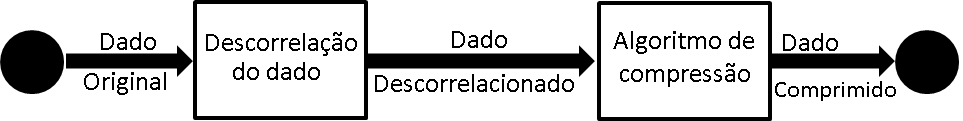
\includegraphics[scale=0.5]{fig/twostagecomp.png}
\caption[Compressão de duas etapas]{Esquema de compressão em duas etapas. Na
primeira, o dado é descorrelacionado para que sua entropia seja diminuida. Na
segunda, um algoritmo de compressão é utilizado.}
\label{Figura:compressaoduasetapas}
\end{figure}

Na segunda etapa, algoritmos clássicos de compressão são utilizados. Como a
solução criada em 1952 por David Albert Huffman e publicada 
em~\citep{Artigo:CodigoHuffman}. A Codificação de Huffman. Uma ideia tão simples
que, segundo~\citep{Book:HuffmanWinZip2}, \textquotedblleft até um aluno do
Ensino Médio poderia entender\textquotedblright. A ideia de Huffman se valia da
probabilidade de cada símbolo único ocorrer no dado de entrada. O algoritmo
baseia-se na criação de uma árvore binária onde cada nó representa um símbolo
do dado. Símbolos com maior número de repetições no dado original
estão mais perto da raiz, enquanto que aqueles com menor probabilidade possuem
maior altura na árvore. Atribuindo-se o bit um aos filhos à esquerda e zero aos
da direita de um nó, obtem-se a nova codificação do símbolo percorrendo a
árvore. 

A Codificação de Huffman é um algoritmo guloso~\citep{Livro:cormen} e é
tida hoje como o primeiro método moderno de compressão existente~\citep{Book:LosslessCompressionHandbook} e utilizado em
programas como Winzip e PKZip~\citep{Book:HuffmanWinZip, Book:HuffmanWinZip2}.
Nos anos que se seguiram, foram feitas diversas tentativas de tornar a
Codificação de Huffman dinâmica, ou seja, capaz de calcular a probabilidade de
cada símbolo aparecer em tempo real, ajustando a árvore construída
dinamicamente sempre que necessário. Destacam-se as soluções propostas
em~\citep{Artigo:KnuthDynamicHuffman} e~\citep{Artigo:VitterDynamicHuffman}.

%Na década de 1960, a Codificação Aritmética, um dos algoritmos mais
%usados nos dias de hoje, utilizado em dezenas, talvez
%centenas de patentes, foi descrita em~\citep{Book:ArithmeticCoding}. A
%Codificação Aritmética também será utilizada nesse trabalho e, por esta razão,
%será explicada mais detalhadamente na seção~\ref{Subsec:CodificacaoAritmetica}.

Outra solução que pode ser usada na segunda etapa é a Codificação
Aritmética~\citep{Book:ArithmeticCoding}.
Como ela será utilizada nesse trabalho, ela será detalhada na
seção~\ref{Subsec:CodificacaoAritmetica}.

\section{A Codificação Aritmética}
\label{Subsec:CodificacaoAritmetica}

A Codificação Aritmética, proposta primeiramente
em~\citep{Book:ArithmeticCoding} e estudada mais a fundo
por~\citep{Artigo:ArithmeticCoding}, faz parte de um dos algoritmos de
compressão mais utilizados atualmente, seja diretamente ou como base para
outras soluções. Diferente dos demais algoritmos, como o de Huffman,
a codificação aritmética não cria um código único para cada símbolo distinto do
dado e depois relê o dado original substituindo cada símbolo pelo seu respectivo
código, ela gera um código que representa todo o dado de
entrada, de forma que trocar dois símbolos de lugar pode criar um código
completamente diferente do anterior. Já na codificação de Huffman, por exemplo,
o código só mudaria nas posições onde houve a troca.

O objetivo do algoritmo é gerar um número entre zero e um a partir do qual o
dado original seja regerado. Como entrada, o algoritmo precisa da probabilidade
de aparecimento de cada símbolo único existente no dado original. O seu
primeiro passo consiste em criar o intervalo $(0, 1]$ e particioná-lo na mesma
quantidade de símbolos distintos do dado original. Cada partição representa um
dos símbolos distintos do dado original, é rotulada de acordo com o símbolo que
representa e possui tamanho proporcional à probabilidade do respectivo símbolo.

No próximo passo, o algoritmo lê o primeiro
símbolo do dado de entrada, encontra a partição a que pertence tal
símbolo e redimensiona o intervalo, que antes era $(0, 1]$, para o tamanho
referente à partição do símbolo lido. Esse processo é repetido para cada
um dos próximos símbolos existentes no dado de entrada, até que eles terminem.

Existe uma técnica capaz de escolher o
melhor número no intervalo calculado na codificação aritmética e facilitar a
decodificação do dado comprimido. Ela se baseia em uma busca binária no
intervalo original, que inicialmente era $(0, 1]$. Nessa condição, o primeiro
número testado seria $0,5$. Se $0,5$ estiver contido no intervalo calculado pela
codificação aritmética, $0,5$ é transformado em binário e enviado ao
decodificador. Se não, testa-se se $0,5$. Se ele for menor do que o limite
inferior do intervalo calculado pela codificação aritmética, o próximo número a ser testado
é $0,75$. Se $0,5$ for maior que o limite superior do intervalo, o próximo
valor a ser testado é $0,25$. Esse processo se repete até que o primeiro número
dentro do intervalo calculado pela codificação aritmética seja encontrado. Este
número é transformado em binário e enviado ao decodificador. %e retornado pela
% função. % O algoritmo~\ref{alg:codifarit} ilustra esse processo.

%O objetivo do~\emph{Arithmetic Encoding} é codificar o dado de entrada gerando
%um número entre zero e um a partir do qual a sequência original possa ser
%recuperada, sem perdas. Diferente de outros métodos de compressão por redução
% de entropia, como o algoritmo de Huffman, que calculam uma sequência distinta
% de bits para cada símbolo, o Arithmetic
%Coding gera uma sequência a partir de todo o dado de entrada.

%Para a compressão, o \emph{Arithmetic Encoding} necessita do dado original e da
%probabilidade de cada símbolo ocorrer para codificar o dado. No início, o
%algoritmo trabalha com um intervalo largo $[0, 1)$ e o vai diminuindo conforme
%novos dados do conjunto a ser codificado são lidos. Símbolos com maior
%probabilidade de aparecimento diminuem o intervalo mais suavemente, enquanto
%os com menor probabilidade achatam o intervalo com mais veemência. O algoritmo
%está abaixo.

%\begin{algorithm}[ht]
%\caption{A Codificação Aritmética}
%\label{alg:codifarit}
%\Entrada {\\ \textbf{\emph{dadoOriginal}} - O dado que se deseja comprimir. \\
%\textbf{\emph{probSimbolos}} - Tabela de dispersão onde uma chave representa um
%símbolo único do dado e o valor dessa chave a probabilidade de tal símbolo
%aparecer.}
%\vspace{1mm}
%\Saida{\\ \textbf{\emph{codificado}} - um número binário a partir do qual o
%dadoOriginal pode ser reconstruído.}
%\vspace{1mm}
%\hrule
%\vspace{1mm}
%\SetKwFunction{rec}{$\leftarrow$}
%\Inicio
%{
%    tamIntervalos \rec probSimbolos.clone()\; 
%    \ParaCada{simboloAtual $\in$ dadoOriginal}
%    {
%    	probAtual \rec probSimbolos [simboloAtual]\;    	%
%		tamIntervalos \rec tamIntervalos $\times$ probAtual\
%    }
%    
%    limite\_inferior \rec min(tamIntervalos.values())\; 
%    limite\_superior \rec max(tamIntervalos.values())\;
%    numero \rec encontra\_melhor\_numero(limite\_inferior, limite\_superior)\; 
%    resposta \rec passa\_para\_binario(numero)\;
%    \Retorna resposta\;
%}
%\end{algorithm}

%A probabilidade de cada símbolo único será exaustivamente consultada no
% decorrer do algoritmo. Por esta razão, optou-se por utilizar uma tabela de dispersão,
%onde os símbolos únicos do dado original são utilizados como chave, e a
%probabilidade do respectivo símbolo o valor associado a ela.

Seja o dado original $A = \{a_1, a_1, a_2, a_1, a_1\}$ e o conjunto de
probabilidades $P = \{P_{a_1} = 0,8; P_{a_2} = 0,2\}$. Deseja-se utilizar a
codificação aritmética para comprimir $A$. Primeiramente, o intervalo $[0, 1)$
é particionado em duas partes, já que existem apenas dois símbolos distintos no
dado original, $a_1$ e $a_2$. Como a probabilidade de $P_{a_1} = 0,8$ e
$P_{a_2} = 0,2$, esse é o tamanho das partições de $a_1$ e $a_2$,
respectivamente. Em seguida, os dados começam a ser lidos. $a_1$ é o primeiro
elemento de A. Como a partição de $a_1$ no intervalo original é delimitada por
$[0,2; 1)$, esses serão os novos limites do intervalo.

A Figura~\ref{fig:arithmeticencoding} ilustra esse processo por iteração. Na
primeira iteração, o intervalo original $(0, 1]$ é calculado, este intervalo é
cortado em $0,2$, formando duas novas partições. Exatamente o mesmo número de
símbolos distintos existentes no dado de entrada. O intervalo é particionado em
$0,2$ justamente porque esta é a probabilidade do símbolo $a_2$ aparecer. O
algoritmo lê o primeiro dado do símbolo original ($a_1$), encontra a partição a
que ele pertence e redimensiona o intervalo para $(0,2, 1]$. Na iteração dois, o
segundo símbolo do dado original é lido ($a_1$) e o intervalo, que antes estava
limitado por $(0,2, 1]$ agora é redimensionado e limitado por $(0,36, 1]$. Na
terceira iteração, o terceiro símbolo do dado original é lido ($a_2$). Agora, a
partição rotulada de $a_1$ é escolhida, e o intervalo original do algoritmo
passa a ser $(0,36, 0,488]$, tamanho da partição de $a_1$ na iteração três. Esse
processo continua até que não existam mais dados a serem lidos.

Uma vez que os símbolos no dado original terminam, tem-se um último intervalo,
delimitado pelo menor e maior tamanhos de partições, respectivamente. Qualquer
número contido nesse intervalo pode ser enviado para o decodificador para que,
junto com as probabilidades de cada símbolo ocorrer, o dado original seja
regenerado, sem perdas.

\begin{figure}[ht]
\centering
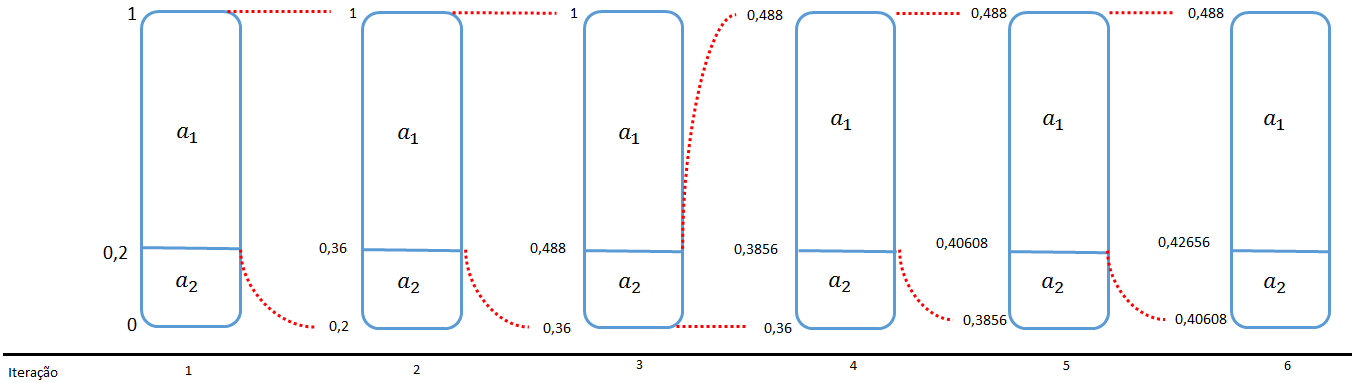
\includegraphics[scale=0.45]{fig/arithmeticencoding.png}
\caption[Ilustração do algoritmo da codificação aritmética]{Ilustração do
algoritmo da codificação aritmética}
\label{fig:arithmeticencoding}
\end{figure}


De acordo com a Figura~\ref{fig:arithmeticencoding}, qualquer número no
intervalo $[0,40608; 0,488)$ pode ser enviado para o decodificador para que haja
a descompressão. Para se escolher o melhor número no intervalo, faz-se uma busca
binária como acima mencionado. O primeiro número testado é $0,5$, pois $(1 + 0)
/ 2 = 0,5$. Como $0,5$ está acima do intervalo superior $0,488$, o próximo valor a
ser testado é $0,25$, pois $(0 + 0,5) / 2 = 0,25$, que está abaixo do intervalo
inferior $0,40608$. A Tabela~\ref{Tabela:codificacaoaritmeticaexemplo} mostra as
iterações do algoritmo de busca binária à procura do primeiro número dentro do
intervalo calculado pela codificação aritmética. O número encontrado foi
$0,4375$.

\begin{table}[ht]
\centering
\begin{tabu}{c|c|c|c}
\tabucline[2pt]{-}
\textbf{Intervalo Inferior} & \textbf{Intervalo Superior} & \textbf{Valor
Testado} & \textbf{Situação} \\
\tabucline[2pt]{-} 0 & 1 & 0,5 & < superior
 \\ 
\hline  
0 & 0,5 & 0,25 & < inferior \\ 
\hline 
0,25 & 0,5 & 0,375 & < inferior \\ 
\hline 
0,375 & 0,5 & 0,4375 & Dentro do intervalo \\ 
\tabucline[2pt]{-}
\end{tabu} 
\caption[Iteração algoritmo codificação aritmética]{Exemplo iteração algoritmo
codificação aritmética}
\label{Tabela:codificacaoaritmeticaexemplo}
\end{table}

Para a descompressão, o valor $0,4375$ bem como a probabilidade de cada símbolo
único ocorrer são suficientes. Algumas implementações também pedem a quantidade
de símbolos existentes no dado original para facilitar o processo. A grande
vantagem da codificação aritmética é que ela tende para a entropia do dado. Em
outras palavras, seja um dado hipotético de tamanho infinito, é possível provar
que a entropia do dado gerado pela codificação aritmética tende a $H$
(equação~\ref{eq:entropia})~\citep{Artigo:ArithmeticCoding}. Como desvantagens,
a codificação aritmética sofre do risco de truncamento, caso o número calculado
pelo algoritmo contenha muitas casas decimais. Ademais, a codificação aritmética
foi projetada para funcionar com números inteiros e em intervalos contínuos.
 
 %Em linhas gerais, o algoritmo inicia com um intervalo entre zero e um,
 %particiona-o em $k$ pedaços, sendo $k$ o número de símbolos únicos no dado
 %original. Cada pedaço tem o tamanho proporcional à probabilidade do símbolo
 %aparecer e receberá um rótulo para identificar o símbolo a que ele pertence.
 
 %A partir de então, o algoritmo lê cada símbolo do dado original, encontra a
 %partição referente àquele símbolo e assume o intervalo atual como o da
 %% partição do símbolo encontrado. Dessa forma, o intervalo que antes variava
 % entre $[0,
 %1)$, agora varia de acordo com o intervalo $[SP_{s - 1}, SP_{s - 1} +
 % SP_{s})$, onde $SP_{s-1}$ representa a soma dos tamanhos das partições
 % anteriores à do
 %símbolo atual e $SP_s$ o tamanho da partição atual. Essa operação é repetida
 % enquanto houver símbolos no dado original a serem lidos.
		
%A grande vantagem do \emph{Arithmetic Encoding} é que ele chega perto da
% entropia do dado, sem que haja um pré-requisito nele (por exemplo, a
% codificação de Huffman só alcança a entropia máxima se a probabilidade dos
% símbolos ocorrerem forem potências de dois). A desvantagem do  \emph{Arithmetic
% Encoding} é que, quanto mais símbolos distintos o dado original possui, mais
% ineficiente a compressão se torna, pois símbolos que pouco aparecem diminuem o
% intervalo bruscamente, aumentando a quantidade de casas decimais a serem
%enviadas para o decodificador. 

%O \emph{Arithmetic Encoding} é adequado quando se percebe que o número de
%ocorrências de um símbolo no dado é muito maior que a soma das ocorrências dos
%demais. Uma vantagem do algoritmo é que, nessas condições, ele chega
%perto da entropia do dado. Uma desvantagem é que o algoritmo não funciona bem
%com um número grande de símbolos.

%\subsection{O algoritmo de Stearns}

%Para contornar os problemas descritos anteriormente, Stearns propôs
%em~\citep{Artigo:stearn} um método para limitar a quantidade de símbolos do
%dado original. A ideia é fazer com que o Arithmetic Coding visualize vários
% símbolos como um só. Para isso, criam-se os vetores chamados~\emph{bin}
% e~\emph{offset}.
%Além disso, mais um parâmetro é escolhido, o~\emph{nbin}, que significa quantos
%símbolos o Arithmetic Coding deve enxergar.

\subsection{O algoritmo de Stearns}
\label{Paragrafo:stearns}

Para contornar os problemas acima citados, Stearns
propôs um método para limitar a quantidade de símbolos do dado original e
transformá-los em inteiros~\citep{Artigo:stearn}. O algoritmo de Stearns deve
ser rodado antes do dado ser enviado à codificação aritmética. Seja $A$ o dado
que se deseja comprimir utilizando codificação aritmética, Stearns propõe que
todos os elementos de $A$ sejam divididos por um mesmo valor. Essa divisão deve
ser inteira. Posteriormente, o resto das divisões por esse mesmo valor 
deve ser calculado. Dessa forma, de $A$ foram obtidas duas novas séries
numéricas $A_B$, com os quocientes das divisões e $A_O$ com os restos. Ambas
inteiras.
 
Idealmente, espera-se utilizar um divisor que crie muitos valores repetidos em
$A_B$, de forma que a contagem de elementos em $A_B$ siga uma distribuição
gaussiana. A contagem de elementos de $A_O$, em contrapartida, deve gerar uma
distribuição uniforme. $A_B$ é, então, comprimido com codificação aritmética e
$A_O$ não sofre qualquer compressão. 

O Algoritmo~\ref{Algoritmo:Stearns} descreve a criação de Stearns. As linhas 2
e 3 nada mais fazem do que iniciar os vetores $A_O$ e $A_B$. A
função~\emph{zeros} retorna um vetor de $|A|$ elementos, todos iguais a zero.
Na linha 4, o contador $i$ é iniciado. A linha 5 estabelece a condição de parada do algoritmo,
já que $|A|$ designa o número de elementos de A.

A linha 6 indica que o resto da divisão do elemento na posição $i$ do vetor A
por nbin será guardado na posição $i$ do vetor $A_O$. Na linha 7, o quociente,
arredondado para baixo, da divisão do elemento na posição $i$ do vetor A por
nbin é guardado na posição $i$ do vetor $A_B$. A linha 8 incrementa o índice
atual dos vetores e a linha 10 retorna o resultado obtido.

\begin{algorithm}[ht]
\caption{Algoritmo desenvolvido no trabalho de~\citep{Artigo:stearn} para
diminuir o número de símbolos para compressão com a codificação aritmética}
\label{Algoritmo:Stearns}
\Entrada 
{
\begin{description}
  \item[A]\\
  	Vetor contendo o conjunto de números sobre os quais deseja-se aplicar o
  	algoritmo de Stearns
  \item[nbin]\\
  	Número inteiro indicando o número máximo de símbolos distintos que \textbf{A}
  	deve conter
\end{description}
}
\vspace{1mm}
\Saida
{
\begin{description}
  \item[$A_O$]\\
  	Vetor de restos das divisões.
  \item[$A_B$]\\
  	Vetor com o quociente das divisões.
\end{description}
}
\vspace{1mm}
\hrule
\vspace{1mm}
\SetKwFunction{rec}{$\leftarrow$}
\Inicio
{
	$A_O$ \rec zeros($|A|$)\;
	$A_B$ \rec zeros($|A|$)\;
	i \rec 0\;
	\Enqto{i $< |A|$ }
	{
		$A_O$[i] \rec resto\_divisao(A[i], nbin)\;
		$A_B$[i] \rec $\displaystyle \floor[\Bigg]{\frac{A[i]}{nbin}}$\;
		i++\;
	}
	\Retorna $\{A_O, A_B\}$\;
}
\end{algorithm}

Suponha o vetor $A = \{52, 54, 55, 50, 53, 58, 47, 51, 56, 59\}$ e o valor de
nbin igual a 10. A aplicação do algoritmo de Stearns resultaria nos vetores
$A_B = \{5, 5, 5, 5, 5, 5, 4, 5, 5, 5\}$ e $A_O = \{2, 4, 5, 0, 3, 8, 7, 1, 6,
9\}$. $A_B$ é então comprimido pela codificação aritmética e $A_O$ é enviado
para o decodificador sem nenhum tipo de compressão.

\begin{figure}[ht]
\centering
\begin{subfigure}{.49\textwidth}
  \centering
  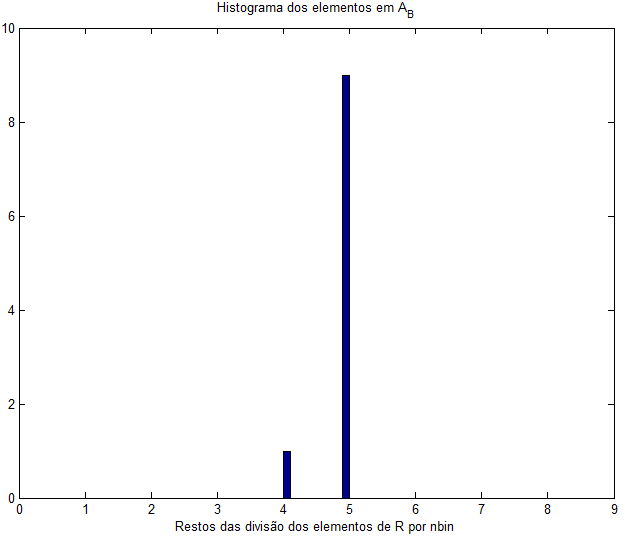
\includegraphics[width=1\linewidth]{fig/histxb.png}  
  \caption{Histograma dos quocientes das divisões dos elementos de A por nbin.}
  \label{fig:histab}
\end{subfigure}%
\hfill
\begin{subfigure}{.49\textwidth}
  \centering
  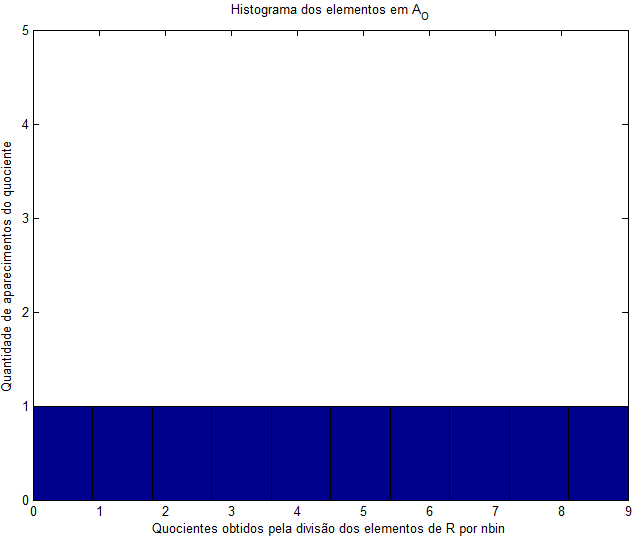
\includegraphics[width=1\linewidth]{fig/histxo.png}
  \caption{Histograma dos restos das divisões dos elementos de A por nbin.}
  \label{fig:histao}
\end{subfigure}
\caption[Histogramas gerados pela aplicação do algoritmo de Stearns]{À esquerda
o histograma segue uma distribuição gaussiana.
À direita o histograma segue uma uma distribuição uniforme. Esse é o resultado ideal da
aplicação do algoritmo de Stearns.}
\label{fig:naoestacionariaeestacionaria}
\end{figure}
         % Editar o arquivo introducao.tex
\chapter{Análise de séries temporais}
\label{Capitulo:analisedeseriestemporais}

O objetivo deste capítulo é a introdução de alguns conceitos relativos a séries
temporais e modelos utilizados para modelá-las e prever seus próximos valores.

\section{Conceitos iniciais}

Existem, na literatura, diversas definições para o termo \emph{série temporal}.
A definição proposta em~\citep{Livro:analiseseriestemporais} parece ser mais
abrangente. Nela, o autor caracteriza uma série temporal como uma realização de
um processo estocástico. Já~\citep{Livro:estatisticaadmeeconomia} a conceitua
como dados observados em~\emph{n} períodos, restringindo sua definição a séries
temporais discretas. O mesmo faz~\citep{Livro:serietemporal2}, onde as séries
temporais são formalmente definidas como um conjunto de variáveis aleatórias
indexadas no tempo. Neste trabalho as séries temporais sempre serão discretas.
Portanto, as três definições acima são aceitáveis.

Uma série temporal pode ser caracterizada, ainda, como estacionária ou não
estacionária. Uma série estacionária é aquela que flutua ao redor de uma média
ao longo do tempo. A Figura~\ref{fig:exestacionaria} apresenta o exemplo de uma
série estacionária, enquanto na Figura~\ref{fig:exnaoestacionaria} é exibido um
exemplo de uma série não estacionária. A fim de se tornar uma série não
estacionária em estacionária, calcula-se a diferença entre seus termos
consecutivos. Seja $Z$ uma série temporal e $\Delta^d$ o operador diferença,
sendo $d$ a quantidade de diferenças a ser calculada, a
Equação~\ref{eq:diferenca} mostra a criação de uma nova série, $W$, formada pela
$d$-ésima diferença da série $Z$.

\begin{figure}[ht]
\centering
\begin{subfigure}{.49\textwidth}
  \centering
  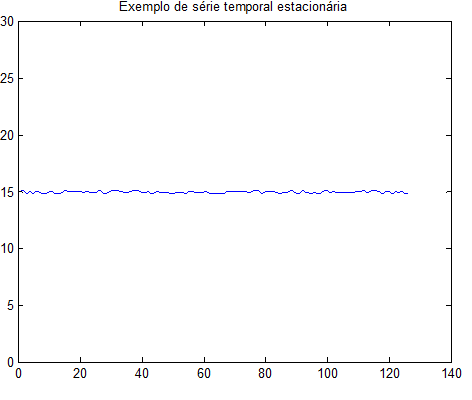
\includegraphics[width=1\linewidth]{fig/serieestacionaria.png}  
  \caption{Exemplo de série estacionária.}
  \label{fig:exestacionaria}
\end{subfigure}%
\hfill
\begin{subfigure}{.49\textwidth}
  \centering
  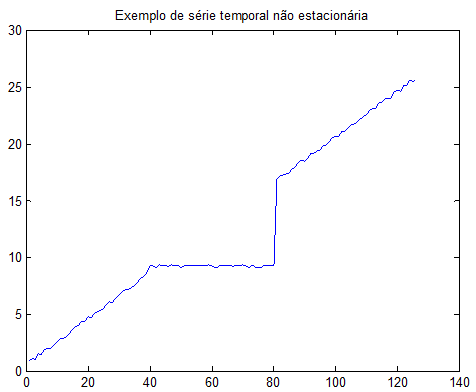
\includegraphics[width=1\linewidth]{fig/serienaoestacionaria.png}
  \caption{Exemplo de série não estacionária.}
  \label{fig:exnaoestacionaria}
\end{subfigure}
\caption{À esquerda o exemplo de uma série estacionária. À direita o exemplo de
uma série não estacionária.}
\label{fig:naoestacionariaeestacionaria}
\end{figure}

\begin{equation}
W = \Delta^dZ
\label{eq:diferenca}
\end{equation}

\begin{figure}[ht]
\centering
\begin{subfigure}{.49\textwidth}
  \centering
  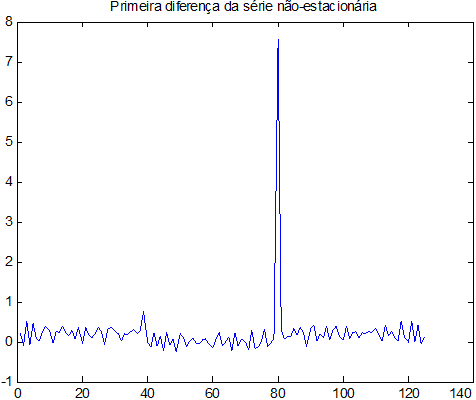
\includegraphics[width=1\linewidth]{fig/serieprimeiradiferenca.png}  
  \caption{Resultado da aplicação da equação~\ref{eq:diferenca} com $d=1$ na
  figura~\ref{fig:exnaoestacionaria}.}
  \label{fig:d1}
\end{subfigure}%
\hfill
\begin{subfigure}{.49\textwidth}
  \centering
  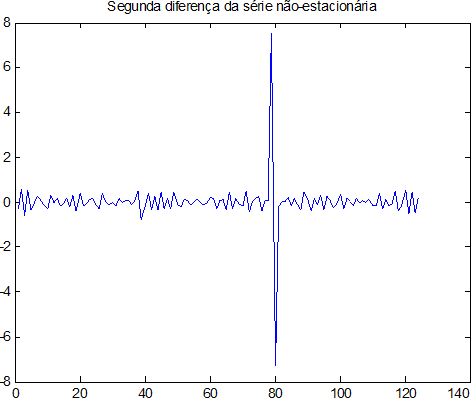
\includegraphics[width=1\linewidth]{fig/seriesegundadiferenca.png}
  \caption{Resultado da aplicação da equação~\ref{eq:diferenca} com $d=2$ na
  figura~\ref{fig:exnaoestacionaria}.}
  \label{fig:d2}
\end{subfigure}
  \caption{Tornando a figura~\ref{fig:exnaoestacionaria} em
  estacionária através da equação~\ref{eq:diferenca}.}
\label{fig:d1ed2}
\end{figure}

Aplicando-se a Equação~\ref{eq:diferenca} sobre a série da
Figura~\ref{fig:naoestacionariaeestacionaria}, obtem-se os resultados expostos
na Figura~\ref{fig:d1ed2}. É possível ver que, para $d=1$, a série ainda não se
tornou estacionária, necessitando de mais uma diferença para fazê-lo. Em geral, duas diferenças são suficientes para tornar
a série estacionária~\citep{Livro:analiseseriestemporais}.

Uma série temporal é dita~\emph{homocedástica} se sua variância puder ser
considerada constante ao longo do tempo. Caso contrário, a série é chamada
de~\emph{heteroscedástica}. A Figura~\ref{Figura:exemplodedadohomocedastico}
apresenta uma série temporal homocedástica ao passo que as
Figuras~\ref{Figura:exemplodedadoheterocedasticosismico}
e~\ref{Figura:exemplodedadoheterocedasticoaudio} apresentam exemplos de dados
heteroscedásticos.

\begin{figure}[!ht]
\centering
\begin{subfigure}{.49\textwidth}
  \centering
  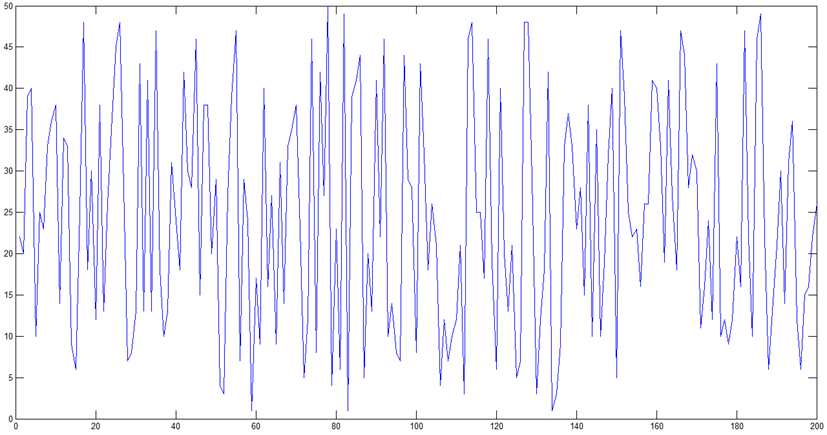
\includegraphics[width=1\linewidth]{fig/homocedastico.png}  
  \caption{Exemplo de dado homocedástico}
  \label{Figura:exemplodedadohomocedastico}
\end{subfigure}%
\hfill
\begin{subfigure}{.49\textwidth}
  \centering
  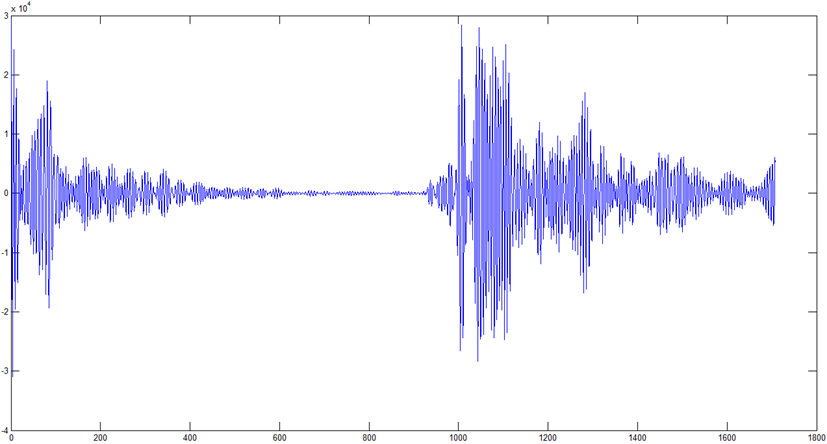
\includegraphics[width=1\linewidth]{fig/tracosismico.png}
  \caption[Exemplo de dado heteroscedástico]{O traço sísmico é um exemplo de
  dado heteroscedástico}
  \label{Figura:exemplodedadoheterocedasticosismico}
\end{subfigure}\\[1ex]
\begin{subfigure}{.49\textwidth}
  \centering
  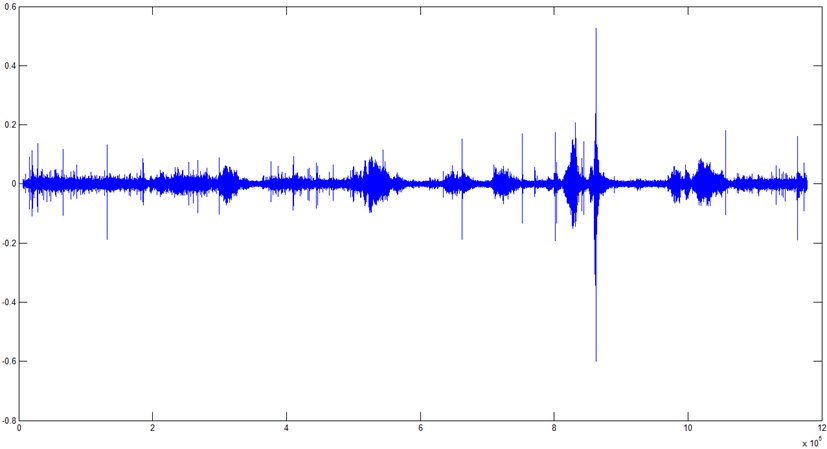
\includegraphics[width=1\linewidth]{fig/tracoaudio.png}
  \caption{O dado de áudio gerado por voz humana e captado por um microfone
  também é exemplo de dado heteroscedástico.}
  \label{Figura:exemplodedadoheterocedasticoaudio}
\end{subfigure}
  \caption{Exemplos de dados homo e heterocedásticos.}
\label{Figura:exemplosdadoshomoehetero}
\end{figure} 

Nas próximas seções são apresentados alguns modelos estatísticos que serão úteis
nesse trabalho.

\section{Modelo Autoregressivo}

Seja $Z$ uma série temporal de $x$ elementos $Z = \{Z_0, Z_1, \hdots, Z_{x-1}\}$
e $t$ um momento no tempo válido para $Z$, ou seja, $0 \leq t < x$. Sendo assim,
$Z_t$ é um valor de $Z$ no momento $t$. Agora, consideremos o problema de se obter o valor
$Z_t$ dado os $p$ valores anteriores imediatamente consecutivos. Para início,
considerando $p = 1$, $Z_t$ depende apenas do valor de $Z_{t-1}$, $Z_{t-1}$ de
$Z_{t-2}$ e assim por diante. Não parece razoável estabelecer a simples relação
$Z_{t} = Z_{t-1}$, pois em nenhum momento foi dito que $Z_t$ realiza uma série
temporal constante.

A relação $Z_t = \alpha_1Z_{t-1}$ aparece como uma alternativa mais
interessante nesse cenário. Entretanto, diz-se impossível encontrar um único
valor de $\alpha_1$ que satisfaça todas as possíveis igualdades, a saber:
$Z_2 = \alpha_1Z_{t1}$, $Z_3 = \alpha_1Z_{t2}$, $Z_4 = \alpha_1Z_{t3}$,
$\hdots$, $Z_t = \alpha_1Z_{t-1}$. Para resolver esse problema, utiliza-se
a relação presente na equação $Z_t = \alpha_1Z_{t-1} +
\epsilon_t$, em que um termo de erro ($\epsilon_t$) é adicionado. Para
contemplar séries em que a média, aqui representada pelo termo $\alpha_0$, não é
zero, a Equação~\ref{eq:ar1} é utilizada.

\begin{equation}
Z_t = \alpha_0 + \alpha_1Z_{t-1} + \epsilon_t
\label{eq:ar1} 
\end{equation}

Considerando agora $p=2$, obtém-se o valor de $Z_t$ através da relação $Z_t =
\alpha_0 + \alpha_1Z_{t-1} + \alpha_2Z_{t-2} + \epsilon_t$. Para $p=3$, vale a
relação $Z_t = \alpha_0 + \alpha_1Z_{t-1} + \alpha_2Z_{t-2} + \alpha_3Z_{t-3} +
\epsilon_t$. De uma forma geral, tem-se:

\begin{equation}
\displaystyle Z_t = \alpha_0 + \sum_{i=1}^p \alpha_iZ_{t-i} + \epsilon_t
\label{eq:ar} 
\end{equation}
 
A Equação~\ref{eq:ar} representa o modelo autoregressivo de ordem $p$, uma
generalização do modelo representado na Equação~\ref{eq:ar1}, em que $p=1$.
Portanto, um modelo autoregressivo é pura e simplemente uma regressão linear de
ordem $p$.

Como dito anteriormente, encontrar um conjunto de parâmetros $\alpha$ que
satisfaça a todas as desigualdades existentes é dito impossível em muitos casos.
O desafio é encontrar um conjunto de parâmetros que miniminize o conjunto de
erros $\{\epsilon_0, \epsilon_1, \hdots, \epsilon_{x-1}\}$. Diz-se que um modelo
é ``bem calculado'' \label{Paragrafo:bemcalculado} se encontra um conjunto de
alfa que minimiza o conjunto de erros. Além disso, um modelo
bem calculado também gera um conjunto de erros descorrelacionados~\citep{Livro:analiseseriestemporais}.

\section{Modelo de Médias Móveis}

A fórmula do modelo de médias móveis (Equação~\ref{eq:mediasmoveis}) é muito
parecida com a o do modelo autoregressivo. Entretanto, o modelo de médias
móveis é conceitualmente uma regressão linear da diferença dos termos anteriores da série
com choques aleatórios e termos de erros originados de algum tipo de ruído
(como ruído branco, por exemplo)~\citep{Livro:analiseseriestemporais}. Mais
claramente, enquanto que o modelo autoregressivo utiliza os $t-p$ termos
anteriores para tentar calcular o atual, o modelo de média móveis utiliza os
$t-q$ erros anteriores para tentar encontrar o termo atual, sendo $q$ a ordem
do modelo de médias móveis.
%Para se utilizar o modelo de médias móveis, deve-se primeiro utilizar um modelo preditor,
% calcular o termo de erro para, finalmente, utilizá-lo no modelo de médias móveis.

\begin{equation}
Z_t = \theta_0 + \sum_{i=1}^q \theta_i\epsilon_{t-i} + \epsilon_t
\label{eq:mediasmoveis}
\end{equation}

Na equação~\ref{eq:mediasmoveis}, $\theta_0$ é a média da série,
$\theta_{t-1,t-2,\hdots,t-q}$ são os coeficientes do modelo e 
$\epsilon_{1,2,\hdots,t}$ representa a diferença entre o valor real da
série e o calculado pelo preditor. Esse erro é também chamado de~\emph{resíduo}.


O papel do choque aleatório em um modelo de médias móveis é diferente do modelo
autoregressivo de duas formas. Primeiro, porque eles são propagados a valores
futuros do modelo de forma direta, já que o termo $\epsilon_{t-1}$ aparece na
parte direita da equação de $Z_t$. No modelo autoregressivo, essa propagação
ocorre de forma indireta, pois $\epsilon_{t-1}$ aparece na fórmula de $Z_{t-1}$
mas não na de $Z_t$, embora $Z_{t-1}$ esteja na fórmula de $Z_t$. Segundo,
porque um choque no modelo de médias móveis afeta $Z$ durante os
próximos $q$ períodos apenas, enquanto que no modelo autoregressivo um choque afeta o modelo até o
final, embora a influência desse choque tenda a zero conforme $t$
aumenta~\citep{Livro:analiseseriestemporais}.

\section{Modelo Autoregressivo de médias móveis}

O modelo autoregressivo de médias móveis, comumente conhecido como modelo
ARMA($p$, $q$), em que $p$ e $q$ são os parâmetros autoregressivo e de médias
móveis, foi originalmente descrito no ano de 1951 na
tese de Peter Whistle~\citep{Livro:whitle1951hypothesis} e popularizado no livro
de George Edward Pelham Box e Gwilym Jenkins~\citep{Livro:box1976times}.


O modelo ARMA(1, 1) é definido como $Z_t = c + \alpha_{1} Z_{t-1} +
\theta_{1}\epsilon_{t-1} + \epsilon_t$, em que $c$ é a média da série,
$\alpha_{1, 2, \hdots, p}$ e $\theta_{1, 2, \hdots, q}$ são os coeficientes
do modelo autoregressivo e de médias móveis, respectivamente. A
Equação~\ref{eq:arma} apresenta o modelo ARMA($p$, $q$).

\[
Z_t = c + \alpha_1Z_{t-1} + \alpha_2Z_{t-2} + \hdots + \alpha_pZ_{t-p} +
\theta_1\epsilon_{t-1} + \theta_2\epsilon_{t-2} + \hdots +
\theta_q\epsilon_{t-q} + \epsilon_t
\]

\begin{equation}
Z_t = c + \sum_{i=1}^p \alpha_iZ_{t-i} + \sum_{i=1}^q \theta_i\epsilon_{t-i} +
\epsilon_t
\label{eq:arma}
\end{equation}

%O grande desafio nesse modelo é encontrar os valores de $\alpha_{1, 2, \hdots,
%p}$ e $\theta_{1, 2, \hdots, q}$ que miniminize os erros $\epsilon_{1, 2,
%\hdots, t}$.

%Eventualmente, utiliza-se do operador de defasagem $L$
%(equação~\ref{eq:lagoperator}) para reescrever a equação~\ref{eq:arma} da forma
%exposta na equação~\ref{eq:armadef}. As duas equações expressam exatamente a
% mesma coisa.

%A equação~\ref{eq:arma} é comumente reescrita como na equação~\ref{eq:armadef}
%na literatura.

%\begin{equation}
%\displaystyle \left(1 - \sum_{i=1}^p \alpha_iL^i\right)Z_t =
%\left(1+\sum_{i=1}^q\theta_iL^i\right)\epsilon_t\text{,}
%\label{eq:armadef}
%\end{equation}

%\noindent onde $L$ é o operador de defasagem especificado em um valor $k$, onde
%$-t < k < t$.

%\begin{equation}
%\displaystyle L^kZ = Z_{t-k} 
%\label{eq:lagoperator}
%\end{equation}

%Como dito acima, $k$ também aceita valores negativos. Dessa forma, se $k=-1$,
%obtém-se a igualdade abaixo.

%\[
%L^{-1}Z_t = Z_{t+1}
%\]

O modelo ARMA($p$, $q$) mostrou-se uma opção poderosa e vem vendo usado até os
dias de hoje. O seu único problema, entretanto, é que ele funciona apenas com
séries estacionárias. Para contornar essa limitação, projetou-se um novo modelo
a partir do modelo ARMA, o ARIMA.

\section{Modelo Autoregressivo integrado de médias móveis}

O modelo ARIMA($p$, $d$, $q$) é uma generalização do modelo ARMA($p$, $q$)
porque também funciona com séries não-estacionárias. Os parâmetros $p$ e $q$
continuam representando, respectivamente, a ordem dos modelos autoregressivo e
de médias móveis, enquanto $d$ refere-se à quantidade de diferenças aplicadas à
série para torná-la estacionária. Utilizando a Equação~\ref{eq:diferenca}, o
modelo ARIMA($p$, $d$, $q$) pode ser especificado conforme a
Equação~\ref{eq:arima}.

\begin{equation}
W_t = c + \alpha_1W_{t-1} + \alpha_2W_{t-2} + \hdots + \alpha_pW_{t-p} +
\theta_1\epsilon_{t-1} + \theta_2\epsilon_{t-2} + \hdots +
\theta_q\epsilon_{t-q} + \epsilon_t
\label{eq:arima}
\end{equation}

O modelo existente na equação~\ref{eq:arima} sugere que os valores de
$W_{1,2,\hdots}$ no momento $t$ podem ser previstos baseados nos $p$ valores
antecessores e nos $q$ resíduos antecessores da série original $Z$. De uma forma
geral, a sequência dos erros, $\epsilon$, é considerada um ruído branco
gaussiano, variáveis aleatórias seriamente descorrelacionadas que possuem
distribuição Gaussiana, com média zero e variância finita.

A Equação~\ref{eq:arima} pode ser reescrita da seguinte forma:

\[
W_t - \alpha_1W_{t-1} - \alpha_2W_{t-2} - \hdots - \alpha_{t-p}W_{t-p} = c +
\theta_1\epsilon_{t-1} +\theta_2\epsilon_{t-2} + \hdots + \theta_q\epsilon_{t-q}
+ \epsilon_t
\]

Considerando $\overline{AR}_p$ como o operador autoregressivo que especifica
uma auto-regressão dos últimos $p$ valores da série e o operador de médias
móveis $\overline{MA}_q$ que especifica médias móveis de ordem $q$, a
equação acima pode ser reescrita da seguinte forma:

\[
\displaystyle \overline{AR}_p(W_t) = \overline{MA}_q\left(\epsilon_t\right)
\Leftrightarrow \overline{AR}_p\left(\Delta^d Z_t\right) =
\overline{MA}_q\left(\epsilon_t\right)
\]

Nota-se que os termos de $\Delta^dZ_{t=1,\hdots,p}$ são as diferenças entre os
termos de $Z_{t=1,2,\hdots,p+d}$ e, por isso, o modelo pode ser representado da
seguinte forma:

\[
\overline{AR}_{p+d}\left(Z_t\right) = \overline{MA}_q\left(\epsilon_t\right)
\]

Os termos de $Z$ podem ser obtidos através da seguinte relação:

\[
Z_t = c + \phi_1Z_{t-1}+\phi_2Z_{t-2}+\hdots+\phi_{p+d}Z_{t-(p+d)} +
\theta_1\epsilon_{t-1} + \theta_2\epsilon_{t-2} + \hdots +
\theta_q\epsilon_{t-q}
\]

Ou seja, para predizer valores através do modelo ARIMA($p$, $d$, $q$), são
necessários os parâmetros $\phi_{1,2,\hdots,p+d}$, as últimas $p+d$ amostras da
série $Z_{t-(p+d), \hdots, i-2, i-1}$, os $q$ parâmetros $\theta_{1,2,\hdots,q}$
e os últimos $q$ resíduos $\epsilon_{t-1, t-2, \hdots, t-q}$.

\section{Modelo Autoregressivo com heteroscedasticidade condicional
generalizado}

O modelo Autoregressivo com heteroscedasticidade condicional
generalizado (GARCH)~\citep{Artigo:garch} é uma extensão do modelo
Autoregressivo com heteroscedasticidade condicional
(ARCH)~\citep{Artigo:arch}. Seu objetivo é trabalhar com séries temporais que
sejam heteroscedásticas, estimando um valor mais real para o resíduo
$\epsilon_i$, onde $0<i\leq t$.

O modelo GARCH é capaz de prever a variância de uma série temporal utilizando os
seus últimos valores. O modelo possui dois componentes $(\overline{p},
\overline{q})$. $\overline{p}$ corresponde ao número de termos GARCH a serem
utilizados, enquanto $\overline{q}$ corresponde ao número de termos
ARCH~\citep{Artigo:joe}.

O modelo GARCH $(\overline{p}, \overline{q})$ aplicado sobre a série
temporal $\delta$, possui o formato da Equação~\ref{eq:garch}, onde
$\overline{\alpha}_{0,1,\hdots,\overline{p}}$,
$\overline{\beta}_{0,1,\hdots,\overline{q}}$ e $\overline{\gamma}$ são
parâmetros do modelo, $\eta_t$ é, em geral, um processo Gaussiano com média zero
e variância constante.

\[
\delta_t = \eta_t\sqrt{h_t} \text{,}
\]
\vspace{1cm}
\begin{equation}
h_{t+1} = \overline{\alpha}_0\delta_t^2 + \overline{\alpha}_1\delta_{t-1}^2 +
\hdots + \overline{\alpha}_{\overline{p}-1}\delta_{t-(\overline{p}-1)}^2 +
\overline{\beta}_0h_t + \overline{\beta}_1h_{t-1} + \hdots +
\overline{\beta}_{\overline{q}}h_{t-(\overline{q}-1)} + \overline{\gamma}
\label{eq:garch}
\end{equation}

\section{Modelo ARIMA junto com modelo GARCH}

É possível combinar os modelos ARIMA e GARCH e gerar um novo modelo,
ARIMA-GARCH, ou seja, um modelo ARIMA com a variância do GARCH. Em um modelo
ARIMA($p$, $d$, $q$)-GARCH($\overline{p}$, $\overline{q}$) os resíduos
$\epsilon_{1,2,\hdots,t}$ são modelados através do modelo GARCH, da seguinte
forma:

\[
Z_t = \epsilon_t + \phi_1Z_{t-1} + \phi_2Z_{t-2} + \hdots + \phi_{p+d}Z_{t-p+d}
+ \theta_1\epsilon_{t-1} + \theta_2\epsilon_{t-2} + \hdots +
\theta_q\epsilon_{t-q}\text{,}
\]
\[
\epsilon_t = \eta_t\sqrt{h_t}\text{,}
\]
\vspace{1cm}
\begin{equation}
h_{t+1} = \overline{\alpha}_0\epsilon_t^2 + \overline{\alpha}_1\epsilon_{t-1}^2
+ \hdots + \overline{\alpha}_{\overline{p}-1}\epsilon_{t-\overline{p}-1}^2 +
\overline{\beta}_0h_t + \overline{\beta}_1h_{t-1} +
\overline{\beta}_{\overline{q}}h_{i - \overline{q} - 1} + \overline{\gamma}
\label{eq:arimagarch}
\end{equation}

Esse modelo possui os parâmetros $\phi_{1, 2, \hdots, p+d}$, $\theta_{1, 2,
\hdots, q}$, $\overline{\alpha}_{0, 1, \hdots, \overline{p}}$,
$\overline{\beta}_{0, 1, \hdots, \overline{q}}$ e $\overline{\gamma}$. A tarefa
agora é resolver um problema de otimização para estimar os melhores valores
desses parâmetros para gerar a menor variância possível dos resíduos. A
resolução desse problema foi feita através da Programação Quadrática
Sequencial.

A Programação Quadrática Sequencial (PQS) é um dos mais bem sucedidos métodos
para a solução numérica de problemas de otimização
não-linear~\citep{NaoPublicado:OptimizationI}. Seja um problema que consiste na
minimização de uma função sujeita a um conjunto de restrições, uma sequência de
subproblemas é construída. A função objetivo é substituída por uma aproximação
quadrática e as restrições são substituídas por aproximações lineares. Daí o
nome de Programação Quadrática Sequencial~\citep{RelatorioTecnico:ProgQuad}.

Mais especificadamente, a PQS se baseia em um procedimento iterativo que modela
o problema para uma dada iteração $x^k$, $k \in \mathbb{N}_+^*$, através da
utilização de soluções envolvendo programação quadrática. O método usa a
iteração atual para construir uma nova iteração $x^{k+1}$. Essa construção é
feita de tal forma que a solução convirja para um mínimo local quando $k
\rightarrow \infty$. A presença de restrições na PQS faz com que tanto a
análise quanto a implementação dela sejam bem complicadas.

A explicação a fundo da PQS é bem complexa e foge do escopo desse trabalho.
Para mais informações, recomenda-se o capítulo
18 do material~\citep{LIVRO:Optimization}.

Uma vez calculados os valores dos parâmetros ARIMA ($\phi_{1, 2, \hdots, p+d}$,
$\theta_{1, 2, \hdots, q}$) e as últimas $d+p$ amostras da série temporal $Z$, é
possível predizer os valores dos próximos elementos de $Z$. Levando-se em
consideração o modelo de variância do GARCH, a série de resíduos tende a ter uma
variância baixa.

\chapter{Método de compressão proposto}
\label{Capitulo:propostatrabalho}

Um modelo matemático linear capaz de modelar uma série temporal a fim de
prever seus próximos termos é chamado de~\emph{modelo de predição linear}. Os
modelos AR e ARMA são modelos de predição linear. Em
diversos trabalhos de compressão de dados, os autores não entram no mérito do
modelo que foi utilizado, apenas se limitam a dizer que foi utilizada uma
predição linear. Nos trabalhos relacionados abaixo, em razão do poder
computacional existente na época em que foram propostos, e por descreverem que
apenas um conjunto de pesos foi criado pelo modelo, aceita-se que o
termo~\emph{predição linear} refira-se ao modelo autoregressivo.

Como já explicado, dados sísmicos são heteroscedásticos. Com o levantamento
bibliográfico descrito na Seção~\ref{Sec:trabalhosrelacionados}, descobrimentos
que o modelo de previsão linear já foi largamente explorado na compressão sem
perdas de dados sísmico. Porém, não fomos capazes de encontrar trabalhos que
lidem diretamente com sua característica heteroscedástica. Este trabalho se
propõe a estudar como a heteroscedasticidade pode ser explorada na primeira fase
de compressão de dados sísmicos, a fim de se obter um conjunto de resíduos
decorrelacionado e com menor entropia. 

Embora a heteroscedasticidade possa ser modelada através de redes neurais
artificiais~\citep{Artigo:rnheteros}, esse trabalho se propõe a utilizar os
modelos ARIMA-GARCH na primeira fase de compressão. Para completar o ciclo de
compressão, o algoritmo de Stearns, explicado na
Seção~\ref{Paragrafo:stearns}, junto com a codificação aritmética, serão
utilizados. A Figura~\ref{fig:tracoeresiduo} ilustra o desejado. Em azul, o
traço sísmico original. Em verde, um exemplo de resíduo esperado pela aplicação
do modelo ARIMA-GARCH, com variância bem menor.

\begin{figure}[ht]
\centering
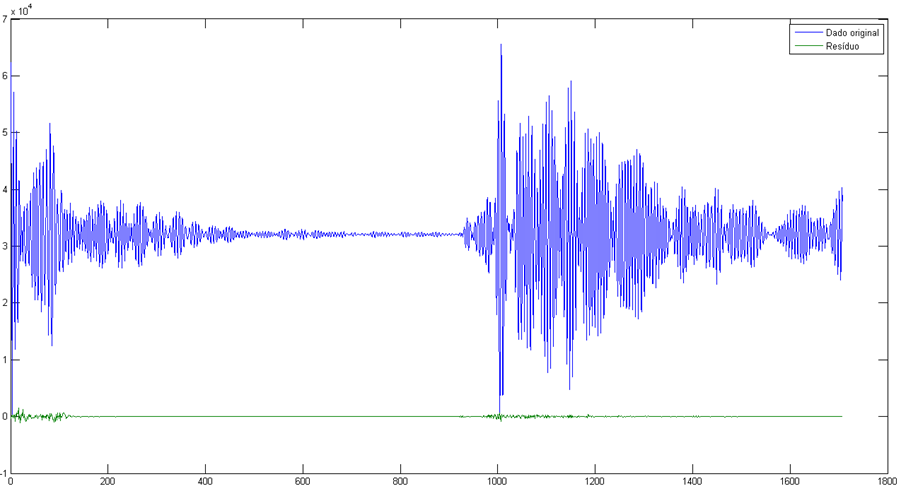
\includegraphics[scale=0.65]{fig/tracoeresiduo.png}
\caption{A linha azul representa um traço sísmico. A linha verde representa o
resíduo calculado a partir desse traço sísmico.}
\label{fig:tracoeresiduo}
\end{figure}

\section{Revisão de trabalhos relacionados}
\label{Sec:trabalhosrelacionados}

Definitivamente, a utilização de predição linear não é novidade na compressão de
dados sísmicos. Movido pela sua ampla utilização, na época, em
processamento de voz,~\citep{Artigo:bordley1983} utilizou a predição linear para a compressão de
dados sísmicos, porém com perdas. Mais tarde, com o
mesmo objetivo,~\citep{Artigo:linearmelhor} mostrou que a predição linear
obteve resultados melhores que as Transformada Discreta de Fourier, Transformada Discreta do Cosseno, Transformada de Walsh-Hadamard e a Tranformada
de Karhunen-Loeve. No trabalho de~\citep{Artigo:stearnsincompleto} são
apresentados, pela primeira vez, o termo~\emph{compressão em duas
etapas}~(\emph{two stage compression}), bem como a
Figura~\ref{Figura:compressaoduasetapas}. Além disso, o autor delimita bem a
importância da predição linear para a decorrelação do dado, e foi pioneiro em
utilizá-la na exata recuperação dele, resultando em uma compressão sem
perdas. Os trabalhos que se seguiram utilizaram a metodologia explicada pelo
autor para comprimir dados sem perdas usando predição linear.  

Um estudo comparativo de compressão de dados sísmicos, sem perdas, foi feito
em~\citep{Artigo:lpemaistres} entre predição linear e outros dois métodos que
se utilizam de diferenciação na primeira etapa, e diferentes algoritmos de
compressão na segunda. Mais uma vez, a predição linear mostrou melhores
resultados na compressão. Em~\citep{Article:twostagecompression}, uma versão
modificada da predição linear, utilizando coeficientes discretos, é apresentada
pelo autor. É possível perceber que os trabalhos acima mudam uma pequena parte
do processo e publicam a novidade. Em~\citep{Artigo:nenhumamudanca}, nenhuma
mudança no processo foi feita, mas os autores citam que conseguiram chegar à
entropia do dado. Em bases teóricas, portanto, não haveria mais meios de
comprimi-lo, assumindo que sua autocorrelação foi totalmente removida. Conforme
a aquisição sísmica foi se tornando mais fidedigna e com maior precisão
numérica, percebeu-se a necessidade de dividir o dado sísmico em subconjuntos.
Como tipicamente dados sísmicos são não-estacionários e previsíveis por apenas
pequenos intervalos. Por isso,~\citep{Artigo:lpjanela} propôs não criar um modelo para todo o dado
sísmico, mas para pequenas janelas nele. Essa abordagem, além de paralelizável, é
computacionalmente mais rápida, porque calcular $N$ modelos com $M$ valores cada
um é computacionalmente menos complexo do que calcular um modelo com $N\times M$ valores.

Em~\citep{Artigo:lpmenosvariancia}, um estudo comparativo entre a predição
linear e outros três métodos utilizando diferenciação foi feito. O trabalho
concluiu que os métodos de diferenciação são computacionalmente menos complexos,
mas geram dados com variância mais elevada, comprometendo o resultado final da
compressão. Já em~\citep{Artigo:lppcm} foi desenvolvido um estudo em que a
predição linear foi comparada a sucessivas diferenças no dado combinada com
Modulação por código de pulsos (PCM), método geralmente usado para representar
digitalmente amostras de sinais analógicos. O resultados foram satisfatórios
para o novo método desenvolvido, já que foram comparáveis aos conseguidos pela
predição linear, mas executaram em um tempo bem inferior.

Como a predição linear pode gerar resíduos não-inteiros, e alguns algoritmos de
compressão não funcionam com esse tipo de dado, foi proposto
em~\citep{Artigo:stearn} uma forma de contornar esse problema, bem como de
diminuir o número de símbolos gerados pela predição linear. Tal solução será
utilizada nesse trabalho e, por esse motivo, já foi explicada na
Seção~\ref{Paragrafo:stearns}. Em~\citep{Artigo:lpearma}, o modelo ARMA foi
utilizado para a compressão de dados sísmicos sem perda. A abordagem foi
comparada aos modelos autoregressivo e de diferenciação. O resultado, de acordo
com os autores, foi excelente, pois foi superior ao método de diferenciação e
comparável ao método de predição linear.

Conforme citado na Seção~\ref{Paragrafo:bemcalculado}, um modelo bem
calculado é aquele que consegue um conjunto de resíduos minizado. Existem alguns
algoritmos com esse propósito, e foi justamente o desempenho de alguns
desses algoritmos que~\citep{Artigo:lpcomparacao} comparou. Portanto, seu
trabalho evidenciou que a própria predição linear pode apresentar resultados
melhores, se o algoritmo mais propício for escolhido. O cálculo dos parâmetros
da predição linear requer tempo e, por isso, sua utilização para compressão em
tempo real se torna difícil. Sob essa ideia, outra comparação entre o modelo de
predição linear e diferenciação foi feita
em~\citep{Artigo:lpediferenciacaodenovo} com os mesmos resultados obtidos
em~\citep{Artigo:lpmenosvariancia}, ou seja, é comparável à predição linear,
mas computacionalmente menos complexa. Ainda na onda de
comparações, em~\citep{Artigo:lparmadenovo} e~\citep{Artigo:lparmadenovo2}, a
predição linear foi novamente comparada ao modelo ARMA, e os resultados foram bem semelhantes. A métrica
utilizada foi a divisão do tamanho comprimido pelo original do dado, e a
diferença obtida entre os modelos ocorreu na segunda casa decimal em todos os
experimentos e em ambos os trabalhos.

Em~\citep{Artigo:naolinearestat}, é proposto um método de compressão de dados
sísmicos sofisticado, pelas palavras do autor. Utilizando algum mistério, o
artigo limita-se a dizer que utilizou uma transformada associada a um método
estatístico não-linear, embora não tenha especificado qual.

Como citado na Seção~\ref{Paragrafo:descorrelacaoprimeiraetapa}, o objetivo
da primeira etapa no processo de compressão de dados é a decorrelação e
diminuição da variância do dado original. Eventualmente, um modelo pode não ser
capaz de remover toda a autocorrelação do dado, apenas reduzi-la. Pensando
nisso,~\citep{Artigo:multiplepasses} propõe passar o dado original pelo modelo
de predição linear e, caso o resíduo gerado não seja totalmente decorrelacionado,
passar o resíduo calculado novamente pelo modelo, repetindo esse processo até se
obter o resultado desejado. O trabalho reporta que a compressão foi melhorada
notavelmente através desse processo.

Em~\citep{Artigo:lpparalelizado}, uma estratégia de paralelização do modelo de
predição linear utilizando redes de sensores sem fio é desenvolvida. Um dos
grandes méritos do trabalho é permitir compressão dos dados em tempo real, algo
até então só conseguido com o método de diferenciação. Também utilizando
sensores sem fio,~\citep{Artigo:lpsemfio} utiliza predição linear para comprimir
dados sísmicos de monitoramento de certos campos, como vulcões. Tais trabalhos
são interessantes porque, além de mostrarem a faceta parelelizável da predição
linear, também precisam se preocupar com diversos fatores limitadores presentes
nas redes de sensores sem fio, como perda de pacotes de dados e baixo poder
computacional. Em um dos trabalhos mais recentes de compressão de dados
sísmicos,~\citep{Artigo:pcalinenaolin} estuda o método de análise de
componentes principais não-linear combinado com redes neurais
auto-associativas para este fim. Sem entrar em muitos detalhes nos resultados
obtidos, mas no método em si, o artigo aponta que o método proposto pode ser
utilizado na compressão de dados sísmicos sem perdas com êxito.

Saindo um pouco do escopo de modelos preditivos, como o AR e o ARMA, é possível
descorrelacionar o dado sísmico através de transformadas. Essa estratégia de
compressão também é bem aceita. Alguns métodos utilizados são 
a transformada discreta de Fourier, a transformada discreta do cosseno, a
transformada de Walsh-Hadamard e a transformada de Karhunen-Loeve.
Em~\citep{Artigo:comparartransformadas} tais transformadas foram comparadas, com
atenção especial à transformada discreta do cosseno, que foi capaz de reduzir o
tamanho do dado original em um terço, sem perdas. Mais
tarde,~\citep{Artigo:dctruim} reportou que a transformada discreta do cosseno
adiciona artefatos indesejáveis ao dado comprimido. A compressão, portanto, não
pode ser considerada sem perdas, pois o dado original não é reconstruído com
exatidão.

Atualmente, os trabalhos de compressão de dados sísmicos sem perdas focam na
utilização de abordagens paralelas utilizando rede de sensores sem fio e GPU.
Em~\citep{Artigo:transformadainteiro} foi proposta uma forma de paralelizar
Transformada Inteira de Gram-Schmidt para redes de sensores sem fio. Tal
plataforma também foi utilizada por~\citep{Artigo:volcano} para monitoramento de
atividades sísmicas em vulcões. Em GPUs, um trabalho que se destaca foi o
proposto em~\citep{Artigo:gpurealtime}, em que o autor relata uma
solução de compressão em tempo real utilizando GPUs através de manipulação e
compressão direta de sequências de bits.

Por certo, os modelos AR e ARMA são bem vistos no cenário de compressão de
dados. Entretanto, apesar de seus bons resultados, tais modelos são lineares,
diferente do dado sísmico que é heteroscedástico. Apesar de conseguirem, os
modelos AR e ARMA demoram mais iterações para convergir nesse cenário, pois não
estão preparados para as súbitas mudanças nos valores dos dados. Embora alguns
trabalhos já tenham utilizados modelos não-lineares para calcular os parâmetros
do dado sísmico, não fomos capazes de encontrar algum que lide diretamente com
sua heteroscedasticidade.

\section{Método de compressão utilizando ARIMA-GARCH}

A Equação~\ref{Equacao:razaocompressao} apresenta a métrica a ser utilizada
nesse trabalho.

\begin{equation}
\text{Razão compressão} = \frac{\text{Tamanho Original}}{\text{Tamanho
comprimido}}
\label{Equacao:razaocompressao}
\end{equation}

% \begin{algorithm}
% \caption{Algoritmo de testes}
% \label{algo:explicacao}
% idade $\leftarrow$ 0\;
% responsabilidade $\leftarrow$ 0\;
% \Enqto{idade $<$ 100}{
% 	\Enqto{responsabilidade $<$ 10}{
% 		\tcp{Inicia contador}
% 		\tcp{Rodar sistema nebuloso}
% 		\tcp{Para contador}
% 		responsabilidade $\leftarrow$ responsabilidade + 0.1\;
% 	}
% 	idade $\leftarrow$ idade + 0.5\;
% }
% \end{algorithm}

% Stochastic ARIMA-GARCH Entropy Encoding for Seismic Data 


 \begin{algorithm}
\caption{O algoritmo de compressão}
\label{Algoritmo:SAGE}
\Entrada
{
\begin{description}
  \item[dado\_original]\\
  	Vetor coluna contendo os valores sísmicos a serem comprimidos
  \item[num\_bits]\\
  	Número inteiro indicando a precisão numérica dos dados a serem comprimidos.
  	Esse parâmetro é importante para quantizar o número para uma representação inteira.
  \item[num\_bin]\\
  	Número inteiro indicando o quociente a ser utilizado no algoritmo de Stearns.
  \item[n\_ar]\\
  	Número inteiro indicando o parâmetro autoregressivo do modelo ARIMA-GARCH.
  \item[n\_ma]\\
  	Número inteiro indicando o parâmetro de médias móveis do modelo ARIMA-GARCH.
  \item[n\_d]\\
  	Número inteiro indicando o parâmetro de diferenças do modelo ARIMA-GARCH.
  \item[n\_arch]\\
  	Número inteiro indicando o parâmetro ARCH do modelo ARIMA-GARCH.
  \item[n\_garch]\\
  	Número inteiro indicando o parâmetro GARCH do modelo ARIMA-GARCH.
\end{description}
}
\Saida
{
\begin{description}
  \item[pacote\_compressao]\\
  	Um objeto contendo todos os dados necessários para a descompressão do dado
  	sísmico.
\end{description}
}
\Inicio
{

% \tcc{Primeiro passo. Preparando o dado. Nessa etapa o dado é passado da sua
% representação em ponto flutuante para uma representação em números inteiros, sem
% perda de suas características estatísticas. Nesse algoritmo, essa transformação
% é feita pela função uencode, que recebe como primeiro argumento o dado a ser
% quantizado e o segundo a precisão numérica do dado.}
dado\_quantizado \rec quantiza\_para\_inteiro(dado\_original,
num\_bits) \; modelo \rec new Arima(n\_ar, n\_ma, n\_d)\;
\Se{n\_arch $\neq$ 0 \textbf{Ou} n\_garch $\neq$ 0}
{
modelo.Variance \rec new Garch(n\_arch, n\_garch)\;
}

modelo.Estimar(dado\_quantizado)\;
\eSe{modelo.Convergiu}
{
	residuo \rec modelo.Calcular\_Residuo(dado\_quantizado)\;
}
{
	residuo \rec dado\_quantizado\;
	modelo \rec null\;
}
[$A_O$, $A_B$] \rec Algoritmo\_Stearns(residuo) \;
res\_comp \rec Codificacao\_Aritmetica($A_B$)\;
pacote\_compressao \rec Monta\_Pacote\_Comp(modelo, residuo)\;
\Retorna pacote\_compressao\;
}
\end{algorithm}

O Algoritmo~\ref{Algoritmo:SAGE} ilustra a solução proposta neste trabalho mais
a fundo. Na linha 2, o algoritmo chama a função quantiza\_para\_inteiro. O objetivo dessa função
é quantizar os dados para uma representação numérica inteira, ao invés de ponto
flutuante, sem perder as características estatísticas do dado. Faz-se isso para
evitar problemas de precisão numérica que poderiam comprometer a característica do algoritmo ser sem perdas. A função quantiza\_para\_inteiro
precisa dos dados normalizados no intervalo $[-1, +1]$, bem como a precisão, em
bits, dos dados. O algoritmo~\ref{Algoritmo:SAGE} não demonstra a etapa de
normalização dos dados porque ela foge do escopo desse trabalho.

A linha 3 do algoritmo indica a criação de um objeto do tipo ARIMA. No seu
construtor, são passados o parâmetro autoregressivo, o de média móveis e o
número de diferenças a serem calculadas pelo modelo. A linha 4 decide se devemos
utilizar um modelo puramente ARIMA ou se desejamos incluir o GARCH formando o
modelo ARIMA-GARCH. Tal decisão é feita de acordo com o parâmetro ARCH e GARCH
informados. A linha 5 inicia a variância do modelo ARIMA utilizando GARCH, com
seus respectivos parâmetros.

Na linha 7 a estimativa dos parâmetros do modelo é iniciada. Repare que foi
informado o parâmetro dado\_quantizado para o método, não dado\_original. A
linha 8 verifica se o modelo conseguiu convergir. Caso positivo, a linha 9 é
executada, a fim de calcular o resíduo (diferença entre o dado real e o
calculado pelo modelo). Caso negativo, a linha 11 é executada, e o dado
comprimido é o próprio dado\_quantizado, sem a utilização do ARIMA-GARCH.

A linha 13 chama o algoritmo de Steans (Seção~\ref{Paragrafo:stearns}),
retornando duas séries numéricas a partir do resíduo calculado, $A_O$ e $A_B$.
$A_B$ é comprimido na linha 14 usando a codificação aritmética. A linha 15
ilustra a criação do pacote de compressão. Esse pacote será enviado ao
decodificador para que o dado original seja obtido. O decodificador assume que
se o modelo informado for nulo, significa que a solução não convergiu. Caso
contrário, todos os valores dos parâmetros do ARIMA-GARCH estão no objeto
modelo.

A implementação desse trabalho foi realizada no software MatLab versão 2013a. Os
testes foram rodados em um Core i7 2630QM (2.0 GHz), 8GB de memória RAM, Windows
8.1 64 bits.

\chapter{Testes e Resultados}
\label{Capitulo:testes}

Todas as metodologias são testadas com e sem a utilização do modelo GARCH, para
fins de comparação. Ao utilizar o modelo GARCH, optou-se sempre o modelo
GARCH(1, 1). A escolha dos parâmetros de autoregressão e de médias móveis muda
de acordo com a metodologia de teste.

Foram testados também os modelos GARCH(2, 2) e GARCH(5, 5). Entretanto, os
testes foram abortados porque o tempo de execução crescia exponencialmente, e o resultado
obtido pelo algoritmo era estritamente igual ao modelo GARCH(1, 1).

Em cada metodologia, serão analisadas as seguintes métricas:

\begin{description}
    \item[Convergência]: dependendo do conjunto de entrada e dos valores, o
    modelo ARIMA ou ARIMA-GARCH pode não ser capaz de encontrar os parâmetros do
    modelo. Neste caso, diz-se que o modelo~\emph{não convergiu} e a compressão
    será feita com o próprio dado de entrada.
    \item[Razão de compressão]: o quanto o algoritmo conseguiu comprimir o dado
    de entrada, de acordo com a equação~\ref{Equacao:razaocompressao}.
    \item[Evolução da entropia]: o valor inicial da entropia, o valor da entopia
    do resíduo gerado pelo modelo e o valor final da entopia depois da
    compressão.
    \item[Tempo de execução]: o tempo de execução de cada algoritmo.
    \item[Evolução da autocorrelação]: a autocorrelação inicial comparada à
    autocorrelação do resíduo calculado pelo modelo.    
    \item[Dados estatísticos]: maior e menor valor, média e variância do dado
    original e do resíduo gerado.
\end{description}

\section{Descrição dos conjuntos de dados}
\label{Sec:conjdados}

A Tabela~\ref{Tab:resumocaracteristicas} apresenta as
principais características dos dados testados neste trabalho. Para mais detalhes, é recomendado consultar o 
apêndice~\ref{Cap:Descricaoconjuntodedados}.

\begin{center}
\begin{longtable}{ccccccc}
\toprule
\rowcolor{white}
\caption[Resumo das características dos dados de teste]{Resumo das
características dos dados utilizados para teste.}
\label{Tab:resumocaracteristicas}
\\
\midrule
\rowcolor{white}
Conjunto & Natureza & Nº amostras & \specialcell{Valor\\máximo} &
\specialcell{Valor\\mínimo} & Média & Variância \\
\midrule
\endfirsthead
%\multicolumn{8}{c}%
%{\tablename\ \thetable\ -- \textit{Continuação da página anterior}} \\
\midrule
\rowcolor{white}
Conjunto & Natureza & Nº amostras & \specialcell{Valor\\máximo} &
\specialcell{Valor\\mínimo} & Média & Variância \\
\toprule
\endhead
\midrule \\ % \multicolumn{8}{r}{\textit{Continua na próxima página}} \\
\endfoot
\bottomrule
\endlastfoot
A1&N/D&72.000&24.464&-20.840,00&98,38&8,77E+06\\
A2&N/D&72.000&32.764&-31.048,00&98,13&1,01E+07\\
A3&N/D&72.000&27.724&-25.148,00&96,30&9,29E+06\\
B1&Pré-stack&32.412&1,06E-01&-7,74E-02&-4,41E-07&3,56E-06\\
B2&Pré-stack&32.412&1,06E-01&-7,74E-02&-4,41E-07&3,56E-06\\
B3&Pré-stack&32.412&1,06E-01&-7,74E-02&-4,41E-07&3,56E-06\\
C1&Pós-stack&18.012&32.767&-32.767,00&-26,80&8,06E+07\\
C2&Pós-stack&18.012&32.767&-32.767,00&10,94&4,01E+07\\
C3&Pós-stack&18.012&32.767&-32.767,00&-5,27&5,68E+07\\
D1&Pós-stack&20.700&11.490&-15.271,00&0,34&6,90E+06\\
D2&Pós-stack&20.700&32.767&-32.606,00&-17,96&1,19E+07\\
D3&Pós-stack&20.700&25.617&-22.499,00&-1,69&5,44E+06\\
E1&Pós-stack&2.112&12.403&-9.911,00&20,47&6,77E+06\\
E2&Pós-stack&2.112&12.178&-10.287,00&20,04&6,80E+06\\
E3&Pós-stack&2.112&11.765&-10.108,00&23,81&6,66E+06\\
F1&Pré-stack&13.812&1,84&-2,50&-1,05E-04&1,71E-01\\
F2&Pré-stack&13.812&16,40&-9,01&1,70E-03&8,08E-01\\
F3&Pré-stack&13.812&15,24&-10,34&-0,01&9,19E-01\\
G1&Pré-stack&8.712&1.166,90&-1.212,72&0,32&4,38E+04\\
G2&Pré-stack&8.712&1.053,07&-1.455,34&-0,15&2,82E+04\\
G3&Pré-stack&8.712&1.087,97&-887,94&0,04&3,28E+04\\
H1&Pré-stack&22.512&550,42&-483,87&-0,03&9,03E+03\\
H2&Pré-stack&22.512&2.281,44&-2.467,32&0,39&4,25E+04\\
H3&Pré-stack&22.512&2.523,32&-2.341,94&-0,25&4,01E+04\\
I1&Pré-stack&13.824&0,002&-0,003&8,79E-06&8,04E-08\\
I2&Pré-stack&13.824&1,13&-0,90&-1,77E-05&1,16E-03\\
I3&Pré-stack&13.824&0,003&-0,003&-1,48E-06&3,00E-07\\
J1&Pré-stack&36.996&975,50&-1.248,25&-1,62E-03&1,43E+03\\
J2&Pré-stack&36.996&938&-1.064&-2,98E-03&1,41E+03\\
J3&Pré-stack&36.996&958,25&-978,50&-2,83E-03&1,11E+03\\
K1&Pré-stack&18.000&86,81&-124,50&-1,59E-04&7,18E+01\\
K2&Pré-stack&18.000&86,21&-134,38&-4,07E-04&7,55E+01\\
K3&Pré-stack&18.000&1,07E+02&-130,70&-2,52E-04&7,63E+01\\
L1&Pré-stack&30.012&5,54E+02&-589,30&1,22E-03&8,94E+03\\
L2&Pré-stack&30.012&4,76E+02&-4,38E+02&-3,60E-04&3,00E+03\\
L3&Pré-stack&30.012&518,81&-5,84E+02&-4,47E-04&3,80E+03\\
L4&Pré-stack&30.012&2.166,33&-2,73E+03&6,19E-04&9,94E+04\\
L5&Pré-stack&30.012&265,25&-234,53&-3,43E-04&2,96E+03\\
L6&Pré-stack&30.012&660,73&-649,27&9,46E-04&1,04E+04\\
\end{longtable}
\end{center}

\section{Descrição das metodologias}

A Tabela~\ref{Tab:paramtestes} apresenta os parâmetros usados em cada
metodologia de teste. As colunas que possuem a descrição Autocorr. referem-se à
utilização da função de autocorrelação para o cálculo daquele parâmetro.
A~\emph{autocorrelação} é um indicador que mede a correlação entre
valores~\emph{sequenciais} no dado, ou seja, o quão um certo valor sofre a
influência dos anteriores~\citep{Livro:autocorrelacao}.

\begin{center}
\begin{longtable}{cccccc}
\toprule
\rowcolor{white}
\caption[Parâmetros usados nas metodologias de testes]{Resumo dos parâmetros
usados nas metodologias de testes. A coluna Metodologia refere-se à
identificação da metodologia de teste executada, a coluna Autoregressivo
refere-se ao valor atribuído ao parâmetro autoregressivo ($p$, na
equação~\ref{eq:arma}). A coluna Diferenças refere-se ao valor de diferenças
(($d$, na equação~\ref{eq:arma})). Médias móveis refere-se ao valor de $q$, na
equação~\ref{eq:arma}. As colunas ARCH e GARCH referem-se aos valores referentes
às variáveis $\overline{\alpha}$ e $\overline{\beta}$ na
equação~\ref{eq:garch}.}
\label{Tab:paramtestes}
\\
\midrule
\rowcolor{white}
Metodologia & Autoregressivo & Diferenças & Médias móveis & ARCH & GARCH \\
\midrule
\endfirsthead
%\multicolumn{8}{c}%
%{\tablename\ \thetable\ -- \textit{Continuação da página anterior}} \\
\midrule
\rowcolor{white}
Metodologia & Autoregressivo & Diferenças & Médias móveis & ARCH & GARCH \\
\toprule
\endhead
\midrule \\ % \multicolumn{8}{r}{\textit{Continua na próxima página}} \\
\endfoot
\bottomrule
\endlastfoot
    I & Autocor. & 0 & 0 & 0 & 0 \\
    II & Autocor. & 0 & 1 & 0 & 0 \\
    III & Autocor. & 0 & Autocor. & 0 & 0 \\
    IV & 1 & 0 & 1 & 0 & 0 \\
    V & 1 & 0 & 0 & 0 & 0 \\
    VI & 1 & 0 & 1 & 0 & 0 \\
    VII & \specialcell{abs(Autocor.)}{$> 0,6$} & 0 & 0 & 0 & 0 \\
    VIII & \specialcell{abs(Autocor.)}{$> 0,6$} & 0 & 1 & 0 & 0 \\
    IX & \specialcell{abs(Autocor.)}{$> 0,6$} & 0 &
    \specialcell{abs(Autocor.)}{$> 0,6$} & 0 & 0 \\
    X & 1 & 0 & 1 & 0 & 0 \\
 	XI & Autocor. & 1 & 0 & 1 & 1 \\
    XII & Autocor. & 1 & 1 & 1 & 1 \\
    XIII & Autocor. & 1 & Autocor. & 1 & 1 \\
    XIV & 1 & 1 & 1 & 1 & 1 \\
    XV & 1 & 1 & 0 & 1 & 1 \\
    XVI & 1 & 1 & 1 & 1 & 1 \\
    XVII & \specialcell{abs(Autocor.)}{$> 0,6$} & 1 & 0 & 1 & 1 \\
    XVIII & \specialcell{abs(Autocor.)}{$> 0,6$} & 1 & 1 & 1 & 1 \\
    XIX & \specialcell{abs(Autocor.)}{$> 0,6$} & 1 &
    \specialcell{abs(Autocor.)}{$> 0,6$} & 1 & 1 \\
    XX & 1 & 1 & 1 & 1 & 1 \\
\end{longtable}
\end{center}

Na Metodologia I, a função de autorrelação será utilizada para escolher o valor
do parâmetro autoregressivo ($p$, na equação~\ref{eq:arma}). O parâmetro de
médias móveis ($q$, na equação~\ref{eq:arma}) foi testado sempre com o valor
zero, reduzindo a equação a um modelo autoregressivo. Como dito acima, cada
conjunto foi testado duas vezes, uma com e a outra sem a utilização do modelo
GARCH(1, 1). Na Metodologia II, a função de autorrelação também foi utilizada
para escolher o valor do parâmetro autoregressivo ($p$, na
equação~\ref{eq:arma}). O parâmetro de médias móveis ($q$, na
equação~\ref{eq:arma}) foi testado sempre com o valor um, utilizando, dessa vez,
um modelo ARMA. Cada conjunto foi testado duas vezes, uma com e a outra sem a
utilização do modelo GARCH(1, 1). O objetivo foi verificar se o modelo ARMA
trazia algum ganho sobre o modelo AR. Já a Metodologia III utilizou a função de
autocorrelação tanto no parâmetro autoregressivo quanto no de média móveis. O
objetivo foi verificar se a utilização do modelo ARMA levando em consideração a
função de autocorrelação trazia melhores resultados, embora isso fosse explicado
teoricamente, na prática quanto maior o parâmetro autoregressivo e de médias
móveis, mais parâmetros precisam ser enviados ao decodificador, trazendo o risco
de comprometer o resultado da compressão.

Na Metodologia IV, tanto o valor do parâmetro autoregressivo ($p$, na
equação~\ref{eq:arma}) quanto o de médias móveis ($q$, na
equação~\ref{eq:arma}) foi testado sempre com o valor $1$ (um).
Cada conjunto foi testado duas vezes, uma com e a outra sem a utilização do
modelo GARCH(1, 1). Embora acreditamos que tais parâmetros gerem resíduos menos
propensos a uma boa compressão, gostaríamos de verificar se o fato de menos
dados precisarem ser mandados para o decodificador balanceia um conjunto de
resíduos não tão bem calculado.

Na Metodologia V, o valor do parâmetro autoregressivo ($p$, na
equação~\ref{eq:arma}) foi testado sempre com o valor $1$ (um), já o de médias
móveis ($q$, na equação~\ref{eq:arma}) com o valor zero, novamente reduzindo o
modelo a um autoregressivo. A solução proposta em~\citep{Artigo:multiplepasses}
em que o resíduo, quando ainda correlacionado, é novamente dado como entrada
para o cálculo de um novo modelo foi adotada nessa metodologia. Esse processo é
repetido até que se gere um resíduo descorrelacionado. Neste trabalho, o número
limite tentativas para decorrelacionar o resíduo é de cinco. Portanto, podem-se
gerar, no máximo, seis modelos. A Metodologia VI também utiliza a solução proposta
em~\citep{Artigo:multiplepasses} para uma melhor descorrelação do resíduo. O
valor do parâmetro autoregressivo ($p$, na equação~\ref{eq:arma}) foi testado
sempre com o valor $1$ (um), assim como o valor do de médias móveis ($q$, na
equação~\ref{eq:arma}).



\begin{center}
\begin{longtable}{ccc|ccc|ccc}
\toprule
\rowcolor{white}
\caption{Valores de autocorrelação inicial e considerando todos os valores
positivos nos conjuntos de teste} \label{tab:ValoresAutoRegressivosMet7}\\
\midrule
Conj & \specialcell{Autocor. \\inicial} & \specialcell{Autocor.
\\abs} & Conj & \specialcell{Autocor. \\inicial} & \specialcell{Autocor.
\\abs} & Conj & \specialcell{Autocor. \\inicial} & \specialcell{Autocor.
\\abs}\\
\midrule
\endfirsthead
%\multicolumn{8}{c}%
%{\tablename\ \thetable\ -- \textit{Continuação da página anterior}} \\
\midrule
\rowcolor{white}
Conj & \specialcell{Autocor. \\inicial} & \specialcell{Autocor.
\\abs} & Conj & \specialcell{Autocor. \\inicial} & \specialcell{Autocor.
\\abs} & Conj & \specialcell{Autocor. \\inicial} & \specialcell{Autocor.
\\abs}\\
\toprule
\endhead
\midrule \\ % \multicolumn{8}{r}{\textit{Continua na próxima página}} \\
\endfoot
\bottomrule
\endlastfoot
A1&6&1&E2&4&4&I3&1&192\\
A2&5&1&E3&4&4&J1&3&74\\
A3&6&1&F1&1&10&J2&3&68\\
B1&6&19&F2&6&10&J3&8&78\\
B2&6&19&F3&6&13&K1&3&110\\
B3&6&19&G1&1&17&K2&3&110\\
C1&2&15&G2&2&14&K3&2&111\\
C2&1&8&G3&6&11&L1&2&1\\
C3&2&11&H1&1&208&L2&7&1\\
D1&2&142&H2&1&16&L3&11&8\\
D2&2&6&H3&1&13&L4&7&21\\
D3&2&203&I1&7&138&L5&7&1\\
E1&4&4&I2&1&6&L6&6&1\\
\end{longtable}
\end{center}

Percebeu-se que trabalhar com o valor absoluto do traço sísmico (ou seja,
assumindo todos os valores como positivos) aumenta a autocorrelação do dado em
alguns casos de forma acentuada. A Tabela~\ref{tab:ValoresAutoRegressivosMet7}
ilustra a autocorrelação do dado original e a autocorrelação considerando o valor
absoluto nos conjuntos. Pensou-se em utilizar o valor absoluto dos traços
sísmicos como número de parâmetros do modelo. Entretanto, resolver um problema
de otimização com 203 variáveis, no caso do conjunto D3, pode levar muito
tempo. Além disso, trafegar $203 \times 32 = 6.496$ bits referentes apenas aos
parâmetros autoregressivos do modelo pode inviabilizar a compressão. Na
Metodologia VII, escolheu-se utilizar o valor absoluto do dado a ser
comprimido. Para contornar o problema acima, o valor do parâmetro
autoregressivo ($p$, na equação~\ref{eq:arma}) foi testado sempre com o número
de valores com autocorrelação superior a $0,6$. O valor do parâmetro de médias
móveis ($q$, na equação~\ref{eq:arma}) foi sempre igual a zero, reduzindo o
modelo a um AR. A Metodologia VIII também utiliza o valor absoluto do dado a ser
comprimido, e utiliza a função de autocorrelação para escolher o valor do
parâmetro autoregressivo ($p$, na equação~\ref{eq:arma}). Assim como antes,
apenas os valores com autocorrelação superior a $0,6$ foram escolhidos. O valor
do parâmetro de médias móveis ($q$, na equação~\ref{eq:arma}) foi sempre igual a
um.

A Metodologia VIII também utiliza o valor absoluto do dado a ser
comprimido, e utiliza a função de autocorrelação para escolher o valor do
parâmetro autoregressivo ($p$, na equação~\ref{eq:arma}). Assim como antes,
apenas os valores com autocorrelação superior a $0,6$ foram escolhidos. O valor do parâmetro de
médias móveis ($q$, na equação~\ref{eq:arma}) foi sempre igual a um. Cada
conjunto foi testado duas vezes, uma com e a outra sem a utilização do modelo GARCH(1, 1).

A Metodologia IX também utiliza o valor absoluto do dado a ser
comprimido. A função de autocorrelação para escolher os valores dos
parâmetros autoregressivo ($p$, na equação~\ref{eq:arma}) e de médias móveis
($q$, na equação~\ref{eq:arma}). Assim como antes, apenas os valores com
autocorrelação superior a $0,6$ foram escolhidos. Cada conjunto foi testado duas
vezes, uma com e a outra sem a utilização do modelo GARCH(1, 1). Por fim, a
Metodologia X utiliza parâmetros fixos para o modelo, de forma que eles não
precisam ser enviados para o decodificador. O parâmetro autoregressivo ($p$, na
equação~\ref{eq:arma}) foi testado sempre com o valor um, assim como o de
médias móveis ($q$, na equação~\ref{eq:arma}). Cada conjunto foi testado duas
vezes, uma com e a outra sem a utilização do modelo GARCH(1, 1).

% 
% \subsection{Metodologia I}
% \label{Subsec:metodologiaI}
% 
% \begin{center}
% \begin{longtable}{cc|cc|cc}
% \toprule
% \rowcolor{white}
% \caption{Valores de autocorrelação utilizados nos testes}
% \label{tab:ValoresAutoRegressivosMet1}\\
% \midrule
% Conjunto & \specialcell{Valor \\utilizado} & Conjunto & \specialcell{Valor
% \\utilizado} & Conjunto & \specialcell{Valor \\utilizado}  \\
% \midrule
% \endfirsthead
% %\multicolumn{8}{c}%
% %{\tablename\ \thetable\ -- \textit{Continuação da página anterior}} \\
% \midrule
% \rowcolor{white}
% Conjunto & \specialcell{Valor \\utilizado} & Conjunto & \specialcell{Valor
% \\utilizado} & Conjunto & \specialcell{Valor \\utilizado}  \\
% \toprule
% \endhead
% \midrule \\ % \multicolumn{8}{r}{\textit{Continua na próxima página}} \\
% \endfoot
% \bottomrule
% \endlastfoot
%     A1    & 6     & E2    & 4     & I3    & 1 \\
%     A2    & 5     & E3    & 4     & J1    & 3 \\
%     A3    & 6     & F1    & 1     & J2    & 3 \\
%     B1    & 6     & F2    & 6     & J3    & 8 \\
%     B2    & 6     & F3    & 6     & K1    & 3 \\
%     B3    & 6     & G1    & 1     & K2    & 3 \\
%     C1    & 2     & G2    & 2     & K3    & 2 \\
%     C2    & 1     & G3    & 6     & L1    & 2 \\
%     C3    & 2     & H1    & 1     & L2    & 7 \\
%     D1    & 2     & H2    & 1     & L3    & 11 \\
%     D2    & 2     & H3    & 1     & L4    & 7 \\
%     D3    & 2     & I1    & 7     & L5    & 7 \\
%     E1    & 4     & I2    & 1     & L6    & 6 \\
% \end{longtable}
% \end{center}
% 
% Na Metodologia I, a função de autorrelação será utilizada para escolher o valor
% do parâmetro autoregressivo ($p$, na equação~\ref{eq:arma}), uma vez que um dos
% objetivos da primeira fase de compressão é descorrelação da entrada.
% A~\emph{autocorrelação} é um indicador que mede a correlação entre valores
% ~\emph{sequenciais} no dado, ou seja, o quão um certo valor sofre a influência
% dos anteriores~\citep{Livro:autocorrelacao}.
% 
% O parâmetro de médias móveis ($q$, na equação~\ref{eq:arma}) foi testado sempre
% com o valor zero, reduzindo a equação a um modelo autoregressivo. Como dito
% acima, cada conjunto foi testado duas vezes, uma com e a outra sem a utilização
% do modelo GARCH(1, 1). A tabela~\ref{tab:ValoresAutoRegressivosMet1} apresenta o valor de
% autocorrelação utilizado em cada conjunto.
% 
% Para a descompressão, serão necessários os seguintes itens:
% 
% \begin{enumerate}
%   \item \textbf{Valor de AR}: 32 bits indicando $p$ na equação~\ref{eq:arma}.
%   \item \textbf{Valor de ARCH}: 32 bits indicando $\overline{\alpha}$ na
%   equação~\ref{eq:garch}.
%   \item \textbf{Valor de GARCH}: 32 bits indicando $\overline{\beta}$ na
%   equação~\ref{eq:garch}.
%   \item \textbf{Parâmetros AR calculados}: $p \times 32 $ bits indicando os
%   parâmetros AR calculados ($\alpha{1, \hdots, p}$, na equação~\ref{eq:arma}).
%   \item \textbf{Parâmetros ARCH calculados}: $\overline{\alpha} \times 32 $
%   bits indicando os parâmetros ARCH calculados ($\sigma{1, \hdots,
%   \overline{p}}$, na equação~\ref{eq:garch}).
%   \item \textbf{Parâmetros GARCH calculados}: $\overline{\beta} \times 32 $
%   bits indicando os parâmetros GARCH calculados ($h{1, \hdots,
%   \overline{q}}$, na equação~\ref{eq:garch}).
%   \item \textbf{Resíduo do modelo}: o conjunto de resíduos do modelo, comprimido
%   com a codificação aritmética, também é necessário para a descompressão.
% \end{enumerate}
% 
% Portanto, o tamanho mínimo do arquivo comprimido dá-se pela
% equação~\ref{Equacao:tamminimomet1}. Já o tamanho final do arquivo comprimido é
% descrito pela equação~\ref{Equacao:tamfinalmet1}, onde $TRC_{met1}$ é o tamanho
% do resíduo comprimido.
% 
% \begin{equation}
% TM_{met1} = 3 \times 32 + 32 \times p + 32 \times \overline{p} + 32 \times
% \overline{q} \text{ bits}
% \label{Equacao:tamminimomet1}
% \end{equation}
% 
% \begin{equation}
% TF_{met1} = TM_{met1} + TRC_{met1} \text{ bits}
% \label{Equacao:tamfinalmet1}
% \end{equation}
% 
% \subsection{Metodologia II}
% \label{Subsec:metodologiaII}
% 
% Na Metodologia II, a função de autorrelação utilizada foi a mesma da
% Metodologia I (tabela:~\ref{tab:ValoresAutoRegressivosMet1}) para escolher o
% valor do parâmetro autoregressivo ($p$, na equação~\ref{eq:arma}). O parâmetro
% de médias móveis ($q$, na equação~\ref{eq:arma}) foi testado sempre com o valor
% um, utilizando, dessa vez, um modelo ARMA. Cada conjunto foi
% testado duas vezes, uma com e a outra sem a utilização do modelo GARCH(1, 1).
% 
% Para a descompressão, serão necessários os seguintes itens:
% 
% \begin{enumerate}
%   \item \textbf{Valor de AR}: 32 bits indicando $p$ na equação~\ref{eq:arma}.
%   \item \textbf{Valor de MA}: 32 bits indicando $q$ na equação~\ref{eq:arma}.
%   \item \textbf{Valor de ARCH}: 32 bits indicando $\overline{\alpha}$ na
%   equação~\ref{eq:garch}.
%   \item \textbf{Valor de GARCH}: 32 bits indicando $\overline{\beta}$ na
%   equação~\ref{eq:garch}.
%   \item \textbf{Parâmetros AR calculados}: $p \times 32 $ bits indicando os
%   parâmetros AR calculados ($\alpha{1, \hdots, p}$, na equação~\ref{eq:arma}).
%   \item \textbf{Parâmetros MA calculados}: $q \times 32 $ bits indicando os
%   parâmetros MA calculados ($\beta{1, \hdots, p}$, na equação~\ref{eq:arma}).
%   \item \textbf{Parâmetros ARCH calculados}: $\overline{\alpha} \times 32 $
%   bits indicando os parâmetros ARCH calculados ($\sigma{1, \hdots,
%   \overline{p}}$, na equação~\ref{eq:garch}).
%   \item \textbf{Parâmetros GARCH calculados}: $\overline{\beta} \times 32 $
%   bits indicando os parâmetros GARCH calculados ($h{1, \hdots,
%   \overline{q}}$, na equação~\ref{eq:garch}).
%   \item \textbf{Resíduo do modelo}: o conjunto de resíduos do modelo, comprimido
%   com a codificação aritmética. Tamanho variável, dependendo do resíduo
%   calculado.
% \end{enumerate}
% 
% Portanto, o tamanho mínimo do arquivo comprimido dá-se pela
% equação~\ref{Equacao:tamminimomet2}. Já o tamanho final do arquivo comprimido é
% descrito pela equação~\ref{Equacao:tamfinalmet2}, onde $TRC_{met2}$ é o tamanho
% do resíduo comprimido.
% 
% \begin{equation}
% TM_{met2} = 5 \times 32 + 32 \times p + 32 \times
% \overline{\alpha} + 32 \times
% \overline{\beta} \text{ bits}
% \label{Equacao:tamminimomet2}
% \end{equation}
% 
% \begin{equation}
% TF_{met2} = TM_{met2} + TRC_{met2} \text{ bits}
% \label{Equacao:tamfinalmet2}
% \end{equation}
% 
% \subsection{Metodologia III}
% \label{Subsec:metodologiaIII}
% 
% Na Metodologia III, a função de autorrelação utilizada foi a mesma da
% Metodologia I (tabela:~\ref{tab:ValoresAutoRegressivosMet1}) para escolher o
% valor do parâmetro autoregressivo ($p$, na equação~\ref{eq:arma}) e o de médias
% móveis ($q$, na equação~\ref{eq:arma}). Cada conjunto foi testado duas vezes,
% uma com e a outra sem a utilização do modelo GARCH(1, 1).
% 
% Para a descompressão, serão necessários os seguintes itens:
% 
% \begin{enumerate}
%   \item \textbf{Valor de AR}: 32 bits indicando $p$ na equação~\ref{eq:arma}.
%   \item \textbf{Valor de MA}: 32 bits indicando $q$ na equação~\ref{eq:arma}.
%   \item \textbf{Valor de ARCH}: 32 bits indicando $\overline{\alpha}$ na
%   equação~\ref{eq:garch}.
%   \item \textbf{Valor de GARCH}: 32 bits indicando $\overline{\beta}$ na
%   equação~\ref{eq:garch}.
%   \item \textbf{Parâmetros AR calculados}: $p \times 32 $ bits indicando os
%   parâmetros AR calculados ($\alpha{1, \hdots, p}$, na equação~\ref{eq:arma}).
%   \item \textbf{Parâmetros MA calculados}: $q \times 32 $ bits indicando os
%   parâmetros MA calculados ($\beta{1, \hdots, p}$, na equação~\ref{eq:arma}).
%   \item \textbf{Parâmetros ARCH calculados}: $\overline{\alpha} \times 32 $
%   bits indicando os parâmetros ARCH calculados ($\sigma{1, \hdots,
%   \overline{p}}$, na equação~\ref{eq:garch}).
%   \item \textbf{Parâmetros GARCH calculados}: $\overline{\beta} \times 32 $
%   bits indicando os parâmetros GARCH calculados ($h{1, \hdots,
%   \overline{q}}$, na equação~\ref{eq:garch}).
%   \item \textbf{Resíduo do modelo}: o conjunto de resíduos do modelo, comprimido
%   com a codificação aritmética. Tamanho variável, dependendo do resíduo
%   calculado.
% \end{enumerate}
% 
% Portanto, o tamanho mínimo do arquivo comprimido dá-se pela
% equação~\ref{Equacao:tamminimomet3}. Já o tamanho final do arquivo comprimido é
% descrito pela equação~\ref{Equacao:tamfinalmet3}, onde $TRC_{met3}$ é o tamanho
% do resíduo comprimido.
% 
% \begin{equation}
% TM_{met3} = 4 \times 32 + 32 \times p + 32 \times q + 32 \times
% \overline{\alpha} + 32 \times
% \overline{\beta} \text{ bits}
% \label{Equacao:tamminimomet3}
% \end{equation}
% 
% \begin{equation}
% TF_{met3} = TM_{met3} + TRC_{met3} \text{ bits}
% \label{Equacao:tamfinalmet3}
% \end{equation}
% 
% \subsection{Metodologia IV}
% \label{Subsec:metodologiaIV}
% 
% Na Metodologia IV, tanto o valor do parâmetro autoregressivo ($p$, na
% equação~\ref{eq:arma}) quanto o de médias móveis ($q$, na
% equação~\ref{eq:arma}) foi testado sempre com o valor $1$ (um).
% Cada conjunto foi testado duas vezes, uma com e a outra sem a utilização do modelo GARCH(1, 1).
% 
% Para a descompressão, serão necessários os seguintes itens:
% 
% \begin{enumerate}  
%   \item \textbf{Valor de ARCH}: 32 bits indicando $\overline{\alpha}$ na
%   equação~\ref{eq:garch}.
%   \item \textbf{Valor de GARCH}: 32 bits indicando $\overline{\beta}$ na
%   equação~\ref{eq:garch}.
%   \item \textbf{Parâmetros AR calculados}: $p \times 32 $ bits indicando os
%   parâmetros AR calculados ($\alpha{1, \hdots, p}$, na equação~\ref{eq:arma}).
%   \item \textbf{Parâmetros MA calculados}: $q \times 32 $ bits indicando os
%   parâmetros MA calculados ($\beta{1, \hdots, p}$, na equação~\ref{eq:arma}).
%   \item \textbf{Parâmetros ARCH calculados}: $\overline{\alpha} \times 32 $
%   bits indicando os parâmetros ARCH calculados ($\sigma{1, \hdots,
%   \overline{p}}$, na equação~\ref{eq:garch}).
%   \item \textbf{Parâmetros GARCH calculados}: $\overline{\beta} \times 32 $
%   bits indicando os parâmetros GARCH calculados ($h{1, \hdots,
%   \overline{q}}$, na equação~\ref{eq:garch}).
%   \item \textbf{Resíduo do modelo}: o conjunto de resíduos do modelo, comprimido
%   com a codificação aritmética. Tamanho variável, dependendo do resíduo
%   calculado.
% \end{enumerate}
% 
% Portanto, o tamanho mínimo do arquivo comprimido dá-se pela
% equação~\ref{Equacao:tamminimomet4}. Já o tamanho final do arquivo comprimido é
% descrito pela equação~\ref{Equacao:tamfinalmet4}, onde $TRC_{met4}$ é o tamanho
% do resíduo comprimido.
% 
% \begin{equation}
% TM_{met4} = 2 \times 32 + 32 \times p + 32 \times q + 32 \times
% \overline{\alpha} + 32 \times
% \overline{\beta} \text{ bits}
% \label{Equacao:tamminimomet4}
% \end{equation}
% 
% \begin{equation}
% TF_{met4} = TM_{met4} + TRC_{met4} \text{ bits}
% \label{Equacao:tamfinalmet4}
% \end{equation}
% 
% \subsection{Metodologia V}
% \label{Subsec:metodologiaV}
% 
% Na Metodologia V, o valor do parâmetro autoregressivo ($p$, na
% equação~\ref{eq:arma}) foi testado sempre com o valor $1$ (um), já o de médias móveis ($q$, na
% equação~\ref{eq:arma}) com o valor zero, novamente reduzindo o modelo a um
% autoregressivo. 
% 
% A solução proposta em~\citep{Artigo:multiplepasses} em que o resíduo, quando
% ainda correlacionado, é novamente dado como entrada para o cálculo de um novo
% modelo foi adotada nessa metodologia. Esse processo é repetido até que se gere
% um resíduo descorrelacionado. Neste trabalho, o número limite tentativas para
% descorrelacionar o resíduo é de cinco. Portanto, podem-se gerar, no máximo,
% seis modelos. Cada conjunto foi testado duas vezes, uma com e a outra sem a
% utilização do modelo GARCH(1, 1).
% 
% Para a descompressão, serão necessários os seguintes itens:
% 
% \begin{enumerate}  
%   \item $QMod_{Met5}$: 32 bits indicando quantos modelos foram
%   calculados.
%   \item \textbf{Valor de ARCH}: $QMod_{Met5} \times 32$ bits indicando
%   $\overline{\alpha}$ na equação~\ref{eq:garch}.
%   \item \textbf{Valor de GARCH}: $QMod_{Met5} \times 32$ bits indicando
%   $\overline{\beta}$ na equação~\ref{eq:garch}.
%   \item \textbf{Parâmetros AR calculados}: $QMod_{Met5} \times 32 $ bits
%   indicando os parâmetros AR calculados ($\alpha{1, \hdots, p}$, na equação~\ref{eq:arma}).
%   \item \textbf{Parâmetros ARCH calculados}: $QMod_{Met5}
%   \times \overline{\alpha} \times 32 $ bits indicando os parâmetros ARCH
%   calculados ($\sigma{1, \hdots, \overline{p}}$, na equação~\ref{eq:garch}).
%   \item \textbf{Parâmetros GARCH calculados}: $QMod_{Met5}
%   \times \overline{\beta} \times 32 $ bits indicando os parâmetros GARCH
%   calculados ($h{1, \hdots, \overline{q}}$, na equação~\ref{eq:garch}).
%   \item \textbf{Resíduo do modelo}: $QMod_{Met5}$ conjuntos de resíduos dos
%   modelos calculados e comprimidos com a codificação aritmética. Tamanho
%   variável, dependendo do resíduo calculado.
% \end{enumerate}
% 
% Portanto, o tamanho mínimo do arquivo comprimido dá-se pela
% equação~\ref{Equacao:tamminimomet5}. Já o tamanho final do arquivo comprimido é
% descrito pela equação~\ref{Equacao:tamfinalmet5}, onde $TRC_{met5}$ é o tamanho
% do resíduo comprimido.
% 
% \begin{equation}
% TM_{met5} = 4 \times 32 + 32 \times ARCH + 32 \times GARCH \text{ bits}
% \label{Equacao:tamminimomet5}
% \end{equation}
% 
% \begin{equation}
% TF_{met5} = \sum_{QMod_{Met5}}^6 TM_{met5} + TRC_{met5} \text{ bits}
% \label{Equacao:tamfinalmet5}
% \end{equation}
% 
% \subsection{Metodologia VI}
% \label{Subsec:metodologiaVI}
% 
% A Metodologia VI também utiliza a solução proposta
% em~\citep{Artigo:multiplepasses} para uma melhor descorrelação do resíduo. O
% valor do parâmetro autoregressivo ($p$, na equação~\ref{eq:arma}) foi testado
% sempre com o valor $1$ (um), assim como o valor do de médias móveis ($q$, na
% equação~\ref{eq:arma}). Cada conjunto foi testado duas vezes, uma com e a outra
% sem a utilização do modelo GARCH(1, 1).
% 
% Para a descompressão, serão necessários os seguintes itens:
% 
% \begin{enumerate}  
%   \item $QMod_{Met6}$: 32 bits indicando quantos modelos foram
%   calculados.
%   \item \textbf{Valor de ARCH}: $QMod_{Met6} \times 32$ bits indicando
%   $\overline{\alpha}$ na equação~\ref{eq:garch}.
%   \item \textbf{Valor de GARCH}: $QMod_{Met6} \times 32$ bits indicando
%   $\overline{\beta}$ na equação~\ref{eq:garch}.
%   \item \textbf{Parâmetros AR calculados}: $QMod_{Met6} \times 32 $ bits
%   indicando os parâmetros AR calculados ($\alpha{1, \hdots, p}$, na equação~\ref{eq:arma}).
%   \item \textbf{Parâmetros MA calculados}: $QMod_{Met6} \times 32 $ bits
%   indicando os parâmetros AR calculados ($\alpha{1, \hdots, p}$, na equação~\ref{eq:arma}).
%   \item \textbf{Parâmetros ARCH calculados}: $QMod_{Met6}
%   \times \overline{\alpha} \times 32 $ bits indicando os parâmetros ARCH
%   calculados ($\sigma{1, \hdots, \overline{p}}$, na equação~\ref{eq:garch}).
%   \item \textbf{Parâmetros GARCH calculados}: $QMod_{Met6}
%   \times \overline{\beta} \times 32 $ bits indicando os parâmetros GARCH
%   calculados ($h{1, \hdots, \overline{q}}$, na equação~\ref{eq:garch}).
%   \item \textbf{Resíduo do modelo}: $QMod_{Met6}$ conjuntos de resíduos dos
%   modelos calculados e comprimidos com a codificação aritmética. Tamanho
%   variável, dependendo do resíduo calculado.
% \end{enumerate}
% 
% Portanto, o tamanho mínimo do arquivo comprimido dá-se pela
% equação~\ref{Equacao:tamminimomet6}. Já o tamanho final do arquivo comprimido é
% descrito pela equação~\ref{Equacao:tamfinalmet6}, onde $TRC_{met6}$ é o tamanho
% do resíduo comprimido.
% 
% \begin{equation}
% TM_{Met6} = 4 \times 32 + 32 \times ARCH + 32 \times GARCH \text{ bits}
% \label{Equacao:tamminimomet6}
% \end{equation}
% 
% \begin{equation}
% TF_{met5} = \sum_{QMod_{Met6}}^6 TM_{met5} + TRC_{Met6} \text{ bits}
% \label{Equacao:tamfinalmet6}
% \end{equation}
% 
% \subsection{Metodologia VII}
% \label{Subsec:metodologiaVII}
% 
% Percebeu-se que trabalhar com o valor absoluto do traço sísmico (ou seja,
% assumindo todos os valores como positivos) aumenta a autocorrelação do dado em
% alguns casos de forma acentuada. A~\ref{tab:ValoresAutoRegressivosMet7} ilustra
% a autocorrelação do dado original e a autocorrelação considerando o valor
% absoluto nos conjuntos.
% 
% \begin{center}
% \begin{longtable}{ccc|ccc|ccc}
% \toprule
% \rowcolor{white}
% \caption{Valores de autocorrelação inicial e considerando todos os valores
% positivos nos conjuntos de teste} \label{tab:ValoresAutoRegressivosMet7}\\
% \midrule
% Conj & \specialcell{Autocor. \\inicial} & \specialcell{Autocor.
% \\abs} & Conj & \specialcell{Autocor. \\inicial} & \specialcell{Autocor.
% \\abs} & Conj & \specialcell{Autocor. \\inicial} & \specialcell{Autocor.
% \\abs}\\
% \midrule
% \endfirsthead
% %\multicolumn{8}{c}%
% %{\tablename\ \thetable\ -- \textit{Continuação da página anterior}} \\
% \midrule
% \rowcolor{white}
% Conj & \specialcell{Autocor. \\inicial} & \specialcell{Autocor.
% \\abs} & Conj & \specialcell{Autocor. \\inicial} & \specialcell{Autocor.
% \\abs} & Conj & \specialcell{Autocor. \\inicial} & \specialcell{Autocor.
% \\abs}\\
% \toprule
% \endhead
% \midrule \\ % \multicolumn{8}{r}{\textit{Continua na próxima página}} \\
% \endfoot
% \bottomrule
% \endlastfoot
% A1&6&1&E2&4&4&I3&1&192\\
% A2&5&1&E3&4&4&J1&3&74\\
% A3&6&1&F1&1&10&J2&3&68\\
% B1&6&19&F2&6&10&J3&8&78\\
% B2&6&19&F3&6&13&K1&3&110\\
% B3&6&19&G1&1&17&K2&3&110\\
% C1&2&15&G2&2&14&K3&2&111\\
% C2&1&8&G3&6&11&L1&2&1\\
% C3&2&11&H1&1&208&L2&7&1\\
% D1&2&142&H2&1&16&L3&11&8\\
% D2&2&6&H3&1&13&L4&7&21\\
% D3&2&203&I1&7&138&L5&7&1\\
% E1&4&4&I2&1&6&L6&6&1\\
% \end{longtable}
% \end{center}
% 
% Pensou-se em utilizar o valor absoluto dos traços sísmicos como número de
% parâmetros do modelo. Entretanto, resolver um problema de otimização com 203
% variáveis, no caso do conjunto D3, pode levar muito tempo. Além disso, trafegar
% $203 \times 32 = 6.496$ bits referentes apenas aos parâmetros autoregressivos do
% modelo pode inviabilizar a compressão.
% 
% Na Metodologia VII, escolheu-se utilizar o valor absoluto do dado a ser
% comprimido. Para contornar o problema acima, o valor do
% parâmetro autoregressivo ($p$, na equação~\ref{eq:arma}) foi testado sempre com
% o número de valores com autocorrelação superior a $0,6$. O valor do parâmetro de
% médias móveis ($q$, na equação~\ref{eq:arma}) foi sempre igual a zero,
% reduzindo o modelo a um AR. Cada conjunto foi testado duas vezes, uma com e a
% outra sem a utilização do modelo GARCH(1, 1).
% A~\ref{tab:ValoresAutoRegressivosMet7real} ilustra o valor utilizado como
% parâmetro autoregressivo nos testes.
% 
% \begin{center}
% \begin{longtable}{cc|cc|cc}
% \toprule
% \rowcolor{white}
% \caption{Valores de autocorrelação utilizados nos testes}
% \label{tab:ValoresAutoRegressivosMet7real}\\
% \midrule
% Conjunto & \specialcell{Valor \\utilizado} & Conjunto & \specialcell{Valor
% \\utilizado} & Conjunto & \specialcell{Valor \\utilizado}  \\
% \midrule
% \endfirsthead
% %\multicolumn{8}{c}%
% %{\tablename\ \thetable\ -- \textit{Continuação da página anterior}} \\
% \midrule
% \rowcolor{white}
% Conjunto & \specialcell{Valor \\utilizado} & Conjunto & \specialcell{Valor
% \\utilizado} & Conjunto & \specialcell{Valor \\utilizado}  \\
% \toprule
% \endhead
% \midrule \\ % \multicolumn{8}{r}{\textit{Continua na próxima página}} \\
% \endfoot
% \bottomrule
% \endlastfoot
%     A1    & 1     & E2    & 1     & I3    & 1 \\
%     A2    & 1     & E3    & 1     & J1    & 9 \\
%     A3    & 1     & F1    & 1     & J2    & 5 \\
%     B1    & 6     & F2    & 2     & J3    & 12 \\
%     B2    & 6     & F3    & 5     & K1    & 3 \\
%     B3    & 6     & G1    & 1     & K2    & 9 \\
%     C1    & 1     & G2    & 1     & K3    & 2 \\
%     C2    & 1     & G3    & 1     & L1    & 1 \\
%     C3    & 1     & H1    & 1     & L2    & 1 \\
%     D1    & 1     & H2    & 1     & L3    & 1 \\
%     D2    & 1     & H3    & 1     & L4    & 2 \\
%     D3    & 1     & I1    & 1     & L5    & 1 \\
%     E1    & 1     & I2    & 2     & L6    & 1 \\
% 
% \end{longtable}
% \end{center}
% 
% Para a descompressão, serão necessários os seguintes itens:
% 
% \begin{enumerate}
%   \item \textbf{Valor de AR}: 32 bits indicando $p$ na equação~\ref{eq:arma}.
%   \item \textbf{Valor de ARCH}: 32 bits indicando $\overline{\alpha}$ na
%   equação~\ref{eq:garch}.
%   \item \textbf{Valor de GARCH}: 32 bits indicando $\overline{\beta}$ na
%   equação~\ref{eq:garch}.
%   \item \textbf{Parâmetros AR calculados}: $p \times 32 $ bits indicando os
%   parâmetros AR calculados ($\alpha{1, \hdots, p}$, na equação~\ref{eq:arma}).
%   \item \textbf{Parâmetros ARCH calculados}: $\overline{\alpha} \times 32 $
%   bits indicando os parâmetros ARCH calculados ($\sigma{1, \hdots,
%   \overline{p}}$, na equação~\ref{eq:garch}).
%   \item \textbf{Parâmetros GARCH calculados}: $\overline{\beta} \times 32 $
%   bits indicando os parâmetros GARCH calculados ($h{1, \hdots,
%   \overline{q}}$, na equação~\ref{eq:garch}).
%   \item \textbf{Sinais}: é necessário enviar o conjunto de sinais do dado
%   original, uma vez que assumimos que todos os valores são positivos. Como cada
%   sinal ocupa 1 bit (0 ou 1), o tamanho necessário para o envio, em bits,
%   corresponde à cardinalidade do dado inicial.
%   \item \textbf{Resíduo do modelo}: o conjunto de resíduos do modelo, comprimido
%   com a codificação aritmética, também é necessário para a descompressão.
% \end{enumerate}
% 
% Portanto, o tamanho mínimo do arquivo comprimido dá-se pela
% equação~\ref{Equacao:tamminimomet7}. Já o tamanho final do arquivo comprimido é
% descrito pela equação~\ref{Equacao:tamfinalmet7}, onde $TRC_{met7}$ é o tamanho
% do resíduo comprimido e $|X|$ o número de elementos do dado de entrada.
% 
% \begin{equation}
% TM_{met7} = 3 \times 32 + 32 \times p + 32 \times \overline{p} + 32 \times
% \overline{q} \text{ bits}
% \label{Equacao:tamminimomet7}
% \end{equation}
% 
% \begin{equation}
% TF_{met7} = TM_{met7} + TRC_{met7} + |X| \text{ bits}
% \label{Equacao:tamfinalmet7}
% \end{equation}
% 
% \subsection{Metodologia VIII}
% \label{Subsec:metodologiaVIII}
% 
% A Metodologia VIII também utiliza o valor absoluto do dado a ser
% comprimido, e utiliza a função de autocorrelação para escolher o valor do
% parâmetro autoregressivo ($p$, na equação~\ref{eq:arma}). Assim como antes,
% apenas os valores com autocorrelação superior a $0,6$ foram escolhidos. O valor do parâmetro de
% médias móveis ($q$, na equação~\ref{eq:arma}) foi sempre igual a um. Cada
% conjunto foi testado duas vezes, uma com e a outra sem a utilização do modelo GARCH(1, 1).
%  
% Para a descompressão, serão necessários os seguintes itens:
% 
% \begin{enumerate}
%   \item \textbf{Valor de AR}: 32 bits indicando $p$ na equação~\ref{eq:arma}.
%   \item \textbf{Valor de MA}: 32 bits indicando $p$ na equação~\ref{eq:arma}.
%   \item \textbf{Valor de ARCH}: 32 bits indicando $\overline{\alpha}$ na
%   equação~\ref{eq:garch}.
%   \item \textbf{Valor de GARCH}: 32 bits indicando $\overline{\beta}$ na
%   equação~\ref{eq:garch}.
%   \item \textbf{Parâmetros AR calculados}: $p \times 32 $ bits indicando os
%   parâmetros AR calculados ($\alpha{1, \hdots, p}$, na equação~\ref{eq:arma}).
%   \item \textbf{Parâmetros MA calculados}: $q \times 32 $ bits indicando os
%   parâmetros AR calculados ($\beta{1, \hdots, p}$, na equação~\ref{eq:arma}).
%   \item \textbf{Parâmetros ARCH calculados}: $\overline{\alpha} \times 32 $
%   bits indicando os parâmetros ARCH calculados ($\sigma{1, \hdots,
%   \overline{p}}$, na equação~\ref{eq:garch}).
%   \item \textbf{Parâmetros GARCH calculados}: $\overline{\beta} \times 32 $
%   bits indicando os parâmetros GARCH calculados ($h{1, \hdots,
%   \overline{q}}$, na equação~\ref{eq:garch}).
%   \item \textbf{Sinais}: é necessário enviar o conjunto de sinais do dado
%   original, uma vez que assumimos que todos os valores são positivos. Como cada
%   sinal ocupa 1 bit (0 ou 1), o tamanho necessário para o envio, em bits,
%   corresponde à cardinalidade do dado inicial.
%   \item \textbf{Resíduo do modelo}: o conjunto de resíduos do modelo, comprimido
%   com a codificação aritmética, também é necessário para a descompressão.
% \end{enumerate}
% 
% Portanto, o tamanho mínimo do arquivo comprimido dá-se pela
% equação~\ref{Equacao:tamminimomet8}. Já o tamanho final do arquivo comprimido é
% descrito pela equação~\ref{Equacao:tamfinalmet8}, onde $TRC_{met8}$ é o tamanho
% do resíduo comprimido e $|X|$ o número de elementos do dado de entrada.
% 
% \begin{equation}
% TM_{met8} = 4 \times 32 + 32 \times p + 32 \times q + 32 \times \overline{p} +
% 32 \times
% \overline{q} \text{ bits}
% \label{Equacao:tamminimomet8}
% \end{equation}
% 
% \begin{equation}
% TF_{met8} = TM_{met8} + TRC_{met8} + |X| \text{ bits}
% \label{Equacao:tamfinalmet8}
% \end{equation}
% 
% \subsection{Metodologia IX}
% \label{Subsec:metodologiaIX}
% 
% A Metodologia IX também utiliza o valor absoluto do dado a ser
% comprimido. A função de autocorrelação para escolher os valores dos
% parâmetros autoregressivo ($p$, na equação~\ref{eq:arma}) e de médias móveis
% ($q$, na equação~\ref{eq:arma}). Assim como antes, apenas os valores com
% autocorrelação superior a $0,6$ foram escolhidos. Cada conjunto foi testado duas
% vezes, uma com e a outra sem a utilização do modelo GARCH(1, 1).
% 
% Para a descompressão, serão necessários os seguintes itens:
% 
% \begin{enumerate}
%   \item \textbf{Valor de AR}: 32 bits indicando $p$ na equação~\ref{eq:arma}.
%   \item \textbf{Valor de MA}: 32 bits indicando $p$ na equação~\ref{eq:arma}.
%   \item \textbf{Valor de ARCH}: 32 bits indicando $\overline{\alpha}$ na
%   equação~\ref{eq:garch}.
%   \item \textbf{Valor de GARCH}: 32 bits indicando $\overline{\beta}$ na
%   equação~\ref{eq:garch}.
%   \item \textbf{Parâmetros AR calculados}: $p \times 32 $ bits indicando os
%   parâmetros AR calculados ($\alpha{1, \hdots, p}$, na equação~\ref{eq:arma}).
%   \item \textbf{Parâmetros MA calculados}: $q \times 32 $ bits indicando os
%   parâmetros AR calculados ($\beta{1, \hdots, p}$, na equação~\ref{eq:arma}).
%   \item \textbf{Parâmetros ARCH calculados}: $\overline{\alpha} \times 32 $
%   bits indicando os parâmetros ARCH calculados ($\sigma{1, \hdots,
%   \overline{p}}$, na equação~\ref{eq:garch}).
%   \item \textbf{Parâmetros GARCH calculados}: $\overline{\beta} \times 32 $
%   bits indicando os parâmetros GARCH calculados ($h{1, \hdots,
%   \overline{q}}$, na equação~\ref{eq:garch}).
%   \item \textbf{Sinais}: é necessário enviar o conjunto de sinais do dado
%   original, uma vez que assumimos que todos os valores são positivos. Como cada
%   sinal ocupa 1 bit (0 ou 1), o tamanho necessário para o envio, em bits,
%   corresponde à cardinalidade do dado inicial.
%   \item \textbf{Resíduo do modelo}: o conjunto de resíduos do modelo, comprimido
%   com a codificação aritmética, também é necessário para a descompressão.
% \end{enumerate}
% 
% Portanto, o tamanho mínimo do arquivo comprimido dá-se pela
% equação~\ref{Equacao:tamminimomet9}. Já o tamanho final do arquivo comprimido é
% descrito pela equação~\ref{Equacao:tamfinalmet9}, onde $TRC_{met9}$ é o tamanho
% do resíduo comprimido e $|X|$ o número de elementos do dado de entrada.
% 
% \begin{equation}
% TM_{met9} = 4 \times 32 + 32 \times p + 32 \times q + 32 \times \overline{p} +
% 32 \times
% \overline{q} \text{ bits}
% \label{Equacao:tamminimomet9}
% \end{equation}
% 
% \begin{equation}
% TF_{met9} = TM_{met9} + TRC_{met9} + |X| \text{ bits}
% \label{Equacao:tamfinalmet9}
% \end{equation}
% 
% \subsection{Metodologia X}
% \label{Subsec:metodologiaX}
% 
% A Metodologia X utiliza parâmetros fixos para o modelo, de forma que eles não
% precisam ser enviados para o decodificador. O parâmetro autoregressivo ($p$, na
% equação~\ref{eq:arma}) foi testado sempre com o valor um, assim como o de médias
% móveis ($q$, na equação~\ref{eq:arma}). Cada conjunto foi testado duas
% vezes, uma com e a outra sem a utilização do modelo GARCH(1, 1).
% 
% Os parâmetros escolhidos representam a média dos experimentos anteriores. Seus
% valores estão enumerados na tabela~\ref{Tab:valoresParametrosMet10}.
% 
% \begin{center}
% \begin{longtable}{cccccc}
% \toprule
% \rowcolor{white}
% \caption[Metodologia X: Valores de parâmetros utilizados]{Valores dos
% parâmetros autoregressivo (AR), médias móveis (MA), ARCH e GARCH utilizados nos
% testes}
% \label{Tab:valoresParametrosMet10}
% \\
% \midrule
% \rowcolor{white}
%    Parâmetro & Valor \\
% \midrule
% \endfirsthead
% %\multicolumn{8}{c}%
% %{\tablename\ \thetable\ -- \textit{Continuação da página anterior}} \\
% \midrule
% \rowcolor{white}
%    Parâmetro & Valor \\
% \toprule
% \endhead
% \midrule \\ % \multicolumn{8}{r}{\textit{Continua na próxima página}} \\
% \endfoot
% \bottomrule
% \endlastfoot
% 	AR & $0.1180$ \\
% 	MA & $0.2701$ \\
% 	ARCH & $0.3886$ \\
% 	GARCH & $0.5466$ \\
% \end{longtable} 
% \end{center}
% 
% Para a descompressão, serão necessários os seguintes itens:
% 
% \begin{enumerate}  
%   \item \textbf{Existência do GARCH}: 1 bit indicando ao decodificador se o
%   modelo GARCH foi usado.
%   \item \textbf{Resíduo do modelo}: o conjunto de resíduos do modelo, comprimido
%   com a codificação aritmética, também é necessário para a descompressão.
% \end{enumerate}
% 
% Portanto, o tamanho mínimo do arquivo comprimido dá-se pela
% equação~\ref{Equacao:tamminimomet10}. Já o tamanho final do arquivo comprimido é
% descrito pela equação~\ref{Equacao:tamfinalmet10}, onde $TRC_{met10}$ é o
% tamanho do resíduo comprimido.
% 
% \begin{equation}
% TM_{met10} = 1 \text{ bit}
% \label{Equacao:tamminimomet10}
% \end{equation}
% 
% \begin{equation}
% TF_{met10} = TM_{met10} + TRC_{met10} \text{ bits}
% \label{Equacao:tamfinalmet10}
% \end{equation}
% 
% \subsection{Metodologia XI}
% \label{Subsec:metodologiaXI}
% 
% Na Metodologia XI, a função de autorrelação foi utilizada para escolher o valor
% do parâmetro autoregressivo ($p$, na equação~\ref{eq:arma}). O parâmetro de
% médias móveis ($q$, na equação~\ref{eq:arma}) foi testado sempre com o valor
% zero, reduzindo a equação a um modelo autoregressivo. Cada conjunto foi testado duas vezes, uma com e a outra sem a utilização
% do modelo GARCH(1, 1). A tabela~\ref{tab:ValoresAutoRegressivosMet1} apresenta o valor de
% autocorrelação utilizado em cada conjunto. Além disso, o operador diferença (d,
% na equação~\ref{eq:diferenca}) foi testado com o valor um.
% 
% Para a descompressão, serão necessários os seguintes itens:
% 
% \begin{enumerate}
%   \item \textbf{Valor de AR}: 32 bits indicando $p$ na equação~\ref{eq:arma}.
%   \item \textbf{Valor de ARCH}: 32 bits indicando $\overline{\alpha}$ na
%   equação~\ref{eq:garch}.
%   \item \textbf{Valor de GARCH}: 32 bits indicando $\overline{\beta}$ na
%   equação~\ref{eq:garch}.
%   \item \textbf{Parâmetros AR calculados}: $p \times 32 $ bits indicando os
%   parâmetros AR calculados ($\alpha{1, \hdots, p}$, na equação~\ref{eq:arma}).
%   \item \textbf{Parâmetros ARCH calculados}: $\overline{\alpha} \times 32 $
%   bits indicando os parâmetros ARCH calculados ($\sigma{1, \hdots,
%   \overline{p}}$, na equação~\ref{eq:garch}).
%   \item \textbf{Parâmetros GARCH calculados}: $\overline{\beta} \times 32 $
%   bits indicando os parâmetros GARCH calculados ($h{1, \hdots,
%   \overline{q}}$, na equação~\ref{eq:garch}).
%   \item \textbf{Resíduo do modelo}: o conjunto de resíduos do modelo, comprimido
%   com a codificação aritmética, também é necessário para a descompressão.
% \end{enumerate}
% 
% Portanto, o tamanho final do arquivo comprimido é
% descrito pela mesma equação da Metodologia I
% (equação~\ref{Equacao:tamfinalmet1}).
% 
% \subsection{Metodologia XII}
% \label{Subsec:metodologiaXII}
% 
% Na Metodologia XII, a função de autorrelação utilizada foi a mesma da
% Metodologia I (tabela:~\ref{tab:ValoresAutoRegressivosMet1}) para escolher o
% valor do parâmetro autoregressivo ($p$, na equação~\ref{eq:arma}). O parâmetro
% de médias móveis ($q$, na equação~\ref{eq:arma}) foi testado sempre com o valor
% um, utilizando, dessa vez, um modelo ARMA. O operador diferença ($d$, na
% equação~\ref{eq:diferenca}) foi testado sempre com o valor um. Cada conjunto foi
% testado duas vezes, uma com e a outra sem a utilização do modelo GARCH(1, 1).
% 
% Para a descompressão, serão necessários os seguintes itens:
% 
% \begin{enumerate}
%   \item \textbf{Valor de AR}: 32 bits indicando $p$ na equação~\ref{eq:arma}.
%   \item \textbf{Valor de MA}: 32 bits indicando $q$ na equação~\ref{eq:arma}.
%   \item \textbf{Valor de ARCH}: 32 bits indicando $\overline{\alpha}$ na
%   equação~\ref{eq:garch}.
%   \item \textbf{Valor de GARCH}: 32 bits indicando $\overline{\beta}$ na
%   equação~\ref{eq:garch}.
%   \item \textbf{Parâmetros AR calculados}: $p \times 32 $ bits indicando os
%   parâmetros AR calculados ($\alpha{1, \hdots, p}$, na equação~\ref{eq:arma}).
%   \item \textbf{Parâmetros MA calculados}: $q \times 32 $ bits indicando os
%   parâmetros MA calculados ($\beta{1, \hdots, p}$, na equação~\ref{eq:arma}).
%   \item \textbf{Parâmetros ARCH calculados}: $\overline{\alpha} \times 32 $
%   bits indicando os parâmetros ARCH calculados ($\sigma{1, \hdots,
%   \overline{p}}$, na equação~\ref{eq:garch}).
%   \item \textbf{Parâmetros GARCH calculados}: $\overline{\beta} \times 32 $
%   bits indicando os parâmetros GARCH calculados ($h{1, \hdots,
%   \overline{q}}$, na equação~\ref{eq:garch}).
%   \item \textbf{Resíduo do modelo}: o conjunto de resíduos do modelo, comprimido
%   com a codificação aritmética. Tamanho variável, dependendo do resíduo
%   calculado.
% \end{enumerate}
% 
% Portanto, o tamanho final do arquivo comprimido é
% descrito pela mesma equação da Metodologia II
% (equação~\ref{Equacao:tamfinalmet2}).
% 
% \subsection{Metodologia XIII}
% \label{Subsec:metodologiaXIII}
% Na Metodologia XIII, a função de autorrelação utilizada foi a mesma da
% Metodologia I (tabela:~\ref{tab:ValoresAutoRegressivosMet1}) para escolher o
% valor do parâmetro autoregressivo ($p$, na equação~\ref{eq:arma}) e o de médias
% móveis ($q$, na equação~\ref{eq:arma}). Cada conjunto foi testado duas vezes,
% uma com e a outra sem a utilização do modelo GARCH(1, 1). O valor do operador
% diferença testado ($d$, na equação~\ref{eq:diferenca}) foi sempre igual a $1$.
% 
% Para a descompressão, serão necessários os seguintes itens:
% 
% \begin{enumerate}
%   \item \textbf{Valor de AR}: 32 bits indicando $p$ na equação~\ref{eq:arma}.
%   \item \textbf{Valor de MA}: 32 bits indicando $q$ na equação~\ref{eq:arma}.
%   \item \textbf{Valor de ARCH}: 32 bits indicando $\overline{\alpha}$ na
%   equação~\ref{eq:garch}.
%   \item \textbf{Valor de GARCH}: 32 bits indicando $\overline{\beta}$ na
%   equação~\ref{eq:garch}.
%   \item \textbf{Parâmetros AR calculados}: $p \times 32 $ bits indicando os
%   parâmetros AR calculados ($\alpha{1, \hdots, p}$, na equação~\ref{eq:arma}).
%   \item \textbf{Parâmetros MA calculados}: $q \times 32 $ bits indicando os
%   parâmetros MA calculados ($\beta{1, \hdots, p}$, na equação~\ref{eq:arma}).
%   \item \textbf{Parâmetros ARCH calculados}: $\overline{\alpha} \times 32 $
%   bits indicando os parâmetros ARCH calculados ($\sigma{1, \hdots,
%   \overline{p}}$, na equação~\ref{eq:garch}).
%   \item \textbf{Parâmetros GARCH calculados}: $\overline{\beta} \times 32 $
%   bits indicando os parâmetros GARCH calculados ($h{1, \hdots,
%   \overline{q}}$, na equação~\ref{eq:garch}).
%   \item \textbf{Resíduo do modelo}: o conjunto de resíduos do modelo, comprimido
%   com a codificação aritmética. Tamanho variável, dependendo do resíduo
%   calculado.
% \end{enumerate}
% 
% Portanto, o tamanho final do arquivo comprimido é
% descrito pela mesma equação da Metodologia III
% (equação~\ref{Equacao:tamfinalmet3}).
% 
% \subsection{Metodologia XIV}
% \label{Subsec:metodologiaXIV}
% 
% Na Metodologia XIV, tanto o valor do parâmetro autoregressivo ($p$, na
% equação~\ref{eq:arma}) quanto os de médias móveis ($q$, na
% equação~\ref{eq:arma}) e o de diferenças ($d$, na equação~\ref{eq:diferenca})
% foi testado com o valor $1$ (um). Cada conjunto foi testado duas vezes, uma com
% e a outra sem a utilização do modelo GARCH(1, 1).
% 
% Para a descompressão, serão necessários os seguintes itens:
% 
% \begin{enumerate}  
%   \item \textbf{Valor de ARCH}: 32 bits indicando $\overline{\alpha}$ na
%   equação~\ref{eq:garch}.
%   \item \textbf{Valor de GARCH}: 32 bits indicando $\overline{\beta}$ na
%   equação~\ref{eq:garch}.
%   \item \textbf{Parâmetros AR calculados}: $p \times 32 $ bits indicando os
%   parâmetros AR calculados ($\alpha{1, \hdots, p}$, na equação~\ref{eq:arma}).
%   \item \textbf{Parâmetros MA calculados}: $q \times 32 $ bits indicando os
%   parâmetros MA calculados ($\beta{1, \hdots, p}$, na equação~\ref{eq:arma}).
%   \item \textbf{Parâmetros ARCH calculados}: $\overline{\alpha} \times 32 $
%   bits indicando os parâmetros ARCH calculados ($\sigma{1, \hdots,
%   \overline{p}}$, na equação~\ref{eq:garch}).
%   \item \textbf{Parâmetros GARCH calculados}: $\overline{\beta} \times 32 $
%   bits indicando os parâmetros GARCH calculados ($h{1, \hdots,
%   \overline{q}}$, na equação~\ref{eq:garch}).
%   \item \textbf{Resíduo do modelo}: o conjunto de resíduos do modelo, comprimido
%   com a codificação aritmética. Tamanho variável, dependendo do resíduo
%   calculado.
% \end{enumerate}
% 
% Portanto, o tamanho final do arquivo comprimido é
% descrito pela mesma equação da Metodologia IV
% (equação~\ref{Equacao:tamfinalmet4}).
% 
% \subsection{Metodologia XV}
% \label{Subsec:metodologiaXV}
% 
% Na Metodologia XV, o valor do parâmetro autoregressivo ($p$, na
% equação~\ref{eq:arma}) foi testado sempre com o valor $1$ (um), já o de médias móveis ($q$, na
% equação~\ref{eq:arma}) com o valor zero. Por fim, o operador de diferenças
% ($d$, na equação~\ref{eq:diferenca}) foi testado com o valor um. Cada conjunto
% foi testado duas vezes, uma com e a outra sem a utilização do modelo GARCH(1, 1).
% 
% A solução proposta em~\citep{Artigo:multiplepasses} em que o resíduo, quando
% ainda correlacionado, é novamente dado como entrada para o cálculo de um novo
% modelo, também foi adotada nessa metodologia. 
% 
% Para a descompressão, serão necessários os seguintes itens:
% 
% \begin{enumerate}  
%   \item $QMod_{Met15}$: 32 bits indicando quantos modelos foram
%   calculados.
%   \item \textbf{Valor de ARCH}: $QMod_{Met15} \times 32$ bits indicando
%   $\overline{\alpha}$ na equação~\ref{eq:garch}.
%   \item \textbf{Valor de GARCH}: $QMod_{Met15} \times 32$ bits indicando
%   $\overline{\beta}$ na equação~\ref{eq:garch}.
%   \item \textbf{Parâmetros AR calculados}: $QMod_{Met15} \times 32 $ bits
%   indicando os parâmetros AR calculados ($\alpha{1, \hdots, p}$, na equação~\ref{eq:arma}).
%   \item \textbf{Parâmetros ARCH calculados}: $QMod_{Met15}
%   \times \overline{\alpha} \times 32 $ bits indicando os parâmetros ARCH
%   calculados ($\sigma{1, \hdots, \overline{p}}$, na equação~\ref{eq:garch}).
%   \item \textbf{Parâmetros GARCH calculados}: $QMod_{Met15}
%   \times \overline{\beta} \times 32 $ bits indicando os parâmetros GARCH
%   calculados ($h{1, \hdots, \overline{q}}$, na equação~\ref{eq:garch}).
%   \item \textbf{Resíduo do modelo}: $QMod_{Met15}$ conjuntos de resíduos dos
%   modelos calculados e comprimidos com a codificação aritmética. Tamanho
%   variável, dependendo do resíduo calculado.
% \end{enumerate}
% 
% Portanto, o tamanho final do arquivo comprimido é
% descrito pela mesma equação da Metodologia V
% (equação~\ref{Equacao:tamfinalmet5}).
% 
% \subsection{Metodologia XVI}
% \label{Subsec:metodologiaXVI}
% 
% A Metodologia XVI também utiliza a solução proposta
% em~\citep{Artigo:multiplepasses} para uma melhor descorrelação do resíduo. O
% valor do parâmetro autoregressivo ($p$, na equação~\ref{eq:arma}) foi testado
% sempre com o valor $1$ (um), assim como o valor do de médias móveis ($q$, na
% equação~\ref{eq:arma}) e o operador diferença ($d$, na
% equação~\ref{eq:diferenca}). Cada conjunto foi testado duas vezes, uma com e a
% outra sem a utilização do modelo GARCH(1, 1).
% 
% Para a descompressão, serão necessários os seguintes itens:
% 
% \begin{enumerate}  
%   \item $QMod_{Met16}$: 32 bits indicando quantos modelos foram
%   calculados.
%   \item \textbf{Valor de ARCH}: $QMod_{Met16} \times 32$ bits indicando
%   $\overline{\alpha}$ na equação~\ref{eq:garch}.
%   \item \textbf{Valor de GARCH}: $QMod_{Met16} \times 32$ bits indicando
%   $\overline{\beta}$ na equação~\ref{eq:garch}.
%   \item \textbf{Parâmetros AR calculados}: $QMod_{Met16} \times 32 $ bits
%   indicando os parâmetros AR calculados ($\alpha{1, \hdots, p}$, na equação~\ref{eq:arma}).
%   \item \textbf{Parâmetros MA calculados}: $QMod_{Met16} \times 32 $ bits
%   indicando os parâmetros AR calculados ($\alpha{1, \hdots, p}$, na equação~\ref{eq:arma}).
%   \item \textbf{Parâmetros ARCH calculados}: $QMod_{Met16}
%   \times \overline{\alpha} \times 32 $ bits indicando os parâmetros ARCH
%   calculados ($\sigma{1, \hdots, \overline{p}}$, na equação~\ref{eq:garch}).
%   \item \textbf{Parâmetros GARCH calculados}: $QMod_{Met16}
%   \times \overline{\beta} \times 32 $ bits indicando os parâmetros GARCH
%   calculados ($h{1, \hdots, \overline{q}}$, na equação~\ref{eq:garch}).
%   \item \textbf{Resíduo do modelo}: $QMod_{Met16}$ conjuntos de resíduos dos
%   modelos calculados e comprimidos com a codificação aritmética. Tamanho
%   variável, dependendo do resíduo calculado.
% \end{enumerate}
% 
% Portanto, o tamanho final do arquivo comprimido é
% descrito pela mesma equação da Metodologia VI
% (equação~\ref{Equacao:tamfinalmet6}).
% 
% \subsection{Metodologia XVII}
% \label{Subsec:metodologiaXVII}
% 
% Na Metodologia XVII, escolheu-se utilizar o valor absoluto do dado a ser
% comprimido, o valor do
% parâmetro autoregressivo ($p$, na equação~\ref{eq:arma}) foi testado sempre com
% o número de valores com autocorrelação superior a $0,6$. O valor do parâmetro de
% médias móveis ($q$, na equação~\ref{eq:arma}) foi sempre igual a zero, e o
% operador de diferenças ($d$, na equação~\ref{eq:diferenca}) foi testado com o
% valor um. Cada conjunto foi testado duas vezes, uma com e a outra sem a
% utilização do modelo GARCH(1, 1).
% A tabela~\ref{tab:ValoresAutoRegressivosMet7real} ilustra o valor utilizado como
% parâmetro autoregressivo nos testes.
% 
% Para a descompressão, serão necessários os seguintes itens:
% 
% \begin{enumerate}
%   \item \textbf{Valor de AR}: 32 bits indicando $p$ na equação~\ref{eq:arma}.
%   \item \textbf{Valor de ARCH}: 32 bits indicando $\overline{\alpha}$ na
%   equação~\ref{eq:garch}.
%   \item \textbf{Valor de GARCH}: 32 bits indicando $\overline{\beta}$ na
%   equação~\ref{eq:garch}.
%   \item \textbf{Parâmetros AR calculados}: $p \times 32 $ bits indicando os
%   parâmetros AR calculados ($\alpha{1, \hdots, p}$, na equação~\ref{eq:arma}).
%   \item \textbf{Parâmetros ARCH calculados}: $\overline{\alpha} \times 32 $
%   bits indicando os parâmetros ARCH calculados ($\sigma{1, \hdots,
%   \overline{p}}$, na equação~\ref{eq:garch}).
%   \item \textbf{Parâmetros GARCH calculados}: $\overline{\beta} \times 32 $
%   bits indicando os parâmetros GARCH calculados ($h{1, \hdots,
%   \overline{q}}$, na equação~\ref{eq:garch}).
%   \item \textbf{Sinais}: é necessário enviar o conjunto de sinais do dado
%   original, uma vez que assumimos que todos os valores são positivos. Como cada
%   sinal ocupa 1 bit (0 ou 1), o tamanho necessário para o envio, em bits,
%   corresponde à cardinalidade do dado inicial.
%   \item \textbf{Resíduo do modelo}: o conjunto de resíduos do modelo, comprimido
%   com a codificação aritmética, também é necessário para a descompressão.
% \end{enumerate}
% 
% Portanto, o tamanho final do arquivo comprimido é
% descrito pela mesma equação da Metodologia VII
% (equação~\ref{Equacao:tamfinalmet7}).
% 
% \subsection{Metodologia XVIII}
% \label{Subsec:metodologiaXVIII}
% 
% A Metodologia XVIII também utiliza o valor absoluto do dado a ser
% comprimido, e utiliza a função de autocorrelação para escolher o valor do
% parâmetro autoregressivo ($p$, na equação~\ref{eq:arma}). O operador de
% diferenças ($d$, na equação~\ref{eq:diferenca}) foi testado sempre com o valor
% um.
% 
% Assim como antes, apenas os valores com autocorrelação superior a $0,6$ foram
% escolhidos. O valor do parâmetro de médias móveis ($q$, na equação~\ref{eq:arma}) foi sempre igual a um. Cada
% conjunto foi testado duas vezes, uma com e a outra sem a utilização do modelo GARCH(1, 1).
%  
% Para a descompressão, serão necessários os seguintes itens:
% 
% \begin{enumerate}
%   \item \textbf{Valor de AR}: 32 bits indicando $p$ na equação~\ref{eq:arma}.
%   \item \textbf{Valor de MA}: 32 bits indicando $p$ na equação~\ref{eq:arma}.
%   \item \textbf{Valor de ARCH}: 32 bits indicando $\overline{\alpha}$ na
%   equação~\ref{eq:garch}.
%   \item \textbf{Valor de GARCH}: 32 bits indicando $\overline{\beta}$ na
%   equação~\ref{eq:garch}.
%   \item \textbf{Parâmetros AR calculados}: $p \times 32 $ bits indicando os
%   parâmetros AR calculados ($\alpha{1, \hdots, p}$, na equação~\ref{eq:arma}).
%   \item \textbf{Parâmetros MA calculados}: $q \times 32 $ bits indicando os
%   parâmetros AR calculados ($\beta{1, \hdots, p}$, na equação~\ref{eq:arma}).
%   \item \textbf{Parâmetros ARCH calculados}: $\overline{\alpha} \times 32 $
%   bits indicando os parâmetros ARCH calculados ($\sigma{1, \hdots,
%   \overline{p}}$, na equação~\ref{eq:garch}).
%   \item \textbf{Parâmetros GARCH calculados}: $\overline{\beta} \times 32 $
%   bits indicando os parâmetros GARCH calculados ($h{1, \hdots,
%   \overline{q}}$, na equação~\ref{eq:garch}).
%   \item \textbf{Sinais}: é necessário enviar o conjunto de sinais do dado
%   original, uma vez que assumimos que todos os valores são positivos. Como cada
%   sinal ocupa 1 bit (0 ou 1), o tamanho necessário para o envio, em bits,
%   corresponde à cardinalidade do dado inicial.
%   \item \textbf{Resíduo do modelo}: o conjunto de resíduos do modelo, comprimido
%   com a codificação aritmética, também é necessário para a descompressão.
% \end{enumerate}
% 
% Portanto, o tamanho final do arquivo comprimido é
% descrito pela mesma equação da Metodologia XVIII
% (equação~\ref{Equacao:tamfinalmet8}).
% 
% \subsection{Metodologia XIX}
% \label{Subsec:metodologiaXIX}
% 
% A Metodologia XIX utiliza o valor absoluto do dado a ser
% comprimido. A função de autocorrelação para escolher os valores dos
% parâmetros autoregressivo ($p$, na equação~\ref{eq:arma}) e de médias móveis
% ($q$, na equação~\ref{eq:arma}). Assim como antes, apenas
% os valores com autocorrelação superior a $0,6$ foram escolhidos. O operador diferença ($d$ na
% equação~\ref{eq:diferenca}) foi testato com o valor um. Cada conjunto
% foi testado duas vezes, uma com e a outra sem a utilização do modelo GARCH(1, 1).
% 
% Para a descompressão, serão necessários os seguintes itens:
% 
% \begin{enumerate}
%   \item \textbf{Valor de AR}: 32 bits indicando $p$ na equação~\ref{eq:arma}.
%   \item \textbf{Valor de MA}: 32 bits indicando $p$ na equação~\ref{eq:arma}.
%   \item \textbf{Valor de ARCH}: 32 bits indicando $\overline{\alpha}$ na
%   equação~\ref{eq:garch}.
%   \item \textbf{Valor de GARCH}: 32 bits indicando $\overline{\beta}$ na
%   equação~\ref{eq:garch}.
%   \item \textbf{Parâmetros AR calculados}: $p \times 32 $ bits indicando os
%   parâmetros AR calculados ($\alpha{1, \hdots, p}$, na equação~\ref{eq:arma}).
%   \item \textbf{Parâmetros MA calculados}: $q \times 32 $ bits indicando os
%   parâmetros AR calculados ($\beta{1, \hdots, p}$, na equação~\ref{eq:arma}).
%   \item \textbf{Parâmetros ARCH calculados}: $\overline{\alpha} \times 32 $
%   bits indicando os parâmetros ARCH calculados ($\sigma{1, \hdots,
%   \overline{p}}$, na equação~\ref{eq:garch}).
%   \item \textbf{Parâmetros GARCH calculados}: $\overline{\beta} \times 32 $
%   bits indicando os parâmetros GARCH calculados ($h{1, \hdots,
%   \overline{q}}$, na equação~\ref{eq:garch}).
%   \item \textbf{Sinais}: é necessário enviar o conjunto de sinais do dado
%   original, uma vez que assumimos que todos os valores são positivos. Como cada
%   sinal ocupa 1 bit (0 ou 1), o tamanho necessário para o envio, em bits,
%   corresponde à cardinalidade do dado inicial.
%   \item \textbf{Resíduo do modelo}: o conjunto de resíduos do modelo, comprimido
%   com a codificação aritmética, também é necessário para a descompressão.
% \end{enumerate}
% 
% Portanto, o tamanho final do arquivo comprimido é
% descrito pela mesma equação da Metodologia XIX
% (equação~\ref{Equacao:tamfinalmet9}).
% 
% 
% \subsection{Metodologia XX}
% \label{Subsec:metodologiaXX}
% 
% A Metodologia XX utiliza parâmetros fixos para o modelo, de forma que eles não
% precisam ser enviados para o decodificador. O parâmetro autoregressivo ($p$, na
% equação~\ref{eq:arma}) foi testado sempre com o valor um, assim como o de médias
% móveis ($q$, na equação~\ref{eq:arma}) e o coeficiente de diferenças ($d$, na
% equação~\ref{eq:diferenca}). Cada conjunto foi testado duas vezes, uma com e a
% outra sem a utilização do modelo GARCH(1, 1).
% 
% Os parâmetros escolhidos representam a média dos experimentos anteriores. Seus
% valores estão enumerados na tabela~\ref{Tab:valoresParametrosMet10}.
% Para a descompressão, serão necessários os seguintes itens:
% 
% \begin{enumerate}  
%   \item \textbf{Existência do GARCH}: 1 bit indicando ao decodificador se o
%   modelo GARCH foi usado.
%   \item \textbf{Resíduo do modelo}: o conjunto de resíduos do modelo, comprimido
%   com a codificação aritmética, também é necessário para a descompressão.
% \end{enumerate}
% 
% Portanto, o tamanho final do arquivo comprimido é
% descrito pela mesma equação da Metodologia X
% (equação~\ref{Equacao:tamfinalmet10}).
% 
% % \subsection{Metodologia I}
% % 
% 	\begin{center}
% 	\begin{longtable}{cccccc}
%    \toprule
%    \rowcolor{white}
%    \caption[Metodologia I: comparativo de convergência de soluções]{Comparativo
%    de quantidade de experimentos cujas soluções convergiram com e sem a
%    utilização do GARCH na metodologia I} \label{Tab:convergenciaMet1} \\
%    \midrule
%    Cenário & \specialcell{Total de\\experimentos} & Convergiram &
%    \specialcell{Não\\convergiram} & \% sucesso \\
%    \midrule
%    \endfirsthead
%    \midrule
%    Cenário & \specialcell{Total de\\experimentos} & Convergiram &
%    \specialcell{Não\\convergiram} & \% sucesso \\
%    \toprule
% \endhead
% \midrule \\ % \multicolumn{8}{r}{\textit{Continua na próxima página}} \\
% \endfoot
% \bottomrule
% \endlastfoot
% 	\specialcell{Sem\\GARCH} & 39 & 39 & 0 & 100\% \\
% 	\specialcell{Com\\GARCH} & 39 & 39 & 0 & 100\% \\
%    \end{longtable}
% \end{center}

\begin{center}
\begin{longtable}{cccccc}
\toprule
\rowcolor{white}
\caption[Metodologia I: comparativo de convergência de soluções]{Comparativo
   de quantidade de experimentos cujas soluções convergiram com e sem a
   utilização do GARCH na metodologia I} \label{Tab:convergenciaMet1} \\
\midrule
   Cenário & \specialcell{Total experimentos} & Convergiram &
   \specialcell{Não convergiram} & \% sucesso \\
\midrule
\endfirsthead
%\multicolumn{8}{c}%
%{\tablename\ \thetable\ -- \textit{Continuação da página anterior}} \\
\midrule
\rowcolor{white}
   Cenário & \specialcell{Total experimentos} & Convergiram &
   \specialcell{Não convergiram} & \% sucesso \\
\toprule
\endhead
\midrule \\ % \multicolumn{8}{r}{\textit{Continua na próxima página}} \\
\endfoot
\bottomrule
\endlastfoot
	Sem GARCH & 39 & 39 & 0 & 100\% \\
	Com GARCH & 39 & 39 & 0 & 100\% \\
\end{longtable}
\end{center}

%%%%%%%%%%%%%%%%%%%%%%%%%%%%%%%%%%%%%%%%%%%%%%%%%%%%%%%%%%%%%%%%%%%%%%%%%%%%%%%%%%%%%%%%%
\begin{center}
\begin{longtable}{cccccc}
\toprule
\rowcolor{white}
\caption[Metodologia I: Razão de compressão]{Razão de compressão dos
experimentos sem e com GARCH na Metodologia I.
Valores em bytes.} \label{Tab:razaocompressaoMet1} \\
\midrule
Conjunto & \specialcell{Tamanho \\Original} & \specialcell{Tamanho
\\Comprimido\\Com GARCH} & \specialcell{Tamanho
\\Comprimido\\Sem GARCH} & \specialcell{Razão \\Compressão
\\Sem GARCH} & \specialcell{Razão \\Compressão
\\Com GARCH} \\
\midrule
\endfirsthead
%\multicolumn{8}{c}%
%{\tablename\ \thetable\ -- \textit{Continuação da página anterior}} \\
\midrule
\rowcolor{white}
Conjunto & \specialcell{Tamanho \\Original} & \specialcell{Tamanho
\\Comprimido\\Com GARCH} & \specialcell{Tamanho
\\Comprimido\\Sem GARCH} & \specialcell{Razão \\Compressão
\\Sem GARCH} & \specialcell{Razão \\Compressão
\\Com GARCH} \\
\toprule
\endhead
\midrule \\ % \multicolumn{8}{r}{\textit{Continua na próxima página}} \\
\endfoot
\bottomrule
\endlastfoot
    A1    & 1.152.000 & 794.154 & 799.754 & 1,45  & 1,44 \\
    A2    & 1.152.000 & 810.837 & 807.474 & 1,42  & 1,43 \\
    A3    & 1.152.000 & 849.166 & 777.687 & 1,36  & 1,48 \\
    B1    & 518.592 & 139.515 & 139.579 & 3,72  & 3,72 \\
    B2    & 518.592 & 139.515 & 139.579 & 3,72  & 3,72 \\
    B3    & 518.592 & 139.515 & 139.579 & 3,72  & 3,72 \\
    C1    & 288.192 & 269.439 & 268.459 & 1,07  & 1,07 \\
    C2    & 288.192 & 252.100 & 248.683 & 1,14  & 1,16 \\
    C3    & 288.192 & 262.120 & 261.580 & 1,10  & 1,10 \\
    D1    & 331.200 & 263.433 & 262.951 & 1,26  & 1,26 \\
    D2    & 331.200 & 269.539 & 266.710 & 1,23  & 1,24 \\
    D3    & 331.200 & 252.766 & 252.104 & 1,31  & 1,31 \\
    E1    & 33.792 & 30.478 & 30.493 & 1,11  & 1,11 \\
    E2    & 33.792 & 30.727 & 30.791 & 1,10  & 1,10 \\
    E3    & 33.792 & 30.805 & 30.833 & 1,10  & 1,10 \\
    F1    & 220.992 & 196.644 & 196.550 & 1,12  & 1,12 \\
    F2    & 220.992 & 126.723 & 140.097 & 1,74  & 1,58 \\
    F3    & 220.992 & 126.619 & 121.146 & 1,75  & 1,82 \\
    G1    & 139.392 & 125.472 & 125.441 & 1,11  & 1,11 \\
    G2    & 139.392 & 73.085 & 71.422 & 1,91  & 1,95 \\
    G3    & 139.392 & 90.724 & 91.141 & 1,54  & 1,53 \\
    H1    & 360.192 & 329.901 & 329.972 & 1,09  & 1,09 \\
    H2    & 360.192 & 298.070 & 296.679 & 1,21  & 1,21 \\
    H3    & 360.192 & 297.604 & 297.831 & 1,21  & 1,21 \\
    I1    & 221.184 & 162.771 & 160.984 & 1,36  & 1,37 \\
    I2    & 221.184 & 119.041 & 118.195 & 1,86  & 1,87 \\
    I3    & 221.184 & 168.399 & 167.992 & 1,31  & 1,32 \\
    J1    & 591.936 & 315.744 & 315.808 & 1,87  & 1,87 \\
    J2    & 591.936 & 311.716 & 311.780 & 1,90  & 1,90 \\
    J3    & 591.936 & 312.195 & 312.259 & 1,90  & 1,90 \\
    K1    & 288.000 & 191.319 & 195.897 & 1,51  & 1,47 \\
    K2    & 288.000 & 199.646 & 196.999 & 1,44  & 1,46 \\
    K3    & 288.000 & 207.779 & 190.189 & 1,39  & 1,51 \\
    L1    & 480.192 & 394.458 & 394.713 & 1,22  & 1,22 \\
    L2    & 480.192 & 386.879 & 402.787 & 1,24  & 1,19 \\
    L3    & 480.192 & 405.944 & 401.755 & 1,18  & 1,20 \\
    L4    & 480.192 & 384.725 & 400.005 & 1,25  & 1,20 \\
    L5    & 480.192 & 378.388 & 376.636 & 1,27  & 1,27 \\
    L6    & 480.192 & 383.957 & 383.160 & 1,25  & 1,25 \\
\end{longtable}
\end{center}

% \begin{figure}[!h]
% \centering
% \includegraphics[scale=1, angle=90]{fig/res/razaocompMetI00.png} 
% \caption[Metodologia I: razão de compressão dos conjuntos A, B e C]{Gráfico com
% comparativo da razão de compressão dos conjuntos A, B e C sem e com GARCH na
% Metodologia I}
% \label{Figura:razaocompressaoABCMet1}
% \end{figure}
% 
% \begin{figure}[!h]
% \centering
% \includegraphics[scale=1, angle=90]{fig/res/razaocompMetI01.png} 
% \caption[Metodologia I: razão de compressão dos conjuntos D, E e F]{Gráfico com
% comparativo da razão de compressão dos conjuntos D, E e F sem e com GARCH na
% Metodologia I}
% \label{Figura:razaocompressaoDEFMet1}
% \end{figure}
% 
% \begin{figure}[!h]
% \centering
% \includegraphics[scale=1, angle=90]{fig/res/razaocompMetI02.png} 
% \caption[Metodologia I: razão de compressão dos conjuntos G, H e I]{Gráfico com
% comparativo da razão de compressão dos conjuntos G, H e I sem e com GARCH na
% Metodologia I}
% \label{Figura:razaocompressaoGHIMet1}
% \end{figure}
% 
% \begin{figure}[!h]
% \centering
% \includegraphics[scale=1, angle=90]{fig/res/razaocompMetI03.png} 
% \caption[Metodologia I: razão de compressão dos conjuntos J, K e L]{Gráfico com
% comparativo da razão de compressão dos conjuntos J, K e L sem e com GARCH na
% Metodologia I}
% \label{Figura:razaocompressaoJKLMet1}
% \end{figure}

% \begin{figure}[!h]
% \centering
% \includegraphics[scale=0.9]{fig/res/razaocompMetI04.png} 
% \caption[Metodologia I: razão de compressão]{Gráfico com comparativo da razão de
% compressão na Metodologia I}
% \label{Figura:razaocompressaoPizzaMet1}
% \end{figure}

\clearpage

\begin{center}
\begin{longtable}{cccc}
\toprule
\rowcolor{white}
\caption[Metodologia I: evolução da entropia]{Evolução da entropia do dado
original e do resíduo calculado na metodologia I}
\label{tab:EvolucaoEntropiaMet1}\\
\midrule
Conjunto & \specialcell{Entropia \\Inicial} & \specialcell{Entropia do
\\Resíduo sem GARC} & \specialcell{Entropia do
\\Resíduo com GARC}  \\
\midrule
\endfirsthead
%\multicolumn{8}{c}%
%{\tablename\ \thetable\ -- \textit{Continuação da página anterior}} \\
\midrule
\rowcolor{white}
Conjunto & \specialcell{Entropia \\Inicial} & \specialcell{Entropia do
\\Resíduo sem GARC} & \specialcell{Entropia do
\\Resíduo com GARC}  \\
\toprule
\endhead
\midrule \\ % \multicolumn{8}{r}{\textit{Continua na próxima página}} \\
\endfoot
\bottomrule 
\endlastfoot
    A1    & 11,30 & 10,91 & 10,89 \\
    A2    & 11,30 & 10,47 & 10,44 \\
    A3    & 11,27 & 10,58 & 10,56 \\
    B1    & 7,64  & 3,24  & 3,24 \\
    B2    & 7,64  & 3,24  & 3,24 \\
    B3    & 7,64  & 3,24  & 3,24 \\
    C1    & 12,34 & 12,00 & 11,99 \\
    C2    & 13,18 & 12,64 & 12,58 \\
    C3    & 13,17 & 12,64 & 12,63 \\
    D1    & 9,48  & 9,35  & 9,35 \\
    D2    & 12,38 & 11,41 & 11,36 \\
    D3    & 6,45  & 6,20  & 6,26 \\
    E1    & 10,80 & 10,86 & 10,84 \\
    E2    & 10,78 & 10,86 & 10,87 \\
    E3    & 10,80 & 10,86 & 10,88 \\
    F1    & 10,20 & 10,12 & 10,16 \\
    F2    & 8,20  & 6,98  & 7,09 \\
    F3    & 9,27  & 7,20  & 7,13 \\
    G1    & 12,03 & 11,87 & 11,90 \\
    G2    & 11,79 & 7,56  & 7,33 \\
    G3    & 12,06 & 8,86  & 8,86 \\
    H1    & 8,44  & 8,45  & 8,44 \\
    H2    & 12,29 & 12,02 & 12,01 \\
    H3    & 12,33 & 12,09 & 12,09 \\
    I1    & 8,14  & 7,55  & 7,54 \\
    I2    & 9,59  & 7,11  & 6,97 \\
    I3    & 8,15  & 7,76  & 7,85 \\
    J1    & 8,50  & 6,42  & 6,42 \\
    J2    & 8,52  & 6,45  & 6,45 \\
    J3    & 8,53  & 6,44  & 6,44 \\
    K1    & 10,94 & 9,92  & 9,91 \\
    K2    & 10,89 & 9,88  & 9,85 \\
    K3    & 10,87 & 9,87  & 9,84 \\
    L1    & 11,27 & 12,10 & 12,02 \\
    L2    & 11,08 & 12,38 & 12,27 \\
    L3    & 11,31 & 12,70 & 12,70 \\
    L4    & 12,80 & 11,97 & 11,80 \\
    L5    & 10,67 & 11,21 & 11,21 \\
    L6    & 11,58 & 11,81 & 11,81 \\

\end{longtable}
\end{center}

% \begin{figure}[!h]
% \centering
% \includegraphics[scale=0.8, angle=90]{fig/res/evolucaoentropiaMetI00.png} 
% \caption[Metodologia I: evolução da entropia nos conjuntos A, B e C]{Gráfico com
% comparativo da evolução da entropia dos conjuntos A, B e C sem e com GARCH na
% Metodologia I}
% \label{Figura:evolucaoentropiaABCMet1}
% \end{figure}
% 
% \begin{figure}[!h]
% \centering
% \includegraphics[scale=0.8, angle=90]{fig/res/evolucaoentropiaMetI01.png} 
% \caption[Metodologia I: evolução da entropia nos conjuntos D, E e F]{Gráfico com
% comparativo da evolução da entropia dos conjuntos D, E e F sem e com GARCH na
% Metodologia I}
% \label{Figura:evolucaoentropiaDEFMet1}
% \end{figure}
% 
% \begin{figure}[!h]
% \centering
% \includegraphics[scale=0.8, angle=90]{fig/res/evolucaoentropiaMetI02.png} 
% \caption[Metodologia I: evolução da entropia nos conjuntos G, H e I]{Gráfico com
% comparativo da evolução da entropia dos conjuntos G, H e I sem e com GARCH na
% Metodologia I}
% \label{Figura:evolucaoentropiaGHIMet1}
% \end{figure}
% 
% \begin{figure}[!h]
% \centering
% \includegraphics[scale=0.6]{fig/res/evolucaoentropiaMetI03.png} 
% \caption[Metodologia I: evolução da entropia nos conjuntos J e K]{Gráfico com
% comparativo da evolução da entropia dos conjuntos J e K sem e com GARCH na
% Metodologia I}
% \label{Figura:evolucaoentropiaJKMet1}
% \end{figure}
% 
% \begin{figure}[!h]
% \centering
% \includegraphics[scale=0.6]{fig/res/evolucaoentropiaMetI04.png} 
% \caption[Metodologia I: evolução da entropia nos conjuntos L]{Gráfico com
% comparativo da evolução da entropia dos conjuntos L sem e com GARCH na
% Metodologia I}
% \label{Figura:evolucaoentropiaLMet1}
% \end{figure}

% \begin{figure}[!h]
% \centering
% \includegraphics[scale=1]{fig/res/evolucaoentropiaMetI05.png} 
% \caption[Metodologia I: evolução da entropia]{Gráfico com comparativo da
% evolução da entopia na Metodologia I}
% \label{Figura:evolucaoentropiaPizzaMet1}
% \end{figure}

\clearpage

\begin{center}
\begin{longtable}{ccccc|cccc}
\toprule
\rowcolor{white}
\caption[Metodologia I: tempo de execução]{Tempo de execução (em segundos)
dos algoritmos sem e com GARCH na metodologia I. Primeiro é exibido o tempo de
execução sem a utilização do modelo GARCH, depois com o modelo. Parâmetros
modelo se refere ao tempo gasto pelo algoritmo para o cálculo dos parâmetros do
modelo, Resíduo refere-se ao tempo gasto pelo modelo para calcular o resíduo do
modelo, Cod. Arit. refere-se ao tempo gasto pela codificação aritmética para
comprimir o resíduo.} \label{tab:EvolucaoEntropiaMet1}\\
\midrule
Conj & \specialcell{Parâmetros\\modelo} &
Resíduo & \specialcell{Cod.\\Arit.} & \specialcell{Tempo\\total} &
\specialcell{Parâmetros\\modelo} &
Resíduo & \specialcell{Cod.\\Arit.} & \specialcell{Tempo\\total} \\
\midrule
\endfirsthead 
%\multicolumn{8}{c}%
%{\tablename\ \thetable\ -- \textit{Continuação da página anterior}} \\
\midrule
\rowcolor{white}
Conj & \specialcell{Parâmetros\\modelo} &
Resíduo & \specialcell{Cod.\\Arit.} & \specialcell{Tempo\\total} &
\specialcell{Parâmetros\\modelo} &
Resíduo & \specialcell{Cod.\\Arit.} & \specialcell{Tempo\\total} \\
\toprule
\endhead
\midrule \\ % \multicolumn{8}{r}{\textit{Continua na próxima página}} \\
\endfoot
\bottomrule 
\endlastfoot
A1&70&1&4&75&1.057&1&3&1.061\\
A2&70&1&3&73&1.233&1&3&1.237\\
A3&64&2&8&74&1.499&2&3&1.504\\
B1&30&1&3&34&63&$<1$&1&65\\
B2&32&1&3&37&61&$<1$&1&63\\
B3&34&1&2&38&60&$<1$&1&61\\
C1&16&$<1$&1&18&311&$<1$&1&312\\
C2&14&$<1$&1&15&160&$<1$&1&161\\
C3&14&$<1$&1&15&271&$<1$&1&272\\
D1&15&$<1$&2&17&152&1&2&155\\
D2&16&1&3&20&306&1&2&309\\
D3&18&$<1$&1&19&295&$<1$&1&296\\
E1&9&$<1$&0&9&66&$<1$&0&67\\
E2&11&1&1&12&53&1&1&54\\
E3&5&$<1$&0&5&33&$<1$&0&34\\
F1&6&$<1$&3&9&199&1&2&202\\
F2&15&1&1&17&332&$<1$&0&332\\
F3&15&$<1$&1&16&346&1&2&349\\
G1&7&1&2&9&136&$<1$&1&137\\
G2&14&$<1$&0&14&351&$<1$&0&352\\
G3&13&1&$<1$&14&204&$<1$&0&205\\
H1&17&1&4&21&54&1&4&59\\
H2&22&1&4&27&506&$<1$&1&508\\
H3&17&1&4&21&274&1&4&279\\
I1&17&1&2&19&176&$<1$&1&177\\
I2&85&1&1&88&186&$<1$&0&186\\
I3&13&1&1&15&324&1&2&327\\
J1&39&$<1$&1&41&77&2&2&81\\
J2&36&1&4&41&73&$<1$&2&76\\
J3&35&$<1$&3&39&78&$<1$&1&80\\
K1&16&$<1$&1&17&247&$<1$&1&248\\
K2&18&1&2&21&252&1&2&255\\
K3&16&1&2&18&267&1&2&270\\
L1&38&1&5&44&1.328&$<1$&2&1.330\\
L2&166&1&5&172&1.073&1&4&1.079\\
L3&38&1&5&44&853&$<1$&5&858\\
L4&293&1&4&298&1.222&1&2&1.225\\
L5&49&1&5&55&1.579&1&1&1.581\\
L6&29&$<1$&2&30&396&2&3&401\\

\end{longtable}
\end{center}

% \begin{figure}[!h]
% \centering
% \includegraphics[scale=0.75]{fig/res/tempoexecMetI00.png} 
% \caption[Metodologia I: tempo de cálculo dos parâmetros dos modelos dos
% conjuntos A, B, C e D]{Gráfico com comparativo do tempo de cálculo dos
% parâmetros dos modelos dos conjuntos A, B, C e D sem e com GARCH na Metodologia I}
% \label{Figura:tempocalculoABCDMet1}
% \end{figure}
% 
% \begin{figure}[!h]
% \centering
% \includegraphics[scale=0.75]{fig/res/tempoexecMetI01.png} 
% \caption[Metodologia I: tempo de cálculo dos parâmetros dos modelos dos
% conjuntos E, F e G]{Gráfico com comparativo do tempo de cálculo dos
% parâmetros dos modelos dos conjuntos E, F e G sem e com GARCH na Metodologia I}
% \label{Figura:tempocalculoEFGMet1}
% \end{figure}
% 
% \begin{figure}[!h]
% \centering
% \includegraphics[scale=0.75]{fig/res/tempoexecMetI02.png} 
% \caption[Metodologia I: tempo de cálculo dos parâmetros dos modelos dos
% conjuntos H, I e J]{Gráfico com comparativo do tempo de cálculo dos
% parâmetros dos modelos dos conjuntos H, I e J sem e com GARCH na Metodologia I}
% \label{Figura:tempocalculoHIJMet1}
% \end{figure}
% 
% \begin{figure}[!h]
% \centering
% \includegraphics[scale=0.75]{fig/res/tempoexecMetI03.png} 
% \caption[Metodologia I: tempo de cálculo dos parâmetros dos modelos dos
% conjuntos K e L]{Gráfico com comparativo do tempo de cálculo dos
% parâmetros dos modelos dos conjuntos K e L sem e com GARCH na Metodologia I}
% \label{Figura:tempocalculoKLMet1}
% \end{figure}

% \begin{figure}[!h]
% \centering
% \includegraphics[scale=0.75]{fig/res/tempoexecMetI04.png} 
% \caption[Metodologia I: tempo total relativo gasto no cálculo dos
% parâmetros do modelo]{Gráfico com comparativo do tempo total relativo de cálculo
% dos parâmetros dos modelos sem e com GARCH na Metodologia I}
% \label{Figura:tempocalculoPizzaMet1}
% \end{figure}

\clearpage

\begin{center}
\begin{longtable}{ccccc|cccc}
\toprule
\rowcolor{white}
\caption[Metodologia I: evolução da autocorrelação]{Autocorrelação do dado
original e dos resíduos gerados sem e com a utilização do modelo GARCH}
\label{tab:EvolucaoAutocorrelacaoMet1}\\
\midrule
Conjunto & \specialcell{Autocorrelação\\Inicial} & \specialcell{Autocorrelação\\Sem
GARCH} & \specialcell{Autocorrelação\\Com GARCH} \\
\midrule
\endfirsthead 
%\multicolumn{8}{c}%
%{\tablename\ \thetable\ -- \textit{Continuação da página anterior}} \\
\midrule
\rowcolor{white}
Conjunto & \specialcell{Autocorrelação\\Inicial} & \specialcell{Autocorrelação\\Sem
GARCH} & \specialcell{Autocorrelação\\Com GARCH} \\
\toprule
\endhead
\midrule \\ % \multicolumn{8}{r}{\textit{Continua na próxima página}} \\
\endfoot
\bottomrule 
\endlastfoot
    A1    & 6     & 0     & 0 \\
    A2    & 5     & 0     & 0 \\
    A3    & 6     & 0     & 0 \\
    B1    & 6     & 2     & 0 \\
    B2    & 6     & 2     & 0 \\
    B3    & 6     & 2     & 2 \\
    C1    & 2     & 1     & 1 \\
    C2    & 1     & 3     & 3 \\
    C3    & 2     & 5     & 3 \\
    D1    & 2     & 0     & 0 \\
    D2    & 2     & 0     & 0 \\
    D3    & 2     & 0     & 0 \\
    E1    & 4     & 1     & 1 \\
    E2    & 4     & 0     & 0 \\
    E3    & 4     & 0     & 2 \\
    F1    & 1     & 1     & 1 \\
    F2    & 6     & 0     & 0 \\
    F3    & 6     & 3     & 3 \\
    G1    & 1     & 0     & 0 \\
    G2    & 2     & 0     & 0 \\
    G3    & 6     & 4     & 4 \\
    H1    & 1     & 0     & 0 \\
    H2    & 1     & 0     & 0 \\
    H3    & 1     & 0     & 3 \\
    I1    & 7     & 2     & 2 \\
    I2    & 1     & 2     & 2 \\
    I3    & 1     & 2     & 2 \\
    J1    & 3     & 2     & 1 \\
    J2    & 3     & 2     & 1 \\
    J3    & 8     & 2     & 1 \\
    K1    & 3     & 0     & 0 \\
    K2    & 3     & 0     & 2 \\
    K3    & 2     & 0     & 0 \\
    L1    & 2     & 0     & 1 \\
    L2    & 7     & 0     & 0 \\
    L3    & 11    & 0     & 0 \\
    L4    & 7     & 0     & 1 \\
    L5    & 7     & 0     & 0 \\
    L6    & 6     & 0     & 0 \\

\end{longtable}
\end{center}

% \begin{figure}[!h]
% \centering
% \includegraphics[scale=0.75]{fig/res/evolucaoautocorrMetI00.png} 
% \caption[Metodologia I: evolução da autocorrelação nos conjuntos A, B e
% C]{Gráfico com comparativo da autocorrelação do resíduo gerado sem e com a
% utilização do modelo GARCH em relação ao dado original nos conjuntos A, B e C na
% Metodologia I}
% \label{Figura:autocorrelacaoABCMetI}
% \end{figure}
% 
% \begin{figure}[!h]
% \centering
% \includegraphics[scale=0.69]{fig/res/evolucaoautocorrMetI01.png} 
% \caption[Metodologia I: evolução da autocorrelação nos conjuntos D, E e
% F]{Gráfico com comparativo da autocorrelação do resíduo gerado sem e com a
% utilização do modelo GARCH em relação ao dado original nos conjuntos D, E e F na
% Metodologia I}
% \label{Figura:autocorrelacaoDEFMetI}
% \end{figure}
% 
% \begin{figure}[!h]
% \centering
% \includegraphics[scale=0.69]{fig/res/evolucaoautocorrMetI02.png} 
% \caption[Metodologia I: evolução da autocorrelação nos conjuntos G, H e
% I]{Gráfico com comparativo da autocorrelação do resíduo gerado sem e com a
% utilização do modelo GARCH em relação ao dado original nos conjuntos G, H e I na
% Metodologia I}
% \label{Figura:autocorrelacaoGHIMetI}
% \end{figure}
% 
% \begin{figure}[!h]
% \centering
% \includegraphics[scale=0.69]{fig/res/evolucaoautocorrMetI03.png} 
% \caption[Metodologia I: evolução da autocorrelação nos conjuntos J e
% K]{Gráfico com comparativo da autocorrelação do resíduo gerado sem e com a
% utilização do modelo GARCH em relação ao dado original nos conjuntos J e K na
% Metodologia I}
% \label{Figura:autocorrelacaoJK}
% \end{figure}
% 
% \begin{figure}[!h]
% \centering
% \includegraphics[scale=0.69]{fig/res/evolucaoautocorrMetI04.png} 
% \caption[Metodologia I: evolução da autocorrelação nos conjuntos L]{Gráfico com comparativo da autocorrelação do resíduo gerado sem e com a
% utilização do modelo GARCH em relação ao dado original nos conjuntos L na
% Metodologia I}
% \label{Figura:autocorrelacaoLMetI}
% \end{figure}

% \begin{figure}[!h]
% \centering
% \includegraphics[scale=0.75]{fig/res/evolucaoautocorrMetI05.png} 
% \caption[Metodologia I: tempo total relativo gasto no cálculo dos
% parâmetros do modelo]{Gráfico com comparativo da redução relativa total da
% autocorrelação do resíduo sem e com a utilização do modelo GARCH na
% Metodologia I}
% \label{Figura:tempocalculoPizzaMetI}
% \end{figure}

\clearpage

\begin{center}
\begin{longtable}{ccccccccc}
\toprule
\rowcolor{white}
\caption[Metodologia I: dados estatísticos]{Média e variância do dado original
comparadas às do resíduo calculado sem e com a utilização do modelo GARCH na
Metodologia I} \label{tab:DadosEstatisticosMet1}\\
\midrule
    Conjunto & \specialcell{Média\\Original} &
    \specialcell{Var.\\Original} & \specialcell{Média\\Sem\\GARCH} &
    \specialcell{Var.\\Sem\\GARCH} & \specialcell{Média\\Com\\GARCH}&
    \specialcell{Var.\\Com\\GARCH} \\

\midrule
\endfirsthead 
%\multicolumn{8}{c}%
%{\tablename\ \thetable\ -- \textit{Continuação da página anterior}} \\
\midrule
\rowcolor{white}
    Conjunto & \specialcell{Média\\Orig.} &
    \specialcell{Var.\\Orig.} & \specialcell{Média\\Sem\\GARCH} &
    \specialcell{Var.\\Sem\\GARCH} & \specialcell{Média\\Com\\GARCH}&
    \specialcell{Var.\\Com\\GARCH} \\

\toprule
\endhead
\midrule \\ % \multicolumn{8}{r}{\textit{Continua na próxima página}} \\
\endfoot
\bottomrule 
\endlastfoot
    A1    & 3,0E+04 & 1,8E+07 & 0,5   & 2,9E+05 & -3,3  & 3,0E+05 \\
    A2    & 3,2E+04 & 1,1E+07 & 0,5   & 2,3E+05 & -2,9  & 2,4E+05 \\
    A3    & 3,1E+04 & 1,4E+07 & 0,5   & 2,5E+05 & -4,0  & 2,6E+05 \\
    B1    & 2,8E+04 & 4,5E+05 & 0,6   & 1,2E+01 & 0,6   & 1,2E+01 \\
    B2    & 2,8E+04 & 4,5E+05 & 0,6   & 1,2E+01 & 0,6   & 1,2E+01 \\
    B3    & 2,8E+04 & 4,5E+05 & 0,6   & 1,2E+01 & 0,6   & 1,2E+01 \\
    C1    & 3,3E+04 & 8,1E+07 & 0,5   & 1,8E+07 & -13,0 & 1,8E+07 \\
    C2    & 3,3E+04 & 4,0E+07 & 0,5   & 1,2E+07 & 11,3  & 1,3E+07 \\
    C3    & 3,3E+04 & 5,7E+07 & 0,5   & 1,1E+07 & -4,5  & 1,2E+07 \\
    D1    & 3,7E+04 & 4,1E+07 & 0,4   & 4,9E+06 & -1,8  & 4,9E+06 \\
    D2    & 3,3E+04 & 1,2E+07 & 0,5   & 1,9E+06 & -4,8  & 2,1E+06 \\
    D3    & 3,1E+04 & 1,0E+07 & 0,3   & 1,6E+06 & -0,2  & 2,3E+06 \\
    E1    & 2,9E+04 & 5,8E+07 & 0,3   & 1,4E+07 & -21,6 & 1,4E+07 \\
    E2    & 3,0E+04 & 5,8E+07 & 0,1   & 1,4E+07 & 7,9   & 1,4E+07 \\
    E3    & 3,0E+04 & 6,0E+07 & 0,4   & 1,5E+07 & -3,9  & 1,5E+07 \\
    F1    & 3,8E+04 & 3,9E+07 & 0,6   & 2,1E+07 & 0,8   & 2,3E+07 \\
    F2    & 2,3E+04 & 5,4E+06 & 0,6   & 1,6E+05 & 0,9   & 2,0E+05 \\
    F3    & 2,6E+04 & 6,0E+06 & 0,4   & 5,4E+04 & -3,1  & 7,9E+04 \\
    G1    & 3,3E+04 & 3,3E+07 & 0,5   & 1,5E+07 & 4,3   & 1,5E+07 \\
    G2    & 3,8E+04 & 1,9E+07 & 0,5   & 1,3E+04 & 1,4   & 1,7E+04 \\
    G3    & 2,9E+04 & 3,6E+07 & 0,5   & 5,3E+04 & -1,2  & 5,4E+04 \\
    H1    & 3,1E+04 & 3,6E+07 & 0,4   & 3,5E+07 & 6,6   & 3,5E+07 \\
    H2    & 3,4E+04 & 8,1E+06 & 0,5   & 3,5E+06 & 5,9   & 3,7E+06 \\
    H3    & 3,2E+04 & 7,3E+06 & 0,5   & 4,6E+06 & 3,7   & 4,6E+06 \\
    I1    & 3,6E+04 & 1,2E+07 & 0,7   & 5,8E+05 & 23,1  & 6,1E+05 \\
    I2    & 2,9E+04 & 1,2E+06 & 0,8   & 4,8E+04 & 1,8   & 5,0E+04 \\
    I3    & 3,1E+04 & 3,3E+07 & 0,3   & 2,1E+06 & -1,5  & 4,8E+06 \\
    J1    & 3,7E+04 & 1,2E+06 & 0,5   & 1,4E+04 & 0,5   & 1,4E+04 \\
    J2    & 3,5E+04 & 1,5E+06 & 0,5   & 1,9E+04 & 0,5   & 1,9E+04 \\
    J3    & 3,3E+04 & 1,3E+06 & 0,5   & 1,5E+04 & 0,5   & 1,5E+04 \\
    K1    & 3,9E+04 & 6,9E+06 & 0,5   & 5,4E+05 & 0,6   & 5,7E+05 \\
    K2    & 4,0E+04 & 6,7E+06 & 0,5   & 5,2E+05 & 0,3   & 5,5E+05 \\
    K3    & 3,6E+04 & 5,8E+06 & 0,5   & 5,3E+05 & 0,7   & 5,5E+05 \\
    L1    & 3,4E+04 & 2,9E+07 & 0,4   & 2,0E+06 & -5,5  & 2,9E+06 \\
    L2    & 3,1E+04 & 1,5E+07 & 0,0   & 4,2E+06 & 1,7   & 5,2E+06 \\
    L3    & 3,5E+04 & 1,3E+07 & 0,5   & 4,7E+06 & -4,7  & 4,7E+06 \\
    L4    & 3,7E+04 & 1,8E+07 & 0,4   & 2,6E+06 & 4,4   & 4,1E+06 \\
    L5    & 3,1E+04 & 5,1E+07 & 0,3   & 9,7E+05 & -2,1  & 9,8E+05 \\
    L6    & 3,2E+04 & 2,6E+07 & 0,6   & 1,0E+06 & -4,3  & 1,0E+06 \\
\end{longtable}
\end{center}

% \begin{figure}[!h]
% \centering
% \includegraphics[scale=0.69]{fig/res/estatisticasMetI03.png} 
% \caption[Metodologia I: Variância do conjunto A na Metodologia I]{Gráfico com
% comparativo da variância original do dado e dos resíduos gerados pelos modelos
% sem e com GARCH do conjunto A na Metodologia I}
% \label{Figura:estatisticaAMetI}
% \end{figure}
% 
% \begin{figure}[!h]
% \centering
% \includegraphics[scale=0.69]{fig/res/estatisticasMetI00.png} 
% \caption[Metodologia I: Variância do conjunto B na Metodologia I]{Gráfico com
% comparativo da variância original do dado e dos resíduos gerados pelos modelos
% sem e com GARCH do conjunto B na Metodologia I}
% \label{Figura:estatisticaBMetI}
% \end{figure}
% 
% \begin{figure}[!h]
% \centering
% \includegraphics[scale=0.69]{fig/res/estatisticasMetI01.png} 
% \caption[Metodologia I: Variância do conjunto C na Metodologia I]{Gráfico com
% comparativo da variância original do dado e dos resíduos gerados pelos modelos
% sem e com GARCH do conjunto C na Metodologia I}
% \label{Figura:estatisticaCMetI}
% \end{figure}
% 
% \begin{figure}[!h]
% \centering
% \includegraphics[scale=0.69]{fig/res/estatisticasMetI02.png} 
% \caption[Metodologia I: Variância dos conjuntos D e E na Metodologia I]{Gráfico com
% comparativo da variância original do dado e dos resíduos gerados pelos modelos
% sem e com GARCH dos conjuntos D e E na Metodologia I}
% \label{Figura:estatisticaDEMetI}
% \end{figure}
% 
% \begin{figure}[!h]
% \centering
% \includegraphics[scale=0.69]{fig/res/estatisticasMetI04.png} 
% \caption[Metodologia I: Variância do conjunto F na Metodologia I]{Gráfico com
% comparativo da variância original do dado e dos resíduos gerados pelos modelos
% sem e com GARCH do conjunto F na Metodologia I}
% \label{Figura:estatisticaFMetI}
% \end{figure}
% 
% \begin{figure}[!h]
% \centering
% \includegraphics[scale=0.8, angle=90]{fig/res/estatisticasMetI05.png} 
% \caption[Metodologia I: Variância dos conjuntos G, H e I na Metodologia I]{Gráfico com
% comparativo da variância original do dado e dos resíduos gerados pelos modelos
% sem e com GARCH dos conjuntos G, H e I na Metodologia I}
% \label{Figura:estatisticaGHIMetI}
% \end{figure}
% 
% \begin{figure}[!h]
% \centering
% \includegraphics[scale=0.8, angle=90]{fig/res/estatisticasMetI06.png} 
% \caption[Metodologia I: Variância dos conjuntos J e K na Metodologia I]{Gráfico com
% comparativo da variância original do dado e dos resíduos gerados pelos modelos
% sem e com GARCH dos conjuntos J e K na Metodologia I}
% \label{Figura:estatisticaJKMetI}
% \end{figure}
% 
% \begin{figure}[!h]
% \centering
% \includegraphics[scale=0.8, angle=90]{fig/res/estatisticasMetI07.png} 
% \caption[Metodologia I: Variância do conjunto L na Metodologia I]{Gráfico com
% comparativo da variância original do dado e dos resíduos gerados pelos modelos
% sem e com GARCH do conjunto L na Metodologia I}
% \label{Figura:estatisticaLMetI}
% \end{figure}

% \begin{figure}[!h]
% \centering
% \includegraphics[scale=0.65]{fig/res/estatisticasMetI08.png} 
% \caption[Metodologia I: redução relativa da variância]{Gráfico com comparativo da redução relativa total da
% variância do resíduo sem e com a utilização do modelo GARCH na
% Metodologia I}
% \label{Figura:estatisticaPizzaMetI}
% \end{figure}
% % \clearpage
% % 
% % \subsection{Metodologia II}
% % 
\begin{center}
\begin{longtable}{cccccc}
\toprule
\rowcolor{white}
\caption[Metodologia II: comparativo de convergência de soluções]{Comparativo
   de quantidade de experimentos cujas soluções convergiram com e sem a
   utilização do GARCH na metodologia II} \label{Tab:convergenciaMet2} \\
\midrule
   Cenário & \specialcell{Total experimentos} & Convergiram &
   \specialcell{Não convergiram} & \% sucesso \\
\midrule
\endfirsthead
%\multicolumn{8}{c}%
%{\tablename\ \thetable\ -- \textit{Continuação da página anterior}} \\
\midrule
\rowcolor{white}
   Cenário & \specialcell{Total experimentos} & Convergiram &
   \specialcell{Não convergiram} & \% sucesso \\
\toprule
\endhead
\midrule \\ % \multicolumn{8}{r}{\textit{Continua na próxima página}} \\
\endfoot
\bottomrule
\endlastfoot
	Sem GARCH & 39 & 39 & 0 & 100\% \\
	Com GARCH & 39 & 39 & 0 & 100\% \\
\end{longtable}
\end{center}

%%%%%%%%%%%%%%%%%%%%%%%%%%%%%%%%%%%%%%%%%%%%%%%%%%%%%%%%%%%%%%%%%%%%%%%%%%%%%%%%%%%%%%%%%
\begin{center}
\begin{longtable}{cccccc}
\toprule
\rowcolor{white}
\caption[Metodologia II: Razão de compressão]{Razão de compressão dos
experimentos sem e com GARCH na Metodologia II.
Valores em bytes.} \label{Tab:razaocompressaoMet1} \\
\midrule
Conjunto & \specialcell{Tamanho \\Original} & \specialcell{Tamanho
\\Comprimido\\Com GARCH} & \specialcell{Tamanho
\\Comprimido\\Sem GARCH} & \specialcell{Razão \\Compressão
\\Sem GARCH} & \specialcell{Razão \\Compressão
\\Com GARCH} \\
\midrule
\endfirsthead
%\multicolumn{8}{c}%
%{\tablename\ \thetable\ -- \textit{Continuação da página anterior}} \\
\midrule
\rowcolor{white}
Conjunto & \specialcell{Tamanho \\Original} & \specialcell{Tamanho
\\Comprimido\\Com GARCH} & \specialcell{Tamanho
\\Comprimido\\Sem GARCH} & \specialcell{Razão \\Compressão
\\Sem GARCH} & \specialcell{Razão \\Compressão
\\Com GARCH} \\
\toprule
\endhead
\midrule \\ % \multicolumn{8}{r}{\textit{Continua na próxima página}} \\
\endfoot
\bottomrule
\endlastfoot
    A1    & 1152000 & 859000 & 791874 & 1,34  & 1,45 \\
    A2    & 1152000 & 808066 & 803043 & 1,43  & 1,43 \\
    A3    & 1152000 & 848777 & 845964 & 1,36  & 1,36 \\
    B1    & 518592 & 147620 & 148226 & 3,51  & 3,50 \\
    B2    & 518592 & 147620 & 148226 & 3,51  & 3,50 \\
    B3    & 518592 & 147620 & 148226 & 3,51  & 3,50 \\
    C1    & 288192 & 260183 & 250524 & 1,11  & 1,15 \\
    C2    & 288192 & 242309 & 247480 & 1,19  & 1,16 \\
    C3    & 288192 & 244185 & 255731 & 1,18  & 1,13 \\
    D1    & 331200 & 253938 & 255277 & 1,30  & 1,30 \\
    D2    & 331200 & 242650 & 256546 & 1,36  & 1,29 \\
    D3    & 331200 & 234514 & 249981 & 1,41  & 1,32 \\
    E1    & 33792 & 30373 & 30423 & 1,11  & 1,11 \\
    E2    & 33792 & 30952 & 30949 & 1,09  & 1,09 \\
    E3    & 33792 & 30546 & 30596 & 1,11  & 1,10 \\
    F1    & 220992 & 184756 & 182761 & 1,20  & 1,21 \\
    F2    & 220992 & 126576 & 127908 & 1,75  & 1,73 \\
    F3    & 220992 & 126942 & 121629 & 1,74  & 1,82 \\
    G1    & 139392 & 116858 & 116754 & 1,19  & 1,19 \\
    G2    & 139392 & 73256 & 73407 & 1,90  & 1,90 \\
    G3    & 139392 & 98424 & 98965 & 1,42  & 1,41 \\
    H1    & 360192 & 330174 & 330445 & 1,09  & 1,09 \\
    H2    & 360192 & 298354 & 298344 & 1,21  & 1,21 \\
    H3    & 360192 & 304109 & 302680 & 1,18  & 1,19 \\
    I1    & 221184 & 162899 & 160725 & 1,36  & 1,38 \\
    I2    & 221184 & 125638 & 131065 & 1,76  & 1,69 \\
    I3    & 221184 & 167665 & 168431 & 1,32  & 1,31 \\
    J1    & 591936 & 310749 & 293266 & 1,90  & 2,02 \\
    J2    & 591936 & 302345 & 373657 & 1,96  & 1,58 \\
    J3    & 591936 & 312386 & 354066 & 1,89  & 1,67 \\
    K1    & 288000 & 198224 & 197225 & 1,45  & 1,46 \\
    K2    & 288000 & 185431 & 202826 & 1,55  & 1,42 \\
    K3    & 288000 & 194719 & 199407 & 1,48  & 1,44 \\
    L1    & 480192 & 393735 & 398234 & 1,22  & 1,21 \\
    L2    & 480192 & 389279 & 382098 & 1,23  & 1,26 \\
    L3    & 480192 & 406539 & 393244 & 1,18  & 1,22 \\
    L4    & 480192 & 386133 & 397534 & 1,24  & 1,21 \\
    L5    & 480192 & 378500 & 378544 & 1,27  & 1,27 \\
    L6    & 480192 & 375950 & 368979 & 1,28  & 1,30 \\
\end{longtable}
\end{center}

% \begin{figure}[!h]
% \centering
% \includegraphics[scale=1, angle=90]{fig/res/razaocompMetII00.png} 
% \caption[Metodologia II: razão de compressão dos conjuntos A, B e C]{Gráfico com
% comparativo da razão de compressão dos conjuntos A, B e C sem e com GARCH na
% Metodologia II}
% \label{Figura:razaocompressaoABCMet2}
% \end{figure}
% 
% \begin{figure}[!h]
% \centering
% \includegraphics[scale=1, angle=90]{fig/res/razaocompMetII01.png} 
% \caption[Metodologia II: razão de compressão dos conjuntos D, E e F]{Gráfico com
% comparativo da razão de compressão dos conjuntos D, E e F sem e com GARCH na
% Metodologia II}
% \label{Figura:razaocompressaoDEFMet2}
% \end{figure}
% 
% \begin{figure}[!h]
% \centering
% \includegraphics[scale=1, angle=90]{fig/res/razaocompMetII02.png} 
% \caption[Metodologia II: razão de compressão dos conjuntos G, H e I]{Gráfico com
% comparativo da razão de compressão dos conjuntos G, H e I sem e com GARCH na
% Metodologia II}
% \label{Figura:razaocompressaoGHIMet2}
% \end{figure}
% 
% \begin{figure}[!h]
% \centering
% \includegraphics[scale=1, angle=90]{fig/res/razaocompMetII03.png} 
% \caption[Metodologia II: razão de compressão dos conjuntos J, K e L]{Gráfico com
% comparativo da razão de compressão dos conjuntos J, K e L sem e com GARCH na
% Metodologia II}
% \label{Figura:razaocompressaoJKLMet2}
% \end{figure}

% \begin{figure}[!h]
% \centering
% \includegraphics[scale=0.9]{fig/res/razaocompMetII04.png} 
% \caption[Metodologia II: razão de compressão]{Gráfico com comparativo da razão
% de compressão na Metodologia II}
% \label{Figura:razaocompressaoPizzaMet2}
% \end{figure}

\clearpage

\begin{center}
\begin{longtable}{cccc}
\toprule
\rowcolor{white}
\caption[Metodologia II: evolução da entropia]{Evolução da entropia do dado
original e do resíduo calculado na metodologia II}
\label{tab:EvolucaoEntropiaMet2}\\
\midrule
Conjunto & \specialcell{Entropia \\Inicial} & \specialcell{Entropia do
\\Resíduo sem GARC} & \specialcell{Entropia do
\\Resíduo com GARC}  \\
\midrule
\endfirsthead
%\multicolumn{8}{c}%
%{\tablename\ \thetable\ -- \textit{Continuação da página anterior}} \\
\midrule
\rowcolor{white}
Conjunto & \specialcell{Entropia \\Inicial} & \specialcell{Entropia do
\\Resíduo sem GARC} & \specialcell{Entropia do
\\Resíduo com GARC}  \\
\toprule
\endhead
\midrule \\ % \multicolumn{8}{r}{\textit{Continua na próxima página}} \\
\endfoot
\bottomrule 
\endlastfoot
    A1    & 11,30 & 10,87 & 10,86 \\
    A2    & 11,30 & 10,45 & 10,42 \\
    A3    & 11,27 & 10,57 & 10,55 \\
    B1    & 7,64  & 3,60  & 3,61 \\
    B2    & 7,64  & 3,60  & 3,61 \\
    B3    & 7,64  & 3,60  & 3,61 \\
    C1    & 12,34 & 12,03 & 12,10 \\
    C2    & 13,18 & 12,54 & 12,39 \\
    C3    & 13,17 & 12,55 & 12,59 \\
    D1    & 9,48  & 9,48  & 9,28 \\
    D2    & 12,38 & 11,05 & 10,98 \\
    D3    & 6,45  & 6,45  & 6,36 \\
    E1    & 10,80 & 10,80 & 10,80 \\
    E2    & 10,78 & 10,78 & 10,78 \\
    E3    & 10,80 & 10,80 & 10,80 \\
    F1    & 10,20 & 10,20 & 10,20 \\
    F2    & 8,20  & 6,99  & 7,11 \\
    F3    & 9,27  & 7,30  & 7,17 \\
    G1    & 12,03 & 11,96 & 11,91 \\
    G2    & 11,79 & 7,61  & 6,88 \\
    G3    & 12,06 & 10,11 & 10,17 \\
    H1    & 8,44  & 8,44  & 8,44 \\
    H2    & 12,29 & 12,13 & 12,12 \\
    H3    & 12,33 & 12,07 & 12,05 \\
    I1    & 8,14  & 7,75  & 8,14 \\
    I2    & 9,59  & 7,02  & 6,50 \\
    I3    & 8,15  & 7,80  & 7,77 \\
    J1    & 8,50  & 7,19  & 6,47 \\
    J2    & 8,52  & 7,25  & 6,35 \\
    J3    & 8,53  & 7,18  & 6,51 \\
    K1    & 10,94 & 9,71  & 9,71 \\
    K2    & 10,89 & 9,68  & 9,61 \\
    K3    & 10,87 & 9,67  & 9,57 \\
    L1    & 11,27 & 11,27 & 11,27 \\
    L2    & 11,08 & 11,08 & 11,08 \\
    L3    & 11,31 & 11,31 & 11,31 \\
    L4    & 12,80 & 11,90 & 11,68 \\
    L5    & 10,67 & 10,67 & 10,67 \\
    L6    & 11,58 & 11,58 & 11,58 \\
\end{longtable}
\end{center}

% \begin{figure}[!h]
% \centering
% \includegraphics[scale=0.8, angle=90]{fig/res/evolucaoentropiaMetII00.png} 
% \caption[Metodologia II: evolução da entropia nos conjuntos A, B e C]{Gráfico
% com comparativo da evolução da entropia dos conjuntos A, B e C sem e com GARCH na
% Metodologia II}
% \label{Figura:evolucaoentropiaABCMet2}
% \end{figure}
% 
% \begin{figure}[!h]
% \centering
% \includegraphics[scale=0.8, angle=90]{fig/res/evolucaoentropiaMetII01.png} 
% \caption[Metodologia II: evolução da entropia nos conjuntos D, E e F]{Gráfico
% com comparativo da evolução da entropia dos conjuntos D, E e F sem e com GARCH na
% Metodologia II}
% \label{Figura:evolucaoentropiaDEFMet2}
% \end{figure}
% 
% \begin{figure}[!h]
% \centering
% \includegraphics[scale=0.8, angle=90]{fig/res/evolucaoentropiaMetII02.png} 
% \caption[Metodologia II: evolução da entropia nos conjuntos G, H e I]{Gráfico
% com comparativo da evolução da entropia dos conjuntos G, H e I sem e com GARCH na
% Metodologia II}
% \label{Figura:evolucaoentropiaGHIMet2}
% \end{figure}
% 
% \begin{figure}[!h]
% \centering
% \includegraphics[scale=0.6]{fig/res/evolucaoentropiaMetII03.png} 
% \caption[Metodologia II: evolução da entropia nos conjuntos J e K]{Gráfico com
% comparativo da evolução da entropia dos conjuntos J e K sem e com GARCH na
% Metodologia II}
% \label{Figura:evolucaoentropiaJKMet2}
% \end{figure}
% 
% \begin{figure}[!h]
% \centering
% \includegraphics[scale=0.6]{fig/res/evolucaoentropiaMetII04.png} 
% \caption[Metodologia II: evolução da entropia nos conjuntos L]{Gráfico com
% comparativo da evolução da entropia dos conjuntos L sem e com GARCH na
% Metodologia II}
% \label{Figura:evolucaoentropiaLMet2}
% \end{figure}

% \begin{figure}[!h]
% \centering
% \includegraphics[scale=1]{fig/res/evolucaoentropiaMetII05.png} 
% \caption[Metodologia II: evolução da entropia]{Gráfico com comparativo da
% evolução da entopia na Metodologia II}
% \label{Figura:evolucaoentropiaPizzaMet2}
% \end{figure}

\clearpage

\begin{center}
\begin{longtable}{ccccc|cccc}
\toprule
\rowcolor{white}
\caption[Metodologia II: tempo de execução]{Tempo de execução (em segundos)
dos algoritmos sem e com GARCH na metodologia II. Primeiro é exibido o tempo de
execução sem a utilização do modelo GARCH, depois com o modelo. Parâmetros
modelo se refere ao tempo gasto pelo algoritmo para o cálculo dos parâmetros do
modelo, Resíduo refere-se ao tempo gasto pelo modelo para calcular o resíduo do
modelo, Cod. Arit. refere-se ao tempo gasto pela codificação aritmética para
comprimir o resíduo.} \label{tab:EvolucaoEntropiaMet2}\\
\midrule
Conj & \specialcell{Parâmetros\\modelo} &
Resíduo & \specialcell{Cod.\\Arit.} & \specialcell{Tempo\\total} &
\specialcell{Parâmetros\\modelo} &
Resíduo & \specialcell{Cod.\\Arit.} & \specialcell{Tempo\\total} \\
\midrule
\endfirsthead 
%\multicolumn{8}{c}%
%{\tablename\ \thetable\ -- \textit{Continuação da página anterior}} \\
\midrule
\rowcolor{white}
Conj & \specialcell{Parâmetros\\modelo} &
Resíduo & \specialcell{Cod.\\Arit.} & \specialcell{Tempo\\total} &
\specialcell{Parâmetros\\modelo} &
Resíduo & \specialcell{Cod.\\Arit.} & \specialcell{Tempo\\total} \\
\toprule
\endhead
\midrule \\ % \multicolumn{8}{r}{\textit{Continua na próxima página}} \\
\endfoot
\bottomrule 
\endlastfoot
    A1    & 633   & 1     & 10    & 644   & 1.368 & 1     & 3     & 1.371 \\
    A2    & 590   & 1     & 3     & 593   & 1.480 & 1     & 8     & 1.489 \\
    A3    & 335   & $<1$     & 3     & 338   & 1.516 & 3     & 2     & 1.521 \\
    B1    & 69    & 1     & 3     & 73    & 91    & 1     & 1     & 94 \\
    B2    & 71    & $<1$     & 1     & 73    & 89    & 1     & 4     & 94 \\
    B3    & 71    & $<1$     & 1     & 72    & 97    & $<1$     & 1     & 98 \\
    C1    & 47    & 1     & 3     & 50    & 271   & $<1$     & 1     & 273 \\
    C2    & 39    & 1     & 2     & 42    & 310   & 1     & 1     & 312 \\
    C3    & 48    & $<1$     & 1     & 49    & 307   & 1     & 2     & 310 \\
    D1    & 64    & 1     & 3     & 68    & 315   & 1     & 3     & 320 \\
    D2    & 89    & $<1$     & 2     & 91    & 346   & $<1$     & 1     & 347 \\
    D3    & 118   & $<1$     & 1     & 119   & 296   & 1     & 3     & 300 \\
    E1    & 12    & $<1$     & $<1$     & 13    & 59    & $<1$     & $<1$     & 60 \\
    E2    & 13    & $<1$     & 1     & 14    & 102   & $<1$     & $<1$     & 102 \\
    E3    & 13    & $<1$     & $<1$     & 14    & 66    & $<1$     & $<1$     & 67 \\
    F1    & 44    & $<1$     & 1     & 45    & 214   & $<1$     & 2     & 216 \\
    F2    & 61    & $<1$     & $<1$     & 62    & 420   & $<1$     & 1     & 421 \\
    F3    & 65    & $<1$     & $<1$     & 65    & 216   & 1     & 2     & 218 \\
    G1    & 27    & $<1$     & 1     & 28    & 149   & 1     & 2     & 151 \\
    G2    & 78    & $<1$     & $<1$     & 78    & 250   & $<1$     & $<1$     & 251 \\
    G3    & 91    & $<1$     & 1     & 93    & 273   & 1     & 1     & 276 \\
    H1    & 41    & 1     & 1     & 43    & 89    & $<1$     & 1     & 90 \\
    H2    & 231   & 1     & 1     & 233   & 694   & $<1$     & 1     & 696 \\
    H3    & 89    & 1     & 4     & 93    & 171   & 1     & 4     & 176 \\
    I1    & 144   & $<1$     & 1     & 145   & 424   & 1     & 2     & 427 \\
    I2    & 56    & $<1$     & $<1$     & 57    & 365   & $<1$     & $<1$     & 366 \\
    I3    & 42    & 1     & 1     & 44    & 341   & $<1$     & 1     & 342 \\
    J1    & 188   & 1     & 3     & 192   & 353   & 2     & 2     & 357 \\
    J2    & 459   & 1     & 2     & 462   & 1.011 & 2     & 3     & 1.016 \\
    J3    & 465   & 1     & 2     & 468   & 429   & 2     & 2     & 433 \\
    K1    & 101   & $<1$     & 1     & 102   & 358   & 1     & 2     & 361 \\
    K2    & 111   & 1     & 2     & 114   & 348   & $<1$     & 1     & 349 \\
    K3    & 106   & $<1$     & 1     & 107   & 358   & $<1$     & 1     & 359 \\
    L1    & 609   & 1     & 5     & 615   & 1.309 & 2     & 4     & 1.314 \\
    L2    & 349   & 1     & 5     & 355   & 895   & 1     & 4     & 899 \\
    L3    & 477   & 1     & 5     & 483   & 1.028 & 2     & 4     & 1.034 \\
    L4    & 344   & $<1$     & 2     & 346   & 1.198 & $<1$     & 1     & 1.200 \\
    L5    & 827   & 1     & 2     & 830   & 995   & $<1$     & 1     & 997 \\
    L6    & 248   & 1     & 2     & 251   & 746   & 1     & 2     & 749 \\

\end{longtable}
\end{center}

% \begin{figure}[!h]
% \centering
% \includegraphics[scale=0.75]{fig/res/tempoexecMetII00.png} 
% \caption[Metodologia II: tempo de cálculo dos parâmetros dos modelos dos
% conjuntos A, B, C e D]{Gráfico com comparativo do tempo de cálculo dos
% parâmetros dos modelos dos conjuntos A, B, C e D sem e com GARCH na Metodologia
% II}
% \label{Figura:tempocalculoABCDMet2}
% \end{figure}
% 
% \begin{figure}[!h]
% \centering
% \includegraphics[scale=0.75]{fig/res/tempoexecMetII01.png} 
% \caption[Metodologia II: tempo de cálculo dos parâmetros dos modelos dos
% conjuntos E, F e G]{Gráfico com comparativo do tempo de cálculo dos
% parâmetros dos modelos dos conjuntos E, F e G sem e com GARCH na Metodologia II}
% \label{Figura:tempocalculoEFGMet2}
% \end{figure}
% 
% \begin{figure}[!h]
% \centering
% \includegraphics[scale=0.75]{fig/res/tempoexecMetII02.png} 
% \caption[Metodologia II: tempo de cálculo dos parâmetros dos modelos dos
% conjuntos H, I e J]{Gráfico com comparativo do tempo de cálculo dos
% parâmetros dos modelos dos conjuntos H, I e J sem e com GARCH na Metodologia II}
% \label{Figura:tempocalculoHIJMet2}
% \end{figure}
% 
% \begin{figure}[!h]
% \centering
% \includegraphics[scale=0.75]{fig/res/tempoexecMetII03.png} 
% \caption[Metodologia II: tempo de cálculo dos parâmetros dos modelos dos
% conjuntos K e L]{Gráfico com comparativo do tempo de cálculo dos
% parâmetros dos modelos dos conjuntos K e L sem e com GARCH na Metodologia II}
% \label{Figura:tempocalculoKLMet2}
% \end{figure}
% 
% \begin{figure}[!h]
% \centering
% \includegraphics[scale=0.75]{fig/res/tempoexecMetII04.png} 
% \caption[Metodologia II: tempo total relativo gasto no cálculo dos
% parâmetros do modelo]{Gráfico com comparativo do tempo total relativo de cálculo
% dos parâmetros dos modelos sem e com GARCH na Metodologia II}
% \label{Figura:tempocalculoPizzaMet2}
% \end{figure}

\clearpage

\begin{center}
\begin{longtable}{ccccc|cccc}
\toprule
\rowcolor{white}
\caption[Metodologia II: evolução da autocorrelação]{Autocorrelação do dado
original e dos resíduos gerados sem e com a utilização do modelo GARCH na
Metodologia II} \label{tab:EvolucaoAutocorrelacaoMet2}\\
\midrule
Conjunto & \specialcell{Autocorrelação\\Inicial} & \specialcell{Autocorrelação\\Sem
GARCH} & \specialcell{Autocorrelação\\Com GARCH} \\
\midrule
\endfirsthead 
%\multicolumn{8}{c}%
%{\tablename\ \thetable\ -- \textit{Continuação da página anterior}} \\
\midrule
\rowcolor{white}
Conjunto & \specialcell{Autocorrelação\\Inicial} & \specialcell{Autocorrelação\\Sem
GARCH} & \specialcell{Autocorrelação\\Com GARCH} \\
\toprule
\endhead
\midrule \\ % \multicolumn{8}{r}{\textit{Continua na próxima página}} \\
\endfoot
\bottomrule 
\endlastfoot
    A1    & 6     & 0     & 0 \\
    A2    & 5     & 0     & 0 \\
    A3    & 6     & 0     & 0 \\
    B1    & 6     & 1     & 1 \\
    B2    & 6     & 1     & 1 \\
    B3    & 6     & 1     & 1 \\
    C1    & 2     & 0     & 1 \\
    C2    & 1     & 0     & 11 \\
    C3    & 2     & 0     & 1 \\
    D1    & 2     & 1     & 1 \\
    D2    & 2     & 1     & 0 \\
    D3    & 2     & 7     & 3 \\
    E1    & 4     & 0     & 0 \\
    E2    & 4     & 0     & 0 \\
    E3    & 4     & 0     & 0 \\
    F1    & 1     & 1     & 1 \\
    F2    & 6     & 0     & 1 \\
    F3    & 6     & 0     & 0 \\
    G1    & 1     & 1     & 1 \\
    G2    & 2     & 0     & 1 \\
    G3    & 6     & 5     & 5 \\
    H1    & 1     & 0     & 0 \\
    H2    & 1     & 0     & 0 \\
    H3    & 1     & 0     & 0 \\
    I1    & 7     & 0     & 0 \\
    I2    & 1     & 0     & 0 \\
    I3    & 1     & 0     & 3 \\
    J1    & 3     & 1     & 2 \\
    J2    & 3     & 1     & 7 \\
    J3    & 8     & 0     & 7 \\
    K1    & 3     & 2     & 2 \\
    K2    & 3     & 2     & 1 \\
    K3    & 2     & 0     & 1 \\
    L1    & 2     & 0     & 9 \\
    L2    & 7     & 0     & 0 \\
    L3    & 11    & 0     & 0 \\
    L4    & 7     & 0     & 2 \\
    L5    & 7     & 0     & 0 \\
    L6    & 6     & 0     & 0 \\


\end{longtable}
\end{center}

% \begin{figure}[!h]
% \centering
% \includegraphics[scale=0.75]{fig/res/evolucaoautocorrMetII00.png} 
% \caption[Metodologia II: evolução da autocorrelação nos conjuntos A, B e
% C]{Gráfico com comparativo da autocorrelação do resíduo gerado sem e com a
% utilização do modelo GARCH em relação ao dado original nos conjuntos A, B e C na
% Metodologia II}
% \label{Figura:autocorrelacaoABCMet2}
% \end{figure}
% 
% \begin{figure}[!h]
% \centering
% \includegraphics[scale=0.69]{fig/res/evolucaoautocorrMetII01.png} 
% \caption[Metodologia II: evolução da autocorrelação nos conjuntos D, E e
% F]{Gráfico com comparativo da autocorrelação do resíduo gerado sem e com a
% utilização do modelo GARCH em relação ao dado original nos conjuntos D, E e F na
% Metodologia II}
% \label{Figura:autocorrelacaoDEFMet2}
% \end{figure}
% 
% \begin{figure}[!h]
% \centering
% \includegraphics[scale=0.69]{fig/res/evolucaoautocorrMetII02.png} 
% \caption[Metodologia II: evolução da autocorrelação nos conjuntos G, H e
% I]{Gráfico com comparativo da autocorrelação do resíduo gerado sem e com a
% utilização do modelo GARCH em relação ao dado original nos conjuntos G, H e I na
% Metodologia II}
% \label{Figura:autocorrelacaoGHIMet2}
% \end{figure}
% 
% \begin{figure}[!h]
% \centering
% \includegraphics[scale=0.69]{fig/res/evolucaoautocorrMetII03.png} 
% \caption[Metodologia II: evolução da autocorrelação nos conjuntos J e
% K]{Gráfico com comparativo da autocorrelação do resíduo gerado sem e com a
% utilização do modelo GARCH em relação ao dado original nos conjuntos J e K na
% Metodologia II}
% \label{Figura:autocorrelacaoJKMet2}
% \end{figure}
% 
% \begin{figure}[!h]
% \centering
% \includegraphics[scale=0.69]{fig/res/evolucaoautocorrMetII04.png} 
% \caption[Metodologia II: evolução da autocorrelação nos conjuntos L]{Gráfico com
% comparativo da autocorrelação do resíduo gerado sem e com a utilização do modelo GARCH em relação ao dado original nos conjuntos L na
% Metodologia II}
% \label{Figura:autocorrelacaoLMet2}
% \end{figure}
% 
% \begin{figure}[!h]
% \centering
% \includegraphics[scale=0.75]{fig/res/evolucaoautocorrMetII05.png} 
% \caption[Metodologia II: tempo total relativo gasto no cálculo dos
% parâmetros do modelo]{Gráfico com comparativo da redução relativa total da
% autocorrelação do resíduo sem e com a utilização do modelo GARCH na
% Metodologia II}
% \label{Figura:tempocalculoPizzaMet2}
% \end{figure}

\clearpage

\begin{center}
\begin{longtable}{ccccccccc}
\toprule
\rowcolor{white}
\caption[Metodologia II: dados estatísticos]{Média e variância do dado original
comparadas às do resíduo calculado sem e com a utilização do modelo GARCH na
Metodologia II} \label{tab:DadosEstatisticosMet2}\\
\midrule
    Conjunto & \specialcell{Média\\Original} &
    \specialcell{Var.\\Original} & \specialcell{Média\\Sem\\GARCH} &
    \specialcell{Var.\\Sem\\GARCH} & \specialcell{Média\\Com\\GARCH}&
    \specialcell{Var.\\Com\\GARCH} \\

\midrule
\endfirsthead 
%\multicolumn{8}{c}%
%{\tablename\ \thetable\ -- \textit{Continuação da página anterior}} \\
\midrule
\rowcolor{white}
    Conjunto & \specialcell{Média\\Orig.} &
    \specialcell{Var.\\Orig.} & \specialcell{Média\\Sem\\GARCH} &
    \specialcell{Var.\\Sem\\GARCH} & \specialcell{Média\\Com\\GARCH}&
    \specialcell{Var.\\Com\\GARCH} \\

\toprule
\endhead
\midrule \\ % \multicolumn{8}{r}{\textit{Continua na próxima página}} \\
\endfoot
\bottomrule 
\endlastfoot
    A1    & 3,0E+04 & 1,8E+07 & 0,5   & 2,8E+05 & -2,5  & 2,9E+05 \\
    A2    & 3,2E+04 & 1,1E+07 & 0,5   & 2,3E+05 & -2,5  & 2,4E+05 \\
    A3    & 3,1E+04 & 1,4E+07 & 0,5   & 2,5E+05 & -3,5  & 2,5E+05 \\
    B1    & 2,8E+04 & 4,5E+05 & 0,6   & 1,6E+01 & 0,6   & 1,6E+01 \\
    B2    & 2,8E+04 & 4,5E+05 & 0,6   & 1,6E+01 & 0,6   & 1,6E+01 \\
    B3    & 2,8E+04 & 4,5E+05 & 0,6   & 1,6E+01 & 0,6   & 1,6E+01 \\
    C1    & 3,3E+04 & 8,1E+07 & 0,5   & 1,3E+07 & -7,6  & 1,5E+07 \\
    C2    & 3,3E+04 & 4,0E+07 & 0,5   & 8,7E+06 & 6,3   & 1,6E+07 \\
    C3    & 3,3E+04 & 5,7E+07 & 0,5   & 7,4E+06 & -10,0 & 9,9E+06 \\
    D1    & 3,7E+04 & 4,1E+07 & 0,4   & 1,9E+06 & 0,9   & 2,1E+06 \\
    D2    & 3,3E+04 & 1,2E+07 & 0,5   & 9,8E+05 & -2,7  & 1,1E+06 \\
    D3    & 3,1E+04 & 1,0E+07 & 0,5   & 6,0E+05 & 0,8   & 1,2E+06 \\
    E1    & 2,9E+04 & 5,8E+07 & -0,5  & 1,1E+07 & 6,8   & 1,1E+07 \\
    E2    & 3,0E+04 & 5,8E+07 & 0,0   & 1,3E+07 & 33,5  & 1,3E+07 \\
    E3    & 3,0E+04 & 6,0E+07 & 0,3   & 1,3E+07 & 21,3  & 1,3E+07 \\
    F1    & 3,8E+04 & 3,9E+07 & 0,5   & 6,9E+06 & 13,6  & 7,6E+06 \\
    F2    & 2,3E+04 & 5,4E+06 & 0,6   & 1,6E+05 & 0,1   & 3,2E+05 \\
    F3    & 2,6E+04 & 6,0E+06 & 0,7   & 5,2E+04 & 1,0   & 7,2E+04 \\
    G1    & 3,3E+04 & 3,3E+07 & 0,8   & 4,5E+06 & -6,1  & 5,0E+06 \\
    G2    & 3,8E+04 & 1,9E+07 & -0,7  & 1,3E+04 & 0,6   & 2,5E+04 \\
    G3    & 2,9E+04 & 3,6E+07 & 0,5   & 1,2E+05 & 21,5  & 1,4E+05 \\
    H1    & 3,1E+04 & 3,6E+07 & 1,2   & 3,5E+07 & 15,1  & 3,5E+07 \\
    H2    & 3,4E+04 & 8,1E+06 & -3,2  & 3,0E+06 & 31,0  & 3,1E+06 \\
    H3    & 3,2E+04 & 7,3E+06 & 0,5   & 3,5E+06 & 8,9   & 3,5E+06 \\
    I1    & 3,6E+04 & 1,2E+07 & 0,6   & 5,7E+05 & 34,0  & 6,0E+05 \\
    I2    & 2,9E+04 & 1,2E+06 & -11,5 & 4,9E+04 & 0,1   & 1,4E+05 \\
    I3    & 3,1E+04 & 3,3E+07 & -0,1  & 2,1E+06 & -5,2  & 2,8E+06 \\
    J1    & 3,7E+04 & 1,2E+06 & 0,5   & 9,7E+03 & -2,4  & 1,9E+04 \\
    J2    & 3,5E+04 & 1,5E+06 & 0,8   & 1,3E+04 & 0,5   & 8,0E+04 \\
    J3    & 3,3E+04 & 1,3E+06 & 0,9   & 1,1E+04 & 0,1   & 7,4E+04 \\
    K1    & 3,9E+04 & 6,9E+06 & 0,4   & 2,5E+05 & 3,0   & 4,0E+05 \\
    K2    & 4,0E+04 & 6,7E+06 & 0,2   & 2,3E+05 & 1,7   & 3,7E+05 \\
    K3    & 3,6E+04 & 5,8E+06 & 0,7   & 2,6E+05 & 6,7   & 3,4E+05 \\
    L1    & 3,4E+04 & 2,9E+07 & 0,4   & 2,0E+06 & -1,8  & 2,8E+06 \\
    L2    & 3,1E+04 & 1,5E+07 & -2,4  & 3,7E+06 & 2,1   & 3,9E+06 \\
    L3    & 3,5E+04 & 1,3E+07 & 1,4   & 4,3E+06 & -1,3  & 4,7E+06 \\
    L4    & 3,7E+04 & 1,8E+07 & 0,6   & 2,4E+06 & 4,8   & 4,8E+06 \\
    L5    & 3,1E+04 & 5,1E+07 & 1,2   & 9,7E+05 & 0,8   & 9,7E+05 \\
    L6    & 3,2E+04 & 2,6E+07 & 0,7   & 8,8E+05 & 0,5   & 9,3E+05 \\
\end{longtable}
\end{center}

% \begin{figure}[!h]
% \centering
% \includegraphics[scale=0.69]{fig/res/estatisticasMetII03.png} 
% \caption[Metodologia II: Variância do conjunto A]{Gráfico com
% comparativo da variância original do dado e dos resíduos gerados pelos modelos
% sem e com GARCH do conjunto A na Metodologia II}
% \label{Figura:estatisticaAMet2}
% \end{figure}
% 
% \begin{figure}[!h]
% \centering
% \includegraphics[scale=0.69]{fig/res/estatisticasMetII00.png} 
% \caption[Metodologia II: Variância do conjunto B]{Gráfico com
% comparativo da variância original do dado e dos resíduos gerados pelos modelos
% sem e com GARCH do conjunto B na Metodologia II}
% \label{Figura:estatisticaBMet2}
% \end{figure}
% 
% \begin{figure}[!h]
% \centering
% \includegraphics[scale=0.69]{fig/res/estatisticasMetII01.png} 
% \caption[Metodologia II: Variância do conjunto C]{Gráfico com
% comparativo da variância original do dado e dos resíduos gerados pelos modelos
% sem e com GARCH do conjunto C na Metodologia II}
% \label{Figura:estatisticaCMet2}
% \end{figure}
% 
% \begin{figure}[!h]
% \centering
% \includegraphics[scale=0.69]{fig/res/estatisticasMetII02.png} 
% \caption[Metodologia II: Variância dos conjuntos D e E]{Gráfico com comparativo da variância original do dado e dos resíduos gerados pelos modelos
% sem e com GARCH dos conjuntos D e E na Metodologia II}
% \label{Figura:estatisticaDEMet2}
% \end{figure}
% 
% \begin{figure}[!h]
% \centering
% \includegraphics[scale=0.69]{fig/res/estatisticasMetII04.png} 
% \caption[Metodologia II: Variância do conjunto F]{Gráfico com
% comparativo da variância original do dado e dos resíduos gerados pelos modelos
% sem e com GARCH do conjunto F na Metodologia II}
% \label{Figura:estatisticaFMet2}
% \end{figure}
% 
% \begin{figure}[!h]
% \centering
% \includegraphics[scale=0.8, angle=90]{fig/res/estatisticasMetII05.png} 
% \caption[Metodologia II: Variância dos conjuntos G, H e I]{Gráfico com comparativo da variância original do dado e dos resíduos gerados pelos modelos
% sem e com GARCH dos conjuntos G, H e I na Metodologia II}
% \label{Figura:estatisticaGHIMet2}
% \end{figure}
% 
% \begin{figure}[!h]
% \centering
% \includegraphics[scale=0.8, angle=90]{fig/res/estatisticasMetII06.png} 
% \caption[Metodologia II: Variância dos conjuntos J e K]{Gráfico
% com comparativo da variância original do dado e dos resíduos gerados pelos modelos
% sem e com GARCH dos conjuntos J e K na Metodologia II}
% \label{Figura:estatisticaJKMet2}
% \end{figure}
% 
% \begin{figure}[!h]
% \centering
% \includegraphics[scale=0.8, angle=90]{fig/res/estatisticasMetII07.png} 
% \caption[Metodologia II: Variância do conjunto L]{Gráfico com
% comparativo da variância original do dado e dos resíduos gerados pelos modelos
% sem e com GARCH do conjunto L na Metodologia II}
% \label{Figura:estatisticaLMet2}
% \end{figure}
% 
% \begin{figure}[!h]
% \centering
% \includegraphics[scale=0.65]{fig/res/estatisticasMetII08.png} 
% \caption[Metodologia II: redução relativa da variância]{Gráfico com comparativo
% da redução relativa total da variância do resíduo sem e com a utilização do modelo GARCH na
% Metodologia II}
% \label{Figura:estatisticaPizzaMet2}
% \end{figure}
% % \clearpage
% % 
% % \subsection{Metodologia III}
% % 
\begin{center}
\begin{longtable}{cccccc}
\toprule
\rowcolor{white}
\caption[Metodologia III: comparativo de convergência de soluções]{Comparativo
   de quantidade de experimentos cujas soluções convergiram com e sem a
   utilização do GARCH na metodologia III} \label{Tab:convergenciaMet3} \\
\midrule
   Cenário & \specialcell{Total experimentos} & Convergiram &
   \specialcell{Não convergiram} & \% sucesso \\
\midrule
\endfirsthead
%\multicolumn{8}{c}%
%{\tablename\ \thetable\ -- \textit{Continuação da página anterior}} \\
\midrule
\rowcolor{white}
   Cenário & \specialcell{Total experimentos} & Convergiram &
   \specialcell{Não convergiram} & \% sucesso \\
\toprule
\endhead
\midrule \\ % \multicolumn{8}{r}{\textit{Continua na próxima página}} \\
\endfoot
\bottomrule
\endlastfoot
	Sem GARCH & 39 & 35 & 4 & 89,74\% \\
	Com GARCH & 39 & 37 & 2 & 94,87\% \\
\end{longtable}
\end{center}

%%%%%%%%%%%%%%%%%%%%%%%%%%%%%%%%%%%%%%%%%%%%%%%%%%%%%%%%%%%%%%%%%%%%%%%%%%%%%%%%%%%%%%%%%
\begin{center}
\begin{longtable}{cccccc}
\toprule
\rowcolor{white}
\caption[Metodologia III: Razão de compressão]{Razão de compressão dos
experimentos sem e com GARCH na Metodologia III.
Valores em bytes.} \label{Tab:razaocompressaoMet3} \\
\midrule
Conjunto & \specialcell{Tamanho \\Original} & \specialcell{Tamanho
\\Comprimido\\Com GARCH} & \specialcell{Tamanho
\\Comprimido\\Sem GARCH} & \specialcell{Razão \\Compressão
\\Sem GARCH} & \specialcell{Razão \\Compressão
\\Com GARCH} \\
\midrule
\endfirsthead
%\multicolumn{8}{c}%
%{\tablename\ \thetable\ -- \textit{Continuação da página anterior}} \\
\midrule
\rowcolor{white}
Conjunto & \specialcell{Tamanho \\Original} & \specialcell{Tamanho
\\Comprimido\\Com GARCH} & \specialcell{Tamanho
\\Comprimido\\Sem GARCH} & \specialcell{Razão \\Compressão
\\Sem GARCH} & \specialcell{Razão \\Compressão
\\Com GARCH} \\
\toprule
\endhead
\midrule \\ % \multicolumn{8}{r}{\textit{Continua na próxima página}} \\
\endfoot
\bottomrule
\endlastfoot
    A1    & 1152000 & 851115 & 844403 & 1,35  & 1,36 \\
    A2    & 1152000 & 809400 & 804811 & 1,42  & 1,43 \\
    A3    & 1152000 & 846255 & 843798 & 1,36  & 1,37 \\
    B1    & 518592 & 384373 & 327399 & 1,35  & 1,58 \\
    B2    & 518592 & 384373 & 327399 & 1,35  & 1,58 \\
    B3    & 518592 & 384373 & 327399 & 1,35  & 1,58 \\
    C1    & 288192 & 261154 & 251010 & 1,10  & 1,15 \\
    C2    & 288192 & 255445 & 246482 & 1,13  & 1,17 \\
    C3    & 288192 & 254356 & 250507 & 1,13  & 1,15 \\
    D1    & 331200 & 262487 & 254264 & 1,26  & 1,30 \\
    D2    & 331200 & 257732 & 246710 & 1,29  & 1,34 \\
    D3    & 331200 & 213342 & 224181 & 1,55  & 1,48 \\
    E1    & 33792 & 30643 & 30712 & 1,10  & 1,10 \\
    E2    & 33792 & 30713 & 30681 & 1,10  & 1,10 \\
    E3    & 33792 & 30702 & 30754 & 1,10  & 1,10 \\
    F1    & 220992 & 184756 & 182761 & 1,20  & 1,21 \\
    F2    & 220992 & 131053 & 127018 & 1,69  & 1,74 \\
    F3    & 220992 & 128083 & 119120 & 1,73  & 1,86 \\
    G1    & 139392 & 116858 & 116754 & 1,19  & 1,19 \\
    G2    & 139392 & 75127 & 74885 & 1,86  & 1,86 \\
    G3    & 139392 & 135710 & 90127 & 1,03  & 1,55 \\
    H1    & 360192 & 330174 & 330445 & 1,09  & 1,09 \\
    H2    & 360192 & 300075 & 297299 & 1,20  & 1,21 \\
    H3    & 360192 & 304109 & 302680 & 1,18  & 1,19 \\
    I1    & 221184 & 166002 & 161908 & 1,33  & 1,37 \\
    I2    & 221184 & 121130 & 164167 & 1,83  & 1,35 \\
    I3    & 221184 & 173223 & 169583 & 1,28  & 1,30 \\
    J1    & 591936 & 309803 & 288618 & 1,91  & 2,05 \\
    J2    & 591936 & 289632 & 288495 & 2,04  & 2,05 \\
    J3    & 591936 & 306018 & 428573 & 1,93  & 1,38 \\
    K1    & 288000 & 200086 & 180226 & 1,44  & 1,60 \\
    K2    & 288000 & 190894 & 185843 & 1,51  & 1,55 \\
    K3    & 288000 & 182343 & 197188 & 1,58  & 1,46 \\
    L1    & 480192 & 394011 & 390460 & 1,22  & 1,23 \\
    L2    & 480192 & 392874 & 383001 & 1,22  & 1,25 \\
    L3    & 480192 & 405320 & 403307 & 1,18  & 1,19 \\
    L4    & 480192 & 386877 & 376811 & 1,24  & 1,27 \\
    L5    & 480192 & 379431 & 379782 & 1,27  & 1,26 \\
    L6    & 480192 & 373749 & 377220 & 1,28  & 1,27 \\
\end{longtable}
\end{center}

% \begin{figure}[!h]
% \centering  
% \includegraphics[scale=1, angle=90]{fig/res/razaocompMetIII00.png} 
% \caption[Metodologia III: razão de compressão dos conjuntos A, B e C]{Gráfico
% com comparativo da razão de compressão dos conjuntos A, B e C sem e com GARCH na
% Metodologia III}
% \label{Figura:razaocompressaoABCMet3}
% \end{figure}
% 
% \begin{figure}[!h]
% \centering
% \includegraphics[scale=1, angle=90]{fig/res/razaocompMetIII01.png} 
% \caption[Metodologia III: razão de compressão dos conjuntos D, E e F]{Gráfico
% com comparativo da razão de compressão dos conjuntos D, E e F sem e com GARCH na
% Metodologia III}
% \label{Figura:razaocompressaoDEFMet3}
% \end{figure}
% 
% \begin{figure}[!h]
% \centering
% \includegraphics[scale=1, angle=90]{fig/res/razaocompMetIII02.png} 
% \caption[Metodologia III: razão de compressão dos conjuntos G, H e I]{Gráfico
% com comparativo da razão de compressão dos conjuntos G, H e I sem e com GARCH na
% Metodologia III}
% \label{Figura:razaocompressaoGHIMet3}
% \end{figure}
% 
% \begin{figure}[!h]
% \centering
% \includegraphics[scale=1, angle=90]{fig/res/razaocompMetIII03.png} 
% \caption[Metodologia III: razão de compressão dos conjuntos J, K e L]{Gráfico
% com comparativo da razão de compressão dos conjuntos J, K e L sem e com GARCH na
% Metodologia III}
% \label{Figura:razaocompressaoJKLMet3}
% \end{figure}

% \begin{figure}[!h]
% \centering
% \includegraphics[scale=0.9]{fig/res/razaocompMetIII04.png} 
% \caption[Metodologia III: razão de compressão]{Gráfico com comparativo da razão
% de compressão na Metodologia III}
% \label{Figura:razaocompressaoPizzaMet3}
% \end{figure}

\clearpage

\begin{center}
\begin{longtable}{cccc}
\toprule
\rowcolor{white}
\caption[Metodologia III: evolução da entropia]{Evolução da entropia do dado
original e do resíduo calculado na metodologia III}
\label{tab:EvolucaoEntropiaMet3}\\
\midrule
Conjunto & \specialcell{Entropia \\Inicial} & \specialcell{Entropia do
\\Resíduo sem GARC} & \specialcell{Entropia do
\\Resíduo com GARC}  \\
\midrule
\endfirsthead
%\multicolumn{8}{c}%
%{\tablename\ \thetable\ -- \textit{Continuação da página anterior}} \\
\midrule
\rowcolor{white}
Conjunto & \specialcell{Entropia \\Inicial} & \specialcell{Entropia do
\\Resíduo sem GARC} & \specialcell{Entropia do
\\Resíduo com GARC}  \\
\toprule
\endhead
\midrule \\ % \multicolumn{8}{r}{\textit{Continua na próxima página}} \\
\endfoot
\bottomrule 
\endlastfoot
    A1    & 11,30 & 10,86 & 10,75 \\
    A2    & 11,30 & 10,42 & 10,33 \\
    A3    & 11,27 & 10,60 & 10,54 \\
    B1    & 7,64  & 7,64  & 6,83 \\
    B2    & 7,64  & 7,64  & 6,83 \\
    B3    & 7,64  & 7,64  & 6,83 \\
    C1    & 12,34 & 12,04 & 11,95 \\
    C2    & 13,18 & 12,43 & 12,13 \\
    C3    & 13,17 & 12,47 & 12,37 \\
    D1    & 9,48  & 9,11  & 9,01 \\
    D2    & 12,38 & 10,81 & 10,52 \\
    D3    & 6,45  & 6,45  & 6,05 \\
    E1    & 10,80 & 10,80 & 10,80 \\
    E2    & 10,78 & 10,78 & 10,78 \\
    E3    & 10,80 & 10,80 & 10,80 \\
    F1    & 10,20 & 10,20 & 10,20 \\
    F2    & 8,20  & 7,07  & 7,21 \\
    F3    & 9,27  & 8,04  & 7,24 \\
    G1    & 12,03 & 11,96 & 11,91 \\
    G2    & 11,79 & 7,79  & 7,79 \\
    G3    & 12,06 & 12,06 & 7,29 \\
    H1    & 8,44  & 8,44  & 8,44 \\
    H2    & 12,29 & 12,13 & 12,12 \\
    H3    & 12,33 & 12,07 & 12,05 \\
    I1    & 8,14  & 8,14  & 8,14 \\
    I2    & 9,59  & 7,12  & 9,59 \\
    I3    & 8,15  & 8,15  & 8,15 \\
    J1    & 8,50  & 6,75  & 6,69 \\
    J2    & 8,52  & 6,77  & 6,79 \\
    J3    & 8,53  & 6,66  & 8,53 \\
    K1    & 10,94 & 9,75  & 9,58 \\
    K2    & 10,89 & 9,92  & 9,60 \\
    K3    & 10,87 & 9,71  & 9,50 \\
    L1    & 11,27 & 11,27 & 11,27 \\
    L2    & 11,08 & 11,08 & 11,08 \\
    L3    & 11,31 & 11,31 & 11,31 \\
    L4    & 12,80 & 11,89 & 11,67 \\
    L5    & 10,67 & 10,67 & 10,67 \\
    L6    & 11,58 & 11,58 & 11,56 \\
\end{longtable}
\end{center}

% \begin{figure}[!h]
% \centering
% \includegraphics[scale=0.8, angle=90]{fig/res/evolucaoentropiaMetIII00.png} 
% \caption[Metodologia III: evolução da entropia nos conjuntos A, B e C]{Gráfico
% com comparativo da evolução da entropia dos conjuntos A, B e C sem e com GARCH na
% Metodologia III}
% \label{Figura:evolucaoentropiaABCMet3}
% \end{figure}
% 
% \begin{figure}[!h]
% \centering
% \includegraphics[scale=0.8, angle=90]{fig/res/evolucaoentropiaMetIII01.png} 
% \caption[Metodologia III: evolução da entropia nos conjuntos D, E e F]{Gráfico
% com comparativo da evolução da entropia dos conjuntos D, E e F sem e com GARCH na
% Metodologia III}
% \label{Figura:evolucaoentropiaDEFMet3}
% \end{figure}
% 
% \begin{figure}[!h]
% \centering
% \includegraphics[scale=0.8, angle=90]{fig/res/evolucaoentropiaMetIII02.png} 
% \caption[Metodologia III: evolução da entropia nos conjuntos G, H e I]{Gráfico
% com comparativo da evolução da entropia dos conjuntos G, H e I sem e com GARCH na
% Metodologia III}
% \label{Figura:evolucaoentropiaGHIMet3}
% \end{figure}
% 
% \begin{figure}[!h]
% \centering
% \includegraphics[scale=0.6]{fig/res/evolucaoentropiaMetIII03.png} 
% \caption[Metodologia III: evolução da entropia nos conjuntos J e K]{Gráfico com
% comparativo da evolução da entropia dos conjuntos J e K sem e com GARCH na
% Metodologia III}
% \label{Figura:evolucaoentropiaJKMet3}
% \end{figure}
% 
% \begin{figure}[!h]
% \centering
% \includegraphics[scale=0.6]{fig/res/evolucaoentropiaMetIII04.png} 
% \caption[Metodologia III: evolução da entropia nos conjuntos L]{Gráfico com
% comparativo da evolução da entropia dos conjuntos L sem e com GARCH na
% Metodologia III}
% \label{Figura:evolucaoentropiaLMet3}
% \end{figure}

% \begin{figure}[!h]
% \centering
% \includegraphics[scale=1]{fig/res/evolucaoentropiaMetIII05.png} 
% \caption[Metodologia III: evolução da entropia]{Gráfico com comparativo da
% evolução da entopia na Metodologia III}
% \label{Figura:evolucaoentropiaPizzaMet3}
% \end{figure}

\clearpage

\begin{center}
\begin{longtable}{ccccc|cccc}
\toprule
\rowcolor{white}
\caption[Metodologia III: tempo de execução]{Tempo de execução (em segundos)
dos algoritmos sem e com GARCH na metodologia III. Primeiro é exibido o tempo de
execução sem a utilização do modelo GARCH, depois com o modelo. Parâmetros
modelo se refere ao tempo gasto pelo algoritmo para o cálculo dos parâmetros do
modelo, Resíduo refere-se ao tempo gasto pelo modelo para calcular o resíduo do
modelo, Cod. Arit. refere-se ao tempo gasto pela codificação aritmética para
comprimir o resíduo.} \label{tab:EvolucaoEntropiaMet3}\\
\midrule
Conj & \specialcell{Parâmetros\\modelo} &
Resíduo & \specialcell{Cod.\\Arit.} & \specialcell{Tempo\\total} &
\specialcell{Parâmetros\\modelo} &
Resíduo & \specialcell{Cod.\\Arit.} & \specialcell{Tempo\\total} \\
\midrule
\endfirsthead 
%\multicolumn{8}{c}%
%{\tablename\ \thetable\ -- \textit{Continuação da página anterior}} \\
\midrule
\rowcolor{white}
Conj & \specialcell{Parâmetros\\modelo} &
Resíduo & \specialcell{Cod.\\Arit.} & \specialcell{Tempo\\total} &
\specialcell{Parâmetros\\modelo} &
Resíduo & \specialcell{Cod.\\Arit.} & \specialcell{Tempo\\total} \\
\toprule
\endhead
\midrule \\ % \multicolumn{8}{r}{\textit{Continua na próxima página}} \\
\endfoot
\bottomrule 
\endlastfoot
    A1    & 1.452 & 1     & 10    & 1.463 & 2.824 & 2     & 9     & 2.835 \\
    A2    & 1.288 & 1     & 9     & 1.299 & 1.990 & 1     & 3     & 1.994 \\
    A3    & 1.422 & 2     & 2     & 1.426 & 2.828 & 2     & 2     & 2.832 \\
    B1    & 294   & $<1$     & $<1$     & 294   & 1.443 & $<1$     & 1     & 1.445 \\
    B2    & 303   & $<1$     & $<1$     & 303   & 1.265 & 1     & 1     & 1.266 \\
    B3    & 303   & $<1$     & $<1$     & 303   & 1.281 & 1     & 1     & 1.282 \\
    C1    & 74    & $<1$     & 1     & 75    & 382   & $<1$     & 1     & 383 \\
    C2    & 100   & $<1$     & 1     & 101   & 374   & $<1$     & $<1$     & 375 \\
    C3    & 80    & 1     & 2     & 82    & 366   & $<1$     & $<1$     & 366 \\
    D1    & 102   & $<1$     & 1     & 103   & 435   & $<1$     & 1     & 437 \\
    D2    & 150   & $<1$     & 1     & 151   & 436   & 1     & 1     & 438 \\
    D3    & 106   & $<1$     & 1     & 107   & 437   & 1     & 2     & 440 \\
    E1    & 28    & $<1$     & $<1$     & 29    & 102   & $<1$     & 1     & 103 \\
    E2    & 43    & $<1$     & $<1$     & 43    & 116   & $<1$     & $<1$     & 117 \\
    E3    & 38    & $<1$     & $<1$     & 39    & 94    & $<1$     & $<1$     & 94 \\
    F1    & 55    & $<1$     & 2     & 58    & 231   & 1     & 2     & 233 \\
    F2    & 337   & 1     & 1     & 339   & 687   & 1     & 1     & 689 \\
    F3    & 332   & $<1$     & 1     & 333   & 690   & 1     & 1     & 692 \\
    G1    & 32    & $<1$     & 2     & 34    & 162   & 1     & 1     & 163 \\
    G2    & 465   & $<1$     & $<1$     & 466   & 923   & 1     & 1     & 925 \\
    G3    & 482   & 1     & $<1$     & 483   & 254   & 1     & 1     & 255 \\
    H1    & 53    & $<1$     & 1     & 54    & 102   & $<1$     & 1     & 103 \\
    H2    & 529   & $<1$     & 1     & 531   & 1.031 & $<1$     & 2     & 1.034 \\
    H3    & 116   & $<1$     & 2     & 118   & 199   & $<1$     & 1     & 201 \\
    I1    & 309   & $<1$     & 1     & 310   & 698   & $<1$     & 1     & 699 \\
    I2    & 284   & $<1$     & $<1$     & 284   & 600   & $<1$     & $<1$     & 600 \\
    I3    & 245   & 1     & 2     & 248   & 538   & $<1$     & 1     & 539 \\
    J1    & 731   & 1     & 4     & 736   & 1.170 & 2     & 3     & 1.176 \\
    J2    & 866   & 1     & 3     & 871   & 1.377 & 1     & 1     & 1.378 \\
    J3    & 419   & 1     & 3     & 424   & 1.402 & $<1$     & 1     & 1.403 \\
    K1    & 210   & $<1$     & 1     & 211   & 524   & 1     & 2     & 527 \\
    K2    & 220   & 1     & 2     & 223   & 226   & $<1$     & 2     & 228 \\
    K3    & 140   & $<1$     & 1     & 141   & 382   & $<1$     & 1     & 383 \\
    L1    & 1.345 & $<1$     & 1     & 1.347 & 2.406 & 1     & 1     & 2.408 \\
    L2    & 1.293 & 1     & 2     & 1.296 & 1.972 & 2     & 4     & 1.978 \\
    L3    & 1.346 & $<1$     & 2     & 1.349 & 2.419 & 2     & 1     & 2.422 \\
    L4    & 1.242 & 1     & 4     & 1.248 & 2.256 & 1     & 1     & 2.258 \\
    L5    & 1.907 & 1     & 6     & 1.914 & 2.664 & 1     & 1     & 2.666 \\
    L6    & 498   & $<1$     & 2     & 501   & 1.030 & 1     & 1     & 1.032 \\

\end{longtable}
\end{center}

% \begin{figure}[!h]
% \centering
% \includegraphics[scale=1, angle=90]{fig/res/tempoexecMetIII00.png} 
% \caption[Metodologia III: tempo de cálculo dos parâmetros dos modelos dos
% conjuntos A, B, C e D]{Gráfico com comparativo do tempo de cálculo dos
% parâmetros dos modelos dos conjuntos A, B, C e D sem e com GARCH na Metodologia
% III}
% \label{Figura:tempocalculoABCDMet3}
% \end{figure}
% 
% \begin{figure}[!h]
% \centering
% \includegraphics[scale=0.75]{fig/res/tempoexecMetIII01.png} 
% \caption[Metodologia III: tempo de cálculo dos parâmetros dos modelos dos
% conjuntos E, F e G]{Gráfico com comparativo do tempo de cálculo dos
% parâmetros dos modelos dos conjuntos E, F e G sem e com GARCH na Metodologia
% III}
% \label{Figura:tempocalculoEFGMet3}
% \end{figure}
% 
% \begin{figure}[!h]
% \centering
% \includegraphics[scale=0.75]{fig/res/tempoexecMetIII02.png} 
% \caption[Metodologia III: tempo de cálculo dos parâmetros dos modelos dos
% conjuntos H, I e J]{Gráfico com comparativo do tempo de cálculo dos
% parâmetros dos modelos dos conjuntos H, I e J sem e com GARCH na Metodologia
% III}
% \label{Figura:tempocalculoHIJMet3}
% \end{figure}
% 
% \begin{figure}[!h]
% \centering
% \includegraphics[scale=1, angle=90]{fig/res/tempoexecMetIII03.png} 
% \caption[Metodologia III: tempo de cálculo dos parâmetros dos modelos dos
% conjuntos K e L]{Gráfico com comparativo do tempo de cálculo dos
% parâmetros dos modelos dos conjuntos K e L sem e com GARCH na Metodologia III}
% \label{Figura:tempocalculoKLMet3}
% \end{figure}
% 
% \begin{figure}[!h]
% \centering
% \includegraphics[scale=0.75]{fig/res/tempoexecMetIII04.png} 
% \caption[Metodologia III: tempo total relativo gasto no cálculo dos
% parâmetros do modelo]{Gráfico com comparativo do tempo total relativo de cálculo
% dos parâmetros dos modelos sem e com GARCH na Metodologia III}
% \label{Figura:tempocalculoPizzaMet3}
% \end{figure}

\clearpage

\begin{center}
\begin{longtable}{ccccc|cccc}
\toprule
\rowcolor{white}
\caption[Metodologia III: evolução da autocorrelação]{Autocorrelação do dado
original e dos resíduos gerados sem e com a utilização do modelo GARCH na
Metodologia III} \label{tab:EvolucaoAutocorrelacaoMet3}\\
\midrule
Conjunto & \specialcell{Autocorrelação\\Inicial} & \specialcell{Autocorrelação\\Sem
GARCH} & \specialcell{Autocorrelação\\Com GARCH} \\
\midrule
\endfirsthead 
%\multicolumn{8}{c}%
%{\tablename\ \thetable\ -- \textit{Continuação da página anterior}} \\
\midrule
\rowcolor{white}
Conjunto & \specialcell{Autocorrelação\\Inicial} & \specialcell{Autocorrelação\\Sem
GARCH} & \specialcell{Autocorrelação\\Com GARCH} \\
\toprule
\endhead
\midrule \\ % \multicolumn{8}{r}{\textit{Continua na próxima página}} \\
\endfoot
\bottomrule 
\endlastfoot
    A1    & 6     & 0     & 0 \\
    A2    & 5     & 0     & 0 \\
    A3    & 6     & 0     & 0 \\
    B1    & 6     & 6     & 5 \\
    B2    & 6     & 6     & 5 \\
    B3    & 6     & 6     & 5 \\
    C1    & 2     & 0     & 5 \\
    C2    & 1     & 0     & 6 \\
    C3    & 2     & 0     & 6 \\
    D1    & 2     & 1     & 4 \\
    D2    & 2     & 0     & 4 \\
    D3    & 2     & 4     & 5 \\
    E1    & 4     & 0     & 0 \\
    E2    & 4     & 0     & 0 \\
    E3    & 4     & 0     & 0 \\
    F1    & 1     & 1     & 1 \\
    F2    & 6     & 0     & 0 \\
    F3    & 6     & 1     & 3 \\
    G1    & 1     & 1     & 1 \\
    G2    & 2     & 0     & 0 \\
    G3    & 6     & 6     & 3 \\
    H1    & 1     & 0     & 0 \\
    H2    & 1     & 0     & 0 \\
    H3    & 1     & 0     & 0 \\
    I1    & 7     & 0     & 0 \\
    I2    & 1     & 0     & 1 \\
    I3    & 1     & 0     & 0 \\
    J1    & 3     & 1     & 1 \\
    J2    & 3     & 1     & 1 \\
    J3    & 8     & 1     & 8 \\
    K1    & 3     & 0     & 0 \\
    K2    & 3     & 0     & 1 \\
    K3    & 2     & 0     & 1 \\
    L1    & 2     & 0     & 9 \\
    L2    & 7     & 0     & 1 \\
    L3    & 11    & 0     & 10 \\
    L4    & 7     & 0     & 13 \\
    L5    & 7     & 0     & 0 \\
    L6    & 6     & 0     & 4 \\
\end{longtable}
\end{center}

% \begin{figure}[!h]
% \centering
% \includegraphics[scale=0.75]{fig/res/evolucaoautocorrMetIII00.png} 
% \caption[Metodologia III: evolução da autocorrelação nos conjuntos A, B e
% C]{Gráfico com comparativo da autocorrelação do resíduo gerado sem e com a
% utilização do modelo GARCH em relação ao dado original nos conjuntos A, B e C na
% Metodologia III}
% \label{Figura:autocorrelacaoABCMet3}
% \end{figure}
% 
% \begin{figure}[!h]
% \centering
% \includegraphics[scale=0.69]{fig/res/evolucaoautocorrMetIII01.png} 
% \caption[Metodologia III: evolução da autocorrelação nos conjuntos D, E e
% F]{Gráfico com comparativo da autocorrelação do resíduo gerado sem e com a
% utilização do modelo GARCH em relação ao dado original nos conjuntos D, E e F na
% Metodologia III}
% \label{Figura:autocorrelacaoDEFMet3}
% \end{figure}
% 
% \begin{figure}[!h]
% \centering
% \includegraphics[scale=0.69]{fig/res/evolucaoautocorrMetIII02.png} 
% \caption[Metodologia III: evolução da autocorrelação nos conjuntos G, H e
% I]{Gráfico com comparativo da autocorrelação do resíduo gerado sem e com a
% utilização do modelo GARCH em relação ao dado original nos conjuntos G, H e I na
% Metodologia III}
% \label{Figura:autocorrelacaoGHIMet3}
% \end{figure}
% 
% \begin{figure}[!h]
% \centering
% \includegraphics[scale=0.69]{fig/res/evolucaoautocorrMetIII03.png} 
% \caption[Metodologia III: evolução da autocorrelação nos conjuntos J e
% K]{Gráfico com comparativo da autocorrelação do resíduo gerado sem e com a
% utilização do modelo GARCH em relação ao dado original nos conjuntos J e K na
% Metodologia III}
% \label{Figura:autocorrelacaoJKMet3}
% \end{figure}
% 
% \begin{figure}[!h]
% \centering
% \includegraphics[scale=0.69]{fig/res/evolucaoautocorrMetIII04.png} 
% \caption[Metodologia III: evolução da autocorrelação nos conjuntos L]{Gráfico
% com comparativo da autocorrelação do resíduo gerado sem e com a utilização do modelo GARCH em relação ao dado original nos conjuntos L na
% Metodologia III}
% \label{Figura:autocorrelacaoLMet3}
% \end{figure}

% \begin{figure}[!h]
% \centering
% \includegraphics[scale=0.75]{fig/res/evolucaoautocorrMetIII05.png} 
% \caption[Metodologia III: tempo total relativo gasto no cálculo dos
% parâmetros do modelo]{Gráfico com comparativo da redução relativa total da
% autocorrelação do resíduo sem e com a utilização do modelo GARCH na
% Metodologia III}
% \label{Figura:tempocalculoPizzaMet3}
% \end{figure}

\clearpage

\begin{center}
\begin{longtable}{ccccccccc}
\toprule
\rowcolor{white}
\caption[Metodologia III: dados estatísticos]{Média e variância do dado original
comparadas às do resíduo calculado sem e com a utilização do modelo GARCH na
Metodologia III} \label{tab:DadosEstatisticosMet3}\\
\midrule
    Conjunto & \specialcell{Média\\Original} &
    \specialcell{Var.\\Original} & \specialcell{Média\\Sem\\GARCH} &
    \specialcell{Var.\\Sem\\GARCH} & \specialcell{Média\\Com\\GARCH}&
    \specialcell{Var.\\Com\\GARCH} \\

\midrule
\endfirsthead 
%\multicolumn{8}{c}%
%{\tablename\ \thetable\ -- \textit{Continuação da página anterior}} \\
\midrule
\rowcolor{white}
    Conjunto & \specialcell{Média\\Orig.} &
    \specialcell{Var.\\Orig.} & \specialcell{Média\\Sem\\GARCH} &
    \specialcell{Var.\\Sem\\GARCH} & \specialcell{Média\\Com\\GARCH}&
    \specialcell{Var.\\Com\\GARCH} \\

\toprule
\endhead
\midrule \\ % \multicolumn{8}{r}{\textit{Continua na próxima página}} \\
\endfoot
\bottomrule 
\endlastfoot
    A1    & 3,0E+04 & 1,8E+07 & -15,0 & 2,7E+05 & 1,8   & 2,4E+05 \\
    A2    & 3,2E+04 & 1,1E+07 & -4,0  & 2,2E+05 & -6,9  & 2,3E+05 \\
    A3    & 3,1E+04 & 1,4E+07 & -49,7 & 2,6E+05 & 0,9   & 2,5E+05 \\
    B1    & 2,8E+04 & 4,5E+05 & 2,8E+04 & 4,5E+05 & 5,1   & 9,8E+04 \\
    B2    & 2,8E+04 & 4,5E+05 & 2,8E+04 & 4,5E+05 & 5,1   & 9,8E+04 \\
    B3    & 2,8E+04 & 4,5E+05 & 2,8E+04 & 4,5E+05 & 5,1   & 9,8E+04 \\
    C1    & 3,3E+04 & 8,1E+07 & 30,3  & 1,3E+07 & -3,2  & 2,7E+07 \\
    C2    & 3,3E+04 & 4,0E+07 & 175,8 & 8,8E+06 & 6,8   & 5,7E+07 \\
    C3    & 3,3E+04 & 5,7E+07 & 111,0 & 6,8E+06 & -0,3  & 2,3E+07 \\
    D1    & 3,7E+04 & 4,1E+07 & 0,4   & 1,1E+06 & 0,3   & 1,7E+06 \\
    D2    & 3,3E+04 & 1,2E+07 & 0,5   & 8,3E+05 & -2,3  & 2,6E+06 \\
    D3    & 3,1E+04 & 1,0E+07 & -0,1  & 2,7E+05 & 0,1   & 5,8E+05 \\
    E1    & 2,9E+04 & 5,8E+07 & 3,2   & 9,6E+06 & 66,8  & 9,6E+06 \\
    E2    & 3,0E+04 & 5,8E+07 & 2,0   & 1,0E+07 & 146,1 & 1,0E+07 \\
    E3    & 3,0E+04 & 6,0E+07 & 5,3   & 1,0E+07 & 97,5  & 1,0E+07 \\
    F1    & 3,8E+04 & 3,9E+07 & 0,5   & 6,9E+06 & 13,6  & 7,6E+06 \\
    F2    & 2,3E+04 & 5,4E+06 & -0,3  & 1,6E+05 & 3,7   & 1,7E+05 \\
    F3    & 2,6E+04 & 6,0E+06 & -2,6  & 5,6E+04 & -11,5 & 1,0E+05 \\
    G1    & 3,3E+04 & 3,3E+07 & 0,8   & 4,5E+06 & -6,1  & 5,0E+06 \\
    G2    & 3,8E+04 & 1,9E+07 & 0,3   & 1,3E+04 & 0,0   & 1,3E+04 \\
    G3    & 2,9E+04 & 3,6E+07 & 2,9E+04 & 3,6E+07 & 0,0   & 4,8E+05 \\
    H1    & 3,1E+04 & 3,6E+07 & 1,2   & 3,5E+07 & 15,1  & 3,5E+07 \\
    H2    & 3,4E+04 & 8,1E+06 & 0,1   & 3,0E+06 & -1,6  & 3,1E+06 \\
    H3    & 3,2E+04 & 7,3E+06 & 0,5   & 3,5E+06 & 8,9   & 3,5E+06 \\
    I1    & 3,6E+04 & 1,2E+07 & 0,3   & 5,1E+05 & 18,3  & 5,3E+05 \\
    I2    & 2,9E+04 & 1,2E+06 & 2,9E+04 & 1,2E+06 & 2,9E+04 & 1,2E+06 \\
    I3    & 3,1E+04 & 3,3E+07 & -26,0 & 1,7E+06 & -11,6 & 1,7E+06 \\
    J1    & 3,7E+04 & 1,2E+06 & -1,3  & 9,0E+03 & -2,1  & 9,2E+03 \\
    J2    & 3,5E+04 & 1,5E+06 & -5,0  & 9,9E+03 & -0,5  & 1,1E+04 \\
    J3    & 3,3E+04 & 1,3E+06 & 3,3E+04 & 1,3E+06 & 3,3E+04 & 1,3E+06 \\
    K1    & 3,9E+04 & 6,9E+06 & -0,8  & 1,9E+05 & 15,6  & 1,8E+05 \\
    K2    & 4,0E+04 & 6,7E+06 & 8,8   & 1,8E+05 & -7,1  & 2,0E+05 \\
    K3    & 3,6E+04 & 5,8E+06 & -0,5  & 1,9E+05 & 3,9   & 1,8E+05 \\
    L1    & 3,4E+04 & 2,9E+07 & -2,4  & 1,8E+06 & 1,3   & 3,0E+06 \\
    L2    & 3,1E+04 & 1,5E+07 & -6,4  & 3,5E+06 & -7,2  & 4,0E+06 \\
    L3    & 3,5E+04 & 1,3E+07 & -3,0  & 4,2E+06 & 2,2   & 5,5E+06 \\
    L4    & 3,7E+04 & 1,8E+07 & 5,6   & 2,4E+06 & 10,7  & 7,1E+06 \\
    L5    & 3,1E+04 & 5,1E+07 & 5,7   & 9,6E+05 & -4,8  & 9,6E+05 \\
    L6    & 3,2E+04 & 2,6E+07 & 0,6   & 8,5E+05 & -3,7  & 1,0E+06 \\
\end{longtable}
\end{center}

% \begin{figure}[!h]
% \centering
% \includegraphics[scale=0.69]{fig/res/estatisticasMetIII03.png} 
% \caption[Metodologia III: Variância do conjunto A]{Gráfico com
% comparativo da variância original do dado e dos resíduos gerados pelos modelos
% sem e com GARCH do conjunto A na Metodologia III}
% \label{Figura:estatisticaAMet3}
% \end{figure}
% 
% \begin{figure}[!h]
% \centering
% \includegraphics[scale=0.69]{fig/res/estatisticasMetIII00.png} 
% \caption[Metodologia III: Variância do conjunto B]{Gráfico com
% comparativo da variância original do dado e dos resíduos gerados pelos modelos
% sem e com GARCH do conjunto B na Metodologia III}
% \label{Figura:estatisticaBMet3}
% \end{figure}
% 
% \begin{figure}[!h]
% \centering
% \includegraphics[scale=0.69]{fig/res/estatisticasMetIII01.png} 
% \caption[Metodologia III: Variância do conjunto C]{Gráfico com
% comparativo da variância original do dado e dos resíduos gerados pelos modelos
% sem e com GARCH do conjunto C na Metodologia III}
% \label{Figura:estatisticaCMet3}
% \end{figure}
% 
% \begin{figure}[!h]
% \centering
% \includegraphics[scale=0.69]{fig/res/estatisticasMetIII02.png} 
% \caption[Metodologia III: Variância dos conjuntos D e E]{Gráfico com comparativo
% da variância original do dado e dos resíduos gerados pelos modelos sem e com
% GARCH dos conjuntos D e E na Metodologia III}
% \label{Figura:estatisticaDEMet3}
% \end{figure}
% 
% \begin{figure}[!h]
% \centering
% \includegraphics[scale=0.69]{fig/res/estatisticasMetIII04.png} 
% \caption[Metodologia III: Variância do conjunto F]{Gráfico com
% comparativo da variância original do dado e dos resíduos gerados pelos modelos
% sem e com GARCH do conjunto F na Metodologia III}
% \label{Figura:estatisticaFMet3}
% \end{figure}
% 
% \begin{figure}[!h]
% \centering
% \includegraphics[scale=0.8, angle=90]{fig/res/estatisticasMetIII05.png} 
% \caption[Metodologia III: Variância dos conjuntos G, H e I]{Gráfico com
% comparativo da variância original do dado e dos resíduos gerados pelos modelos
% sem e com GARCH dos conjuntos G, H e I na Metodologia III}
% \label{Figura:estatisticaGHIMet3}
% \end{figure}
% 
% \begin{figure}[!h]
% \centering
% \includegraphics[scale=0.8, angle=90]{fig/res/estatisticasMetIII06.png} 
% \caption[Metodologia III: Variância dos conjuntos J e K]{Gráfico
% com comparativo da variância original do dado e dos resíduos gerados pelos modelos
% sem e com GARCH dos conjuntos J e K na Metodologia III}
% \label{Figura:estatisticaJKMet3}
% \end{figure}
% 
% \begin{figure}[!h]
% \centering
% \includegraphics[scale=0.8, angle=90]{fig/res/estatisticasMetIII07.png} 
% \caption[Metodologia III: Variância do conjunto L]{Gráfico com
% comparativo da variância original do dado e dos resíduos gerados pelos modelos
% sem e com GARCH do conjunto L na Metodologia III}
% \label{Figura:estatisticaLMet3}
% \end{figure}

% \begin{figure}[!h]
% \centering
% \includegraphics[scale=0.65]{fig/res/estatisticasMetIII08.png} 
% \caption[Metodologia III: redução relativa da variância]{Gráfico com comparativo
% da redução relativa total da variância do resíduo sem e com a utilização do modelo GARCH na
% Metodologia III}
% \label{Figura:estatisticaPizzaMet3}
% \end{figure}
% % \clearpage
% % 
% % \subsection{Metodologia IV}
% % 
\begin{center}
\begin{longtable}{cccccc}
\toprule
\rowcolor{white}
\caption[Metodologia IV: comparativo de convergência de soluções]{Comparativo
   de quantidade de experimentos cujas soluções convergiram com e sem a
   utilização do GARCH na metodologia IV} \label{Tab:convergenciaMet4} \\
\midrule
   Cenário & \specialcell{Total experimentos} & Convergiram &
   \specialcell{Não convergiram} & \% sucesso \\
\midrule
\endfirsthead
%\multicolumn{8}{c}%
%{\tablename\ \thetable\ -- \textit{Continuação da página anterior}} \\
\midrule
\rowcolor{white}
   Cenário & \specialcell{Total experimentos} & Convergiram &
   \specialcell{Não convergiram} & \% sucesso \\
\toprule
\endhead
\midrule \\ % \multicolumn{8}{r}{\textit{Continua na próxima página}} \\
\endfoot
\bottomrule
\endlastfoot
	Sem GARCH & 39 & 39 & 0 & 100\% \\
	Com GARCH & 39 & 39 & 0 & 100\% \\
\end{longtable}
\end{center}

%%%%%%%%%%%%%%%%%%%%%%%%%%%%%%%%%%%%%%%%%%%%%%%%%%%%%%%%%%%%%%%%%%%%%%%%%%%%%%%%%%%%%%%%%
\begin{center}
\begin{longtable}{cccccc}
\toprule
\rowcolor{white}
\caption[Metodologia IV: Razão de compressão]{Razão de compressão dos
experimentos sem e com GARCH na Metodologia IV.
Valores em bytes.} \label{Tab:razaocompressaoMet4} \\
\midrule
Conjunto & \specialcell{Tamanho \\Original} & \specialcell{Tamanho
\\Comprimido\\Com GARCH} & \specialcell{Tamanho
\\Comprimido\\Sem GARCH} & \specialcell{Razão \\Compressão
\\Sem GARCH} & \specialcell{Razão \\Compressão
\\Com GARCH} \\
\midrule
\endfirsthead
%\multicolumn{8}{c}%
%{\tablename\ \thetable\ -- \textit{Continuação da página anterior}} \\
\midrule
\rowcolor{white}
Conjunto & \specialcell{Tamanho \\Original} & \specialcell{Tamanho
\\Comprimido\\Com GARCH} & \specialcell{Tamanho
\\Comprimido\\Sem GARCH} & \specialcell{Razão \\Compressão
\\Sem GARCH} & \specialcell{Razão \\Compressão
\\Com GARCH} \\
\toprule
\endhead
\midrule \\ % \multicolumn{8}{r}{\textit{Continua na próxima página}} \\
\endfoot
\bottomrule
\endlastfoot
    A1    & 1152000 & 824682 & 826138 & 1,40  & 1,39 \\
    A2    & 1152000 & 836006 & 836054 & 1,38  & 1,38 \\
    A3    & 1152000 & 809436 & 809536 & 1,42  & 1,42 \\
    B1    & 518592 & 294565 & 265315 & 1,76  & 1,95 \\
    B2    & 518592 & 294565 & 265315 & 1,76  & 1,95 \\
    B3    & 518592 & 294565 & 265315 & 1,76  & 1,95 \\
    C1    & 288192 & 266474 & 261648 & 1,08  & 1,10 \\
    C2    & 288192 & 246798 & 258406 & 1,17  & 1,12 \\
    C3    & 288192 & 252161 & 249776 & 1,14  & 1,15 \\
    D1    & 331200 & 265075 & 264450 & 1,25  & 1,25 \\
    D2    & 331200 & 267761 & 266333 & 1,24  & 1,24 \\
    D3    & 331200 & 254258 & 275611 & 1,30  & 1,20 \\
    E1    & 33792 & 31976 & 31997 & 1,06  & 1,06 \\
    E2    & 33792 & 32201 & 32243 & 1,05  & 1,05 \\
    E3    & 33792 & 32433 & 32469 & 1,04  & 1,04 \\
    F1    & 220992 & 184756 & 182761 & 1,20  & 1,21 \\
    F2    & 220992 & 140480 & 138572 & 1,57  & 1,59 \\
    F3    & 220992 & 153521 & 152466 & 1,44  & 1,45 \\
    G1    & 139392 & 116858 & 116754 & 1,19  & 1,19 \\
    G2    & 139392 & 114014 & 114047 & 1,22  & 1,22 \\
    G3    & 139392 & 117945 & 117971 & 1,18  & 1,18 \\
    H1    & 360192 & 330174 & 330445 & 1,09  & 1,09 \\
    H2    & 360192 & 296669 & 297548 & 1,21  & 1,21 \\
    H3    & 360192 & 304109 & 302680 & 1,18  & 1,19 \\
    I1    & 221184 & 176451 & 174296 & 1,25  & 1,27 \\
    I2    & 221184 & 135856 & 140827 & 1,63  & 1,57 \\
    I3    & 221184 & 181087 & 181547 & 1,22  & 1,22 \\
    J1    & 591936 & 388594 & 387020 & 1,52  & 1,53 \\
    J2    & 591936 & 388612 & 387376 & 1,52  & 1,53 \\
    J3    & 591936 & 396775 & 390003 & 1,49  & 1,52 \\
    K1    & 288000 & 201247 & 202148 & 1,43  & 1,42 \\
    K2    & 288000 & 200084 & 202906 & 1,44  & 1,42 \\
    K3    & 288000 & 202301 & 198598 & 1,42  & 1,45 \\
    L1    & 480192 & 408360 & 405024 & 1,18  & 1,19 \\
    L2    & 480192 & 386571 & 407838 & 1,24  & 1,18 \\
    L3    & 480192 & 425706 & 422955 & 1,13  & 1,14 \\
    L4    & 480192 & 412103 & 395322 & 1,17  & 1,21 \\
    L5    & 480192 & 382912 & 382831 & 1,25  & 1,25 \\
    L6    & 480192 & 377472 & 375675 & 1,27  & 1,28 \\
\end{longtable}
\end{center}

% \begin{figure}[!h]
% \centering  
% \includegraphics[scale=1, angle=90]{fig/res/razaocompMetIV00.png} 
% \caption[Metodologia IV: razão de compressão dos conjuntos A, B e C]{Gráfico
% com comparativo da razão de compressão dos conjuntos A, B e C sem e com GARCH na
% Metodologia IV}
% \label{Figura:razaocompressaoABCMet4}
% \end{figure}
% 
% \begin{figure}[!h]
% \centering
% \includegraphics[scale=1, angle=90]{fig/res/razaocompMetIV01.png} 
% \caption[Metodologia IV: razão de compressão dos conjuntos D, E e F]{Gráfico
% com comparativo da razão de compressão dos conjuntos D, E e F sem e com GARCH na
% Metodologia IV}
% \label{Figura:razaocompressaoDEFMet4}
% \end{figure}
% 
% \begin{figure}[!h]
% \centering
% \includegraphics[scale=1, angle=90]{fig/res/razaocompMetIV02.png} 
% \caption[Metodologia IV: razão de compressão dos conjuntos G, H e I]{Gráfico
% com comparativo da razão de compressão dos conjuntos G, H e I sem e com GARCH na
% Metodologia IV}
% \label{Figura:razaocompressaoGHIMet4}
% \end{figure}
% 
% \begin{figure}[!h]
% \centering
% \includegraphics[scale=1, angle=90]{fig/res/razaocompMetIV03.png} 
% \caption[Metodologia IV: razão de compressão dos conjuntos J, K e L]{Gráfico
% com comparativo da razão de compressão dos conjuntos J, K e L sem e com GARCH na
% Metodologia IV}
% \label{Figura:razaocompressaoJKLMet4}
% \end{figure}
% 
% \begin{figure}[!h]
% \centering
% \includegraphics[scale=0.9]{fig/res/razaocompMetIV04.png} 
% \caption[Metodologia IV: razão de compressão]{Gráfico com comparativo da razão
% de compressão na Metodologia IV}
% \label{Figura:razaocompressaoPizzaMet4}
% \end{figure}

\clearpage

\begin{center}
\begin{longtable}{cccc}
\toprule
\rowcolor{white}
\caption[Metodologia IV: evolução da entropia]{Evolução da entropia do dado
original e do resíduo calculado na metodologia IV}
\label{tab:EvolucaoEntropiaMet4}\\
\midrule
Conjunto & \specialcell{Entropia \\Inicial} & \specialcell{Entropia do
\\Resíduo sem GARC} & \specialcell{Entropia do
\\Resíduo com GARC}  \\
\midrule
\endfirsthead
%\multicolumn{8}{c}%
%{\tablename\ \thetable\ -- \textit{Continuação da página anterior}} \\
\midrule
\rowcolor{white}
Conjunto & \specialcell{Entropia \\Inicial} & \specialcell{Entropia do
\\Resíduo sem GARC} & \specialcell{Entropia do
\\Resíduo com GARC}  \\
\toprule
\endhead
\midrule \\ % \multicolumn{8}{r}{\textit{Continua na próxima página}} \\
\endfoot
\bottomrule 
\endlastfoot
    A1    & 11,30 & 11,26 & 11,26 \\
    A2    & 11,30 & 10,77 & 10,77 \\
    A3    & 11,27 & 10,98 & 10,98 \\
    B1    & 7,64  & 5,41  & 4,81 \\
    B2    & 7,64  & 5,41  & 4,81 \\
    B3    & 7,64  & 5,41  & 4,81 \\
    C1    & 12,34 & 12,34 & 12,34 \\
    C2    & 13,18 & 12,65 & 12,60 \\
    C3    & 13,17 & 12,77 & 12,77 \\
    D1    & 9,48  & 9,48  & 9,48 \\
    D2    & 12,38 & 11,66 & 11,56 \\
    D3    & 6,45  & 6,45  & 6,45 \\
    E1    & 10,80 & 10,80 & 10,80 \\
    E2    & 10,78 & 10,78 & 10,78 \\
    E3    & 10,80 & 10,80 & 10,80 \\
    F1    & 10,20 & 10,20 & 10,20 \\
    F2    & 8,20  & 7,95  & 7,60 \\
    F3    & 9,27  & 9,27  & 8,78 \\
    G1    & 12,03 & 11,96 & 11,91 \\
    G2    & 11,79 & 11,47 & 11,47 \\
    G3    & 12,06 & 12,01 & 12,01 \\
    H1    & 8,44  & 8,44  & 8,44 \\
    H2    & 12,29 & 12,10 & 12,09 \\
    H3    & 12,33 & 12,07 & 12,05 \\
    I1    & 8,14  & 8,14  & 8,00 \\
    I2    & 9,59  & 8,17  & 8,11 \\
    I3    & 8,15  & 8,15  & 8,13 \\
    J1    & 8,50  & 7,91  & 7,24 \\
    J2    & 8,52  & 7,98  & 7,34 \\
    J3    & 8,53  & 7,57  & 7,49 \\
    K1    & 10,94 & 10,03 & 9,95 \\
    K2    & 10,89 & 10,01 & 9,91 \\
    K3    & 10,87 & 10,01 & 9,91 \\
    L1    & 11,27 & 11,27 & 11,27 \\
    L2    & 11,08 & 11,08 & 11,08 \\
    L3    & 11,31 & 11,31 & 11,31 \\
    L4    & 12,80 & 12,31 & 11,92 \\
    L5    & 10,67 & 10,67 & 10,67 \\
    L6    & 11,58 & 11,58 & 11,58 \\
\end{longtable}
\end{center}

% \begin{figure}[!h]
% \centering
% \includegraphics[scale=0.8, angle=90]{fig/res/evolucaoentropiaMetIV00.png} 
% \caption[Metodologia IV: evolução da entropia nos conjuntos A, B e C]{Gráfico
% com comparativo da evolução da entropia dos conjuntos A, B e C sem e com GARCH na
% Metodologia IV}
% \label{Figura:evolucaoentropiaABCMet4}
% \end{figure}
% 
% \begin{figure}[!h]
% \centering
% \includegraphics[scale=0.8, angle=90]{fig/res/evolucaoentropiaMetIV01.png} 
% \caption[Metodologia IV: evolução da entropia nos conjuntos D, E e F]{Gráfico
% com comparativo da evolução da entropia dos conjuntos D, E e F sem e com GARCH na
% Metodologia IV}
% \label{Figura:evolucaoentropiaDEFMet4}
% \end{figure}
% 
% \begin{figure}[!h]
% \centering
% \includegraphics[scale=0.8, angle=90]{fig/res/evolucaoentropiaMetIV02.png} 
% \caption[Metodologia IV: evolução da entropia nos conjuntos G, H e I]{Gráfico
% com comparativo da evolução da entropia dos conjuntos G, H e I sem e com GARCH na
% Metodologia IV}
% \label{Figura:evolucaoentropiaGHIMet4}
% \end{figure}
% 
% \begin{figure}[!h]
% \centering
% \includegraphics[scale=0.6]{fig/res/evolucaoentropiaMetIV03.png} 
% \caption[Metodologia IV: evolução da entropia nos conjuntos J e K]{Gráfico com
% comparativo da evolução da entropia dos conjuntos J e K sem e com GARCH na
% Metodologia IV}
% \label{Figura:evolucaoentropiaJKMet4}
% \end{figure}
% 
% \begin{figure}[!h]
% \centering
% \includegraphics[scale=0.6]{fig/res/evolucaoentropiaMetIV04.png} 
% \caption[Metodologia IV: evolução da entropia nos conjuntos L]{Gráfico com
% comparativo da evolução da entropia dos conjuntos L sem e com GARCH na
% Metodologia IV}
% \label{Figura:evolucaoentropiaLMet4}
% \end{figure}
% 
% \begin{figure}[!h]
% \centering
% \includegraphics[scale=1]{fig/res/evolucaoentropiaMetIV05.png} 
% \caption[Metodologia IV: evolução da entropia]{Gráfico com comparativo da
% evolução da entopia na Metodologia IV}
% \label{Figura:evolucaoentropiaPizzaMet4}
% \end{figure}

\clearpage

\begin{center}
\begin{longtable}{ccccc|cccc}
\toprule
\rowcolor{white}
\caption[Metodologia IV: tempo de execução]{Tempo de execução (em segundos)
dos algoritmos sem e com GARCH na metodologia IV. Primeiro é exibido o tempo de
execução sem a utilização do modelo GARCH, depois com o modelo. Parâmetros
modelo se refere ao tempo gasto pelo algoritmo para o cálculo dos parâmetros do
modelo, Resíduo refere-se ao tempo gasto pelo modelo para calcular o resíduo do
modelo, Cod. Arit. refere-se ao tempo gasto pela codificação aritmética para
comprimir o resíduo.} \label{tab:EvolucaoEntropiaMet4}\\
\midrule
Conj & \specialcell{Parâmetros\\modelo} &
Resíduo & \specialcell{Cod.\\Arit.} & \specialcell{Tempo\\total} &
\specialcell{Parâmetros\\modelo} &
Resíduo & \specialcell{Cod.\\Arit.} & \specialcell{Tempo\\total} \\
\midrule
\endfirsthead 
%\multicolumn{8}{c}%
%{\tablename\ \thetable\ -- \textit{Continuação da página anterior}} \\
\midrule
\rowcolor{white}
Conj & \specialcell{Parâmetros\\modelo} &
Resíduo & \specialcell{Cod.\\Arit.} & \specialcell{Tempo\\total} &
\specialcell{Parâmetros\\modelo} &
Resíduo & \specialcell{Cod.\\Arit.} & \specialcell{Tempo\\total} \\
\toprule
\endhead
\midrule \\ % \multicolumn{8}{r}{\textit{Continua na próxima página}} \\
\endfoot
\bottomrule 
\endlastfoot
    A1    & 110   & $<1$     & 3     & 113   & 342   & 1     & 3     & 346 \\
    A2    & 298   & 1     & 3     & 302   & 528   & 1     & 2     & 531 \\
    A3    & 638   & 2     & 14    & 654   & 1.221 & 1     & 7     & 1.229 \\
    B1    & 199   & 1     & 3     & 203   & 586   & 2     & 3     & 591 \\
    B2    & 185   & 1     & 1     & 187   & 450   & $<1$     & $<1$     & 451 \\
    B3    & 180   & 1     & 2     & 183   & 396   & 1     & 2     & 399 \\
    C1    & 93    & 1     & 4     & 97    & 319   & 1     & 3     & 323 \\
    C2    & 57    & $<1$     & 1     & 58    & 422   & 2     & 3     & 427 \\
    C3    & 57    & $<1$     & 1     & 59    & 188   & 1     & 2     & 190 \\
    D1    & 68    & 1     & 4     & 73    & 395   & 1     & 4     & 400 \\
    D2    & 130   & $<1$     & 1     & 131   & 326   & $<1$     & 1     & 328 \\
    D3    & 131   & 1     & 2     & 134   & 345   & $<1$     & 2     & 347 \\
    E1    & 8     & $<1$     & $<1$     & 9     & 48    & $<1$     & $<1$     & 49 \\
    E2    & 16    & $<1$     & 1     & 17    & 65    & $<1$     & $<1$     & 66 \\
    E3    & 12    & $<1$     & $<1$     & 12    & 36    & $<1$     & $<1$     & 37 \\
    F1    & 79    & $<1$     & 2     & 81    & 270   & $<1$     & 1     & 271 \\
    F2    & 88    & $<1$     & 1     & 90    & 241   & $<1$     & $<1$     & 242 \\
    F3    & 85    & $<1$     & 2     & 87    & 250   & $<1$     & $<1$     & 251 \\
    G1    & 31    & $<1$     & $<1$     & 32    & 176   & $<1$     & 1     & 177 \\
    G2    & 30    & $<1$     & 2     & 33    & 178   & 1     & 2     & 180 \\
    G3    & 62    & $<1$     & 1     & 62    & 188   & $<1$     & 1     & 188 \\
    H1    & 53    & $<1$     & 1     & 54    & 137   & $<1$     & 4     & 141 \\
    H2    & 62    & $<1$     & 1     & 64    & 203   & $<1$     & 1     & 204 \\
    H3    & 121   & $<1$     & 1     & 122   & 204   & $<1$     & 3     & 207 \\
    I1    & 38    & $<1$     & 2     & 40    & 224   & $<1$     & 1     & 225 \\
    I2    & 115   & $<1$     & $<1$     & 116   & 249   & 1     & 1     & 251 \\
    I3    & 30    & $<1$     & 1     & 30    & 90    & $<1$     & 1     & 91 \\
    J1    & 220   & $<1$     & 1     & 221   & 561   & 1     & 1     & 562 \\
    J2    & 478   & 1     & 3     & 483   & 1.069 & 1     & 1     & 1.070 \\
    J3    & 167   & 1     & 1     & 169   & 758   & 2     & 4     & 764 \\
    K1    & 204   & 1     & 3     & 207   & 462   & 2     & 3     & 467 \\
    K2    & 228   & 1     & 3     & 232   & 659   & $<1$     & 2     & 662 \\
    K3    & 130   & $<1$     & 1     & 131   & 435   & 1     & 3     & 439 \\
    L1    & 182   & 1     & 7     & 191   & 575   & 2     & 4     & 580 \\
    L2    & 163   & $<1$     & 5     & 168   & 895   & 2     & 6     & 903 \\
    L3    & 72    & 1     & 4     & 77    & 343   & 2     & 4     & 349 \\
    L4    & 37    & $<1$     & 2     & 38    & 442   & 1     & 1     & 444 \\
    L5    & 72    & 1     & 2     & 75    & 208   & 1     & 2     & 210 \\
    L6    & 110   & $<1$     & 2     & 112   & 282   & $<1$     & 1     & 284 \\
\end{longtable}
\end{center}

% \begin{figure}[!h]
% \centering
% \includegraphics[scale=1, angle=90]{fig/res/tempoexecMetIV00.png} 
% \caption[Metodologia IV: tempo de cálculo dos parâmetros dos modelos dos
% conjuntos A, B, C e D]{Gráfico com comparativo do tempo de cálculo dos
% parâmetros dos modelos dos conjuntos A, B, C e D sem e com GARCH na Metodologia
% IV}
% \label{Figura:tempocalculoABCDMet4}
% \end{figure}
% 
% \begin{figure}[!h]
% \centering
% \includegraphics[scale=0.75]{fig/res/tempoexecMetIV01.png} 
% \caption[Metodologia IV: tempo de cálculo dos parâmetros dos modelos dos
% conjuntos E, F e G]{Gráfico com comparativo do tempo de cálculo dos
% parâmetros dos modelos dos conjuntos E, F e G sem e com GARCH na Metodologia
% IV}
% \label{Figura:tempocalculoEFGMet4}
% \end{figure}
% 
% \begin{figure}[!h]
% \centering
% \includegraphics[scale=0.75]{fig/res/tempoexecMetIV02.png} 
% \caption[Metodologia IV: tempo de cálculo dos parâmetros dos modelos dos
% conjuntos H, I e J]{Gráfico com comparativo do tempo de cálculo dos
% parâmetros dos modelos dos conjuntos H, I e J sem e com GARCH na Metodologia
% IV}
% \label{Figura:tempocalculoHIJMet4}
% \end{figure}
% 
% \begin{figure}[!h]
% \centering
% \includegraphics[scale=1, angle=90]{fig/res/tempoexecMetIV03.png} 
% \caption[Metodologia IV: tempo de cálculo dos parâmetros dos modelos dos
% conjuntos K e L]{Gráfico com comparativo do tempo de cálculo dos
% parâmetros dos modelos dos conjuntos K e L sem e com GARCH na Metodologia IV}
% \label{Figura:tempocalculoKLMet4}
% \end{figure}
% 
% \begin{figure}[!h]
% \centering
% \includegraphics[scale=0.75]{fig/res/tempoexecMetIV04.png} 
% \caption[Metodologia IV: tempo total relativo gasto no cálculo dos
% parâmetros do modelo]{Gráfico com comparativo do tempo total relativo de cálculo
% dos parâmetros dos modelos sem e com GARCH na Metodologia IV}
% \label{Figura:tempocalculoPizzaMet4}
% \end{figure}

\clearpage

\begin{center}
\begin{longtable}{ccccc|cccc}
\toprule
\rowcolor{white}
\caption[Metodologia IV: evolução da autocorrelação]{Autocorrelação do dado
original e dos resíduos gerados sem e com a utilização do modelo GARCH na
Metodologia IV} \label{tab:EvolucaoAutocorrelacaoMet4}\\
\midrule
Conjunto & \specialcell{Autocorrelação\\Inicial} & \specialcell{Autocorrelação\\Sem
GARCH} & \specialcell{Autocorrelação\\Com GARCH} \\
\midrule
\endfirsthead 
%\multicolumn{8}{c}%
%{\tablename\ \thetable\ -- \textit{Continuação da página anterior}} \\
\midrule
\rowcolor{white}
Conjunto & \specialcell{Autocorrelação\\Inicial} & \specialcell{Autocorrelação\\Sem
GARCH} & \specialcell{Autocorrelação\\Com GARCH} \\
\toprule
\endhead
\midrule \\ % \multicolumn{8}{r}{\textit{Continua na próxima página}} \\
\endfoot
\bottomrule 
\endlastfoot
    A1    & 6     & 3     & 3 \\
    A2    & 5     & 4     & 4 \\
    A3    & 6     & 3     & 3 \\
    B1    & 6     & 4     & 4 \\
    B2    & 6     & 4     & 4 \\
    B3    & 6     & 4     & 4 \\
    C1    & 2     & 1     & 0 \\
    C2    & 1     & 0     & 0 \\
    C3    & 2     & 1     & 0 \\
    D1    & 2     & 1     & 1 \\
    D2    & 2     & 1     & 4 \\
    D3    & 2     & 3     & 1 \\
    E1    & 4     & 0     & 0 \\
    E2    & 4     & 0     & 0 \\
    E3    & 4     & 0     & 0 \\
    F1    & 1     & 1     & 1 \\
    F2    & 6     & 1     & 1 \\
    F3    & 6     & 1     & 1 \\
    G1    & 1     & 1     & 1 \\
    G2    & 2     & 1     & 1 \\
    G3    & 6     & 1     & 1 \\
    H1    & 1     & 0     & 0 \\
    H2    & 1     & 0     & 0 \\
    H3    & 1     & 0     & 0 \\
    I1    & 7     & 1     & 1 \\
    I2    & 1     & 1     & 1 \\
    I3    & 1     & 1     & 1 \\
    J1    & 3     & 7     & 7 \\
    J2    & 3     & 7     & 7 \\
    J3    & 8     & 7     & 7 \\
    K1    & 3     & 1     & 1 \\
    K2    & 3     & 1     & 1 \\
    K3    & 2     & 1     & 1 \\
    L1    & 2     & 1     & 5 \\
    L2    & 7     & 0     & 2 \\
    L3    & 11    & 0     & 1 \\
    L4    & 7     & 0     & 1 \\
    L5    & 7     & 0     & 0 \\
    L6    & 6     & 0     & 0 \\
\end{longtable}
\end{center}

% \begin{figure}[!h]
% \centering
% \includegraphics[scale=0.75]{fig/res/evolucaoautocorrMetIV00.png} 
% \caption[Metodologia IV: evolução da autocorrelação nos conjuntos A, B e
% C]{Gráfico com comparativo da autocorrelação do resíduo gerado sem e com a
% utilização do modelo GARCH em relação ao dado original nos conjuntos A, B e C na
% Metodologia IV}
% \label{Figura:autocorrelacaoABCMet4}
% \end{figure}
% 
% \begin{figure}[!h]
% \centering
% \includegraphics[scale=0.69]{fig/res/evolucaoautocorrMetIV01.png} 
% \caption[Metodologia IV: evolução da autocorrelação nos conjuntos D, E e
% F]{Gráfico com comparativo da autocorrelação do resíduo gerado sem e com a
% utilização do modelo GARCH em relação ao dado original nos conjuntos D, E e F na
% Metodologia IV}
% \label{Figura:autocorrelacaoDEFMet4}
% \end{figure}
% 
% \begin{figure}[!h]
% \centering
% \includegraphics[scale=0.69]{fig/res/evolucaoautocorrMetIV02.png} 
% \caption[Metodologia IV: evolução da autocorrelação nos conjuntos G, H e
% I]{Gráfico com comparativo da autocorrelação do resíduo gerado sem e com a
% utilização do modelo GARCH em relação ao dado original nos conjuntos G, H e I na
% Metodologia IV}
% \label{Figura:autocorrelacaoGHIMet4}
% \end{figure}
% 
% \begin{figure}[!h]
% \centering
% \includegraphics[scale=0.69]{fig/res/evolucaoautocorrMetIV03.png} 
% \caption[Metodologia IV: evolução da autocorrelação nos conjuntos J e
% K]{Gráfico com comparativo da autocorrelação do resíduo gerado sem e com a
% utilização do modelo GARCH em relação ao dado original nos conjuntos J e K na
% Metodologia IV}
% \label{Figura:autocorrelacaoJKMet4}
% \end{figure}
% 
% \begin{figure}[!h]
% \centering
% \includegraphics[scale=0.69]{fig/res/evolucaoautocorrMetIV04.png} 
% \caption[Metodologia IV: evolução da autocorrelação nos conjuntos L]{Gráfico
% com comparativo da autocorrelação do resíduo gerado sem e com a utilização do modelo GARCH em relação ao dado original nos conjuntos L na
% Metodologia IV}
% \label{Figura:autocorrelacaoLMet4}
% \end{figure}
% 
% \begin{figure}[!h]
% \centering
% \includegraphics[scale=0.75]{fig/res/evolucaoautocorrMetIV05.png} 
% \caption[Metodologia IV: tempo total relativo gasto no cálculo dos
% parâmetros do modelo]{Gráfico com comparativo da redução relativa total da
% autocorrelação do resíduo sem e com a utilização do modelo GARCH na
% Metodologia IV}
% \label{Figura:tempocalculoPizzaMet4}
% \end{figure}

\clearpage

\begin{center}
\begin{longtable}{ccccccccc}
\toprule
\rowcolor{white}
\caption[Metodologia IV: dados estatísticos]{Média e variância do dado original
comparadas às do resíduo calculado sem e com a utilização do modelo GARCH na
Metodologia IV} \label{tab:DadosEstatisticosMet4}\\
\midrule
    Conjunto & \specialcell{Média\\Original} &
    \specialcell{Var.\\Original} & \specialcell{Média\\Sem\\GARCH} &
    \specialcell{Var.\\Sem\\GARCH} & \specialcell{Média\\Com\\GARCH}&
    \specialcell{Var.\\Com\\GARCH} \\

\midrule
\endfirsthead 
%\multicolumn{8}{c}%
%{\tablename\ \thetable\ -- \textit{Continuação da página anterior}} \\
\midrule
\rowcolor{white}
    Conjunto & \specialcell{Média\\Orig.} &
    \specialcell{Var.\\Orig.} & \specialcell{Média\\Sem\\GARCH} &
    \specialcell{Var.\\Sem\\GARCH} & \specialcell{Média\\Com\\GARCH}&
    \specialcell{Var.\\Com\\GARCH} \\

\toprule
\endhead
\midrule \\ % \multicolumn{8}{r}{\textit{Continua na próxima página}} \\
\endfoot
\bottomrule 
\endlastfoot
A1&3,0E+04&1,8E+07&0,5&4,9E+05&-1,1&4,9E+05\\
A2&3,2E+04&1,1E+07&0,5&3,5E+05&-1,6&3,5E+05\\
A3&3,1E+04&1,4E+07&0,5&4,1E+05&-1,4&4,1E+05\\
B1&2,8E+04&4,5E+05&0,4&6,4E+03&0,6&6,8E+03\\
B2&2,8E+04&4,5E+05&0,4&6,4E+03&0,6&6,8E+03\\
B3&2,8E+04&4,5E+05&0,4&6,4E+03&0,6&6,8E+03\\
C1&3,3E+04&8,1E+07&0,5&1,7E+07&-18,7&1,8E+07\\
C2&3,3E+04&4,0E+07&0,5&1,1E+07&2,9&1,2E+07\\
C3&3,3E+04&5,7E+07&0,5&1,0E+07&-26,4&1,0E+07\\
D1&3,7E+04&4,1E+07&0,4&4,8E+06&1,8&5,2E+06\\
D2&3,3E+04&1,2E+07&0,5&1,8E+06&-1,5&1,9E+06\\
D3&3,1E+04&1,0E+07&0,5&1,3E+06&5,2&5,5E+06\\
E1&2,9E+04&5,8E+07&-5,2&2,8E+07&-23,6&2,8E+07\\
E2&3,0E+04&5,8E+07&-5,3&2,9E+07&-17,1&2,9E+07\\
E3&3,0E+04&6,0E+07&-7,5&3,0E+07&-52,8&3,0E+07\\
F1&3,8E+04&3,9E+07&0,5&6,9E+06&13,6&7,6E+06\\
F2&2,3E+04&5,4E+06&0,5&6,9E+05&1,1&7,9E+05\\
F3&2,6E+04&6,0E+06&0,5&6,7E+05&-3,4&8,9E+05\\
G1&3,3E+04&3,3E+07&0,8&4,5E+06&-6,1&5,0E+06\\
G2&3,8E+04&1,9E+07&1,1&2,1E+06&-10,4&2,1E+06\\
G3&2,9E+04&3,6E+07&0,8&4,4E+06&-95,1&4,6E+06\\
H1&3,1E+04&3,6E+07&1,2&3,5E+07&15,1&3,5E+07\\
H2&3,4E+04&8,1E+06&0,5&4,3E+06&-9,0&4,4E+06\\
H3&3,2E+04&7,3E+06&0,5&3,5E+06&8,9&3,5E+06\\
I1&3,6E+04&1,2E+07&0,7&1,6E+06&8,6&1,9E+06\\
I2&2,9E+04&1,2E+06&2,5&2,0E+05&0,7&2,1E+05\\
I3&3,1E+04&3,3E+07&0,3&6,9E+06&1,9&7,2E+06\\
J1&3,7E+04&1,2E+06&0,0&3,5E+05&0,4&4,1E+05\\
J2&3,5E+04&1,5E+06&35,4&9,9E+05&-0,1&5,0E+05\\
J3&3,3E+04&1,3E+06&0,6&3,7E+05&-36,2&3,9E+05\\
K1&3,9E+04&6,9E+06&-0,2&5,6E+05&0,6&6,4E+05\\
K2&4,0E+04&6,7E+06&-0,6&5,4E+05&-1,6&6,1E+05\\
K3&3,6E+04&5,8E+06&0,1&5,3E+05&0,5&6,0E+05\\
L1&3,4E+04&2,9E+07&2,1&4,9E+06&-9,8&5,2E+06\\
L2&3,1E+04&1,5E+07&-5,2&4,2E+06&0,5&4,7E+06\\
L3&3,5E+04&1,3E+07&5,5&7,6E+06&52,2&7,6E+06\\
L4&3,7E+04&1,8E+07&0,5&4,8E+06&6,4&6,1E+06\\
L5&3,1E+04&5,1E+07&0,9&1,5E+06&2,4&1,5E+06\\
L6&3,2E+04&2,6E+07&1,1&1,1E+06&0,3&1,1E+06\\

\end{longtable}
\end{center}

% \begin{figure}[!h]
% \centering
% \includegraphics[scale=0.69]{fig/res/estatisticasMetIV03.png} 
% \caption[Metodologia IV: Variância do conjunto A]{Gráfico com
% comparativo da variância original do dado e dos resíduos gerados pelos modelos
% sem e com GARCH do conjunto A na Metodologia IV}
% \label{Figura:estatisticaAMet4}
% \end{figure}
% 
% \begin{figure}[!h]
% \centering
% \includegraphics[scale=0.69]{fig/res/estatisticasMetIV00.png} 
% \caption[Metodologia IV: Variância do conjunto B]{Gráfico com
% comparativo da variância original do dado e dos resíduos gerados pelos modelos
% sem e com GARCH do conjunto B na Metodologia IV}
% \label{Figura:estatisticaBMet4}
% \end{figure}
% 
% \begin{figure}[!h]
% \centering
% \includegraphics[scale=0.69]{fig/res/estatisticasMetIV01.png} 
% \caption[Metodologia IV: Variância do conjunto C]{Gráfico com
% comparativo da variância original do dado e dos resíduos gerados pelos modelos
% sem e com GARCH do conjunto C na Metodologia IV}
% \label{Figura:estatisticaCMet4}
% \end{figure}
% 
% \begin{figure}[!h]
% \centering
% \includegraphics[scale=0.69]{fig/res/estatisticasMetIV02.png} 
% \caption[Metodologia IV: Variância dos conjuntos D e E]{Gráfico com comparativo
% da variância original do dado e dos resíduos gerados pelos modelos sem e com
% GARCH dos conjuntos D e E na Metodologia IV}
% \label{Figura:estatisticaDEMet4}
% \end{figure}
% 
% \begin{figure}[!h]
% \centering
% \includegraphics[scale=0.69]{fig/res/estatisticasMetIV04.png} 
% \caption[Metodologia IV: Variância do conjunto F]{Gráfico com
% comparativo da variância original do dado e dos resíduos gerados pelos modelos
% sem e com GARCH do conjunto F na Metodologia IV}
% \label{Figura:estatisticaFMet4}
% \end{figure}
% 
% \begin{figure}[!h]
% \centering
% \includegraphics[scale=0.8, angle=90]{fig/res/estatisticasMetIV05.png} 
% \caption[Metodologia IV: Variância dos conjuntos G, H e I]{Gráfico com
% comparativo da variância original do dado e dos resíduos gerados pelos modelos
% sem e com GARCH dos conjuntos G, H e I na Metodologia IV}
% \label{Figura:estatisticaGHIMet4}
% \end{figure}
% 
% \begin{figure}[!h]
% \centering
% \includegraphics[scale=0.8, angle=90]{fig/res/estatisticasMetIV06.png} 
% \caption[Metodologia IV: Variância dos conjuntos J e K]{Gráfico
% com comparativo da variância original do dado e dos resíduos gerados pelos modelos
% sem e com GARCH dos conjuntos J e K na Metodologia IV}
% \label{Figura:estatisticaJKMet4}
% \end{figure}
% 
% \begin{figure}[!h]
% \centering
% \includegraphics[scale=0.8, angle=90]{fig/res/estatisticasMetIV07.png} 
% \caption[Metodologia IV: Variância do conjunto L]{Gráfico com
% comparativo da variância original do dado e dos resíduos gerados pelos modelos
% sem e com GARCH do conjunto L na Metodologia IV}
% \label{Figura:estatisticaLMet4}
% \end{figure}
% 
% \begin{figure}[!h]
% \centering
% \includegraphics[scale=0.65]{fig/res/estatisticasMetIV08.png} 
% \caption[Metodologia IV: redução relativa da variância]{Gráfico com comparativo
% da redução relativa total da variância do resíduo sem e com a utilização do modelo GARCH na
% Metodologia IV}
% \label{Figura:estatisticaPizzaMet4}
% \end{figure}
% % \clearpage
% % 
% % \subsection{Metodologia V}
% % \begin{center}
\begin{longtable}{cccccc}
\toprule
\rowcolor{white}
\caption[Metodologia V: comparativo de convergência de soluções]{Comparativo
   de quantidade de experimentos cujas soluções convergiram com e sem a
   utilização do GARCH na metodologia V} \label{Tab:convergenciaMet5} \\
\midrule
   Cenário & \specialcell{Total experimentos} & Convergiram &
   \specialcell{Não convergiram} & \% sucesso \\
\midrule
\endfirsthead
%\multicolumn{8}{c}%
%{\tablename\ \thetable\ -- \textit{Continuação da página anterior}} \\
\midrule
\rowcolor{white}
   Cenário & \specialcell{Total experimentos} & Convergiram &
   \specialcell{Não convergiram} & \% sucesso \\
\toprule
\endhead
\midrule \\ % \multicolumn{8}{r}{\textit{Continua na próxima página}} \\
\endfoot
\bottomrule
\endlastfoot
	Sem GARCH & 39 & 39 & 0 & 100\% \\
	Com GARCH & 39 & 39 & 0 & 100\% \\
\end{longtable}
\end{center}

%%%%%%%%%%%%%%%%%%%%%%%%%%%%%%%%%%%%%%%%%%%%%%%%%%%%%%%%%%%%%%%%%%%%%%%%%%%%%%%%%%%%%%%%%
\begin{center}
\begin{longtable}{cccccc}
\toprule
\rowcolor{white}
\caption[Metodologia V: Razão de compressão]{Razão de compressão dos
experimentos sem e com GARCH na Metodologia V.
Valores em bytes.} \label{Tab:razaocompressaoMet5} \\
\midrule
Conjunto & \specialcell{Tamanho \\Original} & \specialcell{Tamanho
\\Comprimido\\Com GARCH} & \specialcell{Tamanho
\\Comprimido\\Sem GARCH} & \specialcell{Razão \\Compressão
\\Sem GARCH} & \specialcell{Razão \\Compressão
\\Com GARCH} \\
\midrule
\endfirsthead
%\multicolumn{8}{c}%
%{\tablename\ \thetable\ -- \textit{Continuação da página anterior}} \\
\midrule
\rowcolor{white}
Conjunto & \specialcell{Tamanho \\Original} & \specialcell{Tamanho
\\Comprimido\\Com GARCH} & \specialcell{Tamanho
\\Comprimido\\Sem GARCH} & \specialcell{Razão \\Compressão
\\Sem GARCH} & \specialcell{Razão \\Compressão
\\Com GARCH} \\
\toprule
\endhead
\midrule \\ % \multicolumn{8}{r}{\textit{Continua na próxima página}} \\
\endfoot
\bottomrule
\endlastfoot
    A1    & 1152000 & 883534 & 818888 & 1,30  & 1,41 \\
    A2    & 1152000 & 813162 & 814074 & 1,42  & 1,42 \\
    A3    & 1152000 & 860768 & 862693 & 1,34  & 1,34 \\
    B1    & 518592 & 163583 & 170287 & 3,17  & 3,05 \\
    B2    & 518592 & 163583 & 170287 & 3,17  & 3,05 \\
    B3    & 518592 & 163583 & 170287 & 3,17  & 3,05 \\
    C1    & 288192 & 267119 & 266604 & 1,08  & 1,08 \\
    C2    & 288192 & 247944 & 247128 & 1,16  & 1,17 \\
    C3    & 288192 & 256383 & 256002 & 1,12  & 1,13 \\
    D1    & 331200 & 262320 & 279005 & 1,26  & 1,19 \\
    D2    & 331200 & 261916 & 253990 & 1,26  & 1,30 \\
    D3    & 331200 & 245806 & 241938 & 1,35  & 1,37 \\
    E1    & 33792 & 34724 & 35107 & 0,97  & 0,96 \\
    E2    & 33792 & 32954 & 33342 & 1,03  & 1,01 \\
    E3    & 33792 & 33210 & 33561 & 1,02  & 1,01 \\
    F1    & 220992 & 185723 & 185004 & 1,19  & 1,19 \\
    F2    & 220992 & 141936 & 142281 & 1,56  & 1,55 \\
    F3    & 220992 & 142703 & 142400 & 1,55  & 1,55 \\
    G1    & 139392 & 108344 & 108777 & 1,29  & 1,28 \\
    G2    & 139392 & 106722 & 107108 & 1,31  & 1,30 \\
    G3    & 139392 & 106216 & 106610 & 1,31  & 1,31 \\
    H1    & 360192 & 329901 & 329972 & 1,09  & 1,09 \\
    H2    & 360192 & 295414 & 297154 & 1,22  & 1,21 \\
    H3    & 360192 & 301449 & 301247 & 1,19  & 1,20 \\
    I1    & 221184 & 173026 & 159416 & 1,28  & 1,39 \\
    I2    & 221184 & 146069 & 154376 & 1,51  & 1,43 \\
    I3    & 221184 & 180294 & 181423 & 1,23  & 1,22 \\
    J1    & 591936 & 386963 & 391050 & 1,53  & 1,51 \\
    J2    & 591936 & 389190 & 386881 & 1,52  & 1,53 \\
    J3    & 591936 & 396836 & 425112 & 1,49  & 1,39 \\
    K1    & 288000 & 210898 & 213245 & 1,37  & 1,35 \\
    K2    & 288000 & 197087 & 195566 & 1,46  & 1,47 \\
    K3    & 288000 & 205224 & 208172 & 1,40  & 1,38 \\
    L1    & 480192 & 409009 & 409383 & 1,17  & 1,17 \\
    L2    & 480192 & 409129 & 405765 & 1,17  & 1,18 \\
    L3    & 480192 & 423439 & 421743 & 1,13  & 1,14 \\
    L4    & 480192 & 412053 & 408178 & 1,17  & 1,18 \\
    L5    & 480192 & 377506 & 376196 & 1,27  & 1,28 \\
    L6    & 480192 & 389897 & 388676 & 1,23  & 1,24 \\
\end{longtable}
\end{center}

% \begin{figure}[!h]
% \centering  
% \includegraphics[scale=1, angle=90]{fig/res/razaocompMetV00.png} 
% \caption[Metodologia V: razão de compressão dos conjuntos A, B e C]{Gráfico
% com comparativo da razão de compressão dos conjuntos A, B e C sem e com GARCH na
% Metodologia V}
% \label{Figura:razaocompressaoABCMet5}
% \end{figure}
% 
% \begin{figure}[!h]
% \centering
% \includegraphics[scale=1, angle=90]{fig/res/razaocompMetV01.png} 
% \caption[Metodologia V: razão de compressão dos conjuntos D, E e F]{Gráfico
% com comparativo da razão de compressão dos conjuntos D, E e F sem e com GARCH na
% Metodologia V}
% \label{Figura:razaocompressaoDEFMet5}
% \end{figure}
% 
% \begin{figure}[!h]
% \centering
% \includegraphics[scale=1, angle=90]{fig/res/razaocompMetV02.png} 
% \caption[Metodologia V: razão de compressão dos conjuntos G, H e I]{Gráfico
% com comparativo da razão de compressão dos conjuntos G, H e I sem e com GARCH na
% Metodologia V}
% \label{Figura:razaocompressaoGHIMet5}
% \end{figure}
% 
% \begin{figure}[!h]
% \centering
% \includegraphics[scale=1, angle=90]{fig/res/razaocompMetV03.png} 
% \caption[Metodologia V: razão de compressão dos conjuntos J, K e L]{Gráfico
% com comparativo da razão de compressão dos conjuntos J, K e L sem e com GARCH na
% Metodologia V}
% \label{Figura:razaocompressaoJKLMet5}
% \end{figure}

% \begin{figure}[!h]
% \centering
% \includegraphics[scale=0.9]{fig/res/razaocompMetV04.png} 
% \caption[Metodologia V: razão de compressão]{Gráfico com comparativo da razão
% de compressão na Metodologia V}
% \label{Figura:razaocompressaoPizzaMet5}
% \end{figure}

\clearpage

\begin{center}
\begin{longtable}{cccc}
\toprule
\rowcolor{white}
\caption[Metodologia V: evolução da entropia]{Evolução da entropia do dado
original e do resíduo calculado na metodologia V}
\label{tab:EvolucaoEntropiaMet5}\\
\midrule
Conjunto & \specialcell{Entropia \\Inicial} & \specialcell{Entropia do
\\Resíduo sem GARC} & \specialcell{Entropia do
\\Resíduo com GARC}  \\
\midrule
\endfirsthead
%\multicolumn{8}{c}%
%{\tablename\ \thetable\ -- \textit{Continuação da página anterior}} \\
\midrule
\rowcolor{white}
Conjunto & \specialcell{Entropia \\Inicial} & \specialcell{Entropia do
\\Resíduo sem GARC} & \specialcell{Entropia do
\\Resíduo com GARC}  \\
\toprule
\endhead
\midrule \\ % \multicolumn{8}{r}{\textit{Continua na próxima página}} \\
\endfoot
\bottomrule 
\endlastfoot
    A1    & 11,16 & 11,16 & 11,14 \\
    A2    & 10,66 & 10,66 & 10,66 \\
    A3    & 10,79 & 10,79 & 10,79 \\
    B1    & 3,30  & 3,30  & 3,25 \\
    B2    & 3,30  & 3,30  & 3,25 \\
    B3    & 3,30  & 3,30  & 3,25 \\
    C1    & 12,09 & 12,08 & 12,09 \\
    C2    & 12,61 & 12,61 & 12,66 \\
    C3    & 12,68 & 12,68 & 12,70 \\
    D1    & 9,19  & 9,11  & 9,13 \\
    D2    & 11,22 & 11,15 & 11,19 \\
    D3    & 6,08  & 6,05  & 6,05 \\
    E1    & 10,92 & 10,92 & 10,94 \\
    E2    & 10,94 & 10,93 & 10,94 \\
    E3    & 10,96 & 10,94 & 10,95 \\
    F1    & 9,76  & 9,69  & 9,75 \\
    F2    & 7,38  & 7,36  & 7,33 \\
    F3    & 8,30  & 8,21  & 8,16 \\
    G1    & 10,91 & 10,61 & 10,62 \\
    G2    & 10,71 & 10,51 & 10,51 \\
    G3    & 11,19 & 10,97 & 10,98 \\
    H1    & 8,44  & 8,44  & 8,44 \\
    H2    & 12,08 & 12,08 & 12,08 \\
    H3    & 12,05 & 12,05 & 12,05 \\
    I1    & 7,67  & 7,67  & 7,67 \\
    I2    & 7,12  & 6,96  & 6,99 \\
    I3    & 7,88  & 7,87  & 7,91 \\
    J1    & 7,38  & 7,31  & 7,46 \\
    J2    & 7,46  & 7,38  & 7,54 \\
    J3    & 7,42  & 7,34  & 7,49 \\
    K1    & 10,17 & 10,17 & 10,10 \\
    K2    & 10,14 & 10,14 & 10,05 \\
    K3    & 10,14 & 10,13 & 10,07 \\
    L1    & 12,43 & 12,43 & 12,46 \\
    L2    & 12,47 & 12,46 & 12,48 \\
    L3    & 11,31 & 11,31 & 11,31 \\
    L4    & 12,80 & 12,32 & 12,25 \\
    L5    & 11,86 & 11,49 & 11,50 \\
    L6    & 11,96 & 11,96 & 11,95 \\
\end{longtable}
\end{center}

% \begin{figure}[!h]
% \centering
% \includegraphics[scale=0.8, angle=90]{fig/res/evolucaoentropiaMetV00.png} 
% \caption[Metodologia V: evolução da entropia nos conjuntos A, B e C]{Gráfico
% com comparativo da evolução da entropia dos conjuntos A, B e C sem e com GARCH na
% Metodologia V}
% \label{Figura:evolucaoentropiaABCMet5}
% \end{figure}
% 
% \begin{figure}[!h]
% \centering
% \includegraphics[scale=0.8, angle=90]{fig/res/evolucaoentropiaMetV01.png} 
% \caption[Metodologia V: evolução da entropia nos conjuntos D, E e F]{Gráfico
% com comparativo da evolução da entropia dos conjuntos D, E e F sem e com GARCH na
% Metodologia V}
% \label{Figura:evolucaoentropiaDEFMet5}
% \end{figure}
% 
% \begin{figure}[!h]
% \centering
% \includegraphics[scale=0.8, angle=90]{fig/res/evolucaoentropiaMetV02.png} 
% \caption[Metodologia V: evolução da entropia nos conjuntos G, H e I]{Gráfico
% com comparativo da evolução da entropia dos conjuntos G, H e I sem e com GARCH na
% Metodologia V}
% \label{Figura:evolucaoentropiaGHIMet5}
% \end{figure}
% 
% \begin{figure}[!h]
% \centering
% \includegraphics[scale=0.6]{fig/res/evolucaoentropiaMetV03.png} 
% \caption[Metodologia V: evolução da entropia nos conjuntos J e K]{Gráfico com
% comparativo da evolução da entropia dos conjuntos J e K sem e com GARCH na
% Metodologia V}
% \label{Figura:evolucaoentropiaJKMet5}
% \end{figure}
% 
% \begin{figure}[!h]
% \centering
% \includegraphics[scale=0.6]{fig/res/evolucaoentropiaMetV04.png} 
% \caption[Metodologia V: evolução da entropia nos conjuntos L]{Gráfico com
% comparativo da evolução da entropia dos conjuntos L sem e com GARCH na
% Metodologia V}
% \label{Figura:evolucaoentropiaLMet5}
% \end{figure}

% \begin{figure}[!h]
% \centering
% \includegraphics[scale=1]{fig/res/evolucaoentropiaMetV05.png} 
% \caption[Metodologia V: evolução da entropia]{Gráfico com comparativo da
% evolução da entopia na Metodologia V}
% \label{Figura:evolucaoentropiaPizzaMet5}
% \end{figure}

\clearpage

\begin{center}
\begin{longtable}{ccccc|cccc}
\toprule
\rowcolor{white}
\caption[Metodologia V: tempo de execução]{Tempo de execução (em segundos)
dos algoritmos sem e com GARCH na Metodologia V. Primeiro é exibido o tempo de
execução sem a utilização do modelo GARCH, depois com o modelo. Parâmetros
modelo se refere ao tempo gasto pelo algoritmo para o cálculo dos parâmetros do
modelo, Resíduo refere-se ao tempo gasto pelo modelo para calcular o resíduo do
modelo, Cod. Arit. refere-se ao tempo gasto pela codificação aritmética para
comprimir o resíduo.} \label{tab:EvolucaoEntropiaMet5}\\
\midrule
Conj & \specialcell{Parâmetros\\modelo} &
Resíduo & \specialcell{Cod.\\Arit.} & \specialcell{Tempo\\total} &
\specialcell{Parâmetros\\modelo} &
Resíduo & \specialcell{Cod.\\Arit.} & \specialcell{Tempo\\total} \\
\midrule
\endfirsthead 
%\multicolumn{8}{c}%
%{\tablename\ \thetable\ -- \textit{Continuação da página anterior}} \\
\midrule
\rowcolor{white}
Conj & \specialcell{Parâmetros\\modelo} &
Resíduo & \specialcell{Cod.\\Arit.} & \specialcell{Tempo\\total} &
\specialcell{Parâmetros\\modelo} &
Resíduo & \specialcell{Cod.\\Arit.} & \specialcell{Tempo\\total} \\
\toprule
\endhead
\midrule \\ % \multicolumn{8}{r}{\textit{Continua na próxima página}} \\
\endfoot
\bottomrule 
\endlastfoot
A1&101&2&11&113&949&4&17&970\\
A2&372&10&41&423&786&4&13&803\\
A3&132&2&8&142&2.564&11&48&2.623\\
B1&197&1&3&201&852&2&2&856\\
B2&137&1&3&141&892&7&8&907\\
B3&137&1&3&141&898&2&2&902\\
C1&71&1&5&77&172&1&3&176\\
C2&49&3&14&66&167&3&8&178\\
C3&69&4&10&82&195&4&12&211\\
D1&73&1&4&78&297&1&4&302\\
D2&49&1&4&54&780&1&4&785\\
D3&30&1&3&34&273&1&6&281\\
E1&7&$<1$&1&8&47&$<1$&1&48\\
E2&7&$<1$&1&8&48&$<1$&1&49\\
E3&19&1&2&22&31&$<1$&1&32\\
F1&26&2&11&39&305&1&3&309\\
F2&45&2&6&53&496&3&6&505\\
F3&56&1&2&59&620&3&5&629\\
G1&14&$<1$&2&17&279&1&2&282\\
G2&33&2&8&42&189&1&2&192\\
G3&14&1&2&17&432&1&2&435\\
H1&12&$<1$&1&13&40&$<1$&1&41\\
H2&18&$<1$&3&21&376&2&18&395\\
H3&23&1&4&27&336&1&5&343\\
I1&47&2&9&58&158&1&3&161\\
I2&29&1&1&31&522&1&2&525\\
I3&18&1&3&21&707&1&3&711\\
J1&51&1&3&56&1.158&7&3&1.169\\
J2&236&6&12&255&1.324&2&3&1.329\\
J3&107&1&4&112&2.363&10&12&2.385\\
K1&28&1&3&31&551&1&3&555\\
K2&24&1&3&28&429&1&3&433\\
K3&26&1&2&29&515&1&2&518\\
L1&44&1&7&53&350&2&7&359\\
L2&93&1&12&106&160&1&2&163\\
L3&8&$<1$&1&9&141&$<1$&1&142\\
L4&9&$<1$&1&10&152&$<1$&1&153\\
L5&25&$<1$&2&28&383&1&2&386\\
L6&39&1&4&44&110&1&2&113\\
\end{longtable}
\end{center}

% \begin{figure}[!h]
% \centering
% \includegraphics[scale=1, angle=90]{fig/res/tempoexecMetV00.png} 
% \caption[Metodologia V: tempo de cálculo dos parâmetros dos modelos dos
% conjuntos A, B, C e D]{Gráfico com comparativo do tempo de cálculo dos
% parâmetros dos modelos dos conjuntos A, B, C e D sem e com GARCH na Metodologia
% V}
% \label{Figura:tempocalculoABCDMet5}
% \end{figure}
% 
% \begin{figure}[!h]
% \centering
% \includegraphics[scale=0.75]{fig/res/tempoexecMetV01.png} 
% \caption[Metodologia V: tempo de cálculo dos parâmetros dos modelos dos
% conjuntos E, F e G]{Gráfico com comparativo do tempo de cálculo dos
% parâmetros dos modelos dos conjuntos E, F e G sem e com GARCH na Metodologia
% V}
% \label{Figura:tempocalculoEFGMet5}
% \end{figure}
% 
% \begin{figure}[!h]
% \centering
% \includegraphics[scale=0.75]{fig/res/tempoexecMetV02.png} 
% \caption[Metodologia V: tempo de cálculo dos parâmetros dos modelos dos
% conjuntos H, I e J]{Gráfico com comparativo do tempo de cálculo dos
% parâmetros dos modelos dos conjuntos H, I e J sem e com GARCH na Metodologia
% V}
% \label{Figura:tempocalculoHIJMet5}
% \end{figure}
% 
% \begin{figure}[!h]
% \centering
% \includegraphics[scale=1, angle=90]{fig/res/tempoexecMetV03.png} 
% \caption[Metodologia V: tempo de cálculo dos parâmetros dos modelos dos
% conjuntos K e L]{Gráfico com comparativo do tempo de cálculo dos
% parâmetros dos modelos dos conjuntos K e L sem e com GARCH na Metodologia V}
% \label{Figura:tempocalculoKLMet5}
% \end{figure}

% \begin{figure}[!h]
% \centering
% \includegraphics[scale=0.75]{fig/res/tempoexecMetV04.png} 
% \caption[Metodologia V: tempo total relativo gasto no cálculo dos
% parâmetros do modelo]{Gráfico com comparativo do tempo total relativo de cálculo
% dos parâmetros dos modelos sem e com GARCH na Metodologia V}
% \label{Figura:tempocalculoPizzaMet5}
% \end{figure}

\clearpage

\begin{center}
\begin{longtable}{ccccc|cccc}
\toprule
\rowcolor{white}
\caption[Metodologia V: evolução da autocorrelação]{Autocorrelação do dado
original e dos resíduos gerados sem e com a utilização do modelo GARCH na
Metodologia V} \label{tab:EvolucaoAutocorrelacaoMet5}\\
\midrule
Conjunto & \specialcell{Autocorrelação\\Inicial} & \specialcell{Autocorrelação\\Sem
GARCH} & \specialcell{Autocorrelação\\Com GARCH} \\
\midrule
\endfirsthead 
%\multicolumn{8}{c}%
%{\tablename\ \thetable\ -- \textit{Continuação da página anterior}} \\
\midrule
\rowcolor{white}
Conjunto & \specialcell{Autocorrelação\\Inicial} & \specialcell{Autocorrelação\\Sem
GARCH} & \specialcell{Autocorrelação\\Com GARCH} \\
\toprule
\endhead
\midrule \\ % \multicolumn{8}{r}{\textit{Continua na próxima página}} \\
\endfoot
\bottomrule 
\endlastfoot
    A1    & 6     & 0     & 0 \\
    A2    & 5     & 0     & 0 \\
    A3    & 6     & 0     & 0 \\
    B1    & 6     & 0     & 3 \\
    B2    & 6     & 0     & 3 \\
    B3    & 6     & 0     & 3 \\
    C1    & 2     & 0     & 0 \\
    C2    & 1     & 0     & 0 \\
    C3    & 2     & 0     & 0 \\
    D1    & 2     & 3     & 3 \\
    D2    & 2     & 0     & 0 \\
    D3    & 2     & 7     & 0 \\
    E1    & 4     & 0     & 0 \\
    E2    & 4     & 0     & 0 \\
    E3    & 4     & 0     & 0 \\
    F1    & 1     & 6     & 3 \\
    F2    & 6     & 0     & 3 \\
    F3    & 6     & 6     & 6 \\
    G1    & 1     & 1     & 1 \\
    G2    & 2     & 4     & 4 \\
    G3    & 6     & 4     & 4 \\
    H1    & 1     & 0     & 0 \\
    H2    & 1     & 0     & 0 \\
    H3    & 1     & 0     & 0 \\
    I1    & 7     & 0     & 0 \\
    I2    & 1     & 0     & 0 \\
    I3    & 1     & 0     & 3 \\
    J1    & 3     & 0     & 0 \\
    J2    & 3     & 0     & 0 \\
    J3    & 8     & 0     & 0 \\
    K1    & 3     & 0     & 3 \\
    K2    & 3     & 0     & 3 \\
    K3    & 2     & 0     & 0 \\
    L1    & 2     & 0     & 0 \\
    L2    & 7     & 0     & 0 \\
    L3    & 11    & 0     & 0 \\
    L4    & 7     & 0     & 0 \\
    L5    & 7     & 0     & 0 \\
    L6    & 6     & 0     & 0 \\
\end{longtable}
\end{center}

% \begin{figure}[!h]
% \centering
% \includegraphics[scale=0.75]{fig/res/evolucaoautocorrMetV00.png} 
% \caption[Metodologia V: evolução da autocorrelação nos conjuntos A, B e
% C]{Gráfico com comparativo da autocorrelação do resíduo gerado sem e com a
% utilização do modelo GARCH em relação ao dado original nos conjuntos A, B e C na
% Metodologia V}
% \label{Figura:autocorrelacaoABCMet5}
% \end{figure}
% 
% \begin{figure}[!h]
% \centering
% \includegraphics[scale=0.69]{fig/res/evolucaoautocorrMetV01.png} 
% \caption[Metodologia V: evolução da autocorrelação nos conjuntos D, E e
% F]{Gráfico com comparativo da autocorrelação do resíduo gerado sem e com a
% utilização do modelo GARCH em relação ao dado original nos conjuntos D, E e F na
% Metodologia V}
% \label{Figura:autocorrelacaoDEFMet5}
% \end{figure}
% 
% \begin{figure}[!h]
% \centering
% \includegraphics[scale=0.69]{fig/res/evolucaoautocorrMetV02.png} 
% \caption[Metodologia V: evolução da autocorrelação nos conjuntos G, H e
% I]{Gráfico com comparativo da autocorrelação do resíduo gerado sem e com a
% utilização do modelo GARCH em relação ao dado original nos conjuntos G, H e I na
% Metodologia V}
% \label{Figura:autocorrelacaoGHIMet5}
% \end{figure}
% 
% \begin{figure}[!h]
% \centering
% \includegraphics[scale=0.69]{fig/res/evolucaoautocorrMetV03.png} 
% \caption[Metodologia V: evolução da autocorrelação nos conjuntos J e
% K]{Gráfico com comparativo da autocorrelação do resíduo gerado sem e com a
% utilização do modelo GARCH em relação ao dado original nos conjuntos J e K na
% Metodologia V}
% \label{Figura:autocorrelacaoJKMet5}
% \end{figure}
% 
% \begin{figure}[!h]
% \centering
% \includegraphics[scale=0.69]{fig/res/evolucaoautocorrMetV04.png} 
% \caption[Metodologia V: evolução da autocorrelação nos conjuntos L]{Gráfico
% com comparativo da autocorrelação do resíduo gerado sem e com a utilização do modelo GARCH em relação ao dado original nos conjuntos L na
% Metodologia V}
% \label{Figura:autocorrelacaoLMet5}
% \end{figure}

% \begin{figure}[!h]
% \centering
% \includegraphics[scale=0.75]{fig/res/evolucaoautocorrMetV05.png} 
% \caption[Metodologia V: tempo total relativo gasto no cálculo dos
% parâmetros do modelo]{Gráfico com comparativo da redução relativa total da
% autocorrelação do resíduo sem e com a utilização do modelo GARCH na
% Metodologia V}
% \label{Figura:tempocalculoPizzaMet5}
% \end{figure}

\clearpage

\begin{center}
\begin{longtable}{ccccccccc}
\toprule
\rowcolor{white}
\caption[Metodologia V: dados estatísticos]{Média e variância do dado original
comparadas às do resíduo calculado sem e com a utilização do modelo GARCH na
Metodologia V} \label{tab:DadosEstatisticosMet5}\\
\midrule
    Conjunto & \specialcell{Média\\Original} &
    \specialcell{Var.\\Original} & \specialcell{Média\\Sem\\GARCH} &
    \specialcell{Var.\\Sem\\GARCH} & \specialcell{Média\\Com\\GARCH}&
    \specialcell{Var.\\Com\\GARCH} \\

\midrule
\endfirsthead 
%\multicolumn{8}{c}%
%{\tablename\ \thetable\ -- \textit{Continuação da página anterior}} \\
\midrule
\rowcolor{white}
    Conjunto & \specialcell{Média\\Orig.} &
    \specialcell{Var.\\Orig.} & \specialcell{Média\\Sem\\GARCH} &
    \specialcell{Var.\\Sem\\GARCH} & \specialcell{Média\\Com\\GARCH}&
    \specialcell{Var.\\Com\\GARCH} \\

\toprule
\endhead
\midrule \\ % \multicolumn{8}{r}{\textit{Continua na próxima página}} \\
\endfoot
\bottomrule 
\endlastfoot
    A1    & 3,0E+04 & 1,8E+07 & 0,5   & 4,0E+05 & 0,9   & 4,0E+05 \\
    A2    & 3,2E+04 & 1,1E+07 & 0,5   & 3,3E+05 & -0,1  & 3,3E+05 \\
    A3    & 3,1E+04 & 1,4E+07 & 0,5   & 3,3E+05 & -0,9  & 3,3E+05 \\
    B1    & 2,8E+04 & 4,5E+05 & 0,5   & 2,9E+01 & 1,4   & 2,4E+02 \\
    B2    & 2,8E+04 & 4,5E+05 & 0,5   & 2,9E+01 & 1,4   & 2,4E+02 \\
    B3    & 2,8E+04 & 4,5E+05 & 0,5   & 2,9E+01 & 1,4   & 2,4E+02 \\
    C1    & 3,3E+04 & 8,1E+07 & 0,5   & 2,3E+07 & -0,7  & 2,4E+07 \\
    C2    & 3,3E+04 & 4,0E+07 & 0,5   & 1,4E+07 & 0,6   & 1,8E+07 \\
    C3    & 3,3E+04 & 5,7E+07 & 0,5   & 1,3E+07 & 0,5   & 1,4E+07 \\
    D1    & 3,7E+04 & 4,1E+07 & 0,4   & 2,9E+06 & 0,9   & 3,4E+06 \\
    D2    & 3,3E+04 & 1,2E+07 & 0,5   & 2,0E+06 & 0,5   & 3,2E+06 \\
    D3    & 3,1E+04 & 1,0E+07 & 0,6   & 1,4E+06 & 1,3   & 2,1E+06 \\
    E1    & 2,9E+04 & 5,8E+07 & 1,7   & 5,1E+07 & -85,0 & 5,1E+07 \\
    E2    & 3,0E+04 & 5,8E+07 & 1,4   & 5,1E+07 & -56,5 & 5,2E+07 \\
    E3    & 3,0E+04 & 6,0E+07 & 2,0   & 5,3E+07 & -48,9 & 5,4E+07 \\
    F1    & 3,8E+04 & 3,9E+07 & 0,4   & 3,5E+06 & -9,8  & 4,3E+06 \\
    F2    & 2,3E+04 & 5,4E+06 & 0,5   & 4,5E+05 & 1,2   & 4,4E+05 \\
    F3    & 2,6E+04 & 6,0E+06 & 0,6   & 2,2E+05 & 0,3   & 2,0E+05 \\
    G1    & 3,3E+04 & 3,3E+07 & 0,5   & 5,6E+05 & 2,8   & 5,6E+05 \\
    G2    & 3,8E+04 & 1,9E+07 & 0,5   & 5,3E+05 & 1,9   & 5,3E+05 \\
    G3    & 2,9E+04 & 3,6E+07 & 0,5   & 9,0E+05 & 1,3   & 9,1E+05 \\
    H1    & 3,1E+04 & 3,6E+07 & 0,4   & 3,5E+07 & 6,6   & 3,5E+07 \\
    H2    & 3,4E+04 & 8,1E+06 & 0,5   & 4,6E+06 & 0,8   & 4,6E+06 \\
    H3    & 3,2E+04 & 7,3E+06 & 0,5   & 3,9E+06 & 1,2   & 4,0E+06 \\
    I1    & 3,6E+04 & 1,2E+07 & 0,4   & 1,2E+06 & 5,4   & 1,2E+06 \\
    I2    & 2,9E+04 & 1,2E+06 & 0,5   & 1,7E+05 & 0,5   & 2,7E+05 \\
    I3    & 3,1E+04 & 3,3E+07 & 0,6   & 5,9E+06 & -0,6  & 6,4E+06 \\
    J1    & 3,7E+04 & 1,2E+06 & 0,5   & 6,3E+05 & 0,5   & 9,5E+05 \\
    J2    & 3,5E+04 & 1,5E+06 & 0,5   & 8,0E+05 & 0,5   & 1,2E+06 \\
    J3    & 3,3E+04 & 1,3E+06 & 0,5   & 6,9E+05 & 0,5   & 1,1E+06 \\
    K1    & 3,9E+04 & 6,9E+06 & 0,5   & 6,7E+05 & 0,6   & 6,2E+05 \\
    K2    & 4,0E+04 & 6,7E+06 & 0,5   & 6,4E+05 & 0,5   & 5,8E+05 \\
    K3    & 3,6E+04 & 5,8E+06 & 0,5   & 6,9E+05 & 0,6   & 6,2E+05 \\
    L1    & 3,4E+04 & 2,9E+07 & 0,5   & 7,0E+06 & -1,1  & 8,2E+06 \\
    L2    & 3,1E+04 & 1,5E+07 & 0,7   & 6,4E+06 & 1,7   & 7,5E+06 \\
    L3    & 3,5E+04 & 1,3E+07 & 0,5   & 7,6E+06 & 3,4   & 7,7E+06 \\
    L4    & 3,7E+04 & 1,8E+07 & 0,5   & 4,8E+06 & 0,4   & 5,0E+06 \\ 
    L5    & 3,1E+04 & 5,1E+07 & 0,5   & 1,6E+06 & 2,1   & 1,6E+06 \\
    L6    & 3,2E+04 & 2,6E+07 & 0,5   & 1,3E+06 & 0,8   & 1,3E+06 \\
\end{longtable}
\end{center}

% \begin{figure}[!h]
% \centering
% \includegraphics[scale=0.69]{fig/res/estatisticasMetV03.png} 
% \caption[Metodologia V: Variância do conjunto A]{Gráfico com
% comparativo da variância original do dado e dos resíduos gerados pelos modelos
% sem e com GARCH do conjunto A na Metodologia V}
% \label{Figura:estatisticaAMet5}
% \end{figure}
% 
% \begin{figure}[!h]
% \centering
% \includegraphics[scale=0.69]{fig/res/estatisticasMetV00.png} 
% \caption[Metodologia V: Variância do conjunto B]{Gráfico com
% comparativo da variância original do dado e dos resíduos gerados pelos modelos
% sem e com GARCH do conjunto B na Metodologia V}
% \label{Figura:estatisticaBMet5}
% \end{figure}
% 
% \begin{figure}[!h]
% \centering
% \includegraphics[scale=0.69]{fig/res/estatisticasMetV01.png} 
% \caption[Metodologia V: Variância do conjunto C]{Gráfico com
% comparativo da variância original do dado e dos resíduos gerados pelos modelos
% sem e com GARCH do conjunto C na Metodologia V}
% \label{Figura:estatisticaCMet5}
% \end{figure}
% 
% \begin{figure}[!h]
% \centering
% \includegraphics[scale=0.69]{fig/res/estatisticasMetV02.png} 
% \caption[Metodologia V: Variância dos conjuntos D e E]{Gráfico com comparativo
% da variância original do dado e dos resíduos gerados pelos modelos sem e com
% GARCH dos conjuntos D e E na Metodologia V}
% \label{Figura:estatisticaDEMet5}
% \end{figure}
% 
% \begin{figure}[!h]
% \centering
% \includegraphics[scale=0.69]{fig/res/estatisticasMetV04.png} 
% \caption[Metodologia V: Variância do conjunto F]{Gráfico com
% comparativo da variância original do dado e dos resíduos gerados pelos modelos
% sem e com GARCH do conjunto F na Metodologia V}
% \label{Figura:estatisticaFMet5}
% \end{figure}
% 
% \begin{figure}[!h]
% \centering
% \includegraphics[scale=0.8, angle=90]{fig/res/estatisticasMetV05.png} 
% \caption[Metodologia V: Variância dos conjuntos G, H e I]{Gráfico com
% comparativo da variância original do dado e dos resíduos gerados pelos modelos
% sem e com GARCH dos conjuntos G, H e I na Metodologia V}
% \label{Figura:estatisticaGHIMet5}
% \end{figure}
% 
% \begin{figure}[!h]
% \centering
% \includegraphics[scale=0.8, angle=90]{fig/res/estatisticasMetV06.png} 
% \caption[Metodologia V: Variância dos conjuntos J e K]{Gráfico
% com comparativo da variância original do dado e dos resíduos gerados pelos modelos
% sem e com GARCH dos conjuntos J e K na Metodologia V}
% \label{Figura:estatisticaJKMet5}
% \end{figure}
% 
% \begin{figure}[!h]
% \centering
% \includegraphics[scale=0.8, angle=90]{fig/res/estatisticasMetV07.png} 
% \caption[Metodologia V: Variância do conjunto L]{Gráfico com
% comparativo da variância original do dado e dos resíduos gerados pelos modelos
% sem e com GARCH do conjunto L na Metodologia V}
% \label{Figura:estatisticaLMet5}
% \end{figure}

% \begin{figure}[!h]
% \centering
% \includegraphics[scale=0.65]{fig/res/estatisticasMetV08.png} 
% \caption[Metodologia V: redução relativa da variância]{Gráfico com comparativo
% da redução relativa total da variância do resíduo sem e com a utilização do modelo GARCH na
% Metodologia V}
% \label{Figura:estatisticaPizzaMet5}
% \end{figure}
% % \clearpage
% % 
% % \subsection{Metodologia VI}
% % 
\begin{center}
\begin{longtable}{cccccc}
\toprule
\rowcolor{white}
\caption[Metodologia VI: comparativo de convergência de soluções]{Comparativo
   de quantidade de experimentos cujas soluções convergiram com e sem a
   utilização do GARCH na metodologia VI} \label{Tab:convergenciaMet6} \\
\midrule
   Cenário & \specialcell{Total experimentos} & Convergiram &
   \specialcell{Não convergiram} & \% sucesso \\
\midrule
\endfirsthead
%\multicolumn{8}{c}%
%{\tablename\ \thetable\ -- \textit{Continuação da página anterior}} \\
\midrule
\rowcolor{white}
   Cenário & \specialcell{Total experimentos} & Convergiram &
   \specialcell{Não convergiram} & \% sucesso \\
\toprule
\endhead
\midrule \\ % \multicolumn{8}{r}{\textit{Continua na próxima página}} \\
\endfoot
\bottomrule
\endlastfoot
	Sem GARCH & 39 & 39 & 0 & 100\% \\
	Com GARCH & 39 & 39 & 0 & 100\% \\
\end{longtable}
\end{center}

%%%%%%%%%%%%%%%%%%%%%%%%%%%%%%%%%%%%%%%%%%%%%%%%%%%%%%%%%%%%%%%%%%%%%%%%%%%%%%%%%%%%%%%%%
\begin{center}
\begin{longtable}{cccccc}
\toprule
\rowcolor{white}
\caption[Metodologia VI: Razão de compressão]{Razão de compressão dos
experimentos sem e com GARCH na Metodologia VI.
Valores em bytes.} \label{Tab:razaocompressaoMet6} \\
\midrule
Conjunto & \specialcell{Tamanho \\Original} & \specialcell{Tamanho
\\Comprimido\\Com GARCH} & \specialcell{Tamanho
\\Comprimido\\Sem GARCH} & \specialcell{Razão \\Compressão
\\Sem GARCH} & \specialcell{Razão \\Compressão
\\Com GARCH} \\
\midrule
\endfirsthead
%\multicolumn{8}{c}%
%{\tablename\ \thetable\ -- \textit{Continuação da página anterior}} \\
\midrule
\rowcolor{white}
Conjunto & \specialcell{Tamanho \\Original} & \specialcell{Tamanho
\\Comprimido\\Com GARCH} & \specialcell{Tamanho
\\Comprimido\\Sem GARCH} & \specialcell{Razão \\Compressão
\\Sem GARCH} & \specialcell{Razão \\Compressão
\\Com GARCH} \\
\toprule
\endhead
\midrule \\ % \multicolumn{8}{r}{\textit{Continua na próxima página}} \\
\endfoot
\bottomrule
\endlastfoot
    A1    & 1152000 & 866131 & 875916 & 1,33  & 1,32 \\
    A2    & 1152000 & 809424 & 809458 & 1,42  & 1,42 \\
    A3    & 1152000 & 849151 & 848896 & 1,36  & 1,36 \\
    B1    & 518592 & 218094 & 210747 & 2,38  & 2,46 \\
    B2    & 518592 & 218094 & 210747 & 2,38  & 2,46 \\
    B3    & 518592 & 218094 & 210747 & 2,38  & 2,46 \\
    C1    & 288192 & 259386 & 255072 & 1,11  & 1,13 \\
    C2    & 288192 & 258173 & 258406 & 1,12  & 1,12 \\
    C3    & 288192 & 243209 & 263653 & 1,18  & 1,09 \\
    D1    & 331200 & 275800 & 259987 & 1,20  & 1,27 \\
    D2    & 331200 & 255446 & 259243 & 1,30  & 1,28 \\
    D3    & 331200 & 238981 & 225548 & 1,39  & 1,47 \\
    E1    & 33792 & 32269 & 32364 & 1,05  & 1,04 \\
    E2    & 33792 & 32619 & 32674 & 1,04  & 1,03 \\
    E3    & 33792 & 32433 & 32880 & 1,04  & 1,03 \\
    F1    & 220992 & 182103 & 172809 & 1,21  & 1,28 \\
    F2    & 220992 & 147314 & 139206 & 1,50  & 1,59 \\
    F3    & 220992 & 149251 & 142826 & 1,48  & 1,55 \\
    G1    & 139392 & 112629 & 101933 & 1,24  & 1,37 \\
    G2    & 139392 & 108095 & 99924 & 1,29  & 1,39 \\
    G3    & 139392 & 107969 & 110292 & 1,29  & 1,26 \\
    H1    & 360192 & 330174 & 330445 & 1,09  & 1,09 \\
    H2    & 360192 & 296908 & 298240 & 1,21  & 1,21 \\
    H3    & 360192 & 305001 & 304780 & 1,18  & 1,18 \\
    I1    & 221184 & 173787 & 172210 & 1,27  & 1,28 \\
    I2    & 221184 & 139967 & 139636 & 1,58  & 1,58 \\
    I3    & 221184 & 181732 & 181308 & 1,22  & 1,22 \\
    J1    & 591936 & 397259 & 352954 & 1,49  & 1,68 \\
    J2    & 591936 & 396313 & 350570 & 1,49  & 1,69 \\
    J3    & 591936 & 385680 & 350647 & 1,53  & 1,69 \\
    K1    & 288000 & 201396 & 185094 & 1,43  & 1,56 \\
    K2    & 288000 & 192611 & 184298 & 1,50  & 1,56 \\
    K3    & 288000 & 202666 & 199538 & 1,42  & 1,44 \\
    L1    & 480192 & 394856 & 409301 & 1,22  & 1,17 \\
    L2    & 480192 & 386571 & 407838 & 1,24  & 1,18 \\
    L3    & 480192 & 425706 & 422955 & 1,13  & 1,14 \\
    L4    & 480192 & 412103 & 395322 & 1,17  & 1,21 \\
    L5    & 480192 & 378487 & 382831 & 1,27  & 1,25 \\
    L6    & 480192 & 373209 & 375675 & 1,29  & 1,28 \\
\end{longtable}
\end{center}

% \begin{figure}[!h]
% \centering
% \includegraphics[scale=1, angle=90]{fig/res/razaocompMetVI00.png}
% \caption[Metodologia VI: razão de compressão dos conjuntos A, B e C]{Gráfico
% com comparativo da razão de compressão dos conjuntos A, B e C sem e com GARCH na
% Metodologia VI}
% \label{Figura:razaocompressaoABCMet6}
% \end{figure}
% 
% \begin{figure}[!h]
% \centering
% \includegraphics[scale=1, angle=90]{fig/res/razaocompMetVI01.png}
% \caption[Metodologia VI: razão de compressão dos conjuntos D, E e F]{Gráfico
% com comparativo da razão de compressão dos conjuntos D, E e F sem e com GARCH na
% Metodologia VI}
% \label{Figura:razaocompressaoDEFMet6}
% \end{figure}
% 
% \begin{figure}[!h]
% \centering
% \includegraphics[scale=1, angle=90]{fig/res/razaocompMetVI02.png}
% \caption[Metodologia VI: razão de compressão dos conjuntos G, H e I]{Gráfico
% com comparativo da razão de compressão dos conjuntos G, H e I sem e com GARCH na
% Metodologia VI}
% \label{Figura:razaocompressaoGHIMet6}
% \end{figure}
% 
% \begin{figure}[!h]
% \centering
% \includegraphics[scale=1, angle=90]{fig/res/razaocompMetVI03.png}
% \caption[Metodologia VI: razão de compressão dos conjuntos J, K e L]{Gráfico
% com comparativo da razão de compressão dos conjuntos J, K e L sem e com GARCH na
% Metodologia VI}
% \label{Figura:razaocompressaoJKLMet6}
% \end{figure}

% \begin{figure}[!h]
% \centering
% \includegraphics[scale=0.9]{fig/res/razaocompMetVI04.png}
% \caption[Metodologia VI: razão de compressão]{Gráfico com comparativo da razão
% de compressão na Metodologia VI}
% \label{Figura:razaocompressaoPizzaMet6}
% \end{figure}

\clearpage

\begin{center}
\begin{longtable}{cccc}
\toprule
\rowcolor{white}
\caption[Metodologia VI: evolução da entropia]{Evolução da entropia do dado
original e do resíduo calculado na metodologia VI}
\label{tab:EvolucaoEntropiaMet6}\\
\midrule
Conjunto & \specialcell{Entropia \\Inicial} & \specialcell{Entropia do
\\Resíduo sem GARC} & \specialcell{Entropia do
\\Resíduo com GARC}  \\
\midrule
\endfirsthead
%\multicolumn{8}{c}%
%{\tablename\ \thetable\ -- \textit{Continuação da página anterior}} \\
\midrule
\rowcolor{white}
Conjunto & \specialcell{Entropia \\Inicial} & \specialcell{Entropia do
\\Resíduo sem GARC} & \specialcell{Entropia do
\\Resíduo com GARC}  \\
\toprule
\endhead
\midrule \\ % \multicolumn{8}{r}{\textit{Continua na próxima página}} \\
\endfoot
\bottomrule 
\endlastfoot
    A1    & 11,26 & 11,09 & 11,04 \\
    A2    & 10,77 & 10,57 & 10,57 \\
    A3    & 10,98 & 10,74 & 10,74 \\
    B1    & 5,96  & 5,96  & 3,35 \\
    B2    & 5,96  & 5,96  & 3,35 \\
    B3    & 5,96  & 5,96  & 3,35 \\
    C1    & 12,34 & 12,26 & 12,45 \\
    C2    & 12,65 & 12,55 & 12,60 \\
    C3    & 12,77 & 12,64 & 12,52 \\
    D1    & 10,50 & 10,46 & 9,36 \\
    D2    & 11,29 & 11,13 & 10,91 \\
    D3    & 9,51  & 9,51  & 6,84 \\
    E1    & 10,92 & 10,92 & 10,91 \\
    E2    & 10,93 & 10,91 & 10,90 \\
    E3    & 10,80 & 10,80 & 10,92 \\
    F1    & 11,75 & 11,65 & 10,06 \\
    F2    & 7,99  & 7,99  & 7,38 \\
    F3    & 9,94  & 9,94  & 8,10 \\
    G1    & 11,52 & 11,52 & 10,59 \\
    G2    & 11,00 & 10,98 & 10,85 \\
    G3    & 11,56 & 11,45 & 11,40 \\
    H1    & 8,44  & 8,44  & 8,44 \\
    H2    & 12,22 & 12,20 & 12,18 \\
    H3    & 12,07 & 12,07 & 12,15 \\
    I1    & 8,44  & 8,44  & 7,86 \\
    I2    & 7,73  & 7,55  & 7,34 \\
    I3    & 8,37  & 8,36  & 8,09 \\
    J1    & 9,39  & 9,39  & 6,63 \\
    J2    & 9,25  & 9,25  & 6,71 \\
    J3    & 8,99  & 8,99  & 6,87 \\
    K1    & 10,06 & 10,06 & 9,57 \\
    K2    & 10,18 & 10,18 & 9,53 \\
    K3    & 10,20 & 10,20 & 9,50 \\
    L1    & 12,37 & 12,27 & 12,30 \\
    L2    & 11,08 & 11,08 & 11,08 \\
    L3    & 11,31 & 11,31 & 11,31 \\
    L4    & 12,80 & 12,31 & 11,92 \\
    L5    & 11,52 & 11,45 & 10,67 \\
    L6    & 11,85 & 11,81 & 11,58 \\

\end{longtable}
\end{center}

% \begin{figure}[!h]
% \centering
% \includegraphics[scale=0.8, angle=90]{fig/res/evolucaoentropiaMetVI00.png} 
% \caption[Metodologia VI: evolução da entropia nos conjuntos A, B e C]{Gráfico
% com comparativo da evolução da entropia dos conjuntos A, B e C sem e com GARCH na
% Metodologia VI}
% \label{Figura:evolucaoentropiaABCMet6}
% \end{figure}
% 
% \begin{figure}[!h]
% \centering
% \includegraphics[scale=0.8, angle=90]{fig/res/evolucaoentropiaMetVI01.png} 
% \caption[Metodologia VI: evolução da entropia nos conjuntos D, E e F]{Gráfico
% com comparativo da evolução da entropia dos conjuntos D, E e F sem e com GARCH na
% Metodologia VI}
% \label{Figura:evolucaoentropiaDEFMet6}
% \end{figure}
% 
% \begin{figure}[!h]
% \centering
% \includegraphics[scale=0.8, angle=90]{fig/res/evolucaoentropiaMetVI02.png} 
% \caption[Metodologia VI: evolução da entropia nos conjuntos G, H e I]{Gráfico
% com comparativo da evolução da entropia dos conjuntos G, H e I sem e com GARCH na
% Metodologia VI}
% \label{Figura:evolucaoentropiaGHIMet6}
% \end{figure}
% 
% \begin{figure}[!h]
% \centering
% \includegraphics[scale=0.6]{fig/res/evolucaoentropiaMetVI03.png} 
% \caption[Metodologia VI: evolução da entropia nos conjuntos J e K]{Gráfico com
% comparativo da evolução da entropia dos conjuntos J e K sem e com GARCH na
% Metodologia VI}
% \label{Figura:evolucaoentropiaJKMet6}
% \end{figure}
% 
% \begin{figure}[!h]
% \centering
% \includegraphics[scale=0.6]{fig/res/evolucaoentropiaMetVI04.png} 
% \caption[Metodologia VI: evolução da entropia nos conjuntos L]{Gráfico com
% comparativo da evolução da entropia dos conjuntos L sem e com GARCH na
% Metodologia VI}
% \label{Figura:evolucaoentropiaLMet6}
% \end{figure}

% \begin{figure}[!h]
% \centering
% \includegraphics[scale=1]{fig/res/evolucaoentropiaMetVI05.png} 
% \caption[Metodologia VI: evolução da entropia]{Gráfico com comparativo da
% evolução da entopia na Metodologia VI}
% \label{Figura:evolucaoentropiaPizzaMet6}
% \end{figure}

\clearpage

\begin{center}
\begin{longtable}{ccccc|cccc}
\toprule
\rowcolor{white}
\caption[Metodologia VI: tempo de execução]{Tempo de execução (em segundos)
dos algoritmos sem e com GARCH na Metodologia VI. Primeiro é exibido o tempo de
execução sem a utilização do modelo GARCH, depois com o modelo. Parâmetros
modelo se refere ao tempo gasto pelo algoritmo para o cálculo dos parâmetros do
modelo, Resíduo refere-se ao tempo gasto pelo modelo para calcular o resíduo do
modelo, Cod. Arit. refere-se ao tempo gasto pela codificação aritmética para
comprimir o resíduo.} \label{tab:EvolucaoEntropiaMet6}\\
\midrule
Conj & \specialcell{Parâmetros\\modelo} &
Resíduo & \specialcell{Cod.\\Arit.} & \specialcell{Tempo\\total} &
\specialcell{Parâmetros\\modelo} &
Resíduo & \specialcell{Cod.\\Arit.} & \specialcell{Tempo\\total} \\
\midrule
\endfirsthead 
%\multicolumn{8}{c}%
%{\tablename\ \thetable\ -- \textit{Continuação da página anterior}} \\
\midrule
\rowcolor{white}
Conj & \specialcell{Parâmetros\\modelo} &
Resíduo & \specialcell{Cod.\\Arit.} & \specialcell{Tempo\\total} &
\specialcell{Parâmetros\\modelo} &
Resíduo & \specialcell{Cod.\\Arit.} & \specialcell{Tempo\\total} \\
\toprule
\endhead
\midrule \\ % \multicolumn{8}{r}{\textit{Continua na próxima página}} \\
\endfoot
\bottomrule 
\endlastfoot
A1&124&1&6&130&815&4&17&836\\
A2&311&4&13&329&1.932&1&5&1.938\\
A3&199&1&13&213&835&7&9&851\\
B1&326&1&3&330&1.472&3&3&1.478\\
B2&182&3&11&197&3.050&13&13&3.077\\
B3&411&4&16&431&1.339&2&10&1.351\\
C1&49&1&4&54&448&1&7&456\\
C2&58&1&5&63&296&1&3&300\\
C3&50&1&3&54&313&1&1&315\\
D1&69&2&10&81&202&1&6&208\\
D2&114&1&11&126&642&1&2&645\\
D3&189&3&11&204&1.449&6&8&1.464\\
E1&10&$<1$&$<1$&10&87&1&2&90\\
E2&5&$<1$&$<1$&5&111&$<1$&$<1$&111\\
E3&11&$<1$&$<1$&11&64&$<1$&$<1$&64\\
F1&120&2&11&133&248&1&2&250\\
F2&80&$<1$&2&82&1.198&4&3&1.205\\
F3&57&1&6&64&562&1&1&564\\
G1&75&2&6&82&182&2&3&187\\
G2&82&2&8&92&772&3&9&783\\
G3&39&1&3&43&417&2&5&424\\
H1&47&1&3&50&102&1&4&106\\
H2&115&2&8&125&869&2&10&881\\
H3&60&1&7&69&822&2&7&831\\
I1&172&2&8&182&303&$<1$&1&304\\
I2&116&2&5&123&807&1&4&812\\
I3&41&$<1$&2&43&174&1&2&177\\
J1&222&1&4&227&1.914&2&3&1.919\\
J2&298&2&11&310&4.078&9&15&4.102\\
J3&173&1&3&177&3.370&3&5&3.377\\
K1&80&2&6&88&1.370&8&21&1.399\\
K2&66&2&8&76&1.570&1&3&1.575\\
K3&132&1&3&135&1.225&7&4&1.235\\
L1&226&3&13&242&543&1&3&547\\
L2&81&1&2&84&764&2&7&772\\
L3&67&1&7&75&356&2&3&361\\
L4&38&$<1$&1&40&476&2&4&482\\
L5&177&1&3&182&222&$<1$&2&224\\
L6&133&1&3&137&445&1&5&451\\
\end{longtable}
\end{center}

% \begin{figure}[!h]
% \centering
% \includegraphics[scale=1, angle=90]{fig/res/tempoexecMetVI00.png} 
% \caption[Metodologia VI: tempo de cálculo dos parâmetros dos modelos dos
% conjuntos A, B, C e D]{Gráfico com comparativo do tempo de cálculo dos
% parâmetros dos modelos dos conjuntos A, B, C e D sem e com GARCH na Metodologia
% VI}
% \label{Figura:tempocalculoABCDMet6}
% \end{figure}
% 
% \begin{figure}[!h]
% \centering
% \includegraphics[scale=0.75]{fig/res/tempoexecMetVI01.png} 
% \caption[Metodologia VI: tempo de cálculo dos parâmetros dos modelos dos
% conjuntos E, F e G]{Gráfico com comparativo do tempo de cálculo dos
% parâmetros dos modelos dos conjuntos E, F e G sem e com GARCH na Metodologia
% VI}
% \label{Figura:tempocalculoEFGMet6}
% \end{figure}
% 
% \begin{figure}[!h]
% \centering
% \includegraphics[scale=0.75]{fig/res/tempoexecMetVI02.png} 
% \caption[Metodologia VI: tempo de cálculo dos parâmetros dos modelos dos
% conjuntos H, I e J]{Gráfico com comparativo do tempo de cálculo dos
% parâmetros dos modelos dos conjuntos H, I e J sem e com GARCH na Metodologia
% VI}
% \label{Figura:tempocalculoHIJMet6}
% \end{figure}
% 
% \begin{figure}[!h]
% \centering 
% \includegraphics[scale=1, angle=90]{fig/res/tempoexecMetVI03.png} 
% \caption[Metodologia VI: tempo de cálculo dos parâmetros dos modelos dos
% conjuntos K e L]{Gráfico com comparativo do tempo de cálculo dos
% parâmetros dos modelos dos conjuntos K e L sem e com GARCH na Metodologia VI}
% \label{Figura:tempocalculoKLMet6}
% \end{figure}

% \begin{figure}[!h]
% \centering
% \includegraphics[scale=0.75]{fig/res/tempoexecMetVI04.png} 
% \caption[Metodologia VI: tempo total relativo gasto no cálculo dos
% parâmetros do modelo]{Gráfico com comparativo do tempo total relativo de cálculo
% dos parâmetros dos modelos sem e com GARCH na Metodologia VI}
% \label{Figura:tempocalculoPizzaMet6}
% \end{figure}

\clearpage

\begin{center}
\begin{longtable}{ccccc|cccc}
\toprule
\rowcolor{white}
\caption[Metodologia VI: evolução da autocorrelação]{Autocorrelação do dado
original e dos resíduos gerados sem e com a utilização do modelo GARCH na
Metodologia VI} \label{tab:EvolucaoAutocorrelacaoMet6}\\
\midrule
Conjunto & \specialcell{Autocorrelação\\Inicial} & \specialcell{Autocorrelação\\Sem
GARCH} & \specialcell{Autocorrelação\\Com GARCH} \\
\midrule
\endfirsthead 
%\multicolumn{8}{c}%
%{\tablename\ \thetable\ -- \textit{Continuação da página anterior}} \\
\midrule
\rowcolor{white}
Conjunto & \specialcell{Autocorrelação\\Inicial} & \specialcell{Autocorrelação\\Sem
GARCH} & \specialcell{Autocorrelação\\Com GARCH} \\
\toprule
\endhead
\midrule \\ % \multicolumn{8}{r}{\textit{Continua na próxima página}} \\
\endfoot
\bottomrule 
\endlastfoot
    A1    & 6     & 0     & 0 \\
    A2    & 5     & 0     & 0 \\
    A3    & 6     & 0     & 0 \\
    B1    & 6     & 0     & 3 \\
    B2    & 6     & 0     & 3 \\
    B3    & 6     & 0     & 3 \\
    C1    & 2     & 0     & 28 \\
    C2    & 1     & 0     & 0 \\
    C3    & 2     & 0     & 27 \\
    D1    & 2     & 0     & 7 \\
    D2    & 2     & 0     & 17 \\
    D3    & 2     & 0     & 0 \\
    E1    & 4     & 0     & 0 \\
    E2    & 4     & 0     & 0 \\
    E3    & 4     & 0     & 0 \\
    F1    & 1     & 0     & 11 \\
    F2    & 6     & 0     & 1 \\
    F3    & 6     & 0     & 3 \\
    G1    & 1     & 0     & 22 \\
    G2    & 2     & 0     & 0 \\
    G3    & 6     & 0     & 0 \\
    H1    & 1     & 0     & 0 \\
    H2    & 1     & 0     & 0 \\
    H3    & 1     & 0     & 0 \\
    I1    & 7     & 0     & 0 \\
    I2    & 1     & 0     & 12 \\
    I3    & 1     & 0     & 0 \\
    J1    & 3     & 0     & 0 \\
    J2    & 3     & 0     & 0 \\
    J3    & 8     & 0     & 0 \\
    K1    & 3     & 0     & 1 \\
    K2    & 3     & 0     & 2 \\
    K3    & 2     & 0     & 1 \\
    L1    & 2     & 0     & 3 \\
    L2    & 7     & 0     & 2 \\
    L3    & 11    & 0     & 1 \\
    L4    & 7     & 0     & 1 \\
    L5    & 7     & 2     & 0 \\
    L6    & 6     & 0     & 0 \\

\end{longtable}
\end{center}

% \begin{figure}[!h]
% \centering
% \includegraphics[scale=0.75]{fig/res/evolucaoautocorrMetVI00.png} 
% \caption[Metodologia VI: evolução da autocorrelação nos conjuntos A, B e
% C]{Gráfico com comparativo da autocorrelação do resíduo gerado sem e com a
% utilização do modelo GARCH em relação ao dado original nos conjuntos A, B e C na
% Metodologia VI}
% \label{Figura:autocorrelacaoABCMet6}
% \end{figure}
% 
% \begin{figure}[!h]
% \centering
% \includegraphics[scale=0.69]{fig/res/evolucaoautocorrMetVI01.png} 
% \caption[Metodologia VI: evolução da autocorrelação nos conjuntos D, E e
% F]{Gráfico com comparativo da autocorrelação do resíduo gerado sem e com a
% utilização do modelo GARCH em relação ao dado original nos conjuntos D, E e F na
% Metodologia VI}
% \label{Figura:autocorrelacaoDEFMet6}
% \end{figure}
% 
% \begin{figure}[!h]
% \centering
% \includegraphics[scale=0.69]{fig/res/evolucaoautocorrMetVI02.png} 
% \caption[Metodologia VI: evolução da autocorrelação nos conjuntos G, H e
% I]{Gráfico com comparativo da autocorrelação do resíduo gerado sem e com a
% utilização do modelo GARCH em relação ao dado original nos conjuntos G, H e I na
% Metodologia VI}
% \label{Figura:autocorrelacaoGHIMet6}
% \end{figure}
% 
% \begin{figure}[!h]
% \centering
% \includegraphics[scale=0.69]{fig/res/evolucaoautocorrMetVI03.png} 
% \caption[Metodologia VI: evolução da autocorrelação nos conjuntos J e
% K]{Gráfico com comparativo da autocorrelação do resíduo gerado sem e com a
% utilização do modelo GARCH em relação ao dado original nos conjuntos J e K na
% Metodologia VI}
% \label{Figura:autocorrelacaoJKMet6}
% \end{figure}
% 
% \begin{figure}[!h]
% \centering
% \includegraphics[scale=0.69]{fig/res/evolucaoautocorrMetVI04.png} 
% \caption[Metodologia VI: evolução da autocorrelação nos conjuntos L]{Gráfico
% com comparativo da autocorrelação do resíduo gerado sem e com a utilização do modelo GARCH em relação ao dado original nos conjuntos L na
% Metodologia VI}
% \label{Figura:autocorrelacaoLMet6}
% \end{figure}

% \begin{figure}[!h]
% \centering
% \includegraphics[scale=0.75]{fig/res/evolucaoautocorrMetVI05.png} 
% \caption[Metodologia VI: tempo total relativo gasto no cálculo dos
% parâmetros do modelo]{Gráfico com comparativo da redução relativa total da
% autocorrelação do resíduo sem e com a utilização do modelo GARCH na
% Metodologia VI}
% \label{Figura:tempocalculoPizzaMet6}
% \end{figure}

\clearpage

\begin{center}
\begin{longtable}{ccccccccc}
\toprule
\rowcolor{white}
\caption[Metodologia VI: dados estatísticos]{Média e variância do dado original
comparadas às do resíduo calculado sem e com a utilização do modelo GARCH na
Metodologia VI} \label{tab:DadosEstatisticosMet6}\\
\midrule
    Conjunto & \specialcell{Média\\Original} &
    \specialcell{Var.\\Original} & \specialcell{Média\\Sem\\GARCH} &
    \specialcell{Var.\\Sem\\GARCH} & \specialcell{Média\\Com\\GARCH}&
    \specialcell{Var.\\Com\\GARCH} \\

\midrule
\endfirsthead 
%\multicolumn{8}{c}%
%{\tablename\ \thetable\ -- \textit{Continuação da página anterior}} \\
\midrule
\rowcolor{white}
    Conjunto & \specialcell{Média\\Orig.} &
    \specialcell{Var.\\Orig.} & \specialcell{Média\\Sem\\GARCH} &
    \specialcell{Var.\\Sem\\GARCH} & \specialcell{Média\\Com\\GARCH}&
    \specialcell{Var.\\Com\\GARCH} \\

\toprule
\endhead
\midrule \\ % \multicolumn{8}{r}{\textit{Continua na próxima página}} \\
\endfoot
\bottomrule 
\endlastfoot
    A1    & 3,0E+04 & 1,8E+07 & 0,3   & 3,6E+05 & 0,8   & 3,5E+05 \\
    A2    & 3,2E+04 & 1,1E+07 & 0,4   & 2,8E+05 & -1,2  & 2,8E+05 \\
    A3    & 3,1E+04 & 1,4E+07 & 0,4   & 3,1E+05 & -1,4  & 3,1E+05 \\
    B1    & 2,8E+04 & 4,5E+05 & 0,5   & 4,9E+02 & 0,7   & 3,2E+02 \\
    B2    & 2,8E+04 & 4,5E+05 & 0,5   & 4,9E+02 & 0,7   & 3,2E+02 \\
    B3    & 2,8E+04 & 4,5E+05 & 0,5   & 4,9E+02 & 0,7   & 3,2E+02 \\
    C1    & 3,3E+04 & 8,1E+07 & 0,2   & 1,5E+07 & -7,5  & 5,5E+07 \\
    C2    & 3,3E+04 & 4,0E+07 & 0,8   & 1,0E+07 & 2,9   & 1,2E+07 \\
    C3    & 3,3E+04 & 5,7E+07 & 0,5   & 8,8E+06 & -1,6  & 4,1E+07 \\
    D1    & 3,7E+04 & 4,1E+07 & 1,8   & 2,6E+06 & 0,0   & 2,6E+06 \\
    D2    & 3,3E+04 & 1,2E+07 & -0,1  & 1,2E+06 & -5,3  & 4,5E+06 \\
    D3    & 3,1E+04 & 1,0E+07 & 0,6   & 6,0E+05 & 0,8   & 5,7E+05 \\
    E1    & 2,9E+04 & 5,8E+07 & -0,5  & 2,5E+07 & -24,8 & 2,5E+07 \\
    E2    & 3,0E+04 & 5,8E+07 & -0,6  & 2,6E+07 & -2,9  & 2,6E+07 \\
    E3    & 3,0E+04 & 6,0E+07 & -7,5  & 3,0E+07 & -48,9 & 2,7E+07 \\
    F1    & 3,8E+04 & 3,9E+07 & 0,5   & 2,8E+06 & -1,0  & 4,9E+06 \\
    F2    & 2,3E+04 & 5,4E+06 & 0,4   & 4,2E+05 & 2,1   & 2,9E+05 \\
    F3    & 2,6E+04 & 6,0E+06 & 0,5   & 3,0E+05 & -0,2  & 1,7E+05 \\
    G1    & 3,3E+04 & 3,3E+07 & -0,3  & 1,1E+06 & 1,5   & 1,3E+06 \\
    G2    & 3,8E+04 & 1,9E+07 & 0,5   & 5,4E+05 & 1,7   & 4,6E+05 \\
    G3    & 2,9E+04 & 3,6E+07 & 0,7   & 1,4E+06 & 1,2   & 1,4E+06 \\
    H1    & 3,1E+04 & 3,6E+07 & 1,2   & 3,5E+07 & 15,1  & 3,5E+07 \\
    H2    & 3,4E+04 & 8,1E+06 & 0,6   & 3,6E+06 & 22,5  & 3,6E+06 \\
    H3    & 3,2E+04 & 7,3E+06 & 0,4   & 3,5E+06 & 5,7   & 3,0E+06 \\
    I1    & 3,6E+04 & 1,2E+07 & 0,2   & 1,2E+06 & 7,0   & 1,1E+06 \\
    I2    & 2,9E+04 & 1,2E+06 & 0,6   & 1,1E+05 & 0,5   & 1,8E+05 \\
    I3    & 3,1E+04 & 3,3E+07 & -0,5  & 5,6E+06 & 1,9   & 4,6E+06 \\
    J1    & 3,7E+04 & 1,2E+06 & 0,5   & 1,8E+05 & 0,4   & 1,9E+05 \\
    J2    & 3,5E+04 & 1,5E+06 & 0,5   & 1,8E+05 & 0,4   & 2,4E+05 \\
    J3    & 3,3E+04 & 1,3E+06 & 0,5   & 1,6E+05 & 0,4   & 2,5E+05 \\
    K1    & 3,9E+04 & 6,9E+06 & 0,5   & 3,0E+05 & 1,8   & 2,7E+05 \\
    K2    & 4,0E+04 & 6,7E+06 & 0,5   & 2,6E+05 & 3,0   & 3,1E+05 \\
    K3    & 3,6E+04 & 5,8E+06 & 0,5   & 2,9E+05 & 0,4   & 2,5E+05 \\
    L1    & 3,4E+04 & 2,9E+07 & 0,2   & 4,0E+06 & -0,1  & 5,4E+06 \\
    L2    & 3,1E+04 & 1,5E+07 & -5,2  & 4,2E+06 & 0,5   & 4,7E+06 \\
    L3    & 3,5E+04 & 1,3E+07 & 5,5   & 7,6E+06 & 52,2  & 7,6E+06 \\
    L4    & 3,7E+04 & 1,8E+07 & 0,5   & 4,8E+06 & 6,4   & 6,1E+06 \\
    L5    & 3,1E+04 & 5,1E+07 & 0,8   & 1,4E+06 & 2,4   & 1,5E+06 \\
    L6    & 3,2E+04 & 2,6E+07 & 0,4   & 1,1E+06 & 0,3   & 1,1E+06 \\
\end{longtable}
\end{center}

% \begin{figure}[!h]
% \centering
% \includegraphics[scale=0.69]{fig/res/estatisticasMetVI03.png} 
% \caption[Metodologia VI: Variância do conjunto A]{Gráfico com
% comparativo da variância original do dado e dos resíduos gerados pelos modelos
% sem e com GARCH do conjunto A na Metodologia VI}
% \label{Figura:estatisticaAMet6}
% \end{figure}
% 
% \begin{figure}[!h]
% \centering
% \includegraphics[scale=0.69]{fig/res/estatisticasMetVI00.png} 
% \caption[Metodologia VI: Variância do conjunto B]{Gráfico com
% comparativo da variância original do dado e dos resíduos gerados pelos modelos
% sem e com GARCH do conjunto B na Metodologia VI}
% \label{Figura:estatisticaBMet6}
% \end{figure}
% 
% \begin{figure}[!h]
% \centering
% \includegraphics[scale=0.69]{fig/res/estatisticasMetVI01.png} 
% \caption[Metodologia VI: Variância do conjunto C]{Gráfico com
% comparativo da variância original do dado e dos resíduos gerados pelos modelos
% sem e com GARCH do conjunto C na Metodologia VI}
% \label{Figura:estatisticaCMet6}
% \end{figure}
% 
% \begin{figure}[!h]
% \centering
% \includegraphics[scale=0.69]{fig/res/estatisticasMetVI02.png} 
% \caption[Metodologia VI: Variância dos conjuntos D e E]{Gráfico com comparativo
% da variância original do dado e dos resíduos gerados pelos modelos sem e com
% GARCH dos conjuntos D e E na Metodologia VI}
% \label{Figura:estatisticaDEMet6}
% \end{figure}
% 
% \begin{figure}[!h]
% \centering
% \includegraphics[scale=0.69]{fig/res/estatisticasMetVI04.png} 
% \caption[Metodologia VI: Variância do conjunto F]{Gráfico com
% comparativo da variância original do dado e dos resíduos gerados pelos modelos
% sem e com GARCH do conjunto F na Metodologia VI}
% \label{Figura:estatisticaFMet6}
% \end{figure}
% 
% \begin{figure}[!h]
% \centering
% \includegraphics[scale=0.8, angle=90]{fig/res/estatisticasMetVI05.png} 
% \caption[Metodologia VI: Variância dos conjuntos G, H e I]{Gráfico com
% comparativo da variância original do dado e dos resíduos gerados pelos modelos
% sem e com GARCH dos conjuntos G, H e I na Metodologia VI}
% \label{Figura:estatisticaGHIMet6}
% \end{figure}
% 
% \begin{figure}[!h]
% \centering
% \includegraphics[scale=0.8, angle=90]{fig/res/estatisticasMetVI06.png} 
% \caption[Metodologia VI: Variância dos conjuntos J e K]{Gráfico
% com comparativo da variância original do dado e dos resíduos gerados pelos modelos
% sem e com GARCH dos conjuntos J e K na Metodologia VI}
% \label{Figura:estatisticaJKMet6}
% \end{figure}
% 
% \begin{figure}[!h]
% \centering
% \includegraphics[scale=0.8, angle=90]{fig/res/estatisticasMetVI07.png} 
% \caption[Metodologia VI: Variância do conjunto L]{Gráfico com
% comparativo da variância original do dado e dos resíduos gerados pelos modelos
% sem e com GARCH do conjunto L na Metodologia VI}
% \label{Figura:estatisticaLMet6}
% \end{figure}
% 
% \begin{figure}[!h]
% \centering
% \includegraphics[scale=0.65]{fig/res/estatisticasMetVI08.png} 
% \caption[Metodologia VI: redução relativa da variância]{Gráfico com comparativo
% da redução relativa total da variância do resíduo sem e com a utilização do modelo GARCH na
% Metodologia VI}
% \label{Figura:estatisticaPizzaMet6}
% \end{figure}
% % \clearpage
% % 
% % \subsection{Metodologia VII}
% % 
\begin{center}
\begin{longtable}{cccccc}
\toprule
\rowcolor{white}
\caption[Metodologia VII: comparativo de convergência de soluções]{Comparativo
   de quantidade de experimentos cujas soluções convergiram com e sem a
   utilização do GARCH na metodologia VII} \label{Tab:convergenciaMet7} \\
\midrule
   Cenário & \specialcell{Total experimentos} & Convergiram &
   \specialcell{Não convergiram} & \% sucesso \\
\midrule
\endfirsthead
%\multicolumn{8}{c}%
%{\tablename\ \thetable\ -- \textit{Continuação da página anterior}} \\
\midrule
\rowcolor{white}
   Cenário & \specialcell{Total experimentos} & Convergiram &
   \specialcell{Não convergiram} & \% sucesso \\
\toprule
\endhead
\midrule \\ % \multicolumn{8}{r}{\textit{Continua na próxima página}} \\
\endfoot
\bottomrule
\endlastfoot
	Sem GARCH & 39 & 39 & 0 & 100\% \\
	Com GARCH & 39 & 39 & 0 & 100\% \\
\end{longtable}
\end{center}

%%%%%%%%%%%%%%%%%%%%%%%%%%%%%%%%%%%%%%%%%%%%%%%%%%%%%%%%%%%%%%%%%%%%%%%%%%%%%%%%%%%%%%%%%
\begin{center}
\begin{longtable}{cccccc}
\toprule
\rowcolor{white}
\caption[Metodologia VII: Razão de compressão]{Razão de compressão dos
experimentos sem e com GARCH na Metodologia VII.
Valores em bytes.} \label{Tab:razaocompressaoMet7} \\
\midrule
Conjunto & \specialcell{Tamanho \\Original} & \specialcell{Tamanho
\\Comprimido\\Com GARCH} & \specialcell{Tamanho
\\Comprimido\\Sem GARCH} & \specialcell{Razão \\Compressão
\\Sem GARCH} & \specialcell{Razão \\Compressão
\\Com GARCH} \\
\midrule
\endfirsthead
%\multicolumn{8}{c}%
%{\tablename\ \thetable\ -- \textit{Continuação da página anterior}} \\
\midrule
\rowcolor{white}
Conjunto & \specialcell{Tamanho \\Original} & \specialcell{Tamanho
\\Comprimido\\Com GARCH} & \specialcell{Tamanho
\\Comprimido\\Sem GARCH} & \specialcell{Razão \\Compressão
\\Sem GARCH} & \specialcell{Razão \\Compressão
\\Com GARCH} \\
\toprule
\endhead
\midrule \\ % \multicolumn{8}{r}{\textit{Continua na próxima página}} \\
\endfoot
\bottomrule
\endlastfoot
    A1    & 1152000 & 885269 & 885744 & 1,30  & 1,30 \\
    A2    & 1152000 & 888539 & 885606 & 1,30  & 1,30 \\
    A3    & 1152000 & 862568 & 863281 & 1,34  & 1,33 \\
    B1    & 518592 & 171927 & 171991 & 3,02  & 3,02 \\
    B2    & 518592 & 171927 & 171991 & 3,02  & 3,02 \\
    B3    & 518592 & 171927 & 171991 & 3,02  & 3,02 \\
    C1    & 288192 & 292443 & 292798 & 0,99  & 0,98 \\
    C2    & 288192 & 275156 & 273898 & 1,05  & 1,05 \\
    C3    & 288192 & 282897 & 282600 & 1,02  & 1,02 \\
    D1    & 331200 & 308738 & 308963 & 1,07  & 1,07 \\
    D2    & 331200 & 294281 & 294358 & 1,13  & 1,13 \\
    D3    & 331200 & 274436 & 274323 & 1,21  & 1,21 \\
    E1    & 33792 & 36227 & 36288 & 0,93  & 0,93 \\
    E2    & 33792 & 36289 & 36352 & 0,93  & 0,93 \\
    E3    & 33792 & 34297 & 34347 & 0,99  & 0,98 \\
    F1    & 220992 & 210456 & 210362 & 1,05  & 1,05 \\
    F2    & 220992 & 157768 & 152991 & 1,40  & 1,44 \\
    F3    & 220992 & 140826 & 151823 & 1,57  & 1,46 \\
    G1    & 139392 & 134184 & 134153 & 1,04  & 1,04 \\
    G2    & 139392 & 130807 & 130906 & 1,07  & 1,06 \\
    G3    & 139392 & 135142 & 135215 & 1,03  & 1,03 \\
    H1    & 360192 & 352413 & 352484 & 1,02  & 1,02 \\
    H2    & 360192 & 317409 & 317619 & 1,13  & 1,13 \\
    H3    & 360192 & 320116 & 320343 & 1,13  & 1,12 \\
    I1    & 221184 & 190123 & 190395 & 1,16  & 1,16 \\
    I2    & 221184 & 148700 & 150820 & 1,49  & 1,47 \\
    I3    & 221184 & 197306 & 197265 & 1,12  & 1,12 \\
    J1    & 591936 & 322818 & 322882 & 1,83  & 1,83 \\
    J2    & 591936 & 390329 & 386644 & 1,52  & 1,53 \\
    J3    & 591936 & 353439 & 353503 & 1,67  & 1,67 \\
    K1    & 288000 & 209319 & 213897 & 1,38  & 1,35 \\
    K2    & 288000 & 208785 & 201350 & 1,38  & 1,43 \\
    K3    & 288000 & 229327 & 217941 & 1,26  & 1,32 \\
    L1    & 480192 & 443419 & 440569 & 1,08  & 1,09 \\
    L2    & 480192 & 445429 & 441060 & 1,08  & 1,09 \\
    L3    & 480192 & 453451 & 451755 & 1,06  & 1,06 \\
    L4    & 480192 & 442098 & 425185 & 1,09  & 1,13 \\
    L5    & 480192 & 407081 & 405680 & 1,18  & 1,18 \\
    L6    & 480192 & 418976 & 416322 & 1,15  & 1,15 \\
\end{longtable}
\end{center}

% \begin{figure}[!h]
% \centering
% \includegraphics[scale=1, angle=90]{fig/res/razaocompMetVII00.png}
% \caption[MetodologiaVII: razão de compressão dos conjuntos A, B e C]{Gráfico
% com comparativo da razão de compressão dos conjuntos A, B e C sem e com GARCH na
% MetodologiaVII}
% \label{Figura:razaocompressaoABCMet7}
% \end{figure}
%  
% \begin{figure}[!h]
% \centering
% \includegraphics[scale=1, angle=90]{fig/res/razaocompMetVII01.png}
% \caption[MetodologiaVII: razão de compressão dos conjuntos D, E e F]{Gráfico
% com comparativo da razão de compressão dos conjuntos D, E e F sem e com GARCH na
% MetodologiaVII}
% \label{Figura:razaocompressaoDEFMet7}
% \end{figure}
% 
% \begin{figure}[!h]
% \centering
% \includegraphics[scale=1, angle=90]{fig/res/razaocompMetVII02.png}
% \caption[MetodologiaVII: razão de compressão dos conjuntos G, H e I]{Gráfico
% com comparativo da razão de compressão dos conjuntos G, H e I sem e com GARCH na
% MetodologiaVII}
% \label{Figura:razaocompressaoGHIMet7}
% \end{figure}
% 
% \begin{figure}[!h]
% \centering
% \includegraphics[scale=1, angle=90]{fig/res/razaocompMetVII03.png}
% \caption[MetodologiaVII: razão de compressão dos conjuntos J, K e L]{Gráfico
% com comparativo da razão de compressão dos conjuntos J, K e L sem e com GARCH na
% MetodologiaVII}
% \label{Figura:razaocompressaoJKLMet7}
% \end{figure}

% \begin{figure}[!h]
% \centering
% \includegraphics[scale=0.9]{fig/res/razaocompMetVII04.png}
% \caption[MetodologiaVII: razão de compressão]{Gráfico com comparativo da razão
% de compressão na MetodologiaVII}
% \label{Figura:razaocompressaoPizzaMet7}
% \end{figure}

\clearpage

\begin{center}
\begin{longtable}{cccc}
\toprule
\rowcolor{white}
\caption[Metodologia VII: evolução da entropia]{Evolução da entropia do dado
original e do resíduo calculado na metodologia VII}
\label{tab:EvolucaoEntropiaMet7}\\
\midrule
Conjunto & \specialcell{Entropia \\Inicial} & \specialcell{Entropia do
\\Resíduo sem GARC} & \specialcell{Entropia do
\\Resíduo com GARC}  \\
\midrule
\endfirsthead
%\multicolumn{8}{c}%
%{\tablename\ \thetable\ -- \textit{Continuação da página anterior}} \\
\midrule
\rowcolor{white}
Conjunto & \specialcell{Entropia \\Inicial} & \specialcell{Entropia do
\\Resíduo sem GARC} & \specialcell{Entropia do
\\Resíduo com GARC}  \\
\toprule
\endhead
\midrule \\ % \multicolumn{8}{r}{\textit{Continua na próxima página}} \\
\endfoot
\bottomrule 
\endlastfoot
    A1    & 11,30 & 11,08 & 11,07 \\
    A2    & 11,30 & 10,62 & 10,60 \\
    A3    & 11,27 & 10,72 & 10,72 \\
    B1    & 7,64  & 3,24  & 3,24 \\
    B2    & 7,64  & 3,24  & 3,24 \\
    B3    & 7,64  & 3,24  & 3,24 \\
    C1    & 12,34 & 12,21 & 12,21 \\
    C2    & 13,18 & 12,89 & 12,88 \\
    C3    & 13,17 & 12,87 & 12,88 \\
    D1    & 9,48  & 9,48  & 9,48 \\
    D2    & 12,38 & 11,94 & 11,92 \\
    D3    & 6,45  & 6,37  & 6,37 \\
    E1    & 10,80 & 10,80 & 10,80 \\
    E2    & 10,78 & 10,78 & 10,78 \\
    E3    & 10,80 & 10,80 & 10,80 \\
    F1    & 10,20 & 10,12 & 10,16 \\
    F2    & 8,20  & 7,34  & 7,41 \\
    F3    & 9,27  & 7,27  & 7,48 \\
    G1    & 12,03 & 11,87 & 11,90 \\
    G2    & 11,79 & 11,55 & 11,55 \\
    G3    & 12,06 & 11,91 & 11,90 \\
    H1    & 8,44  & 8,44  & 8,44 \\
    H2    & 12,29 & 12,11 & 12,11 \\
    H3    & 12,33 & 12,09 & 12,09 \\
    I1    & 8,14  & 7,98  & 7,98 \\
    I2    & 9,59  & 7,95  & 7,37 \\
    I3    & 8,15  & 8,02  & 8,01 \\
    J1    & 8,50  & 6,63  & 6,63 \\
    J2    & 8,52  & 6,63  & 6,89 \\
    J3    & 8,53  & 7,30  & 7,30 \\
    K1    & 10,94 & 9,92  & 9,91 \\
    K2    & 10,89 & 9,75  & 9,55 \\
    K3    & 10,87 & 10,06 & 10,01 \\
    L1    & 11,27 & 11,27 & 11,27 \\
    L2    & 11,08 & 11,08 & 11,08 \\
    L3    & 11,31 & 11,31 & 11,31 \\
    L4    & 12,80 & 12,32 & 12,03 \\
    L5    & 10,67 & 10,67 & 10,67 \\
    L6    & 11,58 & 11,58 & 11,58 \\

\end{longtable}
\end{center}

% \begin{figure}[!h]
% \centering
% \includegraphics[scale=0.8, angle=90]{fig/res/evolucaoentropiaMetVII00.png} 
% \caption[Metodologia VII: evolução da entropia nos conjuntos A, B e C]{Gráfico
% com comparativo da evolução da entropia dos conjuntos A, B e C sem e com GARCH na
% Metodologia VII}
% \label{Figura:evolucaoentropiaABCMet7}
% \end{figure}
% 
% \begin{figure}[!h]
% \centering
% \includegraphics[scale=0.8, angle=90]{fig/res/evolucaoentropiaMetVII01.png} 
% \caption[Metodologia VII: evolução da entropia nos conjuntos D, E e F]{Gráfico
% com comparativo da evolução da entropia dos conjuntos D, E e F sem e com GARCH na
% Metodologia VII}
% \label{Figura:evolucaoentropiaDEFMet7}
% \end{figure}
% 
% \begin{figure}[!h]
% \centering
% \includegraphics[scale=0.8, angle=90]{fig/res/evolucaoentropiaMetVII02.png} 
% \caption[Metodologia VII: evolução da entropia nos conjuntos G, H e I]{Gráfico
% com comparativo da evolução da entropia dos conjuntos G, H e I sem e com GARCH na
% Metodologia VII}
% \label{Figura:evolucaoentropiaGHIMet7}
% \end{figure}
% 
% \begin{figure}[!h]
% \centering
% \includegraphics[scale=0.6]{fig/res/evolucaoentropiaMetVII03.png} 
% \caption[Metodologia VII: evolução da entropia nos conjuntos J e K]{Gráfico com
% comparativo da evolução da entropia dos conjuntos J e K sem e com GARCH na
% Metodologia VII}
% \label{Figura:evolucaoentropiaJKMet7}
% \end{figure}
% 
% \begin{figure}[!h]
% \centering
% \includegraphics[scale=0.6]{fig/res/evolucaoentropiaMetVII04.png} 
% \caption[Metodologia VII: evolução da entropia nos conjuntos L]{Gráfico com
% comparativo da evolução da entropia dos conjuntos L sem e com GARCH na
% Metodologia VII}
% \label{Figura:evolucaoentropiaLMet7}
% \end{figure}

% \begin{figure}[!h]
% \centering
% \includegraphics[scale=1]{fig/res/evolucaoentropiaMetVII05.png} 
% \caption[Metodologia VII: evolução da entropia]{Gráfico com comparativo da
% evolução da entopia na Metodologia VII}
% \label{Figura:evolucaoentropiaPizzaMet7}
% \end{figure}

\clearpage

\begin{center}
\begin{longtable}{ccccc|cccc}
\toprule
\rowcolor{white}
\caption[Metodologia VII: tempo de execução]{Tempo de execução (em segundos)
dos algoritmos sem e com GARCH na Metodologia VII. Primeiro é exibido o tempo de
execução sem a utilização do modelo GARCH, depois com o modelo. Parâmetros
modelo se refere ao tempo gasto pelo algoritmo para o cálculo dos parâmetros do
modelo, Resíduo refere-se ao tempo gasto pelo modelo para calcular o resíduo do
modelo, Cod. Arit. refere-se ao tempo gasto pela codificação aritmética para
comprimir o resíduo.} \label{tab:EvolucaoEntropiaMet7}\\
\midrule
Conj & \specialcell{Parâmetros\\modelo} &
Resíduo & \specialcell{Cod.\\Arit.} & \specialcell{Tempo\\total} &
\specialcell{Parâmetros\\modelo} &
Resíduo & \specialcell{Cod.\\Arit.} & \specialcell{Tempo\\total} \\
\midrule
\endfirsthead 
%\multicolumn{8}{c}%
%{\tablename\ \thetable\ -- \textit{Continuação da página anterior}} \\
\midrule
\rowcolor{white}
Conj & \specialcell{Parâmetros\\modelo} &
Resíduo & \specialcell{Cod.\\Arit.} & \specialcell{Tempo\\total} &
\specialcell{Parâmetros\\modelo} &
Resíduo & \specialcell{Cod.\\Arit.} & \specialcell{Tempo\\total} \\
\toprule
\endhead
\midrule \\ % \multicolumn{8}{r}{\textit{Continua na próxima página}} \\
\endfoot
\bottomrule 
\endlastfoot
A1&24&$<1$&3&27&356&1&3&359\\
A2&121&1&12&134&941&1&3&944\\
A3&79&1&6&86&1.889&4&11&1.903\\
B1&35&1&1&37&76&1&2&79\\
B2&44&1&2&46&69&2&4&74\\
B3&33&1&4&38&63&$<1$&3&67\\
C1&16&$<1$&1&18&93&$<1$&3&96\\
C2&15&1&4&20&210&1&4&215\\
C3&23&$<1$&1&24&154&$<1$&4&158\\
D1&18&1&5&23&144&$<1$&4&149\\
D2&14&$<1$&1&15&175&1&2&178\\
D3&15&$<1$&1&16&136&$<1$&1&137\\
E1&2&$<1$&$<1$&2&13&$<1$&$<1$&14\\
E2&4&1&1&5&25&$<1$&$<1$&25\\
E3&6&$<1$&$<1$&6&46&$<1$&1&47\\
F1&24&1&2&27&411&1&4&415\\
F2&22&1&2&25&494&1&1&496\\
F3&19&1&2&22&447&1&2&450\\
G1&7&$<1$&1&8&167&1&2&170\\
G2&6&$<1$&$<1$&6&126&1&2&129\\
G3&11&1&2&13&56&1&2&59\\
H1&32&1&5&38&119&2&5&125\\
H2&24&1&2&27&628&$<1$&5&633\\
H3&18&$<1$&3&21&379&$<1$&2&381\\
I1&10&$<1$&1&11&114&$<1$&1&116\\
I2&15&$<1$&$<1$&16&258&1&1&260\\
I3&22&$<1$&1&23&123&1&2&126\\
J1&87&2&2&91&157&1&1&159\\
J2&72&1&4&76&1.026&2&2&1.031\\
J3&84&2&5&91&183&3&5&190\\
K1&15&$<1$&$<1$&16&245&$<1$&2&247\\
K2&27&1&2&31&570&$<1$&1&571\\
K3&29&1&3&32&478&1&2&481\\
L1&42&1&2&45&380&1&4&386\\
L2&45&1&7&53&728&1&1&730\\
L3&19&$<1$&4&23&297&$<1$&2&299\\
L4&41&$<1$&3&44&362&1&1&364\\
L5&21&1&5&27&407&$<1$&1&409\\
L6&27&$<1$&2&30&389&$<1$&2&391\\
\end{longtable}
\end{center}

% \begin{figure}[!h]
% \centering
% \includegraphics[scale=1, angle=90]{fig/res/tempoexecMetVII00.png} 
% \caption[Metodologia VII: tempo de cálculo dos parâmetros dos modelos dos
% conjuntos A, B, C e D]{Gráfico com comparativo do tempo de cálculo dos
% parâmetros dos modelos dos conjuntos A, B, C e D sem e com GARCH na Metodologia
% VII}
% \label{Figura:tempocalculoABCDMet7}
% \end{figure}
% 
% \begin{figure}[!h]
% \centering
% \includegraphics[scale=0.75]{fig/res/tempoexecMetVII01.png} 
% \caption[Metodologia VII: tempo de cálculo dos parâmetros dos modelos dos
% conjuntos E, F e G]{Gráfico com comparativo do tempo de cálculo dos
% parâmetros dos modelos dos conjuntos E, F e G sem e com GARCH na Metodologia
% VII}
% \label{Figura:tempocalculoEFGMet7}
% \end{figure}
% 
% \begin{figure}[!h]
% \centering
% \includegraphics[scale=0.75]{fig/res/tempoexecMetVII02.png} 
% \caption[Metodologia VII: tempo de cálculo dos parâmetros dos modelos dos
% conjuntos H, I e J]{Gráfico com comparativo do tempo de cálculo dos
% parâmetros dos modelos dos conjuntos H, I e J sem e com GARCH na Metodologia
% VII}
% \label{Figura:tempocalculoHIJMet7}
% \end{figure}
% 
% \begin{figure}[!h]
% \centering 
% \includegraphics[scale=1, angle=90]{fig/res/tempoexecMetVII03.png} 
% \caption[Metodologia VII: tempo de cálculo dos parâmetros dos modelos dos
% conjuntos K e L]{Gráfico com comparativo do tempo de cálculo dos
% parâmetros dos modelos dos conjuntos K e L sem e com GARCH na Metodologia VII}
% \label{Figura:tempocalculoKLMet7}
% \end{figure}

% \begin{figure}[!h]
% \centering
% \includegraphics[scale=0.75]{fig/res/tempoexecMetVII04.png} 
% \caption[Metodologia VII: tempo total relativo gasto no cálculo dos
% parâmetros do modelo]{Gráfico com comparativo do tempo total relativo de cálculo
% dos parâmetros dos modelos sem e com GARCH na Metodologia VII}
% \label{Figura:tempocalculoPizzaMet7}
% \end{figure}

\clearpage

\begin{center}
\begin{longtable}{ccccc|cccc}
\toprule
\rowcolor{white}
\caption[Metodologia VII: evolução da autocorrelação]{Autocorrelação do dado
original e dos resíduos gerados sem e com a utilização do modelo GARCH na
Metodologia VII} \label{tab:EvolucaoAutocorrelacaoMet7}\\
\midrule
Conjunto & \specialcell{Autocorrelação\\Inicial} & \specialcell{Autocorrelação\\Sem
GARCH} & \specialcell{Autocorrelação\\Com GARCH} \\
\midrule
\endfirsthead 
%\multicolumn{8}{c}%
%{\tablename\ \thetable\ -- \textit{Continuação da página anterior}} \\
\midrule
\rowcolor{white}
Conjunto & \specialcell{Autocorrelação\\Inicial} & \specialcell{Autocorrelação\\Sem
GARCH} & \specialcell{Autocorrelação\\Com GARCH} \\
\toprule
\endhead
\midrule \\ % \multicolumn{8}{r}{\textit{Continua na próxima página}} \\
\endfoot
\bottomrule 
\endlastfoot
    A1    & 6     & 0     & 0 \\
    A2    & 5     & 0     & 0 \\
    A3    & 6     & 0     & 0 \\
    B1    & 6     & 0     & 0 \\
    B2    & 6     & 0     & 0 \\
    B3    & 6     & 0     & 0 \\
    C1    & 2     & 1     & 1 \\
    C2    & 1     & 3     & 3 \\
    C3    & 2     & 1     & 1 \\
    D1    & 2     & 1     & 1 \\
    D2    & 2     & 1     & 1 \\
    D3    & 2     & 1     & 1 \\
    E1    & 4     & 0     & 0 \\
    E2    & 4     & 0     & 0 \\
    E3    & 4     & 0     & 0 \\
    F1    & 1     & 1     & 1 \\
    F2    & 6     & 1     & 1 \\
    F3    & 6     & 0     & 1 \\
    G1    & 1     & 1     & 1 \\
    G2    & 2     & 1     & 1 \\
    G3    & 6     & 1     & 1 \\
    H1    & 1     & 0     & 0 \\
    H2    & 1     & 1     & 1 \\
    H3    & 1     & 4     & 4 \\
    I1    & 7     & 1     & 1 \\
    I2    & 1     & 3     & 3 \\
    I3    & 1     & 1     & 1 \\
    J1    & 3     & 2     & 2 \\
    J2    & 3     & 2     & 0 \\
    J3    & 8     & 0     & 0 \\
    K1    & 3     & 2     & 1 \\
    K2    & 3     & 0     & 1 \\
    K3    & 2     & 2     & 1 \\
    L1    & 2     & 1     & 5 \\
    L2    & 7     & 2     & 0 \\
    L3    & 11    & 0     & 0 \\
    L4    & 7     & 0     & 1 \\
    L5    & 7     & 0     & 0 \\
    L6    & 6     & 0     & 0 \\

\end{longtable}
\end{center}

% \begin{figure}[!h]
% \centering
% \includegraphics[scale=0.75]{fig/res/evolucaoautocorrMetVII00.png} 
% \caption[Metodologia VII: evolução da autocorrelação nos conjuntos A, B e
% C]{Gráfico com comparativo da autocorrelação do resíduo gerado sem e com a
% utilização do modelo GARCH em relação ao dado original nos conjuntos A, B e C na
% Metodologia VII}
% \label{Figura:autocorrelacaoABCMet7}
% \end{figure}
% 
% \begin{figure}[!h]
% \centering
% \includegraphics[scale=0.69]{fig/res/evolucaoautocorrMetVII01.png} 
% \caption[Metodologia VII: evolução da autocorrelação nos conjuntos D, E e
% F]{Gráfico com comparativo da autocorrelação do resíduo gerado sem e com a
% utilização do modelo GARCH em relação ao dado original nos conjuntos D, E e F na
% Metodologia VII}
% \label{Figura:autocorrelacaoDEFMet7}
% \end{figure}
% 
% \begin{figure}[!h]
% \centering
% \includegraphics[scale=0.69]{fig/res/evolucaoautocorrMetVII02.png} 
% \caption[Metodologia VII: evolução da autocorrelação nos conjuntos G, H e
% I]{Gráfico com comparativo da autocorrelação do resíduo gerado sem e com a
% utilização do modelo GARCH em relação ao dado original nos conjuntos G, H e I na
% Metodologia VII}
% \label{Figura:autocorrelacaoGHIMet7}
% \end{figure}
% 
% \begin{figure}[!h]
% \centering
% \includegraphics[scale=0.69]{fig/res/evolucaoautocorrMetVII03.png} 
% \caption[Metodologia VII: evolução da autocorrelação nos conjuntos J e
% K]{Gráfico com comparativo da autocorrelação do resíduo gerado sem e com a
% utilização do modelo GARCH em relação ao dado original nos conjuntos J e K na
% Metodologia VII}
% \label{Figura:autocorrelacaoJKMet7}
% \end{figure}
% 
% \begin{figure}[!h]
% \centering
% \includegraphics[scale=0.69]{fig/res/evolucaoautocorrMetVII04.png} 
% \caption[Metodologia VII: evolução da autocorrelação nos conjuntos L]{Gráfico
% com comparativo da autocorrelação do resíduo gerado sem e com a utilização do modelo GARCH em relação ao dado original nos conjuntos L na
% Metodologia VII}
% \label{Figura:autocorrelacaoLMet7}
% \end{figure}

% \begin{figure}[!h]
% \centering
% \includegraphics[scale=0.75]{fig/res/evolucaoautocorrMetVII05.png} 
% \caption[Metodologia VII: tempo total relativo gasto no cálculo dos
% parâmetros do modelo]{Gráfico com comparativo da redução relativa total da
% autocorrelação do resíduo sem e com a utilização do modelo GARCH na
% Metodologia VII}
% \label{Figura:tempocalculoPizzaMet7}
% \end{figure}

\clearpage

\begin{center}
\begin{longtable}{ccccccccc}
\toprule
\rowcolor{white}
\caption[Metodologia VII: dados estatísticos]{Média e variância do dado original
comparadas às do resíduo calculado sem e com a utilização do modelo GARCH na
Metodologia VII} \label{tab:DadosEstatisticosMet7}\\
\midrule
    Conjunto & \specialcell{Média\\Original} &
    \specialcell{Var.\\Original} & \specialcell{Média\\Sem\\GARCH} &
    \specialcell{Var.\\Sem\\GARCH} & \specialcell{Média\\Com\\GARCH}&
    \specialcell{Var.\\Com\\GARCH} \\

\midrule
\endfirsthead 
%\multicolumn{8}{c}%
%{\tablename\ \thetable\ -- \textit{Continuação da página anterior}} \\
\midrule
\rowcolor{white}
    Conjunto & \specialcell{Média\\Orig.} &
    \specialcell{Var.\\Orig.} & \specialcell{Média\\Sem\\GARCH} &
    \specialcell{Var.\\Sem\\GARCH} & \specialcell{Média\\Com\\GARCH}&
    \specialcell{Var.\\Com\\GARCH} \\

\toprule
\endhead
\midrule \\ % \multicolumn{8}{r}{\textit{Continua na próxima página}} \\
\endfoot
\bottomrule 
\endlastfoot
A1    & 3,0E+04 & 1,8E+07 & 0,5   & 3,5E+05 & -2,0  & 3,6E+05 \\
A2    & 3,2E+04 & 1,1E+07 & 0,5   & 3,0E+05 & -2,2  & 3,0E+05 \\
A3    & 3,1E+04 & 1,4E+07 & 0,5   & 2,9E+05 & -2,8  & 2,9E+05 \\
B1    & 2,8E+04 & 4,5E+05 & 0,6   & 1,2E+01 & 0,6   & 1,2E+01 \\
B2    & 2,8E+04 & 4,5E+05 & 0,6   & 1,2E+01 & 0,6   & 1,2E+01 \\
B3    & 2,8E+04 & 4,5E+05 & 0,6   & 1,2E+01 & 0,6   & 1,2E+01 \\
C1    & 3,3E+04 & 8,1E+07 & 0,5   & 3,7E+07 & -52,6 & 3,7E+07 \\
C2    & 3,3E+04 & 4,0E+07 & 0,5   & 2,0E+07 & -1,0  & 2,1E+07 \\
C3    & 3,3E+04 & 5,7E+07 & 0,5   & 2,3E+07 & 0,2   & 2,3E+07 \\
D1    & 3,7E+04 & 4,1E+07 & 0,4   & 1,5E+07 & -1,0  & 1,5E+07 \\
D2    & 3,3E+04 & 1,2E+07 & 0,5   & 5,0E+06 & 6,3   & 5,0E+06 \\
D3    & 3,1E+04 & 1,0E+07 & 0,5   & 3,9E+06 & 0,8   & 3,9E+06 \\
E1    & 2,9E+04 & 5,8E+07 & 0,2   & 5,5E+07 & -94,6 & 5,5E+07 \\
E2    & 3,0E+04 & 5,8E+07 & 0,3   & 5,4E+07 & -31,3 & 5,5E+07 \\
E3    & 3,0E+04 & 6,0E+07 & 0,1   & 5,6E+07 & -25,8 & 5,7E+07 \\
F1    & 3,8E+04 & 3,9E+07 & 0,6   & 2,1E+07 & 0,8   & 2,3E+07 \\
F2    & 2,3E+04 & 5,4E+06 & 0,6   & 5,0E+05 & 2,4   & 7,4E+05 \\
F3    & 2,6E+04 & 6,0E+06 & 0,6   & 5,8E+04 & -1,8  & 9,8E+04 \\
G1    & 3,3E+04 & 3,3E+07 & 0,5   & 1,5E+07 & 4,3   & 1,5E+07 \\
G2    & 3,8E+04 & 1,9E+07 & 0,5   & 7,1E+06 & 8,3   & 7,1E+06 \\
G3    & 2,9E+04 & 3,6E+07 & 0,5   & 1,5E+07 & 12,1  & 1,5E+07 \\
H1    & 3,1E+04 & 3,6E+07 & 0,4   & 3,5E+07 & 6,6   & 3,5E+07 \\
H2    & 3,4E+04 & 8,1E+06 & 0,5   & 5,0E+06 & -1,7  & 5,0E+06 \\
H3    & 3,2E+04 & 7,3E+06 & 0,5   & 4,6E+06 & 3,7   & 4,6E+06 \\
I1    & 3,6E+04 & 1,2E+07 & 0,6   & 4,3E+06 & 15,8  & 4,3E+06 \\
I2    & 2,9E+04 & 1,2E+06 & 0,5   & 1,5E+05 & 0,9   & 2,2E+05 \\
I3    & 3,1E+04 & 3,3E+07 & 0,5   & 1,6E+07 & -3,5  & 1,6E+07 \\
J1    & 3,7E+04 & 1,2E+06 & 0,5   & 1,1E+04 & 0,5   & 1,1E+04 \\
J2    & 3,5E+04 & 1,5E+06 & 0,5   & 9,0E+04 & 4,3   & 3,0E+05 \\
J3    & 3,3E+04 & 1,3E+06 & 0,5   & 7,9E+03 & 0,5   & 7,9E+03 \\
K1    & 3,9E+04 & 6,9E+06 & 0,5   & 5,4E+05 & 0,6   & 5,7E+05 \\
K2    & 4,0E+04 & 6,7E+06 & 0,5   & 1,5E+05 & 0,9   & 2,7E+05 \\
K3    & 3,6E+04 & 5,8E+06 & 0,5   & 6,8E+05 & 0,7   & 7,1E+05 \\
L1    & 3,4E+04 & 2,9E+07 & 0,5   & 1,2E+07 & -4,7  & 1,3E+07 \\
L2    & 3,1E+04 & 1,5E+07 & 0,2   & 6,9E+06 & 1,2   & 7,3E+06 \\
L3    & 3,5E+04 & 1,3E+07 & 0,5   & 7,6E+06 & 3,4   & 7,7E+06 \\
L4    & 3,7E+04 & 1,8E+07 & 0,5   & 4,8E+06 & 4,4   & 7,6E+06 \\
L5    & 3,1E+04 & 5,1E+07 & 0,6   & 1,5E+06 & -0,6  & 1,5E+06 \\
L6    & 3,2E+04 & 2,6E+07 & 0,5   & 1,3E+06 & 2,2   & 1,3E+06 \\
\end{longtable}
\end{center}

% \begin{figure}[!h]
% \centering
% \includegraphics[scale=0.69]{fig/res/estatisticasMetVII03.png} 
% \caption[Metodologia VII: Variância do conjunto A]{Gráfico com
% comparativo da variância original do dado e dos resíduos gerados pelos modelos
% sem e com GARCH do conjunto A na Metodologia VII}
% \label{Figura:estatisticaAMet7}
% \end{figure}
% 
% \begin{figure}[!h]
% \centering
% \includegraphics[scale=0.69]{fig/res/estatisticasMetVII00.png} 
% \caption[Metodologia VII: Variância do conjunto B]{Gráfico com
% comparativo da variância original do dado e dos resíduos gerados pelos modelos
% sem e com GARCH do conjunto B na Metodologia VII}
% \label{Figura:estatisticaBMet7}
% \end{figure}
% 
% \begin{figure}[!h]
% \centering
% \includegraphics[scale=0.69]{fig/res/estatisticasMetVII01.png} 
% \caption[Metodologia VII: Variância do conjunto C]{Gráfico com
% comparativo da variância original do dado e dos resíduos gerados pelos modelos
% sem e com GARCH do conjunto C na Metodologia VII}
% \label{Figura:estatisticaCMet7}
% \end{figure}
% 
% \begin{figure}[!h]
% \centering
% \includegraphics[scale=0.69]{fig/res/estatisticasMetVII02.png} 
% \caption[Metodologia VII: Variância dos conjuntos D e E]{Gráfico com comparativo
% da variância original do dado e dos resíduos gerados pelos modelos sem e com
% GARCH dos conjuntos D e E na Metodologia VII}
% \label{Figura:estatisticaDEMet7}
% \end{figure}
% 
% \begin{figure}[!h]
% \centering
% \includegraphics[scale=0.69]{fig/res/estatisticasMetVII04.png} 
% \caption[Metodologia VII: Variância do conjunto F]{Gráfico com
% comparativo da variância original do dado e dos resíduos gerados pelos modelos
% sem e com GARCH do conjunto F na Metodologia VII}
% \label{Figura:estatisticaFMet7}
% \end{figure}
% 
% \begin{figure}[!h]
% \centering
% \includegraphics[scale=0.8, angle=90]{fig/res/estatisticasMetVII05.png} 
% \caption[Metodologia VII: Variância dos conjuntos G, H e I]{Gráfico com
% comparativo da variância original do dado e dos resíduos gerados pelos modelos
% sem e com GARCH dos conjuntos G, H e I na Metodologia VII}
% \label{Figura:estatisticaGHIMet7}
% \end{figure}
% 
% \begin{figure}[!h]
% \centering
% \includegraphics[scale=0.8, angle=90]{fig/res/estatisticasMetVII06.png} 
% \caption[Metodologia VII: Variância dos conjuntos J e K]{Gráfico
% com comparativo da variância original do dado e dos resíduos gerados pelos modelos
% sem e com GARCH dos conjuntos J e K na Metodologia VII}
% \label{Figura:estatisticaJKMet7}
% \end{figure}
% 
% \begin{figure}[!h]
% \centering
% \includegraphics[scale=0.8, angle=90]{fig/res/estatisticasMetVII07.png} 
% \caption[Metodologia VII: Variância do conjunto L]{Gráfico com
% comparativo da variância original do dado e dos resíduos gerados pelos modelos
% sem e com GARCH do conjunto L na Metodologia VII}
% \label{Figura:estatisticaLMet7}
% \end{figure}

% \begin{figure}[!h]
% \centering
% \includegraphics[scale=0.65]{fig/res/estatisticasMetVII08.png} 
% \caption[Metodologia VII: redução relativa da variância]{Gráfico com comparativo
% da redução relativa total da variância do resíduo sem e com a utilização do modelo GARCH na
% Metodologia VII}
% \label{Figura:estatisticaPizzaMet7}
% \end{figure}
% % \clearpage
% % 
% % \subsection{Metodologia VIII}
% % 
\begin{center}
\begin{longtable}{cccccc}
\toprule
\rowcolor{white}
\caption[Metodologia VIII: comparativo de convergência de soluções]{Comparativo
   de quantidade de experimentos cujas soluções convergiram com e sem a
   utilização do GARCH na metodologia VIII} \label{Tab:convergenciaMet8} \\
\midrule
   Cenário & \specialcell{Total experimentos} & Convergiram &
   \specialcell{Não convergiram} & \% sucesso \\
\midrule
\endfirsthead
%\multicolumn{8}{c}%
%{\tablename\ \thetable\ -- \textit{Continuação da página anterior}} \\
\midrule
\rowcolor{white}
   Cenário & \specialcell{Total experimentos} & Convergiram &
   \specialcell{Não convergiram} & \% sucesso \\
\toprule
\endhead
\midrule \\ % \multicolumn{8}{r}{\textit{Continua na próxima página}} \\
\endfoot
\bottomrule
\endlastfoot
	Sem GARCH & 39 & 39 & 0 & 100\% \\
	Com GARCH & 39 & 39 & 0 & 100\% \\
\end{longtable}
\end{center}

%%%%%%%%%%%%%%%%%%%%%%%%%%%%%%%%%%%%%%%%%%%%%%%%%%%%%%%%%%%%%%%%%%%%%%%%%%%%%%%%%%%%%%%%%
\begin{center}
\begin{longtable}{cccccc}
\toprule
\rowcolor{white}
\caption[Metodologia VIII: Razão de compressão]{Razão de compressão dos
experimentos sem e com GARCH na Metodologia VIII.
Valores em bytes.} \label{Tab:razaocompressaoMet} \\
\midrule
Conjunto & \specialcell{Tamanho \\Original} & \specialcell{Tamanho
\\Comprimido\\Com GARCH} & \specialcell{Tamanho
\\Comprimido\\Sem GARCH} & \specialcell{Razão \\Compressão
\\Sem GARCH} & \specialcell{Razão \\Compressão
\\Com GARCH} \\
\midrule
\endfirsthead
%\multicolumn{8}{c}%
%{\tablename\ \thetable\ -- \textit{Continuação da página anterior}} \\
\midrule
\rowcolor{white}
Conjunto & \specialcell{Tamanho \\Original} & \specialcell{Tamanho
\\Comprimido\\Com GARCH} & \specialcell{Tamanho
\\Comprimido\\Sem GARCH} & \specialcell{Razão \\Compressão
\\Sem GARCH} & \specialcell{Razão \\Compressão
\\Com GARCH} \\
\toprule
\endhead
\midrule \\ % \multicolumn{8}{r}{\textit{Continua na próxima página}} \\
\endfoot
\bottomrule
\endlastfoot
    A1    & 1152000 & 937063 & 932089 & 1,23  & 1,24 \\
    A2    & 1152000 & 884201 & 881266 & 1,30  & 1,31 \\
    A3    & 1152000 & 919780 & 919331 & 1,25  & 1,25 \\
    B1    & 518592 & 180032 & 180638 & 2,88  & 2,87 \\
    B2    & 518592 & 180032 & 180638 & 2,88  & 2,87 \\
    B3    & 518592 & 180032 & 180638 & 2,88  & 2,87 \\
    C1    & 288192 & 284486 & 279660 & 1,01  & 1,03 \\
    C2    & 288192 & 264810 & 276418 & 1,09  & 1,04 \\
    C3    & 288192 & 270173 & 267788 & 1,07  & 1,08 \\
    D1    & 331200 & 285775 & 285150 & 1,16  & 1,16 \\
    D2    & 331200 & 288461 & 287033 & 1,15  & 1,15 \\
    D3    & 331200 & 274958 & 296311 & 1,20  & 1,12 \\
    E1    & 33792 & 34088 & 34109 & 0,99  & 0,99 \\
    E2    & 33792 & 34313 & 34355 & 0,98  & 0,98 \\
    E3    & 33792 & 34545 & 34581 & 0,98  & 0,98 \\
    F1    & 220992 & 198568 & 196573 & 1,11  & 1,12 \\
    F2    & 220992 & 140949 & 155082 & 1,57  & 1,43 \\
    F3    & 220992 & 140201 & 136799 & 1,58  & 1,62 \\
    G1    & 139392 & 125570 & 125466 & 1,11  & 1,11 \\
    G2    & 139392 & 122726 & 122759 & 1,14  & 1,14 \\
    G3    & 139392 & 126657 & 126683 & 1,10  & 1,10 \\
    H1    & 360192 & 352686 & 352957 & 1,02  & 1,02 \\
    H2    & 360192 & 319181 & 320060 & 1,13  & 1,13 \\
    H3    & 360192 & 326621 & 325192 & 1,10  & 1,11 \\
    I1    & 221184 & 190275 & 188120 & 1,16  & 1,18 \\
    I2    & 221184 & 147388 & 145946 & 1,50  & 1,52 \\
    I3    & 221184 & 194911 & 195371 & 1,13  & 1,13 \\
    J1    & 591936 & 347100 & 387644 & 1,71  & 1,53 \\
    J2    & 591936 & 359430 & 389717 & 1,65  & 1,52 \\
    J3    & 591936 & 361231 & 361295 & 1,64  & 1,64 \\
    K1    & 288000 & 216224 & 215225 & 1,33  & 1,34 \\
    K2    & 288000 & 204318 & 205452 & 1,41  & 1,40 \\
    K3    & 288000 & 214906 & 214548 & 1,34  & 1,34 \\
    L1    & 480192 & 438372 & 435036 & 1,10  & 1,10 \\
    L2    & 480192 & 416583 & 437850 & 1,15  & 1,10 \\
    L3    & 480192 & 455718 & 452967 & 1,05  & 1,06 \\
    L4    & 480192 & 415110 & 409199 & 1,16  & 1,17 \\
    L5    & 480192 & 404917 & 405949 & 1,19  & 1,18 \\
    L6    & 480192 & 407674 & 408421 & 1,18  & 1,18 \\
\end{longtable}
\end{center}

% \begin{figure}[!h]
% \centering
% \includegraphics[scale=1, angle=90]{fig/res/razaocompMetVIII00.png}
% \caption[MetodologiaVIII: razão de compressão dos conjuntos A, B e C]{Gráfico
% com comparativo da razão de compressão dos conjuntos A, B e C sem e com GARCH na
% MetodologiaVIII}
% \label{Figura:razaocompressaoABCMet8}
% \end{figure}
%  
% \begin{figure}[!h]
% \centering
% \includegraphics[scale=1, angle=90]{fig/res/razaocompMetVIII01.png}
% \caption[MetodologiaVIII: razão de compressão dos conjuntos D, E e F]{Gráfico
% com comparativo da razão de compressão dos conjuntos D, E e F sem e com GARCH na
% MetodologiaVIII}
% \label{Figura:razaocompressaoDEFMet8}
% \end{figure}
% 
% \begin{figure}[!h]
% \centering
% \includegraphics[scale=1, angle=90]{fig/res/razaocompMetVIII02.png}
% \caption[MetodologiaVIII: razão de compressão dos conjuntos G, H e I]{Gráfico
% com comparativo da razão de compressão dos conjuntos G, H e I sem e com GARCH na
% MetodologiaVIII}
% \label{Figura:razaocompressaoGHIMet8}
% \end{figure}
% 
% \begin{figure}[!h]
% \centering
% \includegraphics[scale=1, angle=90]{fig/res/razaocompMetVIII03.png}
% \caption[MetodologiaVIII: razão de compressão dos conjuntos J, K e L]{Gráfico
% com comparativo da razão de compressão dos conjuntos J, K e L sem e com GARCH na
% MetodologiaVIII}
% \label{Figura:razaocompressaoJKLMet8}
% \end{figure}

% \begin{figure}[!h]
% \centering
% \includegraphics[scale=0.9]{fig/res/razaocompMetVIII04.png}
% \caption[MetodologiaVIII: razão de compressão]{Gráfico com comparativo da razão
% de compressão na MetodologiaVIII}
% \label{Figura:razaocompressaoPizzaMet8}
% \end{figure}

\clearpage

\begin{center}
\begin{longtable}{cccc}
\toprule
\rowcolor{white}
\caption[Metodologia VIII: evolução da entropia]{Evolução da entropia do dado
original e do resíduo calculado na metodologia VIII}
\label{tab:EvolucaoEntropiaMet8}\\
\midrule
Conjunto & \specialcell{Entropia \\Inicial} & \specialcell{Entropia do
\\Resíduo sem GARC} & \specialcell{Entropia do
\\Resíduo com GARC}  \\
\midrule
\endfirsthead
%\multicolumn{8}{c}%
%{\tablename\ \thetable\ -- \textit{Continuação da página anterior}} \\
\midrule
\rowcolor{white}
Conjunto & \specialcell{Entropia \\Inicial} & \specialcell{Entropia do
\\Resíduo sem GARC} & \specialcell{Entropia do
\\Resíduo com GARC}  \\
\toprule
\endhead
\midrule \\ % \multicolumn{8}{r}{\textit{Continua na próxima página}} \\
\endfoot
\bottomrule 
\endlastfoot
    A1    & 11,30 & 10,99 & 11,30 \\
    A2    & 11,30 & 10,52 & 10,51 \\
    A3    & 11,27 & 10,66 & 10,66 \\
    B1    & 7,64  & 3,60  & 3,61 \\
    B2    & 7,64  & 3,60  & 3,61 \\
    B3    & 7,64  & 3,60  & 3,61 \\
    C1    & 12,34 & 12,34 & 12,34 \\
    C2    & 13,18 & 12,65 & 12,60 \\
    C3    & 13,17 & 12,77 & 12,77 \\
    D1    & 9,48  & 9,48  & 9,48 \\
    D2    & 12,38 & 11,66 & 11,56 \\
    D3    & 6,45  & 6,45  & 6,45 \\
    E1    & 10,80 & 10,80 & 10,80 \\
    E2    & 10,78 & 10,78 & 10,78 \\
    E3    & 10,80 & 10,80 & 10,80 \\
    F1    & 10,20 & 10,20 & 10,20 \\
    F2    & 8,20  & 7,20  & 7,14 \\
    F3    & 9,27  & 7,28  & 7,27 \\
    G1    & 12,03 & 11,96 & 11,91 \\
    G2    & 11,79 & 11,47 & 11,47 \\
    G3    & 12,06 & 12,01 & 12,01 \\
    H1    & 8,44  & 8,44  & 8,44 \\
    H2    & 12,29 & 12,10 & 12,09 \\
    H3    & 12,33 & 12,07 & 12,05 \\
    I1    & 8,14  & 8,14  & 8,00 \\
    I2    & 9,59  & 7,43  & 7,43 \\
    I3    & 8,15  & 8,15  & 8,13 \\
    J1    & 8,50  & 7,18  & 6,31 \\
    J2    & 8,52  & 7,21  & 6,68 \\
    J3    & 8,53  & 7,85  & 7,85 \\
    K1    & 10,94 & 9,71  & 9,71 \\
    K2    & 10,89 & 9,64  & 9,71 \\
    K3    & 10,87 & 9,72  & 9,61 \\
    L1    & 11,27 & 11,27 & 11,27 \\
    L2    & 11,08 & 11,08 & 11,08 \\
    L3    & 11,31 & 11,31 & 11,31 \\
    L4    & 12,80 & 12,16 & 12,01 \\
    L5    & 10,67 & 10,67 & 10,67 \\
    L6    & 11,58 & 11,58 & 11,58 \\

\end{longtable}
\end{center}

% \begin{figure}[!h]
% \centering
% \includegraphics[scale=0.8, angle=90]{fig/res/evolucaoentropiaMetVIII00.png} 
% \caption[Metodologia VIII: evolução da entropia nos conjuntos A, B e C]{Gráfico
% com comparativo da evolução da entropia dos conjuntos A, B e C sem e com GARCH na
% Metodologia VIII}
% \label{Figura:evolucaoentropiaABCMet8}
% \end{figure}
% 
% \begin{figure}[!h]
% \centering
% \includegraphics[scale=0.8, angle=90]{fig/res/evolucaoentropiaMetVIII01.png} 
% \caption[Metodologia VIII: evolução da entropia nos conjuntos D, E e F]{Gráfico
% com comparativo da evolução da entropia dos conjuntos D, E e F sem e com GARCH na
% Metodologia VIII}
% \label{Figura:evolucaoentropiaDEFMet8}
% \end{figure}
% 
% \begin{figure}[!h]
% \centering
% \includegraphics[scale=0.8, angle=90]{fig/res/evolucaoentropiaMetVIII02.png} 
% \caption[Metodologia VIII: evolução da entropia nos conjuntos G, H e I]{Gráfico
% com comparativo da evolução da entropia dos conjuntos G, H e I sem e com GARCH na
% Metodologia VIII}
% \label{Figura:evolucaoentropiaGHIMet8}
% \end{figure}
% 
% \begin{figure}[!h]
% \centering
% \includegraphics[scale=0.6]{fig/res/evolucaoentropiaMetVIII03.png} 
% \caption[Metodologia VIII: evolução da entropia nos conjuntos J e K]{Gráfico com
% comparativo da evolução da entropia dos conjuntos J e K sem e com GARCH na
% Metodologia VIII}
% \label{Figura:evolucaoentropiaJKMet8}
% \end{figure}
% 
% \begin{figure}[!h]
% \centering
% \includegraphics[scale=0.6]{fig/res/evolucaoentropiaMetVIII04.png} 
% \caption[Metodologia VIII: evolução da entropia nos conjuntos L]{Gráfico com
% comparativo da evolução da entropia dos conjuntos L sem e com GARCH na
% Metodologia VIII}
% \label{Figura:evolucaoentropiaLMet8}
% \end{figure}

% \begin{figure}[!h]
% \centering
% \includegraphics[scale=1]{fig/res/evolucaoentropiaMetVIII05.png} 
% \caption[Metodologia VIII: evolução da entropia]{Gráfico com comparativo da
% evolução da entopia na Metodologia VIII}
% \label{Figura:evolucaoentropiaPizzaMet8}
% \end{figure}

\clearpage

\begin{center}
\begin{longtable}{ccccc|cccc}
\toprule
\rowcolor{white}
\caption[Metodologia VIII: tempo de execução]{Tempo de execução (em segundos)
dos algoritmos sem e com GARCH na Metodologia VIII. Primeiro é exibido o tempo de
execução sem a utilização do modelo GARCH, depois com o modelo. Parâmetros
modelo se refere ao tempo gasto pelo algoritmo para o cálculo dos parâmetros do
modelo, Resíduo refere-se ao tempo gasto pelo modelo para calcular o resíduo do
modelo, Cod. Arit. refere-se ao tempo gasto pela codificação aritmética para
comprimir o resíduo.} \label{tab:EvolucaoEntropiaMet8}\\
\midrule
Conj & \specialcell{Parâmetros\\modelo} &
Resíduo & \specialcell{Cod.\\Arit.} & \specialcell{Tempo\\total} &
\specialcell{Parâmetros\\modelo} &
Resíduo & \specialcell{Cod.\\Arit.} & \specialcell{Tempo\\total} \\
\midrule
\endfirsthead 
%\multicolumn{8}{c}%
%{\tablename\ \thetable\ -- \textit{Continuação da página anterior}} \\
\midrule
\rowcolor{white}
Conj & \specialcell{Parâmetros\\modelo} &
Resíduo & \specialcell{Cod.\\Arit.} & \specialcell{Tempo\\total} &
\specialcell{Parâmetros\\modelo} &
Resíduo & \specialcell{Cod.\\Arit.} & \specialcell{Tempo\\total} \\
\toprule
\endhead
\midrule \\ % \multicolumn{8}{r}{\textit{Continua na próxima página}} \\
\endfoot
\bottomrule 
\endlastfoot
A1&96&$<1$&2&99&407&1&3&411\\
A2&144&$<1$&2&146&395&1&2&398\\
A3&153&$<1$&2&155&414&1&2&417\\
B1&25&$<1$&1&26&33&$<1$&1&34\\
B2&25&$<1$&1&26&32&$<1$&1&34\\
B3&25&$<1$&1&26&33&$<1$&1&34\\
C1&17&$<1$&1&18&94&$<1$&1&95\\
C2&14&$<1$&1&15&107&$<1$&1&108\\
C3&37&$<1$&2&39&50&$<1$&1&51\\
D1&24&$<1$&1&25&95&$<1$&1&96\\
D2&38&$<1$&1&39&104&$<1$&1&105\\
D3&46&$<1$&1&47&96&$<1$&1&97\\
E1&5&$<1$&$<1$&5&22&$<1$&$<1$&22\\
E2&10&$<1$&$<1$&11&24&$<1$&$<1$&24\\
E3&9&$<1$&$<1$&10&14&$<1$&$<1$&14\\
F1&24&$<1$&1&24&79&$<1$&1&80\\
F2&28&$<1$&$<1$&28&74&$<1$&$<1$&75\\
F3&48&$<1$&$<1$&49&109&$<1$&$<1$&110\\
G1&13&$<1$&1&15&58&$<1$&$<1$&59\\
G2&9&$<1$&$<1$&10&58&$<1$&$<1$&58\\
G3&11&$<1$&$<1$&12&57&$<1$&$<1$&57\\
H1&13&$<1$&1&14&34&$<1$&1&35\\
H2&15&$<1$&1&16&52&$<1$&1&53\\
H3&36&$<1$&1&37&58&$<1$&1&59\\
I1&11&$<1$&$<1$&11&63&$<1$&$<1$&63\\
I2&25&$<1$&1&26&80&$<1$&$<1$&80\\
I3&19&$<1$&1&21&31&$<1$&$<1$&32\\
J1&72&$<1$&1&73&326&$<1$&$<1$&327\\
J2&97&$<1$&$<1$&97&250&$<1$&$<1$&251\\
J3&13&$<1$&1&15&28&$<1$&1&29\\
K1&30&$<1$&$<1$&31&112&$<1$&$<1$&113\\
K2&52&$<1$&$<1$&53&166&$<1$&$<1$&166\\
K3&29&$<1$&$<1$&29&81&$<1$&$<1$&82\\
L1&21&$<1$&1&22&152&$<1$&1&153\\
L2&34&$<1$&1&35&189&$<1$&1&191\\
L3&35&$<1$&1&36&202&1&1&205\\
L4&133&$<1$&1&135&255&$<1$&1&256\\
L5&190&$<1$&1&192&242&$<1$&1&243\\
L6&154&1&3&158&411&$<1$&1&412\\
\end{longtable}
\end{center}

% \begin{figure}[!h]
% \centering
% \includegraphics[scale=1, angle=90]{fig/res/tempoexecMetVIII00.png} 
% \caption[Metodologia VIII: tempo de cálculo dos parâmetros dos modelos dos
% conjuntos A, B, C e D]{Gráfico com comparativo do tempo de cálculo dos
% parâmetros dos modelos dos conjuntos A, B, C e D sem e com GARCH na Metodologia
% VIII}
% \label{Figura:tempocalculoABCDMet8}
% \end{figure}
% 
% \begin{figure}[!h]
% \centering
% \includegraphics[scale=0.75]{fig/res/tempoexecMetVIII01.png} 
% \caption[Metodologia VIII: tempo de cálculo dos parâmetros dos modelos dos
% conjuntos E, F e G]{Gráfico com comparativo do tempo de cálculo dos
% parâmetros dos modelos dos conjuntos E, F e G sem e com GARCH na Metodologia
% VIII}
% \label{Figura:tempocalculoEFGMet8}
% \end{figure}
% 
% \begin{figure}[!h]
% \centering
% \includegraphics[scale=0.75]{fig/res/tempoexecMetVIII02.png} 
% \caption[Metodologia VIII: tempo de cálculo dos parâmetros dos modelos dos
% conjuntos H, I e J]{Gráfico com comparativo do tempo de cálculo dos
% parâmetros dos modelos dos conjuntos H, I e J sem e com GARCH na Metodologia
% VIII}
% \label{Figura:tempocalculoHIJMet8}
% \end{figure}
% 
% \begin{figure}[!h]
% \centering 
% \includegraphics[scale=1, angle=90]{fig/res/tempoexecMetVIII03.png} 
% \caption[Metodologia VIII: tempo de cálculo dos parâmetros dos modelos dos
% conjuntos K e L]{Gráfico com comparativo do tempo de cálculo dos
% parâmetros dos modelos dos conjuntos K e L sem e com GARCH na Metodologia VIII}
% \label{Figura:tempocalculoKLMet8}
% \end{figure}

% \begin{figure}[!h]
% \centering
% \includegraphics[scale=0.75]{fig/res/tempoexecMetVIII04.png} 
% \caption[Metodologia VIII: tempo total relativo gasto no cálculo dos
% parâmetros do modelo]{Gráfico com comparativo do tempo total relativo de cálculo
% dos parâmetros dos modelos sem e com GARCH na Metodologia VIII}
% \label{Figura:tempocalculoPizzaMet8}
% \end{figure}

\clearpage

\begin{center}
\begin{longtable}{ccccc|cccc}
\toprule
\rowcolor{white}
\caption[Metodologia VIII: evolução da autocorrelação]{Autocorrelação do dado
original e dos resíduos gerados sem e com a utilização do modelo GARCH na
Metodologia VIII} \label{tab:EvolucaoAutocorrelacaoMet8}\\
\midrule
Conjunto & \specialcell{Autocorrelação\\Inicial} & \specialcell{Autocorrelação\\Sem
GARCH} & \specialcell{Autocorrelação\\Com GARCH} \\
\midrule
\endfirsthead 
%\multicolumn{8}{c}%
%{\tablename\ \thetable\ -- \textit{Continuação da página anterior}} \\
\midrule
\rowcolor{white}
Conjunto & \specialcell{Autocorrelação\\Inicial} & \specialcell{Autocorrelação\\Sem
GARCH} & \specialcell{Autocorrelação\\Com GARCH} \\
\toprule
\endhead
\midrule \\ % \multicolumn{8}{r}{\textit{Continua na próxima página}} \\
\endfoot
\bottomrule 
\endlastfoot
    A1    & 6     & 0     & 6 \\
    A2    & 5     & 0     & 0 \\
    A3    & 6     & 0     & 0 \\
    B1    & 6     & 1     & 1 \\
    B2    & 6     & 1     & 1 \\
    B3    & 6     & 1     & 1 \\
    C1    & 2     & 1     & 0 \\
    C2    & 1     & 0     & 0 \\
    C3    & 2     & 1     & 0 \\
    D1    & 2     & 1     & 1 \\
    D2    & 2     & 1     & 4 \\
    D3    & 2     & 3     & 1 \\
    E1    & 4     & 0     & 0 \\
    E2    & 4     & 0     & 0 \\
    E3    & 4     & 0     & 0 \\
    F1    & 1     & 1     & 1 \\
    F2    & 6     & 1     & 1 \\
    F3    & 6     & 0     & 0 \\
    G1    & 1     & 1     & 1 \\
    G2    & 2     & 1     & 1 \\
    G3    & 6     & 1     & 1 \\
    H1    & 1     & 0     & 0 \\
    H2    & 1     & 0     & 0 \\
    H3    & 1     & 0     & 0 \\
    I1    & 7     & 1     & 1 \\
    I2    & 1     & 1     & 3 \\
    I3    & 1     & 1     & 1 \\
    J1    & 3     & 1     & 9 \\
    J2    & 3     & 4     & 2 \\
    J3    & 8     & 1     & 1 \\
    K1    & 3     & 2     & 2 \\
    K2    & 3     & 2     & 2 \\
    K3    & 2     & 2     & 1 \\
    L1    & 2     & 1     & 5 \\
    L2    & 7     & 0     & 2 \\
    L3    & 11    & 0     & 1 \\
    L4    & 7     & 0     & 1 \\
    L5    & 7     & 0     & 0 \\
    L6    & 6     & 0     & 0 \\

\end{longtable}
\end{center}

% \begin{figure}[!h]
% \centering
% \includegraphics[scale=0.75]{fig/res/evolucaoautocorrMetVIII00.png} 
% \caption[Metodologia VIII: evolução da autocorrelação nos conjuntos A, B e
% C]{Gráfico com comparativo da autocorrelação do resíduo gerado sem e com a
% utilização do modelo GARCH em relação ao dado original nos conjuntos A, B e C na
% Metodologia VIII}
% \label{Figura:autocorrelacaoABCMet8}
% \end{figure}
% 
% \begin{figure}[!h]
% \centering
% \includegraphics[scale=0.69]{fig/res/evolucaoautocorrMetVIII01.png} 
% \caption[Metodologia VIII: evolução da autocorrelação nos conjuntos D, E e
% F]{Gráfico com comparativo da autocorrelação do resíduo gerado sem e com a
% utilização do modelo GARCH em relação ao dado original nos conjuntos D, E e F na
% Metodologia VIII}
% \label{Figura:autocorrelacaoDEFMet8}
% \end{figure}
% 
% \begin{figure}[!h]
% \centering
% \includegraphics[scale=0.69]{fig/res/evolucaoautocorrMetVIII02.png} 
% \caption[Metodologia VIII: evolução da autocorrelação nos conjuntos G, H e
% I]{Gráfico com comparativo da autocorrelação do resíduo gerado sem e com a
% utilização do modelo GARCH em relação ao dado original nos conjuntos G, H e I na
% Metodologia VIII}
% \label{Figura:autocorrelacaoGHIMet8}
% \end{figure}
% 
% \begin{figure}[!h]
% \centering
% \includegraphics[scale=0.69]{fig/res/evolucaoautocorrMetVIII03.png} 
% \caption[Metodologia VIII: evolução da autocorrelação nos conjuntos J e
% K]{Gráfico com comparativo da autocorrelação do resíduo gerado sem e com a
% utilização do modelo GARCH em relação ao dado original nos conjuntos J e K na
% Metodologia VIII}
% \label{Figura:autocorrelacaoJKMet8}
% \end{figure}
% 
% \begin{figure}[!h]
% \centering
% \includegraphics[scale=0.69]{fig/res/evolucaoautocorrMetVIII04.png} 
% \caption[Metodologia VIII: evolução da autocorrelação nos conjuntos L]{Gráfico
% com comparativo da autocorrelação do resíduo gerado sem e com a utilização do modelo GARCH em relação ao dado original nos conjuntos L na
% Metodologia VIII}
% \label{Figura:autocorrelacaoLMet8}
% \end{figure}

% \begin{figure}[!h]
% \centering
% \includegraphics[scale=0.75]{fig/res/evolucaoautocorrMetVIII05.png} 
% \caption[Metodologia VIII: tempo total relativo gasto no cálculo dos
% parâmetros do modelo]{Gráfico com comparativo da redução relativa total da
% autocorrelação do resíduo sem e com a utilização do modelo GARCH na
% Metodologia VIII}
% \label{Figura:tempocalculoPizzaMet8}
% \end{figure}

\clearpage

\begin{center}
\begin{longtable}{ccccccccc}
\toprule
\rowcolor{white}
\caption[Metodologia VIII: dados estatísticos]{Média e variância do dado original
comparadas às do resíduo calculado sem e com a utilização do modelo GARCH na
Metodologia VIII} \label{tab:DadosEstatisticosMet8}\\
\midrule
    Conjunto & \specialcell{Média\\Original} &
    \specialcell{Var.\\Original} & \specialcell{Média\\Sem\\GARCH} &
    \specialcell{Var.\\Sem\\GARCH} & \specialcell{Média\\Com\\GARCH}&
    \specialcell{Var.\\Com\\GARCH} \\

\midrule
\endfirsthead 
%\multicolumn{8}{c}%
%{\tablename\ \thetable\ -- \textit{Continuação da página anterior}} \\
\midrule
\rowcolor{white}
    Conjunto & \specialcell{Média\\Orig.} &
    \specialcell{Var.\\Orig.} & \specialcell{Média\\Sem\\GARCH} &
    \specialcell{Var.\\Sem\\GARCH} & \specialcell{Média\\Com\\GARCH}&
    \specialcell{Var.\\Com\\GARCH} \\

\toprule
\endhead
\midrule \\ % \multicolumn{8}{r}{\textit{Continua na próxima página}} \\
\endfoot
\bottomrule 
\endlastfoot
A1    & 3,0E+04 & 1,8E+07 & 0,5   & 3,1E+05 & 8,5   & 1,0E+06 \\
A2    & 3,2E+04 & 1,1E+07 & 0,5   & 2,6E+05 & 0,6   & 2,6E+05 \\
A3    & 3,1E+04 & 1,4E+07 & 0,6   & 2,6E+05 & 6,5   & 2,7E+05 \\
B1    & 2,8E+04 & 4,5E+05 & 0,6   & 1,6E+01 & 0,6   & 1,6E+01 \\
B2    & 2,8E+04 & 4,5E+05 & 0,6   & 1,6E+01 & 0,6   & 1,6E+01 \\
B3    & 2,8E+04 & 4,5E+05 & 0,6   & 1,6E+01 & 0,6   & 1,6E+01 \\
C1    & 3,3E+04 & 8,1E+07 & 0,5   & 1,7E+07 & -18,7 & 1,8E+07 \\
C2    & 3,3E+04 & 4,0E+07 & 0,5   & 1,1E+07 & 2,9   & 1,2E+07 \\
C3    & 3,3E+04 & 5,7E+07 & 0,5   & 1,0E+07 & -26,4 & 1,0E+07 \\
D1    & 3,7E+04 & 4,1E+07 & 0,4   & 4,8E+06 & 1,8   & 5,2E+06 \\
D2    & 3,3E+04 & 1,2E+07 & 0,5   & 1,8E+06 & -1,5  & 1,9E+06 \\
D3    & 3,1E+04 & 1,0E+07 & 0,5   & 1,3E+06 & 5,2   & 5,5E+06 \\
E1    & 2,9E+04 & 5,8E+07 & -5,2  & 2,8E+07 & -23,6 & 2,8E+07 \\
E2    & 3,0E+04 & 5,8E+07 & -5,3  & 2,9E+07 & -17,1 & 2,9E+07 \\
E3    & 3,0E+04 & 6,0E+07 & -7,5  & 3,0E+07 & -52,8 & 3,0E+07 \\
F1    & 3,8E+04 & 3,9E+07 & 0,5   & 6,9E+06 & 13,6  & 7,6E+06 \\
F2    & 2,3E+04 & 5,4E+06 & 0,4   & 2,3E+05 & 1,4   & 2,8E+05 \\
F3    & 2,6E+04 & 6,0E+06 & 0,6   & 5,8E+04 & -1,7  & 8,0E+04 \\
G1    & 3,3E+04 & 3,3E+07 & 0,8   & 4,5E+06 & -6,1  & 5,0E+06 \\
G2    & 3,8E+04 & 1,9E+07 & 1,1   & 2,1E+06 & -10,4 & 2,1E+06 \\
G3    & 2,9E+04 & 3,6E+07 & 0,8   & 4,4E+06 & -95,1 & 4,6E+06 \\
H1    & 3,1E+04 & 3,6E+07 & 1,2   & 3,5E+07 & 15,1  & 3,5E+07 \\
H2    & 3,4E+04 & 8,1E+06 & 0,5   & 4,3E+06 & -9,0  & 4,4E+06 \\
H3    & 3,2E+04 & 7,3E+06 & 0,5   & 3,5E+06 & 8,9   & 3,5E+06 \\
I1    & 3,6E+04 & 1,2E+07 & 0,7   & 1,6E+06 & 8,6   & 1,9E+06 \\
I2    & 2,9E+04 & 1,2E+06 & 0,6   & 7,5E+04 & 1,1   & 1,7E+05 \\
I3    & 3,1E+04 & 3,3E+07 & 0,3   & 6,9E+06 & 1,9   & 7,2E+06 \\
J1    & 3,7E+04 & 1,2E+06 & 0,5   & 1,0E+04 & 0,3   & 7,1E+04 \\
J2    & 3,5E+04 & 1,5E+06 & 0,5   & 6,2E+04 & 0,4   & 1,1E+05 \\
J3    & 3,3E+04 & 1,3E+06 & 0,9   & 1,3E+04 & 0,9   & 1,3E+04 \\
K1    & 3,9E+04 & 6,9E+06 & 0,4   & 2,5E+05 & 3,0   & 4,0E+05 \\
K2    & 4,0E+04 & 6,7E+06 & 0,6   & 1,6E+05 & 1,6   & 1,7E+05 \\
K3    & 3,6E+04 & 5,8E+06 & 0,6   & 3,0E+05 & 0,6   & 3,3E+05 \\
L1    & 3,4E+04 & 2,9E+07 & 2,1   & 4,9E+06 & -9,8  & 5,2E+06 \\
L2    & 3,1E+04 & 1,5E+07 & -5,2  & 4,2E+06 & 0,5   & 4,7E+06 \\
L3    & 3,5E+04 & 1,3E+07 & 5,5   & 7,6E+06 & 52,2  & 7,6E+06 \\
L4    & 3,7E+04 & 1,8E+07 & 1,2   & 3,8E+06 & -1,8  & 4,2E+06 \\
L5    & 3,1E+04 & 5,1E+07 & 0,6   & 1,3E+06 & 0,7   & 1,5E+06 \\
L6    & 3,2E+04 & 2,6E+07 & 1,0   & 1,0E+06 & -7,7  & 1,1E+06 \\
\end{longtable}
\end{center}

% \begin{figure}[!h]
% \centering
% \includegraphics[scale=0.69]{fig/res/estatisticasMetVIII03.png} 
% \caption[Metodologia VIII: Variância do conjunto A]{Gráfico com
% comparativo da variância original do dado e dos resíduos gerados pelos modelos
% sem e com GARCH do conjunto A na Metodologia VIII}
% \label{Figura:estatisticaAMet8}
% \end{figure}
% 
% \begin{figure}[!h]
% \centering
% \includegraphics[scale=0.69]{fig/res/estatisticasMetVIII00.png} 
% \caption[Metodologia VIII: Variância do conjunto B]{Gráfico com
% comparativo da variância original do dado e dos resíduos gerados pelos modelos
% sem e com GARCH do conjunto B na Metodologia VIII}
% \label{Figura:estatisticaBMet8}
% \end{figure}
% 
% \begin{figure}[!h]
% \centering
% \includegraphics[scale=0.69]{fig/res/estatisticasMetVIII01.png} 
% \caption[Metodologia VIII: Variância do conjunto C]{Gráfico com
% comparativo da variância original do dado e dos resíduos gerados pelos modelos
% sem e com GARCH do conjunto C na Metodologia VIII}
% \label{Figura:estatisticaCMet8}
% \end{figure}
% 
% \begin{figure}[!h]
% \centering
% \includegraphics[scale=0.69]{fig/res/estatisticasMetVIII02.png} 
% \caption[Metodologia VIII: Variância dos conjuntos D e E]{Gráfico com comparativo
% da variância original do dado e dos resíduos gerados pelos modelos sem e com
% GARCH dos conjuntos D e E na Metodologia VIII}
% \label{Figura:estatisticaDEMet8}
% \end{figure}
% 
% \begin{figure}[!h]
% \centering
% \includegraphics[scale=0.69]{fig/res/estatisticasMetVIII04.png} 
% \caption[Metodologia VIII: Variância do conjunto F]{Gráfico com
% comparativo da variância original do dado e dos resíduos gerados pelos modelos
% sem e com GARCH do conjunto F na Metodologia VIII}
% \label{Figura:estatisticaFMet8}
% \end{figure}
% 
% \begin{figure}[!h]
% \centering
% \includegraphics[scale=0.8, angle=90]{fig/res/estatisticasMetVIII05.png} 
% \caption[Metodologia VIII: Variância dos conjuntos G, H e I]{Gráfico com
% comparativo da variância original do dado e dos resíduos gerados pelos modelos
% sem e com GARCH dos conjuntos G, H e I na Metodologia VIII}
% \label{Figura:estatisticaGHIMet8}
% \end{figure}
% 
% \begin{figure}[!h]
% \centering
% \includegraphics[scale=0.8, angle=90]{fig/res/estatisticasMetVIII06.png} 
% \caption[Metodologia VIII: Variância dos conjuntos J e K]{Gráfico
% com comparativo da variância original do dado e dos resíduos gerados pelos modelos
% sem e com GARCH dos conjuntos J e K na Metodologia VIII}
% \label{Figura:estatisticaJKMet8}
% \end{figure}
% 
% \begin{figure}[!h]
% \centering
% \includegraphics[scale=0.8, angle=90]{fig/res/estatisticasMetVIII07.png} 
% \caption[Metodologia VIII: Variância do conjunto L]{Gráfico com
% comparativo da variância original do dado e dos resíduos gerados pelos modelos
% sem e com GARCH do conjunto L na Metodologia VIII}
% \label{Figura:estatisticaLMet8}
% \end{figure}

% \begin{figure}[!h]
% \centering
% \includegraphics[scale=0.65]{fig/res/estatisticasMetVIII08.png} 
% \caption[Metodologia VIII: redução relativa da variância]{Gráfico com comparativo
% da redução relativa total da variância do resíduo sem e com a utilização do modelo GARCH na
% Metodologia VIII}
% \label{Figura:estatisticaPizzaMet8}
% \end{figure}
% % \clearpage
% % 
% % \subsection{Metodologia IX}
% % 
\begin{center}
\begin{longtable}{cccccc}
\toprule
\rowcolor{white}
\caption[Metodologia IX: comparativo de convergência de soluções]{Comparativo
   de quantidade de experimentos cujas soluções convergiram com e sem a
   utilização do GARCH na metodologia IX} \label{Tab:convergenciaMet9} \\
\midrule
   Cenário & \specialcell{Total experimentos} & Convergiram &
   \specialcell{Não convergiram} & \% sucesso \\
\midrule
\endfirsthead
%\multicolumn{8}{c}%
%{\tablename\ \thetable\ -- \textit{Continuação da página anterior}} \\
\midrule
\rowcolor{white}
   Cenário & \specialcell{Total experimentos} & Convergiram &
   \specialcell{Não convergiram} & \% sucesso \\
\toprule
\endhead
\midrule \\ % \multicolumn{8}{r}{\textit{Continua na próxima página}} \\
\endfoot
\bottomrule
\endlastfoot
	Sem GARCH & 39 & 35 & 4 & 89,74\% \\
	Com GARCH & 39 & 39 & 0 & 100\% \\
\end{longtable}
\end{center}

%%%%%%%%%%%%%%%%%%%%%%%%%%%%%%%%%%%%%%%%%%%%%%%%%%%%%%%%%%%%%%%%%%%%%%%%%%%%%%%%%%%%%%%%%
\begin{center}
\begin{longtable}{cccccc}
\toprule
\rowcolor{white}
\caption[Metodologia IX: Razão de compressão]{Razão de compressão dos
experimentos sem e com GARCH na Metodologia IX.
Valores em bytes.} \label{Tab:razaocompressaoMet} \\
\midrule
Conjunto & \specialcell{Tamanho \\Original} & \specialcell{Tamanho
\\Comprimido\\Com GARCH} & \specialcell{Tamanho
\\Comprimido\\Sem GARCH} & \specialcell{Razão \\Compressão
\\Sem GARCH} & \specialcell{Razão \\Compressão
\\Com GARCH} \\
\midrule
\endfirsthead
%\multicolumn{8}{c}%
%{\tablename\ \thetable\ -- \textit{Continuação da página anterior}} \\
\midrule
\rowcolor{white}
Conjunto & \specialcell{Tamanho \\Original} & \specialcell{Tamanho
\\Comprimido\\Com GARCH} & \specialcell{Tamanho
\\Comprimido\\Sem GARCH} & \specialcell{Razão \\Compressão
\\Sem GARCH} & \specialcell{Razão \\Compressão
\\Com GARCH} \\
\toprule
\endhead
\midrule \\ % \multicolumn{8}{r}{\textit{Continua na próxima página}} \\
\endfoot
\bottomrule
\endlastfoot
    A1    & 1152000 & 938376 & 938415 & 1,23  & 1,23 \\
    A2    & 1152000 & 883827 & 881969 & 1,30  & 1,31 \\
    A3    & 1152000 & 922699 & 921917 & 1,25  & 1,25 \\
    B1    & 518592 & 416785 & 359811 & 1,24  & 1,44 \\
    B2    & 518592 & 416785 & 359811 & 1,24  & 1,44 \\
    B3    & 518592 & 416785 & 359811 & 1,24  & 1,44 \\
    C1    & 288192 & 284486 & 279660 & 1,01  & 1,03 \\
    C2    & 288192 & 264810 & 276418 & 1,09  & 1,04 \\
    C3    & 288192 & 270173 & 267788 & 1,07  & 1,08 \\
    D1    & 331200 & 285775 & 285150 & 1,16  & 1,16 \\
    D2    & 331200 & 288461 & 287033 & 1,15  & 1,15 \\
    D3    & 331200 & 274958 & 296311 & 1,20  & 1,12 \\
    E1    & 33792 & 34088 & 34109 & 0,99  & 0,99 \\
    E2    & 33792 & 34313 & 34355 & 0,98  & 0,98 \\
    E3    & 33792 & 34545 & 34581 & 0,98  & 0,98 \\
    F1    & 220992 & 198568 & 196573 & 1,11  & 1,12 \\
    F2    & 220992 & 143069 & 150317 & 1,54  & 1,47 \\
    F3    & 220992 & 142087 & 136207 & 1,56  & 1,62 \\
    G1    & 139392 & 125570 & 125466 & 1,11  & 1,11 \\
    G2    & 139392 & 122726 & 122759 & 1,14  & 1,14 \\
    G3    & 139392 & 126657 & 126683 & 1,10  & 1,10 \\
    H1    & 360192 & 352686 & 352957 & 1,02  & 1,02 \\
    H2    & 360192 & 319181 & 320060 & 1,13  & 1,13 \\
    H3    & 360192 & 326621 & 325192 & 1,10  & 1,11 \\
    I1    & 221184 & 190275 & 188120 & 1,16  & 1,18 \\
    I2    & 221184 & 137745 & 147473 & 1,61  & 1,50 \\
    I3    & 221184 & 194911 & 195371 & 1,13  & 1,13 \\
    J1    & 591936 & 344775 & 322895 & 1,72  & 1,83 \\
    J2    & 591936 & 492544 & 397465 & 1,20  & 1,49 \\
    J3    & 591936 & 347630 & 332892 & 1,70  & 1,78 \\
    K1    & 288000 & 218086 & 198226 & 1,32  & 1,45 \\
    K2    & 288000 & 212366 & 212565 & 1,36  & 1,35 \\
    K3    & 288000 & 217685 & 213300 & 1,32  & 1,35 \\
    L1    & 480192 & 438372 & 435036 & 1,10  & 1,10 \\
    L2    & 480192 & 416583 & 437850 & 1,15  & 1,10 \\
    L3    & 480192 & 455718 & 452967 & 1,05  & 1,06 \\
    L4    & 480192 & 416649 & 428649 & 1,15  & 1,12 \\
    L5    & 480192 & 428025 & 411507 & 1,12  & 1,17 \\
    L6    & 480192 & 407775 & 405816 & 1,18  & 1,18 \\
\end{longtable}
\end{center}

% \begin{figure}[!h]
% \centering
% \includegraphics[scale=1, angle=90]{fig/res/razaocompMetIX00.png}
% \caption[Metodologia IX: razão de compressão dos conjuntos A, B e C]{Gráfico
% com comparativo da razão de compressão dos conjuntos A, B e C sem e com GARCH na
% Metodologia IX}
% \label{Figura:razaocompressaoABCMet9}
% \end{figure}
%  
% \begin{figure}[!h]
% \centering
% \includegraphics[scale=1, angle=90]{fig/res/razaocompMetIX01.png}
% \caption[Metodologia IX: razão de compressão dos conjuntos D, E e F]{Gráfico
% com comparativo da razão de compressão dos conjuntos D, E e F sem e com GARCH na
% Metodologia IX}
% \label{Figura:razaocompressaoDEFMet9}
% \end{figure}
% 
% \begin{figure}[!h]
% \centering
% \includegraphics[scale=1, angle=90]{fig/res/razaocompMetIX02.png}
% \caption[Metodologia IX: razão de compressão dos conjuntos G, H e I]{Gráfico
% com comparativo da razão de compressão dos conjuntos G, H e I sem e com GARCH na
% Metodologia IX}
% \label{Figura:razaocompressaoGHIMet9}
% \end{figure}
% 
% \begin{figure}[!h]
% \centering
% \includegraphics[scale=1, angle=90]{fig/res/razaocompMetIX03.png}
% \caption[Metodologia IX: razão de compressão dos conjuntos J, K e L]{Gráfico
% com comparativo da razão de compressão dos conjuntos J, K e L sem e com GARCH na
% Metodologia IX}
% \label{Figura:razaocompressaoJKLMet9}
% \end{figure}

% \begin{figure}[!h]
% \centering
% \includegraphics[scale=0.9]{fig/res/razaocompMetIX04.png}
% \caption[Metodologia IX: razão de compressão]{Gráfico com comparativo da razão
% de compressão na Metodologia IX}
% \label{Figura:razaocompressaoPizzaMet9}
% \end{figure}

\clearpage

\begin{center}
\begin{longtable}{cccc}
\toprule
\rowcolor{white}
\caption[Metodologia IX: evolução da entropia]{Evolução da entropia do dado
original e do resíduo calculado na metodologia IX}
\label{tab:EvolucaoEntropiaMet9}\\
\midrule
Conjunto & \specialcell{Entropia \\Inicial} & \specialcell{Entropia do
\\Resíduo sem GARC} & \specialcell{Entropia do
\\Resíduo com GARC}  \\
\midrule
\endfirsthead
%\multicolumn{8}{c}%
%{\tablename\ \thetable\ -- \textit{Continuação da página anterior}} \\
\midrule
\rowcolor{white}
Conjunto & \specialcell{Entropia \\Inicial} & \specialcell{Entropia do
\\Resíduo sem GARC} & \specialcell{Entropia do
\\Resíduo com GARC}  \\
\toprule
\endhead
\midrule \\ % \multicolumn{8}{r}{\textit{Continua na próxima página}} \\
\endfoot
\bottomrule 
\endlastfoot
    A1    & 11,30 & 10,94 & 10,94 \\
    A2    & 11,30 & 10,47 & 10,45 \\
    A3    & 11,27 & 10,62 & 10,61 \\
    B1    & 7,64  & 7,64  & 6,83 \\
    B2    & 7,64  & 7,64  & 6,83 \\
    B3    & 7,64  & 7,64  & 6,83 \\
    C1    & 12,34 & 12,34 & 12,34 \\
    C2    & 13,18 & 12,65 & 12,60 \\
    C3    & 13,17 & 12,77 & 12,77 \\
    D1    & 9,48  & 9,48  & 9,48 \\
    D2    & 12,38 & 11,66 & 11,56 \\
    D3    & 6,45  & 6,45  & 6,45 \\
    E1    & 10,80 & 10,80 & 10,80 \\
    E2    & 10,78 & 10,78 & 10,78 \\
    E3    & 10,80 & 10,80 & 10,80 \\
    F1    & 10,20 & 10,20 & 10,20 \\
    F2    & 8,20  & 7,13  & 7,30 \\
    F3    & 9,27  & 7,80  & 7,30 \\
    G1    & 12,03 & 11,96 & 11,91 \\
    G2    & 11,79 & 11,47 & 11,47 \\
    G3    & 12,06 & 12,01 & 12,01 \\
    H1    & 8,44  & 8,44  & 8,44 \\
    H2    & 12,29 & 12,10 & 12,09 \\
    H3    & 12,33 & 12,07 & 12,05 \\
    I1    & 8,14  & 8,14  & 8,00 \\
    I2    & 9,59  & 7,21  & 6,46 \\
    I3    & 8,15  & 8,15  & 8,13 \\
    J1    & 8,50  & 6,59  & 6,55 \\
    J2    & 8,52  & 8,52  & 6,36 \\
    J3    & 8,53  & 6,87  & 6,65 \\
    K1    & 10,94 & 9,75  & 9,58 \\
    K2    & 10,89 & 9,70  & 9,71 \\
    K3    & 10,87 & 9,70  & 9,59 \\
    L1    & 11,27 & 11,27 & 11,27 \\
    L2    & 11,08 & 11,08 & 11,08 \\
    L3    & 11,31 & 11,31 & 11,31 \\
    L4    & 12,80 & 12,34 & 11,97 \\
    L5    & 10,67 & 10,67 & 10,67 \\
    L6    & 11,58 & 11,58 & 11,58 \\


\end{longtable}
\end{center}

% \begin{figure}[!h]
% \centering
% \includegraphics[scale=0.8, angle=90]{fig/res/evolucaoentropiaMetIX00.png} 
% \caption[Metodologia IX: evolução da entropia nos conjuntos A, B e C]{Gráfico
% com comparativo da evolução da entropia dos conjuntos A, B e C sem e com GARCH na
% Metodologia IX}
% \label{Figura:evolucaoentropiaABCMet9}
% \end{figure}
% 
% \begin{figure}[!h]
% \centering
% \includegraphics[scale=0.8, angle=90]{fig/res/evolucaoentropiaMetIX01.png} 
% \caption[Metodologia IX: evolução da entropia nos conjuntos D, E e F]{Gráfico
% com comparativo da evolução da entropia dos conjuntos D, E e F sem e com GARCH na
% Metodologia IX}
% \label{Figura:evolucaoentropiaDEFMet9}
% \end{figure}
% 
% \begin{figure}[!h]
% \centering
% \includegraphics[scale=0.8, angle=90]{fig/res/evolucaoentropiaMetIX02.png} 
% \caption[Metodologia IX: evolução da entropia nos conjuntos G, H e I]{Gráfico
% com comparativo da evolução da entropia dos conjuntos G, H e I sem e com GARCH na
% Metodologia IX}
% \label{Figura:evolucaoentropiaGHIMet9}
% \end{figure}
% 
% \begin{figure}[!h]
% \centering
% \includegraphics[scale=0.6]{fig/res/evolucaoentropiaMetIX03.png} 
% \caption[Metodologia IX: evolução da entropia nos conjuntos J e K]{Gráfico com
% comparativo da evolução da entropia dos conjuntos J e K sem e com GARCH na
% Metodologia IX}
% \label{Figura:evolucaoentropiaJKMet9}
% \end{figure}
% 
% \begin{figure}[!h]
% \centering
% \includegraphics[scale=0.6]{fig/res/evolucaoentropiaMetIX04.png} 
% \caption[Metodologia IX: evolução da entropia nos conjuntos L]{Gráfico com
% comparativo da evolução da entropia dos conjuntos L sem e com GARCH na
% Metodologia IX}
% \label{Figura:evolucaoentropiaLMet9}
% \end{figure}

% \begin{figure}[!h]
% \centering
% \includegraphics[scale=1]{fig/res/evolucaoentropiaMetIX05.png} 
% \caption[Metodologia IX: evolução da entropia]{Gráfico com comparativo da
% evolução da entopia na Metodologia IX}
% \label{Figura:evolucaoentropiaPizzaMet9}
% \end{figure}

\clearpage

\begin{center}
\begin{longtable}{ccccc|cccc}
\toprule
\rowcolor{white}
\caption[Metodologia IX: tempo de execução]{Tempo de execução (em segundos)
dos algoritmos sem e com GARCH na Metodologia IX. Primeiro é exibido o tempo de
execução sem a utilização do modelo GARCH, depois com o modelo. Parâmetros
modelo se refere ao tempo gasto pelo algoritmo para o cálculo dos parâmetros do
modelo, Resíduo refere-se ao tempo gasto pelo modelo para calcular o resíduo do
modelo, Cod. Arit. refere-se ao tempo gasto pela codificação aritmética para
comprimir o resíduo.} \label{tab:EvolucaoEntropiaMet9}\\
\midrule
Conj & \specialcell{Parâmetros\\modelo} &
Resíduo & \specialcell{Cod.\\Arit.} & \specialcell{Tempo\\total} &
\specialcell{Parâmetros\\modelo} &
Resíduo & \specialcell{Cod.\\Arit.} & \specialcell{Tempo\\total} \\
\midrule
\endfirsthead 
%\multicolumn{8}{c}%
%{\tablename\ \thetable\ -- \textit{Continuação da página anterior}} \\
\midrule
\rowcolor{white}
Conj & \specialcell{Parâmetros\\modelo} &
Resíduo & \specialcell{Cod.\\Arit.} & \specialcell{Tempo\\total} &
\specialcell{Parâmetros\\modelo} &
Resíduo & \specialcell{Cod.\\Arit.} & \specialcell{Tempo\\total} \\
\toprule
\endhead
\midrule \\ % \multicolumn{8}{r}{\textit{Continua na próxima página}} \\
\endfoot
\bottomrule 
\endlastfoot
A1&327&$<1$&3&330&702&1&3&706\\
A2&104&$<1$&2&107&370&1&2&373\\
A3&430&1&5&435&1.055&1&2&1.058\\
B1&100&$<1$&2&102&1.630&$<1$&1&1.631\\
B2&105&$<1$&3&108&1.318&1&1&1.320\\
B3&98&$<1$&1&99&1.238&$<1$&1&1.239\\
C1&101&1&5&107&545&1&5&550\\
C2&35&1&3&39&251&$<1$&1&252\\
C3&39&1&3&43&132&1&3&136\\
D1&43&$<1$&1&45&288&1&1&290\\
D2&91&$<1$&1&93&261&1&3&265\\
D3&209&1&2&212&496&1&3&500\\
E1&16&$<1$&1&17&85&$<1$&1&86\\
E2&16&$<1$&$<1$&16&83&$<1$&1&85\\
E3&5&$<1$&$<1$&5&34&$<1$&$<1$&34\\
F1&49&1&3&53&223&$<1$&1&224\\
F2&97&$<1$&1&97&297&1&1&298\\
F3&90&$<1$&1&91&250&$<1$&1&251\\
G1&56&1&2&58&158&$<1$&1&159\\
G2&48&1&2&51&292&1&2&295\\
G3&59&$<1$&1&60&328&$<1$&2&330\\
H1&50&$<1$&1&51&102&$<1$&1&104\\
H2&56&1&2&59&170&$<1$&2&173\\
H3&108&1&4&113&186&1&2&189\\
I1&64&$<1$&1&64&201&$<1$&1&202\\
I2&226&1&1&227&550&1&1&551\\
I3&31&$<1$&1&31&72&$<1$&1&72\\
J1&431&$<1$&1&432&702&2&2&706\\
J2&455&2&2&459&1.611&1&1&1.613\\
J3&1.104&2&1&1.106&2.078&1&2&2.081\\
K1&116&$<1$&1&117&398&$<1$&1&399\\
K2&479&$<1$&1&480&850&$<1$&1&851\\
K3&153&1&3&156&379&1&2&382\\
L1&71&$<1$&3&74&386&1&4&391\\
L2&58&$<1$&3&61&347&1&1&349\\
L3&56&$<1$&2&58&294&$<1$&2&297\\
L4&257&$<1$&2&259&606&2&1&609\\
L5&138&$<1$&2&141&1.265&2&7&1.274\\
L6&197&1&8&206&661&2&7&670\\
\end{longtable}
\end{center}

% \begin{figure}[!h]
% \centering
% \includegraphics[scale=1, angle=90]{fig/res/tempoexecMetIX00.png} 
% \caption[Metodologia IX: tempo de cálculo dos parâmetros dos modelos dos
% conjuntos A, B, C e D]{Gráfico com comparativo do tempo de cálculo dos
% parâmetros dos modelos dos conjuntos A, B, C e D sem e com GARCH na Metodologia
% IX}
% \label{Figura:tempocalculoABCDMet9}
% \end{figure}
% 
% \begin{figure}[!h]
% \centering
% \includegraphics[scale=0.75]{fig/res/tempoexecMetIX01.png} 
% \caption[Metodologia IX: tempo de cálculo dos parâmetros dos modelos dos
% conjuntos E, F e G]{Gráfico com comparativo do tempo de cálculo dos
% parâmetros dos modelos dos conjuntos E, F e G sem e com GARCH na Metodologia
% IX}
% \label{Figura:tempocalculoEFGMet9}
% \end{figure}
% 
% \begin{figure}[!h]
% \centering
% \includegraphics[scale=0.75]{fig/res/tempoexecMetIX02.png} 
% \caption[Metodologia IX: tempo de cálculo dos parâmetros dos modelos dos
% conjuntos H, I e J]{Gráfico com comparativo do tempo de cálculo dos
% parâmetros dos modelos dos conjuntos H, I e J sem e com GARCH na Metodologia
% IX}
% \label{Figura:tempocalculoHIJMet9}
% \end{figure}
% 
% \begin{figure}[!h]
% \centering 
% \includegraphics[scale=1, angle=90]{fig/res/tempoexecMetIX03.png} 
% \caption[Metodologia IX: tempo de cálculo dos parâmetros dos modelos dos
% conjuntos K e L]{Gráfico com comparativo do tempo de cálculo dos
% parâmetros dos modelos dos conjuntos K e L sem e com GARCH na Metodologia IX}
% \label{Figura:tempocalculoKLMet9}
% \end{figure}

% \begin{figure}[!h]
% \centering
% \includegraphics[scale=0.75]{fig/res/tempoexecMetIX04.png} 
% \caption[Metodologia IX: tempo total relativo gasto no cálculo dos
% parâmetros do modelo]{Gráfico com comparativo do tempo total relativo de cálculo
% dos parâmetros dos modelos sem e com GARCH na Metodologia IX}
% \label{Figura:tempocalculoPizzaMet9}
% \end{figure}

\clearpage

\begin{center}
\begin{longtable}{ccccc|cccc}
\toprule
\rowcolor{white}
\caption[Metodologia IX: evolução da autocorrelação]{Autocorrelação do dado
original e dos resíduos gerados sem e com a utilização do modelo GARCH na
Metodologia IX} \label{tab:EvolucaoAutocorrelacaoMet9}\\
\midrule
Conjunto & \specialcell{Autocorrelação\\Inicial} & \specialcell{Autocorrelação\\Sem
GARCH} & \specialcell{Autocorrelação\\Com GARCH} \\
\midrule
\endfirsthead 
%\multicolumn{8}{c}%
%{\tablename\ \thetable\ -- \textit{Continuação da página anterior}} \\
\midrule
\rowcolor{white}
Conjunto & \specialcell{Autocorrelação\\Inicial} & \specialcell{Autocorrelação\\Sem
GARCH} & \specialcell{Autocorrelação\\Com GARCH} \\
\toprule
\endhead
\midrule \\ % \multicolumn{8}{r}{\textit{Continua na próxima página}} \\
\endfoot
\bottomrule 
\endlastfoot
    A1    & 6     & 0     & 0 \\
    A2    & 5     & 0     & 0 \\
    A3    & 6     & 0     & 0 \\
    B1    & 6     & 6     & 5 \\
    B2    & 6     & 6     & 5 \\
    B3    & 6     & 6     & 5 \\
    C1    & 2     & 1     & 0 \\
    C2    & 1     & 0     & 0 \\
    C3    & 2     & 1     & 0 \\
    D1    & 2     & 1     & 1 \\
    D2    & 2     & 1     & 4 \\
    D3    & 2     & 3     & 1 \\
    E1    & 4     & 0     & 0 \\
    E2    & 4     & 0     & 0 \\
    E3    & 4     & 0     & 0 \\
    F1    & 1     & 1     & 1 \\
    F2    & 6     & 0     & 4 \\
    F3    & 6     & 0     & 0 \\
    G1    & 1     & 1     & 1 \\
    G2    & 2     & 1     & 1 \\
    G3    & 6     & 1     & 1 \\
    H1    & 1     & 0     & 0 \\
    H2    & 1     & 0     & 0 \\
    H3    & 1     & 0     & 0 \\
    I1    & 7     & 1     & 1 \\
    I2    & 1     & 0     & 0 \\
    I3    & 1     & 1     & 1 \\
    J1    & 3     & 1     & 1 \\
    J2    & 3     & 3     & 7 \\
    J3    & 8     & 1     & 2 \\
    K1    & 3     & 0     & 0 \\
    K2    & 3     & 0     & 0 \\
    K3    & 2     & 0     & 1 \\
    L1    & 2     & 1     & 5 \\
    L2    & 7     & 0     & 2 \\
    L3    & 11    & 0     & 1 \\
    L4    & 7     & 0     & 2 \\
    L5    & 7     & 6     & 0 \\
    L6    & 6     & 0     & 0 \\


\end{longtable}
\end{center}

% \begin{figure}[!h]
% \centering
% \includegraphics[scale=0.75]{fig/res/evolucaoautocorrMetIX00.png} 
% \caption[Metodologia IX: evolução da autocorrelação nos conjuntos A, B e
% C]{Gráfico com comparativo da autocorrelação do resíduo gerado sem e com a
% utilização do modelo GARCH em relação ao dado original nos conjuntos A, B e C na
% Metodologia IX}
% \label{Figura:autocorrelacaoABCMet9}
% \end{figure}
% 
% \begin{figure}[!h]
% \centering
% \includegraphics[scale=0.69]{fig/res/evolucaoautocorrMetIX01.png} 
% \caption[Metodologia IX: evolução da autocorrelação nos conjuntos D, E e
% F]{Gráfico com comparativo da autocorrelação do resíduo gerado sem e com a
% utilização do modelo GARCH em relação ao dado original nos conjuntos D, E e F na
% Metodologia IX}
% \label{Figura:autocorrelacaoDEFMet9}
% \end{figure}
% 
% \begin{figure}[!h]
% \centering
% \includegraphics[scale=0.69]{fig/res/evolucaoautocorrMetIX02.png} 
% \caption[Metodologia IX: evolução da autocorrelação nos conjuntos G, H e
% I]{Gráfico com comparativo da autocorrelação do resíduo gerado sem e com a
% utilização do modelo GARCH em relação ao dado original nos conjuntos G, H e I na
% Metodologia IX}
% \label{Figura:autocorrelacaoGHIMet9}
% \end{figure}
% 
% \begin{figure}[!h]
% \centering
% \includegraphics[scale=0.69]{fig/res/evolucaoautocorrMetIX03.png} 
% \caption[Metodologia IX: evolução da autocorrelação nos conjuntos J e
% K]{Gráfico com comparativo da autocorrelação do resíduo gerado sem e com a
% utilização do modelo GARCH em relação ao dado original nos conjuntos J e K na
% Metodologia IX}
% \label{Figura:autocorrelacaoJKMet9}
% \end{figure}
% 
% \begin{figure}[!h]
% \centering
% \includegraphics[scale=0.69]{fig/res/evolucaoautocorrMetIX04.png} 
% \caption[Metodologia IX: evolução da autocorrelação nos conjuntos L]{Gráfico
% com comparativo da autocorrelação do resíduo gerado sem e com a utilização do modelo GARCH em relação ao dado original nos conjuntos L na
% Metodologia IX}
% \label{Figura:autocorrelacaoLMet9}
% \end{figure}

% \begin{figure}[!h]
% \centering
% \includegraphics[scale=0.75]{fig/res/evolucaoautocorrMetIX05.png} 
% \caption[Metodologia IX: tempo total relativo gasto no cálculo dos
% parâmetros do modelo]{Gráfico com comparativo da redução relativa total da
% autocorrelação do resíduo sem e com a utilização do modelo GARCH na
% Metodologia IX}
% \label{Figura:tempocalculoPizzaMet9}
% \end{figure}

\clearpage

\begin{center}
\begin{longtable}{ccccccccc}
\toprule
\rowcolor{white}
\caption[Metodologia IX: dados estatísticos]{Média e variância do dado original
comparadas às do resíduo calculado sem e com a utilização do modelo GARCH na
Metodologia IX} \label{tab:DadosEstatisticosMet9}\\
\midrule
    Conjunto & \specialcell{Média\\Original} &
    \specialcell{Var.\\Original} & \specialcell{Média\\Sem\\GARCH} &
    \specialcell{Var.\\Sem\\GARCH} & \specialcell{Média\\Com\\GARCH}&
    \specialcell{Var.\\Com\\GARCH} \\

\midrule
\endfirsthead 
%\multicolumn{8}{c}%
%{\tablename\ \thetable\ -- \textit{Continuação da página anterior}} \\
\midrule
\rowcolor{white}
    Conjunto & \specialcell{Média\\Orig.} &
    \specialcell{Var.\\Orig.} & \specialcell{Média\\Sem\\GARCH} &
    \specialcell{Var.\\Sem\\GARCH} & \specialcell{Média\\Com\\GARCH}&
    \specialcell{Var.\\Com\\GARCH} \\

\toprule
\endhead
\midrule \\ % \multicolumn{8}{r}{\textit{Continua na próxima página}} \\
\endfoot
\bottomrule 
\endlastfoot
A1    & 3,0E+04 & 1,8E+07 & 0,5   & 2,9E+05 & 0,5   & 2,9E+05 \\
A2    & 3,2E+04 & 1,1E+07 & 0,6   & 2,4E+05 & -2,6  & 2,4E+05 \\
A3    & 3,1E+04 & 1,4E+07 & 0,5   & 2,5E+05 & -3,1  & 2,6E+05 \\
B1    & 2,8E+04 & 4,5E+05 & 27.649,7 & 4,5E+05 & 5,1   & 9,8E+04 \\
B2    & 2,8E+04 & 4,5E+05 & 27.649,7 & 4,5E+05 & 5,1   & 9,8E+04 \\
B3    & 2,8E+04 & 4,5E+05 & 27.649,7 & 4,5E+05 & 5,1   & 9,8E+04 \\
C1    & 3,3E+04 & 8,1E+07 & 0,5   & 1,7E+07 & -18,7 & 1,8E+07 \\
C2    & 3,3E+04 & 4,0E+07 & 0,5   & 1,1E+07 & 2,9   & 1,2E+07 \\
C3    & 3,3E+04 & 5,7E+07 & 0,5   & 1,0E+07 & -26,4 & 1,0E+07 \\
D1    & 3,7E+04 & 4,1E+07 & 0,4   & 4,8E+06 & 1,8   & 5,2E+06 \\
D2    & 3,3E+04 & 1,2E+07 & 0,5   & 1,8E+06 & -1,5  & 1,9E+06 \\
D3    & 3,1E+04 & 1,0E+07 & 0,5   & 1,3E+06 & 5,2   & 5,5E+06 \\
E1    & 2,9E+04 & 5,8E+07 & -5,2  & 2,8E+07 & -23,6 & 2,8E+07 \\
E2    & 3,0E+04 & 5,8E+07 & -5,3  & 2,9E+07 & -17,1 & 2,9E+07 \\
E3    & 3,0E+04 & 6,0E+07 & -7,5  & 3,0E+07 & -52,8 & 3,0E+07 \\
F1    & 3,8E+04 & 3,9E+07 & 0,5   & 6,9E+06 & 13,6  & 7,6E+06 \\
F2    & 2,3E+04 & 5,4E+06 & 0,6   & 1,8E+05 & 0,1   & 3,4E+05 \\
F3    & 2,6E+04 & 6,0E+06 & 0,0   & 5,2E+04 & 0,5   & 6,7E+04 \\
G1    & 3,3E+04 & 3,3E+07 & 0,8   & 4,5E+06 & -6,1  & 5,0E+06 \\
G2    & 3,8E+04 & 1,9E+07 & 1,1   & 2,1E+06 & -10,4 & 2,1E+06 \\
G3    & 2,9E+04 & 3,6E+07 & 0,8   & 4,4E+06 & -95,1 & 4,6E+06 \\
H1    & 3,1E+04 & 3,6E+07 & 1,2   & 3,5E+07 & 15,1  & 3,5E+07 \\
H2    & 3,4E+04 & 8,1E+06 & 0,5   & 4,3E+06 & -9,0  & 4,4E+06 \\
H3    & 3,2E+04 & 7,3E+06 & 0,5   & 3,5E+06 & 8,9   & 3,5E+06 \\
I1    & 3,6E+04 & 1,2E+07 & 0,7   & 1,6E+06 & 8,6   & 1,9E+06 \\
I2    & 2,9E+04 & 1,2E+06 & -0,5  & 5,5E+04 & 0,1   & 8,7E+04 \\
I3    & 3,1E+04 & 3,3E+07 & 0,3   & 6,9E+06 & 1,9   & 7,2E+06 \\
J1    & 3,7E+04 & 1,2E+06 & -12,2 & 9,4E+03 & -3,0  & 9,2E+03 \\
J2    & 3,5E+04 & 1,5E+06 & 3,5E+04 & 1,5E+06 & 0,8   & 8,7E+04 \\
J3    & 3,3E+04 & 1,3E+06 & -1,3  & 8,2E+03 & 0,0   & 8,1E+03 \\
K1    & 3,9E+04 & 6,9E+06 & -0,8  & 1,9E+05 & 15,6  & 1,8E+05 \\
K2    & 4,0E+04 & 6,7E+06 & 2,2   & 1,2E+05 & 7,6   & 1,2E+05 \\
K3    & 3,6E+04 & 5,8E+06 & 2,3   & 2,0E+05 & 0,6   & 2,6E+05 \\
L1    & 3,4E+04 & 2,9E+07 & 2,1   & 4,9E+06 & -9,8  & 5,2E+06 \\
L2    & 3,1E+04 & 1,5E+07 & -5,2  & 4,2E+06 & 0,5   & 4,7E+06 \\
L3    & 3,5E+04 & 1,3E+07 & 5,5   & 7,6E+06 & 52,2  & 7,6E+06 \\
L4    & 3,7E+04 & 1,8E+07 & 0,2   & 4,6E+06 & 26,5  & 6,4E+06 \\
L5    & 3,1E+04 & 5,1E+07 & -275,2 & 2,9E+06 & 0,3   & 1,1E+06 \\
L6    & 3,2E+04 & 2,6E+07 & 0,5   & 9,2E+05 & -5,1  & 9,4E+05 \\
\end{longtable}
\end{center}

% \begin{figure}[!h]
% \centering
% \includegraphics[scale=0.69]{fig/res/estatisticasMetIX03.png} 
% \caption[Metodologia IX: Variância do conjunto A]{Gráfico com
% comparativo da variância original do dado e dos resíduos gerados pelos modelos
% sem e com GARCH do conjunto A na Metodologia IX}
% \label{Figura:estatisticaAMet9}
% \end{figure}
% 
% \begin{figure}[!h]
% \centering
% \includegraphics[scale=0.69]{fig/res/estatisticasMetIX00.png} 
% \caption[Metodologia IX: Variância do conjunto B]{Gráfico com
% comparativo da variância original do dado e dos resíduos gerados pelos modelos
% sem e com GARCH do conjunto B na Metodologia IX}
% \label{Figura:estatisticaBMet9}
% \end{figure}
% 
% \begin{figure}[!h]
% \centering
% \includegraphics[scale=0.69]{fig/res/estatisticasMetIX01.png} 
% \caption[Metodologia IX: Variância do conjunto C]{Gráfico com
% comparativo da variância original do dado e dos resíduos gerados pelos modelos
% sem e com GARCH do conjunto C na Metodologia IX}
% \label{Figura:estatisticaCMet9}
% \end{figure}
% 
% \begin{figure}[!h]
% \centering
% \includegraphics[scale=0.69]{fig/res/estatisticasMetIX02.png} 
% \caption[Metodologia IX: Variância dos conjuntos D e E]{Gráfico com comparativo
% da variância original do dado e dos resíduos gerados pelos modelos sem e com
% GARCH dos conjuntos D e E na Metodologia IX}
% \label{Figura:estatisticaDEMet9}
% \end{figure}
% 
% \begin{figure}[!h]
% \centering
% \includegraphics[scale=0.69]{fig/res/estatisticasMetIX04.png} 
% \caption[Metodologia IX: Variância do conjunto F]{Gráfico com
% comparativo da variância original do dado e dos resíduos gerados pelos modelos
% sem e com GARCH do conjunto F na Metodologia IX}
% \label{Figura:estatisticaFMet9}
% \end{figure}
% 
% \begin{figure}[!h]
% \centering
% \includegraphics[scale=0.8, angle=90]{fig/res/estatisticasMetIX05.png} 
% \caption[Metodologia IX: Variância dos conjuntos G, H e I]{Gráfico com
% comparativo da variância original do dado e dos resíduos gerados pelos modelos
% sem e com GARCH dos conjuntos G, H e I na Metodologia IX}
% \label{Figura:estatisticaGHIMet9}
% \end{figure}
% 
% \begin{figure}[!h]
% \centering
% \includegraphics[scale=0.8, angle=90]{fig/res/estatisticasMetIX06.png} 
% \caption[Metodologia IX: Variância dos conjuntos J e K]{Gráfico
% com comparativo da variância original do dado e dos resíduos gerados pelos modelos
% sem e com GARCH dos conjuntos J e K na Metodologia IX}
% \label{Figura:estatisticaJKMet9}
% \end{figure}
% 
% \begin{figure}[!h]
% \centering
% \includegraphics[scale=0.8, angle=90]{fig/res/estatisticasMetIX07.png} 
% \caption[Metodologia IX: Variância do conjunto L]{Gráfico com
% comparativo da variância original do dado e dos resíduos gerados pelos modelos
% sem e com GARCH do conjunto L na Metodologia IX}
% \label{Figura:estatisticaLMet9}
% \end{figure}

% \begin{figure}[!h]
% \centering
% \includegraphics[scale=0.65]{fig/res/estatisticasMetIX08.png} 
% \caption[Metodologia IX: redução relativa da variância]{Gráfico com comparativo
% da redução relativa total da variância do resíduo sem e com a utilização do modelo GARCH na
% Metodologia IX}
% \label{Figura:estatisticaPizzaMet9}
% \end{figure}
% % \clearpage
% % 
% % \subsection{Metodologia X}
% % 
\begin{center}
\begin{longtable}{cccccc}
\toprule
\rowcolor{white}
\caption[Metodologia X: comparativo de convergência de soluções]{Comparativo
   de quantidade de experimentos cujas soluções convergiram com e sem a
   utilização do GARCH na metodologia X} \label{Tab:convergenciaMet10} \\
\midrule
   Cenário & \specialcell{Total experimentos} & Convergiram &
   \specialcell{Não convergiram} & \% sucesso \\
\midrule
\endfirsthead
%\multicolumn{8}{c}%
%{\tablename\ \thetable\ -- \textit{Continuação da página anterior}} \\
\midrule
\rowcolor{white}
   Cenário & \specialcell{Total experimentos} & Convergiram &
   \specialcell{Não convergiram} & \% sucesso \\
\toprule
\endhead
\midrule \\ % \multicolumn{8}{r}{\textit{Continua na próxima página}} \\
\endfoot
\bottomrule
\endlastfoot
	Sem GARCH & 39 & 39 & 0 & 100\% \\
	Com GARCH & 39 & 39 & 0 & 100\% \\
\end{longtable}
\end{center}

%%%%%%%%%%%%%%%%%%%%%%%%%%%%%%%%%%%%%%%%%%%%%%%%%%%%%%%%%%%%%%%%%%%%%%%%%%%%%%%%%%%%%%%%%
\begin{center}
\begin{longtable}{cccccc}
\toprule
\rowcolor{white}
\caption[Metodologia X: Razão de compressão]{Razão de compressão dos
experimentos sem e com GARCH na Metodologia X.
Valores em bytes.} \label{Tab:razaocompressaoMet} \\
\midrule
Conjunto & \specialcell{Tamanho \\Original} & \specialcell{Tamanho
\\Comprimido\\Com GARCH} & \specialcell{Tamanho
\\Comprimido\\Sem GARCH} & \specialcell{Razão \\Compressão
\\Sem GARCH} & \specialcell{Razão \\Compressão
\\Com GARCH} \\
\midrule
\endfirsthead
%\multicolumn{8}{c}%
%{\tablename\ \thetable\ -- \textit{Continuação da página anterior}} \\
\midrule
\rowcolor{white}
Conjunto & \specialcell{Tamanho \\Original} & \specialcell{Tamanho
\\Comprimido\\Com GARCH} & \specialcell{Tamanho
\\Comprimido\\Sem GARCH} & \specialcell{Razão \\Compressão
\\Sem GARCH} & \specialcell{Razão \\Compressão
\\Com GARCH} \\
\toprule
\endhead
\midrule \\ % \multicolumn{8}{r}{\textit{Continua na próxima página}} \\
\endfoot
\bottomrule
\endlastfoot
A1    & 1152000 & 1003400 & 1003400 & 1,15  & 1,15 \\
A2    & 1152000 & 966743 & 966739 & 1,19  & 1,19 \\
A3    & 1152000 & 985836 & 985839 & 1,17  & 1,17 \\
B1    & 518592 & 354038 & 354074 & 1,46  & 1,46 \\
B2    & 518592 & 354038 & 354074 & 1,46  & 1,46 \\
B3    & 518592 & 354038 & 354074 & 1,46  & 1,46 \\
C1    & 288192 & 282095 & 282096 & 1,02  & 1,02 \\
C2    & 288192 & 268248 & 268248 & 1,07  & 1,07 \\
C3    & 288192 & 278128 & 278128 & 1,04  & 1,04 \\
D1    & 331200 & 291097 & 291097 & 1,14  & 1,14 \\
D2    & 331200 & 278600 & 278601 & 1,19  & 1,19 \\
D3    & 331200 & 258797 & 258799 & 1,28  & 1,28 \\
E1    & 33792 & 31771 & 31771 & 1,06  & 1,06 \\
E2    & 33792 & 31928 & 31928 & 1,06  & 1,06 \\
E3    & 33792 & 32051 & 32051 & 1,05  & 1,05 \\
F1    & 220992 & 195331 & 195331 & 1,13  & 1,13 \\
F2    & 220992 & 153419 & 153426 & 1,44  & 1,44 \\
F3    & 220992 & 165199 & 165199 & 1,34  & 1,34 \\
G1    & 139392 & 125367 & 125367 & 1,11  & 1,11 \\
G2    & 139392 & 120337 & 120339 & 1,16  & 1,16 \\
G3    & 139392 & 126437 & 126437 & 1,10  & 1,10 \\
H1    & 360192 & 328186 & 328187 & 1,10  & 1,10 \\
H2    & 360192 & 297864 & 297864 & 1,21  & 1,21 \\
H3    & 360192 & 297359 & 297359 & 1,21  & 1,21 \\
I1    & 221184 & 180127 & 180127 & 1,23  & 1,23 \\
I2    & 221184 & 152397 & 152393 & 1,45  & 1,45 \\
I3    & 221184 & 184878 & 184879 & 1,20  & 1,20 \\
J1    & 591936 & 392522 & 392528 & 1,51  & 1,51 \\
J2    & 591936 & 389230 & 389230 & 1,52  & 1,52 \\
J3    & 591936 & 397656 & 397704 & 1,49  & 1,49 \\
K1    & 288000 & 220927 & 220927 & 1,30  & 1,30 \\
K2    & 288000 & 216235 & 216248 & 1,33  & 1,33 \\
K3    & 288000 & 215473 & 215473 & 1,34  & 1,34 \\
L1    & 480192 & 429382 & 429384 & 1,12  & 1,12 \\
L2    & 480192 & 408630 & 408632 & 1,18  & 1,18 \\
L3    & 480192 & 421849 & 421850 & 1,14  & 1,14 \\
L4    & 480192 & 419455 & 419455 & 1,14  & 1,14 \\
L5    & 480192 & 444338 & 444340 & 1,08  & 1,08 \\
L6    & 480192 & 430385 & 430384 & 1,12  & 1,12 \\
\end{longtable}
\end{center}

% \begin{figure}[!h]
% \centering
% \includegraphics[scale=1, angle=90]{fig/res/razaocompMetX00.png}
% \caption[Metodologia X: razão de compressão dos conjuntos A, B e C]{Gráfico
% com comparativo da razão de compressão dos conjuntos A, B e C sem e com GARCH na
% Metodologia X}
% \label{Figura:razaocompressaoABCMet10}
% \end{figure}
%  
% \begin{figure}[!h]
% \centering
% \includegraphics[scale=1, angle=90]{fig/res/razaocompMetX01.png}
% \caption[Metodologia X: razão de compressão dos conjuntos D, E e F]{Gráfico
% com comparativo da razão de compressão dos conjuntos D, E e F sem e com GARCH na
% Metodologia X}
% \label{Figura:razaocompressaoDEFMet10}
% \end{figure}
% 
% \begin{figure}[!h]
% \centering
% \includegraphics[scale=1, angle=90]{fig/res/razaocompMetX02.png}
% \caption[Metodologia X: razão de compressão dos conjuntos G, H e I]{Gráfico
% com comparativo da razão de compressão dos conjuntos G, H e I sem e com GARCH na
% Metodologia X}
% \label{Figura:razaocompressaoGHIMet10}
% \end{figure}
% 
% \begin{figure}[!h]
% \centering
% \includegraphics[scale=1, angle=90]{fig/res/razaocompMetX03.png}
% \caption[Metodologia X: razão de compressão dos conjuntos J, K e L]{Gráfico
% com comparativo da razão de compressão dos conjuntos J, K e L sem e com GARCH na
% Metodologia X}
% \label{Figura:razaocompressaoJKLMet10}
% \end{figure}

% \begin{figure}[!h]
% \centering
% \includegraphics[scale=0.9]{fig/res/razaocompMetX04.png}
% \caption[Metodologia X: razão de compressão]{Gráfico com comparativo da razão
% de compressão na Metodologia X}
% \label{Figura:razaocompressaoPizzaMet10}
% \end{figure}

\clearpage

\begin{center}
\begin{longtable}{cccc}
\toprule
\rowcolor{white}
\caption[Metodologia X: evolução da entropia]{Evolução da entropia do dado
original e do resíduo calculado na metodologia X}
\label{tab:EvolucaoEntropiaMet10}\\
\midrule
Conjunto & \specialcell{Entropia \\Inicial} & \specialcell{Entropia do
\\Resíduo sem GARC} & \specialcell{Entropia do
\\Resíduo com GARC}  \\
\midrule
\endfirsthead
%\multicolumn{8}{c}%
%{\tablename\ \thetable\ -- \textit{Continuação da página anterior}} \\
\midrule
\rowcolor{white}
Conjunto & \specialcell{Entropia \\Inicial} & \specialcell{Entropia do
\\Resíduo sem GARC} & \specialcell{Entropia do
\\Resíduo com GARC}  \\
\toprule
\endhead
\midrule \\ % \multicolumn{8}{r}{\textit{Continua na próxima página}} \\
\endfoot
\bottomrule 
\endlastfoot
A1    & 11,30 & 11,30 & 11,30 \\
A2    & 11,30 & 11,30 & 11,30 \\
A3    & 11,27 & 11,27 & 11,27 \\
B1    & 7,64  & 7,18  & 7,19 \\
B2    & 7,64  & 7,18  & 7,19 \\
B3    & 7,64  & 7,18  & 7,19 \\
C1    & 12,34 & 12,33 & 12,33 \\
C2    & 13,18 & 13,04 & 13,04 \\
C3    & 13,17 & 13,06 & 13,05 \\
D1    & 9,48  & 9,48  & 9,48 \\
D2    & 12,38 & 12,16 & 12,16 \\
D3    & 6,45  & 6,45  & 6,45 \\
E1    & 10,80 & 10,80 & 10,80 \\
E2    & 10,78 & 10,78 & 10,78 \\
E3    & 10,80 & 10,80 & 10,80 \\
F1    & 10,20 & 10,18 & 10,18 \\
F2    & 8,20  & 7,98  & 7,98 \\
F3    & 9,27  & 9,10  & 9,10 \\
G1    & 12,03 & 11,97 & 11,98 \\
G2    & 11,79 & 11,68 & 11,70 \\
G3    & 12,06 & 12,00 & 12,01 \\
H1    & 8,44  & 8,44  & 8,44 \\
H2    & 12,29 & 12,17 & 12,16 \\
H3    & 12,33 & 12,15 & 12,15 \\
I1    & 8,14  & 8,11  & 8,11 \\
I2    & 9,59  & 9,20  & 9,20 \\
I3    & 8,15  & 8,13  & 8,09 \\
J1    & 8,50  & 8,13  & 8,13 \\
J2    & 8,52  & 8,16  & 8,16 \\
J3    & 8,53  & 8,16  & 8,16 \\
K1    & 10,94 & 10,65 & 10,65 \\
K2    & 10,89 & 10,60 & 10,60 \\
K3    & 10,87 & 10,58 & 10,58 \\
L1    & 11,27 & 11,27 & 11,27 \\
L2    & 11,08 & 11,08 & 11,08 \\
L3    & 11,31 & 11,31 & 11,31 \\
L4    & 12,80 & 12,80 & 12,80 \\
L5    & 10,67 & 10,67 & 10,67 \\
L6    & 11,58 & 11,58 & 11,58 \\

\end{longtable}
\end{center}

% \begin{figure}[!h]
% \centering
% \includegraphics[scale=0.8, angle=90]{fig/res/evolucaoentropiaMetX00.png} 
% \caption[Metodologia X: evolução da entropia nos conjuntos A, B e C]{Gráfico
% com comparativo da evolução da entropia dos conjuntos A, B e C sem e com GARCH na
% Metodologia X}
% \label{Figura:evolucaoentropiaABCMet10}
% \end{figure}
% 
% \begin{figure}[!h]
% \centering
% \includegraphics[scale=0.8, angle=90]{fig/res/evolucaoentropiaMetX01.png} 
% \caption[Metodologia X: evolução da entropia nos conjuntos D, E e F]{Gráfico
% com comparativo da evolução da entropia dos conjuntos D, E e F sem e com GARCH na
% Metodologia X}
% \label{Figura:evolucaoentropiaDEFMet10}
% \end{figure}
% 
% \begin{figure}[!h]
% \centering
% \includegraphics[scale=0.8, angle=90]{fig/res/evolucaoentropiaMetX02.png} 
% \caption[Metodologia X: evolução da entropia nos conjuntos G, H e I]{Gráfico
% com comparativo da evolução da entropia dos conjuntos G, H e I sem e com GARCH na
% Metodologia X}
% \label{Figura:evolucaoentropiaGHIMet10}
% \end{figure}
% 
% \begin{figure}[!h]
% \centering
% \includegraphics[scale=0.6]{fig/res/evolucaoentropiaMetX03.png} 
% \caption[Metodologia X: evolução da entropia nos conjuntos J e K]{Gráfico com
% comparativo da evolução da entropia dos conjuntos J e K sem e com GARCH na
% Metodologia X}
% \label{Figura:evolucaoentropiaJKMet10}
% \end{figure}
% 
% \begin{figure}[!h]
% \centering
% \includegraphics[scale=0.6]{fig/res/evolucaoentropiaMetX04.png} 
% \caption[Metodologia X: evolução da entropia nos conjuntos L]{Gráfico com
% comparativo da evolução da entropia dos conjuntos L sem e com GARCH na
% Metodologia X}
% \label{Figura:evolucaoentropiaLMet10}
% \end{figure}

% \begin{figure}[!h]
% \centering
% \includegraphics[scale=1]{fig/res/evolucaoentropiaMetX05.png} 
% \caption[Metodologia X: evolução da entropia]{Gráfico com comparativo da
% evolução da entopia na Metodologia X}
% \label{Figura:evolucaoentropiaPizzaMet10}
% \end{figure}

\clearpage

\begin{center}
\begin{longtable}{ccccc|cccc}
\toprule
\rowcolor{white}
\caption[Metodologia X: tempo de execução]{Tempo de execução (em segundos)
dos algoritmos sem e com GARCH na Metodologia X. Primeiro é exibido o tempo de
execução sem a utilização do modelo GARCH, depois com o modelo. Parâmetros
modelo se refere ao tempo gasto pelo algoritmo para o cálculo dos parâmetros do
modelo, Resíduo refere-se ao tempo gasto pelo modelo para calcular o resíduo do
modelo, Cod. Arit. refere-se ao tempo gasto pela codificação aritmética para
comprimir o resíduo.} \label{tab:EvolucaoEntropiaMet10}\\
\midrule
Conj & \specialcell{Parâmetros\\modelo} &
Resíduo & \specialcell{Cod.\\Arit.} & \specialcell{Tempo\\total} &
\specialcell{Parâmetros\\modelo} &
Resíduo & \specialcell{Cod.\\Arit.} & \specialcell{Tempo\\total} \\
\midrule
\endfirsthead 
%\multicolumn{8}{c}%
%{\tablename\ \thetable\ -- \textit{Continuação da página anterior}} \\
\midrule
\rowcolor{white}
Conj & \specialcell{Parâmetros\\modelo} &
Resíduo & \specialcell{Cod.\\Arit.} & \specialcell{Tempo\\total} &
\specialcell{Parâmetros\\modelo} &
Resíduo & \specialcell{Cod.\\Arit.} & \specialcell{Tempo\\total} \\
\toprule
\endhead
\midrule \\ % \multicolumn{8}{r}{\textit{Continua na próxima página}} \\
\endfoot
\bottomrule 
\endlastfoot
A1&7&1&9&17&434&2&13&449\\
A2&6&$<1$&3&10&62&1&4&66\\
A3&6&1&3&10&50&1&3&54\\
B1&3&$<1$&1&4&155&$<1$&1&156\\
B2&10&1&2&12&200&$<1$&1&201\\
B3&10&$<1$&1&12&346&$<1$&1&348\\
C1&11&$<1$&1&13&32&$<1$&2&34\\
C2&2&$<1$&3&5&12&$<1$&4&16\\
C3&3&$<1$&1&4&40&$<1$&1&41\\
D1&3&1&5&8&13&1&5&19\\
D2&2&$<1$&4&7&35&1&1&38\\
D3&5&$<1$&1&6&29&1&1&30\\
E1&1&$<1$&$<1$&1&6&$<1$&1&7\\
E2&7&1&1&9&4&$<1$&$<1$&5\\
E3&1&$<1$&$<1$&1&2&$<1$&$<1$&3\\
F1&7&1&2&9&11&1&2&13\\
F2&5&$<1$&$<1$&6&18&1&1&20\\
F3&3&$<1$&1&4&20&1&2&23\\
G1&1&$<1$&1&2&22&1&2&25\\
G2&3&$<1$&2&6&19&1&2&21\\
G3&10&1&1&11&18&$<1$&1&19\\
H1&7&$<1$&1&9&37&1&3&41\\
H2&7&1&5&12&33&$<1$&4&38\\
H3&3&$<1$&4&7&35&$<1$&1&37\\
I1&3&$<1$&1&3&27&$<1$&1&28\\
I2&11&$<1$&$<1$&12&85&1&2&88\\
I3&1&$<1$&1&2&17&$<1$&1&18\\
J1&3&$<1$&1&4&106&$<1$&1&107\\
J2&10&1&1&12&170&$<1$&1&170\\
J3&11&$<1$&1&13&215&1&1&217\\
K1&6&1&3&9&11&1&3&14\\
K2&2&$<1$&1&3&28&$<1$&1&29\\
K3&7&$<1$&1&8&12&1&2&14\\
L1&7&1&5&13&44&$<1$&2&46\\
L2&4&$<1$&4&8&19&1&2&23\\
L3&3&$<1$&6&10&45&1&3&49\\
L4&4&1&7&12&16&$<1$&2&18\\
L5&8&1&4&13&71&$<1$&2&73\\
L6&10&1&2&13&156&$<1$&2&158\\
\end{longtable}
\end{center}

% \begin{figure}[!h]
% \centering
% \includegraphics[scale=1, angle=90]{fig/res/tempoexecMetX00.png} 
% \caption[Metodologia X: tempo de cálculo dos parâmetros dos modelos dos
% conjuntos A, B, C e D]{Gráfico com comparativo do tempo de cálculo dos
% parâmetros dos modelos dos conjuntos A, B, C e D sem e com GARCH na Metodologia
% X}
% \label{Figura:tempocalculoABCDMet10}
% \end{figure}
% 
% \begin{figure}[!h]
% \centering
% \includegraphics[scale=0.75]{fig/res/tempoexecMetX01.png} 
% \caption[Metodologia X: tempo de cálculo dos parâmetros dos modelos dos
% conjuntos E, F e G]{Gráfico com comparativo do tempo de cálculo dos
% parâmetros dos modelos dos conjuntos E, F e G sem e com GARCH na Metodologia
% X}
% \label{Figura:tempocalculoEFGMet10}
% \end{figure}
% 
% \begin{figure}[!h]
% \centering
% \includegraphics[scale=0.75]{fig/res/tempoexecMetX02.png} 
% \caption[Metodologia X: tempo de cálculo dos parâmetros dos modelos dos
% conjuntos H, I e J]{Gráfico com comparativo do tempo de cálculo dos
% parâmetros dos modelos dos conjuntos H, I e J sem e com GARCH na Metodologia
% X}
% \label{Figura:tempocalculoHIJMet10}
% \end{figure}
% 
% \begin{figure}[!h]
% \centering 
% \includegraphics[scale=1, angle=90]{fig/res/tempoexecMetX03.png} 
% \caption[Metodologia X: tempo de cálculo dos parâmetros dos modelos dos
% conjuntos K e L]{Gráfico com comparativo do tempo de cálculo dos
% parâmetros dos modelos dos conjuntos K e L sem e com GARCH na Metodologia X}
% \label{Figura:tempocalculoKLMet10}
% \end{figure}

% \begin{figure}[!h]
% \centering
% \includegraphics[scale=0.75]{fig/res/tempoexecMetX04.png} 
% \caption[Metodologia X: tempo total relativo gasto no cálculo dos
% parâmetros do modelo]{Gráfico com comparativo do tempo total relativo de cálculo
% dos parâmetros dos modelos sem e com GARCH na Metodologia X}
% \label{Figura:tempocalculoPizzaMet10}
% \end{figure}

\clearpage

\begin{center}
\begin{longtable}{ccccc|cccc}
\toprule
\rowcolor{white}
\caption[Metodologia X: evolução da autocorrelação]{Autocorrelação do dado
original e dos resíduos gerados sem e com a utilização do modelo GARCH na
Metodologia X} \label{tab:EvolucaoAutocorrelacaoMet10}\\
\midrule
Conjunto & \specialcell{Autocorrelação\\Inicial} & \specialcell{Autocorrelação\\Sem
GARCH} & \specialcell{Autocorrelação\\Com GARCH} \\
\midrule
\endfirsthead 
%\multicolumn{8}{c}%
%{\tablename\ \thetable\ -- \textit{Continuação da página anterior}} \\
\midrule
\rowcolor{white}
Conjunto & \specialcell{Autocorrelação\\Inicial} & \specialcell{Autocorrelação\\Sem
GARCH} & \specialcell{Autocorrelação\\Com GARCH} \\
\toprule
\endhead
\midrule \\ % \multicolumn{8}{r}{\textit{Continua na próxima página}} \\
\endfoot
\bottomrule 
\endlastfoot
A1    & 6     & 5     & 5 \\
A2    & 5     & 5     & 5 \\
A3    & 6     & 6     & 6 \\
B1    & 6     & 6     & 6 \\
B2    & 6     & 6     & 6 \\
B3    & 6     & 6     & 6 \\
C1    & 2     & 1     & 1 \\
C2    & 1     & 1     & 1 \\
C3    & 2     & 2     & 2 \\
D1    & 2     & 2     & 2 \\
D2    & 2     & 1     & 1 \\
D3    & 2     & 2     & 2 \\
E1    & 4     & 0     & 0 \\
E2    & 4     & 0     & 0 \\
E3    & 4     & 0     & 0 \\
F1    & 1     & 1     & 1 \\
F2    & 6     & 6     & 6 \\
F3    & 6     & 6     & 6 \\
G1    & 1     & 1     & 1 \\
G2    & 2     & 6     & 6 \\
G3    & 6     & 1     & 1 \\
H1    & 1     & 1     & 1 \\
H2    & 1     & 1     & 1 \\
H3    & 1     & 1     & 1 \\
I1    & 7     & 6     & 6 \\
I2    & 1     & 1     & 1 \\
I3    & 1     & 1     & 1 \\
J1    & 3     & 8     & 8 \\
J2    & 3     & 8     & 8 \\
J3    & 8     & 7     & 7 \\
K1    & 3     & 3     & 3 \\
K2    & 3     & 2     & 2 \\
K3    & 2     & 2     & 2 \\
L1    & 2     & 1     & 1 \\
L2    & 7     & 3     & 3 \\
L3    & 11    & 8     & 8 \\
L4    & 7     & 6     & 6 \\
L5    & 7     & 7     & 7 \\
L6    & 6     & 6     & 6 \\
\end{longtable}
\end{center}

% \begin{figure}[!h]
% \centering
% \includegraphics[scale=0.75]{fig/res/evolucaoautocorrMetX00.png} 
% \caption[Metodologia X: evolução da autocorrelação nos conjuntos A, B e
% C]{Gráfico com comparativo da autocorrelação do resíduo gerado sem e com a
% utilização do modelo GARCH em relação ao dado original nos conjuntos A, B e C na
% Metodologia X}
% \label{Figura:autocorrelacaoABCMet10}
% \end{figure}
% 
% \begin{figure}[!h]
% \centering
% \includegraphics[scale=0.69]{fig/res/evolucaoautocorrMetX01.png} 
% \caption[Metodologia X: evolução da autocorrelação nos conjuntos D, E e
% F]{Gráfico com comparativo da autocorrelação do resíduo gerado sem e com a
% utilização do modelo GARCH em relação ao dado original nos conjuntos D, E e F na
% Metodologia X}
% \label{Figura:autocorrelacaoDEFMet10}
% \end{figure}
% 
% \begin{figure}[!h]
% \centering
% \includegraphics[scale=0.69]{fig/res/evolucaoautocorrMetX02.png} 
% \caption[Metodologia X: evolução da autocorrelação nos conjuntos G, H e
% I]{Gráfico com comparativo da autocorrelação do resíduo gerado sem e com a
% utilização do modelo GARCH em relação ao dado original nos conjuntos G, H e I na
% Metodologia X}
% \label{Figura:autocorrelacaoGHIMet10}
% \end{figure}
% 
% \begin{figure}[!h]
% \centering
% \includegraphics[scale=0.69]{fig/res/evolucaoautocorrMetX03.png} 
% \caption[Metodologia X: evolução da autocorrelação nos conjuntos J e
% K]{Gráfico com comparativo da autocorrelação do resíduo gerado sem e com a
% utilização do modelo GARCH em relação ao dado original nos conjuntos J e K na
% Metodologia X}
% \label{Figura:autocorrelacaoJKMet10}
% \end{figure}
% 
% \begin{figure}[!h]
% \centering
% \includegraphics[scale=0.69]{fig/res/evolucaoautocorrMetX04.png} 
% \caption[Metodologia X: evolução da autocorrelação nos conjuntos L]{Gráfico
% com comparativo da autocorrelação do resíduo gerado sem e com a utilização do modelo GARCH em relação ao dado original nos conjuntos L na
% Metodologia X}
% \label{Figura:autocorrelacaoLMet10}
% \end{figure}

% \begin{figure}[!h]
% \centering
% \includegraphics[scale=0.75]{fig/res/evolucaoautocorrMetX05.png} 
% \caption[Metodologia X: tempo total relativo gasto no cálculo dos
% parâmetros do modelo]{Gráfico com comparativo da redução relativa total da
% autocorrelação do resíduo sem e com a utilização do modelo GARCH na
% Metodologia X}
% \label{Figura:tempocalculoPizzaMet10}
% \end{figure}

\clearpage

\begin{center}
\begin{longtable}{ccccccccc}
\toprule
\rowcolor{white}
\caption[Metodologia X: dados estatísticos]{Média e variância do dado original
comparadas às do resíduo calculado sem e com a utilização do modelo GARCH na
Metodologia X} \label{tab:DadosEstatisticosMet10}\\
\midrule
    Conjunto & \specialcell{Média\\Original} &
    \specialcell{Var.\\Original} & \specialcell{Média\\Sem\\GARCH} &
    \specialcell{Var.\\Sem\\GARCH} & \specialcell{Média\\Com\\GARCH}&
    \specialcell{Var.\\Com\\GARCH} \\

\midrule
\endfirsthead 
%\multicolumn{8}{c}%
%{\tablename\ \thetable\ -- \textit{Continuação da página anterior}} \\
\midrule
\rowcolor{white}
    Conjunto & \specialcell{Média\\Orig.} &
    \specialcell{Var.\\Orig.} & \specialcell{Média\\Sem\\GARCH} &
    \specialcell{Var.\\Sem\\GARCH} & \specialcell{Média\\Com\\GARCH}&
    \specialcell{Var.\\Com\\GARCH} \\

\toprule
\endhead
\midrule \\ % \multicolumn{8}{r}{\textit{Continua na próxima página}} \\
\endfoot
\bottomrule 
\endlastfoot
A1    & 3,0E+04 & 1,8E+07 & 0,4   & 9,1E+06 & -66,6 & 9,1E+06 \\
A2    & 3,2E+04 & 1,1E+07 & 0,5   & 5,3E+06 & -25,9 & 5,3E+06 \\
A3    & 3,1E+04 & 1,4E+07 & 0,5   & 7,1E+06 & -25,4 & 7,1E+06 \\
B1    & 2,8E+04 & 4,5E+05 & 0,5   & 2,2E+05 & 0,2   & 2,2E+05 \\
B2    & 2,8E+04 & 4,5E+05 & 0,5   & 2,2E+05 & 0,2   & 2,2E+05 \\
B3    & 2,8E+04 & 4,5E+05 & 0,5   & 2,2E+05 & 0,2   & 2,2E+05 \\
C1    & 3,3E+04 & 8,1E+07 & 0,3   & 4,7E+07 & -34,6 & 4,7E+07 \\
C2    & 3,3E+04 & 4,0E+07 & 0,3   & 2,4E+07 & 0,3   & 2,4E+07 \\
C3    & 3,3E+04 & 5,7E+07 & 0,3   & 3,2E+07 & -34,9 & 3,2E+07 \\
D1    & 3,7E+04 & 4,1E+07 & 0,4   & 2,3E+07 & 0,4   & 2,3E+07 \\
D2    & 3,3E+04 & 1,2E+07 & 0,4   & 6,8E+06 & -21,7 & 6,8E+06 \\
D3    & 3,1E+04 & 1,0E+07 & 0,4   & 5,7E+06 & -2,5  & 5,7E+06 \\
E1    & 2,9E+04 & 5,8E+07 & -0,5  & 4,8E+07 & -0,6  & 4,8E+07 \\
E2    & 3,0E+04 & 5,8E+07 & -0,5  & 4,8E+07 & -0,5  & 4,8E+07 \\
E3    & 3,0E+04 & 6,0E+07 & -0,5  & 5,0E+07 & -0,5  & 5,0E+07 \\
F1    & 3,8E+04 & 3,9E+07 & 0,2   & 2,3E+07 & 0,2   & 2,3E+07 \\
F2    & 2,3E+04 & 5,4E+06 & 0,3   & 3,0E+06 & 5,9   & 3,0E+06 \\
F3    & 2,6E+04 & 6,0E+06 & 0,3   & 3,3E+06 & -8,8  & 3,3E+06 \\
G1    & 3,3E+04 & 3,3E+07 & 0,1   & 1,9E+07 & 28,2  & 1,9E+07 \\
G2    & 3,8E+04 & 1,9E+07 & 0,1   & 1,1E+07 & -19,6 & 1,1E+07 \\
G3    & 2,9E+04 & 3,6E+07 & 0,2   & 2,0E+07 & 27,0  & 2,0E+07 \\
H1    & 3,1E+04 & 3,6E+07 & 0,5   & 3,7E+07 & 10,7  & 3,7E+07 \\
H2    & 3,4E+04 & 8,1E+06 & 0,4   & 5,4E+06 & -6,5  & 5,4E+06 \\
H3    & 3,2E+04 & 7,3E+06 & 0,4   & 4,8E+06 & 20,3  & 4,8E+06 \\
I1    & 3,6E+04 & 1,2E+07 & 0,3   & 6,4E+06 & 73,2  & 6,4E+06 \\
I2    & 2,9E+04 & 1,2E+06 & 0,3   & 7,0E+05 & 2,2   & 7,0E+05 \\
I3    & 3,1E+04 & 3,3E+07 & 0,3   & 1,9E+07 & -12,8 & 1,9E+07 \\
J1    & 3,7E+04 & 1,2E+06 & 0,4   & 8,4E+05 & 0,2   & 8,4E+05 \\
J2    & 3,5E+04 & 1,5E+06 & 0,4   & 1,0E+06 & 0,5   & 1,0E+06 \\
J3    & 3,3E+04 & 1,3E+06 & 0,4   & 8,8E+05 & 0,1   & 8,8E+05 \\
K1    & 3,9E+04 & 6,9E+06 & 0,3   & 3,7E+06 & 0,3   & 3,7E+06 \\
K2    & 4,0E+04 & 6,7E+06 & 0,3   & 3,5E+06 & 2,1   & 3,5E+06 \\
K3    & 3,6E+04 & 5,8E+06 & 0,3   & 3,1E+06 & 0,3   & 3,1E+06 \\
L1    & 3,4E+04 & 2,9E+07 & 0,4   & 1,7E+07 & -52,9 & 1,7E+07 \\
L2    & 3,1E+04 & 1,5E+07 & 0,4   & 9,2E+06 & 0,4   & 9,2E+06 \\
L3    & 3,5E+04 & 1,3E+07 & 0,4   & 9,0E+06 & -17,2 & 9,0E+06 \\
L4    & 3,7E+04 & 1,8E+07 & 0,4   & 1,0E+07 & 0,4   & 1,0E+07 \\
L5    & 3,1E+04 & 5,1E+07 & 0,4   & 2,5E+07 & 16,4  & 2,5E+07 \\
L6    & 3,2E+04 & 2,6E+07 & 0,4   & 1,3E+07 & -56,2 & 1,3E+07 \\
\end{longtable}
\end{center}

% \begin{figure}[!h]
% \centering
% \includegraphics[scale=0.69]{fig/res/estatisticasMetX03.png} 
% \caption[Metodologia X: Variância do conjunto A]{Gráfico com
% comparativo da variância original do dado e dos resíduos gerados pelos modelos
% sem e com GARCH do conjunto A na Metodologia X}
% \label{Figura:estatisticaAMet10}
% \end{figure}
% 
% \begin{figure}[!h]
% \centering
% \includegraphics[scale=0.69]{fig/res/estatisticasMetX00.png} 
% \caption[Metodologia X: Variância do conjunto B]{Gráfico com
% comparativo da variância original do dado e dos resíduos gerados pelos modelos
% sem e com GARCH do conjunto B na Metodologia X}
% \label{Figura:estatisticaBMet10}
% \end{figure}
% 
% \begin{figure}[!h]
% \centering
% \includegraphics[scale=0.69]{fig/res/estatisticasMetX01.png} 
% \caption[Metodologia X: Variância do conjunto C]{Gráfico com
% comparativo da variância original do dado e dos resíduos gerados pelos modelos
% sem e com GARCH do conjunto C na Metodologia X}
% \label{Figura:estatisticaCMet10}
% \end{figure}
% 
% \begin{figure}[!h]
% \centering
% \includegraphics[scale=0.69]{fig/res/estatisticasMetX02.png} 
% \caption[Metodologia X: Variância dos conjuntos D e E]{Gráfico com comparativo
% da variância original do dado e dos resíduos gerados pelos modelos sem e com
% GARCH dos conjuntos D e E na Metodologia X}
% \label{Figura:estatisticaDEMet10}
% \end{figure}
% 
% \begin{figure}[!h]
% \centering
% \includegraphics[scale=0.69]{fig/res/estatisticasMetX04.png} 
% \caption[Metodologia X: Variância do conjunto F]{Gráfico com
% comparativo da variância original do dado e dos resíduos gerados pelos modelos
% sem e com GARCH do conjunto F na Metodologia X}
% \label{Figura:estatisticaFMet10}
% \end{figure}
% 
% \begin{figure}[!h]
% \centering
% \includegraphics[scale=0.8, angle=90]{fig/res/estatisticasMetX05.png} 
% \caption[Metodologia X: Variância dos conjuntos G, H e I]{Gráfico com
% comparativo da variância original do dado e dos resíduos gerados pelos modelos
% sem e com GARCH dos conjuntos G, H e I na Metodologia X}
% \label{Figura:estatisticaGHIMet10}
% \end{figure}
% 
% \begin{figure}[!h]
% \centering
% \includegraphics[scale=0.8, angle=90]{fig/res/estatisticasMetX06.png} 
% \caption[Metodologia X: Variância dos conjuntos J e K]{Gráfico
% com comparativo da variância original do dado e dos resíduos gerados pelos modelos
% sem e com GARCH dos conjuntos J e K na Metodologia X}
% \label{Figura:estatisticaJKMet10}
% \end{figure}
% 
% \begin{figure}[!h]
% \centering
% \includegraphics[scale=0.8, angle=90]{fig/res/estatisticasMetX07.png} 
% \caption[Metodologia X: Variância do conjunto L]{Gráfico com
% comparativo da variância original do dado e dos resíduos gerados pelos modelos
% sem e com GARCH do conjunto L na Metodologia X}
% \label{Figura:estatisticaLMet10}
% \end{figure}

% \begin{figure}[!h]
% \centering
% \includegraphics[scale=0.65]{fig/res/estatisticasMetX08.png} 
% \caption[Metodologia X: redução relativa da variância]{Gráfico com comparativo
% da redução relativa total da variância do resíduo sem e com a utilização do modelo GARCH na
% Metodologia X}
% \label{Figura:estatisticaPizzaMet10}
% \end{figure}
% % \clearpage
% % 
% % \subsection{Metodologia XI}
% % 
\begin{center}
\begin{longtable}{cccccc}
\toprule
\rowcolor{white}
\caption[Metodologia XI: comparativo de convergência de soluções]{Comparativo
   de quantidade de experimentos cujas soluções convergiram com e sem a
   utilização do GARCH na metodologia XI} \label{Tab:convergenciaMet11} \\
\midrule
   Cenário & \specialcell{Total experimentos} & Convergiram &
   \specialcell{Não convergiram} & \% sucesso \\
\midrule
\endfirsthead
%\multicolumn{8}{c}%
%{\tablename\ \thetable\ -- \textit{Continuação da página anterior}} \\
\midrule
\rowcolor{white}
   Cenário & \specialcell{Total experimentos} & Convergiram &
   \specialcell{Não convergiram} & \% sucesso \\
\toprule
\endhead
\midrule \\ % \multicolumn{8}{r}{\textit{Continua na próxima página}} \\
\endfoot
\bottomrule
\endlastfoot
	Sem GARCH & 39 & 39 & 0 & 100\% \\
	Com GARCH & 39 & 39 & 0 & 100\% \\
\end{longtable}
\end{center}

%%%%%%%%%%%%%%%%%%%%%%%%%%%%%%%%%%%%%%%%%%%%%%%%%%%%%%%%%%%%%%%%%%%%%%%%%%%%%%%%%%%%%%%%%
\begin{center}
\begin{longtable}{cccccc}
\toprule
\rowcolor{white}
\caption[Metodologia XI: Razão de compressão]{Razão de compressão dos
experimentos sem e com GARCH na Metodologia XI.
Valores em bytes.} \label{Tab:razaocompressaoMet} \\
\midrule
Conjunto & \specialcell{Tamanho \\Original} & \specialcell{Tamanho
\\Comprimido\\Com GARCH} & \specialcell{Tamanho
\\Comprimido\\Sem GARCH} & \specialcell{Razão \\Compressão
\\Sem GARCH} & \specialcell{Razão \\Compressão
\\Com GARCH} \\
\midrule
\endfirsthead
%\multicolumn{8}{c}%
%{\tablename\ \thetable\ -- \textit{Continuação da página anterior}} \\
\midrule
\rowcolor{white}
Conjunto & \specialcell{Tamanho \\Original} & \specialcell{Tamanho
\\Comprimido\\Com GARCH} & \specialcell{Tamanho
\\Comprimido\\Sem GARCH} & \specialcell{Razão \\Compressão
\\Sem GARCH} & \specialcell{Razão \\Compressão
\\Com GARCH} \\
\toprule
\endhead
\midrule \\ % \multicolumn{8}{r}{\textit{Continua na próxima página}} \\
\endfoot
\bottomrule
\endlastfoot
    A1    & 1152000 & 856545 & 858576 & 1,34  & 1,34 \\
    A2    & 1152000 & 802099 & 798943 & 1,44  & 1,44 \\
    A3    & 1152000 & 847813 & 844911 & 1,36  & 1,36 \\
    B1    & 518592 & 133361 & 169322 & 3,89  & 3,06 \\
    B2    & 518592 & 133361 & 169322 & 3,89  & 3,06 \\
    B3    & 518592 & 133361 & 169322 & 3,89  & 3,06 \\
    C1    & 288192 & 264062 & 261054 & 1,09  & 1,10 \\
    C2    & 288192 & 250907 & 244979 & 1,15  & 1,18 \\
    C3    & 288192 & 258755 & 256470 & 1,11  & 1,12 \\
    D1    & 331200 & 273642 & 272800 & 1,21  & 1,21 \\
    D2    & 331200 & 268948 & 266256 & 1,23  & 1,24 \\
    D3    & 331200 & 232585 & 246461 & 1,42  & 1,34 \\
    E1    & 33792 & 32569 & 32561 & 1,04  & 1,04 \\
    E2    & 33792 & 32727 & 32756 & 1,03  & 1,03 \\
    E3    & 33792 & 32751 & 32829 & 1,03  & 1,03 \\
    F1    & 220992 & 197978 & 197568 & 1,12  & 1,12 \\
    F2    & 220992 & 130887 & 126098 & 1,69  & 1,75 \\
    F3    & 220992 & 126840 & 124159 & 1,74  & 1,78 \\
    G1    & 139392 & 125258 & 125341 & 1,11  & 1,11 \\
    G2    & 139392 & 74114 & 71175 & 1,88  & 1,96 \\
    G3    & 139392 & 94546 & 94616 & 1,47  & 1,47 \\
    H1    & 360192 & 329017 & 328935 & 1,09  & 1,10 \\
    H2    & 360192 & 298639 & 295897 & 1,21  & 1,22 \\
    H3    & 360192 & 297406 & 297740 & 1,21  & 1,21 \\
    I1    & 221184 & 163059 & 160210 & 1,36  & 1,38 \\
    I2    & 221184 & 121015 & 130559 & 1,83  & 1,69 \\
    I3    & 221184 & 168751 & 168833 & 1,31  & 1,31 \\
    J1    & 591936 & 299654 & 315133 & 1,98  & 1,88 \\
    J2    & 591936 & 285205 & 314593 & 2,08  & 1,88 \\
    J3    & 591936 & 304686 & 321799 & 1,94  & 1,84 \\
    K1    & 288000 & 196269 & 201172 & 1,47  & 1,43 \\
    K2    & 288000 & 201664 & 200144 & 1,43  & 1,44 \\
    K3    & 288000 & 192825 & 194431 & 1,49  & 1,48 \\
    L1    & 480192 & 391905 & 391323 & 1,23  & 1,23 \\
    L2    & 480192 & 388929 & 402971 & 1,23  & 1,19 \\
    L3    & 480192 & 407820 & 404180 & 1,18  & 1,19 \\
    L4    & 480192 & 384451 & 396833 & 1,25  & 1,21 \\
    L5    & 480192 & 378081 & 376861 & 1,27  & 1,27 \\
    L6    & 480192 & 381242 & 380545 & 1,26  & 1,26 \\
\end{longtable}
\end{center}

% \begin{figure}[!h]
% \centering
% \includegraphics[scale=1, angle=90]{fig/res/razaocompMetXI00.png}
% \caption[Metodologia XI: razão de compressão dos conjuntos A, B e C]{Gráfico
% com comparativo da razão de compressão dos conjuntos A, B e C sem e com GARCH na
% Metodologia XI}
% \label{Figura:razaocompressaoABCMet11}
% \end{figure}
%  
% \begin{figure}[!h]
% \centering
% \includegraphics[scale=1, angle=90]{fig/res/razaocompMetXI01.png}
% \caption[Metodologia XI: razão de compressão dos conjuntos D, E e F]{Gráfico
% com comparativo da razão de compressão dos conjuntos D, E e F sem e com GARCH na
% Metodologia XI}
% \label{Figura:razaocompressaoDEFMet11}
% \end{figure}
% 
% \begin{figure}[!h]
% \centering
% \includegraphics[scale=1, angle=90]{fig/res/razaocompMetXI02.png}
% \caption[Metodologia XI: razão de compressão dos conjuntos G, H e I]{Gráfico
% com comparativo da razão de compressão dos conjuntos G, H e I sem e com GARCH na
% Metodologia XI}
% \label{Figura:razaocompressaoGHIMet11}
% \end{figure}
% 
% \begin{figure}[!h]
% \centering
% \includegraphics[scale=1, angle=90]{fig/res/razaocompMetXI03.png}
% \caption[Metodologia XI: razão de compressão dos conjuntos J, K e L]{Gráfico
% com comparativo da razão de compressão dos conjuntos J, K e L sem e com GARCH na
% Metodologia XI}
% \label{Figura:razaocompressaoJKLMet11}
% \end{figure}

% \begin{figure}[!h]
% \centering
% \includegraphics[scale=0.9]{fig/res/razaocompMetXI04.png}
% \caption[Metodologia XI: razão de compressão]{Gráfico com comparativo da razão
% de compressão na Metodologia XI}
% \label{Figura:razaocompressaoPizzaMet11}
% \end{figure}

\clearpage

\begin{center}
\begin{longtable}{cccc}
\toprule
\rowcolor{white}
\caption[Metodologia XI: evolução da entropia]{Evolução da entropia do dado
original e do resíduo calculado na metodologia XI}
\label{tab:EvolucaoEntropiaMet11}\\
\midrule
Conjunto & \specialcell{Entropia \\Inicial} & \specialcell{Entropia do
\\Resíduo sem GARC} & \specialcell{Entropia do
\\Resíduo com GARC}  \\
\midrule
\endfirsthead
%\multicolumn{8}{c}%
%{\tablename\ \thetable\ -- \textit{Continuação da página anterior}} \\
\midrule
\rowcolor{white}
Conjunto & \specialcell{Entropia \\Inicial} & \specialcell{Entropia do
\\Resíduo sem GARC} & \specialcell{Entropia do
\\Resíduo com GARC}  \\
\toprule
\endhead
\midrule \\ % \multicolumn{8}{r}{\textit{Continua na próxima página}} \\
\endfoot
\bottomrule 
\endlastfoot
    A1    & 11,30 & 10,94 & 10,92 \\
    A2    & 11,30 & 10,52 & 10,50 \\
    A3    & 11,27 & 10,64 & 10,63 \\
    B1    & 7,64  & 3,10  & 2,76 \\
    B2    & 7,64  & 3,10  & 2,76 \\
    B3    & 7,64  & 3,10  & 2,76 \\
    C1    & 12,34 & 12,02 & 11,99 \\
    C2    & 13,18 & 12,65 & 12,59 \\
    C3    & 13,17 & 12,65 & 12,64 \\
    D1    & 9,48  & 9,12  & 9,12 \\
    D2    & 12,38 & 11,23 & 11,16 \\
    D3    & 6,45  & 6,15  & 6,07 \\
    E1    & 10,80 & 10,80 & 10,80 \\
    E2    & 10,78 & 10,78 & 10,78 \\
    E3    & 10,80 & 10,80 & 10,80 \\
    F1    & 10,20 & 10,07 & 10,06 \\
    F2    & 8,20  & 7,07  & 7,05 \\
    F3    & 9,27  & 7,36  & 7,24 \\
    G1    & 12,03 & 11,71 & 11,72 \\
    G2    & 11,79 & 7,80  & 7,52 \\
    G3    & 12,06 & 9,23  & 9,24 \\
    H1    & 8,44  & 8,44  & 8,44 \\
    H2    & 12,29 & 12,15 & 12,14 \\
    H3    & 12,33 & 12,18 & 12,17 \\
    I1    & 8,14  & 7,62  & 7,60 \\
    I2    & 9,59  & 7,28  & 6,54 \\
    I3    & 8,15  & 7,79  & 7,78 \\
    J1    & 8,50  & 6,76  & 6,25 \\
    J2    & 8,52  & 6,78  & 6,33 \\
    J3    & 8,53  & 6,81  & 6,29 \\
    K1    & 10,94 & 10,07 & 10,01 \\
    K2    & 10,89 & 9,99  & 9,95 \\
    K3    & 10,87 & 9,97  & 9,93 \\
    L1    & 11,27 & 11,27 & 11,27 \\
    L2    & 11,08 & 11,08 & 11,08 \\
    L3    & 11,31 & 11,31 & 11,31 \\
    L4    & 12,80 & 11,97 & 11,80 \\
    L5    & 10,67 & 10,67 & 10,67 \\
    L6    & 11,58 & 11,58 & 11,58 \\

\end{longtable}
\end{center}

% \begin{figure}[!h]
% \centering
% \includegraphics[scale=0.8, angle=90]{fig/res/evolucaoentropiaMetXI00.png} 
% \caption[Metodologia XI: evolução da entropia nos conjuntos A, B e C]{Gráfico
% com comparativo da evolução da entropia dos conjuntos A, B e C sem e com GARCH na
% Metodologia XI}
% \label{Figura:evolucaoentropiaABCMet11}
% \end{figure}
% 
% \begin{figure}[!h]
% \centering
% \includegraphics[scale=0.8, angle=90]{fig/res/evolucaoentropiaMetXI01.png} 
% \caption[Metodologia XI: evolução da entropia nos conjuntos D, E e F]{Gráfico
% com comparativo da evolução da entropia dos conjuntos D, E e F sem e com GARCH na
% Metodologia XI}
% \label{Figura:evolucaoentropiaDEFMet11}
% \end{figure}
% 
% \begin{figure}[!h]
% \centering
% \includegraphics[scale=0.8, angle=90]{fig/res/evolucaoentropiaMetXI02.png} 
% \caption[Metodologia XI: evolução da entropia nos conjuntos G, H e I]{Gráfico
% com comparativo da evolução da entropia dos conjuntos G, H e I sem e com GARCH na
% Metodologia XI}
% \label{Figura:evolucaoentropiaGHIMet11}
% \end{figure}
% 
% \begin{figure}[!h]
% \centering
% \includegraphics[scale=0.6]{fig/res/evolucaoentropiaMetXI03.png} 
% \caption[Metodologia XI: evolução da entropia nos conjuntos J e K]{Gráfico com
% comparativo da evolução da entropia dos conjuntos J e K sem e com GARCH na
% Metodologia XI}
% \label{Figura:evolucaoentropiaJKMet11}
% \end{figure}
% 
% \begin{figure}[!h]
% \centering
% \includegraphics[scale=0.6]{fig/res/evolucaoentropiaMetXI04.png} 
% \caption[Metodologia XI: evolução da entropia nos conjuntos L]{Gráfico com
% comparativo da evolução da entropia dos conjuntos L sem e com GARCH na
% Metodologia XI}
% \label{Figura:evolucaoentropiaLMet11}
% \end{figure}
% 
% \begin{figure}[!h]
% \centering
% \includegraphics[scale=1]{fig/res/evolucaoentropiaMetXI05.png} 
% \caption[Metodologia XI: evolução da entropia]{Gráfico com comparativo da
% evolução da entopia na Metodologia XI}
% \label{Figura:evolucaoentropiaPizzaMet11}
% \end{figure}

\clearpage

\begin{center}
\begin{longtable}{ccccc|cccc}
\toprule
\rowcolor{white}
\caption[Metodologia XI: tempo de execução]{Tempo de execução (em segundos)
dos algoritmos sem e com GARCH na Metodologia XI. Primeiro é exibido o tempo de
execução sem a utilização do modelo GARCH, depois com o modelo. Parâmetros
modelo se refere ao tempo gasto pelo algoritmo para o cálculo dos parâmetros do
modelo, Resíduo refere-se ao tempo gasto pelo modelo para calcular o resíduo do
modelo, Cod. Arit. refere-se ao tempo gasto pela codificação aritmética para
comprimir o resíduo.} \label{tab:EvolucaoEntropiaMet11}\\
\midrule
Conj & \specialcell{Parâmetros\\modelo} &
Resíduo & \specialcell{Cod.\\Arit.} & \specialcell{Tempo\\total} &
\specialcell{Parâmetros\\modelo} &
Resíduo & \specialcell{Cod.\\Arit.} & \specialcell{Tempo\\total} \\
\midrule
\endfirsthead 
%\multicolumn{8}{c}%
%{\tablename\ \thetable\ -- \textit{Continuação da página anterior}} \\
\midrule
\rowcolor{white}
Conj & \specialcell{Parâmetros\\modelo} &
Resíduo & \specialcell{Cod.\\Arit.} & \specialcell{Tempo\\total} &
\specialcell{Parâmetros\\modelo} &
Resíduo & \specialcell{Cod.\\Arit.} & \specialcell{Tempo\\total} \\
\toprule
\endhead
\midrule \\ % \multicolumn{8}{r}{\textit{Continua na próxima página}} \\
\endfoot
\bottomrule 
\endlastfoot
A1&256&2&4&262&460&1&2&463\\
A2&71&2&3&76&1.272&3&8&1.283\\
A3&159&1&3&163&1.932&1&4&1.937\\
B1&30&1&3&34&590&1&$<1$&592\\
B2&35&1&1&37&583&1&2&586\\
B3&32&1&3&36&582&$<1$&$<1$&583\\
C1&7&$<1$&1&8&96&$<1$&1&97\\
C2&15&1&3&18&113&1&2&116\\
C3&13&$<1$&1&14&105&$<1$&1&105\\
D1&15&1&3&19&106&1&2&109\\
D2&15&1&3&19&335&$<1$&1&336\\
D3&11&1&2&14&311&1&2&314\\
E1&6&$<1$&$<1$&7&44&$<1$&$<1$&44\\
E2&4&$<1$&$<1$&4&40&$<1$&$<1$&40\\
E3&10&$<1$&$<1$&10&97&$<1$&$<1$&97\\
F1&14&$<1$&1&15&66&$<1$&2&68\\
F2&13&$<1$&$<1$&14&468&$<1$&$<1$&468\\
F3&13&$<1$&$<1$&14&408&$<1$&$<1$&408\\
G1&6&$<1$&$<1$&7&48&$<1$&1&50\\
G2&13&$<1$&$<1$&14&333&1&1&335\\
G3&4&$<1$&$<1$&5&165&$<1$&$<1$&166\\
H1&14&1&4&19&65&1&4&70\\
H2&25&$<1$&1&26&572&$<1$&1&574\\
H3&30&1&3&34&121&$<1$&1&122\\
I1&14&1&2&16&204&$<1$&1&204\\
I2&83&$<1$&$<1$&83&353&1&1&355\\
I3&13&$<1$&1&14&381&$<1$&1&382\\
J1&39&$<1$&1&40&849&2&1&851\\
J2&38&1&2&42&903&$<1$&1&904\\
J3&40&1&3&44&867&2&2&870\\
K1&14&$<1$&1&15&250&$<1$&1&251\\
K2&14&1&2&17&225&1&2&228\\
K3&15&$<1$&1&16&259&1&2&262\\
L1&315&1&1&317&839&1&2&841\\
L2&238&$<1$&4&242&710&$<1$&1&712\\
L3&298&1&5&304&872&2&5&879\\
L4&313&1&4&318&1.120&$<1$&1&1.122\\
L5&288&1&5&294&1.093&$<1$&1&1.095\\
L6&106&$<1$&1&107&319&1&5&325\\
\end{longtable}
\end{center}

% \begin{figure}[!h]
% \centering
% \includegraphics[scale=1, angle=90]{fig/res/tempoexecMetXI00.png} 
% \caption[Metodologia XI: tempo de cálculo dos parâmetros dos modelos dos
% conjuntos A, B, C e D]{Gráfico com comparativo do tempo de cálculo dos
% parâmetros dos modelos dos conjuntos A, B, C e D sem e com GARCH na Metodologia
% XI}
% \label{Figura:tempocalculoABCDMet11}
% \end{figure}
% 
% \begin{figure}[!h]
% \centering
% \includegraphics[scale=0.75]{fig/res/tempoexecMetXI01.png} 
% \caption[Metodologia XI: tempo de cálculo dos parâmetros dos modelos dos
% conjuntos E, F e G]{Gráfico com comparativo do tempo de cálculo dos
% parâmetros dos modelos dos conjuntos E, F e G sem e com GARCH na Metodologia
% XI}
% \label{Figura:tempocalculoEFGMet11}
% \end{figure}
% 
% \begin{figure}[!h]
% \centering
% \includegraphics[scale=0.75]{fig/res/tempoexecMetXI02.png} 
% \caption[Metodologia XI: tempo de cálculo dos parâmetros dos modelos dos
% conjuntos H, I e J]{Gráfico com comparativo do tempo de cálculo dos
% parâmetros dos modelos dos conjuntos H, I e J sem e com GARCH na Metodologia
% XI}
% \label{Figura:tempocalculoHIJMet11}
% \end{figure}
% 
% \begin{figure}[!h]
% \centering 
% \includegraphics[scale=1, angle=90]{fig/res/tempoexecMetXI03.png} 
% \caption[Metodologia XI: tempo de cálculo dos parâmetros dos modelos dos
% conjuntos K e L]{Gráfico com comparativo do tempo de cálculo dos
% parâmetros dos modelos dos conjuntos K e L sem e com GARCH na Metodologia XI}
% \label{Figura:tempocalculoKLMet11}
% \end{figure}

% \begin{figure}[!h]
% \centering
% \includegraphics[scale=0.75]{fig/res/tempoexecMetXI04.png} 
% \caption[Metodologia XI: tempo total relativo gasto no cálculo dos
% parâmetros do modelo]{Gráfico com comparativo do tempo total relativo de cálculo
% dos parâmetros dos modelos sem e com GARCH na Metodologia XI}
% \label{Figura:tempocalculoPizzaMet11}
% \end{figure}

\clearpage

\begin{center}
\begin{longtable}{ccccc|cccc}
\toprule
\rowcolor{white}
\caption[Metodologia XI: evolução da autocorrelação]{Autocorrelação do dado
original e dos resíduos gerados sem e com a utilização do modelo GARCH na
Metodologia XI} \label{tab:EvolucaoAutocorrelacaoMet11}\\
\midrule
Conjunto & \specialcell{Autocorrelação\\Inicial} & \specialcell{Autocorrelação\\Sem
GARCH} & \specialcell{Autocorrelação\\Com GARCH} \\
\midrule
\endfirsthead 
%\multicolumn{8}{c}%
%{\tablename\ \thetable\ -- \textit{Continuação da página anterior}} \\
\midrule
\rowcolor{white}
Conjunto & \specialcell{Autocorrelação\\Inicial} & \specialcell{Autocorrelação\\Sem
GARCH} & \specialcell{Autocorrelação\\Com GARCH} \\
\toprule
\endhead
\midrule \\ % \multicolumn{8}{r}{\textit{Continua na próxima página}} \\
\endfoot
\bottomrule 
\endlastfoot
    A1    & 6     & 0     & 0 \\
    A2    & 5     & 0     & 0 \\
    A3    & 6     & 0     & 0 \\
    B1    & 6     & 0     & 3 \\
    B2    & 6     & 0     & 3 \\
    B3    & 6     & 0     & 3 \\
    C1    & 2     & 0     & 0 \\
    C2    & 1     & 0     & 0 \\
    C3    & 2     & 0     & 0 \\
    D1    & 2     & 1     & 1 \\
    D2    & 2     & 2     & 0 \\
    D3    & 2     & 4     & 7 \\
    E1    & 4     & 0     & 0 \\
    E2    & 4     & 0     & 0 \\
    E3    & 4     & 0     & 0 \\
    F1    & 1     & 4     & 4 \\
    F2    & 6     & 0     & 1 \\
    F3    & 6     & 0     & 0 \\
    G1    & 1     & 1     & 1 \\
    G2    & 2     & 0     & 0 \\
    G3    & 6     & 0     & 0 \\
    H1    & 1     & 0     & 0 \\
    H2    & 1     & 0     & 0 \\
    H3    & 1     & 0     & 0 \\
    I1    & 7     & 0     & 0 \\
    I2    & 1     & 0     & 0 \\
    I3    & 1     & 0     & 0 \\
    J1    & 3     & 2     & 4 \\
    J2    & 3     & 2     & 0 \\
    J3    & 8     & 2     & 0 \\
    K1    & 3     & 2     & 1 \\
    K2    & 3     & 2     & 1 \\
    K3    & 2     & 0     & 1 \\
    L1    & 2     & 0     & 0 \\
    L2    & 7     & 0     & 2 \\
    L3    & 11    & 0     & 0 \\
    L4    & 7     & 0     & 1 \\
    L5    & 7     & 0     & 0 \\
    L6    & 6     & 0     & 0 \\
\end{longtable}
\end{center}

% \begin{figure}[!h]
% \centering
% \includegraphics[scale=0.75]{fig/res/evolucaoautocorrMetXI00.png} 
% \caption[Metodologia XI: evolução da autocorrelação nos conjuntos A, B e
% C]{Gráfico com comparativo da autocorrelação do resíduo gerado sem e com a
% utilização do modelo GARCH em relação ao dado original nos conjuntos A, B e C na
% Metodologia XI}
% \label{Figura:autocorrelacaoABCMet11}
% \end{figure}
% 
% \begin{figure}[!h]
% \centering
% \includegraphics[scale=0.69]{fig/res/evolucaoautocorrMetXI01.png} 
% \caption[Metodologia XI: evolução da autocorrelação nos conjuntos D, E e
% F]{Gráfico com comparativo da autocorrelação do resíduo gerado sem e com a
% utilização do modelo GARCH em relação ao dado original nos conjuntos D, E e F na
% Metodologia XI}
% \label{Figura:autocorrelacaoDEFMet11}
% \end{figure}
% 
% \begin{figure}[!h]
% \centering
% \includegraphics[scale=0.69]{fig/res/evolucaoautocorrMetXI02.png} 
% \caption[Metodologia XI: evolução da autocorrelação nos conjuntos G, H e
% I]{Gráfico com comparativo da autocorrelação do resíduo gerado sem e com a
% utilização do modelo GARCH em relação ao dado original nos conjuntos G, H e I na
% Metodologia XI}
% \label{Figura:autocorrelacaoGHIMet11}
% \end{figure}
% 
% \begin{figure}[!h]
% \centering
% \includegraphics[scale=0.69]{fig/res/evolucaoautocorrMetXI03.png} 
% \caption[Metodologia XI: evolução da autocorrelação nos conjuntos J e
% K]{Gráfico com comparativo da autocorrelação do resíduo gerado sem e com a
% utilização do modelo GARCH em relação ao dado original nos conjuntos J e K na
% Metodologia XI}
% \label{Figura:autocorrelacaoJKMet11}
% \end{figure}
% 
% \begin{figure}[!h]
% \centering
% \includegraphics[scale=0.69]{fig/res/evolucaoautocorrMetXI04.png} 
% \caption[Metodologia XI: evolução da autocorrelação nos conjuntos L]{Gráfico
% com comparativo da autocorrelação do resíduo gerado sem e com a utilização do modelo GARCH em relação ao dado original nos conjuntos L na
% Metodologia XI}
% \label{Figura:autocorrelacaoLMet11}
% \end{figure}

% \begin{figure}[!h]
% \centering
% \includegraphics[scale=0.75]{fig/res/evolucaoautocorrMetXI05.png} 
% \caption[Metodologia XI: tempo total relativo gasto no cálculo dos
% parâmetros do modelo]{Gráfico com comparativo da redução relativa total da
% autocorrelação do resíduo sem e com a utilização do modelo GARCH na
% Metodologia XI}
% \label{Figura:tempocalculoPizzaMet11}
% \end{figure}

\clearpage

\begin{center}
\begin{longtable}{ccccccccc}
\toprule
\rowcolor{white}
\caption[Metodologia XI: dados estatísticos]{Média e variância do dado original
comparadas às do resíduo calculado sem e com a utilização do modelo GARCH na
Metodologia XI} \label{tab:DadosEstatisticosMet11}\\
\midrule
    Conjunto & \specialcell{Média\\Original} &
    \specialcell{Var.\\Original} & \specialcell{Média\\Sem\\GARCH} &
    \specialcell{Var.\\Sem\\GARCH} & \specialcell{Média\\Com\\GARCH}&
    \specialcell{Var.\\Com\\GARCH} \\

\midrule
\endfirsthead 
%\multicolumn{8}{c}%
%{\tablename\ \thetable\ -- \textit{Continuação da página anterior}} \\
\midrule
\rowcolor{white}
    Conjunto & \specialcell{Média\\Orig.} &
    \specialcell{Var.\\Orig.} & \specialcell{Média\\Sem\\GARCH} &
    \specialcell{Var.\\Sem\\GARCH} & \specialcell{Média\\Com\\GARCH}&
    \specialcell{Var.\\Com\\GARCH} \\

\toprule
\endhead
\midrule \\ % \multicolumn{8}{r}{\textit{Continua na próxima página}} \\
\endfoot
\bottomrule 
\endlastfoot
A1    & 3,0E+04 & 1,8E+07 & 0,5   & 3,0E+05 & 2,2   & 3,0E+05 \\
A2    & 3,2E+04 & 1,1E+07 & 0,5   & 2,6E+05 & -0,5  & 2,7E+05 \\
A3    & 3,1E+04 & 1,4E+07 & 0,5   & 2,8E+05 & -0,2  & 2,8E+05 \\
B1    & 2,8E+04 & 4,5E+05 & 0,4   & 1,1E+01 & 0,4   & 1,0E+02 \\
B2    & 2,8E+04 & 4,5E+05 & 0,4   & 1,1E+01 & 0,4   & 1,0E+02 \\
B3    & 2,8E+04 & 4,5E+05 & 0,4   & 1,1E+01 & 0,4   & 1,0E+02 \\
C1    & 3,3E+04 & 8,1E+07 & 0,6   & 2,0E+07 & -0,9  & 2,3E+07 \\
C2    & 3,3E+04 & 4,0E+07 & 0,5   & 1,2E+07 & 0,6   & 1,4E+07 \\
C3    & 3,3E+04 & 5,7E+07 & 0,5   & 1,1E+07 & 0,7   & 1,2E+07 \\
D1    & 3,7E+04 & 4,1E+07 & 0,7   & 2,4E+06 & -0,8  & 2,4E+06 \\
D2    & 3,3E+04 & 1,2E+07 & 0,5   & 1,5E+06 & 0,4   & 2,0E+06 \\
D3    & 3,1E+04 & 1,0E+07 & 0,2   & 1,2E+06 & 0,2   & 1,7E+06 \\
E1    & 2,9E+04 & 5,8E+07 & -0,1  & 1,7E+07 & -6,8  & 1,7E+07 \\
E2    & 3,0E+04 & 5,8E+07 & 0,3   & 1,8E+07 & 14,2  & 1,8E+07 \\
E3    & 3,0E+04 & 6,0E+07 & 0,2   & 1,9E+07 & 2,5   & 1,9E+07 \\
F1    & 3,8E+04 & 3,9E+07 & 0,5   & 1,5E+07 & 0,8   & 1,5E+07 \\
F2    & 2,3E+04 & 5,4E+06 & 0,6   & 1,8E+05 & 1,1   & 2,9E+05 \\
F3    & 2,6E+04 & 6,0E+06 & 0,6   & 6,9E+04 & 0,6   & 8,5E+04 \\
G1    & 3,3E+04 & 3,3E+07 & 0,5   & 8,7E+06 & 0,7   & 8,7E+06 \\
G2    & 3,8E+04 & 1,9E+07 & 0,5   & 1,6E+04 & 2,1   & 2,4E+04 \\
G3    & 2,9E+04 & 3,6E+07 & 0,5   & 6,7E+04 & 1,2   & 6,7E+04 \\
H1    & 3,1E+04 & 3,6E+07 & 0,7   & 5,2E+07 & 0,3   & 5,3E+07 \\
H2    & 3,4E+04 & 8,1E+06 & 0,5   & 4,3E+06 & -8,1  & 4,6E+06 \\
H3    & 3,2E+04 & 7,3E+06 & 0,5   & 5,2E+06 & 0,4   & 5,4E+06 \\
I1    & 3,6E+04 & 1,2E+07 & 0,3   & 7,0E+05 & 7,1   & 7,7E+05 \\
I2    & 2,9E+04 & 1,2E+06 & 0,2   & 6,1E+04 & 0,2   & 1,7E+05 \\
I3    & 3,1E+04 & 3,3E+07 & 0,3   & 2,7E+06 & 0,3   & 2,8E+06 \\
J1    & 3,7E+04 & 1,2E+06 & 0,5   & 1,3E+04 & 0,5   & 5,0E+04 \\
J2    & 3,5E+04 & 1,5E+06 & 0,5   & 1,8E+04 & 0,5   & 6,4E+04 \\
J3    & 3,3E+04 & 1,3E+06 & 0,5   & 1,4E+04 & 0,5   & 5,8E+04 \\
K1    & 3,9E+04 & 6,9E+06 & 0,5   & 4,4E+05 & 0,6   & 5,5E+05 \\
K2    & 4,0E+04 & 6,7E+06 & 0,5   & 4,3E+05 & 0,4   & 5,5E+05 \\
K3    & 3,6E+04 & 5,8E+06 & 0,5   & 5,2E+05 & 0,6   & 5,8E+05 \\
L1    & 3,4E+04 & 2,9E+07 & 0,6   & 2,2E+06 & -0,6  & 2,7E+06 \\
L2    & 3,1E+04 & 1,5E+07 & 0,2   & 4,3E+06 & 1,6   & 5,4E+06 \\
L3    & 3,5E+04 & 1,3E+07 & 0,4   & 4,9E+06 & -3,8  & 4,9E+06 \\
L4    & 3,7E+04 & 1,8E+07 & 0,1   & 2,6E+06 & 2,8   & 4,4E+06 \\
L5    & 3,1E+04 & 5,1E+07 & 0,5   & 1,0E+06 & 0,3   & 1,0E+06 \\
L6    & 3,2E+04 & 2,6E+07 & 0,7   & 1,1E+06 & -0,1  & 1,1E+06 \\
\end{longtable}
\end{center}

% \begin{figure}[!h]
% \centering
% \includegraphics[scale=0.69]{fig/res/estatisticasMetXI03.png} 
% \caption[Metodologia XI: Variância do conjunto A]{Gráfico com
% comparativo da variância original do dado e dos resíduos gerados pelos modelos
% sem e com GARCH do conjunto A na Metodologia XI}
% \label{Figura:estatisticaAMet11}
% \end{figure}
% 
% \begin{figure}[!h]
% \centering
% \includegraphics[scale=0.69]{fig/res/estatisticasMetXI00.png} 
% \caption[Metodologia XI: Variância do conjunto B]{Gráfico com
% comparativo da variância original do dado e dos resíduos gerados pelos modelos
% sem e com GARCH do conjunto B na Metodologia XI}
% \label{Figura:estatisticaBMet11}
% \end{figure}
% 
% \begin{figure}[!h]
% \centering
% \includegraphics[scale=0.69]{fig/res/estatisticasMetXI01.png} 
% \caption[Metodologia XI: Variância do conjunto C]{Gráfico com
% comparativo da variância original do dado e dos resíduos gerados pelos modelos
% sem e com GARCH do conjunto C na Metodologia XI}
% \label{Figura:estatisticaCMet11}
% \end{figure}
% 
% \begin{figure}[!h]
% \centering
% \includegraphics[scale=0.69]{fig/res/estatisticasMetXI02.png} 
% \caption[Metodologia XI: Variância dos conjuntos D e E]{Gráfico com comparativo
% da variância original do dado e dos resíduos gerados pelos modelos sem e com
% GARCH dos conjuntos D e E na Metodologia XI}
% \label{Figura:estatisticaDEMet11}
% \end{figure}
% 
% \begin{figure}[!h]
% \centering
% \includegraphics[scale=0.69]{fig/res/estatisticasMetXI04.png} 
% \caption[Metodologia XI: Variância do conjunto F]{Gráfico com
% comparativo da variância original do dado e dos resíduos gerados pelos modelos
% sem e com GARCH do conjunto F na Metodologia XI}
% \label{Figura:estatisticaFMet11}
% \end{figure}
% 
% \begin{figure}[!h]
% \centering
% \includegraphics[scale=0.8, angle=90]{fig/res/estatisticasMetXI05.png} 
% \caption[Metodologia XI: Variância dos conjuntos G, H e I]{Gráfico com
% comparativo da variância original do dado e dos resíduos gerados pelos modelos
% sem e com GARCH dos conjuntos G, H e I na Metodologia XI}
% \label{Figura:estatisticaGHIMet11}
% \end{figure}
% 
% \begin{figure}[!h]
% \centering
% \includegraphics[scale=0.8, angle=90]{fig/res/estatisticasMetXI06.png} 
% \caption[Metodologia XI: Variância dos conjuntos J e K]{Gráfico
% com comparativo da variância original do dado e dos resíduos gerados pelos modelos
% sem e com GARCH dos conjuntos J e K na Metodologia XI}
% \label{Figura:estatisticaJKMet11}
% \end{figure}
% 
% \begin{figure}[!h]
% \centering
% \includegraphics[scale=0.8, angle=90]{fig/res/estatisticasMetXI07.png} 
% \caption[Metodologia XI: Variância do conjunto L]{Gráfico com
% comparativo da variância original do dado e dos resíduos gerados pelos modelos
% sem e com GARCH do conjunto L na Metodologia XI}
% \label{Figura:estatisticaLMet11}
% \end{figure}

% \begin{figure}[!h]
% \centering
% \includegraphics[scale=0.65]{fig/res/estatisticasMetXI08.png} 
% \caption[Metodologia XI: redução relativa da variância]{Gráfico com comparativo
% da redução relativa total da variância do resíduo sem e com a utilização do modelo GARCH na
% Metodologia XI}
% \label{Figura:estatisticaPizzaMet11}
% \end{figure}
% % \clearpage
% % 
% % \subsection{Metodologia XII}
% % 
\begin{center}
\begin{longtable}{cccccc}
\toprule
\rowcolor{white}
\caption[Metodologia XII: comparativo de convergência de soluções]{Comparativo
   de quantidade de experimentos cujas soluções convergiram com e sem a
   utilização do GARCH na metodologia XII} \label{Tab:convergenciaMet12} \\
\midrule
   Cenário & \specialcell{Total experimentos} & Convergiram &
   \specialcell{Não convergiram} & \% sucesso \\
\midrule
\endfirsthead
%\multicolumn{8}{c}%
%{\tablename\ \thetable\ -- \textit{Continuação da página anterior}} \\
\midrule
\rowcolor{white}
   Cenário & \specialcell{Total experimentos} & Convergiram &
   \specialcell{Não convergiram} & \% sucesso \\
\toprule
\endhead
\midrule \\ % \multicolumn{8}{r}{\textit{Continua na próxima página}} \\
\endfoot
\bottomrule
\endlastfoot
	Sem GARCH & 39 & 39 & 0 & 100\% \\
	Com GARCH & 39 & 38 & 1 & 97,44\% \\
\end{longtable}
\end{center}

%%%%%%%%%%%%%%%%%%%%%%%%%%%%%%%%%%%%%%%%%%%%%%%%%%%%%%%%%%%%%%%%%%%%%%%%%%%%%%%%%%%%%%%%%
\begin{center}
\begin{longtable}{cccccc}
\toprule
\rowcolor{white}
\caption[Metodologia XII: Razão de compressão]{Razão de compressão dos
experimentos sem e com GARCH na Metodologia XII.
Valores em bytes.} \label{Tab:razaocompressaoMet} \\
\midrule
Conjunto & \specialcell{Tamanho \\Original} & \specialcell{Tamanho
\\Comprimido\\Com GARCH} & \specialcell{Tamanho
\\Comprimido\\Sem GARCH} & \specialcell{Razão \\Compressão
\\Sem GARCH} & \specialcell{Razão \\Compressão
\\Com GARCH} \\
\midrule
\endfirsthead
%\multicolumn{8}{c}%
%{\tablename\ \thetable\ -- \textit{Continuação da página anterior}} \\
\midrule
\rowcolor{white}
Conjunto & \specialcell{Tamanho \\Original} & \specialcell{Tamanho
\\Comprimido\\Com GARCH} & \specialcell{Tamanho
\\Comprimido\\Sem GARCH} & \specialcell{Razão \\Compressão
\\Sem GARCH} & \specialcell{Razão \\Compressão
\\Com GARCH} \\
\toprule
\endhead
\midrule \\ % \multicolumn{8}{r}{\textit{Continua na próxima página}} \\
\endfoot
\bottomrule
\endlastfoot
    A1    & 1152000 & 844793 & 852811 & 1,36  & 1,35 \\
    A2    & 1152000 & 804364 & 799285 & 1,43  & 1,44 \\
    A3    & 1152000 & 783975 & 842675 & 1,47  & 1,37 \\
    B1    & 518592 & 127044 & 165080 & 4,08  & 3,14 \\
    B2    & 518592 & 127044 & 165080 & 4,08  & 3,14 \\
    B3    & 518592 & 127044 & 165080 & 4,08  & 3,14 \\
    C1    & 288192 & 260244 & 263429 & 1,11  & 1,09 \\
    C2    & 288192 & 242375 & 245301 & 1,19  & 1,17 \\
    C3    & 288192 & 254439 & 247027 & 1,13  & 1,17 \\
    D1    & 331200 & 250631 & 258995 & 1,32  & 1,28 \\
    D2    & 331200 & 258535 & 247723 & 1,28  & 1,34 \\
    D3    & 331200 & 212475 & 230392 & 1,56  & 1,44 \\
    E1    & 33792 & 30637 & 30625 & 1,10  & 1,10 \\
    E2    & 33792 & 30806 & 30819 & 1,10  & 1,10 \\
    E3    & 33792 & 30817 & 30715 & 1,10  & 1,10 \\
    F1    & 220992 & 184376 & 184207 & 1,20  & 1,20 \\
    F2    & 220992 & 125735 & 127888 & 1,76  & 1,73 \\
    F3    & 220992 & 127564 & 132097 & 1,73  & 1,67 \\
    G1    & 139392 & 117176 & 117203 & 1,19  & 1,19 \\
    G2    & 139392 & 74223 & 73108 & 1,88  & 1,91 \\
    G3    & 139392 & 85569 & 90057 & 1,63  & 1,55 \\
    H1    & 360192 & 329971 & 330046 & 1,09  & 1,09 \\
    H2    & 360192 & 298985 & 319242 & 1,20  & 1,13 \\
    H3    & 360192 & 299588 & 298978 & 1,20  & 1,20 \\
    I1    & 221184 & 165275 & 164019 & 1,34  & 1,35 \\
    I2    & 221184 & 119553 & 131592 & 1,85  & 1,68 \\
    I3    & 221184 & 172358 & 172000 & 1,28  & 1,29 \\
    J1    & 591936 & 294699 & 434055 & 2,01  & 1,36 \\
    J2    & 591936 & 311484 & 302095 & 1,90  & 1,96 \\
    J3    & 591936 & 278145 & 318791 & 2,13  & 1,86 \\
    K1    & 288000 & 201562 & 200068 & 1,43  & 1,44 \\
    K2    & 288000 & 190610 & 184968 & 1,51  & 1,56 \\
    K3    & 288000 & 181902 & 200408 & 1,58  & 1,44 \\
    L1    & 480192 & 393002 & 397250 & 1,22  & 1,21 \\
    L2    & 480192 & 393310 & 407744 & 1,22  & 1,18 \\
    L3    & 480192 & 407263 & 404521 & 1,18  & 1,19 \\
    L4    & 480192 & 387453 & 381233 & 1,24  & 1,26 \\
    L5    & 480192 & 379477 & 378616 & 1,27  & 1,27 \\
    L6    & 480192 & 373286 & 378008 & 1,29  & 1,27 \\
\end{longtable}
\end{center}

% \begin{figure}[!h]
% \centering
% \includegraphics[scale=1, angle=90]{fig/res/razaocompMetXII00.png}
% \caption[Metodologia XII: razão de compressão dos conjuntos A, B e C]{Gráfico
% com comparativo da razão de compressão dos conjuntos A, B e C sem e com GARCH na
% Metodologia XII}
% \label{Figura:razaocompressaoABCMet12}
% \end{figure}
%  
% \begin{figure}[!h]
% \centering
% \includegraphics[scale=1, angle=90]{fig/res/razaocompMetXII01.png}
% \caption[Metodologia XII: razão de compressão dos conjuntos D, E e F]{Gráfico
% com comparativo da razão de compressão dos conjuntos D, E e F sem e com GARCH na
% Metodologia XII}
% \label{Figura:razaocompressaoDEFMet12}
% \end{figure}
% 
% \begin{figure}[!h]
% \centering
% \includegraphics[scale=1, angle=90]{fig/res/razaocompMetXII02.png}
% \caption[Metodologia XII: razão de compressão dos conjuntos G, H e I]{Gráfico
% com comparativo da razão de compressão dos conjuntos G, H e I sem e com GARCH na
% Metodologia XII}
% \label{Figura:razaocompressaoGHIMet12}
% \end{figure}
% 
% \begin{figure}[!h]
% \centering
% \includegraphics[scale=1, angle=90]{fig/res/razaocompMetXII03.png}
% \caption[Metodologia XII: razão de compressão dos conjuntos J, K e L]{Gráfico
% com comparativo da razão de compressão dos conjuntos J, K e L sem e com GARCH na
% Metodologia XII}
% \label{Figura:razaocompressaoJKLMet12}
% \end{figure}

% \begin{figure}[!h]
% \centering
% \includegraphics[scale=0.9]{fig/res/razaocompMetXII04.png}
% \caption[Metodologia XII: razão de compressão]{Gráfico com comparativo da razão
% de compressão na Metodologia XII}
% \label{Figura:razaocompressaoPizzaMet12}
% \end{figure}

\clearpage

\begin{center}
\begin{longtable}{cccc}
\toprule
\rowcolor{white}
\caption[Metodologia XII: evolução da entropia]{Evolução da entropia do dado
original e do resíduo calculado na metodologia XII}
\label{tab:EvolucaoEntropiaMet12}\\
\midrule
Conjunto & \specialcell{Entropia \\Inicial} & \specialcell{Entropia do
\\Resíduo sem GARC} & \specialcell{Entropia do
\\Resíduo com GARC}  \\
\midrule
\endfirsthead
%\multicolumn{8}{c}%
%{\tablename\ \thetable\ -- \textit{Continuação da página anterior}} \\
\midrule
\rowcolor{white}
Conjunto & \specialcell{Entropia \\Inicial} & \specialcell{Entropia do
\\Resíduo sem GARC} & \specialcell{Entropia do
\\Resíduo com GARC}  \\
\toprule
\endhead
\midrule \\ % \multicolumn{8}{r}{\textit{Continua na próxima página}} \\
\endfoot
\bottomrule 
\endlastfoot
    A1    & 11,30 & 10,94 & 10,92 \\
    A2    & 11,30 & 10,52 & 10,50 \\
    A3    & 11,27 & 10,64 & 10,63 \\
    B1    & 7,64  & 3,10  & 2,76 \\
    B2    & 7,64  & 3,10  & 2,76 \\
    B3    & 7,64  & 3,10  & 2,76 \\
    C1    & 12,34 & 12,02 & 11,99 \\
    C2    & 13,18 & 12,65 & 12,59 \\
    C3    & 13,17 & 12,65 & 12,64 \\
    D1    & 9,48  & 9,12  & 9,12 \\
    D2    & 12,38 & 11,23 & 11,16 \\
    D3    & 6,45  & 6,15  & 6,07 \\
    E1    & 10,80 & 10,80 & 10,80 \\
    E2    & 10,78 & 10,78 & 10,78 \\
    E3    & 10,80 & 10,80 & 10,80 \\
    F1    & 10,20 & 10,07 & 10,06 \\
    F2    & 8,20  & 7,07  & 7,05 \\
    F3    & 9,27  & 7,36  & 7,24 \\
    G1    & 12,03 & 11,71 & 11,72 \\
    G2    & 11,79 & 7,80  & 7,52 \\
    G3    & 12,06 & 9,23  & 9,24 \\
    H1    & 8,44  & 8,44  & 8,44 \\
    H2    & 12,29 & 12,15 & 12,14 \\
    H3    & 12,33 & 12,18 & 12,17 \\
    I1    & 8,14  & 7,62  & 7,60 \\
    I2    & 9,59  & 7,28  & 6,54 \\
    I3    & 8,15  & 7,79  & 7,78 \\
    J1    & 8,50  & 6,76  & 6,25 \\
    J2    & 8,52  & 6,78  & 6,33 \\
    J3    & 8,53  & 6,81  & 6,29 \\
    K1    & 10,94 & 10,07 & 10,01 \\
    K2    & 10,89 & 9,99  & 9,95 \\
    K3    & 10,87 & 9,97  & 9,93 \\
    L1    & 11,27 & 11,27 & 11,27 \\
    L2    & 11,08 & 11,08 & 11,08 \\
    L3    & 11,31 & 11,31 & 11,31 \\
    L4    & 12,80 & 11,97 & 11,80 \\
    L5    & 10,67 & 10,67 & 10,67 \\
    L6    & 11,58 & 11,58 & 11,58 \\

\end{longtable}
\end{center}

% \begin{figure}[!h]
% \centering
% \includegraphics[scale=0.8, angle=90]{fig/res/evolucaoentropiaMetXII00.png} 
% \caption[Metodologia XII: evolução da entropia nos conjuntos A, B e C]{Gráfico
% com comparativo da evolução da entropia dos conjuntos A, B e C sem e com GARCH na
% Metodologia XII}
% \label{Figura:evolucaoentropiaABCMet12}
% \end{figure}
% 
% \begin{figure}[!h]
% \centering
% \includegraphics[scale=0.8, angle=90]{fig/res/evolucaoentropiaMetXII01.png} 
% \caption[Metodologia XII: evolução da entropia nos conjuntos D, E e F]{Gráfico
% com comparativo da evolução da entropia dos conjuntos D, E e F sem e com GARCH na
% Metodologia XII}
% \label{Figura:evolucaoentropiaDEFMet12}
% \end{figure}
% 
% \begin{figure}[!h]
% \centering
% \includegraphics[scale=0.8, angle=90]{fig/res/evolucaoentropiaMetXII02.png} 
% \caption[Metodologia XII: evolução da entropia nos conjuntos G, H e I]{Gráfico
% com comparativo da evolução da entropia dos conjuntos G, H e I sem e com GARCH na
% Metodologia XII}
% \label{Figura:evolucaoentropiaGHIMet12}
% \end{figure}
% 
% \begin{figure}[!h]
% \centering
% \includegraphics[scale=0.6]{fig/res/evolucaoentropiaMetXII03.png} 
% \caption[Metodologia XII: evolução da entropia nos conjuntos J e K]{Gráfico com
% comparativo da evolução da entropia dos conjuntos J e K sem e com GARCH na
% Metodologia XII}
% \label{Figura:evolucaoentropiaJKMet12}
% \end{figure}
% 
% \begin{figure}[!h]
% \centering
% \includegraphics[scale=0.6]{fig/res/evolucaoentropiaMetXII04.png} 
% \caption[Metodologia XII: evolução da entropia nos conjuntos L]{Gráfico com
% comparativo da evolução da entropia dos conjuntos L sem e com GARCH na
% Metodologia XII}
% \label{Figura:evolucaoentropiaLMet12}
% \end{figure}

% \begin{figure}[!h]
% \centering
% \includegraphics[scale=1]{fig/res/evolucaoentropiaMetXII05.png} 
% \caption[Metodologia XII: evolução da entropia]{Gráfico com comparativo da
% evolução da entopia na Metodologia XII}
% \label{Figura:evolucaoentropiaPizzaMet12}
% \end{figure}

\clearpage

\begin{center}
\begin{longtable}{ccccc|cccc}
\toprule
\rowcolor{white}
\caption[Metodologia XII: tempo de execução]{Tempo de execução (em segundos)
dos algoritmos sem e com GARCH na Metodologia XII. Primeiro é exibido o tempo de
execução sem a utilização do modelo GARCH, depois com o modelo. Parâmetros
modelo se refere ao tempo gasto pelo algoritmo para o cálculo dos parâmetros do
modelo, Resíduo refere-se ao tempo gasto pelo modelo para calcular o resíduo do
modelo, Cod. Arit. refere-se ao tempo gasto pela codificação aritmética para
comprimir o resíduo.} \label{tab:EvolucaoEntropiaMet12}\\
\midrule
Conj & \specialcell{Parâmetros\\modelo} &
Resíduo & \specialcell{Cod.\\Arit.} & \specialcell{Tempo\\total} &
\specialcell{Parâmetros\\modelo} &
Resíduo & \specialcell{Cod.\\Arit.} & \specialcell{Tempo\\total} \\
\midrule
\endfirsthead 
%\multicolumn{8}{c}%
%{\tablename\ \thetable\ -- \textit{Continuação da página anterior}} \\
\midrule
\rowcolor{white}
Conj & \specialcell{Parâmetros\\modelo} &
Resíduo & \specialcell{Cod.\\Arit.} & \specialcell{Tempo\\total} &
\specialcell{Parâmetros\\modelo} &
Resíduo & \specialcell{Cod.\\Arit.} & \specialcell{Tempo\\total} \\
\toprule
\endhead
\midrule \\ % \multicolumn{8}{r}{\textit{Continua na próxima página}} \\
\endfoot
\bottomrule 
\endlastfoot
A1&117&$<1$&2&120&730&1&2&733\\
A2&772&1&8&781&1.118&1&2&1.121\\
A3&663&2&4&669&1.891&1&3&1.895\\
B1&143&1&3&146&575&1&2&578\\
B2&141&1&2&144&580&$<1$&$<1$&581\\
B3&136&1&3&139&576&2&2&579\\
C1&38&$<1$&2&40&162&1&2&165\\
C2&37&1&1&39&139&1&2&142\\
C3&46&$<1$&2&48&124&1&1&126\\
D1&46&1&3&49&152&1&3&156\\
D2&52&1&3&55&373&$<1$&1&375\\
D3&43&$<1$&2&45&127&$<1$&2&130\\
E1&15&$<1$&$<1$&15&80&$<1$&$<1$&80\\
E2&11&$<1$&$<1$&12&111&$<1$&$<1$&112\\
E3&9&$<1$&$<1$&9&51&$<1$&$<1$&51\\
F1&16&$<1$&3&19&76&1&2&79\\
F2&140&1&1&142&447&1&$<1$&447\\
F3&182&1&1&184&452&$<1$&$<1$&453\\
G1&14&$<1$&1&16&77&$<1$&1&78\\
G2&115&$<1$&$<1$&116&539&$<1$&$<1$&539\\
G3&52&$<1$&1&53&287&$<1$&$<1$&287\\
H1&55&1&3&59&188&$<1$&1&189\\
H2&190&1&3&194&749&$<1$&1&751\\
H3&27&$<1$&1&28&123&1&3&128\\
I1&179&$<1$&2&181&258&$<1$&1&259\\
I2&198&1&1&199&419&1&1&421\\
I3&55&$<1$&1&56&429&$<1$&4&433\\
J1&235&$<1$&3&239&877&2&2&881\\
J2&155&1&4&160&947&1&1&949\\
J3&251&$<1$&1&252&894&2&2&899\\
K1&49&$<1$&1&49&167&$<1$&1&168\\
K2&112&$<1$&1&113&381&1&2&384\\
K3&130&1&1&131&150&1&2&152\\
L1&271&1&3&274&1.020&$<1$&1&1.021\\
L2&256&1&4&261&682&1&1&684\\
L3&375&1&2&378&837&1&3&840\\
L4&338&1&4&343&1.201&2&2&1.205\\
L5&592&1&5&598&1.334&$<1$&1&1.335\\
L6&163&1&4&168&385&1&4&391\\
\end{longtable}
\end{center}

% \begin{figure}[!h]
% \centering
% \includegraphics[scale=1, angle=90]{fig/res/tempoexecMetXII00.png} 
% \caption[Metodologia XII: tempo de cálculo dos parâmetros dos modelos dos
% conjuntos A, B, C e D]{Gráfico com comparativo do tempo de cálculo dos
% parâmetros dos modelos dos conjuntos A, B, C e D sem e com GARCH na Metodologia
% XII}
% \label{Figura:tempocalculoABCDMet12}
% \end{figure}
% 
% \begin{figure}[!h]
% \centering
% \includegraphics[scale=0.75]{fig/res/tempoexecMetXII01.png} 
% \caption[Metodologia XII: tempo de cálculo dos parâmetros dos modelos dos
% conjuntos E, F e G]{Gráfico com comparativo do tempo de cálculo dos
% parâmetros dos modelos dos conjuntos E, F e G sem e com GARCH na Metodologia
% XII}
% \label{Figura:tempocalculoEFGMet12}
% \end{figure}
% 
% \begin{figure}[!h]
% \centering
% \includegraphics[scale=0.75]{fig/res/tempoexecMetXII02.png} 
% \caption[Metodologia XII: tempo de cálculo dos parâmetros dos modelos dos
% conjuntos H, I e J]{Gráfico com comparativo do tempo de cálculo dos
% parâmetros dos modelos dos conjuntos H, I e J sem e com GARCH na Metodologia
% XII}
% \label{Figura:tempocalculoHIJMet12}
% \end{figure}
% 
% \begin{figure}[!h]
% \centering 
% \includegraphics[scale=1, angle=90]{fig/res/tempoexecMetXII03.png} 
% \caption[Metodologia XII: tempo de cálculo dos parâmetros dos modelos dos
% conjuntos K e L]{Gráfico com comparativo do tempo de cálculo dos
% parâmetros dos modelos dos conjuntos K e L sem e com GARCH na Metodologia XII}
% \label{Figura:tempocalculoKLMet12}
% \end{figure}

% \begin{figure}[!h]
% \centering
% \includegraphics[scale=0.75]{fig/res/tempoexecMetXII04.png} 
% \caption[Metodologia XII: tempo total relativo gasto no cálculo dos
% parâmetros do modelo]{Gráfico com comparativo do tempo total relativo de cálculo
% dos parâmetros dos modelos sem e com GARCH na Metodologia XII}
% \label{Figura:tempocalculoPizzaMet12}
% \end{figure}

\clearpage

\begin{center}
\begin{longtable}{ccccc|cccc}
\toprule
\rowcolor{white}
\caption[Metodologia XII: evolução da autocorrelação]{Autocorrelação do dado
original e dos resíduos gerados sem e com a utilização do modelo GARCH na
Metodologia XII} \label{tab:EvolucaoAutocorrelacaoMet12}\\
\midrule
Conjunto & \specialcell{Autocorrelação\\Inicial} & \specialcell{Autocorrelação\\Sem
GARCH} & \specialcell{Autocorrelação\\Com GARCH} \\
\midrule
\endfirsthead 
%\multicolumn{8}{c}%
%{\tablename\ \thetable\ -- \textit{Continuação da página anterior}} \\
\midrule
\rowcolor{white}
Conjunto & \specialcell{Autocorrelação\\Inicial} & \specialcell{Autocorrelação\\Sem
GARCH} & \specialcell{Autocorrelação\\Com GARCH} \\
\toprule
\endhead
\midrule \\ % \multicolumn{8}{r}{\textit{Continua na próxima página}} \\
\endfoot
\bottomrule 
\endlastfoot
A1    & 6     & 0     & 1 \\
A2    & 5     & 0     & 0 \\
A3    & 6     & 0     & 0 \\
B1    & 6     & 0     & 3 \\
B2    & 6     & 0     & 3 \\
B3    & 6     & 0     & 3 \\
C1    & 2     & 0     & 1 \\
C2    & 1     & 0     & 11 \\
C3    & 2     & 0     & 12 \\
D1    & 2     & 1     & 0 \\
D2    & 2     & 0     & 1 \\
D3    & 2     & 4     & 7 \\
E1    & 4     & 0     & 0 \\
E2    & 4     & 0     & 0 \\
E3    & 4     & 0     & 0 \\
F1    & 1     & 4     & 4 \\
F2    & 6     & 0     & 1 \\
F3    & 6     & 1     & 0 \\
G1    & 1     & 1     & 1 \\
G2    & 2     & 1     & 1 \\
G3    & 6     & 1     & 0 \\
H1    & 1     & 0     & 0 \\
H2    & 1     & 0     & 0 \\
H3    & 1     & 0     & 0 \\
I1    & 7     & 0     & 0 \\
I2    & 1     & 0     & 3 \\
I3    & 1     & 1     & 1 \\
J1    & 3     & 0     & 4 \\
J2    & 3     & 0     & 0 \\
J3    & 8     & 0     & 0 \\
K1    & 3     & 0     & 0 \\
K2    & 3     & 0     & 1 \\
K3    & 2     & 0     & 0 \\
L1    & 2     & 0     & 0 \\
L2    & 7     & 0     & 2 \\
L3    & 11    & 0     & 0 \\
L4    & 7     & 0     & 2 \\
L5    & 7     & 0     & 0 \\
L6    & 6     & 0     & 0 \\

\end{longtable}
\end{center}

% \begin{figure}[!h]
% \centering
% \includegraphics[scale=0.75]{fig/res/evolucaoautocorrMetXII00.png} 
% \caption[Metodologia XII: evolução da autocorrelação nos conjuntos A, B e
% C]{Gráfico com comparativo da autocorrelação do resíduo gerado sem e com a
% utilização do modelo GARCH em relação ao dado original nos conjuntos A, B e C na
% Metodologia XII}
% \label{Figura:autocorrelacaoABCMet12}
% \end{figure}
% 
% \begin{figure}[!h]
% \centering
% \includegraphics[scale=0.69]{fig/res/evolucaoautocorrMetXII01.png} 
% \caption[Metodologia XII: evolução da autocorrelação nos conjuntos D, E e
% F]{Gráfico com comparativo da autocorrelação do resíduo gerado sem e com a
% utilização do modelo GARCH em relação ao dado original nos conjuntos D, E e F na
% Metodologia XII}
% \label{Figura:autocorrelacaoDEFMet12}
% \end{figure}
% 
% \begin{figure}[!h]
% \centering
% \includegraphics[scale=0.69]{fig/res/evolucaoautocorrMetXII02.png} 
% \caption[Metodologia XII: evolução da autocorrelação nos conjuntos G, H e
% I]{Gráfico com comparativo da autocorrelação do resíduo gerado sem e com a
% utilização do modelo GARCH em relação ao dado original nos conjuntos G, H e I na
% Metodologia XII}
% \label{Figura:autocorrelacaoGHIMet12}
% \end{figure}
% 
% \begin{figure}[!h]
% \centering
% \includegraphics[scale=0.69]{fig/res/evolucaoautocorrMetXII03.png} 
% \caption[Metodologia XII: evolução da autocorrelação nos conjuntos J e
% K]{Gráfico com comparativo da autocorrelação do resíduo gerado sem e com a
% utilização do modelo GARCH em relação ao dado original nos conjuntos J e K na
% Metodologia XII}
% \label{Figura:autocorrelacaoJKMet12}
% \end{figure}
% 
% \begin{figure}[!h]
% \centering
% \includegraphics[scale=0.69]{fig/res/evolucaoautocorrMetXII04.png} 
% \caption[Metodologia XII: evolução da autocorrelação nos conjuntos L]{Gráfico
% com comparativo da autocorrelação do resíduo gerado sem e com a utilização do modelo GARCH em relação ao dado original nos conjuntos L na
% Metodologia XII}
% \label{Figura:autocorrelacaoLMet12}
% \end{figure}

% \begin{figure}[!h]
% \centering
% \includegraphics[scale=0.75]{fig/res/evolucaoautocorrMetXII05.png} 
% \caption[Metodologia XII: tempo total relativo gasto no cálculo dos
% parâmetros do modelo]{Gráfico com comparativo da redução relativa total da
% autocorrelação do resíduo sem e com a utilização do modelo GARCH na
% Metodologia XII}
% \label{Figura:tempocalculoPizzaMet12}
% \end{figure}

\clearpage

\begin{center}
\begin{longtable}{ccccccccc}
\toprule
\rowcolor{white}
\caption[Metodologia XII: dados estatísticos]{Média e variância do dado original
comparadas às do resíduo calculado sem e com a utilização do modelo GARCH na
Metodologia XII} \label{tab:DadosEstatisticosMet12}\\
\midrule
    Conjunto & \specialcell{Média\\Original} &
    \specialcell{Var.\\Original} & \specialcell{Média\\Sem\\GARCH} &
    \specialcell{Var.\\Sem\\GARCH} & \specialcell{Média\\Com\\GARCH}&
    \specialcell{Var.\\Com\\GARCH} \\

\midrule
\endfirsthead 
%\multicolumn{8}{c}%
%{\tablename\ \thetable\ -- \textit{Continuação da página anterior}} \\
\midrule
\rowcolor{white}
    Conjunto & \specialcell{Média\\Orig.} &
    \specialcell{Var.\\Orig.} & \specialcell{Média\\Sem\\GARCH} &
    \specialcell{Var.\\Sem\\GARCH} & \specialcell{Média\\Com\\GARCH}&
    \specialcell{Var.\\Com\\GARCH} \\

\toprule
\endhead
\midrule \\ % \multicolumn{8}{r}{\textit{Continua na próxima página}} \\
\endfoot
\bottomrule 
\endlastfoot
A1    & 3,0E+04 & 1,8E+07 & 0,5   & 3,0E+05 & -0,5  & 3,0E+05 \\
A2    & 3,2E+04 & 1,1E+07 & -0,7  & 2,4E+05 & -1,8  & 2,5E+05 \\
A3    & 3,1E+04 & 1,4E+07 & -0,7  & 2,5E+05 & -0,8  & 2,6E+05 \\
B1    & 2,8E+04 & 4,5E+05 & 0,4   & 1,1E+01 & 0,4   & 1,0E+02 \\
B2    & 2,8E+04 & 4,5E+05 & 0,4   & 1,1E+01 & 0,4   & 1,0E+02 \\
B3    & 2,8E+04 & 4,5E+05 & 0,4   & 1,1E+01 & 0,4   & 1,0E+02 \\
C1    & 3,3E+04 & 8,1E+07 & 0,4   & 1,7E+07 & -4,1  & 2,8E+07 \\
C2    & 3,3E+04 & 4,0E+07 & 0,8   & 1,1E+07 & 1,3   & 2,0E+07 \\
C3    & 3,3E+04 & 5,7E+07 & 0,5   & 9,0E+06 & 0,8   & 1,4E+07 \\
D1    & 3,7E+04 & 4,1E+07 & 0,7   & 1,2E+06 & 0,1   & 1,3E+06 \\
D2    & 3,3E+04 & 1,2E+07 & 0,6   & 1,0E+06 & 0,4   & 1,7E+06 \\
D3    & 3,1E+04 & 1,0E+07 & 0,8   & 4,5E+05 & 2,8   & 5,8E+05 \\
E1    & 2,9E+04 & 5,8E+07 & 2,0   & 1,6E+07 & -4,2  & 1,6E+07 \\
E2    & 3,0E+04 & 5,8E+07 & 2,7   & 1,8E+07 & 11,6  & 1,8E+07 \\
E3    & 3,0E+04 & 6,0E+07 & 3,8   & 1,8E+07 & 4,1   & 1,8E+07 \\
F1    & 3,8E+04 & 3,9E+07 & 0,5   & 5,6E+06 & 0,4   & 5,6E+06 \\
F2    & 2,3E+04 & 5,4E+06 & 0,6   & 1,6E+05 & -0,8  & 2,5E+05 \\
F3    & 2,6E+04 & 6,0E+06 & 29,8  & 1,4E+05 & 2,3   & 8,3E+04 \\
G1    & 3,3E+04 & 3,3E+07 & 2,9   & 2,6E+06 & 0,1   & 2,6E+06 \\
G2    & 3,8E+04 & 1,9E+07 & 0,5   & 1,9E+04 & 2,1   & 2,7E+04 \\
G3    & 2,9E+04 & 3,6E+07 & 0,6   & 7,7E+04 & 2,3   & 8,3E+04 \\
H1    & 3,1E+04 & 3,6E+07 & -2,7  & 3,5E+07 & 38,2  & 3,5E+07 \\
H2    & 3,4E+04 & 8,1E+06 & 3,5   & 3,5E+06 & 33,0  & 3,8E+06 \\
H3    & 3,2E+04 & 7,3E+06 & 0,6   & 4,9E+06 & 0,1   & 5,1E+06 \\
I1    & 3,6E+04 & 1,2E+07 & -16,3 & 8,0E+05 & 1,3   & 7,2E+05 \\
I2    & 2,9E+04 & 1,2E+06 & 0,5   & 6,1E+04 & 0,0   & 1,6E+05 \\
I3    & 3,1E+04 & 3,3E+07 & 3,1E+04 & 3,3E+07 & 3,1E+04 & 3,3E+07 \\
J1    & 3,7E+04 & 1,2E+06 & 0,5   & 1,0E+04 & 0,5   & 4,8E+04 \\
J2    & 3,5E+04 & 1,5E+06 & 0,4   & 1,3E+04 & 0,5   & 6,2E+04 \\
J3    & 3,3E+04 & 1,3E+06 & 0,5   & 1,1E+04 & 0,5   & 5,5E+04 \\
K1    & 3,9E+04 & 6,9E+06 & 0,5   & 2,5E+05 & 1,3   & 2,6E+05 \\
K2    & 4,0E+04 & 6,7E+06 & 0,1   & 2,3E+05 & 0,3   & 3,4E+05 \\
K3    & 3,6E+04 & 5,8E+06 & 0,7   & 2,9E+05 & 0,8   & 3,2E+05 \\
L1    & 3,4E+04 & 2,9E+07 & 0,2   & 2,0E+06 & -1,3  & 3,1E+06 \\
L2    & 3,1E+04 & 1,5E+07 & 0,3   & 3,8E+06 & -0,3  & 4,6E+06 \\
L3    & 3,5E+04 & 1,3E+07 & 0,7   & 4,5E+06 & 0,4   & 5,0E+06 \\
L4    & 3,7E+04 & 1,8E+07 & 0,8   & 2,5E+06 & 3,4   & 5,1E+06 \\
L5    & 3,1E+04 & 5,1E+07 & 0,4   & 1,0E+06 & 1,1   & 1,0E+06 \\
L6    & 3,2E+04 & 2,6E+07 & 0,7   & 1,0E+06 & -1,2  & 1,1E+06 \\
\end{longtable}
\end{center}

% \begin{figure}[!h]
% \centering
% \includegraphics[scale=0.69]{fig/res/estatisticasMetXII03.png} 
% \caption[Metodologia XII: Variância do conjunto A]{Gráfico com
% comparativo da variância original do dado e dos resíduos gerados pelos modelos
% sem e com GARCH do conjunto A na Metodologia XII}
% \label{Figura:estatisticaAMet12}
% \end{figure}
% 
% \begin{figure}[!h]
% \centering
% \includegraphics[scale=0.69]{fig/res/estatisticasMetXII00.png} 
% \caption[Metodologia XII: Variância do conjunto B]{Gráfico com
% comparativo da variância original do dado e dos resíduos gerados pelos modelos
% sem e com GARCH do conjunto B na Metodologia XII}
% \label{Figura:estatisticaBMet12}
% \end{figure}
% 
% \begin{figure}[!h]
% \centering
% \includegraphics[scale=0.69]{fig/res/estatisticasMetXII01.png} 
% \caption[Metodologia XII: Variância do conjunto C]{Gráfico com
% comparativo da variância original do dado e dos resíduos gerados pelos modelos
% sem e com GARCH do conjunto C na Metodologia XII}
% \label{Figura:estatisticaCMet12}
% \end{figure}
% 
% \begin{figure}[!h]
% \centering
% \includegraphics[scale=0.69]{fig/res/estatisticasMetXII02.png} 
% \caption[Metodologia XII: Variância dos conjuntos D e E]{Gráfico com comparativo
% da variância original do dado e dos resíduos gerados pelos modelos sem e com
% GARCH dos conjuntos D e E na Metodologia XII}
% \label{Figura:estatisticaDEMet12}
% \end{figure}
% 
% \begin{figure}[!h]
% \centering
% \includegraphics[scale=0.69]{fig/res/estatisticasMetXII04.png} 
% \caption[Metodologia XII: Variância do conjunto F]{Gráfico com
% comparativo da variância original do dado e dos resíduos gerados pelos modelos
% sem e com GARCH do conjunto F na Metodologia XII}
% \label{Figura:estatisticaFMet12}
% \end{figure}
% 
% \begin{figure}[!h]
% \centering
% \includegraphics[scale=0.8, angle=90]{fig/res/estatisticasMetXII05.png} 
% \caption[Metodologia XII: Variância dos conjuntos G, H e I]{Gráfico com
% comparativo da variância original do dado e dos resíduos gerados pelos modelos
% sem e com GARCH dos conjuntos G, H e I na Metodologia XII}
% \label{Figura:estatisticaGHIMet12}
% \end{figure}
% 
% \begin{figure}[!h]
% \centering
% \includegraphics[scale=0.8, angle=90]{fig/res/estatisticasMetXII06.png} 
% \caption[Metodologia XII: Variância dos conjuntos J e K]{Gráfico
% com comparativo da variância original do dado e dos resíduos gerados pelos modelos
% sem e com GARCH dos conjuntos J e K na Metodologia XII}
% \label{Figura:estatisticaJKMet12}
% \end{figure}
% 
% \begin{figure}[!h]
% \centering
% \includegraphics[scale=0.8, angle=90]{fig/res/estatisticasMetXII07.png} 
% \caption[Metodologia XII: Variância do conjunto L]{Gráfico com
% comparativo da variância original do dado e dos resíduos gerados pelos modelos
% sem e com GARCH do conjunto L na Metodologia XII}
% \label{Figura:estatisticaLMet12}
% \end{figure}

% \begin{figure}[!h]
% \centering
% \includegraphics[scale=0.65]{fig/res/estatisticasMetXII08.png} 
% \caption[Metodologia XII: redução relativa da variância]{Gráfico com comparativo
% da redução relativa total da variância do resíduo sem e com a utilização do modelo GARCH na
% Metodologia XII}
% \label{Figura:estatisticaPizzaMet12}
% \end{figure}
% % \clearpage
% % 
% % \subsection{Metodologia XIII}
% % 
\begin{center}
\begin{longtable}{cccccc}
\toprule
\rowcolor{white}
\caption[Metodologia XIII: comparativo de convergência de soluções]{Comparativo
   de quantidade de experimentos cujas soluções convergiram com e sem a
   utilização do GARCH na metodologia XIII} \label{Tab:convergenciaMet13} \\
\midrule
   Cenário & \specialcell{Total experimentos} & Convergiram &
   \specialcell{Não convergiram} & \% sucesso \\
\midrule
\endfirsthead
%\multicolumn{8}{c}%
%{\tablename\ \thetable\ -- \textit{Continuação da página anterior}} \\
\midrule
\rowcolor{white}
   Cenário & \specialcell{Total experimentos} & Convergiram &
   \specialcell{Não convergiram} & \% sucesso \\
\toprule
\endhead
\midrule \\ % \multicolumn{8}{r}{\textit{Continua na próxima página}} \\
\endfoot
\bottomrule
\endlastfoot
	Sem GARCH & 39 & 39 & 0 & 100\% \\
	Com GARCH & 39 & 37 & 2 & 94,87\% \\
\end{longtable}
\end{center}

%%%%%%%%%%%%%%%%%%%%%%%%%%%%%%%%%%%%%%%%%%%%%%%%%%%%%%%%%%%%%%%%%%%%%%%%%%%%%%%%%%%%%%%%%
\begin{center}
\begin{longtable}{cccccc}
\toprule
\rowcolor{white}
\caption[Metodologia XIII: Razão de compressão]{Razão de compressão dos
experimentos sem e com GARCH na Metodologia XIII.
Valores em bytes.} \label{Tab:razaocompressaoMet} \\
\midrule
Conjunto & \specialcell{Tamanho \\Original} & \specialcell{Tamanho
\\Comprimido\\Com GARCH} & \specialcell{Tamanho
\\Comprimido\\Sem GARCH} & \specialcell{Razão \\Compressão
\\Sem GARCH} & \specialcell{Razão \\Compressão
\\Com GARCH} \\
\midrule
\endfirsthead
%\multicolumn{8}{c}%
%{\tablename\ \thetable\ -- \textit{Continuação da página anterior}} \\
\midrule
\rowcolor{white}
Conjunto & \specialcell{Tamanho \\Original} & \specialcell{Tamanho
\\Comprimido\\Com GARCH} & \specialcell{Tamanho
\\Comprimido\\Sem GARCH} & \specialcell{Razão \\Compressão
\\Sem GARCH} & \specialcell{Razão \\Compressão
\\Com GARCH} \\
\toprule
\endhead
\midrule \\ % \multicolumn{8}{r}{\textit{Continua na próxima página}} \\
\endfoot
\bottomrule
\endlastfoot
    A1    & 1152000 & 885269 & 885744 & 1,30  & 1,30 \\
    A2    & 1152000 & 888539 & 885606 & 1,30  & 1,30 \\
    A3    & 1152000 & 862568 & 863281 & 1,34  & 1,33 \\
    B1    & 518592 & 171927 & 171991 & 3,02  & 3,02 \\
    B2    & 518592 & 171927 & 171991 & 3,02  & 3,02 \\
    B3    & 518592 & 171927 & 171991 & 3,02  & 3,02 \\
    C1    & 288192 & 292443 & 292798 & 0,99  & 0,98 \\
    C2    & 288192 & 275156 & 273898 & 1,05  & 1,05 \\
    C3    & 288192 & 282897 & 282600 & 1,02  & 1,02 \\
    D1    & 331200 & 308738 & 308963 & 1,07  & 1,07 \\
    D2    & 331200 & 294281 & 294358 & 1,13  & 1,13 \\
    D3    & 331200 & 274436 & 274323 & 1,21  & 1,21 \\
    E1    & 33792 & 36227 & 36288 & 0,93  & 0,93 \\
    E2    & 33792 & 36289 & 36352 & 0,93  & 0,93 \\
    E3    & 33792 & 34297 & 34347 & 0,99  & 0,98 \\
    F1    & 220992 & 210456 & 210362 & 1,05  & 1,05 \\
    F2    & 220992 & 157768 & 152991 & 1,40  & 1,44 \\
    F3    & 220992 & 140826 & 151823 & 1,57  & 1,46 \\
    G1    & 139392 & 134184 & 134153 & 1,04  & 1,04 \\
    G2    & 139392 & 130807 & 130906 & 1,07  & 1,06 \\
    G3    & 139392 & 135142 & 135215 & 1,03  & 1,03 \\
    H1    & 360192 & 352413 & 352484 & 1,02  & 1,02 \\
    H2    & 360192 & 317409 & 317619 & 1,13  & 1,13 \\
    H3    & 360192 & 320116 & 320343 & 1,13  & 1,12 \\
    I1    & 221184 & 190123 & 190395 & 1,16  & 1,16 \\
    I2    & 221184 & 148700 & 150820 & 1,49  & 1,47 \\
    I3    & 221184 & 197306 & 197265 & 1,12  & 1,12 \\
    J1    & 591936 & 322818 & 322882 & 1,83  & 1,83 \\
    J2    & 591936 & 390329 & 386644 & 1,52  & 1,53 \\
    J3    & 591936 & 353439 & 353503 & 1,67  & 1,67 \\
    K1    & 288000 & 209319 & 213897 & 1,38  & 1,35 \\
    K2    & 288000 & 208785 & 201350 & 1,38  & 1,43 \\
    K3    & 288000 & 229327 & 217941 & 1,26  & 1,32 \\
    L1    & 480192 & 443419 & 440569 & 1,08  & 1,09 \\
    L2    & 480192 & 445429 & 441060 & 1,08  & 1,09 \\
    L3    & 480192 & 453451 & 451755 & 1,06  & 1,06 \\
    L4    & 480192 & 442098 & 425185 & 1,09  & 1,13 \\
    L5    & 480192 & 407081 & 405680 & 1,18  & 1,18 \\
    L6    & 480192 & 418976 & 416322 & 1,15  & 1,15 \\
\end{longtable}
\end{center}

% \begin{figure}[!h]
% \centering
% \includegraphics[scale=1, angle=90]{fig/res/razaocompMetXIII00.png}
% \caption[Metodologia XIII: razão de compressão dos conjuntos A, B e C]{Gráfico
% com comparativo da razão de compressão dos conjuntos A, B e C sem e com GARCH na
% Metodologia XIII}
% \label{Figura:razaocompressaoABCMet13}
% \end{figure}
%  
% \begin{figure}[!h]
% \centering
% \includegraphics[scale=1, angle=90]{fig/res/razaocompMetXIII01.png}
% \caption[Metodologia XIII: razão de compressão dos conjuntos D, E e F]{Gráfico
% com comparativo da razão de compressão dos conjuntos D, E e F sem e com GARCH na
% Metodologia XIII}
% \label{Figura:razaocompressaoDEFMet13}
% \end{figure}
% 
% \begin{figure}[!h]
% \centering
% \includegraphics[scale=1, angle=90]{fig/res/razaocompMetXIII02.png}
% \caption[Metodologia XIII: razão de compressão dos conjuntos G, H e I]{Gráfico
% com comparativo da razão de compressão dos conjuntos G, H e I sem e com GARCH na
% Metodologia XIII}
% \label{Figura:razaocompressaoGHIMet13}
% \end{figure}
% 
% \begin{figure}[!h]
% \centering
% \includegraphics[scale=1, angle=90]{fig/res/razaocompMetXIII03.png}
% \caption[Metodologia XIII: razão de compressão dos conjuntos J, K e L]{Gráfico
% com comparativo da razão de compressão dos conjuntos J, K e L sem e com GARCH na
% Metodologia XIII}
% \label{Figura:razaocompressaoJKLMet13}
% \end{figure}

% \begin{figure}[!h]
% \centering
% \includegraphics[scale=0.9]{fig/res/razaocompMetXIII04.png}
% \caption[Metodologia XIII: razão de compressão]{Gráfico com comparativo da razão
% de compressão na Metodologia XIII}
% \label{Figura:razaocompressaoPizzaMet13}
% \end{figure}

\clearpage

\begin{center}
\begin{longtable}{cccc}
\toprule
\rowcolor{white}
\caption[Metodologia XIII: evolução da entropia]{Evolução da entropia do dado
original e do resíduo calculado na metodologia XIII}
\label{tab:EvolucaoEntropiaMet13}\\
\midrule
Conjunto & \specialcell{Entropia \\Inicial} & \specialcell{Entropia do
\\Resíduo sem GARC} & \specialcell{Entropia do
\\Resíduo com GARC}  \\
\midrule
\endfirsthead
%\multicolumn{8}{c}%
%{\tablename\ \thetable\ -- \textit{Continuação da página anterior}} \\
\midrule
\rowcolor{white}
Conjunto & \specialcell{Entropia \\Inicial} & \specialcell{Entropia do
\\Resíduo sem GARC} & \specialcell{Entropia do
\\Resíduo com GARC}  \\
\toprule
\endhead
\midrule \\ % \multicolumn{8}{r}{\textit{Continua na próxima página}} \\
\endfoot
\bottomrule 
\endlastfoot
    A1    & 11,30 & 10,76 & 10,76 \\
    A2    & 11,30 & 10,38 & 10,36 \\
    A3    & 11,27 & 10,60 & 10,52 \\
    B1    & 7,64  & 2,91  & 2,48 \\
    B2    & 7,64  & 2,91  & 2,48 \\
    B3    & 7,64  & 2,91  & 2,48 \\
    C1    & 12,34 & 12,30 & 12,12 \\
    C2    & 13,18 & 12,53 & 12,21 \\
    C3    & 13,17 & 12,59 & 12,44 \\
    D1    & 9,48  & 8,80  & 8,74 \\
    D2    & 12,38 & 10,83 & 10,41 \\
    D3    & 6,45  & 6,35  & 5,97 \\
    E1    & 10,80 & 10,80 & 10,80 \\
    E2    & 10,78 & 10,78 & 10,78 \\
    E3    & 10,80 & 10,80 & 10,80 \\
    F1    & 10,20 & 10,20 & 10,20 \\
    F2    & 8,20  & 7,75  & 7,45 \\
    F3    & 9,27  & 7,95  & 7,25 \\
    G1    & 12,03 & 11,71 & 11,71 \\
    G2    & 11,79 & 7,71  & 7,63 \\
    G3    & 12,06 & 8,74  & 7,65 \\
    H1    & 8,44  & 8,44  & 8,44 \\
    H2    & 12,29 & 12,15 & 12,29 \\
    H3    & 12,33 & 12,20 & 12,20 \\
    I1    & 8,14  & 8,14  & 8,14 \\
    I2    & 9,59  & 6,98  & 6,47 \\
    I3    & 8,15  & 8,15  & 8,15 \\
    J1    & 8,50  & 7,11  & 8,50 \\
    J2    & 8,52  & 7,40  & 6,80 \\
    J3    & 8,53  & 7,04  & 6,19 \\
    K1    & 10,94 & 9,78  & 9,73 \\
    K2    & 10,89 & 9,94  & 9,60 \\
    K3    & 10,87 & 9,70  & 9,58 \\
    L1    & 11,27 & 11,27 & 11,27 \\
    L2    & 11,08 & 11,08 & 11,08 \\
    L3    & 11,31 & 11,31 & 11,31 \\
    L4    & 12,80 & 11,89 & 11,60 \\
    L5    & 10,67 & 10,67 & 10,67 \\
    L6    & 11,58 & 11,58 & 11,58 \\


\end{longtable}
\end{center}

% \begin{figure}[!h]
% \centering
% \includegraphics[scale=0.8, angle=90]{fig/res/evolucaoentropiaMetXIII00.png} 
% \caption[Metodologia XIII: evolução da entropia nos conjuntos A, B e C]{Gráfico
% com comparativo da evolução da entropia dos conjuntos A, B e C sem e com GARCH na
% Metodologia XIII}
% \label{Figura:evolucaoentropiaABCMet13}
% \end{figure}
% 
% \begin{figure}[!h]
% \centering
% \includegraphics[scale=0.8, angle=90]{fig/res/evolucaoentropiaMetXIII01.png} 
% \caption[Metodologia XIII: evolução da entropia nos conjuntos D, E e F]{Gráfico
% com comparativo da evolução da entropia dos conjuntos D, E e F sem e com GARCH na
% Metodologia XIII}
% \label{Figura:evolucaoentropiaDEFMet13}
% \end{figure}
% 
% \begin{figure}[!h]
% \centering
% \includegraphics[scale=0.8, angle=90]{fig/res/evolucaoentropiaMetXIII02.png} 
% \caption[Metodologia XIII: evolução da entropia nos conjuntos G, H e I]{Gráfico
% com comparativo da evolução da entropia dos conjuntos G, H e I sem e com GARCH na
% Metodologia XIII}
% \label{Figura:evolucaoentropiaGHIMet13}
% \end{figure}
% 
% \begin{figure}[!h]
% \centering
% \includegraphics[scale=0.6]{fig/res/evolucaoentropiaMetXIII03.png} 
% \caption[Metodologia XIII: evolução da entropia nos conjuntos J e K]{Gráfico com
% comparativo da evolução da entropia dos conjuntos J e K sem e com GARCH na
% Metodologia XIII}
% \label{Figura:evolucaoentropiaJKMet13}
% \end{figure}
% 
% \begin{figure}[!h]
% \centering
% \includegraphics[scale=0.6]{fig/res/evolucaoentropiaMetXIII04.png} 
% \caption[Metodologia XIII: evolução da entropia nos conjuntos L]{Gráfico com
% comparativo da evolução da entropia dos conjuntos L sem e com GARCH na
% Metodologia XIII}
% \label{Figura:evolucaoentropiaLMet13}
% \end{figure}

% \begin{figure}[!h]
% \centering
% \includegraphics[scale=1]{fig/res/evolucaoentropiaMetXIII05.png} 
% \caption[Metodologia XIII: evolução da entropia]{Gráfico com comparativo da
% evolução da entopia na Metodologia XIII}
% \label{Figura:evolucaoentropiaPizzaMet13}
% \end{figure}

\clearpage

\begin{center}
\begin{longtable}{ccccc|cccc}
\toprule
\rowcolor{white}
\caption[Metodologia XIII: tempo de execução]{Tempo de execução (em segundos)
dos algoritmos sem e com GARCH na Metodologia XIII. Primeiro é exibido o tempo de
execução sem a utilização do modelo GARCH, depois com o modelo. Parâmetros
modelo se refere ao tempo gasto pelo algoritmo para o cálculo dos parâmetros do
modelo, Resíduo refere-se ao tempo gasto pelo modelo para calcular o resíduo do
modelo, Cod. Arit. refere-se ao tempo gasto pela codificação aritmética para
comprimir o resíduo.} \label{tab:EvolucaoEntropiaMet13}\\
\midrule
Conj & \specialcell{Parâmetros\\modelo} &
Resíduo & \specialcell{Cod.\\Arit.} & \specialcell{Tempo\\total} &
\specialcell{Parâmetros\\modelo} &
Resíduo & \specialcell{Cod.\\Arit.} & \specialcell{Tempo\\total} \\
\midrule
\endfirsthead 
%\multicolumn{8}{c}%
%{\tablename\ \thetable\ -- \textit{Continuação da página anterior}} \\
\midrule
\rowcolor{white}
Conj & \specialcell{Parâmetros\\modelo} &
Resíduo & \specialcell{Cod.\\Arit.} & \specialcell{Tempo\\total} &
\specialcell{Parâmetros\\modelo} &
Resíduo & \specialcell{Cod.\\Arit.} & \specialcell{Tempo\\total} \\
\toprule
\endhead
\midrule \\ % \multicolumn{8}{r}{\textit{Continua na próxima página}} \\
\endfoot
\bottomrule 
\endlastfoot
A1&816&$<1$&2&819&1.181&1&2&1.184\\
A2&1.504&2&4&1.510&2.322&1&2&2.325\\
A3&1.514&1&5&1.519&3.036&1&4&3.041\\
B1&683&$<1$&1&684&1.373&2&3&1.377\\
B2&668&1&2&671&1.554&$<1$&1&1.555\\
B3&670&$<1$&1&671&1.361&1&3&1.365\\
C1&89&1&3&93&413&$<1$&1&414\\
C2&95&1&2&98&347&$<1$&$<1$&348\\
C3&80&$<1$&1&81&199&$<1$&$<1$&200\\
D1&172&1&2&175&214&$<1$&1&215\\
D2&182&$<1$&1&183&464&$<1$&$<1$&465\\
D3&91&$<1$&1&92&460&$<1$&1&462\\
E1&28&$<1$&$<1$&28&80&$<1$&$<1$&80\\
E2&22&$<1$&$<1$&23&84&$<1$&$<1$&85\\
E3&43&$<1$&$<1$&44&98&$<1$&$<1$&98\\
F1&25&$<1$&1&26&83&1&2&85\\
F2&210&1&1&212&808&$<1$&$<1$&809\\
F3&352&1&1&353&739&$<1$&$<1$&739\\
G1&17&$<1$&2&19&85&$<1$&1&86\\
G2&485&1&$<1$&486&975&$<1$&$<1$&976\\
G3&177&$<1$&1&178&460&$<1$&$<1$&460\\
H1&69&$<1$&4&73&232&$<1$&1&234\\
H2&510&1&3&514&690&$<1$&21&711\\
H3&33&1&3&37&133&1&3&138\\
I1&298&$<1$&1&299&727&1&2&730\\
I2&307&$<1$&$<1$&307&663&1&1&664\\
I3&213&1&1&215&452&1&2&455\\
J1&1.020&1&2&1.024&2.052&$<1$&14&2.066\\
J2&1.026&$<1$&1&1.028&2.016&2&3&2.021\\
J3&1.056&1&5&1.061&2.099&1&1&2.101\\
K1&226&1&2&228&531&$<1$&1&533\\
K2&230&$<1$&1&231&523&$<1$&1&524\\
K3&225&$<1$&1&226&530&1&2&533\\
L1&1.424&1&4&1.429&2.569&2&3&2.574\\
L2&1.010&1&3&1.014&2.080&2&2&2.084\\
L3&1.442&$<1$&2&1.445&2.629&2&4&2.634\\
L4&1.333&1&4&1.338&2.408&$<1$&3&2.411\\
L5&1.999&1&1&2.002&2.291&$<1$&1&2.293\\
L6&643&$<1$&4&648&1.282&$<1$&2&1.284\\
\end{longtable}
\end{center}

% \begin{figure}[!h]
% \centering
% \includegraphics[scale=1, angle=90]{fig/res/tempoexecMetXIII00.png} 
% \caption[Metodologia XIII: tempo de cálculo dos parâmetros dos modelos dos
% conjuntos A, B, C e D]{Gráfico com comparativo do tempo de cálculo dos
% parâmetros dos modelos dos conjuntos A, B, C e D sem e com GARCH na Metodologia
% XIII}
% \label{Figura:tempocalculoABCDMet13}
% \end{figure}
% 
% \begin{figure}[!h]
% \centering
% \includegraphics[scale=0.75]{fig/res/tempoexecMetXIII01.png} 
% \caption[Metodologia XIII: tempo de cálculo dos parâmetros dos modelos dos
% conjuntos E, F e G]{Gráfico com comparativo do tempo de cálculo dos
% parâmetros dos modelos dos conjuntos E, F e G sem e com GARCH na Metodologia
% XIII}
% \label{Figura:tempocalculoEFGMet13}
% \end{figure}
% 
% \begin{figure}[!h]
% \centering
% \includegraphics[scale=0.75]{fig/res/tempoexecMetXIII02.png} 
% \caption[Metodologia XIII: tempo de cálculo dos parâmetros dos modelos dos
% conjuntos H, I e J]{Gráfico com comparativo do tempo de cálculo dos
% parâmetros dos modelos dos conjuntos H, I e J sem e com GARCH na Metodologia
% XIII}
% \label{Figura:tempocalculoHIJMet13}
% \end{figure}
% 
% \begin{figure}[!h]
% \centering 
% \includegraphics[scale=1, angle=90]{fig/res/tempoexecMetXIII03.png} 
% \caption[Metodologia XIII: tempo de cálculo dos parâmetros dos modelos dos
% conjuntos K e L]{Gráfico com comparativo do tempo de cálculo dos
% parâmetros dos modelos dos conjuntos K e L sem e com GARCH na Metodologia XIII}
% \label{Figura:tempocalculoKLMet13}
% \end{figure}

% \begin{figure}[!h]
% \centering
% \includegraphics[scale=0.75]{fig/res/tempoexecMetXIII04.png} 
% \caption[Metodologia XIII: tempo total relativo gasto no cálculo dos
% parâmetros do modelo]{Gráfico com comparativo do tempo total relativo de cálculo
% dos parâmetros dos modelos sem e com GARCH na Metodologia XIII}
% \label{Figura:tempocalculoPizzaMet13}
% \end{figure}

\clearpage

\begin{center}
\begin{longtable}{ccccc|cccc}
\toprule
\rowcolor{white}
\caption[Metodologia XIII: evolução da autocorrelação]{Autocorrelação do dado
original e dos resíduos gerados sem e com a utilização do modelo GARCH na
Metodologia XIII} \label{tab:EvolucaoAutocorrelacaoMet13}\\
\midrule
Conjunto & \specialcell{Autocorrelação\\Inicial} & \specialcell{Autocorrelação\\Sem
GARCH} & \specialcell{Autocorrelação\\Com GARCH} \\
\midrule
\endfirsthead 
%\multicolumn{8}{c}%
%{\tablename\ \thetable\ -- \textit{Continuação da página anterior}} \\
\midrule
\rowcolor{white}
Conjunto & \specialcell{Autocorrelação\\Inicial} & \specialcell{Autocorrelação\\Sem
GARCH} & \specialcell{Autocorrelação\\Com GARCH} \\
\toprule
\endhead
\midrule \\ % \multicolumn{8}{r}{\textit{Continua na próxima página}} \\
\endfoot
\bottomrule 
\endlastfoot
A1    & 6     & 0     & 0 \\
A2    & 5     & 0     & 0 \\
A3    & 6     & 0     & 0 \\
B1    & 6     & 0     & 2 \\
B2    & 6     & 0     & 2 \\
B3    & 6     & 0     & 2 \\
C1    & 2     & 0     & 5 \\
C2    & 1     & 0     & 6 \\
C3    & 2     & 0     & 6 \\
D1    & 2     & 0     & 3 \\
D2    & 2     & 0     & 3 \\
D3    & 2     & 1     & 2 \\
E1    & 4     & 0     & 0 \\
E2    & 4     & 0     & 0 \\
E3    & 4     & 0     & 0 \\
F1    & 1     & 4     & 4 \\
F2    & 6     & 0     & 1 \\
F3    & 6     & 0     & 2 \\
G1    & 1     & 1     & 1 \\
G2    & 2     & 0     & 0 \\
G3    & 6     & 0     & 4 \\
H1    & 1     & 0     & 0 \\
H2    & 1     & 0     & 1 \\
H3    & 1     & 0     & 0 \\
I1    & 7     & 0     & 0 \\
I2    & 1     & 0     & 1 \\
I3    & 1     & 0     & 0 \\
J1    & 3     & 0     & 3 \\
J2    & 3     & 0     & 3 \\
J3    & 8     & 0     & 0 \\
K1    & 3     & 0     & 1 \\
K2    & 3     & 0     & 3 \\
K3    & 2     & 0     & 1 \\
L1    & 2     & 0     & 7 \\
L2    & 7     & 0     & 1 \\
L3    & 11    & 0     & 8 \\
L4    & 7     & 0     & 13 \\
L5    & 7     & 0     & 0 \\
L6    & 6     & 0     & 7 \\

\end{longtable}
\end{center}

% \begin{figure}[!h]
% \centering
% \includegraphics[scale=0.75]{fig/res/evolucaoautocorrMetXIII00.png} 
% \caption[Metodologia XIII: evolução da autocorrelação nos conjuntos A, B e
% C]{Gráfico com comparativo da autocorrelação do resíduo gerado sem e com a
% utilização do modelo GARCH em relação ao dado original nos conjuntos A, B e C na
% Metodologia XIII}
% \label{Figura:autocorrelacaoABCMet13}
% \end{figure}
% 
% \begin{figure}[!h]
% \centering
% \includegraphics[scale=0.69]{fig/res/evolucaoautocorrMetXIII01.png} 
% \caption[Metodologia XIII: evolução da autocorrelação nos conjuntos D, E e
% F]{Gráfico com comparativo da autocorrelação do resíduo gerado sem e com a
% utilização do modelo GARCH em relação ao dado original nos conjuntos D, E e F na
% Metodologia XIII}
% \label{Figura:autocorrelacaoDEFMet13}
% \end{figure}
% 
% \begin{figure}[!h]
% \centering
% \includegraphics[scale=0.69]{fig/res/evolucaoautocorrMetXIII02.png} 
% \caption[Metodologia XIII: evolução da autocorrelação nos conjuntos G, H e
% I]{Gráfico com comparativo da autocorrelação do resíduo gerado sem e com a
% utilização do modelo GARCH em relação ao dado original nos conjuntos G, H e I na
% Metodologia XIII}
% \label{Figura:autocorrelacaoGHIMet13}
% \end{figure}
% 
% \begin{figure}[!h]
% \centering
% \includegraphics[scale=0.69]{fig/res/evolucaoautocorrMetXIII03.png} 
% \caption[Metodologia XIII: evolução da autocorrelação nos conjuntos J e
% K]{Gráfico com comparativo da autocorrelação do resíduo gerado sem e com a
% utilização do modelo GARCH em relação ao dado original nos conjuntos J e K na
% Metodologia XIII}
% \label{Figura:autocorrelacaoJKMet13}
% \end{figure}
% 
% \begin{figure}[!h]
% \centering
% \includegraphics[scale=0.69]{fig/res/evolucaoautocorrMetXIII04.png} 
% \caption[Metodologia XIII: evolução da autocorrelação nos conjuntos L]{Gráfico
% com comparativo da autocorrelação do resíduo gerado sem e com a utilização do modelo GARCH em relação ao dado original nos conjuntos L na
% Metodologia XIII}
% \label{Figura:autocorrelacaoLMet13}
% \end{figure}

% \begin{figure}[!h]
% \centering
% \includegraphics[scale=0.75]{fig/res/evolucaoautocorrMetXIII05.png} 
% \caption[Metodologia XIII: tempo total relativo gasto no cálculo dos
% parâmetros do modelo]{Gráfico com comparativo da redução relativa total da
% autocorrelação do resíduo sem e com a utilização do modelo GARCH na
% Metodologia XIII}
% \label{Figura:tempocalculoPizzaMet13}
% \end{figure}

\clearpage

\begin{center}
\begin{longtable}{ccccccccc}
\toprule
\rowcolor{white}
\caption[Metodologia XIII: dados estatísticos]{Média e variância do dado original
comparadas às do resíduo calculado sem e com a utilização do modelo GARCH na
Metodologia XIII} \label{tab:DadosEstatisticosMet13}\\
\midrule
    Conjunto & \specialcell{Média\\Original} &
    \specialcell{Var.\\Original} & \specialcell{Média\\Sem\\GARCH} &
    \specialcell{Var.\\Sem\\GARCH} & \specialcell{Média\\Com\\GARCH}&
    \specialcell{Var.\\Com\\GARCH} \\

\midrule
\endfirsthead 
%\multicolumn{8}{c}%
%{\tablename\ \thetable\ -- \textit{Continuação da página anterior}} \\
\midrule
\rowcolor{white}
    Conjunto & \specialcell{Média\\Orig.} &
    \specialcell{Var.\\Orig.} & \specialcell{Média\\Sem\\GARCH} &
    \specialcell{Var.\\Sem\\GARCH} & \specialcell{Média\\Com\\GARCH}&
    \specialcell{Var.\\Com\\GARCH} \\

\toprule
\endhead
\midrule \\ % \multicolumn{8}{r}{\textit{Continua na próxima página}} \\
\endfoot
\bottomrule 
\endlastfoot
A1    & 3,0E+04 & 1,8E+07 & -17,9 & 2,4E+05 & -3,1  & 2,5E+05 \\
A2    & 3,2E+04 & 1,1E+07 & 0,4   & 2,2E+05 & -16,8 & 2,3E+05 \\
A3    & 3,1E+04 & 1,4E+07 & -7,7  & 2,6E+05 & 10,2  & 2,5E+05 \\
B1    & 2,8E+04 & 4,5E+05 & 0,5   & 8,0E+00 & 0,4   & 4,5E+01 \\
B2    & 2,8E+04 & 4,5E+05 & 0,5   & 8,0E+00 & 0,4   & 4,5E+01 \\
B3    & 2,8E+04 & 4,5E+05 & 0,5   & 8,0E+00 & 0,4   & 4,5E+01 \\
C1    & 3,3E+04 & 8,1E+07 & -1,9  & 1,3E+07 & -2,4  & 5,4E+07 \\
C2    & 3,3E+04 & 4,0E+07 & 0,2   & 8,7E+06 & 1,7   & 8,2E+07 \\
C3    & 3,3E+04 & 5,7E+07 & 0,5   & 8,4E+06 & 1,1   & 3,2E+07 \\
D1    & 3,7E+04 & 4,1E+07 & 1,1   & 8,8E+05 & 1,2   & 1,5E+06 \\
D2    & 3,3E+04 & 1,2E+07 & 0,2   & 9,9E+05 & 0,7   & 4,6E+06 \\
D3    & 3,1E+04 & 1,0E+07 & 0,8   & 2,3E+05 & 0,2   & 3,0E+05 \\
E1    & 2,9E+04 & 5,8E+07 & -40,3 & 1,1E+07 & -119,4 & 1,1E+07 \\
E2    & 3,0E+04 & 5,8E+07 & -44,2 & 1,1E+07 & -45,8 & 1,2E+07 \\
E3    & 3,0E+04 & 6,0E+07 & 58,4  & 1,1E+07 & -43,7 & 1,2E+07 \\
F1    & 3,8E+04 & 3,9E+07 & 0,5   & 5,6E+06 & 0,4   & 5,6E+06 \\
F2    & 2,3E+04 & 5,4E+06 & 7,4   & 1,5E+05 & 11,6  & 1,8E+05 \\
F3    & 2,6E+04 & 6,0E+06 & -1,3  & 4,9E+04 & -3,5  & 9,6E+04 \\
G1    & 3,3E+04 & 3,3E+07 & 2,9   & 2,6E+06 & 0,1   & 2,6E+06 \\
G2    & 3,8E+04 & 1,9E+07 & -0,9  & 1,2E+04 & 1,3   & 1,2E+04 \\
G3    & 2,9E+04 & 3,6E+07 & -2,7  & 2,9E+04 & -3,7  & 3,5E+05 \\
H1    & 3,1E+04 & 3,6E+07 & -2,7  & 3,5E+07 & 38,2  & 3,5E+07 \\
H2    & 3,4E+04 & 8,1E+06 & 3,4E+04 & 8,1E+06 & 3,4E+04 & 8,1E+06 \\
H3    & 3,2E+04 & 7,3E+06 & 0,6   & 4,9E+06 & 0,1   & 5,1E+06 \\
I1    & 3,6E+04 & 1,2E+07 & 0,6   & 4,9E+05 & 1,9   & 5,1E+05 \\
I2    & 2,9E+04 & 1,2E+06 & 0,4   & 4,5E+04 & -4,9  & 9,8E+04 \\
I3    & 3,1E+04 & 3,3E+07 & 0,5   & 1,7E+06 & 0,5   & 1,7E+06 \\
J1    & 3,7E+04 & 1,2E+06 & 3,7E+04 & 1,2E+06 & 3,7E+04 & 1,2E+06 \\
J2    & 3,5E+04 & 1,5E+06 & 1,2   & 1,3E+04 & 2,0   & 1,8E+04 \\
J3    & 3,3E+04 & 1,3E+06 & 0,5   & 6,5E+03 & 0,5   & 4,9E+04 \\
K1    & 3,9E+04 & 6,9E+06 & 17,8  & 2,1E+05 & 6,6   & 3,6E+05 \\
K2    & 4,0E+04 & 6,7E+06 & 0,2   & 1,8E+05 & 5,2   & 3,8E+05 \\
K3    & 3,6E+04 & 5,8E+06 & -1,0  & 2,0E+05 & 2,9   & 3,4E+05 \\
L1    & 3,4E+04 & 2,9E+07 & 7,2   & 1,8E+06 & 2,0   & 2,4E+06 \\
L2    & 3,1E+04 & 1,5E+07 & -7,3  & 3,5E+06 & 5,0   & 4,1E+06 \\
L3    & 3,5E+04 & 1,3E+07 & -2,6  & 4,0E+06 & 10,8  & 5,2E+06 \\
L4    & 3,7E+04 & 1,8E+07 & 2,4   & 2,4E+06 & 9,8   & 7,1E+06 \\
L5    & 3,1E+04 & 5,1E+07 & 5,5   & 9,6E+05 & 2,9   & 9,8E+05 \\
L6    & 3,2E+04 & 2,6E+07 & 4,5   & 8,5E+05 & -7,0  & 1,1E+06 \\
\end{longtable}
\end{center}

% \begin{figure}[!h]
% \centering
% \includegraphics[scale=0.69]{fig/res/estatisticasMetXIII03.png} 
% \caption[Metodologia XIII: Variância do conjunto A]{Gráfico com
% comparativo da variância original do dado e dos resíduos gerados pelos modelos
% sem e com GARCH do conjunto A na Metodologia XIII}
% \label{Figura:estatisticaAMet13}
% \end{figure}
% 
% \begin{figure}[!h]
% \centering
% \includegraphics[scale=0.69]{fig/res/estatisticasMetXIII00.png} 
% \caption[Metodologia XIII: Variância do conjunto B]{Gráfico com
% comparativo da variância original do dado e dos resíduos gerados pelos modelos
% sem e com GARCH do conjunto B na Metodologia XIII}
% \label{Figura:estatisticaBMet13}
% \end{figure}
% 
% \begin{figure}[!h]
% \centering
% \includegraphics[scale=0.69]{fig/res/estatisticasMetXIII01.png} 
% \caption[Metodologia XIII: Variância do conjunto C]{Gráfico com
% comparativo da variância original do dado e dos resíduos gerados pelos modelos
% sem e com GARCH do conjunto C na Metodologia XIII}
% \label{Figura:estatisticaCMet13}
% \end{figure}
% 
% \begin{figure}[!h]
% \centering
% \includegraphics[scale=0.69]{fig/res/estatisticasMetXIII02.png} 
% \caption[Metodologia XIII: Variância dos conjuntos D e E]{Gráfico com comparativo
% da variância original do dado e dos resíduos gerados pelos modelos sem e com
% GARCH dos conjuntos D e E na Metodologia XIII}
% \label{Figura:estatisticaDEMet13}
% \end{figure}
% 
% \begin{figure}[!h]
% \centering
% \includegraphics[scale=0.69]{fig/res/estatisticasMetXIII04.png} 
% \caption[Metodologia XIII: Variância do conjunto F]{Gráfico com
% comparativo da variância original do dado e dos resíduos gerados pelos modelos
% sem e com GARCH do conjunto F na Metodologia XIII}
% \label{Figura:estatisticaFMet13}
% \end{figure}
% 
% \begin{figure}[!h]
% \centering
% \includegraphics[scale=0.8, angle=90]{fig/res/estatisticasMetXIII05.png} 
% \caption[Metodologia XIII: Variância dos conjuntos G, H e I]{Gráfico com
% comparativo da variância original do dado e dos resíduos gerados pelos modelos
% sem e com GARCH dos conjuntos G, H e I na Metodologia XIII}
% \label{Figura:estatisticaGHIMet13}
% \end{figure}
% 
% \begin{figure}[!h]
% \centering
% \includegraphics[scale=0.8, angle=90]{fig/res/estatisticasMetXIII06.png} 
% \caption[Metodologia XIII: Variância dos conjuntos J e K]{Gráfico
% com comparativo da variância original do dado e dos resíduos gerados pelos modelos
% sem e com GARCH dos conjuntos J e K na Metodologia XIII}
% \label{Figura:estatisticaJKMet13}
% \end{figure}
% 
% \begin{figure}[!h]
% \centering
% \includegraphics[scale=0.8, angle=90]{fig/res/estatisticasMetXIII07.png} 
% \caption[Metodologia XIII: Variância do conjunto L]{Gráfico com
% comparativo da variância original do dado e dos resíduos gerados pelos modelos
% sem e com GARCH do conjunto L na Metodologia XIII}
% \label{Figura:estatisticaLMet13}
% \end{figure}

% \begin{figure}[!h]
% \centering
% \includegraphics[scale=0.65]{fig/res/estatisticasMetXIII08.png} 
% \caption[Metodologia XIII: redução relativa da variância]{Gráfico com comparativo
% da redução relativa total da variância do resíduo sem e com a utilização do modelo GARCH na
% Metodologia XIII}
% \label{Figura:estatisticaPizzaMet13}
% \end{figure}
% % \clearpage
% % 
% % \subsection{Metodologia XIV}
% % 
\begin{center}
\begin{longtable}{cccccc}
\toprule
\rowcolor{white}
\caption[Metodologia XIV: comparativo de convergência de soluções]{Comparativo
   de quantidade de experimentos cujas soluções convergiram com e sem a
   utilização do GARCH na metodologia XIV} \label{Tab:convergenciaMet14} \\
\midrule
   Cenário & \specialcell{Total experimentos} & Convergiram &
   \specialcell{Não convergiram} & \% sucesso \\
\midrule
\endfirsthead
%\multicolumn{8}{c}%
%{\tablename\ \thetable\ -- \textit{Continuação da página anterior}} \\
\midrule
\rowcolor{white}
   Cenário & \specialcell{Total experimentos} & Convergiram &
   \specialcell{Não convergiram} & \% sucesso \\
\toprule
\endhead
\midrule \\ % \multicolumn{8}{r}{\textit{Continua na próxima página}} \\
\endfoot
\bottomrule
\endlastfoot
	Sem GARCH & 39 & 39 & 0 & 100\% \\
	Com GARCH & 39 & 39 & 0 & 100\% \\
\end{longtable}
\end{center}

%%%%%%%%%%%%%%%%%%%%%%%%%%%%%%%%%%%%%%%%%%%%%%%%%%%%%%%%%%%%%%%%%%%%%%%%%%%%%%%%%%%%%%%%%
\begin{center}
\begin{longtable}{cccccc}
\toprule
\rowcolor{white}
\caption[Metodologia XIV: Razão de compressão]{Razão de compressão dos
experimentos sem e com GARCH na Metodologia XIV.
Valores em bytes.} \label{Tab:razaocompressaoMet} \\
\midrule
Conjunto & \specialcell{Tamanho \\Original} & \specialcell{Tamanho
\\Comprimido\\Com GARCH} & \specialcell{Tamanho
\\Comprimido\\Sem GARCH} & \specialcell{Razão \\Compressão
\\Sem GARCH} & \specialcell{Razão \\Compressão
\\Com GARCH} \\
\midrule
\endfirsthead
%\multicolumn{8}{c}%
%{\tablename\ \thetable\ -- \textit{Continuação da página anterior}} \\
\midrule
\rowcolor{white}
Conjunto & \specialcell{Tamanho \\Original} & \specialcell{Tamanho
\\Comprimido\\Com GARCH} & \specialcell{Tamanho
\\Comprimido\\Sem GARCH} & \specialcell{Razão \\Compressão
\\Sem GARCH} & \specialcell{Razão \\Compressão
\\Com GARCH} \\
\toprule
\endhead
\midrule \\ % \multicolumn{8}{r}{\textit{Continua na próxima página}} \\
\endfoot
\bottomrule
\endlastfoot
    A1    & 1152000 & 867408 & 871169 & 1,33  & 1,32 \\
    A2    & 1152000 & 814667 & 815188 & 1,41  & 1,41 \\
    A3    & 1152000 & 850622 & 850531 & 1,35  & 1,35 \\
    B1    & 518592 & 200274 & 199890 & 2,59  & 2,59 \\
    B2    & 518592 & 200274 & 199890 & 2,59  & 2,59 \\
    B3    & 518592 & 200274 & 199890 & 2,59  & 2,59 \\
    C1    & 288192 & 261751 & 256221 & 1,10  & 1,12 \\
    C2    & 288192 & 259352 & 250990 & 1,11  & 1,15 \\
    C3    & 288192 & 263330 & 259909 & 1,09  & 1,11 \\
    D1    & 331200 & 279469 & 278812 & 1,19  & 1,19 \\
    D2    & 331200 & 261543 & 261879 & 1,27  & 1,26 \\
    D3    & 331200 & 251475 & 247505 & 1,32  & 1,34 \\
    E1    & 33792 & 32114 & 32177 & 1,05  & 1,05 \\
    E2    & 33792 & 32273 & 32355 & 1,05  & 1,04 \\
    E3    & 33792 & 32603 & 32618 & 1,04  & 1,04 \\
    F1    & 220992 & 184376 & 184207 & 1,20  & 1,20 \\
    F2    & 220992 & 137951 & 143971 & 1,60  & 1,53 \\
    F3    & 220992 & 154981 & 153210 & 1,43  & 1,44 \\
    G1    & 139392 & 117176 & 117203 & 1,19  & 1,19 \\
    G2    & 139392 & 106073 & 105981 & 1,31  & 1,32 \\
    G3    & 139392 & 118822 & 118831 & 1,17  & 1,17 \\
    H1    & 360192 & 329971 & 330046 & 1,09  & 1,09 \\
    H2    & 360192 & 293597 & 295533 & 1,23  & 1,22 \\
    H3    & 360192 & 299588 & 298978 & 1,20  & 1,20 \\
    I1    & 221184 & 171934 & 172390 & 1,29  & 1,28 \\
    I2    & 221184 & 134454 & 148855 & 1,65  & 1,49 \\
    I3    & 221184 & 182502 & 181543 & 1,21  & 1,22 \\
    J1    & 591936 & 389205 & 400442 & 1,52  & 1,48 \\
    J2    & 591936 & 386014 & 390683 & 1,53  & 1,52 \\
    J3    & 591936 & 386934 & 387096 & 1,53  & 1,53 \\
    K1    & 288000 & 194423 & 197368 & 1,48  & 1,46 \\
    K2    & 288000 & 198693 & 198943 & 1,45  & 1,45 \\
    K3    & 288000 & 193167 & 217639 & 1,49  & 1,32 \\
    L1    & 480192 & 400968 & 397611 & 1,20  & 1,21 \\
    L2    & 480192 & 408448 & 407100 & 1,18  & 1,18 \\
    L3    & 480192 & 414665 & 413640 & 1,16  & 1,16 \\
    L4    & 480192 & 412280 & 393637 & 1,16  & 1,22 \\
    L5    & 480192 & 378682 & 377245 & 1,27  & 1,27 \\
    L6    & 480192 & 377208 & 373274 & 1,27  & 1,29 \\
\end{longtable}
\end{center}

% \begin{figure}[!h]
% \centering
% \includegraphics[scale=1, angle=90]{fig/res/razaocompMetXIV00.png}
% \caption[Metodologia XIV: razão de compressão dos conjuntos A, B e C]{Gráfico
% com comparativo da razão de compressão dos conjuntos A, B e C sem e com GARCH na
% Metodologia XIV}
% \label{Figura:razaocompressaoABCMet14}
% \end{figure}
%  
% \begin{figure}[!h]
% \centering
% \includegraphics[scale=1, angle=90]{fig/res/razaocompMetXIV01.png}
% \caption[Metodologia XIV: razão de compressão dos conjuntos D, E e F]{Gráfico
% com comparativo da razão de compressão dos conjuntos D, E e F sem e com GARCH na
% Metodologia XIV}
% \label{Figura:razaocompressaoDEFMet14}
% \end{figure}
% 
% \begin{figure}[!h]
% \centering
% \includegraphics[scale=1, angle=90]{fig/res/razaocompMetXIV02.png}
% \caption[Metodologia XIV: razão de compressão dos conjuntos G, H e I]{Gráfico
% com comparativo da razão de compressão dos conjuntos G, H e I sem e com GARCH na
% Metodologia XIV}
% \label{Figura:razaocompressaoGHIMet14}
% \end{figure}
% 
% \begin{figure}[!h]
% \centering
% \includegraphics[scale=1, angle=90]{fig/res/razaocompMetXIV03.png}
% \caption[Metodologia XIV: razão de compressão dos conjuntos J, K e L]{Gráfico
% com comparativo da razão de compressão dos conjuntos J, K e L sem e com GARCH na
% Metodologia XIV}
% \label{Figura:razaocompressaoJKLMet14}
% \end{figure}

% \begin{figure}[!h]
% \centering
% \includegraphics[scale=0.9]{fig/res/razaocompMetXIV04.png}
% \caption[Metodologia XIV: razão de compressão]{Gráfico com comparativo da razão
% de compressão na Metodologia XIV}
% \label{Figura:razaocompressaoPizzaMet14}
% \end{figure}

\clearpage

\begin{center}
\begin{longtable}{cccc}
\toprule
\rowcolor{white}
\caption[Metodologia XIV: evolução da entropia]{Evolução da entropia do dado
original e do resíduo calculado na metodologia XIV}
\label{tab:EvolucaoEntropiaMet14}\\
\midrule
Conjunto & \specialcell{Entropia \\Inicial} & \specialcell{Entropia do
\\Resíduo sem GARC} & \specialcell{Entropia do
\\Resíduo com GARC}  \\
\midrule
\endfirsthead
%\multicolumn{8}{c}%
%{\tablename\ \thetable\ -- \textit{Continuação da página anterior}} \\
\midrule
\rowcolor{white}
Conjunto & \specialcell{Entropia \\Inicial} & \specialcell{Entropia do
\\Resíduo sem GARC} & \specialcell{Entropia do
\\Resíduo com GARC}  \\
\toprule
\endhead
\midrule \\ % \multicolumn{8}{r}{\textit{Continua na próxima página}} \\
\endfoot
\bottomrule 
\endlastfoot
    A1    & 11,30 & 11,14 & 11,14 \\
    A2    & 11,30 & 10,62 & 10,62 \\
    A3    & 11,27 & 10,77 & 10,77 \\
    B1    & 7,64  & 4,48  & 3,67 \\
    B2    & 7,64  & 4,48  & 3,67 \\
    B3    & 7,64  & 4,48  & 3,67 \\
    C1    & 12,34 & 12,27 & 12,34 \\
    C2    & 13,18 & 12,67 & 12,60 \\
    C3    & 13,17 & 12,74 & 12,76 \\
    D1    & 9,48  & 9,48  & 9,48 \\
    D2    & 12,38 & 11,39 & 11,35 \\
    D3    & 6,45  & 6,45  & 6,45 \\
    E1    & 10,80 & 10,80 & 10,80 \\
    E2    & 10,78 & 10,78 & 10,78 \\
    E3    & 10,80 & 10,80 & 10,80 \\
    F1    & 10,20 & 10,20 & 10,20 \\
    F2    & 8,20  & 7,74  & 7,52 \\
    F3    & 9,27  & 9,19  & 8,65 \\
    G1    & 12,03 & 11,71 & 11,71 \\
    G2    & 11,79 & 11,25 & 11,25 \\
    G3    & 12,06 & 11,82 & 11,81 \\
    H1    & 8,44  & 8,44  & 8,44 \\
    H2    & 12,29 & 12,24 & 12,24 \\
    H3    & 12,33 & 12,20 & 12,20 \\
    I1    & 8,14  & 8,01  & 7,92 \\
    I2    & 9,59  & 7,70  & 7,62 \\
    I3    & 8,15  & 8,15  & 8,13 \\
    J1    & 8,50  & 7,81  & 7,24 \\
    J2    & 8,52  & 7,94  & 7,34 \\
    J3    & 8,53  & 7,86  & 7,28 \\
    K1    & 10,94 & 9,99  & 9,96 \\
    K2    & 10,89 & 9,98  & 9,91 \\
    K3    & 10,87 & 9,99  & 10,46 \\
    L1    & 11,27 & 11,27 & 11,27 \\
    L2    & 11,08 & 11,08 & 11,08 \\
    L3    & 11,31 & 11,31 & 11,31 \\
    L4    & 12,80 & 12,32 & 11,94 \\
    L5    & 10,67 & 10,67 & 10,67 \\
    L6    & 11,58 & 11,58 & 11,58 \\

\end{longtable}
\end{center}

% \begin{figure}[!h]
% \centering
% \includegraphics[scale=0.8, angle=90]{fig/res/evolucaoentropiaMetXIV00.png} 
% \caption[Metodologia XIV: evolução da entropia nos conjuntos A, B e C]{Gráfico
% com comparativo da evolução da entropia dos conjuntos A, B e C sem e com GARCH na
% Metodologia XIV}
% \label{Figura:evolucaoentropiaABCMet14}
% \end{figure}
% 
% \begin{figure}[!h]
% \centering
% \includegraphics[scale=0.8, angle=90]{fig/res/evolucaoentropiaMetXIV01.png} 
% \caption[Metodologia XIV: evolução da entropia nos conjuntos D, E e F]{Gráfico
% com comparativo da evolução da entropia dos conjuntos D, E e F sem e com GARCH na
% Metodologia XIV}
% \label{Figura:evolucaoentropiaDEFMet14}
% \end{figure}
% 
% \begin{figure}[!h]
% \centering
% \includegraphics[scale=0.8, angle=90]{fig/res/evolucaoentropiaMetXIV02.png} 
% \caption[Metodologia XIV: evolução da entropia nos conjuntos G, H e I]{Gráfico
% com comparativo da evolução da entropia dos conjuntos G, H e I sem e com GARCH na
% Metodologia XIV}
% \label{Figura:evolucaoentropiaGHIMet14}
% \end{figure}
% 
% \begin{figure}[!h]
% \centering
% \includegraphics[scale=0.6]{fig/res/evolucaoentropiaMetXIV03.png} 
% \caption[Metodologia XIV: evolução da entropia nos conjuntos J e K]{Gráfico com
% comparativo da evolução da entropia dos conjuntos J e K sem e com GARCH na
% Metodologia XIV}
% \label{Figura:evolucaoentropiaJKMet14}
% \end{figure}
% 
% \begin{figure}[!h]
% \centering
% \includegraphics[scale=0.6]{fig/res/evolucaoentropiaMetXIV04.png} 
% \caption[Metodologia XIV: evolução da entropia nos conjuntos L]{Gráfico com
% comparativo da evolução da entropia dos conjuntos L sem e com GARCH na
% Metodologia XIV}
% \label{Figura:evolucaoentropiaLMet14}
% \end{figure}

% \begin{figure}[!h]
% \centering
% \includegraphics[scale=1]{fig/res/evolucaoentropiaMetXIV05.png} 
% \caption[Metodologia XIV: evolução da entropia]{Gráfico com comparativo da
% evolução da entopia na Metodologia XIV}
% \label{Figura:evolucaoentropiaPizzaMet14}
% \end{figure}

\clearpage

\begin{center}
\begin{longtable}{ccccc|cccc}
\toprule
\rowcolor{white}
\caption[Metodologia XIV: tempo de execução]{Tempo de execução (em segundos)
dos algoritmos sem e com GARCH na Metodologia XIV. Primeiro é exibido o tempo de
execução sem a utilização do modelo GARCH, depois com o modelo. Parâmetros
modelo se refere ao tempo gasto pelo algoritmo para o cálculo dos parâmetros do
modelo, Resíduo refere-se ao tempo gasto pelo modelo para calcular o resíduo do
modelo, Cod. Arit. refere-se ao tempo gasto pela codificação aritmética para
comprimir o resíduo.} \label{tab:EvolucaoEntropiaMet14}\\
\midrule
Conj & \specialcell{Parâmetros\\modelo} &
Resíduo & \specialcell{Cod.\\Arit.} & \specialcell{Tempo\\total} &
\specialcell{Parâmetros\\modelo} &
Resíduo & \specialcell{Cod.\\Arit.} & \specialcell{Tempo\\total} \\
\midrule
\endfirsthead 
%\multicolumn{8}{c}%
%{\tablename\ \thetable\ -- \textit{Continuação da página anterior}} \\
\midrule
\rowcolor{white}
Conj & \specialcell{Parâmetros\\modelo} &
Resíduo & \specialcell{Cod.\\Arit.} & \specialcell{Tempo\\total} &
\specialcell{Parâmetros\\modelo} &
Resíduo & \specialcell{Cod.\\Arit.} & \specialcell{Tempo\\total} \\
\toprule
\endhead
\midrule \\ % \multicolumn{8}{r}{\textit{Continua na próxima página}} \\
\endfoot
\bottomrule 
\endlastfoot
A1&162&$<1$&2&165&156&1&2&159\\
A2&119&1&9&129&535&1&2&538\\
A3&128&1&3&131&820&3&2&825\\
B1&114&1&1&116&323&$<1$&1&325\\
B2&107&$<1$&$<1$&108&329&$<1$&1&330\\
B3&109&$<1$&1&110&326&1&1&328\\
C1&48&1&3&52&119&1&2&122\\
C2&41&$<1$&1&43&116&1&2&119\\
C3&48&1&2&51&108&$<1$&1&109\\
D1&50&1&2&52&109&$<1$&1&110\\
D2&126&1&3&130&360&1&1&361\\
D3&40&$<1$&1&41&364&1&2&367\\
E1&9&$<1$&$<1$&9&32&$<1$&$<1$&32\\
E2&6&$<1$&$<1$&6&35&$<1$&$<1$&35\\
E3&7&$<1$&$<1$&7&41&$<1$&$<1$&41\\
F1&25&$<1$&1&26&87&1&2&91\\
F2&73&$<1$&$<1$&73&250&$<1$&$<1$&251\\
F3&47&$<1$&2&49&247&1&2&249\\
G1&18&$<1$&2&20&85&$<1$&1&86\\
G2&57&$<1$&$<1$&58&183&$<1$&1&184\\
G3&20&$<1$&2&22&67&1&2&70\\
H1&67&$<1$&3&70&214&1&1&216\\
H2&40&1&3&44&198&1&3&203\\
H3&35&1&3&39&133&$<1$&2&135\\
I1&36&$<1$&$<1$&37&250&1&1&252\\
I2&68&$<1$&$<1$&68&254&$<1$&$<1$&255\\
I3&15&$<1$&$<1$&15&35&$<1$&$<1$&36\\
J1&94&$<1$&1&95&405&$<1$&2&407\\
J2&59&$<1$&1&60&523&2&2&527\\
J3&106&$<1$&1&107&617&1&1&618\\
K1&27&$<1$&2&30&307&1&2&309\\
K2&72&$<1$&1&73&228&$<1$&1&229\\
K3&35&1&2&37&322&1&2&325\\
L1&185&$<1$&3&189&134&$<1$&2&137\\
L2&73&$<1$&1&74&182&$<1$&1&184\\
L3&60&1&2&63&173&1&1&175\\
L4&86&1&4&91&189&2&3&194\\
L5&71&$<1$&1&72&436&1&5&442\\
L6&169&1&4&174&161&$<1$&1&162\\
\end{longtable}
\end{center}

% \begin{figure}[!h]
% \centering
% \includegraphics[scale=1, angle=90]{fig/res/tempoexecMetXIV00.png} 
% \caption[Metodologia XIV: tempo de cálculo dos parâmetros dos modelos dos
% conjuntos A, B, C e D]{Gráfico com comparativo do tempo de cálculo dos
% parâmetros dos modelos dos conjuntos A, B, C e D sem e com GARCH na Metodologia
% XIV}
% \label{Figura:tempocalculoABCDMet14}
% \end{figure}
% 
% \begin{figure}[!h]
% \centering
% \includegraphics[scale=0.75]{fig/res/tempoexecMetXIV01.png} 
% \caption[Metodologia XIV: tempo de cálculo dos parâmetros dos modelos dos
% conjuntos E, F e G]{Gráfico com comparativo do tempo de cálculo dos
% parâmetros dos modelos dos conjuntos E, F e G sem e com GARCH na Metodologia
% XIV}
% \label{Figura:tempocalculoEFGMet14}
% \end{figure}
% 
% \begin{figure}[!h]
% \centering
% \includegraphics[scale=0.75]{fig/res/tempoexecMetXIV02.png} 
% \caption[Metodologia XIV: tempo de cálculo dos parâmetros dos modelos dos
% conjuntos H, I e J]{Gráfico com comparativo do tempo de cálculo dos
% parâmetros dos modelos dos conjuntos H, I e J sem e com GARCH na Metodologia
% XIV}
% \label{Figura:tempocalculoHIJMet14}
% \end{figure}
% 
% \begin{figure}[!h]
% \centering 
% \includegraphics[scale=1, angle=90]{fig/res/tempoexecMetXIV03.png} 
% \caption[Metodologia XIV: tempo de cálculo dos parâmetros dos modelos dos
% conjuntos K e L]{Gráfico com comparativo do tempo de cálculo dos
% parâmetros dos modelos dos conjuntos K e L sem e com GARCH na Metodologia XIV}
% \label{Figura:tempocalculoKLMet14}
% \end{figure}

% \begin{figure}[!h]
% \centering
% \includegraphics[scale=0.75]{fig/res/tempoexecMetXIV04.png} 
% \caption[Metodologia XIV: tempo total relativo gasto no cálculo dos
% parâmetros do modelo]{Gráfico com comparativo do tempo total relativo de cálculo
% dos parâmetros dos modelos sem e com GARCH na Metodologia XIV}
% \label{Figura:tempocalculoPizzaMet14}
% \end{figure}

\clearpage

\begin{center}
\begin{longtable}{ccccc|cccc}
\toprule
\rowcolor{white}
\caption[Metodologia XIV: evolução da autocorrelação]{Autocorrelação do dado
original e dos resíduos gerados sem e com a utilização do modelo GARCH na
Metodologia XIV} \label{tab:EvolucaoAutocorrelacaoMet14}\\
\midrule
Conjunto & \specialcell{Autocorrelação\\Inicial} & \specialcell{Autocorrelação\\Sem
GARCH} & \specialcell{Autocorrelação\\Com GARCH} \\
\midrule
\endfirsthead 
%\multicolumn{8}{c}%
%{\tablename\ \thetable\ -- \textit{Continuação da página anterior}} \\
\midrule
\rowcolor{white}
Conjunto & \specialcell{Autocorrelação\\Inicial} & \specialcell{Autocorrelação\\Sem
GARCH} & \specialcell{Autocorrelação\\Com GARCH} \\
\toprule
\endhead
\midrule \\ % \multicolumn{8}{r}{\textit{Continua na próxima página}} \\
\endfoot
\bottomrule 
\endlastfoot
A1    & 6     & 0     & 0 \\
A2    & 5     & 0     & 0 \\
A3    & 6     & 0     & 0 \\
B1    & 6     & 3     & 3 \\
B2    & 6     & 3     & 3 \\
B3    & 6     & 3     & 3 \\
C1    & 2     & 0     & 0 \\
C2    & 1     & 0     & 1 \\
C3    & 2     & 0     & 0 \\
D1    & 2     & 4     & 4 \\
D2    & 2     & 3     & 0 \\
D3    & 2     & 3     & 3 \\
E1    & 4     & 0     & 0 \\
E2    & 4     & 0     & 0 \\
E3    & 4     & 0     & 0 \\
F1    & 1     & 4     & 4 \\
F2    & 6     & 1     & 1 \\
F3    & 6     & 1     & 1 \\
G1    & 1     & 1     & 1 \\
G2    & 2     & 1     & 1 \\
G3    & 6     & 1     & 1 \\
H1    & 1     & 0     & 0 \\
H2    & 1     & 0     & 1 \\
H3    & 1     & 0     & 0 \\
I1    & 7     & 0     & 1 \\
I2    & 1     & 3     & 3 \\
I3    & 1     & 1     & 1 \\
J1    & 3     & 7     & 7 \\
J2    & 3     & 7     & 7 \\
J3    & 8     & 0     & 0 \\
K1    & 3     & 3     & 3 \\
K2    & 3     & 3     & 3 \\
K3    & 2     & 3     & 1 \\
L1    & 2     & 0     & 0 \\
L2    & 7     & 0     & 2 \\
L3    & 11    & 0     & 0 \\
L4    & 7     & 0     & 1 \\
L5    & 7     & 0     & 0 \\
L6    & 6     & 0     & 0 \\

\end{longtable}
\end{center}

% \begin{figure}[!h]
% \centering
% \includegraphics[scale=0.75]{fig/res/evolucaoautocorrMetXIV00.png} 
% \caption[Metodologia XIV: evolução da autocorrelação nos conjuntos A, B e
% C]{Gráfico com comparativo da autocorrelação do resíduo gerado sem e com a
% utilização do modelo GARCH em relação ao dado original nos conjuntos A, B e C na
% Metodologia XIV}
% \label{Figura:autocorrelacaoABCMet14}
% \end{figure}
% 
% \begin{figure}[!h]
% \centering
% \includegraphics[scale=0.69]{fig/res/evolucaoautocorrMetXIV01.png} 
% \caption[Metodologia XIV: evolução da autocorrelação nos conjuntos D, E e
% F]{Gráfico com comparativo da autocorrelação do resíduo gerado sem e com a
% utilização do modelo GARCH em relação ao dado original nos conjuntos D, E e F na
% Metodologia XIV}
% \label{Figura:autocorrelacaoDEFMet14}
% \end{figure}
% 
% \begin{figure}[!h]
% \centering
% \includegraphics[scale=0.69]{fig/res/evolucaoautocorrMetXIV02.png} 
% \caption[Metodologia XIV: evolução da autocorrelação nos conjuntos G, H e
% I]{Gráfico com comparativo da autocorrelação do resíduo gerado sem e com a
% utilização do modelo GARCH em relação ao dado original nos conjuntos G, H e I na
% Metodologia XIV}
% \label{Figura:autocorrelacaoGHIMet14}
% \end{figure}
% 
% \begin{figure}[!h]
% \centering
% \includegraphics[scale=0.69]{fig/res/evolucaoautocorrMetXIV03.png} 
% \caption[Metodologia XIV: evolução da autocorrelação nos conjuntos J e
% K]{Gráfico com comparativo da autocorrelação do resíduo gerado sem e com a
% utilização do modelo GARCH em relação ao dado original nos conjuntos J e K na
% Metodologia XIV}
% \label{Figura:autocorrelacaoJKMet14}
% \end{figure}
% 
% \begin{figure}[!h]
% \centering
% \includegraphics[scale=0.69]{fig/res/evolucaoautocorrMetXIV04.png} 
% \caption[Metodologia XIV: evolução da autocorrelação nos conjuntos L]{Gráfico
% com comparativo da autocorrelação do resíduo gerado sem e com a utilização do modelo GARCH em relação ao dado original nos conjuntos L na
% Metodologia XIV}
% \label{Figura:autocorrelacaoLMet14}
% \end{figure}

% \begin{figure}[!h]
% \centering
% \includegraphics[scale=0.75]{fig/res/evolucaoautocorrMetXIV05.png} 
% \caption[Metodologia XIV: tempo total relativo gasto no cálculo dos
% parâmetros do modelo]{Gráfico com comparativo da redução relativa total da
% autocorrelação do resíduo sem e com a utilização do modelo GARCH na
% Metodologia XIV}
% \label{Figura:tempocalculoPizzaMet14}
% \end{figure}

\clearpage

\begin{center}
\begin{longtable}{ccccccccc}
\toprule
\rowcolor{white}
\caption[Metodologia XIV: dados estatísticos]{Média e variância do dado original
comparadas às do resíduo calculado sem e com a utilização do modelo GARCH na
Metodologia XIV} \label{tab:DadosEstatisticosMet14}\\
\midrule
    Conjunto & \specialcell{Média\\Original} &
    \specialcell{Var.\\Original} & \specialcell{Média\\Sem\\GARCH} &
    \specialcell{Var.\\Sem\\GARCH} & \specialcell{Média\\Com\\GARCH}&
    \specialcell{Var.\\Com\\GARCH} \\

\midrule
\endfirsthead 
%\multicolumn{8}{c}%
%{\tablename\ \thetable\ -- \textit{Continuação da página anterior}} \\
\midrule
\rowcolor{white}
    Conjunto & \specialcell{Média\\Orig.} &
    \specialcell{Var.\\Orig.} & \specialcell{Média\\Sem\\GARCH} &
    \specialcell{Var.\\Sem\\GARCH} & \specialcell{Média\\Com\\GARCH}&
    \specialcell{Var.\\Com\\GARCH} \\

\toprule
\endhead
\midrule \\ % \multicolumn{8}{r}{\textit{Continua na próxima página}} \\
\endfoot
\bottomrule 
\endlastfoot
A1    & 3,0E+04 & 1,8E+07 & 0,5   & 3,7E+05 & 0,4   & 3,8E+05 \\
A2    & 3,2E+04 & 1,1E+07 & 0,4   & 3,0E+05 & -1,1  & 3,0E+05 \\
A3    & 3,1E+04 & 1,4E+07 & 0,4   & 3,2E+05 & -0,4  & 3,2E+05 \\
B1    & 2,8E+04 & 4,5E+05 & 0,5   & 6,5E+02 & 0,4   & 1,1E+03 \\
B2    & 2,8E+04 & 4,5E+05 & 0,5   & 6,5E+02 & 0,4   & 1,1E+03 \\
B3    & 2,8E+04 & 4,5E+05 & 0,5   & 6,5E+02 & 0,4   & 1,1E+03 \\
C1    & 3,3E+04 & 8,1E+07 & 0,3   & 2,0E+07 & 0,2   & 2,2E+07 \\
C2    & 3,3E+04 & 4,0E+07 & 0,9   & 1,3E+07 & 2,8   & 1,7E+07 \\
C3    & 3,3E+04 & 5,7E+07 & 0,6   & 1,1E+07 & 0,8   & 1,3E+07 \\
D1    & 3,7E+04 & 4,1E+07 & 0,2   & 3,6E+06 & 0,7   & 3,6E+06 \\
D2    & 3,3E+04 & 1,2E+07 & 0,6   & 1,8E+06 & 0,7   & 1,9E+06 \\
D3    & 3,1E+04 & 1,0E+07 & -4,4  & 1,1E+06 & 5,9   & 1,5E+06 \\
E1    & 2,9E+04 & 5,8E+07 & 0,6   & 5,1E+07 & -4,7  & 5,1E+07 \\
E2    & 3,0E+04 & 5,8E+07 & 0,5   & 5,2E+07 & 0,6   & 5,3E+07 \\
E3    & 3,0E+04 & 6,0E+07 & 0,9   & 5,5E+07 & 0,8   & 5,6E+07 \\
F1    & 3,8E+04 & 3,9E+07 & 0,5   & 5,6E+06 & 0,4   & 5,6E+06 \\
F2    & 2,3E+04 & 5,4E+06 & 0,4   & 5,1E+05 & 0,4   & 5,8E+05 \\
F3    & 2,6E+04 & 6,0E+06 & 1,9   & 4,0E+05 & 0,6   & 4,8E+05 \\
G1    & 3,3E+04 & 3,3E+07 & 2,9   & 2,6E+06 & 0,1   & 2,6E+06 \\
G2    & 3,8E+04 & 1,9E+07 & 5,5   & 1,2E+06 & 2,6   & 1,3E+06 \\
G3    & 2,9E+04 & 3,6E+07 & 3,5   & 2,7E+06 & 0,4   & 2,7E+06 \\
H1    & 3,1E+04 & 3,6E+07 & -2,7  & 3,5E+07 & 38,2  & 3,5E+07 \\
H2    & 3,4E+04 & 8,1E+06 & 0,3   & 5,9E+06 & -16,0 & 5,1E+06 \\
H3    & 3,2E+04 & 7,3E+06 & 0,6   & 4,9E+06 & 0,1   & 5,1E+06 \\
I1    & 3,6E+04 & 1,2E+07 & 0,7   & 1,3E+06 & 0,2   & 1,4E+06 \\
I2    & 2,9E+04 & 1,2E+06 & 1,4   & 1,8E+05 & 0,2   & 1,9E+05 \\
I3    & 3,1E+04 & 3,3E+07 & 0,3   & 6,9E+06 & 0,7   & 7,0E+06 \\
J1    & 3,7E+04 & 1,2E+06 & 0,8   & 4,6E+05 & 0,5   & 5,1E+05 \\
J2    & 3,5E+04 & 1,5E+06 & 0,5   & 5,9E+05 & 0,5   & 6,7E+05 \\
J3    & 3,3E+04 & 1,3E+06 & 1,3   & 5,0E+05 & 0,6   & 5,8E+05 \\
K1    & 3,9E+04 & 6,9E+06 & 0,5   & 4,3E+05 & 0,6   & 4,8E+05 \\
K2    & 4,0E+04 & 6,7E+06 & -0,1  & 4,1E+05 & 0,3   & 4,6E+05 \\
K3    & 3,6E+04 & 5,8E+06 & 0,6   & 4,3E+05 & -2,3  & 1,7E+06 \\
L1    & 3,4E+04 & 2,9E+07 & -4,7  & 5,3E+06 & 0,4   & 5,2E+06 \\
L2    & 3,1E+04 & 1,5E+07 & 0,7   & 5,2E+06 & 0,7   & 5,4E+06 \\
L3    & 3,5E+04 & 1,3E+07 & -0,3  & 7,5E+06 & 1,8   & 7,6E+06 \\
L4    & 3,7E+04 & 1,8E+07 & 8,3   & 4,8E+06 & 4,0   & 7,2E+06 \\
L5    & 3,1E+04 & 5,1E+07 & 0,6   & 1,6E+06 & -0,2  & 1,6E+06 \\
L6    & 3,2E+04 & 2,6E+07 & 1,0   & 1,2E+06 & 0,9   & 1,2E+06 \\
\end{longtable}
\end{center}

% \begin{figure}[!h]
% \centering
% \includegraphics[scale=0.69]{fig/res/estatisticasMetXIV03.png} 
% \caption[Metodologia XIV: Variância do conjunto A]{Gráfico com
% comparativo da variância original do dado e dos resíduos gerados pelos modelos
% sem e com GARCH do conjunto A na Metodologia XIV}
% \label{Figura:estatisticaAMet14}
% \end{figure}
% 
% \begin{figure}[!h]
% \centering
% \includegraphics[scale=0.69]{fig/res/estatisticasMetXIV00.png} 
% \caption[Metodologia XIV: Variância do conjunto B]{Gráfico com
% comparativo da variância original do dado e dos resíduos gerados pelos modelos
% sem e com GARCH do conjunto B na Metodologia XIV}
% \label{Figura:estatisticaBMet14}
% \end{figure}
% 
% \begin{figure}[!h]
% \centering
% \includegraphics[scale=0.69]{fig/res/estatisticasMetXIV01.png} 
% \caption[Metodologia XIV: Variância do conjunto C]{Gráfico com
% comparativo da variância original do dado e dos resíduos gerados pelos modelos
% sem e com GARCH do conjunto C na Metodologia XIV}
% \label{Figura:estatisticaCMet14}
% \end{figure}
% 
% \begin{figure}[!h]
% \centering
% \includegraphics[scale=0.69]{fig/res/estatisticasMetXIV02.png} 
% \caption[Metodologia XIV: Variância dos conjuntos D e E]{Gráfico com comparativo
% da variância original do dado e dos resíduos gerados pelos modelos sem e com
% GARCH dos conjuntos D e E na Metodologia XIV}
% \label{Figura:estatisticaDEMet14}
% \end{figure}
% 
% \begin{figure}[!h]
% \centering
% \includegraphics[scale=0.69]{fig/res/estatisticasMetXIV04.png} 
% \caption[Metodologia XIV: Variância do conjunto F]{Gráfico com
% comparativo da variância original do dado e dos resíduos gerados pelos modelos
% sem e com GARCH do conjunto F na Metodologia XIV}
% \label{Figura:estatisticaFMet14}
% \end{figure}
% 
% \begin{figure}[!h]
% \centering
% \includegraphics[scale=0.8, angle=90]{fig/res/estatisticasMetXIV05.png} 
% \caption[Metodologia XIV: Variância dos conjuntos G, H e I]{Gráfico com
% comparativo da variância original do dado e dos resíduos gerados pelos modelos
% sem e com GARCH dos conjuntos G, H e I na Metodologia XIV}
% \label{Figura:estatisticaGHIMet14}
% \end{figure}
% 
% \begin{figure}[!h]
% \centering
% \includegraphics[scale=0.8, angle=90]{fig/res/estatisticasMetXIV06.png} 
% \caption[Metodologia XIV: Variância dos conjuntos J e K]{Gráfico
% com comparativo da variância original do dado e dos resíduos gerados pelos modelos
% sem e com GARCH dos conjuntos J e K na Metodologia XIV}
% \label{Figura:estatisticaJKMet14}
% \end{figure}
% 
% \begin{figure}[!h]
% \centering
% \includegraphics[scale=0.8, angle=90]{fig/res/estatisticasMetXIV07.png} 
% \caption[Metodologia XIV: Variância do conjunto L]{Gráfico com
% comparativo da variância original do dado e dos resíduos gerados pelos modelos
% sem e com GARCH do conjunto L na Metodologia XIV}
% \label{Figura:estatisticaLMet14}
% \end{figure}

% \begin{figure}[!h]
% \centering
% \includegraphics[scale=0.65]{fig/res/estatisticasMetXIV08.png} 
% \caption[Metodologia XIV: redução relativa da variância]{Gráfico com comparativo
% da redução relativa total da variância do resíduo sem e com a utilização do modelo GARCH na
% Metodologia XIV}
% \label{Figura:estatisticaPizzaMet14}
% \end{figure}
% % \clearpage
% % 
% % \subsection{Metodologia XV}
% % 
\begin{center}
\begin{longtable}{cccccc}
\toprule
\rowcolor{white}
\caption[Metodologia XV: comparativo de convergência de soluções]{Comparativo
   de quantidade de experimentos cujas soluções convergiram com e sem a
   utilização do GARCH na metodologia XV} \label{Tab:convergenciaMet15} \\
\midrule
   Cenário & \specialcell{Total experimentos} & Convergiram &
   \specialcell{Não convergiram} & \% sucesso \\
\midrule
\endfirsthead
%\multicolumn{8}{c}%
%{\tablename\ \thetable\ -- \textit{Continuação da página anterior}} \\
\midrule
\rowcolor{white}
   Cenário & \specialcell{Total experimentos} & Convergiram &
   \specialcell{Não convergiram} & \% sucesso \\
\toprule
\endhead
\midrule \\ % \multicolumn{8}{r}{\textit{Continua na próxima página}} \\
\endfoot
\bottomrule
\endlastfoot
	Sem GARCH & 39 & 39 & 0 & 100\% \\
	Com GARCH & 39 & 39 & 0 & 100\% \\
\end{longtable}
\end{center}

%%%%%%%%%%%%%%%%%%%%%%%%%%%%%%%%%%%%%%%%%%%%%%%%%%%%%%%%%%%%%%%%%%%%%%%%%%%%%%%%%%%%%%%%%
\begin{center}
\begin{longtable}{cccccc}
\toprule
\rowcolor{white}
\caption[Metodologia XV: Razão de compressão]{Razão de compressão dos
experimentos sem e com GARCH na Metodologia XV.
Valores em bytes.} \label{Tab:razaocompressaoMet} \\
\midrule
Conjunto & \specialcell{Tamanho \\Original} & \specialcell{Tamanho
\\Comprimido\\Com GARCH} & \specialcell{Tamanho
\\Comprimido\\Sem GARCH} & \specialcell{Razão \\Compressão
\\Sem GARCH} & \specialcell{Razão \\Compressão
\\Com GARCH} \\
\midrule
\endfirsthead
%\multicolumn{8}{c}%
%{\tablename\ \thetable\ -- \textit{Continuação da página anterior}} \\
\midrule
\rowcolor{white}
Conjunto & \specialcell{Tamanho \\Original} & \specialcell{Tamanho
\\Comprimido\\Com GARCH} & \specialcell{Tamanho
\\Comprimido\\Sem GARCH} & \specialcell{Razão \\Compressão
\\Sem GARCH} & \specialcell{Razão \\Compressão
\\Com GARCH} \\
\toprule
\endhead
\midrule \\ % \multicolumn{8}{r}{\textit{Continua na próxima página}} \\
\endfoot
\bottomrule
\endlastfoot
    A1    & 1152000 & 875944 & 878869 & 1,32  & 1,31 \\
    A2    & 1152000 & 872251 & 874017 & 1,32  & 1,32 \\
    A3    & 1152000 & 860849 & 860372 & 1,34  & 1,34 \\
    B1    & 518592 & 164638 & 169160 & 3,15  & 3,07 \\
    B2    & 518592 & 164638 & 169160 & 3,15  & 3,07 \\
    B3    & 518592 & 164638 & 169160 & 3,15  & 3,07 \\
    C1    & 288192 & 265329 & 281290 & 1,09  & 1,02 \\
    C2    & 288192 & 263581 & 260942 & 1,09  & 1,10 \\
    C3    & 288192 & 272450 & 271467 & 1,06  & 1,06 \\
    D1    & 331200 & 282762 & 280342 & 1,17  & 1,18 \\
    D2    & 331200 & 274744 & 274426 & 1,21  & 1,21 \\
    D3    & 331200 & 281721 & 280568 & 1,18  & 1,18 \\
    E1    & 33792 & 34492 & 34616 & 0,98  & 0,98 \\
    E2    & 33792 & 34588 & 34714 & 0,98  & 0,97 \\
    E3    & 33792 & 34787 & 34905 & 0,97  & 0,97 \\
    F1    & 220992 & 188195 & 198097 & 1,17  & 1,12 \\
    F2    & 220992 & 150618 & 162576 & 1,47  & 1,36 \\
    F3    & 220992 & 156308 & 155688 & 1,41  & 1,42 \\
    G1    & 139392 & 110456 & 101097 & 1,26  & 1,38 \\
    G2    & 139392 & 104686 & 102412 & 1,33  & 1,36 \\
    G3    & 139392 & 113651 & 111153 & 1,23  & 1,25 \\
    H1    & 360192 & 329017 & 328935 & 1,09  & 1,10 \\
    H2    & 360192 & 316968 & 317340 & 1,14  & 1,14 \\
    H3    & 360192 & 300821 & 323714 & 1,20  & 1,11 \\
    I1    & 221184 & 169614 & 188293 & 1,30  & 1,17 \\
    I2    & 221184 & 158651 & 168246 & 1,39  & 1,31 \\
    I3    & 221184 & 194376 & 194095 & 1,14  & 1,14 \\
    J1    & 591936 & 460073 & 460311 & 1,29  & 1,29 \\
    J2    & 591936 & 464549 & 466701 & 1,27  & 1,27 \\
    J3    & 591936 & 461303 & 500011 & 1,28  & 1,18 \\
    K1    & 288000 & 229335 & 226690 & 1,26  & 1,27 \\
    K2    & 288000 & 231595 & 230672 & 1,24  & 1,25 \\
    K3    & 288000 & 227603 & 214441 & 1,27  & 1,34 \\
    L1    & 480192 & 436952 & 435957 & 1,10  & 1,10 \\
    L2    & 480192 & 428143 & 405333 & 1,12  & 1,18 \\
    L3    & 480192 & 414785 & 415524 & 1,16  & 1,16 \\
    L4    & 480192 & 409339 & 396907 & 1,17  & 1,21 \\
    L5    & 480192 & 377259 & 375707 & 1,27  & 1,28 \\
    L6    & 480192 & 382049 & 388290 & 1,26  & 1,24 \\
\end{longtable}
\end{center}

% \begin{figure}[!h]
% \centering
% \includegraphics[scale=1, angle=90]{fig/res/razaocompMetXV00.png}
% \caption[Metodologia XV: razão de compressão dos conjuntos A, B e C]{Gráfico
% com comparativo da razão de compressão dos conjuntos A, B e C sem e com GARCH na
% Metodologia XV}
% \label{Figura:razaocompressaoABCMet15}
% \end{figure}
%  
% \begin{figure}[!h]
% \centering
% \includegraphics[scale=1, angle=90]{fig/res/razaocompMetXV01.png}
% \caption[Metodologia XV: razão de compressão dos conjuntos D, E e F]{Gráfico
% com comparativo da razão de compressão dos conjuntos D, E e F sem e com GARCH na
% Metodologia XV}
% \label{Figura:razaocompressaoDEFMet15}
% \end{figure}
% 
% \begin{figure}[!h]
% \centering
% \includegraphics[scale=1, angle=90]{fig/res/razaocompMetXV02.png}
% \caption[Metodologia XV: razão de compressão dos conjuntos G, H e I]{Gráfico
% com comparativo da razão de compressão dos conjuntos G, H e I sem e com GARCH na
% Metodologia XV}
% \label{Figura:razaocompressaoGHIMet15}
% \end{figure}
% 
% \begin{figure}[!h]
% \centering
% \includegraphics[scale=1, angle=90]{fig/res/razaocompMetXV03.png}
% \caption[Metodologia XV: razão de compressão dos conjuntos J, K e L]{Gráfico
% com comparativo da razão de compressão dos conjuntos J, K e L sem e com GARCH na
% Metodologia XV}
% \label{Figura:razaocompressaoJKLMet15}
% \end{figure}

% \begin{figure}[!h]
% \centering
% \includegraphics[scale=0.9]{fig/res/razaocompMetXV04.png}
% \caption[Metodologia XV: razão de compressão]{Gráfico com comparativo da razão
% de compressão na Metodologia XV}
% \label{Figura:razaocompressaoPizzaMet15}
% \end{figure}

\clearpage

\begin{center}
\begin{longtable}{cccc}
\toprule
\rowcolor{white}
\caption[Metodologia XV: evolução da entropia]{Evolução da entropia do dado
original e do resíduo calculado na metodologia XV}
\label{tab:EvolucaoEntropiaMet15}\\
\midrule
Conjunto & \specialcell{Entropia \\Inicial} & \specialcell{Entropia do
\\Resíduo sem GARC} & \specialcell{Entropia do
\\Resíduo com GARC}  \\
\midrule
\endfirsthead
%\multicolumn{8}{c}%
%{\tablename\ \thetable\ -- \textit{Continuação da página anterior}} \\
\midrule
\rowcolor{white}
Conjunto & \specialcell{Entropia \\Inicial} & \specialcell{Entropia do
\\Resíduo sem GARC} & \specialcell{Entropia do
\\Resíduo com GARC}  \\
\toprule
\endhead
\midrule \\ % \multicolumn{8}{r}{\textit{Continua na próxima página}} \\
\endfoot
\bottomrule 
\endlastfoot
    A1    & 11,30 & 11,08 & 11,07 \\
    A2    & 11,30 & 10,62 & 10,60 \\
    A3    & 11,27 & 10,72 & 10,72 \\
    B1    & 7,64  & 3,24  & 3,24 \\
    B2    & 7,64  & 3,24  & 3,24 \\
    B3    & 7,64  & 3,24  & 3,24 \\
    C1    & 12,34 & 12,21 & 12,21 \\
    C2    & 13,18 & 12,89 & 12,88 \\
    C3    & 13,17 & 12,87 & 12,88 \\
    D1    & 9,48  & 9,48  & 9,48 \\
    D2    & 12,38 & 11,94 & 11,92 \\
    D3    & 6,45  & 6,37  & 6,37 \\
    E1    & 10,80 & 10,80 & 10,80 \\
    E2    & 10,78 & 10,78 & 10,78 \\
    E3    & 10,80 & 10,80 & 10,80 \\
    F1    & 10,20 & 10,12 & 10,16 \\
    F2    & 8,20  & 7,34  & 7,41 \\
    F3    & 9,27  & 7,27  & 7,48 \\
    G1    & 12,03 & 11,87 & 11,90 \\
    G2    & 11,79 & 11,55 & 11,55 \\
    G3    & 12,06 & 11,91 & 11,90 \\
    H1    & 8,44  & 8,44  & 8,44 \\
    H2    & 12,29 & 12,11 & 12,11 \\
    H3    & 12,33 & 12,09 & 12,09 \\
    I1    & 8,14  & 7,98  & 7,98 \\
    I2    & 9,59  & 7,95  & 7,37 \\
    I3    & 8,15  & 8,02  & 8,01 \\
    J1    & 8,50  & 6,63  & 6,63 \\
    J2    & 8,52  & 6,63  & 6,89 \\
    J3    & 8,53  & 7,30  & 7,30 \\
    K1    & 10,94 & 9,92  & 9,91 \\
    K2    & 10,89 & 9,75  & 9,55 \\
    K3    & 10,87 & 10,06 & 10,01 \\
    L1    & 11,27 & 11,27 & 11,27 \\
    L2    & 11,08 & 11,08 & 11,08 \\
    L3    & 11,31 & 11,31 & 11,31 \\
    L4    & 12,80 & 12,32 & 12,03 \\
    L5    & 10,67 & 10,67 & 10,67 \\
    L6    & 11,58 & 11,58 & 11,58 \\

\end{longtable}
\end{center}

% \begin{figure}[!h]
% \centering
% \includegraphics[scale=0.8, angle=90]{fig/res/evolucaoentropiaMetXV00.png} 
% \caption[Metodologia XV: evolução da entropia nos conjuntos A, B e C]{Gráfico
% com comparativo da evolução da entropia dos conjuntos A, B e C sem e com GARCH na
% Metodologia XV}
% \label{Figura:evolucaoentropiaABCMet15}
% \end{figure}
% 
% \begin{figure}[!h]
% \centering
% \includegraphics[scale=0.8, angle=90]{fig/res/evolucaoentropiaMetXV01.png} 
% \caption[Metodologia XV: evolução da entropia nos conjuntos D, E e F]{Gráfico
% com comparativo da evolução da entropia dos conjuntos D, E e F sem e com GARCH na
% Metodologia XV}
% \label{Figura:evolucaoentropiaDEFMet15}
% \end{figure}
% 
% \begin{figure}[!h]
% \centering
% \includegraphics[scale=0.8, angle=90]{fig/res/evolucaoentropiaMetXV02.png} 
% \caption[Metodologia XV: evolução da entropia nos conjuntos G, H e I]{Gráfico
% com comparativo da evolução da entropia dos conjuntos G, H e I sem e com GARCH na
% Metodologia XV}
% \label{Figura:evolucaoentropiaGHIMet15}
% \end{figure}
% 
% \begin{figure}[!h]
% \centering
% \includegraphics[scale=0.6]{fig/res/evolucaoentropiaMetXV03.png} 
% \caption[Metodologia XV: evolução da entropia nos conjuntos J e K]{Gráfico com
% comparativo da evolução da entropia dos conjuntos J e K sem e com GARCH na
% Metodologia XV}
% \label{Figura:evolucaoentropiaJKMet15}
% \end{figure}
% 
% \begin{figure}[!h]
% \centering
% \includegraphics[scale=0.6]{fig/res/evolucaoentropiaMetXV04.png} 
% \caption[Metodologia XV: evolução da entropia nos conjuntos L]{Gráfico com
% comparativo da evolução da entropia dos conjuntos L sem e com GARCH na
% Metodologia XV}
% \label{Figura:evolucaoentropiaLMet15}
% \end{figure}

% \begin{figure}[!h]
% \centering
% \includegraphics[scale=1]{fig/res/evolucaoentropiaMetXV05.png} 
% \caption[Metodologia XV: evolução da entropia]{Gráfico com comparativo da
% evolução da entopia na Metodologia XV}
% \label{Figura:evolucaoentropiaPizzaMet15}
% \end{figure}

\clearpage

\begin{center}
\begin{longtable}{ccccc|cccc}
\toprule
\rowcolor{white}
\caption[Metodologia XV: tempo de execução]{Tempo de execução (em segundos)
dos algoritmos sem e com GARCH na Metodologia XV. Primeiro é exibido o tempo de
execução sem a utilização do modelo GARCH, depois com o modelo. Parâmetros
modelo se refere ao tempo gasto pelo algoritmo para o cálculo dos parâmetros do
modelo, Resíduo refere-se ao tempo gasto pelo modelo para calcular o resíduo do
modelo, Cod. Arit. refere-se ao tempo gasto pela codificação aritmética para
comprimir o resíduo.} \label{tab:EvolucaoEntropiaMet15}\\
\midrule
Conj & \specialcell{Parâmetros\\modelo} &
Resíduo & \specialcell{Cod.\\Arit.} & \specialcell{Tempo\\total} &
\specialcell{Parâmetros\\modelo} &
Resíduo & \specialcell{Cod.\\Arit.} & \specialcell{Tempo\\total} \\
\midrule
\endfirsthead 
%\multicolumn{8}{c}%
%{\tablename\ \thetable\ -- \textit{Continuação da página anterior}} \\
\midrule
\rowcolor{white}
Conj & \specialcell{Parâmetros\\modelo} &
Resíduo & \specialcell{Cod.\\Arit.} & \specialcell{Tempo\\total} &
\specialcell{Parâmetros\\modelo} &
Resíduo & \specialcell{Cod.\\Arit.} & \specialcell{Tempo\\total} \\
\toprule
\endhead
\midrule \\ % \multicolumn{8}{r}{\textit{Continua na próxima página}} \\
\endfoot
\bottomrule 
\endlastfoot
A1&27&$<1$&3&30&190&2&5&197\\
A2&31&$<1$&2&34&183&1&2&186\\
A3&28&$<1$&2&30&189&1&2&192\\
B1&23&1&3&26&117&$<1$&1&118\\
B2&25&1&3&29&214&1&3&218\\
B3&22&1&3&26&215&1&3&219\\
C1&13&$<1$&1&14&68&$<1$&1&69\\
C2&14&$<1$&1&15&117&$<1$&1&118\\
C3&11&1&3&14&95&1&3&98\\
D1&15&$<1$&1&16&74&1&2&77\\
D2&15&1&2&18&80&$<1$&1&81\\
D3&15&1&1&17&82&$<1$&1&83\\
E1&5&$<1$&$<1$&5&19&$<1$&$<1$&20\\
E2&2&$<1$&$<1$&3&22&$<1$&$<1$&22\\
E3&2&$<1$&$<1$&2&31&$<1$&$<1$&31\\
F1&11&$<1$&1&12&71&$<1$&$<1$&71\\
F2&6&$<1$&1&8&138&1&1&140\\
F3&8&$<1$&2&10&75&1&2&78\\
G1&9&$<1$&$<1$&9&42&1&1&43\\
G2&7&$<1$&$<1$&8&128&1&1&129\\
G3&10&$<1$&$<1$&10&49&$<1$&$<1$&50\\
H1&17&$<1$&1&18&65&$<1$&3&69\\
H2&14&$<1$&3&17&310&1&3&314\\
H3&14&$<1$&1&16&325&1&3&330\\
I1&7&$<1$&2&9&55&1&2&58\\
I2&11&$<1$&$<1$&12&69&$<1$&$<1$&70\\
I3&3&$<1$&$<1$&4&17&$<1$&$<1$&18\\
J1&19&1&1&22&71&$<1$&$<1$&72\\
J2&17&$<1$&1&18&115&$<1$&1&116\\
J3&24&1&2&27&150&2&2&153\\
K1&13&$<1$&1&14&68&$<1$&$<1$&69\\
K2&13&$<1$&1&13&64&$<1$&1&64\\
K3&13&$<1$&1&13&146&$<1$&1&146\\
L1&20&1&5&25&136&1&4&142\\
L2&24&$<1$&1&25&298&$<1$&1&300\\
L3&22&1&4&27&126&1&2&130\\
L4&20&1&4&25&123&1&3&127\\
L5&42&1&2&44&97&1&4&103\\
L6&19&1&5&25&108&$<1$&4&113\\
\end{longtable}
\end{center}

% \begin{figure}[!h]
% \centering
% \includegraphics[scale=1, angle=90]{fig/res/tempoexecMetXV00.png} 
% \caption[Metodologia XV: tempo de cálculo dos parâmetros dos modelos dos
% conjuntos A, B, C e D]{Gráfico com comparativo do tempo de cálculo dos
% parâmetros dos modelos dos conjuntos A, B, C e D sem e com GARCH na Metodologia
% XV}
% \label{Figura:tempocalculoABCDMet15}
% \end{figure}
% 
% \begin{figure}[!h]
% \centering
% \includegraphics[scale=0.75]{fig/res/tempoexecMetXV01.png} 
% \caption[Metodologia XV: tempo de cálculo dos parâmetros dos modelos dos
% conjuntos E, F e G]{Gráfico com comparativo do tempo de cálculo dos
% parâmetros dos modelos dos conjuntos E, F e G sem e com GARCH na Metodologia
% XV}
% \label{Figura:tempocalculoEFGMet15}
% \end{figure}
% 
% \begin{figure}[!h]
% \centering
% \includegraphics[scale=0.75]{fig/res/tempoexecMetXV02.png} 
% \caption[Metodologia XV: tempo de cálculo dos parâmetros dos modelos dos
% conjuntos H, I e J]{Gráfico com comparativo do tempo de cálculo dos
% parâmetros dos modelos dos conjuntos H, I e J sem e com GARCH na Metodologia
% XV}
% \label{Figura:tempocalculoHIJMet15}
% \end{figure}
% 
% \begin{figure}[!h]
% \centering 
% \includegraphics[scale=1, angle=90]{fig/res/tempoexecMetXV03.png} 
% \caption[Metodologia XV: tempo de cálculo dos parâmetros dos modelos dos
% conjuntos K e L]{Gráfico com comparativo do tempo de cálculo dos
% parâmetros dos modelos dos conjuntos K e L sem e com GARCH na Metodologia XV}
% \label{Figura:tempocalculoKLMet15}
% \end{figure}

% \begin{figure}[!h]
% \centering
% \includegraphics[scale=0.75]{fig/res/tempoexecMetXV04.png} 
% \caption[Metodologia XV: tempo total relativo gasto no cálculo dos
% parâmetros do modelo]{Gráfico com comparativo do tempo total relativo de cálculo
% dos parâmetros dos modelos sem e com GARCH na Metodologia XV}
% \label{Figura:tempocalculoPizzaMet15}
% \end{figure}

\clearpage

\begin{center}
\begin{longtable}{ccccc|cccc}
\toprule
\rowcolor{white}
\caption[Metodologia XV: evolução da autocorrelação]{Autocorrelação do dado
original e dos resíduos gerados sem e com a utilização do modelo GARCH na
Metodologia XV} \label{tab:EvolucaoAutocorrelacaoMet15}\\
\midrule
Conjunto & \specialcell{Autocorrelação\\Inicial} & \specialcell{Autocorrelação\\Sem
GARCH} & \specialcell{Autocorrelação\\Com GARCH} \\
\midrule
\endfirsthead 
%\multicolumn{8}{c}%
%{\tablename\ \thetable\ -- \textit{Continuação da página anterior}} \\
\midrule
\rowcolor{white}
Conjunto & \specialcell{Autocorrelação\\Inicial} & \specialcell{Autocorrelação\\Sem
GARCH} & \specialcell{Autocorrelação\\Com GARCH} \\
\toprule
\endhead
\midrule \\ % \multicolumn{8}{r}{\textit{Continua na próxima página}} \\
\endfoot
\bottomrule 
\endlastfoot
A1    & 6     & 0     & 0 \\
A2    & 5     & 0     & 0 \\
A3    & 6     & 0     & 0 \\
B1    & 6     & 0     & 0 \\
B2    & 6     & 0     & 0 \\
B3    & 6     & 0     & 0 \\
C1    & 2     & 0     & 0 \\
C2    & 1     & 0     & 0 \\
C3    & 2     & 0     & 0 \\
D1    & 2     & 0     & 1 \\
D2    & 2     & 0     & 0 \\
D3    & 2     & 0     & 0 \\
E1    & 4     & 0     & 0 \\
E2    & 4     & 0     & 0 \\
E3    & 4     & 0     & 0 \\
F1    & 1     & 0     & 1 \\
F2    & 6     & 0     & 0 \\
F3    & 6     & 0     & 1 \\
G1    & 1     & 0     & 3 \\
G2    & 2     & 0     & 0 \\
G3    & 6     & 0     & 3 \\
H1    & 1     & 0     & 0 \\
H2    & 1     & 0     & 0 \\
H3    & 1     & 0     & 0 \\
I1    & 7     & 0     & 0 \\
I2    & 1     & 0     & 0 \\
I3    & 1     & 0     & 0 \\
J1    & 3     & 0     & 0 \\
J2    & 3     & 0     & 0 \\
J3    & 8     & 0     & 0 \\
K1    & 3     & 0     & 0 \\
K2    & 3     & 0     & 0 \\
K3    & 2     & 0     & 0 \\
L1    & 2     & 0     & 0 \\
L2    & 7     & 0     & 0 \\
L3    & 11    & 0     & 0 \\
L4    & 7     & 0     & 1 \\
L5    & 7     & 0     & 0 \\
L6    & 6     & 2     & 0 \\
\end{longtable}
\end{center}

% \begin{figure}[!h]
% \centering
% \includegraphics[scale=0.75]{fig/res/evolucaoautocorrMetXV00.png} 
% \caption[Metodologia XV: evolução da autocorrelação nos conjuntos A, B e
% C]{Gráfico com comparativo da autocorrelação do resíduo gerado sem e com a
% utilização do modelo GARCH em relação ao dado original nos conjuntos A, B e C na
% Metodologia XV}
% \label{Figura:autocorrelacaoABCMet15}
% \end{figure}
% 
% \begin{figure}[!h]
% \centering
% \includegraphics[scale=0.69]{fig/res/evolucaoautocorrMetXV01.png} 
% \caption[Metodologia XV: evolução da autocorrelação nos conjuntos D, E e
% F]{Gráfico com comparativo da autocorrelação do resíduo gerado sem e com a
% utilização do modelo GARCH em relação ao dado original nos conjuntos D, E e F na
% Metodologia XV}
% \label{Figura:autocorrelacaoDEFMet15}
% \end{figure}
% 
% \begin{figure}[!h]
% \centering
% \includegraphics[scale=0.69]{fig/res/evolucaoautocorrMetXV02.png} 
% \caption[Metodologia XV: evolução da autocorrelação nos conjuntos G, H e
% I]{Gráfico com comparativo da autocorrelação do resíduo gerado sem e com a
% utilização do modelo GARCH em relação ao dado original nos conjuntos G, H e I na
% Metodologia XV}
% \label{Figura:autocorrelacaoGHIMet15}
% \end{figure}
% 
% \begin{figure}[!h]
% \centering
% \includegraphics[scale=0.69]{fig/res/evolucaoautocorrMetXV03.png} 
% \caption[Metodologia XV: evolução da autocorrelação nos conjuntos J e
% K]{Gráfico com comparativo da autocorrelação do resíduo gerado sem e com a
% utilização do modelo GARCH em relação ao dado original nos conjuntos J e K na
% Metodologia XV}
% \label{Figura:autocorrelacaoJKMet15}
% \end{figure}
% 
% \begin{figure}[!h]
% \centering
% \includegraphics[scale=0.69]{fig/res/evolucaoautocorrMetXV04.png} 
% \caption[Metodologia XV: evolução da autocorrelação nos conjuntos L]{Gráfico
% com comparativo da autocorrelação do resíduo gerado sem e com a utilização do modelo GARCH em relação ao dado original nos conjuntos L na
% Metodologia XV}
% \label{Figura:autocorrelacaoLMet15}
% \end{figure}

% \begin{figure}[!h]
% \centering
% \includegraphics[scale=0.75]{fig/res/evolucaoautocorrMetXV05.png} 
% \caption[Metodologia XV: tempo total relativo gasto no cálculo dos
% parâmetros do modelo]{Gráfico com comparativo da redução relativa total da
% autocorrelação do resíduo sem e com a utilização do modelo GARCH na
% Metodologia XV}
% \label{Figura:tempocalculoPizzaMet15}
% \end{figure}

\clearpage

\begin{center}
\begin{longtable}{ccccccccc}
\toprule
\rowcolor{white}
\caption[Metodologia XV: dados estatísticos]{Média e variância do dado original
comparadas às do resíduo calculado sem e com a utilização do modelo GARCH na
Metodologia XV} \label{tab:DadosEstatisticosMet15}\\
\midrule
    Conjunto & \specialcell{Média\\Original} &
    \specialcell{Var.\\Original} & \specialcell{Média\\Sem\\GARCH} &
    \specialcell{Var.\\Sem\\GARCH} & \specialcell{Média\\Com\\GARCH}&
    \specialcell{Var.\\Com\\GARCH} \\

\midrule
\endfirsthead 
%\multicolumn{8}{c}%
%{\tablename\ \thetable\ -- \textit{Continuação da página anterior}} \\
\midrule
\rowcolor{white}
    Conjunto & \specialcell{Média\\Orig.} &
    \specialcell{Var.\\Orig.} & \specialcell{Média\\Sem\\GARCH} &
    \specialcell{Var.\\Sem\\GARCH} & \specialcell{Média\\Com\\GARCH}&
    \specialcell{Var.\\Com\\GARCH} \\

\toprule
\endhead
\midrule \\ % \multicolumn{8}{r}{\textit{Continua na próxima página}} \\
\endfoot
\bottomrule 
\endlastfoot
A1    & 3,0E+04 & 1,8E+07 & 0,5   & 6,3E+05 & 0,2   & 6,2E+05 \\
A2    & 3,2E+04 & 1,1E+07 & 0,5   & 5,5E+05 & -1,8  & 5,6E+05 \\
A3    & 3,1E+04 & 1,4E+07 & 0,5   & 5,3E+05 & 1,2   & 5,3E+05 \\
B1    & 2,8E+04 & 4,5E+05 & 0,4   & 3,7E+01 & 0,4   & 6,2E+01 \\
B2    & 2,8E+04 & 4,5E+05 & 0,4   & 3,7E+01 & 0,4   & 6,2E+01 \\
B3    & 2,8E+04 & 4,5E+05 & 0,4   & 3,7E+01 & 0,4   & 6,2E+01 \\
C1    & 3,3E+04 & 8,1E+07 & 0,5   & 4,4E+07 & 0,5   & 4,8E+07 \\
C2    & 3,3E+04 & 4,0E+07 & 0,5   & 3,0E+07 & 1,3   & 3,3E+07 \\
C3    & 3,3E+04 & 5,7E+07 & 0,5   & 4,8E+07 & 0,6   & 2,6E+07 \\
D1    & 3,7E+04 & 4,1E+07 & 0,3   & 1,8E+07 & 9,3   & 1,5E+07 \\
D2    & 3,3E+04 & 1,2E+07 & 0,5   & 1,1E+07 & 0,2   & 7,7E+06 \\
D3    & 3,1E+04 & 1,0E+07 & 0,2   & 2,0E+07 & 0,8   & 3,0E+07 \\
E1    & 2,9E+04 & 5,8E+07 & -1,3  & 1,6E+08 & -8,1  & 1,6E+08 \\
E2    & 3,0E+04 & 5,8E+07 & -0,6  & 1,6E+08 & -8,0  & 1,6E+08 \\
E3    & 3,0E+04 & 6,0E+07 & -0,9  & 1,7E+08 & -8,2  & 1,7E+08 \\
F1    & 3,8E+04 & 3,9E+07 & 0,5   & 1,3E+07 & 7,2   & 1,6E+07 \\
F2    & 2,3E+04 & 5,4E+06 & 0,4   & 2,0E+06 & -1,3  & 4,0E+06 \\
F3    & 2,6E+04 & 6,0E+06 & 0,4   & 7,5E+05 & -4,7  & 1,4E+06 \\
G1    & 3,3E+04 & 3,3E+07 & 0,5   & 1,0E+06 & -0,9  & 1,3E+06 \\
G2    & 3,8E+04 & 1,9E+07 & 0,5   & 1,2E+06 & 1,6   & 7,9E+05 \\
G3    & 2,9E+04 & 3,6E+07 & 0,5   & 2,9E+06 & 1,0   & 4,7E+06 \\
H1    & 3,1E+04 & 3,6E+07 & 0,7   & 5,2E+07 & 0,3   & 5,3E+07 \\
H2    & 3,4E+04 & 8,1E+06 & 0,5   & 9,7E+06 & 10,5  & 9,4E+06 \\
H3    & 3,2E+04 & 7,3E+06 & 0,5   & 8,6E+06 & 7,9   & 1,5E+07 \\
I1    & 3,6E+04 & 1,2E+07 & 0,3   & 3,2E+06 & 4,9   & 6,8E+06 \\
I2    & 2,9E+04 & 1,2E+06 & 0,5   & 8,6E+05 & 7,0   & 2,4E+06 \\
I3    & 3,1E+04 & 3,3E+07 & 0,3   & 1,8E+07 & 0,2   & 5,6E+07 \\
J1    & 3,7E+04 & 1,2E+06 & 0,5   & 1,4E+07 & 0,9   & 1,7E+07 \\
J2    & 3,5E+04 & 1,5E+06 & 0,5   & 1,7E+07 & 0,4   & 2,0E+07 \\
J3    & 3,3E+04 & 1,3E+06 & 0,5   & 1,7E+07 & 0,4   & 2,1E+07 \\
K1    & 3,9E+04 & 6,9E+06 & 0,5   & 3,8E+06 & 0,7   & 6,7E+06 \\
K2    & 4,0E+04 & 6,7E+06 & 0,5   & 3,6E+06 & 0,1   & 6,3E+06 \\
K3    & 3,6E+04 & 5,8E+06 & 0,5   & 2,1E+06 & 0,4   & 1,9E+06 \\
L1    & 3,4E+04 & 2,9E+07 & 0,5   & 2,5E+07 & 0,7   & 5,3E+07 \\
L2    & 3,1E+04 & 1,5E+07 & 0,5   & 1,4E+07 & 1,9   & 8,1E+06 \\
L3    & 3,5E+04 & 1,3E+07 & 0,5   & 8,9E+06 & -0,2  & 8,9E+06 \\
L4    & 3,7E+04 & 1,8E+07 & 0,4   & 5,1E+06 & 2,2   & 7,4E+06 \\
L5    & 3,1E+04 & 5,1E+07 & 0,6   & 1,6E+06 & 0,4   & 1,6E+06 \\
L6    & 3,2E+04 & 2,6E+07 & 0,5   & 2,3E+06 & 1,1   & 1,4E+06 \\

\end{longtable}
\end{center}

% \begin{figure}[!h]
% \centering
% \includegraphics[scale=0.69]{fig/res/estatisticasMetXV03.png} 
% \caption[Metodologia XV: Variância do conjunto A]{Gráfico com
% comparativo da variância original do dado e dos resíduos gerados pelos modelos
% sem e com GARCH do conjunto A na Metodologia XV}
% \label{Figura:estatisticaAMet15}
% \end{figure}
% 
% \begin{figure}[!h]
% \centering
% \includegraphics[scale=0.69]{fig/res/estatisticasMetXV00.png} 
% \caption[Metodologia XV: Variância do conjunto B]{Gráfico com
% comparativo da variância original do dado e dos resíduos gerados pelos modelos
% sem e com GARCH do conjunto B na Metodologia XV}
% \label{Figura:estatisticaBMet15}
% \end{figure}
% 
% \begin{figure}[!h]
% \centering
% \includegraphics[scale=0.69]{fig/res/estatisticasMetXV01.png} 
% \caption[Metodologia XV: Variância do conjunto C]{Gráfico com
% comparativo da variância original do dado e dos resíduos gerados pelos modelos
% sem e com GARCH do conjunto C na Metodologia XV}
% \label{Figura:estatisticaCMet15}
% \end{figure}
% 
% \begin{figure}[!h]
% \centering
% \includegraphics[scale=0.69]{fig/res/estatisticasMetXV02.png} 
% \caption[Metodologia XV: Variância dos conjuntos D e E]{Gráfico com comparativo
% da variância original do dado e dos resíduos gerados pelos modelos sem e com
% GARCH dos conjuntos D e E na Metodologia XV}
% \label{Figura:estatisticaDEMet15}
% \end{figure}
% 
% \begin{figure}[!h]
% \centering
% \includegraphics[scale=0.69]{fig/res/estatisticasMetXV04.png} 
% \caption[Metodologia XV: Variância do conjunto F]{Gráfico com
% comparativo da variância original do dado e dos resíduos gerados pelos modelos
% sem e com GARCH do conjunto F na Metodologia XV}
% \label{Figura:estatisticaFMet15}
% \end{figure}
% 
% \begin{figure}[!h]
% \centering
% \includegraphics[scale=0.8, angle=90]{fig/res/estatisticasMetXV05.png} 
% \caption[Metodologia XV: Variância dos conjuntos G, H e I]{Gráfico com
% comparativo da variância original do dado e dos resíduos gerados pelos modelos
% sem e com GARCH dos conjuntos G, H e I na Metodologia XV}
% \label{Figura:estatisticaGHIMet15}
% \end{figure}
% 
% \begin{figure}[!h]
% \centering
% \includegraphics[scale=0.8, angle=90]{fig/res/estatisticasMetXV06.png} 
% \caption[Metodologia XV: Variância dos conjuntos J e K]{Gráfico
% com comparativo da variância original do dado e dos resíduos gerados pelos modelos
% sem e com GARCH dos conjuntos J e K na Metodologia XV}
% \label{Figura:estatisticaJKMet15}
% \end{figure}
% 
% \begin{figure}[!h]
% \centering
% \includegraphics[scale=0.8, angle=90]{fig/res/estatisticasMetXV07.png} 
% \caption[Metodologia XV: Variância do conjunto L]{Gráfico com
% comparativo da variância original do dado e dos resíduos gerados pelos modelos
% sem e com GARCH do conjunto L na Metodologia XV}
% \label{Figura:estatisticaLMet15}
% \end{figure}

% \begin{figure}[!h]
% \centering
% \includegraphics[scale=0.65]{fig/res/estatisticasMetXV08.png} 
% \caption[Metodologia XV: redução relativa da variância]{Gráfico com comparativo
% da redução relativa total da variância do resíduo sem e com a utilização do modelo GARCH na
% Metodologia XV}
% \label{Figura:estatisticaPizzaMet15}
% \end{figure}
% % \clearpage
% % 
% % \subsection{Metodologia XVI}
% % 
\begin{center}
\begin{longtable}{cccccc}
\toprule
\rowcolor{white}
\caption[Metodologia XVI: comparativo de convergência de soluções]{Comparativo
   de quantidade de experimentos cujas soluções convergiram com e sem a
   utilização do GARCH na metodologia XVI} \label{Tab:convergenciaMet16} \\
\midrule
   Cenário & \specialcell{Total experimentos} & Convergiram &
   \specialcell{Não convergiram} & \% sucesso \\
\midrule
\endfirsthead
%\multicolumn{8}{c}%
%{\tablename\ \thetable\ -- \textit{Continuação da página anterior}} \\
\midrule
\rowcolor{white}
   Cenário & \specialcell{Total experimentos} & Convergiram &
   \specialcell{Não convergiram} & \% sucesso \\
\toprule
\endhead
\midrule \\ % \multicolumn{8}{r}{\textit{Continua na próxima página}} \\
\endfoot
\bottomrule
\endlastfoot
	Sem GARCH & 39 & 39 & 0 & 100\% \\
	Com GARCH & 39 & 39 & 0 & 100\% \\
\end{longtable}
\end{center}

%%%%%%%%%%%%%%%%%%%%%%%%%%%%%%%%%%%%%%%%%%%%%%%%%%%%%%%%%%%%%%%%%%%%%%%%%%%%%%%%%%%%%%%%%
\begin{center}
\begin{longtable}{cccccc}
\toprule
\rowcolor{white}
\caption[Metodologia XVI: Razão de compressão]{Razão de compressão dos
experimentos sem e com GARCH na Metodologia XVI.
Valores em bytes.} \label{Tab:razaocompressaoMet} \\
\midrule
Conjunto & \specialcell{Tamanho \\Original} & \specialcell{Tamanho
\\Comprimido\\Com GARCH} & \specialcell{Tamanho
\\Comprimido\\Sem GARCH} & \specialcell{Razão \\Compressão
\\Sem GARCH} & \specialcell{Razão \\Compressão
\\Com GARCH} \\
\midrule
\endfirsthead
%\multicolumn{8}{c}%
%{\tablename\ \thetable\ -- \textit{Continuação da página anterior}} \\
\midrule
\rowcolor{white}
Conjunto & \specialcell{Tamanho \\Original} & \specialcell{Tamanho
\\Comprimido\\Com GARCH} & \specialcell{Tamanho
\\Comprimido\\Sem GARCH} & \specialcell{Razão \\Compressão
\\Sem GARCH} & \specialcell{Razão \\Compressão
\\Com GARCH} \\
\toprule
\endhead
\midrule \\ % \multicolumn{8}{r}{\textit{Continua na próxima página}} \\
\endfoot
\bottomrule
\endlastfoot
    A1    & 1152000 & 867408 & 879718 & 1,33  & 1,31 \\
    A2    & 1152000 & 814667 & 815188 & 1,41  & 1,41 \\
    A3    & 1152000 & 850622 & 850531 & 1,35  & 1,35 \\
    B1    & 518592 & 170570 & 186837 & 3,04  & 2,78 \\
    B2    & 518592 & 170570 & 186837 & 3,04  & 2,78 \\
    B3    & 518592 & 170570 & 186837 & 3,04  & 2,78 \\
    C1    & 288192 & 260660 & 256221 & 1,11  & 1,12 \\
    C2    & 288192 & 258546 & 250990 & 1,11  & 1,15 \\
    C3    & 288192 & 261423 & 259909 & 1,10  & 1,11 \\
    D1    & 331200 & 263553 & 283959 & 1,26  & 1,17 \\
    D2    & 331200 & 256716 & 264775 & 1,29  & 1,25 \\
    D3    & 331200 & 249241 & 245918 & 1,33  & 1,35 \\
    E1    & 33792 & 32114 & 32177 & 1,05  & 1,05 \\
    E2    & 33792 & 32273 & 32355 & 1,05  & 1,04 \\
    E3    & 33792 & 32603 & 32618 & 1,04  & 1,04 \\
    F1    & 220992 & 188102 & 190070 & 1,17  & 1,16 \\
    F2    & 220992 & 142583 & 140579 & 1,55  & 1,57 \\
    F3    & 220992 & 145529 & 142726 & 1,52  & 1,55 \\
    G1    & 139392 & 112252 & 104455 & 1,24  & 1,33 \\
    G2    & 139392 & 108524 & 103353 & 1,28  & 1,35 \\
    G3    & 139392 & 111444 & 106819 & 1,25  & 1,30 \\
    H1    & 360192 & 329971 & 330046 & 1,09  & 1,09 \\
    H2    & 360192 & 293597 & 297422 & 1,23  & 1,21 \\
    H3    & 360192 & 299588 & 300597 & 1,20  & 1,20 \\
    I1    & 221184 & 172092 & 171086 & 1,29  & 1,29 \\
    I2    & 221184 & 146823 & 146257 & 1,51  & 1,51 \\
    I3    & 221184 & 181616 & 195423 & 1,22  & 1,13 \\
    J1    & 591936 & 411132 & 387066 & 1,44  & 1,53 \\
    J2    & 591936 & 425522 & 389503 & 1,39  & 1,52 \\
    J3    & 591936 & 424626 & 415058 & 1,39  & 1,43 \\
    K1    & 288000 & 199116 & 200196 & 1,45  & 1,44 \\
    K2    & 288000 & 204687 & 198532 & 1,41  & 1,45 \\
    K3    & 288000 & 195925 & 198093 & 1,47  & 1,45 \\
    L1    & 480192 & 396839 & 404088 & 1,21  & 1,19 \\
    L2    & 480192 & 408448 & 407100 & 1,18  & 1,18 \\
    L3    & 480192 & 416375 & 415763 & 1,15  & 1,15 \\
    L4    & 480192 & 412280 & 393637 & 1,16  & 1,22 \\
    L5    & 480192 & 378389 & 377245 & 1,27  & 1,27 \\
    L6    & 480192 & 377208 & 373274 & 1,27  & 1,29 \\

\end{longtable}
\end{center}

% \begin{figure}[!h]
% \centering
% \includegraphics[scale=1, angle=90]{fig/res/razaocompMetXVI00.png}
% \caption[Metodologia XVI: razão de compressão dos conjuntos A, B e C]{Gráfico
% com comparativo da razão de compressão dos conjuntos A, B e C sem e com GARCH na
% Metodologia XVI}
% \label{Figura:razaocompressaoABCMet16}
% \end{figure}
%  
% \begin{figure}[!h]
% \centering
% \includegraphics[scale=1, angle=90]{fig/res/razaocompMetXVI01.png}
% \caption[Metodologia XVI: razão de compressão dos conjuntos D, E e F]{Gráfico
% com comparativo da razão de compressão dos conjuntos D, E e F sem e com GARCH na
% Metodologia XVI}
% \label{Figura:razaocompressaoDEFMet16}
% \end{figure}
% 
% \begin{figure}[!h]
% \centering
% \includegraphics[scale=1, angle=90]{fig/res/razaocompMetXVI02.png}
% \caption[Metodologia XVI: razão de compressão dos conjuntos G, H e I]{Gráfico
% com comparativo da razão de compressão dos conjuntos G, H e I sem e com GARCH na
% Metodologia XVI}
% \label{Figura:razaocompressaoGHIMet16}
% \end{figure}
% 
% \begin{figure}[!h]
% \centering
% \includegraphics[scale=1, angle=90]{fig/res/razaocompMetXVI03.png}
% \caption[Metodologia XVI: razão de compressão dos conjuntos J, K e L]{Gráfico
% com comparativo da razão de compressão dos conjuntos J, K e L sem e com GARCH na
% Metodologia XVI}
% \label{Figura:razaocompressaoJKLMet16}
% \end{figure}

% \begin{figure}[!h]
% \centering
% \includegraphics[scale=0.9]{fig/res/razaocompMetXVI04.png}
% \caption[Metodologia XVI: razão de compressão]{Gráfico com comparativo da razão
% de compressão na Metodologia XVI}
% \label{Figura:razaocompressaoPizzaMet16}
% \end{figure}

\clearpage

\begin{center}
\begin{longtable}{cccc}
\toprule
\rowcolor{white}
\caption[Metodologia XVI: evolução da entropia]{Evolução da entropia do dado
original e do resíduo calculado na metodologia XVI}
\label{tab:EvolucaoEntropiaMet16}\\
\midrule
Conjunto & \specialcell{Entropia \\Inicial} & \specialcell{Entropia do
\\Resíduo sem GARC} & \specialcell{Entropia do
\\Resíduo com GARC}  \\
\midrule
\endfirsthead
%\multicolumn{8}{c}%
%{\tablename\ \thetable\ -- \textit{Continuação da página anterior}} \\
\midrule
\rowcolor{white}
Conjunto & \specialcell{Entropia \\Inicial} & \specialcell{Entropia do
\\Resíduo sem GARC} & \specialcell{Entropia do
\\Resíduo com GARC}  \\
\toprule
\endhead
\midrule \\ % \multicolumn{8}{r}{\textit{Continua na próxima página}} \\
\endfoot
\bottomrule 
\endlastfoot
    A1    & 11,30 & 11,14 & 11,17 \\
    A2    & 11,30 & 10,62 & 10,62 \\
    A3    & 11,27 & 10,77 & 10,77 \\
    B1    & 3,98  & 3,98  & 3,29 \\
    B2    & 3,98  & 3,98  & 3,29 \\
    B3    & 3,98  & 3,98  & 3,29 \\
    C1    & 12,33 & 12,32 & 12,34 \\
    C2    & 12,67 & 12,67 & 12,60 \\
    C3    & 12,71 & 12,71 & 12,76 \\
    D1    & 9,93  & 9,90  & 9,68 \\
    D2    & 11,25 & 11,24 & 11,01 \\
    D3    & 8,29  & 8,29  & 6,56 \\
    E1    & 10,80 & 10,80 & 10,80 \\
    E2    & 10,78 & 10,78 & 10,78 \\
    E3    & 10,80 & 10,80 & 10,80 \\
    F1    & 10,81 & 10,81 & 10,59 \\
    F2    & 7,79  & 7,79  & 7,64 \\
    F3    & 9,19  & 9,19  & 8,38 \\
    G1    & 11,35 & 11,34 & 11,10 \\
    G2    & 10,98 & 10,97 & 10,54 \\
    G3    & 11,49 & 11,47 & 11,22 \\
    H1    & 8,44  & 8,44  & 8,44 \\
    H2    & 12,29 & 12,24 & 12,26 \\
    H3    & 12,33 & 12,20 & 12,27 \\
    I1    & 8,01  & 8,01  & 8,18 \\
    I2    & 7,39  & 7,11  & 7,14 \\
    I3    & 8,43  & 8,43  & 8,41 \\
    J1    & 10,00 & 10,00 & 7,49 \\
    J2    & 10,15 & 10,15 & 7,37 \\
    J3    & 7,86  & 7,86  & 7,22 \\
    K1    & 9,99  & 9,99  & 9,97 \\
    K2    & 9,98  & 9,98  & 9,85 \\
    K3    & 10,05 & 10,05 & 9,96 \\
    L1    & 12,38 & 12,38 & 12,33 \\
    L2    & 11,08 & 11,08 & 11,08 \\
    L3    & 12,98 & 12,97 & 12,98 \\
    L4    & 12,80 & 12,32 & 11,94 \\
    L5    & 11,52 & 11,52 & 10,67 \\
    L6    & 11,58 & 11,58 & 11,58 \\


\end{longtable}
\end{center}

% \begin{figure}[!h]
% \centering
% \includegraphics[scale=0.8, angle=90]{fig/res/evolucaoentropiaMetXVI00.png} 
% \caption[Metodologia XVI: evolução da entropia nos conjuntos A, B e C]{Gráfico
% com comparativo da evolução da entropia dos conjuntos A, B e C sem e com GARCH na
% Metodologia XVI}
% \label{Figura:evolucaoentropiaABCMet16}
% \end{figure}
% 
% \begin{figure}[!h]
% \centering
% \includegraphics[scale=0.8, angle=90]{fig/res/evolucaoentropiaMetXVI01.png} 
% \caption[Metodologia XVI: evolução da entropia nos conjuntos D, E e F]{Gráfico
% com comparativo da evolução da entropia dos conjuntos D, E e F sem e com GARCH na
% Metodologia XVI}
% \label{Figura:evolucaoentropiaDEFMet16}
% \end{figure}
% 
% \begin{figure}[!h]
% \centering
% \includegraphics[scale=0.8, angle=90]{fig/res/evolucaoentropiaMetXVI02.png} 
% \caption[Metodologia XVI: evolução da entropia nos conjuntos G, H e I]{Gráfico
% com comparativo da evolução da entropia dos conjuntos G, H e I sem e com GARCH na
% Metodologia XVI}
% \label{Figura:evolucaoentropiaGHIMet16}
% \end{figure}
% 
% \begin{figure}[!h]
% \centering
% \includegraphics[scale=0.6]{fig/res/evolucaoentropiaMetXVI03.png} 
% \caption[Metodologia XVI: evolução da entropia nos conjuntos J e K]{Gráfico com
% comparativo da evolução da entropia dos conjuntos J e K sem e com GARCH na
% Metodologia XVI}
% \label{Figura:evolucaoentropiaJKMet16}
% \end{figure}
% 
% \begin{figure}[!h]
% \centering
% \includegraphics[scale=0.6]{fig/res/evolucaoentropiaMetXVI04.png} 
% \caption[Metodologia XVI: evolução da entropia nos conjuntos L]{Gráfico com
% comparativo da evolução da entropia dos conjuntos L sem e com GARCH na
% Metodologia XVI}
% \label{Figura:evolucaoentropiaLMet16}
% \end{figure}

% \begin{figure}[!h]
% \centering
% \includegraphics[scale=1]{fig/res/evolucaoentropiaMetXVI05.png} 
% \caption[Metodologia XVI: evolução da entropia]{Gráfico com comparativo da
% evolução da entopia na Metodologia XVI}
% \label{Figura:evolucaoentropiaPizzaMet16}
% \end{figure}

\clearpage

\begin{center}
\begin{longtable}{ccccc|cccc}
\toprule
\rowcolor{white}
\caption[Metodologia XVI: tempo de execução]{Tempo de execução (em segundos)
dos algoritmos sem e com GARCH na Metodologia XVI. Primeiro é exibido o tempo de
execução sem a utilização do modelo GARCH, depois com o modelo. Parâmetros
modelo se refere ao tempo gasto pelo algoritmo para o cálculo dos parâmetros do
modelo, Resíduo refere-se ao tempo gasto pelo modelo para calcular o resíduo do
modelo, Cod. Arit. refere-se ao tempo gasto pela codificação aritmética para
comprimir o resíduo.} \label{tab:EvolucaoEntropiaMet16}\\
\midrule
Conj & \specialcell{Parâmetros\\modelo} &
Resíduo & \specialcell{Cod.\\Arit.} & \specialcell{Tempo\\total} &
\specialcell{Parâmetros\\modelo} &
Resíduo & \specialcell{Cod.\\Arit.} & \specialcell{Tempo\\total} \\
\midrule
\endfirsthead 
%\multicolumn{8}{c}%
%{\tablename\ \thetable\ -- \textit{Continuação da página anterior}} \\
\midrule
\rowcolor{white}
Conj & \specialcell{Parâmetros\\modelo} &
Resíduo & \specialcell{Cod.\\Arit.} & \specialcell{Tempo\\total} &
\specialcell{Parâmetros\\modelo} &
Resíduo & \specialcell{Cod.\\Arit.} & \specialcell{Tempo\\total} \\
\toprule
\endhead
\midrule \\ % \multicolumn{8}{r}{\textit{Continua na próxima página}} \\
\endfoot
\bottomrule 
\endlastfoot
A1&406&2&5&412&703&1&3&706\\
A2&124&2&8&135&774&1&6&782\\
A3&132&2&6&140&863&3&7&873\\
B1&77&$<1$&1&78&345&2&1&347\\
B2&76&1&1&77&343&$<1$&1&344\\
B3&77&$<1$&1&78&339&$<1$&1&340\\
C1&56&$<1$&1&57&123&$<1$&1&124\\
C2&57&$<1$&2&59&120&$<1$&1&121\\
C3&51&$<1$&2&52&114&$<1$&2&116\\
D1&45&$<1$&1&46&206&$<1$&1&207\\
D2&135&1&2&138&368&1&1&371\\
D3&125&$<1$&1&126&105&1&2&108\\
E1&8&$<1$&$<1$&8&34&$<1$&$<1$&34\\
E2&5&$<1$&$<1$&6&38&$<1$&$<1$&38\\
E3&10&$<1$&$<1$&10&40&$<1$&$<1$&41\\
F1&25&$<1$&1&26&131&$<1$&1&132\\
F2&74&$<1$&1&75&256&$<1$&$<1$&257\\
F3&25&$<1$&2&27&98&1&1&99\\
G1&55&$<1$&$<1$&55&142&1&1&144\\
G2&40&$<1$&$<1$&41&179&$<1$&1&181\\
G3&60&$<1$&$<1$&60&76&$<1$&$<1$&77\\
H1&71&1&3&75&219&$<1$&1&220\\
H2&39&1&3&43&407&$<1$&1&408\\
H3&37&$<1$&1&38&354&1&2&356\\
I1&30&$<1$&2&32&263&$<1$&1&264\\
I2&55&$<1$&$<1$&55&201&$<1$&$<1$&201\\
I3&11&$<1$&$<1$&12&111&$<1$&$<1$&112\\
J1&137&1&1&138&319&1&2&322\\
J2&237&$<1$&3&240&455&$<1$&1&456\\
J3&74&1&4&79&636&1&1&637\\
K1&30&1&2&33&335&$<1$&2&337\\
K2&31&$<1$&1&31&334&1&2&336\\
K3&96&1&2&98&259&$<1$&1&260\\
L1&197&$<1$&3&200&527&1&2&530\\
L2&75&1&4&80&189&2&4&195\\
L3&117&1&2&120&521&$<1$&1&523\\
L4&89&1&4&94&202&1&3&206\\
L5&72&$<1$&3&75&419&1&2&423\\
L6&181&1&5&186&193&1&4&199\\
\end{longtable}
\end{center}

% \begin{figure}[!h]
% \centering
% \includegraphics[scale=1, angle=90]{fig/res/tempoexecMetXVI00.png} 
% \caption[Metodologia XVI: tempo de cálculo dos parâmetros dos modelos dos
% conjuntos A, B, C e D]{Gráfico com comparativo do tempo de cálculo dos
% parâmetros dos modelos dos conjuntos A, B, C e D sem e com GARCH na Metodologia
% XVI}
% \label{Figura:tempocalculoABCDMet16}
% \end{figure}
% 
% \begin{figure}[!h]
% \centering
% \includegraphics[scale=0.75]{fig/res/tempoexecMetXVI01.png} 
% \caption[Metodologia XVI: tempo de cálculo dos parâmetros dos modelos dos
% conjuntos E, F e G]{Gráfico com comparativo do tempo de cálculo dos
% parâmetros dos modelos dos conjuntos E, F e G sem e com GARCH na Metodologia
% XVI}
% \label{Figura:tempocalculoEFGMet16}
% \end{figure}
% 
% \begin{figure}[!h]
% \centering
% \includegraphics[scale=0.75]{fig/res/tempoexecMetXVI02.png} 
% \caption[Metodologia XVI: tempo de cálculo dos parâmetros dos modelos dos
% conjuntos H, I e J]{Gráfico com comparativo do tempo de cálculo dos
% parâmetros dos modelos dos conjuntos H, I e J sem e com GARCH na Metodologia
% XVI}
% \label{Figura:tempocalculoHIJMet16}
% \end{figure}
% 
% \begin{figure}[!h]
% \centering 
% \includegraphics[scale=1, angle=90]{fig/res/tempoexecMetXVI03.png} 
% \caption[Metodologia XVI: tempo de cálculo dos parâmetros dos modelos dos
% conjuntos K e L]{Gráfico com comparativo do tempo de cálculo dos
% parâmetros dos modelos dos conjuntos K e L sem e com GARCH na Metodologia XVI}
% \label{Figura:tempocalculoKLMet16}
% \end{figure}

% \begin{figure}[!h]
% \centering
% \includegraphics[scale=0.75]{fig/res/tempoexecMetXVI04.png} 
% \caption[Metodologia XVI: tempo total relativo gasto no cálculo dos
% parâmetros do modelo]{Gráfico com comparativo do tempo total relativo de cálculo
% dos parâmetros dos modelos sem e com GARCH na Metodologia XVI}
% \label{Figura:tempocalculoPizzaMet16}
% \end{figure}

\clearpage

\begin{center}
\begin{longtable}{ccccc|cccc}
\toprule
\rowcolor{white}
\caption[Metodologia XVI: evolução da autocorrelação]{Autocorrelação do dado
original e dos resíduos gerados sem e com a utilização do modelo GARCH na
Metodologia XVI} \label{tab:EvolucaoAutocorrelacaoMet16}\\
\midrule
Conjunto & \specialcell{Autocorrelação\\Inicial} & \specialcell{Autocorrelação\\Sem
GARCH} & \specialcell{Autocorrelação\\Com GARCH} \\
\midrule
\endfirsthead 
%\multicolumn{8}{c}%
%{\tablename\ \thetable\ -- \textit{Continuação da página anterior}} \\
\midrule
\rowcolor{white}
Conjunto & \specialcell{Autocorrelação\\Inicial} & \specialcell{Autocorrelação\\Sem
GARCH} & \specialcell{Autocorrelação\\Com GARCH} \\
\toprule
\endhead
\midrule \\ % \multicolumn{8}{r}{\textit{Continua na próxima página}} \\
\endfoot
\bottomrule 
\endlastfoot
A1    & 6     & 0     & 0 \\
A2    & 5     & 0     & 0 \\
A3    & 6     & 0     & 0 \\
B1    & 6     & 0     & 3 \\
B2    & 6     & 0     & 3 \\
B3    & 6     & 0     & 3 \\
C1    & 2     & 0     & 0 \\
C2    & 1     & 0     & 1 \\
C3    & 2     & 0     & 0 \\
D1    & 2     & 0     & 21 \\
D2    & 2     & 0     & 12 \\
D3    & 2     & 0     & 0 \\
E1    & 4     & 0     & 0 \\
E2    & 4     & 0     & 0 \\
E3    & 4     & 0     & 0 \\
F1    & 1     & 0     & 14 \\
F2    & 6     & 0     & 0 \\
F3    & 6     & 0     & 0 \\
G1    & 1     & 0     & 51 \\
G2    & 2     & 0     & 6 \\
G3    & 6     & 0     & 49 \\
H1    & 1     & 0     & 0 \\
H2    & 1     & 0     & 0 \\
H3    & 1     & 0     & 0 \\
I1    & 7     & 0     & 0 \\
I2    & 1     & 0     & 0 \\
I3    & 1     & 0     & 0 \\
J1    & 3     & 0     & 0 \\
J2    & 3     & 0     & 0 \\
J3    & 8     & 0     & 0 \\
K1    & 3     & 0     & 3 \\
K2    & 3     & 0     & 3 \\
K3    & 2     & 0     & 3 \\
L1    & 2     & 0     & 5 \\
L2    & 7     & 0     & 2 \\
L3    & 11    & 0     & 0 \\
L4    & 7     & 0     & 1 \\
L5    & 7     & 0     & 0 \\
L6    & 6     & 0     & 0 \\

\end{longtable}
\end{center}

% \begin{figure}[!h]
% \centering
% \includegraphics[scale=0.75]{fig/res/evolucaoautocorrMetXVI00.png} 
% \caption[Metodologia XVI: evolução da autocorrelação nos conjuntos A, B e
% C]{Gráfico com comparativo da autocorrelação do resíduo gerado sem e com a
% utilização do modelo GARCH em relação ao dado original nos conjuntos A, B e C na
% Metodologia XVI}
% \label{Figura:autocorrelacaoABCMet16}
% \end{figure}
% 
% \begin{figure}[!h]
% \centering
% \includegraphics[scale=0.69]{fig/res/evolucaoautocorrMetXVI01.png} 
% \caption[Metodologia XVI: evolução da autocorrelação nos conjuntos D, E e
% F]{Gráfico com comparativo da autocorrelação do resíduo gerado sem e com a
% utilização do modelo GARCH em relação ao dado original nos conjuntos D, E e F na
% Metodologia XVI}
% \label{Figura:autocorrelacaoDEFMet16}
% \end{figure}
% 
% \begin{figure}[!h]
% \centering
% \includegraphics[scale=0.69]{fig/res/evolucaoautocorrMetXVI02.png} 
% \caption[Metodologia XVI: evolução da autocorrelação nos conjuntos G, H e
% I]{Gráfico com comparativo da autocorrelação do resíduo gerado sem e com a
% utilização do modelo GARCH em relação ao dado original nos conjuntos G, H e I na
% Metodologia XVI}
% \label{Figura:autocorrelacaoGHIMet16}
% \end{figure}
% 
% \begin{figure}[!h]
% \centering
% \includegraphics[scale=0.69]{fig/res/evolucaoautocorrMetXVI03.png} 
% \caption[Metodologia XVI: evolução da autocorrelação nos conjuntos J e
% K]{Gráfico com comparativo da autocorrelação do resíduo gerado sem e com a
% utilização do modelo GARCH em relação ao dado original nos conjuntos J e K na
% Metodologia XVI}
% \label{Figura:autocorrelacaoJKMet16}
% \end{figure}
% 
% \begin{figure}[!h]
% \centering
% \includegraphics[scale=0.69]{fig/res/evolucaoautocorrMetXVI04.png} 
% \caption[Metodologia XVI: evolução da autocorrelação nos conjuntos L]{Gráfico
% com comparativo da autocorrelação do resíduo gerado sem e com a utilização do modelo GARCH em relação ao dado original nos conjuntos L na
% Metodologia XVI}
% \label{Figura:autocorrelacaoLMet16}
% \end{figure}
% 
% \begin{figure}[!h]
% \centering
% \includegraphics[scale=0.75]{fig/res/evolucaoautocorrMetXVI05.png} 
% \caption[Metodologia XVI: tempo total relativo gasto no cálculo dos
% parâmetros do modelo]{Gráfico com comparativo da redução relativa total da
% autocorrelação do resíduo sem e com a utilização do modelo GARCH na
% Metodologia XVI}
% \label{Figura:tempocalculoPizzaMet16}
% \end{figure}

\clearpage

\begin{center}
\begin{longtable}{ccccccccc}
\toprule
\rowcolor{white}
\caption[Metodologia XVI: dados estatísticos]{Média e variância do dado original
comparadas às do resíduo calculado sem e com a utilização do modelo GARCH na
Metodologia XVI} \label{tab:DadosEstatisticosMet16}\\
\midrule
    Conjunto & \specialcell{Média\\Original} &
    \specialcell{Var.\\Original} & \specialcell{Média\\Sem\\GARCH} &
    \specialcell{Var.\\Sem\\GARCH} & \specialcell{Média\\Com\\GARCH}&
    \specialcell{Var.\\Com\\GARCH} \\

\midrule
\endfirsthead 
%\multicolumn{8}{c}%
%{\tablename\ \thetable\ -- \textit{Continuação da página anterior}} \\
\midrule
\rowcolor{white}
    Conjunto & \specialcell{Média\\Orig.} &
    \specialcell{Var.\\Orig.} & \specialcell{Média\\Sem\\GARCH} &
    \specialcell{Var.\\Sem\\GARCH} & \specialcell{Média\\Com\\GARCH}&
    \specialcell{Var.\\Com\\GARCH} \\

\toprule
\endhead
\midrule \\ % \multicolumn{8}{r}{\textit{Continua na próxima página}} \\
\endfoot
\bottomrule 
\endlastfoot
A1    & 3,0E+04 & 1,8E+07 & 0,5   & 3,7E+05 & 0,5   & 4,2E+05 \\
A2    & 3,2E+04 & 1,1E+07 & 0,4   & 3,0E+05 & -1,1  & 3,0E+05 \\
A3    & 3,1E+04 & 1,4E+07 & 0,4   & 3,2E+05 & -0,4  & 3,2E+05 \\
B1    & 2,8E+04 & 4,5E+05 & 0,5   & 3,8E+01 & 0,5   & 2,6E+02 \\
B2    & 2,8E+04 & 4,5E+05 & 0,5   & 3,8E+01 & 0,5   & 2,6E+02 \\
B3    & 2,8E+04 & 4,5E+05 & 0,5   & 3,8E+01 & 0,5   & 2,6E+02 \\
C1    & 3,3E+04 & 8,1E+07 & 0,6   & 1,9E+07 & 0,2   & 2,2E+07 \\
C2    & 3,3E+04 & 4,0E+07 & 0,2   & 1,3E+07 & 2,8   & 1,7E+07 \\
C3    & 3,3E+04 & 5,7E+07 & 0,5   & 1,1E+07 & 0,8   & 1,3E+07 \\
D1    & 3,7E+04 & 4,1E+07 & 0,7   & 4,0E+06 & 1,1   & 1,2E+07 \\
D2    & 3,3E+04 & 1,2E+07 & 1,6   & 1,6E+06 & 0,5   & 1,3E+07 \\
D3    & 3,1E+04 & 1,0E+07 & -1,2  & 1,1E+06 & -1,0  & 1,3E+06 \\
E1    & 2,9E+04 & 5,8E+07 & 0,6   & 5,1E+07 & -4,7  & 5,1E+07 \\
E2    & 3,0E+04 & 5,8E+07 & 0,5   & 5,2E+07 & 0,6   & 5,3E+07 \\
E3    & 3,0E+04 & 6,0E+07 & 0,9   & 5,5E+07 & 0,8   & 5,6E+07 \\
F1    & 3,8E+04 & 3,9E+07 & 0,3   & 5,9E+06 & -3,1  & 8,2E+06 \\
F2    & 2,3E+04 & 5,4E+06 & 0,5   & 5,7E+05 & 1,4   & 5,4E+05 \\
F3    & 2,6E+04 & 6,0E+06 & 0,4   & 3,6E+05 & 4,3   & 2,6E+05 \\
G1    & 3,3E+04 & 3,3E+07 & 1,1   & 9,8E+05 & -0,8  & 1,1E+06 \\
G2    & 3,8E+04 & 1,9E+07 & 1,3   & 5,8E+05 & 2,7   & 4,7E+05 \\
G3    & 2,9E+04 & 3,6E+07 & -14,7 & 1,5E+06 & -0,9  & 3,8E+06 \\
H1    & 3,1E+04 & 3,6E+07 & -2,7  & 3,5E+07 & 38,2  & 3,5E+07 \\
H2    & 3,4E+04 & 8,1E+06 & 0,3   & 5,9E+06 & -23,3 & 4,7E+06 \\
H3    & 3,2E+04 & 7,3E+06 & 0,6   & 4,9E+06 & -0,4  & 5,1E+06 \\
I1    & 3,6E+04 & 1,2E+07 & 0,3   & 1,8E+06 & 0,2   & 3,5E+06 \\
I2    & 2,9E+04 & 1,2E+06 & 0,5   & 2,3E+05 & 0,1   & 2,8E+05 \\
I3    & 3,1E+04 & 3,3E+07 & 0,5   & 6,6E+06 & 0,4   & 3,8E+07 \\
J1    & 3,7E+04 & 1,2E+06 & 2,9   & 4,5E+05 & -1,2  & 9,4E+05 \\
J2    & 3,5E+04 & 1,5E+06 & -36,1 & 5,8E+05 & 0,3   & 7,4E+05 \\
J3    & 3,3E+04 & 1,3E+06 & 0,5   & 5,2E+05 & 0,0   & 5,8E+05 \\
K1    & 3,9E+04 & 6,9E+06 & 0,5   & 5,6E+05 & 1,1   & 4,4E+05 \\
K2    & 4,0E+04 & 6,7E+06 & 0,4   & 5,0E+05 & 2,5   & 3,8E+05 \\
K3    & 3,6E+04 & 5,8E+06 & 3,8   & 3,9E+05 & 0,2   & 4,8E+05 \\
L1    & 3,4E+04 & 2,9E+07 & 192,1 & 5,3E+06 & -9,6  & 5,7E+06 \\
L2    & 3,1E+04 & 1,5E+07 & 0,7   & 5,2E+06 & 0,7   & 5,4E+06 \\
L3    & 3,5E+04 & 1,3E+07 & 14,7  & 7,5E+06 & 12,0  & 7,6E+06 \\
L4    & 3,7E+04 & 1,8E+07 & 8,3   & 4,8E+06 & 4,0   & 7,2E+06 \\
L5    & 3,1E+04 & 5,1E+07 & -4,7  & 1,6E+06 & -0,2  & 1,6E+06 \\
L6    & 3,2E+04 & 2,6E+07 & 1,0   & 1,2E+06 & 0,9   & 1,2E+06 \\
\end{longtable}
\end{center}

% \begin{figure}[!h]
% \centering
% \includegraphics[scale=0.69]{fig/res/estatisticasMetXVI03.png} 
% \caption[Metodologia XVI: Variância do conjunto A]{Gráfico com
% comparativo da variância original do dado e dos resíduos gerados pelos modelos
% sem e com GARCH do conjunto A na Metodologia XVI}
% \label{Figura:estatisticaAMet16}
% \end{figure}
% 
% \begin{figure}[!h]
% \centering
% \includegraphics[scale=0.69]{fig/res/estatisticasMetXVI00.png} 
% \caption[Metodologia XVI: Variância do conjunto B]{Gráfico com
% comparativo da variância original do dado e dos resíduos gerados pelos modelos
% sem e com GARCH do conjunto B na Metodologia XVI}
% \label{Figura:estatisticaBMet16}
% \end{figure}
% 
% \begin{figure}[!h]
% \centering
% \includegraphics[scale=0.69]{fig/res/estatisticasMetXVI01.png} 
% \caption[Metodologia XVI: Variância do conjunto C]{Gráfico com
% comparativo da variância original do dado e dos resíduos gerados pelos modelos
% sem e com GARCH do conjunto C na Metodologia XVI}
% \label{Figura:estatisticaCMet16}
% \end{figure}
% 
% \begin{figure}[!h]
% \centering
% \includegraphics[scale=0.69]{fig/res/estatisticasMetXVI02.png} 
% \caption[Metodologia XVI: Variância dos conjuntos D e E]{Gráfico com comparativo
% da variância original do dado e dos resíduos gerados pelos modelos sem e com
% GARCH dos conjuntos D e E na Metodologia XVI}
% \label{Figura:estatisticaDEMet16}
% \end{figure}
% 
% \begin{figure}[!h]
% \centering
% \includegraphics[scale=0.69]{fig/res/estatisticasMetXVI04.png} 
% \caption[Metodologia XVI: Variância do conjunto F]{Gráfico com
% comparativo da variância original do dado e dos resíduos gerados pelos modelos
% sem e com GARCH do conjunto F na Metodologia XVI}
% \label{Figura:estatisticaFMet16}
% \end{figure}
% 
% \begin{figure}[!h]
% \centering
% \includegraphics[scale=0.8, angle=90]{fig/res/estatisticasMetXVI05.png} 
% \caption[Metodologia XVI: Variância dos conjuntos G, H e I]{Gráfico com
% comparativo da variância original do dado e dos resíduos gerados pelos modelos
% sem e com GARCH dos conjuntos G, H e I na Metodologia XVI}
% \label{Figura:estatisticaGHIMet16}
% \end{figure}
% 
% \begin{figure}[!h]
% \centering
% \includegraphics[scale=0.8, angle=90]{fig/res/estatisticasMetXVI06.png} 
% \caption[Metodologia XVI: Variância dos conjuntos J e K]{Gráfico
% com comparativo da variância original do dado e dos resíduos gerados pelos modelos
% sem e com GARCH dos conjuntos J e K na Metodologia XVI}
% \label{Figura:estatisticaJKMet16}
% \end{figure}
% 
% \begin{figure}[!h]
% \centering
% \includegraphics[scale=0.8, angle=90]{fig/res/estatisticasMetXVI07.png} 
% \caption[Metodologia XVI: Variância do conjunto L]{Gráfico com
% comparativo da variância original do dado e dos resíduos gerados pelos modelos
% sem e com GARCH do conjunto L na Metodologia XVI}
% \label{Figura:estatisticaLMet16}
% \end{figure}

% \begin{figure}[!h]
% \centering
% \includegraphics[scale=0.65]{fig/res/estatisticasMetXVI08.png} 
% \caption[Metodologia XVI: redução relativa da variância]{Gráfico com comparativo
% da redução relativa total da variância do resíduo sem e com a utilização do modelo GARCH na
% Metodologia XVI}
% \label{Figura:estatisticaPizzaMet16}
% \end{figure}
% % \clearpage
% % 
% % \subsection{Metodologia XVII}
% % 
\begin{center}
\begin{longtable}{cccccc}
\toprule
\rowcolor{white}
\caption[Metodologia XVII: comparativo de convergência de soluções]{Comparativo
   de quantidade de experimentos cujas soluções convergiram com e sem a
   utilização do GARCH na metodologia XVII} \label{Tab:convergenciaMet17} \\
\midrule
   Cenário & \specialcell{Total experimentos} & Convergiram &
   \specialcell{Não convergiram} & \% sucesso \\
\midrule
\endfirsthead
%\multicolumn{8}{c}%
%{\tablename\ \thetable\ -- \textit{Continuação da página anterior}} \\
\midrule
\rowcolor{white}
   Cenário & \specialcell{Total experimentos} & Convergiram &
   \specialcell{Não convergiram} & \% sucesso \\
\toprule
\endhead
\midrule \\ % \multicolumn{8}{r}{\textit{Continua na próxima página}} \\
\endfoot
\bottomrule
\endlastfoot
	Sem GARCH & 39 & 39 & 0 & 100\% \\
	Com GARCH & 39 & 39 & 0 & 100\% \\
\end{longtable}
\end{center}

%%%%%%%%%%%%%%%%%%%%%%%%%%%%%%%%%%%%%%%%%%%%%%%%%%%%%%%%%%%%%%%%%%%%%%%%%%%%%%%%%%%%%%%%%
\begin{center}
\begin{longtable}{cccccc}
\toprule
\rowcolor{white}
\caption[Metodologia XVII: Razão de compressão]{Razão de compressão dos
experimentos sem e com GARCH na Metodologia XVII.
Valores em bytes.} \label{Tab:razaocompressaoMet} \\
\midrule
Conjunto & \specialcell{Tamanho \\Original} & \specialcell{Tamanho
\\Comprimido\\Com GARCH} & \specialcell{Tamanho
\\Comprimido\\Sem GARCH} & \specialcell{Razão \\Compressão
\\Sem GARCH} & \specialcell{Razão \\Compressão
\\Com GARCH} \\
\midrule
\endfirsthead
%\multicolumn{8}{c}%
%{\tablename\ \thetable\ -- \textit{Continuação da página anterior}} \\
\midrule
\rowcolor{white}
Conjunto & \specialcell{Tamanho \\Original} & \specialcell{Tamanho
\\Comprimido\\Com GARCH} & \specialcell{Tamanho
\\Comprimido\\Sem GARCH} & \specialcell{Razão \\Compressão
\\Sem GARCH} & \specialcell{Razão \\Compressão
\\Com GARCH} \\
\toprule
\endhead
\midrule \\ % \multicolumn{8}{r}{\textit{Continua na próxima página}} \\
\endfoot
\bottomrule
\endlastfoot
    A1    & 1152000 & 954344 & 893184 & 1,21  & 1,29 \\
    A2    & 1152000 & 887276 & 887578 & 1,30  & 1,30 \\
    A3    & 1152000 & 931794 & 934352 & 1,24  & 1,23 \\
    B1    & 518592 & 165773 & 201734 & 3,13  & 2,57 \\
    B2    & 518592 & 165773 & 201734 & 3,13  & 2,57 \\
    B3    & 518592 & 165773 & 201734 & 3,13  & 2,57 \\
    C1    & 288192 & 289977 & 289545 & 0,99  & 1,00 \\
    C2    & 288192 & 268616 & 268355 & 1,07  & 1,07 \\
    C3    & 288192 & 279327 & 279471 & 1,03  & 1,03 \\
    D1    & 331200 & 305081 & 304452 & 1,09  & 1,09 \\
    D2    & 331200 & 286850 & 286746 & 1,15  & 1,16 \\
    D3    & 331200 & 270748 & 269835 & 1,22  & 1,23 \\
    E1    & 33792 & 35948 & 36013 & 0,94  & 0,94 \\
    E2    & 33792 & 36265 & 36342 & 0,93  & 0,93 \\
    E3    & 33792 & 36369 & 36429 & 0,93  & 0,93 \\
    F1    & 220992 & 211790 & 211380 & 1,04  & 1,05 \\
    F2    & 220992 & 153063 & 152177 & 1,44  & 1,45 \\
    F3    & 220992 & 140878 & 138069 & 1,57  & 1,60 \\
    G1    & 139392 & 133970 & 134053 & 1,04  & 1,04 \\
    G2    & 139392 & 123306 & 123340 & 1,13  & 1,13 \\
    G3    & 139392 & 127013 & 127089 & 1,10  & 1,10 \\
    H1    & 360192 & 351529 & 351447 & 1,02  & 1,02 \\
    H2    & 360192 & 315746 & 316270 & 1,14  & 1,14 \\
    H3    & 360192 & 319918 & 320252 & 1,13  & 1,12 \\
    I1    & 221184 & 186000 & 186135 & 1,19  & 1,19 \\
    I2    & 221184 & 153086 & 158602 & 1,44  & 1,39 \\
    I3    & 221184 & 198730 & 198325 & 1,11  & 1,12 \\
    J1    & 591936 & 341116 & 353911 & 1,74  & 1,67 \\
    J2    & 591936 & 390343 & 387674 & 1,52  & 1,53 \\
    J3    & 591936 & 353550 & 353748 & 1,67  & 1,67 \\
    K1    & 288000 & 214269 & 219172 & 1,34  & 1,31 \\
    K2    & 288000 & 212510 & 220554 & 1,36  & 1,31 \\
    K3    & 288000 & 223964 & 216077 & 1,29  & 1,33 \\
    L1    & 480192 & 435845 & 436113 & 1,10  & 1,10 \\
    L2    & 480192 & 438310 & 435345 & 1,10  & 1,10 \\
    L3    & 480192 & 444797 & 445536 & 1,08  & 1,08 \\
    L4    & 480192 & 443013 & 424111 & 1,08  & 1,13 \\
    L5    & 480192 & 412071 & 410312 & 1,17  & 1,17 \\
    L6    & 480192 & 417488 & 416981 & 1,15  & 1,15 \\
\end{longtable}
\end{center}

% \begin{figure}[!h]
% \centering
% \includegraphics[scale=1, angle=90]{fig/res/razaocompMetXVII00.png}
% \caption[Metodologia XVII: razão de compressão dos conjuntos A, B e C]{Gráfico
% com comparativo da razão de compressão dos conjuntos A, B e C sem e com GARCH na
% Metodologia XVII}
% \label{Figura:razaocompressaoABCMet17}
% \end{figure}
%  
% \begin{figure}[!h]
% \centering
% \includegraphics[scale=1, angle=90]{fig/res/razaocompMetXVII01.png}
% \caption[Metodologia XVII: razão de compressão dos conjuntos D, E e F]{Gráfico
% com comparativo da razão de compressão dos conjuntos D, E e F sem e com GARCH na
% Metodologia XVII}
% \label{Figura:razaocompressaoDEFMet17}
% \end{figure}
% 
% \begin{figure}[!h]
% \centering
% \includegraphics[scale=1, angle=90]{fig/res/razaocompMetXVII02.png}
% \caption[Metodologia XVII: razão de compressão dos conjuntos G, H e I]{Gráfico
% com comparativo da razão de compressão dos conjuntos G, H e I sem e com GARCH na
% Metodologia XVII}
% \label{Figura:razaocompressaoGHIMet17}
% \end{figure}
% 
% \begin{figure}[!h]
% \centering
% \includegraphics[scale=1, angle=90]{fig/res/razaocompMetXVII03.png}
% \caption[Metodologia XVII: razão de compressão dos conjuntos J, K e L]{Gráfico
% com comparativo da razão de compressão dos conjuntos J, K e L sem e com GARCH na
% Metodologia XVII}
% \label{Figura:razaocompressaoJKLMet17}
% \end{figure}

% \begin{figure}[!h]
% \centering
% \includegraphics[scale=0.9]{fig/res/razaocompMetXVII04.png}
% \caption[Metodologia XVII: razão de compressão]{Gráfico com comparativo da razão
% de compressão na Metodologia XVII}
% \label{Figura:razaocompressaoPizzaMet17}
% \end{figure}

\clearpage

\begin{center}
\begin{longtable}{cccc}
\toprule
\rowcolor{white}
\caption[Metodologia XVII: evolução da entropia]{Evolução da entropia do dado
original e do resíduo calculado na metodologia XVII}
\label{tab:EvolucaoEntropiaMet17}\\
\midrule
Conjunto & \specialcell{Entropia \\Inicial} & \specialcell{Entropia do
\\Resíduo sem GARC} & \specialcell{Entropia do
\\Resíduo com GARC}  \\
\midrule
\endfirsthead
%\multicolumn{8}{c}%
%{\tablename\ \thetable\ -- \textit{Continuação da página anterior}} \\
\midrule
\rowcolor{white}
Conjunto & \specialcell{Entropia \\Inicial} & \specialcell{Entropia do
\\Resíduo sem GARC} & \specialcell{Entropia do
\\Resíduo com GARC}  \\
\toprule
\endhead
\midrule \\ % \multicolumn{8}{r}{\textit{Continua na próxima página}} \\
\endfoot
\bottomrule 
\endlastfoot
    A1    & 11,30 & 11,17 & 11,17 \\
    A2    & 11,30 & 10,67 & 10,67 \\
    A3    & 11,27 & 10,80 & 10,80 \\
    B1    & 7,64  & 3,10  & 2,76 \\
    B2    & 7,64  & 3,10  & 2,76 \\
    B3    & 7,64  & 3,10  & 2,76 \\
    C1    & 12,34 & 12,18 & 12,17 \\
    C2    & 13,18 & 12,79 & 12,79 \\
    C3    & 13,17 & 12,80 & 12,80 \\
    D1    & 9,48  & 9,48  & 9,48 \\
    D2    & 12,38 & 11,72 & 11,70 \\
    D3    & 6,45  & 6,28  & 6,27 \\
    E1    & 10,80 & 10,80 & 10,80 \\
    E2    & 10,78 & 10,78 & 10,78 \\
    E3    & 10,80 & 10,80 & 10,80 \\
    F1    & 10,20 & 10,07 & 10,06 \\
    F2    & 8,20  & 7,17  & 7,17 \\
    F3    & 9,27  & 7,38  & 7,26 \\
    G1    & 12,03 & 11,71 & 11,72 \\
    G2    & 11,79 & 11,37 & 11,39 \\
    G3    & 12,06 & 11,77 & 11,77 \\
    H1    & 8,44  & 8,44  & 8,44 \\
    H2    & 12,29 & 12,21 & 12,20 \\
    H3    & 12,33 & 12,18 & 12,17 \\
    I1    & 8,14  & 7,85  & 7,84 \\
    I2    & 9,59  & 7,75  & 6,88 \\
    I3    & 8,15  & 7,99  & 8,00 \\
    J1    & 8,50  & 7,00  & 6,21 \\
    J2    & 8,52  & 6,61  & 6,47 \\
    J3    & 8,53  & 7,42  & 6,22 \\
    K1    & 10,94 & 10,07 & 10,01 \\
    K2    & 10,89 & 9,92  & 9,65 \\
    K3    & 10,87 & 9,94  & 9,94 \\
    L1    & 11,27 & 11,27 & 11,27 \\
    L2    & 11,08 & 11,08 & 11,08 \\
    L3    & 11,31 & 11,31 & 11,31 \\
    L4    & 12,80 & 12,32 & 12,07 \\
    L5    & 10,67 & 10,67 & 10,67 \\
    L6    & 11,58 & 11,58 & 11,58 \\


\end{longtable}
\end{center}

% \begin{figure}[!h]
% \centering
% \includegraphics[scale=0.8, angle=90]{fig/res/evolucaoentropiaMetXVII00.png} 
% \caption[Metodologia XVII: evolução da entropia nos conjuntos A, B e C]{Gráfico
% com comparativo da evolução da entropia dos conjuntos A, B e C sem e com GARCH na
% Metodologia XVII}
% \label{Figura:evolucaoentropiaABCMet17}
% \end{figure}
% 
% \begin{figure}[!h]
% \centering
% \includegraphics[scale=0.8, angle=90]{fig/res/evolucaoentropiaMetXVII01.png} 
% \caption[Metodologia XVII: evolução da entropia nos conjuntos D, E e F]{Gráfico
% com comparativo da evolução da entropia dos conjuntos D, E e F sem e com GARCH na
% Metodologia XVII}
% \label{Figura:evolucaoentropiaDEFMet17}
% \end{figure}
% 
% \begin{figure}[!h]
% \centering
% \includegraphics[scale=0.8, angle=90]{fig/res/evolucaoentropiaMetXVII02.png} 
% \caption[Metodologia XVII: evolução da entropia nos conjuntos G, H e I]{Gráfico
% com comparativo da evolução da entropia dos conjuntos G, H e I sem e com GARCH na
% Metodologia XVII}
% \label{Figura:evolucaoentropiaGHIMet17}
% \end{figure}
% 
% \begin{figure}[!h]
% \centering
% \includegraphics[scale=0.6]{fig/res/evolucaoentropiaMetXVII03.png} 
% \caption[Metodologia XVII: evolução da entropia nos conjuntos J e K]{Gráfico com
% comparativo da evolução da entropia dos conjuntos J e K sem e com GARCH na
% Metodologia XVII}
% \label{Figura:evolucaoentropiaJKMet17}
% \end{figure}
% 
% \begin{figure}[!h]
% \centering
% \includegraphics[scale=0.6]{fig/res/evolucaoentropiaMetXVII04.png} 
% \caption[Metodologia XVII: evolução da entropia nos conjuntos L]{Gráfico com
% comparativo da evolução da entropia dos conjuntos L sem e com GARCH na
% Metodologia XVII}
% \label{Figura:evolucaoentropiaLMet17}
% \end{figure}

% \begin{figure}[!h]
% \centering
% \includegraphics[scale=1]{fig/res/evolucaoentropiaMetXVII05.png} 
% \caption[Metodologia XVII: evolução da entropia]{Gráfico com comparativo da
% evolução da entopia na Metodologia XVII}
% \label{Figura:evolucaoentropiaPizzaMet17}
% \end{figure}

\clearpage

\begin{center}
\begin{longtable}{ccccc|cccc}
\toprule
\rowcolor{white}
\caption[Metodologia XVII: tempo de execução]{Tempo de execução (em segundos)
dos algoritmos sem e com GARCH na Metodologia XVII. Primeiro é exibido o tempo de
execução sem a utilização do modelo GARCH, depois com o modelo. Parâmetros
modelo se refere ao tempo gasto pelo algoritmo para o cálculo dos parâmetros do
modelo, Resíduo refere-se ao tempo gasto pelo modelo para calcular o resíduo do
modelo, Cod. Arit. refere-se ao tempo gasto pela codificação aritmética para
comprimir o resíduo.} \label{tab:EvolucaoEntropiaMet17}\\
\midrule
Conj & \specialcell{Parâmetros\\modelo} &
Resíduo & \specialcell{Cod.\\Arit.} & \specialcell{Tempo\\total} &
\specialcell{Parâmetros\\modelo} &
Resíduo & \specialcell{Cod.\\Arit.} & \specialcell{Tempo\\total} \\
\midrule
\endfirsthead 
%\multicolumn{8}{c}%
%{\tablename\ \thetable\ -- \textit{Continuação da página anterior}} \\
\midrule
\rowcolor{white}
Conj & \specialcell{Parâmetros\\modelo} &
Resíduo & \specialcell{Cod.\\Arit.} & \specialcell{Tempo\\total} &
\specialcell{Parâmetros\\modelo} &
Resíduo & \specialcell{Cod.\\Arit.} & \specialcell{Tempo\\total} \\
\toprule
\endhead
\midrule \\ % \multicolumn{8}{r}{\textit{Continua na próxima página}} \\
\endfoot
\bottomrule 
\endlastfoot
A1&54&$<1$&3&57&611&2&3&617\\
A2&37&$<1$&2&40&553&1&7&561\\
A3&108&2&4&113&411&1&2&414\\
B1&35&$<1$&2&37&633&1&1&634\\
B2&34&$<1$&2&37&621&1&2&623\\
B3&34&1&2&37&612&1&1&615\\
C1&13&$<1$&1&14&57&1&3&61\\
C2&16&$<1$&1&17&77&1&2&80\\
C3&13&$<1$&1&14&85&1&3&89\\
D1&14&$<1$&2&16&318&1&3&323\\
D2&18&1&3&21&99&1&2&102\\
D3&13&$<1$&1&14&88&$<1$&1&89\\
E1&6&$<1$&$<1$&6&14&$<1$&$<1$&14\\
E2&1&$<1$&$<1$&2&15&$<1$&$<1$&16\\
E3&5&$<1$&$<1$&5&15&$<1$&$<1$&15\\
F1&16&$<1$&2&19&68&1&2&72\\
F2&12&$<1$&$<1$&13&219&$<1$&$<1$&219\\
F3&14&$<1$&$<1$&15&341&$<1$&$<1$&342\\
G1&6&$<1$&2&8&49&1&1&51\\
G2&5&$<1$&1&7&57&$<1$&$<1$&57\\
G3&6&$<1$&2&8&41&1&1&42\\
H1&18&1&3&22&67&1&4&72\\
H2&19&1&1&21&348&$<1$&1&349\\
H3&27&1&3&31&127&$<1$&3&131\\
I1&10&$<1$&1&11&222&1&1&224\\
I2&25&$<1$&$<1$&25&242&1&1&244\\
I3&4&$<1$&$<1$&4&45&$<1$&1&45\\
J1&20&1&3&24&588&2&2&592\\
J2&20&$<1$&1&21&561&$<1$&$<1$&562\\
J3&49&1&4&54&1.494&$<1$&1&1.495\\
K1&15&$<1$&1&15&261&1&2&264\\
K2&20&$<1$&1&22&539&1&2&542\\
K3&14&1&1&16&209&1&2&212\\
L1&38&1&5&44&121&1&4&127\\
L2&23&1&4&27&313&$<1$&1&315\\
L3&24&$<1$&2&26&134&1&1&136\\
L4&41&1&1&43&253&1&3&258\\
L5&91&1&4&97&214&1&1&217\\
L6&40&$<1$&5&45&168&1&5&174\\
\end{longtable}
\end{center}

% \begin{figure}[!h]
% \centering
% \includegraphics[scale=1, angle=90]{fig/res/tempoexecMetXVII00.png} 
% \caption[Metodologia XVII: tempo de cálculo dos parâmetros dos modelos dos
% conjuntos A, B, C e D]{Gráfico com comparativo do tempo de cálculo dos
% parâmetros dos modelos dos conjuntos A, B, C e D sem e com GARCH na Metodologia
% XVII}
% \label{Figura:tempocalculoABCDMet17}
% \end{figure}
% 
% \begin{figure}[!h]
% \centering
% \includegraphics[scale=0.75]{fig/res/tempoexecMetXVII01.png} 
% \caption[Metodologia XVII: tempo de cálculo dos parâmetros dos modelos dos
% conjuntos E, F e G]{Gráfico com comparativo do tempo de cálculo dos
% parâmetros dos modelos dos conjuntos E, F e G sem e com GARCH na Metodologia
% XVII}
% \label{Figura:tempocalculoEFGMet17}
% \end{figure}
% 
% \begin{figure}[!h]
% \centering
% \includegraphics[scale=0.75]{fig/res/tempoexecMetXVII02.png} 
% \caption[Metodologia XVII: tempo de cálculo dos parâmetros dos modelos dos
% conjuntos H, I e J]{Gráfico com comparativo do tempo de cálculo dos
% parâmetros dos modelos dos conjuntos H, I e J sem e com GARCH na Metodologia
% XVII}
% \label{Figura:tempocalculoHIJMet17}
% \end{figure}
% 
% \begin{figure}[!h]
% \centering 
% \includegraphics[scale=1, angle=90]{fig/res/tempoexecMetXVII03.png} 
% \caption[Metodologia XVII: tempo de cálculo dos parâmetros dos modelos dos
% conjuntos K e L]{Gráfico com comparativo do tempo de cálculo dos
% parâmetros dos modelos dos conjuntos K e L sem e com GARCH na Metodologia XVII}
% \label{Figura:tempocalculoKLMet17}
% \end{figure}

% \begin{figure}[!h]
% \centering
% \includegraphics[scale=0.75]{fig/res/tempoexecMetXVII04.png} 
% \caption[Metodologia XVII: tempo total relativo gasto no cálculo dos
% parâmetros do modelo]{Gráfico com comparativo do tempo total relativo de cálculo
% dos parâmetros dos modelos sem e com GARCH na Metodologia XVII}
% \label{Figura:tempocalculoPizzaMet17}
% \end{figure}

\clearpage

\begin{center}
\begin{longtable}{ccccc|cccc}
\toprule
\rowcolor{white}
\caption[Metodologia XVII: evolução da autocorrelação]{Autocorrelação do dado
original e dos resíduos gerados sem e com a utilização do modelo GARCH na
Metodologia XVII} \label{tab:EvolucaoAutocorrelacaoMet17}\\
\midrule
Conjunto & \specialcell{Autocorrelação\\Inicial} & \specialcell{Autocorrelação\\Sem
GARCH} & \specialcell{Autocorrelação\\Com GARCH} \\
\midrule
\endfirsthead 
%\multicolumn{8}{c}%
%{\tablename\ \thetable\ -- \textit{Continuação da página anterior}} \\
\midrule
\rowcolor{white}
Conjunto & \specialcell{Autocorrelação\\Inicial} & \specialcell{Autocorrelação\\Sem
GARCH} & \specialcell{Autocorrelação\\Com GARCH} \\
\toprule
\endhead
\midrule \\ % \multicolumn{8}{r}{\textit{Continua na próxima página}} \\
\endfoot
\bottomrule 
\endlastfoot
A1    & 6     & 0     & 1 \\
A2    & 5     & 0     & 0 \\
A3    & 6     & 0     & 0 \\
B1    & 6     & 0     & 3 \\
B2    & 6     & 0     & 3 \\
B3    & 6     & 0     & 3 \\
C1    & 2     & 7     & 7 \\
C2    & 1     & 3     & 3 \\
C3    & 2     & 3     & 3 \\
D1    & 2     & 4     & 4 \\
D2    & 2     & 3     & 3 \\
D3    & 2     & 3     & 3 \\
E1    & 4     & 0     & 0 \\
E2    & 4     & 0     & 0 \\
E3    & 4     & 0     & 0 \\
F1    & 1     & 4     & 4 \\
F2    & 6     & 3     & 1 \\
F3    & 6     & 0     & 2 \\
G1    & 1     & 1     & 1 \\
G2    & 2     & 1     & 1 \\
G3    & 6     & 1     & 1 \\
H1    & 1     & 0     & 0 \\
H2    & 1     & 0     & 0 \\
H3    & 1     & 0     & 0 \\
I1    & 7     & 1     & 1 \\
I2    & 1     & 3     & 3 \\
I3    & 1     & 4     & 4 \\
J1    & 3     & 0     & 4 \\
J2    & 3     & 2     & 0 \\
J3    & 8     & 0     & 0 \\
K1    & 3     & 2     & 1 \\
K2    & 3     & 0     & 1 \\
K3    & 2     & 2     & 1 \\
L1    & 2     & 5     & 5 \\
L2    & 7     & 0     & 0 \\
L3    & 11    & 0     & 0 \\
L4    & 7     & 0     & 1 \\
L5    & 7     & 0     & 0 \\
L6    & 6     & 0     & 0 \\

\end{longtable}
\end{center}

% \begin{figure}[!h]
% \centering
% \includegraphics[scale=0.75]{fig/res/evolucaoautocorrMetXVII00.png} 
% \caption[Metodologia XVII: evolução da autocorrelação nos conjuntos A, B e
% C]{Gráfico com comparativo da autocorrelação do resíduo gerado sem e com a
% utilização do modelo GARCH em relação ao dado original nos conjuntos A, B e C na
% Metodologia XVII}
% \label{Figura:autocorrelacaoABCMet17}
% \end{figure}
% 
% \begin{figure}[!h]
% \centering
% \includegraphics[scale=0.69]{fig/res/evolucaoautocorrMetXVII01.png} 
% \caption[Metodologia XVII: evolução da autocorrelação nos conjuntos D, E e
% F]{Gráfico com comparativo da autocorrelação do resíduo gerado sem e com a
% utilização do modelo GARCH em relação ao dado original nos conjuntos D, E e F na
% Metodologia XVII}
% \label{Figura:autocorrelacaoDEFMet17}
% \end{figure}
% 
% \begin{figure}[!h]
% \centering
% \includegraphics[scale=0.69]{fig/res/evolucaoautocorrMetXVII02.png} 
% \caption[Metodologia XVII: evolução da autocorrelação nos conjuntos G, H e
% I]{Gráfico com comparativo da autocorrelação do resíduo gerado sem e com a
% utilização do modelo GARCH em relação ao dado original nos conjuntos G, H e I na
% Metodologia XVII}
% \label{Figura:autocorrelacaoGHIMet17}
% \end{figure}
% 
% \begin{figure}[!h]
% \centering
% \includegraphics[scale=0.69]{fig/res/evolucaoautocorrMetXVII03.png} 
% \caption[Metodologia XVII: evolução da autocorrelação nos conjuntos J e
% K]{Gráfico com comparativo da autocorrelação do resíduo gerado sem e com a
% utilização do modelo GARCH em relação ao dado original nos conjuntos J e K na
% Metodologia XVII}
% \label{Figura:autocorrelacaoJKMet17}
% \end{figure}
% 
% \begin{figure}[!h]
% \centering
% \includegraphics[scale=0.69]{fig/res/evolucaoautocorrMetXVII04.png} 
% \caption[Metodologia XVII: evolução da autocorrelação nos conjuntos L]{Gráfico
% com comparativo da autocorrelação do resíduo gerado sem e com a utilização do modelo GARCH em relação ao dado original nos conjuntos L na
% Metodologia XVII}
% \label{Figura:autocorrelacaoLMet17}
% \end{figure}

% \begin{figure}[!h]
% \centering
% \includegraphics[scale=0.75]{fig/res/evolucaoautocorrMetXVII05.png} 
% \caption[Metodologia XVII: tempo total relativo gasto no cálculo dos
% parâmetros do modelo]{Gráfico com comparativo da redução relativa total da
% autocorrelação do resíduo sem e com a utilização do modelo GARCH na
% Metodologia XVII}
% \label{Figura:tempocalculoPizzaMet17}
% \end{figure}

\clearpage

\begin{center}
\begin{longtable}{ccccccccc}
\toprule
\rowcolor{white}
\caption[Metodologia XVII: dados estatísticos]{Média e variância do dado original
comparadas às do resíduo calculado sem e com a utilização do modelo GARCH na
Metodologia XVII} \label{tab:DadosEstatisticosMet17}\\
\midrule
    Conjunto & \specialcell{Média\\Original} &
    \specialcell{Var.\\Original} & \specialcell{Média\\Sem\\GARCH} &
    \specialcell{Var.\\Sem\\GARCH} & \specialcell{Média\\Com\\GARCH}&
    \specialcell{Var.\\Com\\GARCH} \\

\midrule
\endfirsthead 
%\multicolumn{8}{c}%
%{\tablename\ \thetable\ -- \textit{Continuação da página anterior}} \\
\midrule
\rowcolor{white}
    Conjunto & \specialcell{Média\\Orig.} &
    \specialcell{Var.\\Orig.} & \specialcell{Média\\Sem\\GARCH} &
    \specialcell{Var.\\Sem\\GARCH} & \specialcell{Média\\Com\\GARCH}&
    \specialcell{Var.\\Com\\GARCH} \\

\toprule
\endhead
\midrule \\ % \multicolumn{8}{r}{\textit{Continua na próxima página}} \\
\endfoot
\bottomrule 
\endlastfoot
A1    & 3,0E+04 & 1,8E+07 & 0,5   & 4,0E+05 & 1,8   & 4,2E+05 \\
A2    & 3,2E+04 & 1,1E+07 & 0,5   & 3,2E+05 & -0,7  & 3,2E+05 \\
A3    & 3,1E+04 & 1,4E+07 & 0,5   & 3,3E+05 & -0,7  & 3,4E+05 \\
B1    & 2,8E+04 & 4,5E+05 & 0,4   & 1,1E+01 & 0,4   & 1,0E+02 \\
B2    & 2,8E+04 & 4,5E+05 & 0,4   & 1,1E+01 & 0,4   & 1,0E+02 \\
B3    & 2,8E+04 & 4,5E+05 & 0,4   & 1,1E+01 & 0,4   & 1,0E+02 \\
C1    & 3,3E+04 & 8,1E+07 & 0,5   & 3,2E+07 & 0,4   & 3,2E+07 \\
C2    & 3,3E+04 & 4,0E+07 & 0,5   & 2,0E+07 & 0,3   & 2,1E+07 \\
C3    & 3,3E+04 & 5,7E+07 & 0,5   & 1,9E+07 & 1,2   & 1,9E+07 \\
D1    & 3,7E+04 & 4,1E+07 & 0,6   & 9,5E+06 & 0,2   & 9,9E+06 \\
D2    & 3,3E+04 & 1,2E+07 & 0,5   & 3,8E+06 & 5,7   & 3,9E+06 \\
D3    & 3,1E+04 & 1,0E+07 & 0,2   & 2,9E+06 & -1,9  & 3,0E+06 \\
E1    & 2,9E+04 & 5,8E+07 & -1,7  & 8,7E+07 & -9,8  & 8,7E+07 \\
E2    & 3,0E+04 & 5,8E+07 & -0,8  & 8,7E+07 & -8,8  & 8,7E+07 \\
E3    & 3,0E+04 & 6,0E+07 & -1,1  & 9,1E+07 & -9,3  & 9,1E+07 \\
F1    & 3,8E+04 & 3,9E+07 & 0,5   & 1,5E+07 & 0,8   & 1,5E+07 \\
F2    & 2,3E+04 & 5,4E+06 & 0,6   & 3,4E+05 & 0,4   & 3,7E+05 \\
F3    & 2,6E+04 & 6,0E+06 & 0,6   & 7,0E+04 & 0,6   & 8,4E+04 \\
G1    & 3,3E+04 & 3,3E+07 & 0,5   & 8,7E+06 & 0,7   & 8,7E+06 \\
G2    & 3,8E+04 & 1,9E+07 & 0,5   & 4,0E+06 & 0,9   & 4,0E+06 \\
G3    & 2,9E+04 & 3,6E+07 & 0,5   & 8,5E+06 & 0,6   & 8,5E+06 \\
H1    & 3,1E+04 & 3,6E+07 & 0,7   & 5,2E+07 & 0,3   & 5,3E+07 \\
H2    & 3,4E+04 & 8,1E+06 & 0,5   & 6,0E+06 & 8,6   & 6,1E+06 \\
H3    & 3,2E+04 & 7,3E+06 & 0,5   & 5,2E+06 & 0,4   & 5,4E+06 \\
I1    & 3,6E+04 & 1,2E+07 & 0,3   & 2,5E+06 & 5,0   & 2,5E+06 \\
I2    & 2,9E+04 & 1,2E+06 & 0,6   & 1,2E+05 & -0,4  & 2,2E+05 \\
I3    & 3,1E+04 & 3,3E+07 & 0,3   & 1,3E+07 & 4,1   & 1,3E+07 \\
J1    & 3,7E+04 & 1,2E+06 & 0,5   & 1,1E+04 & 0,5   & 4,4E+04 \\
J2    & 3,5E+04 & 1,5E+06 & 0,5   & 6,7E+04 & 0,5   & 9,4E+04 \\
J3    & 3,3E+04 & 1,3E+06 & 0,5   & 1,0E+04 & 0,5   & 4,7E+04 \\
K1    & 3,9E+04 & 6,9E+06 & 0,5   & 4,4E+05 & 0,6   & 5,5E+05 \\
K2    & 4,0E+04 & 6,7E+06 & 0,5   & 1,6E+05 & 0,3   & 4,2E+05 \\
K3    & 3,6E+04 & 5,8E+06 & 0,5   & 6,0E+05 & 0,6   & 6,2E+05 \\
L1    & 3,4E+04 & 2,9E+07 & 0,5   & 1,0E+07 & -0,3  & 1,0E+07 \\
L2    & 3,1E+04 & 1,5E+07 & 0,5   & 7,7E+06 & 1,9   & 8,1E+06 \\
L3    & 3,5E+04 & 1,3E+07 & 0,5   & 8,9E+06 & -0,2  & 8,9E+06 \\
L4    & 3,7E+04 & 1,8E+07 & 0,4   & 5,1E+06 & 4,6   & 8,6E+06 \\
L5    & 3,1E+04 & 5,1E+07 & 0,5   & 1,5E+06 & 0,3   & 1,6E+06 \\
L6    & 3,2E+04 & 2,6E+07 & 0,5   & 1,3E+06 & 0,4   & 1,3E+06 \\
\end{longtable}
\end{center}

% \begin{figure}[!h]
% \centering
% \includegraphics[scale=0.69]{fig/res/estatisticasMetXVII03.png} 
% \caption[Metodologia XVII: Variância do conjunto A]{Gráfico com
% comparativo da variância original do dado e dos resíduos gerados pelos modelos
% sem e com GARCH do conjunto A na Metodologia XVII}
% \label{Figura:estatisticaAMet17}
% \end{figure}
% 
% \begin{figure}[!h]
% \centering
% \includegraphics[scale=0.69]{fig/res/estatisticasMetXVII00.png} 
% \caption[Metodologia XVII: Variância do conjunto B]{Gráfico com
% comparativo da variância original do dado e dos resíduos gerados pelos modelos
% sem e com GARCH do conjunto B na Metodologia XVII}
% \label{Figura:estatisticaBMet17}
% \end{figure}
% 
% \begin{figure}[!h]
% \centering
% \includegraphics[scale=0.69]{fig/res/estatisticasMetXVII01.png} 
% \caption[Metodologia XVII: Variância do conjunto C]{Gráfico com
% comparativo da variância original do dado e dos resíduos gerados pelos modelos
% sem e com GARCH do conjunto C na Metodologia XVII}
% \label{Figura:estatisticaCMet17}
% \end{figure}
% 
% \begin{figure}[!h]
% \centering
% \includegraphics[scale=0.69]{fig/res/estatisticasMetXVII02.png} 
% \caption[Metodologia XVII: Variância dos conjuntos D e E]{Gráfico com comparativo
% da variância original do dado e dos resíduos gerados pelos modelos sem e com
% GARCH dos conjuntos D e E na Metodologia XVII}
% \label{Figura:estatisticaDEMet17}
% \end{figure}
% 
% \begin{figure}[!h]
% \centering
% \includegraphics[scale=0.69]{fig/res/estatisticasMetXVII04.png} 
% \caption[Metodologia XVII: Variância do conjunto F]{Gráfico com
% comparativo da variância original do dado e dos resíduos gerados pelos modelos
% sem e com GARCH do conjunto F na Metodologia XVII}
% \label{Figura:estatisticaFMet17}
% \end{figure}
% 
% \begin{figure}[!h]
% \centering
% \includegraphics[scale=0.8, angle=90]{fig/res/estatisticasMetXVII05.png} 
% \caption[Metodologia XVII: Variância dos conjuntos G, H e I]{Gráfico com
% comparativo da variância original do dado e dos resíduos gerados pelos modelos
% sem e com GARCH dos conjuntos G, H e I na Metodologia XVII}
% \label{Figura:estatisticaGHIMet17}
% \end{figure}
% 
% \begin{figure}[!h]
% \centering
% \includegraphics[scale=0.8, angle=90]{fig/res/estatisticasMetXVII06.png} 
% \caption[Metodologia XVII: Variância dos conjuntos J e K]{Gráfico
% com comparativo da variância original do dado e dos resíduos gerados pelos modelos
% sem e com GARCH dos conjuntos J e K na Metodologia XVII}
% \label{Figura:estatisticaJKMet17}
% \end{figure}
% 
% \begin{figure}[!h]
% \centering
% \includegraphics[scale=0.8, angle=90]{fig/res/estatisticasMetXVII07.png} 
% \caption[Metodologia XVII: Variância do conjunto L]{Gráfico com
% comparativo da variância original do dado e dos resíduos gerados pelos modelos
% sem e com GARCH do conjunto L na Metodologia XVII}
% \label{Figura:estatisticaLMet17}
% \end{figure}

% \begin{figure}[!h]
% \centering
% \includegraphics[scale=0.65]{fig/res/estatisticasMetXVII08.png} 
% \caption[Metodologia XVII: redução relativa da variância]{Gráfico com comparativo
% da redução relativa total da variância do resíduo sem e com a utilização do modelo GARCH na
% Metodologia XVII}
% \label{Figura:estatisticaPizzaMet17}
% \end{figure}
% % \clearpage
% % 
% % \subsection{Metodologia XVIII}
% % 
\begin{center}
\begin{longtable}{cccccc}
\toprule
\rowcolor{white}
\caption[Metodologia XVIII: comparativo de convergência de soluções]{Comparativo
   de quantidade de experimentos cujas soluções convergiram com e sem a
   utilização do GARCH na metodologia XVIII} \label{Tab:convergenciaMet18} \\
\midrule
   Cenário & \specialcell{Total experimentos} & Convergiram &
   \specialcell{Não convergiram} & \% sucesso \\
\midrule
\endfirsthead
%\multicolumn{8}{c}%
%{\tablename\ \thetable\ -- \textit{Continuação da página anterior}} \\
\midrule
\rowcolor{white}
   Cenário & \specialcell{Total experimentos} & Convergiram &
   \specialcell{Não convergiram} & \% sucesso \\
\toprule
\endhead
\midrule \\ % \multicolumn{8}{r}{\textit{Continua na próxima página}} \\
\endfoot
\bottomrule
\endlastfoot
	Sem GARCH & 39 & 39 & 0 & 100\% \\
	Com GARCH & 39 & 38 & 1 & 97,44\% \\
\end{longtable}
\end{center}

%%%%%%%%%%%%%%%%%%%%%%%%%%%%%%%%%%%%%%%%%%%%%%%%%%%%%%%%%%%%%%%%%%%%%%%%%%%%%%%%%%%%%%%%%
\begin{center}
\begin{longtable}{cccccc}
\toprule
\rowcolor{white}
\caption[Metodologia XVIII: Razão de compressão]{Razão de compressão dos
experimentos sem e com GARCH na Metodologia XVIII.
Valores em bytes.} \label{Tab:razaocompressaoMet} \\
\midrule
Conjunto & \specialcell{Tamanho \\Original} & \specialcell{Tamanho
\\Comprimido\\Com GARCH} & \specialcell{Tamanho
\\Comprimido\\Sem GARCH} & \specialcell{Razão \\Compressão
\\Sem GARCH} & \specialcell{Razão \\Compressão
\\Com GARCH} \\
\midrule
\endfirsthead
%\multicolumn{8}{c}%
%{\tablename\ \thetable\ -- \textit{Continuação da página anterior}} \\
\midrule
\rowcolor{white}
Conjunto & \specialcell{Tamanho \\Original} & \specialcell{Tamanho
\\Comprimido\\Com GARCH} & \specialcell{Tamanho
\\Comprimido\\Sem GARCH} & \specialcell{Razão \\Compressão
\\Sem GARCH} & \specialcell{Razão \\Compressão
\\Com GARCH} \\
\toprule
\endhead
\midrule \\ % \multicolumn{8}{r}{\textit{Continua na próxima página}} \\
\endfoot
\bottomrule
\endlastfoot
    A1    & 1152000 & 938716 & 946768 & 1,23  & 1,22 \\
    A2    & 1152000 & 882390 & 880373 & 1,31  & 1,31 \\
    A3    & 1152000 & 922165 & 922605 & 1,25  & 1,25 \\
    B1    & 518592 & 166690 & 201716 & 3,11  & 2,57 \\
    B2    & 518592 & 166690 & 201716 & 3,11  & 2,57 \\
    B3    & 518592 & 166690 & 201716 & 3,11  & 2,57 \\
    C1    & 288192 & 279763 & 274233 & 1,03  & 1,05 \\
    C2    & 288192 & 277364 & 269002 & 1,04  & 1,07 \\
    C3    & 288192 & 281342 & 277921 & 1,02  & 1,04 \\
    D1    & 331200 & 300169 & 299512 & 1,10  & 1,11 \\
    D2    & 331200 & 282243 & 282579 & 1,17  & 1,17 \\
    D3    & 331200 & 272175 & 268205 & 1,22  & 1,23 \\
    E1    & 33792 & 34226 & 34289 & 0,99  & 0,99 \\
    E2    & 33792 & 34385 & 34467 & 0,98  & 0,98 \\
    E3    & 33792 & 34715 & 34730 & 0,97  & 0,97 \\
    F1    & 220992 & 198188 & 198019 & 1,12  & 1,12 \\
    F2    & 220992 & 140753 & 157684 & 1,57  & 1,40 \\
    F3    & 220992 & 140759 & 137809 & 1,57  & 1,60 \\
    G1    & 139392 & 125888 & 125915 & 1,11  & 1,11 \\
    G2    & 139392 & 114785 & 114693 & 1,21  & 1,22 \\
    G3    & 139392 & 127534 & 127543 & 1,09  & 1,09 \\
    H1    & 360192 & 352483 & 352558 & 1,02  & 1,02 \\
    H2    & 360192 & 316109 & 318045 & 1,14  & 1,13 \\
    H3    & 360192 & 322100 & 321490 & 1,12  & 1,12 \\
    I1    & 221184 & 185758 & 186214 & 1,19  & 1,19 \\
    I2    & 221184 & 147492 & 144920 & 1,50  & 1,53 \\
    I3    & 221184 & 196326 & 195367 & 1,13  & 1,13 \\
    J1    & 591936 & 337779 & 352846 & 1,75  & 1,68 \\
    J2    & 591936 & 359470 & 388265 & 1,65  & 1,52 \\
    J3    & 591936 & 373108 & 465505 & 1,59  & 1,27 \\
    K1    & 288000 & 216968 & 217569 & 1,33  & 1,32 \\
    K2    & 288000 & 212118 & 220684 & 1,36  & 1,31 \\
    K3    & 288000 & 212083 & 213744 & 1,36  & 1,35 \\
    L1    & 480192 & 430980 & 427623 & 1,11  & 1,12 \\
    L2    & 480192 & 438460 & 437112 & 1,10  & 1,10 \\
    L3    & 480192 & 444677 & 443652 & 1,08  & 1,08 \\
    L4    & 480192 & 422552 & 427004 & 1,14  & 1,12 \\
    L5    & 480192 & 409320 & 408783 & 1,17  & 1,17 \\
    L6    & 480192 & 407696 & 405967 & 1,18  & 1,18 \\
\end{longtable}
\end{center}

% \begin{figure}[!h]
% \centering
% \includegraphics[scale=1, angle=90]{fig/res/razaocompMetXVIII00.png}
% \caption[Metodologia XVIII: razão de compressão dos conjuntos A, B e C]{Gráfico
% com comparativo da razão de compressão dos conjuntos A, B e C sem e com GARCH na
% Metodologia XVIII}
% \label{Figura:razaocompressaoABCMet18}
% \end{figure}
%  
% \begin{figure}[!h]
% \centering
% \includegraphics[scale=1, angle=90]{fig/res/razaocompMetXVIII01.png}
% \caption[Metodologia XVIII: razão de compressão dos conjuntos D, E e F]{Gráfico
% com comparativo da razão de compressão dos conjuntos D, E e F sem e com GARCH na
% Metodologia XVIII}
% \label{Figura:razaocompressaoDEFMet18}
% \end{figure}
% 
% \begin{figure}[!h]
% \centering
% \includegraphics[scale=1, angle=90]{fig/res/razaocompMetXVIII02.png}
% \caption[Metodologia XVIII: razão de compressão dos conjuntos G, H e I]{Gráfico
% com comparativo da razão de compressão dos conjuntos G, H e I sem e com GARCH na
% Metodologia XVIII}
% \label{Figura:razaocompressaoGHIMet18}
% \end{figure}
% 
% \begin{figure}[!h]
% \centering
% \includegraphics[scale=1, angle=90]{fig/res/razaocompMetXVIII03.png}
% \caption[Metodologia XVIII: razão de compressão dos conjuntos J, K e L]{Gráfico
% com comparativo da razão de compressão dos conjuntos J, K e L sem e com GARCH na
% Metodologia XVIII}
% \label{Figura:razaocompressaoJKLMet18}
% \end{figure}

% \begin{figure}[!h]
% \centering
% \includegraphics[scale=0.9]{fig/res/razaocompMetXVIII04.png}
% \caption[Metodologia XVIII: razão de compressão]{Gráfico com comparativo da razão
% de compressão na Metodologia XVIII}
% \label{Figura:razaocompressaoPizzaMet18}
% \end{figure}

\clearpage

\begin{center}
\begin{longtable}{cccc}
\toprule
\rowcolor{white}
\caption[Metodologia XVIII: evolução da entropia]{Evolução da entropia do dado
original e do resíduo calculado na metodologia XVIII}
\label{tab:EvolucaoEntropiaMet18}\\
\midrule
Conjunto & \specialcell{Entropia \\Inicial} & \specialcell{Entropia do
\\Resíduo sem GARC} & \specialcell{Entropia do
\\Resíduo com GARC}  \\
\midrule
\endfirsthead
%\multicolumn{8}{c}%
%{\tablename\ \thetable\ -- \textit{Continuação da página anterior}} \\
\midrule
\rowcolor{white}
Conjunto & \specialcell{Entropia \\Inicial} & \specialcell{Entropia do
\\Resíduo sem GARC} & \specialcell{Entropia do
\\Resíduo com GARC}  \\
\toprule
\endhead
\midrule \\ % \multicolumn{8}{r}{\textit{Continua na próxima página}} \\
\endfoot
\bottomrule 
\endlastfoot
    A1    & 11,30 & 11,06 & 11,05 \\
    A2    & 11,30 & 10,57 & 10,57 \\
    A3    & 11,27 & 10,73 & 10,73 \\
    B1    & 7,64  & 3,14  & 2,76 \\
    B2    & 7,64  & 3,14  & 2,76 \\
    B3    & 7,64  & 3,14  & 2,76 \\
    C1    & 12,34 & 12,27 & 12,34 \\
    C2    & 13,18 & 12,67 & 12,60 \\
    C3    & 13,17 & 12,74 & 12,76 \\
    D1    & 9,48  & 9,48  & 9,48 \\
    D2    & 12,38 & 11,39 & 11,35 \\
    D3    & 6,45  & 6,45  & 6,45 \\
    E1    & 10,80 & 10,80 & 10,80 \\
    E2    & 10,78 & 10,78 & 10,78 \\
    E3    & 10,80 & 10,80 & 10,80 \\
    F1    & 10,20 & 10,20 & 10,20 \\
    F2    & 8,20  & 7,14  & 7,32 \\
    F3    & 9,27  & 7,40  & 7,24 \\
    G1    & 12,03 & 11,71 & 11,71 \\
    G2    & 11,79 & 11,25 & 11,25 \\
    G3    & 12,06 & 11,82 & 11,81 \\
    H1    & 8,44  & 8,44  & 8,44 \\
    H2    & 12,29 & 12,24 & 12,24 \\
    H3    & 12,33 & 12,20 & 12,20 \\
    I1    & 8,14  & 8,01  & 7,92 \\
    I2    & 9,59  & 7,37  & 6,58 \\
    I3    & 8,15  & 8,15  & 8,13 \\
    J1    & 8,50  & 7,25  & 6,27 \\
    J2    & 8,52  & 7,34  & 6,45 \\
    J3    & 8,53  & 7,17  & 8,53 \\
    K1    & 10,94 & 9,88  & 9,82 \\
    K2    & 10,89 & 9,88  & 9,64 \\
    K3    & 10,87 & 9,79  & 9,74 \\
    L1    & 11,27 & 11,27 & 11,27 \\
    L2    & 11,08 & 11,08 & 11,08 \\
    L3    & 11,31 & 11,31 & 11,31 \\
    L4    & 12,80 & 12,20 & 11,93 \\
    L5    & 10,67 & 10,67 & 10,67 \\
    L6    & 11,58 & 11,58 & 11,58 \\


\end{longtable}
\end{center}

% \begin{figure}[!h]
% \centering
% \includegraphics[scale=0.8, angle=90]{fig/res/evolucaoentropiaMetXVIII00.png} 
% \caption[Metodologia XVIII: evolução da entropia nos conjuntos A, B e C]{Gráfico
% com comparativo da evolução da entropia dos conjuntos A, B e C sem e com GARCH na
% Metodologia XVIII}
% \label{Figura:evolucaoentropiaABCMet18}
% \end{figure}
% 
% \begin{figure}[!h]
% \centering
% \includegraphics[scale=0.8, angle=90]{fig/res/evolucaoentropiaMetXVIII01.png} 
% \caption[Metodologia XVIII: evolução da entropia nos conjuntos D, E e F]{Gráfico
% com comparativo da evolução da entropia dos conjuntos D, E e F sem e com GARCH na
% Metodologia XVIII}
% \label{Figura:evolucaoentropiaDEFMet18}
% \end{figure}
% 
% \begin{figure}[!h]
% \centering
% \includegraphics[scale=0.8, angle=90]{fig/res/evolucaoentropiaMetXVIII02.png} 
% \caption[Metodologia XVIII: evolução da entropia nos conjuntos G, H e I]{Gráfico
% com comparativo da evolução da entropia dos conjuntos G, H e I sem e com GARCH na
% Metodologia XVIII}
% \label{Figura:evolucaoentropiaGHIMet18}
% \end{figure}
% 
% \begin{figure}[!h]
% \centering
% \includegraphics[scale=0.6]{fig/res/evolucaoentropiaMetXVIII03.png} 
% \caption[Metodologia XVIII: evolução da entropia nos conjuntos J e K]{Gráfico com
% comparativo da evolução da entropia dos conjuntos J e K sem e com GARCH na
% Metodologia XVIII}
% \label{Figura:evolucaoentropiaJKMet18}
% \end{figure}
% 
% \begin{figure}[!h]
% \centering
% \includegraphics[scale=0.6]{fig/res/evolucaoentropiaMetXVIII04.png} 
% \caption[Metodologia XVIII: evolução da entropia nos conjuntos L]{Gráfico com
% comparativo da evolução da entropia dos conjuntos L sem e com GARCH na
% Metodologia XVIII}
% \label{Figura:evolucaoentropiaLMet18}
% \end{figure}

% \begin{figure}[!h]
% \centering
% \includegraphics[scale=1]{fig/res/evolucaoentropiaMetXVIII05.png} 
% \caption[Metodologia XVIII: evolução da entropia]{Gráfico com comparativo da
% evolução da entopia na Metodologia XVIII}
% \label{Figura:evolucaoentropiaPizzaMet18}
% \end{figure}

\clearpage

\begin{center}
\begin{longtable}{ccccc|cccc}
\toprule
\rowcolor{white}
\caption[Metodologia XVIII: tempo de execução]{Tempo de execução (em segundos)
dos algoritmos sem e com GARCH na Metodologia XVIII. Primeiro é exibido o tempo de
execução sem a utilização do modelo GARCH, depois com o modelo. Parâmetros
modelo se refere ao tempo gasto pelo algoritmo para o cálculo dos parâmetros do
modelo, Resíduo refere-se ao tempo gasto pelo modelo para calcular o resíduo do
modelo, Cod. Arit. refere-se ao tempo gasto pela codificação aritmética para
comprimir o resíduo.} \label{tab:EvolucaoEntropiaMet18}\\
\midrule
Conj & \specialcell{Parâmetros\\modelo} &
Resíduo & \specialcell{Cod.\\Arit.} & \specialcell{Tempo\\total} &
\specialcell{Parâmetros\\modelo} &
Resíduo & \specialcell{Cod.\\Arit.} & \specialcell{Tempo\\total} \\
\midrule
\endfirsthead 
%\multicolumn{8}{c}%
%{\tablename\ \thetable\ -- \textit{Continuação da página anterior}} \\
\midrule
\rowcolor{white}
Conj & \specialcell{Parâmetros\\modelo} &
Resíduo & \specialcell{Cod.\\Arit.} & \specialcell{Tempo\\total} &
\specialcell{Parâmetros\\modelo} &
Resíduo & \specialcell{Cod.\\Arit.} & \specialcell{Tempo\\total} \\
\toprule
\endhead
\midrule \\ % \multicolumn{8}{r}{\textit{Continua na próxima página}} \\
\endfoot
\bottomrule 
\endlastfoot
A1&184&$<1$&2&186&214&1&2&217\\
A2&165&$<1$&2&167&521&1&2&524\\
A3&165&$<1$&1&167&235&1&1&237\\
B1&55&$<1$&$<1$&56&215&$<1$&$<1$&216\\
B2&47&$<1$&$<1$&48&223&$<1$&$<1$&224\\
B3&48&$<1$&$<1$&48&216&$<1$&$<1$&216\\
C1&13&$<1$&1&13&36&$<1$&1&36\\
C2&15&$<1$&$<1$&15&41&$<1$&$<1$&42\\
C3&19&$<1$&$<1$&20&34&$<1$&$<1$&35\\
D1&19&$<1$&1&20&33&$<1$&1&34\\
D2&50&$<1$&1&51&131&$<1$&1&131\\
D3&15&$<1$&2&17&125&$<1$&$<1$&126\\
E1&3&$<1$&$<1$&3&18&$<1$&$<1$&18\\
E2&3&$<1$&$<1$&3&19&$<1$&$<1$&19\\
E3&4&$<1$&$<1$&4&20&$<1$&$<1$&20\\
F1&14&$<1$&1&14&28&$<1$&1&29\\
F2&28&$<1$&$<1$&28&99&$<1$&$<1$&100\\
F3&22&$<1$&$<1$&23&138&$<1$&$<1$&139\\
G1&6&$<1$&$<1$&7&28&$<1$&$<1$&29\\
G2&33&$<1$&$<1$&34&72&$<1$&$<1$&72\\
G3&10&$<1$&1&12&20&$<1$&$<1$&21\\
H1&27&$<1$&1&28&79&$<1$&1&80\\
H2&17&$<1$&1&18&60&$<1$&1&60\\
H3&9&$<1$&1&10&47&$<1$&1&48\\
I1&16&$<1$&$<1$&17&90&$<1$&$<1$&91\\
I2&21&$<1$&$<1$&21&62&$<1$&$<1$&62\\
I3&6&$<1$&$<1$&7&25&$<1$&$<1$&26\\
J1&135&$<1$&1&136&485&$<1$&$<1$&486\\
J2&97&$<1$&$<1$&98&348&$<1$&$<1$&349\\
J3&268&$<1$&1&268&$<1$&$<1$&2&2\\
K1&15&$<1$&$<1$&16&62&$<1$&$<1$&63\\
K2&87&$<1$&$<1$&88&220&$<1$&$<1$&220\\
K3&42&$<1$&$<1$&42&77&$<1$&$<1$&78\\
L1&59&$<1$&1&60&47&$<1$&1&48\\
L2&17&$<1$&1&18&61&$<1$&1&62\\
L3&14&$<1$&1&15&57&$<1$&1&59\\
L4&25&$<1$&1&26&98&$<1$&1&99\\
L5&96&$<1$&1&97&93&$<1$&1&94\\
L6&86&$<1$&1&87&83&$<1$&1&84\\
\end{longtable}
\end{center}

% \begin{figure}[!h]
% \centering
% \includegraphics[scale=1, angle=90]{fig/res/tempoexecMetXVIII00.png} 
% \caption[Metodologia XVIII: tempo de cálculo dos parâmetros dos modelos dos
% conjuntos A, B, C e D]{Gráfico com comparativo do tempo de cálculo dos
% parâmetros dos modelos dos conjuntos A, B, C e D sem e com GARCH na Metodologia
% XVIII}
% \label{Figura:tempocalculoABCDMet18}
% \end{figure}
% 
% \begin{figure}[!h]
% \centering
% \includegraphics[scale=0.75]{fig/res/tempoexecMetXVIII01.png} 
% \caption[Metodologia XVIII: tempo de cálculo dos parâmetros dos modelos dos
% conjuntos E, F e G]{Gráfico com comparativo do tempo de cálculo dos
% parâmetros dos modelos dos conjuntos E, F e G sem e com GARCH na Metodologia
% XVIII}
% \label{Figura:tempocalculoEFGMet18}
% \end{figure}
% 
% \begin{figure}[!h]
% \centering
% \includegraphics[scale=0.75]{fig/res/tempoexecMetXVIII02.png} 
% \caption[Metodologia XVIII: tempo de cálculo dos parâmetros dos modelos dos
% conjuntos H, I e J]{Gráfico com comparativo do tempo de cálculo dos
% parâmetros dos modelos dos conjuntos H, I e J sem e com GARCH na Metodologia
% XVIII}
% \label{Figura:tempocalculoHIJMet18}
% \end{figure}
% 
% \begin{figure}[!h]
% \centering 
% \includegraphics[scale=1, angle=90]{fig/res/tempoexecMetXVIII03.png} 
% \caption[Metodologia XVIII: tempo de cálculo dos parâmetros dos modelos dos
% conjuntos K e L]{Gráfico com comparativo do tempo de cálculo dos
% parâmetros dos modelos dos conjuntos K e L sem e com GARCH na Metodologia XVIII}
% \label{Figura:tempocalculoKLMet18}
% \end{figure}

% \begin{figure}[!h]
% \centering
% \includegraphics[scale=0.75]{fig/res/tempoexecMetXVIII04.png} 
% \caption[Metodologia XVIII: tempo total relativo gasto no cálculo dos
% parâmetros do modelo]{Gráfico com comparativo do tempo total relativo de cálculo
% dos parâmetros dos modelos sem e com GARCH na Metodologia XVIII}
% \label{Figura:tempocalculoPizzaMet18}
% \end{figure}

\clearpage

\begin{center}
\begin{longtable}{ccccc|cccc}
\toprule
\rowcolor{white}
\caption[Metodologia XVIII: evolução da autocorrelação]{Autocorrelação do dado
original e dos resíduos gerados sem e com a utilização do modelo GARCH na
Metodologia XVIII} \label{tab:EvolucaoAutocorrelacaoMet18}\\
\midrule
Conjunto & \specialcell{Autocorrelação\\Inicial} & \specialcell{Autocorrelação\\Sem
GARCH} & \specialcell{Autocorrelação\\Com GARCH} \\
\midrule
\endfirsthead 
%\multicolumn{8}{c}%
%{\tablename\ \thetable\ -- \textit{Continuação da página anterior}} \\
\midrule
\rowcolor{white}
Conjunto & \specialcell{Autocorrelação\\Inicial} & \specialcell{Autocorrelação\\Sem
GARCH} & \specialcell{Autocorrelação\\Com GARCH} \\
\toprule
\endhead
\midrule \\ % \multicolumn{8}{r}{\textit{Continua na próxima página}} \\
\endfoot
\bottomrule 
\endlastfoot
A1    & 6     & 0     & 1 \\
A2    & 5     & 0     & 0 \\
A3    & 6     & 0     & 0 \\
B1    & 6     & 0     & 3 \\
B2    & 6     & 0     & 3 \\
B3    & 6     & 0     & 3 \\
C1    & 2     & 0     & 0 \\
C2    & 1     & 0     & 1 \\
C3    & 2     & 0     & 0 \\
D1    & 2     & 4     & 4 \\
D2    & 2     & 3     & 0 \\
D3    & 2     & 3     & 3 \\
E1    & 4     & 0     & 0 \\
E2    & 4     & 0     & 0 \\
E3    & 4     & 0     & 0 \\
F1    & 1     & 4     & 4 \\
F2    & 6     & 0     & 6 \\
F3    & 6     & 0     & 0 \\
G1    & 1     & 1     & 1 \\
G2    & 2     & 1     & 1 \\
G3    & 6     & 1     & 1 \\
H1    & 1     & 0     & 0 \\
H2    & 1     & 0     & 1 \\
H3    & 1     & 0     & 0 \\
I1    & 7     & 0     & 1 \\
I2    & 1     & 0     & 0 \\
I3    & 1     & 1     & 1 \\
J1    & 3     & 0     & 7 \\
J2    & 3     & 3     & 7 \\
J3    & 8     & 2     & 8 \\
K1    & 3     & 0     & 0 \\
K2    & 3     & 0     & 2 \\
K3    & 2     & 0     & 1 \\
L1    & 2     & 0     & 0 \\
L2    & 7     & 0     & 2 \\
L3    & 11    & 0     & 0 \\
L4    & 7     & 0     & 1 \\
L5    & 7     & 0     & 0 \\
L6    & 6     & 0     & 0 \\


\end{longtable}
\end{center}

% \begin{figure}[!h]
% \centering
% \includegraphics[scale=0.75]{fig/res/evolucaoautocorrMetXVIII00.png} 
% \caption[Metodologia XVIII: evolução da autocorrelação nos conjuntos A, B e
% C]{Gráfico com comparativo da autocorrelação do resíduo gerado sem e com a
% utilização do modelo GARCH em relação ao dado original nos conjuntos A, B e C na
% Metodologia XVIII}
% \label{Figura:autocorrelacaoABCMet18}
% \end{figure}
% 
% \begin{figure}[!h]
% \centering
% \includegraphics[scale=0.69]{fig/res/evolucaoautocorrMetXVIII01.png} 
% \caption[Metodologia XVIII: evolução da autocorrelação nos conjuntos D, E e
% F]{Gráfico com comparativo da autocorrelação do resíduo gerado sem e com a
% utilização do modelo GARCH em relação ao dado original nos conjuntos D, E e F na
% Metodologia XVIII}
% \label{Figura:autocorrelacaoDEFMet18}
% \end{figure}
% 
% \begin{figure}[!h]
% \centering
% \includegraphics[scale=0.69]{fig/res/evolucaoautocorrMetXVIII02.png} 
% \caption[Metodologia XVIII: evolução da autocorrelação nos conjuntos G, H e
% I]{Gráfico com comparativo da autocorrelação do resíduo gerado sem e com a
% utilização do modelo GARCH em relação ao dado original nos conjuntos G, H e I na
% Metodologia XVIII}
% \label{Figura:autocorrelacaoGHIMet18}
% \end{figure}
% 
% \begin{figure}[!h]
% \centering
% \includegraphics[scale=0.69]{fig/res/evolucaoautocorrMetXVIII03.png} 
% \caption[Metodologia XVIII: evolução da autocorrelação nos conjuntos J e
% K]{Gráfico com comparativo da autocorrelação do resíduo gerado sem e com a
% utilização do modelo GARCH em relação ao dado original nos conjuntos J e K na
% Metodologia XVIII}
% \label{Figura:autocorrelacaoJKMet18}
% \end{figure}
% 
% \begin{figure}[!h]
% \centering
% \includegraphics[scale=0.69]{fig/res/evolucaoautocorrMetXVIII04.png} 
% \caption[Metodologia XVIII: evolução da autocorrelação nos conjuntos L]{Gráfico
% com comparativo da autocorrelação do resíduo gerado sem e com a utilização do modelo GARCH em relação ao dado original nos conjuntos L na
% Metodologia XVIII}
% \label{Figura:autocorrelacaoLMet18}
% \end{figure}

% \begin{figure}[!h]
% \centering
% \includegraphics[scale=0.75]{fig/res/evolucaoautocorrMetXVIII05.png} 
% \caption[Metodologia XVIII: tempo total relativo gasto no cálculo dos
% parâmetros do modelo]{Gráfico com comparativo da redução relativa total da
% autocorrelação do resíduo sem e com a utilização do modelo GARCH na
% Metodologia XVIII}
% \label{Figura:tempocalculoPizzaMet18}
% \end{figure}

\clearpage

\begin{center}
\begin{longtable}{ccccccccc}
\toprule
\rowcolor{white}
\caption[Metodologia XVIII: dados estatísticos]{Média e variância do dado original
comparadas às do resíduo calculado sem e com a utilização do modelo GARCH na
Metodologia XVIII} \label{tab:DadosEstatisticosMet18}\\
\midrule
    Conjunto & \specialcell{Média\\Original} &
    \specialcell{Var.\\Original} & \specialcell{Média\\Sem\\GARCH} &
    \specialcell{Var.\\Sem\\GARCH} & \specialcell{Média\\Com\\GARCH}&
    \specialcell{Var.\\Com\\GARCH} \\

\midrule
\endfirsthead 
%\multicolumn{8}{c}%
%{\tablename\ \thetable\ -- \textit{Continuação da página anterior}} \\
\midrule
\rowcolor{white}
    Conjunto & \specialcell{Média\\Orig.} &
    \specialcell{Var.\\Orig.} & \specialcell{Média\\Sem\\GARCH} &
    \specialcell{Var.\\Sem\\GARCH} & \specialcell{Média\\Com\\GARCH}&
    \specialcell{Var.\\Com\\GARCH} \\

\toprule
\endhead
\midrule \\ % \multicolumn{8}{r}{\textit{Continua na próxima página}} \\
\endfoot
\bottomrule 
\endlastfoot
A1    & 3,0E+04 & 1,8E+07 & 0,1   & 3,5E+05 & -0,3  & 3,7E+05 \\
A2    & 3,2E+04 & 1,1E+07 & 0,7   & 2,8E+05 & -0,8  & 2,8E+05 \\
A3    & 3,1E+04 & 1,4E+07 & 0,5   & 3,0E+05 & -1,4  & 3,1E+05 \\
B1    & 2,8E+04 & 4,5E+05 & 0,4   & 1,1E+01 & 0,4   & 1,0E+02 \\
B2    & 2,8E+04 & 4,5E+05 & 0,4   & 1,1E+01 & 0,4   & 1,0E+02 \\
B3    & 2,8E+04 & 4,5E+05 & 0,4   & 1,1E+01 & 0,4   & 1,0E+02 \\
C1    & 3,3E+04 & 8,1E+07 & 0,3   & 2,0E+07 & 0,2   & 2,2E+07 \\
C2    & 3,3E+04 & 4,0E+07 & 0,9   & 1,3E+07 & 2,8   & 1,7E+07 \\
C3    & 3,3E+04 & 5,7E+07 & 0,6   & 1,1E+07 & 0,8   & 1,3E+07 \\
D1    & 3,7E+04 & 4,1E+07 & 0,2   & 3,6E+06 & 0,7   & 3,6E+06 \\
D2    & 3,3E+04 & 1,2E+07 & 0,6   & 1,8E+06 & 0,7   & 1,9E+06 \\
D3    & 3,1E+04 & 1,0E+07 & -4,4  & 1,1E+06 & 5,9   & 1,5E+06 \\
E1    & 2,9E+04 & 5,8E+07 & 0,6   & 5,1E+07 & -4,7  & 5,1E+07 \\
E2    & 3,0E+04 & 5,8E+07 & 0,5   & 5,2E+07 & 0,6   & 5,3E+07 \\
E3    & 3,0E+04 & 6,0E+07 & 0,9   & 5,5E+07 & 0,8   & 5,6E+07 \\
F1    & 3,8E+04 & 3,9E+07 & 0,5   & 5,6E+06 & 0,4   & 5,6E+06 \\
F2    & 2,3E+04 & 5,4E+06 & 1,1   & 2,3E+05 & 0,3   & 3,7E+05 \\
F3    & 2,6E+04 & 6,0E+06 & 0,4   & 7,0E+04 & 0,6   & 8,3E+04 \\
G1    & 3,3E+04 & 3,3E+07 & 2,9   & 2,6E+06 & 0,1   & 2,6E+06 \\
G2    & 3,8E+04 & 1,9E+07 & 5,5   & 1,2E+06 & 2,6   & 1,3E+06 \\
G3    & 2,9E+04 & 3,6E+07 & 3,5   & 2,7E+06 & 0,4   & 2,7E+06 \\
H1    & 3,1E+04 & 3,6E+07 & -2,7  & 3,5E+07 & 38,2  & 3,5E+07 \\
H2    & 3,4E+04 & 8,1E+06 & 0,3   & 5,9E+06 & -16,0 & 5,1E+06 \\
H3    & 3,2E+04 & 7,3E+06 & 0,6   & 4,9E+06 & 0,1   & 5,1E+06 \\
I1    & 3,6E+04 & 1,2E+07 & 0,7   & 1,3E+06 & 0,2   & 1,4E+06 \\
I2    & 2,9E+04 & 1,2E+06 & 1,4   & 8,3E+04 & 0,0   & 1,5E+05 \\
I3    & 3,1E+04 & 3,3E+07 & 0,3   & 6,9E+06 & 0,7   & 7,0E+06 \\
J1    & 3,7E+04 & 1,2E+06 & 0,5   & 1,1E+04 & 0,5   & 6,1E+04 \\
J2    & 3,5E+04 & 1,5E+06 & 0,5   & 4,6E+04 & 0,5   & 9,1E+04 \\
J3    & 3,3E+04 & 1,3E+06 & 3,3E+04 & 1,3E+06 & 3,3E+04 & 1,3E+06 \\
K1    & 3,9E+04 & 6,9E+06 & 0,5   & 2,5E+05 & 1,3   & 2,6E+05 \\
K2    & 4,0E+04 & 6,7E+06 & 0,6   & 1,6E+05 & 0,2   & 4,2E+05 \\
K3    & 3,6E+04 & 5,8E+06 & 1,1   & 3,1E+05 & 0,5   & 3,5E+05 \\
L1    & 3,4E+04 & 2,9E+07 & -4,7  & 5,3E+06 & 0,4   & 5,2E+06 \\
L2    & 3,1E+04 & 1,5E+07 & 0,7   & 5,2E+06 & 0,7   & 5,4E+06 \\
L3    & 3,5E+04 & 1,3E+07 & -0,3  & 7,5E+06 & 1,8   & 7,6E+06 \\
L4    & 3,7E+04 & 1,8E+07 & 0,2   & 3,7E+06 & 3,3   & 6,9E+06 \\
L5    & 3,1E+04 & 5,1E+07 & 0,6   & 1,3E+06 & 0,2   & 1,3E+06 \\
L6    & 3,2E+04 & 2,6E+07 & -0,7  & 1,1E+06 & 0,1   & 1,1E+06 \\
\end{longtable}
\end{center}

% \begin{figure}[!h]
% \centering
% \includegraphics[scale=0.69]{fig/res/estatisticasMetXVIII03.png} 
% \caption[Metodologia XVIII: Variância do conjunto A]{Gráfico com
% comparativo da variância original do dado e dos resíduos gerados pelos modelos
% sem e com GARCH do conjunto A na Metodologia XVIII}
% \label{Figura:estatisticaAMet18}
% \end{figure}
% 
% \begin{figure}[!h]
% \centering
% \includegraphics[scale=0.69]{fig/res/estatisticasMetXVIII00.png} 
% \caption[Metodologia XVIII: Variância do conjunto B]{Gráfico com
% comparativo da variância original do dado e dos resíduos gerados pelos modelos
% sem e com GARCH do conjunto B na Metodologia XVIII}
% \label{Figura:estatisticaBMet18}
% \end{figure}
% 
% \begin{figure}[!h]
% \centering
% \includegraphics[scale=0.69]{fig/res/estatisticasMetXVIII01.png} 
% \caption[Metodologia XVIII: Variância do conjunto C]{Gráfico com
% comparativo da variância original do dado e dos resíduos gerados pelos modelos
% sem e com GARCH do conjunto C na Metodologia XVIII}
% \label{Figura:estatisticaCMet18}
% \end{figure}
% 
% \begin{figure}[!h]
% \centering
% \includegraphics[scale=0.69]{fig/res/estatisticasMetXVIII02.png} 
% \caption[Metodologia XVIII: Variância dos conjuntos D e E]{Gráfico com comparativo
% da variância original do dado e dos resíduos gerados pelos modelos sem e com
% GARCH dos conjuntos D e E na Metodologia XVIII}
% \label{Figura:estatisticaDEMet18}
% \end{figure}
% 
% \begin{figure}[!h]
% \centering
% \includegraphics[scale=0.69]{fig/res/estatisticasMetXVIII04.png} 
% \caption[Metodologia XVIII: Variância do conjunto F]{Gráfico com
% comparativo da variância original do dado e dos resíduos gerados pelos modelos
% sem e com GARCH do conjunto F na Metodologia XVIII}
% \label{Figura:estatisticaFMet18}
% \end{figure}
% 
% \begin{figure}[!h]
% \centering
% \includegraphics[scale=0.8, angle=90]{fig/res/estatisticasMetXVIII05.png} 
% \caption[Metodologia XVIII: Variância dos conjuntos G, H e I]{Gráfico com
% comparativo da variância original do dado e dos resíduos gerados pelos modelos
% sem e com GARCH dos conjuntos G, H e I na Metodologia XVIII}
% \label{Figura:estatisticaGHIMet18}
% \end{figure}
% 
% \begin{figure}[!h]
% \centering
% \includegraphics[scale=0.8, angle=90]{fig/res/estatisticasMetXVIII06.png} 
% \caption[Metodologia XVIII: Variância dos conjuntos J e K]{Gráfico
% com comparativo da variância original do dado e dos resíduos gerados pelos modelos
% sem e com GARCH dos conjuntos J e K na Metodologia XVIII}
% \label{Figura:estatisticaJKMet18}
% \end{figure}
% 
% \begin{figure}[!h]
% \centering
% \includegraphics[scale=0.8, angle=90]{fig/res/estatisticasMetXVIII07.png} 
% \caption[Metodologia XVIII: Variância do conjunto L]{Gráfico com
% comparativo da variância original do dado e dos resíduos gerados pelos modelos
% sem e com GARCH do conjunto L na Metodologia XVIII}
% \label{Figura:estatisticaLMet18}
% \end{figure}

% \begin{figure}[!h]
% \centering
% \includegraphics[scale=0.65]{fig/res/estatisticasMetXVIII08.png} 
% \caption[Metodologia XVIII: redução relativa da variância]{Gráfico com comparativo
% da redução relativa total da variância do resíduo sem e com a utilização do modelo GARCH na
% Metodologia XVIII}
% \label{Figura:estatisticaPizzaMet18}
% \end{figure}
% % \clearpage
% % 
% % \subsection{Metodologia XIX}
% % 
\begin{center}
\begin{longtable}{cccccc}
\toprule
\rowcolor{white}
\caption[Metodologia XIX: comparativo de convergência de soluções]{Comparativo
   de quantidade de experimentos cujas soluções convergiram com e sem a
   utilização do GARCH na metodologia XIX} \label{Tab:convergenciaMet19} \\
\midrule
   Cenário & \specialcell{Total experimentos} & Convergiram &
   \specialcell{Não convergiram} & \% sucesso \\
\midrule
\endfirsthead
%\multicolumn{8}{c}%
%{\tablename\ \thetable\ -- \textit{Continuação da página anterior}} \\
\midrule
\rowcolor{white}
   Cenário & \specialcell{Total experimentos} & Convergiram &
   \specialcell{Não convergiram} & \% sucesso \\
\toprule
\endhead
\midrule \\ % \multicolumn{8}{r}{\textit{Continua na próxima página}} \\
\endfoot
\bottomrule
\endlastfoot
	Sem GARCH & 39 & 39 & 0 & 100\% \\
	Com GARCH & 39 & 39 & 0 & 100\% \\
\end{longtable}
\end{center}

%%%%%%%%%%%%%%%%%%%%%%%%%%%%%%%%%%%%%%%%%%%%%%%%%%%%%%%%%%%%%%%%%%%%%%%%%%%%%%%%%%%%%%%%%
\begin{center}
\begin{longtable}{cccccc}
\toprule
\rowcolor{white}
\caption[Metodologia XIX: Razão de compressão]{Razão de compressão dos
experimentos sem e com GARCH na Metodologia XIX.
Valores em bytes.} \label{Tab:razaocompressaoMet} \\
\midrule
Conjunto & \specialcell{Tamanho \\Original} & \specialcell{Tamanho
\\Comprimido\\Com GARCH} & \specialcell{Tamanho
\\Comprimido\\Sem GARCH} & \specialcell{Razão \\Compressão
\\Sem GARCH} & \specialcell{Razão \\Compressão
\\Com GARCH} \\
\midrule
\endfirsthead
%\multicolumn{8}{c}%
%{\tablename\ \thetable\ -- \textit{Continuação da página anterior}} \\
\midrule
\rowcolor{white}
Conjunto & \specialcell{Tamanho \\Original} & \specialcell{Tamanho
\\Comprimido\\Com GARCH} & \specialcell{Tamanho
\\Comprimido\\Sem GARCH} & \specialcell{Razão \\Compressão
\\Sem GARCH} & \specialcell{Razão \\Compressão
\\Com GARCH} \\
\toprule
\endhead
\midrule \\ % \multicolumn{8}{r}{\textit{Continua na próxima página}} \\
\endfoot
\bottomrule
\endlastfoot
    A1    & 1152000 & 938071 & 924975 & 1,23  & 1,25 \\
    A2    & 1152000 & 885032 & 875013 & 1,30  & 1,32 \\
    A3    & 1152000 & 922778 & 915800 & 1,25  & 1,26 \\
    B1    & 518592 & 159456 & 197492 & 3,25  & 2,63 \\
    B2    & 518592 & 159456 & 197492 & 3,25  & 2,63 \\
    B3    & 518592 & 159456 & 197492 & 3,25  & 2,63 \\
    C1    & 288192 & 279763 & 274233 & 1,03  & 1,05 \\
    C2    & 288192 & 277364 & 269002 & 1,04  & 1,07 \\
    C3    & 288192 & 281342 & 277921 & 1,02  & 1,04 \\
    D1    & 331200 & 300169 & 299512 & 1,10  & 1,11 \\
    D2    & 331200 & 282243 & 282579 & 1,17  & 1,17 \\
    D3    & 331200 & 272175 & 268205 & 1,22  & 1,23 \\
    E1    & 33792 & 34226 & 34289 & 0,99  & 0,99 \\
    E2    & 33792 & 34385 & 34467 & 0,98  & 0,98 \\
    E3    & 33792 & 34715 & 34730 & 0,97  & 0,97 \\
    F1    & 220992 & 198188 & 198019 & 1,12  & 1,12 \\
    F2    & 220992 & 143486 & 139419 & 1,54  & 1,59 \\
    F3    & 220992 & 140607 & 136204 & 1,57  & 1,62 \\
    G1    & 139392 & 125888 & 125915 & 1,11  & 1,11 \\
    G2    & 139392 & 114785 & 114693 & 1,21  & 1,22 \\
    G3    & 139392 & 127534 & 127543 & 1,09  & 1,09 \\
    H1    & 360192 & 352483 & 352558 & 1,02  & 1,02 \\
    H2    & 360192 & 316109 & 318045 & 1,14  & 1,13 \\
    H3    & 360192 & 322100 & 321490 & 1,12  & 1,12 \\
    I1    & 221184 & 185758 & 186214 & 1,19  & 1,19 \\
    I2    & 221184 & 154053 & 144262 & 1,44  & 1,53 \\
    I3    & 221184 & 196326 & 195367 & 1,13  & 1,13 \\
    J1    & 591936 & 349603 & 339247 & 1,69  & 1,74 \\
    J2    & 591936 & 363014 & 358589 & 1,63  & 1,65 \\
    J3    & 591936 & 310391 & 340884 & 1,91  & 1,74 \\
    K1    & 288000 & 219562 & 218068 & 1,31  & 1,32 \\
    K2    & 288000 & 212108 & 208893 & 1,36  & 1,38 \\
    K3    & 288000 & 218428 & 210403 & 1,32  & 1,37 \\
    L1    & 480192 & 430980 & 427623 & 1,11  & 1,12 \\
    L2    & 480192 & 438460 & 437112 & 1,10  & 1,10 \\
    L3    & 480192 & 444677 & 443652 & 1,08  & 1,08 \\
    L4    & 480192 & 413862 & 426293 & 1,16  & 1,13 \\
    L5    & 480192 & 410788 & 405782 & 1,17  & 1,18 \\
    L6    & 480192 & 408349 & 413364 & 1,18  & 1,16 \\
\end{longtable}
\end{center}

% \begin{figure}[!h]
% \centering
% \includegraphics[scale=1, angle=90]{fig/res/razaocompMetXIX00.png}
% \caption[Metodologia XIX: razão de compressão dos conjuntos A, B e C]{Gráfico
% com comparativo da razão de compressão dos conjuntos A, B e C sem e com GARCH na
% Metodologia XIX}
% \label{Figura:razaocompressaoABCMet19}
% \end{figure}
%  
% \begin{figure}[!h]
% \centering
% \includegraphics[scale=1, angle=90]{fig/res/razaocompMetXIX01.png}
% \caption[Metodologia XIX: razão de compressão dos conjuntos D, E e F]{Gráfico
% com comparativo da razão de compressão dos conjuntos D, E e F sem e com GARCH na
% Metodologia XIX}
% \label{Figura:razaocompressaoDEFMet19}
% \end{figure}
% 
% \begin{figure}[!h]
% \centering
% \includegraphics[scale=1, angle=90]{fig/res/razaocompMetXIX02.png}
% \caption[Metodologia XIX: razão de compressão dos conjuntos G, H e I]{Gráfico
% com comparativo da razão de compressão dos conjuntos G, H e I sem e com GARCH na
% Metodologia XIX}
% \label{Figura:razaocompressaoGHIMet19}
% \end{figure}
% 
% \begin{figure}[!h]
% \centering
% \includegraphics[scale=1, angle=90]{fig/res/razaocompMetXIX03.png}
% \caption[Metodologia XIX: razão de compressão dos conjuntos J, K e L]{Gráfico
% com comparativo da razão de compressão dos conjuntos J, K e L sem e com GARCH na
% Metodologia XIX}
% \label{Figura:razaocompressaoJKLMet19}
% \end{figure}

% \begin{figure}[!h]
% \centering
% \includegraphics[scale=0.9]{fig/res/razaocompMetXIX04.png}
% \caption[Metodologia XIX: razão de compressão]{Gráfico com comparativo da razão
% de compressão na Metodologia XIX}
% \label{Figura:razaocompressaoPizzaMet19}
% \end{figure}

\clearpage

\begin{center}
\begin{longtable}{cccc}
\toprule
\rowcolor{white}
\caption[Metodologia XIX: evolução da entropia]{Evolução da entropia do dado
original e do resíduo calculado na metodologia XIX}
\label{tab:EvolucaoEntropiaMet19}\\
\midrule
Conjunto & \specialcell{Entropia \\Inicial} & \specialcell{Entropia do
\\Resíduo sem GARC} & \specialcell{Entropia do
\\Resíduo com GARC}  \\
\midrule
\endfirsthead
%\multicolumn{8}{c}%
%{\tablename\ \thetable\ -- \textit{Continuação da página anterior}} \\
\midrule
\rowcolor{white}
Conjunto & \specialcell{Entropia \\Inicial} & \specialcell{Entropia do
\\Resíduo sem GARC} & \specialcell{Entropia do
\\Resíduo com GARC}  \\
\toprule
\endhead
\midrule \\ % \multicolumn{8}{r}{\textit{Continua na próxima página}} \\
\endfoot
\bottomrule 
\endlastfoot
    A1    & 11,30 & 10,97 & 10,88 \\
    A2    & 11,30 & 10,47 & 10,49 \\
    A3    & 11,27 & 10,62 & 10,62 \\
    B1    & 7,64  & 2,91  & 2,48 \\
    B2    & 7,64  & 2,91  & 2,48 \\
    B3    & 7,64  & 2,91  & 2,48 \\
    C1    & 12,34 & 12,27 & 12,34 \\
    C2    & 13,18 & 12,67 & 12,60 \\
    C3    & 13,17 & 12,74 & 12,76 \\
    D1    & 9,48  & 9,48  & 9,48 \\
    D2    & 12,38 & 11,39 & 11,35 \\
    D3    & 6,45  & 6,45  & 6,45 \\
    E1    & 10,80 & 10,80 & 10,80 \\
    E2    & 10,78 & 10,78 & 10,78 \\
    E3    & 10,80 & 10,80 & 10,80 \\
    F1    & 10,20 & 10,20 & 10,20 \\
    F2    & 8,20  & 7,17  & 7,14 \\
    F3    & 9,27  & 7,55  & 7,24 \\
    G1    & 12,03 & 11,71 & 11,71 \\
    G2    & 11,79 & 11,25 & 11,25 \\
    G3    & 12,06 & 11,82 & 11,81 \\
    H1    & 8,44  & 8,44  & 8,44 \\
    H2    & 12,29 & 12,24 & 12,24 \\
    H3    & 12,33 & 12,20 & 12,20 \\
    I1    & 8,14  & 8,01  & 7,92 \\
    I2    & 9,59  & 7,18  & 6,56 \\
    I3    & 8,15  & 8,15  & 8,13 \\
    J1    & 8,50  & 7,12  & 6,95 \\
    J2    & 8,52  & 7,36  & 7,35 \\
    J3    & 8,53  & 7,00  & 6,91 \\
    K1    & 10,94 & 9,78  & 9,73 \\
    K2    & 10,89 & 9,72  & 9,48 \\
    K3    & 10,87 & 9,86  & 9,57 \\
    L1    & 11,27 & 11,27 & 11,27 \\
    L2    & 11,08 & 11,08 & 11,08 \\
    L3    & 11,31 & 11,31 & 11,31 \\
    L4    & 12,80 & 12,00 & 11,93 \\
    L5    & 10,67 & 10,67 & 10,67 \\
    L6    & 11,58 & 11,58 & 11,58 \\


\end{longtable}
\end{center}

% \begin{figure}[!h]
% \centering
% \includegraphics[scale=0.8, angle=90]{fig/res/evolucaoentropiaMetXIX00.png} 
% \caption[Metodologia XIX: evolução da entropia nos conjuntos A, B e C]{Gráfico
% com comparativo da evolução da entropia dos conjuntos A, B e C sem e com GARCH na
% Metodologia XIX}
% \label{Figura:evolucaoentropiaABCMet19}
% \end{figure}
% 
% \begin{figure}[!h]
% \centering
% \includegraphics[scale=0.8, angle=90]{fig/res/evolucaoentropiaMetXIX01.png} 
% \caption[Metodologia XIX: evolução da entropia nos conjuntos D, E e F]{Gráfico
% com comparativo da evolução da entropia dos conjuntos D, E e F sem e com GARCH na
% Metodologia XIX}
% \label{Figura:evolucaoentropiaDEFMet19}
% \end{figure}
% 
% \begin{figure}[!h]
% \centering
% \includegraphics[scale=0.8, angle=90]{fig/res/evolucaoentropiaMetXIX02.png} 
% \caption[Metodologia XIX: evolução da entropia nos conjuntos G, H e I]{Gráfico
% com comparativo da evolução da entropia dos conjuntos G, H e I sem e com GARCH na
% Metodologia XIX}
% \label{Figura:evolucaoentropiaGHIMet19}
% \end{figure}
% 
% \begin{figure}[!h]
% \centering
% \includegraphics[scale=0.6]{fig/res/evolucaoentropiaMetXIX03.png} 
% \caption[Metodologia XIX: evolução da entropia nos conjuntos J e K]{Gráfico com
% comparativo da evolução da entropia dos conjuntos J e K sem e com GARCH na
% Metodologia XIX}
% \label{Figura:evolucaoentropiaJKMet19}
% \end{figure}
% 
% \begin{figure}[!h]
% \centering
% \includegraphics[scale=0.6]{fig/res/evolucaoentropiaMetXIX04.png} 
% \caption[Metodologia XIX: evolução da entropia nos conjuntos L]{Gráfico com
% comparativo da evolução da entropia dos conjuntos L sem e com GARCH na
% Metodologia XIX}
% \label{Figura:evolucaoentropiaLMet19}
% \end{figure}

% \begin{figure}[!h]
% \centering
% \includegraphics[scale=1]{fig/res/evolucaoentropiaMetXIX05.png} 
% \caption[Metodologia XIX: evolução da entropia]{Gráfico com comparativo da
% evolução da entopia na Metodologia XIX}
% \label{Figura:evolucaoentropiaPizzaMet19}
% \end{figure}

\clearpage

\begin{center}
\begin{longtable}{ccccc|cccc}
\toprule
\rowcolor{white}
\caption[Metodologia XIX: tempo de execução]{Tempo de execução (em segundos)
dos algoritmos sem e com GARCH na Metodologia XIX. Primeiro é exibido o tempo de
execução sem a utilização do modelo GARCH, depois com o modelo. Parâmetros
modelo se refere ao tempo gasto pelo algoritmo para o cálculo dos parâmetros do
modelo, Resíduo refere-se ao tempo gasto pelo modelo para calcular o resíduo do
modelo, Cod. Arit. refere-se ao tempo gasto pela codificação aritmética para
comprimir o resíduo.} \label{tab:EvolucaoEntropiaMet19}\\
\midrule
Conj & \specialcell{Parâmetros\\modelo} &
Resíduo & \specialcell{Cod.\\Arit.} & \specialcell{Tempo\\total} &
\specialcell{Parâmetros\\modelo} &
Resíduo & \specialcell{Cod.\\Arit.} & \specialcell{Tempo\\total} \\
\midrule
\endfirsthead 
%\multicolumn{8}{c}%
%{\tablename\ \thetable\ -- \textit{Continuação da página anterior}} \\
\midrule
\rowcolor{white}
Conj & \specialcell{Parâmetros\\modelo} &
Resíduo & \specialcell{Cod.\\Arit.} & \specialcell{Tempo\\total} &
\specialcell{Parâmetros\\modelo} &
Resíduo & \specialcell{Cod.\\Arit.} & \specialcell{Tempo\\total} \\
\toprule
\endhead
\midrule \\ % \multicolumn{8}{r}{\textit{Continua na próxima página}} \\
\endfoot
\bottomrule 
\endlastfoot
A1&390&$<1$&2&393&828&1&2&831\\
A2&510&1&8&519&944&1&2&946\\
A3&517&$<1$&4&521&1.167&3&7&1.176\\
B1&610&$<1$&1&611&886&$<1$&1&887\\
B2&731&$<1$&1&732&1.493&1&1&1.495\\
B3&727&1&2&731&1.475&2&2&1.479\\
C1&53&1&3&57&129&$<1$&1&130\\
C2&43&1&2&46&125&1&2&128\\
C3&51&$<1$&1&52&119&1&2&122\\
D1&52&$<1$&1&53&118&1&3&122\\
D2&142&1&3&145&389&1&3&392\\
D3&41&$<1$&2&43&384&$<1$&1&385\\
E1&8&$<1$&$<1$&9&37&$<1$&$<1$&37\\
E2&6&$<1$&$<1$&7&42&$<1$&$<1$&42\\
E3&9&$<1$&$<1$&10&43&$<1$&$<1$&44\\
F1&25&$<1$&2&28&87&$<1$&1&89\\
F2&144&$<1$&$<1$&145&352&1&1&354\\
F3&284&$<1$&$<1$&285&619&1&1&622\\
G1&21&$<1$&2&23&89&1&1&91\\
G2&63&$<1$&2&65&192&1&$<1$&193\\
G3&23&$<1$&1&24&76&1&2&78\\
H1&72&$<1$&1&73&242&1&4&246\\
H2&42&1&2&45&224&$<1$&3&227\\
H3&40&1&1&42&144&1&3&149\\
I1&34&1&2&36&284&$<1$&1&286\\
I2&87&$<1$&$<1$&87&331&1&1&332\\
I3&16&$<1$&$<1$&17&43&$<1$&$<1$&44\\
J1&706&$<1$&1&708&1.339&$<1$&1&1.340\\
J2&420&$<1$&1&421&867&$<1$&1&869\\
J3&1.623&1&3&1.627&2.609&1&1&2.610\\
K1&248&1&2&251&566&1&2&569\\
K2&626&$<1$&1&627&1.238&1&2&1.242\\
K3&134&1&2&136&446&$<1$&$<1$&447\\
L1&201&$<1$&4&204&144&1&5&150\\
L2&80&1&1&82&197&2&4&202\\
L3&61&1&5&67&188&$<1$&5&194\\
L4&142&$<1$&1&143&286&1&3&291\\
L5&394&1&3&398&879&$<1$&1&880\\
L6&348&$<1$&1&350&354&$<1$&2&356\\
\end{longtable}
\end{center}

% \begin{figure}[!h]
% \centering
% \includegraphics[scale=1, angle=90]{fig/res/tempoexecMetXIX00.png} 
% \caption[Metodologia XIX: tempo de cálculo dos parâmetros dos modelos dos
% conjuntos A, B, C e D]{Gráfico com comparativo do tempo de cálculo dos
% parâmetros dos modelos dos conjuntos A, B, C e D sem e com GARCH na Metodologia
% XIX}
% \label{Figura:tempocalculoABCDMet19}
% \end{figure}
% 
% \begin{figure}[!h]
% \centering
% \includegraphics[scale=0.75]{fig/res/tempoexecMetXIX01.png} 
% \caption[Metodologia XIX: tempo de cálculo dos parâmetros dos modelos dos
% conjuntos E, F e G]{Gráfico com comparativo do tempo de cálculo dos
% parâmetros dos modelos dos conjuntos E, F e G sem e com GARCH na Metodologia
% XIX}
% \label{Figura:tempocalculoEFGMet19}
% \end{figure}
% 
% \begin{figure}[!h]
% \centering
% \includegraphics[scale=0.75]{fig/res/tempoexecMetXIX02.png} 
% \caption[Metodologia XIX: tempo de cálculo dos parâmetros dos modelos dos
% conjuntos H, I e J]{Gráfico com comparativo do tempo de cálculo dos
% parâmetros dos modelos dos conjuntos H, I e J sem e com GARCH na Metodologia
% XIX}
% \label{Figura:tempocalculoHIJMet19}
% \end{figure}
% 
% \begin{figure}[!h]
% \centering 
% \includegraphics[scale=1, angle=90]{fig/res/tempoexecMetXIX03.png} 
% \caption[Metodologia XIX: tempo de cálculo dos parâmetros dos modelos dos
% conjuntos K e L]{Gráfico com comparativo do tempo de cálculo dos
% parâmetros dos modelos dos conjuntos K e L sem e com GARCH na Metodologia XIX}
% \label{Figura:tempocalculoKLMet19}
% \end{figure}

% \begin{figure}[!h]
% \centering
% \includegraphics[scale=0.75]{fig/res/tempoexecMetXIX04.png} 
% \caption[Metodologia XIX: tempo total relativo gasto no cálculo dos
% parâmetros do modelo]{Gráfico com comparativo do tempo total relativo de cálculo
% dos parâmetros dos modelos sem e com GARCH na Metodologia XIX}
% \label{Figura:tempocalculoPizzaMet19}
% \end{figure}

\clearpage

\begin{center}
\begin{longtable}{ccccc|cccc}
\toprule
\rowcolor{white}
\caption[Metodologia XIX: evolução da autocorrelação]{Autocorrelação do dado
original e dos resíduos gerados sem e com a utilização do modelo GARCH na
Metodologia XIX} \label{tab:EvolucaoAutocorrelacaoMet19}\\
\midrule
Conjunto & \specialcell{Autocorrelação\\Inicial} & \specialcell{Autocorrelação\\Sem
GARCH} & \specialcell{Autocorrelação\\Com GARCH} \\
\midrule
\endfirsthead 
%\multicolumn{8}{c}%
%{\tablename\ \thetable\ -- \textit{Continuação da página anterior}} \\
\midrule
\rowcolor{white}
Conjunto & \specialcell{Autocorrelação\\Inicial} & \specialcell{Autocorrelação\\Sem
GARCH} & \specialcell{Autocorrelação\\Com GARCH} \\
\toprule
\endhead
\midrule \\ % \multicolumn{8}{r}{\textit{Continua na próxima página}} \\
\endfoot
\bottomrule 
\endlastfoot
A1    & 6     & 0     & 0 \\
A2    & 5     & 0     & 0 \\
A3    & 6     & 0     & 0 \\
B1    & 6     & 0     & 2 \\
B2    & 6     & 0     & 2 \\
B3    & 6     & 0     & 2 \\
C1    & 2     & 0     & 0 \\
C2    & 1     & 0     & 1 \\
C3    & 2     & 0     & 0 \\
D1    & 2     & 4     & 4 \\
D2    & 2     & 3     & 0 \\
D3    & 2     & 3     & 3 \\
E1    & 4     & 0     & 0 \\
E2    & 4     & 0     & 0 \\
E3    & 4     & 0     & 0 \\
F1    & 1     & 4     & 4 \\
F2    & 6     & 0     & 2 \\
F3    & 6     & 0     & 0 \\
G1    & 1     & 1     & 1 \\
G2    & 2     & 1     & 1 \\
G3    & 6     & 1     & 1 \\
H1    & 1     & 0     & 0 \\
H2    & 1     & 0     & 1 \\
H3    & 1     & 0     & 0 \\
I1    & 7     & 0     & 1 \\
I2    & 1     & 0     & 0 \\
I3    & 1     & 1     & 1 \\
J1    & 3     & 0     & 1 \\
J2    & 3     & 2     & 0 \\
J3    & 8     & 0     & 1 \\
K1    & 3     & 0     & 1 \\
K2    & 3     & 0     & 1 \\
K3    & 2     & 0     & 1 \\
L1    & 2     & 0     & 0 \\
L2    & 7     & 0     & 2 \\
L3    & 11    & 0     & 0 \\
L4    & 7     & 0     & 1 \\
L5    & 7     & 0     & 0 \\
L6    & 6     & 0     & 4 \\


\end{longtable}
\end{center}

% \begin{figure}[!h]
% \centering
% \includegraphics[scale=0.75]{fig/res/evolucaoautocorrMetXIX00.png} 
% \caption[Metodologia XIX: evolução da autocorrelação nos conjuntos A, B e
% C]{Gráfico com comparativo da autocorrelação do resíduo gerado sem e com a
% utilização do modelo GARCH em relação ao dado original nos conjuntos A, B e C na
% Metodologia XIX}
% \label{Figura:autocorrelacaoABCMet19}
% \end{figure}
% 
% \begin{figure}[!h]
% \centering
% \includegraphics[scale=0.69]{fig/res/evolucaoautocorrMetXIX01.png} 
% \caption[Metodologia XIX: evolução da autocorrelação nos conjuntos D, E e
% F]{Gráfico com comparativo da autocorrelação do resíduo gerado sem e com a
% utilização do modelo GARCH em relação ao dado original nos conjuntos D, E e F na
% Metodologia XIX}
% \label{Figura:autocorrelacaoDEFMet19}
% \end{figure}
% 
% \begin{figure}[!h]
% \centering
% \includegraphics[scale=0.69]{fig/res/evolucaoautocorrMetXIX02.png} 
% \caption[Metodologia XIX: evolução da autocorrelação nos conjuntos G, H e
% I]{Gráfico com comparativo da autocorrelação do resíduo gerado sem e com a
% utilização do modelo GARCH em relação ao dado original nos conjuntos G, H e I na
% Metodologia XIX}
% \label{Figura:autocorrelacaoGHIMet19}
% \end{figure}
% 
% \begin{figure}[!h]
% \centering
% \includegraphics[scale=0.69]{fig/res/evolucaoautocorrMetXIX03.png} 
% \caption[Metodologia XIX: evolução da autocorrelação nos conjuntos J e
% K]{Gráfico com comparativo da autocorrelação do resíduo gerado sem e com a
% utilização do modelo GARCH em relação ao dado original nos conjuntos J e K na
% Metodologia XIX}
% \label{Figura:autocorrelacaoJKMet19}
% \end{figure}
% 
% \begin{figure}[!h]
% \centering
% \includegraphics[scale=0.69]{fig/res/evolucaoautocorrMetXIX04.png} 
% \caption[Metodologia XIX: evolução da autocorrelação nos conjuntos L]{Gráfico
% com comparativo da autocorrelação do resíduo gerado sem e com a utilização do modelo GARCH em relação ao dado original nos conjuntos L na
% Metodologia XIX}
% \label{Figura:autocorrelacaoLMet19}
% \end{figure}

% \begin{figure}[!h]
% \centering
% \includegraphics[scale=0.75]{fig/res/evolucaoautocorrMetXIX05.png} 
% \caption[Metodologia XIX: tempo total relativo gasto no cálculo dos
% parâmetros do modelo]{Gráfico com comparativo da redução relativa total da
% autocorrelação do resíduo sem e com a utilização do modelo GARCH na
% Metodologia XIX}
% \label{Figura:tempocalculoPizzaMet19}
% \end{figure}

\clearpage

\begin{center}
\begin{longtable}{ccccccccc}
\toprule
\rowcolor{white}
\caption[Metodologia XIX: dados estatísticos]{Média e variância do dado original
comparadas às do resíduo calculado sem e com a utilização do modelo GARCH na
Metodologia XIX} \label{tab:DadosEstatisticosMet19}\\
\midrule
    Conjunto & \specialcell{Média\\Original} &
    \specialcell{Var.\\Original} & \specialcell{Média\\Sem\\GARCH} &
    \specialcell{Var.\\Sem\\GARCH} & \specialcell{Média\\Com\\GARCH}&
    \specialcell{Var.\\Com\\GARCH} \\

\midrule
\endfirsthead 
%\multicolumn{8}{c}%
%{\tablename\ \thetable\ -- \textit{Continuação da página anterior}} \\
\midrule
\rowcolor{white}
    Conjunto & \specialcell{Média\\Orig.} &
    \specialcell{Var.\\Orig.} & \specialcell{Média\\Sem\\GARCH} &
    \specialcell{Var.\\Sem\\GARCH} & \specialcell{Média\\Com\\GARCH}&
    \specialcell{Var.\\Com\\GARCH} \\

\toprule
\endhead
\midrule \\ % \multicolumn{8}{r}{\textit{Continua na próxima página}} \\
\endfoot
\bottomrule 
\endlastfoot
A1    & 3,0E+04 & 1,8E+07 & 93,7  & 3,0E+05 & 1,2   & 2,9E+05 \\
A2    & 3,2E+04 & 1,1E+07 & 35,3  & 2,4E+05 & -1,3  & 2,9E+05 \\
A3    & 3,1E+04 & 1,4E+07 & -0,8  & 2,5E+05 & 0,4   & 3,0E+05 \\
B1    & 2,8E+04 & 4,5E+05 & 0,5   & 8,0E+00 & 0,4   & 4,5E+01 \\
B2    & 2,8E+04 & 4,5E+05 & 0,5   & 8,0E+00 & 0,4   & 4,5E+01 \\
B3    & 2,8E+04 & 4,5E+05 & 0,5   & 8,0E+00 & 0,4   & 4,5E+01 \\
C1    & 3,3E+04 & 8,1E+07 & 0,3   & 2,0E+07 & 0,2   & 2,2E+07 \\
C2    & 3,3E+04 & 4,0E+07 & 0,9   & 1,3E+07 & 2,8   & 1,7E+07 \\
C3    & 3,3E+04 & 5,7E+07 & 0,6   & 1,1E+07 & 0,8   & 1,3E+07 \\
D1    & 3,7E+04 & 4,1E+07 & 0,2   & 3,6E+06 & 0,7   & 3,6E+06 \\
D2    & 3,3E+04 & 1,2E+07 & 0,6   & 1,8E+06 & 0,7   & 1,9E+06 \\
D3    & 3,1E+04 & 1,0E+07 & -4,4  & 1,1E+06 & 5,9   & 1,5E+06 \\
E1    & 2,9E+04 & 5,8E+07 & 0,6   & 5,1E+07 & -4,7  & 5,1E+07 \\
E2    & 3,0E+04 & 5,8E+07 & 0,5   & 5,2E+07 & 0,6   & 5,3E+07 \\
E3    & 3,0E+04 & 6,0E+07 & 0,9   & 5,5E+07 & 0,8   & 5,6E+07 \\
F1    & 3,8E+04 & 3,9E+07 & 0,5   & 5,6E+06 & 0,4   & 5,6E+06 \\
F2    & 2,3E+04 & 5,4E+06 & 1,7   & 2,2E+05 & 0,7   & 3,2E+05 \\
F3    & 2,6E+04 & 6,0E+06 & -2,1  & 5,4E+04 & -1,9  & 7,3E+04 \\
G1    & 3,3E+04 & 3,3E+07 & 2,9   & 2,6E+06 & 0,1   & 2,6E+06 \\
G2    & 3,8E+04 & 1,9E+07 & 5,5   & 1,2E+06 & 2,6   & 1,3E+06 \\
G3    & 2,9E+04 & 3,6E+07 & 3,5   & 2,7E+06 & 0,4   & 2,7E+06 \\
H1    & 3,1E+04 & 3,6E+07 & -2,7  & 3,5E+07 & 38,2  & 3,5E+07 \\
H2    & 3,4E+04 & 8,1E+06 & 0,3   & 5,9E+06 & -16,0 & 5,1E+06 \\
H3    & 3,2E+04 & 7,3E+06 & 0,6   & 4,9E+06 & 0,1   & 5,1E+06 \\
I1    & 3,6E+04 & 1,2E+07 & 0,7   & 1,3E+06 & 0,2   & 1,4E+06 \\
I2    & 2,9E+04 & 1,2E+06 & 2,3   & 7,5E+04 & 0,1   & 1,4E+05 \\
I3    & 3,1E+04 & 3,3E+07 & 0,3   & 6,9E+06 & 0,7   & 7,0E+06 \\
J1    & 3,7E+04 & 1,2E+06 & 0,9   & 7,6E+03 & -1,3  & 8,8E+03 \\
J2    & 3,5E+04 & 1,5E+06 & 3,2   & 3,2E+04 & -1,6  & 3,3E+04 \\
J3    & 3,3E+04 & 1,3E+06 & 0,2   & 7,2E+03 & 1,1   & 8,2E+03 \\
K1    & 3,9E+04 & 6,9E+06 & 17,8  & 2,1E+05 & 6,6   & 3,6E+05 \\
K2    & 4,0E+04 & 6,7E+06 & 3,2   & 1,1E+05 & -2,1  & 1,1E+05 \\
K3    & 3,6E+04 & 5,8E+06 & 0,2   & 2,3E+05 & 0,1   & 3,8E+05 \\
L1    & 3,4E+04 & 2,9E+07 & -4,7  & 5,3E+06 & 0,4   & 5,2E+06 \\
L2    & 3,1E+04 & 1,5E+07 & 0,7   & 5,2E+06 & 0,7   & 5,4E+06 \\
L3    & 3,5E+04 & 1,3E+07 & -0,3  & 7,5E+06 & 1,8   & 7,6E+06 \\
L4    & 3,7E+04 & 1,8E+07 & 2,2   & 2,9E+06 & 1,2   & 6,7E+06 \\
L5    & 3,1E+04 & 5,1E+07 & -74,7 & 1,2E+06 & -2,7  & 1,2E+06 \\
L6    & 3,2E+04 & 2,6E+07 & 42,2  & 9,8E+05 & 0,3   & 1,2E+06 \\
\end{longtable}
\end{center}

% \begin{figure}[!h]
% \centering
% \includegraphics[scale=0.69]{fig/res/estatisticasMetXIX03.png} 
% \caption[Metodologia XIX: Variância do conjunto A]{Gráfico com
% comparativo da variância original do dado e dos resíduos gerados pelos modelos
% sem e com GARCH do conjunto A na Metodologia XIX}
% \label{Figura:estatisticaAMet19}
% \end{figure}
% 
% \begin{figure}[!h]
% \centering
% \includegraphics[scale=0.69]{fig/res/estatisticasMetXIX00.png} 
% \caption[Metodologia XIX: Variância do conjunto B]{Gráfico com
% comparativo da variância original do dado e dos resíduos gerados pelos modelos
% sem e com GARCH do conjunto B na Metodologia XIX}
% \label{Figura:estatisticaBMet19}
% \end{figure}
% 
% \begin{figure}[!h]
% \centering
% \includegraphics[scale=0.69]{fig/res/estatisticasMetXIX01.png} 
% \caption[Metodologia XIX: Variância do conjunto C]{Gráfico com
% comparativo da variância original do dado e dos resíduos gerados pelos modelos
% sem e com GARCH do conjunto C na Metodologia XIX}
% \label{Figura:estatisticaCMet19}
% \end{figure}
% 
% \begin{figure}[!h]
% \centering
% \includegraphics[scale=0.69]{fig/res/estatisticasMetXIX02.png} 
% \caption[Metodologia XIX: Variância dos conjuntos D e E]{Gráfico com comparativo
% da variância original do dado e dos resíduos gerados pelos modelos sem e com
% GARCH dos conjuntos D e E na Metodologia XIX}
% \label{Figura:estatisticaDEMet19}
% \end{figure}
% 
% \begin{figure}[!h]
% \centering
% \includegraphics[scale=0.69]{fig/res/estatisticasMetXIX04.png} 
% \caption[Metodologia XIX: Variância do conjunto F]{Gráfico com
% comparativo da variância original do dado e dos resíduos gerados pelos modelos
% sem e com GARCH do conjunto F na Metodologia XIX}
% \label{Figura:estatisticaFMet19}
% \end{figure}
% 
% \begin{figure}[!h]
% \centering
% \includegraphics[scale=0.8, angle=90]{fig/res/estatisticasMetXIX05.png} 
% \caption[Metodologia XIX: Variância dos conjuntos G, H e I]{Gráfico com
% comparativo da variância original do dado e dos resíduos gerados pelos modelos
% sem e com GARCH dos conjuntos G, H e I na Metodologia XIX}
% \label{Figura:estatisticaGHIMet19}
% \end{figure}
% 
% \begin{figure}[!h]
% \centering
% \includegraphics[scale=0.8, angle=90]{fig/res/estatisticasMetXIX06.png} 
% \caption[Metodologia XIX: Variância dos conjuntos J e K]{Gráfico
% com comparativo da variância original do dado e dos resíduos gerados pelos modelos
% sem e com GARCH dos conjuntos J e K na Metodologia XIX}
% \label{Figura:estatisticaJKMet19}
% \end{figure}
% 
% \begin{figure}[!h]
% \centering
% \includegraphics[scale=0.8, angle=90]{fig/res/estatisticasMetXIX07.png} 
% \caption[Metodologia XIX: Variância do conjunto L]{Gráfico com
% comparativo da variância original do dado e dos resíduos gerados pelos modelos
% sem e com GARCH do conjunto L na Metodologia XIX}
% \label{Figura:estatisticaLMet19}
% \end{figure}

% \begin{figure}[!h]
% \centering
% \includegraphics[scale=0.65]{fig/res/estatisticasMetXIX08.png} 
% \caption[Metodologia XIX: redução relativa da variância]{Gráfico com comparativo
% da redução relativa total da variância do resíduo sem e com a utilização do modelo GARCH na
% Metodologia XIX}
% \label{Figura:estatisticaPizzaMet19}
% \end{figure}
% % \clearpage
% % 
% % \subsection{Metodologia XX}
% % 
\begin{center}
\begin{longtable}{cccccc}
\toprule
\rowcolor{white}
\caption[Metodologia XX: comparativo de convergência de soluções]{Comparativo
   de quantidade de experimentos cujas soluções convergiram com e sem a
   utilização do GARCH na metodologia XX} \label{Tab:convergenciaMet20} \\
\midrule
   Cenário & \specialcell{Total experimentos} & Convergiram &
   \specialcell{Não convergiram} & \% sucesso \\
\midrule
\endfirsthead
%\multicolumn{8}{c}%
%{\tablename\ \thetable\ -- \textit{Continuação da página anterior}} \\
\midrule
\rowcolor{white}
   Cenário & \specialcell{Total experimentos} & Convergiram &
   \specialcell{Não convergiram} & \% sucesso \\
\toprule
\endhead
\midrule \\ % \multicolumn{8}{r}{\textit{Continua na próxima página}} \\
\endfoot
\bottomrule
\endlastfoot
	Sem GARCH & 39 & 39 & 0 & 100\% \\
	Com GARCH & 39 & 39 & 0 & 100\% \\
\end{longtable}
\end{center}

%%%%%%%%%%%%%%%%%%%%%%%%%%%%%%%%%%%%%%%%%%%%%%%%%%%%%%%%%%%%%%%%%%%%%%%%%%%%%%%%%%%%%%%%%
\begin{center}
\begin{longtable}{cccccc}
\toprule
\rowcolor{white}
\caption[Metodologia XX: Razão de compressão]{Razão de compressão dos
experimentos sem e com GARCH na Metodologia XX.
Valores em bytes.} \label{Tab:razaocompressaoMet} \\
\midrule
Conjunto & \specialcell{Tamanho \\Original} & \specialcell{Tamanho
\\Comprimido\\Com GARCH} & \specialcell{Tamanho
\\Comprimido\\Sem GARCH} & \specialcell{Razão \\Compressão
\\Sem GARCH} & \specialcell{Razão \\Compressão
\\Com GARCH} \\
\midrule
\endfirsthead
%\multicolumn{8}{c}%
%{\tablename\ \thetable\ -- \textit{Continuação da página anterior}} \\
\midrule
\rowcolor{white}
Conjunto & \specialcell{Tamanho \\Original} & \specialcell{Tamanho
\\Comprimido\\Com GARCH} & \specialcell{Tamanho
\\Comprimido\\Sem GARCH} & \specialcell{Razão \\Compressão
\\Sem GARCH} & \specialcell{Razão \\Compressão
\\Com GARCH} \\
\toprule
\endhead
\midrule \\ % \multicolumn{8}{r}{\textit{Continua na próxima página}} \\
\endfoot
\bottomrule
\endlastfoot
A1    & 1152000 & 894659 & 894658 & 1,29  & 1,29 \\
A2    & 1152000 & 842363 & 842365 & 1,37  & 1,37 \\
A3    & 1152000 & 835116 & 835118 & 1,38  & 1,38 \\
B1    & 518592 & 270019 & 270032 & 1,92  & 1,92 \\
B2    & 518592 & 270019 & 270032 & 1,92  & 1,92 \\
B3    & 518592 & 270019 & 270032 & 1,92  & 1,92 \\
C1    & 288192 & 272073 & 272073 & 1,06  & 1,06 \\
C2    & 288192 & 250794 & 250794 & 1,15  & 1,15 \\
C3    & 288192 & 260687 & 260687 & 1,11  & 1,11 \\
D1    & 331200 & 285849 & 285850 & 1,16  & 1,16 \\
D2    & 331200 & 268149 & 268149 & 1,24  & 1,24 \\
D3    & 331200 & 252800 & 252796 & 1,31  & 1,31 \\
E1    & 33792 & 33898 & 33898 & 1,00  & 1,00 \\
E2    & 33792 & 34144 & 34144 & 0,99  & 0,99 \\
E3    & 33792 & 34257 & 34257 & 0,99  & 0,99 \\
F1    & 220992 & 196083 & 196083 & 1,13  & 1,13 \\
F2    & 220992 & 153687 & 153666 & 1,44  & 1,44 \\
F3    & 220992 & 165398 & 165398 & 1,34  & 1,34 \\
G1    & 139392 & 125410 & 125410 & 1,11  & 1,11 \\
G2    & 139392 & 113641 & 113640 & 1,23  & 1,23 \\
G3    & 139392 & 126183 & 126185 & 1,10  & 1,10 \\
H1    & 360192 & 345887 & 345887 & 1,04  & 1,04 \\
H2    & 360192 & 293436 & 293436 & 1,23  & 1,23 \\
H3    & 360192 & 298347 & 298347 & 1,21  & 1,21 \\
I1    & 221184 & 173238 & 173240 & 1,28  & 1,28 \\
I2    & 221184 & 150229 & 150227 & 1,47  & 1,47 \\
I3    & 221184 & 183145 & 183140 & 1,21  & 1,21 \\
J1    & 591936 & 388351 & 388351 & 1,52  & 1,52 \\
J2    & 591936 & 387994 & 387994 & 1,53  & 1,53 \\
J3    & 591936 & 387265 & 387265 & 1,53  & 1,53 \\
K1    & 288000 & 216996 & 217037 & 1,33  & 1,33 \\
K2    & 288000 & 197211 & 197204 & 1,46  & 1,46 \\
K3    & 288000 & 200198 & 200199 & 1,44  & 1,44 \\
L1    & 480192 & 407548 & 407548 & 1,18  & 1,18 \\
L2    & 480192 & 406557 & 406565 & 1,18  & 1,18 \\
L3    & 480192 & 421521 & 421522 & 1,14  & 1,14 \\
L4    & 480192 & 403713 & 403702 & 1,19  & 1,19 \\
L5    & 480192 & 388986 & 388980 & 1,23  & 1,23 \\
L6    & 480192 & 394957 & 394957 & 1,22  & 1,22 \\
\end{longtable}
\end{center}

% \begin{figure}[!h]
% \centering
% \includegraphics[scale=1, angle=90]{fig/res/razaocompMetXX00.png}
% \caption[Metodologia XX razão de compressão dos conjuntos A, B e C]{Gráfico
% com comparativo da razão de compressão dos conjuntos A, B e C sem e com GARCH na
% Metodologia XX}
% \label{Figura:razaocompressaoABCMet20}
% \end{figure}
%  
% \begin{figure}[!h]
% \centering
% \includegraphics[scale=1, angle=90]{fig/res/razaocompMetXX01.png}
% \caption[Metodologia XX: razão de compressão dos conjuntos D, E e F]{Gráfico
% com comparativo da razão de compressão dos conjuntos D, E e F sem e com GARCH na
% Metodologia XX}
% \label{Figura:razaocompressaoDEFMet20}
% \end{figure}
% 
% \begin{figure}[!h]
% \centering
% \includegraphics[scale=1, angle=90]{fig/res/razaocompMetXX02.png}
% \caption[Metodologia XX: razão de compressão dos conjuntos G, H e I]{Gráfico
% com comparativo da razão de compressão dos conjuntos G, H e I sem e com GARCH na
% Metodologia XX}
% \label{Figura:razaocompressaoGHIMet20}
% \end{figure}
% 
% \begin{figure}[!h]
% \centering
% \includegraphics[scale=1, angle=90]{fig/res/razaocompMetXX03.png}
% \caption[Metodologia XX: razão de compressão dos conjuntos J, K e L]{Gráfico
% com comparativo da razão de compressão dos conjuntos J, K e L sem e com GARCH na
% Metodologia XX}
% \label{Figura:razaocompressaoJKLMet20}
% \end{figure}
% 
% \begin{figure}[!h]
% \centering
% \includegraphics[scale=0.9]{fig/res/razaocompMetXX04.png}
% \caption[Metodologia XX: razão de compressão]{Gráfico com comparativo da razão
% de compressão na Metodologia XX}
% \label{Figura:razaocompressaoPizzaMet20}
% \end{figure}

\clearpage

\begin{center}
\begin{longtable}{cccc}
\toprule
\rowcolor{white}
\caption[Metodologia XX: evolução da entropia]{Evolução da entropia do dado
original e do resíduo calculado na metodologia XX}
\label{tab:EvolucaoEntropiaMet20}\\
\midrule
Conjunto & \specialcell{Entropia \\Inicial} & \specialcell{Entropia do
\\Resíduo sem GARC} & \specialcell{Entropia do
\\Resíduo com GARC}  \\
\midrule
\endfirsthead
%\multicolumn{8}{c}%
%{\tablename\ \thetable\ -- \textit{Continuação da página anterior}} \\
\midrule
\rowcolor{white}
Conjunto & \specialcell{Entropia \\Inicial} & \specialcell{Entropia do
\\Resíduo sem GARC} & \specialcell{Entropia do
\\Resíduo com GARC}  \\
\toprule
\endhead
\midrule \\ % \multicolumn{8}{r}{\textit{Continua na próxima página}} \\
\endfoot
\bottomrule 
\endlastfoot
A1    & 11,30 & 11,30 & 11,30 \\
A2    & 11,30 & 11,02 & 11,02 \\
A3    & 11,27 & 11,20 & 11,20 \\
B1    & 7,64  & 5,00  & 5,00 \\
B2    & 7,64  & 5,00  & 5,00 \\
B3    & 7,64  & 5,00  & 5,00 \\
C1    & 12,34 & 12,22 & 12,22 \\
C2    & 13,18 & 12,82 & 12,82 \\
C3    & 13,17 & 12,83 & 12,82 \\
D1    & 9,48  & 9,48  & 9,48 \\
D2    & 12,38 & 11,76 & 11,76 \\
D3    & 6,45  & 6,33  & 6,33 \\
E1    & 10,80 & 10,80 & 10,80 \\
E2    & 10,78 & 10,78 & 10,78 \\
E3    & 10,80 & 10,80 & 10,80 \\
F1    & 10,20 & 10,12 & 10,13 \\
F2    & 8,20  & 7,75  & 7,76 \\
F3    & 9,27  & 8,91  & 8,92 \\
G1    & 12,03 & 11,81 & 11,81 \\
G2    & 11,79 & 11,46 & 11,45 \\
G3    & 12,06 & 11,87 & 11,86 \\
H1    & 8,44  & 8,44  & 8,44 \\
H2    & 12,29 & 12,27 & 12,26 \\
H3    & 12,33 & 12,20 & 12,19 \\
I1    & 8,14  & 7,94  & 7,94 \\
I2    & 9,59  & 8,49  & 8,49 \\
I3    & 8,15  & 8,05  & 8,03 \\
J1    & 8,50  & 7,75  & 7,75 \\
J2    & 8,52  & 7,84  & 7,84 \\
J3    & 8,53  & 7,77  & 7,77 \\
K1    & 10,94 & 10,37 & 10,37 \\
K2    & 10,89 & 10,33 & 10,32 \\
K3    & 10,87 & 10,33 & 10,33 \\
L1    & 11,27 & 11,27 & 11,27 \\
L2    & 11,08 & 11,08 & 11,08 \\
L3    & 11,31 & 11,31 & 11,31 \\
L4    & 12,80 & 12,11 & 12,11 \\
L5    & 10,67 & 10,67 & 10,67 \\
L6    & 11,58 & 11,58 & 11,58 \\


\end{longtable}
\end{center}

% \begin{figure}[!h]
% \centering
% \includegraphics[scale=0.8, angle=90]{fig/res/evolucaoentropiaMetXX00.png} 
% \caption[Metodologia XX: evolução da entropia nos conjuntos A, B e C]{Gráfico
% com comparativo da evolução da entropia dos conjuntos A, B e C sem e com GARCH na
% Metodologia XX}
% \label{Figura:evolucaoentropiaABCMet20}
% \end{figure}
% 
% \begin{figure}[!h]
% \centering
% \includegraphics[scale=0.8, angle=90]{fig/res/evolucaoentropiaMetXX01.png} 
% \caption[Metodologia XX: evolução da entropia nos conjuntos D, E e F]{Gráfico
% com comparativo da evolução da entropia dos conjuntos D, E e F sem e com GARCH na
% Metodologia XX}
% \label{Figura:evolucaoentropiaDEFMet20}
% \end{figure}
% 
% \begin{figure}[!h]
% \centering
% \includegraphics[scale=0.8, angle=90]{fig/res/evolucaoentropiaMetXX02.png} 
% \caption[Metodologia XX: evolução da entropia nos conjuntos G, H e I]{Gráfico
% com comparativo da evolução da entropia dos conjuntos G, H e I sem e com GARCH na
% Metodologia XX}
% \label{Figura:evolucaoentropiaGHIMet20}
% \end{figure}
% 
% \begin{figure}[!h]
% \centering
% \includegraphics[scale=0.6]{fig/res/evolucaoentropiaMetXX03.png} 
% \caption[Metodologia XX: evolução da entropia nos conjuntos J e K]{Gráfico com
% comparativo da evolução da entropia dos conjuntos J e K sem e com GARCH na
% Metodologia XX}
% \label{Figura:evolucaoentropiaJKMet20}
% \end{figure}
% 
% \begin{figure}[!h]
% \centering
% \includegraphics[scale=0.6]{fig/res/evolucaoentropiaMetXX04.png} 
% \caption[Metodologia XX: evolução da entropia nos conjuntos L]{Gráfico com
% comparativo da evolução da entropia dos conjuntos L sem e com GARCH na
% Metodologia XX}
% \label{Figura:evolucaoentropiaLMet20}
% \end{figure}

% \begin{figure}[!h]
% \centering
% \includegraphics[scale=1]{fig/res/evolucaoentropiaMetXX05.png} 
% \caption[Metodologia XX: evolução da entropia]{Gráfico com comparativo da
% evolução da entopia na Metodologia XX}
% \label{Figura:evolucaoentropiaPizzaMet20}
% \end{figure}

\clearpage

\begin{center}
\begin{longtable}{ccccc|cccc}
\toprule
\rowcolor{white}
\caption[Metodologia XX: tempo de execução]{Tempo de execução (em segundos)
dos algoritmos sem e com GARCH na Metodologia XX. Primeiro é exibido o tempo de
execução sem a utilização do modelo GARCH, depois com o modelo. Parâmetros
modelo se refere ao tempo gasto pelo algoritmo para o cálculo dos parâmetros do
modelo, Resíduo refere-se ao tempo gasto pelo modelo para calcular o resíduo do
modelo, Cod. Arit. refere-se ao tempo gasto pela codificação aritmética para
comprimir o resíduo.} \label{tab:EvolucaoEntropiaMet20}\\
\midrule
Conj & \specialcell{Parâmetros\\modelo} &
Resíduo & \specialcell{Cod.\\Arit.} & \specialcell{Tempo\\total} &
\specialcell{Parâmetros\\modelo} &
Resíduo & \specialcell{Cod.\\Arit.} & \specialcell{Tempo\\total} \\
\midrule
\endfirsthead 
%\multicolumn{8}{c}%
%{\tablename\ \thetable\ -- \textit{Continuação da página anterior}} \\
\midrule
\rowcolor{white}
Conj & \specialcell{Parâmetros\\modelo} &
Resíduo & \specialcell{Cod.\\Arit.} & \specialcell{Tempo\\total} &
\specialcell{Parâmetros\\modelo} &
Resíduo & \specialcell{Cod.\\Arit.} & \specialcell{Tempo\\total} \\
\toprule
\endhead
\midrule \\ % \multicolumn{8}{r}{\textit{Continua na próxima página}} \\
\endfoot
\bottomrule 
\endlastfoot
A1&31&$<1$&3&35&47&1&3&51\\
A2&29&$<1$&3&32&40&1&3&44\\
A3&56&$<1$&3&59&43&1&3&46\\
B1&59&1&2&62&217&1&2&220\\
B2&65&$<1$&1&66&221&$<1$&1&222\\
B3&55&$<1$&2&58&219&$<1$&1&220\\
C1&6&$<1$&1&7&23&$<1$&4&27\\
C2&12&$<1$&1&13&25&1&1&26\\
C3&15&$<1$&1&16&26&$<1$&1&28\\
D1&18&$<1$&1&19&92&1&2&95\\
D2&43&$<1$&3&46&42&1&3&47\\
D3&26&$<1$&1&27&45&$<1$&1&46\\
E1&1&$<1$&$<1$&2&6&$<1$&$<1$&6\\
E2&2&$<1$&$<1$&2&5&$<1$&$<1$&5\\
E3&1&$<1$&$<1$&1&11&$<1$&$<1$&12\\
F1&17&$<1$&3&20&27&1&1&29\\
F2&29&$<1$&$<1$&29&116&1&1&118\\
F3&10&$<1$&2&12&38&1&2&41\\
G1&4&$<1$&1&5&13&$<1$&1&14\\
G2&15&$<1$&1&16&22&1&2&24\\
G3&5&$<1$&1&6&22&$<1$&1&23\\
H1&14&$<1$&2&16&37&1&1&38\\
H2&19&1&4&23&34&$<1$&1&35\\
H3&14&$<1$&1&15&36&1&3&40\\
I1&25&$<1$&2&28&36&$<1$&1&37\\
I2&11&$<1$&$<1$&12&79&1&1&81\\
I3&3&$<1$&1&4&11&$<1$&1&11\\
J1&82&$<1$&1&83&112&$<1$&1&113\\
J2&40&1&2&43&188&1&2&191\\
J3&65&1&1&67&198&2&2&202\\
K1&27&1&2&30&127&$<1$&1&128\\
K2&27&$<1$&1&28&130&1&2&133\\
K3&41&$<1$&1&42&125&$<1$&1&126\\
L1&28&$<1$&2&29&41&$<1$&2&43\\
L2&8&1&3&12&79&1&2&82\\
L3&23&1&2&27&39&$<1$&2&41\\
L4&28&$<1$&1&29&157&1&4&162\\
L5&36&1&6&42&48&1&5&54\\
L6&53&$<1$&3&56&28&1&2&31\\
\end{longtable}
\end{center}

% \begin{figure}[!h]
% \centering
% \includegraphics[scale=1, angle=90]{fig/res/tempoexecMetXX00.png} 
% \caption[Metodologia XX: tempo de cálculo dos parâmetros dos modelos dos
% conjuntos A, B, C e D]{Gráfico com comparativo do tempo de cálculo dos
% parâmetros dos modelos dos conjuntos A, B, C e D sem e com GARCH na Metodologia
% XX}
% \label{Figura:tempocalculoABCDMet20}
% \end{figure}
% 
% \begin{figure}[!h]
% \centering
% \includegraphics[scale=0.75]{fig/res/tempoexecMetXX01.png} 
% \caption[Metodologia XX: tempo de cálculo dos parâmetros dos modelos dos
% conjuntos E, F e G]{Gráfico com comparativo do tempo de cálculo dos
% parâmetros dos modelos dos conjuntos E, F e G sem e com GARCH na Metodologia
% XX}
% \label{Figura:tempocalculoEFGMet20}
% \end{figure}
% 
% \begin{figure}[!h]
% \centering
% \includegraphics[scale=0.75]{fig/res/tempoexecMetXX02.png} 
% \caption[Metodologia XX: tempo de cálculo dos parâmetros dos modelos dos
% conjuntos H, I e J]{Gráfico com comparativo do tempo de cálculo dos
% parâmetros dos modelos dos conjuntos H, I e J sem e com GARCH na Metodologia
% XX}
% \label{Figura:tempocalculoHIJMet20}
% \end{figure}
% 
% \begin{figure}[!h]
% \centering 
% \includegraphics[scale=1, angle=90]{fig/res/tempoexecMetXX03.png} 
% \caption[Metodologia XX: tempo de cálculo dos parâmetros dos modelos dos
% conjuntos K e L]{Gráfico com comparativo do tempo de cálculo dos
% parâmetros dos modelos dos conjuntos K e L sem e com GARCH na Metodologia XX}
% \label{Figura:tempocalculoKLMet20}
% \end{figure}

% \begin{figure}[!h]
% \centering
% \includegraphics[scale=0.75]{fig/res/tempoexecMetXX04.png} 
% \caption[Metodologia XX: tempo total relativo gasto no cálculo dos
% parâmetros do modelo]{Gráfico com comparativo do tempo total relativo de cálculo
% dos parâmetros dos modelos sem e com GARCH na Metodologia XX}
% \label{Figura:tempocalculoPizzaMet20}
% \end{figure}

\clearpage

\begin{center}
\begin{longtable}{ccccc|cccc}
\toprule
\rowcolor{white}
\caption[Metodologia XX: evolução da autocorrelação]{Autocorrelação do dado
original e dos resíduos gerados sem e com a utilização do modelo GARCH na
Metodologia XX} \label{tab:EvolucaoAutocorrelacaoMet20}\\
\midrule
Conjunto & \specialcell{Autocorrelação\\Inicial} & \specialcell{Autocorrelação\\Sem
GARCH} & \specialcell{Autocorrelação\\Com GARCH} \\
\midrule
\endfirsthead 
%\multicolumn{8}{c}%
%{\tablename\ \thetable\ -- \textit{Continuação da página anterior}} \\
\midrule
\rowcolor{white}
Conjunto & \specialcell{Autocorrelação\\Inicial} & \specialcell{Autocorrelação\\Sem
GARCH} & \specialcell{Autocorrelação\\Com GARCH} \\
\toprule
\endhead
\midrule \\ % \multicolumn{8}{r}{\textit{Continua na próxima página}} \\
\endfoot
\bottomrule 
\endlastfoot
A1    & 6     & 3     & 3 \\
A2    & 5     & 3     & 3 \\
A3    & 6     & 3     & 3 \\
B1    & 6     & 4     & 4 \\
B2    & 6     & 4     & 4 \\
B3    & 6     & 4     & 4 \\
C1    & 2     & 5     & 5 \\
C2    & 1     & 3     & 3 \\
C3    & 2     & 5     & 5 \\
D1    & 2     & 1     & 1 \\
D2    & 2     & 4     & 4 \\
D3    & 2     & 3     & 3 \\
E1    & 4     & 0     & 0 \\
E2    & 4     & 0     & 0 \\
E3    & 4     & 0     & 0 \\
F1    & 1     & 4     & 4 \\
F2    & 6     & 1     & 1 \\
F3    & 6     & 1     & 1 \\
G1    & 1     & 1     & 1 \\
G2    & 2     & 1     & 1 \\
G3    & 6     & 1     & 1 \\
H1    & 1     & 1     & 1 \\
H2    & 1     & 0     & 0 \\
H3    & 1     & 0     & 0 \\
I1    & 7     & 1     & 1 \\
I2    & 1     & 4     & 4 \\
I3    & 1     & 4     & 4 \\
J1    & 3     & 7     & 7 \\
J2    & 3     & 7     & 7 \\
J3    & 8     & 7     & 7 \\
K1    & 3     & 1     & 1 \\
K2    & 3     & 1     & 1 \\
K3    & 2     & 1     & 1 \\
L1    & 2     & 5     & 5 \\
L2    & 7     & 0     & 0 \\
L3    & 11    & 4     & 4 \\
L4    & 7     & 1     & 1 \\
L5    & 7     & 3     & 3 \\
L6    & 6     & 1     & 1 \\


\end{longtable}
\end{center}

% \begin{figure}[!h]
% \centering
% \includegraphics[scale=0.75]{fig/res/evolucaoautocorrMetXX00.png} 
% \caption[Metodologia XX: evolução da autocorrelação nos conjuntos A, B e
% C]{Gráfico com comparativo da autocorrelação do resíduo gerado sem e com a
% utilização do modelo GARCH em relação ao dado original nos conjuntos A, B e C na
% Metodologia XX}
% \label{Figura:autocorrelacaoABCMet20}
% \end{figure}
% 
% \begin{figure}[!h]
% \centering
% \includegraphics[scale=0.69]{fig/res/evolucaoautocorrMetXX01.png} 
% \caption[Metodologia XX: evolução da autocorrelação nos conjuntos D, E e
% F]{Gráfico com comparativo da autocorrelação do resíduo gerado sem e com a
% utilização do modelo GARCH em relação ao dado original nos conjuntos D, E e F na
% Metodologia XX}
% \label{Figura:autocorrelacaoDEFMet20}
% \end{figure}
% 
% \begin{figure}[!h]
% \centering
% \includegraphics[scale=0.69]{fig/res/evolucaoautocorrMetXX02.png} 
% \caption[Metodologia XX: evolução da autocorrelação nos conjuntos G, H e
% I]{Gráfico com comparativo da autocorrelação do resíduo gerado sem e com a
% utilização do modelo GARCH em relação ao dado original nos conjuntos G, H e I na
% Metodologia XX}
% \label{Figura:autocorrelacaoGHIMet20}
% \end{figure}
% 
% \begin{figure}[!h]
% \centering
% \includegraphics[scale=0.69]{fig/res/evolucaoautocorrMetXX03.png} 
% \caption[Metodologia XX: evolução da autocorrelação nos conjuntos J e
% K]{Gráfico com comparativo da autocorrelação do resíduo gerado sem e com a
% utilização do modelo GARCH em relação ao dado original nos conjuntos J e K na
% Metodologia XX}
% \label{Figura:autocorrelacaoJKMet20}
% \end{figure}
% 
% \begin{figure}[!h]
% \centering
% \includegraphics[scale=0.69]{fig/res/evolucaoautocorrMetXX04.png} 
% \caption[Metodologia XX: evolução da autocorrelação nos conjuntos L]{Gráfico
% com comparativo da autocorrelação do resíduo gerado sem e com a utilização do modelo GARCH em relação ao dado original nos conjuntos L na
% Metodologia XX}
% \label{Figura:autocorrelacaoLMet20}
% \end{figure}

% \begin{figure}[!h]
% \centering
% \includegraphics[scale=0.75]{fig/res/evolucaoautocorrMetXX05.png} 
% \caption[Metodologia XX: tempo total relativo gasto no cálculo dos
% parâmetros do modelo]{Gráfico com comparativo da redução relativa total da
% autocorrelação do resíduo sem e com a utilização do modelo GARCH na
% Metodologia XX}
% \label{Figura:tempocalculoPizzaMet20}
% \end{figure}

\clearpage

\begin{center}
\begin{longtable}{ccccccccc}
\toprule
\rowcolor{white}
\caption[Metodologia XX: dados estatísticos]{Média e variância do dado original
comparadas às do resíduo calculado sem e com a utilização do modelo GARCH na
Metodologia XX} \label{tab:DadosEstatisticosMet20}\\
\midrule
    Conjunto & \specialcell{Média\\Original} &
    \specialcell{Var.\\Original} & \specialcell{Média\\Sem\\GARCH} &
    \specialcell{Var.\\Sem\\GARCH} & \specialcell{Média\\Com\\GARCH}&
    \specialcell{Var.\\Com\\GARCH} \\

\midrule
\endfirsthead 
%\multicolumn{8}{c}%
%{\tablename\ \thetable\ -- \textit{Continuação da página anterior}} \\
\midrule
\rowcolor{white}
    Conjunto & \specialcell{Média\\Orig.} &
    \specialcell{Var.\\Orig.} & \specialcell{Média\\Sem\\GARCH} &
    \specialcell{Var.\\Sem\\GARCH} & \specialcell{Média\\Com\\GARCH}&
    \specialcell{Var.\\Com\\GARCH} \\

\toprule
\endhead
\midrule \\ % \multicolumn{8}{r}{\textit{Continua na próxima página}} \\
\endfoot
\bottomrule 
\endlastfoot
A1    & 3,0E+04 & 1,8E+07 & 0,3   & 7,3E+05 & 0,0   & 7,3E+05 \\
A2    & 3,2E+04 & 1,1E+07 & 0,5   & 5,0E+05 & 2,0   & 5,0E+05 \\
A3    & 3,1E+04 & 1,4E+07 & 8,4   & 5,8E+05 & 0,5   & 5,8E+05 \\
B1    & 2,8E+04 & 4,5E+05 & 0,6   & 1,2E+04 & 0,4   & 1,2E+04 \\
B2    & 2,8E+04 & 4,5E+05 & 0,6   & 1,2E+04 & 0,4   & 1,2E+04 \\
B3    & 2,8E+04 & 4,5E+05 & 0,6   & 1,2E+04 & 0,4   & 1,2E+04 \\
C1    & 3,3E+04 & 8,1E+07 & 0,5   & 3,0E+07 & 0,3   & 3,0E+07 \\
C2    & 3,3E+04 & 4,0E+07 & 0,5   & 1,8E+07 & 0,5   & 1,8E+07 \\
C3    & 3,3E+04 & 5,7E+07 & 0,5   & 1,8E+07 & 0,6   & 1,8E+07 \\
D1    & 3,7E+04 & 4,1E+07 & 0,6   & 9,9E+06 & -7,3  & 9,9E+06 \\
D2    & 3,3E+04 & 1,2E+07 & -7,3  & 3,7E+06 & 6,8   & 3,7E+06 \\
D3    & 3,1E+04 & 1,0E+07 & 0,8   & 2,8E+06 & 3,1   & 2,8E+06 \\
E1    & 2,9E+04 & 5,8E+07 & 0,6   & 8,1E+07 & -7,3  & 8,1E+07 \\
E2    & 3,0E+04 & 5,8E+07 & 0,7   & 8,1E+07 & 0,5   & 8,1E+07 \\
E3    & 3,0E+04 & 6,0E+07 & 0,6   & 8,5E+07 & 0,6   & 8,5E+07 \\
F1    & 3,8E+04 & 3,9E+07 & 0,5   & 1,5E+07 & -6,9  & 1,5E+07 \\
F2    & 2,3E+04 & 5,4E+06 & -5,8  & 1,4E+06 & 0,4   & 1,4E+06 \\
F3    & 2,6E+04 & 6,0E+06 & 0,6   & 1,4E+06 & 2,3   & 1,4E+06 \\
G1    & 3,3E+04 & 3,3E+07 & 0,6   & 1,0E+07 & 0,6   & 1,0E+07 \\
G2    & 3,8E+04 & 1,9E+07 & -7,4  & 4,6E+06 & 0,1   & 4,6E+06 \\
G3    & 2,9E+04 & 3,6E+07 & 0,5   & 9,9E+06 & -7,3  & 9,9E+06 \\
H1    & 3,1E+04 & 3,6E+07 & 0,7   & 8,9E+07 & 0,7   & 8,9E+07 \\
H2    & 3,4E+04 & 8,1E+06 & 0,5   & 6,0E+06 & 8,4   & 6,0E+06 \\
H3    & 3,2E+04 & 7,3E+06 & 0,5   & 5,0E+06 & -7,4  & 5,0E+06 \\
I1    & 3,6E+04 & 1,2E+07 & -7,2  & 2,9E+06 & 3,9   & 2,9E+06 \\
I2    & 2,9E+04 & 1,2E+06 & -0,2  & 4,2E+05 & 0,7   & 4,2E+05 \\
I3    & 3,1E+04 & 3,3E+07 & 0,3   & 1,2E+07 & 0,2   & 1,2E+07 \\
J1    & 3,7E+04 & 1,2E+06 & 0,5   & 9,4E+05 & 0,5   & 9,4E+05 \\
J2    & 3,5E+04 & 1,5E+06 & 8,4   & 1,2E+06 & 0,5   & 1,2E+06 \\
J3    & 3,3E+04 & 1,3E+06 & 8,4   & 1,0E+06 & 0,5   & 1,0E+06 \\
K1    & 3,9E+04 & 6,9E+06 & -7,4  & 1,2E+06 & 0,8   & 1,2E+06 \\
K2    & 4,0E+04 & 6,7E+06 & 1,0   & 1,1E+06 & 0,5   & 1,1E+06 \\
K3    & 3,6E+04 & 5,8E+06 & 8,4   & 1,1E+06 & 0,6   & 1,1E+06 \\
L1    & 3,4E+04 & 2,9E+07 & 0,5   & 9,7E+06 & 0,4   & 9,7E+06 \\
L2    & 3,1E+04 & 1,5E+07 & 0,5   & 7,3E+06 & 5,0   & 7,3E+06 \\
L3    & 3,5E+04 & 1,3E+07 & 0,5   & 1,1E+07 & 0,5   & 1,1E+07 \\
L4    & 3,7E+04 & 1,8E+07 & 0,5   & 6,1E+06 & 0,0   & 6,1E+06 \\
L5    & 3,1E+04 & 5,1E+07 & 8,4   & 1,9E+06 & 1,0   & 1,9E+06 \\
L6    & 3,2E+04 & 2,6E+07 & 8,4   & 1,5E+06 & 0,5   & 1,5E+06 \\
\end{longtable}
\end{center}

% \begin{figure}[!h]
% \centering
% \includegraphics[scale=0.69]{fig/res/estatisticasMetXX03.png} 
% \caption[Metodologia XX: Variância do conjunto A]{Gráfico com
% comparativo da variância original do dado e dos resíduos gerados pelos modelos
% sem e com GARCH do conjunto A na Metodologia XX}
% \label{Figura:estatisticaAMet20}
% \end{figure}
% 
% \begin{figure}[!h]
% \centering
% \includegraphics[scale=0.69]{fig/res/estatisticasMetXX00.png} 
% \caption[Metodologia XX: Variância do conjunto B]{Gráfico com
% comparativo da variância original do dado e dos resíduos gerados pelos modelos
% sem e com GARCH do conjunto B na Metodologia XX}
% \label{Figura:estatisticaBMet20}
% \end{figure}
% 
% \begin{figure}[!h]
% \centering
% \includegraphics[scale=0.69]{fig/res/estatisticasMetXX01.png} 
% \caption[Metodologia XX: Variância do conjunto C]{Gráfico com
% comparativo da variância original do dado e dos resíduos gerados pelos modelos
% sem e com GARCH do conjunto C na Metodologia XX}
% \label{Figura:estatisticaCMet20}
% \end{figure}
% 
% \begin{figure}[!h]
% \centering
% \includegraphics[scale=0.69]{fig/res/estatisticasMetXX02.png} 
% \caption[Metodologia XX: Variância dos conjuntos D e E]{Gráfico com comparativo
% da variância original do dado e dos resíduos gerados pelos modelos sem e com
% GARCH dos conjuntos D e E na Metodologia XX}
% \label{Figura:estatisticaDEMet20}
% \end{figure}
% 
% \begin{figure}[!h]
% \centering
% \includegraphics[scale=0.69]{fig/res/estatisticasMetXX04.png} 
% \caption[Metodologia XX: Variância do conjunto F]{Gráfico com
% comparativo da variância original do dado e dos resíduos gerados pelos modelos
% sem e com GARCH do conjunto F na Metodologia XX}
% \label{Figura:estatisticaFMet20}
% \end{figure}
% 
% \begin{figure}[!h]
% \centering
% \includegraphics[scale=0.8, angle=90]{fig/res/estatisticasMetXX05.png} 
% \caption[Metodologia XX: Variância dos conjuntos G, H e I]{Gráfico com
% comparativo da variância original do dado e dos resíduos gerados pelos modelos
% sem e com GARCH dos conjuntos G, H e I na Metodologia XX}
% \label{Figura:estatisticaGHIMet20}
% \end{figure}
% 
% \begin{figure}[!h]
% \centering
% \includegraphics[scale=0.8, angle=90]{fig/res/estatisticasMetXX06.png} 
% \caption[Metodologia XX: Variância dos conjuntos J e K]{Gráfico
% com comparativo da variância original do dado e dos resíduos gerados pelos modelos
% sem e com GARCH dos conjuntos J e K na Metodologia XX}
% \label{Figura:estatisticaJKMet20}
% \end{figure}
% 
% \begin{figure}[!h]
% \centering
% \includegraphics[scale=0.8, angle=90]{fig/res/estatisticasMetXX07.png} 
% \caption[Metodologia XX: Variância do conjunto L]{Gráfico com
% comparativo da variância original do dado e dos resíduos gerados pelos modelos
% sem e com GARCH do conjunto L na Metodologia XX}
% \label{Figura:estatisticaLMet20}
% \end{figure}

% \begin{figure}[!h]
% \centering
% \includegraphics[scale=0.65]{fig/res/estatisticasMetXX08.png} 
% \caption[Metodologia XX: redução relativa da variância]{Gráfico com comparativo
% da redução relativa total da variância do resíduo sem e com a utilização do modelo GARCH na
% Metodologia XX}
% \label{Figura:estatisticaPizzaMet20}
% \end{figure}
% % \clearpage
% % 
% % \section{Resultados Consolidados}
% % \subsection{Razão de compressão}

\begin{figure}[hbtp]
\centering
\includegraphics[scale=1]{fig/res/consolidado_rc.png}
\caption[Razão de compressão consolidada]{Consolidação da razão de compressão envolvendo todas as metodologias}
\label{Figura:ConsolidadoRC}
\end{figure}
 

 A tabela~\ref{Tabela:RazaoCompressaoPrePosStack} sumariza os resultados obtidos pelo tipo de arquivo testado. Em dados pré-stack, o GARCH conseguiu uma razão de
 compressão melhor em $48\%$ dos testes, empatou em $4\%$ e foi inferior também em $48\%$. Nesse caso, a utilização ou não do GARCH, olhando as razões de compressão globais para pré-stack foi indiferente. Para dados pós-stack, o GARCH foi melhor em $46\%$, pior em $47\%$ e indiferente em $7\%$ dos testes. Dados cujas características são desconhecidas (marcados como~\emph{Não Disponível} na tabela~\ref{Tabela:RazaoCompressaoPrePosStack}) representam $53\%$, $2\%$ e $45\%$ de ganho, empate e perda, respectivamente.
 
\begin{center}
\begin{longtable}{cccc}
\toprule
\rowcolor{white}
\caption{Compilado da razão de compressão entre dados pré e pós-stack}
\label{Tabela:RazaoCompressaoPrePosStack} \\
\midrule
\rowcolor{white}
   \specialcell{Tipo de\\dado experimentos} & \specialcell{Melhor com\\GARCH} &
   Empate & \specialcell{Melhor sem\\GARCH} \\
\midrule
\endfirsthead
%\multicolumn{8}{c}%
%{\tablename\ \thetable\ -- \textit{Continuação da página anterior}} \\
\midrule
\rowcolor{white}
   \specialcell{Tipo de\\dado experimentos} & \specialcell{Melhor com\\GARCH} &
   Empate & \specialcell{Melhor sem\\GARCH} \\
\toprule
\endhead
\midrule \\ % \multicolumn{8}{r}{\textit{Continua na próxima página}} \\
\endfoot
\bottomrule
\endlastfoot
    Não Disponível & 53\%  & 2\%   & 45\% \\
    Pós-stack & 46\%  & 7\%   & 47\% \\
    Pré-stack & 48\%  & 4\%   & 48\% \\
\end{longtable}
\end{center}

 Já a tabela~\ref{Tabela:RazaoCompressaoMigradoNaoMigrado} compila os resultados de dados migrados e não migrados. Nos dados migrados, metade dos testes foi melhor sem a utilização do GARCH, em $7\%$ houve empate e no restante a utilização do GARCH foi mais vantajosa. Para dados não migrados, uma inversão ocorre, metade dos testes foi 
 favorável ao GARCH, em $4\%$ a utilização ou não do GARCH foi indiferente e em $46\%$ dos testes em dados não migrados, o GARCH não apresentou uma solução melhor. Em dados onde a informação de migração não foi encontrada, a utilização do GARCH foi favorável em $53\%$ dos testes, irrelevante em $2\%$ e desfavorável nos $45\%$ restantes.
 
 
 \begin{center}
\begin{longtable}{cccc}
\toprule
\rowcolor{white}
 \caption{Compilado da razão de compressão entre dados migrados e não migrados}
 \label{Tabela:RazaoCompressaoMigradoNaoMigrado} \\
\midrule
\rowcolor{white}
   \specialcell{Tipo de\\dado experimentos} & \specialcell{Melhor com\\GARCH} &
   Empate & \specialcell{Melhor sem\\GARCH} \\
\midrule
\endfirsthead
%\multicolumn{8}{c}%
%{\tablename\ \thetable\ -- \textit{Continuação da página anterior}} \\
\midrule
\rowcolor{white}
   \specialcell{Tipo de\\dado experimentos} & \specialcell{Melhor com\\GARCH} &
   Empate & \specialcell{Melhor sem\\GARCH} \\
\toprule
\endhead
\midrule \\ % \multicolumn{8}{r}{\textit{Continua na próxima página}} \\
\endfoot
\bottomrule
\endlastfoot
    Não Disponível & 53\%  & 2\%   & 45\% \\
    Não Migrado & 50\%  & 4\%   & 46\% \\
    Migrado & 43\%  & 7\%   & 50\% \\
\end{longtable}
\end{center}
 
 
Na tabela~\ref{Tabela:RazaoCompressaoRuidoEstimado}, são mostrados os resultados de acordo com o ruído estimado no dado. Em dados com ruído estimado em alto, a utilização do GARCH só foi superior em $29\%$ dos testes, em $9\%$ houve empate e inferior em $61\%$ dos testes. Em dados com ruído estimado em baixo, o GARCH foi superior em $51\%$ dos testes, em $2\%$ houve empate e nos $47\%$ restantes foi inferior. Em dados com ruído estimado em médio, o GARCH foi superior em $53\%$ dos casos de teste, empatou em $5\%$ e perdeu em $42\%$ dos testes. Esses resultados mostram que o GARCH conseguiu gerar conjuntos de resíduos mais propícios para a compressão do que os modelos AR, ARMA e ARIMA puramente para arquivos com ruído baixo ou médio.

 \begin{center}
\begin{longtable}{cccc}
\toprule
\rowcolor{white}
 \caption{Compilado da razão de compressão entre dados com relação ao ruído
 estimado do dado}\label{Tabela:RazaoCompressaoRuidoEstimado} \\
\midrule
\rowcolor{white}
   \specialcell{Ruido\\estimado\\no dado} & \specialcell{Melhor com\\GARCH} &
   Empate & \specialcell{Melhor sem\\GARCH} \\
\midrule
\endfirsthead
%\multicolumn{8}{c}%
%{\tablename\ \thetable\ -- \textit{Continuação da página anterior}} \\
\midrule
\rowcolor{white}
   \specialcell{Ruido\\estimado\\no dado} & \specialcell{Melhor com\\GARCH} &
   Empate & \specialcell{Melhor sem\\GARCH} \\
\toprule
\endhead
\midrule \\ % \multicolumn{8}{r}{\textit{Continua na próxima página}} \\
\endfoot
\bottomrule
\endlastfoot
    Alto & 29\%  & 9\%   & 61\% \\
	Baixo & 51\%  & 2\%   & 47\% \\
	Médio & 53\%  & 5\%   & 42\% \\
\end{longtable}
\end{center}

 
A tabela~\ref{Tabela:RazaoCompressaoSinteticoOuNaoSintetico} mostra a diferença
de desempenho das soluções sem e com GARCH em dados sintéticos. Para dados
sintéticos, o GARCH alcançou uma razão de compressão melhor em $47\%$ das vezes,
empatou em $3\%$ e foi superado em $50\%$ dos testes. Já para dados não
sintéticos, esses valores mudam para $49\%$, $5\%$ e $46\%$, respectivamente.

 \begin{center}
\begin{longtable}{cccc}
\toprule
\rowcolor{white}
 \caption{Compilado da razão de compressão entre dados sintéticos e
 não-sintéticos} \label{Tabela:RazaoCompressaoSinteticoOuNaoSintetico} \\
\midrule
\rowcolor{white}
   \specialcell{Tipo de\\dado experimentos} & \specialcell{Melhor com\\GARCH} &
   Empate & \specialcell{Melhor sem\\GARCH} \\
\midrule
\endfirsthead
%\multicolumn{8}{c}%
%{\tablename\ \thetable\ -- \textit{Continuação da página anterior}} \\
\midrule
\rowcolor{white}
   \specialcell{Tipo de\\dado experimentos} & \specialcell{Melhor com\\GARCH} &
   Empate & \specialcell{Melhor sem\\GARCH} \\
\toprule
\endhead
\midrule \\ % \multicolumn{8}{r}{\textit{Continua na próxima página}} \\
\endfoot
\bottomrule
\endlastfoot
    Não Sintético & 49\%  & 5\%   & 46\% \\
    Sintético & 47\%  & 3\%   & 50\% \\
\end{longtable}
\end{center}

\subsection{Evolução Entropia}

\begin{figure}[hbtp]
\centering
\includegraphics[scale=1]{fig/res/consolidado_ent.png}
\caption[Redução de entropia consolidada]{Consolidação da evolução da entropia
envolvendo todas as metodologias. Em $53\%$ dos testes, a utilização do GARCH
trouxe um resíduo com entropia menos elevada do que a não utilização do modelo.}
\label{Figura:ConsolidadoEE}
\end{figure}

\begin{figure}[hbtp]
\centering
\includegraphics[scale=0.9]{fig/res/consolidado_reducaoent.png}
\caption[Métrica de redução de entropia consolidada]{Medição da evolução da
entropia total envolvendo todas as metodologias.}
\label{Figura:ConsolidadoEEMetrica}
\end{figure}

A tabela~\ref{Tabela:EvolucaoEntropiaPrePosStack} apresenta a evolução da
entropia de dados pré e pós-stack levando em consideração todas as
metodologias de teste. Em dados pré-stack, a utilização do GARCH foi positiva em
$56\%$ dos testes, inferior em $20\%$ e irrelevante em quase um quarto
dos testes. Para dados pós-stack, houve vantagem utilizando o GARCH em $37\%$
dos testes e desvantagem em $26\%$; nos $37\%$ restantes a utilização do modelo
foi irrelevante. Para dados sem informação disponível, o uso do
GARCH apresentou ganhos em $63\%$, em $30\%$ houve piora na evolução da
entropia do resíduo em relação ao dado original e, com $7\%$ dos testes, não
houve diferença na utilização do modelo com GARCH.

\begin{center}
\begin{longtable}{cccc}
\toprule
\rowcolor{white}
\caption{Compilado da evolução da entropia entre dados pré e pós-stack}
\label{Tabela:EvolucaoEntropiaPrePosStack} \\
\midrule
\rowcolor{white}
   \specialcell{Tipo de\\dado experimentos} & \specialcell{Melhor sem\\GARCH} &
   Empate & \specialcell{Melhor com\\GARCH} \\
\midrule
\endfirsthead
%\multicolumn{8}{c}%
%{\tablename\ \thetable\ -- \textit{Continuação da página anterior}} \\
\midrule
\rowcolor{white}
   \specialcell{Tipo de\\dado experimentos} & \specialcell{Melhor sem\\GARCH} &
   Empate & \specialcell{Melhor com\\GARCH} \\
\toprule
\endhead
\midrule \\ % \multicolumn{8}{r}{\textit{Continua na próxima página}} \\
\endfoot
\bottomrule
\endlastfoot
    Não Disponível & 30\%  & 7\%   & 63\% \\
    Pós-stack & 26\%  & 37\%  & 37\% \\
    Pré-stack & 20\%  & 24\%  & 56\% \\
\end{longtable}
\end{center}

Já a tabela~\ref{Tabela:EvolucaoEntropiaMigradoNaoMigrado} compila os resultados
da evolução da entropia de dados migrados e não migrados. Em dados migrados,
$42\%$ dos testes apresentaram melhor desempenho com GARCH, $35\%$ não
apresentaram diferença e nos $23\%$ restantes a utilização do GARCH trouxe um
conjunto de resíduos com entropa superior a do dado original. Em dados não
migrados, mais da metade dos testes com a utilização do GARCH obteve um
conjunto de resíduos com entropia inferior, em $23\%$ houve empate e nos $21\%$
restantes a não utilização do modelo GARCH trouxe resíduos com entropia
superior. Para dados sem a informação de migrado ou não disponível, os índices
de ganho, empate e perda na utilização do GARCH foram, respectivamente, 63\%,
7\% e 30\%.

 \begin{center}
\begin{longtable}{cccc}
\toprule
\rowcolor{white}
 \caption{Compilado da evolução da entropia entre dados migrados e não
 migrados} \label{Tabela:EvolucaoEntropiaMigradoNaoMigrado} \\
\midrule
\rowcolor{white}
   \specialcell{Tipo de\\dado experimentos} & \specialcell{Melhor sem\\GARCH} &
   Empate & \specialcell{Melhor com\\GARCH} \\
\midrule
\endfirsthead
%\multicolumn{8}{c}%
%{\tablename\ \thetable\ -- \textit{Continuação da página anterior}} \\
\midrule
\rowcolor{white}
   \specialcell{Tipo de\\dado experimentos} & \specialcell{Melhor sem\\GARCH} &
   Empate & \specialcell{Melhor com\\GARCH} \\
\toprule
\endhead
\midrule \\ % \multicolumn{8}{r}{\textit{Continua na próxima página}} \\
\endfoot
\bottomrule
\endlastfoot
    Não Disponível   & 30\%  & 7\%   & 63\% \\
    Não Migrado & 21\%  & 23\%  & 56\% \\
    Migrado & 23\%  & 35\%  & 42\% \\
\end{longtable}
\end{center}

Na tabela~\ref{Tabela:EvolucaoEntropiaRuidoEstimado}, são mostrados os
resultados da evolução da entropia de acordo com o ruído estimado no dado. Em
dados com ruído estimado em alto, o GARCH foi inferior em $14\%$ dos testes,
houve empate em $55\%$ e ganho sem GARCH em $31\%$ dos testes realizados. Em
dados com ruído estimado em baixo, o GARCH foi superior em $55\%$ dos testes,
irrelevante em $31\%$ e perdeu nos $14\%$ restantes. Para dados com ruído
estimado em médio, a utilização do GARCH foi melhor em $59\%$ dos testes,
empatou em $9\%$ e foi vencida nos $32\%$ que sobram.

 \begin{center}
\begin{longtable}{cccc}
\toprule
\rowcolor{white}
 \caption{Compilado da evolução da entropia entre dados com relação ao ruído
 estimado do dado}\label{Tabela:EvolucaoEntropiaRuidoEstimado} \\
\midrule
\rowcolor{white}
   \specialcell{Ruido\\estimado\\no dado} & \specialcell{Melhor sem\\GARCH} &
   Empate & \specialcell{Melhor com\\GARCH} \\
\midrule
\endfirsthead
%\multicolumn{8}{c}%
%{\tablename\ \thetable\ -- \textit{Continuação da página anterior}} \\
\midrule
\rowcolor{white}
   \specialcell{Ruido\\estimado\\no dado} & \specialcell{Melhor sem\\GARCH} &
   Empate & \specialcell{Melhor com\\GARCH} \\
\toprule
\endhead
\midrule \\ % \multicolumn{8}{r}{\textit{Continua na próxima página}} \\
\endfoot
\bottomrule
\endlastfoot
    Alto  & 14\%  & 55\%  & 31\% \\
    Baixo & 14\%  & 31\%  & 55\% \\
    Médio & 32\%  & 9\%   & 59\% \\
\end{longtable}
\end{center}

A tabela~\ref{Tabela:EvolucaoEntropiaSinteticoOuNaoSintetico} mostra a
diferença de desempenho das soluções sem e com GARCH em dados sintéticos. Para dados
sintéticos, o GARCH alcançou uma entropia melhor em $61\%$ das vezes,
empatou em $9\%$ e foi superado em $30\%$ dos testes. Já para dados não
sintéticos, esses valores mudam para $49\%$, $33\%$ e $19\%$, respectivamente.

 \begin{center}
\begin{longtable}{cccc}
\toprule
\rowcolor{white}
 \caption{Compilado da evolução da entropia entre dados sintéticos e
 não-sintéticos} \label{Tabela:EvolucaoEntropiaSinteticoOuNaoSintetico} \\
\midrule
\rowcolor{white}
   \specialcell{Tipo de\\dado experimentos} & \specialcell{Melhor sem\\GARCH} &
   Empate & \specialcell{Melhor com\\GARCH} \\
\midrule
\endfirsthead
%\multicolumn{8}{c}%
%{\tablename\ \thetable\ -- \textit{Continuação da página anterior}} \\
\midrule
\rowcolor{white}
   \specialcell{Tipo de\\dado experimentos} & \specialcell{Melhor sem\\GARCH} &
   Empate & \specialcell{Melhor com\\GARCH} \\
\toprule
\endhead
\midrule \\ % \multicolumn{8}{r}{\textit{Continua na próxima página}} \\
\endfoot
\bottomrule
\endlastfoot
    Não Sintético & 19\%  & 33\%  & 49\% \\
    Sintético & 30\%  & 9\%   & 61\% \\
\end{longtable}
\end{center}

 \subsection{Evolução da Correlação}

\begin{figure}[hbtp]
\centering
\includegraphics[scale=1]{fig/res/consolidado_correlacao.png}
\caption[Razão de compressão consolidada]{Consolidação da razão de compressão envolvendo todas as metodologias}
\label{Figura:ConsolidadoRC}
\end{figure}

A tabela~\ref{Tabela:EvolucaoCorrelacaoPrePosStack} apresenta a evolução da
correlação de dados pré e pós-stack levando em consideração todas as
metodologias de teste. Em dados pré-stack, a utilização do GARCH foi positiva em
$6\%$ dos testes, inferior em $28\%$ e irrelevante em dois terços dos testes.
Para dados pós-stack, houve vantagem utilizando o GARCH em $9\%$ dos testes e
desvantagem em $20\%$; nos $71\%$ restantes a utilização do modelo foi
irrelevante. Para dados sem informação disponível, não houve testes em que o
GARCH tenha apresentado algum ganho, em $7\%$ houve piora na evolução da
correlação do resíduo em relação ao dado original e, com $93\%$ dos testes, não
houve diferença na utilização do modelo com GARCH.

\begin{center}
\begin{longtable}{cccc}
\toprule
\rowcolor{white}
\caption{Compilado da evolução da correlação entre dados pré e pós-stack}
\label{Tabela:EvolucaoCorrelacaoPrePosStack} \\
\midrule
\rowcolor{white}
   \specialcell{Tipo de\\dado experimentos} & \specialcell{Melhor com\\GARCH} &
   Empate & \specialcell{Melhor sem\\GARCH} \\
\midrule
\endfirsthead
%\multicolumn{8}{c}%
%{\tablename\ \thetable\ -- \textit{Continuação da página anterior}} \\
\midrule
\rowcolor{white}
   \specialcell{Tipo de\\dado experimentos} & \specialcell{Melhor com\\GARCH} &
   Empate & \specialcell{Melhor sem\\GARCH} \\
\toprule
\endhead
\midrule \\ % \multicolumn{8}{r}{\textit{Continua na próxima página}} \\
\endfoot
\bottomrule
\endlastfoot
    Não Disponível & 0\%   & 93\%  & 7\% \\
    Pós-stack & 9\%   & 71\%  & 20\% \\
    Pré-stack & 6\%   & 66\%  & 28\%
\end{longtable}
\end{center}

Já a tabela~\ref{Tabela:EvolucaoCorrelacaoMigradoNaoMigrado} compila os resultados de dados migrados e não
migrados. Em dados migrados, $43\%$ dos testes apresentaram melhor desempenho
com GARCH, $7\%$ não apresentaram diferença e na metade restante a utilização do
GARCH trouxe um conjunto de resíduos mais correlacionados do que a não
utilização dele. Em dados não migrados, entretanto, metade dos testes com a
utilização do GARCH obteve um conjunto de resíduos mais descorrelacionado, em
$4\%$ houve empate e nos $46\%$ restantes a não utilização do modelo GARCH
trouxe resíduos mais descorrelacionados. Para dados sem a informação de migrado
ou não disponível, os índices de ganho, empate e perda na utilização do GARCH
foram, respectivamente, 53\%, 2\% e 45\%.

 \begin{center}
\begin{longtable}{cccc}
\toprule
\rowcolor{white}
 \caption{Compilado da evolução da correlação entre dados migrados e não
 migrados} \label{Tabela:EvolucaoCorrelacaoMigradoNaoMigrado} \\
\midrule
\rowcolor{white}
   \specialcell{Tipo de\\dado experimentos} & \specialcell{Melhor com\\GARCH} &
   Empate & \specialcell{Melhor sem\\GARCH} \\
\midrule
\endfirsthead
%\multicolumn{8}{c}%
%{\tablename\ \thetable\ -- \textit{Continuação da página anterior}} \\
\midrule
\rowcolor{white}
   \specialcell{Tipo de\\dado experimentos} & \specialcell{Melhor com\\GARCH} &
   Empate & \specialcell{Melhor sem\\GARCH} \\
\toprule
\endhead
\midrule \\ % \multicolumn{8}{r}{\textit{Continua na próxima página}} \\
\endfoot
\bottomrule
\endlastfoot
    Não Disponível & 53\%  & 2\%   & 45\% \\
    Não Migrado & 50\%  & 4\%   & 46\% \\
    Migrado & 43\%  & 7\%   & 50\% \\
\end{longtable}
\end{center}

Na tabela~\ref{Tabela:EvolucaoCorrelacaoRuidoEstimado}, são mostrados os resultados
de acordo com o ruído estimado no dado. Em dados com ruído estimado em alto, o
GARCH foi inferior em $29\%$ dos testes, houve empate em $9\%$ e ganho sem GARCH
em $61\%$ dos testes realizados. Em dados com ruído estimado em baixo, o GARCH
foi superior em $51\%$ dos testes, irrelevante em $2\%$ e perdeu nos $47\%$
restantes. Para dados com ruído estimado em médio, a utilização do GARCH
foi melhor em $53\%$ dos testes, empatou em $5\%$ e foi vencida nos $42\%$ que
sobram.

 \begin{center}
\begin{longtable}{cccc}
\toprule
\rowcolor{white}
 \caption{Compilado da evolução da entropia entre dados com relação ao ruído
 estimado do dado}\label{Tabela:EvolucaoCorrelacaoRuidoEstimado} \\
\midrule
\rowcolor{white}
   \specialcell{Ruido\\estimado\\no dado} & \specialcell{Melhor com\\GARCH} &
   Empate & \specialcell{Melhor sem\\GARCH} \\
\midrule
\endfirsthead
%\multicolumn{8}{c}%
%{\tablename\ \thetable\ -- \textit{Continuação da página anterior}} \\
\midrule
\rowcolor{white}
   \specialcell{Ruido\\estimado\\no dado} & \specialcell{Melhor com\\GARCH} &
   Empate & \specialcell{Melhor sem\\GARCH} \\
\toprule
\endhead
\midrule \\ % \multicolumn{8}{r}{\textit{Continua na próxima página}} \\
\endfoot
\bottomrule
\endlastfoot
    Alto  & 29\%  & 9\%   & 61\% \\
    Baixo & 51\%  & 2\%   & 47\% \\
    Médio & 53\%  & 5\%   & 42\% \\
\end{longtable}
\end{center}

A tabela~\ref{Tabela:EvolucaoCorrelacaoSinteticoOuNaoSintetico} mostra a
diferença de desempenho da correlação das soluções sem e com GARCH em dados
sintéticos. Para dados sintéticos, o GARCH alcançou uma razão de compressão
melhor em $47\%$ das vezes, empatou em $3\%$ e foi superado em $50\%$ dos testes. Já para dados não
sintéticos, esses valores mudam para $49\%$, $5\%$ e $46\%$, respectivamente.

 \begin{center}
\begin{longtable}{cccc}
\toprule
\rowcolor{white}
 \caption{Compilado da evolução da correlação entre dados sintéticos e
 não-sintéticos} \label{Tabela:EvolucaoCorrelacaoSinteticoOuNaoSintetico} \\
\midrule
\rowcolor{white}
   \specialcell{Tipo de\\dado experimentos} & \specialcell{Melhor com\\GARCH} &
   Empate & \specialcell{Melhor sem\\GARCH} \\
\midrule
\endfirsthead
%\multicolumn{8}{c}%
%{\tablename\ \thetable\ -- \textit{Continuação da página anterior}} \\
\midrule
\rowcolor{white}
   \specialcell{Tipo de\\dado experimentos} & \specialcell{Melhor com\\GARCH} &
   Empate & \specialcell{Melhor sem\\GARCH} \\
\toprule
\endhead
\midrule \\ % \multicolumn{8}{r}{\textit{Continua na próxima página}} \\
\endfoot
\bottomrule
\endlastfoot
    Não Sintético & 7\%   & 68\%  & 25\% \\
    Sintético & 5\%   & 71\%  & 24\% \\
\end{longtable}
\end{center}

\subsection{Evolução Variância}

\begin{figure}[hbtp]
\centering
\includegraphics[scale=1]{fig/res/consolidado_var.png}
\caption[Variância consolidada]{Consolidação da evolução da variância envolvendo
todas as metodologias}
\label{Figura:ConsolidadoVAR}
\end{figure}

A tabela~\ref{Tabela:EvolucaoVarianciaPrePosStack} apresenta a evolução da
variância de dados pré e pós-stack levando em consideração todas as
metodologias de teste. Em dados pré-stack, a utilização do GARCH foi positiva em
$16\%$ dos testes, inferior em $80\%$ e irrelevante nos outros $4\%$. Para dados
pós-stack, houve vantagem utilizando o GARCH em $12\%$ dos testes e desvantagem
em $87\%$; nos $1\%$ restantes a utilização do modelo foi irrelevante. Para
dados sem informação disponível, houve ganho em $22\%$ dos testes e piora nos
$78\%$ restantes.

\begin{center}
\begin{longtable}{cccc}
\toprule
\rowcolor{white}
\caption{Compilado da evolução da variância entre dados pré e pós-stack}
\label{Tabela:EvolucaoVarianciaPrePosStack} \\
\midrule
\rowcolor{white}
   \specialcell{Tipo de\\dado experimentos} & \specialcell{Melhor com\\GARCH} &
   Empate & \specialcell{Melhor sem\\GARCH} \\
\midrule
\endfirsthead
%\multicolumn{8}{c}%
%{\tablename\ \thetable\ -- \textit{Continuação da página anterior}} \\
\midrule
\rowcolor{white}
   \specialcell{Tipo de\\dado experimentos} & \specialcell{Melhor com\\GARCH} &
   Empate & \specialcell{Melhor sem\\GARCH} \\
\toprule
\endhead
\midrule \\ % \multicolumn{8}{r}{\textit{Continua na próxima página}} \\
\endfoot
\bottomrule
\endlastfoot
    Não Disponível   & 22\%  & 0\%   & 78\% \\
    Pós-stack & 12\%  & 1\%   & 87\% \\
    Pré-stack & 16\%  & 4\%   & 80\% \\
\end{longtable}
\end{center}

Já a tabela~\ref{Tabela:EvolucaoVarianciaMigradoNaoMigrado} compila os
resultados de dados migrados e não migrados. Em dados migrados, $15\%$ dos
testes apresentaram melhor desempenho com GARCH, $1\%$ não apresentou
diferença e nos $81\%$ restantes a utilização do GARCH trouxe um conjunto de
resíduos com variância superior do que a não utilização dele. Em dados não
migrados, os valores são bem parecidos, com uma pequena variação de três pontos
percentuais a mais ao empate e a menos na utilização sem GARCH. Para dados sem a
informação de migrado ou não disponível, os índices de ganho, empate e perda na utilização do GARCH
foram, respectivamente, 78\%, 0\% e 22\%.

 \begin{center}
\begin{longtable}{cccc}
\toprule
\rowcolor{white}
 \caption{Compilado da evolução da correlação entre dados migrados e não
 migrados} \label{Tabela:EvolucaoVarianciaMigradoNaoMigrado} \\
\midrule
\rowcolor{white}
   \specialcell{Tipo de\\dado experimentos} & \specialcell{Melhor com\\GARCH} &
   Empate & \specialcell{Melhor sem\\GARCH} \\
\midrule
\endfirsthead
%\multicolumn{8}{c}%
%{\tablename\ \thetable\ -- \textit{Continuação da página anterior}} \\
\midrule
\rowcolor{white}
   \specialcell{Tipo de\\dado experimentos} & \specialcell{Melhor com\\GARCH} &
   Empate & \specialcell{Melhor sem\\GARCH} \\
\toprule
\endhead
\midrule \\ % \multicolumn{8}{r}{\textit{Continua na próxima página}} \\
\endfoot
\bottomrule
\endlastfoot
    Não Disponível & 22\%  & 0\%   & 78\% \\
    Não Migrado & 15\%  & 4\%   & 81\% \\
    Migrado   & 15\%  & 1\%   & 85\% \\
\end{longtable}
\end{center}

Na tabela~\ref{Tabela:EvolucaoVarianciaRuidoEstimado}, são mostrados os
resultados de acordo com o ruído estimado no dado. Em dados com ruído estimado em alto, o
GARCH foi inferior em $17\%$ dos testes, houve empate em $1\%$ e ganho sem GARCH
em $82\%$ dos testes realizados. Em dados com ruído estimado em baixo, o GARCH
foi superior em $17\%$ dos testes, irrelevante em $2\%$ e perdeu nos $81\%$
restantes. Para dados com ruído estimado em médio, a utilização do GARCH
foi melhor em $13\%$ dos testes, empatou em $4\%$ e foi vencida nos $83\%$ que
sobram.

 \begin{center}
\begin{longtable}{cccc}
\toprule
\rowcolor{white}
 \caption{Compilado da evolução da variância entre dados com relação ao ruído
 estimado do dado}\label{Tabela:EvolucaoVarianciaRuidoEstimado} \\
\midrule
\rowcolor{white}
   \specialcell{Ruido\\estimado\\no dado} & \specialcell{Melhor com\\GARCH} &
   Empate & \specialcell{Melhor sem\\GARCH} \\
\midrule
\endfirsthead
%\multicolumn{8}{c}%
%{\tablename\ \thetable\ -- \textit{Continuação da página anterior}} \\
\midrule
\rowcolor{white}
   \specialcell{Ruido\\estimado\\no dado} & \specialcell{Melhor com\\GARCH} &
   Empate & \specialcell{Melhor sem\\GARCH} \\
\toprule
\endhead
\midrule \\ % \multicolumn{8}{r}{\textit{Continua na próxima página}} \\
\endfoot
\bottomrule
\endlastfoot
    Alto  & 17\%  & 1\%   & 82\% \\
    Baixo & 17\%  & 2\%   & 81\% \\
    Médio & 13\%  & 4\%   & 83\% \\
\end{longtable}
\end{center}

A tabela~\ref{Tabela:EvolucaoVarianciaSinteticoOuNaoSintetico} mostra a
diferença de desempenho da correlação das soluções sem e com GARCH em dados
sintéticos. Para dados sintéticos, o GARCH alcançou uma evolução da variância
 melhor em $16\%$ das vezes, empatou em $4\%$ e foi superado em $80\%$
dos testes. Já para dados não sintéticos, esses valores mudam para $15\%$, $2\%$
e $83\%$, respectivamente.

 \begin{center}
\begin{longtable}{cccc}
\toprule
\rowcolor{white}
 \caption{Compilado da evolução da variância entre dados sintéticos e
 não-sintéticos} \label{Tabela:EvolucaoVarianciaSinteticoOuNaoSintetico} \\
\midrule
\rowcolor{white}
   \specialcell{Tipo de\\dado experimentos} & \specialcell{Melhor com\\GARCH} &
   Empate & \specialcell{Melhor sem\\GARCH} \\
\midrule
\endfirsthead
%\multicolumn{8}{c}%
%{\tablename\ \thetable\ -- \textit{Continuação da página anterior}} \\
\midrule
\rowcolor{white}
   \specialcell{Tipo de\\dado experimentos} & \specialcell{Melhor com\\GARCH} &
   Empate & \specialcell{Melhor sem\\GARCH} \\
\toprule
\endhead
\midrule \\ % \multicolumn{8}{r}{\textit{Continua na próxima página}} \\
\endfoot
\bottomrule
\endlastfoot
    Não Sintético & 15\%  & 2\%   & 83\% \\
    Sintético & 16\%  & 4\%   & 80\% \\
\end{longtable}
\end{center}
% 
% \section{Métricas obtidas}
% \label{Sec:resultados}
% 
% \begin{center}
% \begin{longtable}{cccc}
% \toprule
% \rowcolor{white}
% \caption[Razão de compressão: Resumo dos resultados dos testes por metodologia]{Resumo dos resultados das razões de compressão dos testes por metodologia.}
% \label{Tab:razaocompressaometodologia}
% \\
% \midrule
% \rowcolor{white}
% Metodologia & \specialcell{Melhor com\\GARCH} & \specialcell{Melhor sem\\GARCH} & Empate \\
% \midrule
% \endfirsthead
% %\multicolumn{8}{c}%
% %{\tablename\ \thetable\ -- \textit{Continuação da página anterior}} \\
% \midrule
% \rowcolor{white}
% Metodologia & \specialcell{Melhor com\\GARCH} & \specialcell{Melhor sem\\GARCH} & Empate \\
% \toprule
% \endhead
% \midrule \\ % \multicolumn{8}{r}{\textit{Continua na próxima página}} \\
% \endfoot
% \bottomrule
% \endlastfoot
%     I     & 21    & 18    & 0 \\
%     II    & 16    & 23    & 0 \\
%     III   & 30    & 9     & 0 \\
%     IV    & 22    & 17    & 0 \\
%     V     & 17    & 22    & 0 \\
%     VI    & 24    & 15    & 0 \\
%     VII   & 17    & 22    & 0 \\
%     VIII  & 18    & 21    & 0 \\
%     IX    & 23    & 16    & 0 \\
%     X     & 3     & 18    & 18 \\
%     XI    & 20    & 19    & 0 \\
%     XII   & 19    & 20    & 0 \\
%     XIII  & 16    & 23    & 0 \\
%     XIV   & 20    & 19    & 0 \\
%     XV    & 19    & 20    & 0 \\
%     XVI   & 21    & 18    & 0 \\
%     XVII  & 17    & 22    & 0 \\
%     XVIII & 17    & 22    & 0 \\
%     XIX   & 24    & 15    & 0 \\
%     XX    & 9     & 12    & 18 \\
% \end{longtable}
% \end{center}
% 
% \begin{center}
% \begin{longtable}{ccc}
% \toprule
% \rowcolor{white}
% \caption{Razão de compressão média por metodologia}
% \label{Tab:razaocompressaomediametodologia}
% \\
% \midrule
% \rowcolor{white}
% Metodologia & \specialcell{Média com\\GARCH} & \specialcell{Média sem\\GARCH} \\
% \midrule
% \endfirsthead
% %\multicolumn{8}{c}%
% %{\tablename\ \thetable\ -- \textit{Continuação da página anterior}} \\
% \midrule
% \rowcolor{white}
% Metodologia & \specialcell{Média com\\GARCH} & \specialcell{Média sem\\GARCH} \\
% \toprule
% \endhead
% \midrule \\ % \multicolumn{8}{r}{\textit{Continua na próxima página}} \\
% \endfoot
% \bottomrule
% \endlastfoot
%     I     & 1,55  & 1,55 \\
%     II    & 1,53  & 1,55 \\
%     III   & 1,39  & 1,37 \\
%     IV    & 1,33  & 1,31 \\
%     V     & 1,41  & 1,42 \\
%     VI    & 1,41  & 1,37 \\
%     VII   & 1,34  & 1,34 \\
%     VIII  & 1,34  & 1,35 \\
%     IX    & 1,24  & 1,21 \\
%     X     & 1,22  & 1,22 \\
%     XI    & 1,49  & 1,56 \\
%     XII   & 1,50  & 1,56 \\
%     XIII  & 1,50  & 1,61 \\
%     XIV   & 1,37  & 1,38 \\
%     XV    & 1,35  & 1,36 \\
%     XVI   & 1,40  & 1,41 \\
%     XVII  & 1,30  & 1,34 \\
%     XVIII & 1,31  & 1,36 \\
%     XIX   & 1,34  & 1,38 \\
%     XX    & 1,30  & 1,38 \\
% \end{longtable}
% \end{center}
% 
% \begin{center}
% \begin{longtable}{cccc}
% \toprule
% \rowcolor{white}
% \caption[Evolução de entropia: Resumo dos resultados dos testes por metodologia]{Resumo dos resultados das evoluções de entropia dos testes por metodologia.}
% \label{Tab:evolucaoentropiametodologia}
% \\
% \midrule
% \rowcolor{white}
% Metodologia & \specialcell{Melhor com\\GARCH} & \specialcell{Melhor sem\\GARCH} & Empate \\
% \midrule
% \endfirsthead
% %\multicolumn{8}{c}%
% %{\tablename\ \thetable\ -- \textit{Continuação da página anterior}} \\
% \midrule
% \rowcolor{white}
% Metodologia & \specialcell{Melhor com\\GARCH} & \specialcell{Melhor sem\\GARCH} & Empate \\
% \toprule
% \endhead
% \midrule \\ % \multicolumn{8}{r}{\textit{Continua na próxima página}} \\
% \endfoot
% \bottomrule
% \endlastfoot
%     I     & 25    & 8     & 6 \\
%     II    & 20    & 9     & 10 \\
%     III   & 23    & 5     & 11 \\
%     IV    & 21    & 6     & 12 \\
%     V     & 15    & 22    & 2 \\
%     VI    & 30    & 6     & 3 \\
%     VII   & 17    & 7     & 15 \\
%     VIII  & 16    & 10    & 13 \\
%     IX    & 22    & 5     & 12 \\
%     X     & 10    & 14    & 15 \\
%     XI    & 28    & 2     & 9 \\
%     XII   & 20    & 8     & 11 \\
%     XIII  & 23    & 4     & 12 \\
%     XIV   & 19    & 8     & 12 \\
%     XV    & 18    & 18    & 3 \\
%     XVI   & 23    & 10    & 6 \\
%     XVII  & 22    & 7     & 10 \\
%     XVIII & 20    & 7     & 12 \\
%     XIX   & 21    & 6     & 12 \\
%     XX    & 17    & 9     & 13 \\
% \end{longtable}
% \end{center}
% 
% \begin{center}
% \begin{longtable}{ccc}
% \toprule
% \rowcolor{white}
% \caption{Evolução de entropia média por metodologia}
% \label{Tab:evolucaoentropiamediametodologia}
% \\
% \midrule
% \rowcolor{white}
% Metodologia & \specialcell{Média com\\GARCH} & \specialcell{Média sem\\GARCH} \\
% \midrule
% \endfirsthead
% %\multicolumn{8}{c}%
% %{\tablename\ \thetable\ -- \textit{Continuação da página anterior}} \\
% \midrule
% \rowcolor{white}
% Metodologia & \specialcell{Média com\\GARCH} & \specialcell{Média sem\\GARCH} \\
% \toprule
% \endhead
% \midrule \\ % \multicolumn{8}{r}{\textit{Continua na próxima página}} \\
% \endfoot
% \bottomrule
% \endlastfoot
%     I     & 9,40  & 9,42 \\
%     II    & 9,31  & 9,41 \\
%     III   & 9,61  & 9,77 \\
%     IV    & 9,83  & 9,97 \\
%     V     & 9,64  & 9,64 \\
%     VI    & 9,54  & 10,27 \\
%     VII   & 9,61  & 9,63 \\
%     VIII  & 9,61  & 9,65 \\
%     IX    & 9,79  & 9,97 \\
%     X     & 10,27 & 10,27 \\
%     XI    & 9,24  & 9,35 \\
%     XII   & 9,30  & 9,43 \\
%     XIII  & 9,20  & 9,36 \\
%     XIV   & 9,71  & 9,84 \\
%     XV    & 9,90  & 9,91 \\
%     XVI   & 9,70  & 10,05 \\
%     XVII  & 9,48  & 9,61 \\
%     XVIII & 9,52  & 9,60 \\
%     XIX   & 9,47  & 9,56 \\
%     XX    & 9,95  & 9,95 \\
% \end{longtable}
% \end{center}
% 
% \begin{center}
% \begin{longtable}{cccc}
% \toprule
% \rowcolor{white}
% \caption[Tempo de execução: Resumo dos resultados dos testes por metodologia]{Resumo dos resultados dos tempos de execução dos testes por metodologia.}
% \label{Tab:evolucaotempoexecucaometodologia}
% \\
% \midrule
% \rowcolor{white}
% Metodologia & \specialcell{Melhor com\\GARCH} & \specialcell{Melhor sem\\GARCH} & Empate \\
% \midrule
% \endfirsthead
% %\multicolumn{8}{c}%
% %{\tablename\ \thetable\ -- \textit{Continuação da página anterior}} \\
% \midrule
% \rowcolor{white}
% Metodologia & \specialcell{Melhor com\\GARCH} & \specialcell{Melhor sem\\GARCH} & Empate \\
% \toprule
% \endhead
% \midrule \\ % \multicolumn{8}{r}{\textit{Continua na próxima página}} \\
% \endfoot
% \bottomrule
% \endlastfoot
%     I     & 0     & 39    & 0 \\
%     II    & 1     & 38    & 0 \\
%     III   & 1     & 38    & 0 \\
%     IV    & 0     & 39    & 0 \\
%     V     & 0     & 39    & 0 \\
%     VI    & 0     & 39    & 0 \\
%     VII   & 0     & 39    & 0 \\
%     VIII  & 0     & 39    & 0 \\
%     IX    & 0     & 39    & 0 \\
%     X     & 1     & 38    & 0 \\
%     XI    & 0     & 39    & 0 \\
%     XII   & 0     & 39    & 0 \\
%     XIII  & 0     & 39    & 0 \\
%     XIV   & 3     & 36    & 0 \\
%     XV    & 0     & 39    & 0 \\
%     XVI   & 1     & 38    & 0 \\
%     XVII  & 0     & 39    & 0 \\
%     XVIII & 4     & 35    & 0 \\
%     XIX   & 1     & 38    & 0 \\
%     XX    & 2     & 37    & 0 \\
% \end{longtable}
% \end{center}
% 
% \begin{center}
% \begin{longtable}{ccc}
% \toprule
% \rowcolor{white}
% \caption[Evolução do tempo de execução médio por metodologia]{Evolução do tempo de execução médio por metodologia (valores em segundo)}
% \label{Tab:evolucaotempoexecucaomediametodologia}
% \\
% \midrule
% \rowcolor{white}
% Metodologia & \specialcell{Média com\\GARCH} & \specialcell{Média sem\\GARCH} \\
% \midrule
% \endfirsthead
% %\multicolumn{8}{c}%
% %{\tablename\ \thetable\ -- \textit{Continuação da página anterior}} \\
% \midrule
% \rowcolor{white}
% Metodologia & \specialcell{Média com\\GARCH} & \specialcell{Média sem\\GARCH} \\
% \toprule
% \endhead
% \midrule \\ % \multicolumn{8}{r}{\textit{Continua na próxima página}} \\
% \endfoot
% \bottomrule
% \endlastfoot
%     I     & 417   & 40 \\
%     II    & 499   & 194 \\
%     III   & 985   & 496 \\
%     IV    & 381   & 132 \\
%     V     & 548   & 70 \\
%     VI    & 927   & 131 \\
%     VII   & 335   & 33 \\
%     VIII  & 132   & 47 \\
%     IX    & 538   & 161 \\
%     X     & 71    & 8 \\
%     XI    & 468   & 70 \\
%     XII   & 508   & 167 \\
%     XIII  & 1.035 & 541 \\
%     XIV   & 245   & 70 \\
%     XV    & 119   & 18 \\
%     XVI   & 293   & 86 \\
%     XVII  & 282   & 27 \\
%     XVIII & 115   & 51 \\
%     XIX   & 515   & 252 \\
%     XX    & 74    & 29 \\
% \end{longtable}
% \end{center}
% 
% \begin{center}
% \begin{longtable}{ccccccc}
% \toprule
% \rowcolor{white}
% \caption[Evolução da autocorrelação: Resumo dos resultados dos testes por
% metodologia]{Resumo dos resultados das evoluções das autocorrelações dos testes
% por metodologia.}
% \label{Tab:evolucaoautocorrelacaometodologia}
% \\
% \midrule
% \rowcolor{white}
% Metodologia & \specialcell{Melhor com\\GARCH} & \specialcell{Melhor sem\\GARCH} & Empate \\
% \midrule
% \endfirsthead
% %\multicolumn{8}{c}%
% %{\tablename\ \thetable\ -- \textit{Continuação da página anterior}} \\
% \midrule
% \rowcolor{white}
% Metodologia & \specialcell{Melhor com\\GARCH} & \specialcell{Melhor sem\\GARCH} & Empate \\
% \toprule
% \endhead
% \midrule \\ % \multicolumn{8}{r}{\textit{Continua na próxima página}} \\
% \endfoot
% \bottomrule
% \endlastfoot
%     I     & 6     & 5     & 28 \\
%     II    & 3     & 12    & 24 \\
%     III   & 4     & 16    & 19 \\
%     IV    & 3     & 5     & 31 \\
%     V     & 2     & 7     & 30 \\
%     VI    & 1     & 19    & 19 \\
%     VII   & 4     & 4     & 31 \\
%     VIII  & 5     & 8     & 26 \\
%     IX    & 7     & 9     & 23 \\
%     X     & 0     & 0     & 39 \\
%     XI    & 5     & 9     & 25 \\
%     XII   & 3     & 15    & 21 \\
%     XIII  & 0     & 24    & 15 \\
%     XIV   & 2     & 5     & 32 \\
%     XV    & 1     & 6     & 32 \\
%     XVI   & 0     & 16    & 23 \\
%     XVII  & 4     & 8     & 27 \\
%     XVIII & 1     & 15    & 23 \\
%     XIX   & 2     & 15    & 22 \\
%     XX    & 0     & 0     & 39 \\
% \end{longtable}
% \end{center}
% 
% \begin{center}
% \begin{longtable}{ccc}
% \toprule
% \rowcolor{white}
% \caption{Evolução da autocorrelação média por metodologia}
% \label{Tab:evolucaoautocorrelacaomediametodologia}
% \\
% \midrule
% \rowcolor{white}
% Metodologia & \specialcell{Média com\\GARCH} & \specialcell{Média sem\\GARCH} \\
% \midrule
% \endfirsthead
% %\multicolumn{8}{c}%
% %{\tablename\ \thetable\ -- \textit{Continuação da página anterior}} \\
% \midrule
% \rowcolor{white}
% Metodologia & \specialcell{Média com\\GARCH} & \specialcell{Média sem\\GARCH} \\
% \toprule
% \endhead
% \midrule \\ % \multicolumn{8}{r}{\textit{Continua na próxima página}} \\
% \endfoot
% \bottomrule
% \endlastfoot
%     I     & 1     & 1 \\
%     II    & 2     & 1 \\
%     III   & 3     & 1 \\
%     IV    & 2     & 2 \\
%     V     & 1     & 1 \\
%     VI    & 4     & 0 \\
%     VII   & 1     & 1 \\
%     VIII  & 1     & 1 \\
%     IX    & 1     & 1 \\
%     X     & 3     & 3 \\
%     XI    & 1     & 1 \\
%     XII   & 2     & 0 \\
%     XIII  & 2     & 0 \\
%     XIV   & 1     & 1 \\
%     XV    & 0     & 0 \\
%     XVI   & 5     & 0 \\
%     XVII  & 2     & 1 \\
%     XVIII & 2     & 1 \\
%     XIX   & 1     & 1 \\
%     XX    & 3     & 3 \\
% \end{longtable}
% \end{center}
% 
% \begin{center}
% \begin{longtable}{ccccccc}
% \toprule
% \rowcolor{white}
% \caption[Evolução da variância: Resumo dos resultados dos testes por metodologia]{Resumo dos resultados das evoluções das variâncias dos testes por metodologia.}
% \label{Tab:evolucaovarianciametodologia}
% \\
% \midrule
% \rowcolor{white}
% Metodologia & \specialcell{Melhor com\\GARCH} & \specialcell{Melhor sem\\GARCH} & Empate \\
% \midrule
% \endfirsthead
% %\multicolumn{8}{c}%
% %{\tablename\ \thetable\ -- \textit{Continuação da página anterior}} \\
% \midrule
% \rowcolor{white}
% Metodologia & \specialcell{Melhor com\\GARCH} & \specialcell{Melhor sem\\GARCH} & Empate \\
% \toprule
% \endhead
% \midrule \\ % \multicolumn{8}{r}{\textit{Continua na próxima página}} \\
% \endfoot
% \bottomrule
% \endlastfoot
%     I     & 1     & 32    & 6 \\
%     II    & 1     & 38    & 0 \\
%     III   & 10    & 27    & 2 \\
%     IV    & 1     & 38    & 0 \\
%     V     & 10    & 29    & 0 \\
%     VI    & 18    & 21    & 0 \\
%     VII   & 1     & 33    & 5 \\
%     VIII  & 0     & 38    & 1 \\
%     IX    & 9     & 30    & 0 \\
%     X     & 23    & 16    & 0 \\
%     XI    & 0     & 39    & 0 \\
%     XII   & 2     & 36    & 1 \\
%     XIII  & 1     & 36    & 2 \\
%     XIV   & 2     & 37    & 0 \\
%     XV    & 9     & 30    & 0 \\
%     XVI   & 6     & 33    & 0 \\
%     XVII  & 0     & 39    & 0 \\
%     XVIII & 2     & 36    & 1 \\
%     XIX   & 4     & 35    & 0 \\
%     XX    & 21    & 16    & 2 \\
% \end{longtable}
% \end{center}
% 
% \begin{center}
% \begin{longtable}{ccc}
% \toprule
% \rowcolor{white}
% \caption{Evolução da variância média por metodologia}
% \label{Tab:evolucaovarianciamediametodologia}
% \\
% \midrule
% \rowcolor{white}
% Metodologia & \specialcell{Média com\\GARCH} & \specialcell{Média sem\\GARCH} \\
% \midrule
% \endfirsthead
% %\multicolumn{8}{c}%
% %{\tablename\ \thetable\ -- \textit{Continuação da página anterior}} \\
% \midrule
% \rowcolor{white}
% Metodologia & \specialcell{Média com\\GARCH} & \specialcell{Média sem\\GARCH} \\
% \toprule
% \endhead
% \midrule \\ % \multicolumn{8}{r}{\textit{Continua na próxima página}} \\
% \endfoot
% \bottomrule
% \endlastfoot
%     I     & 5.252.408 & 4.948.421 \\
%     II    & 4.116.711 & 3.622.890 \\
%     III   & 5.793.972 & 4.388.454 \\
%     IV    & 6.288.603 & 5.928.514 \\
%     V     & 8.146.610 & 7.750.797 \\
%     VI    & 7.134.176 & 5.160.416 \\
%     VII   & 11.239.084 & 11.035.781 \\
%     VIII  & 6.157.475 & 5.788.804 \\
%     IX    & 6.173.920 & 5.909.352 \\
%     X     & 14.241.353 & 14.241.354 \\
%     XI    & 5.701.663 & 5.407.744 \\
%     XII   & 5.792.110 & 4.958.892 \\
%     XIII  & 7.489.506 & 3.596.268 \\
%     XIV   & 8.190.020 & 7.822.891 \\
%     XV    & 25.325.563 & 23.068.879 \\
%     XVI   & 9.566.582 & 7.750.331 \\
%     XVII  & 13.120.750 & 12.961.996 \\
%     XVIII & 8.102.770 & 7.743.405 \\
%     XIX   & 8.053.107 & 7.677.237 \\
%     XX    & 13.679.360 & 13.679.364 \\
% \end{longtable}
% \end{center}

\section{Apresentação e Análise de Resultados}
\label{Section:analisederesultados}

Antes de efetivamente analisar os resultados dos testes, algumas características
listadas na Tabela~\ref{Tab:resumocaracteristicas}. A coluna~\emph{natureza}
refere-se ao tipo de dado de cada conjunto. Conforme descrito no
Capítulo~\ref{Capitulo:sismicadereflexao}, o método sísmico compreende três
etapas; a aquisição, o processamento e a interpretação dos dados. O
processamento de dados sísmicos compreende três subetapas, a saber:
deconvolução, empilhamento e migração~\citep{Artigo:Stack}. Tais etapas são
importantes porque melhoram a relação Sinal-Ruído, criando uma imagem mais
nítida da aquisição. Quando um dado não foi submetido à etapa de empilhamento,
diz-se que ele é \emph{pré-stack}. Se não foi, a nomenclatura utilizada é~\emph{pós-stack}.


No consolidado, em $48\%$ dos testes, a utilização do GARCH trouxe uma razão de
compressão melhor, contra $47\%$ dos testes sem utilizá-lo. Nos $5\%$ restantes,
o resultado da utilização do GARCH não piorou nem melhorou a razão de
compressão. O empate técnico persiste se a razão de compressão média for
avaliada. Sem utilizar o GARCH, a razão de compressão média foi de $1,353$. Com
o GARCH, foi de $1,351$.

Avaliar o dado com relação à natureza não nos traz novas informações.
Acreditava-se que dados pós-stack pudessem apresentar razão de compressão melhor
por possuírem menos ruídos, mas isso não aconteceu. Em dados pré-stack, a
utilização do GARCH foi tanto positiva quanto negativa em $48\%$ dos testes
rodados, e irrelevante nos $4\%$ restantes. Em dados pós-stack, o uso do GARCH
trouxe melhora em $46\%$ dos testes realizados. Em $47\%$ dos testes, foi pior
utilizar o GARCH. Nos $7\%$ restantes, seu uso foi irrelevante.

Analisando a evolução da correlação em dados pré-stack, a utilização
do GARCH foi positiva em $6\%$ dos testes, inferior em $28\%$ e irrelevante nos
dois terços restantes. Para dados pós-stack, houve vantagem utilizando o GARCH
em $9\%$ dos testes e desvantagem em $20\%$; nos $71\%$ restantes a utilização
do modelo não trouxe melhoras nem pioras. Para dados sem informação disponível,
não houve testes em que o GARCH tenha apresentado algum ganho, em $7\%$ houve piora na
evolução da correlação do resíduo em relação ao dado original e, com $93\%$ dos
testes, não houve diferença na utilização do modelo com GARCH. De um modo geral,
$69\%$ dos testes resultou em empate, o uso do GARCH foi superior em $7\%$ dos
testes e inferior nos $7\%$ restantes.

A evolução da entropia foi a variável que trouxe os melhores resultados nos
experimentos. No geral, a evolução de entropia foi melhor com GARCH em $53\%$
dos testes, pior em $22\%$ e empatou nos $26\%$ restantes. Em dados pré-stack, a
utilização do GARCH foi positiva em $56\%$ dos testes, inferior em $20\%$ e
irrelevante em quase um quarto dos testes. Para dados pós-stack, houve vantagem
utilizando o GARCH em $37\%$ dos testes e desvantagem em $26\%$; nos $37\%$
restantes a utilização do modelo foi irrelevante. Para dados sem informação
disponível, o uso do GARCH apresentou ganhos em $63\%$, em $30\%$ houve piora na
evolução da entropia do resíduo em relação ao dado original e, com $7\%$ dos
testes, não houve diferença na utilização do modelo com GARCH.

Já a variável tempo de execução foi a que trouxe as piores métricas neste
trabalho. Em $98\%$ dos casos, utilizar o GARCH foi desvantajoso. Como não houve
empate nessa métrica, o GARCH só conseguiu executar em um tempo superior em
$2\%$ dos testes. O tempo de execução médio com GARCH foi de $424$ segundos, sem
GARCH esse tempo cai para $131$ segundos, um pouco mais de três vezes menos.

A evolução da variância de dados, no geral, apresentou melhora em $16\%$ dos
testes executados, empate em $3\%$ e melhora nos $82\%$ restantes. Em dados
pré-stack, a utilização do GARCH foi positiva em $16\%$ dos testes, inferior em
$80\%$ e irrelevante nos outros $4\%$. Para dados pós-stack, houve vantagem
utilizando o GARCH em $12\%$ dos testes e desvantagem em $87\%$; nos $1\%$
restantes a utilização do modelo foi irrelevante. Para dados sem informação
disponível, houve ganho em $22\%$ dos testes e piora nos $78\%$ restantes.

Embora contrariando expectativas, percebeu-se que não houve diferenças nas
métricas obtidas considerando dados pré e pós-stack. Outra conclusão rápida a
ser observada é que a utilização do modelo GARCH torna-se impraticável para
aplicações em tempo real. Um dos grandes trunfos do trabalho, entretanto, é a
redução da entropia superior ao modelo sem o GARCH. Essa constatação talvez seja
até mais importante que a razão de compressão em si, já que um dado com uma
entropia mais reduzida pode ser usado por outro algoritmo na segunda etapa de
compressão para uma razão de compressão maior.

Focando nas metodologias, a razão de compressão apresentou melhores resultados
na Metodologia III, onde os parâmetros autoregressivo e médias móveis foram
escolhidos através da função de autocorrelação. A utilização do parâmetro de diferenças,
proposto na Metodologia XIII piorou sensivelmente os ganhos obtidos, levando-nos
a crer que os dados já eram estacionários. O segundo melhor conjunto da métrica razão de compressão foi a
Metodologia XIX, onde os parâmetros
autoregressivo e médias móveis também foram escolhidos através da função de
autocorrelação, mas somente o número de valores cuja autocorrelação foi
superior a $0,6$ foi escolhido. A metodologia que trouxe a pior razão de
compressão foi a Metodologia X, em que os
parâmetros autoregressivo e de médias móveis foi sempre testado com o valor $1$
e os coeficientes dos modelos era fixo.

Com relação à evolução da entropia, a Metodologia XI foi a que obteve melhor
resultado, seguida pela Metodologia VI e pela Metodologia III. Observa-se que a redução da entropia não
foi acompanhada por uma boa razão de compressão, já que duas das metodologias
que obtiveram maior redução de entropia sequer figuram entre as três melhores
razões de compressão. Tal fato pode evidenciar que a escolha de outro algoritmo
de compressão pode levar a melhores resultados.

Outra vertende é analisar a evolução da autocorrelação. A Metodologia VI, nesse
quesito, foi listada como o terceiro pior resultado. Isso evidencia porque,
apesar de ter tido a segunda melhor evolução de entropia, ela não obteve uma
razão de compressão entre as três melhores. O mesmo ocorre com a Metodologia XI. 
\chapter{Conclusão} 
\label{Cap:conclusao}

Este trabalho apresentou uma nova proposta de compressão de dados sísmicos,
valendo-se da característica heteroscedásticas de tais dados. O modelo
estatístico ARIMA-GARCH foi usado na primeira parte de compressão com o objetivo
de reduzir a variância do dado original, descorrelacioná-lo e reduzir sua
entropia.

Comparando-se com modelos de predição linear já utilizados atualmente, o método
proposto foi capaz de reduzir a entropia do dado original na maioria dos testes.
Contudo, não conseguiu descorrelacioná-lo. Isso fez com que a razão de
compressão obtida não fosse satisfatória como se imaginava, embora tenha sido
superior na maioria dos testes rodados.

Vinte metodologias de testes foram rodadas. Percebeu-se que a utilização do
modelo ARMA torna-se suficiente, já que dados sísmicos são estacionários. Além
disso, é sempre necessário estimar os parâmetros do modelo. Estimar parâmetros
fixos para evitar o seu envio ao decodificador não trouxe um bom conjunto de
resíduo.

Ao se analisar o dado com relação à natureza, esperava-se que dados pós-stack
tivessem resultados superiores a pré-stack. Isso porque dados pós-stack possuem
menos ruído. Isso não ocorreu, dados pré e pós-stack apresentaram resultado
estatisticamente similares.

%\input{chapters/capituloA}          % Editar o arquivo capituloA.tex
%\input{chapters/capituloB}          % Editar o arquivo capituloB.tex
%\input{chapters/conclusao}          % Editar o arquivo introducao.tex

%\bibliography{post-text/referencias}          % Editar o arquivo
% "referencias.bib"
\nocite{*}
\bibliographystyle{estilo/abnt-ufrgs}      % Procura pelo arquivo
% "abnt-ufrgs" - normas ABNT.
\bibliography{post-text/bibliografia}


\clearpage
 

\appendix
\chapter{}
\label{Cap:Descricaoconjuntodedados}

\section{Conjunto A}

O conjunto em questão é composto por um arquivo SEG-Y yr99jd85-0616z.segy, esse
arquivo é distribuído com o exemplo do software aberto SIOSEIS, que pode ser
encontrado no endereço web: \url{http://sioseis.ucsd.edu/avon.html}. O arquivo
yr99jd85-0616z.segy foi gerado de dados coletados em 1999 e não possui
informações sobre sua procedência e nem local da aquisição. O arquivo é composto
por 730 traços com 6.000 amostras em cada traço, a frequência de amostragem é de
1 milissegundo. Para poder testar o dado, foram separadas três amostras do
mesmo, conjuntos A1, A2 e A3. O conjunto A1 possui os primeiros 40 traços do arquivo, o
conjunto A2 possui os 40 traços do meio do arquivo e o conjunto A3 os 40 traços
finais. Esses traços podem ser vistos na figura~\ref{Figura:a1a2a3}.

Para se ter um melhor entendimento do conjunto de dados, na
figura~\ref{Figura:a1a2a3comp} é possível ver os primeiros cinco traços de cada
um dos conjuntos A1, A2 e A3.

\begin{figure}[!h]
\centering
\includegraphics[scale=0.75]{fig/fig_A1.png}
\caption{A1, A2 e A3}
\label{Figura:a1a2a3}
\end{figure}

\begin{figure}[!h]
\centering
  \includegraphics[scale=0.75]{fig/fig_A2.png}
  \caption{A1, A2 e A3 completos}
  \label{Figura:a1a2a3comp}
\end{figure}

\section{Conjunto B}

O conjunto B é composto pelo arquivo f11\_02673\_45Hz.segy e foi obtido na
internet no exemplo da biblioteca segyMAT lib que é disponibilizada de modo
livre. O arquivo é composto por 47 traços com 2701 amostras cada. Esse dado é um
dado pré empilhamento sintético.  Os traços podem ser observados na figura
abaixo. Para homogenizar os testes com compressão separamos os primeiros 40
traços do arquivo e definimos com eles o conjunto B1.


\begin{figure}[!h]
\centering
\includegraphics[scale=1]{fig/fig_B1.png}
\caption[Primeiros traços de B1, B2 e B3]{Cinco primeiros traços sísmicos
formando os arquivos B1, B2 e B3}
\end{figure}

\begin{figure}[!h]
\centering
  \includegraphics[scale=1]{fig/fig_B2.png}
  \caption{Sismogramas B1, B2 e B3 completos}
\end{figure}

\pagebreak

\section{Conjunto C}

Este conjunto é composto pelo arquivo centralalaska1981LineA.segy. Esse estudo
sísmico foi feito no norte do Alasca e um mapa da linha pode ser apreciado na
figura~\ref{Figura:geograficamentefigc}. Note que a linha em questão na imagem
é a linha A.

\begin{figure}[ht]
\centering
\includegraphics[scale=1]{fig/gps_img_c.png}
\caption[Posição do conjunto C]{Posição do conjunto C. À direita a linha de
referência é a linha A.}
\label{Figura:geograficamentefigc}
\end{figure}

A aquisição foi realizada em 1981, nas coordenadas N 70$^o$ 4' 2'' / W 152$^o$
46' 30''. Ela se encontra na National Petroleum Reserve, Alaska, (NPRA) e faz
parte do  “Legacy Data Archive” of the U.S. Geological Survey (USGS). Mais informações
sobre a aquisição podem ser encontrados em
\url{https://opendtect.org/osr/pmwiki.php/Main/USGSCentralAlaska}.

O arquivo centralalaska1981LineA.segy é composto por 1501 traços com 3282
amostras cada. O intervalo de amostragem é de 2 ms. A figura abaixo mostra os
1501 traços. Esse arquivo já foi processado após a aquisição. Os dados C1, C2 e
C3 também são compostos pelos 40 primeiros, do meio e finais traços do
sismograma.

\begin{figure}[ht]
\centering
\includegraphics[scale=1]{fig/over_img_c.png}
\caption{Conjunto de dados C.}
\label{Figura:conjuntodedadosc}
\end{figure}

\begin{figure}[!h]
\centering
  \includegraphics[scale=1.01]{fig/fig_C1.png}
  \caption{Primeiros cinco traços dos conjuntos C1, C2 e C3}
  \label{Figura:c1c2c3}
\end{figure}

\begin{figure}[!h]
\centering
\includegraphics[scale=1.01]{fig/fig_C2.png}
\caption{C1, C2 e C3}
\label{Figura:c1c2c3comp}
\end{figure}

\section{Conjunto D}

Esse conjunto é composto pelo arquivo laurentian\_basin\_line\_05.sgy. Ele foi
obtido no seguinte endereço
\url{https://opendtect.org/osr/pmwiki.php/Main/LaurentianBasinCanada}. Esse
arquivo é apenas uma das linhas geradas em um estudo sobre a Bacia Laurentiana
que se encontra no Canadá, a localização aproximada é mostrada
na~\ref{Figura:geograficamentefigd}.

\begin{figure}[ht]
\centering
\includegraphics[scale=0.75]{fig/gps_img_d.png}
\caption[Posição do conjunto D]{Posição geográfica do conjunto D.}
\label{Figura:geograficamentefigd}
\end{figure}

O arquivo laurentian\_basin\_line\_05.sgy é composto por 1725 traços com 17093
amostras cada. O intervalo de amostragem é de 2 ms. A figura abaixo mostra os
traços. Esse arquivo já é resultado de processamento e se trata de um dado pós
stack migrado. Novamente serão analisados apenas porções do dado. Os conjuntos
de dados D1, D2 e D3 foram definidos como sendo os 40 primeiros traços, os 40
traços do meio do arquivo e os 40 traços finais. Esses conjuntos são exibidos
nas figuras~\ref{Figura:d1d2d3} e~\ref{Figura:d1d2d3comp}.

\begin{figure}[!h]
\centering
  \includegraphics[scale=1.01]{fig/fig_D1.png}
  \caption{Primeiros cinco traços dos conjuntos D1, D2 e D3}
  \label{Figura:d1d2d3}
\end{figure}

\begin{figure}[!h]
\centering
\includegraphics[scale=1.01]{fig/fig_D2.png}
\caption{D1, D2 e D3}
\label{Figura:d1d2d3comp}
\end{figure}

\section{Conjunto E}

Esse conjunto é composto pelo arquivo Netherlands.segy. Ele possui 56.726 traços
com 176 amostras. Esse dado foi
coletado em 1987 no atlântico próximo à Holanda. Mais informações sobre esse
estudo se encontram no endereço
\url{https://opendtect.org/osr/pmwiki.php/Main/NetherlandsOffshoreF3BlockComplete4GB}.
A posição desse estudo é mostrada na figura~\ref{Figura:geograficamentefige}.

\begin{figure}[ht]
\centering
\includegraphics[scale=0.75]{fig/gps_img_e.png}
\caption[Posição do conjunto E]{Posição geográfica do conjunto E.}
\label{Figura:geograficamentefige}
\end{figure}

Novamente foram analisadas apenas porções do dado. Os conjuntos de
dados E1, E2 e E3 foram definidos como sendo os 40 primeiros traços, os 40
traços do meio do arquivo e os 40 traços finais. Esses conjuntos são exibidos
nas figuras~\ref{Figura:e1e2e3} e~\ref{Figura:e1e2e3comp}.

\begin{figure}[!h]
\centering
  \includegraphics[scale=1.01]{fig/fig_E1.png}
  \caption{Primeiros cinco traços dos conjuntos E1, E2 e E3}
  \label{Figura:e1e2e3}
\end{figure}

\begin{figure}[!h]
\centering
\includegraphics[scale=1.01]{fig/fig_E2.png}
\caption{Conjunto completo E1, E2 e E3}
\label{Figura:e1e2e3comp}
\end{figure}

\section{Conjunto F}

Esse conjunto foi fornecido no DVD da empresa EMC2 e é faz parte do conjunto 
\emph{2007 BP Anisotropic Velocity-Analysis Benchmark dataset}. O conjunto é
composto pelo arquivo FD\_Model\_PSTM\_STK.sgy. Esse arquivo
é o resultado de uma modelagem sísmica composta por 1.151 traços com 12.596
amostras. Novamente serão analisadas apenas
porções do dado. Os conjuntos de dados F1, F2 e F3 foram definidos como sendo os
40 primeiros traços, os 40 traços do  meio do arquivo e os 40 traços finais.
Esses conjuntos são exibidos nas figuras~\ref{Figura:f1f2f3}
e~\ref{Figura:f1f2f3comp}.

\begin{figure}[!h]
\centering
  \includegraphics[scale=1.01]{fig/fig_F1.png}
  \caption{Primeiros cinco traços dos conjuntos F1, F2 e F3}
  \label{Figura:f1f2f3}
\end{figure}

\begin{figure}[!h]
\centering
\includegraphics[scale=1.01]{fig/fig_F2.png}
\caption{Conjunto F1, F2 e F3}
\label{Figura:f1f2f3comp}
\end{figure}


\section{Conjunto G}

Esse conjunto está gravado no arquivo~\emph{mimage.mat}, que é o formato do
MATLAB. Ele possui 240 traços de 736 amostras cada, esse dado é resultado de uma
simulação sobre o modelo Marmousi, comumente utilizado para testes de
processamento de dados sísmicos. Para analisar o conjunto, este foi separado em
três subconjuntos, G1, correspondendo aos primeiros 40 traços; G2,
correspondendo aos 40 traços do meio do arquivo e G3, correspondendo aos 40
traços do final do arquivo. Os primeiros cinco traços de cada conjunto pode ser
visto em~\ref{Figura:g1g2g3}. O quarenta traços podem ser vistos
em~\ref{Figura:g1g2g3comp}. O conjunto inteiro pode ser visto na
figura~\ref{Figura:conjuntodedadosg}.

\begin{figure}[!h]
\centering
  \includegraphics[scale=1.01]{fig/fig_G1.png}
  \caption{Primeiros cinco traços dos conjuntos G1, G2 e G3}
  \label{Figura:g1g2g3}
\end{figure}

\begin{figure}[!h]
\centering
\includegraphics[scale=1.01]{fig/fig_G2.png}
\caption{Conjunto G1, G2 e G3}
\label{Figura:g1g2g3comp}
\end{figure}

\begin{figure}[!h]
\centering
\includegraphics[scale=1]{fig/over_img_g.png}
\caption{Conjunto de dados G.}
\label{Figura:conjuntodedadosg}
\end{figure}

\section{Conjunto H}

Esse conjunto está gravado no arquivo 843\_m.sgy. Ele possui 5.000 com 1.876
amostras cada.  Para analisar o conjunto, este foi separado em
três subconjuntos, H1, correspondendo aos primeiros 40 traços; H2,
correspondendo aos 40 traços do meio do arquivo e H3, correspondendo aos 40
traços do final do arquivo. Os primeiros cinco traços de cada conjunto pode ser
visto em~\ref{Figura:h1h2h3}. O quarenta traços podem ser vistos
em~\ref{Figura:h1h2h3comp}. O conjunto inteiro pode ser visto na
figura~\ref{Figura:conjuntodedadosh}. A posição geográfica da aquisição sísmica
pode ser vista na figura~\ref{Figura:geograficamentefigh}.

\begin{figure}[!h]
\centering
  \includegraphics[scale=1.01]{fig/fig_H1.png}
  \caption{Primeiros cinco traços dos conjuntos H1, H2 e H3}
  \label{Figura:h1h2h3}
\end{figure}

\begin{figure}[!h]
\centering
\includegraphics[scale=1.01]{fig/fig_H2.png}
\caption{Conjunto H1, H2 e H3}
\label{Figura:h1h2h3comp}
\end{figure}

\begin{figure}[!h]
\centering
\includegraphics[scale=1]{fig/over_img_h.png}
\caption{Conjunto de dados H.}
\label{Figura:conjuntodedadosh}
\end{figure}

\begin{figure}[ht]
\centering
\includegraphics[scale=0.75]{fig/gps_img_h.png}
\caption[Posição do conjunto H]{Posição geográfica do conjunto H.}
\label{Figura:geograficamentefigh}
\end{figure}

\section{Conjunto I}

Esse conjunto está no arquivo 7m\_shots\_0201\_0329.segy. O arquivo é sintético
e mais informaçoes estão disponiveis no endereço
\url{http://software.seg.org/datasets/2D/Statics_1994}. Para analizar os dados
os agrupamos em três subconjuntos, I1, correspondendo aos primeiros 40 traços;
I2, correspondendo aos 40 traços do meio do arquivo e I3, correspondendo aos 40
traços do final do arquivo. Os primeiros cinco traços de cada conjunto pode ser
visto em~\ref{Figura:i1i2i3}. O quarenta traços podem ser vistos
em~\ref{Figura:i1i2i3comp}. O conjunto inteiro pode ser visto na
figura~\ref{Figura:conjuntodedadosi}. A posição geográfica da aquisição sísmica
pode ser vista na figura~\ref{Figura:geograficamentefigj}.

\begin{figure}[!h]
\centering
  \includegraphics[scale=1.01]{fig/fig_I1.png}
  \caption{Primeiros cinco traços dos conjuntos I1, I2 e I3}
  \label{Figura:i1i2i3}
\end{figure}

\begin{figure}[!h]
\centering
\includegraphics[scale=1.01]{fig/fig_I2.png}
\caption{Conjunto I1, I2 e I3}
\label{Figura:i1i2i3comp}
\end{figure}

\begin{figure}[!h]
\centering
\includegraphics[scale=1]{fig/over_img_i.png}
\caption{Conjunto de dados I.}
\label{Figura:conjuntodedadosi}
\end{figure}

\section{Conjunto J}

Esse conjunto está gravado no arquivo U18\_05.SGY, que contém 12.017 traços com
3.083 amostras cada. Se trata de um dado real, não sintético. Mais informações
podem ser encontradas no endereço
\url{http://woodshole.er.usgs.gov/operations/ia/public_ds_info.php?fa=1978-015-FA}.
Para ler esse arquivo, foram obtidos os 250 traços correspondentes aos
tiros 10, 20 e 30, que foram agrupados nos conjuntos J1, J2 e J3
respectivamente. Os primeiros cinco traços de cada conjunto pode ser
visto em~\ref{Figura:j1j2j3}. O quarenta traços podem ser vistos
em~\ref{Figura:j1j2j3comp}. O conjunto inteiro pode ser visto na
figura~\ref{Figura:conjuntodedadosj}.

\begin{figure}[!h]
\centering
  \includegraphics[scale=1.01]{fig/fig_J1.png}
  \caption{Primeiros cinco traços dos conjuntos J1, J2 e J3}
  \label{Figura:j1j2j3}
\end{figure}

\begin{figure}[!h]
\centering
\includegraphics[scale=1.01]{fig/fig_J2.png}
\caption{Conjunto J1, J2 e J3}
\label{Figura:j1j2j3comp}
\end{figure}

\begin{figure}[!h]
\centering
\includegraphics[scale=1]{fig/over_img_j.png}
\caption{Conjunto de dados J.}
\label{Figura:conjuntodedadosj}
\end{figure}

\begin{figure}[ht]
\centering
\includegraphics[scale=0.75]{fig/gps_img_j.png}
\caption[Posição do conjunto J]{Posição geográfica do conjunto J.}
\label{Figura:geograficamentefigj}
\end{figure}

\section{Conjunto K}

Esse conjunto está gravado no arquivo seismic.segy, que contém 2.000 traços com
1.500 amostras cada. Se trata de um dado real, não sintético. Mais informações
podem ser encontradas no endereço
\url{http://s3.amazonaws.com/open.source.geoscience/open_data/Mobil_Avo_Viking_Graben_Line_12/mobil_avo.html}.
Esse arquivo é fornecido como parte do livro \emph{Comparison of Seismic
Inversion Methods on a Single Real Data Set}. Para analizar o arquivo,
carregamos os traços do tiro 3, 8 e 18 respectivamente nos conjuntos K1, K2 e
K3.  Os primeiros cinco traços de cada conjunto pode ser
visto em~\ref{Figura:k1k2k3}. O quarenta traços podem ser vistos
em~\ref{Figura:k1k2k3comp}. O conjunto inteiro pode ser visto na
figura~\ref{Figura:conjuntodedadosk}.

\begin{figure}[!h]
\centering
  \includegraphics[scale=1.01]{fig/fig_K1.png}
  \caption{Primeiros cinco traços dos conjuntos K1, K2 e K3}
  \label{Figura:k1k2k3}
\end{figure}

\begin{figure}[!h]
\centering
\includegraphics[scale=1.01]{fig/fig_K2.png}
\caption{Conjunto K1, K2 e K3}
\label{Figura:k1k2k3comp}
\end{figure}

\begin{figure}[!h]
\centering
\includegraphics[scale=1]{fig/over_img_k.png}
\caption{Conjunto de dados K.}
\label{Figura:conjuntodedadosk}
\end{figure}

\section{Conjunto L}

Esse conjunto que contém 3.477.329 traços com 2.500 amostras cada. Se trata de
um dado real. Os traços estão agrupados por cojuntos de comom shot, ou seja
conjuntos de seismogramas. Em geral os sismogramas contém 420 traços cada mas
existem sismogramas com menos traços. No total o arquivo tem 8.346 sismogramas.
Para analizar o arquivo, carregamos os traços dos tiros 1.148, 3.279, 4.337,
6.417, 7.473, 8.507 respectivamente nos conjuntos L1, L2, L3, L4, L5, L6.

\chapter{}
\section{Metodologia I}

% 	\begin{center}
% 	\begin{longtable}{cccccc}
%    \toprule
%    \rowcolor{white}
%    \caption[Metodologia I: comparativo de convergência de soluções]{Comparativo
%    de quantidade de experimentos cujas soluções convergiram com e sem a
%    utilização do GARCH na metodologia I} \label{Tab:convergenciaMet1} \\
%    \midrule
%    Cenário & \specialcell{Total de\\experimentos} & Convergiram &
%    \specialcell{Não\\convergiram} & \% sucesso \\
%    \midrule
%    \endfirsthead
%    \midrule
%    Cenário & \specialcell{Total de\\experimentos} & Convergiram &
%    \specialcell{Não\\convergiram} & \% sucesso \\
%    \toprule
% \endhead
% \midrule \\ % \multicolumn{8}{r}{\textit{Continua na próxima página}} \\
% \endfoot
% \bottomrule
% \endlastfoot
% 	\specialcell{Sem\\GARCH} & 39 & 39 & 0 & 100\% \\
% 	\specialcell{Com\\GARCH} & 39 & 39 & 0 & 100\% \\
%    \end{longtable}
% \end{center}

\begin{center}
\begin{longtable}{cccccc}
\toprule
\rowcolor{white}
\caption[Metodologia I: comparativo de convergência de soluções]{Comparativo
   de quantidade de experimentos cujas soluções convergiram com e sem a
   utilização do GARCH na metodologia I} \label{Tab:convergenciaMet1} \\
\midrule
   Cenário & \specialcell{Total experimentos} & Convergiram &
   \specialcell{Não convergiram} & \% sucesso \\
\midrule
\endfirsthead
%\multicolumn{8}{c}%
%{\tablename\ \thetable\ -- \textit{Continuação da página anterior}} \\
\midrule
\rowcolor{white}
   Cenário & \specialcell{Total experimentos} & Convergiram &
   \specialcell{Não convergiram} & \% sucesso \\
\toprule
\endhead
\midrule \\ % \multicolumn{8}{r}{\textit{Continua na próxima página}} \\
\endfoot
\bottomrule
\endlastfoot
	Sem GARCH & 39 & 39 & 0 & 100\% \\
	Com GARCH & 39 & 39 & 0 & 100\% \\
\end{longtable}
\end{center}

%%%%%%%%%%%%%%%%%%%%%%%%%%%%%%%%%%%%%%%%%%%%%%%%%%%%%%%%%%%%%%%%%%%%%%%%%%%%%%%%%%%%%%%%%
\begin{center}
\begin{longtable}{cccccc}
\toprule
\rowcolor{white}
\caption[Metodologia I: Razão de compressão]{Razão de compressão dos
experimentos sem e com GARCH na Metodologia I.
Valores em bytes.} \label{Tab:razaocompressaoMet1} \\
\midrule
Conjunto & \specialcell{Tamanho \\Original} & \specialcell{Tamanho
\\Comprimido\\Com GARCH} & \specialcell{Tamanho
\\Comprimido\\Sem GARCH} & \specialcell{Razão \\Compressão
\\Sem GARCH} & \specialcell{Razão \\Compressão
\\Com GARCH} \\
\midrule
\endfirsthead
%\multicolumn{8}{c}%
%{\tablename\ \thetable\ -- \textit{Continuação da página anterior}} \\
\midrule
\rowcolor{white}
Conjunto & \specialcell{Tamanho \\Original} & \specialcell{Tamanho
\\Comprimido\\Com GARCH} & \specialcell{Tamanho
\\Comprimido\\Sem GARCH} & \specialcell{Razão \\Compressão
\\Sem GARCH} & \specialcell{Razão \\Compressão
\\Com GARCH} \\
\toprule
\endhead
\midrule \\ % \multicolumn{8}{r}{\textit{Continua na próxima página}} \\
\endfoot
\bottomrule
\endlastfoot
    A1    & 1.152.000 & 794.154 & 799.754 & 1,45  & 1,44 \\
    A2    & 1.152.000 & 810.837 & 807.474 & 1,42  & 1,43 \\
    A3    & 1.152.000 & 849.166 & 777.687 & 1,36  & 1,48 \\
    B1    & 518.592 & 139.515 & 139.579 & 3,72  & 3,72 \\
    B2    & 518.592 & 139.515 & 139.579 & 3,72  & 3,72 \\
    B3    & 518.592 & 139.515 & 139.579 & 3,72  & 3,72 \\
    C1    & 288.192 & 269.439 & 268.459 & 1,07  & 1,07 \\
    C2    & 288.192 & 252.100 & 248.683 & 1,14  & 1,16 \\
    C3    & 288.192 & 262.120 & 261.580 & 1,10  & 1,10 \\
    D1    & 331.200 & 263.433 & 262.951 & 1,26  & 1,26 \\
    D2    & 331.200 & 269.539 & 266.710 & 1,23  & 1,24 \\
    D3    & 331.200 & 252.766 & 252.104 & 1,31  & 1,31 \\
    E1    & 33.792 & 30.478 & 30.493 & 1,11  & 1,11 \\
    E2    & 33.792 & 30.727 & 30.791 & 1,10  & 1,10 \\
    E3    & 33.792 & 30.805 & 30.833 & 1,10  & 1,10 \\
    F1    & 220.992 & 196.644 & 196.550 & 1,12  & 1,12 \\
    F2    & 220.992 & 126.723 & 140.097 & 1,74  & 1,58 \\
    F3    & 220.992 & 126.619 & 121.146 & 1,75  & 1,82 \\
    G1    & 139.392 & 125.472 & 125.441 & 1,11  & 1,11 \\
    G2    & 139.392 & 73.085 & 71.422 & 1,91  & 1,95 \\
    G3    & 139.392 & 90.724 & 91.141 & 1,54  & 1,53 \\
    H1    & 360.192 & 329.901 & 329.972 & 1,09  & 1,09 \\
    H2    & 360.192 & 298.070 & 296.679 & 1,21  & 1,21 \\
    H3    & 360.192 & 297.604 & 297.831 & 1,21  & 1,21 \\
    I1    & 221.184 & 162.771 & 160.984 & 1,36  & 1,37 \\
    I2    & 221.184 & 119.041 & 118.195 & 1,86  & 1,87 \\
    I3    & 221.184 & 168.399 & 167.992 & 1,31  & 1,32 \\
    J1    & 591.936 & 315.744 & 315.808 & 1,87  & 1,87 \\
    J2    & 591.936 & 311.716 & 311.780 & 1,90  & 1,90 \\
    J3    & 591.936 & 312.195 & 312.259 & 1,90  & 1,90 \\
    K1    & 288.000 & 191.319 & 195.897 & 1,51  & 1,47 \\
    K2    & 288.000 & 199.646 & 196.999 & 1,44  & 1,46 \\
    K3    & 288.000 & 207.779 & 190.189 & 1,39  & 1,51 \\
    L1    & 480.192 & 394.458 & 394.713 & 1,22  & 1,22 \\
    L2    & 480.192 & 386.879 & 402.787 & 1,24  & 1,19 \\
    L3    & 480.192 & 405.944 & 401.755 & 1,18  & 1,20 \\
    L4    & 480.192 & 384.725 & 400.005 & 1,25  & 1,20 \\
    L5    & 480.192 & 378.388 & 376.636 & 1,27  & 1,27 \\
    L6    & 480.192 & 383.957 & 383.160 & 1,25  & 1,25 \\
\end{longtable}
\end{center}

% \begin{figure}[!h]
% \centering
% \includegraphics[scale=1, angle=90]{fig/res/razaocompMetI00.png} 
% \caption[Metodologia I: razão de compressão dos conjuntos A, B e C]{Gráfico com
% comparativo da razão de compressão dos conjuntos A, B e C sem e com GARCH na
% Metodologia I}
% \label{Figura:razaocompressaoABCMet1}
% \end{figure}
% 
% \begin{figure}[!h]
% \centering
% \includegraphics[scale=1, angle=90]{fig/res/razaocompMetI01.png} 
% \caption[Metodologia I: razão de compressão dos conjuntos D, E e F]{Gráfico com
% comparativo da razão de compressão dos conjuntos D, E e F sem e com GARCH na
% Metodologia I}
% \label{Figura:razaocompressaoDEFMet1}
% \end{figure}
% 
% \begin{figure}[!h]
% \centering
% \includegraphics[scale=1, angle=90]{fig/res/razaocompMetI02.png} 
% \caption[Metodologia I: razão de compressão dos conjuntos G, H e I]{Gráfico com
% comparativo da razão de compressão dos conjuntos G, H e I sem e com GARCH na
% Metodologia I}
% \label{Figura:razaocompressaoGHIMet1}
% \end{figure}
% 
% \begin{figure}[!h]
% \centering
% \includegraphics[scale=1, angle=90]{fig/res/razaocompMetI03.png} 
% \caption[Metodologia I: razão de compressão dos conjuntos J, K e L]{Gráfico com
% comparativo da razão de compressão dos conjuntos J, K e L sem e com GARCH na
% Metodologia I}
% \label{Figura:razaocompressaoJKLMet1}
% \end{figure}

% \begin{figure}[!h]
% \centering
% \includegraphics[scale=0.9]{fig/res/razaocompMetI04.png} 
% \caption[Metodologia I: razão de compressão]{Gráfico com comparativo da razão de
% compressão na Metodologia I}
% \label{Figura:razaocompressaoPizzaMet1}
% \end{figure}

\clearpage

\begin{center}
\begin{longtable}{cccc}
\toprule
\rowcolor{white}
\caption[Metodologia I: evolução da entropia]{Evolução da entropia do dado
original e do resíduo calculado na metodologia I}
\label{tab:EvolucaoEntropiaMet1}\\
\midrule
Conjunto & \specialcell{Entropia \\Inicial} & \specialcell{Entropia do
\\Resíduo sem GARC} & \specialcell{Entropia do
\\Resíduo com GARC}  \\
\midrule
\endfirsthead
%\multicolumn{8}{c}%
%{\tablename\ \thetable\ -- \textit{Continuação da página anterior}} \\
\midrule
\rowcolor{white}
Conjunto & \specialcell{Entropia \\Inicial} & \specialcell{Entropia do
\\Resíduo sem GARC} & \specialcell{Entropia do
\\Resíduo com GARC}  \\
\toprule
\endhead
\midrule \\ % \multicolumn{8}{r}{\textit{Continua na próxima página}} \\
\endfoot
\bottomrule 
\endlastfoot
    A1    & 11,30 & 10,91 & 10,89 \\
    A2    & 11,30 & 10,47 & 10,44 \\
    A3    & 11,27 & 10,58 & 10,56 \\
    B1    & 7,64  & 3,24  & 3,24 \\
    B2    & 7,64  & 3,24  & 3,24 \\
    B3    & 7,64  & 3,24  & 3,24 \\
    C1    & 12,34 & 12,00 & 11,99 \\
    C2    & 13,18 & 12,64 & 12,58 \\
    C3    & 13,17 & 12,64 & 12,63 \\
    D1    & 9,48  & 9,35  & 9,35 \\
    D2    & 12,38 & 11,41 & 11,36 \\
    D3    & 6,45  & 6,20  & 6,26 \\
    E1    & 10,80 & 10,86 & 10,84 \\
    E2    & 10,78 & 10,86 & 10,87 \\
    E3    & 10,80 & 10,86 & 10,88 \\
    F1    & 10,20 & 10,12 & 10,16 \\
    F2    & 8,20  & 6,98  & 7,09 \\
    F3    & 9,27  & 7,20  & 7,13 \\
    G1    & 12,03 & 11,87 & 11,90 \\
    G2    & 11,79 & 7,56  & 7,33 \\
    G3    & 12,06 & 8,86  & 8,86 \\
    H1    & 8,44  & 8,45  & 8,44 \\
    H2    & 12,29 & 12,02 & 12,01 \\
    H3    & 12,33 & 12,09 & 12,09 \\
    I1    & 8,14  & 7,55  & 7,54 \\
    I2    & 9,59  & 7,11  & 6,97 \\
    I3    & 8,15  & 7,76  & 7,85 \\
    J1    & 8,50  & 6,42  & 6,42 \\
    J2    & 8,52  & 6,45  & 6,45 \\
    J3    & 8,53  & 6,44  & 6,44 \\
    K1    & 10,94 & 9,92  & 9,91 \\
    K2    & 10,89 & 9,88  & 9,85 \\
    K3    & 10,87 & 9,87  & 9,84 \\
    L1    & 11,27 & 12,10 & 12,02 \\
    L2    & 11,08 & 12,38 & 12,27 \\
    L3    & 11,31 & 12,70 & 12,70 \\
    L4    & 12,80 & 11,97 & 11,80 \\
    L5    & 10,67 & 11,21 & 11,21 \\
    L6    & 11,58 & 11,81 & 11,81 \\

\end{longtable}
\end{center}

% \begin{figure}[!h]
% \centering
% \includegraphics[scale=0.8, angle=90]{fig/res/evolucaoentropiaMetI00.png} 
% \caption[Metodologia I: evolução da entropia nos conjuntos A, B e C]{Gráfico com
% comparativo da evolução da entropia dos conjuntos A, B e C sem e com GARCH na
% Metodologia I}
% \label{Figura:evolucaoentropiaABCMet1}
% \end{figure}
% 
% \begin{figure}[!h]
% \centering
% \includegraphics[scale=0.8, angle=90]{fig/res/evolucaoentropiaMetI01.png} 
% \caption[Metodologia I: evolução da entropia nos conjuntos D, E e F]{Gráfico com
% comparativo da evolução da entropia dos conjuntos D, E e F sem e com GARCH na
% Metodologia I}
% \label{Figura:evolucaoentropiaDEFMet1}
% \end{figure}
% 
% \begin{figure}[!h]
% \centering
% \includegraphics[scale=0.8, angle=90]{fig/res/evolucaoentropiaMetI02.png} 
% \caption[Metodologia I: evolução da entropia nos conjuntos G, H e I]{Gráfico com
% comparativo da evolução da entropia dos conjuntos G, H e I sem e com GARCH na
% Metodologia I}
% \label{Figura:evolucaoentropiaGHIMet1}
% \end{figure}
% 
% \begin{figure}[!h]
% \centering
% \includegraphics[scale=0.6]{fig/res/evolucaoentropiaMetI03.png} 
% \caption[Metodologia I: evolução da entropia nos conjuntos J e K]{Gráfico com
% comparativo da evolução da entropia dos conjuntos J e K sem e com GARCH na
% Metodologia I}
% \label{Figura:evolucaoentropiaJKMet1}
% \end{figure}
% 
% \begin{figure}[!h]
% \centering
% \includegraphics[scale=0.6]{fig/res/evolucaoentropiaMetI04.png} 
% \caption[Metodologia I: evolução da entropia nos conjuntos L]{Gráfico com
% comparativo da evolução da entropia dos conjuntos L sem e com GARCH na
% Metodologia I}
% \label{Figura:evolucaoentropiaLMet1}
% \end{figure}

% \begin{figure}[!h]
% \centering
% \includegraphics[scale=1]{fig/res/evolucaoentropiaMetI05.png} 
% \caption[Metodologia I: evolução da entropia]{Gráfico com comparativo da
% evolução da entopia na Metodologia I}
% \label{Figura:evolucaoentropiaPizzaMet1}
% \end{figure}

\clearpage

\begin{center}
\begin{longtable}{ccccc|cccc}
\toprule
\rowcolor{white}
\caption[Metodologia I: tempo de execução]{Tempo de execução (em segundos)
dos algoritmos sem e com GARCH na metodologia I. Primeiro é exibido o tempo de
execução sem a utilização do modelo GARCH, depois com o modelo. Parâmetros
modelo se refere ao tempo gasto pelo algoritmo para o cálculo dos parâmetros do
modelo, Resíduo refere-se ao tempo gasto pelo modelo para calcular o resíduo do
modelo, Cod. Arit. refere-se ao tempo gasto pela codificação aritmética para
comprimir o resíduo.} \label{tab:EvolucaoEntropiaMet1}\\
\midrule
Conj & \specialcell{Parâmetros\\modelo} &
Resíduo & \specialcell{Cod.\\Arit.} & \specialcell{Tempo\\total} &
\specialcell{Parâmetros\\modelo} &
Resíduo & \specialcell{Cod.\\Arit.} & \specialcell{Tempo\\total} \\
\midrule
\endfirsthead 
%\multicolumn{8}{c}%
%{\tablename\ \thetable\ -- \textit{Continuação da página anterior}} \\
\midrule
\rowcolor{white}
Conj & \specialcell{Parâmetros\\modelo} &
Resíduo & \specialcell{Cod.\\Arit.} & \specialcell{Tempo\\total} &
\specialcell{Parâmetros\\modelo} &
Resíduo & \specialcell{Cod.\\Arit.} & \specialcell{Tempo\\total} \\
\toprule
\endhead
\midrule \\ % \multicolumn{8}{r}{\textit{Continua na próxima página}} \\
\endfoot
\bottomrule 
\endlastfoot
A1&70&1&4&75&1.057&1&3&1.061\\
A2&70&1&3&73&1.233&1&3&1.237\\
A3&64&2&8&74&1.499&2&3&1.504\\
B1&30&1&3&34&63&$<1$&1&65\\
B2&32&1&3&37&61&$<1$&1&63\\
B3&34&1&2&38&60&$<1$&1&61\\
C1&16&$<1$&1&18&311&$<1$&1&312\\
C2&14&$<1$&1&15&160&$<1$&1&161\\
C3&14&$<1$&1&15&271&$<1$&1&272\\
D1&15&$<1$&2&17&152&1&2&155\\
D2&16&1&3&20&306&1&2&309\\
D3&18&$<1$&1&19&295&$<1$&1&296\\
E1&9&$<1$&0&9&66&$<1$&0&67\\
E2&11&1&1&12&53&1&1&54\\
E3&5&$<1$&0&5&33&$<1$&0&34\\
F1&6&$<1$&3&9&199&1&2&202\\
F2&15&1&1&17&332&$<1$&0&332\\
F3&15&$<1$&1&16&346&1&2&349\\
G1&7&1&2&9&136&$<1$&1&137\\
G2&14&$<1$&0&14&351&$<1$&0&352\\
G3&13&1&$<1$&14&204&$<1$&0&205\\
H1&17&1&4&21&54&1&4&59\\
H2&22&1&4&27&506&$<1$&1&508\\
H3&17&1&4&21&274&1&4&279\\
I1&17&1&2&19&176&$<1$&1&177\\
I2&85&1&1&88&186&$<1$&0&186\\
I3&13&1&1&15&324&1&2&327\\
J1&39&$<1$&1&41&77&2&2&81\\
J2&36&1&4&41&73&$<1$&2&76\\
J3&35&$<1$&3&39&78&$<1$&1&80\\
K1&16&$<1$&1&17&247&$<1$&1&248\\
K2&18&1&2&21&252&1&2&255\\
K3&16&1&2&18&267&1&2&270\\
L1&38&1&5&44&1.328&$<1$&2&1.330\\
L2&166&1&5&172&1.073&1&4&1.079\\
L3&38&1&5&44&853&$<1$&5&858\\
L4&293&1&4&298&1.222&1&2&1.225\\
L5&49&1&5&55&1.579&1&1&1.581\\
L6&29&$<1$&2&30&396&2&3&401\\

\end{longtable}
\end{center}

% \begin{figure}[!h]
% \centering
% \includegraphics[scale=0.75]{fig/res/tempoexecMetI00.png} 
% \caption[Metodologia I: tempo de cálculo dos parâmetros dos modelos dos
% conjuntos A, B, C e D]{Gráfico com comparativo do tempo de cálculo dos
% parâmetros dos modelos dos conjuntos A, B, C e D sem e com GARCH na Metodologia I}
% \label{Figura:tempocalculoABCDMet1}
% \end{figure}
% 
% \begin{figure}[!h]
% \centering
% \includegraphics[scale=0.75]{fig/res/tempoexecMetI01.png} 
% \caption[Metodologia I: tempo de cálculo dos parâmetros dos modelos dos
% conjuntos E, F e G]{Gráfico com comparativo do tempo de cálculo dos
% parâmetros dos modelos dos conjuntos E, F e G sem e com GARCH na Metodologia I}
% \label{Figura:tempocalculoEFGMet1}
% \end{figure}
% 
% \begin{figure}[!h]
% \centering
% \includegraphics[scale=0.75]{fig/res/tempoexecMetI02.png} 
% \caption[Metodologia I: tempo de cálculo dos parâmetros dos modelos dos
% conjuntos H, I e J]{Gráfico com comparativo do tempo de cálculo dos
% parâmetros dos modelos dos conjuntos H, I e J sem e com GARCH na Metodologia I}
% \label{Figura:tempocalculoHIJMet1}
% \end{figure}
% 
% \begin{figure}[!h]
% \centering
% \includegraphics[scale=0.75]{fig/res/tempoexecMetI03.png} 
% \caption[Metodologia I: tempo de cálculo dos parâmetros dos modelos dos
% conjuntos K e L]{Gráfico com comparativo do tempo de cálculo dos
% parâmetros dos modelos dos conjuntos K e L sem e com GARCH na Metodologia I}
% \label{Figura:tempocalculoKLMet1}
% \end{figure}

% \begin{figure}[!h]
% \centering
% \includegraphics[scale=0.75]{fig/res/tempoexecMetI04.png} 
% \caption[Metodologia I: tempo total relativo gasto no cálculo dos
% parâmetros do modelo]{Gráfico com comparativo do tempo total relativo de cálculo
% dos parâmetros dos modelos sem e com GARCH na Metodologia I}
% \label{Figura:tempocalculoPizzaMet1}
% \end{figure}

\clearpage

\begin{center}
\begin{longtable}{ccccc|cccc}
\toprule
\rowcolor{white}
\caption[Metodologia I: evolução da autocorrelação]{Autocorrelação do dado
original e dos resíduos gerados sem e com a utilização do modelo GARCH}
\label{tab:EvolucaoAutocorrelacaoMet1}\\
\midrule
Conjunto & \specialcell{Autocorrelação\\Inicial} & \specialcell{Autocorrelação\\Sem
GARCH} & \specialcell{Autocorrelação\\Com GARCH} \\
\midrule
\endfirsthead 
%\multicolumn{8}{c}%
%{\tablename\ \thetable\ -- \textit{Continuação da página anterior}} \\
\midrule
\rowcolor{white}
Conjunto & \specialcell{Autocorrelação\\Inicial} & \specialcell{Autocorrelação\\Sem
GARCH} & \specialcell{Autocorrelação\\Com GARCH} \\
\toprule
\endhead
\midrule \\ % \multicolumn{8}{r}{\textit{Continua na próxima página}} \\
\endfoot
\bottomrule 
\endlastfoot
    A1    & 6     & 0     & 0 \\
    A2    & 5     & 0     & 0 \\
    A3    & 6     & 0     & 0 \\
    B1    & 6     & 2     & 0 \\
    B2    & 6     & 2     & 0 \\
    B3    & 6     & 2     & 2 \\
    C1    & 2     & 1     & 1 \\
    C2    & 1     & 3     & 3 \\
    C3    & 2     & 5     & 3 \\
    D1    & 2     & 0     & 0 \\
    D2    & 2     & 0     & 0 \\
    D3    & 2     & 0     & 0 \\
    E1    & 4     & 1     & 1 \\
    E2    & 4     & 0     & 0 \\
    E3    & 4     & 0     & 2 \\
    F1    & 1     & 1     & 1 \\
    F2    & 6     & 0     & 0 \\
    F3    & 6     & 3     & 3 \\
    G1    & 1     & 0     & 0 \\
    G2    & 2     & 0     & 0 \\
    G3    & 6     & 4     & 4 \\
    H1    & 1     & 0     & 0 \\
    H2    & 1     & 0     & 0 \\
    H3    & 1     & 0     & 3 \\
    I1    & 7     & 2     & 2 \\
    I2    & 1     & 2     & 2 \\
    I3    & 1     & 2     & 2 \\
    J1    & 3     & 2     & 1 \\
    J2    & 3     & 2     & 1 \\
    J3    & 8     & 2     & 1 \\
    K1    & 3     & 0     & 0 \\
    K2    & 3     & 0     & 2 \\
    K3    & 2     & 0     & 0 \\
    L1    & 2     & 0     & 1 \\
    L2    & 7     & 0     & 0 \\
    L3    & 11    & 0     & 0 \\
    L4    & 7     & 0     & 1 \\
    L5    & 7     & 0     & 0 \\
    L6    & 6     & 0     & 0 \\

\end{longtable}
\end{center}

% \begin{figure}[!h]
% \centering
% \includegraphics[scale=0.75]{fig/res/evolucaoautocorrMetI00.png} 
% \caption[Metodologia I: evolução da autocorrelação nos conjuntos A, B e
% C]{Gráfico com comparativo da autocorrelação do resíduo gerado sem e com a
% utilização do modelo GARCH em relação ao dado original nos conjuntos A, B e C na
% Metodologia I}
% \label{Figura:autocorrelacaoABCMetI}
% \end{figure}
% 
% \begin{figure}[!h]
% \centering
% \includegraphics[scale=0.69]{fig/res/evolucaoautocorrMetI01.png} 
% \caption[Metodologia I: evolução da autocorrelação nos conjuntos D, E e
% F]{Gráfico com comparativo da autocorrelação do resíduo gerado sem e com a
% utilização do modelo GARCH em relação ao dado original nos conjuntos D, E e F na
% Metodologia I}
% \label{Figura:autocorrelacaoDEFMetI}
% \end{figure}
% 
% \begin{figure}[!h]
% \centering
% \includegraphics[scale=0.69]{fig/res/evolucaoautocorrMetI02.png} 
% \caption[Metodologia I: evolução da autocorrelação nos conjuntos G, H e
% I]{Gráfico com comparativo da autocorrelação do resíduo gerado sem e com a
% utilização do modelo GARCH em relação ao dado original nos conjuntos G, H e I na
% Metodologia I}
% \label{Figura:autocorrelacaoGHIMetI}
% \end{figure}
% 
% \begin{figure}[!h]
% \centering
% \includegraphics[scale=0.69]{fig/res/evolucaoautocorrMetI03.png} 
% \caption[Metodologia I: evolução da autocorrelação nos conjuntos J e
% K]{Gráfico com comparativo da autocorrelação do resíduo gerado sem e com a
% utilização do modelo GARCH em relação ao dado original nos conjuntos J e K na
% Metodologia I}
% \label{Figura:autocorrelacaoJK}
% \end{figure}
% 
% \begin{figure}[!h]
% \centering
% \includegraphics[scale=0.69]{fig/res/evolucaoautocorrMetI04.png} 
% \caption[Metodologia I: evolução da autocorrelação nos conjuntos L]{Gráfico com comparativo da autocorrelação do resíduo gerado sem e com a
% utilização do modelo GARCH em relação ao dado original nos conjuntos L na
% Metodologia I}
% \label{Figura:autocorrelacaoLMetI}
% \end{figure}

% \begin{figure}[!h]
% \centering
% \includegraphics[scale=0.75]{fig/res/evolucaoautocorrMetI05.png} 
% \caption[Metodologia I: tempo total relativo gasto no cálculo dos
% parâmetros do modelo]{Gráfico com comparativo da redução relativa total da
% autocorrelação do resíduo sem e com a utilização do modelo GARCH na
% Metodologia I}
% \label{Figura:tempocalculoPizzaMetI}
% \end{figure}

\clearpage

\begin{center}
\begin{longtable}{ccccccccc}
\toprule
\rowcolor{white}
\caption[Metodologia I: dados estatísticos]{Média e variância do dado original
comparadas às do resíduo calculado sem e com a utilização do modelo GARCH na
Metodologia I} \label{tab:DadosEstatisticosMet1}\\
\midrule
    Conjunto & \specialcell{Média\\Original} &
    \specialcell{Var.\\Original} & \specialcell{Média\\Sem\\GARCH} &
    \specialcell{Var.\\Sem\\GARCH} & \specialcell{Média\\Com\\GARCH}&
    \specialcell{Var.\\Com\\GARCH} \\

\midrule
\endfirsthead 
%\multicolumn{8}{c}%
%{\tablename\ \thetable\ -- \textit{Continuação da página anterior}} \\
\midrule
\rowcolor{white}
    Conjunto & \specialcell{Média\\Orig.} &
    \specialcell{Var.\\Orig.} & \specialcell{Média\\Sem\\GARCH} &
    \specialcell{Var.\\Sem\\GARCH} & \specialcell{Média\\Com\\GARCH}&
    \specialcell{Var.\\Com\\GARCH} \\

\toprule
\endhead
\midrule \\ % \multicolumn{8}{r}{\textit{Continua na próxima página}} \\
\endfoot
\bottomrule 
\endlastfoot
    A1    & 3,0E+04 & 1,8E+07 & 0,5   & 2,9E+05 & -3,3  & 3,0E+05 \\
    A2    & 3,2E+04 & 1,1E+07 & 0,5   & 2,3E+05 & -2,9  & 2,4E+05 \\
    A3    & 3,1E+04 & 1,4E+07 & 0,5   & 2,5E+05 & -4,0  & 2,6E+05 \\
    B1    & 2,8E+04 & 4,5E+05 & 0,6   & 1,2E+01 & 0,6   & 1,2E+01 \\
    B2    & 2,8E+04 & 4,5E+05 & 0,6   & 1,2E+01 & 0,6   & 1,2E+01 \\
    B3    & 2,8E+04 & 4,5E+05 & 0,6   & 1,2E+01 & 0,6   & 1,2E+01 \\
    C1    & 3,3E+04 & 8,1E+07 & 0,5   & 1,8E+07 & -13,0 & 1,8E+07 \\
    C2    & 3,3E+04 & 4,0E+07 & 0,5   & 1,2E+07 & 11,3  & 1,3E+07 \\
    C3    & 3,3E+04 & 5,7E+07 & 0,5   & 1,1E+07 & -4,5  & 1,2E+07 \\
    D1    & 3,7E+04 & 4,1E+07 & 0,4   & 4,9E+06 & -1,8  & 4,9E+06 \\
    D2    & 3,3E+04 & 1,2E+07 & 0,5   & 1,9E+06 & -4,8  & 2,1E+06 \\
    D3    & 3,1E+04 & 1,0E+07 & 0,3   & 1,6E+06 & -0,2  & 2,3E+06 \\
    E1    & 2,9E+04 & 5,8E+07 & 0,3   & 1,4E+07 & -21,6 & 1,4E+07 \\
    E2    & 3,0E+04 & 5,8E+07 & 0,1   & 1,4E+07 & 7,9   & 1,4E+07 \\
    E3    & 3,0E+04 & 6,0E+07 & 0,4   & 1,5E+07 & -3,9  & 1,5E+07 \\
    F1    & 3,8E+04 & 3,9E+07 & 0,6   & 2,1E+07 & 0,8   & 2,3E+07 \\
    F2    & 2,3E+04 & 5,4E+06 & 0,6   & 1,6E+05 & 0,9   & 2,0E+05 \\
    F3    & 2,6E+04 & 6,0E+06 & 0,4   & 5,4E+04 & -3,1  & 7,9E+04 \\
    G1    & 3,3E+04 & 3,3E+07 & 0,5   & 1,5E+07 & 4,3   & 1,5E+07 \\
    G2    & 3,8E+04 & 1,9E+07 & 0,5   & 1,3E+04 & 1,4   & 1,7E+04 \\
    G3    & 2,9E+04 & 3,6E+07 & 0,5   & 5,3E+04 & -1,2  & 5,4E+04 \\
    H1    & 3,1E+04 & 3,6E+07 & 0,4   & 3,5E+07 & 6,6   & 3,5E+07 \\
    H2    & 3,4E+04 & 8,1E+06 & 0,5   & 3,5E+06 & 5,9   & 3,7E+06 \\
    H3    & 3,2E+04 & 7,3E+06 & 0,5   & 4,6E+06 & 3,7   & 4,6E+06 \\
    I1    & 3,6E+04 & 1,2E+07 & 0,7   & 5,8E+05 & 23,1  & 6,1E+05 \\
    I2    & 2,9E+04 & 1,2E+06 & 0,8   & 4,8E+04 & 1,8   & 5,0E+04 \\
    I3    & 3,1E+04 & 3,3E+07 & 0,3   & 2,1E+06 & -1,5  & 4,8E+06 \\
    J1    & 3,7E+04 & 1,2E+06 & 0,5   & 1,4E+04 & 0,5   & 1,4E+04 \\
    J2    & 3,5E+04 & 1,5E+06 & 0,5   & 1,9E+04 & 0,5   & 1,9E+04 \\
    J3    & 3,3E+04 & 1,3E+06 & 0,5   & 1,5E+04 & 0,5   & 1,5E+04 \\
    K1    & 3,9E+04 & 6,9E+06 & 0,5   & 5,4E+05 & 0,6   & 5,7E+05 \\
    K2    & 4,0E+04 & 6,7E+06 & 0,5   & 5,2E+05 & 0,3   & 5,5E+05 \\
    K3    & 3,6E+04 & 5,8E+06 & 0,5   & 5,3E+05 & 0,7   & 5,5E+05 \\
    L1    & 3,4E+04 & 2,9E+07 & 0,4   & 2,0E+06 & -5,5  & 2,9E+06 \\
    L2    & 3,1E+04 & 1,5E+07 & 0,0   & 4,2E+06 & 1,7   & 5,2E+06 \\
    L3    & 3,5E+04 & 1,3E+07 & 0,5   & 4,7E+06 & -4,7  & 4,7E+06 \\
    L4    & 3,7E+04 & 1,8E+07 & 0,4   & 2,6E+06 & 4,4   & 4,1E+06 \\
    L5    & 3,1E+04 & 5,1E+07 & 0,3   & 9,7E+05 & -2,1  & 9,8E+05 \\
    L6    & 3,2E+04 & 2,6E+07 & 0,6   & 1,0E+06 & -4,3  & 1,0E+06 \\
\end{longtable}
\end{center}

% \begin{figure}[!h]
% \centering
% \includegraphics[scale=0.69]{fig/res/estatisticasMetI03.png} 
% \caption[Metodologia I: Variância do conjunto A na Metodologia I]{Gráfico com
% comparativo da variância original do dado e dos resíduos gerados pelos modelos
% sem e com GARCH do conjunto A na Metodologia I}
% \label{Figura:estatisticaAMetI}
% \end{figure}
% 
% \begin{figure}[!h]
% \centering
% \includegraphics[scale=0.69]{fig/res/estatisticasMetI00.png} 
% \caption[Metodologia I: Variância do conjunto B na Metodologia I]{Gráfico com
% comparativo da variância original do dado e dos resíduos gerados pelos modelos
% sem e com GARCH do conjunto B na Metodologia I}
% \label{Figura:estatisticaBMetI}
% \end{figure}
% 
% \begin{figure}[!h]
% \centering
% \includegraphics[scale=0.69]{fig/res/estatisticasMetI01.png} 
% \caption[Metodologia I: Variância do conjunto C na Metodologia I]{Gráfico com
% comparativo da variância original do dado e dos resíduos gerados pelos modelos
% sem e com GARCH do conjunto C na Metodologia I}
% \label{Figura:estatisticaCMetI}
% \end{figure}
% 
% \begin{figure}[!h]
% \centering
% \includegraphics[scale=0.69]{fig/res/estatisticasMetI02.png} 
% \caption[Metodologia I: Variância dos conjuntos D e E na Metodologia I]{Gráfico com
% comparativo da variância original do dado e dos resíduos gerados pelos modelos
% sem e com GARCH dos conjuntos D e E na Metodologia I}
% \label{Figura:estatisticaDEMetI}
% \end{figure}
% 
% \begin{figure}[!h]
% \centering
% \includegraphics[scale=0.69]{fig/res/estatisticasMetI04.png} 
% \caption[Metodologia I: Variância do conjunto F na Metodologia I]{Gráfico com
% comparativo da variância original do dado e dos resíduos gerados pelos modelos
% sem e com GARCH do conjunto F na Metodologia I}
% \label{Figura:estatisticaFMetI}
% \end{figure}
% 
% \begin{figure}[!h]
% \centering
% \includegraphics[scale=0.8, angle=90]{fig/res/estatisticasMetI05.png} 
% \caption[Metodologia I: Variância dos conjuntos G, H e I na Metodologia I]{Gráfico com
% comparativo da variância original do dado e dos resíduos gerados pelos modelos
% sem e com GARCH dos conjuntos G, H e I na Metodologia I}
% \label{Figura:estatisticaGHIMetI}
% \end{figure}
% 
% \begin{figure}[!h]
% \centering
% \includegraphics[scale=0.8, angle=90]{fig/res/estatisticasMetI06.png} 
% \caption[Metodologia I: Variância dos conjuntos J e K na Metodologia I]{Gráfico com
% comparativo da variância original do dado e dos resíduos gerados pelos modelos
% sem e com GARCH dos conjuntos J e K na Metodologia I}
% \label{Figura:estatisticaJKMetI}
% \end{figure}
% 
% \begin{figure}[!h]
% \centering
% \includegraphics[scale=0.8, angle=90]{fig/res/estatisticasMetI07.png} 
% \caption[Metodologia I: Variância do conjunto L na Metodologia I]{Gráfico com
% comparativo da variância original do dado e dos resíduos gerados pelos modelos
% sem e com GARCH do conjunto L na Metodologia I}
% \label{Figura:estatisticaLMetI}
% \end{figure}

% \begin{figure}[!h]
% \centering
% \includegraphics[scale=0.65]{fig/res/estatisticasMetI08.png} 
% \caption[Metodologia I: redução relativa da variância]{Gráfico com comparativo da redução relativa total da
% variância do resíduo sem e com a utilização do modelo GARCH na
% Metodologia I}
% \label{Figura:estatisticaPizzaMetI}
% \end{figure}
\clearpage

\section{Metodologia II}

\begin{center}
\begin{longtable}{cccccc}
\toprule
\rowcolor{white}
\caption[Metodologia II: comparativo de convergência de soluções]{Comparativo
   de quantidade de experimentos cujas soluções convergiram com e sem a
   utilização do GARCH na metodologia II} \label{Tab:convergenciaMet2} \\
\midrule
   Cenário & \specialcell{Total experimentos} & Convergiram &
   \specialcell{Não convergiram} & \% sucesso \\
\midrule
\endfirsthead
%\multicolumn{8}{c}%
%{\tablename\ \thetable\ -- \textit{Continuação da página anterior}} \\
\midrule
\rowcolor{white}
   Cenário & \specialcell{Total experimentos} & Convergiram &
   \specialcell{Não convergiram} & \% sucesso \\
\toprule
\endhead
\midrule \\ % \multicolumn{8}{r}{\textit{Continua na próxima página}} \\
\endfoot
\bottomrule
\endlastfoot
	Sem GARCH & 39 & 39 & 0 & 100\% \\
	Com GARCH & 39 & 39 & 0 & 100\% \\
\end{longtable}
\end{center}

%%%%%%%%%%%%%%%%%%%%%%%%%%%%%%%%%%%%%%%%%%%%%%%%%%%%%%%%%%%%%%%%%%%%%%%%%%%%%%%%%%%%%%%%%
\begin{center}
\begin{longtable}{cccccc}
\toprule
\rowcolor{white}
\caption[Metodologia II: Razão de compressão]{Razão de compressão dos
experimentos sem e com GARCH na Metodologia II.
Valores em bytes.} \label{Tab:razaocompressaoMet1} \\
\midrule
Conjunto & \specialcell{Tamanho \\Original} & \specialcell{Tamanho
\\Comprimido\\Com GARCH} & \specialcell{Tamanho
\\Comprimido\\Sem GARCH} & \specialcell{Razão \\Compressão
\\Sem GARCH} & \specialcell{Razão \\Compressão
\\Com GARCH} \\
\midrule
\endfirsthead
%\multicolumn{8}{c}%
%{\tablename\ \thetable\ -- \textit{Continuação da página anterior}} \\
\midrule
\rowcolor{white}
Conjunto & \specialcell{Tamanho \\Original} & \specialcell{Tamanho
\\Comprimido\\Com GARCH} & \specialcell{Tamanho
\\Comprimido\\Sem GARCH} & \specialcell{Razão \\Compressão
\\Sem GARCH} & \specialcell{Razão \\Compressão
\\Com GARCH} \\
\toprule
\endhead
\midrule \\ % \multicolumn{8}{r}{\textit{Continua na próxima página}} \\
\endfoot
\bottomrule
\endlastfoot
    A1    & 1152000 & 859000 & 791874 & 1,34  & 1,45 \\
    A2    & 1152000 & 808066 & 803043 & 1,43  & 1,43 \\
    A3    & 1152000 & 848777 & 845964 & 1,36  & 1,36 \\
    B1    & 518592 & 147620 & 148226 & 3,51  & 3,50 \\
    B2    & 518592 & 147620 & 148226 & 3,51  & 3,50 \\
    B3    & 518592 & 147620 & 148226 & 3,51  & 3,50 \\
    C1    & 288192 & 260183 & 250524 & 1,11  & 1,15 \\
    C2    & 288192 & 242309 & 247480 & 1,19  & 1,16 \\
    C3    & 288192 & 244185 & 255731 & 1,18  & 1,13 \\
    D1    & 331200 & 253938 & 255277 & 1,30  & 1,30 \\
    D2    & 331200 & 242650 & 256546 & 1,36  & 1,29 \\
    D3    & 331200 & 234514 & 249981 & 1,41  & 1,32 \\
    E1    & 33792 & 30373 & 30423 & 1,11  & 1,11 \\
    E2    & 33792 & 30952 & 30949 & 1,09  & 1,09 \\
    E3    & 33792 & 30546 & 30596 & 1,11  & 1,10 \\
    F1    & 220992 & 184756 & 182761 & 1,20  & 1,21 \\
    F2    & 220992 & 126576 & 127908 & 1,75  & 1,73 \\
    F3    & 220992 & 126942 & 121629 & 1,74  & 1,82 \\
    G1    & 139392 & 116858 & 116754 & 1,19  & 1,19 \\
    G2    & 139392 & 73256 & 73407 & 1,90  & 1,90 \\
    G3    & 139392 & 98424 & 98965 & 1,42  & 1,41 \\
    H1    & 360192 & 330174 & 330445 & 1,09  & 1,09 \\
    H2    & 360192 & 298354 & 298344 & 1,21  & 1,21 \\
    H3    & 360192 & 304109 & 302680 & 1,18  & 1,19 \\
    I1    & 221184 & 162899 & 160725 & 1,36  & 1,38 \\
    I2    & 221184 & 125638 & 131065 & 1,76  & 1,69 \\
    I3    & 221184 & 167665 & 168431 & 1,32  & 1,31 \\
    J1    & 591936 & 310749 & 293266 & 1,90  & 2,02 \\
    J2    & 591936 & 302345 & 373657 & 1,96  & 1,58 \\
    J3    & 591936 & 312386 & 354066 & 1,89  & 1,67 \\
    K1    & 288000 & 198224 & 197225 & 1,45  & 1,46 \\
    K2    & 288000 & 185431 & 202826 & 1,55  & 1,42 \\
    K3    & 288000 & 194719 & 199407 & 1,48  & 1,44 \\
    L1    & 480192 & 393735 & 398234 & 1,22  & 1,21 \\
    L2    & 480192 & 389279 & 382098 & 1,23  & 1,26 \\
    L3    & 480192 & 406539 & 393244 & 1,18  & 1,22 \\
    L4    & 480192 & 386133 & 397534 & 1,24  & 1,21 \\
    L5    & 480192 & 378500 & 378544 & 1,27  & 1,27 \\
    L6    & 480192 & 375950 & 368979 & 1,28  & 1,30 \\
\end{longtable}
\end{center}

% \begin{figure}[!h]
% \centering
% \includegraphics[scale=1, angle=90]{fig/res/razaocompMetII00.png} 
% \caption[Metodologia II: razão de compressão dos conjuntos A, B e C]{Gráfico com
% comparativo da razão de compressão dos conjuntos A, B e C sem e com GARCH na
% Metodologia II}
% \label{Figura:razaocompressaoABCMet2}
% \end{figure}
% 
% \begin{figure}[!h]
% \centering
% \includegraphics[scale=1, angle=90]{fig/res/razaocompMetII01.png} 
% \caption[Metodologia II: razão de compressão dos conjuntos D, E e F]{Gráfico com
% comparativo da razão de compressão dos conjuntos D, E e F sem e com GARCH na
% Metodologia II}
% \label{Figura:razaocompressaoDEFMet2}
% \end{figure}
% 
% \begin{figure}[!h]
% \centering
% \includegraphics[scale=1, angle=90]{fig/res/razaocompMetII02.png} 
% \caption[Metodologia II: razão de compressão dos conjuntos G, H e I]{Gráfico com
% comparativo da razão de compressão dos conjuntos G, H e I sem e com GARCH na
% Metodologia II}
% \label{Figura:razaocompressaoGHIMet2}
% \end{figure}
% 
% \begin{figure}[!h]
% \centering
% \includegraphics[scale=1, angle=90]{fig/res/razaocompMetII03.png} 
% \caption[Metodologia II: razão de compressão dos conjuntos J, K e L]{Gráfico com
% comparativo da razão de compressão dos conjuntos J, K e L sem e com GARCH na
% Metodologia II}
% \label{Figura:razaocompressaoJKLMet2}
% \end{figure}

% \begin{figure}[!h]
% \centering
% \includegraphics[scale=0.9]{fig/res/razaocompMetII04.png} 
% \caption[Metodologia II: razão de compressão]{Gráfico com comparativo da razão
% de compressão na Metodologia II}
% \label{Figura:razaocompressaoPizzaMet2}
% \end{figure}

\clearpage

\begin{center}
\begin{longtable}{cccc}
\toprule
\rowcolor{white}
\caption[Metodologia II: evolução da entropia]{Evolução da entropia do dado
original e do resíduo calculado na metodologia II}
\label{tab:EvolucaoEntropiaMet2}\\
\midrule
Conjunto & \specialcell{Entropia \\Inicial} & \specialcell{Entropia do
\\Resíduo sem GARC} & \specialcell{Entropia do
\\Resíduo com GARC}  \\
\midrule
\endfirsthead
%\multicolumn{8}{c}%
%{\tablename\ \thetable\ -- \textit{Continuação da página anterior}} \\
\midrule
\rowcolor{white}
Conjunto & \specialcell{Entropia \\Inicial} & \specialcell{Entropia do
\\Resíduo sem GARC} & \specialcell{Entropia do
\\Resíduo com GARC}  \\
\toprule
\endhead
\midrule \\ % \multicolumn{8}{r}{\textit{Continua na próxima página}} \\
\endfoot
\bottomrule 
\endlastfoot
    A1    & 11,30 & 10,87 & 10,86 \\
    A2    & 11,30 & 10,45 & 10,42 \\
    A3    & 11,27 & 10,57 & 10,55 \\
    B1    & 7,64  & 3,60  & 3,61 \\
    B2    & 7,64  & 3,60  & 3,61 \\
    B3    & 7,64  & 3,60  & 3,61 \\
    C1    & 12,34 & 12,03 & 12,10 \\
    C2    & 13,18 & 12,54 & 12,39 \\
    C3    & 13,17 & 12,55 & 12,59 \\
    D1    & 9,48  & 9,48  & 9,28 \\
    D2    & 12,38 & 11,05 & 10,98 \\
    D3    & 6,45  & 6,45  & 6,36 \\
    E1    & 10,80 & 10,80 & 10,80 \\
    E2    & 10,78 & 10,78 & 10,78 \\
    E3    & 10,80 & 10,80 & 10,80 \\
    F1    & 10,20 & 10,20 & 10,20 \\
    F2    & 8,20  & 6,99  & 7,11 \\
    F3    & 9,27  & 7,30  & 7,17 \\
    G1    & 12,03 & 11,96 & 11,91 \\
    G2    & 11,79 & 7,61  & 6,88 \\
    G3    & 12,06 & 10,11 & 10,17 \\
    H1    & 8,44  & 8,44  & 8,44 \\
    H2    & 12,29 & 12,13 & 12,12 \\
    H3    & 12,33 & 12,07 & 12,05 \\
    I1    & 8,14  & 7,75  & 8,14 \\
    I2    & 9,59  & 7,02  & 6,50 \\
    I3    & 8,15  & 7,80  & 7,77 \\
    J1    & 8,50  & 7,19  & 6,47 \\
    J2    & 8,52  & 7,25  & 6,35 \\
    J3    & 8,53  & 7,18  & 6,51 \\
    K1    & 10,94 & 9,71  & 9,71 \\
    K2    & 10,89 & 9,68  & 9,61 \\
    K3    & 10,87 & 9,67  & 9,57 \\
    L1    & 11,27 & 11,27 & 11,27 \\
    L2    & 11,08 & 11,08 & 11,08 \\
    L3    & 11,31 & 11,31 & 11,31 \\
    L4    & 12,80 & 11,90 & 11,68 \\
    L5    & 10,67 & 10,67 & 10,67 \\
    L6    & 11,58 & 11,58 & 11,58 \\
\end{longtable}
\end{center}

% \begin{figure}[!h]
% \centering
% \includegraphics[scale=0.8, angle=90]{fig/res/evolucaoentropiaMetII00.png} 
% \caption[Metodologia II: evolução da entropia nos conjuntos A, B e C]{Gráfico
% com comparativo da evolução da entropia dos conjuntos A, B e C sem e com GARCH na
% Metodologia II}
% \label{Figura:evolucaoentropiaABCMet2}
% \end{figure}
% 
% \begin{figure}[!h]
% \centering
% \includegraphics[scale=0.8, angle=90]{fig/res/evolucaoentropiaMetII01.png} 
% \caption[Metodologia II: evolução da entropia nos conjuntos D, E e F]{Gráfico
% com comparativo da evolução da entropia dos conjuntos D, E e F sem e com GARCH na
% Metodologia II}
% \label{Figura:evolucaoentropiaDEFMet2}
% \end{figure}
% 
% \begin{figure}[!h]
% \centering
% \includegraphics[scale=0.8, angle=90]{fig/res/evolucaoentropiaMetII02.png} 
% \caption[Metodologia II: evolução da entropia nos conjuntos G, H e I]{Gráfico
% com comparativo da evolução da entropia dos conjuntos G, H e I sem e com GARCH na
% Metodologia II}
% \label{Figura:evolucaoentropiaGHIMet2}
% \end{figure}
% 
% \begin{figure}[!h]
% \centering
% \includegraphics[scale=0.6]{fig/res/evolucaoentropiaMetII03.png} 
% \caption[Metodologia II: evolução da entropia nos conjuntos J e K]{Gráfico com
% comparativo da evolução da entropia dos conjuntos J e K sem e com GARCH na
% Metodologia II}
% \label{Figura:evolucaoentropiaJKMet2}
% \end{figure}
% 
% \begin{figure}[!h]
% \centering
% \includegraphics[scale=0.6]{fig/res/evolucaoentropiaMetII04.png} 
% \caption[Metodologia II: evolução da entropia nos conjuntos L]{Gráfico com
% comparativo da evolução da entropia dos conjuntos L sem e com GARCH na
% Metodologia II}
% \label{Figura:evolucaoentropiaLMet2}
% \end{figure}

% \begin{figure}[!h]
% \centering
% \includegraphics[scale=1]{fig/res/evolucaoentropiaMetII05.png} 
% \caption[Metodologia II: evolução da entropia]{Gráfico com comparativo da
% evolução da entopia na Metodologia II}
% \label{Figura:evolucaoentropiaPizzaMet2}
% \end{figure}

\clearpage

\begin{center}
\begin{longtable}{ccccc|cccc}
\toprule
\rowcolor{white}
\caption[Metodologia II: tempo de execução]{Tempo de execução (em segundos)
dos algoritmos sem e com GARCH na metodologia II. Primeiro é exibido o tempo de
execução sem a utilização do modelo GARCH, depois com o modelo. Parâmetros
modelo se refere ao tempo gasto pelo algoritmo para o cálculo dos parâmetros do
modelo, Resíduo refere-se ao tempo gasto pelo modelo para calcular o resíduo do
modelo, Cod. Arit. refere-se ao tempo gasto pela codificação aritmética para
comprimir o resíduo.} \label{tab:EvolucaoEntropiaMet2}\\
\midrule
Conj & \specialcell{Parâmetros\\modelo} &
Resíduo & \specialcell{Cod.\\Arit.} & \specialcell{Tempo\\total} &
\specialcell{Parâmetros\\modelo} &
Resíduo & \specialcell{Cod.\\Arit.} & \specialcell{Tempo\\total} \\
\midrule
\endfirsthead 
%\multicolumn{8}{c}%
%{\tablename\ \thetable\ -- \textit{Continuação da página anterior}} \\
\midrule
\rowcolor{white}
Conj & \specialcell{Parâmetros\\modelo} &
Resíduo & \specialcell{Cod.\\Arit.} & \specialcell{Tempo\\total} &
\specialcell{Parâmetros\\modelo} &
Resíduo & \specialcell{Cod.\\Arit.} & \specialcell{Tempo\\total} \\
\toprule
\endhead
\midrule \\ % \multicolumn{8}{r}{\textit{Continua na próxima página}} \\
\endfoot
\bottomrule 
\endlastfoot
    A1    & 633   & 1     & 10    & 644   & 1.368 & 1     & 3     & 1.371 \\
    A2    & 590   & 1     & 3     & 593   & 1.480 & 1     & 8     & 1.489 \\
    A3    & 335   & $<1$     & 3     & 338   & 1.516 & 3     & 2     & 1.521 \\
    B1    & 69    & 1     & 3     & 73    & 91    & 1     & 1     & 94 \\
    B2    & 71    & $<1$     & 1     & 73    & 89    & 1     & 4     & 94 \\
    B3    & 71    & $<1$     & 1     & 72    & 97    & $<1$     & 1     & 98 \\
    C1    & 47    & 1     & 3     & 50    & 271   & $<1$     & 1     & 273 \\
    C2    & 39    & 1     & 2     & 42    & 310   & 1     & 1     & 312 \\
    C3    & 48    & $<1$     & 1     & 49    & 307   & 1     & 2     & 310 \\
    D1    & 64    & 1     & 3     & 68    & 315   & 1     & 3     & 320 \\
    D2    & 89    & $<1$     & 2     & 91    & 346   & $<1$     & 1     & 347 \\
    D3    & 118   & $<1$     & 1     & 119   & 296   & 1     & 3     & 300 \\
    E1    & 12    & $<1$     & $<1$     & 13    & 59    & $<1$     & $<1$     & 60 \\
    E2    & 13    & $<1$     & 1     & 14    & 102   & $<1$     & $<1$     & 102 \\
    E3    & 13    & $<1$     & $<1$     & 14    & 66    & $<1$     & $<1$     & 67 \\
    F1    & 44    & $<1$     & 1     & 45    & 214   & $<1$     & 2     & 216 \\
    F2    & 61    & $<1$     & $<1$     & 62    & 420   & $<1$     & 1     & 421 \\
    F3    & 65    & $<1$     & $<1$     & 65    & 216   & 1     & 2     & 218 \\
    G1    & 27    & $<1$     & 1     & 28    & 149   & 1     & 2     & 151 \\
    G2    & 78    & $<1$     & $<1$     & 78    & 250   & $<1$     & $<1$     & 251 \\
    G3    & 91    & $<1$     & 1     & 93    & 273   & 1     & 1     & 276 \\
    H1    & 41    & 1     & 1     & 43    & 89    & $<1$     & 1     & 90 \\
    H2    & 231   & 1     & 1     & 233   & 694   & $<1$     & 1     & 696 \\
    H3    & 89    & 1     & 4     & 93    & 171   & 1     & 4     & 176 \\
    I1    & 144   & $<1$     & 1     & 145   & 424   & 1     & 2     & 427 \\
    I2    & 56    & $<1$     & $<1$     & 57    & 365   & $<1$     & $<1$     & 366 \\
    I3    & 42    & 1     & 1     & 44    & 341   & $<1$     & 1     & 342 \\
    J1    & 188   & 1     & 3     & 192   & 353   & 2     & 2     & 357 \\
    J2    & 459   & 1     & 2     & 462   & 1.011 & 2     & 3     & 1.016 \\
    J3    & 465   & 1     & 2     & 468   & 429   & 2     & 2     & 433 \\
    K1    & 101   & $<1$     & 1     & 102   & 358   & 1     & 2     & 361 \\
    K2    & 111   & 1     & 2     & 114   & 348   & $<1$     & 1     & 349 \\
    K3    & 106   & $<1$     & 1     & 107   & 358   & $<1$     & 1     & 359 \\
    L1    & 609   & 1     & 5     & 615   & 1.309 & 2     & 4     & 1.314 \\
    L2    & 349   & 1     & 5     & 355   & 895   & 1     & 4     & 899 \\
    L3    & 477   & 1     & 5     & 483   & 1.028 & 2     & 4     & 1.034 \\
    L4    & 344   & $<1$     & 2     & 346   & 1.198 & $<1$     & 1     & 1.200 \\
    L5    & 827   & 1     & 2     & 830   & 995   & $<1$     & 1     & 997 \\
    L6    & 248   & 1     & 2     & 251   & 746   & 1     & 2     & 749 \\

\end{longtable}
\end{center}

% \begin{figure}[!h]
% \centering
% \includegraphics[scale=0.75]{fig/res/tempoexecMetII00.png} 
% \caption[Metodologia II: tempo de cálculo dos parâmetros dos modelos dos
% conjuntos A, B, C e D]{Gráfico com comparativo do tempo de cálculo dos
% parâmetros dos modelos dos conjuntos A, B, C e D sem e com GARCH na Metodologia
% II}
% \label{Figura:tempocalculoABCDMet2}
% \end{figure}
% 
% \begin{figure}[!h]
% \centering
% \includegraphics[scale=0.75]{fig/res/tempoexecMetII01.png} 
% \caption[Metodologia II: tempo de cálculo dos parâmetros dos modelos dos
% conjuntos E, F e G]{Gráfico com comparativo do tempo de cálculo dos
% parâmetros dos modelos dos conjuntos E, F e G sem e com GARCH na Metodologia II}
% \label{Figura:tempocalculoEFGMet2}
% \end{figure}
% 
% \begin{figure}[!h]
% \centering
% \includegraphics[scale=0.75]{fig/res/tempoexecMetII02.png} 
% \caption[Metodologia II: tempo de cálculo dos parâmetros dos modelos dos
% conjuntos H, I e J]{Gráfico com comparativo do tempo de cálculo dos
% parâmetros dos modelos dos conjuntos H, I e J sem e com GARCH na Metodologia II}
% \label{Figura:tempocalculoHIJMet2}
% \end{figure}
% 
% \begin{figure}[!h]
% \centering
% \includegraphics[scale=0.75]{fig/res/tempoexecMetII03.png} 
% \caption[Metodologia II: tempo de cálculo dos parâmetros dos modelos dos
% conjuntos K e L]{Gráfico com comparativo do tempo de cálculo dos
% parâmetros dos modelos dos conjuntos K e L sem e com GARCH na Metodologia II}
% \label{Figura:tempocalculoKLMet2}
% \end{figure}
% 
% \begin{figure}[!h]
% \centering
% \includegraphics[scale=0.75]{fig/res/tempoexecMetII04.png} 
% \caption[Metodologia II: tempo total relativo gasto no cálculo dos
% parâmetros do modelo]{Gráfico com comparativo do tempo total relativo de cálculo
% dos parâmetros dos modelos sem e com GARCH na Metodologia II}
% \label{Figura:tempocalculoPizzaMet2}
% \end{figure}

\clearpage

\begin{center}
\begin{longtable}{ccccc|cccc}
\toprule
\rowcolor{white}
\caption[Metodologia II: evolução da autocorrelação]{Autocorrelação do dado
original e dos resíduos gerados sem e com a utilização do modelo GARCH na
Metodologia II} \label{tab:EvolucaoAutocorrelacaoMet2}\\
\midrule
Conjunto & \specialcell{Autocorrelação\\Inicial} & \specialcell{Autocorrelação\\Sem
GARCH} & \specialcell{Autocorrelação\\Com GARCH} \\
\midrule
\endfirsthead 
%\multicolumn{8}{c}%
%{\tablename\ \thetable\ -- \textit{Continuação da página anterior}} \\
\midrule
\rowcolor{white}
Conjunto & \specialcell{Autocorrelação\\Inicial} & \specialcell{Autocorrelação\\Sem
GARCH} & \specialcell{Autocorrelação\\Com GARCH} \\
\toprule
\endhead
\midrule \\ % \multicolumn{8}{r}{\textit{Continua na próxima página}} \\
\endfoot
\bottomrule 
\endlastfoot
    A1    & 6     & 0     & 0 \\
    A2    & 5     & 0     & 0 \\
    A3    & 6     & 0     & 0 \\
    B1    & 6     & 1     & 1 \\
    B2    & 6     & 1     & 1 \\
    B3    & 6     & 1     & 1 \\
    C1    & 2     & 0     & 1 \\
    C2    & 1     & 0     & 11 \\
    C3    & 2     & 0     & 1 \\
    D1    & 2     & 1     & 1 \\
    D2    & 2     & 1     & 0 \\
    D3    & 2     & 7     & 3 \\
    E1    & 4     & 0     & 0 \\
    E2    & 4     & 0     & 0 \\
    E3    & 4     & 0     & 0 \\
    F1    & 1     & 1     & 1 \\
    F2    & 6     & 0     & 1 \\
    F3    & 6     & 0     & 0 \\
    G1    & 1     & 1     & 1 \\
    G2    & 2     & 0     & 1 \\
    G3    & 6     & 5     & 5 \\
    H1    & 1     & 0     & 0 \\
    H2    & 1     & 0     & 0 \\
    H3    & 1     & 0     & 0 \\
    I1    & 7     & 0     & 0 \\
    I2    & 1     & 0     & 0 \\
    I3    & 1     & 0     & 3 \\
    J1    & 3     & 1     & 2 \\
    J2    & 3     & 1     & 7 \\
    J3    & 8     & 0     & 7 \\
    K1    & 3     & 2     & 2 \\
    K2    & 3     & 2     & 1 \\
    K3    & 2     & 0     & 1 \\
    L1    & 2     & 0     & 9 \\
    L2    & 7     & 0     & 0 \\
    L3    & 11    & 0     & 0 \\
    L4    & 7     & 0     & 2 \\
    L5    & 7     & 0     & 0 \\
    L6    & 6     & 0     & 0 \\


\end{longtable}
\end{center}

% \begin{figure}[!h]
% \centering
% \includegraphics[scale=0.75]{fig/res/evolucaoautocorrMetII00.png} 
% \caption[Metodologia II: evolução da autocorrelação nos conjuntos A, B e
% C]{Gráfico com comparativo da autocorrelação do resíduo gerado sem e com a
% utilização do modelo GARCH em relação ao dado original nos conjuntos A, B e C na
% Metodologia II}
% \label{Figura:autocorrelacaoABCMet2}
% \end{figure}
% 
% \begin{figure}[!h]
% \centering
% \includegraphics[scale=0.69]{fig/res/evolucaoautocorrMetII01.png} 
% \caption[Metodologia II: evolução da autocorrelação nos conjuntos D, E e
% F]{Gráfico com comparativo da autocorrelação do resíduo gerado sem e com a
% utilização do modelo GARCH em relação ao dado original nos conjuntos D, E e F na
% Metodologia II}
% \label{Figura:autocorrelacaoDEFMet2}
% \end{figure}
% 
% \begin{figure}[!h]
% \centering
% \includegraphics[scale=0.69]{fig/res/evolucaoautocorrMetII02.png} 
% \caption[Metodologia II: evolução da autocorrelação nos conjuntos G, H e
% I]{Gráfico com comparativo da autocorrelação do resíduo gerado sem e com a
% utilização do modelo GARCH em relação ao dado original nos conjuntos G, H e I na
% Metodologia II}
% \label{Figura:autocorrelacaoGHIMet2}
% \end{figure}
% 
% \begin{figure}[!h]
% \centering
% \includegraphics[scale=0.69]{fig/res/evolucaoautocorrMetII03.png} 
% \caption[Metodologia II: evolução da autocorrelação nos conjuntos J e
% K]{Gráfico com comparativo da autocorrelação do resíduo gerado sem e com a
% utilização do modelo GARCH em relação ao dado original nos conjuntos J e K na
% Metodologia II}
% \label{Figura:autocorrelacaoJKMet2}
% \end{figure}
% 
% \begin{figure}[!h]
% \centering
% \includegraphics[scale=0.69]{fig/res/evolucaoautocorrMetII04.png} 
% \caption[Metodologia II: evolução da autocorrelação nos conjuntos L]{Gráfico com
% comparativo da autocorrelação do resíduo gerado sem e com a utilização do modelo GARCH em relação ao dado original nos conjuntos L na
% Metodologia II}
% \label{Figura:autocorrelacaoLMet2}
% \end{figure}
% 
% \begin{figure}[!h]
% \centering
% \includegraphics[scale=0.75]{fig/res/evolucaoautocorrMetII05.png} 
% \caption[Metodologia II: tempo total relativo gasto no cálculo dos
% parâmetros do modelo]{Gráfico com comparativo da redução relativa total da
% autocorrelação do resíduo sem e com a utilização do modelo GARCH na
% Metodologia II}
% \label{Figura:tempocalculoPizzaMet2}
% \end{figure}

\clearpage

\begin{center}
\begin{longtable}{ccccccccc}
\toprule
\rowcolor{white}
\caption[Metodologia II: dados estatísticos]{Média e variância do dado original
comparadas às do resíduo calculado sem e com a utilização do modelo GARCH na
Metodologia II} \label{tab:DadosEstatisticosMet2}\\
\midrule
    Conjunto & \specialcell{Média\\Original} &
    \specialcell{Var.\\Original} & \specialcell{Média\\Sem\\GARCH} &
    \specialcell{Var.\\Sem\\GARCH} & \specialcell{Média\\Com\\GARCH}&
    \specialcell{Var.\\Com\\GARCH} \\

\midrule
\endfirsthead 
%\multicolumn{8}{c}%
%{\tablename\ \thetable\ -- \textit{Continuação da página anterior}} \\
\midrule
\rowcolor{white}
    Conjunto & \specialcell{Média\\Orig.} &
    \specialcell{Var.\\Orig.} & \specialcell{Média\\Sem\\GARCH} &
    \specialcell{Var.\\Sem\\GARCH} & \specialcell{Média\\Com\\GARCH}&
    \specialcell{Var.\\Com\\GARCH} \\

\toprule
\endhead
\midrule \\ % \multicolumn{8}{r}{\textit{Continua na próxima página}} \\
\endfoot
\bottomrule 
\endlastfoot
    A1    & 3,0E+04 & 1,8E+07 & 0,5   & 2,8E+05 & -2,5  & 2,9E+05 \\
    A2    & 3,2E+04 & 1,1E+07 & 0,5   & 2,3E+05 & -2,5  & 2,4E+05 \\
    A3    & 3,1E+04 & 1,4E+07 & 0,5   & 2,5E+05 & -3,5  & 2,5E+05 \\
    B1    & 2,8E+04 & 4,5E+05 & 0,6   & 1,6E+01 & 0,6   & 1,6E+01 \\
    B2    & 2,8E+04 & 4,5E+05 & 0,6   & 1,6E+01 & 0,6   & 1,6E+01 \\
    B3    & 2,8E+04 & 4,5E+05 & 0,6   & 1,6E+01 & 0,6   & 1,6E+01 \\
    C1    & 3,3E+04 & 8,1E+07 & 0,5   & 1,3E+07 & -7,6  & 1,5E+07 \\
    C2    & 3,3E+04 & 4,0E+07 & 0,5   & 8,7E+06 & 6,3   & 1,6E+07 \\
    C3    & 3,3E+04 & 5,7E+07 & 0,5   & 7,4E+06 & -10,0 & 9,9E+06 \\
    D1    & 3,7E+04 & 4,1E+07 & 0,4   & 1,9E+06 & 0,9   & 2,1E+06 \\
    D2    & 3,3E+04 & 1,2E+07 & 0,5   & 9,8E+05 & -2,7  & 1,1E+06 \\
    D3    & 3,1E+04 & 1,0E+07 & 0,5   & 6,0E+05 & 0,8   & 1,2E+06 \\
    E1    & 2,9E+04 & 5,8E+07 & -0,5  & 1,1E+07 & 6,8   & 1,1E+07 \\
    E2    & 3,0E+04 & 5,8E+07 & 0,0   & 1,3E+07 & 33,5  & 1,3E+07 \\
    E3    & 3,0E+04 & 6,0E+07 & 0,3   & 1,3E+07 & 21,3  & 1,3E+07 \\
    F1    & 3,8E+04 & 3,9E+07 & 0,5   & 6,9E+06 & 13,6  & 7,6E+06 \\
    F2    & 2,3E+04 & 5,4E+06 & 0,6   & 1,6E+05 & 0,1   & 3,2E+05 \\
    F3    & 2,6E+04 & 6,0E+06 & 0,7   & 5,2E+04 & 1,0   & 7,2E+04 \\
    G1    & 3,3E+04 & 3,3E+07 & 0,8   & 4,5E+06 & -6,1  & 5,0E+06 \\
    G2    & 3,8E+04 & 1,9E+07 & -0,7  & 1,3E+04 & 0,6   & 2,5E+04 \\
    G3    & 2,9E+04 & 3,6E+07 & 0,5   & 1,2E+05 & 21,5  & 1,4E+05 \\
    H1    & 3,1E+04 & 3,6E+07 & 1,2   & 3,5E+07 & 15,1  & 3,5E+07 \\
    H2    & 3,4E+04 & 8,1E+06 & -3,2  & 3,0E+06 & 31,0  & 3,1E+06 \\
    H3    & 3,2E+04 & 7,3E+06 & 0,5   & 3,5E+06 & 8,9   & 3,5E+06 \\
    I1    & 3,6E+04 & 1,2E+07 & 0,6   & 5,7E+05 & 34,0  & 6,0E+05 \\
    I2    & 2,9E+04 & 1,2E+06 & -11,5 & 4,9E+04 & 0,1   & 1,4E+05 \\
    I3    & 3,1E+04 & 3,3E+07 & -0,1  & 2,1E+06 & -5,2  & 2,8E+06 \\
    J1    & 3,7E+04 & 1,2E+06 & 0,5   & 9,7E+03 & -2,4  & 1,9E+04 \\
    J2    & 3,5E+04 & 1,5E+06 & 0,8   & 1,3E+04 & 0,5   & 8,0E+04 \\
    J3    & 3,3E+04 & 1,3E+06 & 0,9   & 1,1E+04 & 0,1   & 7,4E+04 \\
    K1    & 3,9E+04 & 6,9E+06 & 0,4   & 2,5E+05 & 3,0   & 4,0E+05 \\
    K2    & 4,0E+04 & 6,7E+06 & 0,2   & 2,3E+05 & 1,7   & 3,7E+05 \\
    K3    & 3,6E+04 & 5,8E+06 & 0,7   & 2,6E+05 & 6,7   & 3,4E+05 \\
    L1    & 3,4E+04 & 2,9E+07 & 0,4   & 2,0E+06 & -1,8  & 2,8E+06 \\
    L2    & 3,1E+04 & 1,5E+07 & -2,4  & 3,7E+06 & 2,1   & 3,9E+06 \\
    L3    & 3,5E+04 & 1,3E+07 & 1,4   & 4,3E+06 & -1,3  & 4,7E+06 \\
    L4    & 3,7E+04 & 1,8E+07 & 0,6   & 2,4E+06 & 4,8   & 4,8E+06 \\
    L5    & 3,1E+04 & 5,1E+07 & 1,2   & 9,7E+05 & 0,8   & 9,7E+05 \\
    L6    & 3,2E+04 & 2,6E+07 & 0,7   & 8,8E+05 & 0,5   & 9,3E+05 \\
\end{longtable}
\end{center}

% \begin{figure}[!h]
% \centering
% \includegraphics[scale=0.69]{fig/res/estatisticasMetII03.png} 
% \caption[Metodologia II: Variância do conjunto A]{Gráfico com
% comparativo da variância original do dado e dos resíduos gerados pelos modelos
% sem e com GARCH do conjunto A na Metodologia II}
% \label{Figura:estatisticaAMet2}
% \end{figure}
% 
% \begin{figure}[!h]
% \centering
% \includegraphics[scale=0.69]{fig/res/estatisticasMetII00.png} 
% \caption[Metodologia II: Variância do conjunto B]{Gráfico com
% comparativo da variância original do dado e dos resíduos gerados pelos modelos
% sem e com GARCH do conjunto B na Metodologia II}
% \label{Figura:estatisticaBMet2}
% \end{figure}
% 
% \begin{figure}[!h]
% \centering
% \includegraphics[scale=0.69]{fig/res/estatisticasMetII01.png} 
% \caption[Metodologia II: Variância do conjunto C]{Gráfico com
% comparativo da variância original do dado e dos resíduos gerados pelos modelos
% sem e com GARCH do conjunto C na Metodologia II}
% \label{Figura:estatisticaCMet2}
% \end{figure}
% 
% \begin{figure}[!h]
% \centering
% \includegraphics[scale=0.69]{fig/res/estatisticasMetII02.png} 
% \caption[Metodologia II: Variância dos conjuntos D e E]{Gráfico com comparativo da variância original do dado e dos resíduos gerados pelos modelos
% sem e com GARCH dos conjuntos D e E na Metodologia II}
% \label{Figura:estatisticaDEMet2}
% \end{figure}
% 
% \begin{figure}[!h]
% \centering
% \includegraphics[scale=0.69]{fig/res/estatisticasMetII04.png} 
% \caption[Metodologia II: Variância do conjunto F]{Gráfico com
% comparativo da variância original do dado e dos resíduos gerados pelos modelos
% sem e com GARCH do conjunto F na Metodologia II}
% \label{Figura:estatisticaFMet2}
% \end{figure}
% 
% \begin{figure}[!h]
% \centering
% \includegraphics[scale=0.8, angle=90]{fig/res/estatisticasMetII05.png} 
% \caption[Metodologia II: Variância dos conjuntos G, H e I]{Gráfico com comparativo da variância original do dado e dos resíduos gerados pelos modelos
% sem e com GARCH dos conjuntos G, H e I na Metodologia II}
% \label{Figura:estatisticaGHIMet2}
% \end{figure}
% 
% \begin{figure}[!h]
% \centering
% \includegraphics[scale=0.8, angle=90]{fig/res/estatisticasMetII06.png} 
% \caption[Metodologia II: Variância dos conjuntos J e K]{Gráfico
% com comparativo da variância original do dado e dos resíduos gerados pelos modelos
% sem e com GARCH dos conjuntos J e K na Metodologia II}
% \label{Figura:estatisticaJKMet2}
% \end{figure}
% 
% \begin{figure}[!h]
% \centering
% \includegraphics[scale=0.8, angle=90]{fig/res/estatisticasMetII07.png} 
% \caption[Metodologia II: Variância do conjunto L]{Gráfico com
% comparativo da variância original do dado e dos resíduos gerados pelos modelos
% sem e com GARCH do conjunto L na Metodologia II}
% \label{Figura:estatisticaLMet2}
% \end{figure}
% 
% \begin{figure}[!h]
% \centering
% \includegraphics[scale=0.65]{fig/res/estatisticasMetII08.png} 
% \caption[Metodologia II: redução relativa da variância]{Gráfico com comparativo
% da redução relativa total da variância do resíduo sem e com a utilização do modelo GARCH na
% Metodologia II}
% \label{Figura:estatisticaPizzaMet2}
% \end{figure}
\clearpage

\section{Metodologia III}

\begin{center}
\begin{longtable}{cccccc}
\toprule
\rowcolor{white}
\caption[Metodologia III: comparativo de convergência de soluções]{Comparativo
   de quantidade de experimentos cujas soluções convergiram com e sem a
   utilização do GARCH na metodologia III} \label{Tab:convergenciaMet3} \\
\midrule
   Cenário & \specialcell{Total experimentos} & Convergiram &
   \specialcell{Não convergiram} & \% sucesso \\
\midrule
\endfirsthead
%\multicolumn{8}{c}%
%{\tablename\ \thetable\ -- \textit{Continuação da página anterior}} \\
\midrule
\rowcolor{white}
   Cenário & \specialcell{Total experimentos} & Convergiram &
   \specialcell{Não convergiram} & \% sucesso \\
\toprule
\endhead
\midrule \\ % \multicolumn{8}{r}{\textit{Continua na próxima página}} \\
\endfoot
\bottomrule
\endlastfoot
	Sem GARCH & 39 & 35 & 4 & 89,74\% \\
	Com GARCH & 39 & 37 & 2 & 94,87\% \\
\end{longtable}
\end{center}

%%%%%%%%%%%%%%%%%%%%%%%%%%%%%%%%%%%%%%%%%%%%%%%%%%%%%%%%%%%%%%%%%%%%%%%%%%%%%%%%%%%%%%%%%
\begin{center}
\begin{longtable}{cccccc}
\toprule
\rowcolor{white}
\caption[Metodologia III: Razão de compressão]{Razão de compressão dos
experimentos sem e com GARCH na Metodologia III.
Valores em bytes.} \label{Tab:razaocompressaoMet3} \\
\midrule
Conjunto & \specialcell{Tamanho \\Original} & \specialcell{Tamanho
\\Comprimido\\Com GARCH} & \specialcell{Tamanho
\\Comprimido\\Sem GARCH} & \specialcell{Razão \\Compressão
\\Sem GARCH} & \specialcell{Razão \\Compressão
\\Com GARCH} \\
\midrule
\endfirsthead
%\multicolumn{8}{c}%
%{\tablename\ \thetable\ -- \textit{Continuação da página anterior}} \\
\midrule
\rowcolor{white}
Conjunto & \specialcell{Tamanho \\Original} & \specialcell{Tamanho
\\Comprimido\\Com GARCH} & \specialcell{Tamanho
\\Comprimido\\Sem GARCH} & \specialcell{Razão \\Compressão
\\Sem GARCH} & \specialcell{Razão \\Compressão
\\Com GARCH} \\
\toprule
\endhead
\midrule \\ % \multicolumn{8}{r}{\textit{Continua na próxima página}} \\
\endfoot
\bottomrule
\endlastfoot
    A1    & 1152000 & 851115 & 844403 & 1,35  & 1,36 \\
    A2    & 1152000 & 809400 & 804811 & 1,42  & 1,43 \\
    A3    & 1152000 & 846255 & 843798 & 1,36  & 1,37 \\
    B1    & 518592 & 384373 & 327399 & 1,35  & 1,58 \\
    B2    & 518592 & 384373 & 327399 & 1,35  & 1,58 \\
    B3    & 518592 & 384373 & 327399 & 1,35  & 1,58 \\
    C1    & 288192 & 261154 & 251010 & 1,10  & 1,15 \\
    C2    & 288192 & 255445 & 246482 & 1,13  & 1,17 \\
    C3    & 288192 & 254356 & 250507 & 1,13  & 1,15 \\
    D1    & 331200 & 262487 & 254264 & 1,26  & 1,30 \\
    D2    & 331200 & 257732 & 246710 & 1,29  & 1,34 \\
    D3    & 331200 & 213342 & 224181 & 1,55  & 1,48 \\
    E1    & 33792 & 30643 & 30712 & 1,10  & 1,10 \\
    E2    & 33792 & 30713 & 30681 & 1,10  & 1,10 \\
    E3    & 33792 & 30702 & 30754 & 1,10  & 1,10 \\
    F1    & 220992 & 184756 & 182761 & 1,20  & 1,21 \\
    F2    & 220992 & 131053 & 127018 & 1,69  & 1,74 \\
    F3    & 220992 & 128083 & 119120 & 1,73  & 1,86 \\
    G1    & 139392 & 116858 & 116754 & 1,19  & 1,19 \\
    G2    & 139392 & 75127 & 74885 & 1,86  & 1,86 \\
    G3    & 139392 & 135710 & 90127 & 1,03  & 1,55 \\
    H1    & 360192 & 330174 & 330445 & 1,09  & 1,09 \\
    H2    & 360192 & 300075 & 297299 & 1,20  & 1,21 \\
    H3    & 360192 & 304109 & 302680 & 1,18  & 1,19 \\
    I1    & 221184 & 166002 & 161908 & 1,33  & 1,37 \\
    I2    & 221184 & 121130 & 164167 & 1,83  & 1,35 \\
    I3    & 221184 & 173223 & 169583 & 1,28  & 1,30 \\
    J1    & 591936 & 309803 & 288618 & 1,91  & 2,05 \\
    J2    & 591936 & 289632 & 288495 & 2,04  & 2,05 \\
    J3    & 591936 & 306018 & 428573 & 1,93  & 1,38 \\
    K1    & 288000 & 200086 & 180226 & 1,44  & 1,60 \\
    K2    & 288000 & 190894 & 185843 & 1,51  & 1,55 \\
    K3    & 288000 & 182343 & 197188 & 1,58  & 1,46 \\
    L1    & 480192 & 394011 & 390460 & 1,22  & 1,23 \\
    L2    & 480192 & 392874 & 383001 & 1,22  & 1,25 \\
    L3    & 480192 & 405320 & 403307 & 1,18  & 1,19 \\
    L4    & 480192 & 386877 & 376811 & 1,24  & 1,27 \\
    L5    & 480192 & 379431 & 379782 & 1,27  & 1,26 \\
    L6    & 480192 & 373749 & 377220 & 1,28  & 1,27 \\
\end{longtable}
\end{center}

% \begin{figure}[!h]
% \centering  
% \includegraphics[scale=1, angle=90]{fig/res/razaocompMetIII00.png} 
% \caption[Metodologia III: razão de compressão dos conjuntos A, B e C]{Gráfico
% com comparativo da razão de compressão dos conjuntos A, B e C sem e com GARCH na
% Metodologia III}
% \label{Figura:razaocompressaoABCMet3}
% \end{figure}
% 
% \begin{figure}[!h]
% \centering
% \includegraphics[scale=1, angle=90]{fig/res/razaocompMetIII01.png} 
% \caption[Metodologia III: razão de compressão dos conjuntos D, E e F]{Gráfico
% com comparativo da razão de compressão dos conjuntos D, E e F sem e com GARCH na
% Metodologia III}
% \label{Figura:razaocompressaoDEFMet3}
% \end{figure}
% 
% \begin{figure}[!h]
% \centering
% \includegraphics[scale=1, angle=90]{fig/res/razaocompMetIII02.png} 
% \caption[Metodologia III: razão de compressão dos conjuntos G, H e I]{Gráfico
% com comparativo da razão de compressão dos conjuntos G, H e I sem e com GARCH na
% Metodologia III}
% \label{Figura:razaocompressaoGHIMet3}
% \end{figure}
% 
% \begin{figure}[!h]
% \centering
% \includegraphics[scale=1, angle=90]{fig/res/razaocompMetIII03.png} 
% \caption[Metodologia III: razão de compressão dos conjuntos J, K e L]{Gráfico
% com comparativo da razão de compressão dos conjuntos J, K e L sem e com GARCH na
% Metodologia III}
% \label{Figura:razaocompressaoJKLMet3}
% \end{figure}

% \begin{figure}[!h]
% \centering
% \includegraphics[scale=0.9]{fig/res/razaocompMetIII04.png} 
% \caption[Metodologia III: razão de compressão]{Gráfico com comparativo da razão
% de compressão na Metodologia III}
% \label{Figura:razaocompressaoPizzaMet3}
% \end{figure}

\clearpage

\begin{center}
\begin{longtable}{cccc}
\toprule
\rowcolor{white}
\caption[Metodologia III: evolução da entropia]{Evolução da entropia do dado
original e do resíduo calculado na metodologia III}
\label{tab:EvolucaoEntropiaMet3}\\
\midrule
Conjunto & \specialcell{Entropia \\Inicial} & \specialcell{Entropia do
\\Resíduo sem GARC} & \specialcell{Entropia do
\\Resíduo com GARC}  \\
\midrule
\endfirsthead
%\multicolumn{8}{c}%
%{\tablename\ \thetable\ -- \textit{Continuação da página anterior}} \\
\midrule
\rowcolor{white}
Conjunto & \specialcell{Entropia \\Inicial} & \specialcell{Entropia do
\\Resíduo sem GARC} & \specialcell{Entropia do
\\Resíduo com GARC}  \\
\toprule
\endhead
\midrule \\ % \multicolumn{8}{r}{\textit{Continua na próxima página}} \\
\endfoot
\bottomrule 
\endlastfoot
    A1    & 11,30 & 10,86 & 10,75 \\
    A2    & 11,30 & 10,42 & 10,33 \\
    A3    & 11,27 & 10,60 & 10,54 \\
    B1    & 7,64  & 7,64  & 6,83 \\
    B2    & 7,64  & 7,64  & 6,83 \\
    B3    & 7,64  & 7,64  & 6,83 \\
    C1    & 12,34 & 12,04 & 11,95 \\
    C2    & 13,18 & 12,43 & 12,13 \\
    C3    & 13,17 & 12,47 & 12,37 \\
    D1    & 9,48  & 9,11  & 9,01 \\
    D2    & 12,38 & 10,81 & 10,52 \\
    D3    & 6,45  & 6,45  & 6,05 \\
    E1    & 10,80 & 10,80 & 10,80 \\
    E2    & 10,78 & 10,78 & 10,78 \\
    E3    & 10,80 & 10,80 & 10,80 \\
    F1    & 10,20 & 10,20 & 10,20 \\
    F2    & 8,20  & 7,07  & 7,21 \\
    F3    & 9,27  & 8,04  & 7,24 \\
    G1    & 12,03 & 11,96 & 11,91 \\
    G2    & 11,79 & 7,79  & 7,79 \\
    G3    & 12,06 & 12,06 & 7,29 \\
    H1    & 8,44  & 8,44  & 8,44 \\
    H2    & 12,29 & 12,13 & 12,12 \\
    H3    & 12,33 & 12,07 & 12,05 \\
    I1    & 8,14  & 8,14  & 8,14 \\
    I2    & 9,59  & 7,12  & 9,59 \\
    I3    & 8,15  & 8,15  & 8,15 \\
    J1    & 8,50  & 6,75  & 6,69 \\
    J2    & 8,52  & 6,77  & 6,79 \\
    J3    & 8,53  & 6,66  & 8,53 \\
    K1    & 10,94 & 9,75  & 9,58 \\
    K2    & 10,89 & 9,92  & 9,60 \\
    K3    & 10,87 & 9,71  & 9,50 \\
    L1    & 11,27 & 11,27 & 11,27 \\
    L2    & 11,08 & 11,08 & 11,08 \\
    L3    & 11,31 & 11,31 & 11,31 \\
    L4    & 12,80 & 11,89 & 11,67 \\
    L5    & 10,67 & 10,67 & 10,67 \\
    L6    & 11,58 & 11,58 & 11,56 \\
\end{longtable}
\end{center}

% \begin{figure}[!h]
% \centering
% \includegraphics[scale=0.8, angle=90]{fig/res/evolucaoentropiaMetIII00.png} 
% \caption[Metodologia III: evolução da entropia nos conjuntos A, B e C]{Gráfico
% com comparativo da evolução da entropia dos conjuntos A, B e C sem e com GARCH na
% Metodologia III}
% \label{Figura:evolucaoentropiaABCMet3}
% \end{figure}
% 
% \begin{figure}[!h]
% \centering
% \includegraphics[scale=0.8, angle=90]{fig/res/evolucaoentropiaMetIII01.png} 
% \caption[Metodologia III: evolução da entropia nos conjuntos D, E e F]{Gráfico
% com comparativo da evolução da entropia dos conjuntos D, E e F sem e com GARCH na
% Metodologia III}
% \label{Figura:evolucaoentropiaDEFMet3}
% \end{figure}
% 
% \begin{figure}[!h]
% \centering
% \includegraphics[scale=0.8, angle=90]{fig/res/evolucaoentropiaMetIII02.png} 
% \caption[Metodologia III: evolução da entropia nos conjuntos G, H e I]{Gráfico
% com comparativo da evolução da entropia dos conjuntos G, H e I sem e com GARCH na
% Metodologia III}
% \label{Figura:evolucaoentropiaGHIMet3}
% \end{figure}
% 
% \begin{figure}[!h]
% \centering
% \includegraphics[scale=0.6]{fig/res/evolucaoentropiaMetIII03.png} 
% \caption[Metodologia III: evolução da entropia nos conjuntos J e K]{Gráfico com
% comparativo da evolução da entropia dos conjuntos J e K sem e com GARCH na
% Metodologia III}
% \label{Figura:evolucaoentropiaJKMet3}
% \end{figure}
% 
% \begin{figure}[!h]
% \centering
% \includegraphics[scale=0.6]{fig/res/evolucaoentropiaMetIII04.png} 
% \caption[Metodologia III: evolução da entropia nos conjuntos L]{Gráfico com
% comparativo da evolução da entropia dos conjuntos L sem e com GARCH na
% Metodologia III}
% \label{Figura:evolucaoentropiaLMet3}
% \end{figure}

% \begin{figure}[!h]
% \centering
% \includegraphics[scale=1]{fig/res/evolucaoentropiaMetIII05.png} 
% \caption[Metodologia III: evolução da entropia]{Gráfico com comparativo da
% evolução da entopia na Metodologia III}
% \label{Figura:evolucaoentropiaPizzaMet3}
% \end{figure}

\clearpage

\begin{center}
\begin{longtable}{ccccc|cccc}
\toprule
\rowcolor{white}
\caption[Metodologia III: tempo de execução]{Tempo de execução (em segundos)
dos algoritmos sem e com GARCH na metodologia III. Primeiro é exibido o tempo de
execução sem a utilização do modelo GARCH, depois com o modelo. Parâmetros
modelo se refere ao tempo gasto pelo algoritmo para o cálculo dos parâmetros do
modelo, Resíduo refere-se ao tempo gasto pelo modelo para calcular o resíduo do
modelo, Cod. Arit. refere-se ao tempo gasto pela codificação aritmética para
comprimir o resíduo.} \label{tab:EvolucaoEntropiaMet3}\\
\midrule
Conj & \specialcell{Parâmetros\\modelo} &
Resíduo & \specialcell{Cod.\\Arit.} & \specialcell{Tempo\\total} &
\specialcell{Parâmetros\\modelo} &
Resíduo & \specialcell{Cod.\\Arit.} & \specialcell{Tempo\\total} \\
\midrule
\endfirsthead 
%\multicolumn{8}{c}%
%{\tablename\ \thetable\ -- \textit{Continuação da página anterior}} \\
\midrule
\rowcolor{white}
Conj & \specialcell{Parâmetros\\modelo} &
Resíduo & \specialcell{Cod.\\Arit.} & \specialcell{Tempo\\total} &
\specialcell{Parâmetros\\modelo} &
Resíduo & \specialcell{Cod.\\Arit.} & \specialcell{Tempo\\total} \\
\toprule
\endhead
\midrule \\ % \multicolumn{8}{r}{\textit{Continua na próxima página}} \\
\endfoot
\bottomrule 
\endlastfoot
    A1    & 1.452 & 1     & 10    & 1.463 & 2.824 & 2     & 9     & 2.835 \\
    A2    & 1.288 & 1     & 9     & 1.299 & 1.990 & 1     & 3     & 1.994 \\
    A3    & 1.422 & 2     & 2     & 1.426 & 2.828 & 2     & 2     & 2.832 \\
    B1    & 294   & $<1$     & $<1$     & 294   & 1.443 & $<1$     & 1     & 1.445 \\
    B2    & 303   & $<1$     & $<1$     & 303   & 1.265 & 1     & 1     & 1.266 \\
    B3    & 303   & $<1$     & $<1$     & 303   & 1.281 & 1     & 1     & 1.282 \\
    C1    & 74    & $<1$     & 1     & 75    & 382   & $<1$     & 1     & 383 \\
    C2    & 100   & $<1$     & 1     & 101   & 374   & $<1$     & $<1$     & 375 \\
    C3    & 80    & 1     & 2     & 82    & 366   & $<1$     & $<1$     & 366 \\
    D1    & 102   & $<1$     & 1     & 103   & 435   & $<1$     & 1     & 437 \\
    D2    & 150   & $<1$     & 1     & 151   & 436   & 1     & 1     & 438 \\
    D3    & 106   & $<1$     & 1     & 107   & 437   & 1     & 2     & 440 \\
    E1    & 28    & $<1$     & $<1$     & 29    & 102   & $<1$     & 1     & 103 \\
    E2    & 43    & $<1$     & $<1$     & 43    & 116   & $<1$     & $<1$     & 117 \\
    E3    & 38    & $<1$     & $<1$     & 39    & 94    & $<1$     & $<1$     & 94 \\
    F1    & 55    & $<1$     & 2     & 58    & 231   & 1     & 2     & 233 \\
    F2    & 337   & 1     & 1     & 339   & 687   & 1     & 1     & 689 \\
    F3    & 332   & $<1$     & 1     & 333   & 690   & 1     & 1     & 692 \\
    G1    & 32    & $<1$     & 2     & 34    & 162   & 1     & 1     & 163 \\
    G2    & 465   & $<1$     & $<1$     & 466   & 923   & 1     & 1     & 925 \\
    G3    & 482   & 1     & $<1$     & 483   & 254   & 1     & 1     & 255 \\
    H1    & 53    & $<1$     & 1     & 54    & 102   & $<1$     & 1     & 103 \\
    H2    & 529   & $<1$     & 1     & 531   & 1.031 & $<1$     & 2     & 1.034 \\
    H3    & 116   & $<1$     & 2     & 118   & 199   & $<1$     & 1     & 201 \\
    I1    & 309   & $<1$     & 1     & 310   & 698   & $<1$     & 1     & 699 \\
    I2    & 284   & $<1$     & $<1$     & 284   & 600   & $<1$     & $<1$     & 600 \\
    I3    & 245   & 1     & 2     & 248   & 538   & $<1$     & 1     & 539 \\
    J1    & 731   & 1     & 4     & 736   & 1.170 & 2     & 3     & 1.176 \\
    J2    & 866   & 1     & 3     & 871   & 1.377 & 1     & 1     & 1.378 \\
    J3    & 419   & 1     & 3     & 424   & 1.402 & $<1$     & 1     & 1.403 \\
    K1    & 210   & $<1$     & 1     & 211   & 524   & 1     & 2     & 527 \\
    K2    & 220   & 1     & 2     & 223   & 226   & $<1$     & 2     & 228 \\
    K3    & 140   & $<1$     & 1     & 141   & 382   & $<1$     & 1     & 383 \\
    L1    & 1.345 & $<1$     & 1     & 1.347 & 2.406 & 1     & 1     & 2.408 \\
    L2    & 1.293 & 1     & 2     & 1.296 & 1.972 & 2     & 4     & 1.978 \\
    L3    & 1.346 & $<1$     & 2     & 1.349 & 2.419 & 2     & 1     & 2.422 \\
    L4    & 1.242 & 1     & 4     & 1.248 & 2.256 & 1     & 1     & 2.258 \\
    L5    & 1.907 & 1     & 6     & 1.914 & 2.664 & 1     & 1     & 2.666 \\
    L6    & 498   & $<1$     & 2     & 501   & 1.030 & 1     & 1     & 1.032 \\

\end{longtable}
\end{center}

% \begin{figure}[!h]
% \centering
% \includegraphics[scale=1, angle=90]{fig/res/tempoexecMetIII00.png} 
% \caption[Metodologia III: tempo de cálculo dos parâmetros dos modelos dos
% conjuntos A, B, C e D]{Gráfico com comparativo do tempo de cálculo dos
% parâmetros dos modelos dos conjuntos A, B, C e D sem e com GARCH na Metodologia
% III}
% \label{Figura:tempocalculoABCDMet3}
% \end{figure}
% 
% \begin{figure}[!h]
% \centering
% \includegraphics[scale=0.75]{fig/res/tempoexecMetIII01.png} 
% \caption[Metodologia III: tempo de cálculo dos parâmetros dos modelos dos
% conjuntos E, F e G]{Gráfico com comparativo do tempo de cálculo dos
% parâmetros dos modelos dos conjuntos E, F e G sem e com GARCH na Metodologia
% III}
% \label{Figura:tempocalculoEFGMet3}
% \end{figure}
% 
% \begin{figure}[!h]
% \centering
% \includegraphics[scale=0.75]{fig/res/tempoexecMetIII02.png} 
% \caption[Metodologia III: tempo de cálculo dos parâmetros dos modelos dos
% conjuntos H, I e J]{Gráfico com comparativo do tempo de cálculo dos
% parâmetros dos modelos dos conjuntos H, I e J sem e com GARCH na Metodologia
% III}
% \label{Figura:tempocalculoHIJMet3}
% \end{figure}
% 
% \begin{figure}[!h]
% \centering
% \includegraphics[scale=1, angle=90]{fig/res/tempoexecMetIII03.png} 
% \caption[Metodologia III: tempo de cálculo dos parâmetros dos modelos dos
% conjuntos K e L]{Gráfico com comparativo do tempo de cálculo dos
% parâmetros dos modelos dos conjuntos K e L sem e com GARCH na Metodologia III}
% \label{Figura:tempocalculoKLMet3}
% \end{figure}
% 
% \begin{figure}[!h]
% \centering
% \includegraphics[scale=0.75]{fig/res/tempoexecMetIII04.png} 
% \caption[Metodologia III: tempo total relativo gasto no cálculo dos
% parâmetros do modelo]{Gráfico com comparativo do tempo total relativo de cálculo
% dos parâmetros dos modelos sem e com GARCH na Metodologia III}
% \label{Figura:tempocalculoPizzaMet3}
% \end{figure}

\clearpage

\begin{center}
\begin{longtable}{ccccc|cccc}
\toprule
\rowcolor{white}
\caption[Metodologia III: evolução da autocorrelação]{Autocorrelação do dado
original e dos resíduos gerados sem e com a utilização do modelo GARCH na
Metodologia III} \label{tab:EvolucaoAutocorrelacaoMet3}\\
\midrule
Conjunto & \specialcell{Autocorrelação\\Inicial} & \specialcell{Autocorrelação\\Sem
GARCH} & \specialcell{Autocorrelação\\Com GARCH} \\
\midrule
\endfirsthead 
%\multicolumn{8}{c}%
%{\tablename\ \thetable\ -- \textit{Continuação da página anterior}} \\
\midrule
\rowcolor{white}
Conjunto & \specialcell{Autocorrelação\\Inicial} & \specialcell{Autocorrelação\\Sem
GARCH} & \specialcell{Autocorrelação\\Com GARCH} \\
\toprule
\endhead
\midrule \\ % \multicolumn{8}{r}{\textit{Continua na próxima página}} \\
\endfoot
\bottomrule 
\endlastfoot
    A1    & 6     & 0     & 0 \\
    A2    & 5     & 0     & 0 \\
    A3    & 6     & 0     & 0 \\
    B1    & 6     & 6     & 5 \\
    B2    & 6     & 6     & 5 \\
    B3    & 6     & 6     & 5 \\
    C1    & 2     & 0     & 5 \\
    C2    & 1     & 0     & 6 \\
    C3    & 2     & 0     & 6 \\
    D1    & 2     & 1     & 4 \\
    D2    & 2     & 0     & 4 \\
    D3    & 2     & 4     & 5 \\
    E1    & 4     & 0     & 0 \\
    E2    & 4     & 0     & 0 \\
    E3    & 4     & 0     & 0 \\
    F1    & 1     & 1     & 1 \\
    F2    & 6     & 0     & 0 \\
    F3    & 6     & 1     & 3 \\
    G1    & 1     & 1     & 1 \\
    G2    & 2     & 0     & 0 \\
    G3    & 6     & 6     & 3 \\
    H1    & 1     & 0     & 0 \\
    H2    & 1     & 0     & 0 \\
    H3    & 1     & 0     & 0 \\
    I1    & 7     & 0     & 0 \\
    I2    & 1     & 0     & 1 \\
    I3    & 1     & 0     & 0 \\
    J1    & 3     & 1     & 1 \\
    J2    & 3     & 1     & 1 \\
    J3    & 8     & 1     & 8 \\
    K1    & 3     & 0     & 0 \\
    K2    & 3     & 0     & 1 \\
    K3    & 2     & 0     & 1 \\
    L1    & 2     & 0     & 9 \\
    L2    & 7     & 0     & 1 \\
    L3    & 11    & 0     & 10 \\
    L4    & 7     & 0     & 13 \\
    L5    & 7     & 0     & 0 \\
    L6    & 6     & 0     & 4 \\
\end{longtable}
\end{center}

% \begin{figure}[!h]
% \centering
% \includegraphics[scale=0.75]{fig/res/evolucaoautocorrMetIII00.png} 
% \caption[Metodologia III: evolução da autocorrelação nos conjuntos A, B e
% C]{Gráfico com comparativo da autocorrelação do resíduo gerado sem e com a
% utilização do modelo GARCH em relação ao dado original nos conjuntos A, B e C na
% Metodologia III}
% \label{Figura:autocorrelacaoABCMet3}
% \end{figure}
% 
% \begin{figure}[!h]
% \centering
% \includegraphics[scale=0.69]{fig/res/evolucaoautocorrMetIII01.png} 
% \caption[Metodologia III: evolução da autocorrelação nos conjuntos D, E e
% F]{Gráfico com comparativo da autocorrelação do resíduo gerado sem e com a
% utilização do modelo GARCH em relação ao dado original nos conjuntos D, E e F na
% Metodologia III}
% \label{Figura:autocorrelacaoDEFMet3}
% \end{figure}
% 
% \begin{figure}[!h]
% \centering
% \includegraphics[scale=0.69]{fig/res/evolucaoautocorrMetIII02.png} 
% \caption[Metodologia III: evolução da autocorrelação nos conjuntos G, H e
% I]{Gráfico com comparativo da autocorrelação do resíduo gerado sem e com a
% utilização do modelo GARCH em relação ao dado original nos conjuntos G, H e I na
% Metodologia III}
% \label{Figura:autocorrelacaoGHIMet3}
% \end{figure}
% 
% \begin{figure}[!h]
% \centering
% \includegraphics[scale=0.69]{fig/res/evolucaoautocorrMetIII03.png} 
% \caption[Metodologia III: evolução da autocorrelação nos conjuntos J e
% K]{Gráfico com comparativo da autocorrelação do resíduo gerado sem e com a
% utilização do modelo GARCH em relação ao dado original nos conjuntos J e K na
% Metodologia III}
% \label{Figura:autocorrelacaoJKMet3}
% \end{figure}
% 
% \begin{figure}[!h]
% \centering
% \includegraphics[scale=0.69]{fig/res/evolucaoautocorrMetIII04.png} 
% \caption[Metodologia III: evolução da autocorrelação nos conjuntos L]{Gráfico
% com comparativo da autocorrelação do resíduo gerado sem e com a utilização do modelo GARCH em relação ao dado original nos conjuntos L na
% Metodologia III}
% \label{Figura:autocorrelacaoLMet3}
% \end{figure}

% \begin{figure}[!h]
% \centering
% \includegraphics[scale=0.75]{fig/res/evolucaoautocorrMetIII05.png} 
% \caption[Metodologia III: tempo total relativo gasto no cálculo dos
% parâmetros do modelo]{Gráfico com comparativo da redução relativa total da
% autocorrelação do resíduo sem e com a utilização do modelo GARCH na
% Metodologia III}
% \label{Figura:tempocalculoPizzaMet3}
% \end{figure}

\clearpage

\begin{center}
\begin{longtable}{ccccccccc}
\toprule
\rowcolor{white}
\caption[Metodologia III: dados estatísticos]{Média e variância do dado original
comparadas às do resíduo calculado sem e com a utilização do modelo GARCH na
Metodologia III} \label{tab:DadosEstatisticosMet3}\\
\midrule
    Conjunto & \specialcell{Média\\Original} &
    \specialcell{Var.\\Original} & \specialcell{Média\\Sem\\GARCH} &
    \specialcell{Var.\\Sem\\GARCH} & \specialcell{Média\\Com\\GARCH}&
    \specialcell{Var.\\Com\\GARCH} \\

\midrule
\endfirsthead 
%\multicolumn{8}{c}%
%{\tablename\ \thetable\ -- \textit{Continuação da página anterior}} \\
\midrule
\rowcolor{white}
    Conjunto & \specialcell{Média\\Orig.} &
    \specialcell{Var.\\Orig.} & \specialcell{Média\\Sem\\GARCH} &
    \specialcell{Var.\\Sem\\GARCH} & \specialcell{Média\\Com\\GARCH}&
    \specialcell{Var.\\Com\\GARCH} \\

\toprule
\endhead
\midrule \\ % \multicolumn{8}{r}{\textit{Continua na próxima página}} \\
\endfoot
\bottomrule 
\endlastfoot
    A1    & 3,0E+04 & 1,8E+07 & -15,0 & 2,7E+05 & 1,8   & 2,4E+05 \\
    A2    & 3,2E+04 & 1,1E+07 & -4,0  & 2,2E+05 & -6,9  & 2,3E+05 \\
    A3    & 3,1E+04 & 1,4E+07 & -49,7 & 2,6E+05 & 0,9   & 2,5E+05 \\
    B1    & 2,8E+04 & 4,5E+05 & 2,8E+04 & 4,5E+05 & 5,1   & 9,8E+04 \\
    B2    & 2,8E+04 & 4,5E+05 & 2,8E+04 & 4,5E+05 & 5,1   & 9,8E+04 \\
    B3    & 2,8E+04 & 4,5E+05 & 2,8E+04 & 4,5E+05 & 5,1   & 9,8E+04 \\
    C1    & 3,3E+04 & 8,1E+07 & 30,3  & 1,3E+07 & -3,2  & 2,7E+07 \\
    C2    & 3,3E+04 & 4,0E+07 & 175,8 & 8,8E+06 & 6,8   & 5,7E+07 \\
    C3    & 3,3E+04 & 5,7E+07 & 111,0 & 6,8E+06 & -0,3  & 2,3E+07 \\
    D1    & 3,7E+04 & 4,1E+07 & 0,4   & 1,1E+06 & 0,3   & 1,7E+06 \\
    D2    & 3,3E+04 & 1,2E+07 & 0,5   & 8,3E+05 & -2,3  & 2,6E+06 \\
    D3    & 3,1E+04 & 1,0E+07 & -0,1  & 2,7E+05 & 0,1   & 5,8E+05 \\
    E1    & 2,9E+04 & 5,8E+07 & 3,2   & 9,6E+06 & 66,8  & 9,6E+06 \\
    E2    & 3,0E+04 & 5,8E+07 & 2,0   & 1,0E+07 & 146,1 & 1,0E+07 \\
    E3    & 3,0E+04 & 6,0E+07 & 5,3   & 1,0E+07 & 97,5  & 1,0E+07 \\
    F1    & 3,8E+04 & 3,9E+07 & 0,5   & 6,9E+06 & 13,6  & 7,6E+06 \\
    F2    & 2,3E+04 & 5,4E+06 & -0,3  & 1,6E+05 & 3,7   & 1,7E+05 \\
    F3    & 2,6E+04 & 6,0E+06 & -2,6  & 5,6E+04 & -11,5 & 1,0E+05 \\
    G1    & 3,3E+04 & 3,3E+07 & 0,8   & 4,5E+06 & -6,1  & 5,0E+06 \\
    G2    & 3,8E+04 & 1,9E+07 & 0,3   & 1,3E+04 & 0,0   & 1,3E+04 \\
    G3    & 2,9E+04 & 3,6E+07 & 2,9E+04 & 3,6E+07 & 0,0   & 4,8E+05 \\
    H1    & 3,1E+04 & 3,6E+07 & 1,2   & 3,5E+07 & 15,1  & 3,5E+07 \\
    H2    & 3,4E+04 & 8,1E+06 & 0,1   & 3,0E+06 & -1,6  & 3,1E+06 \\
    H3    & 3,2E+04 & 7,3E+06 & 0,5   & 3,5E+06 & 8,9   & 3,5E+06 \\
    I1    & 3,6E+04 & 1,2E+07 & 0,3   & 5,1E+05 & 18,3  & 5,3E+05 \\
    I2    & 2,9E+04 & 1,2E+06 & 2,9E+04 & 1,2E+06 & 2,9E+04 & 1,2E+06 \\
    I3    & 3,1E+04 & 3,3E+07 & -26,0 & 1,7E+06 & -11,6 & 1,7E+06 \\
    J1    & 3,7E+04 & 1,2E+06 & -1,3  & 9,0E+03 & -2,1  & 9,2E+03 \\
    J2    & 3,5E+04 & 1,5E+06 & -5,0  & 9,9E+03 & -0,5  & 1,1E+04 \\
    J3    & 3,3E+04 & 1,3E+06 & 3,3E+04 & 1,3E+06 & 3,3E+04 & 1,3E+06 \\
    K1    & 3,9E+04 & 6,9E+06 & -0,8  & 1,9E+05 & 15,6  & 1,8E+05 \\
    K2    & 4,0E+04 & 6,7E+06 & 8,8   & 1,8E+05 & -7,1  & 2,0E+05 \\
    K3    & 3,6E+04 & 5,8E+06 & -0,5  & 1,9E+05 & 3,9   & 1,8E+05 \\
    L1    & 3,4E+04 & 2,9E+07 & -2,4  & 1,8E+06 & 1,3   & 3,0E+06 \\
    L2    & 3,1E+04 & 1,5E+07 & -6,4  & 3,5E+06 & -7,2  & 4,0E+06 \\
    L3    & 3,5E+04 & 1,3E+07 & -3,0  & 4,2E+06 & 2,2   & 5,5E+06 \\
    L4    & 3,7E+04 & 1,8E+07 & 5,6   & 2,4E+06 & 10,7  & 7,1E+06 \\
    L5    & 3,1E+04 & 5,1E+07 & 5,7   & 9,6E+05 & -4,8  & 9,6E+05 \\
    L6    & 3,2E+04 & 2,6E+07 & 0,6   & 8,5E+05 & -3,7  & 1,0E+06 \\
\end{longtable}
\end{center}

% \begin{figure}[!h]
% \centering
% \includegraphics[scale=0.69]{fig/res/estatisticasMetIII03.png} 
% \caption[Metodologia III: Variância do conjunto A]{Gráfico com
% comparativo da variância original do dado e dos resíduos gerados pelos modelos
% sem e com GARCH do conjunto A na Metodologia III}
% \label{Figura:estatisticaAMet3}
% \end{figure}
% 
% \begin{figure}[!h]
% \centering
% \includegraphics[scale=0.69]{fig/res/estatisticasMetIII00.png} 
% \caption[Metodologia III: Variância do conjunto B]{Gráfico com
% comparativo da variância original do dado e dos resíduos gerados pelos modelos
% sem e com GARCH do conjunto B na Metodologia III}
% \label{Figura:estatisticaBMet3}
% \end{figure}
% 
% \begin{figure}[!h]
% \centering
% \includegraphics[scale=0.69]{fig/res/estatisticasMetIII01.png} 
% \caption[Metodologia III: Variância do conjunto C]{Gráfico com
% comparativo da variância original do dado e dos resíduos gerados pelos modelos
% sem e com GARCH do conjunto C na Metodologia III}
% \label{Figura:estatisticaCMet3}
% \end{figure}
% 
% \begin{figure}[!h]
% \centering
% \includegraphics[scale=0.69]{fig/res/estatisticasMetIII02.png} 
% \caption[Metodologia III: Variância dos conjuntos D e E]{Gráfico com comparativo
% da variância original do dado e dos resíduos gerados pelos modelos sem e com
% GARCH dos conjuntos D e E na Metodologia III}
% \label{Figura:estatisticaDEMet3}
% \end{figure}
% 
% \begin{figure}[!h]
% \centering
% \includegraphics[scale=0.69]{fig/res/estatisticasMetIII04.png} 
% \caption[Metodologia III: Variância do conjunto F]{Gráfico com
% comparativo da variância original do dado e dos resíduos gerados pelos modelos
% sem e com GARCH do conjunto F na Metodologia III}
% \label{Figura:estatisticaFMet3}
% \end{figure}
% 
% \begin{figure}[!h]
% \centering
% \includegraphics[scale=0.8, angle=90]{fig/res/estatisticasMetIII05.png} 
% \caption[Metodologia III: Variância dos conjuntos G, H e I]{Gráfico com
% comparativo da variância original do dado e dos resíduos gerados pelos modelos
% sem e com GARCH dos conjuntos G, H e I na Metodologia III}
% \label{Figura:estatisticaGHIMet3}
% \end{figure}
% 
% \begin{figure}[!h]
% \centering
% \includegraphics[scale=0.8, angle=90]{fig/res/estatisticasMetIII06.png} 
% \caption[Metodologia III: Variância dos conjuntos J e K]{Gráfico
% com comparativo da variância original do dado e dos resíduos gerados pelos modelos
% sem e com GARCH dos conjuntos J e K na Metodologia III}
% \label{Figura:estatisticaJKMet3}
% \end{figure}
% 
% \begin{figure}[!h]
% \centering
% \includegraphics[scale=0.8, angle=90]{fig/res/estatisticasMetIII07.png} 
% \caption[Metodologia III: Variância do conjunto L]{Gráfico com
% comparativo da variância original do dado e dos resíduos gerados pelos modelos
% sem e com GARCH do conjunto L na Metodologia III}
% \label{Figura:estatisticaLMet3}
% \end{figure}

% \begin{figure}[!h]
% \centering
% \includegraphics[scale=0.65]{fig/res/estatisticasMetIII08.png} 
% \caption[Metodologia III: redução relativa da variância]{Gráfico com comparativo
% da redução relativa total da variância do resíduo sem e com a utilização do modelo GARCH na
% Metodologia III}
% \label{Figura:estatisticaPizzaMet3}
% \end{figure} 
\clearpage

\section{Metodologia IV}

\begin{center}
\begin{longtable}{cccccc}
\toprule
\rowcolor{white}
\caption[Metodologia IV: comparativo de convergência de soluções]{Comparativo
   de quantidade de experimentos cujas soluções convergiram com e sem a
   utilização do GARCH na metodologia IV} \label{Tab:convergenciaMet4} \\
\midrule
   Cenário & \specialcell{Total experimentos} & Convergiram &
   \specialcell{Não convergiram} & \% sucesso \\
\midrule
\endfirsthead
%\multicolumn{8}{c}%
%{\tablename\ \thetable\ -- \textit{Continuação da página anterior}} \\
\midrule
\rowcolor{white}
   Cenário & \specialcell{Total experimentos} & Convergiram &
   \specialcell{Não convergiram} & \% sucesso \\
\toprule
\endhead
\midrule \\ % \multicolumn{8}{r}{\textit{Continua na próxima página}} \\
\endfoot
\bottomrule
\endlastfoot
	Sem GARCH & 39 & 39 & 0 & 100\% \\
	Com GARCH & 39 & 39 & 0 & 100\% \\
\end{longtable}
\end{center}

%%%%%%%%%%%%%%%%%%%%%%%%%%%%%%%%%%%%%%%%%%%%%%%%%%%%%%%%%%%%%%%%%%%%%%%%%%%%%%%%%%%%%%%%%
\begin{center}
\begin{longtable}{cccccc}
\toprule
\rowcolor{white}
\caption[Metodologia IV: Razão de compressão]{Razão de compressão dos
experimentos sem e com GARCH na Metodologia IV.
Valores em bytes.} \label{Tab:razaocompressaoMet4} \\
\midrule
Conjunto & \specialcell{Tamanho \\Original} & \specialcell{Tamanho
\\Comprimido\\Com GARCH} & \specialcell{Tamanho
\\Comprimido\\Sem GARCH} & \specialcell{Razão \\Compressão
\\Sem GARCH} & \specialcell{Razão \\Compressão
\\Com GARCH} \\
\midrule
\endfirsthead
%\multicolumn{8}{c}%
%{\tablename\ \thetable\ -- \textit{Continuação da página anterior}} \\
\midrule
\rowcolor{white}
Conjunto & \specialcell{Tamanho \\Original} & \specialcell{Tamanho
\\Comprimido\\Com GARCH} & \specialcell{Tamanho
\\Comprimido\\Sem GARCH} & \specialcell{Razão \\Compressão
\\Sem GARCH} & \specialcell{Razão \\Compressão
\\Com GARCH} \\
\toprule
\endhead
\midrule \\ % \multicolumn{8}{r}{\textit{Continua na próxima página}} \\
\endfoot
\bottomrule
\endlastfoot
    A1    & 1152000 & 824682 & 826138 & 1,40  & 1,39 \\
    A2    & 1152000 & 836006 & 836054 & 1,38  & 1,38 \\
    A3    & 1152000 & 809436 & 809536 & 1,42  & 1,42 \\
    B1    & 518592 & 294565 & 265315 & 1,76  & 1,95 \\
    B2    & 518592 & 294565 & 265315 & 1,76  & 1,95 \\
    B3    & 518592 & 294565 & 265315 & 1,76  & 1,95 \\
    C1    & 288192 & 266474 & 261648 & 1,08  & 1,10 \\
    C2    & 288192 & 246798 & 258406 & 1,17  & 1,12 \\
    C3    & 288192 & 252161 & 249776 & 1,14  & 1,15 \\
    D1    & 331200 & 265075 & 264450 & 1,25  & 1,25 \\
    D2    & 331200 & 267761 & 266333 & 1,24  & 1,24 \\
    D3    & 331200 & 254258 & 275611 & 1,30  & 1,20 \\
    E1    & 33792 & 31976 & 31997 & 1,06  & 1,06 \\
    E2    & 33792 & 32201 & 32243 & 1,05  & 1,05 \\
    E3    & 33792 & 32433 & 32469 & 1,04  & 1,04 \\
    F1    & 220992 & 184756 & 182761 & 1,20  & 1,21 \\
    F2    & 220992 & 140480 & 138572 & 1,57  & 1,59 \\
    F3    & 220992 & 153521 & 152466 & 1,44  & 1,45 \\
    G1    & 139392 & 116858 & 116754 & 1,19  & 1,19 \\
    G2    & 139392 & 114014 & 114047 & 1,22  & 1,22 \\
    G3    & 139392 & 117945 & 117971 & 1,18  & 1,18 \\
    H1    & 360192 & 330174 & 330445 & 1,09  & 1,09 \\
    H2    & 360192 & 296669 & 297548 & 1,21  & 1,21 \\
    H3    & 360192 & 304109 & 302680 & 1,18  & 1,19 \\
    I1    & 221184 & 176451 & 174296 & 1,25  & 1,27 \\
    I2    & 221184 & 135856 & 140827 & 1,63  & 1,57 \\
    I3    & 221184 & 181087 & 181547 & 1,22  & 1,22 \\
    J1    & 591936 & 388594 & 387020 & 1,52  & 1,53 \\
    J2    & 591936 & 388612 & 387376 & 1,52  & 1,53 \\
    J3    & 591936 & 396775 & 390003 & 1,49  & 1,52 \\
    K1    & 288000 & 201247 & 202148 & 1,43  & 1,42 \\
    K2    & 288000 & 200084 & 202906 & 1,44  & 1,42 \\
    K3    & 288000 & 202301 & 198598 & 1,42  & 1,45 \\
    L1    & 480192 & 408360 & 405024 & 1,18  & 1,19 \\
    L2    & 480192 & 386571 & 407838 & 1,24  & 1,18 \\
    L3    & 480192 & 425706 & 422955 & 1,13  & 1,14 \\
    L4    & 480192 & 412103 & 395322 & 1,17  & 1,21 \\
    L5    & 480192 & 382912 & 382831 & 1,25  & 1,25 \\
    L6    & 480192 & 377472 & 375675 & 1,27  & 1,28 \\
\end{longtable}
\end{center}

% \begin{figure}[!h]
% \centering  
% \includegraphics[scale=1, angle=90]{fig/res/razaocompMetIV00.png} 
% \caption[Metodologia IV: razão de compressão dos conjuntos A, B e C]{Gráfico
% com comparativo da razão de compressão dos conjuntos A, B e C sem e com GARCH na
% Metodologia IV}
% \label{Figura:razaocompressaoABCMet4}
% \end{figure}
% 
% \begin{figure}[!h]
% \centering
% \includegraphics[scale=1, angle=90]{fig/res/razaocompMetIV01.png} 
% \caption[Metodologia IV: razão de compressão dos conjuntos D, E e F]{Gráfico
% com comparativo da razão de compressão dos conjuntos D, E e F sem e com GARCH na
% Metodologia IV}
% \label{Figura:razaocompressaoDEFMet4}
% \end{figure}
% 
% \begin{figure}[!h]
% \centering
% \includegraphics[scale=1, angle=90]{fig/res/razaocompMetIV02.png} 
% \caption[Metodologia IV: razão de compressão dos conjuntos G, H e I]{Gráfico
% com comparativo da razão de compressão dos conjuntos G, H e I sem e com GARCH na
% Metodologia IV}
% \label{Figura:razaocompressaoGHIMet4}
% \end{figure}
% 
% \begin{figure}[!h]
% \centering
% \includegraphics[scale=1, angle=90]{fig/res/razaocompMetIV03.png} 
% \caption[Metodologia IV: razão de compressão dos conjuntos J, K e L]{Gráfico
% com comparativo da razão de compressão dos conjuntos J, K e L sem e com GARCH na
% Metodologia IV}
% \label{Figura:razaocompressaoJKLMet4}
% \end{figure}
% 
% \begin{figure}[!h]
% \centering
% \includegraphics[scale=0.9]{fig/res/razaocompMetIV04.png} 
% \caption[Metodologia IV: razão de compressão]{Gráfico com comparativo da razão
% de compressão na Metodologia IV}
% \label{Figura:razaocompressaoPizzaMet4}
% \end{figure}

\clearpage

\begin{center}
\begin{longtable}{cccc}
\toprule
\rowcolor{white}
\caption[Metodologia IV: evolução da entropia]{Evolução da entropia do dado
original e do resíduo calculado na metodologia IV}
\label{tab:EvolucaoEntropiaMet4}\\
\midrule
Conjunto & \specialcell{Entropia \\Inicial} & \specialcell{Entropia do
\\Resíduo sem GARC} & \specialcell{Entropia do
\\Resíduo com GARC}  \\
\midrule
\endfirsthead
%\multicolumn{8}{c}%
%{\tablename\ \thetable\ -- \textit{Continuação da página anterior}} \\
\midrule
\rowcolor{white}
Conjunto & \specialcell{Entropia \\Inicial} & \specialcell{Entropia do
\\Resíduo sem GARC} & \specialcell{Entropia do
\\Resíduo com GARC}  \\
\toprule
\endhead
\midrule \\ % \multicolumn{8}{r}{\textit{Continua na próxima página}} \\
\endfoot
\bottomrule 
\endlastfoot
    A1    & 11,30 & 11,26 & 11,26 \\
    A2    & 11,30 & 10,77 & 10,77 \\
    A3    & 11,27 & 10,98 & 10,98 \\
    B1    & 7,64  & 5,41  & 4,81 \\
    B2    & 7,64  & 5,41  & 4,81 \\
    B3    & 7,64  & 5,41  & 4,81 \\
    C1    & 12,34 & 12,34 & 12,34 \\
    C2    & 13,18 & 12,65 & 12,60 \\
    C3    & 13,17 & 12,77 & 12,77 \\
    D1    & 9,48  & 9,48  & 9,48 \\
    D2    & 12,38 & 11,66 & 11,56 \\
    D3    & 6,45  & 6,45  & 6,45 \\
    E1    & 10,80 & 10,80 & 10,80 \\
    E2    & 10,78 & 10,78 & 10,78 \\
    E3    & 10,80 & 10,80 & 10,80 \\
    F1    & 10,20 & 10,20 & 10,20 \\
    F2    & 8,20  & 7,95  & 7,60 \\
    F3    & 9,27  & 9,27  & 8,78 \\
    G1    & 12,03 & 11,96 & 11,91 \\
    G2    & 11,79 & 11,47 & 11,47 \\
    G3    & 12,06 & 12,01 & 12,01 \\
    H1    & 8,44  & 8,44  & 8,44 \\
    H2    & 12,29 & 12,10 & 12,09 \\
    H3    & 12,33 & 12,07 & 12,05 \\
    I1    & 8,14  & 8,14  & 8,00 \\
    I2    & 9,59  & 8,17  & 8,11 \\
    I3    & 8,15  & 8,15  & 8,13 \\
    J1    & 8,50  & 7,91  & 7,24 \\
    J2    & 8,52  & 7,98  & 7,34 \\
    J3    & 8,53  & 7,57  & 7,49 \\
    K1    & 10,94 & 10,03 & 9,95 \\
    K2    & 10,89 & 10,01 & 9,91 \\
    K3    & 10,87 & 10,01 & 9,91 \\
    L1    & 11,27 & 11,27 & 11,27 \\
    L2    & 11,08 & 11,08 & 11,08 \\
    L3    & 11,31 & 11,31 & 11,31 \\
    L4    & 12,80 & 12,31 & 11,92 \\
    L5    & 10,67 & 10,67 & 10,67 \\
    L6    & 11,58 & 11,58 & 11,58 \\
\end{longtable}
\end{center}

% \begin{figure}[!h]
% \centering
% \includegraphics[scale=0.8, angle=90]{fig/res/evolucaoentropiaMetIV00.png} 
% \caption[Metodologia IV: evolução da entropia nos conjuntos A, B e C]{Gráfico
% com comparativo da evolução da entropia dos conjuntos A, B e C sem e com GARCH na
% Metodologia IV}
% \label{Figura:evolucaoentropiaABCMet4}
% \end{figure}
% 
% \begin{figure}[!h]
% \centering
% \includegraphics[scale=0.8, angle=90]{fig/res/evolucaoentropiaMetIV01.png} 
% \caption[Metodologia IV: evolução da entropia nos conjuntos D, E e F]{Gráfico
% com comparativo da evolução da entropia dos conjuntos D, E e F sem e com GARCH na
% Metodologia IV}
% \label{Figura:evolucaoentropiaDEFMet4}
% \end{figure}
% 
% \begin{figure}[!h]
% \centering
% \includegraphics[scale=0.8, angle=90]{fig/res/evolucaoentropiaMetIV02.png} 
% \caption[Metodologia IV: evolução da entropia nos conjuntos G, H e I]{Gráfico
% com comparativo da evolução da entropia dos conjuntos G, H e I sem e com GARCH na
% Metodologia IV}
% \label{Figura:evolucaoentropiaGHIMet4}
% \end{figure}
% 
% \begin{figure}[!h]
% \centering
% \includegraphics[scale=0.6]{fig/res/evolucaoentropiaMetIV03.png} 
% \caption[Metodologia IV: evolução da entropia nos conjuntos J e K]{Gráfico com
% comparativo da evolução da entropia dos conjuntos J e K sem e com GARCH na
% Metodologia IV}
% \label{Figura:evolucaoentropiaJKMet4}
% \end{figure}
% 
% \begin{figure}[!h]
% \centering
% \includegraphics[scale=0.6]{fig/res/evolucaoentropiaMetIV04.png} 
% \caption[Metodologia IV: evolução da entropia nos conjuntos L]{Gráfico com
% comparativo da evolução da entropia dos conjuntos L sem e com GARCH na
% Metodologia IV}
% \label{Figura:evolucaoentropiaLMet4}
% \end{figure}
% 
% \begin{figure}[!h]
% \centering
% \includegraphics[scale=1]{fig/res/evolucaoentropiaMetIV05.png} 
% \caption[Metodologia IV: evolução da entropia]{Gráfico com comparativo da
% evolução da entopia na Metodologia IV}
% \label{Figura:evolucaoentropiaPizzaMet4}
% \end{figure}

\clearpage

\begin{center}
\begin{longtable}{ccccc|cccc}
\toprule
\rowcolor{white}
\caption[Metodologia IV: tempo de execução]{Tempo de execução (em segundos)
dos algoritmos sem e com GARCH na metodologia IV. Primeiro é exibido o tempo de
execução sem a utilização do modelo GARCH, depois com o modelo. Parâmetros
modelo se refere ao tempo gasto pelo algoritmo para o cálculo dos parâmetros do
modelo, Resíduo refere-se ao tempo gasto pelo modelo para calcular o resíduo do
modelo, Cod. Arit. refere-se ao tempo gasto pela codificação aritmética para
comprimir o resíduo.} \label{tab:EvolucaoEntropiaMet4}\\
\midrule
Conj & \specialcell{Parâmetros\\modelo} &
Resíduo & \specialcell{Cod.\\Arit.} & \specialcell{Tempo\\total} &
\specialcell{Parâmetros\\modelo} &
Resíduo & \specialcell{Cod.\\Arit.} & \specialcell{Tempo\\total} \\
\midrule
\endfirsthead 
%\multicolumn{8}{c}%
%{\tablename\ \thetable\ -- \textit{Continuação da página anterior}} \\
\midrule
\rowcolor{white}
Conj & \specialcell{Parâmetros\\modelo} &
Resíduo & \specialcell{Cod.\\Arit.} & \specialcell{Tempo\\total} &
\specialcell{Parâmetros\\modelo} &
Resíduo & \specialcell{Cod.\\Arit.} & \specialcell{Tempo\\total} \\
\toprule
\endhead
\midrule \\ % \multicolumn{8}{r}{\textit{Continua na próxima página}} \\
\endfoot
\bottomrule 
\endlastfoot
    A1    & 110   & $<1$     & 3     & 113   & 342   & 1     & 3     & 346 \\
    A2    & 298   & 1     & 3     & 302   & 528   & 1     & 2     & 531 \\
    A3    & 638   & 2     & 14    & 654   & 1.221 & 1     & 7     & 1.229 \\
    B1    & 199   & 1     & 3     & 203   & 586   & 2     & 3     & 591 \\
    B2    & 185   & 1     & 1     & 187   & 450   & $<1$     & $<1$     & 451 \\
    B3    & 180   & 1     & 2     & 183   & 396   & 1     & 2     & 399 \\
    C1    & 93    & 1     & 4     & 97    & 319   & 1     & 3     & 323 \\
    C2    & 57    & $<1$     & 1     & 58    & 422   & 2     & 3     & 427 \\
    C3    & 57    & $<1$     & 1     & 59    & 188   & 1     & 2     & 190 \\
    D1    & 68    & 1     & 4     & 73    & 395   & 1     & 4     & 400 \\
    D2    & 130   & $<1$     & 1     & 131   & 326   & $<1$     & 1     & 328 \\
    D3    & 131   & 1     & 2     & 134   & 345   & $<1$     & 2     & 347 \\
    E1    & 8     & $<1$     & $<1$     & 9     & 48    & $<1$     & $<1$     & 49 \\
    E2    & 16    & $<1$     & 1     & 17    & 65    & $<1$     & $<1$     & 66 \\
    E3    & 12    & $<1$     & $<1$     & 12    & 36    & $<1$     & $<1$     & 37 \\
    F1    & 79    & $<1$     & 2     & 81    & 270   & $<1$     & 1     & 271 \\
    F2    & 88    & $<1$     & 1     & 90    & 241   & $<1$     & $<1$     & 242 \\
    F3    & 85    & $<1$     & 2     & 87    & 250   & $<1$     & $<1$     & 251 \\
    G1    & 31    & $<1$     & $<1$     & 32    & 176   & $<1$     & 1     & 177 \\
    G2    & 30    & $<1$     & 2     & 33    & 178   & 1     & 2     & 180 \\
    G3    & 62    & $<1$     & 1     & 62    & 188   & $<1$     & 1     & 188 \\
    H1    & 53    & $<1$     & 1     & 54    & 137   & $<1$     & 4     & 141 \\
    H2    & 62    & $<1$     & 1     & 64    & 203   & $<1$     & 1     & 204 \\
    H3    & 121   & $<1$     & 1     & 122   & 204   & $<1$     & 3     & 207 \\
    I1    & 38    & $<1$     & 2     & 40    & 224   & $<1$     & 1     & 225 \\
    I2    & 115   & $<1$     & $<1$     & 116   & 249   & 1     & 1     & 251 \\
    I3    & 30    & $<1$     & 1     & 30    & 90    & $<1$     & 1     & 91 \\
    J1    & 220   & $<1$     & 1     & 221   & 561   & 1     & 1     & 562 \\
    J2    & 478   & 1     & 3     & 483   & 1.069 & 1     & 1     & 1.070 \\
    J3    & 167   & 1     & 1     & 169   & 758   & 2     & 4     & 764 \\
    K1    & 204   & 1     & 3     & 207   & 462   & 2     & 3     & 467 \\
    K2    & 228   & 1     & 3     & 232   & 659   & $<1$     & 2     & 662 \\
    K3    & 130   & $<1$     & 1     & 131   & 435   & 1     & 3     & 439 \\
    L1    & 182   & 1     & 7     & 191   & 575   & 2     & 4     & 580 \\
    L2    & 163   & $<1$     & 5     & 168   & 895   & 2     & 6     & 903 \\
    L3    & 72    & 1     & 4     & 77    & 343   & 2     & 4     & 349 \\
    L4    & 37    & $<1$     & 2     & 38    & 442   & 1     & 1     & 444 \\
    L5    & 72    & 1     & 2     & 75    & 208   & 1     & 2     & 210 \\
    L6    & 110   & $<1$     & 2     & 112   & 282   & $<1$     & 1     & 284 \\
\end{longtable}
\end{center}

% \begin{figure}[!h]
% \centering
% \includegraphics[scale=1, angle=90]{fig/res/tempoexecMetIV00.png} 
% \caption[Metodologia IV: tempo de cálculo dos parâmetros dos modelos dos
% conjuntos A, B, C e D]{Gráfico com comparativo do tempo de cálculo dos
% parâmetros dos modelos dos conjuntos A, B, C e D sem e com GARCH na Metodologia
% IV}
% \label{Figura:tempocalculoABCDMet4}
% \end{figure}
% 
% \begin{figure}[!h]
% \centering
% \includegraphics[scale=0.75]{fig/res/tempoexecMetIV01.png} 
% \caption[Metodologia IV: tempo de cálculo dos parâmetros dos modelos dos
% conjuntos E, F e G]{Gráfico com comparativo do tempo de cálculo dos
% parâmetros dos modelos dos conjuntos E, F e G sem e com GARCH na Metodologia
% IV}
% \label{Figura:tempocalculoEFGMet4}
% \end{figure}
% 
% \begin{figure}[!h]
% \centering
% \includegraphics[scale=0.75]{fig/res/tempoexecMetIV02.png} 
% \caption[Metodologia IV: tempo de cálculo dos parâmetros dos modelos dos
% conjuntos H, I e J]{Gráfico com comparativo do tempo de cálculo dos
% parâmetros dos modelos dos conjuntos H, I e J sem e com GARCH na Metodologia
% IV}
% \label{Figura:tempocalculoHIJMet4}
% \end{figure}
% 
% \begin{figure}[!h]
% \centering
% \includegraphics[scale=1, angle=90]{fig/res/tempoexecMetIV03.png} 
% \caption[Metodologia IV: tempo de cálculo dos parâmetros dos modelos dos
% conjuntos K e L]{Gráfico com comparativo do tempo de cálculo dos
% parâmetros dos modelos dos conjuntos K e L sem e com GARCH na Metodologia IV}
% \label{Figura:tempocalculoKLMet4}
% \end{figure}
% 
% \begin{figure}[!h]
% \centering
% \includegraphics[scale=0.75]{fig/res/tempoexecMetIV04.png} 
% \caption[Metodologia IV: tempo total relativo gasto no cálculo dos
% parâmetros do modelo]{Gráfico com comparativo do tempo total relativo de cálculo
% dos parâmetros dos modelos sem e com GARCH na Metodologia IV}
% \label{Figura:tempocalculoPizzaMet4}
% \end{figure}

\clearpage

\begin{center}
\begin{longtable}{ccccc|cccc}
\toprule
\rowcolor{white}
\caption[Metodologia IV: evolução da autocorrelação]{Autocorrelação do dado
original e dos resíduos gerados sem e com a utilização do modelo GARCH na
Metodologia IV} \label{tab:EvolucaoAutocorrelacaoMet4}\\
\midrule
Conjunto & \specialcell{Autocorrelação\\Inicial} & \specialcell{Autocorrelação\\Sem
GARCH} & \specialcell{Autocorrelação\\Com GARCH} \\
\midrule
\endfirsthead 
%\multicolumn{8}{c}%
%{\tablename\ \thetable\ -- \textit{Continuação da página anterior}} \\
\midrule
\rowcolor{white}
Conjunto & \specialcell{Autocorrelação\\Inicial} & \specialcell{Autocorrelação\\Sem
GARCH} & \specialcell{Autocorrelação\\Com GARCH} \\
\toprule
\endhead
\midrule \\ % \multicolumn{8}{r}{\textit{Continua na próxima página}} \\
\endfoot
\bottomrule 
\endlastfoot
    A1    & 6     & 3     & 3 \\
    A2    & 5     & 4     & 4 \\
    A3    & 6     & 3     & 3 \\
    B1    & 6     & 4     & 4 \\
    B2    & 6     & 4     & 4 \\
    B3    & 6     & 4     & 4 \\
    C1    & 2     & 1     & 0 \\
    C2    & 1     & 0     & 0 \\
    C3    & 2     & 1     & 0 \\
    D1    & 2     & 1     & 1 \\
    D2    & 2     & 1     & 4 \\
    D3    & 2     & 3     & 1 \\
    E1    & 4     & 0     & 0 \\
    E2    & 4     & 0     & 0 \\
    E3    & 4     & 0     & 0 \\
    F1    & 1     & 1     & 1 \\
    F2    & 6     & 1     & 1 \\
    F3    & 6     & 1     & 1 \\
    G1    & 1     & 1     & 1 \\
    G2    & 2     & 1     & 1 \\
    G3    & 6     & 1     & 1 \\
    H1    & 1     & 0     & 0 \\
    H2    & 1     & 0     & 0 \\
    H3    & 1     & 0     & 0 \\
    I1    & 7     & 1     & 1 \\
    I2    & 1     & 1     & 1 \\
    I3    & 1     & 1     & 1 \\
    J1    & 3     & 7     & 7 \\
    J2    & 3     & 7     & 7 \\
    J3    & 8     & 7     & 7 \\
    K1    & 3     & 1     & 1 \\
    K2    & 3     & 1     & 1 \\
    K3    & 2     & 1     & 1 \\
    L1    & 2     & 1     & 5 \\
    L2    & 7     & 0     & 2 \\
    L3    & 11    & 0     & 1 \\
    L4    & 7     & 0     & 1 \\
    L5    & 7     & 0     & 0 \\
    L6    & 6     & 0     & 0 \\
\end{longtable}
\end{center}

% \begin{figure}[!h]
% \centering
% \includegraphics[scale=0.75]{fig/res/evolucaoautocorrMetIV00.png} 
% \caption[Metodologia IV: evolução da autocorrelação nos conjuntos A, B e
% C]{Gráfico com comparativo da autocorrelação do resíduo gerado sem e com a
% utilização do modelo GARCH em relação ao dado original nos conjuntos A, B e C na
% Metodologia IV}
% \label{Figura:autocorrelacaoABCMet4}
% \end{figure}
% 
% \begin{figure}[!h]
% \centering
% \includegraphics[scale=0.69]{fig/res/evolucaoautocorrMetIV01.png} 
% \caption[Metodologia IV: evolução da autocorrelação nos conjuntos D, E e
% F]{Gráfico com comparativo da autocorrelação do resíduo gerado sem e com a
% utilização do modelo GARCH em relação ao dado original nos conjuntos D, E e F na
% Metodologia IV}
% \label{Figura:autocorrelacaoDEFMet4}
% \end{figure}
% 
% \begin{figure}[!h]
% \centering
% \includegraphics[scale=0.69]{fig/res/evolucaoautocorrMetIV02.png} 
% \caption[Metodologia IV: evolução da autocorrelação nos conjuntos G, H e
% I]{Gráfico com comparativo da autocorrelação do resíduo gerado sem e com a
% utilização do modelo GARCH em relação ao dado original nos conjuntos G, H e I na
% Metodologia IV}
% \label{Figura:autocorrelacaoGHIMet4}
% \end{figure}
% 
% \begin{figure}[!h]
% \centering
% \includegraphics[scale=0.69]{fig/res/evolucaoautocorrMetIV03.png} 
% \caption[Metodologia IV: evolução da autocorrelação nos conjuntos J e
% K]{Gráfico com comparativo da autocorrelação do resíduo gerado sem e com a
% utilização do modelo GARCH em relação ao dado original nos conjuntos J e K na
% Metodologia IV}
% \label{Figura:autocorrelacaoJKMet4}
% \end{figure}
% 
% \begin{figure}[!h]
% \centering
% \includegraphics[scale=0.69]{fig/res/evolucaoautocorrMetIV04.png} 
% \caption[Metodologia IV: evolução da autocorrelação nos conjuntos L]{Gráfico
% com comparativo da autocorrelação do resíduo gerado sem e com a utilização do modelo GARCH em relação ao dado original nos conjuntos L na
% Metodologia IV}
% \label{Figura:autocorrelacaoLMet4}
% \end{figure}
% 
% \begin{figure}[!h]
% \centering
% \includegraphics[scale=0.75]{fig/res/evolucaoautocorrMetIV05.png} 
% \caption[Metodologia IV: tempo total relativo gasto no cálculo dos
% parâmetros do modelo]{Gráfico com comparativo da redução relativa total da
% autocorrelação do resíduo sem e com a utilização do modelo GARCH na
% Metodologia IV}
% \label{Figura:tempocalculoPizzaMet4}
% \end{figure}

\clearpage

\begin{center}
\begin{longtable}{ccccccccc}
\toprule
\rowcolor{white}
\caption[Metodologia IV: dados estatísticos]{Média e variância do dado original
comparadas às do resíduo calculado sem e com a utilização do modelo GARCH na
Metodologia IV} \label{tab:DadosEstatisticosMet4}\\
\midrule
    Conjunto & \specialcell{Média\\Original} &
    \specialcell{Var.\\Original} & \specialcell{Média\\Sem\\GARCH} &
    \specialcell{Var.\\Sem\\GARCH} & \specialcell{Média\\Com\\GARCH}&
    \specialcell{Var.\\Com\\GARCH} \\

\midrule
\endfirsthead 
%\multicolumn{8}{c}%
%{\tablename\ \thetable\ -- \textit{Continuação da página anterior}} \\
\midrule
\rowcolor{white}
    Conjunto & \specialcell{Média\\Orig.} &
    \specialcell{Var.\\Orig.} & \specialcell{Média\\Sem\\GARCH} &
    \specialcell{Var.\\Sem\\GARCH} & \specialcell{Média\\Com\\GARCH}&
    \specialcell{Var.\\Com\\GARCH} \\

\toprule
\endhead
\midrule \\ % \multicolumn{8}{r}{\textit{Continua na próxima página}} \\
\endfoot
\bottomrule 
\endlastfoot
A1&3,0E+04&1,8E+07&0,5&4,9E+05&-1,1&4,9E+05\\
A2&3,2E+04&1,1E+07&0,5&3,5E+05&-1,6&3,5E+05\\
A3&3,1E+04&1,4E+07&0,5&4,1E+05&-1,4&4,1E+05\\
B1&2,8E+04&4,5E+05&0,4&6,4E+03&0,6&6,8E+03\\
B2&2,8E+04&4,5E+05&0,4&6,4E+03&0,6&6,8E+03\\
B3&2,8E+04&4,5E+05&0,4&6,4E+03&0,6&6,8E+03\\
C1&3,3E+04&8,1E+07&0,5&1,7E+07&-18,7&1,8E+07\\
C2&3,3E+04&4,0E+07&0,5&1,1E+07&2,9&1,2E+07\\
C3&3,3E+04&5,7E+07&0,5&1,0E+07&-26,4&1,0E+07\\
D1&3,7E+04&4,1E+07&0,4&4,8E+06&1,8&5,2E+06\\
D2&3,3E+04&1,2E+07&0,5&1,8E+06&-1,5&1,9E+06\\
D3&3,1E+04&1,0E+07&0,5&1,3E+06&5,2&5,5E+06\\
E1&2,9E+04&5,8E+07&-5,2&2,8E+07&-23,6&2,8E+07\\
E2&3,0E+04&5,8E+07&-5,3&2,9E+07&-17,1&2,9E+07\\
E3&3,0E+04&6,0E+07&-7,5&3,0E+07&-52,8&3,0E+07\\
F1&3,8E+04&3,9E+07&0,5&6,9E+06&13,6&7,6E+06\\
F2&2,3E+04&5,4E+06&0,5&6,9E+05&1,1&7,9E+05\\
F3&2,6E+04&6,0E+06&0,5&6,7E+05&-3,4&8,9E+05\\
G1&3,3E+04&3,3E+07&0,8&4,5E+06&-6,1&5,0E+06\\
G2&3,8E+04&1,9E+07&1,1&2,1E+06&-10,4&2,1E+06\\
G3&2,9E+04&3,6E+07&0,8&4,4E+06&-95,1&4,6E+06\\
H1&3,1E+04&3,6E+07&1,2&3,5E+07&15,1&3,5E+07\\
H2&3,4E+04&8,1E+06&0,5&4,3E+06&-9,0&4,4E+06\\
H3&3,2E+04&7,3E+06&0,5&3,5E+06&8,9&3,5E+06\\
I1&3,6E+04&1,2E+07&0,7&1,6E+06&8,6&1,9E+06\\
I2&2,9E+04&1,2E+06&2,5&2,0E+05&0,7&2,1E+05\\
I3&3,1E+04&3,3E+07&0,3&6,9E+06&1,9&7,2E+06\\
J1&3,7E+04&1,2E+06&0,0&3,5E+05&0,4&4,1E+05\\
J2&3,5E+04&1,5E+06&35,4&9,9E+05&-0,1&5,0E+05\\
J3&3,3E+04&1,3E+06&0,6&3,7E+05&-36,2&3,9E+05\\
K1&3,9E+04&6,9E+06&-0,2&5,6E+05&0,6&6,4E+05\\
K2&4,0E+04&6,7E+06&-0,6&5,4E+05&-1,6&6,1E+05\\
K3&3,6E+04&5,8E+06&0,1&5,3E+05&0,5&6,0E+05\\
L1&3,4E+04&2,9E+07&2,1&4,9E+06&-9,8&5,2E+06\\
L2&3,1E+04&1,5E+07&-5,2&4,2E+06&0,5&4,7E+06\\
L3&3,5E+04&1,3E+07&5,5&7,6E+06&52,2&7,6E+06\\
L4&3,7E+04&1,8E+07&0,5&4,8E+06&6,4&6,1E+06\\
L5&3,1E+04&5,1E+07&0,9&1,5E+06&2,4&1,5E+06\\
L6&3,2E+04&2,6E+07&1,1&1,1E+06&0,3&1,1E+06\\

\end{longtable}
\end{center}

% \begin{figure}[!h]
% \centering
% \includegraphics[scale=0.69]{fig/res/estatisticasMetIV03.png} 
% \caption[Metodologia IV: Variância do conjunto A]{Gráfico com
% comparativo da variância original do dado e dos resíduos gerados pelos modelos
% sem e com GARCH do conjunto A na Metodologia IV}
% \label{Figura:estatisticaAMet4}
% \end{figure}
% 
% \begin{figure}[!h]
% \centering
% \includegraphics[scale=0.69]{fig/res/estatisticasMetIV00.png} 
% \caption[Metodologia IV: Variância do conjunto B]{Gráfico com
% comparativo da variância original do dado e dos resíduos gerados pelos modelos
% sem e com GARCH do conjunto B na Metodologia IV}
% \label{Figura:estatisticaBMet4}
% \end{figure}
% 
% \begin{figure}[!h]
% \centering
% \includegraphics[scale=0.69]{fig/res/estatisticasMetIV01.png} 
% \caption[Metodologia IV: Variância do conjunto C]{Gráfico com
% comparativo da variância original do dado e dos resíduos gerados pelos modelos
% sem e com GARCH do conjunto C na Metodologia IV}
% \label{Figura:estatisticaCMet4}
% \end{figure}
% 
% \begin{figure}[!h]
% \centering
% \includegraphics[scale=0.69]{fig/res/estatisticasMetIV02.png} 
% \caption[Metodologia IV: Variância dos conjuntos D e E]{Gráfico com comparativo
% da variância original do dado e dos resíduos gerados pelos modelos sem e com
% GARCH dos conjuntos D e E na Metodologia IV}
% \label{Figura:estatisticaDEMet4}
% \end{figure}
% 
% \begin{figure}[!h]
% \centering
% \includegraphics[scale=0.69]{fig/res/estatisticasMetIV04.png} 
% \caption[Metodologia IV: Variância do conjunto F]{Gráfico com
% comparativo da variância original do dado e dos resíduos gerados pelos modelos
% sem e com GARCH do conjunto F na Metodologia IV}
% \label{Figura:estatisticaFMet4}
% \end{figure}
% 
% \begin{figure}[!h]
% \centering
% \includegraphics[scale=0.8, angle=90]{fig/res/estatisticasMetIV05.png} 
% \caption[Metodologia IV: Variância dos conjuntos G, H e I]{Gráfico com
% comparativo da variância original do dado e dos resíduos gerados pelos modelos
% sem e com GARCH dos conjuntos G, H e I na Metodologia IV}
% \label{Figura:estatisticaGHIMet4}
% \end{figure}
% 
% \begin{figure}[!h]
% \centering
% \includegraphics[scale=0.8, angle=90]{fig/res/estatisticasMetIV06.png} 
% \caption[Metodologia IV: Variância dos conjuntos J e K]{Gráfico
% com comparativo da variância original do dado e dos resíduos gerados pelos modelos
% sem e com GARCH dos conjuntos J e K na Metodologia IV}
% \label{Figura:estatisticaJKMet4}
% \end{figure}
% 
% \begin{figure}[!h]
% \centering
% \includegraphics[scale=0.8, angle=90]{fig/res/estatisticasMetIV07.png} 
% \caption[Metodologia IV: Variância do conjunto L]{Gráfico com
% comparativo da variância original do dado e dos resíduos gerados pelos modelos
% sem e com GARCH do conjunto L na Metodologia IV}
% \label{Figura:estatisticaLMet4}
% \end{figure}
% 
% \begin{figure}[!h]
% \centering
% \includegraphics[scale=0.65]{fig/res/estatisticasMetIV08.png} 
% \caption[Metodologia IV: redução relativa da variância]{Gráfico com comparativo
% da redução relativa total da variância do resíduo sem e com a utilização do modelo GARCH na
% Metodologia IV}
% \label{Figura:estatisticaPizzaMet4}
% \end{figure}
\clearpage

\section{Metodologia V}
\begin{center}
\begin{longtable}{cccccc}
\toprule
\rowcolor{white}
\caption[Metodologia V: comparativo de convergência de soluções]{Comparativo
   de quantidade de experimentos cujas soluções convergiram com e sem a
   utilização do GARCH na metodologia V} \label{Tab:convergenciaMet5} \\
\midrule
   Cenário & \specialcell{Total experimentos} & Convergiram &
   \specialcell{Não convergiram} & \% sucesso \\
\midrule
\endfirsthead
%\multicolumn{8}{c}%
%{\tablename\ \thetable\ -- \textit{Continuação da página anterior}} \\
\midrule
\rowcolor{white}
   Cenário & \specialcell{Total experimentos} & Convergiram &
   \specialcell{Não convergiram} & \% sucesso \\
\toprule
\endhead
\midrule \\ % \multicolumn{8}{r}{\textit{Continua na próxima página}} \\
\endfoot
\bottomrule
\endlastfoot
	Sem GARCH & 39 & 39 & 0 & 100\% \\
	Com GARCH & 39 & 39 & 0 & 100\% \\
\end{longtable}
\end{center}

%%%%%%%%%%%%%%%%%%%%%%%%%%%%%%%%%%%%%%%%%%%%%%%%%%%%%%%%%%%%%%%%%%%%%%%%%%%%%%%%%%%%%%%%%
\begin{center}
\begin{longtable}{cccccc}
\toprule
\rowcolor{white}
\caption[Metodologia V: Razão de compressão]{Razão de compressão dos
experimentos sem e com GARCH na Metodologia V.
Valores em bytes.} \label{Tab:razaocompressaoMet5} \\
\midrule
Conjunto & \specialcell{Tamanho \\Original} & \specialcell{Tamanho
\\Comprimido\\Com GARCH} & \specialcell{Tamanho
\\Comprimido\\Sem GARCH} & \specialcell{Razão \\Compressão
\\Sem GARCH} & \specialcell{Razão \\Compressão
\\Com GARCH} \\
\midrule
\endfirsthead
%\multicolumn{8}{c}%
%{\tablename\ \thetable\ -- \textit{Continuação da página anterior}} \\
\midrule
\rowcolor{white}
Conjunto & \specialcell{Tamanho \\Original} & \specialcell{Tamanho
\\Comprimido\\Com GARCH} & \specialcell{Tamanho
\\Comprimido\\Sem GARCH} & \specialcell{Razão \\Compressão
\\Sem GARCH} & \specialcell{Razão \\Compressão
\\Com GARCH} \\
\toprule
\endhead
\midrule \\ % \multicolumn{8}{r}{\textit{Continua na próxima página}} \\
\endfoot
\bottomrule
\endlastfoot
    A1    & 1152000 & 883534 & 818888 & 1,30  & 1,41 \\
    A2    & 1152000 & 813162 & 814074 & 1,42  & 1,42 \\
    A3    & 1152000 & 860768 & 862693 & 1,34  & 1,34 \\
    B1    & 518592 & 163583 & 170287 & 3,17  & 3,05 \\
    B2    & 518592 & 163583 & 170287 & 3,17  & 3,05 \\
    B3    & 518592 & 163583 & 170287 & 3,17  & 3,05 \\
    C1    & 288192 & 267119 & 266604 & 1,08  & 1,08 \\
    C2    & 288192 & 247944 & 247128 & 1,16  & 1,17 \\
    C3    & 288192 & 256383 & 256002 & 1,12  & 1,13 \\
    D1    & 331200 & 262320 & 279005 & 1,26  & 1,19 \\
    D2    & 331200 & 261916 & 253990 & 1,26  & 1,30 \\
    D3    & 331200 & 245806 & 241938 & 1,35  & 1,37 \\
    E1    & 33792 & 34724 & 35107 & 0,97  & 0,96 \\
    E2    & 33792 & 32954 & 33342 & 1,03  & 1,01 \\
    E3    & 33792 & 33210 & 33561 & 1,02  & 1,01 \\
    F1    & 220992 & 185723 & 185004 & 1,19  & 1,19 \\
    F2    & 220992 & 141936 & 142281 & 1,56  & 1,55 \\
    F3    & 220992 & 142703 & 142400 & 1,55  & 1,55 \\
    G1    & 139392 & 108344 & 108777 & 1,29  & 1,28 \\
    G2    & 139392 & 106722 & 107108 & 1,31  & 1,30 \\
    G3    & 139392 & 106216 & 106610 & 1,31  & 1,31 \\
    H1    & 360192 & 329901 & 329972 & 1,09  & 1,09 \\
    H2    & 360192 & 295414 & 297154 & 1,22  & 1,21 \\
    H3    & 360192 & 301449 & 301247 & 1,19  & 1,20 \\
    I1    & 221184 & 173026 & 159416 & 1,28  & 1,39 \\
    I2    & 221184 & 146069 & 154376 & 1,51  & 1,43 \\
    I3    & 221184 & 180294 & 181423 & 1,23  & 1,22 \\
    J1    & 591936 & 386963 & 391050 & 1,53  & 1,51 \\
    J2    & 591936 & 389190 & 386881 & 1,52  & 1,53 \\
    J3    & 591936 & 396836 & 425112 & 1,49  & 1,39 \\
    K1    & 288000 & 210898 & 213245 & 1,37  & 1,35 \\
    K2    & 288000 & 197087 & 195566 & 1,46  & 1,47 \\
    K3    & 288000 & 205224 & 208172 & 1,40  & 1,38 \\
    L1    & 480192 & 409009 & 409383 & 1,17  & 1,17 \\
    L2    & 480192 & 409129 & 405765 & 1,17  & 1,18 \\
    L3    & 480192 & 423439 & 421743 & 1,13  & 1,14 \\
    L4    & 480192 & 412053 & 408178 & 1,17  & 1,18 \\
    L5    & 480192 & 377506 & 376196 & 1,27  & 1,28 \\
    L6    & 480192 & 389897 & 388676 & 1,23  & 1,24 \\
\end{longtable}
\end{center}

% \begin{figure}[!h]
% \centering  
% \includegraphics[scale=1, angle=90]{fig/res/razaocompMetV00.png} 
% \caption[Metodologia V: razão de compressão dos conjuntos A, B e C]{Gráfico
% com comparativo da razão de compressão dos conjuntos A, B e C sem e com GARCH na
% Metodologia V}
% \label{Figura:razaocompressaoABCMet5}
% \end{figure}
% 
% \begin{figure}[!h]
% \centering
% \includegraphics[scale=1, angle=90]{fig/res/razaocompMetV01.png} 
% \caption[Metodologia V: razão de compressão dos conjuntos D, E e F]{Gráfico
% com comparativo da razão de compressão dos conjuntos D, E e F sem e com GARCH na
% Metodologia V}
% \label{Figura:razaocompressaoDEFMet5}
% \end{figure}
% 
% \begin{figure}[!h]
% \centering
% \includegraphics[scale=1, angle=90]{fig/res/razaocompMetV02.png} 
% \caption[Metodologia V: razão de compressão dos conjuntos G, H e I]{Gráfico
% com comparativo da razão de compressão dos conjuntos G, H e I sem e com GARCH na
% Metodologia V}
% \label{Figura:razaocompressaoGHIMet5}
% \end{figure}
% 
% \begin{figure}[!h]
% \centering
% \includegraphics[scale=1, angle=90]{fig/res/razaocompMetV03.png} 
% \caption[Metodologia V: razão de compressão dos conjuntos J, K e L]{Gráfico
% com comparativo da razão de compressão dos conjuntos J, K e L sem e com GARCH na
% Metodologia V}
% \label{Figura:razaocompressaoJKLMet5}
% \end{figure}

% \begin{figure}[!h]
% \centering
% \includegraphics[scale=0.9]{fig/res/razaocompMetV04.png} 
% \caption[Metodologia V: razão de compressão]{Gráfico com comparativo da razão
% de compressão na Metodologia V}
% \label{Figura:razaocompressaoPizzaMet5}
% \end{figure}

\clearpage

\begin{center}
\begin{longtable}{cccc}
\toprule
\rowcolor{white}
\caption[Metodologia V: evolução da entropia]{Evolução da entropia do dado
original e do resíduo calculado na metodologia V}
\label{tab:EvolucaoEntropiaMet5}\\
\midrule
Conjunto & \specialcell{Entropia \\Inicial} & \specialcell{Entropia do
\\Resíduo sem GARC} & \specialcell{Entropia do
\\Resíduo com GARC}  \\
\midrule
\endfirsthead
%\multicolumn{8}{c}%
%{\tablename\ \thetable\ -- \textit{Continuação da página anterior}} \\
\midrule
\rowcolor{white}
Conjunto & \specialcell{Entropia \\Inicial} & \specialcell{Entropia do
\\Resíduo sem GARC} & \specialcell{Entropia do
\\Resíduo com GARC}  \\
\toprule
\endhead
\midrule \\ % \multicolumn{8}{r}{\textit{Continua na próxima página}} \\
\endfoot
\bottomrule 
\endlastfoot
    A1    & 11,16 & 11,16 & 11,14 \\
    A2    & 10,66 & 10,66 & 10,66 \\
    A3    & 10,79 & 10,79 & 10,79 \\
    B1    & 3,30  & 3,30  & 3,25 \\
    B2    & 3,30  & 3,30  & 3,25 \\
    B3    & 3,30  & 3,30  & 3,25 \\
    C1    & 12,09 & 12,08 & 12,09 \\
    C2    & 12,61 & 12,61 & 12,66 \\
    C3    & 12,68 & 12,68 & 12,70 \\
    D1    & 9,19  & 9,11  & 9,13 \\
    D2    & 11,22 & 11,15 & 11,19 \\
    D3    & 6,08  & 6,05  & 6,05 \\
    E1    & 10,92 & 10,92 & 10,94 \\
    E2    & 10,94 & 10,93 & 10,94 \\
    E3    & 10,96 & 10,94 & 10,95 \\
    F1    & 9,76  & 9,69  & 9,75 \\
    F2    & 7,38  & 7,36  & 7,33 \\
    F3    & 8,30  & 8,21  & 8,16 \\
    G1    & 10,91 & 10,61 & 10,62 \\
    G2    & 10,71 & 10,51 & 10,51 \\
    G3    & 11,19 & 10,97 & 10,98 \\
    H1    & 8,44  & 8,44  & 8,44 \\
    H2    & 12,08 & 12,08 & 12,08 \\
    H3    & 12,05 & 12,05 & 12,05 \\
    I1    & 7,67  & 7,67  & 7,67 \\
    I2    & 7,12  & 6,96  & 6,99 \\
    I3    & 7,88  & 7,87  & 7,91 \\
    J1    & 7,38  & 7,31  & 7,46 \\
    J2    & 7,46  & 7,38  & 7,54 \\
    J3    & 7,42  & 7,34  & 7,49 \\
    K1    & 10,17 & 10,17 & 10,10 \\
    K2    & 10,14 & 10,14 & 10,05 \\
    K3    & 10,14 & 10,13 & 10,07 \\
    L1    & 12,43 & 12,43 & 12,46 \\
    L2    & 12,47 & 12,46 & 12,48 \\
    L3    & 11,31 & 11,31 & 11,31 \\
    L4    & 12,80 & 12,32 & 12,25 \\
    L5    & 11,86 & 11,49 & 11,50 \\
    L6    & 11,96 & 11,96 & 11,95 \\
\end{longtable}
\end{center}

% \begin{figure}[!h]
% \centering
% \includegraphics[scale=0.8, angle=90]{fig/res/evolucaoentropiaMetV00.png} 
% \caption[Metodologia V: evolução da entropia nos conjuntos A, B e C]{Gráfico
% com comparativo da evolução da entropia dos conjuntos A, B e C sem e com GARCH na
% Metodologia V}
% \label{Figura:evolucaoentropiaABCMet5}
% \end{figure}
% 
% \begin{figure}[!h]
% \centering
% \includegraphics[scale=0.8, angle=90]{fig/res/evolucaoentropiaMetV01.png} 
% \caption[Metodologia V: evolução da entropia nos conjuntos D, E e F]{Gráfico
% com comparativo da evolução da entropia dos conjuntos D, E e F sem e com GARCH na
% Metodologia V}
% \label{Figura:evolucaoentropiaDEFMet5}
% \end{figure}
% 
% \begin{figure}[!h]
% \centering
% \includegraphics[scale=0.8, angle=90]{fig/res/evolucaoentropiaMetV02.png} 
% \caption[Metodologia V: evolução da entropia nos conjuntos G, H e I]{Gráfico
% com comparativo da evolução da entropia dos conjuntos G, H e I sem e com GARCH na
% Metodologia V}
% \label{Figura:evolucaoentropiaGHIMet5}
% \end{figure}
% 
% \begin{figure}[!h]
% \centering
% \includegraphics[scale=0.6]{fig/res/evolucaoentropiaMetV03.png} 
% \caption[Metodologia V: evolução da entropia nos conjuntos J e K]{Gráfico com
% comparativo da evolução da entropia dos conjuntos J e K sem e com GARCH na
% Metodologia V}
% \label{Figura:evolucaoentropiaJKMet5}
% \end{figure}
% 
% \begin{figure}[!h]
% \centering
% \includegraphics[scale=0.6]{fig/res/evolucaoentropiaMetV04.png} 
% \caption[Metodologia V: evolução da entropia nos conjuntos L]{Gráfico com
% comparativo da evolução da entropia dos conjuntos L sem e com GARCH na
% Metodologia V}
% \label{Figura:evolucaoentropiaLMet5}
% \end{figure}

% \begin{figure}[!h]
% \centering
% \includegraphics[scale=1]{fig/res/evolucaoentropiaMetV05.png} 
% \caption[Metodologia V: evolução da entropia]{Gráfico com comparativo da
% evolução da entopia na Metodologia V}
% \label{Figura:evolucaoentropiaPizzaMet5}
% \end{figure}

\clearpage

\begin{center}
\begin{longtable}{ccccc|cccc}
\toprule
\rowcolor{white}
\caption[Metodologia V: tempo de execução]{Tempo de execução (em segundos)
dos algoritmos sem e com GARCH na Metodologia V. Primeiro é exibido o tempo de
execução sem a utilização do modelo GARCH, depois com o modelo. Parâmetros
modelo se refere ao tempo gasto pelo algoritmo para o cálculo dos parâmetros do
modelo, Resíduo refere-se ao tempo gasto pelo modelo para calcular o resíduo do
modelo, Cod. Arit. refere-se ao tempo gasto pela codificação aritmética para
comprimir o resíduo.} \label{tab:EvolucaoEntropiaMet5}\\
\midrule
Conj & \specialcell{Parâmetros\\modelo} &
Resíduo & \specialcell{Cod.\\Arit.} & \specialcell{Tempo\\total} &
\specialcell{Parâmetros\\modelo} &
Resíduo & \specialcell{Cod.\\Arit.} & \specialcell{Tempo\\total} \\
\midrule
\endfirsthead 
%\multicolumn{8}{c}%
%{\tablename\ \thetable\ -- \textit{Continuação da página anterior}} \\
\midrule
\rowcolor{white}
Conj & \specialcell{Parâmetros\\modelo} &
Resíduo & \specialcell{Cod.\\Arit.} & \specialcell{Tempo\\total} &
\specialcell{Parâmetros\\modelo} &
Resíduo & \specialcell{Cod.\\Arit.} & \specialcell{Tempo\\total} \\
\toprule
\endhead
\midrule \\ % \multicolumn{8}{r}{\textit{Continua na próxima página}} \\
\endfoot
\bottomrule 
\endlastfoot
A1&101&2&11&113&949&4&17&970\\
A2&372&10&41&423&786&4&13&803\\
A3&132&2&8&142&2.564&11&48&2.623\\
B1&197&1&3&201&852&2&2&856\\
B2&137&1&3&141&892&7&8&907\\
B3&137&1&3&141&898&2&2&902\\
C1&71&1&5&77&172&1&3&176\\
C2&49&3&14&66&167&3&8&178\\
C3&69&4&10&82&195&4&12&211\\
D1&73&1&4&78&297&1&4&302\\
D2&49&1&4&54&780&1&4&785\\
D3&30&1&3&34&273&1&6&281\\
E1&7&$<1$&1&8&47&$<1$&1&48\\
E2&7&$<1$&1&8&48&$<1$&1&49\\
E3&19&1&2&22&31&$<1$&1&32\\
F1&26&2&11&39&305&1&3&309\\
F2&45&2&6&53&496&3&6&505\\
F3&56&1&2&59&620&3&5&629\\
G1&14&$<1$&2&17&279&1&2&282\\
G2&33&2&8&42&189&1&2&192\\
G3&14&1&2&17&432&1&2&435\\
H1&12&$<1$&1&13&40&$<1$&1&41\\
H2&18&$<1$&3&21&376&2&18&395\\
H3&23&1&4&27&336&1&5&343\\
I1&47&2&9&58&158&1&3&161\\
I2&29&1&1&31&522&1&2&525\\
I3&18&1&3&21&707&1&3&711\\
J1&51&1&3&56&1.158&7&3&1.169\\
J2&236&6&12&255&1.324&2&3&1.329\\
J3&107&1&4&112&2.363&10&12&2.385\\
K1&28&1&3&31&551&1&3&555\\
K2&24&1&3&28&429&1&3&433\\
K3&26&1&2&29&515&1&2&518\\
L1&44&1&7&53&350&2&7&359\\
L2&93&1&12&106&160&1&2&163\\
L3&8&$<1$&1&9&141&$<1$&1&142\\
L4&9&$<1$&1&10&152&$<1$&1&153\\
L5&25&$<1$&2&28&383&1&2&386\\
L6&39&1&4&44&110&1&2&113\\
\end{longtable}
\end{center}

% \begin{figure}[!h]
% \centering
% \includegraphics[scale=1, angle=90]{fig/res/tempoexecMetV00.png} 
% \caption[Metodologia V: tempo de cálculo dos parâmetros dos modelos dos
% conjuntos A, B, C e D]{Gráfico com comparativo do tempo de cálculo dos
% parâmetros dos modelos dos conjuntos A, B, C e D sem e com GARCH na Metodologia
% V}
% \label{Figura:tempocalculoABCDMet5}
% \end{figure}
% 
% \begin{figure}[!h]
% \centering
% \includegraphics[scale=0.75]{fig/res/tempoexecMetV01.png} 
% \caption[Metodologia V: tempo de cálculo dos parâmetros dos modelos dos
% conjuntos E, F e G]{Gráfico com comparativo do tempo de cálculo dos
% parâmetros dos modelos dos conjuntos E, F e G sem e com GARCH na Metodologia
% V}
% \label{Figura:tempocalculoEFGMet5}
% \end{figure}
% 
% \begin{figure}[!h]
% \centering
% \includegraphics[scale=0.75]{fig/res/tempoexecMetV02.png} 
% \caption[Metodologia V: tempo de cálculo dos parâmetros dos modelos dos
% conjuntos H, I e J]{Gráfico com comparativo do tempo de cálculo dos
% parâmetros dos modelos dos conjuntos H, I e J sem e com GARCH na Metodologia
% V}
% \label{Figura:tempocalculoHIJMet5}
% \end{figure}
% 
% \begin{figure}[!h]
% \centering
% \includegraphics[scale=1, angle=90]{fig/res/tempoexecMetV03.png} 
% \caption[Metodologia V: tempo de cálculo dos parâmetros dos modelos dos
% conjuntos K e L]{Gráfico com comparativo do tempo de cálculo dos
% parâmetros dos modelos dos conjuntos K e L sem e com GARCH na Metodologia V}
% \label{Figura:tempocalculoKLMet5}
% \end{figure}

% \begin{figure}[!h]
% \centering
% \includegraphics[scale=0.75]{fig/res/tempoexecMetV04.png} 
% \caption[Metodologia V: tempo total relativo gasto no cálculo dos
% parâmetros do modelo]{Gráfico com comparativo do tempo total relativo de cálculo
% dos parâmetros dos modelos sem e com GARCH na Metodologia V}
% \label{Figura:tempocalculoPizzaMet5}
% \end{figure}

\clearpage

\begin{center}
\begin{longtable}{ccccc|cccc}
\toprule
\rowcolor{white}
\caption[Metodologia V: evolução da autocorrelação]{Autocorrelação do dado
original e dos resíduos gerados sem e com a utilização do modelo GARCH na
Metodologia V} \label{tab:EvolucaoAutocorrelacaoMet5}\\
\midrule
Conjunto & \specialcell{Autocorrelação\\Inicial} & \specialcell{Autocorrelação\\Sem
GARCH} & \specialcell{Autocorrelação\\Com GARCH} \\
\midrule
\endfirsthead 
%\multicolumn{8}{c}%
%{\tablename\ \thetable\ -- \textit{Continuação da página anterior}} \\
\midrule
\rowcolor{white}
Conjunto & \specialcell{Autocorrelação\\Inicial} & \specialcell{Autocorrelação\\Sem
GARCH} & \specialcell{Autocorrelação\\Com GARCH} \\
\toprule
\endhead
\midrule \\ % \multicolumn{8}{r}{\textit{Continua na próxima página}} \\
\endfoot
\bottomrule 
\endlastfoot
    A1    & 6     & 0     & 0 \\
    A2    & 5     & 0     & 0 \\
    A3    & 6     & 0     & 0 \\
    B1    & 6     & 0     & 3 \\
    B2    & 6     & 0     & 3 \\
    B3    & 6     & 0     & 3 \\
    C1    & 2     & 0     & 0 \\
    C2    & 1     & 0     & 0 \\
    C3    & 2     & 0     & 0 \\
    D1    & 2     & 3     & 3 \\
    D2    & 2     & 0     & 0 \\
    D3    & 2     & 7     & 0 \\
    E1    & 4     & 0     & 0 \\
    E2    & 4     & 0     & 0 \\
    E3    & 4     & 0     & 0 \\
    F1    & 1     & 6     & 3 \\
    F2    & 6     & 0     & 3 \\
    F3    & 6     & 6     & 6 \\
    G1    & 1     & 1     & 1 \\
    G2    & 2     & 4     & 4 \\
    G3    & 6     & 4     & 4 \\
    H1    & 1     & 0     & 0 \\
    H2    & 1     & 0     & 0 \\
    H3    & 1     & 0     & 0 \\
    I1    & 7     & 0     & 0 \\
    I2    & 1     & 0     & 0 \\
    I3    & 1     & 0     & 3 \\
    J1    & 3     & 0     & 0 \\
    J2    & 3     & 0     & 0 \\
    J3    & 8     & 0     & 0 \\
    K1    & 3     & 0     & 3 \\
    K2    & 3     & 0     & 3 \\
    K3    & 2     & 0     & 0 \\
    L1    & 2     & 0     & 0 \\
    L2    & 7     & 0     & 0 \\
    L3    & 11    & 0     & 0 \\
    L4    & 7     & 0     & 0 \\
    L5    & 7     & 0     & 0 \\
    L6    & 6     & 0     & 0 \\
\end{longtable}
\end{center}

% \begin{figure}[!h]
% \centering
% \includegraphics[scale=0.75]{fig/res/evolucaoautocorrMetV00.png} 
% \caption[Metodologia V: evolução da autocorrelação nos conjuntos A, B e
% C]{Gráfico com comparativo da autocorrelação do resíduo gerado sem e com a
% utilização do modelo GARCH em relação ao dado original nos conjuntos A, B e C na
% Metodologia V}
% \label{Figura:autocorrelacaoABCMet5}
% \end{figure}
% 
% \begin{figure}[!h]
% \centering
% \includegraphics[scale=0.69]{fig/res/evolucaoautocorrMetV01.png} 
% \caption[Metodologia V: evolução da autocorrelação nos conjuntos D, E e
% F]{Gráfico com comparativo da autocorrelação do resíduo gerado sem e com a
% utilização do modelo GARCH em relação ao dado original nos conjuntos D, E e F na
% Metodologia V}
% \label{Figura:autocorrelacaoDEFMet5}
% \end{figure}
% 
% \begin{figure}[!h]
% \centering
% \includegraphics[scale=0.69]{fig/res/evolucaoautocorrMetV02.png} 
% \caption[Metodologia V: evolução da autocorrelação nos conjuntos G, H e
% I]{Gráfico com comparativo da autocorrelação do resíduo gerado sem e com a
% utilização do modelo GARCH em relação ao dado original nos conjuntos G, H e I na
% Metodologia V}
% \label{Figura:autocorrelacaoGHIMet5}
% \end{figure}
% 
% \begin{figure}[!h]
% \centering
% \includegraphics[scale=0.69]{fig/res/evolucaoautocorrMetV03.png} 
% \caption[Metodologia V: evolução da autocorrelação nos conjuntos J e
% K]{Gráfico com comparativo da autocorrelação do resíduo gerado sem e com a
% utilização do modelo GARCH em relação ao dado original nos conjuntos J e K na
% Metodologia V}
% \label{Figura:autocorrelacaoJKMet5}
% \end{figure}
% 
% \begin{figure}[!h]
% \centering
% \includegraphics[scale=0.69]{fig/res/evolucaoautocorrMetV04.png} 
% \caption[Metodologia V: evolução da autocorrelação nos conjuntos L]{Gráfico
% com comparativo da autocorrelação do resíduo gerado sem e com a utilização do modelo GARCH em relação ao dado original nos conjuntos L na
% Metodologia V}
% \label{Figura:autocorrelacaoLMet5}
% \end{figure}

% \begin{figure}[!h]
% \centering
% \includegraphics[scale=0.75]{fig/res/evolucaoautocorrMetV05.png} 
% \caption[Metodologia V: tempo total relativo gasto no cálculo dos
% parâmetros do modelo]{Gráfico com comparativo da redução relativa total da
% autocorrelação do resíduo sem e com a utilização do modelo GARCH na
% Metodologia V}
% \label{Figura:tempocalculoPizzaMet5}
% \end{figure}

\clearpage

\begin{center}
\begin{longtable}{ccccccccc}
\toprule
\rowcolor{white}
\caption[Metodologia V: dados estatísticos]{Média e variância do dado original
comparadas às do resíduo calculado sem e com a utilização do modelo GARCH na
Metodologia V} \label{tab:DadosEstatisticosMet5}\\
\midrule
    Conjunto & \specialcell{Média\\Original} &
    \specialcell{Var.\\Original} & \specialcell{Média\\Sem\\GARCH} &
    \specialcell{Var.\\Sem\\GARCH} & \specialcell{Média\\Com\\GARCH}&
    \specialcell{Var.\\Com\\GARCH} \\

\midrule
\endfirsthead 
%\multicolumn{8}{c}%
%{\tablename\ \thetable\ -- \textit{Continuação da página anterior}} \\
\midrule
\rowcolor{white}
    Conjunto & \specialcell{Média\\Orig.} &
    \specialcell{Var.\\Orig.} & \specialcell{Média\\Sem\\GARCH} &
    \specialcell{Var.\\Sem\\GARCH} & \specialcell{Média\\Com\\GARCH}&
    \specialcell{Var.\\Com\\GARCH} \\

\toprule
\endhead
\midrule \\ % \multicolumn{8}{r}{\textit{Continua na próxima página}} \\
\endfoot
\bottomrule 
\endlastfoot
    A1    & 3,0E+04 & 1,8E+07 & 0,5   & 4,0E+05 & 0,9   & 4,0E+05 \\
    A2    & 3,2E+04 & 1,1E+07 & 0,5   & 3,3E+05 & -0,1  & 3,3E+05 \\
    A3    & 3,1E+04 & 1,4E+07 & 0,5   & 3,3E+05 & -0,9  & 3,3E+05 \\
    B1    & 2,8E+04 & 4,5E+05 & 0,5   & 2,9E+01 & 1,4   & 2,4E+02 \\
    B2    & 2,8E+04 & 4,5E+05 & 0,5   & 2,9E+01 & 1,4   & 2,4E+02 \\
    B3    & 2,8E+04 & 4,5E+05 & 0,5   & 2,9E+01 & 1,4   & 2,4E+02 \\
    C1    & 3,3E+04 & 8,1E+07 & 0,5   & 2,3E+07 & -0,7  & 2,4E+07 \\
    C2    & 3,3E+04 & 4,0E+07 & 0,5   & 1,4E+07 & 0,6   & 1,8E+07 \\
    C3    & 3,3E+04 & 5,7E+07 & 0,5   & 1,3E+07 & 0,5   & 1,4E+07 \\
    D1    & 3,7E+04 & 4,1E+07 & 0,4   & 2,9E+06 & 0,9   & 3,4E+06 \\
    D2    & 3,3E+04 & 1,2E+07 & 0,5   & 2,0E+06 & 0,5   & 3,2E+06 \\
    D3    & 3,1E+04 & 1,0E+07 & 0,6   & 1,4E+06 & 1,3   & 2,1E+06 \\
    E1    & 2,9E+04 & 5,8E+07 & 1,7   & 5,1E+07 & -85,0 & 5,1E+07 \\
    E2    & 3,0E+04 & 5,8E+07 & 1,4   & 5,1E+07 & -56,5 & 5,2E+07 \\
    E3    & 3,0E+04 & 6,0E+07 & 2,0   & 5,3E+07 & -48,9 & 5,4E+07 \\
    F1    & 3,8E+04 & 3,9E+07 & 0,4   & 3,5E+06 & -9,8  & 4,3E+06 \\
    F2    & 2,3E+04 & 5,4E+06 & 0,5   & 4,5E+05 & 1,2   & 4,4E+05 \\
    F3    & 2,6E+04 & 6,0E+06 & 0,6   & 2,2E+05 & 0,3   & 2,0E+05 \\
    G1    & 3,3E+04 & 3,3E+07 & 0,5   & 5,6E+05 & 2,8   & 5,6E+05 \\
    G2    & 3,8E+04 & 1,9E+07 & 0,5   & 5,3E+05 & 1,9   & 5,3E+05 \\
    G3    & 2,9E+04 & 3,6E+07 & 0,5   & 9,0E+05 & 1,3   & 9,1E+05 \\
    H1    & 3,1E+04 & 3,6E+07 & 0,4   & 3,5E+07 & 6,6   & 3,5E+07 \\
    H2    & 3,4E+04 & 8,1E+06 & 0,5   & 4,6E+06 & 0,8   & 4,6E+06 \\
    H3    & 3,2E+04 & 7,3E+06 & 0,5   & 3,9E+06 & 1,2   & 4,0E+06 \\
    I1    & 3,6E+04 & 1,2E+07 & 0,4   & 1,2E+06 & 5,4   & 1,2E+06 \\
    I2    & 2,9E+04 & 1,2E+06 & 0,5   & 1,7E+05 & 0,5   & 2,7E+05 \\
    I3    & 3,1E+04 & 3,3E+07 & 0,6   & 5,9E+06 & -0,6  & 6,4E+06 \\
    J1    & 3,7E+04 & 1,2E+06 & 0,5   & 6,3E+05 & 0,5   & 9,5E+05 \\
    J2    & 3,5E+04 & 1,5E+06 & 0,5   & 8,0E+05 & 0,5   & 1,2E+06 \\
    J3    & 3,3E+04 & 1,3E+06 & 0,5   & 6,9E+05 & 0,5   & 1,1E+06 \\
    K1    & 3,9E+04 & 6,9E+06 & 0,5   & 6,7E+05 & 0,6   & 6,2E+05 \\
    K2    & 4,0E+04 & 6,7E+06 & 0,5   & 6,4E+05 & 0,5   & 5,8E+05 \\
    K3    & 3,6E+04 & 5,8E+06 & 0,5   & 6,9E+05 & 0,6   & 6,2E+05 \\
    L1    & 3,4E+04 & 2,9E+07 & 0,5   & 7,0E+06 & -1,1  & 8,2E+06 \\
    L2    & 3,1E+04 & 1,5E+07 & 0,7   & 6,4E+06 & 1,7   & 7,5E+06 \\
    L3    & 3,5E+04 & 1,3E+07 & 0,5   & 7,6E+06 & 3,4   & 7,7E+06 \\
    L4    & 3,7E+04 & 1,8E+07 & 0,5   & 4,8E+06 & 0,4   & 5,0E+06 \\ 
    L5    & 3,1E+04 & 5,1E+07 & 0,5   & 1,6E+06 & 2,1   & 1,6E+06 \\
    L6    & 3,2E+04 & 2,6E+07 & 0,5   & 1,3E+06 & 0,8   & 1,3E+06 \\
\end{longtable}
\end{center}

% \begin{figure}[!h]
% \centering
% \includegraphics[scale=0.69]{fig/res/estatisticasMetV03.png} 
% \caption[Metodologia V: Variância do conjunto A]{Gráfico com
% comparativo da variância original do dado e dos resíduos gerados pelos modelos
% sem e com GARCH do conjunto A na Metodologia V}
% \label{Figura:estatisticaAMet5}
% \end{figure}
% 
% \begin{figure}[!h]
% \centering
% \includegraphics[scale=0.69]{fig/res/estatisticasMetV00.png} 
% \caption[Metodologia V: Variância do conjunto B]{Gráfico com
% comparativo da variância original do dado e dos resíduos gerados pelos modelos
% sem e com GARCH do conjunto B na Metodologia V}
% \label{Figura:estatisticaBMet5}
% \end{figure}
% 
% \begin{figure}[!h]
% \centering
% \includegraphics[scale=0.69]{fig/res/estatisticasMetV01.png} 
% \caption[Metodologia V: Variância do conjunto C]{Gráfico com
% comparativo da variância original do dado e dos resíduos gerados pelos modelos
% sem e com GARCH do conjunto C na Metodologia V}
% \label{Figura:estatisticaCMet5}
% \end{figure}
% 
% \begin{figure}[!h]
% \centering
% \includegraphics[scale=0.69]{fig/res/estatisticasMetV02.png} 
% \caption[Metodologia V: Variância dos conjuntos D e E]{Gráfico com comparativo
% da variância original do dado e dos resíduos gerados pelos modelos sem e com
% GARCH dos conjuntos D e E na Metodologia V}
% \label{Figura:estatisticaDEMet5}
% \end{figure}
% 
% \begin{figure}[!h]
% \centering
% \includegraphics[scale=0.69]{fig/res/estatisticasMetV04.png} 
% \caption[Metodologia V: Variância do conjunto F]{Gráfico com
% comparativo da variância original do dado e dos resíduos gerados pelos modelos
% sem e com GARCH do conjunto F na Metodologia V}
% \label{Figura:estatisticaFMet5}
% \end{figure}
% 
% \begin{figure}[!h]
% \centering
% \includegraphics[scale=0.8, angle=90]{fig/res/estatisticasMetV05.png} 
% \caption[Metodologia V: Variância dos conjuntos G, H e I]{Gráfico com
% comparativo da variância original do dado e dos resíduos gerados pelos modelos
% sem e com GARCH dos conjuntos G, H e I na Metodologia V}
% \label{Figura:estatisticaGHIMet5}
% \end{figure}
% 
% \begin{figure}[!h]
% \centering
% \includegraphics[scale=0.8, angle=90]{fig/res/estatisticasMetV06.png} 
% \caption[Metodologia V: Variância dos conjuntos J e K]{Gráfico
% com comparativo da variância original do dado e dos resíduos gerados pelos modelos
% sem e com GARCH dos conjuntos J e K na Metodologia V}
% \label{Figura:estatisticaJKMet5}
% \end{figure}
% 
% \begin{figure}[!h]
% \centering
% \includegraphics[scale=0.8, angle=90]{fig/res/estatisticasMetV07.png} 
% \caption[Metodologia V: Variância do conjunto L]{Gráfico com
% comparativo da variância original do dado e dos resíduos gerados pelos modelos
% sem e com GARCH do conjunto L na Metodologia V}
% \label{Figura:estatisticaLMet5}
% \end{figure}

% \begin{figure}[!h]
% \centering
% \includegraphics[scale=0.65]{fig/res/estatisticasMetV08.png} 
% \caption[Metodologia V: redução relativa da variância]{Gráfico com comparativo
% da redução relativa total da variância do resíduo sem e com a utilização do modelo GARCH na
% Metodologia V}
% \label{Figura:estatisticaPizzaMet5}
% \end{figure}
\clearpage

\section{Metodologia VI}

\begin{center}
\begin{longtable}{cccccc}
\toprule
\rowcolor{white}
\caption[Metodologia VI: comparativo de convergência de soluções]{Comparativo
   de quantidade de experimentos cujas soluções convergiram com e sem a
   utilização do GARCH na metodologia VI} \label{Tab:convergenciaMet6} \\
\midrule
   Cenário & \specialcell{Total experimentos} & Convergiram &
   \specialcell{Não convergiram} & \% sucesso \\
\midrule
\endfirsthead
%\multicolumn{8}{c}%
%{\tablename\ \thetable\ -- \textit{Continuação da página anterior}} \\
\midrule
\rowcolor{white}
   Cenário & \specialcell{Total experimentos} & Convergiram &
   \specialcell{Não convergiram} & \% sucesso \\
\toprule
\endhead
\midrule \\ % \multicolumn{8}{r}{\textit{Continua na próxima página}} \\
\endfoot
\bottomrule
\endlastfoot
	Sem GARCH & 39 & 39 & 0 & 100\% \\
	Com GARCH & 39 & 39 & 0 & 100\% \\
\end{longtable}
\end{center}

%%%%%%%%%%%%%%%%%%%%%%%%%%%%%%%%%%%%%%%%%%%%%%%%%%%%%%%%%%%%%%%%%%%%%%%%%%%%%%%%%%%%%%%%%
\begin{center}
\begin{longtable}{cccccc}
\toprule
\rowcolor{white}
\caption[Metodologia VI: Razão de compressão]{Razão de compressão dos
experimentos sem e com GARCH na Metodologia VI.
Valores em bytes.} \label{Tab:razaocompressaoMet6} \\
\midrule
Conjunto & \specialcell{Tamanho \\Original} & \specialcell{Tamanho
\\Comprimido\\Com GARCH} & \specialcell{Tamanho
\\Comprimido\\Sem GARCH} & \specialcell{Razão \\Compressão
\\Sem GARCH} & \specialcell{Razão \\Compressão
\\Com GARCH} \\
\midrule
\endfirsthead
%\multicolumn{8}{c}%
%{\tablename\ \thetable\ -- \textit{Continuação da página anterior}} \\
\midrule
\rowcolor{white}
Conjunto & \specialcell{Tamanho \\Original} & \specialcell{Tamanho
\\Comprimido\\Com GARCH} & \specialcell{Tamanho
\\Comprimido\\Sem GARCH} & \specialcell{Razão \\Compressão
\\Sem GARCH} & \specialcell{Razão \\Compressão
\\Com GARCH} \\
\toprule
\endhead
\midrule \\ % \multicolumn{8}{r}{\textit{Continua na próxima página}} \\
\endfoot
\bottomrule
\endlastfoot
    A1    & 1152000 & 866131 & 875916 & 1,33  & 1,32 \\
    A2    & 1152000 & 809424 & 809458 & 1,42  & 1,42 \\
    A3    & 1152000 & 849151 & 848896 & 1,36  & 1,36 \\
    B1    & 518592 & 218094 & 210747 & 2,38  & 2,46 \\
    B2    & 518592 & 218094 & 210747 & 2,38  & 2,46 \\
    B3    & 518592 & 218094 & 210747 & 2,38  & 2,46 \\
    C1    & 288192 & 259386 & 255072 & 1,11  & 1,13 \\
    C2    & 288192 & 258173 & 258406 & 1,12  & 1,12 \\
    C3    & 288192 & 243209 & 263653 & 1,18  & 1,09 \\
    D1    & 331200 & 275800 & 259987 & 1,20  & 1,27 \\
    D2    & 331200 & 255446 & 259243 & 1,30  & 1,28 \\
    D3    & 331200 & 238981 & 225548 & 1,39  & 1,47 \\
    E1    & 33792 & 32269 & 32364 & 1,05  & 1,04 \\
    E2    & 33792 & 32619 & 32674 & 1,04  & 1,03 \\
    E3    & 33792 & 32433 & 32880 & 1,04  & 1,03 \\
    F1    & 220992 & 182103 & 172809 & 1,21  & 1,28 \\
    F2    & 220992 & 147314 & 139206 & 1,50  & 1,59 \\
    F3    & 220992 & 149251 & 142826 & 1,48  & 1,55 \\
    G1    & 139392 & 112629 & 101933 & 1,24  & 1,37 \\
    G2    & 139392 & 108095 & 99924 & 1,29  & 1,39 \\
    G3    & 139392 & 107969 & 110292 & 1,29  & 1,26 \\
    H1    & 360192 & 330174 & 330445 & 1,09  & 1,09 \\
    H2    & 360192 & 296908 & 298240 & 1,21  & 1,21 \\
    H3    & 360192 & 305001 & 304780 & 1,18  & 1,18 \\
    I1    & 221184 & 173787 & 172210 & 1,27  & 1,28 \\
    I2    & 221184 & 139967 & 139636 & 1,58  & 1,58 \\
    I3    & 221184 & 181732 & 181308 & 1,22  & 1,22 \\
    J1    & 591936 & 397259 & 352954 & 1,49  & 1,68 \\
    J2    & 591936 & 396313 & 350570 & 1,49  & 1,69 \\
    J3    & 591936 & 385680 & 350647 & 1,53  & 1,69 \\
    K1    & 288000 & 201396 & 185094 & 1,43  & 1,56 \\
    K2    & 288000 & 192611 & 184298 & 1,50  & 1,56 \\
    K3    & 288000 & 202666 & 199538 & 1,42  & 1,44 \\
    L1    & 480192 & 394856 & 409301 & 1,22  & 1,17 \\
    L2    & 480192 & 386571 & 407838 & 1,24  & 1,18 \\
    L3    & 480192 & 425706 & 422955 & 1,13  & 1,14 \\
    L4    & 480192 & 412103 & 395322 & 1,17  & 1,21 \\
    L5    & 480192 & 378487 & 382831 & 1,27  & 1,25 \\
    L6    & 480192 & 373209 & 375675 & 1,29  & 1,28 \\
\end{longtable}
\end{center}

% \begin{figure}[!h]
% \centering
% \includegraphics[scale=1, angle=90]{fig/res/razaocompMetVI00.png}
% \caption[Metodologia VI: razão de compressão dos conjuntos A, B e C]{Gráfico
% com comparativo da razão de compressão dos conjuntos A, B e C sem e com GARCH na
% Metodologia VI}
% \label{Figura:razaocompressaoABCMet6}
% \end{figure}
% 
% \begin{figure}[!h]
% \centering
% \includegraphics[scale=1, angle=90]{fig/res/razaocompMetVI01.png}
% \caption[Metodologia VI: razão de compressão dos conjuntos D, E e F]{Gráfico
% com comparativo da razão de compressão dos conjuntos D, E e F sem e com GARCH na
% Metodologia VI}
% \label{Figura:razaocompressaoDEFMet6}
% \end{figure}
% 
% \begin{figure}[!h]
% \centering
% \includegraphics[scale=1, angle=90]{fig/res/razaocompMetVI02.png}
% \caption[Metodologia VI: razão de compressão dos conjuntos G, H e I]{Gráfico
% com comparativo da razão de compressão dos conjuntos G, H e I sem e com GARCH na
% Metodologia VI}
% \label{Figura:razaocompressaoGHIMet6}
% \end{figure}
% 
% \begin{figure}[!h]
% \centering
% \includegraphics[scale=1, angle=90]{fig/res/razaocompMetVI03.png}
% \caption[Metodologia VI: razão de compressão dos conjuntos J, K e L]{Gráfico
% com comparativo da razão de compressão dos conjuntos J, K e L sem e com GARCH na
% Metodologia VI}
% \label{Figura:razaocompressaoJKLMet6}
% \end{figure}

% \begin{figure}[!h]
% \centering
% \includegraphics[scale=0.9]{fig/res/razaocompMetVI04.png}
% \caption[Metodologia VI: razão de compressão]{Gráfico com comparativo da razão
% de compressão na Metodologia VI}
% \label{Figura:razaocompressaoPizzaMet6}
% \end{figure}

\clearpage

\begin{center}
\begin{longtable}{cccc}
\toprule
\rowcolor{white}
\caption[Metodologia VI: evolução da entropia]{Evolução da entropia do dado
original e do resíduo calculado na metodologia VI}
\label{tab:EvolucaoEntropiaMet6}\\
\midrule
Conjunto & \specialcell{Entropia \\Inicial} & \specialcell{Entropia do
\\Resíduo sem GARC} & \specialcell{Entropia do
\\Resíduo com GARC}  \\
\midrule
\endfirsthead
%\multicolumn{8}{c}%
%{\tablename\ \thetable\ -- \textit{Continuação da página anterior}} \\
\midrule
\rowcolor{white}
Conjunto & \specialcell{Entropia \\Inicial} & \specialcell{Entropia do
\\Resíduo sem GARC} & \specialcell{Entropia do
\\Resíduo com GARC}  \\
\toprule
\endhead
\midrule \\ % \multicolumn{8}{r}{\textit{Continua na próxima página}} \\
\endfoot
\bottomrule 
\endlastfoot
    A1    & 11,26 & 11,09 & 11,04 \\
    A2    & 10,77 & 10,57 & 10,57 \\
    A3    & 10,98 & 10,74 & 10,74 \\
    B1    & 5,96  & 5,96  & 3,35 \\
    B2    & 5,96  & 5,96  & 3,35 \\
    B3    & 5,96  & 5,96  & 3,35 \\
    C1    & 12,34 & 12,26 & 12,45 \\
    C2    & 12,65 & 12,55 & 12,60 \\
    C3    & 12,77 & 12,64 & 12,52 \\
    D1    & 10,50 & 10,46 & 9,36 \\
    D2    & 11,29 & 11,13 & 10,91 \\
    D3    & 9,51  & 9,51  & 6,84 \\
    E1    & 10,92 & 10,92 & 10,91 \\
    E2    & 10,93 & 10,91 & 10,90 \\
    E3    & 10,80 & 10,80 & 10,92 \\
    F1    & 11,75 & 11,65 & 10,06 \\
    F2    & 7,99  & 7,99  & 7,38 \\
    F3    & 9,94  & 9,94  & 8,10 \\
    G1    & 11,52 & 11,52 & 10,59 \\
    G2    & 11,00 & 10,98 & 10,85 \\
    G3    & 11,56 & 11,45 & 11,40 \\
    H1    & 8,44  & 8,44  & 8,44 \\
    H2    & 12,22 & 12,20 & 12,18 \\
    H3    & 12,07 & 12,07 & 12,15 \\
    I1    & 8,44  & 8,44  & 7,86 \\
    I2    & 7,73  & 7,55  & 7,34 \\
    I3    & 8,37  & 8,36  & 8,09 \\
    J1    & 9,39  & 9,39  & 6,63 \\
    J2    & 9,25  & 9,25  & 6,71 \\
    J3    & 8,99  & 8,99  & 6,87 \\
    K1    & 10,06 & 10,06 & 9,57 \\
    K2    & 10,18 & 10,18 & 9,53 \\
    K3    & 10,20 & 10,20 & 9,50 \\
    L1    & 12,37 & 12,27 & 12,30 \\
    L2    & 11,08 & 11,08 & 11,08 \\
    L3    & 11,31 & 11,31 & 11,31 \\
    L4    & 12,80 & 12,31 & 11,92 \\
    L5    & 11,52 & 11,45 & 10,67 \\
    L6    & 11,85 & 11,81 & 11,58 \\

\end{longtable}
\end{center}

% \begin{figure}[!h]
% \centering
% \includegraphics[scale=0.8, angle=90]{fig/res/evolucaoentropiaMetVI00.png} 
% \caption[Metodologia VI: evolução da entropia nos conjuntos A, B e C]{Gráfico
% com comparativo da evolução da entropia dos conjuntos A, B e C sem e com GARCH na
% Metodologia VI}
% \label{Figura:evolucaoentropiaABCMet6}
% \end{figure}
% 
% \begin{figure}[!h]
% \centering
% \includegraphics[scale=0.8, angle=90]{fig/res/evolucaoentropiaMetVI01.png} 
% \caption[Metodologia VI: evolução da entropia nos conjuntos D, E e F]{Gráfico
% com comparativo da evolução da entropia dos conjuntos D, E e F sem e com GARCH na
% Metodologia VI}
% \label{Figura:evolucaoentropiaDEFMet6}
% \end{figure}
% 
% \begin{figure}[!h]
% \centering
% \includegraphics[scale=0.8, angle=90]{fig/res/evolucaoentropiaMetVI02.png} 
% \caption[Metodologia VI: evolução da entropia nos conjuntos G, H e I]{Gráfico
% com comparativo da evolução da entropia dos conjuntos G, H e I sem e com GARCH na
% Metodologia VI}
% \label{Figura:evolucaoentropiaGHIMet6}
% \end{figure}
% 
% \begin{figure}[!h]
% \centering
% \includegraphics[scale=0.6]{fig/res/evolucaoentropiaMetVI03.png} 
% \caption[Metodologia VI: evolução da entropia nos conjuntos J e K]{Gráfico com
% comparativo da evolução da entropia dos conjuntos J e K sem e com GARCH na
% Metodologia VI}
% \label{Figura:evolucaoentropiaJKMet6}
% \end{figure}
% 
% \begin{figure}[!h]
% \centering
% \includegraphics[scale=0.6]{fig/res/evolucaoentropiaMetVI04.png} 
% \caption[Metodologia VI: evolução da entropia nos conjuntos L]{Gráfico com
% comparativo da evolução da entropia dos conjuntos L sem e com GARCH na
% Metodologia VI}
% \label{Figura:evolucaoentropiaLMet6}
% \end{figure}

% \begin{figure}[!h]
% \centering
% \includegraphics[scale=1]{fig/res/evolucaoentropiaMetVI05.png} 
% \caption[Metodologia VI: evolução da entropia]{Gráfico com comparativo da
% evolução da entopia na Metodologia VI}
% \label{Figura:evolucaoentropiaPizzaMet6}
% \end{figure}

\clearpage

\begin{center}
\begin{longtable}{ccccc|cccc}
\toprule
\rowcolor{white}
\caption[Metodologia VI: tempo de execução]{Tempo de execução (em segundos)
dos algoritmos sem e com GARCH na Metodologia VI. Primeiro é exibido o tempo de
execução sem a utilização do modelo GARCH, depois com o modelo. Parâmetros
modelo se refere ao tempo gasto pelo algoritmo para o cálculo dos parâmetros do
modelo, Resíduo refere-se ao tempo gasto pelo modelo para calcular o resíduo do
modelo, Cod. Arit. refere-se ao tempo gasto pela codificação aritmética para
comprimir o resíduo.} \label{tab:EvolucaoEntropiaMet6}\\
\midrule
Conj & \specialcell{Parâmetros\\modelo} &
Resíduo & \specialcell{Cod.\\Arit.} & \specialcell{Tempo\\total} &
\specialcell{Parâmetros\\modelo} &
Resíduo & \specialcell{Cod.\\Arit.} & \specialcell{Tempo\\total} \\
\midrule
\endfirsthead 
%\multicolumn{8}{c}%
%{\tablename\ \thetable\ -- \textit{Continuação da página anterior}} \\
\midrule
\rowcolor{white}
Conj & \specialcell{Parâmetros\\modelo} &
Resíduo & \specialcell{Cod.\\Arit.} & \specialcell{Tempo\\total} &
\specialcell{Parâmetros\\modelo} &
Resíduo & \specialcell{Cod.\\Arit.} & \specialcell{Tempo\\total} \\
\toprule
\endhead
\midrule \\ % \multicolumn{8}{r}{\textit{Continua na próxima página}} \\
\endfoot
\bottomrule 
\endlastfoot
A1&124&1&6&130&815&4&17&836\\
A2&311&4&13&329&1.932&1&5&1.938\\
A3&199&1&13&213&835&7&9&851\\
B1&326&1&3&330&1.472&3&3&1.478\\
B2&182&3&11&197&3.050&13&13&3.077\\
B3&411&4&16&431&1.339&2&10&1.351\\
C1&49&1&4&54&448&1&7&456\\
C2&58&1&5&63&296&1&3&300\\
C3&50&1&3&54&313&1&1&315\\
D1&69&2&10&81&202&1&6&208\\
D2&114&1&11&126&642&1&2&645\\
D3&189&3&11&204&1.449&6&8&1.464\\
E1&10&$<1$&$<1$&10&87&1&2&90\\
E2&5&$<1$&$<1$&5&111&$<1$&$<1$&111\\
E3&11&$<1$&$<1$&11&64&$<1$&$<1$&64\\
F1&120&2&11&133&248&1&2&250\\
F2&80&$<1$&2&82&1.198&4&3&1.205\\
F3&57&1&6&64&562&1&1&564\\
G1&75&2&6&82&182&2&3&187\\
G2&82&2&8&92&772&3&9&783\\
G3&39&1&3&43&417&2&5&424\\
H1&47&1&3&50&102&1&4&106\\
H2&115&2&8&125&869&2&10&881\\
H3&60&1&7&69&822&2&7&831\\
I1&172&2&8&182&303&$<1$&1&304\\
I2&116&2&5&123&807&1&4&812\\
I3&41&$<1$&2&43&174&1&2&177\\
J1&222&1&4&227&1.914&2&3&1.919\\
J2&298&2&11&310&4.078&9&15&4.102\\
J3&173&1&3&177&3.370&3&5&3.377\\
K1&80&2&6&88&1.370&8&21&1.399\\
K2&66&2&8&76&1.570&1&3&1.575\\
K3&132&1&3&135&1.225&7&4&1.235\\
L1&226&3&13&242&543&1&3&547\\
L2&81&1&2&84&764&2&7&772\\
L3&67&1&7&75&356&2&3&361\\
L4&38&$<1$&1&40&476&2&4&482\\
L5&177&1&3&182&222&$<1$&2&224\\
L6&133&1&3&137&445&1&5&451\\
\end{longtable}
\end{center}

% \begin{figure}[!h]
% \centering
% \includegraphics[scale=1, angle=90]{fig/res/tempoexecMetVI00.png} 
% \caption[Metodologia VI: tempo de cálculo dos parâmetros dos modelos dos
% conjuntos A, B, C e D]{Gráfico com comparativo do tempo de cálculo dos
% parâmetros dos modelos dos conjuntos A, B, C e D sem e com GARCH na Metodologia
% VI}
% \label{Figura:tempocalculoABCDMet6}
% \end{figure}
% 
% \begin{figure}[!h]
% \centering
% \includegraphics[scale=0.75]{fig/res/tempoexecMetVI01.png} 
% \caption[Metodologia VI: tempo de cálculo dos parâmetros dos modelos dos
% conjuntos E, F e G]{Gráfico com comparativo do tempo de cálculo dos
% parâmetros dos modelos dos conjuntos E, F e G sem e com GARCH na Metodologia
% VI}
% \label{Figura:tempocalculoEFGMet6}
% \end{figure}
% 
% \begin{figure}[!h]
% \centering
% \includegraphics[scale=0.75]{fig/res/tempoexecMetVI02.png} 
% \caption[Metodologia VI: tempo de cálculo dos parâmetros dos modelos dos
% conjuntos H, I e J]{Gráfico com comparativo do tempo de cálculo dos
% parâmetros dos modelos dos conjuntos H, I e J sem e com GARCH na Metodologia
% VI}
% \label{Figura:tempocalculoHIJMet6}
% \end{figure}
% 
% \begin{figure}[!h]
% \centering 
% \includegraphics[scale=1, angle=90]{fig/res/tempoexecMetVI03.png} 
% \caption[Metodologia VI: tempo de cálculo dos parâmetros dos modelos dos
% conjuntos K e L]{Gráfico com comparativo do tempo de cálculo dos
% parâmetros dos modelos dos conjuntos K e L sem e com GARCH na Metodologia VI}
% \label{Figura:tempocalculoKLMet6}
% \end{figure}

% \begin{figure}[!h]
% \centering
% \includegraphics[scale=0.75]{fig/res/tempoexecMetVI04.png} 
% \caption[Metodologia VI: tempo total relativo gasto no cálculo dos
% parâmetros do modelo]{Gráfico com comparativo do tempo total relativo de cálculo
% dos parâmetros dos modelos sem e com GARCH na Metodologia VI}
% \label{Figura:tempocalculoPizzaMet6}
% \end{figure}

\clearpage

\begin{center}
\begin{longtable}{ccccc|cccc}
\toprule
\rowcolor{white}
\caption[Metodologia VI: evolução da autocorrelação]{Autocorrelação do dado
original e dos resíduos gerados sem e com a utilização do modelo GARCH na
Metodologia VI} \label{tab:EvolucaoAutocorrelacaoMet6}\\
\midrule
Conjunto & \specialcell{Autocorrelação\\Inicial} & \specialcell{Autocorrelação\\Sem
GARCH} & \specialcell{Autocorrelação\\Com GARCH} \\
\midrule
\endfirsthead 
%\multicolumn{8}{c}%
%{\tablename\ \thetable\ -- \textit{Continuação da página anterior}} \\
\midrule
\rowcolor{white}
Conjunto & \specialcell{Autocorrelação\\Inicial} & \specialcell{Autocorrelação\\Sem
GARCH} & \specialcell{Autocorrelação\\Com GARCH} \\
\toprule
\endhead
\midrule \\ % \multicolumn{8}{r}{\textit{Continua na próxima página}} \\
\endfoot
\bottomrule 
\endlastfoot
    A1    & 6     & 0     & 0 \\
    A2    & 5     & 0     & 0 \\
    A3    & 6     & 0     & 0 \\
    B1    & 6     & 0     & 3 \\
    B2    & 6     & 0     & 3 \\
    B3    & 6     & 0     & 3 \\
    C1    & 2     & 0     & 28 \\
    C2    & 1     & 0     & 0 \\
    C3    & 2     & 0     & 27 \\
    D1    & 2     & 0     & 7 \\
    D2    & 2     & 0     & 17 \\
    D3    & 2     & 0     & 0 \\
    E1    & 4     & 0     & 0 \\
    E2    & 4     & 0     & 0 \\
    E3    & 4     & 0     & 0 \\
    F1    & 1     & 0     & 11 \\
    F2    & 6     & 0     & 1 \\
    F3    & 6     & 0     & 3 \\
    G1    & 1     & 0     & 22 \\
    G2    & 2     & 0     & 0 \\
    G3    & 6     & 0     & 0 \\
    H1    & 1     & 0     & 0 \\
    H2    & 1     & 0     & 0 \\
    H3    & 1     & 0     & 0 \\
    I1    & 7     & 0     & 0 \\
    I2    & 1     & 0     & 12 \\
    I3    & 1     & 0     & 0 \\
    J1    & 3     & 0     & 0 \\
    J2    & 3     & 0     & 0 \\
    J3    & 8     & 0     & 0 \\
    K1    & 3     & 0     & 1 \\
    K2    & 3     & 0     & 2 \\
    K3    & 2     & 0     & 1 \\
    L1    & 2     & 0     & 3 \\
    L2    & 7     & 0     & 2 \\
    L3    & 11    & 0     & 1 \\
    L4    & 7     & 0     & 1 \\
    L5    & 7     & 2     & 0 \\
    L6    & 6     & 0     & 0 \\

\end{longtable}
\end{center}

% \begin{figure}[!h]
% \centering
% \includegraphics[scale=0.75]{fig/res/evolucaoautocorrMetVI00.png} 
% \caption[Metodologia VI: evolução da autocorrelação nos conjuntos A, B e
% C]{Gráfico com comparativo da autocorrelação do resíduo gerado sem e com a
% utilização do modelo GARCH em relação ao dado original nos conjuntos A, B e C na
% Metodologia VI}
% \label{Figura:autocorrelacaoABCMet6}
% \end{figure}
% 
% \begin{figure}[!h]
% \centering
% \includegraphics[scale=0.69]{fig/res/evolucaoautocorrMetVI01.png} 
% \caption[Metodologia VI: evolução da autocorrelação nos conjuntos D, E e
% F]{Gráfico com comparativo da autocorrelação do resíduo gerado sem e com a
% utilização do modelo GARCH em relação ao dado original nos conjuntos D, E e F na
% Metodologia VI}
% \label{Figura:autocorrelacaoDEFMet6}
% \end{figure}
% 
% \begin{figure}[!h]
% \centering
% \includegraphics[scale=0.69]{fig/res/evolucaoautocorrMetVI02.png} 
% \caption[Metodologia VI: evolução da autocorrelação nos conjuntos G, H e
% I]{Gráfico com comparativo da autocorrelação do resíduo gerado sem e com a
% utilização do modelo GARCH em relação ao dado original nos conjuntos G, H e I na
% Metodologia VI}
% \label{Figura:autocorrelacaoGHIMet6}
% \end{figure}
% 
% \begin{figure}[!h]
% \centering
% \includegraphics[scale=0.69]{fig/res/evolucaoautocorrMetVI03.png} 
% \caption[Metodologia VI: evolução da autocorrelação nos conjuntos J e
% K]{Gráfico com comparativo da autocorrelação do resíduo gerado sem e com a
% utilização do modelo GARCH em relação ao dado original nos conjuntos J e K na
% Metodologia VI}
% \label{Figura:autocorrelacaoJKMet6}
% \end{figure}
% 
% \begin{figure}[!h]
% \centering
% \includegraphics[scale=0.69]{fig/res/evolucaoautocorrMetVI04.png} 
% \caption[Metodologia VI: evolução da autocorrelação nos conjuntos L]{Gráfico
% com comparativo da autocorrelação do resíduo gerado sem e com a utilização do modelo GARCH em relação ao dado original nos conjuntos L na
% Metodologia VI}
% \label{Figura:autocorrelacaoLMet6}
% \end{figure}

% \begin{figure}[!h]
% \centering
% \includegraphics[scale=0.75]{fig/res/evolucaoautocorrMetVI05.png} 
% \caption[Metodologia VI: tempo total relativo gasto no cálculo dos
% parâmetros do modelo]{Gráfico com comparativo da redução relativa total da
% autocorrelação do resíduo sem e com a utilização do modelo GARCH na
% Metodologia VI}
% \label{Figura:tempocalculoPizzaMet6}
% \end{figure}

\clearpage

\begin{center}
\begin{longtable}{ccccccccc}
\toprule
\rowcolor{white}
\caption[Metodologia VI: dados estatísticos]{Média e variância do dado original
comparadas às do resíduo calculado sem e com a utilização do modelo GARCH na
Metodologia VI} \label{tab:DadosEstatisticosMet6}\\
\midrule
    Conjunto & \specialcell{Média\\Original} &
    \specialcell{Var.\\Original} & \specialcell{Média\\Sem\\GARCH} &
    \specialcell{Var.\\Sem\\GARCH} & \specialcell{Média\\Com\\GARCH}&
    \specialcell{Var.\\Com\\GARCH} \\

\midrule
\endfirsthead 
%\multicolumn{8}{c}%
%{\tablename\ \thetable\ -- \textit{Continuação da página anterior}} \\
\midrule
\rowcolor{white}
    Conjunto & \specialcell{Média\\Orig.} &
    \specialcell{Var.\\Orig.} & \specialcell{Média\\Sem\\GARCH} &
    \specialcell{Var.\\Sem\\GARCH} & \specialcell{Média\\Com\\GARCH}&
    \specialcell{Var.\\Com\\GARCH} \\

\toprule
\endhead
\midrule \\ % \multicolumn{8}{r}{\textit{Continua na próxima página}} \\
\endfoot
\bottomrule 
\endlastfoot
    A1    & 3,0E+04 & 1,8E+07 & 0,3   & 3,6E+05 & 0,8   & 3,5E+05 \\
    A2    & 3,2E+04 & 1,1E+07 & 0,4   & 2,8E+05 & -1,2  & 2,8E+05 \\
    A3    & 3,1E+04 & 1,4E+07 & 0,4   & 3,1E+05 & -1,4  & 3,1E+05 \\
    B1    & 2,8E+04 & 4,5E+05 & 0,5   & 4,9E+02 & 0,7   & 3,2E+02 \\
    B2    & 2,8E+04 & 4,5E+05 & 0,5   & 4,9E+02 & 0,7   & 3,2E+02 \\
    B3    & 2,8E+04 & 4,5E+05 & 0,5   & 4,9E+02 & 0,7   & 3,2E+02 \\
    C1    & 3,3E+04 & 8,1E+07 & 0,2   & 1,5E+07 & -7,5  & 5,5E+07 \\
    C2    & 3,3E+04 & 4,0E+07 & 0,8   & 1,0E+07 & 2,9   & 1,2E+07 \\
    C3    & 3,3E+04 & 5,7E+07 & 0,5   & 8,8E+06 & -1,6  & 4,1E+07 \\
    D1    & 3,7E+04 & 4,1E+07 & 1,8   & 2,6E+06 & 0,0   & 2,6E+06 \\
    D2    & 3,3E+04 & 1,2E+07 & -0,1  & 1,2E+06 & -5,3  & 4,5E+06 \\
    D3    & 3,1E+04 & 1,0E+07 & 0,6   & 6,0E+05 & 0,8   & 5,7E+05 \\
    E1    & 2,9E+04 & 5,8E+07 & -0,5  & 2,5E+07 & -24,8 & 2,5E+07 \\
    E2    & 3,0E+04 & 5,8E+07 & -0,6  & 2,6E+07 & -2,9  & 2,6E+07 \\
    E3    & 3,0E+04 & 6,0E+07 & -7,5  & 3,0E+07 & -48,9 & 2,7E+07 \\
    F1    & 3,8E+04 & 3,9E+07 & 0,5   & 2,8E+06 & -1,0  & 4,9E+06 \\
    F2    & 2,3E+04 & 5,4E+06 & 0,4   & 4,2E+05 & 2,1   & 2,9E+05 \\
    F3    & 2,6E+04 & 6,0E+06 & 0,5   & 3,0E+05 & -0,2  & 1,7E+05 \\
    G1    & 3,3E+04 & 3,3E+07 & -0,3  & 1,1E+06 & 1,5   & 1,3E+06 \\
    G2    & 3,8E+04 & 1,9E+07 & 0,5   & 5,4E+05 & 1,7   & 4,6E+05 \\
    G3    & 2,9E+04 & 3,6E+07 & 0,7   & 1,4E+06 & 1,2   & 1,4E+06 \\
    H1    & 3,1E+04 & 3,6E+07 & 1,2   & 3,5E+07 & 15,1  & 3,5E+07 \\
    H2    & 3,4E+04 & 8,1E+06 & 0,6   & 3,6E+06 & 22,5  & 3,6E+06 \\
    H3    & 3,2E+04 & 7,3E+06 & 0,4   & 3,5E+06 & 5,7   & 3,0E+06 \\
    I1    & 3,6E+04 & 1,2E+07 & 0,2   & 1,2E+06 & 7,0   & 1,1E+06 \\
    I2    & 2,9E+04 & 1,2E+06 & 0,6   & 1,1E+05 & 0,5   & 1,8E+05 \\
    I3    & 3,1E+04 & 3,3E+07 & -0,5  & 5,6E+06 & 1,9   & 4,6E+06 \\
    J1    & 3,7E+04 & 1,2E+06 & 0,5   & 1,8E+05 & 0,4   & 1,9E+05 \\
    J2    & 3,5E+04 & 1,5E+06 & 0,5   & 1,8E+05 & 0,4   & 2,4E+05 \\
    J3    & 3,3E+04 & 1,3E+06 & 0,5   & 1,6E+05 & 0,4   & 2,5E+05 \\
    K1    & 3,9E+04 & 6,9E+06 & 0,5   & 3,0E+05 & 1,8   & 2,7E+05 \\
    K2    & 4,0E+04 & 6,7E+06 & 0,5   & 2,6E+05 & 3,0   & 3,1E+05 \\
    K3    & 3,6E+04 & 5,8E+06 & 0,5   & 2,9E+05 & 0,4   & 2,5E+05 \\
    L1    & 3,4E+04 & 2,9E+07 & 0,2   & 4,0E+06 & -0,1  & 5,4E+06 \\
    L2    & 3,1E+04 & 1,5E+07 & -5,2  & 4,2E+06 & 0,5   & 4,7E+06 \\
    L3    & 3,5E+04 & 1,3E+07 & 5,5   & 7,6E+06 & 52,2  & 7,6E+06 \\
    L4    & 3,7E+04 & 1,8E+07 & 0,5   & 4,8E+06 & 6,4   & 6,1E+06 \\
    L5    & 3,1E+04 & 5,1E+07 & 0,8   & 1,4E+06 & 2,4   & 1,5E+06 \\
    L6    & 3,2E+04 & 2,6E+07 & 0,4   & 1,1E+06 & 0,3   & 1,1E+06 \\
\end{longtable}
\end{center}

% \begin{figure}[!h]
% \centering
% \includegraphics[scale=0.69]{fig/res/estatisticasMetVI03.png} 
% \caption[Metodologia VI: Variância do conjunto A]{Gráfico com
% comparativo da variância original do dado e dos resíduos gerados pelos modelos
% sem e com GARCH do conjunto A na Metodologia VI}
% \label{Figura:estatisticaAMet6}
% \end{figure}
% 
% \begin{figure}[!h]
% \centering
% \includegraphics[scale=0.69]{fig/res/estatisticasMetVI00.png} 
% \caption[Metodologia VI: Variância do conjunto B]{Gráfico com
% comparativo da variância original do dado e dos resíduos gerados pelos modelos
% sem e com GARCH do conjunto B na Metodologia VI}
% \label{Figura:estatisticaBMet6}
% \end{figure}
% 
% \begin{figure}[!h]
% \centering
% \includegraphics[scale=0.69]{fig/res/estatisticasMetVI01.png} 
% \caption[Metodologia VI: Variância do conjunto C]{Gráfico com
% comparativo da variância original do dado e dos resíduos gerados pelos modelos
% sem e com GARCH do conjunto C na Metodologia VI}
% \label{Figura:estatisticaCMet6}
% \end{figure}
% 
% \begin{figure}[!h]
% \centering
% \includegraphics[scale=0.69]{fig/res/estatisticasMetVI02.png} 
% \caption[Metodologia VI: Variância dos conjuntos D e E]{Gráfico com comparativo
% da variância original do dado e dos resíduos gerados pelos modelos sem e com
% GARCH dos conjuntos D e E na Metodologia VI}
% \label{Figura:estatisticaDEMet6}
% \end{figure}
% 
% \begin{figure}[!h]
% \centering
% \includegraphics[scale=0.69]{fig/res/estatisticasMetVI04.png} 
% \caption[Metodologia VI: Variância do conjunto F]{Gráfico com
% comparativo da variância original do dado e dos resíduos gerados pelos modelos
% sem e com GARCH do conjunto F na Metodologia VI}
% \label{Figura:estatisticaFMet6}
% \end{figure}
% 
% \begin{figure}[!h]
% \centering
% \includegraphics[scale=0.8, angle=90]{fig/res/estatisticasMetVI05.png} 
% \caption[Metodologia VI: Variância dos conjuntos G, H e I]{Gráfico com
% comparativo da variância original do dado e dos resíduos gerados pelos modelos
% sem e com GARCH dos conjuntos G, H e I na Metodologia VI}
% \label{Figura:estatisticaGHIMet6}
% \end{figure}
% 
% \begin{figure}[!h]
% \centering
% \includegraphics[scale=0.8, angle=90]{fig/res/estatisticasMetVI06.png} 
% \caption[Metodologia VI: Variância dos conjuntos J e K]{Gráfico
% com comparativo da variância original do dado e dos resíduos gerados pelos modelos
% sem e com GARCH dos conjuntos J e K na Metodologia VI}
% \label{Figura:estatisticaJKMet6}
% \end{figure}
% 
% \begin{figure}[!h]
% \centering
% \includegraphics[scale=0.8, angle=90]{fig/res/estatisticasMetVI07.png} 
% \caption[Metodologia VI: Variância do conjunto L]{Gráfico com
% comparativo da variância original do dado e dos resíduos gerados pelos modelos
% sem e com GARCH do conjunto L na Metodologia VI}
% \label{Figura:estatisticaLMet6}
% \end{figure}
% 
% \begin{figure}[!h]
% \centering
% \includegraphics[scale=0.65]{fig/res/estatisticasMetVI08.png} 
% \caption[Metodologia VI: redução relativa da variância]{Gráfico com comparativo
% da redução relativa total da variância do resíduo sem e com a utilização do modelo GARCH na
% Metodologia VI}
% \label{Figura:estatisticaPizzaMet6}
% \end{figure}
\clearpage

\section{Metodologia VII}

\begin{center}
\begin{longtable}{cccccc}
\toprule
\rowcolor{white}
\caption[Metodologia VII: comparativo de convergência de soluções]{Comparativo
   de quantidade de experimentos cujas soluções convergiram com e sem a
   utilização do GARCH na metodologia VII} \label{Tab:convergenciaMet7} \\
\midrule
   Cenário & \specialcell{Total experimentos} & Convergiram &
   \specialcell{Não convergiram} & \% sucesso \\
\midrule
\endfirsthead
%\multicolumn{8}{c}%
%{\tablename\ \thetable\ -- \textit{Continuação da página anterior}} \\
\midrule
\rowcolor{white}
   Cenário & \specialcell{Total experimentos} & Convergiram &
   \specialcell{Não convergiram} & \% sucesso \\
\toprule
\endhead
\midrule \\ % \multicolumn{8}{r}{\textit{Continua na próxima página}} \\
\endfoot
\bottomrule
\endlastfoot
	Sem GARCH & 39 & 39 & 0 & 100\% \\
	Com GARCH & 39 & 39 & 0 & 100\% \\
\end{longtable}
\end{center}

%%%%%%%%%%%%%%%%%%%%%%%%%%%%%%%%%%%%%%%%%%%%%%%%%%%%%%%%%%%%%%%%%%%%%%%%%%%%%%%%%%%%%%%%%
\begin{center}
\begin{longtable}{cccccc}
\toprule
\rowcolor{white}
\caption[Metodologia VII: Razão de compressão]{Razão de compressão dos
experimentos sem e com GARCH na Metodologia VII.
Valores em bytes.} \label{Tab:razaocompressaoMet7} \\
\midrule
Conjunto & \specialcell{Tamanho \\Original} & \specialcell{Tamanho
\\Comprimido\\Com GARCH} & \specialcell{Tamanho
\\Comprimido\\Sem GARCH} & \specialcell{Razão \\Compressão
\\Sem GARCH} & \specialcell{Razão \\Compressão
\\Com GARCH} \\
\midrule
\endfirsthead
%\multicolumn{8}{c}%
%{\tablename\ \thetable\ -- \textit{Continuação da página anterior}} \\
\midrule
\rowcolor{white}
Conjunto & \specialcell{Tamanho \\Original} & \specialcell{Tamanho
\\Comprimido\\Com GARCH} & \specialcell{Tamanho
\\Comprimido\\Sem GARCH} & \specialcell{Razão \\Compressão
\\Sem GARCH} & \specialcell{Razão \\Compressão
\\Com GARCH} \\
\toprule
\endhead
\midrule \\ % \multicolumn{8}{r}{\textit{Continua na próxima página}} \\
\endfoot
\bottomrule
\endlastfoot
    A1    & 1152000 & 885269 & 885744 & 1,30  & 1,30 \\
    A2    & 1152000 & 888539 & 885606 & 1,30  & 1,30 \\
    A3    & 1152000 & 862568 & 863281 & 1,34  & 1,33 \\
    B1    & 518592 & 171927 & 171991 & 3,02  & 3,02 \\
    B2    & 518592 & 171927 & 171991 & 3,02  & 3,02 \\
    B3    & 518592 & 171927 & 171991 & 3,02  & 3,02 \\
    C1    & 288192 & 292443 & 292798 & 0,99  & 0,98 \\
    C2    & 288192 & 275156 & 273898 & 1,05  & 1,05 \\
    C3    & 288192 & 282897 & 282600 & 1,02  & 1,02 \\
    D1    & 331200 & 308738 & 308963 & 1,07  & 1,07 \\
    D2    & 331200 & 294281 & 294358 & 1,13  & 1,13 \\
    D3    & 331200 & 274436 & 274323 & 1,21  & 1,21 \\
    E1    & 33792 & 36227 & 36288 & 0,93  & 0,93 \\
    E2    & 33792 & 36289 & 36352 & 0,93  & 0,93 \\
    E3    & 33792 & 34297 & 34347 & 0,99  & 0,98 \\
    F1    & 220992 & 210456 & 210362 & 1,05  & 1,05 \\
    F2    & 220992 & 157768 & 152991 & 1,40  & 1,44 \\
    F3    & 220992 & 140826 & 151823 & 1,57  & 1,46 \\
    G1    & 139392 & 134184 & 134153 & 1,04  & 1,04 \\
    G2    & 139392 & 130807 & 130906 & 1,07  & 1,06 \\
    G3    & 139392 & 135142 & 135215 & 1,03  & 1,03 \\
    H1    & 360192 & 352413 & 352484 & 1,02  & 1,02 \\
    H2    & 360192 & 317409 & 317619 & 1,13  & 1,13 \\
    H3    & 360192 & 320116 & 320343 & 1,13  & 1,12 \\
    I1    & 221184 & 190123 & 190395 & 1,16  & 1,16 \\
    I2    & 221184 & 148700 & 150820 & 1,49  & 1,47 \\
    I3    & 221184 & 197306 & 197265 & 1,12  & 1,12 \\
    J1    & 591936 & 322818 & 322882 & 1,83  & 1,83 \\
    J2    & 591936 & 390329 & 386644 & 1,52  & 1,53 \\
    J3    & 591936 & 353439 & 353503 & 1,67  & 1,67 \\
    K1    & 288000 & 209319 & 213897 & 1,38  & 1,35 \\
    K2    & 288000 & 208785 & 201350 & 1,38  & 1,43 \\
    K3    & 288000 & 229327 & 217941 & 1,26  & 1,32 \\
    L1    & 480192 & 443419 & 440569 & 1,08  & 1,09 \\
    L2    & 480192 & 445429 & 441060 & 1,08  & 1,09 \\
    L3    & 480192 & 453451 & 451755 & 1,06  & 1,06 \\
    L4    & 480192 & 442098 & 425185 & 1,09  & 1,13 \\
    L5    & 480192 & 407081 & 405680 & 1,18  & 1,18 \\
    L6    & 480192 & 418976 & 416322 & 1,15  & 1,15 \\
\end{longtable}
\end{center}

% \begin{figure}[!h]
% \centering
% \includegraphics[scale=1, angle=90]{fig/res/razaocompMetVII00.png}
% \caption[MetodologiaVII: razão de compressão dos conjuntos A, B e C]{Gráfico
% com comparativo da razão de compressão dos conjuntos A, B e C sem e com GARCH na
% MetodologiaVII}
% \label{Figura:razaocompressaoABCMet7}
% \end{figure}
%  
% \begin{figure}[!h]
% \centering
% \includegraphics[scale=1, angle=90]{fig/res/razaocompMetVII01.png}
% \caption[MetodologiaVII: razão de compressão dos conjuntos D, E e F]{Gráfico
% com comparativo da razão de compressão dos conjuntos D, E e F sem e com GARCH na
% MetodologiaVII}
% \label{Figura:razaocompressaoDEFMet7}
% \end{figure}
% 
% \begin{figure}[!h]
% \centering
% \includegraphics[scale=1, angle=90]{fig/res/razaocompMetVII02.png}
% \caption[MetodologiaVII: razão de compressão dos conjuntos G, H e I]{Gráfico
% com comparativo da razão de compressão dos conjuntos G, H e I sem e com GARCH na
% MetodologiaVII}
% \label{Figura:razaocompressaoGHIMet7}
% \end{figure}
% 
% \begin{figure}[!h]
% \centering
% \includegraphics[scale=1, angle=90]{fig/res/razaocompMetVII03.png}
% \caption[MetodologiaVII: razão de compressão dos conjuntos J, K e L]{Gráfico
% com comparativo da razão de compressão dos conjuntos J, K e L sem e com GARCH na
% MetodologiaVII}
% \label{Figura:razaocompressaoJKLMet7}
% \end{figure}

% \begin{figure}[!h]
% \centering
% \includegraphics[scale=0.9]{fig/res/razaocompMetVII04.png}
% \caption[MetodologiaVII: razão de compressão]{Gráfico com comparativo da razão
% de compressão na MetodologiaVII}
% \label{Figura:razaocompressaoPizzaMet7}
% \end{figure}

\clearpage

\begin{center}
\begin{longtable}{cccc}
\toprule
\rowcolor{white}
\caption[Metodologia VII: evolução da entropia]{Evolução da entropia do dado
original e do resíduo calculado na metodologia VII}
\label{tab:EvolucaoEntropiaMet7}\\
\midrule
Conjunto & \specialcell{Entropia \\Inicial} & \specialcell{Entropia do
\\Resíduo sem GARC} & \specialcell{Entropia do
\\Resíduo com GARC}  \\
\midrule
\endfirsthead
%\multicolumn{8}{c}%
%{\tablename\ \thetable\ -- \textit{Continuação da página anterior}} \\
\midrule
\rowcolor{white}
Conjunto & \specialcell{Entropia \\Inicial} & \specialcell{Entropia do
\\Resíduo sem GARC} & \specialcell{Entropia do
\\Resíduo com GARC}  \\
\toprule
\endhead
\midrule \\ % \multicolumn{8}{r}{\textit{Continua na próxima página}} \\
\endfoot
\bottomrule 
\endlastfoot
    A1    & 11,30 & 11,08 & 11,07 \\
    A2    & 11,30 & 10,62 & 10,60 \\
    A3    & 11,27 & 10,72 & 10,72 \\
    B1    & 7,64  & 3,24  & 3,24 \\
    B2    & 7,64  & 3,24  & 3,24 \\
    B3    & 7,64  & 3,24  & 3,24 \\
    C1    & 12,34 & 12,21 & 12,21 \\
    C2    & 13,18 & 12,89 & 12,88 \\
    C3    & 13,17 & 12,87 & 12,88 \\
    D1    & 9,48  & 9,48  & 9,48 \\
    D2    & 12,38 & 11,94 & 11,92 \\
    D3    & 6,45  & 6,37  & 6,37 \\
    E1    & 10,80 & 10,80 & 10,80 \\
    E2    & 10,78 & 10,78 & 10,78 \\
    E3    & 10,80 & 10,80 & 10,80 \\
    F1    & 10,20 & 10,12 & 10,16 \\
    F2    & 8,20  & 7,34  & 7,41 \\
    F3    & 9,27  & 7,27  & 7,48 \\
    G1    & 12,03 & 11,87 & 11,90 \\
    G2    & 11,79 & 11,55 & 11,55 \\
    G3    & 12,06 & 11,91 & 11,90 \\
    H1    & 8,44  & 8,44  & 8,44 \\
    H2    & 12,29 & 12,11 & 12,11 \\
    H3    & 12,33 & 12,09 & 12,09 \\
    I1    & 8,14  & 7,98  & 7,98 \\
    I2    & 9,59  & 7,95  & 7,37 \\
    I3    & 8,15  & 8,02  & 8,01 \\
    J1    & 8,50  & 6,63  & 6,63 \\
    J2    & 8,52  & 6,63  & 6,89 \\
    J3    & 8,53  & 7,30  & 7,30 \\
    K1    & 10,94 & 9,92  & 9,91 \\
    K2    & 10,89 & 9,75  & 9,55 \\
    K3    & 10,87 & 10,06 & 10,01 \\
    L1    & 11,27 & 11,27 & 11,27 \\
    L2    & 11,08 & 11,08 & 11,08 \\
    L3    & 11,31 & 11,31 & 11,31 \\
    L4    & 12,80 & 12,32 & 12,03 \\
    L5    & 10,67 & 10,67 & 10,67 \\
    L6    & 11,58 & 11,58 & 11,58 \\

\end{longtable}
\end{center}

% \begin{figure}[!h]
% \centering
% \includegraphics[scale=0.8, angle=90]{fig/res/evolucaoentropiaMetVII00.png} 
% \caption[Metodologia VII: evolução da entropia nos conjuntos A, B e C]{Gráfico
% com comparativo da evolução da entropia dos conjuntos A, B e C sem e com GARCH na
% Metodologia VII}
% \label{Figura:evolucaoentropiaABCMet7}
% \end{figure}
% 
% \begin{figure}[!h]
% \centering
% \includegraphics[scale=0.8, angle=90]{fig/res/evolucaoentropiaMetVII01.png} 
% \caption[Metodologia VII: evolução da entropia nos conjuntos D, E e F]{Gráfico
% com comparativo da evolução da entropia dos conjuntos D, E e F sem e com GARCH na
% Metodologia VII}
% \label{Figura:evolucaoentropiaDEFMet7}
% \end{figure}
% 
% \begin{figure}[!h]
% \centering
% \includegraphics[scale=0.8, angle=90]{fig/res/evolucaoentropiaMetVII02.png} 
% \caption[Metodologia VII: evolução da entropia nos conjuntos G, H e I]{Gráfico
% com comparativo da evolução da entropia dos conjuntos G, H e I sem e com GARCH na
% Metodologia VII}
% \label{Figura:evolucaoentropiaGHIMet7}
% \end{figure}
% 
% \begin{figure}[!h]
% \centering
% \includegraphics[scale=0.6]{fig/res/evolucaoentropiaMetVII03.png} 
% \caption[Metodologia VII: evolução da entropia nos conjuntos J e K]{Gráfico com
% comparativo da evolução da entropia dos conjuntos J e K sem e com GARCH na
% Metodologia VII}
% \label{Figura:evolucaoentropiaJKMet7}
% \end{figure}
% 
% \begin{figure}[!h]
% \centering
% \includegraphics[scale=0.6]{fig/res/evolucaoentropiaMetVII04.png} 
% \caption[Metodologia VII: evolução da entropia nos conjuntos L]{Gráfico com
% comparativo da evolução da entropia dos conjuntos L sem e com GARCH na
% Metodologia VII}
% \label{Figura:evolucaoentropiaLMet7}
% \end{figure}

% \begin{figure}[!h]
% \centering
% \includegraphics[scale=1]{fig/res/evolucaoentropiaMetVII05.png} 
% \caption[Metodologia VII: evolução da entropia]{Gráfico com comparativo da
% evolução da entopia na Metodologia VII}
% \label{Figura:evolucaoentropiaPizzaMet7}
% \end{figure}

\clearpage

\begin{center}
\begin{longtable}{ccccc|cccc}
\toprule
\rowcolor{white}
\caption[Metodologia VII: tempo de execução]{Tempo de execução (em segundos)
dos algoritmos sem e com GARCH na Metodologia VII. Primeiro é exibido o tempo de
execução sem a utilização do modelo GARCH, depois com o modelo. Parâmetros
modelo se refere ao tempo gasto pelo algoritmo para o cálculo dos parâmetros do
modelo, Resíduo refere-se ao tempo gasto pelo modelo para calcular o resíduo do
modelo, Cod. Arit. refere-se ao tempo gasto pela codificação aritmética para
comprimir o resíduo.} \label{tab:EvolucaoEntropiaMet7}\\
\midrule
Conj & \specialcell{Parâmetros\\modelo} &
Resíduo & \specialcell{Cod.\\Arit.} & \specialcell{Tempo\\total} &
\specialcell{Parâmetros\\modelo} &
Resíduo & \specialcell{Cod.\\Arit.} & \specialcell{Tempo\\total} \\
\midrule
\endfirsthead 
%\multicolumn{8}{c}%
%{\tablename\ \thetable\ -- \textit{Continuação da página anterior}} \\
\midrule
\rowcolor{white}
Conj & \specialcell{Parâmetros\\modelo} &
Resíduo & \specialcell{Cod.\\Arit.} & \specialcell{Tempo\\total} &
\specialcell{Parâmetros\\modelo} &
Resíduo & \specialcell{Cod.\\Arit.} & \specialcell{Tempo\\total} \\
\toprule
\endhead
\midrule \\ % \multicolumn{8}{r}{\textit{Continua na próxima página}} \\
\endfoot
\bottomrule 
\endlastfoot
A1&24&$<1$&3&27&356&1&3&359\\
A2&121&1&12&134&941&1&3&944\\
A3&79&1&6&86&1.889&4&11&1.903\\
B1&35&1&1&37&76&1&2&79\\
B2&44&1&2&46&69&2&4&74\\
B3&33&1&4&38&63&$<1$&3&67\\
C1&16&$<1$&1&18&93&$<1$&3&96\\
C2&15&1&4&20&210&1&4&215\\
C3&23&$<1$&1&24&154&$<1$&4&158\\
D1&18&1&5&23&144&$<1$&4&149\\
D2&14&$<1$&1&15&175&1&2&178\\
D3&15&$<1$&1&16&136&$<1$&1&137\\
E1&2&$<1$&$<1$&2&13&$<1$&$<1$&14\\
E2&4&1&1&5&25&$<1$&$<1$&25\\
E3&6&$<1$&$<1$&6&46&$<1$&1&47\\
F1&24&1&2&27&411&1&4&415\\
F2&22&1&2&25&494&1&1&496\\
F3&19&1&2&22&447&1&2&450\\
G1&7&$<1$&1&8&167&1&2&170\\
G2&6&$<1$&$<1$&6&126&1&2&129\\
G3&11&1&2&13&56&1&2&59\\
H1&32&1&5&38&119&2&5&125\\
H2&24&1&2&27&628&$<1$&5&633\\
H3&18&$<1$&3&21&379&$<1$&2&381\\
I1&10&$<1$&1&11&114&$<1$&1&116\\
I2&15&$<1$&$<1$&16&258&1&1&260\\
I3&22&$<1$&1&23&123&1&2&126\\
J1&87&2&2&91&157&1&1&159\\
J2&72&1&4&76&1.026&2&2&1.031\\
J3&84&2&5&91&183&3&5&190\\
K1&15&$<1$&$<1$&16&245&$<1$&2&247\\
K2&27&1&2&31&570&$<1$&1&571\\
K3&29&1&3&32&478&1&2&481\\
L1&42&1&2&45&380&1&4&386\\
L2&45&1&7&53&728&1&1&730\\
L3&19&$<1$&4&23&297&$<1$&2&299\\
L4&41&$<1$&3&44&362&1&1&364\\
L5&21&1&5&27&407&$<1$&1&409\\
L6&27&$<1$&2&30&389&$<1$&2&391\\
\end{longtable}
\end{center}

% \begin{figure}[!h]
% \centering
% \includegraphics[scale=1, angle=90]{fig/res/tempoexecMetVII00.png} 
% \caption[Metodologia VII: tempo de cálculo dos parâmetros dos modelos dos
% conjuntos A, B, C e D]{Gráfico com comparativo do tempo de cálculo dos
% parâmetros dos modelos dos conjuntos A, B, C e D sem e com GARCH na Metodologia
% VII}
% \label{Figura:tempocalculoABCDMet7}
% \end{figure}
% 
% \begin{figure}[!h]
% \centering
% \includegraphics[scale=0.75]{fig/res/tempoexecMetVII01.png} 
% \caption[Metodologia VII: tempo de cálculo dos parâmetros dos modelos dos
% conjuntos E, F e G]{Gráfico com comparativo do tempo de cálculo dos
% parâmetros dos modelos dos conjuntos E, F e G sem e com GARCH na Metodologia
% VII}
% \label{Figura:tempocalculoEFGMet7}
% \end{figure}
% 
% \begin{figure}[!h]
% \centering
% \includegraphics[scale=0.75]{fig/res/tempoexecMetVII02.png} 
% \caption[Metodologia VII: tempo de cálculo dos parâmetros dos modelos dos
% conjuntos H, I e J]{Gráfico com comparativo do tempo de cálculo dos
% parâmetros dos modelos dos conjuntos H, I e J sem e com GARCH na Metodologia
% VII}
% \label{Figura:tempocalculoHIJMet7}
% \end{figure}
% 
% \begin{figure}[!h]
% \centering 
% \includegraphics[scale=1, angle=90]{fig/res/tempoexecMetVII03.png} 
% \caption[Metodologia VII: tempo de cálculo dos parâmetros dos modelos dos
% conjuntos K e L]{Gráfico com comparativo do tempo de cálculo dos
% parâmetros dos modelos dos conjuntos K e L sem e com GARCH na Metodologia VII}
% \label{Figura:tempocalculoKLMet7}
% \end{figure}

% \begin{figure}[!h]
% \centering
% \includegraphics[scale=0.75]{fig/res/tempoexecMetVII04.png} 
% \caption[Metodologia VII: tempo total relativo gasto no cálculo dos
% parâmetros do modelo]{Gráfico com comparativo do tempo total relativo de cálculo
% dos parâmetros dos modelos sem e com GARCH na Metodologia VII}
% \label{Figura:tempocalculoPizzaMet7}
% \end{figure}

\clearpage

\begin{center}
\begin{longtable}{ccccc|cccc}
\toprule
\rowcolor{white}
\caption[Metodologia VII: evolução da autocorrelação]{Autocorrelação do dado
original e dos resíduos gerados sem e com a utilização do modelo GARCH na
Metodologia VII} \label{tab:EvolucaoAutocorrelacaoMet7}\\
\midrule
Conjunto & \specialcell{Autocorrelação\\Inicial} & \specialcell{Autocorrelação\\Sem
GARCH} & \specialcell{Autocorrelação\\Com GARCH} \\
\midrule
\endfirsthead 
%\multicolumn{8}{c}%
%{\tablename\ \thetable\ -- \textit{Continuação da página anterior}} \\
\midrule
\rowcolor{white}
Conjunto & \specialcell{Autocorrelação\\Inicial} & \specialcell{Autocorrelação\\Sem
GARCH} & \specialcell{Autocorrelação\\Com GARCH} \\
\toprule
\endhead
\midrule \\ % \multicolumn{8}{r}{\textit{Continua na próxima página}} \\
\endfoot
\bottomrule 
\endlastfoot
    A1    & 6     & 0     & 0 \\
    A2    & 5     & 0     & 0 \\
    A3    & 6     & 0     & 0 \\
    B1    & 6     & 0     & 0 \\
    B2    & 6     & 0     & 0 \\
    B3    & 6     & 0     & 0 \\
    C1    & 2     & 1     & 1 \\
    C2    & 1     & 3     & 3 \\
    C3    & 2     & 1     & 1 \\
    D1    & 2     & 1     & 1 \\
    D2    & 2     & 1     & 1 \\
    D3    & 2     & 1     & 1 \\
    E1    & 4     & 0     & 0 \\
    E2    & 4     & 0     & 0 \\
    E3    & 4     & 0     & 0 \\
    F1    & 1     & 1     & 1 \\
    F2    & 6     & 1     & 1 \\
    F3    & 6     & 0     & 1 \\
    G1    & 1     & 1     & 1 \\
    G2    & 2     & 1     & 1 \\
    G3    & 6     & 1     & 1 \\
    H1    & 1     & 0     & 0 \\
    H2    & 1     & 1     & 1 \\
    H3    & 1     & 4     & 4 \\
    I1    & 7     & 1     & 1 \\
    I2    & 1     & 3     & 3 \\
    I3    & 1     & 1     & 1 \\
    J1    & 3     & 2     & 2 \\
    J2    & 3     & 2     & 0 \\
    J3    & 8     & 0     & 0 \\
    K1    & 3     & 2     & 1 \\
    K2    & 3     & 0     & 1 \\
    K3    & 2     & 2     & 1 \\
    L1    & 2     & 1     & 5 \\
    L2    & 7     & 2     & 0 \\
    L3    & 11    & 0     & 0 \\
    L4    & 7     & 0     & 1 \\
    L5    & 7     & 0     & 0 \\
    L6    & 6     & 0     & 0 \\

\end{longtable}
\end{center}

% \begin{figure}[!h]
% \centering
% \includegraphics[scale=0.75]{fig/res/evolucaoautocorrMetVII00.png} 
% \caption[Metodologia VII: evolução da autocorrelação nos conjuntos A, B e
% C]{Gráfico com comparativo da autocorrelação do resíduo gerado sem e com a
% utilização do modelo GARCH em relação ao dado original nos conjuntos A, B e C na
% Metodologia VII}
% \label{Figura:autocorrelacaoABCMet7}
% \end{figure}
% 
% \begin{figure}[!h]
% \centering
% \includegraphics[scale=0.69]{fig/res/evolucaoautocorrMetVII01.png} 
% \caption[Metodologia VII: evolução da autocorrelação nos conjuntos D, E e
% F]{Gráfico com comparativo da autocorrelação do resíduo gerado sem e com a
% utilização do modelo GARCH em relação ao dado original nos conjuntos D, E e F na
% Metodologia VII}
% \label{Figura:autocorrelacaoDEFMet7}
% \end{figure}
% 
% \begin{figure}[!h]
% \centering
% \includegraphics[scale=0.69]{fig/res/evolucaoautocorrMetVII02.png} 
% \caption[Metodologia VII: evolução da autocorrelação nos conjuntos G, H e
% I]{Gráfico com comparativo da autocorrelação do resíduo gerado sem e com a
% utilização do modelo GARCH em relação ao dado original nos conjuntos G, H e I na
% Metodologia VII}
% \label{Figura:autocorrelacaoGHIMet7}
% \end{figure}
% 
% \begin{figure}[!h]
% \centering
% \includegraphics[scale=0.69]{fig/res/evolucaoautocorrMetVII03.png} 
% \caption[Metodologia VII: evolução da autocorrelação nos conjuntos J e
% K]{Gráfico com comparativo da autocorrelação do resíduo gerado sem e com a
% utilização do modelo GARCH em relação ao dado original nos conjuntos J e K na
% Metodologia VII}
% \label{Figura:autocorrelacaoJKMet7}
% \end{figure}
% 
% \begin{figure}[!h]
% \centering
% \includegraphics[scale=0.69]{fig/res/evolucaoautocorrMetVII04.png} 
% \caption[Metodologia VII: evolução da autocorrelação nos conjuntos L]{Gráfico
% com comparativo da autocorrelação do resíduo gerado sem e com a utilização do modelo GARCH em relação ao dado original nos conjuntos L na
% Metodologia VII}
% \label{Figura:autocorrelacaoLMet7}
% \end{figure}

% \begin{figure}[!h]
% \centering
% \includegraphics[scale=0.75]{fig/res/evolucaoautocorrMetVII05.png} 
% \caption[Metodologia VII: tempo total relativo gasto no cálculo dos
% parâmetros do modelo]{Gráfico com comparativo da redução relativa total da
% autocorrelação do resíduo sem e com a utilização do modelo GARCH na
% Metodologia VII}
% \label{Figura:tempocalculoPizzaMet7}
% \end{figure}

\clearpage

\begin{center}
\begin{longtable}{ccccccccc}
\toprule
\rowcolor{white}
\caption[Metodologia VII: dados estatísticos]{Média e variância do dado original
comparadas às do resíduo calculado sem e com a utilização do modelo GARCH na
Metodologia VII} \label{tab:DadosEstatisticosMet7}\\
\midrule
    Conjunto & \specialcell{Média\\Original} &
    \specialcell{Var.\\Original} & \specialcell{Média\\Sem\\GARCH} &
    \specialcell{Var.\\Sem\\GARCH} & \specialcell{Média\\Com\\GARCH}&
    \specialcell{Var.\\Com\\GARCH} \\

\midrule
\endfirsthead 
%\multicolumn{8}{c}%
%{\tablename\ \thetable\ -- \textit{Continuação da página anterior}} \\
\midrule
\rowcolor{white}
    Conjunto & \specialcell{Média\\Orig.} &
    \specialcell{Var.\\Orig.} & \specialcell{Média\\Sem\\GARCH} &
    \specialcell{Var.\\Sem\\GARCH} & \specialcell{Média\\Com\\GARCH}&
    \specialcell{Var.\\Com\\GARCH} \\

\toprule
\endhead
\midrule \\ % \multicolumn{8}{r}{\textit{Continua na próxima página}} \\
\endfoot
\bottomrule 
\endlastfoot
A1    & 3,0E+04 & 1,8E+07 & 0,5   & 3,5E+05 & -2,0  & 3,6E+05 \\
A2    & 3,2E+04 & 1,1E+07 & 0,5   & 3,0E+05 & -2,2  & 3,0E+05 \\
A3    & 3,1E+04 & 1,4E+07 & 0,5   & 2,9E+05 & -2,8  & 2,9E+05 \\
B1    & 2,8E+04 & 4,5E+05 & 0,6   & 1,2E+01 & 0,6   & 1,2E+01 \\
B2    & 2,8E+04 & 4,5E+05 & 0,6   & 1,2E+01 & 0,6   & 1,2E+01 \\
B3    & 2,8E+04 & 4,5E+05 & 0,6   & 1,2E+01 & 0,6   & 1,2E+01 \\
C1    & 3,3E+04 & 8,1E+07 & 0,5   & 3,7E+07 & -52,6 & 3,7E+07 \\
C2    & 3,3E+04 & 4,0E+07 & 0,5   & 2,0E+07 & -1,0  & 2,1E+07 \\
C3    & 3,3E+04 & 5,7E+07 & 0,5   & 2,3E+07 & 0,2   & 2,3E+07 \\
D1    & 3,7E+04 & 4,1E+07 & 0,4   & 1,5E+07 & -1,0  & 1,5E+07 \\
D2    & 3,3E+04 & 1,2E+07 & 0,5   & 5,0E+06 & 6,3   & 5,0E+06 \\
D3    & 3,1E+04 & 1,0E+07 & 0,5   & 3,9E+06 & 0,8   & 3,9E+06 \\
E1    & 2,9E+04 & 5,8E+07 & 0,2   & 5,5E+07 & -94,6 & 5,5E+07 \\
E2    & 3,0E+04 & 5,8E+07 & 0,3   & 5,4E+07 & -31,3 & 5,5E+07 \\
E3    & 3,0E+04 & 6,0E+07 & 0,1   & 5,6E+07 & -25,8 & 5,7E+07 \\
F1    & 3,8E+04 & 3,9E+07 & 0,6   & 2,1E+07 & 0,8   & 2,3E+07 \\
F2    & 2,3E+04 & 5,4E+06 & 0,6   & 5,0E+05 & 2,4   & 7,4E+05 \\
F3    & 2,6E+04 & 6,0E+06 & 0,6   & 5,8E+04 & -1,8  & 9,8E+04 \\
G1    & 3,3E+04 & 3,3E+07 & 0,5   & 1,5E+07 & 4,3   & 1,5E+07 \\
G2    & 3,8E+04 & 1,9E+07 & 0,5   & 7,1E+06 & 8,3   & 7,1E+06 \\
G3    & 2,9E+04 & 3,6E+07 & 0,5   & 1,5E+07 & 12,1  & 1,5E+07 \\
H1    & 3,1E+04 & 3,6E+07 & 0,4   & 3,5E+07 & 6,6   & 3,5E+07 \\
H2    & 3,4E+04 & 8,1E+06 & 0,5   & 5,0E+06 & -1,7  & 5,0E+06 \\
H3    & 3,2E+04 & 7,3E+06 & 0,5   & 4,6E+06 & 3,7   & 4,6E+06 \\
I1    & 3,6E+04 & 1,2E+07 & 0,6   & 4,3E+06 & 15,8  & 4,3E+06 \\
I2    & 2,9E+04 & 1,2E+06 & 0,5   & 1,5E+05 & 0,9   & 2,2E+05 \\
I3    & 3,1E+04 & 3,3E+07 & 0,5   & 1,6E+07 & -3,5  & 1,6E+07 \\
J1    & 3,7E+04 & 1,2E+06 & 0,5   & 1,1E+04 & 0,5   & 1,1E+04 \\
J2    & 3,5E+04 & 1,5E+06 & 0,5   & 9,0E+04 & 4,3   & 3,0E+05 \\
J3    & 3,3E+04 & 1,3E+06 & 0,5   & 7,9E+03 & 0,5   & 7,9E+03 \\
K1    & 3,9E+04 & 6,9E+06 & 0,5   & 5,4E+05 & 0,6   & 5,7E+05 \\
K2    & 4,0E+04 & 6,7E+06 & 0,5   & 1,5E+05 & 0,9   & 2,7E+05 \\
K3    & 3,6E+04 & 5,8E+06 & 0,5   & 6,8E+05 & 0,7   & 7,1E+05 \\
L1    & 3,4E+04 & 2,9E+07 & 0,5   & 1,2E+07 & -4,7  & 1,3E+07 \\
L2    & 3,1E+04 & 1,5E+07 & 0,2   & 6,9E+06 & 1,2   & 7,3E+06 \\
L3    & 3,5E+04 & 1,3E+07 & 0,5   & 7,6E+06 & 3,4   & 7,7E+06 \\
L4    & 3,7E+04 & 1,8E+07 & 0,5   & 4,8E+06 & 4,4   & 7,6E+06 \\
L5    & 3,1E+04 & 5,1E+07 & 0,6   & 1,5E+06 & -0,6  & 1,5E+06 \\
L6    & 3,2E+04 & 2,6E+07 & 0,5   & 1,3E+06 & 2,2   & 1,3E+06 \\
\end{longtable}
\end{center}

% \begin{figure}[!h]
% \centering
% \includegraphics[scale=0.69]{fig/res/estatisticasMetVII03.png} 
% \caption[Metodologia VII: Variância do conjunto A]{Gráfico com
% comparativo da variância original do dado e dos resíduos gerados pelos modelos
% sem e com GARCH do conjunto A na Metodologia VII}
% \label{Figura:estatisticaAMet7}
% \end{figure}
% 
% \begin{figure}[!h]
% \centering
% \includegraphics[scale=0.69]{fig/res/estatisticasMetVII00.png} 
% \caption[Metodologia VII: Variância do conjunto B]{Gráfico com
% comparativo da variância original do dado e dos resíduos gerados pelos modelos
% sem e com GARCH do conjunto B na Metodologia VII}
% \label{Figura:estatisticaBMet7}
% \end{figure}
% 
% \begin{figure}[!h]
% \centering
% \includegraphics[scale=0.69]{fig/res/estatisticasMetVII01.png} 
% \caption[Metodologia VII: Variância do conjunto C]{Gráfico com
% comparativo da variância original do dado e dos resíduos gerados pelos modelos
% sem e com GARCH do conjunto C na Metodologia VII}
% \label{Figura:estatisticaCMet7}
% \end{figure}
% 
% \begin{figure}[!h]
% \centering
% \includegraphics[scale=0.69]{fig/res/estatisticasMetVII02.png} 
% \caption[Metodologia VII: Variância dos conjuntos D e E]{Gráfico com comparativo
% da variância original do dado e dos resíduos gerados pelos modelos sem e com
% GARCH dos conjuntos D e E na Metodologia VII}
% \label{Figura:estatisticaDEMet7}
% \end{figure}
% 
% \begin{figure}[!h]
% \centering
% \includegraphics[scale=0.69]{fig/res/estatisticasMetVII04.png} 
% \caption[Metodologia VII: Variância do conjunto F]{Gráfico com
% comparativo da variância original do dado e dos resíduos gerados pelos modelos
% sem e com GARCH do conjunto F na Metodologia VII}
% \label{Figura:estatisticaFMet7}
% \end{figure}
% 
% \begin{figure}[!h]
% \centering
% \includegraphics[scale=0.8, angle=90]{fig/res/estatisticasMetVII05.png} 
% \caption[Metodologia VII: Variância dos conjuntos G, H e I]{Gráfico com
% comparativo da variância original do dado e dos resíduos gerados pelos modelos
% sem e com GARCH dos conjuntos G, H e I na Metodologia VII}
% \label{Figura:estatisticaGHIMet7}
% \end{figure}
% 
% \begin{figure}[!h]
% \centering
% \includegraphics[scale=0.8, angle=90]{fig/res/estatisticasMetVII06.png} 
% \caption[Metodologia VII: Variância dos conjuntos J e K]{Gráfico
% com comparativo da variância original do dado e dos resíduos gerados pelos modelos
% sem e com GARCH dos conjuntos J e K na Metodologia VII}
% \label{Figura:estatisticaJKMet7}
% \end{figure}
% 
% \begin{figure}[!h]
% \centering
% \includegraphics[scale=0.8, angle=90]{fig/res/estatisticasMetVII07.png} 
% \caption[Metodologia VII: Variância do conjunto L]{Gráfico com
% comparativo da variância original do dado e dos resíduos gerados pelos modelos
% sem e com GARCH do conjunto L na Metodologia VII}
% \label{Figura:estatisticaLMet7}
% \end{figure}

% \begin{figure}[!h]
% \centering
% \includegraphics[scale=0.65]{fig/res/estatisticasMetVII08.png} 
% \caption[Metodologia VII: redução relativa da variância]{Gráfico com comparativo
% da redução relativa total da variância do resíduo sem e com a utilização do modelo GARCH na
% Metodologia VII}
% \label{Figura:estatisticaPizzaMet7}
% \end{figure}
\clearpage

\section{Metodologia VIII}

\begin{center}
\begin{longtable}{cccccc}
\toprule
\rowcolor{white}
\caption[Metodologia VIII: comparativo de convergência de soluções]{Comparativo
   de quantidade de experimentos cujas soluções convergiram com e sem a
   utilização do GARCH na metodologia VIII} \label{Tab:convergenciaMet8} \\
\midrule
   Cenário & \specialcell{Total experimentos} & Convergiram &
   \specialcell{Não convergiram} & \% sucesso \\
\midrule
\endfirsthead
%\multicolumn{8}{c}%
%{\tablename\ \thetable\ -- \textit{Continuação da página anterior}} \\
\midrule
\rowcolor{white}
   Cenário & \specialcell{Total experimentos} & Convergiram &
   \specialcell{Não convergiram} & \% sucesso \\
\toprule
\endhead
\midrule \\ % \multicolumn{8}{r}{\textit{Continua na próxima página}} \\
\endfoot
\bottomrule
\endlastfoot
	Sem GARCH & 39 & 39 & 0 & 100\% \\
	Com GARCH & 39 & 39 & 0 & 100\% \\
\end{longtable}
\end{center}

%%%%%%%%%%%%%%%%%%%%%%%%%%%%%%%%%%%%%%%%%%%%%%%%%%%%%%%%%%%%%%%%%%%%%%%%%%%%%%%%%%%%%%%%%
\begin{center}
\begin{longtable}{cccccc}
\toprule
\rowcolor{white}
\caption[Metodologia VIII: Razão de compressão]{Razão de compressão dos
experimentos sem e com GARCH na Metodologia VIII.
Valores em bytes.} \label{Tab:razaocompressaoMet} \\
\midrule
Conjunto & \specialcell{Tamanho \\Original} & \specialcell{Tamanho
\\Comprimido\\Com GARCH} & \specialcell{Tamanho
\\Comprimido\\Sem GARCH} & \specialcell{Razão \\Compressão
\\Sem GARCH} & \specialcell{Razão \\Compressão
\\Com GARCH} \\
\midrule
\endfirsthead
%\multicolumn{8}{c}%
%{\tablename\ \thetable\ -- \textit{Continuação da página anterior}} \\
\midrule
\rowcolor{white}
Conjunto & \specialcell{Tamanho \\Original} & \specialcell{Tamanho
\\Comprimido\\Com GARCH} & \specialcell{Tamanho
\\Comprimido\\Sem GARCH} & \specialcell{Razão \\Compressão
\\Sem GARCH} & \specialcell{Razão \\Compressão
\\Com GARCH} \\
\toprule
\endhead
\midrule \\ % \multicolumn{8}{r}{\textit{Continua na próxima página}} \\
\endfoot
\bottomrule
\endlastfoot
    A1    & 1152000 & 937063 & 932089 & 1,23  & 1,24 \\
    A2    & 1152000 & 884201 & 881266 & 1,30  & 1,31 \\
    A3    & 1152000 & 919780 & 919331 & 1,25  & 1,25 \\
    B1    & 518592 & 180032 & 180638 & 2,88  & 2,87 \\
    B2    & 518592 & 180032 & 180638 & 2,88  & 2,87 \\
    B3    & 518592 & 180032 & 180638 & 2,88  & 2,87 \\
    C1    & 288192 & 284486 & 279660 & 1,01  & 1,03 \\
    C2    & 288192 & 264810 & 276418 & 1,09  & 1,04 \\
    C3    & 288192 & 270173 & 267788 & 1,07  & 1,08 \\
    D1    & 331200 & 285775 & 285150 & 1,16  & 1,16 \\
    D2    & 331200 & 288461 & 287033 & 1,15  & 1,15 \\
    D3    & 331200 & 274958 & 296311 & 1,20  & 1,12 \\
    E1    & 33792 & 34088 & 34109 & 0,99  & 0,99 \\
    E2    & 33792 & 34313 & 34355 & 0,98  & 0,98 \\
    E3    & 33792 & 34545 & 34581 & 0,98  & 0,98 \\
    F1    & 220992 & 198568 & 196573 & 1,11  & 1,12 \\
    F2    & 220992 & 140949 & 155082 & 1,57  & 1,43 \\
    F3    & 220992 & 140201 & 136799 & 1,58  & 1,62 \\
    G1    & 139392 & 125570 & 125466 & 1,11  & 1,11 \\
    G2    & 139392 & 122726 & 122759 & 1,14  & 1,14 \\
    G3    & 139392 & 126657 & 126683 & 1,10  & 1,10 \\
    H1    & 360192 & 352686 & 352957 & 1,02  & 1,02 \\
    H2    & 360192 & 319181 & 320060 & 1,13  & 1,13 \\
    H3    & 360192 & 326621 & 325192 & 1,10  & 1,11 \\
    I1    & 221184 & 190275 & 188120 & 1,16  & 1,18 \\
    I2    & 221184 & 147388 & 145946 & 1,50  & 1,52 \\
    I3    & 221184 & 194911 & 195371 & 1,13  & 1,13 \\
    J1    & 591936 & 347100 & 387644 & 1,71  & 1,53 \\
    J2    & 591936 & 359430 & 389717 & 1,65  & 1,52 \\
    J3    & 591936 & 361231 & 361295 & 1,64  & 1,64 \\
    K1    & 288000 & 216224 & 215225 & 1,33  & 1,34 \\
    K2    & 288000 & 204318 & 205452 & 1,41  & 1,40 \\
    K3    & 288000 & 214906 & 214548 & 1,34  & 1,34 \\
    L1    & 480192 & 438372 & 435036 & 1,10  & 1,10 \\
    L2    & 480192 & 416583 & 437850 & 1,15  & 1,10 \\
    L3    & 480192 & 455718 & 452967 & 1,05  & 1,06 \\
    L4    & 480192 & 415110 & 409199 & 1,16  & 1,17 \\
    L5    & 480192 & 404917 & 405949 & 1,19  & 1,18 \\
    L6    & 480192 & 407674 & 408421 & 1,18  & 1,18 \\
\end{longtable}
\end{center}

% \begin{figure}[!h]
% \centering
% \includegraphics[scale=1, angle=90]{fig/res/razaocompMetVIII00.png}
% \caption[MetodologiaVIII: razão de compressão dos conjuntos A, B e C]{Gráfico
% com comparativo da razão de compressão dos conjuntos A, B e C sem e com GARCH na
% MetodologiaVIII}
% \label{Figura:razaocompressaoABCMet8}
% \end{figure}
%  
% \begin{figure}[!h]
% \centering
% \includegraphics[scale=1, angle=90]{fig/res/razaocompMetVIII01.png}
% \caption[MetodologiaVIII: razão de compressão dos conjuntos D, E e F]{Gráfico
% com comparativo da razão de compressão dos conjuntos D, E e F sem e com GARCH na
% MetodologiaVIII}
% \label{Figura:razaocompressaoDEFMet8}
% \end{figure}
% 
% \begin{figure}[!h]
% \centering
% \includegraphics[scale=1, angle=90]{fig/res/razaocompMetVIII02.png}
% \caption[MetodologiaVIII: razão de compressão dos conjuntos G, H e I]{Gráfico
% com comparativo da razão de compressão dos conjuntos G, H e I sem e com GARCH na
% MetodologiaVIII}
% \label{Figura:razaocompressaoGHIMet8}
% \end{figure}
% 
% \begin{figure}[!h]
% \centering
% \includegraphics[scale=1, angle=90]{fig/res/razaocompMetVIII03.png}
% \caption[MetodologiaVIII: razão de compressão dos conjuntos J, K e L]{Gráfico
% com comparativo da razão de compressão dos conjuntos J, K e L sem e com GARCH na
% MetodologiaVIII}
% \label{Figura:razaocompressaoJKLMet8}
% \end{figure}

% \begin{figure}[!h]
% \centering
% \includegraphics[scale=0.9]{fig/res/razaocompMetVIII04.png}
% \caption[MetodologiaVIII: razão de compressão]{Gráfico com comparativo da razão
% de compressão na MetodologiaVIII}
% \label{Figura:razaocompressaoPizzaMet8}
% \end{figure}

\clearpage

\begin{center}
\begin{longtable}{cccc}
\toprule
\rowcolor{white}
\caption[Metodologia VIII: evolução da entropia]{Evolução da entropia do dado
original e do resíduo calculado na metodologia VIII}
\label{tab:EvolucaoEntropiaMet8}\\
\midrule
Conjunto & \specialcell{Entropia \\Inicial} & \specialcell{Entropia do
\\Resíduo sem GARC} & \specialcell{Entropia do
\\Resíduo com GARC}  \\
\midrule
\endfirsthead
%\multicolumn{8}{c}%
%{\tablename\ \thetable\ -- \textit{Continuação da página anterior}} \\
\midrule
\rowcolor{white}
Conjunto & \specialcell{Entropia \\Inicial} & \specialcell{Entropia do
\\Resíduo sem GARC} & \specialcell{Entropia do
\\Resíduo com GARC}  \\
\toprule
\endhead
\midrule \\ % \multicolumn{8}{r}{\textit{Continua na próxima página}} \\
\endfoot
\bottomrule 
\endlastfoot
    A1    & 11,30 & 10,99 & 11,30 \\
    A2    & 11,30 & 10,52 & 10,51 \\
    A3    & 11,27 & 10,66 & 10,66 \\
    B1    & 7,64  & 3,60  & 3,61 \\
    B2    & 7,64  & 3,60  & 3,61 \\
    B3    & 7,64  & 3,60  & 3,61 \\
    C1    & 12,34 & 12,34 & 12,34 \\
    C2    & 13,18 & 12,65 & 12,60 \\
    C3    & 13,17 & 12,77 & 12,77 \\
    D1    & 9,48  & 9,48  & 9,48 \\
    D2    & 12,38 & 11,66 & 11,56 \\
    D3    & 6,45  & 6,45  & 6,45 \\
    E1    & 10,80 & 10,80 & 10,80 \\
    E2    & 10,78 & 10,78 & 10,78 \\
    E3    & 10,80 & 10,80 & 10,80 \\
    F1    & 10,20 & 10,20 & 10,20 \\
    F2    & 8,20  & 7,20  & 7,14 \\
    F3    & 9,27  & 7,28  & 7,27 \\
    G1    & 12,03 & 11,96 & 11,91 \\
    G2    & 11,79 & 11,47 & 11,47 \\
    G3    & 12,06 & 12,01 & 12,01 \\
    H1    & 8,44  & 8,44  & 8,44 \\
    H2    & 12,29 & 12,10 & 12,09 \\
    H3    & 12,33 & 12,07 & 12,05 \\
    I1    & 8,14  & 8,14  & 8,00 \\
    I2    & 9,59  & 7,43  & 7,43 \\
    I3    & 8,15  & 8,15  & 8,13 \\
    J1    & 8,50  & 7,18  & 6,31 \\
    J2    & 8,52  & 7,21  & 6,68 \\
    J3    & 8,53  & 7,85  & 7,85 \\
    K1    & 10,94 & 9,71  & 9,71 \\
    K2    & 10,89 & 9,64  & 9,71 \\
    K3    & 10,87 & 9,72  & 9,61 \\
    L1    & 11,27 & 11,27 & 11,27 \\
    L2    & 11,08 & 11,08 & 11,08 \\
    L3    & 11,31 & 11,31 & 11,31 \\
    L4    & 12,80 & 12,16 & 12,01 \\
    L5    & 10,67 & 10,67 & 10,67 \\
    L6    & 11,58 & 11,58 & 11,58 \\

\end{longtable}
\end{center}

% \begin{figure}[!h]
% \centering
% \includegraphics[scale=0.8, angle=90]{fig/res/evolucaoentropiaMetVIII00.png} 
% \caption[Metodologia VIII: evolução da entropia nos conjuntos A, B e C]{Gráfico
% com comparativo da evolução da entropia dos conjuntos A, B e C sem e com GARCH na
% Metodologia VIII}
% \label{Figura:evolucaoentropiaABCMet8}
% \end{figure}
% 
% \begin{figure}[!h]
% \centering
% \includegraphics[scale=0.8, angle=90]{fig/res/evolucaoentropiaMetVIII01.png} 
% \caption[Metodologia VIII: evolução da entropia nos conjuntos D, E e F]{Gráfico
% com comparativo da evolução da entropia dos conjuntos D, E e F sem e com GARCH na
% Metodologia VIII}
% \label{Figura:evolucaoentropiaDEFMet8}
% \end{figure}
% 
% \begin{figure}[!h]
% \centering
% \includegraphics[scale=0.8, angle=90]{fig/res/evolucaoentropiaMetVIII02.png} 
% \caption[Metodologia VIII: evolução da entropia nos conjuntos G, H e I]{Gráfico
% com comparativo da evolução da entropia dos conjuntos G, H e I sem e com GARCH na
% Metodologia VIII}
% \label{Figura:evolucaoentropiaGHIMet8}
% \end{figure}
% 
% \begin{figure}[!h]
% \centering
% \includegraphics[scale=0.6]{fig/res/evolucaoentropiaMetVIII03.png} 
% \caption[Metodologia VIII: evolução da entropia nos conjuntos J e K]{Gráfico com
% comparativo da evolução da entropia dos conjuntos J e K sem e com GARCH na
% Metodologia VIII}
% \label{Figura:evolucaoentropiaJKMet8}
% \end{figure}
% 
% \begin{figure}[!h]
% \centering
% \includegraphics[scale=0.6]{fig/res/evolucaoentropiaMetVIII04.png} 
% \caption[Metodologia VIII: evolução da entropia nos conjuntos L]{Gráfico com
% comparativo da evolução da entropia dos conjuntos L sem e com GARCH na
% Metodologia VIII}
% \label{Figura:evolucaoentropiaLMet8}
% \end{figure}

% \begin{figure}[!h]
% \centering
% \includegraphics[scale=1]{fig/res/evolucaoentropiaMetVIII05.png} 
% \caption[Metodologia VIII: evolução da entropia]{Gráfico com comparativo da
% evolução da entopia na Metodologia VIII}
% \label{Figura:evolucaoentropiaPizzaMet8}
% \end{figure}

\clearpage

\begin{center}
\begin{longtable}{ccccc|cccc}
\toprule
\rowcolor{white}
\caption[Metodologia VIII: tempo de execução]{Tempo de execução (em segundos)
dos algoritmos sem e com GARCH na Metodologia VIII. Primeiro é exibido o tempo de
execução sem a utilização do modelo GARCH, depois com o modelo. Parâmetros
modelo se refere ao tempo gasto pelo algoritmo para o cálculo dos parâmetros do
modelo, Resíduo refere-se ao tempo gasto pelo modelo para calcular o resíduo do
modelo, Cod. Arit. refere-se ao tempo gasto pela codificação aritmética para
comprimir o resíduo.} \label{tab:EvolucaoEntropiaMet8}\\
\midrule
Conj & \specialcell{Parâmetros\\modelo} &
Resíduo & \specialcell{Cod.\\Arit.} & \specialcell{Tempo\\total} &
\specialcell{Parâmetros\\modelo} &
Resíduo & \specialcell{Cod.\\Arit.} & \specialcell{Tempo\\total} \\
\midrule
\endfirsthead 
%\multicolumn{8}{c}%
%{\tablename\ \thetable\ -- \textit{Continuação da página anterior}} \\
\midrule
\rowcolor{white}
Conj & \specialcell{Parâmetros\\modelo} &
Resíduo & \specialcell{Cod.\\Arit.} & \specialcell{Tempo\\total} &
\specialcell{Parâmetros\\modelo} &
Resíduo & \specialcell{Cod.\\Arit.} & \specialcell{Tempo\\total} \\
\toprule
\endhead
\midrule \\ % \multicolumn{8}{r}{\textit{Continua na próxima página}} \\
\endfoot
\bottomrule 
\endlastfoot
A1&96&$<1$&2&99&407&1&3&411\\
A2&144&$<1$&2&146&395&1&2&398\\
A3&153&$<1$&2&155&414&1&2&417\\
B1&25&$<1$&1&26&33&$<1$&1&34\\
B2&25&$<1$&1&26&32&$<1$&1&34\\
B3&25&$<1$&1&26&33&$<1$&1&34\\
C1&17&$<1$&1&18&94&$<1$&1&95\\
C2&14&$<1$&1&15&107&$<1$&1&108\\
C3&37&$<1$&2&39&50&$<1$&1&51\\
D1&24&$<1$&1&25&95&$<1$&1&96\\
D2&38&$<1$&1&39&104&$<1$&1&105\\
D3&46&$<1$&1&47&96&$<1$&1&97\\
E1&5&$<1$&$<1$&5&22&$<1$&$<1$&22\\
E2&10&$<1$&$<1$&11&24&$<1$&$<1$&24\\
E3&9&$<1$&$<1$&10&14&$<1$&$<1$&14\\
F1&24&$<1$&1&24&79&$<1$&1&80\\
F2&28&$<1$&$<1$&28&74&$<1$&$<1$&75\\
F3&48&$<1$&$<1$&49&109&$<1$&$<1$&110\\
G1&13&$<1$&1&15&58&$<1$&$<1$&59\\
G2&9&$<1$&$<1$&10&58&$<1$&$<1$&58\\
G3&11&$<1$&$<1$&12&57&$<1$&$<1$&57\\
H1&13&$<1$&1&14&34&$<1$&1&35\\
H2&15&$<1$&1&16&52&$<1$&1&53\\
H3&36&$<1$&1&37&58&$<1$&1&59\\
I1&11&$<1$&$<1$&11&63&$<1$&$<1$&63\\
I2&25&$<1$&1&26&80&$<1$&$<1$&80\\
I3&19&$<1$&1&21&31&$<1$&$<1$&32\\
J1&72&$<1$&1&73&326&$<1$&$<1$&327\\
J2&97&$<1$&$<1$&97&250&$<1$&$<1$&251\\
J3&13&$<1$&1&15&28&$<1$&1&29\\
K1&30&$<1$&$<1$&31&112&$<1$&$<1$&113\\
K2&52&$<1$&$<1$&53&166&$<1$&$<1$&166\\
K3&29&$<1$&$<1$&29&81&$<1$&$<1$&82\\
L1&21&$<1$&1&22&152&$<1$&1&153\\
L2&34&$<1$&1&35&189&$<1$&1&191\\
L3&35&$<1$&1&36&202&1&1&205\\
L4&133&$<1$&1&135&255&$<1$&1&256\\
L5&190&$<1$&1&192&242&$<1$&1&243\\
L6&154&1&3&158&411&$<1$&1&412\\
\end{longtable}
\end{center}

% \begin{figure}[!h]
% \centering
% \includegraphics[scale=1, angle=90]{fig/res/tempoexecMetVIII00.png} 
% \caption[Metodologia VIII: tempo de cálculo dos parâmetros dos modelos dos
% conjuntos A, B, C e D]{Gráfico com comparativo do tempo de cálculo dos
% parâmetros dos modelos dos conjuntos A, B, C e D sem e com GARCH na Metodologia
% VIII}
% \label{Figura:tempocalculoABCDMet8}
% \end{figure}
% 
% \begin{figure}[!h]
% \centering
% \includegraphics[scale=0.75]{fig/res/tempoexecMetVIII01.png} 
% \caption[Metodologia VIII: tempo de cálculo dos parâmetros dos modelos dos
% conjuntos E, F e G]{Gráfico com comparativo do tempo de cálculo dos
% parâmetros dos modelos dos conjuntos E, F e G sem e com GARCH na Metodologia
% VIII}
% \label{Figura:tempocalculoEFGMet8}
% \end{figure}
% 
% \begin{figure}[!h]
% \centering
% \includegraphics[scale=0.75]{fig/res/tempoexecMetVIII02.png} 
% \caption[Metodologia VIII: tempo de cálculo dos parâmetros dos modelos dos
% conjuntos H, I e J]{Gráfico com comparativo do tempo de cálculo dos
% parâmetros dos modelos dos conjuntos H, I e J sem e com GARCH na Metodologia
% VIII}
% \label{Figura:tempocalculoHIJMet8}
% \end{figure}
% 
% \begin{figure}[!h]
% \centering 
% \includegraphics[scale=1, angle=90]{fig/res/tempoexecMetVIII03.png} 
% \caption[Metodologia VIII: tempo de cálculo dos parâmetros dos modelos dos
% conjuntos K e L]{Gráfico com comparativo do tempo de cálculo dos
% parâmetros dos modelos dos conjuntos K e L sem e com GARCH na Metodologia VIII}
% \label{Figura:tempocalculoKLMet8}
% \end{figure}

% \begin{figure}[!h]
% \centering
% \includegraphics[scale=0.75]{fig/res/tempoexecMetVIII04.png} 
% \caption[Metodologia VIII: tempo total relativo gasto no cálculo dos
% parâmetros do modelo]{Gráfico com comparativo do tempo total relativo de cálculo
% dos parâmetros dos modelos sem e com GARCH na Metodologia VIII}
% \label{Figura:tempocalculoPizzaMet8}
% \end{figure}

\clearpage

\begin{center}
\begin{longtable}{ccccc|cccc}
\toprule
\rowcolor{white}
\caption[Metodologia VIII: evolução da autocorrelação]{Autocorrelação do dado
original e dos resíduos gerados sem e com a utilização do modelo GARCH na
Metodologia VIII} \label{tab:EvolucaoAutocorrelacaoMet8}\\
\midrule
Conjunto & \specialcell{Autocorrelação\\Inicial} & \specialcell{Autocorrelação\\Sem
GARCH} & \specialcell{Autocorrelação\\Com GARCH} \\
\midrule
\endfirsthead 
%\multicolumn{8}{c}%
%{\tablename\ \thetable\ -- \textit{Continuação da página anterior}} \\
\midrule
\rowcolor{white}
Conjunto & \specialcell{Autocorrelação\\Inicial} & \specialcell{Autocorrelação\\Sem
GARCH} & \specialcell{Autocorrelação\\Com GARCH} \\
\toprule
\endhead
\midrule \\ % \multicolumn{8}{r}{\textit{Continua na próxima página}} \\
\endfoot
\bottomrule 
\endlastfoot
    A1    & 6     & 0     & 6 \\
    A2    & 5     & 0     & 0 \\
    A3    & 6     & 0     & 0 \\
    B1    & 6     & 1     & 1 \\
    B2    & 6     & 1     & 1 \\
    B3    & 6     & 1     & 1 \\
    C1    & 2     & 1     & 0 \\
    C2    & 1     & 0     & 0 \\
    C3    & 2     & 1     & 0 \\
    D1    & 2     & 1     & 1 \\
    D2    & 2     & 1     & 4 \\
    D3    & 2     & 3     & 1 \\
    E1    & 4     & 0     & 0 \\
    E2    & 4     & 0     & 0 \\
    E3    & 4     & 0     & 0 \\
    F1    & 1     & 1     & 1 \\
    F2    & 6     & 1     & 1 \\
    F3    & 6     & 0     & 0 \\
    G1    & 1     & 1     & 1 \\
    G2    & 2     & 1     & 1 \\
    G3    & 6     & 1     & 1 \\
    H1    & 1     & 0     & 0 \\
    H2    & 1     & 0     & 0 \\
    H3    & 1     & 0     & 0 \\
    I1    & 7     & 1     & 1 \\
    I2    & 1     & 1     & 3 \\
    I3    & 1     & 1     & 1 \\
    J1    & 3     & 1     & 9 \\
    J2    & 3     & 4     & 2 \\
    J3    & 8     & 1     & 1 \\
    K1    & 3     & 2     & 2 \\
    K2    & 3     & 2     & 2 \\
    K3    & 2     & 2     & 1 \\
    L1    & 2     & 1     & 5 \\
    L2    & 7     & 0     & 2 \\
    L3    & 11    & 0     & 1 \\
    L4    & 7     & 0     & 1 \\
    L5    & 7     & 0     & 0 \\
    L6    & 6     & 0     & 0 \\

\end{longtable}
\end{center}

% \begin{figure}[!h]
% \centering
% \includegraphics[scale=0.75]{fig/res/evolucaoautocorrMetVIII00.png} 
% \caption[Metodologia VIII: evolução da autocorrelação nos conjuntos A, B e
% C]{Gráfico com comparativo da autocorrelação do resíduo gerado sem e com a
% utilização do modelo GARCH em relação ao dado original nos conjuntos A, B e C na
% Metodologia VIII}
% \label{Figura:autocorrelacaoABCMet8}
% \end{figure}
% 
% \begin{figure}[!h]
% \centering
% \includegraphics[scale=0.69]{fig/res/evolucaoautocorrMetVIII01.png} 
% \caption[Metodologia VIII: evolução da autocorrelação nos conjuntos D, E e
% F]{Gráfico com comparativo da autocorrelação do resíduo gerado sem e com a
% utilização do modelo GARCH em relação ao dado original nos conjuntos D, E e F na
% Metodologia VIII}
% \label{Figura:autocorrelacaoDEFMet8}
% \end{figure}
% 
% \begin{figure}[!h]
% \centering
% \includegraphics[scale=0.69]{fig/res/evolucaoautocorrMetVIII02.png} 
% \caption[Metodologia VIII: evolução da autocorrelação nos conjuntos G, H e
% I]{Gráfico com comparativo da autocorrelação do resíduo gerado sem e com a
% utilização do modelo GARCH em relação ao dado original nos conjuntos G, H e I na
% Metodologia VIII}
% \label{Figura:autocorrelacaoGHIMet8}
% \end{figure}
% 
% \begin{figure}[!h]
% \centering
% \includegraphics[scale=0.69]{fig/res/evolucaoautocorrMetVIII03.png} 
% \caption[Metodologia VIII: evolução da autocorrelação nos conjuntos J e
% K]{Gráfico com comparativo da autocorrelação do resíduo gerado sem e com a
% utilização do modelo GARCH em relação ao dado original nos conjuntos J e K na
% Metodologia VIII}
% \label{Figura:autocorrelacaoJKMet8}
% \end{figure}
% 
% \begin{figure}[!h]
% \centering
% \includegraphics[scale=0.69]{fig/res/evolucaoautocorrMetVIII04.png} 
% \caption[Metodologia VIII: evolução da autocorrelação nos conjuntos L]{Gráfico
% com comparativo da autocorrelação do resíduo gerado sem e com a utilização do modelo GARCH em relação ao dado original nos conjuntos L na
% Metodologia VIII}
% \label{Figura:autocorrelacaoLMet8}
% \end{figure}

% \begin{figure}[!h]
% \centering
% \includegraphics[scale=0.75]{fig/res/evolucaoautocorrMetVIII05.png} 
% \caption[Metodologia VIII: tempo total relativo gasto no cálculo dos
% parâmetros do modelo]{Gráfico com comparativo da redução relativa total da
% autocorrelação do resíduo sem e com a utilização do modelo GARCH na
% Metodologia VIII}
% \label{Figura:tempocalculoPizzaMet8}
% \end{figure}

\clearpage

\begin{center}
\begin{longtable}{ccccccccc}
\toprule
\rowcolor{white}
\caption[Metodologia VIII: dados estatísticos]{Média e variância do dado original
comparadas às do resíduo calculado sem e com a utilização do modelo GARCH na
Metodologia VIII} \label{tab:DadosEstatisticosMet8}\\
\midrule
    Conjunto & \specialcell{Média\\Original} &
    \specialcell{Var.\\Original} & \specialcell{Média\\Sem\\GARCH} &
    \specialcell{Var.\\Sem\\GARCH} & \specialcell{Média\\Com\\GARCH}&
    \specialcell{Var.\\Com\\GARCH} \\

\midrule
\endfirsthead 
%\multicolumn{8}{c}%
%{\tablename\ \thetable\ -- \textit{Continuação da página anterior}} \\
\midrule
\rowcolor{white}
    Conjunto & \specialcell{Média\\Orig.} &
    \specialcell{Var.\\Orig.} & \specialcell{Média\\Sem\\GARCH} &
    \specialcell{Var.\\Sem\\GARCH} & \specialcell{Média\\Com\\GARCH}&
    \specialcell{Var.\\Com\\GARCH} \\

\toprule
\endhead
\midrule \\ % \multicolumn{8}{r}{\textit{Continua na próxima página}} \\
\endfoot
\bottomrule 
\endlastfoot
A1    & 3,0E+04 & 1,8E+07 & 0,5   & 3,1E+05 & 8,5   & 1,0E+06 \\
A2    & 3,2E+04 & 1,1E+07 & 0,5   & 2,6E+05 & 0,6   & 2,6E+05 \\
A3    & 3,1E+04 & 1,4E+07 & 0,6   & 2,6E+05 & 6,5   & 2,7E+05 \\
B1    & 2,8E+04 & 4,5E+05 & 0,6   & 1,6E+01 & 0,6   & 1,6E+01 \\
B2    & 2,8E+04 & 4,5E+05 & 0,6   & 1,6E+01 & 0,6   & 1,6E+01 \\
B3    & 2,8E+04 & 4,5E+05 & 0,6   & 1,6E+01 & 0,6   & 1,6E+01 \\
C1    & 3,3E+04 & 8,1E+07 & 0,5   & 1,7E+07 & -18,7 & 1,8E+07 \\
C2    & 3,3E+04 & 4,0E+07 & 0,5   & 1,1E+07 & 2,9   & 1,2E+07 \\
C3    & 3,3E+04 & 5,7E+07 & 0,5   & 1,0E+07 & -26,4 & 1,0E+07 \\
D1    & 3,7E+04 & 4,1E+07 & 0,4   & 4,8E+06 & 1,8   & 5,2E+06 \\
D2    & 3,3E+04 & 1,2E+07 & 0,5   & 1,8E+06 & -1,5  & 1,9E+06 \\
D3    & 3,1E+04 & 1,0E+07 & 0,5   & 1,3E+06 & 5,2   & 5,5E+06 \\
E1    & 2,9E+04 & 5,8E+07 & -5,2  & 2,8E+07 & -23,6 & 2,8E+07 \\
E2    & 3,0E+04 & 5,8E+07 & -5,3  & 2,9E+07 & -17,1 & 2,9E+07 \\
E3    & 3,0E+04 & 6,0E+07 & -7,5  & 3,0E+07 & -52,8 & 3,0E+07 \\
F1    & 3,8E+04 & 3,9E+07 & 0,5   & 6,9E+06 & 13,6  & 7,6E+06 \\
F2    & 2,3E+04 & 5,4E+06 & 0,4   & 2,3E+05 & 1,4   & 2,8E+05 \\
F3    & 2,6E+04 & 6,0E+06 & 0,6   & 5,8E+04 & -1,7  & 8,0E+04 \\
G1    & 3,3E+04 & 3,3E+07 & 0,8   & 4,5E+06 & -6,1  & 5,0E+06 \\
G2    & 3,8E+04 & 1,9E+07 & 1,1   & 2,1E+06 & -10,4 & 2,1E+06 \\
G3    & 2,9E+04 & 3,6E+07 & 0,8   & 4,4E+06 & -95,1 & 4,6E+06 \\
H1    & 3,1E+04 & 3,6E+07 & 1,2   & 3,5E+07 & 15,1  & 3,5E+07 \\
H2    & 3,4E+04 & 8,1E+06 & 0,5   & 4,3E+06 & -9,0  & 4,4E+06 \\
H3    & 3,2E+04 & 7,3E+06 & 0,5   & 3,5E+06 & 8,9   & 3,5E+06 \\
I1    & 3,6E+04 & 1,2E+07 & 0,7   & 1,6E+06 & 8,6   & 1,9E+06 \\
I2    & 2,9E+04 & 1,2E+06 & 0,6   & 7,5E+04 & 1,1   & 1,7E+05 \\
I3    & 3,1E+04 & 3,3E+07 & 0,3   & 6,9E+06 & 1,9   & 7,2E+06 \\
J1    & 3,7E+04 & 1,2E+06 & 0,5   & 1,0E+04 & 0,3   & 7,1E+04 \\
J2    & 3,5E+04 & 1,5E+06 & 0,5   & 6,2E+04 & 0,4   & 1,1E+05 \\
J3    & 3,3E+04 & 1,3E+06 & 0,9   & 1,3E+04 & 0,9   & 1,3E+04 \\
K1    & 3,9E+04 & 6,9E+06 & 0,4   & 2,5E+05 & 3,0   & 4,0E+05 \\
K2    & 4,0E+04 & 6,7E+06 & 0,6   & 1,6E+05 & 1,6   & 1,7E+05 \\
K3    & 3,6E+04 & 5,8E+06 & 0,6   & 3,0E+05 & 0,6   & 3,3E+05 \\
L1    & 3,4E+04 & 2,9E+07 & 2,1   & 4,9E+06 & -9,8  & 5,2E+06 \\
L2    & 3,1E+04 & 1,5E+07 & -5,2  & 4,2E+06 & 0,5   & 4,7E+06 \\
L3    & 3,5E+04 & 1,3E+07 & 5,5   & 7,6E+06 & 52,2  & 7,6E+06 \\
L4    & 3,7E+04 & 1,8E+07 & 1,2   & 3,8E+06 & -1,8  & 4,2E+06 \\
L5    & 3,1E+04 & 5,1E+07 & 0,6   & 1,3E+06 & 0,7   & 1,5E+06 \\
L6    & 3,2E+04 & 2,6E+07 & 1,0   & 1,0E+06 & -7,7  & 1,1E+06 \\
\end{longtable}
\end{center}

% \begin{figure}[!h]
% \centering
% \includegraphics[scale=0.69]{fig/res/estatisticasMetVIII03.png} 
% \caption[Metodologia VIII: Variância do conjunto A]{Gráfico com
% comparativo da variância original do dado e dos resíduos gerados pelos modelos
% sem e com GARCH do conjunto A na Metodologia VIII}
% \label{Figura:estatisticaAMet8}
% \end{figure}
% 
% \begin{figure}[!h]
% \centering
% \includegraphics[scale=0.69]{fig/res/estatisticasMetVIII00.png} 
% \caption[Metodologia VIII: Variância do conjunto B]{Gráfico com
% comparativo da variância original do dado e dos resíduos gerados pelos modelos
% sem e com GARCH do conjunto B na Metodologia VIII}
% \label{Figura:estatisticaBMet8}
% \end{figure}
% 
% \begin{figure}[!h]
% \centering
% \includegraphics[scale=0.69]{fig/res/estatisticasMetVIII01.png} 
% \caption[Metodologia VIII: Variância do conjunto C]{Gráfico com
% comparativo da variância original do dado e dos resíduos gerados pelos modelos
% sem e com GARCH do conjunto C na Metodologia VIII}
% \label{Figura:estatisticaCMet8}
% \end{figure}
% 
% \begin{figure}[!h]
% \centering
% \includegraphics[scale=0.69]{fig/res/estatisticasMetVIII02.png} 
% \caption[Metodologia VIII: Variância dos conjuntos D e E]{Gráfico com comparativo
% da variância original do dado e dos resíduos gerados pelos modelos sem e com
% GARCH dos conjuntos D e E na Metodologia VIII}
% \label{Figura:estatisticaDEMet8}
% \end{figure}
% 
% \begin{figure}[!h]
% \centering
% \includegraphics[scale=0.69]{fig/res/estatisticasMetVIII04.png} 
% \caption[Metodologia VIII: Variância do conjunto F]{Gráfico com
% comparativo da variância original do dado e dos resíduos gerados pelos modelos
% sem e com GARCH do conjunto F na Metodologia VIII}
% \label{Figura:estatisticaFMet8}
% \end{figure}
% 
% \begin{figure}[!h]
% \centering
% \includegraphics[scale=0.8, angle=90]{fig/res/estatisticasMetVIII05.png} 
% \caption[Metodologia VIII: Variância dos conjuntos G, H e I]{Gráfico com
% comparativo da variância original do dado e dos resíduos gerados pelos modelos
% sem e com GARCH dos conjuntos G, H e I na Metodologia VIII}
% \label{Figura:estatisticaGHIMet8}
% \end{figure}
% 
% \begin{figure}[!h]
% \centering
% \includegraphics[scale=0.8, angle=90]{fig/res/estatisticasMetVIII06.png} 
% \caption[Metodologia VIII: Variância dos conjuntos J e K]{Gráfico
% com comparativo da variância original do dado e dos resíduos gerados pelos modelos
% sem e com GARCH dos conjuntos J e K na Metodologia VIII}
% \label{Figura:estatisticaJKMet8}
% \end{figure}
% 
% \begin{figure}[!h]
% \centering
% \includegraphics[scale=0.8, angle=90]{fig/res/estatisticasMetVIII07.png} 
% \caption[Metodologia VIII: Variância do conjunto L]{Gráfico com
% comparativo da variância original do dado e dos resíduos gerados pelos modelos
% sem e com GARCH do conjunto L na Metodologia VIII}
% \label{Figura:estatisticaLMet8}
% \end{figure}

% \begin{figure}[!h]
% \centering
% \includegraphics[scale=0.65]{fig/res/estatisticasMetVIII08.png} 
% \caption[Metodologia VIII: redução relativa da variância]{Gráfico com comparativo
% da redução relativa total da variância do resíduo sem e com a utilização do modelo GARCH na
% Metodologia VIII}
% \label{Figura:estatisticaPizzaMet8}
% \end{figure}
\clearpage

\section{Metodologia IX}

\begin{center}
\begin{longtable}{cccccc}
\toprule
\rowcolor{white}
\caption[Metodologia IX: comparativo de convergência de soluções]{Comparativo
   de quantidade de experimentos cujas soluções convergiram com e sem a
   utilização do GARCH na metodologia IX} \label{Tab:convergenciaMet9} \\
\midrule
   Cenário & \specialcell{Total experimentos} & Convergiram &
   \specialcell{Não convergiram} & \% sucesso \\
\midrule
\endfirsthead
%\multicolumn{8}{c}%
%{\tablename\ \thetable\ -- \textit{Continuação da página anterior}} \\
\midrule
\rowcolor{white}
   Cenário & \specialcell{Total experimentos} & Convergiram &
   \specialcell{Não convergiram} & \% sucesso \\
\toprule
\endhead
\midrule \\ % \multicolumn{8}{r}{\textit{Continua na próxima página}} \\
\endfoot
\bottomrule
\endlastfoot
	Sem GARCH & 39 & 35 & 4 & 89,74\% \\
	Com GARCH & 39 & 39 & 0 & 100\% \\
\end{longtable}
\end{center}

%%%%%%%%%%%%%%%%%%%%%%%%%%%%%%%%%%%%%%%%%%%%%%%%%%%%%%%%%%%%%%%%%%%%%%%%%%%%%%%%%%%%%%%%%
\begin{center}
\begin{longtable}{cccccc}
\toprule
\rowcolor{white}
\caption[Metodologia IX: Razão de compressão]{Razão de compressão dos
experimentos sem e com GARCH na Metodologia IX.
Valores em bytes.} \label{Tab:razaocompressaoMet} \\
\midrule
Conjunto & \specialcell{Tamanho \\Original} & \specialcell{Tamanho
\\Comprimido\\Com GARCH} & \specialcell{Tamanho
\\Comprimido\\Sem GARCH} & \specialcell{Razão \\Compressão
\\Sem GARCH} & \specialcell{Razão \\Compressão
\\Com GARCH} \\
\midrule
\endfirsthead
%\multicolumn{8}{c}%
%{\tablename\ \thetable\ -- \textit{Continuação da página anterior}} \\
\midrule
\rowcolor{white}
Conjunto & \specialcell{Tamanho \\Original} & \specialcell{Tamanho
\\Comprimido\\Com GARCH} & \specialcell{Tamanho
\\Comprimido\\Sem GARCH} & \specialcell{Razão \\Compressão
\\Sem GARCH} & \specialcell{Razão \\Compressão
\\Com GARCH} \\
\toprule
\endhead
\midrule \\ % \multicolumn{8}{r}{\textit{Continua na próxima página}} \\
\endfoot
\bottomrule
\endlastfoot
    A1    & 1152000 & 938376 & 938415 & 1,23  & 1,23 \\
    A2    & 1152000 & 883827 & 881969 & 1,30  & 1,31 \\
    A3    & 1152000 & 922699 & 921917 & 1,25  & 1,25 \\
    B1    & 518592 & 416785 & 359811 & 1,24  & 1,44 \\
    B2    & 518592 & 416785 & 359811 & 1,24  & 1,44 \\
    B3    & 518592 & 416785 & 359811 & 1,24  & 1,44 \\
    C1    & 288192 & 284486 & 279660 & 1,01  & 1,03 \\
    C2    & 288192 & 264810 & 276418 & 1,09  & 1,04 \\
    C3    & 288192 & 270173 & 267788 & 1,07  & 1,08 \\
    D1    & 331200 & 285775 & 285150 & 1,16  & 1,16 \\
    D2    & 331200 & 288461 & 287033 & 1,15  & 1,15 \\
    D3    & 331200 & 274958 & 296311 & 1,20  & 1,12 \\
    E1    & 33792 & 34088 & 34109 & 0,99  & 0,99 \\
    E2    & 33792 & 34313 & 34355 & 0,98  & 0,98 \\
    E3    & 33792 & 34545 & 34581 & 0,98  & 0,98 \\
    F1    & 220992 & 198568 & 196573 & 1,11  & 1,12 \\
    F2    & 220992 & 143069 & 150317 & 1,54  & 1,47 \\
    F3    & 220992 & 142087 & 136207 & 1,56  & 1,62 \\
    G1    & 139392 & 125570 & 125466 & 1,11  & 1,11 \\
    G2    & 139392 & 122726 & 122759 & 1,14  & 1,14 \\
    G3    & 139392 & 126657 & 126683 & 1,10  & 1,10 \\
    H1    & 360192 & 352686 & 352957 & 1,02  & 1,02 \\
    H2    & 360192 & 319181 & 320060 & 1,13  & 1,13 \\
    H3    & 360192 & 326621 & 325192 & 1,10  & 1,11 \\
    I1    & 221184 & 190275 & 188120 & 1,16  & 1,18 \\
    I2    & 221184 & 137745 & 147473 & 1,61  & 1,50 \\
    I3    & 221184 & 194911 & 195371 & 1,13  & 1,13 \\
    J1    & 591936 & 344775 & 322895 & 1,72  & 1,83 \\
    J2    & 591936 & 492544 & 397465 & 1,20  & 1,49 \\
    J3    & 591936 & 347630 & 332892 & 1,70  & 1,78 \\
    K1    & 288000 & 218086 & 198226 & 1,32  & 1,45 \\
    K2    & 288000 & 212366 & 212565 & 1,36  & 1,35 \\
    K3    & 288000 & 217685 & 213300 & 1,32  & 1,35 \\
    L1    & 480192 & 438372 & 435036 & 1,10  & 1,10 \\
    L2    & 480192 & 416583 & 437850 & 1,15  & 1,10 \\
    L3    & 480192 & 455718 & 452967 & 1,05  & 1,06 \\
    L4    & 480192 & 416649 & 428649 & 1,15  & 1,12 \\
    L5    & 480192 & 428025 & 411507 & 1,12  & 1,17 \\
    L6    & 480192 & 407775 & 405816 & 1,18  & 1,18 \\
\end{longtable}
\end{center}

% \begin{figure}[!h]
% \centering
% \includegraphics[scale=1, angle=90]{fig/res/razaocompMetIX00.png}
% \caption[Metodologia IX: razão de compressão dos conjuntos A, B e C]{Gráfico
% com comparativo da razão de compressão dos conjuntos A, B e C sem e com GARCH na
% Metodologia IX}
% \label{Figura:razaocompressaoABCMet9}
% \end{figure}
%  
% \begin{figure}[!h]
% \centering
% \includegraphics[scale=1, angle=90]{fig/res/razaocompMetIX01.png}
% \caption[Metodologia IX: razão de compressão dos conjuntos D, E e F]{Gráfico
% com comparativo da razão de compressão dos conjuntos D, E e F sem e com GARCH na
% Metodologia IX}
% \label{Figura:razaocompressaoDEFMet9}
% \end{figure}
% 
% \begin{figure}[!h]
% \centering
% \includegraphics[scale=1, angle=90]{fig/res/razaocompMetIX02.png}
% \caption[Metodologia IX: razão de compressão dos conjuntos G, H e I]{Gráfico
% com comparativo da razão de compressão dos conjuntos G, H e I sem e com GARCH na
% Metodologia IX}
% \label{Figura:razaocompressaoGHIMet9}
% \end{figure}
% 
% \begin{figure}[!h]
% \centering
% \includegraphics[scale=1, angle=90]{fig/res/razaocompMetIX03.png}
% \caption[Metodologia IX: razão de compressão dos conjuntos J, K e L]{Gráfico
% com comparativo da razão de compressão dos conjuntos J, K e L sem e com GARCH na
% Metodologia IX}
% \label{Figura:razaocompressaoJKLMet9}
% \end{figure}

% \begin{figure}[!h]
% \centering
% \includegraphics[scale=0.9]{fig/res/razaocompMetIX04.png}
% \caption[Metodologia IX: razão de compressão]{Gráfico com comparativo da razão
% de compressão na Metodologia IX}
% \label{Figura:razaocompressaoPizzaMet9}
% \end{figure}

\clearpage

\begin{center}
\begin{longtable}{cccc}
\toprule
\rowcolor{white}
\caption[Metodologia IX: evolução da entropia]{Evolução da entropia do dado
original e do resíduo calculado na metodologia IX}
\label{tab:EvolucaoEntropiaMet9}\\
\midrule
Conjunto & \specialcell{Entropia \\Inicial} & \specialcell{Entropia do
\\Resíduo sem GARC} & \specialcell{Entropia do
\\Resíduo com GARC}  \\
\midrule
\endfirsthead
%\multicolumn{8}{c}%
%{\tablename\ \thetable\ -- \textit{Continuação da página anterior}} \\
\midrule
\rowcolor{white}
Conjunto & \specialcell{Entropia \\Inicial} & \specialcell{Entropia do
\\Resíduo sem GARC} & \specialcell{Entropia do
\\Resíduo com GARC}  \\
\toprule
\endhead
\midrule \\ % \multicolumn{8}{r}{\textit{Continua na próxima página}} \\
\endfoot
\bottomrule 
\endlastfoot
    A1    & 11,30 & 10,94 & 10,94 \\
    A2    & 11,30 & 10,47 & 10,45 \\
    A3    & 11,27 & 10,62 & 10,61 \\
    B1    & 7,64  & 7,64  & 6,83 \\
    B2    & 7,64  & 7,64  & 6,83 \\
    B3    & 7,64  & 7,64  & 6,83 \\
    C1    & 12,34 & 12,34 & 12,34 \\
    C2    & 13,18 & 12,65 & 12,60 \\
    C3    & 13,17 & 12,77 & 12,77 \\
    D1    & 9,48  & 9,48  & 9,48 \\
    D2    & 12,38 & 11,66 & 11,56 \\
    D3    & 6,45  & 6,45  & 6,45 \\
    E1    & 10,80 & 10,80 & 10,80 \\
    E2    & 10,78 & 10,78 & 10,78 \\
    E3    & 10,80 & 10,80 & 10,80 \\
    F1    & 10,20 & 10,20 & 10,20 \\
    F2    & 8,20  & 7,13  & 7,30 \\
    F3    & 9,27  & 7,80  & 7,30 \\
    G1    & 12,03 & 11,96 & 11,91 \\
    G2    & 11,79 & 11,47 & 11,47 \\
    G3    & 12,06 & 12,01 & 12,01 \\
    H1    & 8,44  & 8,44  & 8,44 \\
    H2    & 12,29 & 12,10 & 12,09 \\
    H3    & 12,33 & 12,07 & 12,05 \\
    I1    & 8,14  & 8,14  & 8,00 \\
    I2    & 9,59  & 7,21  & 6,46 \\
    I3    & 8,15  & 8,15  & 8,13 \\
    J1    & 8,50  & 6,59  & 6,55 \\
    J2    & 8,52  & 8,52  & 6,36 \\
    J3    & 8,53  & 6,87  & 6,65 \\
    K1    & 10,94 & 9,75  & 9,58 \\
    K2    & 10,89 & 9,70  & 9,71 \\
    K3    & 10,87 & 9,70  & 9,59 \\
    L1    & 11,27 & 11,27 & 11,27 \\
    L2    & 11,08 & 11,08 & 11,08 \\
    L3    & 11,31 & 11,31 & 11,31 \\
    L4    & 12,80 & 12,34 & 11,97 \\
    L5    & 10,67 & 10,67 & 10,67 \\
    L6    & 11,58 & 11,58 & 11,58 \\


\end{longtable}
\end{center}

% \begin{figure}[!h]
% \centering
% \includegraphics[scale=0.8, angle=90]{fig/res/evolucaoentropiaMetIX00.png} 
% \caption[Metodologia IX: evolução da entropia nos conjuntos A, B e C]{Gráfico
% com comparativo da evolução da entropia dos conjuntos A, B e C sem e com GARCH na
% Metodologia IX}
% \label{Figura:evolucaoentropiaABCMet9}
% \end{figure}
% 
% \begin{figure}[!h]
% \centering
% \includegraphics[scale=0.8, angle=90]{fig/res/evolucaoentropiaMetIX01.png} 
% \caption[Metodologia IX: evolução da entropia nos conjuntos D, E e F]{Gráfico
% com comparativo da evolução da entropia dos conjuntos D, E e F sem e com GARCH na
% Metodologia IX}
% \label{Figura:evolucaoentropiaDEFMet9}
% \end{figure}
% 
% \begin{figure}[!h]
% \centering
% \includegraphics[scale=0.8, angle=90]{fig/res/evolucaoentropiaMetIX02.png} 
% \caption[Metodologia IX: evolução da entropia nos conjuntos G, H e I]{Gráfico
% com comparativo da evolução da entropia dos conjuntos G, H e I sem e com GARCH na
% Metodologia IX}
% \label{Figura:evolucaoentropiaGHIMet9}
% \end{figure}
% 
% \begin{figure}[!h]
% \centering
% \includegraphics[scale=0.6]{fig/res/evolucaoentropiaMetIX03.png} 
% \caption[Metodologia IX: evolução da entropia nos conjuntos J e K]{Gráfico com
% comparativo da evolução da entropia dos conjuntos J e K sem e com GARCH na
% Metodologia IX}
% \label{Figura:evolucaoentropiaJKMet9}
% \end{figure}
% 
% \begin{figure}[!h]
% \centering
% \includegraphics[scale=0.6]{fig/res/evolucaoentropiaMetIX04.png} 
% \caption[Metodologia IX: evolução da entropia nos conjuntos L]{Gráfico com
% comparativo da evolução da entropia dos conjuntos L sem e com GARCH na
% Metodologia IX}
% \label{Figura:evolucaoentropiaLMet9}
% \end{figure}

% \begin{figure}[!h]
% \centering
% \includegraphics[scale=1]{fig/res/evolucaoentropiaMetIX05.png} 
% \caption[Metodologia IX: evolução da entropia]{Gráfico com comparativo da
% evolução da entopia na Metodologia IX}
% \label{Figura:evolucaoentropiaPizzaMet9}
% \end{figure}

\clearpage

\begin{center}
\begin{longtable}{ccccc|cccc}
\toprule
\rowcolor{white}
\caption[Metodologia IX: tempo de execução]{Tempo de execução (em segundos)
dos algoritmos sem e com GARCH na Metodologia IX. Primeiro é exibido o tempo de
execução sem a utilização do modelo GARCH, depois com o modelo. Parâmetros
modelo se refere ao tempo gasto pelo algoritmo para o cálculo dos parâmetros do
modelo, Resíduo refere-se ao tempo gasto pelo modelo para calcular o resíduo do
modelo, Cod. Arit. refere-se ao tempo gasto pela codificação aritmética para
comprimir o resíduo.} \label{tab:EvolucaoEntropiaMet9}\\
\midrule
Conj & \specialcell{Parâmetros\\modelo} &
Resíduo & \specialcell{Cod.\\Arit.} & \specialcell{Tempo\\total} &
\specialcell{Parâmetros\\modelo} &
Resíduo & \specialcell{Cod.\\Arit.} & \specialcell{Tempo\\total} \\
\midrule
\endfirsthead 
%\multicolumn{8}{c}%
%{\tablename\ \thetable\ -- \textit{Continuação da página anterior}} \\
\midrule
\rowcolor{white}
Conj & \specialcell{Parâmetros\\modelo} &
Resíduo & \specialcell{Cod.\\Arit.} & \specialcell{Tempo\\total} &
\specialcell{Parâmetros\\modelo} &
Resíduo & \specialcell{Cod.\\Arit.} & \specialcell{Tempo\\total} \\
\toprule
\endhead
\midrule \\ % \multicolumn{8}{r}{\textit{Continua na próxima página}} \\
\endfoot
\bottomrule 
\endlastfoot
A1&327&$<1$&3&330&702&1&3&706\\
A2&104&$<1$&2&107&370&1&2&373\\
A3&430&1&5&435&1.055&1&2&1.058\\
B1&100&$<1$&2&102&1.630&$<1$&1&1.631\\
B2&105&$<1$&3&108&1.318&1&1&1.320\\
B3&98&$<1$&1&99&1.238&$<1$&1&1.239\\
C1&101&1&5&107&545&1&5&550\\
C2&35&1&3&39&251&$<1$&1&252\\
C3&39&1&3&43&132&1&3&136\\
D1&43&$<1$&1&45&288&1&1&290\\
D2&91&$<1$&1&93&261&1&3&265\\
D3&209&1&2&212&496&1&3&500\\
E1&16&$<1$&1&17&85&$<1$&1&86\\
E2&16&$<1$&$<1$&16&83&$<1$&1&85\\
E3&5&$<1$&$<1$&5&34&$<1$&$<1$&34\\
F1&49&1&3&53&223&$<1$&1&224\\
F2&97&$<1$&1&97&297&1&1&298\\
F3&90&$<1$&1&91&250&$<1$&1&251\\
G1&56&1&2&58&158&$<1$&1&159\\
G2&48&1&2&51&292&1&2&295\\
G3&59&$<1$&1&60&328&$<1$&2&330\\
H1&50&$<1$&1&51&102&$<1$&1&104\\
H2&56&1&2&59&170&$<1$&2&173\\
H3&108&1&4&113&186&1&2&189\\
I1&64&$<1$&1&64&201&$<1$&1&202\\
I2&226&1&1&227&550&1&1&551\\
I3&31&$<1$&1&31&72&$<1$&1&72\\
J1&431&$<1$&1&432&702&2&2&706\\
J2&455&2&2&459&1.611&1&1&1.613\\
J3&1.104&2&1&1.106&2.078&1&2&2.081\\
K1&116&$<1$&1&117&398&$<1$&1&399\\
K2&479&$<1$&1&480&850&$<1$&1&851\\
K3&153&1&3&156&379&1&2&382\\
L1&71&$<1$&3&74&386&1&4&391\\
L2&58&$<1$&3&61&347&1&1&349\\
L3&56&$<1$&2&58&294&$<1$&2&297\\
L4&257&$<1$&2&259&606&2&1&609\\
L5&138&$<1$&2&141&1.265&2&7&1.274\\
L6&197&1&8&206&661&2&7&670\\
\end{longtable}
\end{center}

% \begin{figure}[!h]
% \centering
% \includegraphics[scale=1, angle=90]{fig/res/tempoexecMetIX00.png} 
% \caption[Metodologia IX: tempo de cálculo dos parâmetros dos modelos dos
% conjuntos A, B, C e D]{Gráfico com comparativo do tempo de cálculo dos
% parâmetros dos modelos dos conjuntos A, B, C e D sem e com GARCH na Metodologia
% IX}
% \label{Figura:tempocalculoABCDMet9}
% \end{figure}
% 
% \begin{figure}[!h]
% \centering
% \includegraphics[scale=0.75]{fig/res/tempoexecMetIX01.png} 
% \caption[Metodologia IX: tempo de cálculo dos parâmetros dos modelos dos
% conjuntos E, F e G]{Gráfico com comparativo do tempo de cálculo dos
% parâmetros dos modelos dos conjuntos E, F e G sem e com GARCH na Metodologia
% IX}
% \label{Figura:tempocalculoEFGMet9}
% \end{figure}
% 
% \begin{figure}[!h]
% \centering
% \includegraphics[scale=0.75]{fig/res/tempoexecMetIX02.png} 
% \caption[Metodologia IX: tempo de cálculo dos parâmetros dos modelos dos
% conjuntos H, I e J]{Gráfico com comparativo do tempo de cálculo dos
% parâmetros dos modelos dos conjuntos H, I e J sem e com GARCH na Metodologia
% IX}
% \label{Figura:tempocalculoHIJMet9}
% \end{figure}
% 
% \begin{figure}[!h]
% \centering 
% \includegraphics[scale=1, angle=90]{fig/res/tempoexecMetIX03.png} 
% \caption[Metodologia IX: tempo de cálculo dos parâmetros dos modelos dos
% conjuntos K e L]{Gráfico com comparativo do tempo de cálculo dos
% parâmetros dos modelos dos conjuntos K e L sem e com GARCH na Metodologia IX}
% \label{Figura:tempocalculoKLMet9}
% \end{figure}

% \begin{figure}[!h]
% \centering
% \includegraphics[scale=0.75]{fig/res/tempoexecMetIX04.png} 
% \caption[Metodologia IX: tempo total relativo gasto no cálculo dos
% parâmetros do modelo]{Gráfico com comparativo do tempo total relativo de cálculo
% dos parâmetros dos modelos sem e com GARCH na Metodologia IX}
% \label{Figura:tempocalculoPizzaMet9}
% \end{figure}

\clearpage

\begin{center}
\begin{longtable}{ccccc|cccc}
\toprule
\rowcolor{white}
\caption[Metodologia IX: evolução da autocorrelação]{Autocorrelação do dado
original e dos resíduos gerados sem e com a utilização do modelo GARCH na
Metodologia IX} \label{tab:EvolucaoAutocorrelacaoMet9}\\
\midrule
Conjunto & \specialcell{Autocorrelação\\Inicial} & \specialcell{Autocorrelação\\Sem
GARCH} & \specialcell{Autocorrelação\\Com GARCH} \\
\midrule
\endfirsthead 
%\multicolumn{8}{c}%
%{\tablename\ \thetable\ -- \textit{Continuação da página anterior}} \\
\midrule
\rowcolor{white}
Conjunto & \specialcell{Autocorrelação\\Inicial} & \specialcell{Autocorrelação\\Sem
GARCH} & \specialcell{Autocorrelação\\Com GARCH} \\
\toprule
\endhead
\midrule \\ % \multicolumn{8}{r}{\textit{Continua na próxima página}} \\
\endfoot
\bottomrule 
\endlastfoot
    A1    & 6     & 0     & 0 \\
    A2    & 5     & 0     & 0 \\
    A3    & 6     & 0     & 0 \\
    B1    & 6     & 6     & 5 \\
    B2    & 6     & 6     & 5 \\
    B3    & 6     & 6     & 5 \\
    C1    & 2     & 1     & 0 \\
    C2    & 1     & 0     & 0 \\
    C3    & 2     & 1     & 0 \\
    D1    & 2     & 1     & 1 \\
    D2    & 2     & 1     & 4 \\
    D3    & 2     & 3     & 1 \\
    E1    & 4     & 0     & 0 \\
    E2    & 4     & 0     & 0 \\
    E3    & 4     & 0     & 0 \\
    F1    & 1     & 1     & 1 \\
    F2    & 6     & 0     & 4 \\
    F3    & 6     & 0     & 0 \\
    G1    & 1     & 1     & 1 \\
    G2    & 2     & 1     & 1 \\
    G3    & 6     & 1     & 1 \\
    H1    & 1     & 0     & 0 \\
    H2    & 1     & 0     & 0 \\
    H3    & 1     & 0     & 0 \\
    I1    & 7     & 1     & 1 \\
    I2    & 1     & 0     & 0 \\
    I3    & 1     & 1     & 1 \\
    J1    & 3     & 1     & 1 \\
    J2    & 3     & 3     & 7 \\
    J3    & 8     & 1     & 2 \\
    K1    & 3     & 0     & 0 \\
    K2    & 3     & 0     & 0 \\
    K3    & 2     & 0     & 1 \\
    L1    & 2     & 1     & 5 \\
    L2    & 7     & 0     & 2 \\
    L3    & 11    & 0     & 1 \\
    L4    & 7     & 0     & 2 \\
    L5    & 7     & 6     & 0 \\
    L6    & 6     & 0     & 0 \\


\end{longtable}
\end{center}

% \begin{figure}[!h]
% \centering
% \includegraphics[scale=0.75]{fig/res/evolucaoautocorrMetIX00.png} 
% \caption[Metodologia IX: evolução da autocorrelação nos conjuntos A, B e
% C]{Gráfico com comparativo da autocorrelação do resíduo gerado sem e com a
% utilização do modelo GARCH em relação ao dado original nos conjuntos A, B e C na
% Metodologia IX}
% \label{Figura:autocorrelacaoABCMet9}
% \end{figure}
% 
% \begin{figure}[!h]
% \centering
% \includegraphics[scale=0.69]{fig/res/evolucaoautocorrMetIX01.png} 
% \caption[Metodologia IX: evolução da autocorrelação nos conjuntos D, E e
% F]{Gráfico com comparativo da autocorrelação do resíduo gerado sem e com a
% utilização do modelo GARCH em relação ao dado original nos conjuntos D, E e F na
% Metodologia IX}
% \label{Figura:autocorrelacaoDEFMet9}
% \end{figure}
% 
% \begin{figure}[!h]
% \centering
% \includegraphics[scale=0.69]{fig/res/evolucaoautocorrMetIX02.png} 
% \caption[Metodologia IX: evolução da autocorrelação nos conjuntos G, H e
% I]{Gráfico com comparativo da autocorrelação do resíduo gerado sem e com a
% utilização do modelo GARCH em relação ao dado original nos conjuntos G, H e I na
% Metodologia IX}
% \label{Figura:autocorrelacaoGHIMet9}
% \end{figure}
% 
% \begin{figure}[!h]
% \centering
% \includegraphics[scale=0.69]{fig/res/evolucaoautocorrMetIX03.png} 
% \caption[Metodologia IX: evolução da autocorrelação nos conjuntos J e
% K]{Gráfico com comparativo da autocorrelação do resíduo gerado sem e com a
% utilização do modelo GARCH em relação ao dado original nos conjuntos J e K na
% Metodologia IX}
% \label{Figura:autocorrelacaoJKMet9}
% \end{figure}
% 
% \begin{figure}[!h]
% \centering
% \includegraphics[scale=0.69]{fig/res/evolucaoautocorrMetIX04.png} 
% \caption[Metodologia IX: evolução da autocorrelação nos conjuntos L]{Gráfico
% com comparativo da autocorrelação do resíduo gerado sem e com a utilização do modelo GARCH em relação ao dado original nos conjuntos L na
% Metodologia IX}
% \label{Figura:autocorrelacaoLMet9}
% \end{figure}

% \begin{figure}[!h]
% \centering
% \includegraphics[scale=0.75]{fig/res/evolucaoautocorrMetIX05.png} 
% \caption[Metodologia IX: tempo total relativo gasto no cálculo dos
% parâmetros do modelo]{Gráfico com comparativo da redução relativa total da
% autocorrelação do resíduo sem e com a utilização do modelo GARCH na
% Metodologia IX}
% \label{Figura:tempocalculoPizzaMet9}
% \end{figure}

\clearpage

\begin{center}
\begin{longtable}{ccccccccc}
\toprule
\rowcolor{white}
\caption[Metodologia IX: dados estatísticos]{Média e variância do dado original
comparadas às do resíduo calculado sem e com a utilização do modelo GARCH na
Metodologia IX} \label{tab:DadosEstatisticosMet9}\\
\midrule
    Conjunto & \specialcell{Média\\Original} &
    \specialcell{Var.\\Original} & \specialcell{Média\\Sem\\GARCH} &
    \specialcell{Var.\\Sem\\GARCH} & \specialcell{Média\\Com\\GARCH}&
    \specialcell{Var.\\Com\\GARCH} \\

\midrule
\endfirsthead 
%\multicolumn{8}{c}%
%{\tablename\ \thetable\ -- \textit{Continuação da página anterior}} \\
\midrule
\rowcolor{white}
    Conjunto & \specialcell{Média\\Orig.} &
    \specialcell{Var.\\Orig.} & \specialcell{Média\\Sem\\GARCH} &
    \specialcell{Var.\\Sem\\GARCH} & \specialcell{Média\\Com\\GARCH}&
    \specialcell{Var.\\Com\\GARCH} \\

\toprule
\endhead
\midrule \\ % \multicolumn{8}{r}{\textit{Continua na próxima página}} \\
\endfoot
\bottomrule 
\endlastfoot
A1    & 3,0E+04 & 1,8E+07 & 0,5   & 2,9E+05 & 0,5   & 2,9E+05 \\
A2    & 3,2E+04 & 1,1E+07 & 0,6   & 2,4E+05 & -2,6  & 2,4E+05 \\
A3    & 3,1E+04 & 1,4E+07 & 0,5   & 2,5E+05 & -3,1  & 2,6E+05 \\
B1    & 2,8E+04 & 4,5E+05 & 27.649,7 & 4,5E+05 & 5,1   & 9,8E+04 \\
B2    & 2,8E+04 & 4,5E+05 & 27.649,7 & 4,5E+05 & 5,1   & 9,8E+04 \\
B3    & 2,8E+04 & 4,5E+05 & 27.649,7 & 4,5E+05 & 5,1   & 9,8E+04 \\
C1    & 3,3E+04 & 8,1E+07 & 0,5   & 1,7E+07 & -18,7 & 1,8E+07 \\
C2    & 3,3E+04 & 4,0E+07 & 0,5   & 1,1E+07 & 2,9   & 1,2E+07 \\
C3    & 3,3E+04 & 5,7E+07 & 0,5   & 1,0E+07 & -26,4 & 1,0E+07 \\
D1    & 3,7E+04 & 4,1E+07 & 0,4   & 4,8E+06 & 1,8   & 5,2E+06 \\
D2    & 3,3E+04 & 1,2E+07 & 0,5   & 1,8E+06 & -1,5  & 1,9E+06 \\
D3    & 3,1E+04 & 1,0E+07 & 0,5   & 1,3E+06 & 5,2   & 5,5E+06 \\
E1    & 2,9E+04 & 5,8E+07 & -5,2  & 2,8E+07 & -23,6 & 2,8E+07 \\
E2    & 3,0E+04 & 5,8E+07 & -5,3  & 2,9E+07 & -17,1 & 2,9E+07 \\
E3    & 3,0E+04 & 6,0E+07 & -7,5  & 3,0E+07 & -52,8 & 3,0E+07 \\
F1    & 3,8E+04 & 3,9E+07 & 0,5   & 6,9E+06 & 13,6  & 7,6E+06 \\
F2    & 2,3E+04 & 5,4E+06 & 0,6   & 1,8E+05 & 0,1   & 3,4E+05 \\
F3    & 2,6E+04 & 6,0E+06 & 0,0   & 5,2E+04 & 0,5   & 6,7E+04 \\
G1    & 3,3E+04 & 3,3E+07 & 0,8   & 4,5E+06 & -6,1  & 5,0E+06 \\
G2    & 3,8E+04 & 1,9E+07 & 1,1   & 2,1E+06 & -10,4 & 2,1E+06 \\
G3    & 2,9E+04 & 3,6E+07 & 0,8   & 4,4E+06 & -95,1 & 4,6E+06 \\
H1    & 3,1E+04 & 3,6E+07 & 1,2   & 3,5E+07 & 15,1  & 3,5E+07 \\
H2    & 3,4E+04 & 8,1E+06 & 0,5   & 4,3E+06 & -9,0  & 4,4E+06 \\
H3    & 3,2E+04 & 7,3E+06 & 0,5   & 3,5E+06 & 8,9   & 3,5E+06 \\
I1    & 3,6E+04 & 1,2E+07 & 0,7   & 1,6E+06 & 8,6   & 1,9E+06 \\
I2    & 2,9E+04 & 1,2E+06 & -0,5  & 5,5E+04 & 0,1   & 8,7E+04 \\
I3    & 3,1E+04 & 3,3E+07 & 0,3   & 6,9E+06 & 1,9   & 7,2E+06 \\
J1    & 3,7E+04 & 1,2E+06 & -12,2 & 9,4E+03 & -3,0  & 9,2E+03 \\
J2    & 3,5E+04 & 1,5E+06 & 3,5E+04 & 1,5E+06 & 0,8   & 8,7E+04 \\
J3    & 3,3E+04 & 1,3E+06 & -1,3  & 8,2E+03 & 0,0   & 8,1E+03 \\
K1    & 3,9E+04 & 6,9E+06 & -0,8  & 1,9E+05 & 15,6  & 1,8E+05 \\
K2    & 4,0E+04 & 6,7E+06 & 2,2   & 1,2E+05 & 7,6   & 1,2E+05 \\
K3    & 3,6E+04 & 5,8E+06 & 2,3   & 2,0E+05 & 0,6   & 2,6E+05 \\
L1    & 3,4E+04 & 2,9E+07 & 2,1   & 4,9E+06 & -9,8  & 5,2E+06 \\
L2    & 3,1E+04 & 1,5E+07 & -5,2  & 4,2E+06 & 0,5   & 4,7E+06 \\
L3    & 3,5E+04 & 1,3E+07 & 5,5   & 7,6E+06 & 52,2  & 7,6E+06 \\
L4    & 3,7E+04 & 1,8E+07 & 0,2   & 4,6E+06 & 26,5  & 6,4E+06 \\
L5    & 3,1E+04 & 5,1E+07 & -275,2 & 2,9E+06 & 0,3   & 1,1E+06 \\
L6    & 3,2E+04 & 2,6E+07 & 0,5   & 9,2E+05 & -5,1  & 9,4E+05 \\
\end{longtable}
\end{center}

% \begin{figure}[!h]
% \centering
% \includegraphics[scale=0.69]{fig/res/estatisticasMetIX03.png} 
% \caption[Metodologia IX: Variância do conjunto A]{Gráfico com
% comparativo da variância original do dado e dos resíduos gerados pelos modelos
% sem e com GARCH do conjunto A na Metodologia IX}
% \label{Figura:estatisticaAMet9}
% \end{figure}
% 
% \begin{figure}[!h]
% \centering
% \includegraphics[scale=0.69]{fig/res/estatisticasMetIX00.png} 
% \caption[Metodologia IX: Variância do conjunto B]{Gráfico com
% comparativo da variância original do dado e dos resíduos gerados pelos modelos
% sem e com GARCH do conjunto B na Metodologia IX}
% \label{Figura:estatisticaBMet9}
% \end{figure}
% 
% \begin{figure}[!h]
% \centering
% \includegraphics[scale=0.69]{fig/res/estatisticasMetIX01.png} 
% \caption[Metodologia IX: Variância do conjunto C]{Gráfico com
% comparativo da variância original do dado e dos resíduos gerados pelos modelos
% sem e com GARCH do conjunto C na Metodologia IX}
% \label{Figura:estatisticaCMet9}
% \end{figure}
% 
% \begin{figure}[!h]
% \centering
% \includegraphics[scale=0.69]{fig/res/estatisticasMetIX02.png} 
% \caption[Metodologia IX: Variância dos conjuntos D e E]{Gráfico com comparativo
% da variância original do dado e dos resíduos gerados pelos modelos sem e com
% GARCH dos conjuntos D e E na Metodologia IX}
% \label{Figura:estatisticaDEMet9}
% \end{figure}
% 
% \begin{figure}[!h]
% \centering
% \includegraphics[scale=0.69]{fig/res/estatisticasMetIX04.png} 
% \caption[Metodologia IX: Variância do conjunto F]{Gráfico com
% comparativo da variância original do dado e dos resíduos gerados pelos modelos
% sem e com GARCH do conjunto F na Metodologia IX}
% \label{Figura:estatisticaFMet9}
% \end{figure}
% 
% \begin{figure}[!h]
% \centering
% \includegraphics[scale=0.8, angle=90]{fig/res/estatisticasMetIX05.png} 
% \caption[Metodologia IX: Variância dos conjuntos G, H e I]{Gráfico com
% comparativo da variância original do dado e dos resíduos gerados pelos modelos
% sem e com GARCH dos conjuntos G, H e I na Metodologia IX}
% \label{Figura:estatisticaGHIMet9}
% \end{figure}
% 
% \begin{figure}[!h]
% \centering
% \includegraphics[scale=0.8, angle=90]{fig/res/estatisticasMetIX06.png} 
% \caption[Metodologia IX: Variância dos conjuntos J e K]{Gráfico
% com comparativo da variância original do dado e dos resíduos gerados pelos modelos
% sem e com GARCH dos conjuntos J e K na Metodologia IX}
% \label{Figura:estatisticaJKMet9}
% \end{figure}
% 
% \begin{figure}[!h]
% \centering
% \includegraphics[scale=0.8, angle=90]{fig/res/estatisticasMetIX07.png} 
% \caption[Metodologia IX: Variância do conjunto L]{Gráfico com
% comparativo da variância original do dado e dos resíduos gerados pelos modelos
% sem e com GARCH do conjunto L na Metodologia IX}
% \label{Figura:estatisticaLMet9}
% \end{figure}

% \begin{figure}[!h]
% \centering
% \includegraphics[scale=0.65]{fig/res/estatisticasMetIX08.png} 
% \caption[Metodologia IX: redução relativa da variância]{Gráfico com comparativo
% da redução relativa total da variância do resíduo sem e com a utilização do modelo GARCH na
% Metodologia IX}
% \label{Figura:estatisticaPizzaMet9}
% \end{figure}
\clearpage

\section{Metodologia X}

\begin{center}
\begin{longtable}{cccccc}
\toprule
\rowcolor{white}
\caption[Metodologia X: comparativo de convergência de soluções]{Comparativo
   de quantidade de experimentos cujas soluções convergiram com e sem a
   utilização do GARCH na metodologia X} \label{Tab:convergenciaMet10} \\
\midrule
   Cenário & \specialcell{Total experimentos} & Convergiram &
   \specialcell{Não convergiram} & \% sucesso \\
\midrule
\endfirsthead
%\multicolumn{8}{c}%
%{\tablename\ \thetable\ -- \textit{Continuação da página anterior}} \\
\midrule
\rowcolor{white}
   Cenário & \specialcell{Total experimentos} & Convergiram &
   \specialcell{Não convergiram} & \% sucesso \\
\toprule
\endhead
\midrule \\ % \multicolumn{8}{r}{\textit{Continua na próxima página}} \\
\endfoot
\bottomrule
\endlastfoot
	Sem GARCH & 39 & 39 & 0 & 100\% \\
	Com GARCH & 39 & 39 & 0 & 100\% \\
\end{longtable}
\end{center}

%%%%%%%%%%%%%%%%%%%%%%%%%%%%%%%%%%%%%%%%%%%%%%%%%%%%%%%%%%%%%%%%%%%%%%%%%%%%%%%%%%%%%%%%%
\begin{center}
\begin{longtable}{cccccc}
\toprule
\rowcolor{white}
\caption[Metodologia X: Razão de compressão]{Razão de compressão dos
experimentos sem e com GARCH na Metodologia X.
Valores em bytes.} \label{Tab:razaocompressaoMet} \\
\midrule
Conjunto & \specialcell{Tamanho \\Original} & \specialcell{Tamanho
\\Comprimido\\Com GARCH} & \specialcell{Tamanho
\\Comprimido\\Sem GARCH} & \specialcell{Razão \\Compressão
\\Sem GARCH} & \specialcell{Razão \\Compressão
\\Com GARCH} \\
\midrule
\endfirsthead
%\multicolumn{8}{c}%
%{\tablename\ \thetable\ -- \textit{Continuação da página anterior}} \\
\midrule
\rowcolor{white}
Conjunto & \specialcell{Tamanho \\Original} & \specialcell{Tamanho
\\Comprimido\\Com GARCH} & \specialcell{Tamanho
\\Comprimido\\Sem GARCH} & \specialcell{Razão \\Compressão
\\Sem GARCH} & \specialcell{Razão \\Compressão
\\Com GARCH} \\
\toprule
\endhead
\midrule \\ % \multicolumn{8}{r}{\textit{Continua na próxima página}} \\
\endfoot
\bottomrule
\endlastfoot
A1    & 1152000 & 1003400 & 1003400 & 1,15  & 1,15 \\
A2    & 1152000 & 966743 & 966739 & 1,19  & 1,19 \\
A3    & 1152000 & 985836 & 985839 & 1,17  & 1,17 \\
B1    & 518592 & 354038 & 354074 & 1,46  & 1,46 \\
B2    & 518592 & 354038 & 354074 & 1,46  & 1,46 \\
B3    & 518592 & 354038 & 354074 & 1,46  & 1,46 \\
C1    & 288192 & 282095 & 282096 & 1,02  & 1,02 \\
C2    & 288192 & 268248 & 268248 & 1,07  & 1,07 \\
C3    & 288192 & 278128 & 278128 & 1,04  & 1,04 \\
D1    & 331200 & 291097 & 291097 & 1,14  & 1,14 \\
D2    & 331200 & 278600 & 278601 & 1,19  & 1,19 \\
D3    & 331200 & 258797 & 258799 & 1,28  & 1,28 \\
E1    & 33792 & 31771 & 31771 & 1,06  & 1,06 \\
E2    & 33792 & 31928 & 31928 & 1,06  & 1,06 \\
E3    & 33792 & 32051 & 32051 & 1,05  & 1,05 \\
F1    & 220992 & 195331 & 195331 & 1,13  & 1,13 \\
F2    & 220992 & 153419 & 153426 & 1,44  & 1,44 \\
F3    & 220992 & 165199 & 165199 & 1,34  & 1,34 \\
G1    & 139392 & 125367 & 125367 & 1,11  & 1,11 \\
G2    & 139392 & 120337 & 120339 & 1,16  & 1,16 \\
G3    & 139392 & 126437 & 126437 & 1,10  & 1,10 \\
H1    & 360192 & 328186 & 328187 & 1,10  & 1,10 \\
H2    & 360192 & 297864 & 297864 & 1,21  & 1,21 \\
H3    & 360192 & 297359 & 297359 & 1,21  & 1,21 \\
I1    & 221184 & 180127 & 180127 & 1,23  & 1,23 \\
I2    & 221184 & 152397 & 152393 & 1,45  & 1,45 \\
I3    & 221184 & 184878 & 184879 & 1,20  & 1,20 \\
J1    & 591936 & 392522 & 392528 & 1,51  & 1,51 \\
J2    & 591936 & 389230 & 389230 & 1,52  & 1,52 \\
J3    & 591936 & 397656 & 397704 & 1,49  & 1,49 \\
K1    & 288000 & 220927 & 220927 & 1,30  & 1,30 \\
K2    & 288000 & 216235 & 216248 & 1,33  & 1,33 \\
K3    & 288000 & 215473 & 215473 & 1,34  & 1,34 \\
L1    & 480192 & 429382 & 429384 & 1,12  & 1,12 \\
L2    & 480192 & 408630 & 408632 & 1,18  & 1,18 \\
L3    & 480192 & 421849 & 421850 & 1,14  & 1,14 \\
L4    & 480192 & 419455 & 419455 & 1,14  & 1,14 \\
L5    & 480192 & 444338 & 444340 & 1,08  & 1,08 \\
L6    & 480192 & 430385 & 430384 & 1,12  & 1,12 \\
\end{longtable}
\end{center}

% \begin{figure}[!h]
% \centering
% \includegraphics[scale=1, angle=90]{fig/res/razaocompMetX00.png}
% \caption[Metodologia X: razão de compressão dos conjuntos A, B e C]{Gráfico
% com comparativo da razão de compressão dos conjuntos A, B e C sem e com GARCH na
% Metodologia X}
% \label{Figura:razaocompressaoABCMet10}
% \end{figure}
%  
% \begin{figure}[!h]
% \centering
% \includegraphics[scale=1, angle=90]{fig/res/razaocompMetX01.png}
% \caption[Metodologia X: razão de compressão dos conjuntos D, E e F]{Gráfico
% com comparativo da razão de compressão dos conjuntos D, E e F sem e com GARCH na
% Metodologia X}
% \label{Figura:razaocompressaoDEFMet10}
% \end{figure}
% 
% \begin{figure}[!h]
% \centering
% \includegraphics[scale=1, angle=90]{fig/res/razaocompMetX02.png}
% \caption[Metodologia X: razão de compressão dos conjuntos G, H e I]{Gráfico
% com comparativo da razão de compressão dos conjuntos G, H e I sem e com GARCH na
% Metodologia X}
% \label{Figura:razaocompressaoGHIMet10}
% \end{figure}
% 
% \begin{figure}[!h]
% \centering
% \includegraphics[scale=1, angle=90]{fig/res/razaocompMetX03.png}
% \caption[Metodologia X: razão de compressão dos conjuntos J, K e L]{Gráfico
% com comparativo da razão de compressão dos conjuntos J, K e L sem e com GARCH na
% Metodologia X}
% \label{Figura:razaocompressaoJKLMet10}
% \end{figure}

% \begin{figure}[!h]
% \centering
% \includegraphics[scale=0.9]{fig/res/razaocompMetX04.png}
% \caption[Metodologia X: razão de compressão]{Gráfico com comparativo da razão
% de compressão na Metodologia X}
% \label{Figura:razaocompressaoPizzaMet10}
% \end{figure}

\clearpage

\begin{center}
\begin{longtable}{cccc}
\toprule
\rowcolor{white}
\caption[Metodologia X: evolução da entropia]{Evolução da entropia do dado
original e do resíduo calculado na metodologia X}
\label{tab:EvolucaoEntropiaMet10}\\
\midrule
Conjunto & \specialcell{Entropia \\Inicial} & \specialcell{Entropia do
\\Resíduo sem GARC} & \specialcell{Entropia do
\\Resíduo com GARC}  \\
\midrule
\endfirsthead
%\multicolumn{8}{c}%
%{\tablename\ \thetable\ -- \textit{Continuação da página anterior}} \\
\midrule
\rowcolor{white}
Conjunto & \specialcell{Entropia \\Inicial} & \specialcell{Entropia do
\\Resíduo sem GARC} & \specialcell{Entropia do
\\Resíduo com GARC}  \\
\toprule
\endhead
\midrule \\ % \multicolumn{8}{r}{\textit{Continua na próxima página}} \\
\endfoot
\bottomrule 
\endlastfoot
A1    & 11,30 & 11,30 & 11,30 \\
A2    & 11,30 & 11,30 & 11,30 \\
A3    & 11,27 & 11,27 & 11,27 \\
B1    & 7,64  & 7,18  & 7,19 \\
B2    & 7,64  & 7,18  & 7,19 \\
B3    & 7,64  & 7,18  & 7,19 \\
C1    & 12,34 & 12,33 & 12,33 \\
C2    & 13,18 & 13,04 & 13,04 \\
C3    & 13,17 & 13,06 & 13,05 \\
D1    & 9,48  & 9,48  & 9,48 \\
D2    & 12,38 & 12,16 & 12,16 \\
D3    & 6,45  & 6,45  & 6,45 \\
E1    & 10,80 & 10,80 & 10,80 \\
E2    & 10,78 & 10,78 & 10,78 \\
E3    & 10,80 & 10,80 & 10,80 \\
F1    & 10,20 & 10,18 & 10,18 \\
F2    & 8,20  & 7,98  & 7,98 \\
F3    & 9,27  & 9,10  & 9,10 \\
G1    & 12,03 & 11,97 & 11,98 \\
G2    & 11,79 & 11,68 & 11,70 \\
G3    & 12,06 & 12,00 & 12,01 \\
H1    & 8,44  & 8,44  & 8,44 \\
H2    & 12,29 & 12,17 & 12,16 \\
H3    & 12,33 & 12,15 & 12,15 \\
I1    & 8,14  & 8,11  & 8,11 \\
I2    & 9,59  & 9,20  & 9,20 \\
I3    & 8,15  & 8,13  & 8,09 \\
J1    & 8,50  & 8,13  & 8,13 \\
J2    & 8,52  & 8,16  & 8,16 \\
J3    & 8,53  & 8,16  & 8,16 \\
K1    & 10,94 & 10,65 & 10,65 \\
K2    & 10,89 & 10,60 & 10,60 \\
K3    & 10,87 & 10,58 & 10,58 \\
L1    & 11,27 & 11,27 & 11,27 \\
L2    & 11,08 & 11,08 & 11,08 \\
L3    & 11,31 & 11,31 & 11,31 \\
L4    & 12,80 & 12,80 & 12,80 \\
L5    & 10,67 & 10,67 & 10,67 \\
L6    & 11,58 & 11,58 & 11,58 \\

\end{longtable}
\end{center}

% \begin{figure}[!h]
% \centering
% \includegraphics[scale=0.8, angle=90]{fig/res/evolucaoentropiaMetX00.png} 
% \caption[Metodologia X: evolução da entropia nos conjuntos A, B e C]{Gráfico
% com comparativo da evolução da entropia dos conjuntos A, B e C sem e com GARCH na
% Metodologia X}
% \label{Figura:evolucaoentropiaABCMet10}
% \end{figure}
% 
% \begin{figure}[!h]
% \centering
% \includegraphics[scale=0.8, angle=90]{fig/res/evolucaoentropiaMetX01.png} 
% \caption[Metodologia X: evolução da entropia nos conjuntos D, E e F]{Gráfico
% com comparativo da evolução da entropia dos conjuntos D, E e F sem e com GARCH na
% Metodologia X}
% \label{Figura:evolucaoentropiaDEFMet10}
% \end{figure}
% 
% \begin{figure}[!h]
% \centering
% \includegraphics[scale=0.8, angle=90]{fig/res/evolucaoentropiaMetX02.png} 
% \caption[Metodologia X: evolução da entropia nos conjuntos G, H e I]{Gráfico
% com comparativo da evolução da entropia dos conjuntos G, H e I sem e com GARCH na
% Metodologia X}
% \label{Figura:evolucaoentropiaGHIMet10}
% \end{figure}
% 
% \begin{figure}[!h]
% \centering
% \includegraphics[scale=0.6]{fig/res/evolucaoentropiaMetX03.png} 
% \caption[Metodologia X: evolução da entropia nos conjuntos J e K]{Gráfico com
% comparativo da evolução da entropia dos conjuntos J e K sem e com GARCH na
% Metodologia X}
% \label{Figura:evolucaoentropiaJKMet10}
% \end{figure}
% 
% \begin{figure}[!h]
% \centering
% \includegraphics[scale=0.6]{fig/res/evolucaoentropiaMetX04.png} 
% \caption[Metodologia X: evolução da entropia nos conjuntos L]{Gráfico com
% comparativo da evolução da entropia dos conjuntos L sem e com GARCH na
% Metodologia X}
% \label{Figura:evolucaoentropiaLMet10}
% \end{figure}

% \begin{figure}[!h]
% \centering
% \includegraphics[scale=1]{fig/res/evolucaoentropiaMetX05.png} 
% \caption[Metodologia X: evolução da entropia]{Gráfico com comparativo da
% evolução da entopia na Metodologia X}
% \label{Figura:evolucaoentropiaPizzaMet10}
% \end{figure}

\clearpage

\begin{center}
\begin{longtable}{ccccc|cccc}
\toprule
\rowcolor{white}
\caption[Metodologia X: tempo de execução]{Tempo de execução (em segundos)
dos algoritmos sem e com GARCH na Metodologia X. Primeiro é exibido o tempo de
execução sem a utilização do modelo GARCH, depois com o modelo. Parâmetros
modelo se refere ao tempo gasto pelo algoritmo para o cálculo dos parâmetros do
modelo, Resíduo refere-se ao tempo gasto pelo modelo para calcular o resíduo do
modelo, Cod. Arit. refere-se ao tempo gasto pela codificação aritmética para
comprimir o resíduo.} \label{tab:EvolucaoEntropiaMet10}\\
\midrule
Conj & \specialcell{Parâmetros\\modelo} &
Resíduo & \specialcell{Cod.\\Arit.} & \specialcell{Tempo\\total} &
\specialcell{Parâmetros\\modelo} &
Resíduo & \specialcell{Cod.\\Arit.} & \specialcell{Tempo\\total} \\
\midrule
\endfirsthead 
%\multicolumn{8}{c}%
%{\tablename\ \thetable\ -- \textit{Continuação da página anterior}} \\
\midrule
\rowcolor{white}
Conj & \specialcell{Parâmetros\\modelo} &
Resíduo & \specialcell{Cod.\\Arit.} & \specialcell{Tempo\\total} &
\specialcell{Parâmetros\\modelo} &
Resíduo & \specialcell{Cod.\\Arit.} & \specialcell{Tempo\\total} \\
\toprule
\endhead
\midrule \\ % \multicolumn{8}{r}{\textit{Continua na próxima página}} \\
\endfoot
\bottomrule 
\endlastfoot
A1&7&1&9&17&434&2&13&449\\
A2&6&$<1$&3&10&62&1&4&66\\
A3&6&1&3&10&50&1&3&54\\
B1&3&$<1$&1&4&155&$<1$&1&156\\
B2&10&1&2&12&200&$<1$&1&201\\
B3&10&$<1$&1&12&346&$<1$&1&348\\
C1&11&$<1$&1&13&32&$<1$&2&34\\
C2&2&$<1$&3&5&12&$<1$&4&16\\
C3&3&$<1$&1&4&40&$<1$&1&41\\
D1&3&1&5&8&13&1&5&19\\
D2&2&$<1$&4&7&35&1&1&38\\
D3&5&$<1$&1&6&29&1&1&30\\
E1&1&$<1$&$<1$&1&6&$<1$&1&7\\
E2&7&1&1&9&4&$<1$&$<1$&5\\
E3&1&$<1$&$<1$&1&2&$<1$&$<1$&3\\
F1&7&1&2&9&11&1&2&13\\
F2&5&$<1$&$<1$&6&18&1&1&20\\
F3&3&$<1$&1&4&20&1&2&23\\
G1&1&$<1$&1&2&22&1&2&25\\
G2&3&$<1$&2&6&19&1&2&21\\
G3&10&1&1&11&18&$<1$&1&19\\
H1&7&$<1$&1&9&37&1&3&41\\
H2&7&1&5&12&33&$<1$&4&38\\
H3&3&$<1$&4&7&35&$<1$&1&37\\
I1&3&$<1$&1&3&27&$<1$&1&28\\
I2&11&$<1$&$<1$&12&85&1&2&88\\
I3&1&$<1$&1&2&17&$<1$&1&18\\
J1&3&$<1$&1&4&106&$<1$&1&107\\
J2&10&1&1&12&170&$<1$&1&170\\
J3&11&$<1$&1&13&215&1&1&217\\
K1&6&1&3&9&11&1&3&14\\
K2&2&$<1$&1&3&28&$<1$&1&29\\
K3&7&$<1$&1&8&12&1&2&14\\
L1&7&1&5&13&44&$<1$&2&46\\
L2&4&$<1$&4&8&19&1&2&23\\
L3&3&$<1$&6&10&45&1&3&49\\
L4&4&1&7&12&16&$<1$&2&18\\
L5&8&1&4&13&71&$<1$&2&73\\
L6&10&1&2&13&156&$<1$&2&158\\
\end{longtable}
\end{center}

% \begin{figure}[!h]
% \centering
% \includegraphics[scale=1, angle=90]{fig/res/tempoexecMetX00.png} 
% \caption[Metodologia X: tempo de cálculo dos parâmetros dos modelos dos
% conjuntos A, B, C e D]{Gráfico com comparativo do tempo de cálculo dos
% parâmetros dos modelos dos conjuntos A, B, C e D sem e com GARCH na Metodologia
% X}
% \label{Figura:tempocalculoABCDMet10}
% \end{figure}
% 
% \begin{figure}[!h]
% \centering
% \includegraphics[scale=0.75]{fig/res/tempoexecMetX01.png} 
% \caption[Metodologia X: tempo de cálculo dos parâmetros dos modelos dos
% conjuntos E, F e G]{Gráfico com comparativo do tempo de cálculo dos
% parâmetros dos modelos dos conjuntos E, F e G sem e com GARCH na Metodologia
% X}
% \label{Figura:tempocalculoEFGMet10}
% \end{figure}
% 
% \begin{figure}[!h]
% \centering
% \includegraphics[scale=0.75]{fig/res/tempoexecMetX02.png} 
% \caption[Metodologia X: tempo de cálculo dos parâmetros dos modelos dos
% conjuntos H, I e J]{Gráfico com comparativo do tempo de cálculo dos
% parâmetros dos modelos dos conjuntos H, I e J sem e com GARCH na Metodologia
% X}
% \label{Figura:tempocalculoHIJMet10}
% \end{figure}
% 
% \begin{figure}[!h]
% \centering 
% \includegraphics[scale=1, angle=90]{fig/res/tempoexecMetX03.png} 
% \caption[Metodologia X: tempo de cálculo dos parâmetros dos modelos dos
% conjuntos K e L]{Gráfico com comparativo do tempo de cálculo dos
% parâmetros dos modelos dos conjuntos K e L sem e com GARCH na Metodologia X}
% \label{Figura:tempocalculoKLMet10}
% \end{figure}

% \begin{figure}[!h]
% \centering
% \includegraphics[scale=0.75]{fig/res/tempoexecMetX04.png} 
% \caption[Metodologia X: tempo total relativo gasto no cálculo dos
% parâmetros do modelo]{Gráfico com comparativo do tempo total relativo de cálculo
% dos parâmetros dos modelos sem e com GARCH na Metodologia X}
% \label{Figura:tempocalculoPizzaMet10}
% \end{figure}

\clearpage

\begin{center}
\begin{longtable}{ccccc|cccc}
\toprule
\rowcolor{white}
\caption[Metodologia X: evolução da autocorrelação]{Autocorrelação do dado
original e dos resíduos gerados sem e com a utilização do modelo GARCH na
Metodologia X} \label{tab:EvolucaoAutocorrelacaoMet10}\\
\midrule
Conjunto & \specialcell{Autocorrelação\\Inicial} & \specialcell{Autocorrelação\\Sem
GARCH} & \specialcell{Autocorrelação\\Com GARCH} \\
\midrule
\endfirsthead 
%\multicolumn{8}{c}%
%{\tablename\ \thetable\ -- \textit{Continuação da página anterior}} \\
\midrule
\rowcolor{white}
Conjunto & \specialcell{Autocorrelação\\Inicial} & \specialcell{Autocorrelação\\Sem
GARCH} & \specialcell{Autocorrelação\\Com GARCH} \\
\toprule
\endhead
\midrule \\ % \multicolumn{8}{r}{\textit{Continua na próxima página}} \\
\endfoot
\bottomrule 
\endlastfoot
A1    & 6     & 5     & 5 \\
A2    & 5     & 5     & 5 \\
A3    & 6     & 6     & 6 \\
B1    & 6     & 6     & 6 \\
B2    & 6     & 6     & 6 \\
B3    & 6     & 6     & 6 \\
C1    & 2     & 1     & 1 \\
C2    & 1     & 1     & 1 \\
C3    & 2     & 2     & 2 \\
D1    & 2     & 2     & 2 \\
D2    & 2     & 1     & 1 \\
D3    & 2     & 2     & 2 \\
E1    & 4     & 0     & 0 \\
E2    & 4     & 0     & 0 \\
E3    & 4     & 0     & 0 \\
F1    & 1     & 1     & 1 \\
F2    & 6     & 6     & 6 \\
F3    & 6     & 6     & 6 \\
G1    & 1     & 1     & 1 \\
G2    & 2     & 6     & 6 \\
G3    & 6     & 1     & 1 \\
H1    & 1     & 1     & 1 \\
H2    & 1     & 1     & 1 \\
H3    & 1     & 1     & 1 \\
I1    & 7     & 6     & 6 \\
I2    & 1     & 1     & 1 \\
I3    & 1     & 1     & 1 \\
J1    & 3     & 8     & 8 \\
J2    & 3     & 8     & 8 \\
J3    & 8     & 7     & 7 \\
K1    & 3     & 3     & 3 \\
K2    & 3     & 2     & 2 \\
K3    & 2     & 2     & 2 \\
L1    & 2     & 1     & 1 \\
L2    & 7     & 3     & 3 \\
L3    & 11    & 8     & 8 \\
L4    & 7     & 6     & 6 \\
L5    & 7     & 7     & 7 \\
L6    & 6     & 6     & 6 \\
\end{longtable}
\end{center}

% \begin{figure}[!h]
% \centering
% \includegraphics[scale=0.75]{fig/res/evolucaoautocorrMetX00.png} 
% \caption[Metodologia X: evolução da autocorrelação nos conjuntos A, B e
% C]{Gráfico com comparativo da autocorrelação do resíduo gerado sem e com a
% utilização do modelo GARCH em relação ao dado original nos conjuntos A, B e C na
% Metodologia X}
% \label{Figura:autocorrelacaoABCMet10}
% \end{figure}
% 
% \begin{figure}[!h]
% \centering
% \includegraphics[scale=0.69]{fig/res/evolucaoautocorrMetX01.png} 
% \caption[Metodologia X: evolução da autocorrelação nos conjuntos D, E e
% F]{Gráfico com comparativo da autocorrelação do resíduo gerado sem e com a
% utilização do modelo GARCH em relação ao dado original nos conjuntos D, E e F na
% Metodologia X}
% \label{Figura:autocorrelacaoDEFMet10}
% \end{figure}
% 
% \begin{figure}[!h]
% \centering
% \includegraphics[scale=0.69]{fig/res/evolucaoautocorrMetX02.png} 
% \caption[Metodologia X: evolução da autocorrelação nos conjuntos G, H e
% I]{Gráfico com comparativo da autocorrelação do resíduo gerado sem e com a
% utilização do modelo GARCH em relação ao dado original nos conjuntos G, H e I na
% Metodologia X}
% \label{Figura:autocorrelacaoGHIMet10}
% \end{figure}
% 
% \begin{figure}[!h]
% \centering
% \includegraphics[scale=0.69]{fig/res/evolucaoautocorrMetX03.png} 
% \caption[Metodologia X: evolução da autocorrelação nos conjuntos J e
% K]{Gráfico com comparativo da autocorrelação do resíduo gerado sem e com a
% utilização do modelo GARCH em relação ao dado original nos conjuntos J e K na
% Metodologia X}
% \label{Figura:autocorrelacaoJKMet10}
% \end{figure}
% 
% \begin{figure}[!h]
% \centering
% \includegraphics[scale=0.69]{fig/res/evolucaoautocorrMetX04.png} 
% \caption[Metodologia X: evolução da autocorrelação nos conjuntos L]{Gráfico
% com comparativo da autocorrelação do resíduo gerado sem e com a utilização do modelo GARCH em relação ao dado original nos conjuntos L na
% Metodologia X}
% \label{Figura:autocorrelacaoLMet10}
% \end{figure}

% \begin{figure}[!h]
% \centering
% \includegraphics[scale=0.75]{fig/res/evolucaoautocorrMetX05.png} 
% \caption[Metodologia X: tempo total relativo gasto no cálculo dos
% parâmetros do modelo]{Gráfico com comparativo da redução relativa total da
% autocorrelação do resíduo sem e com a utilização do modelo GARCH na
% Metodologia X}
% \label{Figura:tempocalculoPizzaMet10}
% \end{figure}

\clearpage

\begin{center}
\begin{longtable}{ccccccccc}
\toprule
\rowcolor{white}
\caption[Metodologia X: dados estatísticos]{Média e variância do dado original
comparadas às do resíduo calculado sem e com a utilização do modelo GARCH na
Metodologia X} \label{tab:DadosEstatisticosMet10}\\
\midrule
    Conjunto & \specialcell{Média\\Original} &
    \specialcell{Var.\\Original} & \specialcell{Média\\Sem\\GARCH} &
    \specialcell{Var.\\Sem\\GARCH} & \specialcell{Média\\Com\\GARCH}&
    \specialcell{Var.\\Com\\GARCH} \\

\midrule
\endfirsthead 
%\multicolumn{8}{c}%
%{\tablename\ \thetable\ -- \textit{Continuação da página anterior}} \\
\midrule
\rowcolor{white}
    Conjunto & \specialcell{Média\\Orig.} &
    \specialcell{Var.\\Orig.} & \specialcell{Média\\Sem\\GARCH} &
    \specialcell{Var.\\Sem\\GARCH} & \specialcell{Média\\Com\\GARCH}&
    \specialcell{Var.\\Com\\GARCH} \\

\toprule
\endhead
\midrule \\ % \multicolumn{8}{r}{\textit{Continua na próxima página}} \\
\endfoot
\bottomrule 
\endlastfoot
A1    & 3,0E+04 & 1,8E+07 & 0,4   & 9,1E+06 & -66,6 & 9,1E+06 \\
A2    & 3,2E+04 & 1,1E+07 & 0,5   & 5,3E+06 & -25,9 & 5,3E+06 \\
A3    & 3,1E+04 & 1,4E+07 & 0,5   & 7,1E+06 & -25,4 & 7,1E+06 \\
B1    & 2,8E+04 & 4,5E+05 & 0,5   & 2,2E+05 & 0,2   & 2,2E+05 \\
B2    & 2,8E+04 & 4,5E+05 & 0,5   & 2,2E+05 & 0,2   & 2,2E+05 \\
B3    & 2,8E+04 & 4,5E+05 & 0,5   & 2,2E+05 & 0,2   & 2,2E+05 \\
C1    & 3,3E+04 & 8,1E+07 & 0,3   & 4,7E+07 & -34,6 & 4,7E+07 \\
C2    & 3,3E+04 & 4,0E+07 & 0,3   & 2,4E+07 & 0,3   & 2,4E+07 \\
C3    & 3,3E+04 & 5,7E+07 & 0,3   & 3,2E+07 & -34,9 & 3,2E+07 \\
D1    & 3,7E+04 & 4,1E+07 & 0,4   & 2,3E+07 & 0,4   & 2,3E+07 \\
D2    & 3,3E+04 & 1,2E+07 & 0,4   & 6,8E+06 & -21,7 & 6,8E+06 \\
D3    & 3,1E+04 & 1,0E+07 & 0,4   & 5,7E+06 & -2,5  & 5,7E+06 \\
E1    & 2,9E+04 & 5,8E+07 & -0,5  & 4,8E+07 & -0,6  & 4,8E+07 \\
E2    & 3,0E+04 & 5,8E+07 & -0,5  & 4,8E+07 & -0,5  & 4,8E+07 \\
E3    & 3,0E+04 & 6,0E+07 & -0,5  & 5,0E+07 & -0,5  & 5,0E+07 \\
F1    & 3,8E+04 & 3,9E+07 & 0,2   & 2,3E+07 & 0,2   & 2,3E+07 \\
F2    & 2,3E+04 & 5,4E+06 & 0,3   & 3,0E+06 & 5,9   & 3,0E+06 \\
F3    & 2,6E+04 & 6,0E+06 & 0,3   & 3,3E+06 & -8,8  & 3,3E+06 \\
G1    & 3,3E+04 & 3,3E+07 & 0,1   & 1,9E+07 & 28,2  & 1,9E+07 \\
G2    & 3,8E+04 & 1,9E+07 & 0,1   & 1,1E+07 & -19,6 & 1,1E+07 \\
G3    & 2,9E+04 & 3,6E+07 & 0,2   & 2,0E+07 & 27,0  & 2,0E+07 \\
H1    & 3,1E+04 & 3,6E+07 & 0,5   & 3,7E+07 & 10,7  & 3,7E+07 \\
H2    & 3,4E+04 & 8,1E+06 & 0,4   & 5,4E+06 & -6,5  & 5,4E+06 \\
H3    & 3,2E+04 & 7,3E+06 & 0,4   & 4,8E+06 & 20,3  & 4,8E+06 \\
I1    & 3,6E+04 & 1,2E+07 & 0,3   & 6,4E+06 & 73,2  & 6,4E+06 \\
I2    & 2,9E+04 & 1,2E+06 & 0,3   & 7,0E+05 & 2,2   & 7,0E+05 \\
I3    & 3,1E+04 & 3,3E+07 & 0,3   & 1,9E+07 & -12,8 & 1,9E+07 \\
J1    & 3,7E+04 & 1,2E+06 & 0,4   & 8,4E+05 & 0,2   & 8,4E+05 \\
J2    & 3,5E+04 & 1,5E+06 & 0,4   & 1,0E+06 & 0,5   & 1,0E+06 \\
J3    & 3,3E+04 & 1,3E+06 & 0,4   & 8,8E+05 & 0,1   & 8,8E+05 \\
K1    & 3,9E+04 & 6,9E+06 & 0,3   & 3,7E+06 & 0,3   & 3,7E+06 \\
K2    & 4,0E+04 & 6,7E+06 & 0,3   & 3,5E+06 & 2,1   & 3,5E+06 \\
K3    & 3,6E+04 & 5,8E+06 & 0,3   & 3,1E+06 & 0,3   & 3,1E+06 \\
L1    & 3,4E+04 & 2,9E+07 & 0,4   & 1,7E+07 & -52,9 & 1,7E+07 \\
L2    & 3,1E+04 & 1,5E+07 & 0,4   & 9,2E+06 & 0,4   & 9,2E+06 \\
L3    & 3,5E+04 & 1,3E+07 & 0,4   & 9,0E+06 & -17,2 & 9,0E+06 \\
L4    & 3,7E+04 & 1,8E+07 & 0,4   & 1,0E+07 & 0,4   & 1,0E+07 \\
L5    & 3,1E+04 & 5,1E+07 & 0,4   & 2,5E+07 & 16,4  & 2,5E+07 \\
L6    & 3,2E+04 & 2,6E+07 & 0,4   & 1,3E+07 & -56,2 & 1,3E+07 \\
\end{longtable}
\end{center}

% \begin{figure}[!h]
% \centering
% \includegraphics[scale=0.69]{fig/res/estatisticasMetX03.png} 
% \caption[Metodologia X: Variância do conjunto A]{Gráfico com
% comparativo da variância original do dado e dos resíduos gerados pelos modelos
% sem e com GARCH do conjunto A na Metodologia X}
% \label{Figura:estatisticaAMet10}
% \end{figure}
% 
% \begin{figure}[!h]
% \centering
% \includegraphics[scale=0.69]{fig/res/estatisticasMetX00.png} 
% \caption[Metodologia X: Variância do conjunto B]{Gráfico com
% comparativo da variância original do dado e dos resíduos gerados pelos modelos
% sem e com GARCH do conjunto B na Metodologia X}
% \label{Figura:estatisticaBMet10}
% \end{figure}
% 
% \begin{figure}[!h]
% \centering
% \includegraphics[scale=0.69]{fig/res/estatisticasMetX01.png} 
% \caption[Metodologia X: Variância do conjunto C]{Gráfico com
% comparativo da variância original do dado e dos resíduos gerados pelos modelos
% sem e com GARCH do conjunto C na Metodologia X}
% \label{Figura:estatisticaCMet10}
% \end{figure}
% 
% \begin{figure}[!h]
% \centering
% \includegraphics[scale=0.69]{fig/res/estatisticasMetX02.png} 
% \caption[Metodologia X: Variância dos conjuntos D e E]{Gráfico com comparativo
% da variância original do dado e dos resíduos gerados pelos modelos sem e com
% GARCH dos conjuntos D e E na Metodologia X}
% \label{Figura:estatisticaDEMet10}
% \end{figure}
% 
% \begin{figure}[!h]
% \centering
% \includegraphics[scale=0.69]{fig/res/estatisticasMetX04.png} 
% \caption[Metodologia X: Variância do conjunto F]{Gráfico com
% comparativo da variância original do dado e dos resíduos gerados pelos modelos
% sem e com GARCH do conjunto F na Metodologia X}
% \label{Figura:estatisticaFMet10}
% \end{figure}
% 
% \begin{figure}[!h]
% \centering
% \includegraphics[scale=0.8, angle=90]{fig/res/estatisticasMetX05.png} 
% \caption[Metodologia X: Variância dos conjuntos G, H e I]{Gráfico com
% comparativo da variância original do dado e dos resíduos gerados pelos modelos
% sem e com GARCH dos conjuntos G, H e I na Metodologia X}
% \label{Figura:estatisticaGHIMet10}
% \end{figure}
% 
% \begin{figure}[!h]
% \centering
% \includegraphics[scale=0.8, angle=90]{fig/res/estatisticasMetX06.png} 
% \caption[Metodologia X: Variância dos conjuntos J e K]{Gráfico
% com comparativo da variância original do dado e dos resíduos gerados pelos modelos
% sem e com GARCH dos conjuntos J e K na Metodologia X}
% \label{Figura:estatisticaJKMet10}
% \end{figure}
% 
% \begin{figure}[!h]
% \centering
% \includegraphics[scale=0.8, angle=90]{fig/res/estatisticasMetX07.png} 
% \caption[Metodologia X: Variância do conjunto L]{Gráfico com
% comparativo da variância original do dado e dos resíduos gerados pelos modelos
% sem e com GARCH do conjunto L na Metodologia X}
% \label{Figura:estatisticaLMet10}
% \end{figure}

% \begin{figure}[!h]
% \centering
% \includegraphics[scale=0.65]{fig/res/estatisticasMetX08.png} 
% \caption[Metodologia X: redução relativa da variância]{Gráfico com comparativo
% da redução relativa total da variância do resíduo sem e com a utilização do modelo GARCH na
% Metodologia X}
% \label{Figura:estatisticaPizzaMet10}
% \end{figure}
\clearpage

\section{Metodologia XI}

\begin{center}
\begin{longtable}{cccccc}
\toprule
\rowcolor{white}
\caption[Metodologia XI: comparativo de convergência de soluções]{Comparativo
   de quantidade de experimentos cujas soluções convergiram com e sem a
   utilização do GARCH na metodologia XI} \label{Tab:convergenciaMet11} \\
\midrule
   Cenário & \specialcell{Total experimentos} & Convergiram &
   \specialcell{Não convergiram} & \% sucesso \\
\midrule
\endfirsthead
%\multicolumn{8}{c}%
%{\tablename\ \thetable\ -- \textit{Continuação da página anterior}} \\
\midrule
\rowcolor{white}
   Cenário & \specialcell{Total experimentos} & Convergiram &
   \specialcell{Não convergiram} & \% sucesso \\
\toprule
\endhead
\midrule \\ % \multicolumn{8}{r}{\textit{Continua na próxima página}} \\
\endfoot
\bottomrule
\endlastfoot
	Sem GARCH & 39 & 39 & 0 & 100\% \\
	Com GARCH & 39 & 39 & 0 & 100\% \\
\end{longtable}
\end{center}

%%%%%%%%%%%%%%%%%%%%%%%%%%%%%%%%%%%%%%%%%%%%%%%%%%%%%%%%%%%%%%%%%%%%%%%%%%%%%%%%%%%%%%%%%
\begin{center}
\begin{longtable}{cccccc}
\toprule
\rowcolor{white}
\caption[Metodologia XI: Razão de compressão]{Razão de compressão dos
experimentos sem e com GARCH na Metodologia XI.
Valores em bytes.} \label{Tab:razaocompressaoMet} \\
\midrule
Conjunto & \specialcell{Tamanho \\Original} & \specialcell{Tamanho
\\Comprimido\\Com GARCH} & \specialcell{Tamanho
\\Comprimido\\Sem GARCH} & \specialcell{Razão \\Compressão
\\Sem GARCH} & \specialcell{Razão \\Compressão
\\Com GARCH} \\
\midrule
\endfirsthead
%\multicolumn{8}{c}%
%{\tablename\ \thetable\ -- \textit{Continuação da página anterior}} \\
\midrule
\rowcolor{white}
Conjunto & \specialcell{Tamanho \\Original} & \specialcell{Tamanho
\\Comprimido\\Com GARCH} & \specialcell{Tamanho
\\Comprimido\\Sem GARCH} & \specialcell{Razão \\Compressão
\\Sem GARCH} & \specialcell{Razão \\Compressão
\\Com GARCH} \\
\toprule
\endhead
\midrule \\ % \multicolumn{8}{r}{\textit{Continua na próxima página}} \\
\endfoot
\bottomrule
\endlastfoot
    A1    & 1152000 & 856545 & 858576 & 1,34  & 1,34 \\
    A2    & 1152000 & 802099 & 798943 & 1,44  & 1,44 \\
    A3    & 1152000 & 847813 & 844911 & 1,36  & 1,36 \\
    B1    & 518592 & 133361 & 169322 & 3,89  & 3,06 \\
    B2    & 518592 & 133361 & 169322 & 3,89  & 3,06 \\
    B3    & 518592 & 133361 & 169322 & 3,89  & 3,06 \\
    C1    & 288192 & 264062 & 261054 & 1,09  & 1,10 \\
    C2    & 288192 & 250907 & 244979 & 1,15  & 1,18 \\
    C3    & 288192 & 258755 & 256470 & 1,11  & 1,12 \\
    D1    & 331200 & 273642 & 272800 & 1,21  & 1,21 \\
    D2    & 331200 & 268948 & 266256 & 1,23  & 1,24 \\
    D3    & 331200 & 232585 & 246461 & 1,42  & 1,34 \\
    E1    & 33792 & 32569 & 32561 & 1,04  & 1,04 \\
    E2    & 33792 & 32727 & 32756 & 1,03  & 1,03 \\
    E3    & 33792 & 32751 & 32829 & 1,03  & 1,03 \\
    F1    & 220992 & 197978 & 197568 & 1,12  & 1,12 \\
    F2    & 220992 & 130887 & 126098 & 1,69  & 1,75 \\
    F3    & 220992 & 126840 & 124159 & 1,74  & 1,78 \\
    G1    & 139392 & 125258 & 125341 & 1,11  & 1,11 \\
    G2    & 139392 & 74114 & 71175 & 1,88  & 1,96 \\
    G3    & 139392 & 94546 & 94616 & 1,47  & 1,47 \\
    H1    & 360192 & 329017 & 328935 & 1,09  & 1,10 \\
    H2    & 360192 & 298639 & 295897 & 1,21  & 1,22 \\
    H3    & 360192 & 297406 & 297740 & 1,21  & 1,21 \\
    I1    & 221184 & 163059 & 160210 & 1,36  & 1,38 \\
    I2    & 221184 & 121015 & 130559 & 1,83  & 1,69 \\
    I3    & 221184 & 168751 & 168833 & 1,31  & 1,31 \\
    J1    & 591936 & 299654 & 315133 & 1,98  & 1,88 \\
    J2    & 591936 & 285205 & 314593 & 2,08  & 1,88 \\
    J3    & 591936 & 304686 & 321799 & 1,94  & 1,84 \\
    K1    & 288000 & 196269 & 201172 & 1,47  & 1,43 \\
    K2    & 288000 & 201664 & 200144 & 1,43  & 1,44 \\
    K3    & 288000 & 192825 & 194431 & 1,49  & 1,48 \\
    L1    & 480192 & 391905 & 391323 & 1,23  & 1,23 \\
    L2    & 480192 & 388929 & 402971 & 1,23  & 1,19 \\
    L3    & 480192 & 407820 & 404180 & 1,18  & 1,19 \\
    L4    & 480192 & 384451 & 396833 & 1,25  & 1,21 \\
    L5    & 480192 & 378081 & 376861 & 1,27  & 1,27 \\
    L6    & 480192 & 381242 & 380545 & 1,26  & 1,26 \\
\end{longtable}
\end{center}

% \begin{figure}[!h]
% \centering
% \includegraphics[scale=1, angle=90]{fig/res/razaocompMetXI00.png}
% \caption[Metodologia XI: razão de compressão dos conjuntos A, B e C]{Gráfico
% com comparativo da razão de compressão dos conjuntos A, B e C sem e com GARCH na
% Metodologia XI}
% \label{Figura:razaocompressaoABCMet11}
% \end{figure}
%  
% \begin{figure}[!h]
% \centering
% \includegraphics[scale=1, angle=90]{fig/res/razaocompMetXI01.png}
% \caption[Metodologia XI: razão de compressão dos conjuntos D, E e F]{Gráfico
% com comparativo da razão de compressão dos conjuntos D, E e F sem e com GARCH na
% Metodologia XI}
% \label{Figura:razaocompressaoDEFMet11}
% \end{figure}
% 
% \begin{figure}[!h]
% \centering
% \includegraphics[scale=1, angle=90]{fig/res/razaocompMetXI02.png}
% \caption[Metodologia XI: razão de compressão dos conjuntos G, H e I]{Gráfico
% com comparativo da razão de compressão dos conjuntos G, H e I sem e com GARCH na
% Metodologia XI}
% \label{Figura:razaocompressaoGHIMet11}
% \end{figure}
% 
% \begin{figure}[!h]
% \centering
% \includegraphics[scale=1, angle=90]{fig/res/razaocompMetXI03.png}
% \caption[Metodologia XI: razão de compressão dos conjuntos J, K e L]{Gráfico
% com comparativo da razão de compressão dos conjuntos J, K e L sem e com GARCH na
% Metodologia XI}
% \label{Figura:razaocompressaoJKLMet11}
% \end{figure}

% \begin{figure}[!h]
% \centering
% \includegraphics[scale=0.9]{fig/res/razaocompMetXI04.png}
% \caption[Metodologia XI: razão de compressão]{Gráfico com comparativo da razão
% de compressão na Metodologia XI}
% \label{Figura:razaocompressaoPizzaMet11}
% \end{figure}

\clearpage

\begin{center}
\begin{longtable}{cccc}
\toprule
\rowcolor{white}
\caption[Metodologia XI: evolução da entropia]{Evolução da entropia do dado
original e do resíduo calculado na metodologia XI}
\label{tab:EvolucaoEntropiaMet11}\\
\midrule
Conjunto & \specialcell{Entropia \\Inicial} & \specialcell{Entropia do
\\Resíduo sem GARC} & \specialcell{Entropia do
\\Resíduo com GARC}  \\
\midrule
\endfirsthead
%\multicolumn{8}{c}%
%{\tablename\ \thetable\ -- \textit{Continuação da página anterior}} \\
\midrule
\rowcolor{white}
Conjunto & \specialcell{Entropia \\Inicial} & \specialcell{Entropia do
\\Resíduo sem GARC} & \specialcell{Entropia do
\\Resíduo com GARC}  \\
\toprule
\endhead
\midrule \\ % \multicolumn{8}{r}{\textit{Continua na próxima página}} \\
\endfoot
\bottomrule 
\endlastfoot
    A1    & 11,30 & 10,94 & 10,92 \\
    A2    & 11,30 & 10,52 & 10,50 \\
    A3    & 11,27 & 10,64 & 10,63 \\
    B1    & 7,64  & 3,10  & 2,76 \\
    B2    & 7,64  & 3,10  & 2,76 \\
    B3    & 7,64  & 3,10  & 2,76 \\
    C1    & 12,34 & 12,02 & 11,99 \\
    C2    & 13,18 & 12,65 & 12,59 \\
    C3    & 13,17 & 12,65 & 12,64 \\
    D1    & 9,48  & 9,12  & 9,12 \\
    D2    & 12,38 & 11,23 & 11,16 \\
    D3    & 6,45  & 6,15  & 6,07 \\
    E1    & 10,80 & 10,80 & 10,80 \\
    E2    & 10,78 & 10,78 & 10,78 \\
    E3    & 10,80 & 10,80 & 10,80 \\
    F1    & 10,20 & 10,07 & 10,06 \\
    F2    & 8,20  & 7,07  & 7,05 \\
    F3    & 9,27  & 7,36  & 7,24 \\
    G1    & 12,03 & 11,71 & 11,72 \\
    G2    & 11,79 & 7,80  & 7,52 \\
    G3    & 12,06 & 9,23  & 9,24 \\
    H1    & 8,44  & 8,44  & 8,44 \\
    H2    & 12,29 & 12,15 & 12,14 \\
    H3    & 12,33 & 12,18 & 12,17 \\
    I1    & 8,14  & 7,62  & 7,60 \\
    I2    & 9,59  & 7,28  & 6,54 \\
    I3    & 8,15  & 7,79  & 7,78 \\
    J1    & 8,50  & 6,76  & 6,25 \\
    J2    & 8,52  & 6,78  & 6,33 \\
    J3    & 8,53  & 6,81  & 6,29 \\
    K1    & 10,94 & 10,07 & 10,01 \\
    K2    & 10,89 & 9,99  & 9,95 \\
    K3    & 10,87 & 9,97  & 9,93 \\
    L1    & 11,27 & 11,27 & 11,27 \\
    L2    & 11,08 & 11,08 & 11,08 \\
    L3    & 11,31 & 11,31 & 11,31 \\
    L4    & 12,80 & 11,97 & 11,80 \\
    L5    & 10,67 & 10,67 & 10,67 \\
    L6    & 11,58 & 11,58 & 11,58 \\

\end{longtable}
\end{center}

% \begin{figure}[!h]
% \centering
% \includegraphics[scale=0.8, angle=90]{fig/res/evolucaoentropiaMetXI00.png} 
% \caption[Metodologia XI: evolução da entropia nos conjuntos A, B e C]{Gráfico
% com comparativo da evolução da entropia dos conjuntos A, B e C sem e com GARCH na
% Metodologia XI}
% \label{Figura:evolucaoentropiaABCMet11}
% \end{figure}
% 
% \begin{figure}[!h]
% \centering
% \includegraphics[scale=0.8, angle=90]{fig/res/evolucaoentropiaMetXI01.png} 
% \caption[Metodologia XI: evolução da entropia nos conjuntos D, E e F]{Gráfico
% com comparativo da evolução da entropia dos conjuntos D, E e F sem e com GARCH na
% Metodologia XI}
% \label{Figura:evolucaoentropiaDEFMet11}
% \end{figure}
% 
% \begin{figure}[!h]
% \centering
% \includegraphics[scale=0.8, angle=90]{fig/res/evolucaoentropiaMetXI02.png} 
% \caption[Metodologia XI: evolução da entropia nos conjuntos G, H e I]{Gráfico
% com comparativo da evolução da entropia dos conjuntos G, H e I sem e com GARCH na
% Metodologia XI}
% \label{Figura:evolucaoentropiaGHIMet11}
% \end{figure}
% 
% \begin{figure}[!h]
% \centering
% \includegraphics[scale=0.6]{fig/res/evolucaoentropiaMetXI03.png} 
% \caption[Metodologia XI: evolução da entropia nos conjuntos J e K]{Gráfico com
% comparativo da evolução da entropia dos conjuntos J e K sem e com GARCH na
% Metodologia XI}
% \label{Figura:evolucaoentropiaJKMet11}
% \end{figure}
% 
% \begin{figure}[!h]
% \centering
% \includegraphics[scale=0.6]{fig/res/evolucaoentropiaMetXI04.png} 
% \caption[Metodologia XI: evolução da entropia nos conjuntos L]{Gráfico com
% comparativo da evolução da entropia dos conjuntos L sem e com GARCH na
% Metodologia XI}
% \label{Figura:evolucaoentropiaLMet11}
% \end{figure}
% 
% \begin{figure}[!h]
% \centering
% \includegraphics[scale=1]{fig/res/evolucaoentropiaMetXI05.png} 
% \caption[Metodologia XI: evolução da entropia]{Gráfico com comparativo da
% evolução da entopia na Metodologia XI}
% \label{Figura:evolucaoentropiaPizzaMet11}
% \end{figure}

\clearpage

\begin{center}
\begin{longtable}{ccccc|cccc}
\toprule
\rowcolor{white}
\caption[Metodologia XI: tempo de execução]{Tempo de execução (em segundos)
dos algoritmos sem e com GARCH na Metodologia XI. Primeiro é exibido o tempo de
execução sem a utilização do modelo GARCH, depois com o modelo. Parâmetros
modelo se refere ao tempo gasto pelo algoritmo para o cálculo dos parâmetros do
modelo, Resíduo refere-se ao tempo gasto pelo modelo para calcular o resíduo do
modelo, Cod. Arit. refere-se ao tempo gasto pela codificação aritmética para
comprimir o resíduo.} \label{tab:EvolucaoEntropiaMet11}\\
\midrule
Conj & \specialcell{Parâmetros\\modelo} &
Resíduo & \specialcell{Cod.\\Arit.} & \specialcell{Tempo\\total} &
\specialcell{Parâmetros\\modelo} &
Resíduo & \specialcell{Cod.\\Arit.} & \specialcell{Tempo\\total} \\
\midrule
\endfirsthead 
%\multicolumn{8}{c}%
%{\tablename\ \thetable\ -- \textit{Continuação da página anterior}} \\
\midrule
\rowcolor{white}
Conj & \specialcell{Parâmetros\\modelo} &
Resíduo & \specialcell{Cod.\\Arit.} & \specialcell{Tempo\\total} &
\specialcell{Parâmetros\\modelo} &
Resíduo & \specialcell{Cod.\\Arit.} & \specialcell{Tempo\\total} \\
\toprule
\endhead
\midrule \\ % \multicolumn{8}{r}{\textit{Continua na próxima página}} \\
\endfoot
\bottomrule 
\endlastfoot
A1&256&2&4&262&460&1&2&463\\
A2&71&2&3&76&1.272&3&8&1.283\\
A3&159&1&3&163&1.932&1&4&1.937\\
B1&30&1&3&34&590&1&$<1$&592\\
B2&35&1&1&37&583&1&2&586\\
B3&32&1&3&36&582&$<1$&$<1$&583\\
C1&7&$<1$&1&8&96&$<1$&1&97\\
C2&15&1&3&18&113&1&2&116\\
C3&13&$<1$&1&14&105&$<1$&1&105\\
D1&15&1&3&19&106&1&2&109\\
D2&15&1&3&19&335&$<1$&1&336\\
D3&11&1&2&14&311&1&2&314\\
E1&6&$<1$&$<1$&7&44&$<1$&$<1$&44\\
E2&4&$<1$&$<1$&4&40&$<1$&$<1$&40\\
E3&10&$<1$&$<1$&10&97&$<1$&$<1$&97\\
F1&14&$<1$&1&15&66&$<1$&2&68\\
F2&13&$<1$&$<1$&14&468&$<1$&$<1$&468\\
F3&13&$<1$&$<1$&14&408&$<1$&$<1$&408\\
G1&6&$<1$&$<1$&7&48&$<1$&1&50\\
G2&13&$<1$&$<1$&14&333&1&1&335\\
G3&4&$<1$&$<1$&5&165&$<1$&$<1$&166\\
H1&14&1&4&19&65&1&4&70\\
H2&25&$<1$&1&26&572&$<1$&1&574\\
H3&30&1&3&34&121&$<1$&1&122\\
I1&14&1&2&16&204&$<1$&1&204\\
I2&83&$<1$&$<1$&83&353&1&1&355\\
I3&13&$<1$&1&14&381&$<1$&1&382\\
J1&39&$<1$&1&40&849&2&1&851\\
J2&38&1&2&42&903&$<1$&1&904\\
J3&40&1&3&44&867&2&2&870\\
K1&14&$<1$&1&15&250&$<1$&1&251\\
K2&14&1&2&17&225&1&2&228\\
K3&15&$<1$&1&16&259&1&2&262\\
L1&315&1&1&317&839&1&2&841\\
L2&238&$<1$&4&242&710&$<1$&1&712\\
L3&298&1&5&304&872&2&5&879\\
L4&313&1&4&318&1.120&$<1$&1&1.122\\
L5&288&1&5&294&1.093&$<1$&1&1.095\\
L6&106&$<1$&1&107&319&1&5&325\\
\end{longtable}
\end{center}

% \begin{figure}[!h]
% \centering
% \includegraphics[scale=1, angle=90]{fig/res/tempoexecMetXI00.png} 
% \caption[Metodologia XI: tempo de cálculo dos parâmetros dos modelos dos
% conjuntos A, B, C e D]{Gráfico com comparativo do tempo de cálculo dos
% parâmetros dos modelos dos conjuntos A, B, C e D sem e com GARCH na Metodologia
% XI}
% \label{Figura:tempocalculoABCDMet11}
% \end{figure}
% 
% \begin{figure}[!h]
% \centering
% \includegraphics[scale=0.75]{fig/res/tempoexecMetXI01.png} 
% \caption[Metodologia XI: tempo de cálculo dos parâmetros dos modelos dos
% conjuntos E, F e G]{Gráfico com comparativo do tempo de cálculo dos
% parâmetros dos modelos dos conjuntos E, F e G sem e com GARCH na Metodologia
% XI}
% \label{Figura:tempocalculoEFGMet11}
% \end{figure}
% 
% \begin{figure}[!h]
% \centering
% \includegraphics[scale=0.75]{fig/res/tempoexecMetXI02.png} 
% \caption[Metodologia XI: tempo de cálculo dos parâmetros dos modelos dos
% conjuntos H, I e J]{Gráfico com comparativo do tempo de cálculo dos
% parâmetros dos modelos dos conjuntos H, I e J sem e com GARCH na Metodologia
% XI}
% \label{Figura:tempocalculoHIJMet11}
% \end{figure}
% 
% \begin{figure}[!h]
% \centering 
% \includegraphics[scale=1, angle=90]{fig/res/tempoexecMetXI03.png} 
% \caption[Metodologia XI: tempo de cálculo dos parâmetros dos modelos dos
% conjuntos K e L]{Gráfico com comparativo do tempo de cálculo dos
% parâmetros dos modelos dos conjuntos K e L sem e com GARCH na Metodologia XI}
% \label{Figura:tempocalculoKLMet11}
% \end{figure}

% \begin{figure}[!h]
% \centering
% \includegraphics[scale=0.75]{fig/res/tempoexecMetXI04.png} 
% \caption[Metodologia XI: tempo total relativo gasto no cálculo dos
% parâmetros do modelo]{Gráfico com comparativo do tempo total relativo de cálculo
% dos parâmetros dos modelos sem e com GARCH na Metodologia XI}
% \label{Figura:tempocalculoPizzaMet11}
% \end{figure}

\clearpage

\begin{center}
\begin{longtable}{ccccc|cccc}
\toprule
\rowcolor{white}
\caption[Metodologia XI: evolução da autocorrelação]{Autocorrelação do dado
original e dos resíduos gerados sem e com a utilização do modelo GARCH na
Metodologia XI} \label{tab:EvolucaoAutocorrelacaoMet11}\\
\midrule
Conjunto & \specialcell{Autocorrelação\\Inicial} & \specialcell{Autocorrelação\\Sem
GARCH} & \specialcell{Autocorrelação\\Com GARCH} \\
\midrule
\endfirsthead 
%\multicolumn{8}{c}%
%{\tablename\ \thetable\ -- \textit{Continuação da página anterior}} \\
\midrule
\rowcolor{white}
Conjunto & \specialcell{Autocorrelação\\Inicial} & \specialcell{Autocorrelação\\Sem
GARCH} & \specialcell{Autocorrelação\\Com GARCH} \\
\toprule
\endhead
\midrule \\ % \multicolumn{8}{r}{\textit{Continua na próxima página}} \\
\endfoot
\bottomrule 
\endlastfoot
    A1    & 6     & 0     & 0 \\
    A2    & 5     & 0     & 0 \\
    A3    & 6     & 0     & 0 \\
    B1    & 6     & 0     & 3 \\
    B2    & 6     & 0     & 3 \\
    B3    & 6     & 0     & 3 \\
    C1    & 2     & 0     & 0 \\
    C2    & 1     & 0     & 0 \\
    C3    & 2     & 0     & 0 \\
    D1    & 2     & 1     & 1 \\
    D2    & 2     & 2     & 0 \\
    D3    & 2     & 4     & 7 \\
    E1    & 4     & 0     & 0 \\
    E2    & 4     & 0     & 0 \\
    E3    & 4     & 0     & 0 \\
    F1    & 1     & 4     & 4 \\
    F2    & 6     & 0     & 1 \\
    F3    & 6     & 0     & 0 \\
    G1    & 1     & 1     & 1 \\
    G2    & 2     & 0     & 0 \\
    G3    & 6     & 0     & 0 \\
    H1    & 1     & 0     & 0 \\
    H2    & 1     & 0     & 0 \\
    H3    & 1     & 0     & 0 \\
    I1    & 7     & 0     & 0 \\
    I2    & 1     & 0     & 0 \\
    I3    & 1     & 0     & 0 \\
    J1    & 3     & 2     & 4 \\
    J2    & 3     & 2     & 0 \\
    J3    & 8     & 2     & 0 \\
    K1    & 3     & 2     & 1 \\
    K2    & 3     & 2     & 1 \\
    K3    & 2     & 0     & 1 \\
    L1    & 2     & 0     & 0 \\
    L2    & 7     & 0     & 2 \\
    L3    & 11    & 0     & 0 \\
    L4    & 7     & 0     & 1 \\
    L5    & 7     & 0     & 0 \\
    L6    & 6     & 0     & 0 \\
\end{longtable}
\end{center}

% \begin{figure}[!h]
% \centering
% \includegraphics[scale=0.75]{fig/res/evolucaoautocorrMetXI00.png} 
% \caption[Metodologia XI: evolução da autocorrelação nos conjuntos A, B e
% C]{Gráfico com comparativo da autocorrelação do resíduo gerado sem e com a
% utilização do modelo GARCH em relação ao dado original nos conjuntos A, B e C na
% Metodologia XI}
% \label{Figura:autocorrelacaoABCMet11}
% \end{figure}
% 
% \begin{figure}[!h]
% \centering
% \includegraphics[scale=0.69]{fig/res/evolucaoautocorrMetXI01.png} 
% \caption[Metodologia XI: evolução da autocorrelação nos conjuntos D, E e
% F]{Gráfico com comparativo da autocorrelação do resíduo gerado sem e com a
% utilização do modelo GARCH em relação ao dado original nos conjuntos D, E e F na
% Metodologia XI}
% \label{Figura:autocorrelacaoDEFMet11}
% \end{figure}
% 
% \begin{figure}[!h]
% \centering
% \includegraphics[scale=0.69]{fig/res/evolucaoautocorrMetXI02.png} 
% \caption[Metodologia XI: evolução da autocorrelação nos conjuntos G, H e
% I]{Gráfico com comparativo da autocorrelação do resíduo gerado sem e com a
% utilização do modelo GARCH em relação ao dado original nos conjuntos G, H e I na
% Metodologia XI}
% \label{Figura:autocorrelacaoGHIMet11}
% \end{figure}
% 
% \begin{figure}[!h]
% \centering
% \includegraphics[scale=0.69]{fig/res/evolucaoautocorrMetXI03.png} 
% \caption[Metodologia XI: evolução da autocorrelação nos conjuntos J e
% K]{Gráfico com comparativo da autocorrelação do resíduo gerado sem e com a
% utilização do modelo GARCH em relação ao dado original nos conjuntos J e K na
% Metodologia XI}
% \label{Figura:autocorrelacaoJKMet11}
% \end{figure}
% 
% \begin{figure}[!h]
% \centering
% \includegraphics[scale=0.69]{fig/res/evolucaoautocorrMetXI04.png} 
% \caption[Metodologia XI: evolução da autocorrelação nos conjuntos L]{Gráfico
% com comparativo da autocorrelação do resíduo gerado sem e com a utilização do modelo GARCH em relação ao dado original nos conjuntos L na
% Metodologia XI}
% \label{Figura:autocorrelacaoLMet11}
% \end{figure}

% \begin{figure}[!h]
% \centering
% \includegraphics[scale=0.75]{fig/res/evolucaoautocorrMetXI05.png} 
% \caption[Metodologia XI: tempo total relativo gasto no cálculo dos
% parâmetros do modelo]{Gráfico com comparativo da redução relativa total da
% autocorrelação do resíduo sem e com a utilização do modelo GARCH na
% Metodologia XI}
% \label{Figura:tempocalculoPizzaMet11}
% \end{figure}

\clearpage

\begin{center}
\begin{longtable}{ccccccccc}
\toprule
\rowcolor{white}
\caption[Metodologia XI: dados estatísticos]{Média e variância do dado original
comparadas às do resíduo calculado sem e com a utilização do modelo GARCH na
Metodologia XI} \label{tab:DadosEstatisticosMet11}\\
\midrule
    Conjunto & \specialcell{Média\\Original} &
    \specialcell{Var.\\Original} & \specialcell{Média\\Sem\\GARCH} &
    \specialcell{Var.\\Sem\\GARCH} & \specialcell{Média\\Com\\GARCH}&
    \specialcell{Var.\\Com\\GARCH} \\

\midrule
\endfirsthead 
%\multicolumn{8}{c}%
%{\tablename\ \thetable\ -- \textit{Continuação da página anterior}} \\
\midrule
\rowcolor{white}
    Conjunto & \specialcell{Média\\Orig.} &
    \specialcell{Var.\\Orig.} & \specialcell{Média\\Sem\\GARCH} &
    \specialcell{Var.\\Sem\\GARCH} & \specialcell{Média\\Com\\GARCH}&
    \specialcell{Var.\\Com\\GARCH} \\

\toprule
\endhead
\midrule \\ % \multicolumn{8}{r}{\textit{Continua na próxima página}} \\
\endfoot
\bottomrule 
\endlastfoot
A1    & 3,0E+04 & 1,8E+07 & 0,5   & 3,0E+05 & 2,2   & 3,0E+05 \\
A2    & 3,2E+04 & 1,1E+07 & 0,5   & 2,6E+05 & -0,5  & 2,7E+05 \\
A3    & 3,1E+04 & 1,4E+07 & 0,5   & 2,8E+05 & -0,2  & 2,8E+05 \\
B1    & 2,8E+04 & 4,5E+05 & 0,4   & 1,1E+01 & 0,4   & 1,0E+02 \\
B2    & 2,8E+04 & 4,5E+05 & 0,4   & 1,1E+01 & 0,4   & 1,0E+02 \\
B3    & 2,8E+04 & 4,5E+05 & 0,4   & 1,1E+01 & 0,4   & 1,0E+02 \\
C1    & 3,3E+04 & 8,1E+07 & 0,6   & 2,0E+07 & -0,9  & 2,3E+07 \\
C2    & 3,3E+04 & 4,0E+07 & 0,5   & 1,2E+07 & 0,6   & 1,4E+07 \\
C3    & 3,3E+04 & 5,7E+07 & 0,5   & 1,1E+07 & 0,7   & 1,2E+07 \\
D1    & 3,7E+04 & 4,1E+07 & 0,7   & 2,4E+06 & -0,8  & 2,4E+06 \\
D2    & 3,3E+04 & 1,2E+07 & 0,5   & 1,5E+06 & 0,4   & 2,0E+06 \\
D3    & 3,1E+04 & 1,0E+07 & 0,2   & 1,2E+06 & 0,2   & 1,7E+06 \\
E1    & 2,9E+04 & 5,8E+07 & -0,1  & 1,7E+07 & -6,8  & 1,7E+07 \\
E2    & 3,0E+04 & 5,8E+07 & 0,3   & 1,8E+07 & 14,2  & 1,8E+07 \\
E3    & 3,0E+04 & 6,0E+07 & 0,2   & 1,9E+07 & 2,5   & 1,9E+07 \\
F1    & 3,8E+04 & 3,9E+07 & 0,5   & 1,5E+07 & 0,8   & 1,5E+07 \\
F2    & 2,3E+04 & 5,4E+06 & 0,6   & 1,8E+05 & 1,1   & 2,9E+05 \\
F3    & 2,6E+04 & 6,0E+06 & 0,6   & 6,9E+04 & 0,6   & 8,5E+04 \\
G1    & 3,3E+04 & 3,3E+07 & 0,5   & 8,7E+06 & 0,7   & 8,7E+06 \\
G2    & 3,8E+04 & 1,9E+07 & 0,5   & 1,6E+04 & 2,1   & 2,4E+04 \\
G3    & 2,9E+04 & 3,6E+07 & 0,5   & 6,7E+04 & 1,2   & 6,7E+04 \\
H1    & 3,1E+04 & 3,6E+07 & 0,7   & 5,2E+07 & 0,3   & 5,3E+07 \\
H2    & 3,4E+04 & 8,1E+06 & 0,5   & 4,3E+06 & -8,1  & 4,6E+06 \\
H3    & 3,2E+04 & 7,3E+06 & 0,5   & 5,2E+06 & 0,4   & 5,4E+06 \\
I1    & 3,6E+04 & 1,2E+07 & 0,3   & 7,0E+05 & 7,1   & 7,7E+05 \\
I2    & 2,9E+04 & 1,2E+06 & 0,2   & 6,1E+04 & 0,2   & 1,7E+05 \\
I3    & 3,1E+04 & 3,3E+07 & 0,3   & 2,7E+06 & 0,3   & 2,8E+06 \\
J1    & 3,7E+04 & 1,2E+06 & 0,5   & 1,3E+04 & 0,5   & 5,0E+04 \\
J2    & 3,5E+04 & 1,5E+06 & 0,5   & 1,8E+04 & 0,5   & 6,4E+04 \\
J3    & 3,3E+04 & 1,3E+06 & 0,5   & 1,4E+04 & 0,5   & 5,8E+04 \\
K1    & 3,9E+04 & 6,9E+06 & 0,5   & 4,4E+05 & 0,6   & 5,5E+05 \\
K2    & 4,0E+04 & 6,7E+06 & 0,5   & 4,3E+05 & 0,4   & 5,5E+05 \\
K3    & 3,6E+04 & 5,8E+06 & 0,5   & 5,2E+05 & 0,6   & 5,8E+05 \\
L1    & 3,4E+04 & 2,9E+07 & 0,6   & 2,2E+06 & -0,6  & 2,7E+06 \\
L2    & 3,1E+04 & 1,5E+07 & 0,2   & 4,3E+06 & 1,6   & 5,4E+06 \\
L3    & 3,5E+04 & 1,3E+07 & 0,4   & 4,9E+06 & -3,8  & 4,9E+06 \\
L4    & 3,7E+04 & 1,8E+07 & 0,1   & 2,6E+06 & 2,8   & 4,4E+06 \\
L5    & 3,1E+04 & 5,1E+07 & 0,5   & 1,0E+06 & 0,3   & 1,0E+06 \\
L6    & 3,2E+04 & 2,6E+07 & 0,7   & 1,1E+06 & -0,1  & 1,1E+06 \\
\end{longtable}
\end{center}

% \begin{figure}[!h]
% \centering
% \includegraphics[scale=0.69]{fig/res/estatisticasMetXI03.png} 
% \caption[Metodologia XI: Variância do conjunto A]{Gráfico com
% comparativo da variância original do dado e dos resíduos gerados pelos modelos
% sem e com GARCH do conjunto A na Metodologia XI}
% \label{Figura:estatisticaAMet11}
% \end{figure}
% 
% \begin{figure}[!h]
% \centering
% \includegraphics[scale=0.69]{fig/res/estatisticasMetXI00.png} 
% \caption[Metodologia XI: Variância do conjunto B]{Gráfico com
% comparativo da variância original do dado e dos resíduos gerados pelos modelos
% sem e com GARCH do conjunto B na Metodologia XI}
% \label{Figura:estatisticaBMet11}
% \end{figure}
% 
% \begin{figure}[!h]
% \centering
% \includegraphics[scale=0.69]{fig/res/estatisticasMetXI01.png} 
% \caption[Metodologia XI: Variância do conjunto C]{Gráfico com
% comparativo da variância original do dado e dos resíduos gerados pelos modelos
% sem e com GARCH do conjunto C na Metodologia XI}
% \label{Figura:estatisticaCMet11}
% \end{figure}
% 
% \begin{figure}[!h]
% \centering
% \includegraphics[scale=0.69]{fig/res/estatisticasMetXI02.png} 
% \caption[Metodologia XI: Variância dos conjuntos D e E]{Gráfico com comparativo
% da variância original do dado e dos resíduos gerados pelos modelos sem e com
% GARCH dos conjuntos D e E na Metodologia XI}
% \label{Figura:estatisticaDEMet11}
% \end{figure}
% 
% \begin{figure}[!h]
% \centering
% \includegraphics[scale=0.69]{fig/res/estatisticasMetXI04.png} 
% \caption[Metodologia XI: Variância do conjunto F]{Gráfico com
% comparativo da variância original do dado e dos resíduos gerados pelos modelos
% sem e com GARCH do conjunto F na Metodologia XI}
% \label{Figura:estatisticaFMet11}
% \end{figure}
% 
% \begin{figure}[!h]
% \centering
% \includegraphics[scale=0.8, angle=90]{fig/res/estatisticasMetXI05.png} 
% \caption[Metodologia XI: Variância dos conjuntos G, H e I]{Gráfico com
% comparativo da variância original do dado e dos resíduos gerados pelos modelos
% sem e com GARCH dos conjuntos G, H e I na Metodologia XI}
% \label{Figura:estatisticaGHIMet11}
% \end{figure}
% 
% \begin{figure}[!h]
% \centering
% \includegraphics[scale=0.8, angle=90]{fig/res/estatisticasMetXI06.png} 
% \caption[Metodologia XI: Variância dos conjuntos J e K]{Gráfico
% com comparativo da variância original do dado e dos resíduos gerados pelos modelos
% sem e com GARCH dos conjuntos J e K na Metodologia XI}
% \label{Figura:estatisticaJKMet11}
% \end{figure}
% 
% \begin{figure}[!h]
% \centering
% \includegraphics[scale=0.8, angle=90]{fig/res/estatisticasMetXI07.png} 
% \caption[Metodologia XI: Variância do conjunto L]{Gráfico com
% comparativo da variância original do dado e dos resíduos gerados pelos modelos
% sem e com GARCH do conjunto L na Metodologia XI}
% \label{Figura:estatisticaLMet11}
% \end{figure}

% \begin{figure}[!h]
% \centering
% \includegraphics[scale=0.65]{fig/res/estatisticasMetXI08.png} 
% \caption[Metodologia XI: redução relativa da variância]{Gráfico com comparativo
% da redução relativa total da variância do resíduo sem e com a utilização do modelo GARCH na
% Metodologia XI}
% \label{Figura:estatisticaPizzaMet11}
% \end{figure}
\clearpage

\section{Metodologia XII}

\begin{center}
\begin{longtable}{cccccc}
\toprule
\rowcolor{white}
\caption[Metodologia XII: comparativo de convergência de soluções]{Comparativo
   de quantidade de experimentos cujas soluções convergiram com e sem a
   utilização do GARCH na metodologia XII} \label{Tab:convergenciaMet12} \\
\midrule
   Cenário & \specialcell{Total experimentos} & Convergiram &
   \specialcell{Não convergiram} & \% sucesso \\
\midrule
\endfirsthead
%\multicolumn{8}{c}%
%{\tablename\ \thetable\ -- \textit{Continuação da página anterior}} \\
\midrule
\rowcolor{white}
   Cenário & \specialcell{Total experimentos} & Convergiram &
   \specialcell{Não convergiram} & \% sucesso \\
\toprule
\endhead
\midrule \\ % \multicolumn{8}{r}{\textit{Continua na próxima página}} \\
\endfoot
\bottomrule
\endlastfoot
	Sem GARCH & 39 & 39 & 0 & 100\% \\
	Com GARCH & 39 & 38 & 1 & 97,44\% \\
\end{longtable}
\end{center}

%%%%%%%%%%%%%%%%%%%%%%%%%%%%%%%%%%%%%%%%%%%%%%%%%%%%%%%%%%%%%%%%%%%%%%%%%%%%%%%%%%%%%%%%%
\begin{center}
\begin{longtable}{cccccc}
\toprule
\rowcolor{white}
\caption[Metodologia XII: Razão de compressão]{Razão de compressão dos
experimentos sem e com GARCH na Metodologia XII.
Valores em bytes.} \label{Tab:razaocompressaoMet} \\
\midrule
Conjunto & \specialcell{Tamanho \\Original} & \specialcell{Tamanho
\\Comprimido\\Com GARCH} & \specialcell{Tamanho
\\Comprimido\\Sem GARCH} & \specialcell{Razão \\Compressão
\\Sem GARCH} & \specialcell{Razão \\Compressão
\\Com GARCH} \\
\midrule
\endfirsthead
%\multicolumn{8}{c}%
%{\tablename\ \thetable\ -- \textit{Continuação da página anterior}} \\
\midrule
\rowcolor{white}
Conjunto & \specialcell{Tamanho \\Original} & \specialcell{Tamanho
\\Comprimido\\Com GARCH} & \specialcell{Tamanho
\\Comprimido\\Sem GARCH} & \specialcell{Razão \\Compressão
\\Sem GARCH} & \specialcell{Razão \\Compressão
\\Com GARCH} \\
\toprule
\endhead
\midrule \\ % \multicolumn{8}{r}{\textit{Continua na próxima página}} \\
\endfoot
\bottomrule
\endlastfoot
    A1    & 1152000 & 844793 & 852811 & 1,36  & 1,35 \\
    A2    & 1152000 & 804364 & 799285 & 1,43  & 1,44 \\
    A3    & 1152000 & 783975 & 842675 & 1,47  & 1,37 \\
    B1    & 518592 & 127044 & 165080 & 4,08  & 3,14 \\
    B2    & 518592 & 127044 & 165080 & 4,08  & 3,14 \\
    B3    & 518592 & 127044 & 165080 & 4,08  & 3,14 \\
    C1    & 288192 & 260244 & 263429 & 1,11  & 1,09 \\
    C2    & 288192 & 242375 & 245301 & 1,19  & 1,17 \\
    C3    & 288192 & 254439 & 247027 & 1,13  & 1,17 \\
    D1    & 331200 & 250631 & 258995 & 1,32  & 1,28 \\
    D2    & 331200 & 258535 & 247723 & 1,28  & 1,34 \\
    D3    & 331200 & 212475 & 230392 & 1,56  & 1,44 \\
    E1    & 33792 & 30637 & 30625 & 1,10  & 1,10 \\
    E2    & 33792 & 30806 & 30819 & 1,10  & 1,10 \\
    E3    & 33792 & 30817 & 30715 & 1,10  & 1,10 \\
    F1    & 220992 & 184376 & 184207 & 1,20  & 1,20 \\
    F2    & 220992 & 125735 & 127888 & 1,76  & 1,73 \\
    F3    & 220992 & 127564 & 132097 & 1,73  & 1,67 \\
    G1    & 139392 & 117176 & 117203 & 1,19  & 1,19 \\
    G2    & 139392 & 74223 & 73108 & 1,88  & 1,91 \\
    G3    & 139392 & 85569 & 90057 & 1,63  & 1,55 \\
    H1    & 360192 & 329971 & 330046 & 1,09  & 1,09 \\
    H2    & 360192 & 298985 & 319242 & 1,20  & 1,13 \\
    H3    & 360192 & 299588 & 298978 & 1,20  & 1,20 \\
    I1    & 221184 & 165275 & 164019 & 1,34  & 1,35 \\
    I2    & 221184 & 119553 & 131592 & 1,85  & 1,68 \\
    I3    & 221184 & 172358 & 172000 & 1,28  & 1,29 \\
    J1    & 591936 & 294699 & 434055 & 2,01  & 1,36 \\
    J2    & 591936 & 311484 & 302095 & 1,90  & 1,96 \\
    J3    & 591936 & 278145 & 318791 & 2,13  & 1,86 \\
    K1    & 288000 & 201562 & 200068 & 1,43  & 1,44 \\
    K2    & 288000 & 190610 & 184968 & 1,51  & 1,56 \\
    K3    & 288000 & 181902 & 200408 & 1,58  & 1,44 \\
    L1    & 480192 & 393002 & 397250 & 1,22  & 1,21 \\
    L2    & 480192 & 393310 & 407744 & 1,22  & 1,18 \\
    L3    & 480192 & 407263 & 404521 & 1,18  & 1,19 \\
    L4    & 480192 & 387453 & 381233 & 1,24  & 1,26 \\
    L5    & 480192 & 379477 & 378616 & 1,27  & 1,27 \\
    L6    & 480192 & 373286 & 378008 & 1,29  & 1,27 \\
\end{longtable}
\end{center}

% \begin{figure}[!h]
% \centering
% \includegraphics[scale=1, angle=90]{fig/res/razaocompMetXII00.png}
% \caption[Metodologia XII: razão de compressão dos conjuntos A, B e C]{Gráfico
% com comparativo da razão de compressão dos conjuntos A, B e C sem e com GARCH na
% Metodologia XII}
% \label{Figura:razaocompressaoABCMet12}
% \end{figure}
%  
% \begin{figure}[!h]
% \centering
% \includegraphics[scale=1, angle=90]{fig/res/razaocompMetXII01.png}
% \caption[Metodologia XII: razão de compressão dos conjuntos D, E e F]{Gráfico
% com comparativo da razão de compressão dos conjuntos D, E e F sem e com GARCH na
% Metodologia XII}
% \label{Figura:razaocompressaoDEFMet12}
% \end{figure}
% 
% \begin{figure}[!h]
% \centering
% \includegraphics[scale=1, angle=90]{fig/res/razaocompMetXII02.png}
% \caption[Metodologia XII: razão de compressão dos conjuntos G, H e I]{Gráfico
% com comparativo da razão de compressão dos conjuntos G, H e I sem e com GARCH na
% Metodologia XII}
% \label{Figura:razaocompressaoGHIMet12}
% \end{figure}
% 
% \begin{figure}[!h]
% \centering
% \includegraphics[scale=1, angle=90]{fig/res/razaocompMetXII03.png}
% \caption[Metodologia XII: razão de compressão dos conjuntos J, K e L]{Gráfico
% com comparativo da razão de compressão dos conjuntos J, K e L sem e com GARCH na
% Metodologia XII}
% \label{Figura:razaocompressaoJKLMet12}
% \end{figure}

% \begin{figure}[!h]
% \centering
% \includegraphics[scale=0.9]{fig/res/razaocompMetXII04.png}
% \caption[Metodologia XII: razão de compressão]{Gráfico com comparativo da razão
% de compressão na Metodologia XII}
% \label{Figura:razaocompressaoPizzaMet12}
% \end{figure}

\clearpage

\begin{center}
\begin{longtable}{cccc}
\toprule
\rowcolor{white}
\caption[Metodologia XII: evolução da entropia]{Evolução da entropia do dado
original e do resíduo calculado na metodologia XII}
\label{tab:EvolucaoEntropiaMet12}\\
\midrule
Conjunto & \specialcell{Entropia \\Inicial} & \specialcell{Entropia do
\\Resíduo sem GARC} & \specialcell{Entropia do
\\Resíduo com GARC}  \\
\midrule
\endfirsthead
%\multicolumn{8}{c}%
%{\tablename\ \thetable\ -- \textit{Continuação da página anterior}} \\
\midrule
\rowcolor{white}
Conjunto & \specialcell{Entropia \\Inicial} & \specialcell{Entropia do
\\Resíduo sem GARC} & \specialcell{Entropia do
\\Resíduo com GARC}  \\
\toprule
\endhead
\midrule \\ % \multicolumn{8}{r}{\textit{Continua na próxima página}} \\
\endfoot
\bottomrule 
\endlastfoot
    A1    & 11,30 & 10,94 & 10,92 \\
    A2    & 11,30 & 10,52 & 10,50 \\
    A3    & 11,27 & 10,64 & 10,63 \\
    B1    & 7,64  & 3,10  & 2,76 \\
    B2    & 7,64  & 3,10  & 2,76 \\
    B3    & 7,64  & 3,10  & 2,76 \\
    C1    & 12,34 & 12,02 & 11,99 \\
    C2    & 13,18 & 12,65 & 12,59 \\
    C3    & 13,17 & 12,65 & 12,64 \\
    D1    & 9,48  & 9,12  & 9,12 \\
    D2    & 12,38 & 11,23 & 11,16 \\
    D3    & 6,45  & 6,15  & 6,07 \\
    E1    & 10,80 & 10,80 & 10,80 \\
    E2    & 10,78 & 10,78 & 10,78 \\
    E3    & 10,80 & 10,80 & 10,80 \\
    F1    & 10,20 & 10,07 & 10,06 \\
    F2    & 8,20  & 7,07  & 7,05 \\
    F3    & 9,27  & 7,36  & 7,24 \\
    G1    & 12,03 & 11,71 & 11,72 \\
    G2    & 11,79 & 7,80  & 7,52 \\
    G3    & 12,06 & 9,23  & 9,24 \\
    H1    & 8,44  & 8,44  & 8,44 \\
    H2    & 12,29 & 12,15 & 12,14 \\
    H3    & 12,33 & 12,18 & 12,17 \\
    I1    & 8,14  & 7,62  & 7,60 \\
    I2    & 9,59  & 7,28  & 6,54 \\
    I3    & 8,15  & 7,79  & 7,78 \\
    J1    & 8,50  & 6,76  & 6,25 \\
    J2    & 8,52  & 6,78  & 6,33 \\
    J3    & 8,53  & 6,81  & 6,29 \\
    K1    & 10,94 & 10,07 & 10,01 \\
    K2    & 10,89 & 9,99  & 9,95 \\
    K3    & 10,87 & 9,97  & 9,93 \\
    L1    & 11,27 & 11,27 & 11,27 \\
    L2    & 11,08 & 11,08 & 11,08 \\
    L3    & 11,31 & 11,31 & 11,31 \\
    L4    & 12,80 & 11,97 & 11,80 \\
    L5    & 10,67 & 10,67 & 10,67 \\
    L6    & 11,58 & 11,58 & 11,58 \\

\end{longtable}
\end{center}

% \begin{figure}[!h]
% \centering
% \includegraphics[scale=0.8, angle=90]{fig/res/evolucaoentropiaMetXII00.png} 
% \caption[Metodologia XII: evolução da entropia nos conjuntos A, B e C]{Gráfico
% com comparativo da evolução da entropia dos conjuntos A, B e C sem e com GARCH na
% Metodologia XII}
% \label{Figura:evolucaoentropiaABCMet12}
% \end{figure}
% 
% \begin{figure}[!h]
% \centering
% \includegraphics[scale=0.8, angle=90]{fig/res/evolucaoentropiaMetXII01.png} 
% \caption[Metodologia XII: evolução da entropia nos conjuntos D, E e F]{Gráfico
% com comparativo da evolução da entropia dos conjuntos D, E e F sem e com GARCH na
% Metodologia XII}
% \label{Figura:evolucaoentropiaDEFMet12}
% \end{figure}
% 
% \begin{figure}[!h]
% \centering
% \includegraphics[scale=0.8, angle=90]{fig/res/evolucaoentropiaMetXII02.png} 
% \caption[Metodologia XII: evolução da entropia nos conjuntos G, H e I]{Gráfico
% com comparativo da evolução da entropia dos conjuntos G, H e I sem e com GARCH na
% Metodologia XII}
% \label{Figura:evolucaoentropiaGHIMet12}
% \end{figure}
% 
% \begin{figure}[!h]
% \centering
% \includegraphics[scale=0.6]{fig/res/evolucaoentropiaMetXII03.png} 
% \caption[Metodologia XII: evolução da entropia nos conjuntos J e K]{Gráfico com
% comparativo da evolução da entropia dos conjuntos J e K sem e com GARCH na
% Metodologia XII}
% \label{Figura:evolucaoentropiaJKMet12}
% \end{figure}
% 
% \begin{figure}[!h]
% \centering
% \includegraphics[scale=0.6]{fig/res/evolucaoentropiaMetXII04.png} 
% \caption[Metodologia XII: evolução da entropia nos conjuntos L]{Gráfico com
% comparativo da evolução da entropia dos conjuntos L sem e com GARCH na
% Metodologia XII}
% \label{Figura:evolucaoentropiaLMet12}
% \end{figure}

% \begin{figure}[!h]
% \centering
% \includegraphics[scale=1]{fig/res/evolucaoentropiaMetXII05.png} 
% \caption[Metodologia XII: evolução da entropia]{Gráfico com comparativo da
% evolução da entopia na Metodologia XII}
% \label{Figura:evolucaoentropiaPizzaMet12}
% \end{figure}

\clearpage

\begin{center}
\begin{longtable}{ccccc|cccc}
\toprule
\rowcolor{white}
\caption[Metodologia XII: tempo de execução]{Tempo de execução (em segundos)
dos algoritmos sem e com GARCH na Metodologia XII. Primeiro é exibido o tempo de
execução sem a utilização do modelo GARCH, depois com o modelo. Parâmetros
modelo se refere ao tempo gasto pelo algoritmo para o cálculo dos parâmetros do
modelo, Resíduo refere-se ao tempo gasto pelo modelo para calcular o resíduo do
modelo, Cod. Arit. refere-se ao tempo gasto pela codificação aritmética para
comprimir o resíduo.} \label{tab:EvolucaoEntropiaMet12}\\
\midrule
Conj & \specialcell{Parâmetros\\modelo} &
Resíduo & \specialcell{Cod.\\Arit.} & \specialcell{Tempo\\total} &
\specialcell{Parâmetros\\modelo} &
Resíduo & \specialcell{Cod.\\Arit.} & \specialcell{Tempo\\total} \\
\midrule
\endfirsthead 
%\multicolumn{8}{c}%
%{\tablename\ \thetable\ -- \textit{Continuação da página anterior}} \\
\midrule
\rowcolor{white}
Conj & \specialcell{Parâmetros\\modelo} &
Resíduo & \specialcell{Cod.\\Arit.} & \specialcell{Tempo\\total} &
\specialcell{Parâmetros\\modelo} &
Resíduo & \specialcell{Cod.\\Arit.} & \specialcell{Tempo\\total} \\
\toprule
\endhead
\midrule \\ % \multicolumn{8}{r}{\textit{Continua na próxima página}} \\
\endfoot
\bottomrule 
\endlastfoot
A1&117&$<1$&2&120&730&1&2&733\\
A2&772&1&8&781&1.118&1&2&1.121\\
A3&663&2&4&669&1.891&1&3&1.895\\
B1&143&1&3&146&575&1&2&578\\
B2&141&1&2&144&580&$<1$&$<1$&581\\
B3&136&1&3&139&576&2&2&579\\
C1&38&$<1$&2&40&162&1&2&165\\
C2&37&1&1&39&139&1&2&142\\
C3&46&$<1$&2&48&124&1&1&126\\
D1&46&1&3&49&152&1&3&156\\
D2&52&1&3&55&373&$<1$&1&375\\
D3&43&$<1$&2&45&127&$<1$&2&130\\
E1&15&$<1$&$<1$&15&80&$<1$&$<1$&80\\
E2&11&$<1$&$<1$&12&111&$<1$&$<1$&112\\
E3&9&$<1$&$<1$&9&51&$<1$&$<1$&51\\
F1&16&$<1$&3&19&76&1&2&79\\
F2&140&1&1&142&447&1&$<1$&447\\
F3&182&1&1&184&452&$<1$&$<1$&453\\
G1&14&$<1$&1&16&77&$<1$&1&78\\
G2&115&$<1$&$<1$&116&539&$<1$&$<1$&539\\
G3&52&$<1$&1&53&287&$<1$&$<1$&287\\
H1&55&1&3&59&188&$<1$&1&189\\
H2&190&1&3&194&749&$<1$&1&751\\
H3&27&$<1$&1&28&123&1&3&128\\
I1&179&$<1$&2&181&258&$<1$&1&259\\
I2&198&1&1&199&419&1&1&421\\
I3&55&$<1$&1&56&429&$<1$&4&433\\
J1&235&$<1$&3&239&877&2&2&881\\
J2&155&1&4&160&947&1&1&949\\
J3&251&$<1$&1&252&894&2&2&899\\
K1&49&$<1$&1&49&167&$<1$&1&168\\
K2&112&$<1$&1&113&381&1&2&384\\
K3&130&1&1&131&150&1&2&152\\
L1&271&1&3&274&1.020&$<1$&1&1.021\\
L2&256&1&4&261&682&1&1&684\\
L3&375&1&2&378&837&1&3&840\\
L4&338&1&4&343&1.201&2&2&1.205\\
L5&592&1&5&598&1.334&$<1$&1&1.335\\
L6&163&1&4&168&385&1&4&391\\
\end{longtable}
\end{center}

% \begin{figure}[!h]
% \centering
% \includegraphics[scale=1, angle=90]{fig/res/tempoexecMetXII00.png} 
% \caption[Metodologia XII: tempo de cálculo dos parâmetros dos modelos dos
% conjuntos A, B, C e D]{Gráfico com comparativo do tempo de cálculo dos
% parâmetros dos modelos dos conjuntos A, B, C e D sem e com GARCH na Metodologia
% XII}
% \label{Figura:tempocalculoABCDMet12}
% \end{figure}
% 
% \begin{figure}[!h]
% \centering
% \includegraphics[scale=0.75]{fig/res/tempoexecMetXII01.png} 
% \caption[Metodologia XII: tempo de cálculo dos parâmetros dos modelos dos
% conjuntos E, F e G]{Gráfico com comparativo do tempo de cálculo dos
% parâmetros dos modelos dos conjuntos E, F e G sem e com GARCH na Metodologia
% XII}
% \label{Figura:tempocalculoEFGMet12}
% \end{figure}
% 
% \begin{figure}[!h]
% \centering
% \includegraphics[scale=0.75]{fig/res/tempoexecMetXII02.png} 
% \caption[Metodologia XII: tempo de cálculo dos parâmetros dos modelos dos
% conjuntos H, I e J]{Gráfico com comparativo do tempo de cálculo dos
% parâmetros dos modelos dos conjuntos H, I e J sem e com GARCH na Metodologia
% XII}
% \label{Figura:tempocalculoHIJMet12}
% \end{figure}
% 
% \begin{figure}[!h]
% \centering 
% \includegraphics[scale=1, angle=90]{fig/res/tempoexecMetXII03.png} 
% \caption[Metodologia XII: tempo de cálculo dos parâmetros dos modelos dos
% conjuntos K e L]{Gráfico com comparativo do tempo de cálculo dos
% parâmetros dos modelos dos conjuntos K e L sem e com GARCH na Metodologia XII}
% \label{Figura:tempocalculoKLMet12}
% \end{figure}

% \begin{figure}[!h]
% \centering
% \includegraphics[scale=0.75]{fig/res/tempoexecMetXII04.png} 
% \caption[Metodologia XII: tempo total relativo gasto no cálculo dos
% parâmetros do modelo]{Gráfico com comparativo do tempo total relativo de cálculo
% dos parâmetros dos modelos sem e com GARCH na Metodologia XII}
% \label{Figura:tempocalculoPizzaMet12}
% \end{figure}

\clearpage

\begin{center}
\begin{longtable}{ccccc|cccc}
\toprule
\rowcolor{white}
\caption[Metodologia XII: evolução da autocorrelação]{Autocorrelação do dado
original e dos resíduos gerados sem e com a utilização do modelo GARCH na
Metodologia XII} \label{tab:EvolucaoAutocorrelacaoMet12}\\
\midrule
Conjunto & \specialcell{Autocorrelação\\Inicial} & \specialcell{Autocorrelação\\Sem
GARCH} & \specialcell{Autocorrelação\\Com GARCH} \\
\midrule
\endfirsthead 
%\multicolumn{8}{c}%
%{\tablename\ \thetable\ -- \textit{Continuação da página anterior}} \\
\midrule
\rowcolor{white}
Conjunto & \specialcell{Autocorrelação\\Inicial} & \specialcell{Autocorrelação\\Sem
GARCH} & \specialcell{Autocorrelação\\Com GARCH} \\
\toprule
\endhead
\midrule \\ % \multicolumn{8}{r}{\textit{Continua na próxima página}} \\
\endfoot
\bottomrule 
\endlastfoot
A1    & 6     & 0     & 1 \\
A2    & 5     & 0     & 0 \\
A3    & 6     & 0     & 0 \\
B1    & 6     & 0     & 3 \\
B2    & 6     & 0     & 3 \\
B3    & 6     & 0     & 3 \\
C1    & 2     & 0     & 1 \\
C2    & 1     & 0     & 11 \\
C3    & 2     & 0     & 12 \\
D1    & 2     & 1     & 0 \\
D2    & 2     & 0     & 1 \\
D3    & 2     & 4     & 7 \\
E1    & 4     & 0     & 0 \\
E2    & 4     & 0     & 0 \\
E3    & 4     & 0     & 0 \\
F1    & 1     & 4     & 4 \\
F2    & 6     & 0     & 1 \\
F3    & 6     & 1     & 0 \\
G1    & 1     & 1     & 1 \\
G2    & 2     & 1     & 1 \\
G3    & 6     & 1     & 0 \\
H1    & 1     & 0     & 0 \\
H2    & 1     & 0     & 0 \\
H3    & 1     & 0     & 0 \\
I1    & 7     & 0     & 0 \\
I2    & 1     & 0     & 3 \\
I3    & 1     & 1     & 1 \\
J1    & 3     & 0     & 4 \\
J2    & 3     & 0     & 0 \\
J3    & 8     & 0     & 0 \\
K1    & 3     & 0     & 0 \\
K2    & 3     & 0     & 1 \\
K3    & 2     & 0     & 0 \\
L1    & 2     & 0     & 0 \\
L2    & 7     & 0     & 2 \\
L3    & 11    & 0     & 0 \\
L4    & 7     & 0     & 2 \\
L5    & 7     & 0     & 0 \\
L6    & 6     & 0     & 0 \\

\end{longtable}
\end{center}

% \begin{figure}[!h]
% \centering
% \includegraphics[scale=0.75]{fig/res/evolucaoautocorrMetXII00.png} 
% \caption[Metodologia XII: evolução da autocorrelação nos conjuntos A, B e
% C]{Gráfico com comparativo da autocorrelação do resíduo gerado sem e com a
% utilização do modelo GARCH em relação ao dado original nos conjuntos A, B e C na
% Metodologia XII}
% \label{Figura:autocorrelacaoABCMet12}
% \end{figure}
% 
% \begin{figure}[!h]
% \centering
% \includegraphics[scale=0.69]{fig/res/evolucaoautocorrMetXII01.png} 
% \caption[Metodologia XII: evolução da autocorrelação nos conjuntos D, E e
% F]{Gráfico com comparativo da autocorrelação do resíduo gerado sem e com a
% utilização do modelo GARCH em relação ao dado original nos conjuntos D, E e F na
% Metodologia XII}
% \label{Figura:autocorrelacaoDEFMet12}
% \end{figure}
% 
% \begin{figure}[!h]
% \centering
% \includegraphics[scale=0.69]{fig/res/evolucaoautocorrMetXII02.png} 
% \caption[Metodologia XII: evolução da autocorrelação nos conjuntos G, H e
% I]{Gráfico com comparativo da autocorrelação do resíduo gerado sem e com a
% utilização do modelo GARCH em relação ao dado original nos conjuntos G, H e I na
% Metodologia XII}
% \label{Figura:autocorrelacaoGHIMet12}
% \end{figure}
% 
% \begin{figure}[!h]
% \centering
% \includegraphics[scale=0.69]{fig/res/evolucaoautocorrMetXII03.png} 
% \caption[Metodologia XII: evolução da autocorrelação nos conjuntos J e
% K]{Gráfico com comparativo da autocorrelação do resíduo gerado sem e com a
% utilização do modelo GARCH em relação ao dado original nos conjuntos J e K na
% Metodologia XII}
% \label{Figura:autocorrelacaoJKMet12}
% \end{figure}
% 
% \begin{figure}[!h]
% \centering
% \includegraphics[scale=0.69]{fig/res/evolucaoautocorrMetXII04.png} 
% \caption[Metodologia XII: evolução da autocorrelação nos conjuntos L]{Gráfico
% com comparativo da autocorrelação do resíduo gerado sem e com a utilização do modelo GARCH em relação ao dado original nos conjuntos L na
% Metodologia XII}
% \label{Figura:autocorrelacaoLMet12}
% \end{figure}

% \begin{figure}[!h]
% \centering
% \includegraphics[scale=0.75]{fig/res/evolucaoautocorrMetXII05.png} 
% \caption[Metodologia XII: tempo total relativo gasto no cálculo dos
% parâmetros do modelo]{Gráfico com comparativo da redução relativa total da
% autocorrelação do resíduo sem e com a utilização do modelo GARCH na
% Metodologia XII}
% \label{Figura:tempocalculoPizzaMet12}
% \end{figure}

\clearpage

\begin{center}
\begin{longtable}{ccccccccc}
\toprule
\rowcolor{white}
\caption[Metodologia XII: dados estatísticos]{Média e variância do dado original
comparadas às do resíduo calculado sem e com a utilização do modelo GARCH na
Metodologia XII} \label{tab:DadosEstatisticosMet12}\\
\midrule
    Conjunto & \specialcell{Média\\Original} &
    \specialcell{Var.\\Original} & \specialcell{Média\\Sem\\GARCH} &
    \specialcell{Var.\\Sem\\GARCH} & \specialcell{Média\\Com\\GARCH}&
    \specialcell{Var.\\Com\\GARCH} \\

\midrule
\endfirsthead 
%\multicolumn{8}{c}%
%{\tablename\ \thetable\ -- \textit{Continuação da página anterior}} \\
\midrule
\rowcolor{white}
    Conjunto & \specialcell{Média\\Orig.} &
    \specialcell{Var.\\Orig.} & \specialcell{Média\\Sem\\GARCH} &
    \specialcell{Var.\\Sem\\GARCH} & \specialcell{Média\\Com\\GARCH}&
    \specialcell{Var.\\Com\\GARCH} \\

\toprule
\endhead
\midrule \\ % \multicolumn{8}{r}{\textit{Continua na próxima página}} \\
\endfoot
\bottomrule 
\endlastfoot
A1    & 3,0E+04 & 1,8E+07 & 0,5   & 3,0E+05 & -0,5  & 3,0E+05 \\
A2    & 3,2E+04 & 1,1E+07 & -0,7  & 2,4E+05 & -1,8  & 2,5E+05 \\
A3    & 3,1E+04 & 1,4E+07 & -0,7  & 2,5E+05 & -0,8  & 2,6E+05 \\
B1    & 2,8E+04 & 4,5E+05 & 0,4   & 1,1E+01 & 0,4   & 1,0E+02 \\
B2    & 2,8E+04 & 4,5E+05 & 0,4   & 1,1E+01 & 0,4   & 1,0E+02 \\
B3    & 2,8E+04 & 4,5E+05 & 0,4   & 1,1E+01 & 0,4   & 1,0E+02 \\
C1    & 3,3E+04 & 8,1E+07 & 0,4   & 1,7E+07 & -4,1  & 2,8E+07 \\
C2    & 3,3E+04 & 4,0E+07 & 0,8   & 1,1E+07 & 1,3   & 2,0E+07 \\
C3    & 3,3E+04 & 5,7E+07 & 0,5   & 9,0E+06 & 0,8   & 1,4E+07 \\
D1    & 3,7E+04 & 4,1E+07 & 0,7   & 1,2E+06 & 0,1   & 1,3E+06 \\
D2    & 3,3E+04 & 1,2E+07 & 0,6   & 1,0E+06 & 0,4   & 1,7E+06 \\
D3    & 3,1E+04 & 1,0E+07 & 0,8   & 4,5E+05 & 2,8   & 5,8E+05 \\
E1    & 2,9E+04 & 5,8E+07 & 2,0   & 1,6E+07 & -4,2  & 1,6E+07 \\
E2    & 3,0E+04 & 5,8E+07 & 2,7   & 1,8E+07 & 11,6  & 1,8E+07 \\
E3    & 3,0E+04 & 6,0E+07 & 3,8   & 1,8E+07 & 4,1   & 1,8E+07 \\
F1    & 3,8E+04 & 3,9E+07 & 0,5   & 5,6E+06 & 0,4   & 5,6E+06 \\
F2    & 2,3E+04 & 5,4E+06 & 0,6   & 1,6E+05 & -0,8  & 2,5E+05 \\
F3    & 2,6E+04 & 6,0E+06 & 29,8  & 1,4E+05 & 2,3   & 8,3E+04 \\
G1    & 3,3E+04 & 3,3E+07 & 2,9   & 2,6E+06 & 0,1   & 2,6E+06 \\
G2    & 3,8E+04 & 1,9E+07 & 0,5   & 1,9E+04 & 2,1   & 2,7E+04 \\
G3    & 2,9E+04 & 3,6E+07 & 0,6   & 7,7E+04 & 2,3   & 8,3E+04 \\
H1    & 3,1E+04 & 3,6E+07 & -2,7  & 3,5E+07 & 38,2  & 3,5E+07 \\
H2    & 3,4E+04 & 8,1E+06 & 3,5   & 3,5E+06 & 33,0  & 3,8E+06 \\
H3    & 3,2E+04 & 7,3E+06 & 0,6   & 4,9E+06 & 0,1   & 5,1E+06 \\
I1    & 3,6E+04 & 1,2E+07 & -16,3 & 8,0E+05 & 1,3   & 7,2E+05 \\
I2    & 2,9E+04 & 1,2E+06 & 0,5   & 6,1E+04 & 0,0   & 1,6E+05 \\
I3    & 3,1E+04 & 3,3E+07 & 3,1E+04 & 3,3E+07 & 3,1E+04 & 3,3E+07 \\
J1    & 3,7E+04 & 1,2E+06 & 0,5   & 1,0E+04 & 0,5   & 4,8E+04 \\
J2    & 3,5E+04 & 1,5E+06 & 0,4   & 1,3E+04 & 0,5   & 6,2E+04 \\
J3    & 3,3E+04 & 1,3E+06 & 0,5   & 1,1E+04 & 0,5   & 5,5E+04 \\
K1    & 3,9E+04 & 6,9E+06 & 0,5   & 2,5E+05 & 1,3   & 2,6E+05 \\
K2    & 4,0E+04 & 6,7E+06 & 0,1   & 2,3E+05 & 0,3   & 3,4E+05 \\
K3    & 3,6E+04 & 5,8E+06 & 0,7   & 2,9E+05 & 0,8   & 3,2E+05 \\
L1    & 3,4E+04 & 2,9E+07 & 0,2   & 2,0E+06 & -1,3  & 3,1E+06 \\
L2    & 3,1E+04 & 1,5E+07 & 0,3   & 3,8E+06 & -0,3  & 4,6E+06 \\
L3    & 3,5E+04 & 1,3E+07 & 0,7   & 4,5E+06 & 0,4   & 5,0E+06 \\
L4    & 3,7E+04 & 1,8E+07 & 0,8   & 2,5E+06 & 3,4   & 5,1E+06 \\
L5    & 3,1E+04 & 5,1E+07 & 0,4   & 1,0E+06 & 1,1   & 1,0E+06 \\
L6    & 3,2E+04 & 2,6E+07 & 0,7   & 1,0E+06 & -1,2  & 1,1E+06 \\
\end{longtable}
\end{center}

% \begin{figure}[!h]
% \centering
% \includegraphics[scale=0.69]{fig/res/estatisticasMetXII03.png} 
% \caption[Metodologia XII: Variância do conjunto A]{Gráfico com
% comparativo da variância original do dado e dos resíduos gerados pelos modelos
% sem e com GARCH do conjunto A na Metodologia XII}
% \label{Figura:estatisticaAMet12}
% \end{figure}
% 
% \begin{figure}[!h]
% \centering
% \includegraphics[scale=0.69]{fig/res/estatisticasMetXII00.png} 
% \caption[Metodologia XII: Variância do conjunto B]{Gráfico com
% comparativo da variância original do dado e dos resíduos gerados pelos modelos
% sem e com GARCH do conjunto B na Metodologia XII}
% \label{Figura:estatisticaBMet12}
% \end{figure}
% 
% \begin{figure}[!h]
% \centering
% \includegraphics[scale=0.69]{fig/res/estatisticasMetXII01.png} 
% \caption[Metodologia XII: Variância do conjunto C]{Gráfico com
% comparativo da variância original do dado e dos resíduos gerados pelos modelos
% sem e com GARCH do conjunto C na Metodologia XII}
% \label{Figura:estatisticaCMet12}
% \end{figure}
% 
% \begin{figure}[!h]
% \centering
% \includegraphics[scale=0.69]{fig/res/estatisticasMetXII02.png} 
% \caption[Metodologia XII: Variância dos conjuntos D e E]{Gráfico com comparativo
% da variância original do dado e dos resíduos gerados pelos modelos sem e com
% GARCH dos conjuntos D e E na Metodologia XII}
% \label{Figura:estatisticaDEMet12}
% \end{figure}
% 
% \begin{figure}[!h]
% \centering
% \includegraphics[scale=0.69]{fig/res/estatisticasMetXII04.png} 
% \caption[Metodologia XII: Variância do conjunto F]{Gráfico com
% comparativo da variância original do dado e dos resíduos gerados pelos modelos
% sem e com GARCH do conjunto F na Metodologia XII}
% \label{Figura:estatisticaFMet12}
% \end{figure}
% 
% \begin{figure}[!h]
% \centering
% \includegraphics[scale=0.8, angle=90]{fig/res/estatisticasMetXII05.png} 
% \caption[Metodologia XII: Variância dos conjuntos G, H e I]{Gráfico com
% comparativo da variância original do dado e dos resíduos gerados pelos modelos
% sem e com GARCH dos conjuntos G, H e I na Metodologia XII}
% \label{Figura:estatisticaGHIMet12}
% \end{figure}
% 
% \begin{figure}[!h]
% \centering
% \includegraphics[scale=0.8, angle=90]{fig/res/estatisticasMetXII06.png} 
% \caption[Metodologia XII: Variância dos conjuntos J e K]{Gráfico
% com comparativo da variância original do dado e dos resíduos gerados pelos modelos
% sem e com GARCH dos conjuntos J e K na Metodologia XII}
% \label{Figura:estatisticaJKMet12}
% \end{figure}
% 
% \begin{figure}[!h]
% \centering
% \includegraphics[scale=0.8, angle=90]{fig/res/estatisticasMetXII07.png} 
% \caption[Metodologia XII: Variância do conjunto L]{Gráfico com
% comparativo da variância original do dado e dos resíduos gerados pelos modelos
% sem e com GARCH do conjunto L na Metodologia XII}
% \label{Figura:estatisticaLMet12}
% \end{figure}

% \begin{figure}[!h]
% \centering
% \includegraphics[scale=0.65]{fig/res/estatisticasMetXII08.png} 
% \caption[Metodologia XII: redução relativa da variância]{Gráfico com comparativo
% da redução relativa total da variância do resíduo sem e com a utilização do modelo GARCH na
% Metodologia XII}
% \label{Figura:estatisticaPizzaMet12}
% \end{figure}
\clearpage

\section{Metodologia XIII}

\begin{center}
\begin{longtable}{cccccc}
\toprule
\rowcolor{white}
\caption[Metodologia XIII: comparativo de convergência de soluções]{Comparativo
   de quantidade de experimentos cujas soluções convergiram com e sem a
   utilização do GARCH na metodologia XIII} \label{Tab:convergenciaMet13} \\
\midrule
   Cenário & \specialcell{Total experimentos} & Convergiram &
   \specialcell{Não convergiram} & \% sucesso \\
\midrule
\endfirsthead
%\multicolumn{8}{c}%
%{\tablename\ \thetable\ -- \textit{Continuação da página anterior}} \\
\midrule
\rowcolor{white}
   Cenário & \specialcell{Total experimentos} & Convergiram &
   \specialcell{Não convergiram} & \% sucesso \\
\toprule
\endhead
\midrule \\ % \multicolumn{8}{r}{\textit{Continua na próxima página}} \\
\endfoot
\bottomrule
\endlastfoot
	Sem GARCH & 39 & 39 & 0 & 100\% \\
	Com GARCH & 39 & 37 & 2 & 94,87\% \\
\end{longtable}
\end{center}

%%%%%%%%%%%%%%%%%%%%%%%%%%%%%%%%%%%%%%%%%%%%%%%%%%%%%%%%%%%%%%%%%%%%%%%%%%%%%%%%%%%%%%%%%
\begin{center}
\begin{longtable}{cccccc}
\toprule
\rowcolor{white}
\caption[Metodologia XIII: Razão de compressão]{Razão de compressão dos
experimentos sem e com GARCH na Metodologia XIII.
Valores em bytes.} \label{Tab:razaocompressaoMet} \\
\midrule
Conjunto & \specialcell{Tamanho \\Original} & \specialcell{Tamanho
\\Comprimido\\Com GARCH} & \specialcell{Tamanho
\\Comprimido\\Sem GARCH} & \specialcell{Razão \\Compressão
\\Sem GARCH} & \specialcell{Razão \\Compressão
\\Com GARCH} \\
\midrule
\endfirsthead
%\multicolumn{8}{c}%
%{\tablename\ \thetable\ -- \textit{Continuação da página anterior}} \\
\midrule
\rowcolor{white}
Conjunto & \specialcell{Tamanho \\Original} & \specialcell{Tamanho
\\Comprimido\\Com GARCH} & \specialcell{Tamanho
\\Comprimido\\Sem GARCH} & \specialcell{Razão \\Compressão
\\Sem GARCH} & \specialcell{Razão \\Compressão
\\Com GARCH} \\
\toprule
\endhead
\midrule \\ % \multicolumn{8}{r}{\textit{Continua na próxima página}} \\
\endfoot
\bottomrule
\endlastfoot
    A1    & 1152000 & 885269 & 885744 & 1,30  & 1,30 \\
    A2    & 1152000 & 888539 & 885606 & 1,30  & 1,30 \\
    A3    & 1152000 & 862568 & 863281 & 1,34  & 1,33 \\
    B1    & 518592 & 171927 & 171991 & 3,02  & 3,02 \\
    B2    & 518592 & 171927 & 171991 & 3,02  & 3,02 \\
    B3    & 518592 & 171927 & 171991 & 3,02  & 3,02 \\
    C1    & 288192 & 292443 & 292798 & 0,99  & 0,98 \\
    C2    & 288192 & 275156 & 273898 & 1,05  & 1,05 \\
    C3    & 288192 & 282897 & 282600 & 1,02  & 1,02 \\
    D1    & 331200 & 308738 & 308963 & 1,07  & 1,07 \\
    D2    & 331200 & 294281 & 294358 & 1,13  & 1,13 \\
    D3    & 331200 & 274436 & 274323 & 1,21  & 1,21 \\
    E1    & 33792 & 36227 & 36288 & 0,93  & 0,93 \\
    E2    & 33792 & 36289 & 36352 & 0,93  & 0,93 \\
    E3    & 33792 & 34297 & 34347 & 0,99  & 0,98 \\
    F1    & 220992 & 210456 & 210362 & 1,05  & 1,05 \\
    F2    & 220992 & 157768 & 152991 & 1,40  & 1,44 \\
    F3    & 220992 & 140826 & 151823 & 1,57  & 1,46 \\
    G1    & 139392 & 134184 & 134153 & 1,04  & 1,04 \\
    G2    & 139392 & 130807 & 130906 & 1,07  & 1,06 \\
    G3    & 139392 & 135142 & 135215 & 1,03  & 1,03 \\
    H1    & 360192 & 352413 & 352484 & 1,02  & 1,02 \\
    H2    & 360192 & 317409 & 317619 & 1,13  & 1,13 \\
    H3    & 360192 & 320116 & 320343 & 1,13  & 1,12 \\
    I1    & 221184 & 190123 & 190395 & 1,16  & 1,16 \\
    I2    & 221184 & 148700 & 150820 & 1,49  & 1,47 \\
    I3    & 221184 & 197306 & 197265 & 1,12  & 1,12 \\
    J1    & 591936 & 322818 & 322882 & 1,83  & 1,83 \\
    J2    & 591936 & 390329 & 386644 & 1,52  & 1,53 \\
    J3    & 591936 & 353439 & 353503 & 1,67  & 1,67 \\
    K1    & 288000 & 209319 & 213897 & 1,38  & 1,35 \\
    K2    & 288000 & 208785 & 201350 & 1,38  & 1,43 \\
    K3    & 288000 & 229327 & 217941 & 1,26  & 1,32 \\
    L1    & 480192 & 443419 & 440569 & 1,08  & 1,09 \\
    L2    & 480192 & 445429 & 441060 & 1,08  & 1,09 \\
    L3    & 480192 & 453451 & 451755 & 1,06  & 1,06 \\
    L4    & 480192 & 442098 & 425185 & 1,09  & 1,13 \\
    L5    & 480192 & 407081 & 405680 & 1,18  & 1,18 \\
    L6    & 480192 & 418976 & 416322 & 1,15  & 1,15 \\
\end{longtable}
\end{center}

% \begin{figure}[!h]
% \centering
% \includegraphics[scale=1, angle=90]{fig/res/razaocompMetXIII00.png}
% \caption[Metodologia XIII: razão de compressão dos conjuntos A, B e C]{Gráfico
% com comparativo da razão de compressão dos conjuntos A, B e C sem e com GARCH na
% Metodologia XIII}
% \label{Figura:razaocompressaoABCMet13}
% \end{figure}
%  
% \begin{figure}[!h]
% \centering
% \includegraphics[scale=1, angle=90]{fig/res/razaocompMetXIII01.png}
% \caption[Metodologia XIII: razão de compressão dos conjuntos D, E e F]{Gráfico
% com comparativo da razão de compressão dos conjuntos D, E e F sem e com GARCH na
% Metodologia XIII}
% \label{Figura:razaocompressaoDEFMet13}
% \end{figure}
% 
% \begin{figure}[!h]
% \centering
% \includegraphics[scale=1, angle=90]{fig/res/razaocompMetXIII02.png}
% \caption[Metodologia XIII: razão de compressão dos conjuntos G, H e I]{Gráfico
% com comparativo da razão de compressão dos conjuntos G, H e I sem e com GARCH na
% Metodologia XIII}
% \label{Figura:razaocompressaoGHIMet13}
% \end{figure}
% 
% \begin{figure}[!h]
% \centering
% \includegraphics[scale=1, angle=90]{fig/res/razaocompMetXIII03.png}
% \caption[Metodologia XIII: razão de compressão dos conjuntos J, K e L]{Gráfico
% com comparativo da razão de compressão dos conjuntos J, K e L sem e com GARCH na
% Metodologia XIII}
% \label{Figura:razaocompressaoJKLMet13}
% \end{figure}

% \begin{figure}[!h]
% \centering
% \includegraphics[scale=0.9]{fig/res/razaocompMetXIII04.png}
% \caption[Metodologia XIII: razão de compressão]{Gráfico com comparativo da razão
% de compressão na Metodologia XIII}
% \label{Figura:razaocompressaoPizzaMet13}
% \end{figure}

\clearpage

\begin{center}
\begin{longtable}{cccc}
\toprule
\rowcolor{white}
\caption[Metodologia XIII: evolução da entropia]{Evolução da entropia do dado
original e do resíduo calculado na metodologia XIII}
\label{tab:EvolucaoEntropiaMet13}\\
\midrule
Conjunto & \specialcell{Entropia \\Inicial} & \specialcell{Entropia do
\\Resíduo sem GARC} & \specialcell{Entropia do
\\Resíduo com GARC}  \\
\midrule
\endfirsthead
%\multicolumn{8}{c}%
%{\tablename\ \thetable\ -- \textit{Continuação da página anterior}} \\
\midrule
\rowcolor{white}
Conjunto & \specialcell{Entropia \\Inicial} & \specialcell{Entropia do
\\Resíduo sem GARC} & \specialcell{Entropia do
\\Resíduo com GARC}  \\
\toprule
\endhead
\midrule \\ % \multicolumn{8}{r}{\textit{Continua na próxima página}} \\
\endfoot
\bottomrule 
\endlastfoot
    A1    & 11,30 & 10,76 & 10,76 \\
    A2    & 11,30 & 10,38 & 10,36 \\
    A3    & 11,27 & 10,60 & 10,52 \\
    B1    & 7,64  & 2,91  & 2,48 \\
    B2    & 7,64  & 2,91  & 2,48 \\
    B3    & 7,64  & 2,91  & 2,48 \\
    C1    & 12,34 & 12,30 & 12,12 \\
    C2    & 13,18 & 12,53 & 12,21 \\
    C3    & 13,17 & 12,59 & 12,44 \\
    D1    & 9,48  & 8,80  & 8,74 \\
    D2    & 12,38 & 10,83 & 10,41 \\
    D3    & 6,45  & 6,35  & 5,97 \\
    E1    & 10,80 & 10,80 & 10,80 \\
    E2    & 10,78 & 10,78 & 10,78 \\
    E3    & 10,80 & 10,80 & 10,80 \\
    F1    & 10,20 & 10,20 & 10,20 \\
    F2    & 8,20  & 7,75  & 7,45 \\
    F3    & 9,27  & 7,95  & 7,25 \\
    G1    & 12,03 & 11,71 & 11,71 \\
    G2    & 11,79 & 7,71  & 7,63 \\
    G3    & 12,06 & 8,74  & 7,65 \\
    H1    & 8,44  & 8,44  & 8,44 \\
    H2    & 12,29 & 12,15 & 12,29 \\
    H3    & 12,33 & 12,20 & 12,20 \\
    I1    & 8,14  & 8,14  & 8,14 \\
    I2    & 9,59  & 6,98  & 6,47 \\
    I3    & 8,15  & 8,15  & 8,15 \\
    J1    & 8,50  & 7,11  & 8,50 \\
    J2    & 8,52  & 7,40  & 6,80 \\
    J3    & 8,53  & 7,04  & 6,19 \\
    K1    & 10,94 & 9,78  & 9,73 \\
    K2    & 10,89 & 9,94  & 9,60 \\
    K3    & 10,87 & 9,70  & 9,58 \\
    L1    & 11,27 & 11,27 & 11,27 \\
    L2    & 11,08 & 11,08 & 11,08 \\
    L3    & 11,31 & 11,31 & 11,31 \\
    L4    & 12,80 & 11,89 & 11,60 \\
    L5    & 10,67 & 10,67 & 10,67 \\
    L6    & 11,58 & 11,58 & 11,58 \\


\end{longtable}
\end{center}

% \begin{figure}[!h]
% \centering
% \includegraphics[scale=0.8, angle=90]{fig/res/evolucaoentropiaMetXIII00.png} 
% \caption[Metodologia XIII: evolução da entropia nos conjuntos A, B e C]{Gráfico
% com comparativo da evolução da entropia dos conjuntos A, B e C sem e com GARCH na
% Metodologia XIII}
% \label{Figura:evolucaoentropiaABCMet13}
% \end{figure}
% 
% \begin{figure}[!h]
% \centering
% \includegraphics[scale=0.8, angle=90]{fig/res/evolucaoentropiaMetXIII01.png} 
% \caption[Metodologia XIII: evolução da entropia nos conjuntos D, E e F]{Gráfico
% com comparativo da evolução da entropia dos conjuntos D, E e F sem e com GARCH na
% Metodologia XIII}
% \label{Figura:evolucaoentropiaDEFMet13}
% \end{figure}
% 
% \begin{figure}[!h]
% \centering
% \includegraphics[scale=0.8, angle=90]{fig/res/evolucaoentropiaMetXIII02.png} 
% \caption[Metodologia XIII: evolução da entropia nos conjuntos G, H e I]{Gráfico
% com comparativo da evolução da entropia dos conjuntos G, H e I sem e com GARCH na
% Metodologia XIII}
% \label{Figura:evolucaoentropiaGHIMet13}
% \end{figure}
% 
% \begin{figure}[!h]
% \centering
% \includegraphics[scale=0.6]{fig/res/evolucaoentropiaMetXIII03.png} 
% \caption[Metodologia XIII: evolução da entropia nos conjuntos J e K]{Gráfico com
% comparativo da evolução da entropia dos conjuntos J e K sem e com GARCH na
% Metodologia XIII}
% \label{Figura:evolucaoentropiaJKMet13}
% \end{figure}
% 
% \begin{figure}[!h]
% \centering
% \includegraphics[scale=0.6]{fig/res/evolucaoentropiaMetXIII04.png} 
% \caption[Metodologia XIII: evolução da entropia nos conjuntos L]{Gráfico com
% comparativo da evolução da entropia dos conjuntos L sem e com GARCH na
% Metodologia XIII}
% \label{Figura:evolucaoentropiaLMet13}
% \end{figure}

% \begin{figure}[!h]
% \centering
% \includegraphics[scale=1]{fig/res/evolucaoentropiaMetXIII05.png} 
% \caption[Metodologia XIII: evolução da entropia]{Gráfico com comparativo da
% evolução da entopia na Metodologia XIII}
% \label{Figura:evolucaoentropiaPizzaMet13}
% \end{figure}

\clearpage

\begin{center}
\begin{longtable}{ccccc|cccc}
\toprule
\rowcolor{white}
\caption[Metodologia XIII: tempo de execução]{Tempo de execução (em segundos)
dos algoritmos sem e com GARCH na Metodologia XIII. Primeiro é exibido o tempo de
execução sem a utilização do modelo GARCH, depois com o modelo. Parâmetros
modelo se refere ao tempo gasto pelo algoritmo para o cálculo dos parâmetros do
modelo, Resíduo refere-se ao tempo gasto pelo modelo para calcular o resíduo do
modelo, Cod. Arit. refere-se ao tempo gasto pela codificação aritmética para
comprimir o resíduo.} \label{tab:EvolucaoEntropiaMet13}\\
\midrule
Conj & \specialcell{Parâmetros\\modelo} &
Resíduo & \specialcell{Cod.\\Arit.} & \specialcell{Tempo\\total} &
\specialcell{Parâmetros\\modelo} &
Resíduo & \specialcell{Cod.\\Arit.} & \specialcell{Tempo\\total} \\
\midrule
\endfirsthead 
%\multicolumn{8}{c}%
%{\tablename\ \thetable\ -- \textit{Continuação da página anterior}} \\
\midrule
\rowcolor{white}
Conj & \specialcell{Parâmetros\\modelo} &
Resíduo & \specialcell{Cod.\\Arit.} & \specialcell{Tempo\\total} &
\specialcell{Parâmetros\\modelo} &
Resíduo & \specialcell{Cod.\\Arit.} & \specialcell{Tempo\\total} \\
\toprule
\endhead
\midrule \\ % \multicolumn{8}{r}{\textit{Continua na próxima página}} \\
\endfoot
\bottomrule 
\endlastfoot
A1&816&$<1$&2&819&1.181&1&2&1.184\\
A2&1.504&2&4&1.510&2.322&1&2&2.325\\
A3&1.514&1&5&1.519&3.036&1&4&3.041\\
B1&683&$<1$&1&684&1.373&2&3&1.377\\
B2&668&1&2&671&1.554&$<1$&1&1.555\\
B3&670&$<1$&1&671&1.361&1&3&1.365\\
C1&89&1&3&93&413&$<1$&1&414\\
C2&95&1&2&98&347&$<1$&$<1$&348\\
C3&80&$<1$&1&81&199&$<1$&$<1$&200\\
D1&172&1&2&175&214&$<1$&1&215\\
D2&182&$<1$&1&183&464&$<1$&$<1$&465\\
D3&91&$<1$&1&92&460&$<1$&1&462\\
E1&28&$<1$&$<1$&28&80&$<1$&$<1$&80\\
E2&22&$<1$&$<1$&23&84&$<1$&$<1$&85\\
E3&43&$<1$&$<1$&44&98&$<1$&$<1$&98\\
F1&25&$<1$&1&26&83&1&2&85\\
F2&210&1&1&212&808&$<1$&$<1$&809\\
F3&352&1&1&353&739&$<1$&$<1$&739\\
G1&17&$<1$&2&19&85&$<1$&1&86\\
G2&485&1&$<1$&486&975&$<1$&$<1$&976\\
G3&177&$<1$&1&178&460&$<1$&$<1$&460\\
H1&69&$<1$&4&73&232&$<1$&1&234\\
H2&510&1&3&514&690&$<1$&21&711\\
H3&33&1&3&37&133&1&3&138\\
I1&298&$<1$&1&299&727&1&2&730\\
I2&307&$<1$&$<1$&307&663&1&1&664\\
I3&213&1&1&215&452&1&2&455\\
J1&1.020&1&2&1.024&2.052&$<1$&14&2.066\\
J2&1.026&$<1$&1&1.028&2.016&2&3&2.021\\
J3&1.056&1&5&1.061&2.099&1&1&2.101\\
K1&226&1&2&228&531&$<1$&1&533\\
K2&230&$<1$&1&231&523&$<1$&1&524\\
K3&225&$<1$&1&226&530&1&2&533\\
L1&1.424&1&4&1.429&2.569&2&3&2.574\\
L2&1.010&1&3&1.014&2.080&2&2&2.084\\
L3&1.442&$<1$&2&1.445&2.629&2&4&2.634\\
L4&1.333&1&4&1.338&2.408&$<1$&3&2.411\\
L5&1.999&1&1&2.002&2.291&$<1$&1&2.293\\
L6&643&$<1$&4&648&1.282&$<1$&2&1.284\\
\end{longtable}
\end{center}

% \begin{figure}[!h]
% \centering
% \includegraphics[scale=1, angle=90]{fig/res/tempoexecMetXIII00.png} 
% \caption[Metodologia XIII: tempo de cálculo dos parâmetros dos modelos dos
% conjuntos A, B, C e D]{Gráfico com comparativo do tempo de cálculo dos
% parâmetros dos modelos dos conjuntos A, B, C e D sem e com GARCH na Metodologia
% XIII}
% \label{Figura:tempocalculoABCDMet13}
% \end{figure}
% 
% \begin{figure}[!h]
% \centering
% \includegraphics[scale=0.75]{fig/res/tempoexecMetXIII01.png} 
% \caption[Metodologia XIII: tempo de cálculo dos parâmetros dos modelos dos
% conjuntos E, F e G]{Gráfico com comparativo do tempo de cálculo dos
% parâmetros dos modelos dos conjuntos E, F e G sem e com GARCH na Metodologia
% XIII}
% \label{Figura:tempocalculoEFGMet13}
% \end{figure}
% 
% \begin{figure}[!h]
% \centering
% \includegraphics[scale=0.75]{fig/res/tempoexecMetXIII02.png} 
% \caption[Metodologia XIII: tempo de cálculo dos parâmetros dos modelos dos
% conjuntos H, I e J]{Gráfico com comparativo do tempo de cálculo dos
% parâmetros dos modelos dos conjuntos H, I e J sem e com GARCH na Metodologia
% XIII}
% \label{Figura:tempocalculoHIJMet13}
% \end{figure}
% 
% \begin{figure}[!h]
% \centering 
% \includegraphics[scale=1, angle=90]{fig/res/tempoexecMetXIII03.png} 
% \caption[Metodologia XIII: tempo de cálculo dos parâmetros dos modelos dos
% conjuntos K e L]{Gráfico com comparativo do tempo de cálculo dos
% parâmetros dos modelos dos conjuntos K e L sem e com GARCH na Metodologia XIII}
% \label{Figura:tempocalculoKLMet13}
% \end{figure}

% \begin{figure}[!h]
% \centering
% \includegraphics[scale=0.75]{fig/res/tempoexecMetXIII04.png} 
% \caption[Metodologia XIII: tempo total relativo gasto no cálculo dos
% parâmetros do modelo]{Gráfico com comparativo do tempo total relativo de cálculo
% dos parâmetros dos modelos sem e com GARCH na Metodologia XIII}
% \label{Figura:tempocalculoPizzaMet13}
% \end{figure}

\clearpage

\begin{center}
\begin{longtable}{ccccc|cccc}
\toprule
\rowcolor{white}
\caption[Metodologia XIII: evolução da autocorrelação]{Autocorrelação do dado
original e dos resíduos gerados sem e com a utilização do modelo GARCH na
Metodologia XIII} \label{tab:EvolucaoAutocorrelacaoMet13}\\
\midrule
Conjunto & \specialcell{Autocorrelação\\Inicial} & \specialcell{Autocorrelação\\Sem
GARCH} & \specialcell{Autocorrelação\\Com GARCH} \\
\midrule
\endfirsthead 
%\multicolumn{8}{c}%
%{\tablename\ \thetable\ -- \textit{Continuação da página anterior}} \\
\midrule
\rowcolor{white}
Conjunto & \specialcell{Autocorrelação\\Inicial} & \specialcell{Autocorrelação\\Sem
GARCH} & \specialcell{Autocorrelação\\Com GARCH} \\
\toprule
\endhead
\midrule \\ % \multicolumn{8}{r}{\textit{Continua na próxima página}} \\
\endfoot
\bottomrule 
\endlastfoot
A1    & 6     & 0     & 0 \\
A2    & 5     & 0     & 0 \\
A3    & 6     & 0     & 0 \\
B1    & 6     & 0     & 2 \\
B2    & 6     & 0     & 2 \\
B3    & 6     & 0     & 2 \\
C1    & 2     & 0     & 5 \\
C2    & 1     & 0     & 6 \\
C3    & 2     & 0     & 6 \\
D1    & 2     & 0     & 3 \\
D2    & 2     & 0     & 3 \\
D3    & 2     & 1     & 2 \\
E1    & 4     & 0     & 0 \\
E2    & 4     & 0     & 0 \\
E3    & 4     & 0     & 0 \\
F1    & 1     & 4     & 4 \\
F2    & 6     & 0     & 1 \\
F3    & 6     & 0     & 2 \\
G1    & 1     & 1     & 1 \\
G2    & 2     & 0     & 0 \\
G3    & 6     & 0     & 4 \\
H1    & 1     & 0     & 0 \\
H2    & 1     & 0     & 1 \\
H3    & 1     & 0     & 0 \\
I1    & 7     & 0     & 0 \\
I2    & 1     & 0     & 1 \\
I3    & 1     & 0     & 0 \\
J1    & 3     & 0     & 3 \\
J2    & 3     & 0     & 3 \\
J3    & 8     & 0     & 0 \\
K1    & 3     & 0     & 1 \\
K2    & 3     & 0     & 3 \\
K3    & 2     & 0     & 1 \\
L1    & 2     & 0     & 7 \\
L2    & 7     & 0     & 1 \\
L3    & 11    & 0     & 8 \\
L4    & 7     & 0     & 13 \\
L5    & 7     & 0     & 0 \\
L6    & 6     & 0     & 7 \\

\end{longtable}
\end{center}

% \begin{figure}[!h]
% \centering
% \includegraphics[scale=0.75]{fig/res/evolucaoautocorrMetXIII00.png} 
% \caption[Metodologia XIII: evolução da autocorrelação nos conjuntos A, B e
% C]{Gráfico com comparativo da autocorrelação do resíduo gerado sem e com a
% utilização do modelo GARCH em relação ao dado original nos conjuntos A, B e C na
% Metodologia XIII}
% \label{Figura:autocorrelacaoABCMet13}
% \end{figure}
% 
% \begin{figure}[!h]
% \centering
% \includegraphics[scale=0.69]{fig/res/evolucaoautocorrMetXIII01.png} 
% \caption[Metodologia XIII: evolução da autocorrelação nos conjuntos D, E e
% F]{Gráfico com comparativo da autocorrelação do resíduo gerado sem e com a
% utilização do modelo GARCH em relação ao dado original nos conjuntos D, E e F na
% Metodologia XIII}
% \label{Figura:autocorrelacaoDEFMet13}
% \end{figure}
% 
% \begin{figure}[!h]
% \centering
% \includegraphics[scale=0.69]{fig/res/evolucaoautocorrMetXIII02.png} 
% \caption[Metodologia XIII: evolução da autocorrelação nos conjuntos G, H e
% I]{Gráfico com comparativo da autocorrelação do resíduo gerado sem e com a
% utilização do modelo GARCH em relação ao dado original nos conjuntos G, H e I na
% Metodologia XIII}
% \label{Figura:autocorrelacaoGHIMet13}
% \end{figure}
% 
% \begin{figure}[!h]
% \centering
% \includegraphics[scale=0.69]{fig/res/evolucaoautocorrMetXIII03.png} 
% \caption[Metodologia XIII: evolução da autocorrelação nos conjuntos J e
% K]{Gráfico com comparativo da autocorrelação do resíduo gerado sem e com a
% utilização do modelo GARCH em relação ao dado original nos conjuntos J e K na
% Metodologia XIII}
% \label{Figura:autocorrelacaoJKMet13}
% \end{figure}
% 
% \begin{figure}[!h]
% \centering
% \includegraphics[scale=0.69]{fig/res/evolucaoautocorrMetXIII04.png} 
% \caption[Metodologia XIII: evolução da autocorrelação nos conjuntos L]{Gráfico
% com comparativo da autocorrelação do resíduo gerado sem e com a utilização do modelo GARCH em relação ao dado original nos conjuntos L na
% Metodologia XIII}
% \label{Figura:autocorrelacaoLMet13}
% \end{figure}

% \begin{figure}[!h]
% \centering
% \includegraphics[scale=0.75]{fig/res/evolucaoautocorrMetXIII05.png} 
% \caption[Metodologia XIII: tempo total relativo gasto no cálculo dos
% parâmetros do modelo]{Gráfico com comparativo da redução relativa total da
% autocorrelação do resíduo sem e com a utilização do modelo GARCH na
% Metodologia XIII}
% \label{Figura:tempocalculoPizzaMet13}
% \end{figure}

\clearpage

\begin{center}
\begin{longtable}{ccccccccc}
\toprule
\rowcolor{white}
\caption[Metodologia XIII: dados estatísticos]{Média e variância do dado original
comparadas às do resíduo calculado sem e com a utilização do modelo GARCH na
Metodologia XIII} \label{tab:DadosEstatisticosMet13}\\
\midrule
    Conjunto & \specialcell{Média\\Original} &
    \specialcell{Var.\\Original} & \specialcell{Média\\Sem\\GARCH} &
    \specialcell{Var.\\Sem\\GARCH} & \specialcell{Média\\Com\\GARCH}&
    \specialcell{Var.\\Com\\GARCH} \\

\midrule
\endfirsthead 
%\multicolumn{8}{c}%
%{\tablename\ \thetable\ -- \textit{Continuação da página anterior}} \\
\midrule
\rowcolor{white}
    Conjunto & \specialcell{Média\\Orig.} &
    \specialcell{Var.\\Orig.} & \specialcell{Média\\Sem\\GARCH} &
    \specialcell{Var.\\Sem\\GARCH} & \specialcell{Média\\Com\\GARCH}&
    \specialcell{Var.\\Com\\GARCH} \\

\toprule
\endhead
\midrule \\ % \multicolumn{8}{r}{\textit{Continua na próxima página}} \\
\endfoot
\bottomrule 
\endlastfoot
A1    & 3,0E+04 & 1,8E+07 & -17,9 & 2,4E+05 & -3,1  & 2,5E+05 \\
A2    & 3,2E+04 & 1,1E+07 & 0,4   & 2,2E+05 & -16,8 & 2,3E+05 \\
A3    & 3,1E+04 & 1,4E+07 & -7,7  & 2,6E+05 & 10,2  & 2,5E+05 \\
B1    & 2,8E+04 & 4,5E+05 & 0,5   & 8,0E+00 & 0,4   & 4,5E+01 \\
B2    & 2,8E+04 & 4,5E+05 & 0,5   & 8,0E+00 & 0,4   & 4,5E+01 \\
B3    & 2,8E+04 & 4,5E+05 & 0,5   & 8,0E+00 & 0,4   & 4,5E+01 \\
C1    & 3,3E+04 & 8,1E+07 & -1,9  & 1,3E+07 & -2,4  & 5,4E+07 \\
C2    & 3,3E+04 & 4,0E+07 & 0,2   & 8,7E+06 & 1,7   & 8,2E+07 \\
C3    & 3,3E+04 & 5,7E+07 & 0,5   & 8,4E+06 & 1,1   & 3,2E+07 \\
D1    & 3,7E+04 & 4,1E+07 & 1,1   & 8,8E+05 & 1,2   & 1,5E+06 \\
D2    & 3,3E+04 & 1,2E+07 & 0,2   & 9,9E+05 & 0,7   & 4,6E+06 \\
D3    & 3,1E+04 & 1,0E+07 & 0,8   & 2,3E+05 & 0,2   & 3,0E+05 \\
E1    & 2,9E+04 & 5,8E+07 & -40,3 & 1,1E+07 & -119,4 & 1,1E+07 \\
E2    & 3,0E+04 & 5,8E+07 & -44,2 & 1,1E+07 & -45,8 & 1,2E+07 \\
E3    & 3,0E+04 & 6,0E+07 & 58,4  & 1,1E+07 & -43,7 & 1,2E+07 \\
F1    & 3,8E+04 & 3,9E+07 & 0,5   & 5,6E+06 & 0,4   & 5,6E+06 \\
F2    & 2,3E+04 & 5,4E+06 & 7,4   & 1,5E+05 & 11,6  & 1,8E+05 \\
F3    & 2,6E+04 & 6,0E+06 & -1,3  & 4,9E+04 & -3,5  & 9,6E+04 \\
G1    & 3,3E+04 & 3,3E+07 & 2,9   & 2,6E+06 & 0,1   & 2,6E+06 \\
G2    & 3,8E+04 & 1,9E+07 & -0,9  & 1,2E+04 & 1,3   & 1,2E+04 \\
G3    & 2,9E+04 & 3,6E+07 & -2,7  & 2,9E+04 & -3,7  & 3,5E+05 \\
H1    & 3,1E+04 & 3,6E+07 & -2,7  & 3,5E+07 & 38,2  & 3,5E+07 \\
H2    & 3,4E+04 & 8,1E+06 & 3,4E+04 & 8,1E+06 & 3,4E+04 & 8,1E+06 \\
H3    & 3,2E+04 & 7,3E+06 & 0,6   & 4,9E+06 & 0,1   & 5,1E+06 \\
I1    & 3,6E+04 & 1,2E+07 & 0,6   & 4,9E+05 & 1,9   & 5,1E+05 \\
I2    & 2,9E+04 & 1,2E+06 & 0,4   & 4,5E+04 & -4,9  & 9,8E+04 \\
I3    & 3,1E+04 & 3,3E+07 & 0,5   & 1,7E+06 & 0,5   & 1,7E+06 \\
J1    & 3,7E+04 & 1,2E+06 & 3,7E+04 & 1,2E+06 & 3,7E+04 & 1,2E+06 \\
J2    & 3,5E+04 & 1,5E+06 & 1,2   & 1,3E+04 & 2,0   & 1,8E+04 \\
J3    & 3,3E+04 & 1,3E+06 & 0,5   & 6,5E+03 & 0,5   & 4,9E+04 \\
K1    & 3,9E+04 & 6,9E+06 & 17,8  & 2,1E+05 & 6,6   & 3,6E+05 \\
K2    & 4,0E+04 & 6,7E+06 & 0,2   & 1,8E+05 & 5,2   & 3,8E+05 \\
K3    & 3,6E+04 & 5,8E+06 & -1,0  & 2,0E+05 & 2,9   & 3,4E+05 \\
L1    & 3,4E+04 & 2,9E+07 & 7,2   & 1,8E+06 & 2,0   & 2,4E+06 \\
L2    & 3,1E+04 & 1,5E+07 & -7,3  & 3,5E+06 & 5,0   & 4,1E+06 \\
L3    & 3,5E+04 & 1,3E+07 & -2,6  & 4,0E+06 & 10,8  & 5,2E+06 \\
L4    & 3,7E+04 & 1,8E+07 & 2,4   & 2,4E+06 & 9,8   & 7,1E+06 \\
L5    & 3,1E+04 & 5,1E+07 & 5,5   & 9,6E+05 & 2,9   & 9,8E+05 \\
L6    & 3,2E+04 & 2,6E+07 & 4,5   & 8,5E+05 & -7,0  & 1,1E+06 \\
\end{longtable}
\end{center}

% \begin{figure}[!h]
% \centering
% \includegraphics[scale=0.69]{fig/res/estatisticasMetXIII03.png} 
% \caption[Metodologia XIII: Variância do conjunto A]{Gráfico com
% comparativo da variância original do dado e dos resíduos gerados pelos modelos
% sem e com GARCH do conjunto A na Metodologia XIII}
% \label{Figura:estatisticaAMet13}
% \end{figure}
% 
% \begin{figure}[!h]
% \centering
% \includegraphics[scale=0.69]{fig/res/estatisticasMetXIII00.png} 
% \caption[Metodologia XIII: Variância do conjunto B]{Gráfico com
% comparativo da variância original do dado e dos resíduos gerados pelos modelos
% sem e com GARCH do conjunto B na Metodologia XIII}
% \label{Figura:estatisticaBMet13}
% \end{figure}
% 
% \begin{figure}[!h]
% \centering
% \includegraphics[scale=0.69]{fig/res/estatisticasMetXIII01.png} 
% \caption[Metodologia XIII: Variância do conjunto C]{Gráfico com
% comparativo da variância original do dado e dos resíduos gerados pelos modelos
% sem e com GARCH do conjunto C na Metodologia XIII}
% \label{Figura:estatisticaCMet13}
% \end{figure}
% 
% \begin{figure}[!h]
% \centering
% \includegraphics[scale=0.69]{fig/res/estatisticasMetXIII02.png} 
% \caption[Metodologia XIII: Variância dos conjuntos D e E]{Gráfico com comparativo
% da variância original do dado e dos resíduos gerados pelos modelos sem e com
% GARCH dos conjuntos D e E na Metodologia XIII}
% \label{Figura:estatisticaDEMet13}
% \end{figure}
% 
% \begin{figure}[!h]
% \centering
% \includegraphics[scale=0.69]{fig/res/estatisticasMetXIII04.png} 
% \caption[Metodologia XIII: Variância do conjunto F]{Gráfico com
% comparativo da variância original do dado e dos resíduos gerados pelos modelos
% sem e com GARCH do conjunto F na Metodologia XIII}
% \label{Figura:estatisticaFMet13}
% \end{figure}
% 
% \begin{figure}[!h]
% \centering
% \includegraphics[scale=0.8, angle=90]{fig/res/estatisticasMetXIII05.png} 
% \caption[Metodologia XIII: Variância dos conjuntos G, H e I]{Gráfico com
% comparativo da variância original do dado e dos resíduos gerados pelos modelos
% sem e com GARCH dos conjuntos G, H e I na Metodologia XIII}
% \label{Figura:estatisticaGHIMet13}
% \end{figure}
% 
% \begin{figure}[!h]
% \centering
% \includegraphics[scale=0.8, angle=90]{fig/res/estatisticasMetXIII06.png} 
% \caption[Metodologia XIII: Variância dos conjuntos J e K]{Gráfico
% com comparativo da variância original do dado e dos resíduos gerados pelos modelos
% sem e com GARCH dos conjuntos J e K na Metodologia XIII}
% \label{Figura:estatisticaJKMet13}
% \end{figure}
% 
% \begin{figure}[!h]
% \centering
% \includegraphics[scale=0.8, angle=90]{fig/res/estatisticasMetXIII07.png} 
% \caption[Metodologia XIII: Variância do conjunto L]{Gráfico com
% comparativo da variância original do dado e dos resíduos gerados pelos modelos
% sem e com GARCH do conjunto L na Metodologia XIII}
% \label{Figura:estatisticaLMet13}
% \end{figure}

% \begin{figure}[!h]
% \centering
% \includegraphics[scale=0.65]{fig/res/estatisticasMetXIII08.png} 
% \caption[Metodologia XIII: redução relativa da variância]{Gráfico com comparativo
% da redução relativa total da variância do resíduo sem e com a utilização do modelo GARCH na
% Metodologia XIII}
% \label{Figura:estatisticaPizzaMet13}
% \end{figure}
\clearpage

\section{Metodologia XIV}

\begin{center}
\begin{longtable}{cccccc}
\toprule
\rowcolor{white}
\caption[Metodologia XIV: comparativo de convergência de soluções]{Comparativo
   de quantidade de experimentos cujas soluções convergiram com e sem a
   utilização do GARCH na metodologia XIV} \label{Tab:convergenciaMet14} \\
\midrule
   Cenário & \specialcell{Total experimentos} & Convergiram &
   \specialcell{Não convergiram} & \% sucesso \\
\midrule
\endfirsthead
%\multicolumn{8}{c}%
%{\tablename\ \thetable\ -- \textit{Continuação da página anterior}} \\
\midrule
\rowcolor{white}
   Cenário & \specialcell{Total experimentos} & Convergiram &
   \specialcell{Não convergiram} & \% sucesso \\
\toprule
\endhead
\midrule \\ % \multicolumn{8}{r}{\textit{Continua na próxima página}} \\
\endfoot
\bottomrule
\endlastfoot
	Sem GARCH & 39 & 39 & 0 & 100\% \\
	Com GARCH & 39 & 39 & 0 & 100\% \\
\end{longtable}
\end{center}

%%%%%%%%%%%%%%%%%%%%%%%%%%%%%%%%%%%%%%%%%%%%%%%%%%%%%%%%%%%%%%%%%%%%%%%%%%%%%%%%%%%%%%%%%
\begin{center}
\begin{longtable}{cccccc}
\toprule
\rowcolor{white}
\caption[Metodologia XIV: Razão de compressão]{Razão de compressão dos
experimentos sem e com GARCH na Metodologia XIV.
Valores em bytes.} \label{Tab:razaocompressaoMet} \\
\midrule
Conjunto & \specialcell{Tamanho \\Original} & \specialcell{Tamanho
\\Comprimido\\Com GARCH} & \specialcell{Tamanho
\\Comprimido\\Sem GARCH} & \specialcell{Razão \\Compressão
\\Sem GARCH} & \specialcell{Razão \\Compressão
\\Com GARCH} \\
\midrule
\endfirsthead
%\multicolumn{8}{c}%
%{\tablename\ \thetable\ -- \textit{Continuação da página anterior}} \\
\midrule
\rowcolor{white}
Conjunto & \specialcell{Tamanho \\Original} & \specialcell{Tamanho
\\Comprimido\\Com GARCH} & \specialcell{Tamanho
\\Comprimido\\Sem GARCH} & \specialcell{Razão \\Compressão
\\Sem GARCH} & \specialcell{Razão \\Compressão
\\Com GARCH} \\
\toprule
\endhead
\midrule \\ % \multicolumn{8}{r}{\textit{Continua na próxima página}} \\
\endfoot
\bottomrule
\endlastfoot
    A1    & 1152000 & 867408 & 871169 & 1,33  & 1,32 \\
    A2    & 1152000 & 814667 & 815188 & 1,41  & 1,41 \\
    A3    & 1152000 & 850622 & 850531 & 1,35  & 1,35 \\
    B1    & 518592 & 200274 & 199890 & 2,59  & 2,59 \\
    B2    & 518592 & 200274 & 199890 & 2,59  & 2,59 \\
    B3    & 518592 & 200274 & 199890 & 2,59  & 2,59 \\
    C1    & 288192 & 261751 & 256221 & 1,10  & 1,12 \\
    C2    & 288192 & 259352 & 250990 & 1,11  & 1,15 \\
    C3    & 288192 & 263330 & 259909 & 1,09  & 1,11 \\
    D1    & 331200 & 279469 & 278812 & 1,19  & 1,19 \\
    D2    & 331200 & 261543 & 261879 & 1,27  & 1,26 \\
    D3    & 331200 & 251475 & 247505 & 1,32  & 1,34 \\
    E1    & 33792 & 32114 & 32177 & 1,05  & 1,05 \\
    E2    & 33792 & 32273 & 32355 & 1,05  & 1,04 \\
    E3    & 33792 & 32603 & 32618 & 1,04  & 1,04 \\
    F1    & 220992 & 184376 & 184207 & 1,20  & 1,20 \\
    F2    & 220992 & 137951 & 143971 & 1,60  & 1,53 \\
    F3    & 220992 & 154981 & 153210 & 1,43  & 1,44 \\
    G1    & 139392 & 117176 & 117203 & 1,19  & 1,19 \\
    G2    & 139392 & 106073 & 105981 & 1,31  & 1,32 \\
    G3    & 139392 & 118822 & 118831 & 1,17  & 1,17 \\
    H1    & 360192 & 329971 & 330046 & 1,09  & 1,09 \\
    H2    & 360192 & 293597 & 295533 & 1,23  & 1,22 \\
    H3    & 360192 & 299588 & 298978 & 1,20  & 1,20 \\
    I1    & 221184 & 171934 & 172390 & 1,29  & 1,28 \\
    I2    & 221184 & 134454 & 148855 & 1,65  & 1,49 \\
    I3    & 221184 & 182502 & 181543 & 1,21  & 1,22 \\
    J1    & 591936 & 389205 & 400442 & 1,52  & 1,48 \\
    J2    & 591936 & 386014 & 390683 & 1,53  & 1,52 \\
    J3    & 591936 & 386934 & 387096 & 1,53  & 1,53 \\
    K1    & 288000 & 194423 & 197368 & 1,48  & 1,46 \\
    K2    & 288000 & 198693 & 198943 & 1,45  & 1,45 \\
    K3    & 288000 & 193167 & 217639 & 1,49  & 1,32 \\
    L1    & 480192 & 400968 & 397611 & 1,20  & 1,21 \\
    L2    & 480192 & 408448 & 407100 & 1,18  & 1,18 \\
    L3    & 480192 & 414665 & 413640 & 1,16  & 1,16 \\
    L4    & 480192 & 412280 & 393637 & 1,16  & 1,22 \\
    L5    & 480192 & 378682 & 377245 & 1,27  & 1,27 \\
    L6    & 480192 & 377208 & 373274 & 1,27  & 1,29 \\
\end{longtable}
\end{center}

% \begin{figure}[!h]
% \centering
% \includegraphics[scale=1, angle=90]{fig/res/razaocompMetXIV00.png}
% \caption[Metodologia XIV: razão de compressão dos conjuntos A, B e C]{Gráfico
% com comparativo da razão de compressão dos conjuntos A, B e C sem e com GARCH na
% Metodologia XIV}
% \label{Figura:razaocompressaoABCMet14}
% \end{figure}
%  
% \begin{figure}[!h]
% \centering
% \includegraphics[scale=1, angle=90]{fig/res/razaocompMetXIV01.png}
% \caption[Metodologia XIV: razão de compressão dos conjuntos D, E e F]{Gráfico
% com comparativo da razão de compressão dos conjuntos D, E e F sem e com GARCH na
% Metodologia XIV}
% \label{Figura:razaocompressaoDEFMet14}
% \end{figure}
% 
% \begin{figure}[!h]
% \centering
% \includegraphics[scale=1, angle=90]{fig/res/razaocompMetXIV02.png}
% \caption[Metodologia XIV: razão de compressão dos conjuntos G, H e I]{Gráfico
% com comparativo da razão de compressão dos conjuntos G, H e I sem e com GARCH na
% Metodologia XIV}
% \label{Figura:razaocompressaoGHIMet14}
% \end{figure}
% 
% \begin{figure}[!h]
% \centering
% \includegraphics[scale=1, angle=90]{fig/res/razaocompMetXIV03.png}
% \caption[Metodologia XIV: razão de compressão dos conjuntos J, K e L]{Gráfico
% com comparativo da razão de compressão dos conjuntos J, K e L sem e com GARCH na
% Metodologia XIV}
% \label{Figura:razaocompressaoJKLMet14}
% \end{figure}

% \begin{figure}[!h]
% \centering
% \includegraphics[scale=0.9]{fig/res/razaocompMetXIV04.png}
% \caption[Metodologia XIV: razão de compressão]{Gráfico com comparativo da razão
% de compressão na Metodologia XIV}
% \label{Figura:razaocompressaoPizzaMet14}
% \end{figure}

\clearpage

\begin{center}
\begin{longtable}{cccc}
\toprule
\rowcolor{white}
\caption[Metodologia XIV: evolução da entropia]{Evolução da entropia do dado
original e do resíduo calculado na metodologia XIV}
\label{tab:EvolucaoEntropiaMet14}\\
\midrule
Conjunto & \specialcell{Entropia \\Inicial} & \specialcell{Entropia do
\\Resíduo sem GARC} & \specialcell{Entropia do
\\Resíduo com GARC}  \\
\midrule
\endfirsthead
%\multicolumn{8}{c}%
%{\tablename\ \thetable\ -- \textit{Continuação da página anterior}} \\
\midrule
\rowcolor{white}
Conjunto & \specialcell{Entropia \\Inicial} & \specialcell{Entropia do
\\Resíduo sem GARC} & \specialcell{Entropia do
\\Resíduo com GARC}  \\
\toprule
\endhead
\midrule \\ % \multicolumn{8}{r}{\textit{Continua na próxima página}} \\
\endfoot
\bottomrule 
\endlastfoot
    A1    & 11,30 & 11,14 & 11,14 \\
    A2    & 11,30 & 10,62 & 10,62 \\
    A3    & 11,27 & 10,77 & 10,77 \\
    B1    & 7,64  & 4,48  & 3,67 \\
    B2    & 7,64  & 4,48  & 3,67 \\
    B3    & 7,64  & 4,48  & 3,67 \\
    C1    & 12,34 & 12,27 & 12,34 \\
    C2    & 13,18 & 12,67 & 12,60 \\
    C3    & 13,17 & 12,74 & 12,76 \\
    D1    & 9,48  & 9,48  & 9,48 \\
    D2    & 12,38 & 11,39 & 11,35 \\
    D3    & 6,45  & 6,45  & 6,45 \\
    E1    & 10,80 & 10,80 & 10,80 \\
    E2    & 10,78 & 10,78 & 10,78 \\
    E3    & 10,80 & 10,80 & 10,80 \\
    F1    & 10,20 & 10,20 & 10,20 \\
    F2    & 8,20  & 7,74  & 7,52 \\
    F3    & 9,27  & 9,19  & 8,65 \\
    G1    & 12,03 & 11,71 & 11,71 \\
    G2    & 11,79 & 11,25 & 11,25 \\
    G3    & 12,06 & 11,82 & 11,81 \\
    H1    & 8,44  & 8,44  & 8,44 \\
    H2    & 12,29 & 12,24 & 12,24 \\
    H3    & 12,33 & 12,20 & 12,20 \\
    I1    & 8,14  & 8,01  & 7,92 \\
    I2    & 9,59  & 7,70  & 7,62 \\
    I3    & 8,15  & 8,15  & 8,13 \\
    J1    & 8,50  & 7,81  & 7,24 \\
    J2    & 8,52  & 7,94  & 7,34 \\
    J3    & 8,53  & 7,86  & 7,28 \\
    K1    & 10,94 & 9,99  & 9,96 \\
    K2    & 10,89 & 9,98  & 9,91 \\
    K3    & 10,87 & 9,99  & 10,46 \\
    L1    & 11,27 & 11,27 & 11,27 \\
    L2    & 11,08 & 11,08 & 11,08 \\
    L3    & 11,31 & 11,31 & 11,31 \\
    L4    & 12,80 & 12,32 & 11,94 \\
    L5    & 10,67 & 10,67 & 10,67 \\
    L6    & 11,58 & 11,58 & 11,58 \\

\end{longtable}
\end{center}

% \begin{figure}[!h]
% \centering
% \includegraphics[scale=0.8, angle=90]{fig/res/evolucaoentropiaMetXIV00.png} 
% \caption[Metodologia XIV: evolução da entropia nos conjuntos A, B e C]{Gráfico
% com comparativo da evolução da entropia dos conjuntos A, B e C sem e com GARCH na
% Metodologia XIV}
% \label{Figura:evolucaoentropiaABCMet14}
% \end{figure}
% 
% \begin{figure}[!h]
% \centering
% \includegraphics[scale=0.8, angle=90]{fig/res/evolucaoentropiaMetXIV01.png} 
% \caption[Metodologia XIV: evolução da entropia nos conjuntos D, E e F]{Gráfico
% com comparativo da evolução da entropia dos conjuntos D, E e F sem e com GARCH na
% Metodologia XIV}
% \label{Figura:evolucaoentropiaDEFMet14}
% \end{figure}
% 
% \begin{figure}[!h]
% \centering
% \includegraphics[scale=0.8, angle=90]{fig/res/evolucaoentropiaMetXIV02.png} 
% \caption[Metodologia XIV: evolução da entropia nos conjuntos G, H e I]{Gráfico
% com comparativo da evolução da entropia dos conjuntos G, H e I sem e com GARCH na
% Metodologia XIV}
% \label{Figura:evolucaoentropiaGHIMet14}
% \end{figure}
% 
% \begin{figure}[!h]
% \centering
% \includegraphics[scale=0.6]{fig/res/evolucaoentropiaMetXIV03.png} 
% \caption[Metodologia XIV: evolução da entropia nos conjuntos J e K]{Gráfico com
% comparativo da evolução da entropia dos conjuntos J e K sem e com GARCH na
% Metodologia XIV}
% \label{Figura:evolucaoentropiaJKMet14}
% \end{figure}
% 
% \begin{figure}[!h]
% \centering
% \includegraphics[scale=0.6]{fig/res/evolucaoentropiaMetXIV04.png} 
% \caption[Metodologia XIV: evolução da entropia nos conjuntos L]{Gráfico com
% comparativo da evolução da entropia dos conjuntos L sem e com GARCH na
% Metodologia XIV}
% \label{Figura:evolucaoentropiaLMet14}
% \end{figure}

% \begin{figure}[!h]
% \centering
% \includegraphics[scale=1]{fig/res/evolucaoentropiaMetXIV05.png} 
% \caption[Metodologia XIV: evolução da entropia]{Gráfico com comparativo da
% evolução da entopia na Metodologia XIV}
% \label{Figura:evolucaoentropiaPizzaMet14}
% \end{figure}

\clearpage

\begin{center}
\begin{longtable}{ccccc|cccc}
\toprule
\rowcolor{white}
\caption[Metodologia XIV: tempo de execução]{Tempo de execução (em segundos)
dos algoritmos sem e com GARCH na Metodologia XIV. Primeiro é exibido o tempo de
execução sem a utilização do modelo GARCH, depois com o modelo. Parâmetros
modelo se refere ao tempo gasto pelo algoritmo para o cálculo dos parâmetros do
modelo, Resíduo refere-se ao tempo gasto pelo modelo para calcular o resíduo do
modelo, Cod. Arit. refere-se ao tempo gasto pela codificação aritmética para
comprimir o resíduo.} \label{tab:EvolucaoEntropiaMet14}\\
\midrule
Conj & \specialcell{Parâmetros\\modelo} &
Resíduo & \specialcell{Cod.\\Arit.} & \specialcell{Tempo\\total} &
\specialcell{Parâmetros\\modelo} &
Resíduo & \specialcell{Cod.\\Arit.} & \specialcell{Tempo\\total} \\
\midrule
\endfirsthead 
%\multicolumn{8}{c}%
%{\tablename\ \thetable\ -- \textit{Continuação da página anterior}} \\
\midrule
\rowcolor{white}
Conj & \specialcell{Parâmetros\\modelo} &
Resíduo & \specialcell{Cod.\\Arit.} & \specialcell{Tempo\\total} &
\specialcell{Parâmetros\\modelo} &
Resíduo & \specialcell{Cod.\\Arit.} & \specialcell{Tempo\\total} \\
\toprule
\endhead
\midrule \\ % \multicolumn{8}{r}{\textit{Continua na próxima página}} \\
\endfoot
\bottomrule 
\endlastfoot
A1&162&$<1$&2&165&156&1&2&159\\
A2&119&1&9&129&535&1&2&538\\
A3&128&1&3&131&820&3&2&825\\
B1&114&1&1&116&323&$<1$&1&325\\
B2&107&$<1$&$<1$&108&329&$<1$&1&330\\
B3&109&$<1$&1&110&326&1&1&328\\
C1&48&1&3&52&119&1&2&122\\
C2&41&$<1$&1&43&116&1&2&119\\
C3&48&1&2&51&108&$<1$&1&109\\
D1&50&1&2&52&109&$<1$&1&110\\
D2&126&1&3&130&360&1&1&361\\
D3&40&$<1$&1&41&364&1&2&367\\
E1&9&$<1$&$<1$&9&32&$<1$&$<1$&32\\
E2&6&$<1$&$<1$&6&35&$<1$&$<1$&35\\
E3&7&$<1$&$<1$&7&41&$<1$&$<1$&41\\
F1&25&$<1$&1&26&87&1&2&91\\
F2&73&$<1$&$<1$&73&250&$<1$&$<1$&251\\
F3&47&$<1$&2&49&247&1&2&249\\
G1&18&$<1$&2&20&85&$<1$&1&86\\
G2&57&$<1$&$<1$&58&183&$<1$&1&184\\
G3&20&$<1$&2&22&67&1&2&70\\
H1&67&$<1$&3&70&214&1&1&216\\
H2&40&1&3&44&198&1&3&203\\
H3&35&1&3&39&133&$<1$&2&135\\
I1&36&$<1$&$<1$&37&250&1&1&252\\
I2&68&$<1$&$<1$&68&254&$<1$&$<1$&255\\
I3&15&$<1$&$<1$&15&35&$<1$&$<1$&36\\
J1&94&$<1$&1&95&405&$<1$&2&407\\
J2&59&$<1$&1&60&523&2&2&527\\
J3&106&$<1$&1&107&617&1&1&618\\
K1&27&$<1$&2&30&307&1&2&309\\
K2&72&$<1$&1&73&228&$<1$&1&229\\
K3&35&1&2&37&322&1&2&325\\
L1&185&$<1$&3&189&134&$<1$&2&137\\
L2&73&$<1$&1&74&182&$<1$&1&184\\
L3&60&1&2&63&173&1&1&175\\
L4&86&1&4&91&189&2&3&194\\
L5&71&$<1$&1&72&436&1&5&442\\
L6&169&1&4&174&161&$<1$&1&162\\
\end{longtable}
\end{center}

% \begin{figure}[!h]
% \centering
% \includegraphics[scale=1, angle=90]{fig/res/tempoexecMetXIV00.png} 
% \caption[Metodologia XIV: tempo de cálculo dos parâmetros dos modelos dos
% conjuntos A, B, C e D]{Gráfico com comparativo do tempo de cálculo dos
% parâmetros dos modelos dos conjuntos A, B, C e D sem e com GARCH na Metodologia
% XIV}
% \label{Figura:tempocalculoABCDMet14}
% \end{figure}
% 
% \begin{figure}[!h]
% \centering
% \includegraphics[scale=0.75]{fig/res/tempoexecMetXIV01.png} 
% \caption[Metodologia XIV: tempo de cálculo dos parâmetros dos modelos dos
% conjuntos E, F e G]{Gráfico com comparativo do tempo de cálculo dos
% parâmetros dos modelos dos conjuntos E, F e G sem e com GARCH na Metodologia
% XIV}
% \label{Figura:tempocalculoEFGMet14}
% \end{figure}
% 
% \begin{figure}[!h]
% \centering
% \includegraphics[scale=0.75]{fig/res/tempoexecMetXIV02.png} 
% \caption[Metodologia XIV: tempo de cálculo dos parâmetros dos modelos dos
% conjuntos H, I e J]{Gráfico com comparativo do tempo de cálculo dos
% parâmetros dos modelos dos conjuntos H, I e J sem e com GARCH na Metodologia
% XIV}
% \label{Figura:tempocalculoHIJMet14}
% \end{figure}
% 
% \begin{figure}[!h]
% \centering 
% \includegraphics[scale=1, angle=90]{fig/res/tempoexecMetXIV03.png} 
% \caption[Metodologia XIV: tempo de cálculo dos parâmetros dos modelos dos
% conjuntos K e L]{Gráfico com comparativo do tempo de cálculo dos
% parâmetros dos modelos dos conjuntos K e L sem e com GARCH na Metodologia XIV}
% \label{Figura:tempocalculoKLMet14}
% \end{figure}

% \begin{figure}[!h]
% \centering
% \includegraphics[scale=0.75]{fig/res/tempoexecMetXIV04.png} 
% \caption[Metodologia XIV: tempo total relativo gasto no cálculo dos
% parâmetros do modelo]{Gráfico com comparativo do tempo total relativo de cálculo
% dos parâmetros dos modelos sem e com GARCH na Metodologia XIV}
% \label{Figura:tempocalculoPizzaMet14}
% \end{figure}

\clearpage

\begin{center}
\begin{longtable}{ccccc|cccc}
\toprule
\rowcolor{white}
\caption[Metodologia XIV: evolução da autocorrelação]{Autocorrelação do dado
original e dos resíduos gerados sem e com a utilização do modelo GARCH na
Metodologia XIV} \label{tab:EvolucaoAutocorrelacaoMet14}\\
\midrule
Conjunto & \specialcell{Autocorrelação\\Inicial} & \specialcell{Autocorrelação\\Sem
GARCH} & \specialcell{Autocorrelação\\Com GARCH} \\
\midrule
\endfirsthead 
%\multicolumn{8}{c}%
%{\tablename\ \thetable\ -- \textit{Continuação da página anterior}} \\
\midrule
\rowcolor{white}
Conjunto & \specialcell{Autocorrelação\\Inicial} & \specialcell{Autocorrelação\\Sem
GARCH} & \specialcell{Autocorrelação\\Com GARCH} \\
\toprule
\endhead
\midrule \\ % \multicolumn{8}{r}{\textit{Continua na próxima página}} \\
\endfoot
\bottomrule 
\endlastfoot
A1    & 6     & 0     & 0 \\
A2    & 5     & 0     & 0 \\
A3    & 6     & 0     & 0 \\
B1    & 6     & 3     & 3 \\
B2    & 6     & 3     & 3 \\
B3    & 6     & 3     & 3 \\
C1    & 2     & 0     & 0 \\
C2    & 1     & 0     & 1 \\
C3    & 2     & 0     & 0 \\
D1    & 2     & 4     & 4 \\
D2    & 2     & 3     & 0 \\
D3    & 2     & 3     & 3 \\
E1    & 4     & 0     & 0 \\
E2    & 4     & 0     & 0 \\
E3    & 4     & 0     & 0 \\
F1    & 1     & 4     & 4 \\
F2    & 6     & 1     & 1 \\
F3    & 6     & 1     & 1 \\
G1    & 1     & 1     & 1 \\
G2    & 2     & 1     & 1 \\
G3    & 6     & 1     & 1 \\
H1    & 1     & 0     & 0 \\
H2    & 1     & 0     & 1 \\
H3    & 1     & 0     & 0 \\
I1    & 7     & 0     & 1 \\
I2    & 1     & 3     & 3 \\
I3    & 1     & 1     & 1 \\
J1    & 3     & 7     & 7 \\
J2    & 3     & 7     & 7 \\
J3    & 8     & 0     & 0 \\
K1    & 3     & 3     & 3 \\
K2    & 3     & 3     & 3 \\
K3    & 2     & 3     & 1 \\
L1    & 2     & 0     & 0 \\
L2    & 7     & 0     & 2 \\
L3    & 11    & 0     & 0 \\
L4    & 7     & 0     & 1 \\
L5    & 7     & 0     & 0 \\
L6    & 6     & 0     & 0 \\

\end{longtable}
\end{center}

% \begin{figure}[!h]
% \centering
% \includegraphics[scale=0.75]{fig/res/evolucaoautocorrMetXIV00.png} 
% \caption[Metodologia XIV: evolução da autocorrelação nos conjuntos A, B e
% C]{Gráfico com comparativo da autocorrelação do resíduo gerado sem e com a
% utilização do modelo GARCH em relação ao dado original nos conjuntos A, B e C na
% Metodologia XIV}
% \label{Figura:autocorrelacaoABCMet14}
% \end{figure}
% 
% \begin{figure}[!h]
% \centering
% \includegraphics[scale=0.69]{fig/res/evolucaoautocorrMetXIV01.png} 
% \caption[Metodologia XIV: evolução da autocorrelação nos conjuntos D, E e
% F]{Gráfico com comparativo da autocorrelação do resíduo gerado sem e com a
% utilização do modelo GARCH em relação ao dado original nos conjuntos D, E e F na
% Metodologia XIV}
% \label{Figura:autocorrelacaoDEFMet14}
% \end{figure}
% 
% \begin{figure}[!h]
% \centering
% \includegraphics[scale=0.69]{fig/res/evolucaoautocorrMetXIV02.png} 
% \caption[Metodologia XIV: evolução da autocorrelação nos conjuntos G, H e
% I]{Gráfico com comparativo da autocorrelação do resíduo gerado sem e com a
% utilização do modelo GARCH em relação ao dado original nos conjuntos G, H e I na
% Metodologia XIV}
% \label{Figura:autocorrelacaoGHIMet14}
% \end{figure}
% 
% \begin{figure}[!h]
% \centering
% \includegraphics[scale=0.69]{fig/res/evolucaoautocorrMetXIV03.png} 
% \caption[Metodologia XIV: evolução da autocorrelação nos conjuntos J e
% K]{Gráfico com comparativo da autocorrelação do resíduo gerado sem e com a
% utilização do modelo GARCH em relação ao dado original nos conjuntos J e K na
% Metodologia XIV}
% \label{Figura:autocorrelacaoJKMet14}
% \end{figure}
% 
% \begin{figure}[!h]
% \centering
% \includegraphics[scale=0.69]{fig/res/evolucaoautocorrMetXIV04.png} 
% \caption[Metodologia XIV: evolução da autocorrelação nos conjuntos L]{Gráfico
% com comparativo da autocorrelação do resíduo gerado sem e com a utilização do modelo GARCH em relação ao dado original nos conjuntos L na
% Metodologia XIV}
% \label{Figura:autocorrelacaoLMet14}
% \end{figure}

% \begin{figure}[!h]
% \centering
% \includegraphics[scale=0.75]{fig/res/evolucaoautocorrMetXIV05.png} 
% \caption[Metodologia XIV: tempo total relativo gasto no cálculo dos
% parâmetros do modelo]{Gráfico com comparativo da redução relativa total da
% autocorrelação do resíduo sem e com a utilização do modelo GARCH na
% Metodologia XIV}
% \label{Figura:tempocalculoPizzaMet14}
% \end{figure}

\clearpage

\begin{center}
\begin{longtable}{ccccccccc}
\toprule
\rowcolor{white}
\caption[Metodologia XIV: dados estatísticos]{Média e variância do dado original
comparadas às do resíduo calculado sem e com a utilização do modelo GARCH na
Metodologia XIV} \label{tab:DadosEstatisticosMet14}\\
\midrule
    Conjunto & \specialcell{Média\\Original} &
    \specialcell{Var.\\Original} & \specialcell{Média\\Sem\\GARCH} &
    \specialcell{Var.\\Sem\\GARCH} & \specialcell{Média\\Com\\GARCH}&
    \specialcell{Var.\\Com\\GARCH} \\

\midrule
\endfirsthead 
%\multicolumn{8}{c}%
%{\tablename\ \thetable\ -- \textit{Continuação da página anterior}} \\
\midrule
\rowcolor{white}
    Conjunto & \specialcell{Média\\Orig.} &
    \specialcell{Var.\\Orig.} & \specialcell{Média\\Sem\\GARCH} &
    \specialcell{Var.\\Sem\\GARCH} & \specialcell{Média\\Com\\GARCH}&
    \specialcell{Var.\\Com\\GARCH} \\

\toprule
\endhead
\midrule \\ % \multicolumn{8}{r}{\textit{Continua na próxima página}} \\
\endfoot
\bottomrule 
\endlastfoot
A1    & 3,0E+04 & 1,8E+07 & 0,5   & 3,7E+05 & 0,4   & 3,8E+05 \\
A2    & 3,2E+04 & 1,1E+07 & 0,4   & 3,0E+05 & -1,1  & 3,0E+05 \\
A3    & 3,1E+04 & 1,4E+07 & 0,4   & 3,2E+05 & -0,4  & 3,2E+05 \\
B1    & 2,8E+04 & 4,5E+05 & 0,5   & 6,5E+02 & 0,4   & 1,1E+03 \\
B2    & 2,8E+04 & 4,5E+05 & 0,5   & 6,5E+02 & 0,4   & 1,1E+03 \\
B3    & 2,8E+04 & 4,5E+05 & 0,5   & 6,5E+02 & 0,4   & 1,1E+03 \\
C1    & 3,3E+04 & 8,1E+07 & 0,3   & 2,0E+07 & 0,2   & 2,2E+07 \\
C2    & 3,3E+04 & 4,0E+07 & 0,9   & 1,3E+07 & 2,8   & 1,7E+07 \\
C3    & 3,3E+04 & 5,7E+07 & 0,6   & 1,1E+07 & 0,8   & 1,3E+07 \\
D1    & 3,7E+04 & 4,1E+07 & 0,2   & 3,6E+06 & 0,7   & 3,6E+06 \\
D2    & 3,3E+04 & 1,2E+07 & 0,6   & 1,8E+06 & 0,7   & 1,9E+06 \\
D3    & 3,1E+04 & 1,0E+07 & -4,4  & 1,1E+06 & 5,9   & 1,5E+06 \\
E1    & 2,9E+04 & 5,8E+07 & 0,6   & 5,1E+07 & -4,7  & 5,1E+07 \\
E2    & 3,0E+04 & 5,8E+07 & 0,5   & 5,2E+07 & 0,6   & 5,3E+07 \\
E3    & 3,0E+04 & 6,0E+07 & 0,9   & 5,5E+07 & 0,8   & 5,6E+07 \\
F1    & 3,8E+04 & 3,9E+07 & 0,5   & 5,6E+06 & 0,4   & 5,6E+06 \\
F2    & 2,3E+04 & 5,4E+06 & 0,4   & 5,1E+05 & 0,4   & 5,8E+05 \\
F3    & 2,6E+04 & 6,0E+06 & 1,9   & 4,0E+05 & 0,6   & 4,8E+05 \\
G1    & 3,3E+04 & 3,3E+07 & 2,9   & 2,6E+06 & 0,1   & 2,6E+06 \\
G2    & 3,8E+04 & 1,9E+07 & 5,5   & 1,2E+06 & 2,6   & 1,3E+06 \\
G3    & 2,9E+04 & 3,6E+07 & 3,5   & 2,7E+06 & 0,4   & 2,7E+06 \\
H1    & 3,1E+04 & 3,6E+07 & -2,7  & 3,5E+07 & 38,2  & 3,5E+07 \\
H2    & 3,4E+04 & 8,1E+06 & 0,3   & 5,9E+06 & -16,0 & 5,1E+06 \\
H3    & 3,2E+04 & 7,3E+06 & 0,6   & 4,9E+06 & 0,1   & 5,1E+06 \\
I1    & 3,6E+04 & 1,2E+07 & 0,7   & 1,3E+06 & 0,2   & 1,4E+06 \\
I2    & 2,9E+04 & 1,2E+06 & 1,4   & 1,8E+05 & 0,2   & 1,9E+05 \\
I3    & 3,1E+04 & 3,3E+07 & 0,3   & 6,9E+06 & 0,7   & 7,0E+06 \\
J1    & 3,7E+04 & 1,2E+06 & 0,8   & 4,6E+05 & 0,5   & 5,1E+05 \\
J2    & 3,5E+04 & 1,5E+06 & 0,5   & 5,9E+05 & 0,5   & 6,7E+05 \\
J3    & 3,3E+04 & 1,3E+06 & 1,3   & 5,0E+05 & 0,6   & 5,8E+05 \\
K1    & 3,9E+04 & 6,9E+06 & 0,5   & 4,3E+05 & 0,6   & 4,8E+05 \\
K2    & 4,0E+04 & 6,7E+06 & -0,1  & 4,1E+05 & 0,3   & 4,6E+05 \\
K3    & 3,6E+04 & 5,8E+06 & 0,6   & 4,3E+05 & -2,3  & 1,7E+06 \\
L1    & 3,4E+04 & 2,9E+07 & -4,7  & 5,3E+06 & 0,4   & 5,2E+06 \\
L2    & 3,1E+04 & 1,5E+07 & 0,7   & 5,2E+06 & 0,7   & 5,4E+06 \\
L3    & 3,5E+04 & 1,3E+07 & -0,3  & 7,5E+06 & 1,8   & 7,6E+06 \\
L4    & 3,7E+04 & 1,8E+07 & 8,3   & 4,8E+06 & 4,0   & 7,2E+06 \\
L5    & 3,1E+04 & 5,1E+07 & 0,6   & 1,6E+06 & -0,2  & 1,6E+06 \\
L6    & 3,2E+04 & 2,6E+07 & 1,0   & 1,2E+06 & 0,9   & 1,2E+06 \\
\end{longtable}
\end{center}

% \begin{figure}[!h]
% \centering
% \includegraphics[scale=0.69]{fig/res/estatisticasMetXIV03.png} 
% \caption[Metodologia XIV: Variância do conjunto A]{Gráfico com
% comparativo da variância original do dado e dos resíduos gerados pelos modelos
% sem e com GARCH do conjunto A na Metodologia XIV}
% \label{Figura:estatisticaAMet14}
% \end{figure}
% 
% \begin{figure}[!h]
% \centering
% \includegraphics[scale=0.69]{fig/res/estatisticasMetXIV00.png} 
% \caption[Metodologia XIV: Variância do conjunto B]{Gráfico com
% comparativo da variância original do dado e dos resíduos gerados pelos modelos
% sem e com GARCH do conjunto B na Metodologia XIV}
% \label{Figura:estatisticaBMet14}
% \end{figure}
% 
% \begin{figure}[!h]
% \centering
% \includegraphics[scale=0.69]{fig/res/estatisticasMetXIV01.png} 
% \caption[Metodologia XIV: Variância do conjunto C]{Gráfico com
% comparativo da variância original do dado e dos resíduos gerados pelos modelos
% sem e com GARCH do conjunto C na Metodologia XIV}
% \label{Figura:estatisticaCMet14}
% \end{figure}
% 
% \begin{figure}[!h]
% \centering
% \includegraphics[scale=0.69]{fig/res/estatisticasMetXIV02.png} 
% \caption[Metodologia XIV: Variância dos conjuntos D e E]{Gráfico com comparativo
% da variância original do dado e dos resíduos gerados pelos modelos sem e com
% GARCH dos conjuntos D e E na Metodologia XIV}
% \label{Figura:estatisticaDEMet14}
% \end{figure}
% 
% \begin{figure}[!h]
% \centering
% \includegraphics[scale=0.69]{fig/res/estatisticasMetXIV04.png} 
% \caption[Metodologia XIV: Variância do conjunto F]{Gráfico com
% comparativo da variância original do dado e dos resíduos gerados pelos modelos
% sem e com GARCH do conjunto F na Metodologia XIV}
% \label{Figura:estatisticaFMet14}
% \end{figure}
% 
% \begin{figure}[!h]
% \centering
% \includegraphics[scale=0.8, angle=90]{fig/res/estatisticasMetXIV05.png} 
% \caption[Metodologia XIV: Variância dos conjuntos G, H e I]{Gráfico com
% comparativo da variância original do dado e dos resíduos gerados pelos modelos
% sem e com GARCH dos conjuntos G, H e I na Metodologia XIV}
% \label{Figura:estatisticaGHIMet14}
% \end{figure}
% 
% \begin{figure}[!h]
% \centering
% \includegraphics[scale=0.8, angle=90]{fig/res/estatisticasMetXIV06.png} 
% \caption[Metodologia XIV: Variância dos conjuntos J e K]{Gráfico
% com comparativo da variância original do dado e dos resíduos gerados pelos modelos
% sem e com GARCH dos conjuntos J e K na Metodologia XIV}
% \label{Figura:estatisticaJKMet14}
% \end{figure}
% 
% \begin{figure}[!h]
% \centering
% \includegraphics[scale=0.8, angle=90]{fig/res/estatisticasMetXIV07.png} 
% \caption[Metodologia XIV: Variância do conjunto L]{Gráfico com
% comparativo da variância original do dado e dos resíduos gerados pelos modelos
% sem e com GARCH do conjunto L na Metodologia XIV}
% \label{Figura:estatisticaLMet14}
% \end{figure}

% \begin{figure}[!h]
% \centering
% \includegraphics[scale=0.65]{fig/res/estatisticasMetXIV08.png} 
% \caption[Metodologia XIV: redução relativa da variância]{Gráfico com comparativo
% da redução relativa total da variância do resíduo sem e com a utilização do modelo GARCH na
% Metodologia XIV}
% \label{Figura:estatisticaPizzaMet14}
% \end{figure}
\clearpage

\section{Metodologia XV}

\begin{center}
\begin{longtable}{cccccc}
\toprule
\rowcolor{white}
\caption[Metodologia XV: comparativo de convergência de soluções]{Comparativo
   de quantidade de experimentos cujas soluções convergiram com e sem a
   utilização do GARCH na metodologia XV} \label{Tab:convergenciaMet15} \\
\midrule
   Cenário & \specialcell{Total experimentos} & Convergiram &
   \specialcell{Não convergiram} & \% sucesso \\
\midrule
\endfirsthead
%\multicolumn{8}{c}%
%{\tablename\ \thetable\ -- \textit{Continuação da página anterior}} \\
\midrule
\rowcolor{white}
   Cenário & \specialcell{Total experimentos} & Convergiram &
   \specialcell{Não convergiram} & \% sucesso \\
\toprule
\endhead
\midrule \\ % \multicolumn{8}{r}{\textit{Continua na próxima página}} \\
\endfoot
\bottomrule
\endlastfoot
	Sem GARCH & 39 & 39 & 0 & 100\% \\
	Com GARCH & 39 & 39 & 0 & 100\% \\
\end{longtable}
\end{center}

%%%%%%%%%%%%%%%%%%%%%%%%%%%%%%%%%%%%%%%%%%%%%%%%%%%%%%%%%%%%%%%%%%%%%%%%%%%%%%%%%%%%%%%%%
\begin{center}
\begin{longtable}{cccccc}
\toprule
\rowcolor{white}
\caption[Metodologia XV: Razão de compressão]{Razão de compressão dos
experimentos sem e com GARCH na Metodologia XV.
Valores em bytes.} \label{Tab:razaocompressaoMet} \\
\midrule
Conjunto & \specialcell{Tamanho \\Original} & \specialcell{Tamanho
\\Comprimido\\Com GARCH} & \specialcell{Tamanho
\\Comprimido\\Sem GARCH} & \specialcell{Razão \\Compressão
\\Sem GARCH} & \specialcell{Razão \\Compressão
\\Com GARCH} \\
\midrule
\endfirsthead
%\multicolumn{8}{c}%
%{\tablename\ \thetable\ -- \textit{Continuação da página anterior}} \\
\midrule
\rowcolor{white}
Conjunto & \specialcell{Tamanho \\Original} & \specialcell{Tamanho
\\Comprimido\\Com GARCH} & \specialcell{Tamanho
\\Comprimido\\Sem GARCH} & \specialcell{Razão \\Compressão
\\Sem GARCH} & \specialcell{Razão \\Compressão
\\Com GARCH} \\
\toprule
\endhead
\midrule \\ % \multicolumn{8}{r}{\textit{Continua na próxima página}} \\
\endfoot
\bottomrule
\endlastfoot
    A1    & 1152000 & 875944 & 878869 & 1,32  & 1,31 \\
    A2    & 1152000 & 872251 & 874017 & 1,32  & 1,32 \\
    A3    & 1152000 & 860849 & 860372 & 1,34  & 1,34 \\
    B1    & 518592 & 164638 & 169160 & 3,15  & 3,07 \\
    B2    & 518592 & 164638 & 169160 & 3,15  & 3,07 \\
    B3    & 518592 & 164638 & 169160 & 3,15  & 3,07 \\
    C1    & 288192 & 265329 & 281290 & 1,09  & 1,02 \\
    C2    & 288192 & 263581 & 260942 & 1,09  & 1,10 \\
    C3    & 288192 & 272450 & 271467 & 1,06  & 1,06 \\
    D1    & 331200 & 282762 & 280342 & 1,17  & 1,18 \\
    D2    & 331200 & 274744 & 274426 & 1,21  & 1,21 \\
    D3    & 331200 & 281721 & 280568 & 1,18  & 1,18 \\
    E1    & 33792 & 34492 & 34616 & 0,98  & 0,98 \\
    E2    & 33792 & 34588 & 34714 & 0,98  & 0,97 \\
    E3    & 33792 & 34787 & 34905 & 0,97  & 0,97 \\
    F1    & 220992 & 188195 & 198097 & 1,17  & 1,12 \\
    F2    & 220992 & 150618 & 162576 & 1,47  & 1,36 \\
    F3    & 220992 & 156308 & 155688 & 1,41  & 1,42 \\
    G1    & 139392 & 110456 & 101097 & 1,26  & 1,38 \\
    G2    & 139392 & 104686 & 102412 & 1,33  & 1,36 \\
    G3    & 139392 & 113651 & 111153 & 1,23  & 1,25 \\
    H1    & 360192 & 329017 & 328935 & 1,09  & 1,10 \\
    H2    & 360192 & 316968 & 317340 & 1,14  & 1,14 \\
    H3    & 360192 & 300821 & 323714 & 1,20  & 1,11 \\
    I1    & 221184 & 169614 & 188293 & 1,30  & 1,17 \\
    I2    & 221184 & 158651 & 168246 & 1,39  & 1,31 \\
    I3    & 221184 & 194376 & 194095 & 1,14  & 1,14 \\
    J1    & 591936 & 460073 & 460311 & 1,29  & 1,29 \\
    J2    & 591936 & 464549 & 466701 & 1,27  & 1,27 \\
    J3    & 591936 & 461303 & 500011 & 1,28  & 1,18 \\
    K1    & 288000 & 229335 & 226690 & 1,26  & 1,27 \\
    K2    & 288000 & 231595 & 230672 & 1,24  & 1,25 \\
    K3    & 288000 & 227603 & 214441 & 1,27  & 1,34 \\
    L1    & 480192 & 436952 & 435957 & 1,10  & 1,10 \\
    L2    & 480192 & 428143 & 405333 & 1,12  & 1,18 \\
    L3    & 480192 & 414785 & 415524 & 1,16  & 1,16 \\
    L4    & 480192 & 409339 & 396907 & 1,17  & 1,21 \\
    L5    & 480192 & 377259 & 375707 & 1,27  & 1,28 \\
    L6    & 480192 & 382049 & 388290 & 1,26  & 1,24 \\
\end{longtable}
\end{center}

% \begin{figure}[!h]
% \centering
% \includegraphics[scale=1, angle=90]{fig/res/razaocompMetXV00.png}
% \caption[Metodologia XV: razão de compressão dos conjuntos A, B e C]{Gráfico
% com comparativo da razão de compressão dos conjuntos A, B e C sem e com GARCH na
% Metodologia XV}
% \label{Figura:razaocompressaoABCMet15}
% \end{figure}
%  
% \begin{figure}[!h]
% \centering
% \includegraphics[scale=1, angle=90]{fig/res/razaocompMetXV01.png}
% \caption[Metodologia XV: razão de compressão dos conjuntos D, E e F]{Gráfico
% com comparativo da razão de compressão dos conjuntos D, E e F sem e com GARCH na
% Metodologia XV}
% \label{Figura:razaocompressaoDEFMet15}
% \end{figure}
% 
% \begin{figure}[!h]
% \centering
% \includegraphics[scale=1, angle=90]{fig/res/razaocompMetXV02.png}
% \caption[Metodologia XV: razão de compressão dos conjuntos G, H e I]{Gráfico
% com comparativo da razão de compressão dos conjuntos G, H e I sem e com GARCH na
% Metodologia XV}
% \label{Figura:razaocompressaoGHIMet15}
% \end{figure}
% 
% \begin{figure}[!h]
% \centering
% \includegraphics[scale=1, angle=90]{fig/res/razaocompMetXV03.png}
% \caption[Metodologia XV: razão de compressão dos conjuntos J, K e L]{Gráfico
% com comparativo da razão de compressão dos conjuntos J, K e L sem e com GARCH na
% Metodologia XV}
% \label{Figura:razaocompressaoJKLMet15}
% \end{figure}

% \begin{figure}[!h]
% \centering
% \includegraphics[scale=0.9]{fig/res/razaocompMetXV04.png}
% \caption[Metodologia XV: razão de compressão]{Gráfico com comparativo da razão
% de compressão na Metodologia XV}
% \label{Figura:razaocompressaoPizzaMet15}
% \end{figure}

\clearpage

\begin{center}
\begin{longtable}{cccc}
\toprule
\rowcolor{white}
\caption[Metodologia XV: evolução da entropia]{Evolução da entropia do dado
original e do resíduo calculado na metodologia XV}
\label{tab:EvolucaoEntropiaMet15}\\
\midrule
Conjunto & \specialcell{Entropia \\Inicial} & \specialcell{Entropia do
\\Resíduo sem GARC} & \specialcell{Entropia do
\\Resíduo com GARC}  \\
\midrule
\endfirsthead
%\multicolumn{8}{c}%
%{\tablename\ \thetable\ -- \textit{Continuação da página anterior}} \\
\midrule
\rowcolor{white}
Conjunto & \specialcell{Entropia \\Inicial} & \specialcell{Entropia do
\\Resíduo sem GARC} & \specialcell{Entropia do
\\Resíduo com GARC}  \\
\toprule
\endhead
\midrule \\ % \multicolumn{8}{r}{\textit{Continua na próxima página}} \\
\endfoot
\bottomrule 
\endlastfoot
    A1    & 11,30 & 11,08 & 11,07 \\
    A2    & 11,30 & 10,62 & 10,60 \\
    A3    & 11,27 & 10,72 & 10,72 \\
    B1    & 7,64  & 3,24  & 3,24 \\
    B2    & 7,64  & 3,24  & 3,24 \\
    B3    & 7,64  & 3,24  & 3,24 \\
    C1    & 12,34 & 12,21 & 12,21 \\
    C2    & 13,18 & 12,89 & 12,88 \\
    C3    & 13,17 & 12,87 & 12,88 \\
    D1    & 9,48  & 9,48  & 9,48 \\
    D2    & 12,38 & 11,94 & 11,92 \\
    D3    & 6,45  & 6,37  & 6,37 \\
    E1    & 10,80 & 10,80 & 10,80 \\
    E2    & 10,78 & 10,78 & 10,78 \\
    E3    & 10,80 & 10,80 & 10,80 \\
    F1    & 10,20 & 10,12 & 10,16 \\
    F2    & 8,20  & 7,34  & 7,41 \\
    F3    & 9,27  & 7,27  & 7,48 \\
    G1    & 12,03 & 11,87 & 11,90 \\
    G2    & 11,79 & 11,55 & 11,55 \\
    G3    & 12,06 & 11,91 & 11,90 \\
    H1    & 8,44  & 8,44  & 8,44 \\
    H2    & 12,29 & 12,11 & 12,11 \\
    H3    & 12,33 & 12,09 & 12,09 \\
    I1    & 8,14  & 7,98  & 7,98 \\
    I2    & 9,59  & 7,95  & 7,37 \\
    I3    & 8,15  & 8,02  & 8,01 \\
    J1    & 8,50  & 6,63  & 6,63 \\
    J2    & 8,52  & 6,63  & 6,89 \\
    J3    & 8,53  & 7,30  & 7,30 \\
    K1    & 10,94 & 9,92  & 9,91 \\
    K2    & 10,89 & 9,75  & 9,55 \\
    K3    & 10,87 & 10,06 & 10,01 \\
    L1    & 11,27 & 11,27 & 11,27 \\
    L2    & 11,08 & 11,08 & 11,08 \\
    L3    & 11,31 & 11,31 & 11,31 \\
    L4    & 12,80 & 12,32 & 12,03 \\
    L5    & 10,67 & 10,67 & 10,67 \\
    L6    & 11,58 & 11,58 & 11,58 \\

\end{longtable}
\end{center}

% \begin{figure}[!h]
% \centering
% \includegraphics[scale=0.8, angle=90]{fig/res/evolucaoentropiaMetXV00.png} 
% \caption[Metodologia XV: evolução da entropia nos conjuntos A, B e C]{Gráfico
% com comparativo da evolução da entropia dos conjuntos A, B e C sem e com GARCH na
% Metodologia XV}
% \label{Figura:evolucaoentropiaABCMet15}
% \end{figure}
% 
% \begin{figure}[!h]
% \centering
% \includegraphics[scale=0.8, angle=90]{fig/res/evolucaoentropiaMetXV01.png} 
% \caption[Metodologia XV: evolução da entropia nos conjuntos D, E e F]{Gráfico
% com comparativo da evolução da entropia dos conjuntos D, E e F sem e com GARCH na
% Metodologia XV}
% \label{Figura:evolucaoentropiaDEFMet15}
% \end{figure}
% 
% \begin{figure}[!h]
% \centering
% \includegraphics[scale=0.8, angle=90]{fig/res/evolucaoentropiaMetXV02.png} 
% \caption[Metodologia XV: evolução da entropia nos conjuntos G, H e I]{Gráfico
% com comparativo da evolução da entropia dos conjuntos G, H e I sem e com GARCH na
% Metodologia XV}
% \label{Figura:evolucaoentropiaGHIMet15}
% \end{figure}
% 
% \begin{figure}[!h]
% \centering
% \includegraphics[scale=0.6]{fig/res/evolucaoentropiaMetXV03.png} 
% \caption[Metodologia XV: evolução da entropia nos conjuntos J e K]{Gráfico com
% comparativo da evolução da entropia dos conjuntos J e K sem e com GARCH na
% Metodologia XV}
% \label{Figura:evolucaoentropiaJKMet15}
% \end{figure}
% 
% \begin{figure}[!h]
% \centering
% \includegraphics[scale=0.6]{fig/res/evolucaoentropiaMetXV04.png} 
% \caption[Metodologia XV: evolução da entropia nos conjuntos L]{Gráfico com
% comparativo da evolução da entropia dos conjuntos L sem e com GARCH na
% Metodologia XV}
% \label{Figura:evolucaoentropiaLMet15}
% \end{figure}

% \begin{figure}[!h]
% \centering
% \includegraphics[scale=1]{fig/res/evolucaoentropiaMetXV05.png} 
% \caption[Metodologia XV: evolução da entropia]{Gráfico com comparativo da
% evolução da entopia na Metodologia XV}
% \label{Figura:evolucaoentropiaPizzaMet15}
% \end{figure}

\clearpage

\begin{center}
\begin{longtable}{ccccc|cccc}
\toprule
\rowcolor{white}
\caption[Metodologia XV: tempo de execução]{Tempo de execução (em segundos)
dos algoritmos sem e com GARCH na Metodologia XV. Primeiro é exibido o tempo de
execução sem a utilização do modelo GARCH, depois com o modelo. Parâmetros
modelo se refere ao tempo gasto pelo algoritmo para o cálculo dos parâmetros do
modelo, Resíduo refere-se ao tempo gasto pelo modelo para calcular o resíduo do
modelo, Cod. Arit. refere-se ao tempo gasto pela codificação aritmética para
comprimir o resíduo.} \label{tab:EvolucaoEntropiaMet15}\\
\midrule
Conj & \specialcell{Parâmetros\\modelo} &
Resíduo & \specialcell{Cod.\\Arit.} & \specialcell{Tempo\\total} &
\specialcell{Parâmetros\\modelo} &
Resíduo & \specialcell{Cod.\\Arit.} & \specialcell{Tempo\\total} \\
\midrule
\endfirsthead 
%\multicolumn{8}{c}%
%{\tablename\ \thetable\ -- \textit{Continuação da página anterior}} \\
\midrule
\rowcolor{white}
Conj & \specialcell{Parâmetros\\modelo} &
Resíduo & \specialcell{Cod.\\Arit.} & \specialcell{Tempo\\total} &
\specialcell{Parâmetros\\modelo} &
Resíduo & \specialcell{Cod.\\Arit.} & \specialcell{Tempo\\total} \\
\toprule
\endhead
\midrule \\ % \multicolumn{8}{r}{\textit{Continua na próxima página}} \\
\endfoot
\bottomrule 
\endlastfoot
A1&27&$<1$&3&30&190&2&5&197\\
A2&31&$<1$&2&34&183&1&2&186\\
A3&28&$<1$&2&30&189&1&2&192\\
B1&23&1&3&26&117&$<1$&1&118\\
B2&25&1&3&29&214&1&3&218\\
B3&22&1&3&26&215&1&3&219\\
C1&13&$<1$&1&14&68&$<1$&1&69\\
C2&14&$<1$&1&15&117&$<1$&1&118\\
C3&11&1&3&14&95&1&3&98\\
D1&15&$<1$&1&16&74&1&2&77\\
D2&15&1&2&18&80&$<1$&1&81\\
D3&15&1&1&17&82&$<1$&1&83\\
E1&5&$<1$&$<1$&5&19&$<1$&$<1$&20\\
E2&2&$<1$&$<1$&3&22&$<1$&$<1$&22\\
E3&2&$<1$&$<1$&2&31&$<1$&$<1$&31\\
F1&11&$<1$&1&12&71&$<1$&$<1$&71\\
F2&6&$<1$&1&8&138&1&1&140\\
F3&8&$<1$&2&10&75&1&2&78\\
G1&9&$<1$&$<1$&9&42&1&1&43\\
G2&7&$<1$&$<1$&8&128&1&1&129\\
G3&10&$<1$&$<1$&10&49&$<1$&$<1$&50\\
H1&17&$<1$&1&18&65&$<1$&3&69\\
H2&14&$<1$&3&17&310&1&3&314\\
H3&14&$<1$&1&16&325&1&3&330\\
I1&7&$<1$&2&9&55&1&2&58\\
I2&11&$<1$&$<1$&12&69&$<1$&$<1$&70\\
I3&3&$<1$&$<1$&4&17&$<1$&$<1$&18\\
J1&19&1&1&22&71&$<1$&$<1$&72\\
J2&17&$<1$&1&18&115&$<1$&1&116\\
J3&24&1&2&27&150&2&2&153\\
K1&13&$<1$&1&14&68&$<1$&$<1$&69\\
K2&13&$<1$&1&13&64&$<1$&1&64\\
K3&13&$<1$&1&13&146&$<1$&1&146\\
L1&20&1&5&25&136&1&4&142\\
L2&24&$<1$&1&25&298&$<1$&1&300\\
L3&22&1&4&27&126&1&2&130\\
L4&20&1&4&25&123&1&3&127\\
L5&42&1&2&44&97&1&4&103\\
L6&19&1&5&25&108&$<1$&4&113\\
\end{longtable}
\end{center}

% \begin{figure}[!h]
% \centering
% \includegraphics[scale=1, angle=90]{fig/res/tempoexecMetXV00.png} 
% \caption[Metodologia XV: tempo de cálculo dos parâmetros dos modelos dos
% conjuntos A, B, C e D]{Gráfico com comparativo do tempo de cálculo dos
% parâmetros dos modelos dos conjuntos A, B, C e D sem e com GARCH na Metodologia
% XV}
% \label{Figura:tempocalculoABCDMet15}
% \end{figure}
% 
% \begin{figure}[!h]
% \centering
% \includegraphics[scale=0.75]{fig/res/tempoexecMetXV01.png} 
% \caption[Metodologia XV: tempo de cálculo dos parâmetros dos modelos dos
% conjuntos E, F e G]{Gráfico com comparativo do tempo de cálculo dos
% parâmetros dos modelos dos conjuntos E, F e G sem e com GARCH na Metodologia
% XV}
% \label{Figura:tempocalculoEFGMet15}
% \end{figure}
% 
% \begin{figure}[!h]
% \centering
% \includegraphics[scale=0.75]{fig/res/tempoexecMetXV02.png} 
% \caption[Metodologia XV: tempo de cálculo dos parâmetros dos modelos dos
% conjuntos H, I e J]{Gráfico com comparativo do tempo de cálculo dos
% parâmetros dos modelos dos conjuntos H, I e J sem e com GARCH na Metodologia
% XV}
% \label{Figura:tempocalculoHIJMet15}
% \end{figure}
% 
% \begin{figure}[!h]
% \centering 
% \includegraphics[scale=1, angle=90]{fig/res/tempoexecMetXV03.png} 
% \caption[Metodologia XV: tempo de cálculo dos parâmetros dos modelos dos
% conjuntos K e L]{Gráfico com comparativo do tempo de cálculo dos
% parâmetros dos modelos dos conjuntos K e L sem e com GARCH na Metodologia XV}
% \label{Figura:tempocalculoKLMet15}
% \end{figure}

% \begin{figure}[!h]
% \centering
% \includegraphics[scale=0.75]{fig/res/tempoexecMetXV04.png} 
% \caption[Metodologia XV: tempo total relativo gasto no cálculo dos
% parâmetros do modelo]{Gráfico com comparativo do tempo total relativo de cálculo
% dos parâmetros dos modelos sem e com GARCH na Metodologia XV}
% \label{Figura:tempocalculoPizzaMet15}
% \end{figure}

\clearpage

\begin{center}
\begin{longtable}{ccccc|cccc}
\toprule
\rowcolor{white}
\caption[Metodologia XV: evolução da autocorrelação]{Autocorrelação do dado
original e dos resíduos gerados sem e com a utilização do modelo GARCH na
Metodologia XV} \label{tab:EvolucaoAutocorrelacaoMet15}\\
\midrule
Conjunto & \specialcell{Autocorrelação\\Inicial} & \specialcell{Autocorrelação\\Sem
GARCH} & \specialcell{Autocorrelação\\Com GARCH} \\
\midrule
\endfirsthead 
%\multicolumn{8}{c}%
%{\tablename\ \thetable\ -- \textit{Continuação da página anterior}} \\
\midrule
\rowcolor{white}
Conjunto & \specialcell{Autocorrelação\\Inicial} & \specialcell{Autocorrelação\\Sem
GARCH} & \specialcell{Autocorrelação\\Com GARCH} \\
\toprule
\endhead
\midrule \\ % \multicolumn{8}{r}{\textit{Continua na próxima página}} \\
\endfoot
\bottomrule 
\endlastfoot
A1    & 6     & 0     & 0 \\
A2    & 5     & 0     & 0 \\
A3    & 6     & 0     & 0 \\
B1    & 6     & 0     & 0 \\
B2    & 6     & 0     & 0 \\
B3    & 6     & 0     & 0 \\
C1    & 2     & 0     & 0 \\
C2    & 1     & 0     & 0 \\
C3    & 2     & 0     & 0 \\
D1    & 2     & 0     & 1 \\
D2    & 2     & 0     & 0 \\
D3    & 2     & 0     & 0 \\
E1    & 4     & 0     & 0 \\
E2    & 4     & 0     & 0 \\
E3    & 4     & 0     & 0 \\
F1    & 1     & 0     & 1 \\
F2    & 6     & 0     & 0 \\
F3    & 6     & 0     & 1 \\
G1    & 1     & 0     & 3 \\
G2    & 2     & 0     & 0 \\
G3    & 6     & 0     & 3 \\
H1    & 1     & 0     & 0 \\
H2    & 1     & 0     & 0 \\
H3    & 1     & 0     & 0 \\
I1    & 7     & 0     & 0 \\
I2    & 1     & 0     & 0 \\
I3    & 1     & 0     & 0 \\
J1    & 3     & 0     & 0 \\
J2    & 3     & 0     & 0 \\
J3    & 8     & 0     & 0 \\
K1    & 3     & 0     & 0 \\
K2    & 3     & 0     & 0 \\
K3    & 2     & 0     & 0 \\
L1    & 2     & 0     & 0 \\
L2    & 7     & 0     & 0 \\
L3    & 11    & 0     & 0 \\
L4    & 7     & 0     & 1 \\
L5    & 7     & 0     & 0 \\
L6    & 6     & 2     & 0 \\
\end{longtable}
\end{center}

% \begin{figure}[!h]
% \centering
% \includegraphics[scale=0.75]{fig/res/evolucaoautocorrMetXV00.png} 
% \caption[Metodologia XV: evolução da autocorrelação nos conjuntos A, B e
% C]{Gráfico com comparativo da autocorrelação do resíduo gerado sem e com a
% utilização do modelo GARCH em relação ao dado original nos conjuntos A, B e C na
% Metodologia XV}
% \label{Figura:autocorrelacaoABCMet15}
% \end{figure}
% 
% \begin{figure}[!h]
% \centering
% \includegraphics[scale=0.69]{fig/res/evolucaoautocorrMetXV01.png} 
% \caption[Metodologia XV: evolução da autocorrelação nos conjuntos D, E e
% F]{Gráfico com comparativo da autocorrelação do resíduo gerado sem e com a
% utilização do modelo GARCH em relação ao dado original nos conjuntos D, E e F na
% Metodologia XV}
% \label{Figura:autocorrelacaoDEFMet15}
% \end{figure}
% 
% \begin{figure}[!h]
% \centering
% \includegraphics[scale=0.69]{fig/res/evolucaoautocorrMetXV02.png} 
% \caption[Metodologia XV: evolução da autocorrelação nos conjuntos G, H e
% I]{Gráfico com comparativo da autocorrelação do resíduo gerado sem e com a
% utilização do modelo GARCH em relação ao dado original nos conjuntos G, H e I na
% Metodologia XV}
% \label{Figura:autocorrelacaoGHIMet15}
% \end{figure}
% 
% \begin{figure}[!h]
% \centering
% \includegraphics[scale=0.69]{fig/res/evolucaoautocorrMetXV03.png} 
% \caption[Metodologia XV: evolução da autocorrelação nos conjuntos J e
% K]{Gráfico com comparativo da autocorrelação do resíduo gerado sem e com a
% utilização do modelo GARCH em relação ao dado original nos conjuntos J e K na
% Metodologia XV}
% \label{Figura:autocorrelacaoJKMet15}
% \end{figure}
% 
% \begin{figure}[!h]
% \centering
% \includegraphics[scale=0.69]{fig/res/evolucaoautocorrMetXV04.png} 
% \caption[Metodologia XV: evolução da autocorrelação nos conjuntos L]{Gráfico
% com comparativo da autocorrelação do resíduo gerado sem e com a utilização do modelo GARCH em relação ao dado original nos conjuntos L na
% Metodologia XV}
% \label{Figura:autocorrelacaoLMet15}
% \end{figure}

% \begin{figure}[!h]
% \centering
% \includegraphics[scale=0.75]{fig/res/evolucaoautocorrMetXV05.png} 
% \caption[Metodologia XV: tempo total relativo gasto no cálculo dos
% parâmetros do modelo]{Gráfico com comparativo da redução relativa total da
% autocorrelação do resíduo sem e com a utilização do modelo GARCH na
% Metodologia XV}
% \label{Figura:tempocalculoPizzaMet15}
% \end{figure}

\clearpage

\begin{center}
\begin{longtable}{ccccccccc}
\toprule
\rowcolor{white}
\caption[Metodologia XV: dados estatísticos]{Média e variância do dado original
comparadas às do resíduo calculado sem e com a utilização do modelo GARCH na
Metodologia XV} \label{tab:DadosEstatisticosMet15}\\
\midrule
    Conjunto & \specialcell{Média\\Original} &
    \specialcell{Var.\\Original} & \specialcell{Média\\Sem\\GARCH} &
    \specialcell{Var.\\Sem\\GARCH} & \specialcell{Média\\Com\\GARCH}&
    \specialcell{Var.\\Com\\GARCH} \\

\midrule
\endfirsthead 
%\multicolumn{8}{c}%
%{\tablename\ \thetable\ -- \textit{Continuação da página anterior}} \\
\midrule
\rowcolor{white}
    Conjunto & \specialcell{Média\\Orig.} &
    \specialcell{Var.\\Orig.} & \specialcell{Média\\Sem\\GARCH} &
    \specialcell{Var.\\Sem\\GARCH} & \specialcell{Média\\Com\\GARCH}&
    \specialcell{Var.\\Com\\GARCH} \\

\toprule
\endhead
\midrule \\ % \multicolumn{8}{r}{\textit{Continua na próxima página}} \\
\endfoot
\bottomrule 
\endlastfoot
A1    & 3,0E+04 & 1,8E+07 & 0,5   & 6,3E+05 & 0,2   & 6,2E+05 \\
A2    & 3,2E+04 & 1,1E+07 & 0,5   & 5,5E+05 & -1,8  & 5,6E+05 \\
A3    & 3,1E+04 & 1,4E+07 & 0,5   & 5,3E+05 & 1,2   & 5,3E+05 \\
B1    & 2,8E+04 & 4,5E+05 & 0,4   & 3,7E+01 & 0,4   & 6,2E+01 \\
B2    & 2,8E+04 & 4,5E+05 & 0,4   & 3,7E+01 & 0,4   & 6,2E+01 \\
B3    & 2,8E+04 & 4,5E+05 & 0,4   & 3,7E+01 & 0,4   & 6,2E+01 \\
C1    & 3,3E+04 & 8,1E+07 & 0,5   & 4,4E+07 & 0,5   & 4,8E+07 \\
C2    & 3,3E+04 & 4,0E+07 & 0,5   & 3,0E+07 & 1,3   & 3,3E+07 \\
C3    & 3,3E+04 & 5,7E+07 & 0,5   & 4,8E+07 & 0,6   & 2,6E+07 \\
D1    & 3,7E+04 & 4,1E+07 & 0,3   & 1,8E+07 & 9,3   & 1,5E+07 \\
D2    & 3,3E+04 & 1,2E+07 & 0,5   & 1,1E+07 & 0,2   & 7,7E+06 \\
D3    & 3,1E+04 & 1,0E+07 & 0,2   & 2,0E+07 & 0,8   & 3,0E+07 \\
E1    & 2,9E+04 & 5,8E+07 & -1,3  & 1,6E+08 & -8,1  & 1,6E+08 \\
E2    & 3,0E+04 & 5,8E+07 & -0,6  & 1,6E+08 & -8,0  & 1,6E+08 \\
E3    & 3,0E+04 & 6,0E+07 & -0,9  & 1,7E+08 & -8,2  & 1,7E+08 \\
F1    & 3,8E+04 & 3,9E+07 & 0,5   & 1,3E+07 & 7,2   & 1,6E+07 \\
F2    & 2,3E+04 & 5,4E+06 & 0,4   & 2,0E+06 & -1,3  & 4,0E+06 \\
F3    & 2,6E+04 & 6,0E+06 & 0,4   & 7,5E+05 & -4,7  & 1,4E+06 \\
G1    & 3,3E+04 & 3,3E+07 & 0,5   & 1,0E+06 & -0,9  & 1,3E+06 \\
G2    & 3,8E+04 & 1,9E+07 & 0,5   & 1,2E+06 & 1,6   & 7,9E+05 \\
G3    & 2,9E+04 & 3,6E+07 & 0,5   & 2,9E+06 & 1,0   & 4,7E+06 \\
H1    & 3,1E+04 & 3,6E+07 & 0,7   & 5,2E+07 & 0,3   & 5,3E+07 \\
H2    & 3,4E+04 & 8,1E+06 & 0,5   & 9,7E+06 & 10,5  & 9,4E+06 \\
H3    & 3,2E+04 & 7,3E+06 & 0,5   & 8,6E+06 & 7,9   & 1,5E+07 \\
I1    & 3,6E+04 & 1,2E+07 & 0,3   & 3,2E+06 & 4,9   & 6,8E+06 \\
I2    & 2,9E+04 & 1,2E+06 & 0,5   & 8,6E+05 & 7,0   & 2,4E+06 \\
I3    & 3,1E+04 & 3,3E+07 & 0,3   & 1,8E+07 & 0,2   & 5,6E+07 \\
J1    & 3,7E+04 & 1,2E+06 & 0,5   & 1,4E+07 & 0,9   & 1,7E+07 \\
J2    & 3,5E+04 & 1,5E+06 & 0,5   & 1,7E+07 & 0,4   & 2,0E+07 \\
J3    & 3,3E+04 & 1,3E+06 & 0,5   & 1,7E+07 & 0,4   & 2,1E+07 \\
K1    & 3,9E+04 & 6,9E+06 & 0,5   & 3,8E+06 & 0,7   & 6,7E+06 \\
K2    & 4,0E+04 & 6,7E+06 & 0,5   & 3,6E+06 & 0,1   & 6,3E+06 \\
K3    & 3,6E+04 & 5,8E+06 & 0,5   & 2,1E+06 & 0,4   & 1,9E+06 \\
L1    & 3,4E+04 & 2,9E+07 & 0,5   & 2,5E+07 & 0,7   & 5,3E+07 \\
L2    & 3,1E+04 & 1,5E+07 & 0,5   & 1,4E+07 & 1,9   & 8,1E+06 \\
L3    & 3,5E+04 & 1,3E+07 & 0,5   & 8,9E+06 & -0,2  & 8,9E+06 \\
L4    & 3,7E+04 & 1,8E+07 & 0,4   & 5,1E+06 & 2,2   & 7,4E+06 \\
L5    & 3,1E+04 & 5,1E+07 & 0,6   & 1,6E+06 & 0,4   & 1,6E+06 \\
L6    & 3,2E+04 & 2,6E+07 & 0,5   & 2,3E+06 & 1,1   & 1,4E+06 \\

\end{longtable}
\end{center}

% \begin{figure}[!h]
% \centering
% \includegraphics[scale=0.69]{fig/res/estatisticasMetXV03.png} 
% \caption[Metodologia XV: Variância do conjunto A]{Gráfico com
% comparativo da variância original do dado e dos resíduos gerados pelos modelos
% sem e com GARCH do conjunto A na Metodologia XV}
% \label{Figura:estatisticaAMet15}
% \end{figure}
% 
% \begin{figure}[!h]
% \centering
% \includegraphics[scale=0.69]{fig/res/estatisticasMetXV00.png} 
% \caption[Metodologia XV: Variância do conjunto B]{Gráfico com
% comparativo da variância original do dado e dos resíduos gerados pelos modelos
% sem e com GARCH do conjunto B na Metodologia XV}
% \label{Figura:estatisticaBMet15}
% \end{figure}
% 
% \begin{figure}[!h]
% \centering
% \includegraphics[scale=0.69]{fig/res/estatisticasMetXV01.png} 
% \caption[Metodologia XV: Variância do conjunto C]{Gráfico com
% comparativo da variância original do dado e dos resíduos gerados pelos modelos
% sem e com GARCH do conjunto C na Metodologia XV}
% \label{Figura:estatisticaCMet15}
% \end{figure}
% 
% \begin{figure}[!h]
% \centering
% \includegraphics[scale=0.69]{fig/res/estatisticasMetXV02.png} 
% \caption[Metodologia XV: Variância dos conjuntos D e E]{Gráfico com comparativo
% da variância original do dado e dos resíduos gerados pelos modelos sem e com
% GARCH dos conjuntos D e E na Metodologia XV}
% \label{Figura:estatisticaDEMet15}
% \end{figure}
% 
% \begin{figure}[!h]
% \centering
% \includegraphics[scale=0.69]{fig/res/estatisticasMetXV04.png} 
% \caption[Metodologia XV: Variância do conjunto F]{Gráfico com
% comparativo da variância original do dado e dos resíduos gerados pelos modelos
% sem e com GARCH do conjunto F na Metodologia XV}
% \label{Figura:estatisticaFMet15}
% \end{figure}
% 
% \begin{figure}[!h]
% \centering
% \includegraphics[scale=0.8, angle=90]{fig/res/estatisticasMetXV05.png} 
% \caption[Metodologia XV: Variância dos conjuntos G, H e I]{Gráfico com
% comparativo da variância original do dado e dos resíduos gerados pelos modelos
% sem e com GARCH dos conjuntos G, H e I na Metodologia XV}
% \label{Figura:estatisticaGHIMet15}
% \end{figure}
% 
% \begin{figure}[!h]
% \centering
% \includegraphics[scale=0.8, angle=90]{fig/res/estatisticasMetXV06.png} 
% \caption[Metodologia XV: Variância dos conjuntos J e K]{Gráfico
% com comparativo da variância original do dado e dos resíduos gerados pelos modelos
% sem e com GARCH dos conjuntos J e K na Metodologia XV}
% \label{Figura:estatisticaJKMet15}
% \end{figure}
% 
% \begin{figure}[!h]
% \centering
% \includegraphics[scale=0.8, angle=90]{fig/res/estatisticasMetXV07.png} 
% \caption[Metodologia XV: Variância do conjunto L]{Gráfico com
% comparativo da variância original do dado e dos resíduos gerados pelos modelos
% sem e com GARCH do conjunto L na Metodologia XV}
% \label{Figura:estatisticaLMet15}
% \end{figure}

% \begin{figure}[!h]
% \centering
% \includegraphics[scale=0.65]{fig/res/estatisticasMetXV08.png} 
% \caption[Metodologia XV: redução relativa da variância]{Gráfico com comparativo
% da redução relativa total da variância do resíduo sem e com a utilização do modelo GARCH na
% Metodologia XV}
% \label{Figura:estatisticaPizzaMet15}
% \end{figure}
\clearpage

\section{Metodologia XVI}

\begin{center}
\begin{longtable}{cccccc}
\toprule
\rowcolor{white}
\caption[Metodologia XVI: comparativo de convergência de soluções]{Comparativo
   de quantidade de experimentos cujas soluções convergiram com e sem a
   utilização do GARCH na metodologia XVI} \label{Tab:convergenciaMet16} \\
\midrule
   Cenário & \specialcell{Total experimentos} & Convergiram &
   \specialcell{Não convergiram} & \% sucesso \\
\midrule
\endfirsthead
%\multicolumn{8}{c}%
%{\tablename\ \thetable\ -- \textit{Continuação da página anterior}} \\
\midrule
\rowcolor{white}
   Cenário & \specialcell{Total experimentos} & Convergiram &
   \specialcell{Não convergiram} & \% sucesso \\
\toprule
\endhead
\midrule \\ % \multicolumn{8}{r}{\textit{Continua na próxima página}} \\
\endfoot
\bottomrule
\endlastfoot
	Sem GARCH & 39 & 39 & 0 & 100\% \\
	Com GARCH & 39 & 39 & 0 & 100\% \\
\end{longtable}
\end{center}

%%%%%%%%%%%%%%%%%%%%%%%%%%%%%%%%%%%%%%%%%%%%%%%%%%%%%%%%%%%%%%%%%%%%%%%%%%%%%%%%%%%%%%%%%
\begin{center}
\begin{longtable}{cccccc}
\toprule
\rowcolor{white}
\caption[Metodologia XVI: Razão de compressão]{Razão de compressão dos
experimentos sem e com GARCH na Metodologia XVI.
Valores em bytes.} \label{Tab:razaocompressaoMet} \\
\midrule
Conjunto & \specialcell{Tamanho \\Original} & \specialcell{Tamanho
\\Comprimido\\Com GARCH} & \specialcell{Tamanho
\\Comprimido\\Sem GARCH} & \specialcell{Razão \\Compressão
\\Sem GARCH} & \specialcell{Razão \\Compressão
\\Com GARCH} \\
\midrule
\endfirsthead
%\multicolumn{8}{c}%
%{\tablename\ \thetable\ -- \textit{Continuação da página anterior}} \\
\midrule
\rowcolor{white}
Conjunto & \specialcell{Tamanho \\Original} & \specialcell{Tamanho
\\Comprimido\\Com GARCH} & \specialcell{Tamanho
\\Comprimido\\Sem GARCH} & \specialcell{Razão \\Compressão
\\Sem GARCH} & \specialcell{Razão \\Compressão
\\Com GARCH} \\
\toprule
\endhead
\midrule \\ % \multicolumn{8}{r}{\textit{Continua na próxima página}} \\
\endfoot
\bottomrule
\endlastfoot
    A1    & 1152000 & 867408 & 879718 & 1,33  & 1,31 \\
    A2    & 1152000 & 814667 & 815188 & 1,41  & 1,41 \\
    A3    & 1152000 & 850622 & 850531 & 1,35  & 1,35 \\
    B1    & 518592 & 170570 & 186837 & 3,04  & 2,78 \\
    B2    & 518592 & 170570 & 186837 & 3,04  & 2,78 \\
    B3    & 518592 & 170570 & 186837 & 3,04  & 2,78 \\
    C1    & 288192 & 260660 & 256221 & 1,11  & 1,12 \\
    C2    & 288192 & 258546 & 250990 & 1,11  & 1,15 \\
    C3    & 288192 & 261423 & 259909 & 1,10  & 1,11 \\
    D1    & 331200 & 263553 & 283959 & 1,26  & 1,17 \\
    D2    & 331200 & 256716 & 264775 & 1,29  & 1,25 \\
    D3    & 331200 & 249241 & 245918 & 1,33  & 1,35 \\
    E1    & 33792 & 32114 & 32177 & 1,05  & 1,05 \\
    E2    & 33792 & 32273 & 32355 & 1,05  & 1,04 \\
    E3    & 33792 & 32603 & 32618 & 1,04  & 1,04 \\
    F1    & 220992 & 188102 & 190070 & 1,17  & 1,16 \\
    F2    & 220992 & 142583 & 140579 & 1,55  & 1,57 \\
    F3    & 220992 & 145529 & 142726 & 1,52  & 1,55 \\
    G1    & 139392 & 112252 & 104455 & 1,24  & 1,33 \\
    G2    & 139392 & 108524 & 103353 & 1,28  & 1,35 \\
    G3    & 139392 & 111444 & 106819 & 1,25  & 1,30 \\
    H1    & 360192 & 329971 & 330046 & 1,09  & 1,09 \\
    H2    & 360192 & 293597 & 297422 & 1,23  & 1,21 \\
    H3    & 360192 & 299588 & 300597 & 1,20  & 1,20 \\
    I1    & 221184 & 172092 & 171086 & 1,29  & 1,29 \\
    I2    & 221184 & 146823 & 146257 & 1,51  & 1,51 \\
    I3    & 221184 & 181616 & 195423 & 1,22  & 1,13 \\
    J1    & 591936 & 411132 & 387066 & 1,44  & 1,53 \\
    J2    & 591936 & 425522 & 389503 & 1,39  & 1,52 \\
    J3    & 591936 & 424626 & 415058 & 1,39  & 1,43 \\
    K1    & 288000 & 199116 & 200196 & 1,45  & 1,44 \\
    K2    & 288000 & 204687 & 198532 & 1,41  & 1,45 \\
    K3    & 288000 & 195925 & 198093 & 1,47  & 1,45 \\
    L1    & 480192 & 396839 & 404088 & 1,21  & 1,19 \\
    L2    & 480192 & 408448 & 407100 & 1,18  & 1,18 \\
    L3    & 480192 & 416375 & 415763 & 1,15  & 1,15 \\
    L4    & 480192 & 412280 & 393637 & 1,16  & 1,22 \\
    L5    & 480192 & 378389 & 377245 & 1,27  & 1,27 \\
    L6    & 480192 & 377208 & 373274 & 1,27  & 1,29 \\

\end{longtable}
\end{center}

% \begin{figure}[!h]
% \centering
% \includegraphics[scale=1, angle=90]{fig/res/razaocompMetXVI00.png}
% \caption[Metodologia XVI: razão de compressão dos conjuntos A, B e C]{Gráfico
% com comparativo da razão de compressão dos conjuntos A, B e C sem e com GARCH na
% Metodologia XVI}
% \label{Figura:razaocompressaoABCMet16}
% \end{figure}
%  
% \begin{figure}[!h]
% \centering
% \includegraphics[scale=1, angle=90]{fig/res/razaocompMetXVI01.png}
% \caption[Metodologia XVI: razão de compressão dos conjuntos D, E e F]{Gráfico
% com comparativo da razão de compressão dos conjuntos D, E e F sem e com GARCH na
% Metodologia XVI}
% \label{Figura:razaocompressaoDEFMet16}
% \end{figure}
% 
% \begin{figure}[!h]
% \centering
% \includegraphics[scale=1, angle=90]{fig/res/razaocompMetXVI02.png}
% \caption[Metodologia XVI: razão de compressão dos conjuntos G, H e I]{Gráfico
% com comparativo da razão de compressão dos conjuntos G, H e I sem e com GARCH na
% Metodologia XVI}
% \label{Figura:razaocompressaoGHIMet16}
% \end{figure}
% 
% \begin{figure}[!h]
% \centering
% \includegraphics[scale=1, angle=90]{fig/res/razaocompMetXVI03.png}
% \caption[Metodologia XVI: razão de compressão dos conjuntos J, K e L]{Gráfico
% com comparativo da razão de compressão dos conjuntos J, K e L sem e com GARCH na
% Metodologia XVI}
% \label{Figura:razaocompressaoJKLMet16}
% \end{figure}

% \begin{figure}[!h]
% \centering
% \includegraphics[scale=0.9]{fig/res/razaocompMetXVI04.png}
% \caption[Metodologia XVI: razão de compressão]{Gráfico com comparativo da razão
% de compressão na Metodologia XVI}
% \label{Figura:razaocompressaoPizzaMet16}
% \end{figure}

\clearpage

\begin{center}
\begin{longtable}{cccc}
\toprule
\rowcolor{white}
\caption[Metodologia XVI: evolução da entropia]{Evolução da entropia do dado
original e do resíduo calculado na metodologia XVI}
\label{tab:EvolucaoEntropiaMet16}\\
\midrule
Conjunto & \specialcell{Entropia \\Inicial} & \specialcell{Entropia do
\\Resíduo sem GARC} & \specialcell{Entropia do
\\Resíduo com GARC}  \\
\midrule
\endfirsthead
%\multicolumn{8}{c}%
%{\tablename\ \thetable\ -- \textit{Continuação da página anterior}} \\
\midrule
\rowcolor{white}
Conjunto & \specialcell{Entropia \\Inicial} & \specialcell{Entropia do
\\Resíduo sem GARC} & \specialcell{Entropia do
\\Resíduo com GARC}  \\
\toprule
\endhead
\midrule \\ % \multicolumn{8}{r}{\textit{Continua na próxima página}} \\
\endfoot
\bottomrule 
\endlastfoot
    A1    & 11,30 & 11,14 & 11,17 \\
    A2    & 11,30 & 10,62 & 10,62 \\
    A3    & 11,27 & 10,77 & 10,77 \\
    B1    & 3,98  & 3,98  & 3,29 \\
    B2    & 3,98  & 3,98  & 3,29 \\
    B3    & 3,98  & 3,98  & 3,29 \\
    C1    & 12,33 & 12,32 & 12,34 \\
    C2    & 12,67 & 12,67 & 12,60 \\
    C3    & 12,71 & 12,71 & 12,76 \\
    D1    & 9,93  & 9,90  & 9,68 \\
    D2    & 11,25 & 11,24 & 11,01 \\
    D3    & 8,29  & 8,29  & 6,56 \\
    E1    & 10,80 & 10,80 & 10,80 \\
    E2    & 10,78 & 10,78 & 10,78 \\
    E3    & 10,80 & 10,80 & 10,80 \\
    F1    & 10,81 & 10,81 & 10,59 \\
    F2    & 7,79  & 7,79  & 7,64 \\
    F3    & 9,19  & 9,19  & 8,38 \\
    G1    & 11,35 & 11,34 & 11,10 \\
    G2    & 10,98 & 10,97 & 10,54 \\
    G3    & 11,49 & 11,47 & 11,22 \\
    H1    & 8,44  & 8,44  & 8,44 \\
    H2    & 12,29 & 12,24 & 12,26 \\
    H3    & 12,33 & 12,20 & 12,27 \\
    I1    & 8,01  & 8,01  & 8,18 \\
    I2    & 7,39  & 7,11  & 7,14 \\
    I3    & 8,43  & 8,43  & 8,41 \\
    J1    & 10,00 & 10,00 & 7,49 \\
    J2    & 10,15 & 10,15 & 7,37 \\
    J3    & 7,86  & 7,86  & 7,22 \\
    K1    & 9,99  & 9,99  & 9,97 \\
    K2    & 9,98  & 9,98  & 9,85 \\
    K3    & 10,05 & 10,05 & 9,96 \\
    L1    & 12,38 & 12,38 & 12,33 \\
    L2    & 11,08 & 11,08 & 11,08 \\
    L3    & 12,98 & 12,97 & 12,98 \\
    L4    & 12,80 & 12,32 & 11,94 \\
    L5    & 11,52 & 11,52 & 10,67 \\
    L6    & 11,58 & 11,58 & 11,58 \\


\end{longtable}
\end{center}

% \begin{figure}[!h]
% \centering
% \includegraphics[scale=0.8, angle=90]{fig/res/evolucaoentropiaMetXVI00.png} 
% \caption[Metodologia XVI: evolução da entropia nos conjuntos A, B e C]{Gráfico
% com comparativo da evolução da entropia dos conjuntos A, B e C sem e com GARCH na
% Metodologia XVI}
% \label{Figura:evolucaoentropiaABCMet16}
% \end{figure}
% 
% \begin{figure}[!h]
% \centering
% \includegraphics[scale=0.8, angle=90]{fig/res/evolucaoentropiaMetXVI01.png} 
% \caption[Metodologia XVI: evolução da entropia nos conjuntos D, E e F]{Gráfico
% com comparativo da evolução da entropia dos conjuntos D, E e F sem e com GARCH na
% Metodologia XVI}
% \label{Figura:evolucaoentropiaDEFMet16}
% \end{figure}
% 
% \begin{figure}[!h]
% \centering
% \includegraphics[scale=0.8, angle=90]{fig/res/evolucaoentropiaMetXVI02.png} 
% \caption[Metodologia XVI: evolução da entropia nos conjuntos G, H e I]{Gráfico
% com comparativo da evolução da entropia dos conjuntos G, H e I sem e com GARCH na
% Metodologia XVI}
% \label{Figura:evolucaoentropiaGHIMet16}
% \end{figure}
% 
% \begin{figure}[!h]
% \centering
% \includegraphics[scale=0.6]{fig/res/evolucaoentropiaMetXVI03.png} 
% \caption[Metodologia XVI: evolução da entropia nos conjuntos J e K]{Gráfico com
% comparativo da evolução da entropia dos conjuntos J e K sem e com GARCH na
% Metodologia XVI}
% \label{Figura:evolucaoentropiaJKMet16}
% \end{figure}
% 
% \begin{figure}[!h]
% \centering
% \includegraphics[scale=0.6]{fig/res/evolucaoentropiaMetXVI04.png} 
% \caption[Metodologia XVI: evolução da entropia nos conjuntos L]{Gráfico com
% comparativo da evolução da entropia dos conjuntos L sem e com GARCH na
% Metodologia XVI}
% \label{Figura:evolucaoentropiaLMet16}
% \end{figure}

% \begin{figure}[!h]
% \centering
% \includegraphics[scale=1]{fig/res/evolucaoentropiaMetXVI05.png} 
% \caption[Metodologia XVI: evolução da entropia]{Gráfico com comparativo da
% evolução da entopia na Metodologia XVI}
% \label{Figura:evolucaoentropiaPizzaMet16}
% \end{figure}

\clearpage

\begin{center}
\begin{longtable}{ccccc|cccc}
\toprule
\rowcolor{white}
\caption[Metodologia XVI: tempo de execução]{Tempo de execução (em segundos)
dos algoritmos sem e com GARCH na Metodologia XVI. Primeiro é exibido o tempo de
execução sem a utilização do modelo GARCH, depois com o modelo. Parâmetros
modelo se refere ao tempo gasto pelo algoritmo para o cálculo dos parâmetros do
modelo, Resíduo refere-se ao tempo gasto pelo modelo para calcular o resíduo do
modelo, Cod. Arit. refere-se ao tempo gasto pela codificação aritmética para
comprimir o resíduo.} \label{tab:EvolucaoEntropiaMet16}\\
\midrule
Conj & \specialcell{Parâmetros\\modelo} &
Resíduo & \specialcell{Cod.\\Arit.} & \specialcell{Tempo\\total} &
\specialcell{Parâmetros\\modelo} &
Resíduo & \specialcell{Cod.\\Arit.} & \specialcell{Tempo\\total} \\
\midrule
\endfirsthead 
%\multicolumn{8}{c}%
%{\tablename\ \thetable\ -- \textit{Continuação da página anterior}} \\
\midrule
\rowcolor{white}
Conj & \specialcell{Parâmetros\\modelo} &
Resíduo & \specialcell{Cod.\\Arit.} & \specialcell{Tempo\\total} &
\specialcell{Parâmetros\\modelo} &
Resíduo & \specialcell{Cod.\\Arit.} & \specialcell{Tempo\\total} \\
\toprule
\endhead
\midrule \\ % \multicolumn{8}{r}{\textit{Continua na próxima página}} \\
\endfoot
\bottomrule 
\endlastfoot
A1&406&2&5&412&703&1&3&706\\
A2&124&2&8&135&774&1&6&782\\
A3&132&2&6&140&863&3&7&873\\
B1&77&$<1$&1&78&345&2&1&347\\
B2&76&1&1&77&343&$<1$&1&344\\
B3&77&$<1$&1&78&339&$<1$&1&340\\
C1&56&$<1$&1&57&123&$<1$&1&124\\
C2&57&$<1$&2&59&120&$<1$&1&121\\
C3&51&$<1$&2&52&114&$<1$&2&116\\
D1&45&$<1$&1&46&206&$<1$&1&207\\
D2&135&1&2&138&368&1&1&371\\
D3&125&$<1$&1&126&105&1&2&108\\
E1&8&$<1$&$<1$&8&34&$<1$&$<1$&34\\
E2&5&$<1$&$<1$&6&38&$<1$&$<1$&38\\
E3&10&$<1$&$<1$&10&40&$<1$&$<1$&41\\
F1&25&$<1$&1&26&131&$<1$&1&132\\
F2&74&$<1$&1&75&256&$<1$&$<1$&257\\
F3&25&$<1$&2&27&98&1&1&99\\
G1&55&$<1$&$<1$&55&142&1&1&144\\
G2&40&$<1$&$<1$&41&179&$<1$&1&181\\
G3&60&$<1$&$<1$&60&76&$<1$&$<1$&77\\
H1&71&1&3&75&219&$<1$&1&220\\
H2&39&1&3&43&407&$<1$&1&408\\
H3&37&$<1$&1&38&354&1&2&356\\
I1&30&$<1$&2&32&263&$<1$&1&264\\
I2&55&$<1$&$<1$&55&201&$<1$&$<1$&201\\
I3&11&$<1$&$<1$&12&111&$<1$&$<1$&112\\
J1&137&1&1&138&319&1&2&322\\
J2&237&$<1$&3&240&455&$<1$&1&456\\
J3&74&1&4&79&636&1&1&637\\
K1&30&1&2&33&335&$<1$&2&337\\
K2&31&$<1$&1&31&334&1&2&336\\
K3&96&1&2&98&259&$<1$&1&260\\
L1&197&$<1$&3&200&527&1&2&530\\
L2&75&1&4&80&189&2&4&195\\
L3&117&1&2&120&521&$<1$&1&523\\
L4&89&1&4&94&202&1&3&206\\
L5&72&$<1$&3&75&419&1&2&423\\
L6&181&1&5&186&193&1&4&199\\
\end{longtable}
\end{center}

% \begin{figure}[!h]
% \centering
% \includegraphics[scale=1, angle=90]{fig/res/tempoexecMetXVI00.png} 
% \caption[Metodologia XVI: tempo de cálculo dos parâmetros dos modelos dos
% conjuntos A, B, C e D]{Gráfico com comparativo do tempo de cálculo dos
% parâmetros dos modelos dos conjuntos A, B, C e D sem e com GARCH na Metodologia
% XVI}
% \label{Figura:tempocalculoABCDMet16}
% \end{figure}
% 
% \begin{figure}[!h]
% \centering
% \includegraphics[scale=0.75]{fig/res/tempoexecMetXVI01.png} 
% \caption[Metodologia XVI: tempo de cálculo dos parâmetros dos modelos dos
% conjuntos E, F e G]{Gráfico com comparativo do tempo de cálculo dos
% parâmetros dos modelos dos conjuntos E, F e G sem e com GARCH na Metodologia
% XVI}
% \label{Figura:tempocalculoEFGMet16}
% \end{figure}
% 
% \begin{figure}[!h]
% \centering
% \includegraphics[scale=0.75]{fig/res/tempoexecMetXVI02.png} 
% \caption[Metodologia XVI: tempo de cálculo dos parâmetros dos modelos dos
% conjuntos H, I e J]{Gráfico com comparativo do tempo de cálculo dos
% parâmetros dos modelos dos conjuntos H, I e J sem e com GARCH na Metodologia
% XVI}
% \label{Figura:tempocalculoHIJMet16}
% \end{figure}
% 
% \begin{figure}[!h]
% \centering 
% \includegraphics[scale=1, angle=90]{fig/res/tempoexecMetXVI03.png} 
% \caption[Metodologia XVI: tempo de cálculo dos parâmetros dos modelos dos
% conjuntos K e L]{Gráfico com comparativo do tempo de cálculo dos
% parâmetros dos modelos dos conjuntos K e L sem e com GARCH na Metodologia XVI}
% \label{Figura:tempocalculoKLMet16}
% \end{figure}

% \begin{figure}[!h]
% \centering
% \includegraphics[scale=0.75]{fig/res/tempoexecMetXVI04.png} 
% \caption[Metodologia XVI: tempo total relativo gasto no cálculo dos
% parâmetros do modelo]{Gráfico com comparativo do tempo total relativo de cálculo
% dos parâmetros dos modelos sem e com GARCH na Metodologia XVI}
% \label{Figura:tempocalculoPizzaMet16}
% \end{figure}

\clearpage

\begin{center}
\begin{longtable}{ccccc|cccc}
\toprule
\rowcolor{white}
\caption[Metodologia XVI: evolução da autocorrelação]{Autocorrelação do dado
original e dos resíduos gerados sem e com a utilização do modelo GARCH na
Metodologia XVI} \label{tab:EvolucaoAutocorrelacaoMet16}\\
\midrule
Conjunto & \specialcell{Autocorrelação\\Inicial} & \specialcell{Autocorrelação\\Sem
GARCH} & \specialcell{Autocorrelação\\Com GARCH} \\
\midrule
\endfirsthead 
%\multicolumn{8}{c}%
%{\tablename\ \thetable\ -- \textit{Continuação da página anterior}} \\
\midrule
\rowcolor{white}
Conjunto & \specialcell{Autocorrelação\\Inicial} & \specialcell{Autocorrelação\\Sem
GARCH} & \specialcell{Autocorrelação\\Com GARCH} \\
\toprule
\endhead
\midrule \\ % \multicolumn{8}{r}{\textit{Continua na próxima página}} \\
\endfoot
\bottomrule 
\endlastfoot
A1    & 6     & 0     & 0 \\
A2    & 5     & 0     & 0 \\
A3    & 6     & 0     & 0 \\
B1    & 6     & 0     & 3 \\
B2    & 6     & 0     & 3 \\
B3    & 6     & 0     & 3 \\
C1    & 2     & 0     & 0 \\
C2    & 1     & 0     & 1 \\
C3    & 2     & 0     & 0 \\
D1    & 2     & 0     & 21 \\
D2    & 2     & 0     & 12 \\
D3    & 2     & 0     & 0 \\
E1    & 4     & 0     & 0 \\
E2    & 4     & 0     & 0 \\
E3    & 4     & 0     & 0 \\
F1    & 1     & 0     & 14 \\
F2    & 6     & 0     & 0 \\
F3    & 6     & 0     & 0 \\
G1    & 1     & 0     & 51 \\
G2    & 2     & 0     & 6 \\
G3    & 6     & 0     & 49 \\
H1    & 1     & 0     & 0 \\
H2    & 1     & 0     & 0 \\
H3    & 1     & 0     & 0 \\
I1    & 7     & 0     & 0 \\
I2    & 1     & 0     & 0 \\
I3    & 1     & 0     & 0 \\
J1    & 3     & 0     & 0 \\
J2    & 3     & 0     & 0 \\
J3    & 8     & 0     & 0 \\
K1    & 3     & 0     & 3 \\
K2    & 3     & 0     & 3 \\
K3    & 2     & 0     & 3 \\
L1    & 2     & 0     & 5 \\
L2    & 7     & 0     & 2 \\
L3    & 11    & 0     & 0 \\
L4    & 7     & 0     & 1 \\
L5    & 7     & 0     & 0 \\
L6    & 6     & 0     & 0 \\

\end{longtable}
\end{center}

% \begin{figure}[!h]
% \centering
% \includegraphics[scale=0.75]{fig/res/evolucaoautocorrMetXVI00.png} 
% \caption[Metodologia XVI: evolução da autocorrelação nos conjuntos A, B e
% C]{Gráfico com comparativo da autocorrelação do resíduo gerado sem e com a
% utilização do modelo GARCH em relação ao dado original nos conjuntos A, B e C na
% Metodologia XVI}
% \label{Figura:autocorrelacaoABCMet16}
% \end{figure}
% 
% \begin{figure}[!h]
% \centering
% \includegraphics[scale=0.69]{fig/res/evolucaoautocorrMetXVI01.png} 
% \caption[Metodologia XVI: evolução da autocorrelação nos conjuntos D, E e
% F]{Gráfico com comparativo da autocorrelação do resíduo gerado sem e com a
% utilização do modelo GARCH em relação ao dado original nos conjuntos D, E e F na
% Metodologia XVI}
% \label{Figura:autocorrelacaoDEFMet16}
% \end{figure}
% 
% \begin{figure}[!h]
% \centering
% \includegraphics[scale=0.69]{fig/res/evolucaoautocorrMetXVI02.png} 
% \caption[Metodologia XVI: evolução da autocorrelação nos conjuntos G, H e
% I]{Gráfico com comparativo da autocorrelação do resíduo gerado sem e com a
% utilização do modelo GARCH em relação ao dado original nos conjuntos G, H e I na
% Metodologia XVI}
% \label{Figura:autocorrelacaoGHIMet16}
% \end{figure}
% 
% \begin{figure}[!h]
% \centering
% \includegraphics[scale=0.69]{fig/res/evolucaoautocorrMetXVI03.png} 
% \caption[Metodologia XVI: evolução da autocorrelação nos conjuntos J e
% K]{Gráfico com comparativo da autocorrelação do resíduo gerado sem e com a
% utilização do modelo GARCH em relação ao dado original nos conjuntos J e K na
% Metodologia XVI}
% \label{Figura:autocorrelacaoJKMet16}
% \end{figure}
% 
% \begin{figure}[!h]
% \centering
% \includegraphics[scale=0.69]{fig/res/evolucaoautocorrMetXVI04.png} 
% \caption[Metodologia XVI: evolução da autocorrelação nos conjuntos L]{Gráfico
% com comparativo da autocorrelação do resíduo gerado sem e com a utilização do modelo GARCH em relação ao dado original nos conjuntos L na
% Metodologia XVI}
% \label{Figura:autocorrelacaoLMet16}
% \end{figure}
% 
% \begin{figure}[!h]
% \centering
% \includegraphics[scale=0.75]{fig/res/evolucaoautocorrMetXVI05.png} 
% \caption[Metodologia XVI: tempo total relativo gasto no cálculo dos
% parâmetros do modelo]{Gráfico com comparativo da redução relativa total da
% autocorrelação do resíduo sem e com a utilização do modelo GARCH na
% Metodologia XVI}
% \label{Figura:tempocalculoPizzaMet16}
% \end{figure}

\clearpage

\begin{center}
\begin{longtable}{ccccccccc}
\toprule
\rowcolor{white}
\caption[Metodologia XVI: dados estatísticos]{Média e variância do dado original
comparadas às do resíduo calculado sem e com a utilização do modelo GARCH na
Metodologia XVI} \label{tab:DadosEstatisticosMet16}\\
\midrule
    Conjunto & \specialcell{Média\\Original} &
    \specialcell{Var.\\Original} & \specialcell{Média\\Sem\\GARCH} &
    \specialcell{Var.\\Sem\\GARCH} & \specialcell{Média\\Com\\GARCH}&
    \specialcell{Var.\\Com\\GARCH} \\

\midrule
\endfirsthead 
%\multicolumn{8}{c}%
%{\tablename\ \thetable\ -- \textit{Continuação da página anterior}} \\
\midrule
\rowcolor{white}
    Conjunto & \specialcell{Média\\Orig.} &
    \specialcell{Var.\\Orig.} & \specialcell{Média\\Sem\\GARCH} &
    \specialcell{Var.\\Sem\\GARCH} & \specialcell{Média\\Com\\GARCH}&
    \specialcell{Var.\\Com\\GARCH} \\

\toprule
\endhead
\midrule \\ % \multicolumn{8}{r}{\textit{Continua na próxima página}} \\
\endfoot
\bottomrule 
\endlastfoot
A1    & 3,0E+04 & 1,8E+07 & 0,5   & 3,7E+05 & 0,5   & 4,2E+05 \\
A2    & 3,2E+04 & 1,1E+07 & 0,4   & 3,0E+05 & -1,1  & 3,0E+05 \\
A3    & 3,1E+04 & 1,4E+07 & 0,4   & 3,2E+05 & -0,4  & 3,2E+05 \\
B1    & 2,8E+04 & 4,5E+05 & 0,5   & 3,8E+01 & 0,5   & 2,6E+02 \\
B2    & 2,8E+04 & 4,5E+05 & 0,5   & 3,8E+01 & 0,5   & 2,6E+02 \\
B3    & 2,8E+04 & 4,5E+05 & 0,5   & 3,8E+01 & 0,5   & 2,6E+02 \\
C1    & 3,3E+04 & 8,1E+07 & 0,6   & 1,9E+07 & 0,2   & 2,2E+07 \\
C2    & 3,3E+04 & 4,0E+07 & 0,2   & 1,3E+07 & 2,8   & 1,7E+07 \\
C3    & 3,3E+04 & 5,7E+07 & 0,5   & 1,1E+07 & 0,8   & 1,3E+07 \\
D1    & 3,7E+04 & 4,1E+07 & 0,7   & 4,0E+06 & 1,1   & 1,2E+07 \\
D2    & 3,3E+04 & 1,2E+07 & 1,6   & 1,6E+06 & 0,5   & 1,3E+07 \\
D3    & 3,1E+04 & 1,0E+07 & -1,2  & 1,1E+06 & -1,0  & 1,3E+06 \\
E1    & 2,9E+04 & 5,8E+07 & 0,6   & 5,1E+07 & -4,7  & 5,1E+07 \\
E2    & 3,0E+04 & 5,8E+07 & 0,5   & 5,2E+07 & 0,6   & 5,3E+07 \\
E3    & 3,0E+04 & 6,0E+07 & 0,9   & 5,5E+07 & 0,8   & 5,6E+07 \\
F1    & 3,8E+04 & 3,9E+07 & 0,3   & 5,9E+06 & -3,1  & 8,2E+06 \\
F2    & 2,3E+04 & 5,4E+06 & 0,5   & 5,7E+05 & 1,4   & 5,4E+05 \\
F3    & 2,6E+04 & 6,0E+06 & 0,4   & 3,6E+05 & 4,3   & 2,6E+05 \\
G1    & 3,3E+04 & 3,3E+07 & 1,1   & 9,8E+05 & -0,8  & 1,1E+06 \\
G2    & 3,8E+04 & 1,9E+07 & 1,3   & 5,8E+05 & 2,7   & 4,7E+05 \\
G3    & 2,9E+04 & 3,6E+07 & -14,7 & 1,5E+06 & -0,9  & 3,8E+06 \\
H1    & 3,1E+04 & 3,6E+07 & -2,7  & 3,5E+07 & 38,2  & 3,5E+07 \\
H2    & 3,4E+04 & 8,1E+06 & 0,3   & 5,9E+06 & -23,3 & 4,7E+06 \\
H3    & 3,2E+04 & 7,3E+06 & 0,6   & 4,9E+06 & -0,4  & 5,1E+06 \\
I1    & 3,6E+04 & 1,2E+07 & 0,3   & 1,8E+06 & 0,2   & 3,5E+06 \\
I2    & 2,9E+04 & 1,2E+06 & 0,5   & 2,3E+05 & 0,1   & 2,8E+05 \\
I3    & 3,1E+04 & 3,3E+07 & 0,5   & 6,6E+06 & 0,4   & 3,8E+07 \\
J1    & 3,7E+04 & 1,2E+06 & 2,9   & 4,5E+05 & -1,2  & 9,4E+05 \\
J2    & 3,5E+04 & 1,5E+06 & -36,1 & 5,8E+05 & 0,3   & 7,4E+05 \\
J3    & 3,3E+04 & 1,3E+06 & 0,5   & 5,2E+05 & 0,0   & 5,8E+05 \\
K1    & 3,9E+04 & 6,9E+06 & 0,5   & 5,6E+05 & 1,1   & 4,4E+05 \\
K2    & 4,0E+04 & 6,7E+06 & 0,4   & 5,0E+05 & 2,5   & 3,8E+05 \\
K3    & 3,6E+04 & 5,8E+06 & 3,8   & 3,9E+05 & 0,2   & 4,8E+05 \\
L1    & 3,4E+04 & 2,9E+07 & 192,1 & 5,3E+06 & -9,6  & 5,7E+06 \\
L2    & 3,1E+04 & 1,5E+07 & 0,7   & 5,2E+06 & 0,7   & 5,4E+06 \\
L3    & 3,5E+04 & 1,3E+07 & 14,7  & 7,5E+06 & 12,0  & 7,6E+06 \\
L4    & 3,7E+04 & 1,8E+07 & 8,3   & 4,8E+06 & 4,0   & 7,2E+06 \\
L5    & 3,1E+04 & 5,1E+07 & -4,7  & 1,6E+06 & -0,2  & 1,6E+06 \\
L6    & 3,2E+04 & 2,6E+07 & 1,0   & 1,2E+06 & 0,9   & 1,2E+06 \\
\end{longtable}
\end{center}

% \begin{figure}[!h]
% \centering
% \includegraphics[scale=0.69]{fig/res/estatisticasMetXVI03.png} 
% \caption[Metodologia XVI: Variância do conjunto A]{Gráfico com
% comparativo da variância original do dado e dos resíduos gerados pelos modelos
% sem e com GARCH do conjunto A na Metodologia XVI}
% \label{Figura:estatisticaAMet16}
% \end{figure}
% 
% \begin{figure}[!h]
% \centering
% \includegraphics[scale=0.69]{fig/res/estatisticasMetXVI00.png} 
% \caption[Metodologia XVI: Variância do conjunto B]{Gráfico com
% comparativo da variância original do dado e dos resíduos gerados pelos modelos
% sem e com GARCH do conjunto B na Metodologia XVI}
% \label{Figura:estatisticaBMet16}
% \end{figure}
% 
% \begin{figure}[!h]
% \centering
% \includegraphics[scale=0.69]{fig/res/estatisticasMetXVI01.png} 
% \caption[Metodologia XVI: Variância do conjunto C]{Gráfico com
% comparativo da variância original do dado e dos resíduos gerados pelos modelos
% sem e com GARCH do conjunto C na Metodologia XVI}
% \label{Figura:estatisticaCMet16}
% \end{figure}
% 
% \begin{figure}[!h]
% \centering
% \includegraphics[scale=0.69]{fig/res/estatisticasMetXVI02.png} 
% \caption[Metodologia XVI: Variância dos conjuntos D e E]{Gráfico com comparativo
% da variância original do dado e dos resíduos gerados pelos modelos sem e com
% GARCH dos conjuntos D e E na Metodologia XVI}
% \label{Figura:estatisticaDEMet16}
% \end{figure}
% 
% \begin{figure}[!h]
% \centering
% \includegraphics[scale=0.69]{fig/res/estatisticasMetXVI04.png} 
% \caption[Metodologia XVI: Variância do conjunto F]{Gráfico com
% comparativo da variância original do dado e dos resíduos gerados pelos modelos
% sem e com GARCH do conjunto F na Metodologia XVI}
% \label{Figura:estatisticaFMet16}
% \end{figure}
% 
% \begin{figure}[!h]
% \centering
% \includegraphics[scale=0.8, angle=90]{fig/res/estatisticasMetXVI05.png} 
% \caption[Metodologia XVI: Variância dos conjuntos G, H e I]{Gráfico com
% comparativo da variância original do dado e dos resíduos gerados pelos modelos
% sem e com GARCH dos conjuntos G, H e I na Metodologia XVI}
% \label{Figura:estatisticaGHIMet16}
% \end{figure}
% 
% \begin{figure}[!h]
% \centering
% \includegraphics[scale=0.8, angle=90]{fig/res/estatisticasMetXVI06.png} 
% \caption[Metodologia XVI: Variância dos conjuntos J e K]{Gráfico
% com comparativo da variância original do dado e dos resíduos gerados pelos modelos
% sem e com GARCH dos conjuntos J e K na Metodologia XVI}
% \label{Figura:estatisticaJKMet16}
% \end{figure}
% 
% \begin{figure}[!h]
% \centering
% \includegraphics[scale=0.8, angle=90]{fig/res/estatisticasMetXVI07.png} 
% \caption[Metodologia XVI: Variância do conjunto L]{Gráfico com
% comparativo da variância original do dado e dos resíduos gerados pelos modelos
% sem e com GARCH do conjunto L na Metodologia XVI}
% \label{Figura:estatisticaLMet16}
% \end{figure}

% \begin{figure}[!h]
% \centering
% \includegraphics[scale=0.65]{fig/res/estatisticasMetXVI08.png} 
% \caption[Metodologia XVI: redução relativa da variância]{Gráfico com comparativo
% da redução relativa total da variância do resíduo sem e com a utilização do modelo GARCH na
% Metodologia XVI}
% \label{Figura:estatisticaPizzaMet16}
% \end{figure}
\clearpage

\section{Metodologia XVII}

\begin{center}
\begin{longtable}{cccccc}
\toprule
\rowcolor{white}
\caption[Metodologia XVII: comparativo de convergência de soluções]{Comparativo
   de quantidade de experimentos cujas soluções convergiram com e sem a
   utilização do GARCH na metodologia XVII} \label{Tab:convergenciaMet17} \\
\midrule
   Cenário & \specialcell{Total experimentos} & Convergiram &
   \specialcell{Não convergiram} & \% sucesso \\
\midrule
\endfirsthead
%\multicolumn{8}{c}%
%{\tablename\ \thetable\ -- \textit{Continuação da página anterior}} \\
\midrule
\rowcolor{white}
   Cenário & \specialcell{Total experimentos} & Convergiram &
   \specialcell{Não convergiram} & \% sucesso \\
\toprule
\endhead
\midrule \\ % \multicolumn{8}{r}{\textit{Continua na próxima página}} \\
\endfoot
\bottomrule
\endlastfoot
	Sem GARCH & 39 & 39 & 0 & 100\% \\
	Com GARCH & 39 & 39 & 0 & 100\% \\
\end{longtable}
\end{center}

%%%%%%%%%%%%%%%%%%%%%%%%%%%%%%%%%%%%%%%%%%%%%%%%%%%%%%%%%%%%%%%%%%%%%%%%%%%%%%%%%%%%%%%%%
\begin{center}
\begin{longtable}{cccccc}
\toprule
\rowcolor{white}
\caption[Metodologia XVII: Razão de compressão]{Razão de compressão dos
experimentos sem e com GARCH na Metodologia XVII.
Valores em bytes.} \label{Tab:razaocompressaoMet} \\
\midrule
Conjunto & \specialcell{Tamanho \\Original} & \specialcell{Tamanho
\\Comprimido\\Com GARCH} & \specialcell{Tamanho
\\Comprimido\\Sem GARCH} & \specialcell{Razão \\Compressão
\\Sem GARCH} & \specialcell{Razão \\Compressão
\\Com GARCH} \\
\midrule
\endfirsthead
%\multicolumn{8}{c}%
%{\tablename\ \thetable\ -- \textit{Continuação da página anterior}} \\
\midrule
\rowcolor{white}
Conjunto & \specialcell{Tamanho \\Original} & \specialcell{Tamanho
\\Comprimido\\Com GARCH} & \specialcell{Tamanho
\\Comprimido\\Sem GARCH} & \specialcell{Razão \\Compressão
\\Sem GARCH} & \specialcell{Razão \\Compressão
\\Com GARCH} \\
\toprule
\endhead
\midrule \\ % \multicolumn{8}{r}{\textit{Continua na próxima página}} \\
\endfoot
\bottomrule
\endlastfoot
    A1    & 1152000 & 954344 & 893184 & 1,21  & 1,29 \\
    A2    & 1152000 & 887276 & 887578 & 1,30  & 1,30 \\
    A3    & 1152000 & 931794 & 934352 & 1,24  & 1,23 \\
    B1    & 518592 & 165773 & 201734 & 3,13  & 2,57 \\
    B2    & 518592 & 165773 & 201734 & 3,13  & 2,57 \\
    B3    & 518592 & 165773 & 201734 & 3,13  & 2,57 \\
    C1    & 288192 & 289977 & 289545 & 0,99  & 1,00 \\
    C2    & 288192 & 268616 & 268355 & 1,07  & 1,07 \\
    C3    & 288192 & 279327 & 279471 & 1,03  & 1,03 \\
    D1    & 331200 & 305081 & 304452 & 1,09  & 1,09 \\
    D2    & 331200 & 286850 & 286746 & 1,15  & 1,16 \\
    D3    & 331200 & 270748 & 269835 & 1,22  & 1,23 \\
    E1    & 33792 & 35948 & 36013 & 0,94  & 0,94 \\
    E2    & 33792 & 36265 & 36342 & 0,93  & 0,93 \\
    E3    & 33792 & 36369 & 36429 & 0,93  & 0,93 \\
    F1    & 220992 & 211790 & 211380 & 1,04  & 1,05 \\
    F2    & 220992 & 153063 & 152177 & 1,44  & 1,45 \\
    F3    & 220992 & 140878 & 138069 & 1,57  & 1,60 \\
    G1    & 139392 & 133970 & 134053 & 1,04  & 1,04 \\
    G2    & 139392 & 123306 & 123340 & 1,13  & 1,13 \\
    G3    & 139392 & 127013 & 127089 & 1,10  & 1,10 \\
    H1    & 360192 & 351529 & 351447 & 1,02  & 1,02 \\
    H2    & 360192 & 315746 & 316270 & 1,14  & 1,14 \\
    H3    & 360192 & 319918 & 320252 & 1,13  & 1,12 \\
    I1    & 221184 & 186000 & 186135 & 1,19  & 1,19 \\
    I2    & 221184 & 153086 & 158602 & 1,44  & 1,39 \\
    I3    & 221184 & 198730 & 198325 & 1,11  & 1,12 \\
    J1    & 591936 & 341116 & 353911 & 1,74  & 1,67 \\
    J2    & 591936 & 390343 & 387674 & 1,52  & 1,53 \\
    J3    & 591936 & 353550 & 353748 & 1,67  & 1,67 \\
    K1    & 288000 & 214269 & 219172 & 1,34  & 1,31 \\
    K2    & 288000 & 212510 & 220554 & 1,36  & 1,31 \\
    K3    & 288000 & 223964 & 216077 & 1,29  & 1,33 \\
    L1    & 480192 & 435845 & 436113 & 1,10  & 1,10 \\
    L2    & 480192 & 438310 & 435345 & 1,10  & 1,10 \\
    L3    & 480192 & 444797 & 445536 & 1,08  & 1,08 \\
    L4    & 480192 & 443013 & 424111 & 1,08  & 1,13 \\
    L5    & 480192 & 412071 & 410312 & 1,17  & 1,17 \\
    L6    & 480192 & 417488 & 416981 & 1,15  & 1,15 \\
\end{longtable}
\end{center}

% \begin{figure}[!h]
% \centering
% \includegraphics[scale=1, angle=90]{fig/res/razaocompMetXVII00.png}
% \caption[Metodologia XVII: razão de compressão dos conjuntos A, B e C]{Gráfico
% com comparativo da razão de compressão dos conjuntos A, B e C sem e com GARCH na
% Metodologia XVII}
% \label{Figura:razaocompressaoABCMet17}
% \end{figure}
%  
% \begin{figure}[!h]
% \centering
% \includegraphics[scale=1, angle=90]{fig/res/razaocompMetXVII01.png}
% \caption[Metodologia XVII: razão de compressão dos conjuntos D, E e F]{Gráfico
% com comparativo da razão de compressão dos conjuntos D, E e F sem e com GARCH na
% Metodologia XVII}
% \label{Figura:razaocompressaoDEFMet17}
% \end{figure}
% 
% \begin{figure}[!h]
% \centering
% \includegraphics[scale=1, angle=90]{fig/res/razaocompMetXVII02.png}
% \caption[Metodologia XVII: razão de compressão dos conjuntos G, H e I]{Gráfico
% com comparativo da razão de compressão dos conjuntos G, H e I sem e com GARCH na
% Metodologia XVII}
% \label{Figura:razaocompressaoGHIMet17}
% \end{figure}
% 
% \begin{figure}[!h]
% \centering
% \includegraphics[scale=1, angle=90]{fig/res/razaocompMetXVII03.png}
% \caption[Metodologia XVII: razão de compressão dos conjuntos J, K e L]{Gráfico
% com comparativo da razão de compressão dos conjuntos J, K e L sem e com GARCH na
% Metodologia XVII}
% \label{Figura:razaocompressaoJKLMet17}
% \end{figure}

% \begin{figure}[!h]
% \centering
% \includegraphics[scale=0.9]{fig/res/razaocompMetXVII04.png}
% \caption[Metodologia XVII: razão de compressão]{Gráfico com comparativo da razão
% de compressão na Metodologia XVII}
% \label{Figura:razaocompressaoPizzaMet17}
% \end{figure}

\clearpage

\begin{center}
\begin{longtable}{cccc}
\toprule
\rowcolor{white}
\caption[Metodologia XVII: evolução da entropia]{Evolução da entropia do dado
original e do resíduo calculado na metodologia XVII}
\label{tab:EvolucaoEntropiaMet17}\\
\midrule
Conjunto & \specialcell{Entropia \\Inicial} & \specialcell{Entropia do
\\Resíduo sem GARC} & \specialcell{Entropia do
\\Resíduo com GARC}  \\
\midrule
\endfirsthead
%\multicolumn{8}{c}%
%{\tablename\ \thetable\ -- \textit{Continuação da página anterior}} \\
\midrule
\rowcolor{white}
Conjunto & \specialcell{Entropia \\Inicial} & \specialcell{Entropia do
\\Resíduo sem GARC} & \specialcell{Entropia do
\\Resíduo com GARC}  \\
\toprule
\endhead
\midrule \\ % \multicolumn{8}{r}{\textit{Continua na próxima página}} \\
\endfoot
\bottomrule 
\endlastfoot
    A1    & 11,30 & 11,17 & 11,17 \\
    A2    & 11,30 & 10,67 & 10,67 \\
    A3    & 11,27 & 10,80 & 10,80 \\
    B1    & 7,64  & 3,10  & 2,76 \\
    B2    & 7,64  & 3,10  & 2,76 \\
    B3    & 7,64  & 3,10  & 2,76 \\
    C1    & 12,34 & 12,18 & 12,17 \\
    C2    & 13,18 & 12,79 & 12,79 \\
    C3    & 13,17 & 12,80 & 12,80 \\
    D1    & 9,48  & 9,48  & 9,48 \\
    D2    & 12,38 & 11,72 & 11,70 \\
    D3    & 6,45  & 6,28  & 6,27 \\
    E1    & 10,80 & 10,80 & 10,80 \\
    E2    & 10,78 & 10,78 & 10,78 \\
    E3    & 10,80 & 10,80 & 10,80 \\
    F1    & 10,20 & 10,07 & 10,06 \\
    F2    & 8,20  & 7,17  & 7,17 \\
    F3    & 9,27  & 7,38  & 7,26 \\
    G1    & 12,03 & 11,71 & 11,72 \\
    G2    & 11,79 & 11,37 & 11,39 \\
    G3    & 12,06 & 11,77 & 11,77 \\
    H1    & 8,44  & 8,44  & 8,44 \\
    H2    & 12,29 & 12,21 & 12,20 \\
    H3    & 12,33 & 12,18 & 12,17 \\
    I1    & 8,14  & 7,85  & 7,84 \\
    I2    & 9,59  & 7,75  & 6,88 \\
    I3    & 8,15  & 7,99  & 8,00 \\
    J1    & 8,50  & 7,00  & 6,21 \\
    J2    & 8,52  & 6,61  & 6,47 \\
    J3    & 8,53  & 7,42  & 6,22 \\
    K1    & 10,94 & 10,07 & 10,01 \\
    K2    & 10,89 & 9,92  & 9,65 \\
    K3    & 10,87 & 9,94  & 9,94 \\
    L1    & 11,27 & 11,27 & 11,27 \\
    L2    & 11,08 & 11,08 & 11,08 \\
    L3    & 11,31 & 11,31 & 11,31 \\
    L4    & 12,80 & 12,32 & 12,07 \\
    L5    & 10,67 & 10,67 & 10,67 \\
    L6    & 11,58 & 11,58 & 11,58 \\


\end{longtable}
\end{center}

% \begin{figure}[!h]
% \centering
% \includegraphics[scale=0.8, angle=90]{fig/res/evolucaoentropiaMetXVII00.png} 
% \caption[Metodologia XVII: evolução da entropia nos conjuntos A, B e C]{Gráfico
% com comparativo da evolução da entropia dos conjuntos A, B e C sem e com GARCH na
% Metodologia XVII}
% \label{Figura:evolucaoentropiaABCMet17}
% \end{figure}
% 
% \begin{figure}[!h]
% \centering
% \includegraphics[scale=0.8, angle=90]{fig/res/evolucaoentropiaMetXVII01.png} 
% \caption[Metodologia XVII: evolução da entropia nos conjuntos D, E e F]{Gráfico
% com comparativo da evolução da entropia dos conjuntos D, E e F sem e com GARCH na
% Metodologia XVII}
% \label{Figura:evolucaoentropiaDEFMet17}
% \end{figure}
% 
% \begin{figure}[!h]
% \centering
% \includegraphics[scale=0.8, angle=90]{fig/res/evolucaoentropiaMetXVII02.png} 
% \caption[Metodologia XVII: evolução da entropia nos conjuntos G, H e I]{Gráfico
% com comparativo da evolução da entropia dos conjuntos G, H e I sem e com GARCH na
% Metodologia XVII}
% \label{Figura:evolucaoentropiaGHIMet17}
% \end{figure}
% 
% \begin{figure}[!h]
% \centering
% \includegraphics[scale=0.6]{fig/res/evolucaoentropiaMetXVII03.png} 
% \caption[Metodologia XVII: evolução da entropia nos conjuntos J e K]{Gráfico com
% comparativo da evolução da entropia dos conjuntos J e K sem e com GARCH na
% Metodologia XVII}
% \label{Figura:evolucaoentropiaJKMet17}
% \end{figure}
% 
% \begin{figure}[!h]
% \centering
% \includegraphics[scale=0.6]{fig/res/evolucaoentropiaMetXVII04.png} 
% \caption[Metodologia XVII: evolução da entropia nos conjuntos L]{Gráfico com
% comparativo da evolução da entropia dos conjuntos L sem e com GARCH na
% Metodologia XVII}
% \label{Figura:evolucaoentropiaLMet17}
% \end{figure}

% \begin{figure}[!h]
% \centering
% \includegraphics[scale=1]{fig/res/evolucaoentropiaMetXVII05.png} 
% \caption[Metodologia XVII: evolução da entropia]{Gráfico com comparativo da
% evolução da entopia na Metodologia XVII}
% \label{Figura:evolucaoentropiaPizzaMet17}
% \end{figure}

\clearpage

\begin{center}
\begin{longtable}{ccccc|cccc}
\toprule
\rowcolor{white}
\caption[Metodologia XVII: tempo de execução]{Tempo de execução (em segundos)
dos algoritmos sem e com GARCH na Metodologia XVII. Primeiro é exibido o tempo de
execução sem a utilização do modelo GARCH, depois com o modelo. Parâmetros
modelo se refere ao tempo gasto pelo algoritmo para o cálculo dos parâmetros do
modelo, Resíduo refere-se ao tempo gasto pelo modelo para calcular o resíduo do
modelo, Cod. Arit. refere-se ao tempo gasto pela codificação aritmética para
comprimir o resíduo.} \label{tab:EvolucaoEntropiaMet17}\\
\midrule
Conj & \specialcell{Parâmetros\\modelo} &
Resíduo & \specialcell{Cod.\\Arit.} & \specialcell{Tempo\\total} &
\specialcell{Parâmetros\\modelo} &
Resíduo & \specialcell{Cod.\\Arit.} & \specialcell{Tempo\\total} \\
\midrule
\endfirsthead 
%\multicolumn{8}{c}%
%{\tablename\ \thetable\ -- \textit{Continuação da página anterior}} \\
\midrule
\rowcolor{white}
Conj & \specialcell{Parâmetros\\modelo} &
Resíduo & \specialcell{Cod.\\Arit.} & \specialcell{Tempo\\total} &
\specialcell{Parâmetros\\modelo} &
Resíduo & \specialcell{Cod.\\Arit.} & \specialcell{Tempo\\total} \\
\toprule
\endhead
\midrule \\ % \multicolumn{8}{r}{\textit{Continua na próxima página}} \\
\endfoot
\bottomrule 
\endlastfoot
A1&54&$<1$&3&57&611&2&3&617\\
A2&37&$<1$&2&40&553&1&7&561\\
A3&108&2&4&113&411&1&2&414\\
B1&35&$<1$&2&37&633&1&1&634\\
B2&34&$<1$&2&37&621&1&2&623\\
B3&34&1&2&37&612&1&1&615\\
C1&13&$<1$&1&14&57&1&3&61\\
C2&16&$<1$&1&17&77&1&2&80\\
C3&13&$<1$&1&14&85&1&3&89\\
D1&14&$<1$&2&16&318&1&3&323\\
D2&18&1&3&21&99&1&2&102\\
D3&13&$<1$&1&14&88&$<1$&1&89\\
E1&6&$<1$&$<1$&6&14&$<1$&$<1$&14\\
E2&1&$<1$&$<1$&2&15&$<1$&$<1$&16\\
E3&5&$<1$&$<1$&5&15&$<1$&$<1$&15\\
F1&16&$<1$&2&19&68&1&2&72\\
F2&12&$<1$&$<1$&13&219&$<1$&$<1$&219\\
F3&14&$<1$&$<1$&15&341&$<1$&$<1$&342\\
G1&6&$<1$&2&8&49&1&1&51\\
G2&5&$<1$&1&7&57&$<1$&$<1$&57\\
G3&6&$<1$&2&8&41&1&1&42\\
H1&18&1&3&22&67&1&4&72\\
H2&19&1&1&21&348&$<1$&1&349\\
H3&27&1&3&31&127&$<1$&3&131\\
I1&10&$<1$&1&11&222&1&1&224\\
I2&25&$<1$&$<1$&25&242&1&1&244\\
I3&4&$<1$&$<1$&4&45&$<1$&1&45\\
J1&20&1&3&24&588&2&2&592\\
J2&20&$<1$&1&21&561&$<1$&$<1$&562\\
J3&49&1&4&54&1.494&$<1$&1&1.495\\
K1&15&$<1$&1&15&261&1&2&264\\
K2&20&$<1$&1&22&539&1&2&542\\
K3&14&1&1&16&209&1&2&212\\
L1&38&1&5&44&121&1&4&127\\
L2&23&1&4&27&313&$<1$&1&315\\
L3&24&$<1$&2&26&134&1&1&136\\
L4&41&1&1&43&253&1&3&258\\
L5&91&1&4&97&214&1&1&217\\
L6&40&$<1$&5&45&168&1&5&174\\
\end{longtable}
\end{center}

% \begin{figure}[!h]
% \centering
% \includegraphics[scale=1, angle=90]{fig/res/tempoexecMetXVII00.png} 
% \caption[Metodologia XVII: tempo de cálculo dos parâmetros dos modelos dos
% conjuntos A, B, C e D]{Gráfico com comparativo do tempo de cálculo dos
% parâmetros dos modelos dos conjuntos A, B, C e D sem e com GARCH na Metodologia
% XVII}
% \label{Figura:tempocalculoABCDMet17}
% \end{figure}
% 
% \begin{figure}[!h]
% \centering
% \includegraphics[scale=0.75]{fig/res/tempoexecMetXVII01.png} 
% \caption[Metodologia XVII: tempo de cálculo dos parâmetros dos modelos dos
% conjuntos E, F e G]{Gráfico com comparativo do tempo de cálculo dos
% parâmetros dos modelos dos conjuntos E, F e G sem e com GARCH na Metodologia
% XVII}
% \label{Figura:tempocalculoEFGMet17}
% \end{figure}
% 
% \begin{figure}[!h]
% \centering
% \includegraphics[scale=0.75]{fig/res/tempoexecMetXVII02.png} 
% \caption[Metodologia XVII: tempo de cálculo dos parâmetros dos modelos dos
% conjuntos H, I e J]{Gráfico com comparativo do tempo de cálculo dos
% parâmetros dos modelos dos conjuntos H, I e J sem e com GARCH na Metodologia
% XVII}
% \label{Figura:tempocalculoHIJMet17}
% \end{figure}
% 
% \begin{figure}[!h]
% \centering 
% \includegraphics[scale=1, angle=90]{fig/res/tempoexecMetXVII03.png} 
% \caption[Metodologia XVII: tempo de cálculo dos parâmetros dos modelos dos
% conjuntos K e L]{Gráfico com comparativo do tempo de cálculo dos
% parâmetros dos modelos dos conjuntos K e L sem e com GARCH na Metodologia XVII}
% \label{Figura:tempocalculoKLMet17}
% \end{figure}

% \begin{figure}[!h]
% \centering
% \includegraphics[scale=0.75]{fig/res/tempoexecMetXVII04.png} 
% \caption[Metodologia XVII: tempo total relativo gasto no cálculo dos
% parâmetros do modelo]{Gráfico com comparativo do tempo total relativo de cálculo
% dos parâmetros dos modelos sem e com GARCH na Metodologia XVII}
% \label{Figura:tempocalculoPizzaMet17}
% \end{figure}

\clearpage

\begin{center}
\begin{longtable}{ccccc|cccc}
\toprule
\rowcolor{white}
\caption[Metodologia XVII: evolução da autocorrelação]{Autocorrelação do dado
original e dos resíduos gerados sem e com a utilização do modelo GARCH na
Metodologia XVII} \label{tab:EvolucaoAutocorrelacaoMet17}\\
\midrule
Conjunto & \specialcell{Autocorrelação\\Inicial} & \specialcell{Autocorrelação\\Sem
GARCH} & \specialcell{Autocorrelação\\Com GARCH} \\
\midrule
\endfirsthead 
%\multicolumn{8}{c}%
%{\tablename\ \thetable\ -- \textit{Continuação da página anterior}} \\
\midrule
\rowcolor{white}
Conjunto & \specialcell{Autocorrelação\\Inicial} & \specialcell{Autocorrelação\\Sem
GARCH} & \specialcell{Autocorrelação\\Com GARCH} \\
\toprule
\endhead
\midrule \\ % \multicolumn{8}{r}{\textit{Continua na próxima página}} \\
\endfoot
\bottomrule 
\endlastfoot
A1    & 6     & 0     & 1 \\
A2    & 5     & 0     & 0 \\
A3    & 6     & 0     & 0 \\
B1    & 6     & 0     & 3 \\
B2    & 6     & 0     & 3 \\
B3    & 6     & 0     & 3 \\
C1    & 2     & 7     & 7 \\
C2    & 1     & 3     & 3 \\
C3    & 2     & 3     & 3 \\
D1    & 2     & 4     & 4 \\
D2    & 2     & 3     & 3 \\
D3    & 2     & 3     & 3 \\
E1    & 4     & 0     & 0 \\
E2    & 4     & 0     & 0 \\
E3    & 4     & 0     & 0 \\
F1    & 1     & 4     & 4 \\
F2    & 6     & 3     & 1 \\
F3    & 6     & 0     & 2 \\
G1    & 1     & 1     & 1 \\
G2    & 2     & 1     & 1 \\
G3    & 6     & 1     & 1 \\
H1    & 1     & 0     & 0 \\
H2    & 1     & 0     & 0 \\
H3    & 1     & 0     & 0 \\
I1    & 7     & 1     & 1 \\
I2    & 1     & 3     & 3 \\
I3    & 1     & 4     & 4 \\
J1    & 3     & 0     & 4 \\
J2    & 3     & 2     & 0 \\
J3    & 8     & 0     & 0 \\
K1    & 3     & 2     & 1 \\
K2    & 3     & 0     & 1 \\
K3    & 2     & 2     & 1 \\
L1    & 2     & 5     & 5 \\
L2    & 7     & 0     & 0 \\
L3    & 11    & 0     & 0 \\
L4    & 7     & 0     & 1 \\
L5    & 7     & 0     & 0 \\
L6    & 6     & 0     & 0 \\

\end{longtable}
\end{center}

% \begin{figure}[!h]
% \centering
% \includegraphics[scale=0.75]{fig/res/evolucaoautocorrMetXVII00.png} 
% \caption[Metodologia XVII: evolução da autocorrelação nos conjuntos A, B e
% C]{Gráfico com comparativo da autocorrelação do resíduo gerado sem e com a
% utilização do modelo GARCH em relação ao dado original nos conjuntos A, B e C na
% Metodologia XVII}
% \label{Figura:autocorrelacaoABCMet17}
% \end{figure}
% 
% \begin{figure}[!h]
% \centering
% \includegraphics[scale=0.69]{fig/res/evolucaoautocorrMetXVII01.png} 
% \caption[Metodologia XVII: evolução da autocorrelação nos conjuntos D, E e
% F]{Gráfico com comparativo da autocorrelação do resíduo gerado sem e com a
% utilização do modelo GARCH em relação ao dado original nos conjuntos D, E e F na
% Metodologia XVII}
% \label{Figura:autocorrelacaoDEFMet17}
% \end{figure}
% 
% \begin{figure}[!h]
% \centering
% \includegraphics[scale=0.69]{fig/res/evolucaoautocorrMetXVII02.png} 
% \caption[Metodologia XVII: evolução da autocorrelação nos conjuntos G, H e
% I]{Gráfico com comparativo da autocorrelação do resíduo gerado sem e com a
% utilização do modelo GARCH em relação ao dado original nos conjuntos G, H e I na
% Metodologia XVII}
% \label{Figura:autocorrelacaoGHIMet17}
% \end{figure}
% 
% \begin{figure}[!h]
% \centering
% \includegraphics[scale=0.69]{fig/res/evolucaoautocorrMetXVII03.png} 
% \caption[Metodologia XVII: evolução da autocorrelação nos conjuntos J e
% K]{Gráfico com comparativo da autocorrelação do resíduo gerado sem e com a
% utilização do modelo GARCH em relação ao dado original nos conjuntos J e K na
% Metodologia XVII}
% \label{Figura:autocorrelacaoJKMet17}
% \end{figure}
% 
% \begin{figure}[!h]
% \centering
% \includegraphics[scale=0.69]{fig/res/evolucaoautocorrMetXVII04.png} 
% \caption[Metodologia XVII: evolução da autocorrelação nos conjuntos L]{Gráfico
% com comparativo da autocorrelação do resíduo gerado sem e com a utilização do modelo GARCH em relação ao dado original nos conjuntos L na
% Metodologia XVII}
% \label{Figura:autocorrelacaoLMet17}
% \end{figure}

% \begin{figure}[!h]
% \centering
% \includegraphics[scale=0.75]{fig/res/evolucaoautocorrMetXVII05.png} 
% \caption[Metodologia XVII: tempo total relativo gasto no cálculo dos
% parâmetros do modelo]{Gráfico com comparativo da redução relativa total da
% autocorrelação do resíduo sem e com a utilização do modelo GARCH na
% Metodologia XVII}
% \label{Figura:tempocalculoPizzaMet17}
% \end{figure}

\clearpage

\begin{center}
\begin{longtable}{ccccccccc}
\toprule
\rowcolor{white}
\caption[Metodologia XVII: dados estatísticos]{Média e variância do dado original
comparadas às do resíduo calculado sem e com a utilização do modelo GARCH na
Metodologia XVII} \label{tab:DadosEstatisticosMet17}\\
\midrule
    Conjunto & \specialcell{Média\\Original} &
    \specialcell{Var.\\Original} & \specialcell{Média\\Sem\\GARCH} &
    \specialcell{Var.\\Sem\\GARCH} & \specialcell{Média\\Com\\GARCH}&
    \specialcell{Var.\\Com\\GARCH} \\

\midrule
\endfirsthead 
%\multicolumn{8}{c}%
%{\tablename\ \thetable\ -- \textit{Continuação da página anterior}} \\
\midrule
\rowcolor{white}
    Conjunto & \specialcell{Média\\Orig.} &
    \specialcell{Var.\\Orig.} & \specialcell{Média\\Sem\\GARCH} &
    \specialcell{Var.\\Sem\\GARCH} & \specialcell{Média\\Com\\GARCH}&
    \specialcell{Var.\\Com\\GARCH} \\

\toprule
\endhead
\midrule \\ % \multicolumn{8}{r}{\textit{Continua na próxima página}} \\
\endfoot
\bottomrule 
\endlastfoot
A1    & 3,0E+04 & 1,8E+07 & 0,5   & 4,0E+05 & 1,8   & 4,2E+05 \\
A2    & 3,2E+04 & 1,1E+07 & 0,5   & 3,2E+05 & -0,7  & 3,2E+05 \\
A3    & 3,1E+04 & 1,4E+07 & 0,5   & 3,3E+05 & -0,7  & 3,4E+05 \\
B1    & 2,8E+04 & 4,5E+05 & 0,4   & 1,1E+01 & 0,4   & 1,0E+02 \\
B2    & 2,8E+04 & 4,5E+05 & 0,4   & 1,1E+01 & 0,4   & 1,0E+02 \\
B3    & 2,8E+04 & 4,5E+05 & 0,4   & 1,1E+01 & 0,4   & 1,0E+02 \\
C1    & 3,3E+04 & 8,1E+07 & 0,5   & 3,2E+07 & 0,4   & 3,2E+07 \\
C2    & 3,3E+04 & 4,0E+07 & 0,5   & 2,0E+07 & 0,3   & 2,1E+07 \\
C3    & 3,3E+04 & 5,7E+07 & 0,5   & 1,9E+07 & 1,2   & 1,9E+07 \\
D1    & 3,7E+04 & 4,1E+07 & 0,6   & 9,5E+06 & 0,2   & 9,9E+06 \\
D2    & 3,3E+04 & 1,2E+07 & 0,5   & 3,8E+06 & 5,7   & 3,9E+06 \\
D3    & 3,1E+04 & 1,0E+07 & 0,2   & 2,9E+06 & -1,9  & 3,0E+06 \\
E1    & 2,9E+04 & 5,8E+07 & -1,7  & 8,7E+07 & -9,8  & 8,7E+07 \\
E2    & 3,0E+04 & 5,8E+07 & -0,8  & 8,7E+07 & -8,8  & 8,7E+07 \\
E3    & 3,0E+04 & 6,0E+07 & -1,1  & 9,1E+07 & -9,3  & 9,1E+07 \\
F1    & 3,8E+04 & 3,9E+07 & 0,5   & 1,5E+07 & 0,8   & 1,5E+07 \\
F2    & 2,3E+04 & 5,4E+06 & 0,6   & 3,4E+05 & 0,4   & 3,7E+05 \\
F3    & 2,6E+04 & 6,0E+06 & 0,6   & 7,0E+04 & 0,6   & 8,4E+04 \\
G1    & 3,3E+04 & 3,3E+07 & 0,5   & 8,7E+06 & 0,7   & 8,7E+06 \\
G2    & 3,8E+04 & 1,9E+07 & 0,5   & 4,0E+06 & 0,9   & 4,0E+06 \\
G3    & 2,9E+04 & 3,6E+07 & 0,5   & 8,5E+06 & 0,6   & 8,5E+06 \\
H1    & 3,1E+04 & 3,6E+07 & 0,7   & 5,2E+07 & 0,3   & 5,3E+07 \\
H2    & 3,4E+04 & 8,1E+06 & 0,5   & 6,0E+06 & 8,6   & 6,1E+06 \\
H3    & 3,2E+04 & 7,3E+06 & 0,5   & 5,2E+06 & 0,4   & 5,4E+06 \\
I1    & 3,6E+04 & 1,2E+07 & 0,3   & 2,5E+06 & 5,0   & 2,5E+06 \\
I2    & 2,9E+04 & 1,2E+06 & 0,6   & 1,2E+05 & -0,4  & 2,2E+05 \\
I3    & 3,1E+04 & 3,3E+07 & 0,3   & 1,3E+07 & 4,1   & 1,3E+07 \\
J1    & 3,7E+04 & 1,2E+06 & 0,5   & 1,1E+04 & 0,5   & 4,4E+04 \\
J2    & 3,5E+04 & 1,5E+06 & 0,5   & 6,7E+04 & 0,5   & 9,4E+04 \\
J3    & 3,3E+04 & 1,3E+06 & 0,5   & 1,0E+04 & 0,5   & 4,7E+04 \\
K1    & 3,9E+04 & 6,9E+06 & 0,5   & 4,4E+05 & 0,6   & 5,5E+05 \\
K2    & 4,0E+04 & 6,7E+06 & 0,5   & 1,6E+05 & 0,3   & 4,2E+05 \\
K3    & 3,6E+04 & 5,8E+06 & 0,5   & 6,0E+05 & 0,6   & 6,2E+05 \\
L1    & 3,4E+04 & 2,9E+07 & 0,5   & 1,0E+07 & -0,3  & 1,0E+07 \\
L2    & 3,1E+04 & 1,5E+07 & 0,5   & 7,7E+06 & 1,9   & 8,1E+06 \\
L3    & 3,5E+04 & 1,3E+07 & 0,5   & 8,9E+06 & -0,2  & 8,9E+06 \\
L4    & 3,7E+04 & 1,8E+07 & 0,4   & 5,1E+06 & 4,6   & 8,6E+06 \\
L5    & 3,1E+04 & 5,1E+07 & 0,5   & 1,5E+06 & 0,3   & 1,6E+06 \\
L6    & 3,2E+04 & 2,6E+07 & 0,5   & 1,3E+06 & 0,4   & 1,3E+06 \\
\end{longtable}
\end{center}

% \begin{figure}[!h]
% \centering
% \includegraphics[scale=0.69]{fig/res/estatisticasMetXVII03.png} 
% \caption[Metodologia XVII: Variância do conjunto A]{Gráfico com
% comparativo da variância original do dado e dos resíduos gerados pelos modelos
% sem e com GARCH do conjunto A na Metodologia XVII}
% \label{Figura:estatisticaAMet17}
% \end{figure}
% 
% \begin{figure}[!h]
% \centering
% \includegraphics[scale=0.69]{fig/res/estatisticasMetXVII00.png} 
% \caption[Metodologia XVII: Variância do conjunto B]{Gráfico com
% comparativo da variância original do dado e dos resíduos gerados pelos modelos
% sem e com GARCH do conjunto B na Metodologia XVII}
% \label{Figura:estatisticaBMet17}
% \end{figure}
% 
% \begin{figure}[!h]
% \centering
% \includegraphics[scale=0.69]{fig/res/estatisticasMetXVII01.png} 
% \caption[Metodologia XVII: Variância do conjunto C]{Gráfico com
% comparativo da variância original do dado e dos resíduos gerados pelos modelos
% sem e com GARCH do conjunto C na Metodologia XVII}
% \label{Figura:estatisticaCMet17}
% \end{figure}
% 
% \begin{figure}[!h]
% \centering
% \includegraphics[scale=0.69]{fig/res/estatisticasMetXVII02.png} 
% \caption[Metodologia XVII: Variância dos conjuntos D e E]{Gráfico com comparativo
% da variância original do dado e dos resíduos gerados pelos modelos sem e com
% GARCH dos conjuntos D e E na Metodologia XVII}
% \label{Figura:estatisticaDEMet17}
% \end{figure}
% 
% \begin{figure}[!h]
% \centering
% \includegraphics[scale=0.69]{fig/res/estatisticasMetXVII04.png} 
% \caption[Metodologia XVII: Variância do conjunto F]{Gráfico com
% comparativo da variância original do dado e dos resíduos gerados pelos modelos
% sem e com GARCH do conjunto F na Metodologia XVII}
% \label{Figura:estatisticaFMet17}
% \end{figure}
% 
% \begin{figure}[!h]
% \centering
% \includegraphics[scale=0.8, angle=90]{fig/res/estatisticasMetXVII05.png} 
% \caption[Metodologia XVII: Variância dos conjuntos G, H e I]{Gráfico com
% comparativo da variância original do dado e dos resíduos gerados pelos modelos
% sem e com GARCH dos conjuntos G, H e I na Metodologia XVII}
% \label{Figura:estatisticaGHIMet17}
% \end{figure}
% 
% \begin{figure}[!h]
% \centering
% \includegraphics[scale=0.8, angle=90]{fig/res/estatisticasMetXVII06.png} 
% \caption[Metodologia XVII: Variância dos conjuntos J e K]{Gráfico
% com comparativo da variância original do dado e dos resíduos gerados pelos modelos
% sem e com GARCH dos conjuntos J e K na Metodologia XVII}
% \label{Figura:estatisticaJKMet17}
% \end{figure}
% 
% \begin{figure}[!h]
% \centering
% \includegraphics[scale=0.8, angle=90]{fig/res/estatisticasMetXVII07.png} 
% \caption[Metodologia XVII: Variância do conjunto L]{Gráfico com
% comparativo da variância original do dado e dos resíduos gerados pelos modelos
% sem e com GARCH do conjunto L na Metodologia XVII}
% \label{Figura:estatisticaLMet17}
% \end{figure}

% \begin{figure}[!h]
% \centering
% \includegraphics[scale=0.65]{fig/res/estatisticasMetXVII08.png} 
% \caption[Metodologia XVII: redução relativa da variância]{Gráfico com comparativo
% da redução relativa total da variância do resíduo sem e com a utilização do modelo GARCH na
% Metodologia XVII}
% \label{Figura:estatisticaPizzaMet17}
% \end{figure}
\clearpage

\section{Metodologia XVIII}

\begin{center}
\begin{longtable}{cccccc}
\toprule
\rowcolor{white}
\caption[Metodologia XVIII: comparativo de convergência de soluções]{Comparativo
   de quantidade de experimentos cujas soluções convergiram com e sem a
   utilização do GARCH na metodologia XVIII} \label{Tab:convergenciaMet18} \\
\midrule
   Cenário & \specialcell{Total experimentos} & Convergiram &
   \specialcell{Não convergiram} & \% sucesso \\
\midrule
\endfirsthead
%\multicolumn{8}{c}%
%{\tablename\ \thetable\ -- \textit{Continuação da página anterior}} \\
\midrule
\rowcolor{white}
   Cenário & \specialcell{Total experimentos} & Convergiram &
   \specialcell{Não convergiram} & \% sucesso \\
\toprule
\endhead
\midrule \\ % \multicolumn{8}{r}{\textit{Continua na próxima página}} \\
\endfoot
\bottomrule
\endlastfoot
	Sem GARCH & 39 & 39 & 0 & 100\% \\
	Com GARCH & 39 & 38 & 1 & 97,44\% \\
\end{longtable}
\end{center}

%%%%%%%%%%%%%%%%%%%%%%%%%%%%%%%%%%%%%%%%%%%%%%%%%%%%%%%%%%%%%%%%%%%%%%%%%%%%%%%%%%%%%%%%%
\begin{center}
\begin{longtable}{cccccc}
\toprule
\rowcolor{white}
\caption[Metodologia XVIII: Razão de compressão]{Razão de compressão dos
experimentos sem e com GARCH na Metodologia XVIII.
Valores em bytes.} \label{Tab:razaocompressaoMet} \\
\midrule
Conjunto & \specialcell{Tamanho \\Original} & \specialcell{Tamanho
\\Comprimido\\Com GARCH} & \specialcell{Tamanho
\\Comprimido\\Sem GARCH} & \specialcell{Razão \\Compressão
\\Sem GARCH} & \specialcell{Razão \\Compressão
\\Com GARCH} \\
\midrule
\endfirsthead
%\multicolumn{8}{c}%
%{\tablename\ \thetable\ -- \textit{Continuação da página anterior}} \\
\midrule
\rowcolor{white}
Conjunto & \specialcell{Tamanho \\Original} & \specialcell{Tamanho
\\Comprimido\\Com GARCH} & \specialcell{Tamanho
\\Comprimido\\Sem GARCH} & \specialcell{Razão \\Compressão
\\Sem GARCH} & \specialcell{Razão \\Compressão
\\Com GARCH} \\
\toprule
\endhead
\midrule \\ % \multicolumn{8}{r}{\textit{Continua na próxima página}} \\
\endfoot
\bottomrule
\endlastfoot
    A1    & 1152000 & 938716 & 946768 & 1,23  & 1,22 \\
    A2    & 1152000 & 882390 & 880373 & 1,31  & 1,31 \\
    A3    & 1152000 & 922165 & 922605 & 1,25  & 1,25 \\
    B1    & 518592 & 166690 & 201716 & 3,11  & 2,57 \\
    B2    & 518592 & 166690 & 201716 & 3,11  & 2,57 \\
    B3    & 518592 & 166690 & 201716 & 3,11  & 2,57 \\
    C1    & 288192 & 279763 & 274233 & 1,03  & 1,05 \\
    C2    & 288192 & 277364 & 269002 & 1,04  & 1,07 \\
    C3    & 288192 & 281342 & 277921 & 1,02  & 1,04 \\
    D1    & 331200 & 300169 & 299512 & 1,10  & 1,11 \\
    D2    & 331200 & 282243 & 282579 & 1,17  & 1,17 \\
    D3    & 331200 & 272175 & 268205 & 1,22  & 1,23 \\
    E1    & 33792 & 34226 & 34289 & 0,99  & 0,99 \\
    E2    & 33792 & 34385 & 34467 & 0,98  & 0,98 \\
    E3    & 33792 & 34715 & 34730 & 0,97  & 0,97 \\
    F1    & 220992 & 198188 & 198019 & 1,12  & 1,12 \\
    F2    & 220992 & 140753 & 157684 & 1,57  & 1,40 \\
    F3    & 220992 & 140759 & 137809 & 1,57  & 1,60 \\
    G1    & 139392 & 125888 & 125915 & 1,11  & 1,11 \\
    G2    & 139392 & 114785 & 114693 & 1,21  & 1,22 \\
    G3    & 139392 & 127534 & 127543 & 1,09  & 1,09 \\
    H1    & 360192 & 352483 & 352558 & 1,02  & 1,02 \\
    H2    & 360192 & 316109 & 318045 & 1,14  & 1,13 \\
    H3    & 360192 & 322100 & 321490 & 1,12  & 1,12 \\
    I1    & 221184 & 185758 & 186214 & 1,19  & 1,19 \\
    I2    & 221184 & 147492 & 144920 & 1,50  & 1,53 \\
    I3    & 221184 & 196326 & 195367 & 1,13  & 1,13 \\
    J1    & 591936 & 337779 & 352846 & 1,75  & 1,68 \\
    J2    & 591936 & 359470 & 388265 & 1,65  & 1,52 \\
    J3    & 591936 & 373108 & 465505 & 1,59  & 1,27 \\
    K1    & 288000 & 216968 & 217569 & 1,33  & 1,32 \\
    K2    & 288000 & 212118 & 220684 & 1,36  & 1,31 \\
    K3    & 288000 & 212083 & 213744 & 1,36  & 1,35 \\
    L1    & 480192 & 430980 & 427623 & 1,11  & 1,12 \\
    L2    & 480192 & 438460 & 437112 & 1,10  & 1,10 \\
    L3    & 480192 & 444677 & 443652 & 1,08  & 1,08 \\
    L4    & 480192 & 422552 & 427004 & 1,14  & 1,12 \\
    L5    & 480192 & 409320 & 408783 & 1,17  & 1,17 \\
    L6    & 480192 & 407696 & 405967 & 1,18  & 1,18 \\
\end{longtable}
\end{center}

% \begin{figure}[!h]
% \centering
% \includegraphics[scale=1, angle=90]{fig/res/razaocompMetXVIII00.png}
% \caption[Metodologia XVIII: razão de compressão dos conjuntos A, B e C]{Gráfico
% com comparativo da razão de compressão dos conjuntos A, B e C sem e com GARCH na
% Metodologia XVIII}
% \label{Figura:razaocompressaoABCMet18}
% \end{figure}
%  
% \begin{figure}[!h]
% \centering
% \includegraphics[scale=1, angle=90]{fig/res/razaocompMetXVIII01.png}
% \caption[Metodologia XVIII: razão de compressão dos conjuntos D, E e F]{Gráfico
% com comparativo da razão de compressão dos conjuntos D, E e F sem e com GARCH na
% Metodologia XVIII}
% \label{Figura:razaocompressaoDEFMet18}
% \end{figure}
% 
% \begin{figure}[!h]
% \centering
% \includegraphics[scale=1, angle=90]{fig/res/razaocompMetXVIII02.png}
% \caption[Metodologia XVIII: razão de compressão dos conjuntos G, H e I]{Gráfico
% com comparativo da razão de compressão dos conjuntos G, H e I sem e com GARCH na
% Metodologia XVIII}
% \label{Figura:razaocompressaoGHIMet18}
% \end{figure}
% 
% \begin{figure}[!h]
% \centering
% \includegraphics[scale=1, angle=90]{fig/res/razaocompMetXVIII03.png}
% \caption[Metodologia XVIII: razão de compressão dos conjuntos J, K e L]{Gráfico
% com comparativo da razão de compressão dos conjuntos J, K e L sem e com GARCH na
% Metodologia XVIII}
% \label{Figura:razaocompressaoJKLMet18}
% \end{figure}

% \begin{figure}[!h]
% \centering
% \includegraphics[scale=0.9]{fig/res/razaocompMetXVIII04.png}
% \caption[Metodologia XVIII: razão de compressão]{Gráfico com comparativo da razão
% de compressão na Metodologia XVIII}
% \label{Figura:razaocompressaoPizzaMet18}
% \end{figure}

\clearpage

\begin{center}
\begin{longtable}{cccc}
\toprule
\rowcolor{white}
\caption[Metodologia XVIII: evolução da entropia]{Evolução da entropia do dado
original e do resíduo calculado na metodologia XVIII}
\label{tab:EvolucaoEntropiaMet18}\\
\midrule
Conjunto & \specialcell{Entropia \\Inicial} & \specialcell{Entropia do
\\Resíduo sem GARC} & \specialcell{Entropia do
\\Resíduo com GARC}  \\
\midrule
\endfirsthead
%\multicolumn{8}{c}%
%{\tablename\ \thetable\ -- \textit{Continuação da página anterior}} \\
\midrule
\rowcolor{white}
Conjunto & \specialcell{Entropia \\Inicial} & \specialcell{Entropia do
\\Resíduo sem GARC} & \specialcell{Entropia do
\\Resíduo com GARC}  \\
\toprule
\endhead
\midrule \\ % \multicolumn{8}{r}{\textit{Continua na próxima página}} \\
\endfoot
\bottomrule 
\endlastfoot
    A1    & 11,30 & 11,06 & 11,05 \\
    A2    & 11,30 & 10,57 & 10,57 \\
    A3    & 11,27 & 10,73 & 10,73 \\
    B1    & 7,64  & 3,14  & 2,76 \\
    B2    & 7,64  & 3,14  & 2,76 \\
    B3    & 7,64  & 3,14  & 2,76 \\
    C1    & 12,34 & 12,27 & 12,34 \\
    C2    & 13,18 & 12,67 & 12,60 \\
    C3    & 13,17 & 12,74 & 12,76 \\
    D1    & 9,48  & 9,48  & 9,48 \\
    D2    & 12,38 & 11,39 & 11,35 \\
    D3    & 6,45  & 6,45  & 6,45 \\
    E1    & 10,80 & 10,80 & 10,80 \\
    E2    & 10,78 & 10,78 & 10,78 \\
    E3    & 10,80 & 10,80 & 10,80 \\
    F1    & 10,20 & 10,20 & 10,20 \\
    F2    & 8,20  & 7,14  & 7,32 \\
    F3    & 9,27  & 7,40  & 7,24 \\
    G1    & 12,03 & 11,71 & 11,71 \\
    G2    & 11,79 & 11,25 & 11,25 \\
    G3    & 12,06 & 11,82 & 11,81 \\
    H1    & 8,44  & 8,44  & 8,44 \\
    H2    & 12,29 & 12,24 & 12,24 \\
    H3    & 12,33 & 12,20 & 12,20 \\
    I1    & 8,14  & 8,01  & 7,92 \\
    I2    & 9,59  & 7,37  & 6,58 \\
    I3    & 8,15  & 8,15  & 8,13 \\
    J1    & 8,50  & 7,25  & 6,27 \\
    J2    & 8,52  & 7,34  & 6,45 \\
    J3    & 8,53  & 7,17  & 8,53 \\
    K1    & 10,94 & 9,88  & 9,82 \\
    K2    & 10,89 & 9,88  & 9,64 \\
    K3    & 10,87 & 9,79  & 9,74 \\
    L1    & 11,27 & 11,27 & 11,27 \\
    L2    & 11,08 & 11,08 & 11,08 \\
    L3    & 11,31 & 11,31 & 11,31 \\
    L4    & 12,80 & 12,20 & 11,93 \\
    L5    & 10,67 & 10,67 & 10,67 \\
    L6    & 11,58 & 11,58 & 11,58 \\


\end{longtable}
\end{center}

% \begin{figure}[!h]
% \centering
% \includegraphics[scale=0.8, angle=90]{fig/res/evolucaoentropiaMetXVIII00.png} 
% \caption[Metodologia XVIII: evolução da entropia nos conjuntos A, B e C]{Gráfico
% com comparativo da evolução da entropia dos conjuntos A, B e C sem e com GARCH na
% Metodologia XVIII}
% \label{Figura:evolucaoentropiaABCMet18}
% \end{figure}
% 
% \begin{figure}[!h]
% \centering
% \includegraphics[scale=0.8, angle=90]{fig/res/evolucaoentropiaMetXVIII01.png} 
% \caption[Metodologia XVIII: evolução da entropia nos conjuntos D, E e F]{Gráfico
% com comparativo da evolução da entropia dos conjuntos D, E e F sem e com GARCH na
% Metodologia XVIII}
% \label{Figura:evolucaoentropiaDEFMet18}
% \end{figure}
% 
% \begin{figure}[!h]
% \centering
% \includegraphics[scale=0.8, angle=90]{fig/res/evolucaoentropiaMetXVIII02.png} 
% \caption[Metodologia XVIII: evolução da entropia nos conjuntos G, H e I]{Gráfico
% com comparativo da evolução da entropia dos conjuntos G, H e I sem e com GARCH na
% Metodologia XVIII}
% \label{Figura:evolucaoentropiaGHIMet18}
% \end{figure}
% 
% \begin{figure}[!h]
% \centering
% \includegraphics[scale=0.6]{fig/res/evolucaoentropiaMetXVIII03.png} 
% \caption[Metodologia XVIII: evolução da entropia nos conjuntos J e K]{Gráfico com
% comparativo da evolução da entropia dos conjuntos J e K sem e com GARCH na
% Metodologia XVIII}
% \label{Figura:evolucaoentropiaJKMet18}
% \end{figure}
% 
% \begin{figure}[!h]
% \centering
% \includegraphics[scale=0.6]{fig/res/evolucaoentropiaMetXVIII04.png} 
% \caption[Metodologia XVIII: evolução da entropia nos conjuntos L]{Gráfico com
% comparativo da evolução da entropia dos conjuntos L sem e com GARCH na
% Metodologia XVIII}
% \label{Figura:evolucaoentropiaLMet18}
% \end{figure}

% \begin{figure}[!h]
% \centering
% \includegraphics[scale=1]{fig/res/evolucaoentropiaMetXVIII05.png} 
% \caption[Metodologia XVIII: evolução da entropia]{Gráfico com comparativo da
% evolução da entopia na Metodologia XVIII}
% \label{Figura:evolucaoentropiaPizzaMet18}
% \end{figure}

\clearpage

\begin{center}
\begin{longtable}{ccccc|cccc}
\toprule
\rowcolor{white}
\caption[Metodologia XVIII: tempo de execução]{Tempo de execução (em segundos)
dos algoritmos sem e com GARCH na Metodologia XVIII. Primeiro é exibido o tempo de
execução sem a utilização do modelo GARCH, depois com o modelo. Parâmetros
modelo se refere ao tempo gasto pelo algoritmo para o cálculo dos parâmetros do
modelo, Resíduo refere-se ao tempo gasto pelo modelo para calcular o resíduo do
modelo, Cod. Arit. refere-se ao tempo gasto pela codificação aritmética para
comprimir o resíduo.} \label{tab:EvolucaoEntropiaMet18}\\
\midrule
Conj & \specialcell{Parâmetros\\modelo} &
Resíduo & \specialcell{Cod.\\Arit.} & \specialcell{Tempo\\total} &
\specialcell{Parâmetros\\modelo} &
Resíduo & \specialcell{Cod.\\Arit.} & \specialcell{Tempo\\total} \\
\midrule
\endfirsthead 
%\multicolumn{8}{c}%
%{\tablename\ \thetable\ -- \textit{Continuação da página anterior}} \\
\midrule
\rowcolor{white}
Conj & \specialcell{Parâmetros\\modelo} &
Resíduo & \specialcell{Cod.\\Arit.} & \specialcell{Tempo\\total} &
\specialcell{Parâmetros\\modelo} &
Resíduo & \specialcell{Cod.\\Arit.} & \specialcell{Tempo\\total} \\
\toprule
\endhead
\midrule \\ % \multicolumn{8}{r}{\textit{Continua na próxima página}} \\
\endfoot
\bottomrule 
\endlastfoot
A1&184&$<1$&2&186&214&1&2&217\\
A2&165&$<1$&2&167&521&1&2&524\\
A3&165&$<1$&1&167&235&1&1&237\\
B1&55&$<1$&$<1$&56&215&$<1$&$<1$&216\\
B2&47&$<1$&$<1$&48&223&$<1$&$<1$&224\\
B3&48&$<1$&$<1$&48&216&$<1$&$<1$&216\\
C1&13&$<1$&1&13&36&$<1$&1&36\\
C2&15&$<1$&$<1$&15&41&$<1$&$<1$&42\\
C3&19&$<1$&$<1$&20&34&$<1$&$<1$&35\\
D1&19&$<1$&1&20&33&$<1$&1&34\\
D2&50&$<1$&1&51&131&$<1$&1&131\\
D3&15&$<1$&2&17&125&$<1$&$<1$&126\\
E1&3&$<1$&$<1$&3&18&$<1$&$<1$&18\\
E2&3&$<1$&$<1$&3&19&$<1$&$<1$&19\\
E3&4&$<1$&$<1$&4&20&$<1$&$<1$&20\\
F1&14&$<1$&1&14&28&$<1$&1&29\\
F2&28&$<1$&$<1$&28&99&$<1$&$<1$&100\\
F3&22&$<1$&$<1$&23&138&$<1$&$<1$&139\\
G1&6&$<1$&$<1$&7&28&$<1$&$<1$&29\\
G2&33&$<1$&$<1$&34&72&$<1$&$<1$&72\\
G3&10&$<1$&1&12&20&$<1$&$<1$&21\\
H1&27&$<1$&1&28&79&$<1$&1&80\\
H2&17&$<1$&1&18&60&$<1$&1&60\\
H3&9&$<1$&1&10&47&$<1$&1&48\\
I1&16&$<1$&$<1$&17&90&$<1$&$<1$&91\\
I2&21&$<1$&$<1$&21&62&$<1$&$<1$&62\\
I3&6&$<1$&$<1$&7&25&$<1$&$<1$&26\\
J1&135&$<1$&1&136&485&$<1$&$<1$&486\\
J2&97&$<1$&$<1$&98&348&$<1$&$<1$&349\\
J3&268&$<1$&1&268&$<1$&$<1$&2&2\\
K1&15&$<1$&$<1$&16&62&$<1$&$<1$&63\\
K2&87&$<1$&$<1$&88&220&$<1$&$<1$&220\\
K3&42&$<1$&$<1$&42&77&$<1$&$<1$&78\\
L1&59&$<1$&1&60&47&$<1$&1&48\\
L2&17&$<1$&1&18&61&$<1$&1&62\\
L3&14&$<1$&1&15&57&$<1$&1&59\\
L4&25&$<1$&1&26&98&$<1$&1&99\\
L5&96&$<1$&1&97&93&$<1$&1&94\\
L6&86&$<1$&1&87&83&$<1$&1&84\\
\end{longtable}
\end{center}

% \begin{figure}[!h]
% \centering
% \includegraphics[scale=1, angle=90]{fig/res/tempoexecMetXVIII00.png} 
% \caption[Metodologia XVIII: tempo de cálculo dos parâmetros dos modelos dos
% conjuntos A, B, C e D]{Gráfico com comparativo do tempo de cálculo dos
% parâmetros dos modelos dos conjuntos A, B, C e D sem e com GARCH na Metodologia
% XVIII}
% \label{Figura:tempocalculoABCDMet18}
% \end{figure}
% 
% \begin{figure}[!h]
% \centering
% \includegraphics[scale=0.75]{fig/res/tempoexecMetXVIII01.png} 
% \caption[Metodologia XVIII: tempo de cálculo dos parâmetros dos modelos dos
% conjuntos E, F e G]{Gráfico com comparativo do tempo de cálculo dos
% parâmetros dos modelos dos conjuntos E, F e G sem e com GARCH na Metodologia
% XVIII}
% \label{Figura:tempocalculoEFGMet18}
% \end{figure}
% 
% \begin{figure}[!h]
% \centering
% \includegraphics[scale=0.75]{fig/res/tempoexecMetXVIII02.png} 
% \caption[Metodologia XVIII: tempo de cálculo dos parâmetros dos modelos dos
% conjuntos H, I e J]{Gráfico com comparativo do tempo de cálculo dos
% parâmetros dos modelos dos conjuntos H, I e J sem e com GARCH na Metodologia
% XVIII}
% \label{Figura:tempocalculoHIJMet18}
% \end{figure}
% 
% \begin{figure}[!h]
% \centering 
% \includegraphics[scale=1, angle=90]{fig/res/tempoexecMetXVIII03.png} 
% \caption[Metodologia XVIII: tempo de cálculo dos parâmetros dos modelos dos
% conjuntos K e L]{Gráfico com comparativo do tempo de cálculo dos
% parâmetros dos modelos dos conjuntos K e L sem e com GARCH na Metodologia XVIII}
% \label{Figura:tempocalculoKLMet18}
% \end{figure}

% \begin{figure}[!h]
% \centering
% \includegraphics[scale=0.75]{fig/res/tempoexecMetXVIII04.png} 
% \caption[Metodologia XVIII: tempo total relativo gasto no cálculo dos
% parâmetros do modelo]{Gráfico com comparativo do tempo total relativo de cálculo
% dos parâmetros dos modelos sem e com GARCH na Metodologia XVIII}
% \label{Figura:tempocalculoPizzaMet18}
% \end{figure}

\clearpage

\begin{center}
\begin{longtable}{ccccc|cccc}
\toprule
\rowcolor{white}
\caption[Metodologia XVIII: evolução da autocorrelação]{Autocorrelação do dado
original e dos resíduos gerados sem e com a utilização do modelo GARCH na
Metodologia XVIII} \label{tab:EvolucaoAutocorrelacaoMet18}\\
\midrule
Conjunto & \specialcell{Autocorrelação\\Inicial} & \specialcell{Autocorrelação\\Sem
GARCH} & \specialcell{Autocorrelação\\Com GARCH} \\
\midrule
\endfirsthead 
%\multicolumn{8}{c}%
%{\tablename\ \thetable\ -- \textit{Continuação da página anterior}} \\
\midrule
\rowcolor{white}
Conjunto & \specialcell{Autocorrelação\\Inicial} & \specialcell{Autocorrelação\\Sem
GARCH} & \specialcell{Autocorrelação\\Com GARCH} \\
\toprule
\endhead
\midrule \\ % \multicolumn{8}{r}{\textit{Continua na próxima página}} \\
\endfoot
\bottomrule 
\endlastfoot
A1    & 6     & 0     & 1 \\
A2    & 5     & 0     & 0 \\
A3    & 6     & 0     & 0 \\
B1    & 6     & 0     & 3 \\
B2    & 6     & 0     & 3 \\
B3    & 6     & 0     & 3 \\
C1    & 2     & 0     & 0 \\
C2    & 1     & 0     & 1 \\
C3    & 2     & 0     & 0 \\
D1    & 2     & 4     & 4 \\
D2    & 2     & 3     & 0 \\
D3    & 2     & 3     & 3 \\
E1    & 4     & 0     & 0 \\
E2    & 4     & 0     & 0 \\
E3    & 4     & 0     & 0 \\
F1    & 1     & 4     & 4 \\
F2    & 6     & 0     & 6 \\
F3    & 6     & 0     & 0 \\
G1    & 1     & 1     & 1 \\
G2    & 2     & 1     & 1 \\
G3    & 6     & 1     & 1 \\
H1    & 1     & 0     & 0 \\
H2    & 1     & 0     & 1 \\
H3    & 1     & 0     & 0 \\
I1    & 7     & 0     & 1 \\
I2    & 1     & 0     & 0 \\
I3    & 1     & 1     & 1 \\
J1    & 3     & 0     & 7 \\
J2    & 3     & 3     & 7 \\
J3    & 8     & 2     & 8 \\
K1    & 3     & 0     & 0 \\
K2    & 3     & 0     & 2 \\
K3    & 2     & 0     & 1 \\
L1    & 2     & 0     & 0 \\
L2    & 7     & 0     & 2 \\
L3    & 11    & 0     & 0 \\
L4    & 7     & 0     & 1 \\
L5    & 7     & 0     & 0 \\
L6    & 6     & 0     & 0 \\


\end{longtable}
\end{center}

% \begin{figure}[!h]
% \centering
% \includegraphics[scale=0.75]{fig/res/evolucaoautocorrMetXVIII00.png} 
% \caption[Metodologia XVIII: evolução da autocorrelação nos conjuntos A, B e
% C]{Gráfico com comparativo da autocorrelação do resíduo gerado sem e com a
% utilização do modelo GARCH em relação ao dado original nos conjuntos A, B e C na
% Metodologia XVIII}
% \label{Figura:autocorrelacaoABCMet18}
% \end{figure}
% 
% \begin{figure}[!h]
% \centering
% \includegraphics[scale=0.69]{fig/res/evolucaoautocorrMetXVIII01.png} 
% \caption[Metodologia XVIII: evolução da autocorrelação nos conjuntos D, E e
% F]{Gráfico com comparativo da autocorrelação do resíduo gerado sem e com a
% utilização do modelo GARCH em relação ao dado original nos conjuntos D, E e F na
% Metodologia XVIII}
% \label{Figura:autocorrelacaoDEFMet18}
% \end{figure}
% 
% \begin{figure}[!h]
% \centering
% \includegraphics[scale=0.69]{fig/res/evolucaoautocorrMetXVIII02.png} 
% \caption[Metodologia XVIII: evolução da autocorrelação nos conjuntos G, H e
% I]{Gráfico com comparativo da autocorrelação do resíduo gerado sem e com a
% utilização do modelo GARCH em relação ao dado original nos conjuntos G, H e I na
% Metodologia XVIII}
% \label{Figura:autocorrelacaoGHIMet18}
% \end{figure}
% 
% \begin{figure}[!h]
% \centering
% \includegraphics[scale=0.69]{fig/res/evolucaoautocorrMetXVIII03.png} 
% \caption[Metodologia XVIII: evolução da autocorrelação nos conjuntos J e
% K]{Gráfico com comparativo da autocorrelação do resíduo gerado sem e com a
% utilização do modelo GARCH em relação ao dado original nos conjuntos J e K na
% Metodologia XVIII}
% \label{Figura:autocorrelacaoJKMet18}
% \end{figure}
% 
% \begin{figure}[!h]
% \centering
% \includegraphics[scale=0.69]{fig/res/evolucaoautocorrMetXVIII04.png} 
% \caption[Metodologia XVIII: evolução da autocorrelação nos conjuntos L]{Gráfico
% com comparativo da autocorrelação do resíduo gerado sem e com a utilização do modelo GARCH em relação ao dado original nos conjuntos L na
% Metodologia XVIII}
% \label{Figura:autocorrelacaoLMet18}
% \end{figure}

% \begin{figure}[!h]
% \centering
% \includegraphics[scale=0.75]{fig/res/evolucaoautocorrMetXVIII05.png} 
% \caption[Metodologia XVIII: tempo total relativo gasto no cálculo dos
% parâmetros do modelo]{Gráfico com comparativo da redução relativa total da
% autocorrelação do resíduo sem e com a utilização do modelo GARCH na
% Metodologia XVIII}
% \label{Figura:tempocalculoPizzaMet18}
% \end{figure}

\clearpage

\begin{center}
\begin{longtable}{ccccccccc}
\toprule
\rowcolor{white}
\caption[Metodologia XVIII: dados estatísticos]{Média e variância do dado original
comparadas às do resíduo calculado sem e com a utilização do modelo GARCH na
Metodologia XVIII} \label{tab:DadosEstatisticosMet18}\\
\midrule
    Conjunto & \specialcell{Média\\Original} &
    \specialcell{Var.\\Original} & \specialcell{Média\\Sem\\GARCH} &
    \specialcell{Var.\\Sem\\GARCH} & \specialcell{Média\\Com\\GARCH}&
    \specialcell{Var.\\Com\\GARCH} \\

\midrule
\endfirsthead 
%\multicolumn{8}{c}%
%{\tablename\ \thetable\ -- \textit{Continuação da página anterior}} \\
\midrule
\rowcolor{white}
    Conjunto & \specialcell{Média\\Orig.} &
    \specialcell{Var.\\Orig.} & \specialcell{Média\\Sem\\GARCH} &
    \specialcell{Var.\\Sem\\GARCH} & \specialcell{Média\\Com\\GARCH}&
    \specialcell{Var.\\Com\\GARCH} \\

\toprule
\endhead
\midrule \\ % \multicolumn{8}{r}{\textit{Continua na próxima página}} \\
\endfoot
\bottomrule 
\endlastfoot
A1    & 3,0E+04 & 1,8E+07 & 0,1   & 3,5E+05 & -0,3  & 3,7E+05 \\
A2    & 3,2E+04 & 1,1E+07 & 0,7   & 2,8E+05 & -0,8  & 2,8E+05 \\
A3    & 3,1E+04 & 1,4E+07 & 0,5   & 3,0E+05 & -1,4  & 3,1E+05 \\
B1    & 2,8E+04 & 4,5E+05 & 0,4   & 1,1E+01 & 0,4   & 1,0E+02 \\
B2    & 2,8E+04 & 4,5E+05 & 0,4   & 1,1E+01 & 0,4   & 1,0E+02 \\
B3    & 2,8E+04 & 4,5E+05 & 0,4   & 1,1E+01 & 0,4   & 1,0E+02 \\
C1    & 3,3E+04 & 8,1E+07 & 0,3   & 2,0E+07 & 0,2   & 2,2E+07 \\
C2    & 3,3E+04 & 4,0E+07 & 0,9   & 1,3E+07 & 2,8   & 1,7E+07 \\
C3    & 3,3E+04 & 5,7E+07 & 0,6   & 1,1E+07 & 0,8   & 1,3E+07 \\
D1    & 3,7E+04 & 4,1E+07 & 0,2   & 3,6E+06 & 0,7   & 3,6E+06 \\
D2    & 3,3E+04 & 1,2E+07 & 0,6   & 1,8E+06 & 0,7   & 1,9E+06 \\
D3    & 3,1E+04 & 1,0E+07 & -4,4  & 1,1E+06 & 5,9   & 1,5E+06 \\
E1    & 2,9E+04 & 5,8E+07 & 0,6   & 5,1E+07 & -4,7  & 5,1E+07 \\
E2    & 3,0E+04 & 5,8E+07 & 0,5   & 5,2E+07 & 0,6   & 5,3E+07 \\
E3    & 3,0E+04 & 6,0E+07 & 0,9   & 5,5E+07 & 0,8   & 5,6E+07 \\
F1    & 3,8E+04 & 3,9E+07 & 0,5   & 5,6E+06 & 0,4   & 5,6E+06 \\
F2    & 2,3E+04 & 5,4E+06 & 1,1   & 2,3E+05 & 0,3   & 3,7E+05 \\
F3    & 2,6E+04 & 6,0E+06 & 0,4   & 7,0E+04 & 0,6   & 8,3E+04 \\
G1    & 3,3E+04 & 3,3E+07 & 2,9   & 2,6E+06 & 0,1   & 2,6E+06 \\
G2    & 3,8E+04 & 1,9E+07 & 5,5   & 1,2E+06 & 2,6   & 1,3E+06 \\
G3    & 2,9E+04 & 3,6E+07 & 3,5   & 2,7E+06 & 0,4   & 2,7E+06 \\
H1    & 3,1E+04 & 3,6E+07 & -2,7  & 3,5E+07 & 38,2  & 3,5E+07 \\
H2    & 3,4E+04 & 8,1E+06 & 0,3   & 5,9E+06 & -16,0 & 5,1E+06 \\
H3    & 3,2E+04 & 7,3E+06 & 0,6   & 4,9E+06 & 0,1   & 5,1E+06 \\
I1    & 3,6E+04 & 1,2E+07 & 0,7   & 1,3E+06 & 0,2   & 1,4E+06 \\
I2    & 2,9E+04 & 1,2E+06 & 1,4   & 8,3E+04 & 0,0   & 1,5E+05 \\
I3    & 3,1E+04 & 3,3E+07 & 0,3   & 6,9E+06 & 0,7   & 7,0E+06 \\
J1    & 3,7E+04 & 1,2E+06 & 0,5   & 1,1E+04 & 0,5   & 6,1E+04 \\
J2    & 3,5E+04 & 1,5E+06 & 0,5   & 4,6E+04 & 0,5   & 9,1E+04 \\
J3    & 3,3E+04 & 1,3E+06 & 3,3E+04 & 1,3E+06 & 3,3E+04 & 1,3E+06 \\
K1    & 3,9E+04 & 6,9E+06 & 0,5   & 2,5E+05 & 1,3   & 2,6E+05 \\
K2    & 4,0E+04 & 6,7E+06 & 0,6   & 1,6E+05 & 0,2   & 4,2E+05 \\
K3    & 3,6E+04 & 5,8E+06 & 1,1   & 3,1E+05 & 0,5   & 3,5E+05 \\
L1    & 3,4E+04 & 2,9E+07 & -4,7  & 5,3E+06 & 0,4   & 5,2E+06 \\
L2    & 3,1E+04 & 1,5E+07 & 0,7   & 5,2E+06 & 0,7   & 5,4E+06 \\
L3    & 3,5E+04 & 1,3E+07 & -0,3  & 7,5E+06 & 1,8   & 7,6E+06 \\
L4    & 3,7E+04 & 1,8E+07 & 0,2   & 3,7E+06 & 3,3   & 6,9E+06 \\
L5    & 3,1E+04 & 5,1E+07 & 0,6   & 1,3E+06 & 0,2   & 1,3E+06 \\
L6    & 3,2E+04 & 2,6E+07 & -0,7  & 1,1E+06 & 0,1   & 1,1E+06 \\
\end{longtable}
\end{center}

% \begin{figure}[!h]
% \centering
% \includegraphics[scale=0.69]{fig/res/estatisticasMetXVIII03.png} 
% \caption[Metodologia XVIII: Variância do conjunto A]{Gráfico com
% comparativo da variância original do dado e dos resíduos gerados pelos modelos
% sem e com GARCH do conjunto A na Metodologia XVIII}
% \label{Figura:estatisticaAMet18}
% \end{figure}
% 
% \begin{figure}[!h]
% \centering
% \includegraphics[scale=0.69]{fig/res/estatisticasMetXVIII00.png} 
% \caption[Metodologia XVIII: Variância do conjunto B]{Gráfico com
% comparativo da variância original do dado e dos resíduos gerados pelos modelos
% sem e com GARCH do conjunto B na Metodologia XVIII}
% \label{Figura:estatisticaBMet18}
% \end{figure}
% 
% \begin{figure}[!h]
% \centering
% \includegraphics[scale=0.69]{fig/res/estatisticasMetXVIII01.png} 
% \caption[Metodologia XVIII: Variância do conjunto C]{Gráfico com
% comparativo da variância original do dado e dos resíduos gerados pelos modelos
% sem e com GARCH do conjunto C na Metodologia XVIII}
% \label{Figura:estatisticaCMet18}
% \end{figure}
% 
% \begin{figure}[!h]
% \centering
% \includegraphics[scale=0.69]{fig/res/estatisticasMetXVIII02.png} 
% \caption[Metodologia XVIII: Variância dos conjuntos D e E]{Gráfico com comparativo
% da variância original do dado e dos resíduos gerados pelos modelos sem e com
% GARCH dos conjuntos D e E na Metodologia XVIII}
% \label{Figura:estatisticaDEMet18}
% \end{figure}
% 
% \begin{figure}[!h]
% \centering
% \includegraphics[scale=0.69]{fig/res/estatisticasMetXVIII04.png} 
% \caption[Metodologia XVIII: Variância do conjunto F]{Gráfico com
% comparativo da variância original do dado e dos resíduos gerados pelos modelos
% sem e com GARCH do conjunto F na Metodologia XVIII}
% \label{Figura:estatisticaFMet18}
% \end{figure}
% 
% \begin{figure}[!h]
% \centering
% \includegraphics[scale=0.8, angle=90]{fig/res/estatisticasMetXVIII05.png} 
% \caption[Metodologia XVIII: Variância dos conjuntos G, H e I]{Gráfico com
% comparativo da variância original do dado e dos resíduos gerados pelos modelos
% sem e com GARCH dos conjuntos G, H e I na Metodologia XVIII}
% \label{Figura:estatisticaGHIMet18}
% \end{figure}
% 
% \begin{figure}[!h]
% \centering
% \includegraphics[scale=0.8, angle=90]{fig/res/estatisticasMetXVIII06.png} 
% \caption[Metodologia XVIII: Variância dos conjuntos J e K]{Gráfico
% com comparativo da variância original do dado e dos resíduos gerados pelos modelos
% sem e com GARCH dos conjuntos J e K na Metodologia XVIII}
% \label{Figura:estatisticaJKMet18}
% \end{figure}
% 
% \begin{figure}[!h]
% \centering
% \includegraphics[scale=0.8, angle=90]{fig/res/estatisticasMetXVIII07.png} 
% \caption[Metodologia XVIII: Variância do conjunto L]{Gráfico com
% comparativo da variância original do dado e dos resíduos gerados pelos modelos
% sem e com GARCH do conjunto L na Metodologia XVIII}
% \label{Figura:estatisticaLMet18}
% \end{figure}

% \begin{figure}[!h]
% \centering
% \includegraphics[scale=0.65]{fig/res/estatisticasMetXVIII08.png} 
% \caption[Metodologia XVIII: redução relativa da variância]{Gráfico com comparativo
% da redução relativa total da variância do resíduo sem e com a utilização do modelo GARCH na
% Metodologia XVIII}
% \label{Figura:estatisticaPizzaMet18}
% \end{figure}
\clearpage

\section{Metodologia XIX}

\begin{center}
\begin{longtable}{cccccc}
\toprule
\rowcolor{white}
\caption[Metodologia XIX: comparativo de convergência de soluções]{Comparativo
   de quantidade de experimentos cujas soluções convergiram com e sem a
   utilização do GARCH na metodologia XIX} \label{Tab:convergenciaMet19} \\
\midrule
   Cenário & \specialcell{Total experimentos} & Convergiram &
   \specialcell{Não convergiram} & \% sucesso \\
\midrule
\endfirsthead
%\multicolumn{8}{c}%
%{\tablename\ \thetable\ -- \textit{Continuação da página anterior}} \\
\midrule
\rowcolor{white}
   Cenário & \specialcell{Total experimentos} & Convergiram &
   \specialcell{Não convergiram} & \% sucesso \\
\toprule
\endhead
\midrule \\ % \multicolumn{8}{r}{\textit{Continua na próxima página}} \\
\endfoot
\bottomrule
\endlastfoot
	Sem GARCH & 39 & 39 & 0 & 100\% \\
	Com GARCH & 39 & 39 & 0 & 100\% \\
\end{longtable}
\end{center}

%%%%%%%%%%%%%%%%%%%%%%%%%%%%%%%%%%%%%%%%%%%%%%%%%%%%%%%%%%%%%%%%%%%%%%%%%%%%%%%%%%%%%%%%%
\begin{center}
\begin{longtable}{cccccc}
\toprule
\rowcolor{white}
\caption[Metodologia XIX: Razão de compressão]{Razão de compressão dos
experimentos sem e com GARCH na Metodologia XIX.
Valores em bytes.} \label{Tab:razaocompressaoMet} \\
\midrule
Conjunto & \specialcell{Tamanho \\Original} & \specialcell{Tamanho
\\Comprimido\\Com GARCH} & \specialcell{Tamanho
\\Comprimido\\Sem GARCH} & \specialcell{Razão \\Compressão
\\Sem GARCH} & \specialcell{Razão \\Compressão
\\Com GARCH} \\
\midrule
\endfirsthead
%\multicolumn{8}{c}%
%{\tablename\ \thetable\ -- \textit{Continuação da página anterior}} \\
\midrule
\rowcolor{white}
Conjunto & \specialcell{Tamanho \\Original} & \specialcell{Tamanho
\\Comprimido\\Com GARCH} & \specialcell{Tamanho
\\Comprimido\\Sem GARCH} & \specialcell{Razão \\Compressão
\\Sem GARCH} & \specialcell{Razão \\Compressão
\\Com GARCH} \\
\toprule
\endhead
\midrule \\ % \multicolumn{8}{r}{\textit{Continua na próxima página}} \\
\endfoot
\bottomrule
\endlastfoot
    A1    & 1152000 & 938071 & 924975 & 1,23  & 1,25 \\
    A2    & 1152000 & 885032 & 875013 & 1,30  & 1,32 \\
    A3    & 1152000 & 922778 & 915800 & 1,25  & 1,26 \\
    B1    & 518592 & 159456 & 197492 & 3,25  & 2,63 \\
    B2    & 518592 & 159456 & 197492 & 3,25  & 2,63 \\
    B3    & 518592 & 159456 & 197492 & 3,25  & 2,63 \\
    C1    & 288192 & 279763 & 274233 & 1,03  & 1,05 \\
    C2    & 288192 & 277364 & 269002 & 1,04  & 1,07 \\
    C3    & 288192 & 281342 & 277921 & 1,02  & 1,04 \\
    D1    & 331200 & 300169 & 299512 & 1,10  & 1,11 \\
    D2    & 331200 & 282243 & 282579 & 1,17  & 1,17 \\
    D3    & 331200 & 272175 & 268205 & 1,22  & 1,23 \\
    E1    & 33792 & 34226 & 34289 & 0,99  & 0,99 \\
    E2    & 33792 & 34385 & 34467 & 0,98  & 0,98 \\
    E3    & 33792 & 34715 & 34730 & 0,97  & 0,97 \\
    F1    & 220992 & 198188 & 198019 & 1,12  & 1,12 \\
    F2    & 220992 & 143486 & 139419 & 1,54  & 1,59 \\
    F3    & 220992 & 140607 & 136204 & 1,57  & 1,62 \\
    G1    & 139392 & 125888 & 125915 & 1,11  & 1,11 \\
    G2    & 139392 & 114785 & 114693 & 1,21  & 1,22 \\
    G3    & 139392 & 127534 & 127543 & 1,09  & 1,09 \\
    H1    & 360192 & 352483 & 352558 & 1,02  & 1,02 \\
    H2    & 360192 & 316109 & 318045 & 1,14  & 1,13 \\
    H3    & 360192 & 322100 & 321490 & 1,12  & 1,12 \\
    I1    & 221184 & 185758 & 186214 & 1,19  & 1,19 \\
    I2    & 221184 & 154053 & 144262 & 1,44  & 1,53 \\
    I3    & 221184 & 196326 & 195367 & 1,13  & 1,13 \\
    J1    & 591936 & 349603 & 339247 & 1,69  & 1,74 \\
    J2    & 591936 & 363014 & 358589 & 1,63  & 1,65 \\
    J3    & 591936 & 310391 & 340884 & 1,91  & 1,74 \\
    K1    & 288000 & 219562 & 218068 & 1,31  & 1,32 \\
    K2    & 288000 & 212108 & 208893 & 1,36  & 1,38 \\
    K3    & 288000 & 218428 & 210403 & 1,32  & 1,37 \\
    L1    & 480192 & 430980 & 427623 & 1,11  & 1,12 \\
    L2    & 480192 & 438460 & 437112 & 1,10  & 1,10 \\
    L3    & 480192 & 444677 & 443652 & 1,08  & 1,08 \\
    L4    & 480192 & 413862 & 426293 & 1,16  & 1,13 \\
    L5    & 480192 & 410788 & 405782 & 1,17  & 1,18 \\
    L6    & 480192 & 408349 & 413364 & 1,18  & 1,16 \\
\end{longtable}
\end{center}

% \begin{figure}[!h]
% \centering
% \includegraphics[scale=1, angle=90]{fig/res/razaocompMetXIX00.png}
% \caption[Metodologia XIX: razão de compressão dos conjuntos A, B e C]{Gráfico
% com comparativo da razão de compressão dos conjuntos A, B e C sem e com GARCH na
% Metodologia XIX}
% \label{Figura:razaocompressaoABCMet19}
% \end{figure}
%  
% \begin{figure}[!h]
% \centering
% \includegraphics[scale=1, angle=90]{fig/res/razaocompMetXIX01.png}
% \caption[Metodologia XIX: razão de compressão dos conjuntos D, E e F]{Gráfico
% com comparativo da razão de compressão dos conjuntos D, E e F sem e com GARCH na
% Metodologia XIX}
% \label{Figura:razaocompressaoDEFMet19}
% \end{figure}
% 
% \begin{figure}[!h]
% \centering
% \includegraphics[scale=1, angle=90]{fig/res/razaocompMetXIX02.png}
% \caption[Metodologia XIX: razão de compressão dos conjuntos G, H e I]{Gráfico
% com comparativo da razão de compressão dos conjuntos G, H e I sem e com GARCH na
% Metodologia XIX}
% \label{Figura:razaocompressaoGHIMet19}
% \end{figure}
% 
% \begin{figure}[!h]
% \centering
% \includegraphics[scale=1, angle=90]{fig/res/razaocompMetXIX03.png}
% \caption[Metodologia XIX: razão de compressão dos conjuntos J, K e L]{Gráfico
% com comparativo da razão de compressão dos conjuntos J, K e L sem e com GARCH na
% Metodologia XIX}
% \label{Figura:razaocompressaoJKLMet19}
% \end{figure}

% \begin{figure}[!h]
% \centering
% \includegraphics[scale=0.9]{fig/res/razaocompMetXIX04.png}
% \caption[Metodologia XIX: razão de compressão]{Gráfico com comparativo da razão
% de compressão na Metodologia XIX}
% \label{Figura:razaocompressaoPizzaMet19}
% \end{figure}

\clearpage

\begin{center}
\begin{longtable}{cccc}
\toprule
\rowcolor{white}
\caption[Metodologia XIX: evolução da entropia]{Evolução da entropia do dado
original e do resíduo calculado na metodologia XIX}
\label{tab:EvolucaoEntropiaMet19}\\
\midrule
Conjunto & \specialcell{Entropia \\Inicial} & \specialcell{Entropia do
\\Resíduo sem GARC} & \specialcell{Entropia do
\\Resíduo com GARC}  \\
\midrule
\endfirsthead
%\multicolumn{8}{c}%
%{\tablename\ \thetable\ -- \textit{Continuação da página anterior}} \\
\midrule
\rowcolor{white}
Conjunto & \specialcell{Entropia \\Inicial} & \specialcell{Entropia do
\\Resíduo sem GARC} & \specialcell{Entropia do
\\Resíduo com GARC}  \\
\toprule
\endhead
\midrule \\ % \multicolumn{8}{r}{\textit{Continua na próxima página}} \\
\endfoot
\bottomrule 
\endlastfoot
    A1    & 11,30 & 10,97 & 10,88 \\
    A2    & 11,30 & 10,47 & 10,49 \\
    A3    & 11,27 & 10,62 & 10,62 \\
    B1    & 7,64  & 2,91  & 2,48 \\
    B2    & 7,64  & 2,91  & 2,48 \\
    B3    & 7,64  & 2,91  & 2,48 \\
    C1    & 12,34 & 12,27 & 12,34 \\
    C2    & 13,18 & 12,67 & 12,60 \\
    C3    & 13,17 & 12,74 & 12,76 \\
    D1    & 9,48  & 9,48  & 9,48 \\
    D2    & 12,38 & 11,39 & 11,35 \\
    D3    & 6,45  & 6,45  & 6,45 \\
    E1    & 10,80 & 10,80 & 10,80 \\
    E2    & 10,78 & 10,78 & 10,78 \\
    E3    & 10,80 & 10,80 & 10,80 \\
    F1    & 10,20 & 10,20 & 10,20 \\
    F2    & 8,20  & 7,17  & 7,14 \\
    F3    & 9,27  & 7,55  & 7,24 \\
    G1    & 12,03 & 11,71 & 11,71 \\
    G2    & 11,79 & 11,25 & 11,25 \\
    G3    & 12,06 & 11,82 & 11,81 \\
    H1    & 8,44  & 8,44  & 8,44 \\
    H2    & 12,29 & 12,24 & 12,24 \\
    H3    & 12,33 & 12,20 & 12,20 \\
    I1    & 8,14  & 8,01  & 7,92 \\
    I2    & 9,59  & 7,18  & 6,56 \\
    I3    & 8,15  & 8,15  & 8,13 \\
    J1    & 8,50  & 7,12  & 6,95 \\
    J2    & 8,52  & 7,36  & 7,35 \\
    J3    & 8,53  & 7,00  & 6,91 \\
    K1    & 10,94 & 9,78  & 9,73 \\
    K2    & 10,89 & 9,72  & 9,48 \\
    K3    & 10,87 & 9,86  & 9,57 \\
    L1    & 11,27 & 11,27 & 11,27 \\
    L2    & 11,08 & 11,08 & 11,08 \\
    L3    & 11,31 & 11,31 & 11,31 \\
    L4    & 12,80 & 12,00 & 11,93 \\
    L5    & 10,67 & 10,67 & 10,67 \\
    L6    & 11,58 & 11,58 & 11,58 \\


\end{longtable}
\end{center}

% \begin{figure}[!h]
% \centering
% \includegraphics[scale=0.8, angle=90]{fig/res/evolucaoentropiaMetXIX00.png} 
% \caption[Metodologia XIX: evolução da entropia nos conjuntos A, B e C]{Gráfico
% com comparativo da evolução da entropia dos conjuntos A, B e C sem e com GARCH na
% Metodologia XIX}
% \label{Figura:evolucaoentropiaABCMet19}
% \end{figure}
% 
% \begin{figure}[!h]
% \centering
% \includegraphics[scale=0.8, angle=90]{fig/res/evolucaoentropiaMetXIX01.png} 
% \caption[Metodologia XIX: evolução da entropia nos conjuntos D, E e F]{Gráfico
% com comparativo da evolução da entropia dos conjuntos D, E e F sem e com GARCH na
% Metodologia XIX}
% \label{Figura:evolucaoentropiaDEFMet19}
% \end{figure}
% 
% \begin{figure}[!h]
% \centering
% \includegraphics[scale=0.8, angle=90]{fig/res/evolucaoentropiaMetXIX02.png} 
% \caption[Metodologia XIX: evolução da entropia nos conjuntos G, H e I]{Gráfico
% com comparativo da evolução da entropia dos conjuntos G, H e I sem e com GARCH na
% Metodologia XIX}
% \label{Figura:evolucaoentropiaGHIMet19}
% \end{figure}
% 
% \begin{figure}[!h]
% \centering
% \includegraphics[scale=0.6]{fig/res/evolucaoentropiaMetXIX03.png} 
% \caption[Metodologia XIX: evolução da entropia nos conjuntos J e K]{Gráfico com
% comparativo da evolução da entropia dos conjuntos J e K sem e com GARCH na
% Metodologia XIX}
% \label{Figura:evolucaoentropiaJKMet19}
% \end{figure}
% 
% \begin{figure}[!h]
% \centering
% \includegraphics[scale=0.6]{fig/res/evolucaoentropiaMetXIX04.png} 
% \caption[Metodologia XIX: evolução da entropia nos conjuntos L]{Gráfico com
% comparativo da evolução da entropia dos conjuntos L sem e com GARCH na
% Metodologia XIX}
% \label{Figura:evolucaoentropiaLMet19}
% \end{figure}

% \begin{figure}[!h]
% \centering
% \includegraphics[scale=1]{fig/res/evolucaoentropiaMetXIX05.png} 
% \caption[Metodologia XIX: evolução da entropia]{Gráfico com comparativo da
% evolução da entopia na Metodologia XIX}
% \label{Figura:evolucaoentropiaPizzaMet19}
% \end{figure}

\clearpage

\begin{center}
\begin{longtable}{ccccc|cccc}
\toprule
\rowcolor{white}
\caption[Metodologia XIX: tempo de execução]{Tempo de execução (em segundos)
dos algoritmos sem e com GARCH na Metodologia XIX. Primeiro é exibido o tempo de
execução sem a utilização do modelo GARCH, depois com o modelo. Parâmetros
modelo se refere ao tempo gasto pelo algoritmo para o cálculo dos parâmetros do
modelo, Resíduo refere-se ao tempo gasto pelo modelo para calcular o resíduo do
modelo, Cod. Arit. refere-se ao tempo gasto pela codificação aritmética para
comprimir o resíduo.} \label{tab:EvolucaoEntropiaMet19}\\
\midrule
Conj & \specialcell{Parâmetros\\modelo} &
Resíduo & \specialcell{Cod.\\Arit.} & \specialcell{Tempo\\total} &
\specialcell{Parâmetros\\modelo} &
Resíduo & \specialcell{Cod.\\Arit.} & \specialcell{Tempo\\total} \\
\midrule
\endfirsthead 
%\multicolumn{8}{c}%
%{\tablename\ \thetable\ -- \textit{Continuação da página anterior}} \\
\midrule
\rowcolor{white}
Conj & \specialcell{Parâmetros\\modelo} &
Resíduo & \specialcell{Cod.\\Arit.} & \specialcell{Tempo\\total} &
\specialcell{Parâmetros\\modelo} &
Resíduo & \specialcell{Cod.\\Arit.} & \specialcell{Tempo\\total} \\
\toprule
\endhead
\midrule \\ % \multicolumn{8}{r}{\textit{Continua na próxima página}} \\
\endfoot
\bottomrule 
\endlastfoot
A1&390&$<1$&2&393&828&1&2&831\\
A2&510&1&8&519&944&1&2&946\\
A3&517&$<1$&4&521&1.167&3&7&1.176\\
B1&610&$<1$&1&611&886&$<1$&1&887\\
B2&731&$<1$&1&732&1.493&1&1&1.495\\
B3&727&1&2&731&1.475&2&2&1.479\\
C1&53&1&3&57&129&$<1$&1&130\\
C2&43&1&2&46&125&1&2&128\\
C3&51&$<1$&1&52&119&1&2&122\\
D1&52&$<1$&1&53&118&1&3&122\\
D2&142&1&3&145&389&1&3&392\\
D3&41&$<1$&2&43&384&$<1$&1&385\\
E1&8&$<1$&$<1$&9&37&$<1$&$<1$&37\\
E2&6&$<1$&$<1$&7&42&$<1$&$<1$&42\\
E3&9&$<1$&$<1$&10&43&$<1$&$<1$&44\\
F1&25&$<1$&2&28&87&$<1$&1&89\\
F2&144&$<1$&$<1$&145&352&1&1&354\\
F3&284&$<1$&$<1$&285&619&1&1&622\\
G1&21&$<1$&2&23&89&1&1&91\\
G2&63&$<1$&2&65&192&1&$<1$&193\\
G3&23&$<1$&1&24&76&1&2&78\\
H1&72&$<1$&1&73&242&1&4&246\\
H2&42&1&2&45&224&$<1$&3&227\\
H3&40&1&1&42&144&1&3&149\\
I1&34&1&2&36&284&$<1$&1&286\\
I2&87&$<1$&$<1$&87&331&1&1&332\\
I3&16&$<1$&$<1$&17&43&$<1$&$<1$&44\\
J1&706&$<1$&1&708&1.339&$<1$&1&1.340\\
J2&420&$<1$&1&421&867&$<1$&1&869\\
J3&1.623&1&3&1.627&2.609&1&1&2.610\\
K1&248&1&2&251&566&1&2&569\\
K2&626&$<1$&1&627&1.238&1&2&1.242\\
K3&134&1&2&136&446&$<1$&$<1$&447\\
L1&201&$<1$&4&204&144&1&5&150\\
L2&80&1&1&82&197&2&4&202\\
L3&61&1&5&67&188&$<1$&5&194\\
L4&142&$<1$&1&143&286&1&3&291\\
L5&394&1&3&398&879&$<1$&1&880\\
L6&348&$<1$&1&350&354&$<1$&2&356\\
\end{longtable}
\end{center}

% \begin{figure}[!h]
% \centering
% \includegraphics[scale=1, angle=90]{fig/res/tempoexecMetXIX00.png} 
% \caption[Metodologia XIX: tempo de cálculo dos parâmetros dos modelos dos
% conjuntos A, B, C e D]{Gráfico com comparativo do tempo de cálculo dos
% parâmetros dos modelos dos conjuntos A, B, C e D sem e com GARCH na Metodologia
% XIX}
% \label{Figura:tempocalculoABCDMet19}
% \end{figure}
% 
% \begin{figure}[!h]
% \centering
% \includegraphics[scale=0.75]{fig/res/tempoexecMetXIX01.png} 
% \caption[Metodologia XIX: tempo de cálculo dos parâmetros dos modelos dos
% conjuntos E, F e G]{Gráfico com comparativo do tempo de cálculo dos
% parâmetros dos modelos dos conjuntos E, F e G sem e com GARCH na Metodologia
% XIX}
% \label{Figura:tempocalculoEFGMet19}
% \end{figure}
% 
% \begin{figure}[!h]
% \centering
% \includegraphics[scale=0.75]{fig/res/tempoexecMetXIX02.png} 
% \caption[Metodologia XIX: tempo de cálculo dos parâmetros dos modelos dos
% conjuntos H, I e J]{Gráfico com comparativo do tempo de cálculo dos
% parâmetros dos modelos dos conjuntos H, I e J sem e com GARCH na Metodologia
% XIX}
% \label{Figura:tempocalculoHIJMet19}
% \end{figure}
% 
% \begin{figure}[!h]
% \centering 
% \includegraphics[scale=1, angle=90]{fig/res/tempoexecMetXIX03.png} 
% \caption[Metodologia XIX: tempo de cálculo dos parâmetros dos modelos dos
% conjuntos K e L]{Gráfico com comparativo do tempo de cálculo dos
% parâmetros dos modelos dos conjuntos K e L sem e com GARCH na Metodologia XIX}
% \label{Figura:tempocalculoKLMet19}
% \end{figure}

% \begin{figure}[!h]
% \centering
% \includegraphics[scale=0.75]{fig/res/tempoexecMetXIX04.png} 
% \caption[Metodologia XIX: tempo total relativo gasto no cálculo dos
% parâmetros do modelo]{Gráfico com comparativo do tempo total relativo de cálculo
% dos parâmetros dos modelos sem e com GARCH na Metodologia XIX}
% \label{Figura:tempocalculoPizzaMet19}
% \end{figure}

\clearpage

\begin{center}
\begin{longtable}{ccccc|cccc}
\toprule
\rowcolor{white}
\caption[Metodologia XIX: evolução da autocorrelação]{Autocorrelação do dado
original e dos resíduos gerados sem e com a utilização do modelo GARCH na
Metodologia XIX} \label{tab:EvolucaoAutocorrelacaoMet19}\\
\midrule
Conjunto & \specialcell{Autocorrelação\\Inicial} & \specialcell{Autocorrelação\\Sem
GARCH} & \specialcell{Autocorrelação\\Com GARCH} \\
\midrule
\endfirsthead 
%\multicolumn{8}{c}%
%{\tablename\ \thetable\ -- \textit{Continuação da página anterior}} \\
\midrule
\rowcolor{white}
Conjunto & \specialcell{Autocorrelação\\Inicial} & \specialcell{Autocorrelação\\Sem
GARCH} & \specialcell{Autocorrelação\\Com GARCH} \\
\toprule
\endhead
\midrule \\ % \multicolumn{8}{r}{\textit{Continua na próxima página}} \\
\endfoot
\bottomrule 
\endlastfoot
A1    & 6     & 0     & 0 \\
A2    & 5     & 0     & 0 \\
A3    & 6     & 0     & 0 \\
B1    & 6     & 0     & 2 \\
B2    & 6     & 0     & 2 \\
B3    & 6     & 0     & 2 \\
C1    & 2     & 0     & 0 \\
C2    & 1     & 0     & 1 \\
C3    & 2     & 0     & 0 \\
D1    & 2     & 4     & 4 \\
D2    & 2     & 3     & 0 \\
D3    & 2     & 3     & 3 \\
E1    & 4     & 0     & 0 \\
E2    & 4     & 0     & 0 \\
E3    & 4     & 0     & 0 \\
F1    & 1     & 4     & 4 \\
F2    & 6     & 0     & 2 \\
F3    & 6     & 0     & 0 \\
G1    & 1     & 1     & 1 \\
G2    & 2     & 1     & 1 \\
G3    & 6     & 1     & 1 \\
H1    & 1     & 0     & 0 \\
H2    & 1     & 0     & 1 \\
H3    & 1     & 0     & 0 \\
I1    & 7     & 0     & 1 \\
I2    & 1     & 0     & 0 \\
I3    & 1     & 1     & 1 \\
J1    & 3     & 0     & 1 \\
J2    & 3     & 2     & 0 \\
J3    & 8     & 0     & 1 \\
K1    & 3     & 0     & 1 \\
K2    & 3     & 0     & 1 \\
K3    & 2     & 0     & 1 \\
L1    & 2     & 0     & 0 \\
L2    & 7     & 0     & 2 \\
L3    & 11    & 0     & 0 \\
L4    & 7     & 0     & 1 \\
L5    & 7     & 0     & 0 \\
L6    & 6     & 0     & 4 \\


\end{longtable}
\end{center}

% \begin{figure}[!h]
% \centering
% \includegraphics[scale=0.75]{fig/res/evolucaoautocorrMetXIX00.png} 
% \caption[Metodologia XIX: evolução da autocorrelação nos conjuntos A, B e
% C]{Gráfico com comparativo da autocorrelação do resíduo gerado sem e com a
% utilização do modelo GARCH em relação ao dado original nos conjuntos A, B e C na
% Metodologia XIX}
% \label{Figura:autocorrelacaoABCMet19}
% \end{figure}
% 
% \begin{figure}[!h]
% \centering
% \includegraphics[scale=0.69]{fig/res/evolucaoautocorrMetXIX01.png} 
% \caption[Metodologia XIX: evolução da autocorrelação nos conjuntos D, E e
% F]{Gráfico com comparativo da autocorrelação do resíduo gerado sem e com a
% utilização do modelo GARCH em relação ao dado original nos conjuntos D, E e F na
% Metodologia XIX}
% \label{Figura:autocorrelacaoDEFMet19}
% \end{figure}
% 
% \begin{figure}[!h]
% \centering
% \includegraphics[scale=0.69]{fig/res/evolucaoautocorrMetXIX02.png} 
% \caption[Metodologia XIX: evolução da autocorrelação nos conjuntos G, H e
% I]{Gráfico com comparativo da autocorrelação do resíduo gerado sem e com a
% utilização do modelo GARCH em relação ao dado original nos conjuntos G, H e I na
% Metodologia XIX}
% \label{Figura:autocorrelacaoGHIMet19}
% \end{figure}
% 
% \begin{figure}[!h]
% \centering
% \includegraphics[scale=0.69]{fig/res/evolucaoautocorrMetXIX03.png} 
% \caption[Metodologia XIX: evolução da autocorrelação nos conjuntos J e
% K]{Gráfico com comparativo da autocorrelação do resíduo gerado sem e com a
% utilização do modelo GARCH em relação ao dado original nos conjuntos J e K na
% Metodologia XIX}
% \label{Figura:autocorrelacaoJKMet19}
% \end{figure}
% 
% \begin{figure}[!h]
% \centering
% \includegraphics[scale=0.69]{fig/res/evolucaoautocorrMetXIX04.png} 
% \caption[Metodologia XIX: evolução da autocorrelação nos conjuntos L]{Gráfico
% com comparativo da autocorrelação do resíduo gerado sem e com a utilização do modelo GARCH em relação ao dado original nos conjuntos L na
% Metodologia XIX}
% \label{Figura:autocorrelacaoLMet19}
% \end{figure}

% \begin{figure}[!h]
% \centering
% \includegraphics[scale=0.75]{fig/res/evolucaoautocorrMetXIX05.png} 
% \caption[Metodologia XIX: tempo total relativo gasto no cálculo dos
% parâmetros do modelo]{Gráfico com comparativo da redução relativa total da
% autocorrelação do resíduo sem e com a utilização do modelo GARCH na
% Metodologia XIX}
% \label{Figura:tempocalculoPizzaMet19}
% \end{figure}

\clearpage

\begin{center}
\begin{longtable}{ccccccccc}
\toprule
\rowcolor{white}
\caption[Metodologia XIX: dados estatísticos]{Média e variância do dado original
comparadas às do resíduo calculado sem e com a utilização do modelo GARCH na
Metodologia XIX} \label{tab:DadosEstatisticosMet19}\\
\midrule
    Conjunto & \specialcell{Média\\Original} &
    \specialcell{Var.\\Original} & \specialcell{Média\\Sem\\GARCH} &
    \specialcell{Var.\\Sem\\GARCH} & \specialcell{Média\\Com\\GARCH}&
    \specialcell{Var.\\Com\\GARCH} \\

\midrule
\endfirsthead 
%\multicolumn{8}{c}%
%{\tablename\ \thetable\ -- \textit{Continuação da página anterior}} \\
\midrule
\rowcolor{white}
    Conjunto & \specialcell{Média\\Orig.} &
    \specialcell{Var.\\Orig.} & \specialcell{Média\\Sem\\GARCH} &
    \specialcell{Var.\\Sem\\GARCH} & \specialcell{Média\\Com\\GARCH}&
    \specialcell{Var.\\Com\\GARCH} \\

\toprule
\endhead
\midrule \\ % \multicolumn{8}{r}{\textit{Continua na próxima página}} \\
\endfoot
\bottomrule 
\endlastfoot
A1    & 3,0E+04 & 1,8E+07 & 93,7  & 3,0E+05 & 1,2   & 2,9E+05 \\
A2    & 3,2E+04 & 1,1E+07 & 35,3  & 2,4E+05 & -1,3  & 2,9E+05 \\
A3    & 3,1E+04 & 1,4E+07 & -0,8  & 2,5E+05 & 0,4   & 3,0E+05 \\
B1    & 2,8E+04 & 4,5E+05 & 0,5   & 8,0E+00 & 0,4   & 4,5E+01 \\
B2    & 2,8E+04 & 4,5E+05 & 0,5   & 8,0E+00 & 0,4   & 4,5E+01 \\
B3    & 2,8E+04 & 4,5E+05 & 0,5   & 8,0E+00 & 0,4   & 4,5E+01 \\
C1    & 3,3E+04 & 8,1E+07 & 0,3   & 2,0E+07 & 0,2   & 2,2E+07 \\
C2    & 3,3E+04 & 4,0E+07 & 0,9   & 1,3E+07 & 2,8   & 1,7E+07 \\
C3    & 3,3E+04 & 5,7E+07 & 0,6   & 1,1E+07 & 0,8   & 1,3E+07 \\
D1    & 3,7E+04 & 4,1E+07 & 0,2   & 3,6E+06 & 0,7   & 3,6E+06 \\
D2    & 3,3E+04 & 1,2E+07 & 0,6   & 1,8E+06 & 0,7   & 1,9E+06 \\
D3    & 3,1E+04 & 1,0E+07 & -4,4  & 1,1E+06 & 5,9   & 1,5E+06 \\
E1    & 2,9E+04 & 5,8E+07 & 0,6   & 5,1E+07 & -4,7  & 5,1E+07 \\
E2    & 3,0E+04 & 5,8E+07 & 0,5   & 5,2E+07 & 0,6   & 5,3E+07 \\
E3    & 3,0E+04 & 6,0E+07 & 0,9   & 5,5E+07 & 0,8   & 5,6E+07 \\
F1    & 3,8E+04 & 3,9E+07 & 0,5   & 5,6E+06 & 0,4   & 5,6E+06 \\
F2    & 2,3E+04 & 5,4E+06 & 1,7   & 2,2E+05 & 0,7   & 3,2E+05 \\
F3    & 2,6E+04 & 6,0E+06 & -2,1  & 5,4E+04 & -1,9  & 7,3E+04 \\
G1    & 3,3E+04 & 3,3E+07 & 2,9   & 2,6E+06 & 0,1   & 2,6E+06 \\
G2    & 3,8E+04 & 1,9E+07 & 5,5   & 1,2E+06 & 2,6   & 1,3E+06 \\
G3    & 2,9E+04 & 3,6E+07 & 3,5   & 2,7E+06 & 0,4   & 2,7E+06 \\
H1    & 3,1E+04 & 3,6E+07 & -2,7  & 3,5E+07 & 38,2  & 3,5E+07 \\
H2    & 3,4E+04 & 8,1E+06 & 0,3   & 5,9E+06 & -16,0 & 5,1E+06 \\
H3    & 3,2E+04 & 7,3E+06 & 0,6   & 4,9E+06 & 0,1   & 5,1E+06 \\
I1    & 3,6E+04 & 1,2E+07 & 0,7   & 1,3E+06 & 0,2   & 1,4E+06 \\
I2    & 2,9E+04 & 1,2E+06 & 2,3   & 7,5E+04 & 0,1   & 1,4E+05 \\
I3    & 3,1E+04 & 3,3E+07 & 0,3   & 6,9E+06 & 0,7   & 7,0E+06 \\
J1    & 3,7E+04 & 1,2E+06 & 0,9   & 7,6E+03 & -1,3  & 8,8E+03 \\
J2    & 3,5E+04 & 1,5E+06 & 3,2   & 3,2E+04 & -1,6  & 3,3E+04 \\
J3    & 3,3E+04 & 1,3E+06 & 0,2   & 7,2E+03 & 1,1   & 8,2E+03 \\
K1    & 3,9E+04 & 6,9E+06 & 17,8  & 2,1E+05 & 6,6   & 3,6E+05 \\
K2    & 4,0E+04 & 6,7E+06 & 3,2   & 1,1E+05 & -2,1  & 1,1E+05 \\
K3    & 3,6E+04 & 5,8E+06 & 0,2   & 2,3E+05 & 0,1   & 3,8E+05 \\
L1    & 3,4E+04 & 2,9E+07 & -4,7  & 5,3E+06 & 0,4   & 5,2E+06 \\
L2    & 3,1E+04 & 1,5E+07 & 0,7   & 5,2E+06 & 0,7   & 5,4E+06 \\
L3    & 3,5E+04 & 1,3E+07 & -0,3  & 7,5E+06 & 1,8   & 7,6E+06 \\
L4    & 3,7E+04 & 1,8E+07 & 2,2   & 2,9E+06 & 1,2   & 6,7E+06 \\
L5    & 3,1E+04 & 5,1E+07 & -74,7 & 1,2E+06 & -2,7  & 1,2E+06 \\
L6    & 3,2E+04 & 2,6E+07 & 42,2  & 9,8E+05 & 0,3   & 1,2E+06 \\
\end{longtable}
\end{center}

% \begin{figure}[!h]
% \centering
% \includegraphics[scale=0.69]{fig/res/estatisticasMetXIX03.png} 
% \caption[Metodologia XIX: Variância do conjunto A]{Gráfico com
% comparativo da variância original do dado e dos resíduos gerados pelos modelos
% sem e com GARCH do conjunto A na Metodologia XIX}
% \label{Figura:estatisticaAMet19}
% \end{figure}
% 
% \begin{figure}[!h]
% \centering
% \includegraphics[scale=0.69]{fig/res/estatisticasMetXIX00.png} 
% \caption[Metodologia XIX: Variância do conjunto B]{Gráfico com
% comparativo da variância original do dado e dos resíduos gerados pelos modelos
% sem e com GARCH do conjunto B na Metodologia XIX}
% \label{Figura:estatisticaBMet19}
% \end{figure}
% 
% \begin{figure}[!h]
% \centering
% \includegraphics[scale=0.69]{fig/res/estatisticasMetXIX01.png} 
% \caption[Metodologia XIX: Variância do conjunto C]{Gráfico com
% comparativo da variância original do dado e dos resíduos gerados pelos modelos
% sem e com GARCH do conjunto C na Metodologia XIX}
% \label{Figura:estatisticaCMet19}
% \end{figure}
% 
% \begin{figure}[!h]
% \centering
% \includegraphics[scale=0.69]{fig/res/estatisticasMetXIX02.png} 
% \caption[Metodologia XIX: Variância dos conjuntos D e E]{Gráfico com comparativo
% da variância original do dado e dos resíduos gerados pelos modelos sem e com
% GARCH dos conjuntos D e E na Metodologia XIX}
% \label{Figura:estatisticaDEMet19}
% \end{figure}
% 
% \begin{figure}[!h]
% \centering
% \includegraphics[scale=0.69]{fig/res/estatisticasMetXIX04.png} 
% \caption[Metodologia XIX: Variância do conjunto F]{Gráfico com
% comparativo da variância original do dado e dos resíduos gerados pelos modelos
% sem e com GARCH do conjunto F na Metodologia XIX}
% \label{Figura:estatisticaFMet19}
% \end{figure}
% 
% \begin{figure}[!h]
% \centering
% \includegraphics[scale=0.8, angle=90]{fig/res/estatisticasMetXIX05.png} 
% \caption[Metodologia XIX: Variância dos conjuntos G, H e I]{Gráfico com
% comparativo da variância original do dado e dos resíduos gerados pelos modelos
% sem e com GARCH dos conjuntos G, H e I na Metodologia XIX}
% \label{Figura:estatisticaGHIMet19}
% \end{figure}
% 
% \begin{figure}[!h]
% \centering
% \includegraphics[scale=0.8, angle=90]{fig/res/estatisticasMetXIX06.png} 
% \caption[Metodologia XIX: Variância dos conjuntos J e K]{Gráfico
% com comparativo da variância original do dado e dos resíduos gerados pelos modelos
% sem e com GARCH dos conjuntos J e K na Metodologia XIX}
% \label{Figura:estatisticaJKMet19}
% \end{figure}
% 
% \begin{figure}[!h]
% \centering
% \includegraphics[scale=0.8, angle=90]{fig/res/estatisticasMetXIX07.png} 
% \caption[Metodologia XIX: Variância do conjunto L]{Gráfico com
% comparativo da variância original do dado e dos resíduos gerados pelos modelos
% sem e com GARCH do conjunto L na Metodologia XIX}
% \label{Figura:estatisticaLMet19}
% \end{figure}

% \begin{figure}[!h]
% \centering
% \includegraphics[scale=0.65]{fig/res/estatisticasMetXIX08.png} 
% \caption[Metodologia XIX: redução relativa da variância]{Gráfico com comparativo
% da redução relativa total da variância do resíduo sem e com a utilização do modelo GARCH na
% Metodologia XIX}
% \label{Figura:estatisticaPizzaMet19}
% \end{figure}
\clearpage

\section{Metodologia XX}

\begin{center}
\begin{longtable}{cccccc}
\toprule
\rowcolor{white}
\caption[Metodologia XX: comparativo de convergência de soluções]{Comparativo
   de quantidade de experimentos cujas soluções convergiram com e sem a
   utilização do GARCH na metodologia XX} \label{Tab:convergenciaMet20} \\
\midrule
   Cenário & \specialcell{Total experimentos} & Convergiram &
   \specialcell{Não convergiram} & \% sucesso \\
\midrule
\endfirsthead
%\multicolumn{8}{c}%
%{\tablename\ \thetable\ -- \textit{Continuação da página anterior}} \\
\midrule
\rowcolor{white}
   Cenário & \specialcell{Total experimentos} & Convergiram &
   \specialcell{Não convergiram} & \% sucesso \\
\toprule
\endhead
\midrule \\ % \multicolumn{8}{r}{\textit{Continua na próxima página}} \\
\endfoot
\bottomrule
\endlastfoot
	Sem GARCH & 39 & 39 & 0 & 100\% \\
	Com GARCH & 39 & 39 & 0 & 100\% \\
\end{longtable}
\end{center}

%%%%%%%%%%%%%%%%%%%%%%%%%%%%%%%%%%%%%%%%%%%%%%%%%%%%%%%%%%%%%%%%%%%%%%%%%%%%%%%%%%%%%%%%%
\begin{center}
\begin{longtable}{cccccc}
\toprule
\rowcolor{white}
\caption[Metodologia XX: Razão de compressão]{Razão de compressão dos
experimentos sem e com GARCH na Metodologia XX.
Valores em bytes.} \label{Tab:razaocompressaoMet} \\
\midrule
Conjunto & \specialcell{Tamanho \\Original} & \specialcell{Tamanho
\\Comprimido\\Com GARCH} & \specialcell{Tamanho
\\Comprimido\\Sem GARCH} & \specialcell{Razão \\Compressão
\\Sem GARCH} & \specialcell{Razão \\Compressão
\\Com GARCH} \\
\midrule
\endfirsthead
%\multicolumn{8}{c}%
%{\tablename\ \thetable\ -- \textit{Continuação da página anterior}} \\
\midrule
\rowcolor{white}
Conjunto & \specialcell{Tamanho \\Original} & \specialcell{Tamanho
\\Comprimido\\Com GARCH} & \specialcell{Tamanho
\\Comprimido\\Sem GARCH} & \specialcell{Razão \\Compressão
\\Sem GARCH} & \specialcell{Razão \\Compressão
\\Com GARCH} \\
\toprule
\endhead
\midrule \\ % \multicolumn{8}{r}{\textit{Continua na próxima página}} \\
\endfoot
\bottomrule
\endlastfoot
A1    & 1152000 & 894659 & 894658 & 1,29  & 1,29 \\
A2    & 1152000 & 842363 & 842365 & 1,37  & 1,37 \\
A3    & 1152000 & 835116 & 835118 & 1,38  & 1,38 \\
B1    & 518592 & 270019 & 270032 & 1,92  & 1,92 \\
B2    & 518592 & 270019 & 270032 & 1,92  & 1,92 \\
B3    & 518592 & 270019 & 270032 & 1,92  & 1,92 \\
C1    & 288192 & 272073 & 272073 & 1,06  & 1,06 \\
C2    & 288192 & 250794 & 250794 & 1,15  & 1,15 \\
C3    & 288192 & 260687 & 260687 & 1,11  & 1,11 \\
D1    & 331200 & 285849 & 285850 & 1,16  & 1,16 \\
D2    & 331200 & 268149 & 268149 & 1,24  & 1,24 \\
D3    & 331200 & 252800 & 252796 & 1,31  & 1,31 \\
E1    & 33792 & 33898 & 33898 & 1,00  & 1,00 \\
E2    & 33792 & 34144 & 34144 & 0,99  & 0,99 \\
E3    & 33792 & 34257 & 34257 & 0,99  & 0,99 \\
F1    & 220992 & 196083 & 196083 & 1,13  & 1,13 \\
F2    & 220992 & 153687 & 153666 & 1,44  & 1,44 \\
F3    & 220992 & 165398 & 165398 & 1,34  & 1,34 \\
G1    & 139392 & 125410 & 125410 & 1,11  & 1,11 \\
G2    & 139392 & 113641 & 113640 & 1,23  & 1,23 \\
G3    & 139392 & 126183 & 126185 & 1,10  & 1,10 \\
H1    & 360192 & 345887 & 345887 & 1,04  & 1,04 \\
H2    & 360192 & 293436 & 293436 & 1,23  & 1,23 \\
H3    & 360192 & 298347 & 298347 & 1,21  & 1,21 \\
I1    & 221184 & 173238 & 173240 & 1,28  & 1,28 \\
I2    & 221184 & 150229 & 150227 & 1,47  & 1,47 \\
I3    & 221184 & 183145 & 183140 & 1,21  & 1,21 \\
J1    & 591936 & 388351 & 388351 & 1,52  & 1,52 \\
J2    & 591936 & 387994 & 387994 & 1,53  & 1,53 \\
J3    & 591936 & 387265 & 387265 & 1,53  & 1,53 \\
K1    & 288000 & 216996 & 217037 & 1,33  & 1,33 \\
K2    & 288000 & 197211 & 197204 & 1,46  & 1,46 \\
K3    & 288000 & 200198 & 200199 & 1,44  & 1,44 \\
L1    & 480192 & 407548 & 407548 & 1,18  & 1,18 \\
L2    & 480192 & 406557 & 406565 & 1,18  & 1,18 \\
L3    & 480192 & 421521 & 421522 & 1,14  & 1,14 \\
L4    & 480192 & 403713 & 403702 & 1,19  & 1,19 \\
L5    & 480192 & 388986 & 388980 & 1,23  & 1,23 \\
L6    & 480192 & 394957 & 394957 & 1,22  & 1,22 \\
\end{longtable}
\end{center}

% \begin{figure}[!h]
% \centering
% \includegraphics[scale=1, angle=90]{fig/res/razaocompMetXX00.png}
% \caption[Metodologia XX razão de compressão dos conjuntos A, B e C]{Gráfico
% com comparativo da razão de compressão dos conjuntos A, B e C sem e com GARCH na
% Metodologia XX}
% \label{Figura:razaocompressaoABCMet20}
% \end{figure}
%  
% \begin{figure}[!h]
% \centering
% \includegraphics[scale=1, angle=90]{fig/res/razaocompMetXX01.png}
% \caption[Metodologia XX: razão de compressão dos conjuntos D, E e F]{Gráfico
% com comparativo da razão de compressão dos conjuntos D, E e F sem e com GARCH na
% Metodologia XX}
% \label{Figura:razaocompressaoDEFMet20}
% \end{figure}
% 
% \begin{figure}[!h]
% \centering
% \includegraphics[scale=1, angle=90]{fig/res/razaocompMetXX02.png}
% \caption[Metodologia XX: razão de compressão dos conjuntos G, H e I]{Gráfico
% com comparativo da razão de compressão dos conjuntos G, H e I sem e com GARCH na
% Metodologia XX}
% \label{Figura:razaocompressaoGHIMet20}
% \end{figure}
% 
% \begin{figure}[!h]
% \centering
% \includegraphics[scale=1, angle=90]{fig/res/razaocompMetXX03.png}
% \caption[Metodologia XX: razão de compressão dos conjuntos J, K e L]{Gráfico
% com comparativo da razão de compressão dos conjuntos J, K e L sem e com GARCH na
% Metodologia XX}
% \label{Figura:razaocompressaoJKLMet20}
% \end{figure}
% 
% \begin{figure}[!h]
% \centering
% \includegraphics[scale=0.9]{fig/res/razaocompMetXX04.png}
% \caption[Metodologia XX: razão de compressão]{Gráfico com comparativo da razão
% de compressão na Metodologia XX}
% \label{Figura:razaocompressaoPizzaMet20}
% \end{figure}

\clearpage

\begin{center}
\begin{longtable}{cccc}
\toprule
\rowcolor{white}
\caption[Metodologia XX: evolução da entropia]{Evolução da entropia do dado
original e do resíduo calculado na metodologia XX}
\label{tab:EvolucaoEntropiaMet20}\\
\midrule
Conjunto & \specialcell{Entropia \\Inicial} & \specialcell{Entropia do
\\Resíduo sem GARC} & \specialcell{Entropia do
\\Resíduo com GARC}  \\
\midrule
\endfirsthead
%\multicolumn{8}{c}%
%{\tablename\ \thetable\ -- \textit{Continuação da página anterior}} \\
\midrule
\rowcolor{white}
Conjunto & \specialcell{Entropia \\Inicial} & \specialcell{Entropia do
\\Resíduo sem GARC} & \specialcell{Entropia do
\\Resíduo com GARC}  \\
\toprule
\endhead
\midrule \\ % \multicolumn{8}{r}{\textit{Continua na próxima página}} \\
\endfoot
\bottomrule 
\endlastfoot
A1    & 11,30 & 11,30 & 11,30 \\
A2    & 11,30 & 11,02 & 11,02 \\
A3    & 11,27 & 11,20 & 11,20 \\
B1    & 7,64  & 5,00  & 5,00 \\
B2    & 7,64  & 5,00  & 5,00 \\
B3    & 7,64  & 5,00  & 5,00 \\
C1    & 12,34 & 12,22 & 12,22 \\
C2    & 13,18 & 12,82 & 12,82 \\
C3    & 13,17 & 12,83 & 12,82 \\
D1    & 9,48  & 9,48  & 9,48 \\
D2    & 12,38 & 11,76 & 11,76 \\
D3    & 6,45  & 6,33  & 6,33 \\
E1    & 10,80 & 10,80 & 10,80 \\
E2    & 10,78 & 10,78 & 10,78 \\
E3    & 10,80 & 10,80 & 10,80 \\
F1    & 10,20 & 10,12 & 10,13 \\
F2    & 8,20  & 7,75  & 7,76 \\
F3    & 9,27  & 8,91  & 8,92 \\
G1    & 12,03 & 11,81 & 11,81 \\
G2    & 11,79 & 11,46 & 11,45 \\
G3    & 12,06 & 11,87 & 11,86 \\
H1    & 8,44  & 8,44  & 8,44 \\
H2    & 12,29 & 12,27 & 12,26 \\
H3    & 12,33 & 12,20 & 12,19 \\
I1    & 8,14  & 7,94  & 7,94 \\
I2    & 9,59  & 8,49  & 8,49 \\
I3    & 8,15  & 8,05  & 8,03 \\
J1    & 8,50  & 7,75  & 7,75 \\
J2    & 8,52  & 7,84  & 7,84 \\
J3    & 8,53  & 7,77  & 7,77 \\
K1    & 10,94 & 10,37 & 10,37 \\
K2    & 10,89 & 10,33 & 10,32 \\
K3    & 10,87 & 10,33 & 10,33 \\
L1    & 11,27 & 11,27 & 11,27 \\
L2    & 11,08 & 11,08 & 11,08 \\
L3    & 11,31 & 11,31 & 11,31 \\
L4    & 12,80 & 12,11 & 12,11 \\
L5    & 10,67 & 10,67 & 10,67 \\
L6    & 11,58 & 11,58 & 11,58 \\


\end{longtable}
\end{center}

% \begin{figure}[!h]
% \centering
% \includegraphics[scale=0.8, angle=90]{fig/res/evolucaoentropiaMetXX00.png} 
% \caption[Metodologia XX: evolução da entropia nos conjuntos A, B e C]{Gráfico
% com comparativo da evolução da entropia dos conjuntos A, B e C sem e com GARCH na
% Metodologia XX}
% \label{Figura:evolucaoentropiaABCMet20}
% \end{figure}
% 
% \begin{figure}[!h]
% \centering
% \includegraphics[scale=0.8, angle=90]{fig/res/evolucaoentropiaMetXX01.png} 
% \caption[Metodologia XX: evolução da entropia nos conjuntos D, E e F]{Gráfico
% com comparativo da evolução da entropia dos conjuntos D, E e F sem e com GARCH na
% Metodologia XX}
% \label{Figura:evolucaoentropiaDEFMet20}
% \end{figure}
% 
% \begin{figure}[!h]
% \centering
% \includegraphics[scale=0.8, angle=90]{fig/res/evolucaoentropiaMetXX02.png} 
% \caption[Metodologia XX: evolução da entropia nos conjuntos G, H e I]{Gráfico
% com comparativo da evolução da entropia dos conjuntos G, H e I sem e com GARCH na
% Metodologia XX}
% \label{Figura:evolucaoentropiaGHIMet20}
% \end{figure}
% 
% \begin{figure}[!h]
% \centering
% \includegraphics[scale=0.6]{fig/res/evolucaoentropiaMetXX03.png} 
% \caption[Metodologia XX: evolução da entropia nos conjuntos J e K]{Gráfico com
% comparativo da evolução da entropia dos conjuntos J e K sem e com GARCH na
% Metodologia XX}
% \label{Figura:evolucaoentropiaJKMet20}
% \end{figure}
% 
% \begin{figure}[!h]
% \centering
% \includegraphics[scale=0.6]{fig/res/evolucaoentropiaMetXX04.png} 
% \caption[Metodologia XX: evolução da entropia nos conjuntos L]{Gráfico com
% comparativo da evolução da entropia dos conjuntos L sem e com GARCH na
% Metodologia XX}
% \label{Figura:evolucaoentropiaLMet20}
% \end{figure}

% \begin{figure}[!h]
% \centering
% \includegraphics[scale=1]{fig/res/evolucaoentropiaMetXX05.png} 
% \caption[Metodologia XX: evolução da entropia]{Gráfico com comparativo da
% evolução da entopia na Metodologia XX}
% \label{Figura:evolucaoentropiaPizzaMet20}
% \end{figure}

\clearpage

\begin{center}
\begin{longtable}{ccccc|cccc}
\toprule
\rowcolor{white}
\caption[Metodologia XX: tempo de execução]{Tempo de execução (em segundos)
dos algoritmos sem e com GARCH na Metodologia XX. Primeiro é exibido o tempo de
execução sem a utilização do modelo GARCH, depois com o modelo. Parâmetros
modelo se refere ao tempo gasto pelo algoritmo para o cálculo dos parâmetros do
modelo, Resíduo refere-se ao tempo gasto pelo modelo para calcular o resíduo do
modelo, Cod. Arit. refere-se ao tempo gasto pela codificação aritmética para
comprimir o resíduo.} \label{tab:EvolucaoEntropiaMet20}\\
\midrule
Conj & \specialcell{Parâmetros\\modelo} &
Resíduo & \specialcell{Cod.\\Arit.} & \specialcell{Tempo\\total} &
\specialcell{Parâmetros\\modelo} &
Resíduo & \specialcell{Cod.\\Arit.} & \specialcell{Tempo\\total} \\
\midrule
\endfirsthead 
%\multicolumn{8}{c}%
%{\tablename\ \thetable\ -- \textit{Continuação da página anterior}} \\
\midrule
\rowcolor{white}
Conj & \specialcell{Parâmetros\\modelo} &
Resíduo & \specialcell{Cod.\\Arit.} & \specialcell{Tempo\\total} &
\specialcell{Parâmetros\\modelo} &
Resíduo & \specialcell{Cod.\\Arit.} & \specialcell{Tempo\\total} \\
\toprule
\endhead
\midrule \\ % \multicolumn{8}{r}{\textit{Continua na próxima página}} \\
\endfoot
\bottomrule 
\endlastfoot
A1&31&$<1$&3&35&47&1&3&51\\
A2&29&$<1$&3&32&40&1&3&44\\
A3&56&$<1$&3&59&43&1&3&46\\
B1&59&1&2&62&217&1&2&220\\
B2&65&$<1$&1&66&221&$<1$&1&222\\
B3&55&$<1$&2&58&219&$<1$&1&220\\
C1&6&$<1$&1&7&23&$<1$&4&27\\
C2&12&$<1$&1&13&25&1&1&26\\
C3&15&$<1$&1&16&26&$<1$&1&28\\
D1&18&$<1$&1&19&92&1&2&95\\
D2&43&$<1$&3&46&42&1&3&47\\
D3&26&$<1$&1&27&45&$<1$&1&46\\
E1&1&$<1$&$<1$&2&6&$<1$&$<1$&6\\
E2&2&$<1$&$<1$&2&5&$<1$&$<1$&5\\
E3&1&$<1$&$<1$&1&11&$<1$&$<1$&12\\
F1&17&$<1$&3&20&27&1&1&29\\
F2&29&$<1$&$<1$&29&116&1&1&118\\
F3&10&$<1$&2&12&38&1&2&41\\
G1&4&$<1$&1&5&13&$<1$&1&14\\
G2&15&$<1$&1&16&22&1&2&24\\
G3&5&$<1$&1&6&22&$<1$&1&23\\
H1&14&$<1$&2&16&37&1&1&38\\
H2&19&1&4&23&34&$<1$&1&35\\
H3&14&$<1$&1&15&36&1&3&40\\
I1&25&$<1$&2&28&36&$<1$&1&37\\
I2&11&$<1$&$<1$&12&79&1&1&81\\
I3&3&$<1$&1&4&11&$<1$&1&11\\
J1&82&$<1$&1&83&112&$<1$&1&113\\
J2&40&1&2&43&188&1&2&191\\
J3&65&1&1&67&198&2&2&202\\
K1&27&1&2&30&127&$<1$&1&128\\
K2&27&$<1$&1&28&130&1&2&133\\
K3&41&$<1$&1&42&125&$<1$&1&126\\
L1&28&$<1$&2&29&41&$<1$&2&43\\
L2&8&1&3&12&79&1&2&82\\
L3&23&1&2&27&39&$<1$&2&41\\
L4&28&$<1$&1&29&157&1&4&162\\
L5&36&1&6&42&48&1&5&54\\
L6&53&$<1$&3&56&28&1&2&31\\
\end{longtable}
\end{center}

% \begin{figure}[!h]
% \centering
% \includegraphics[scale=1, angle=90]{fig/res/tempoexecMetXX00.png} 
% \caption[Metodologia XX: tempo de cálculo dos parâmetros dos modelos dos
% conjuntos A, B, C e D]{Gráfico com comparativo do tempo de cálculo dos
% parâmetros dos modelos dos conjuntos A, B, C e D sem e com GARCH na Metodologia
% XX}
% \label{Figura:tempocalculoABCDMet20}
% \end{figure}
% 
% \begin{figure}[!h]
% \centering
% \includegraphics[scale=0.75]{fig/res/tempoexecMetXX01.png} 
% \caption[Metodologia XX: tempo de cálculo dos parâmetros dos modelos dos
% conjuntos E, F e G]{Gráfico com comparativo do tempo de cálculo dos
% parâmetros dos modelos dos conjuntos E, F e G sem e com GARCH na Metodologia
% XX}
% \label{Figura:tempocalculoEFGMet20}
% \end{figure}
% 
% \begin{figure}[!h]
% \centering
% \includegraphics[scale=0.75]{fig/res/tempoexecMetXX02.png} 
% \caption[Metodologia XX: tempo de cálculo dos parâmetros dos modelos dos
% conjuntos H, I e J]{Gráfico com comparativo do tempo de cálculo dos
% parâmetros dos modelos dos conjuntos H, I e J sem e com GARCH na Metodologia
% XX}
% \label{Figura:tempocalculoHIJMet20}
% \end{figure}
% 
% \begin{figure}[!h]
% \centering 
% \includegraphics[scale=1, angle=90]{fig/res/tempoexecMetXX03.png} 
% \caption[Metodologia XX: tempo de cálculo dos parâmetros dos modelos dos
% conjuntos K e L]{Gráfico com comparativo do tempo de cálculo dos
% parâmetros dos modelos dos conjuntos K e L sem e com GARCH na Metodologia XX}
% \label{Figura:tempocalculoKLMet20}
% \end{figure}

% \begin{figure}[!h]
% \centering
% \includegraphics[scale=0.75]{fig/res/tempoexecMetXX04.png} 
% \caption[Metodologia XX: tempo total relativo gasto no cálculo dos
% parâmetros do modelo]{Gráfico com comparativo do tempo total relativo de cálculo
% dos parâmetros dos modelos sem e com GARCH na Metodologia XX}
% \label{Figura:tempocalculoPizzaMet20}
% \end{figure}

\clearpage

\begin{center}
\begin{longtable}{ccccc|cccc}
\toprule
\rowcolor{white}
\caption[Metodologia XX: evolução da autocorrelação]{Autocorrelação do dado
original e dos resíduos gerados sem e com a utilização do modelo GARCH na
Metodologia XX} \label{tab:EvolucaoAutocorrelacaoMet20}\\
\midrule
Conjunto & \specialcell{Autocorrelação\\Inicial} & \specialcell{Autocorrelação\\Sem
GARCH} & \specialcell{Autocorrelação\\Com GARCH} \\
\midrule
\endfirsthead 
%\multicolumn{8}{c}%
%{\tablename\ \thetable\ -- \textit{Continuação da página anterior}} \\
\midrule
\rowcolor{white}
Conjunto & \specialcell{Autocorrelação\\Inicial} & \specialcell{Autocorrelação\\Sem
GARCH} & \specialcell{Autocorrelação\\Com GARCH} \\
\toprule
\endhead
\midrule \\ % \multicolumn{8}{r}{\textit{Continua na próxima página}} \\
\endfoot
\bottomrule 
\endlastfoot
A1    & 6     & 3     & 3 \\
A2    & 5     & 3     & 3 \\
A3    & 6     & 3     & 3 \\
B1    & 6     & 4     & 4 \\
B2    & 6     & 4     & 4 \\
B3    & 6     & 4     & 4 \\
C1    & 2     & 5     & 5 \\
C2    & 1     & 3     & 3 \\
C3    & 2     & 5     & 5 \\
D1    & 2     & 1     & 1 \\
D2    & 2     & 4     & 4 \\
D3    & 2     & 3     & 3 \\
E1    & 4     & 0     & 0 \\
E2    & 4     & 0     & 0 \\
E3    & 4     & 0     & 0 \\
F1    & 1     & 4     & 4 \\
F2    & 6     & 1     & 1 \\
F3    & 6     & 1     & 1 \\
G1    & 1     & 1     & 1 \\
G2    & 2     & 1     & 1 \\
G3    & 6     & 1     & 1 \\
H1    & 1     & 1     & 1 \\
H2    & 1     & 0     & 0 \\
H3    & 1     & 0     & 0 \\
I1    & 7     & 1     & 1 \\
I2    & 1     & 4     & 4 \\
I3    & 1     & 4     & 4 \\
J1    & 3     & 7     & 7 \\
J2    & 3     & 7     & 7 \\
J3    & 8     & 7     & 7 \\
K1    & 3     & 1     & 1 \\
K2    & 3     & 1     & 1 \\
K3    & 2     & 1     & 1 \\
L1    & 2     & 5     & 5 \\
L2    & 7     & 0     & 0 \\
L3    & 11    & 4     & 4 \\
L4    & 7     & 1     & 1 \\
L5    & 7     & 3     & 3 \\
L6    & 6     & 1     & 1 \\


\end{longtable}
\end{center}

% \begin{figure}[!h]
% \centering
% \includegraphics[scale=0.75]{fig/res/evolucaoautocorrMetXX00.png} 
% \caption[Metodologia XX: evolução da autocorrelação nos conjuntos A, B e
% C]{Gráfico com comparativo da autocorrelação do resíduo gerado sem e com a
% utilização do modelo GARCH em relação ao dado original nos conjuntos A, B e C na
% Metodologia XX}
% \label{Figura:autocorrelacaoABCMet20}
% \end{figure}
% 
% \begin{figure}[!h]
% \centering
% \includegraphics[scale=0.69]{fig/res/evolucaoautocorrMetXX01.png} 
% \caption[Metodologia XX: evolução da autocorrelação nos conjuntos D, E e
% F]{Gráfico com comparativo da autocorrelação do resíduo gerado sem e com a
% utilização do modelo GARCH em relação ao dado original nos conjuntos D, E e F na
% Metodologia XX}
% \label{Figura:autocorrelacaoDEFMet20}
% \end{figure}
% 
% \begin{figure}[!h]
% \centering
% \includegraphics[scale=0.69]{fig/res/evolucaoautocorrMetXX02.png} 
% \caption[Metodologia XX: evolução da autocorrelação nos conjuntos G, H e
% I]{Gráfico com comparativo da autocorrelação do resíduo gerado sem e com a
% utilização do modelo GARCH em relação ao dado original nos conjuntos G, H e I na
% Metodologia XX}
% \label{Figura:autocorrelacaoGHIMet20}
% \end{figure}
% 
% \begin{figure}[!h]
% \centering
% \includegraphics[scale=0.69]{fig/res/evolucaoautocorrMetXX03.png} 
% \caption[Metodologia XX: evolução da autocorrelação nos conjuntos J e
% K]{Gráfico com comparativo da autocorrelação do resíduo gerado sem e com a
% utilização do modelo GARCH em relação ao dado original nos conjuntos J e K na
% Metodologia XX}
% \label{Figura:autocorrelacaoJKMet20}
% \end{figure}
% 
% \begin{figure}[!h]
% \centering
% \includegraphics[scale=0.69]{fig/res/evolucaoautocorrMetXX04.png} 
% \caption[Metodologia XX: evolução da autocorrelação nos conjuntos L]{Gráfico
% com comparativo da autocorrelação do resíduo gerado sem e com a utilização do modelo GARCH em relação ao dado original nos conjuntos L na
% Metodologia XX}
% \label{Figura:autocorrelacaoLMet20}
% \end{figure}

% \begin{figure}[!h]
% \centering
% \includegraphics[scale=0.75]{fig/res/evolucaoautocorrMetXX05.png} 
% \caption[Metodologia XX: tempo total relativo gasto no cálculo dos
% parâmetros do modelo]{Gráfico com comparativo da redução relativa total da
% autocorrelação do resíduo sem e com a utilização do modelo GARCH na
% Metodologia XX}
% \label{Figura:tempocalculoPizzaMet20}
% \end{figure}

\clearpage

\begin{center}
\begin{longtable}{ccccccccc}
\toprule
\rowcolor{white}
\caption[Metodologia XX: dados estatísticos]{Média e variância do dado original
comparadas às do resíduo calculado sem e com a utilização do modelo GARCH na
Metodologia XX} \label{tab:DadosEstatisticosMet20}\\
\midrule
    Conjunto & \specialcell{Média\\Original} &
    \specialcell{Var.\\Original} & \specialcell{Média\\Sem\\GARCH} &
    \specialcell{Var.\\Sem\\GARCH} & \specialcell{Média\\Com\\GARCH}&
    \specialcell{Var.\\Com\\GARCH} \\

\midrule
\endfirsthead 
%\multicolumn{8}{c}%
%{\tablename\ \thetable\ -- \textit{Continuação da página anterior}} \\
\midrule
\rowcolor{white}
    Conjunto & \specialcell{Média\\Orig.} &
    \specialcell{Var.\\Orig.} & \specialcell{Média\\Sem\\GARCH} &
    \specialcell{Var.\\Sem\\GARCH} & \specialcell{Média\\Com\\GARCH}&
    \specialcell{Var.\\Com\\GARCH} \\

\toprule
\endhead
\midrule \\ % \multicolumn{8}{r}{\textit{Continua na próxima página}} \\
\endfoot
\bottomrule 
\endlastfoot
A1    & 3,0E+04 & 1,8E+07 & 0,3   & 7,3E+05 & 0,0   & 7,3E+05 \\
A2    & 3,2E+04 & 1,1E+07 & 0,5   & 5,0E+05 & 2,0   & 5,0E+05 \\
A3    & 3,1E+04 & 1,4E+07 & 8,4   & 5,8E+05 & 0,5   & 5,8E+05 \\
B1    & 2,8E+04 & 4,5E+05 & 0,6   & 1,2E+04 & 0,4   & 1,2E+04 \\
B2    & 2,8E+04 & 4,5E+05 & 0,6   & 1,2E+04 & 0,4   & 1,2E+04 \\
B3    & 2,8E+04 & 4,5E+05 & 0,6   & 1,2E+04 & 0,4   & 1,2E+04 \\
C1    & 3,3E+04 & 8,1E+07 & 0,5   & 3,0E+07 & 0,3   & 3,0E+07 \\
C2    & 3,3E+04 & 4,0E+07 & 0,5   & 1,8E+07 & 0,5   & 1,8E+07 \\
C3    & 3,3E+04 & 5,7E+07 & 0,5   & 1,8E+07 & 0,6   & 1,8E+07 \\
D1    & 3,7E+04 & 4,1E+07 & 0,6   & 9,9E+06 & -7,3  & 9,9E+06 \\
D2    & 3,3E+04 & 1,2E+07 & -7,3  & 3,7E+06 & 6,8   & 3,7E+06 \\
D3    & 3,1E+04 & 1,0E+07 & 0,8   & 2,8E+06 & 3,1   & 2,8E+06 \\
E1    & 2,9E+04 & 5,8E+07 & 0,6   & 8,1E+07 & -7,3  & 8,1E+07 \\
E2    & 3,0E+04 & 5,8E+07 & 0,7   & 8,1E+07 & 0,5   & 8,1E+07 \\
E3    & 3,0E+04 & 6,0E+07 & 0,6   & 8,5E+07 & 0,6   & 8,5E+07 \\
F1    & 3,8E+04 & 3,9E+07 & 0,5   & 1,5E+07 & -6,9  & 1,5E+07 \\
F2    & 2,3E+04 & 5,4E+06 & -5,8  & 1,4E+06 & 0,4   & 1,4E+06 \\
F3    & 2,6E+04 & 6,0E+06 & 0,6   & 1,4E+06 & 2,3   & 1,4E+06 \\
G1    & 3,3E+04 & 3,3E+07 & 0,6   & 1,0E+07 & 0,6   & 1,0E+07 \\
G2    & 3,8E+04 & 1,9E+07 & -7,4  & 4,6E+06 & 0,1   & 4,6E+06 \\
G3    & 2,9E+04 & 3,6E+07 & 0,5   & 9,9E+06 & -7,3  & 9,9E+06 \\
H1    & 3,1E+04 & 3,6E+07 & 0,7   & 8,9E+07 & 0,7   & 8,9E+07 \\
H2    & 3,4E+04 & 8,1E+06 & 0,5   & 6,0E+06 & 8,4   & 6,0E+06 \\
H3    & 3,2E+04 & 7,3E+06 & 0,5   & 5,0E+06 & -7,4  & 5,0E+06 \\
I1    & 3,6E+04 & 1,2E+07 & -7,2  & 2,9E+06 & 3,9   & 2,9E+06 \\
I2    & 2,9E+04 & 1,2E+06 & -0,2  & 4,2E+05 & 0,7   & 4,2E+05 \\
I3    & 3,1E+04 & 3,3E+07 & 0,3   & 1,2E+07 & 0,2   & 1,2E+07 \\
J1    & 3,7E+04 & 1,2E+06 & 0,5   & 9,4E+05 & 0,5   & 9,4E+05 \\
J2    & 3,5E+04 & 1,5E+06 & 8,4   & 1,2E+06 & 0,5   & 1,2E+06 \\
J3    & 3,3E+04 & 1,3E+06 & 8,4   & 1,0E+06 & 0,5   & 1,0E+06 \\
K1    & 3,9E+04 & 6,9E+06 & -7,4  & 1,2E+06 & 0,8   & 1,2E+06 \\
K2    & 4,0E+04 & 6,7E+06 & 1,0   & 1,1E+06 & 0,5   & 1,1E+06 \\
K3    & 3,6E+04 & 5,8E+06 & 8,4   & 1,1E+06 & 0,6   & 1,1E+06 \\
L1    & 3,4E+04 & 2,9E+07 & 0,5   & 9,7E+06 & 0,4   & 9,7E+06 \\
L2    & 3,1E+04 & 1,5E+07 & 0,5   & 7,3E+06 & 5,0   & 7,3E+06 \\
L3    & 3,5E+04 & 1,3E+07 & 0,5   & 1,1E+07 & 0,5   & 1,1E+07 \\
L4    & 3,7E+04 & 1,8E+07 & 0,5   & 6,1E+06 & 0,0   & 6,1E+06 \\
L5    & 3,1E+04 & 5,1E+07 & 8,4   & 1,9E+06 & 1,0   & 1,9E+06 \\
L6    & 3,2E+04 & 2,6E+07 & 8,4   & 1,5E+06 & 0,5   & 1,5E+06 \\
\end{longtable}
\end{center}

% \begin{figure}[!h]
% \centering
% \includegraphics[scale=0.69]{fig/res/estatisticasMetXX03.png} 
% \caption[Metodologia XX: Variância do conjunto A]{Gráfico com
% comparativo da variância original do dado e dos resíduos gerados pelos modelos
% sem e com GARCH do conjunto A na Metodologia XX}
% \label{Figura:estatisticaAMet20}
% \end{figure}
% 
% \begin{figure}[!h]
% \centering
% \includegraphics[scale=0.69]{fig/res/estatisticasMetXX00.png} 
% \caption[Metodologia XX: Variância do conjunto B]{Gráfico com
% comparativo da variância original do dado e dos resíduos gerados pelos modelos
% sem e com GARCH do conjunto B na Metodologia XX}
% \label{Figura:estatisticaBMet20}
% \end{figure}
% 
% \begin{figure}[!h]
% \centering
% \includegraphics[scale=0.69]{fig/res/estatisticasMetXX01.png} 
% \caption[Metodologia XX: Variância do conjunto C]{Gráfico com
% comparativo da variância original do dado e dos resíduos gerados pelos modelos
% sem e com GARCH do conjunto C na Metodologia XX}
% \label{Figura:estatisticaCMet20}
% \end{figure}
% 
% \begin{figure}[!h]
% \centering
% \includegraphics[scale=0.69]{fig/res/estatisticasMetXX02.png} 
% \caption[Metodologia XX: Variância dos conjuntos D e E]{Gráfico com comparativo
% da variância original do dado e dos resíduos gerados pelos modelos sem e com
% GARCH dos conjuntos D e E na Metodologia XX}
% \label{Figura:estatisticaDEMet20}
% \end{figure}
% 
% \begin{figure}[!h]
% \centering
% \includegraphics[scale=0.69]{fig/res/estatisticasMetXX04.png} 
% \caption[Metodologia XX: Variância do conjunto F]{Gráfico com
% comparativo da variância original do dado e dos resíduos gerados pelos modelos
% sem e com GARCH do conjunto F na Metodologia XX}
% \label{Figura:estatisticaFMet20}
% \end{figure}
% 
% \begin{figure}[!h]
% \centering
% \includegraphics[scale=0.8, angle=90]{fig/res/estatisticasMetXX05.png} 
% \caption[Metodologia XX: Variância dos conjuntos G, H e I]{Gráfico com
% comparativo da variância original do dado e dos resíduos gerados pelos modelos
% sem e com GARCH dos conjuntos G, H e I na Metodologia XX}
% \label{Figura:estatisticaGHIMet20}
% \end{figure}
% 
% \begin{figure}[!h]
% \centering
% \includegraphics[scale=0.8, angle=90]{fig/res/estatisticasMetXX06.png} 
% \caption[Metodologia XX: Variância dos conjuntos J e K]{Gráfico
% com comparativo da variância original do dado e dos resíduos gerados pelos modelos
% sem e com GARCH dos conjuntos J e K na Metodologia XX}
% \label{Figura:estatisticaJKMet20}
% \end{figure}
% 
% \begin{figure}[!h]
% \centering
% \includegraphics[scale=0.8, angle=90]{fig/res/estatisticasMetXX07.png} 
% \caption[Metodologia XX: Variância do conjunto L]{Gráfico com
% comparativo da variância original do dado e dos resíduos gerados pelos modelos
% sem e com GARCH do conjunto L na Metodologia XX}
% \label{Figura:estatisticaLMet20}
% \end{figure}

% \begin{figure}[!h]
% \centering
% \includegraphics[scale=0.65]{fig/res/estatisticasMetXX08.png} 
% \caption[Metodologia XX: redução relativa da variância]{Gráfico com comparativo
% da redução relativa total da variância do resíduo sem e com a utilização do modelo GARCH na
% Metodologia XX}
% \label{Figura:estatisticaPizzaMet20}
% \end{figure}           % Editar o arquivo apendice.tex

 
\end{document}

%\citep* - citação completa, com todos os autores

%\citeyearpar - cita somente o ano da publicação
